\documentclass[twoside]{book}

% Packages required by doxygen
\usepackage{fixltx2e}
\usepackage{calc}
\usepackage{doxygen}
\usepackage[export]{adjustbox} % also loads graphicx
\usepackage{graphicx}
\usepackage[utf8]{inputenc}
\usepackage{makeidx}
\usepackage{multicol}
\usepackage{multirow}
\PassOptionsToPackage{warn}{textcomp}
\usepackage{textcomp}
\usepackage[nointegrals]{wasysym}
\usepackage[table]{xcolor}

% Font selection
\usepackage[T1]{fontenc}
\usepackage[scaled=.90]{helvet}
\usepackage{courier}
\usepackage{amssymb}
\usepackage{sectsty}
\renewcommand{\familydefault}{\sfdefault}
\allsectionsfont{%
  \fontseries{bc}\selectfont%
  \color{darkgray}%
}
\renewcommand{\DoxyLabelFont}{%
  \fontseries{bc}\selectfont%
  \color{darkgray}%
}
\newcommand{\+}{\discretionary{\mbox{\scriptsize$\hookleftarrow$}}{}{}}

% Page & text layout
\usepackage{geometry}
\geometry{%
  a4paper,%
  top=2.5cm,%
  bottom=2.5cm,%
  left=2.5cm,%
  right=2.5cm%
}
\tolerance=750
\hfuzz=15pt
\hbadness=750
\setlength{\emergencystretch}{15pt}
\setlength{\parindent}{0cm}
\setlength{\parskip}{0.2cm}
\makeatletter
\renewcommand{\paragraph}{%
  \@startsection{paragraph}{4}{0ex}{-1.0ex}{1.0ex}{%
    \normalfont\normalsize\bfseries\SS@parafont%
  }%
}
\renewcommand{\subparagraph}{%
  \@startsection{subparagraph}{5}{0ex}{-1.0ex}{1.0ex}{%
    \normalfont\normalsize\bfseries\SS@subparafont%
  }%
}
\makeatother

% Headers & footers
\usepackage{fancyhdr}
\pagestyle{fancyplain}
\fancyhead[LE]{\fancyplain{}{\bfseries\thepage}}
\fancyhead[CE]{\fancyplain{}{}}
\fancyhead[RE]{\fancyplain{}{\bfseries\leftmark}}
\fancyhead[LO]{\fancyplain{}{\bfseries\rightmark}}
\fancyhead[CO]{\fancyplain{}{}}
\fancyhead[RO]{\fancyplain{}{\bfseries\thepage}}
\fancyfoot[LE]{\fancyplain{}{}}
\fancyfoot[CE]{\fancyplain{}{}}
\fancyfoot[RE]{\fancyplain{}{\bfseries\scriptsize Generated on Sun Apr 17 2016 13\+:34\+:34 for Introduction\+\_\+to\+\_\+\+Algorithms by Doxygen }}
\fancyfoot[LO]{\fancyplain{}{\bfseries\scriptsize Generated on Sun Apr 17 2016 13\+:34\+:34 for Introduction\+\_\+to\+\_\+\+Algorithms by Doxygen }}
\fancyfoot[CO]{\fancyplain{}{}}
\fancyfoot[RO]{\fancyplain{}{}}
\renewcommand{\footrulewidth}{0.4pt}
\renewcommand{\chaptermark}[1]{%
  \markboth{#1}{}%
}
\renewcommand{\sectionmark}[1]{%
  \markright{\thesection\ #1}%
}

% Indices & bibliography
\usepackage{natbib}
\usepackage[titles]{tocloft}
\setcounter{tocdepth}{3}
\setcounter{secnumdepth}{5}
\makeindex

% Hyperlinks (required, but should be loaded last)
\usepackage{ifpdf}
\ifpdf
  \usepackage[pdftex,pagebackref=true]{hyperref}
\else
  \usepackage[ps2pdf,pagebackref=true]{hyperref}
\fi
\hypersetup{%
  colorlinks=true,%
  linkcolor=blue,%
  citecolor=blue,%
  unicode%
}

% Custom commands
\newcommand{\clearemptydoublepage}{%
  \newpage{\pagestyle{empty}\cleardoublepage}%
}


%===== C O N T E N T S =====

\begin{document}

% Titlepage & ToC
\hypersetup{pageanchor=false,
             bookmarks=true,
             bookmarksnumbered=true,
             pdfencoding=unicode
            }
\pagenumbering{roman}
\begin{titlepage}
\vspace*{7cm}
\begin{center}%
{\Large Introduction\+\_\+to\+\_\+\+Algorithms }\\
\vspace*{1cm}
{\large Generated by Doxygen 1.8.10}\\
\vspace*{0.5cm}
{\small Sun Apr 17 2016 13:34:34}\\
\end{center}
\end{titlepage}
\clearemptydoublepage
\tableofcontents
\clearemptydoublepage
\pagenumbering{arabic}
\hypersetup{pageanchor=true}

%--- Begin generated contents ---
\chapter{Namespace Index}
\section{Namespace List}
Here is a list of all namespaces with brief descriptions\+:\begin{DoxyCompactList}
\item\contentsline{section}{\hyperlink{namespaceanonymous__namespace_02adjlistgraph__test_8h_03}{anonymous\+\_\+namespace\{adjlistgraph\+\_\+test.\+h\}} }{\pageref{namespaceanonymous__namespace_02adjlistgraph__test_8h_03}}{}
\item\contentsline{section}{\hyperlink{namespaceanonymous__namespace_02bellmanford__test_8h_03}{anonymous\+\_\+namespace\{bellmanford\+\_\+test.\+h\}} }{\pageref{namespaceanonymous__namespace_02bellmanford__test_8h_03}}{}
\item\contentsline{section}{\hyperlink{namespaceanonymous__namespace_02bfs__test_8h_03}{anonymous\+\_\+namespace\{bfs\+\_\+test.\+h\}} }{\pageref{namespaceanonymous__namespace_02bfs__test_8h_03}}{}
\item\contentsline{section}{\hyperlink{namespaceanonymous__namespace_02connectedcomponent__test_8h_03}{anonymous\+\_\+namespace\{connectedcomponent\+\_\+test.\+h\}} }{\pageref{namespaceanonymous__namespace_02connectedcomponent__test_8h_03}}{}
\item\contentsline{section}{\hyperlink{namespaceanonymous__namespace_02dagshortpath__test_8h_03}{anonymous\+\_\+namespace\{dagshortpath\+\_\+test.\+h\}} }{\pageref{namespaceanonymous__namespace_02dagshortpath__test_8h_03}}{}
\item\contentsline{section}{\hyperlink{namespaceanonymous__namespace_02dfs__test_8h_03}{anonymous\+\_\+namespace\{dfs\+\_\+test.\+h\}} }{\pageref{namespaceanonymous__namespace_02dfs__test_8h_03}}{}
\item\contentsline{section}{\hyperlink{namespaceanonymous__namespace_02dijkstra__test_8h_03}{anonymous\+\_\+namespace\{dijkstra\+\_\+test.\+h\}} }{\pageref{namespaceanonymous__namespace_02dijkstra__test_8h_03}}{}
\item\contentsline{section}{\hyperlink{namespaceanonymous__namespace_02disjointset__test_8h_03}{anonymous\+\_\+namespace\{disjointset\+\_\+test.\+h\}} }{\pageref{namespaceanonymous__namespace_02disjointset__test_8h_03}}{}
\item\contentsline{section}{\hyperlink{namespaceanonymous__namespace_02floyd__warshall__test_8h_03}{anonymous\+\_\+namespace\{floyd\+\_\+warshall\+\_\+test.\+h\}} }{\pageref{namespaceanonymous__namespace_02floyd__warshall__test_8h_03}}{}
\item\contentsline{section}{\hyperlink{namespaceanonymous__namespace_02fordfulkerson__test_8h_03}{anonymous\+\_\+namespace\{fordfulkerson\+\_\+test.\+h\}} }{\pageref{namespaceanonymous__namespace_02fordfulkerson__test_8h_03}}{}
\item\contentsline{section}{\hyperlink{namespaceanonymous__namespace_02front__flow__vertex__test_8h_03}{anonymous\+\_\+namespace\{front\+\_\+flow\+\_\+vertex\+\_\+test.\+h\}} }{\pageref{namespaceanonymous__namespace_02front__flow__vertex__test_8h_03}}{}
\item\contentsline{section}{\hyperlink{namespaceanonymous__namespace_02genericpushrelabel__test_8h_03}{anonymous\+\_\+namespace\{genericpushrelabel\+\_\+test.\+h\}} }{\pageref{namespaceanonymous__namespace_02genericpushrelabel__test_8h_03}}{}
\item\contentsline{section}{\hyperlink{namespaceanonymous__namespace_02graph__test_8h_03}{anonymous\+\_\+namespace\{graph\+\_\+test.\+h\}} }{\pageref{namespaceanonymous__namespace_02graph__test_8h_03}}{}
\item\contentsline{section}{\hyperlink{namespaceanonymous__namespace_02johnson__test_8h_03}{anonymous\+\_\+namespace\{johnson\+\_\+test.\+h\}} }{\pageref{namespaceanonymous__namespace_02johnson__test_8h_03}}{}
\item\contentsline{section}{\hyperlink{namespaceanonymous__namespace_02kruskal__test_8h_03}{anonymous\+\_\+namespace\{kruskal\+\_\+test.\+h\}} }{\pageref{namespaceanonymous__namespace_02kruskal__test_8h_03}}{}
\item\contentsline{section}{\hyperlink{namespaceanonymous__namespace_02matrix__shortest__path__test_8h_03}{anonymous\+\_\+namespace\{matrix\+\_\+shortest\+\_\+path\+\_\+test.\+h\}} }{\pageref{namespaceanonymous__namespace_02matrix__shortest__path__test_8h_03}}{}
\item\contentsline{section}{\hyperlink{namespaceanonymous__namespace_02matrixgraph__test_8h_03}{anonymous\+\_\+namespace\{matrixgraph\+\_\+test.\+h\}} }{\pageref{namespaceanonymous__namespace_02matrixgraph__test_8h_03}}{}
\item\contentsline{section}{\hyperlink{namespaceanonymous__namespace_02minqueue__test_8h_03}{anonymous\+\_\+namespace\{minqueue\+\_\+test.\+h\}} }{\pageref{namespaceanonymous__namespace_02minqueue__test_8h_03}}{}
\item\contentsline{section}{\hyperlink{namespaceanonymous__namespace_02prim__test_8h_03}{anonymous\+\_\+namespace\{prim\+\_\+test.\+h\}} }{\pageref{namespaceanonymous__namespace_02prim__test_8h_03}}{}
\item\contentsline{section}{\hyperlink{namespaceanonymous__namespace_02relabeltofront__test_8h_03}{anonymous\+\_\+namespace\{relabeltofront\+\_\+test.\+h\}} }{\pageref{namespaceanonymous__namespace_02relabeltofront__test_8h_03}}{}
\item\contentsline{section}{\hyperlink{namespaceanonymous__namespace_02searchtree__test_8h_03}{anonymous\+\_\+namespace\{searchtree\+\_\+test.\+h\}} }{\pageref{namespaceanonymous__namespace_02searchtree__test_8h_03}}{}
\item\contentsline{section}{\hyperlink{namespaceanonymous__namespace_02strongconnectedcomponent__test_8h_03}{anonymous\+\_\+namespace\{strongconnectedcomponent\+\_\+test.\+h\}} }{\pageref{namespaceanonymous__namespace_02strongconnectedcomponent__test_8h_03}}{}
\item\contentsline{section}{\hyperlink{namespaceanonymous__namespace_02topologysort__test_8h_03}{anonymous\+\_\+namespace\{topologysort\+\_\+test.\+h\}} }{\pageref{namespaceanonymous__namespace_02topologysort__test_8h_03}}{}
\item\contentsline{section}{\hyperlink{namespace_introduction_to_algorithm}{Introduction\+To\+Algorithm} \\*Namespace of Introdunction\+To\+Algorithm }{\pageref{namespace_introduction_to_algorithm}}{}
\item\contentsline{section}{\hyperlink{namespace_introduction_to_algorithm_1_1_dynamic_programming_algorithm}{Introduction\+To\+Algorithm\+::\+Dynamic\+Programming\+Algorithm} \\*Namespace of \hyperlink{namespace_introduction_to_algorithm_1_1_dynamic_programming_algorithm}{Dynamic\+Programming\+Algorithm} }{\pageref{namespace_introduction_to_algorithm_1_1_dynamic_programming_algorithm}}{}
\item\contentsline{section}{\hyperlink{namespace_introduction_to_algorithm_1_1_graph_algorithm}{Introduction\+To\+Algorithm\+::\+Graph\+Algorithm} \\*Namespace of \hyperlink{namespace_introduction_to_algorithm_1_1_graph_algorithm}{Graph\+Algorithm} }{\pageref{namespace_introduction_to_algorithm_1_1_graph_algorithm}}{}
\item\contentsline{section}{\hyperlink{namespace_introduction_to_algorithm_1_1_queue_algorithm}{Introduction\+To\+Algorithm\+::\+Queue\+Algorithm} \\*Namespace of \hyperlink{namespace_introduction_to_algorithm_1_1_queue_algorithm}{Queue\+Algorithm} }{\pageref{namespace_introduction_to_algorithm_1_1_queue_algorithm}}{}
\item\contentsline{section}{\hyperlink{namespace_introduction_to_algorithm_1_1_select_algorithm}{Introduction\+To\+Algorithm\+::\+Select\+Algorithm} \\*Namespace of \hyperlink{namespace_introduction_to_algorithm_1_1_select_algorithm}{Select\+Algorithm} }{\pageref{namespace_introduction_to_algorithm_1_1_select_algorithm}}{}
\item\contentsline{section}{\hyperlink{namespace_introduction_to_algorithm_1_1_set_algorithm}{Introduction\+To\+Algorithm\+::\+Set\+Algorithm} \\*Namespace of \hyperlink{namespace_introduction_to_algorithm_1_1_set_algorithm}{Set\+Algorithm} }{\pageref{namespace_introduction_to_algorithm_1_1_set_algorithm}}{}
\item\contentsline{section}{\hyperlink{namespace_introduction_to_algorithm_1_1_sort_algorithm}{Introduction\+To\+Algorithm\+::\+Sort\+Algorithm} \\*Namespace of \hyperlink{namespace_introduction_to_algorithm_1_1_sort_algorithm}{Sort\+Algorithm} }{\pageref{namespace_introduction_to_algorithm_1_1_sort_algorithm}}{}
\item\contentsline{section}{\hyperlink{namespace_introduction_to_algorithm_1_1_string_matching_algorithm}{Introduction\+To\+Algorithm\+::\+String\+Matching\+Algorithm} \\*Namespace of \hyperlink{namespace_introduction_to_algorithm_1_1_string_matching_algorithm}{String\+Matching\+Algorithm} }{\pageref{namespace_introduction_to_algorithm_1_1_string_matching_algorithm}}{}
\item\contentsline{section}{\hyperlink{namespace_introduction_to_algorithm_1_1_tree_algorithm}{Introduction\+To\+Algorithm\+::\+Tree\+Algorithm} \\*Namespace of \hyperlink{namespace_introduction_to_algorithm_1_1_tree_algorithm}{Tree\+Algorithm} }{\pageref{namespace_introduction_to_algorithm_1_1_tree_algorithm}}{}
\end{DoxyCompactList}

\chapter{Hierarchical Index}
\section{Class Hierarchy}
This inheritance list is sorted roughly, but not completely, alphabetically\+:\begin{DoxyCompactList}
\item \contentsline{section}{Introduction\+To\+Algorithm\+:\+:Graph\+Algorithm\+:\+:A\+D\+J\+List\+Graph$<$ N $>$}{\pageref{struct_introduction_to_algorithm_1_1_graph_algorithm_1_1_a_d_j_list_graph}}{}
\item \contentsline{section}{Introduction\+To\+Algorithm\+:\+:Tree\+Algorithm\+:\+:Binary\+Tree$<$ Node\+T $>$}{\pageref{struct_introduction_to_algorithm_1_1_tree_algorithm_1_1_binary_tree}}{}
\item \contentsline{section}{Introduction\+To\+Algorithm\+:\+:Tree\+Algorithm\+:\+:Binary\+Tree$<$ Node $>$}{\pageref{struct_introduction_to_algorithm_1_1_tree_algorithm_1_1_binary_tree}}{}
\begin{DoxyCompactList}
\item \contentsline{section}{Introduction\+To\+Algorithm\+:\+:Tree\+Algorithm\+:\+:Search\+Tree$<$ Node $>$}{\pageref{class_introduction_to_algorithm_1_1_tree_algorithm_1_1_search_tree}}{}
\end{DoxyCompactList}
\item \contentsline{section}{Introduction\+To\+Algorithm\+:\+:Tree\+Algorithm\+:\+:Binary\+Tree$<$ Node\+Type $>$}{\pageref{struct_introduction_to_algorithm_1_1_tree_algorithm_1_1_binary_tree}}{}
\begin{DoxyCompactList}
\item \contentsline{section}{Introduction\+To\+Algorithm\+:\+:Tree\+Algorithm\+:\+:Search\+Tree$<$ Node\+Type $>$}{\pageref{class_introduction_to_algorithm_1_1_tree_algorithm_1_1_search_tree}}{}
\end{DoxyCompactList}
\item \contentsline{section}{Introduction\+To\+Algorithm\+:\+:Tree\+Algorithm\+:\+:Binary\+Tree\+Node$<$ K\+Type $>$}{\pageref{struct_introduction_to_algorithm_1_1_tree_algorithm_1_1_binary_tree_node}}{}
\item \contentsline{section}{Introduction\+To\+Algorithm\+:\+:Set\+Algorithm\+:\+:Disjoint\+Set\+Node$<$ K\+Type $>$}{\pageref{struct_introduction_to_algorithm_1_1_set_algorithm_1_1_disjoint_set_node}}{}
\item \contentsline{section}{Introduction\+To\+Algorithm\+:\+:Graph\+Algorithm\+:\+:Edge$<$ V\+Type $>$}{\pageref{struct_introduction_to_algorithm_1_1_graph_algorithm_1_1_edge}}{}
\item \contentsline{section}{Introduction\+To\+Algorithm\+:\+:Graph\+Algorithm\+:\+:Graph$<$ N, V\+Type $>$}{\pageref{struct_introduction_to_algorithm_1_1_graph_algorithm_1_1_graph}}{}
\item \contentsline{section}{Introduction\+To\+Algorithm\+:\+:Graph\+Algorithm\+:\+:List$<$ Node\+Type $>$}{\pageref{struct_introduction_to_algorithm_1_1_graph_algorithm_1_1_list}}{}
\item \contentsline{section}{Introduction\+To\+Algorithm\+:\+:Graph\+Algorithm\+:\+:List$<$ Introduction\+To\+Algorithm\+:\+:Graph\+Algorithm\+:\+:List\+Node$<$ Introduction\+To\+Algorithm\+:\+:Graph\+Algorithm\+:\+:Front\+Flow\+Vertex $>$ $>$}{\pageref{struct_introduction_to_algorithm_1_1_graph_algorithm_1_1_list}}{}
\item \contentsline{section}{Introduction\+To\+Algorithm\+:\+:Graph\+Algorithm\+:\+:List\+Node$<$ Value\+Type $>$}{\pageref{struct_introduction_to_algorithm_1_1_graph_algorithm_1_1_list_node}}{}
\item \contentsline{section}{Introduction\+To\+Algorithm\+:\+:Graph\+Algorithm\+:\+:Matrix\+Graph$<$ N $>$}{\pageref{struct_introduction_to_algorithm_1_1_graph_algorithm_1_1_matrix_graph}}{}
\item \contentsline{section}{Introduction\+To\+Algorithm\+:\+:Queue\+Algorithm\+:\+:Min\+Queue$<$ T, T\+Key\+Type $>$}{\pageref{class_introduction_to_algorithm_1_1_queue_algorithm_1_1_min_queue}}{}
\item \contentsline{section}{Node}{\pageref{struct_node}}{}
\item \contentsline{section}{Introduction\+To\+Algorithm\+:\+:Sort\+Algorithm\+:\+:Sort\+\_\+\+Heap$<$ Iterator, Compare\+Type $>$}{\pageref{class_introduction_to_algorithm_1_1_sort_algorithm_1_1_sort___heap}}{}
\item Test\begin{DoxyCompactList}
\item \contentsline{section}{Bellman\+Ford\+Test}{\pageref{class_bellman_ford_test}}{}
\item \contentsline{section}{B\+F\+S\+Test}{\pageref{class_b_f_s_test}}{}
\item \contentsline{section}{B\+F\+S\+Vertex\+Test}{\pageref{class_b_f_s_vertex_test}}{}
\item \contentsline{section}{Binary\+Tree\+Node\+Test}{\pageref{class_binary_tree_node_test}}{}
\item \contentsline{section}{Binary\+Tree\+Test}{\pageref{class_binary_tree_test}}{}
\item \contentsline{section}{Connected\+Component\+Test}{\pageref{class_connected_component_test}}{}
\item \contentsline{section}{Dag\+Shortest\+Path\+Test}{\pageref{class_dag_shortest_path_test}}{}
\item \contentsline{section}{D\+F\+S\+Test}{\pageref{class_d_f_s_test}}{}
\item \contentsline{section}{D\+F\+S\+Vertex\+Test}{\pageref{class_d_f_s_vertex_test}}{}
\item \contentsline{section}{Dijkstra\+Test}{\pageref{class_dijkstra_test}}{}
\item \contentsline{section}{Disjoint\+Set\+Node\+Test}{\pageref{class_disjoint_set_node_test}}{}
\item \contentsline{section}{Edge\+Test}{\pageref{class_edge_test}}{}
\item \contentsline{section}{Floyd\+Warshall\+Test}{\pageref{class_floyd_warshall_test}}{}
\item \contentsline{section}{Ford\+Fulkerson\+Test}{\pageref{class_ford_fulkerson_test}}{}
\item \contentsline{section}{Front\+Flow\+Vertex\+Test}{\pageref{class_front_flow_vertex_test}}{}
\item \contentsline{section}{Generic\+Push\+Relabel\+Test}{\pageref{class_generic_push_relabel_test}}{}
\item \contentsline{section}{Graph\+A\+D\+J\+List\+Test}{\pageref{class_graph_a_d_j_list_test}}{}
\item \contentsline{section}{Graph\+Matrix\+Test}{\pageref{class_graph_matrix_test}}{}
\item \contentsline{section}{Graph\+Test}{\pageref{class_graph_test}}{}
\item \contentsline{section}{Johnson\+Test}{\pageref{class_johnson_test}}{}
\item \contentsline{section}{Kruskal\+Test}{\pageref{class_kruskal_test}}{}
\item \contentsline{section}{Matrix\+Shortest\+Path\+Test}{\pageref{class_matrix_shortest_path_test}}{}
\item \contentsline{section}{Min\+Queue\+Test}{\pageref{class_min_queue_test}}{}
\item \contentsline{section}{Prim\+Test}{\pageref{class_prim_test}}{}
\item \contentsline{section}{Relabel\+To\+Front\+Test}{\pageref{class_relabel_to_front_test}}{}
\item \contentsline{section}{S\+C\+C\+Test}{\pageref{class_s_c_c_test}}{}
\item \contentsline{section}{Search\+Tree\+Test}{\pageref{class_search_tree_test}}{}
\item \contentsline{section}{Set\+Vertex\+Test}{\pageref{class_set_vertex_test}}{}
\item \contentsline{section}{Topology\+Sort\+Test}{\pageref{class_topology_sort_test}}{}
\end{DoxyCompactList}
\item \contentsline{section}{Introduction\+To\+Algorithm\+:\+:Graph\+Algorithm\+:\+:Vertex$<$ K\+Type $>$}{\pageref{struct_introduction_to_algorithm_1_1_graph_algorithm_1_1_vertex}}{}
\begin{DoxyCompactList}
\item \contentsline{section}{Introduction\+To\+Algorithm\+:\+:Graph\+Algorithm\+:\+:B\+F\+S\+\_\+\+Vertex$<$ K\+Type $>$}{\pageref{struct_introduction_to_algorithm_1_1_graph_algorithm_1_1_b_f_s___vertex}}{}
\item \contentsline{section}{Introduction\+To\+Algorithm\+:\+:Graph\+Algorithm\+:\+:D\+F\+S\+\_\+\+Vertex$<$ K\+Type $>$}{\pageref{struct_introduction_to_algorithm_1_1_graph_algorithm_1_1_d_f_s___vertex}}{}
\item \contentsline{section}{Introduction\+To\+Algorithm\+:\+:Graph\+Algorithm\+:\+:Flow\+Vertex$<$ K\+Type $>$}{\pageref{struct_introduction_to_algorithm_1_1_graph_algorithm_1_1_flow_vertex}}{}
\begin{DoxyCompactList}
\item \contentsline{section}{Introduction\+To\+Algorithm\+:\+:Graph\+Algorithm\+:\+:Front\+Flow\+Vertex$<$ K\+Type $>$}{\pageref{struct_introduction_to_algorithm_1_1_graph_algorithm_1_1_front_flow_vertex}}{}
\end{DoxyCompactList}
\item \contentsline{section}{Introduction\+To\+Algorithm\+:\+:Graph\+Algorithm\+:\+:Set\+Vertex$<$ K\+Type $>$}{\pageref{struct_introduction_to_algorithm_1_1_graph_algorithm_1_1_set_vertex}}{}
\item \contentsline{section}{Introduction\+To\+Algorithm\+:\+:Graph\+Algorithm\+:\+:Vertex\+P$<$ K\+Type $>$}{\pageref{struct_introduction_to_algorithm_1_1_graph_algorithm_1_1_vertex_p}}{}
\end{DoxyCompactList}
\end{DoxyCompactList}

\chapter{Class Index}
\section{Class List}
Here are the classes, structs, unions and interfaces with brief descriptions\+:\begin{DoxyCompactList}
\item\contentsline{section}{\hyperlink{struct_introduction_to_algorithm_1_1_graph_algorithm_1_1_a_d_j_list_graph}{Introduction\+To\+Algorithm\+::\+Graph\+Algorithm\+::\+A\+D\+J\+List\+Graph$<$ N $>$} \\*A\+D\+J\+List\+Graph:图的邻接表表示,算法导论22章22.1节 }{\pageref{struct_introduction_to_algorithm_1_1_graph_algorithm_1_1_a_d_j_list_graph}}{}
\item\contentsline{section}{\hyperlink{class_bellman_ford_test}{Bellman\+Ford\+Test} \\*\hyperlink{class_bellman_ford_test}{Bellman\+Ford\+Test}\+:测试类,用于为测试提供基础数据 }{\pageref{class_bellman_ford_test}}{}
\item\contentsline{section}{\hyperlink{struct_introduction_to_algorithm_1_1_graph_algorithm_1_1_b_f_s___vertex}{Introduction\+To\+Algorithm\+::\+Graph\+Algorithm\+::\+B\+F\+S\+\_\+\+Vertex$<$ K\+Type $>$} \\*B\+F\+S\+\_\+\+Vertex:用于广度优先搜索的顶点类型,算法导论22章22.2节 }{\pageref{struct_introduction_to_algorithm_1_1_graph_algorithm_1_1_b_f_s___vertex}}{}
\item\contentsline{section}{\hyperlink{class_b_f_s_test}{B\+F\+S\+Test} \\*\hyperlink{class_b_f_s_test}{B\+F\+S\+Test}\+:测试类,用于为测试提供基础数据 }{\pageref{class_b_f_s_test}}{}
\item\contentsline{section}{\hyperlink{class_b_f_s_vertex_test}{B\+F\+S\+Vertex\+Test} \\*\hyperlink{class_b_f_s_vertex_test}{B\+F\+S\+Vertex\+Test}\+:测试类,用于为测试提供基础数据 }{\pageref{class_b_f_s_vertex_test}}{}
\item\contentsline{section}{\hyperlink{struct_introduction_to_algorithm_1_1_tree_algorithm_1_1_binary_tree}{Introduction\+To\+Algorithm\+::\+Tree\+Algorithm\+::\+Binary\+Tree$<$ Node\+T $>$} \\*Binary\+Tree:二叉树,算法导论10章10.4节 }{\pageref{struct_introduction_to_algorithm_1_1_tree_algorithm_1_1_binary_tree}}{}
\item\contentsline{section}{\hyperlink{struct_introduction_to_algorithm_1_1_tree_algorithm_1_1_binary_tree_node}{Introduction\+To\+Algorithm\+::\+Tree\+Algorithm\+::\+Binary\+Tree\+Node$<$ K\+Type $>$} \\*Binary\+Tree\+Node:二叉树的节点,算法导论xx章xx节 }{\pageref{struct_introduction_to_algorithm_1_1_tree_algorithm_1_1_binary_tree_node}}{}
\item\contentsline{section}{\hyperlink{class_binary_tree_node_test}{Binary\+Tree\+Node\+Test} \\*\hyperlink{class_binary_tree_node_test}{Binary\+Tree\+Node\+Test}\+:测试类,用于为测试提供基础数据 }{\pageref{class_binary_tree_node_test}}{}
\item\contentsline{section}{\hyperlink{class_binary_tree_test}{Binary\+Tree\+Test} \\*\hyperlink{class_binary_tree_test}{Binary\+Tree\+Test}\+:测试类,用于为测试提供基础数据 }{\pageref{class_binary_tree_test}}{}
\item\contentsline{section}{\hyperlink{class_connected_component_test}{Connected\+Component\+Test} \\*\hyperlink{class_connected_component_test}{Connected\+Component\+Test}\+:测试类,用于为测试提供基础数据 }{\pageref{class_connected_component_test}}{}
\item\contentsline{section}{\hyperlink{class_dag_shortest_path_test}{Dag\+Shortest\+Path\+Test} \\*\hyperlink{class_dag_shortest_path_test}{Dag\+Shortest\+Path\+Test}\+:测试类,用于为测试提供基础数据 }{\pageref{class_dag_shortest_path_test}}{}
\item\contentsline{section}{\hyperlink{struct_introduction_to_algorithm_1_1_graph_algorithm_1_1_d_f_s___vertex}{Introduction\+To\+Algorithm\+::\+Graph\+Algorithm\+::\+D\+F\+S\+\_\+\+Vertex$<$ K\+Type $>$} \\*D\+F\+S\+\_\+\+Vertex:用于深度优先搜索的顶点类型,算法导论22章22.3节 }{\pageref{struct_introduction_to_algorithm_1_1_graph_algorithm_1_1_d_f_s___vertex}}{}
\item\contentsline{section}{\hyperlink{class_d_f_s_test}{D\+F\+S\+Test} \\*\hyperlink{class_d_f_s_test}{D\+F\+S\+Test}\+:测试类,用于为测试提供基础数据 }{\pageref{class_d_f_s_test}}{}
\item\contentsline{section}{\hyperlink{class_d_f_s_vertex_test}{D\+F\+S\+Vertex\+Test} \\*\hyperlink{class_d_f_s_vertex_test}{D\+F\+S\+Vertex\+Test}\+:测试类,用于为测试提供基础数据 }{\pageref{class_d_f_s_vertex_test}}{}
\item\contentsline{section}{\hyperlink{class_dijkstra_test}{Dijkstra\+Test} \\*\hyperlink{class_dijkstra_test}{Dijkstra\+Test}\+:测试类,用于为测试提供基础数据 }{\pageref{class_dijkstra_test}}{}
\item\contentsline{section}{\hyperlink{struct_introduction_to_algorithm_1_1_set_algorithm_1_1_disjoint_set_node}{Introduction\+To\+Algorithm\+::\+Set\+Algorithm\+::\+Disjoint\+Set\+Node$<$ K\+Type $>$} \\*Disjoint\+Set\+Node:不相交集合森林的节点,算法导论第21章21.3节 }{\pageref{struct_introduction_to_algorithm_1_1_set_algorithm_1_1_disjoint_set_node}}{}
\item\contentsline{section}{\hyperlink{class_disjoint_set_node_test}{Disjoint\+Set\+Node\+Test} \\*\hyperlink{class_disjoint_set_node_test}{Disjoint\+Set\+Node\+Test}\+:测试类,用于为测试提供基础数据 }{\pageref{class_disjoint_set_node_test}}{}
\item\contentsline{section}{\hyperlink{struct_introduction_to_algorithm_1_1_graph_algorithm_1_1_edge}{Introduction\+To\+Algorithm\+::\+Graph\+Algorithm\+::\+Edge$<$ V\+Type $>$} \\*Edge:图的边,算法导论22章22.1节 }{\pageref{struct_introduction_to_algorithm_1_1_graph_algorithm_1_1_edge}}{}
\item\contentsline{section}{\hyperlink{class_edge_test}{Edge\+Test} \\*\hyperlink{class_edge_test}{Edge\+Test}\+:测试类,用于为测试{\ttfamily Edge}提供基础数据 }{\pageref{class_edge_test}}{}
\item\contentsline{section}{\hyperlink{struct_introduction_to_algorithm_1_1_graph_algorithm_1_1_flow_vertex}{Introduction\+To\+Algorithm\+::\+Graph\+Algorithm\+::\+Flow\+Vertex$<$ K\+Type $>$} \\*Flow\+Vertex:推送-\/重贴标签算法图的顶点,算法导论26章26.4节 }{\pageref{struct_introduction_to_algorithm_1_1_graph_algorithm_1_1_flow_vertex}}{}
\item\contentsline{section}{\hyperlink{class_floyd_warshall_test}{Floyd\+Warshall\+Test} \\*\hyperlink{class_floyd_warshall_test}{Floyd\+Warshall\+Test}\+:测试类,用于为测试提供基础数据 }{\pageref{class_floyd_warshall_test}}{}
\item\contentsline{section}{\hyperlink{class_ford_fulkerson_test}{Ford\+Fulkerson\+Test} \\*\hyperlink{class_ford_fulkerson_test}{Ford\+Fulkerson\+Test}\+:测试类,用于为测试提供基础数据 }{\pageref{class_ford_fulkerson_test}}{}
\item\contentsline{section}{\hyperlink{struct_introduction_to_algorithm_1_1_graph_algorithm_1_1_front_flow_vertex}{Introduction\+To\+Algorithm\+::\+Graph\+Algorithm\+::\+Front\+Flow\+Vertex$<$ K\+Type $>$} \\*Front\+Flow\+Vertex:relabel\+\_\+to\+\_\+front算法的图的结点的数据结构,算法导论26章26.4节 }{\pageref{struct_introduction_to_algorithm_1_1_graph_algorithm_1_1_front_flow_vertex}}{}
\item\contentsline{section}{\hyperlink{class_front_flow_vertex_test}{Front\+Flow\+Vertex\+Test} }{\pageref{class_front_flow_vertex_test}}{}
\item\contentsline{section}{\hyperlink{class_generic_push_relabel_test}{Generic\+Push\+Relabel\+Test} \\*\hyperlink{class_generic_push_relabel_test}{Generic\+Push\+Relabel\+Test}\+:测试类,用于为测试提供基础数据 }{\pageref{class_generic_push_relabel_test}}{}
\item\contentsline{section}{\hyperlink{struct_introduction_to_algorithm_1_1_graph_algorithm_1_1_graph}{Introduction\+To\+Algorithm\+::\+Graph\+Algorithm\+::\+Graph$<$ N, V\+Type $>$} \\*Graph:图,算法导论22章22.1节 }{\pageref{struct_introduction_to_algorithm_1_1_graph_algorithm_1_1_graph}}{}
\item\contentsline{section}{\hyperlink{class_graph_a_d_j_list_test}{Graph\+A\+D\+J\+List\+Test} \\*\hyperlink{class_graph_a_d_j_list_test}{Graph\+A\+D\+J\+List\+Test}\+:测试类,用于为测试提供基础数据 }{\pageref{class_graph_a_d_j_list_test}}{}
\item\contentsline{section}{\hyperlink{class_graph_matrix_test}{Graph\+Matrix\+Test} \\*\hyperlink{class_graph_matrix_test}{Graph\+Matrix\+Test}\+:测试类,用于为测试提供基础数据 }{\pageref{class_graph_matrix_test}}{}
\item\contentsline{section}{\hyperlink{class_graph_test}{Graph\+Test} \\*\hyperlink{class_graph_test}{Graph\+Test}\+:测试类,用于为测试提供基础数据 }{\pageref{class_graph_test}}{}
\item\contentsline{section}{\hyperlink{class_johnson_test}{Johnson\+Test} \\*\hyperlink{class_johnson_test}{Johnson\+Test}\+:测试类,用于为测试提供基础数据 }{\pageref{class_johnson_test}}{}
\item\contentsline{section}{\hyperlink{class_kruskal_test}{Kruskal\+Test} \\*\hyperlink{class_kruskal_test}{Kruskal\+Test}\+:测试类,用于为测试提供基础数据 }{\pageref{class_kruskal_test}}{}
\item\contentsline{section}{\hyperlink{struct_introduction_to_algorithm_1_1_graph_algorithm_1_1_list}{Introduction\+To\+Algorithm\+::\+Graph\+Algorithm\+::\+List$<$ Node\+Type $>$} \\*List:链表数据结构 }{\pageref{struct_introduction_to_algorithm_1_1_graph_algorithm_1_1_list}}{}
\item\contentsline{section}{\hyperlink{struct_introduction_to_algorithm_1_1_graph_algorithm_1_1_list_node}{Introduction\+To\+Algorithm\+::\+Graph\+Algorithm\+::\+List\+Node$<$ Value\+Type $>$} \\*List\+Node:链表结点的数据结构 }{\pageref{struct_introduction_to_algorithm_1_1_graph_algorithm_1_1_list_node}}{}
\item\contentsline{section}{\hyperlink{struct_introduction_to_algorithm_1_1_graph_algorithm_1_1_matrix_graph}{Introduction\+To\+Algorithm\+::\+Graph\+Algorithm\+::\+Matrix\+Graph$<$ N $>$} \\*Matrix\+Graph:图的矩阵表示,算法导论22章22.1节 }{\pageref{struct_introduction_to_algorithm_1_1_graph_algorithm_1_1_matrix_graph}}{}
\item\contentsline{section}{\hyperlink{class_matrix_shortest_path_test}{Matrix\+Shortest\+Path\+Test} \\*\hyperlink{class_matrix_shortest_path_test}{Matrix\+Shortest\+Path\+Test}\+:测试类,用于为测试提供基础数据 }{\pageref{class_matrix_shortest_path_test}}{}
\item\contentsline{section}{\hyperlink{class_introduction_to_algorithm_1_1_queue_algorithm_1_1_min_queue}{Introduction\+To\+Algorithm\+::\+Queue\+Algorithm\+::\+Min\+Queue$<$ T, T\+Key\+Type $>$} \\*Min\+Queue:最小优先级队列,算法导论第6章6.5节 }{\pageref{class_introduction_to_algorithm_1_1_queue_algorithm_1_1_min_queue}}{}
\item\contentsline{section}{\hyperlink{class_min_queue_test}{Min\+Queue\+Test} \\*\hyperlink{class_min_queue_test}{Min\+Queue\+Test}\+:测试类,用于为测试提供基础数据 }{\pageref{class_min_queue_test}}{}
\item\contentsline{section}{\hyperlink{struct_node}{Node} \\*\hyperlink{struct_node}{Node}\+:用于测试的类型 }{\pageref{struct_node}}{}
\item\contentsline{section}{\hyperlink{class_prim_test}{Prim\+Test} \\*\hyperlink{class_prim_test}{Prim\+Test}\+:测试类,用于为测试提供基础数据 }{\pageref{class_prim_test}}{}
\item\contentsline{section}{\hyperlink{class_relabel_to_front_test}{Relabel\+To\+Front\+Test} \\*\hyperlink{class_relabel_to_front_test}{Relabel\+To\+Front\+Test}\+:测试类,用于为测试提供基础数据 }{\pageref{class_relabel_to_front_test}}{}
\item\contentsline{section}{\hyperlink{class_s_c_c_test}{S\+C\+C\+Test} \\*\hyperlink{class_s_c_c_test}{S\+C\+C\+Test}\+:测试类,用于为测试提供基础数据 }{\pageref{class_s_c_c_test}}{}
\item\contentsline{section}{\hyperlink{class_introduction_to_algorithm_1_1_tree_algorithm_1_1_search_tree}{Introduction\+To\+Algorithm\+::\+Tree\+Algorithm\+::\+Search\+Tree$<$ Node\+Type $>$} \\*Search\+Tree:二叉搜索树,算法导论12章 }{\pageref{class_introduction_to_algorithm_1_1_tree_algorithm_1_1_search_tree}}{}
\item\contentsline{section}{\hyperlink{class_search_tree_test}{Search\+Tree\+Test} \\*\hyperlink{class_search_tree_test}{Search\+Tree\+Test}\+:测试类,用于为测试提供基础数据 }{\pageref{class_search_tree_test}}{}
\item\contentsline{section}{\hyperlink{struct_introduction_to_algorithm_1_1_graph_algorithm_1_1_set_vertex}{Introduction\+To\+Algorithm\+::\+Graph\+Algorithm\+::\+Set\+Vertex$<$ K\+Type $>$} \\*Set\+Vertex:图的顶点,它带一个node属性,算法导论22章22.1节 }{\pageref{struct_introduction_to_algorithm_1_1_graph_algorithm_1_1_set_vertex}}{}
\item\contentsline{section}{\hyperlink{class_set_vertex_test}{Set\+Vertex\+Test} \\*\hyperlink{class_set_vertex_test}{Set\+Vertex\+Test}\+:测试类,用于为测试提供基础数据 }{\pageref{class_set_vertex_test}}{}
\item\contentsline{section}{\hyperlink{class_introduction_to_algorithm_1_1_sort_algorithm_1_1_sort___heap}{Introduction\+To\+Algorithm\+::\+Sort\+Algorithm\+::\+Sort\+\_\+\+Heap$<$ Iterator, Compare\+Type $>$} \\*Sort\+\_\+\+Heap:用于堆排序的堆,算法导论第6章 }{\pageref{class_introduction_to_algorithm_1_1_sort_algorithm_1_1_sort___heap}}{}
\item\contentsline{section}{\hyperlink{class_topology_sort_test}{Topology\+Sort\+Test} \\*\hyperlink{class_topology_sort_test}{Topology\+Sort\+Test}\+:测试类,用于为测试提供基础数据 }{\pageref{class_topology_sort_test}}{}
\item\contentsline{section}{\hyperlink{struct_introduction_to_algorithm_1_1_graph_algorithm_1_1_vertex}{Introduction\+To\+Algorithm\+::\+Graph\+Algorithm\+::\+Vertex$<$ K\+Type $>$} \\*Vertex:图的顶点,算法导论22章22.1节 }{\pageref{struct_introduction_to_algorithm_1_1_graph_algorithm_1_1_vertex}}{}
\item\contentsline{section}{\hyperlink{struct_introduction_to_algorithm_1_1_graph_algorithm_1_1_vertex_p}{Introduction\+To\+Algorithm\+::\+Graph\+Algorithm\+::\+Vertex\+P$<$ K\+Type $>$} \\*Vertex\+P:图的顶点,它带一个parent属性,算法导论22章22.1节 }{\pageref{struct_introduction_to_algorithm_1_1_graph_algorithm_1_1_vertex_p}}{}
\end{DoxyCompactList}

\chapter{File Index}
\section{File List}
Here is a list of all files with brief descriptions\+:\begin{DoxyCompactList}
\item\contentsline{section}{src/\hyperlink{header_8h}{header.\+h} }{\pageref{header_8h}}{}
\item\contentsline{section}{src/dynamic\+\_\+programming\+\_\+algorithms/lcs/\hyperlink{longest__common__subsequence_8h}{longest\+\_\+common\+\_\+subsequence.\+h} }{\pageref{longest__common__subsequence_8h}}{}
\item\contentsline{section}{src/dynamic\+\_\+programming\+\_\+algorithms/lcs/\hyperlink{longest__common__subsequence__test_8h}{longest\+\_\+common\+\_\+subsequence\+\_\+test.\+h} }{\pageref{longest__common__subsequence__test_8h}}{}
\item\contentsline{section}{src/graph\+\_\+algorithms/all\+\_\+node\+\_\+pair\+\_\+shortest\+\_\+path/floyd\+\_\+warshall/\hyperlink{floyd__warshall_8h}{floyd\+\_\+warshall.\+h} }{\pageref{floyd__warshall_8h}}{}
\item\contentsline{section}{src/graph\+\_\+algorithms/all\+\_\+node\+\_\+pair\+\_\+shortest\+\_\+path/floyd\+\_\+warshall/\hyperlink{floyd__warshall__test_8h}{floyd\+\_\+warshall\+\_\+test.\+h} }{\pageref{floyd__warshall__test_8h}}{}
\item\contentsline{section}{src/graph\+\_\+algorithms/all\+\_\+node\+\_\+pair\+\_\+shortest\+\_\+path/johnson/\hyperlink{johnson_8h}{johnson.\+h} }{\pageref{johnson_8h}}{}
\item\contentsline{section}{src/graph\+\_\+algorithms/all\+\_\+node\+\_\+pair\+\_\+shortest\+\_\+path/johnson/\hyperlink{johnson__test_8h}{johnson\+\_\+test.\+h} }{\pageref{johnson__test_8h}}{}
\item\contentsline{section}{src/graph\+\_\+algorithms/all\+\_\+node\+\_\+pair\+\_\+shortest\+\_\+path/matrix\+\_\+shortest\+\_\+path/\hyperlink{matrix__shortest__path_8h}{matrix\+\_\+shortest\+\_\+path.\+h} }{\pageref{matrix__shortest__path_8h}}{}
\item\contentsline{section}{src/graph\+\_\+algorithms/all\+\_\+node\+\_\+pair\+\_\+shortest\+\_\+path/matrix\+\_\+shortest\+\_\+path/\hyperlink{matrix__shortest__path__test_8h}{matrix\+\_\+shortest\+\_\+path\+\_\+test.\+h} }{\pageref{matrix__shortest__path__test_8h}}{}
\item\contentsline{section}{src/graph\+\_\+algorithms/basic\+\_\+graph/connected\+\_\+component/\hyperlink{connectedcomponent_8h}{connectedcomponent.\+h} }{\pageref{connectedcomponent_8h}}{}
\item\contentsline{section}{src/graph\+\_\+algorithms/basic\+\_\+graph/connected\+\_\+component/\hyperlink{connectedcomponent__test_8h}{connectedcomponent\+\_\+test.\+h} }{\pageref{connectedcomponent__test_8h}}{}
\item\contentsline{section}{src/graph\+\_\+algorithms/basic\+\_\+graph/graph\+\_\+bfs/\hyperlink{bfs_8h}{bfs.\+h} }{\pageref{bfs_8h}}{}
\item\contentsline{section}{src/graph\+\_\+algorithms/basic\+\_\+graph/graph\+\_\+bfs/\hyperlink{bfs__test_8h}{bfs\+\_\+test.\+h} }{\pageref{bfs__test_8h}}{}
\item\contentsline{section}{src/graph\+\_\+algorithms/basic\+\_\+graph/graph\+\_\+dfs/\hyperlink{dfs_8h}{dfs.\+h} }{\pageref{dfs_8h}}{}
\item\contentsline{section}{src/graph\+\_\+algorithms/basic\+\_\+graph/graph\+\_\+dfs/\hyperlink{dfs__test_8h}{dfs\+\_\+test.\+h} }{\pageref{dfs__test_8h}}{}
\item\contentsline{section}{src/graph\+\_\+algorithms/basic\+\_\+graph/graph\+\_\+representation/adjlist\+\_\+graph/\hyperlink{adjlistgraph_8h}{adjlistgraph.\+h} }{\pageref{adjlistgraph_8h}}{}
\item\contentsline{section}{src/graph\+\_\+algorithms/basic\+\_\+graph/graph\+\_\+representation/adjlist\+\_\+graph/\hyperlink{adjlistgraph__test_8h}{adjlistgraph\+\_\+test.\+h} }{\pageref{adjlistgraph__test_8h}}{}
\item\contentsline{section}{src/graph\+\_\+algorithms/basic\+\_\+graph/graph\+\_\+representation/graph/\hyperlink{graph_8h}{graph.\+h} }{\pageref{graph_8h}}{}
\item\contentsline{section}{src/graph\+\_\+algorithms/basic\+\_\+graph/graph\+\_\+representation/graph/\hyperlink{graph__test_8h}{graph\+\_\+test.\+h} }{\pageref{graph__test_8h}}{}
\item\contentsline{section}{src/graph\+\_\+algorithms/basic\+\_\+graph/graph\+\_\+representation/graph\+\_\+edge/\hyperlink{edge_8h}{edge.\+h} }{\pageref{edge_8h}}{}
\item\contentsline{section}{src/graph\+\_\+algorithms/basic\+\_\+graph/graph\+\_\+representation/graph\+\_\+edge/\hyperlink{edge__test_8h}{edge\+\_\+test.\+h} }{\pageref{edge__test_8h}}{}
\item\contentsline{section}{src/graph\+\_\+algorithms/basic\+\_\+graph/graph\+\_\+representation/graph\+\_\+vertex/\hyperlink{bfs__vertex_8h}{bfs\+\_\+vertex.\+h} }{\pageref{bfs__vertex_8h}}{}
\item\contentsline{section}{src/graph\+\_\+algorithms/basic\+\_\+graph/graph\+\_\+representation/graph\+\_\+vertex/\hyperlink{bfs__vertex__test_8h}{bfs\+\_\+vertex\+\_\+test.\+h} }{\pageref{bfs__vertex__test_8h}}{}
\item\contentsline{section}{src/graph\+\_\+algorithms/basic\+\_\+graph/graph\+\_\+representation/graph\+\_\+vertex/\hyperlink{dfs__vertex_8h}{dfs\+\_\+vertex.\+h} }{\pageref{dfs__vertex_8h}}{}
\item\contentsline{section}{src/graph\+\_\+algorithms/basic\+\_\+graph/graph\+\_\+representation/graph\+\_\+vertex/\hyperlink{dfs__vertex__test_8h}{dfs\+\_\+vertex\+\_\+test.\+h} }{\pageref{dfs__vertex__test_8h}}{}
\item\contentsline{section}{src/graph\+\_\+algorithms/basic\+\_\+graph/graph\+\_\+representation/graph\+\_\+vertex/\hyperlink{flow__vertex_8h}{flow\+\_\+vertex.\+h} }{\pageref{flow__vertex_8h}}{}
\item\contentsline{section}{src/graph\+\_\+algorithms/basic\+\_\+graph/graph\+\_\+representation/graph\+\_\+vertex/\hyperlink{flow__vertex__test_8h}{flow\+\_\+vertex\+\_\+test.\+h} }{\pageref{flow__vertex__test_8h}}{}
\item\contentsline{section}{src/graph\+\_\+algorithms/basic\+\_\+graph/graph\+\_\+representation/graph\+\_\+vertex/\hyperlink{front__flow__vertex_8h}{front\+\_\+flow\+\_\+vertex.\+h} }{\pageref{front__flow__vertex_8h}}{}
\item\contentsline{section}{src/graph\+\_\+algorithms/basic\+\_\+graph/graph\+\_\+representation/graph\+\_\+vertex/\hyperlink{front__flow__vertex__test_8h}{front\+\_\+flow\+\_\+vertex\+\_\+test.\+h} }{\pageref{front__flow__vertex__test_8h}}{}
\item\contentsline{section}{src/graph\+\_\+algorithms/basic\+\_\+graph/graph\+\_\+representation/graph\+\_\+vertex/\hyperlink{set__vertex_8h}{set\+\_\+vertex.\+h} }{\pageref{set__vertex_8h}}{}
\item\contentsline{section}{src/graph\+\_\+algorithms/basic\+\_\+graph/graph\+\_\+representation/graph\+\_\+vertex/\hyperlink{set__vertex__test_8h}{set\+\_\+vertex\+\_\+test.\+h} }{\pageref{set__vertex__test_8h}}{}
\item\contentsline{section}{src/graph\+\_\+algorithms/basic\+\_\+graph/graph\+\_\+representation/graph\+\_\+vertex/\hyperlink{vertex_8h}{vertex.\+h} }{\pageref{vertex_8h}}{}
\item\contentsline{section}{src/graph\+\_\+algorithms/basic\+\_\+graph/graph\+\_\+representation/graph\+\_\+vertex/\hyperlink{vertex__test_8h}{vertex\+\_\+test.\+h} }{\pageref{vertex__test_8h}}{}
\item\contentsline{section}{src/graph\+\_\+algorithms/basic\+\_\+graph/graph\+\_\+representation/graph\+\_\+vertex/\hyperlink{vertexp_8h}{vertexp.\+h} }{\pageref{vertexp_8h}}{}
\item\contentsline{section}{src/graph\+\_\+algorithms/basic\+\_\+graph/graph\+\_\+representation/graph\+\_\+vertex/\hyperlink{vertexp__test_8h}{vertexp\+\_\+test.\+h} }{\pageref{vertexp__test_8h}}{}
\item\contentsline{section}{src/graph\+\_\+algorithms/basic\+\_\+graph/graph\+\_\+representation/matrix\+\_\+graph/\hyperlink{matrixgraph_8h}{matrixgraph.\+h} }{\pageref{matrixgraph_8h}}{}
\item\contentsline{section}{src/graph\+\_\+algorithms/basic\+\_\+graph/graph\+\_\+representation/matrix\+\_\+graph/\hyperlink{matrixgraph__test_8h}{matrixgraph\+\_\+test.\+h} }{\pageref{matrixgraph__test_8h}}{}
\item\contentsline{section}{src/graph\+\_\+algorithms/basic\+\_\+graph/strong\+\_\+connected\+\_\+component/\hyperlink{strongconnectedcomponent_8h}{strongconnectedcomponent.\+h} }{\pageref{strongconnectedcomponent_8h}}{}
\item\contentsline{section}{src/graph\+\_\+algorithms/basic\+\_\+graph/strong\+\_\+connected\+\_\+component/\hyperlink{strongconnectedcomponent__test_8h}{strongconnectedcomponent\+\_\+test.\+h} }{\pageref{strongconnectedcomponent__test_8h}}{}
\item\contentsline{section}{src/graph\+\_\+algorithms/basic\+\_\+graph/topology\+\_\+sort/\hyperlink{topologysort_8h}{topologysort.\+h} }{\pageref{topologysort_8h}}{}
\item\contentsline{section}{src/graph\+\_\+algorithms/basic\+\_\+graph/topology\+\_\+sort/\hyperlink{topologysort__test_8h}{topologysort\+\_\+test.\+h} }{\pageref{topologysort__test_8h}}{}
\item\contentsline{section}{src/graph\+\_\+algorithms/max\+\_\+flow/ford\+\_\+fulkerson/\hyperlink{fordfulkerson_8h}{fordfulkerson.\+h} }{\pageref{fordfulkerson_8h}}{}
\item\contentsline{section}{src/graph\+\_\+algorithms/max\+\_\+flow/ford\+\_\+fulkerson/\hyperlink{fordfulkerson__test_8h}{fordfulkerson\+\_\+test.\+h} }{\pageref{fordfulkerson__test_8h}}{}
\item\contentsline{section}{src/graph\+\_\+algorithms/max\+\_\+flow/generic\+\_\+push\+\_\+relabel/\hyperlink{genericpushrelabel_8h}{genericpushrelabel.\+h} }{\pageref{genericpushrelabel_8h}}{}
\item\contentsline{section}{src/graph\+\_\+algorithms/max\+\_\+flow/generic\+\_\+push\+\_\+relabel/\hyperlink{genericpushrelabel__test_8h}{genericpushrelabel\+\_\+test.\+h} }{\pageref{genericpushrelabel__test_8h}}{}
\item\contentsline{section}{src/graph\+\_\+algorithms/max\+\_\+flow/relabel\+\_\+to\+\_\+front/\hyperlink{relabeltofront_8h}{relabeltofront.\+h} }{\pageref{relabeltofront_8h}}{}
\item\contentsline{section}{src/graph\+\_\+algorithms/max\+\_\+flow/relabel\+\_\+to\+\_\+front/\hyperlink{relabeltofront__test_8h}{relabeltofront\+\_\+test.\+h} }{\pageref{relabeltofront__test_8h}}{}
\item\contentsline{section}{src/graph\+\_\+algorithms/minimum\+\_\+spanning\+\_\+tree/kruskal/\hyperlink{kruskal_8h}{kruskal.\+h} }{\pageref{kruskal_8h}}{}
\item\contentsline{section}{src/graph\+\_\+algorithms/minimum\+\_\+spanning\+\_\+tree/kruskal/\hyperlink{kruskal__test_8h}{kruskal\+\_\+test.\+h} }{\pageref{kruskal__test_8h}}{}
\item\contentsline{section}{src/graph\+\_\+algorithms/minimum\+\_\+spanning\+\_\+tree/prim/\hyperlink{prim_8h}{prim.\+h} }{\pageref{prim_8h}}{}
\item\contentsline{section}{src/graph\+\_\+algorithms/minimum\+\_\+spanning\+\_\+tree/prim/\hyperlink{prim__test_8h}{prim\+\_\+test.\+h} }{\pageref{prim__test_8h}}{}
\item\contentsline{section}{src/graph\+\_\+algorithms/single\+\_\+source\+\_\+shortest\+\_\+path/bellman\+\_\+ford/\hyperlink{bellmanford_8h}{bellmanford.\+h} }{\pageref{bellmanford_8h}}{}
\item\contentsline{section}{src/graph\+\_\+algorithms/single\+\_\+source\+\_\+shortest\+\_\+path/bellman\+\_\+ford/\hyperlink{bellmanford__test_8h}{bellmanford\+\_\+test.\+h} }{\pageref{bellmanford__test_8h}}{}
\item\contentsline{section}{src/graph\+\_\+algorithms/single\+\_\+source\+\_\+shortest\+\_\+path/dag\+\_\+shortest\+\_\+path/\hyperlink{dagshortpath_8h}{dagshortpath.\+h} }{\pageref{dagshortpath_8h}}{}
\item\contentsline{section}{src/graph\+\_\+algorithms/single\+\_\+source\+\_\+shortest\+\_\+path/dag\+\_\+shortest\+\_\+path/\hyperlink{dagshortpath__test_8h}{dagshortpath\+\_\+test.\+h} }{\pageref{dagshortpath__test_8h}}{}
\item\contentsline{section}{src/graph\+\_\+algorithms/single\+\_\+source\+\_\+shortest\+\_\+path/dijkstra/\hyperlink{dijkstra_8h}{dijkstra.\+h} }{\pageref{dijkstra_8h}}{}
\item\contentsline{section}{src/graph\+\_\+algorithms/single\+\_\+source\+\_\+shortest\+\_\+path/dijkstra/\hyperlink{dijkstra__test_8h}{dijkstra\+\_\+test.\+h} }{\pageref{dijkstra__test_8h}}{}
\item\contentsline{section}{src/queue\+\_\+algorithms/min\+\_\+queue/\hyperlink{minqueue_8h}{minqueue.\+h} }{\pageref{minqueue_8h}}{}
\item\contentsline{section}{src/queue\+\_\+algorithms/min\+\_\+queue/\hyperlink{minqueue__test_8h}{minqueue\+\_\+test.\+h} }{\pageref{minqueue__test_8h}}{}
\item\contentsline{section}{src/select\+\_\+algorithms/good\+\_\+select/\hyperlink{goodselect_8h}{goodselect.\+h} }{\pageref{goodselect_8h}}{}
\item\contentsline{section}{src/select\+\_\+algorithms/good\+\_\+select/\hyperlink{goodselect__test_8h}{goodselect\+\_\+test.\+h} }{\pageref{goodselect__test_8h}}{}
\item\contentsline{section}{src/select\+\_\+algorithms/randomized\+\_\+select/\hyperlink{randomizedselect_8h}{randomizedselect.\+h} }{\pageref{randomizedselect_8h}}{}
\item\contentsline{section}{src/select\+\_\+algorithms/randomized\+\_\+select/\hyperlink{randomizedselect__test_8h}{randomizedselect\+\_\+test.\+h} }{\pageref{randomizedselect__test_8h}}{}
\item\contentsline{section}{src/set\+\_\+algorithms/disjoint\+\_\+set/\hyperlink{disjointset_8h}{disjointset.\+h} }{\pageref{disjointset_8h}}{}
\item\contentsline{section}{src/set\+\_\+algorithms/disjoint\+\_\+set/\hyperlink{disjointset__test_8h}{disjointset\+\_\+test.\+h} }{\pageref{disjointset__test_8h}}{}
\item\contentsline{section}{src/sort\+\_\+algorithms/bucket\+\_\+sort/\hyperlink{bucketsort_8h}{bucketsort.\+h} }{\pageref{bucketsort_8h}}{}
\item\contentsline{section}{src/sort\+\_\+algorithms/bucket\+\_\+sort/\hyperlink{bucketsort__test_8h}{bucketsort\+\_\+test.\+h} }{\pageref{bucketsort__test_8h}}{}
\item\contentsline{section}{src/sort\+\_\+algorithms/count\+\_\+sort/\hyperlink{countsort_8h}{countsort.\+h} }{\pageref{countsort_8h}}{}
\item\contentsline{section}{src/sort\+\_\+algorithms/count\+\_\+sort/\hyperlink{countsort__test_8h}{countsort\+\_\+test.\+h} }{\pageref{countsort__test_8h}}{}
\item\contentsline{section}{src/sort\+\_\+algorithms/heap\+\_\+sort/\hyperlink{heapsort_8h}{heapsort.\+h} }{\pageref{heapsort_8h}}{}
\item\contentsline{section}{src/sort\+\_\+algorithms/heap\+\_\+sort/\hyperlink{heapsort__test_8h}{heapsort\+\_\+test.\+h} }{\pageref{heapsort__test_8h}}{}
\item\contentsline{section}{src/sort\+\_\+algorithms/insert\+\_\+sort/\hyperlink{insertsort_8h}{insertsort.\+h} }{\pageref{insertsort_8h}}{}
\item\contentsline{section}{src/sort\+\_\+algorithms/insert\+\_\+sort/\hyperlink{insertsort__test_8h}{insertsort\+\_\+test.\+h} }{\pageref{insertsort__test_8h}}{}
\item\contentsline{section}{src/sort\+\_\+algorithms/merge\+\_\+sort/\hyperlink{mergesort_8h}{mergesort.\+h} }{\pageref{mergesort_8h}}{}
\item\contentsline{section}{src/sort\+\_\+algorithms/merge\+\_\+sort/\hyperlink{mergesort__test_8h}{mergesort\+\_\+test.\+h} }{\pageref{mergesort__test_8h}}{}
\item\contentsline{section}{src/sort\+\_\+algorithms/quick\+\_\+sort/\hyperlink{quicksort_8h}{quicksort.\+h} }{\pageref{quicksort_8h}}{}
\item\contentsline{section}{src/sort\+\_\+algorithms/quick\+\_\+sort/\hyperlink{quicksort__test_8h}{quicksort\+\_\+test.\+h} }{\pageref{quicksort__test_8h}}{}
\item\contentsline{section}{src/sort\+\_\+algorithms/radix\+\_\+sort/\hyperlink{radixsort_8h}{radixsort.\+h} }{\pageref{radixsort_8h}}{}
\item\contentsline{section}{src/sort\+\_\+algorithms/radix\+\_\+sort/\hyperlink{radixsort__test_8h}{radixsort\+\_\+test.\+h} }{\pageref{radixsort__test_8h}}{}
\item\contentsline{section}{src/string\+\_\+matching\+\_\+algorithms/finite\+\_\+automaton\+\_\+match/\hyperlink{finiteautomatonmatch_8h}{finiteautomatonmatch.\+h} }{\pageref{finiteautomatonmatch_8h}}{}
\item\contentsline{section}{src/string\+\_\+matching\+\_\+algorithms/finite\+\_\+automaton\+\_\+match/\hyperlink{finiteautomatonmatch__test_8h}{finiteautomatonmatch\+\_\+test.\+h} }{\pageref{finiteautomatonmatch__test_8h}}{}
\item\contentsline{section}{src/string\+\_\+matching\+\_\+algorithms/kmp\+\_\+match/\hyperlink{kmp_8h}{kmp.\+h} }{\pageref{kmp_8h}}{}
\item\contentsline{section}{src/string\+\_\+matching\+\_\+algorithms/kmp\+\_\+match/\hyperlink{kmp__test_8h}{kmp\+\_\+test.\+h} }{\pageref{kmp__test_8h}}{}
\item\contentsline{section}{src/string\+\_\+matching\+\_\+algorithms/rabin\+\_\+karp\+\_\+match/\hyperlink{rabinkarpmatch_8h}{rabinkarpmatch.\+h} }{\pageref{rabinkarpmatch_8h}}{}
\item\contentsline{section}{src/string\+\_\+matching\+\_\+algorithms/rabin\+\_\+karp\+\_\+match/\hyperlink{rabinkarpmatch__test_8h}{rabinkarpmatch\+\_\+test.\+h} }{\pageref{rabinkarpmatch__test_8h}}{}
\item\contentsline{section}{src/string\+\_\+matching\+\_\+algorithms/regular\+\_\+match/\hyperlink{match_8h}{match.\+h} }{\pageref{match_8h}}{}
\item\contentsline{section}{src/string\+\_\+matching\+\_\+algorithms/regular\+\_\+match/\hyperlink{match__test_8h}{match\+\_\+test.\+h} }{\pageref{match__test_8h}}{}
\item\contentsline{section}{src/tree\+\_\+algorithms/binarytree/\hyperlink{binarytree_8h}{binarytree.\+h} }{\pageref{binarytree_8h}}{}
\item\contentsline{section}{src/tree\+\_\+algorithms/binarytree/\hyperlink{binarytree__test_8h}{binarytree\+\_\+test.\+h} }{\pageref{binarytree__test_8h}}{}
\item\contentsline{section}{src/tree\+\_\+algorithms/binarytreenode/\hyperlink{binarytreenode_8h}{binarytreenode.\+h} }{\pageref{binarytreenode_8h}}{}
\item\contentsline{section}{src/tree\+\_\+algorithms/binarytreenode/\hyperlink{binarytreenode__test_8h}{binarytreenode\+\_\+test.\+h} }{\pageref{binarytreenode__test_8h}}{}
\item\contentsline{section}{src/tree\+\_\+algorithms/searchtree/\hyperlink{searchtree_8h}{searchtree.\+h} }{\pageref{searchtree_8h}}{}
\item\contentsline{section}{src/tree\+\_\+algorithms/searchtree/\hyperlink{searchtree__test_8h}{searchtree\+\_\+test.\+h} }{\pageref{searchtree__test_8h}}{}
\end{DoxyCompactList}

\chapter{Namespace Documentation}
\hypertarget{namespaceanonymous__namespace_02adjlistgraph__test_8h_03}{}\section{anonymous\+\_\+namespace\{adjlistgraph\+\_\+test.\+h\} Namespace Reference}
\label{namespaceanonymous__namespace_02adjlistgraph__test_8h_03}\index{anonymous\+\_\+namespace\lcurly{}adjlistgraph\+\_\+test.\+h\rcurly{}@{anonymous\+\_\+namespace\lcurly{}adjlistgraph\+\_\+test.\+h\rcurly{}}}
\subsection*{Variables}
\begin{DoxyCompactItemize}
\item 
const int \hyperlink{namespaceanonymous__namespace_02adjlistgraph__test_8h_03_a398e679d6fa790bc3ff7d6a7c92a7d74}{A\+D\+J\+\_\+\+N\+U\+M} =10
\end{DoxyCompactItemize}


\subsection{Variable Documentation}
\hypertarget{namespaceanonymous__namespace_02adjlistgraph__test_8h_03_a398e679d6fa790bc3ff7d6a7c92a7d74}{}\index{anonymous\+\_\+namespace\lcurly{}adjlistgraph\+\_\+test.\+h\rcurly{}@{anonymous\+\_\+namespace\lcurly{}adjlistgraph\+\_\+test.\+h\rcurly{}}!A\+D\+J\+\_\+\+N\+U\+M@{A\+D\+J\+\_\+\+N\+U\+M}}
\index{A\+D\+J\+\_\+\+N\+U\+M@{A\+D\+J\+\_\+\+N\+U\+M}!anonymous\+\_\+namespace\lcurly{}adjlistgraph\+\_\+test.\+h\rcurly{}@{anonymous\+\_\+namespace\lcurly{}adjlistgraph\+\_\+test.\+h\rcurly{}}}
\subsubsection[{A\+D\+J\+\_\+\+N\+U\+M}]{\setlength{\rightskip}{0pt plus 5cm}const int anonymous\+\_\+namespace\{adjlistgraph\+\_\+test.\+h\}\+::A\+D\+J\+\_\+\+N\+U\+M =10}\label{namespaceanonymous__namespace_02adjlistgraph__test_8h_03_a398e679d6fa790bc3ff7d6a7c92a7d74}
测试的图顶点数量 

Definition at line 25 of file adjlistgraph\+\_\+test.\+h.


\hypertarget{namespaceanonymous__namespace_02bellmanford__test_8h_03}{}\section{anonymous\+\_\+namespace\{bellmanford\+\_\+test.\+h\} Namespace Reference}
\label{namespaceanonymous__namespace_02bellmanford__test_8h_03}\index{anonymous\+\_\+namespace\lcurly{}bellmanford\+\_\+test.\+h\rcurly{}@{anonymous\+\_\+namespace\lcurly{}bellmanford\+\_\+test.\+h\rcurly{}}}
\subsection*{Variables}
\begin{DoxyCompactItemize}
\item 
const int \hyperlink{namespaceanonymous__namespace_02bellmanford__test_8h_03_a2f96b50fa494ea2335e252edc99f0a48}{B\+\_\+\+N\+U\+M} =10
\end{DoxyCompactItemize}


\subsection{Variable Documentation}
\hypertarget{namespaceanonymous__namespace_02bellmanford__test_8h_03_a2f96b50fa494ea2335e252edc99f0a48}{}\index{anonymous\+\_\+namespace\lcurly{}bellmanford\+\_\+test.\+h\rcurly{}@{anonymous\+\_\+namespace\lcurly{}bellmanford\+\_\+test.\+h\rcurly{}}!B\+\_\+\+N\+U\+M@{B\+\_\+\+N\+U\+M}}
\index{B\+\_\+\+N\+U\+M@{B\+\_\+\+N\+U\+M}!anonymous\+\_\+namespace\lcurly{}bellmanford\+\_\+test.\+h\rcurly{}@{anonymous\+\_\+namespace\lcurly{}bellmanford\+\_\+test.\+h\rcurly{}}}
\subsubsection[{B\+\_\+\+N\+U\+M}]{\setlength{\rightskip}{0pt plus 5cm}const int anonymous\+\_\+namespace\{bellmanford\+\_\+test.\+h\}\+::B\+\_\+\+N\+U\+M =10}\label{namespaceanonymous__namespace_02bellmanford__test_8h_03_a2f96b50fa494ea2335e252edc99f0a48}
图顶点数量 

Definition at line 32 of file bellmanford\+\_\+test.\+h.


\hypertarget{namespaceanonymous__namespace_02bfs__test_8h_03}{}\section{anonymous\+\_\+namespace\{bfs\+\_\+test.\+h\} Namespace Reference}
\label{namespaceanonymous__namespace_02bfs__test_8h_03}\index{anonymous\+\_\+namespace\lcurly{}bfs\+\_\+test.\+h\rcurly{}@{anonymous\+\_\+namespace\lcurly{}bfs\+\_\+test.\+h\rcurly{}}}
\subsection*{Variables}
\begin{DoxyCompactItemize}
\item 
const int \hyperlink{namespaceanonymous__namespace_02bfs__test_8h_03_a7ef7694f8bba52249972564b4086098c}{B\+F\+S\+\_\+\+N} = 10
\end{DoxyCompactItemize}


\subsection{Variable Documentation}
\hypertarget{namespaceanonymous__namespace_02bfs__test_8h_03_a7ef7694f8bba52249972564b4086098c}{}\index{anonymous\+\_\+namespace\lcurly{}bfs\+\_\+test.\+h\rcurly{}@{anonymous\+\_\+namespace\lcurly{}bfs\+\_\+test.\+h\rcurly{}}!B\+F\+S\+\_\+\+N@{B\+F\+S\+\_\+\+N}}
\index{B\+F\+S\+\_\+\+N@{B\+F\+S\+\_\+\+N}!anonymous\+\_\+namespace\lcurly{}bfs\+\_\+test.\+h\rcurly{}@{anonymous\+\_\+namespace\lcurly{}bfs\+\_\+test.\+h\rcurly{}}}
\subsubsection[{B\+F\+S\+\_\+\+N}]{\setlength{\rightskip}{0pt plus 5cm}const int anonymous\+\_\+namespace\{bfs\+\_\+test.\+h\}\+::B\+F\+S\+\_\+\+N = 10}\label{namespaceanonymous__namespace_02bfs__test_8h_03_a7ef7694f8bba52249972564b4086098c}
测试的图顶点数量 

Definition at line 26 of file bfs\+\_\+test.\+h.


\hypertarget{namespaceanonymous__namespace_02connectedcomponent__test_8h_03}{}\section{anonymous\+\_\+namespace\{connectedcomponent\+\_\+test.\+h\} Namespace Reference}
\label{namespaceanonymous__namespace_02connectedcomponent__test_8h_03}\index{anonymous\+\_\+namespace\lcurly{}connectedcomponent\+\_\+test.\+h\rcurly{}@{anonymous\+\_\+namespace\lcurly{}connectedcomponent\+\_\+test.\+h\rcurly{}}}
\subsection*{Variables}
\begin{DoxyCompactItemize}
\item 
const int \hyperlink{namespaceanonymous__namespace_02connectedcomponent__test_8h_03_a7b2ff10fde75f8ca30157d6bd9c9444a}{C\+\_\+\+N\+U\+M} =10
\end{DoxyCompactItemize}


\subsection{Variable Documentation}
\hypertarget{namespaceanonymous__namespace_02connectedcomponent__test_8h_03_a7b2ff10fde75f8ca30157d6bd9c9444a}{}\index{anonymous\+\_\+namespace\lcurly{}connectedcomponent\+\_\+test.\+h\rcurly{}@{anonymous\+\_\+namespace\lcurly{}connectedcomponent\+\_\+test.\+h\rcurly{}}!C\+\_\+\+N\+U\+M@{C\+\_\+\+N\+U\+M}}
\index{C\+\_\+\+N\+U\+M@{C\+\_\+\+N\+U\+M}!anonymous\+\_\+namespace\lcurly{}connectedcomponent\+\_\+test.\+h\rcurly{}@{anonymous\+\_\+namespace\lcurly{}connectedcomponent\+\_\+test.\+h\rcurly{}}}
\subsubsection[{C\+\_\+\+N\+U\+M}]{\setlength{\rightskip}{0pt plus 5cm}const int anonymous\+\_\+namespace\{connectedcomponent\+\_\+test.\+h\}\+::C\+\_\+\+N\+U\+M =10}\label{namespaceanonymous__namespace_02connectedcomponent__test_8h_03_a7b2ff10fde75f8ca30157d6bd9c9444a}
图顶点数量 

Definition at line 32 of file connectedcomponent\+\_\+test.\+h.


\hypertarget{namespaceanonymous__namespace_02dagshortpath__test_8h_03}{}\section{anonymous\+\_\+namespace\{dagshortpath\+\_\+test.\+h\} Namespace Reference}
\label{namespaceanonymous__namespace_02dagshortpath__test_8h_03}\index{anonymous\+\_\+namespace\lcurly{}dagshortpath\+\_\+test.\+h\rcurly{}@{anonymous\+\_\+namespace\lcurly{}dagshortpath\+\_\+test.\+h\rcurly{}}}
\subsection*{Variables}
\begin{DoxyCompactItemize}
\item 
const int \hyperlink{namespaceanonymous__namespace_02dagshortpath__test_8h_03_ae634f10497308a5f39bfb00eed214a21}{D\+S\+P\+\_\+\+N\+U\+M} =10
\end{DoxyCompactItemize}


\subsection{Variable Documentation}
\hypertarget{namespaceanonymous__namespace_02dagshortpath__test_8h_03_ae634f10497308a5f39bfb00eed214a21}{}\index{anonymous\+\_\+namespace\lcurly{}dagshortpath\+\_\+test.\+h\rcurly{}@{anonymous\+\_\+namespace\lcurly{}dagshortpath\+\_\+test.\+h\rcurly{}}!D\+S\+P\+\_\+\+N\+U\+M@{D\+S\+P\+\_\+\+N\+U\+M}}
\index{D\+S\+P\+\_\+\+N\+U\+M@{D\+S\+P\+\_\+\+N\+U\+M}!anonymous\+\_\+namespace\lcurly{}dagshortpath\+\_\+test.\+h\rcurly{}@{anonymous\+\_\+namespace\lcurly{}dagshortpath\+\_\+test.\+h\rcurly{}}}
\subsubsection[{D\+S\+P\+\_\+\+N\+U\+M}]{\setlength{\rightskip}{0pt plus 5cm}const int anonymous\+\_\+namespace\{dagshortpath\+\_\+test.\+h\}\+::D\+S\+P\+\_\+\+N\+U\+M =10}\label{namespaceanonymous__namespace_02dagshortpath__test_8h_03_ae634f10497308a5f39bfb00eed214a21}
图顶点数量 

Definition at line 30 of file dagshortpath\+\_\+test.\+h.


\hypertarget{namespaceanonymous__namespace_02dfs__test_8h_03}{}\section{anonymous\+\_\+namespace\{dfs\+\_\+test.\+h\} Namespace Reference}
\label{namespaceanonymous__namespace_02dfs__test_8h_03}\index{anonymous\+\_\+namespace\lcurly{}dfs\+\_\+test.\+h\rcurly{}@{anonymous\+\_\+namespace\lcurly{}dfs\+\_\+test.\+h\rcurly{}}}
\subsection*{Variables}
\begin{DoxyCompactItemize}
\item 
const int \hyperlink{namespaceanonymous__namespace_02dfs__test_8h_03_a37ec41bc82ae94b1f3736e26c9754ffb}{D\+F\+S\+\_\+\+N} = 10
\end{DoxyCompactItemize}


\subsection{Variable Documentation}
\hypertarget{namespaceanonymous__namespace_02dfs__test_8h_03_a37ec41bc82ae94b1f3736e26c9754ffb}{}\index{anonymous\+\_\+namespace\lcurly{}dfs\+\_\+test.\+h\rcurly{}@{anonymous\+\_\+namespace\lcurly{}dfs\+\_\+test.\+h\rcurly{}}!D\+F\+S\+\_\+\+N@{D\+F\+S\+\_\+\+N}}
\index{D\+F\+S\+\_\+\+N@{D\+F\+S\+\_\+\+N}!anonymous\+\_\+namespace\lcurly{}dfs\+\_\+test.\+h\rcurly{}@{anonymous\+\_\+namespace\lcurly{}dfs\+\_\+test.\+h\rcurly{}}}
\subsubsection[{D\+F\+S\+\_\+\+N}]{\setlength{\rightskip}{0pt plus 5cm}const int anonymous\+\_\+namespace\{dfs\+\_\+test.\+h\}\+::D\+F\+S\+\_\+\+N = 10}\label{namespaceanonymous__namespace_02dfs__test_8h_03_a37ec41bc82ae94b1f3736e26c9754ffb}
测试的图顶点数量 

Definition at line 27 of file dfs\+\_\+test.\+h.


\hypertarget{namespaceanonymous__namespace_02dijkstra__test_8h_03}{}\section{anonymous\+\_\+namespace\{dijkstra\+\_\+test.\+h\} Namespace Reference}
\label{namespaceanonymous__namespace_02dijkstra__test_8h_03}\index{anonymous\+\_\+namespace\lcurly{}dijkstra\+\_\+test.\+h\rcurly{}@{anonymous\+\_\+namespace\lcurly{}dijkstra\+\_\+test.\+h\rcurly{}}}
\subsection*{Variables}
\begin{DoxyCompactItemize}
\item 
const int \hyperlink{namespaceanonymous__namespace_02dijkstra__test_8h_03_a2cccdbeba19d23851ebd1edad58701de}{D\+I\+J\+K\+\_\+\+N\+U\+M} =10
\end{DoxyCompactItemize}


\subsection{Variable Documentation}
\hypertarget{namespaceanonymous__namespace_02dijkstra__test_8h_03_a2cccdbeba19d23851ebd1edad58701de}{}\index{anonymous\+\_\+namespace\lcurly{}dijkstra\+\_\+test.\+h\rcurly{}@{anonymous\+\_\+namespace\lcurly{}dijkstra\+\_\+test.\+h\rcurly{}}!D\+I\+J\+K\+\_\+\+N\+U\+M@{D\+I\+J\+K\+\_\+\+N\+U\+M}}
\index{D\+I\+J\+K\+\_\+\+N\+U\+M@{D\+I\+J\+K\+\_\+\+N\+U\+M}!anonymous\+\_\+namespace\lcurly{}dijkstra\+\_\+test.\+h\rcurly{}@{anonymous\+\_\+namespace\lcurly{}dijkstra\+\_\+test.\+h\rcurly{}}}
\subsubsection[{D\+I\+J\+K\+\_\+\+N\+U\+M}]{\setlength{\rightskip}{0pt plus 5cm}const int anonymous\+\_\+namespace\{dijkstra\+\_\+test.\+h\}\+::D\+I\+J\+K\+\_\+\+N\+U\+M =10}\label{namespaceanonymous__namespace_02dijkstra__test_8h_03_a2cccdbeba19d23851ebd1edad58701de}
图顶点数量 

Definition at line 31 of file dijkstra\+\_\+test.\+h.


\hypertarget{namespaceanonymous__namespace_02disjointset__test_8h_03}{}\section{anonymous\+\_\+namespace\{disjointset\+\_\+test.\+h\} Namespace Reference}
\label{namespaceanonymous__namespace_02disjointset__test_8h_03}\index{anonymous\+\_\+namespace\lcurly{}disjointset\+\_\+test.\+h\rcurly{}@{anonymous\+\_\+namespace\lcurly{}disjointset\+\_\+test.\+h\rcurly{}}}
\subsection*{Variables}
\begin{DoxyCompactItemize}
\item 
const int \hyperlink{namespaceanonymous__namespace_02disjointset__test_8h_03_a9fd4f77b008da8d9816385f53c064001}{S\+\_\+\+N\+U\+M} =20
\end{DoxyCompactItemize}


\subsection{Variable Documentation}
\hypertarget{namespaceanonymous__namespace_02disjointset__test_8h_03_a9fd4f77b008da8d9816385f53c064001}{}\index{anonymous\+\_\+namespace\lcurly{}disjointset\+\_\+test.\+h\rcurly{}@{anonymous\+\_\+namespace\lcurly{}disjointset\+\_\+test.\+h\rcurly{}}!S\+\_\+\+N\+U\+M@{S\+\_\+\+N\+U\+M}}
\index{S\+\_\+\+N\+U\+M@{S\+\_\+\+N\+U\+M}!anonymous\+\_\+namespace\lcurly{}disjointset\+\_\+test.\+h\rcurly{}@{anonymous\+\_\+namespace\lcurly{}disjointset\+\_\+test.\+h\rcurly{}}}
\subsubsection[{S\+\_\+\+N\+U\+M}]{\setlength{\rightskip}{0pt plus 5cm}const int anonymous\+\_\+namespace\{disjointset\+\_\+test.\+h\}\+::S\+\_\+\+N\+U\+M =20}\label{namespaceanonymous__namespace_02disjointset__test_8h_03_a9fd4f77b008da8d9816385f53c064001}


Definition at line 25 of file disjointset\+\_\+test.\+h.


\hypertarget{namespaceanonymous__namespace_02floyd__warshall__test_8h_03}{}\section{anonymous\+\_\+namespace\{floyd\+\_\+warshall\+\_\+test.\+h\} Namespace Reference}
\label{namespaceanonymous__namespace_02floyd__warshall__test_8h_03}\index{anonymous\+\_\+namespace\lcurly{}floyd\+\_\+warshall\+\_\+test.\+h\rcurly{}@{anonymous\+\_\+namespace\lcurly{}floyd\+\_\+warshall\+\_\+test.\+h\rcurly{}}}
\subsection*{Variables}
\begin{DoxyCompactItemize}
\item 
const int \hyperlink{namespaceanonymous__namespace_02floyd__warshall__test_8h_03_afd219e5bb38e268423c836f2943fdc13}{F\+W\+\_\+\+N} = 5
\end{DoxyCompactItemize}


\subsection{Variable Documentation}
\hypertarget{namespaceanonymous__namespace_02floyd__warshall__test_8h_03_afd219e5bb38e268423c836f2943fdc13}{}\index{anonymous\+\_\+namespace\lcurly{}floyd\+\_\+warshall\+\_\+test.\+h\rcurly{}@{anonymous\+\_\+namespace\lcurly{}floyd\+\_\+warshall\+\_\+test.\+h\rcurly{}}!F\+W\+\_\+\+N@{F\+W\+\_\+\+N}}
\index{F\+W\+\_\+\+N@{F\+W\+\_\+\+N}!anonymous\+\_\+namespace\lcurly{}floyd\+\_\+warshall\+\_\+test.\+h\rcurly{}@{anonymous\+\_\+namespace\lcurly{}floyd\+\_\+warshall\+\_\+test.\+h\rcurly{}}}
\subsubsection[{F\+W\+\_\+\+N}]{\setlength{\rightskip}{0pt plus 5cm}const int anonymous\+\_\+namespace\{floyd\+\_\+warshall\+\_\+test.\+h\}\+::F\+W\+\_\+\+N = 5}\label{namespaceanonymous__namespace_02floyd__warshall__test_8h_03_afd219e5bb38e268423c836f2943fdc13}
测试的图顶点数量 

Definition at line 32 of file floyd\+\_\+warshall\+\_\+test.\+h.


\hypertarget{namespaceanonymous__namespace_02fordfulkerson__test_8h_03}{}\section{anonymous\+\_\+namespace\{fordfulkerson\+\_\+test.\+h\} Namespace Reference}
\label{namespaceanonymous__namespace_02fordfulkerson__test_8h_03}\index{anonymous\+\_\+namespace\lcurly{}fordfulkerson\+\_\+test.\+h\rcurly{}@{anonymous\+\_\+namespace\lcurly{}fordfulkerson\+\_\+test.\+h\rcurly{}}}
\subsection*{Variables}
\begin{DoxyCompactItemize}
\item 
const int \hyperlink{namespaceanonymous__namespace_02fordfulkerson__test_8h_03_aa80d7900226e7b387ace836fd821709e}{F\+F\+\_\+\+N} = 6
\end{DoxyCompactItemize}


\subsection{Variable Documentation}
\hypertarget{namespaceanonymous__namespace_02fordfulkerson__test_8h_03_aa80d7900226e7b387ace836fd821709e}{}\index{anonymous\+\_\+namespace\lcurly{}fordfulkerson\+\_\+test.\+h\rcurly{}@{anonymous\+\_\+namespace\lcurly{}fordfulkerson\+\_\+test.\+h\rcurly{}}!F\+F\+\_\+\+N@{F\+F\+\_\+\+N}}
\index{F\+F\+\_\+\+N@{F\+F\+\_\+\+N}!anonymous\+\_\+namespace\lcurly{}fordfulkerson\+\_\+test.\+h\rcurly{}@{anonymous\+\_\+namespace\lcurly{}fordfulkerson\+\_\+test.\+h\rcurly{}}}
\subsubsection[{F\+F\+\_\+\+N}]{\setlength{\rightskip}{0pt plus 5cm}const int anonymous\+\_\+namespace\{fordfulkerson\+\_\+test.\+h\}\+::F\+F\+\_\+\+N = 6}\label{namespaceanonymous__namespace_02fordfulkerson__test_8h_03_aa80d7900226e7b387ace836fd821709e}
测试的图顶点数量 

Definition at line 31 of file fordfulkerson\+\_\+test.\+h.


\hypertarget{namespaceanonymous__namespace_02front__flow__vertex__test_8h_03}{}\section{anonymous\+\_\+namespace\{front\+\_\+flow\+\_\+vertex\+\_\+test.\+h\} Namespace Reference}
\label{namespaceanonymous__namespace_02front__flow__vertex__test_8h_03}\index{anonymous\+\_\+namespace\lcurly{}front\+\_\+flow\+\_\+vertex\+\_\+test.\+h\rcurly{}@{anonymous\+\_\+namespace\lcurly{}front\+\_\+flow\+\_\+vertex\+\_\+test.\+h\rcurly{}}}
\subsection*{Variables}
\begin{DoxyCompactItemize}
\item 
const int \hyperlink{namespaceanonymous__namespace_02front__flow__vertex__test_8h_03_a376671144fcb4496d4ad27b14998ed8a}{F\+F\+V\+\_\+\+N\+U\+M} =5
\end{DoxyCompactItemize}


\subsection{Variable Documentation}
\hypertarget{namespaceanonymous__namespace_02front__flow__vertex__test_8h_03_a376671144fcb4496d4ad27b14998ed8a}{}\index{anonymous\+\_\+namespace\lcurly{}front\+\_\+flow\+\_\+vertex\+\_\+test.\+h\rcurly{}@{anonymous\+\_\+namespace\lcurly{}front\+\_\+flow\+\_\+vertex\+\_\+test.\+h\rcurly{}}!F\+F\+V\+\_\+\+N\+U\+M@{F\+F\+V\+\_\+\+N\+U\+M}}
\index{F\+F\+V\+\_\+\+N\+U\+M@{F\+F\+V\+\_\+\+N\+U\+M}!anonymous\+\_\+namespace\lcurly{}front\+\_\+flow\+\_\+vertex\+\_\+test.\+h\rcurly{}@{anonymous\+\_\+namespace\lcurly{}front\+\_\+flow\+\_\+vertex\+\_\+test.\+h\rcurly{}}}
\subsubsection[{F\+F\+V\+\_\+\+N\+U\+M}]{\setlength{\rightskip}{0pt plus 5cm}const int anonymous\+\_\+namespace\{front\+\_\+flow\+\_\+vertex\+\_\+test.\+h\}\+::F\+F\+V\+\_\+\+N\+U\+M =5}\label{namespaceanonymous__namespace_02front__flow__vertex__test_8h_03_a376671144fcb4496d4ad27b14998ed8a}


Definition at line 28 of file front\+\_\+flow\+\_\+vertex\+\_\+test.\+h.


\hypertarget{namespaceanonymous__namespace_02genericpushrelabel__test_8h_03}{}\section{anonymous\+\_\+namespace\{genericpushrelabel\+\_\+test.\+h\} Namespace Reference}
\label{namespaceanonymous__namespace_02genericpushrelabel__test_8h_03}\index{anonymous\+\_\+namespace\lcurly{}genericpushrelabel\+\_\+test.\+h\rcurly{}@{anonymous\+\_\+namespace\lcurly{}genericpushrelabel\+\_\+test.\+h\rcurly{}}}
\subsection*{Variables}
\begin{DoxyCompactItemize}
\item 
const int \hyperlink{namespaceanonymous__namespace_02genericpushrelabel__test_8h_03_af519cdaca560a53a83d9d1ec43fdb834}{P\+R\+\_\+\+N} = 6
\end{DoxyCompactItemize}


\subsection{Variable Documentation}
\hypertarget{namespaceanonymous__namespace_02genericpushrelabel__test_8h_03_af519cdaca560a53a83d9d1ec43fdb834}{}\index{anonymous\+\_\+namespace\lcurly{}genericpushrelabel\+\_\+test.\+h\rcurly{}@{anonymous\+\_\+namespace\lcurly{}genericpushrelabel\+\_\+test.\+h\rcurly{}}!P\+R\+\_\+\+N@{P\+R\+\_\+\+N}}
\index{P\+R\+\_\+\+N@{P\+R\+\_\+\+N}!anonymous\+\_\+namespace\lcurly{}genericpushrelabel\+\_\+test.\+h\rcurly{}@{anonymous\+\_\+namespace\lcurly{}genericpushrelabel\+\_\+test.\+h\rcurly{}}}
\subsubsection[{P\+R\+\_\+\+N}]{\setlength{\rightskip}{0pt plus 5cm}const int anonymous\+\_\+namespace\{genericpushrelabel\+\_\+test.\+h\}\+::P\+R\+\_\+\+N = 6}\label{namespaceanonymous__namespace_02genericpushrelabel__test_8h_03_af519cdaca560a53a83d9d1ec43fdb834}
测试的图顶点数量 

Definition at line 35 of file genericpushrelabel\+\_\+test.\+h.


\hypertarget{namespaceanonymous__namespace_02graph__test_8h_03}{}\section{anonymous\+\_\+namespace\{graph\+\_\+test.\+h\} Namespace Reference}
\label{namespaceanonymous__namespace_02graph__test_8h_03}\index{anonymous\+\_\+namespace\lcurly{}graph\+\_\+test.\+h\rcurly{}@{anonymous\+\_\+namespace\lcurly{}graph\+\_\+test.\+h\rcurly{}}}
\subsection*{Variables}
\begin{DoxyCompactItemize}
\item 
const int \hyperlink{namespaceanonymous__namespace_02graph__test_8h_03_ad767d40dd9cf8d521b2bba3b9bd71061}{G\+\_\+\+N} = 10
\end{DoxyCompactItemize}


\subsection{Variable Documentation}
\hypertarget{namespaceanonymous__namespace_02graph__test_8h_03_ad767d40dd9cf8d521b2bba3b9bd71061}{}\index{anonymous\+\_\+namespace\lcurly{}graph\+\_\+test.\+h\rcurly{}@{anonymous\+\_\+namespace\lcurly{}graph\+\_\+test.\+h\rcurly{}}!G\+\_\+\+N@{G\+\_\+\+N}}
\index{G\+\_\+\+N@{G\+\_\+\+N}!anonymous\+\_\+namespace\lcurly{}graph\+\_\+test.\+h\rcurly{}@{anonymous\+\_\+namespace\lcurly{}graph\+\_\+test.\+h\rcurly{}}}
\subsubsection[{G\+\_\+\+N}]{\setlength{\rightskip}{0pt plus 5cm}const int anonymous\+\_\+namespace\{graph\+\_\+test.\+h\}\+::G\+\_\+\+N = 10}\label{namespaceanonymous__namespace_02graph__test_8h_03_ad767d40dd9cf8d521b2bba3b9bd71061}
测试的图顶点数量 

Definition at line 28 of file graph\+\_\+test.\+h.


\hypertarget{namespaceanonymous__namespace_02johnson__test_8h_03}{}\section{anonymous\+\_\+namespace\{johnson\+\_\+test.\+h\} Namespace Reference}
\label{namespaceanonymous__namespace_02johnson__test_8h_03}\index{anonymous\+\_\+namespace\lcurly{}johnson\+\_\+test.\+h\rcurly{}@{anonymous\+\_\+namespace\lcurly{}johnson\+\_\+test.\+h\rcurly{}}}
\subsection*{Variables}
\begin{DoxyCompactItemize}
\item 
const int \hyperlink{namespaceanonymous__namespace_02johnson__test_8h_03_af983544471b3fa0fe87629414331424d}{J\+S\+\_\+\+N} = 5
\end{DoxyCompactItemize}


\subsection{Variable Documentation}
\hypertarget{namespaceanonymous__namespace_02johnson__test_8h_03_af983544471b3fa0fe87629414331424d}{}\index{anonymous\+\_\+namespace\lcurly{}johnson\+\_\+test.\+h\rcurly{}@{anonymous\+\_\+namespace\lcurly{}johnson\+\_\+test.\+h\rcurly{}}!J\+S\+\_\+\+N@{J\+S\+\_\+\+N}}
\index{J\+S\+\_\+\+N@{J\+S\+\_\+\+N}!anonymous\+\_\+namespace\lcurly{}johnson\+\_\+test.\+h\rcurly{}@{anonymous\+\_\+namespace\lcurly{}johnson\+\_\+test.\+h\rcurly{}}}
\subsubsection[{J\+S\+\_\+\+N}]{\setlength{\rightskip}{0pt plus 5cm}const int anonymous\+\_\+namespace\{johnson\+\_\+test.\+h\}\+::J\+S\+\_\+\+N = 5}\label{namespaceanonymous__namespace_02johnson__test_8h_03_af983544471b3fa0fe87629414331424d}
测试的图顶点数量 

Definition at line 32 of file johnson\+\_\+test.\+h.


\hypertarget{namespaceanonymous__namespace_02kruskal__test_8h_03}{}\section{anonymous\+\_\+namespace\{kruskal\+\_\+test.\+h\} Namespace Reference}
\label{namespaceanonymous__namespace_02kruskal__test_8h_03}\index{anonymous\+\_\+namespace\lcurly{}kruskal\+\_\+test.\+h\rcurly{}@{anonymous\+\_\+namespace\lcurly{}kruskal\+\_\+test.\+h\rcurly{}}}
\subsection*{Variables}
\begin{DoxyCompactItemize}
\item 
const int \hyperlink{namespaceanonymous__namespace_02kruskal__test_8h_03_afc19c14ae25a06637d837a7cd7cd902a}{K\+\_\+\+N\+U\+M} =10
\end{DoxyCompactItemize}


\subsection{Variable Documentation}
\hypertarget{namespaceanonymous__namespace_02kruskal__test_8h_03_afc19c14ae25a06637d837a7cd7cd902a}{}\index{anonymous\+\_\+namespace\lcurly{}kruskal\+\_\+test.\+h\rcurly{}@{anonymous\+\_\+namespace\lcurly{}kruskal\+\_\+test.\+h\rcurly{}}!K\+\_\+\+N\+U\+M@{K\+\_\+\+N\+U\+M}}
\index{K\+\_\+\+N\+U\+M@{K\+\_\+\+N\+U\+M}!anonymous\+\_\+namespace\lcurly{}kruskal\+\_\+test.\+h\rcurly{}@{anonymous\+\_\+namespace\lcurly{}kruskal\+\_\+test.\+h\rcurly{}}}
\subsubsection[{K\+\_\+\+N\+U\+M}]{\setlength{\rightskip}{0pt plus 5cm}const int anonymous\+\_\+namespace\{kruskal\+\_\+test.\+h\}\+::K\+\_\+\+N\+U\+M =10}\label{namespaceanonymous__namespace_02kruskal__test_8h_03_afc19c14ae25a06637d837a7cd7cd902a}
图顶点数量 

Definition at line 30 of file kruskal\+\_\+test.\+h.


\hypertarget{namespaceanonymous__namespace_02matrix__shortest__path__test_8h_03}{}\section{anonymous\+\_\+namespace\{matrix\+\_\+shortest\+\_\+path\+\_\+test.\+h\} Namespace Reference}
\label{namespaceanonymous__namespace_02matrix__shortest__path__test_8h_03}\index{anonymous\+\_\+namespace\lcurly{}matrix\+\_\+shortest\+\_\+path\+\_\+test.\+h\rcurly{}@{anonymous\+\_\+namespace\lcurly{}matrix\+\_\+shortest\+\_\+path\+\_\+test.\+h\rcurly{}}}
\subsection*{Variables}
\begin{DoxyCompactItemize}
\item 
const int \hyperlink{namespaceanonymous__namespace_02matrix__shortest__path__test_8h_03_a096f90a47bd823d2dac8e4e35b2e7eed}{M\+T\+\_\+\+N} = 5
\end{DoxyCompactItemize}


\subsection{Variable Documentation}
\hypertarget{namespaceanonymous__namespace_02matrix__shortest__path__test_8h_03_a096f90a47bd823d2dac8e4e35b2e7eed}{}\index{anonymous\+\_\+namespace\lcurly{}matrix\+\_\+shortest\+\_\+path\+\_\+test.\+h\rcurly{}@{anonymous\+\_\+namespace\lcurly{}matrix\+\_\+shortest\+\_\+path\+\_\+test.\+h\rcurly{}}!M\+T\+\_\+\+N@{M\+T\+\_\+\+N}}
\index{M\+T\+\_\+\+N@{M\+T\+\_\+\+N}!anonymous\+\_\+namespace\lcurly{}matrix\+\_\+shortest\+\_\+path\+\_\+test.\+h\rcurly{}@{anonymous\+\_\+namespace\lcurly{}matrix\+\_\+shortest\+\_\+path\+\_\+test.\+h\rcurly{}}}
\subsubsection[{M\+T\+\_\+\+N}]{\setlength{\rightskip}{0pt plus 5cm}const int anonymous\+\_\+namespace\{matrix\+\_\+shortest\+\_\+path\+\_\+test.\+h\}\+::M\+T\+\_\+\+N = 5}\label{namespaceanonymous__namespace_02matrix__shortest__path__test_8h_03_a096f90a47bd823d2dac8e4e35b2e7eed}
测试的图顶点数量 

Definition at line 34 of file matrix\+\_\+shortest\+\_\+path\+\_\+test.\+h.


\hypertarget{namespaceanonymous__namespace_02matrixgraph__test_8h_03}{}\section{anonymous\+\_\+namespace\{matrixgraph\+\_\+test.\+h\} Namespace Reference}
\label{namespaceanonymous__namespace_02matrixgraph__test_8h_03}\index{anonymous\+\_\+namespace\lcurly{}matrixgraph\+\_\+test.\+h\rcurly{}@{anonymous\+\_\+namespace\lcurly{}matrixgraph\+\_\+test.\+h\rcurly{}}}
\subsection*{Variables}
\begin{DoxyCompactItemize}
\item 
const int \hyperlink{namespaceanonymous__namespace_02matrixgraph__test_8h_03_a07b3c20a610653281d3f91b60f576e05}{M\+T\+X\+N\+U\+M} =10
\end{DoxyCompactItemize}


\subsection{Variable Documentation}
\hypertarget{namespaceanonymous__namespace_02matrixgraph__test_8h_03_a07b3c20a610653281d3f91b60f576e05}{}\index{anonymous\+\_\+namespace\lcurly{}matrixgraph\+\_\+test.\+h\rcurly{}@{anonymous\+\_\+namespace\lcurly{}matrixgraph\+\_\+test.\+h\rcurly{}}!M\+T\+X\+N\+U\+M@{M\+T\+X\+N\+U\+M}}
\index{M\+T\+X\+N\+U\+M@{M\+T\+X\+N\+U\+M}!anonymous\+\_\+namespace\lcurly{}matrixgraph\+\_\+test.\+h\rcurly{}@{anonymous\+\_\+namespace\lcurly{}matrixgraph\+\_\+test.\+h\rcurly{}}}
\subsubsection[{M\+T\+X\+N\+U\+M}]{\setlength{\rightskip}{0pt plus 5cm}const int anonymous\+\_\+namespace\{matrixgraph\+\_\+test.\+h\}\+::M\+T\+X\+N\+U\+M =10}\label{namespaceanonymous__namespace_02matrixgraph__test_8h_03_a07b3c20a610653281d3f91b60f576e05}
测试的图顶点数量 

Definition at line 25 of file matrixgraph\+\_\+test.\+h.


\hypertarget{namespaceanonymous__namespace_02minqueue__test_8h_03}{}\section{anonymous\+\_\+namespace\{minqueue\+\_\+test.\+h\} Namespace Reference}
\label{namespaceanonymous__namespace_02minqueue__test_8h_03}\index{anonymous\+\_\+namespace\lcurly{}minqueue\+\_\+test.\+h\rcurly{}@{anonymous\+\_\+namespace\lcurly{}minqueue\+\_\+test.\+h\rcurly{}}}
\subsection*{Variables}
\begin{DoxyCompactItemize}
\item 
const int \hyperlink{namespaceanonymous__namespace_02minqueue__test_8h_03_abe2fd10b52615354013b4d2480133959}{Q\+\_\+\+N\+U\+M} =10
\end{DoxyCompactItemize}


\subsection{Variable Documentation}
\hypertarget{namespaceanonymous__namespace_02minqueue__test_8h_03_abe2fd10b52615354013b4d2480133959}{}\index{anonymous\+\_\+namespace\lcurly{}minqueue\+\_\+test.\+h\rcurly{}@{anonymous\+\_\+namespace\lcurly{}minqueue\+\_\+test.\+h\rcurly{}}!Q\+\_\+\+N\+U\+M@{Q\+\_\+\+N\+U\+M}}
\index{Q\+\_\+\+N\+U\+M@{Q\+\_\+\+N\+U\+M}!anonymous\+\_\+namespace\lcurly{}minqueue\+\_\+test.\+h\rcurly{}@{anonymous\+\_\+namespace\lcurly{}minqueue\+\_\+test.\+h\rcurly{}}}
\subsubsection[{Q\+\_\+\+N\+U\+M}]{\setlength{\rightskip}{0pt plus 5cm}const int anonymous\+\_\+namespace\{minqueue\+\_\+test.\+h\}\+::Q\+\_\+\+N\+U\+M =10}\label{namespaceanonymous__namespace_02minqueue__test_8h_03_abe2fd10b52615354013b4d2480133959}


Definition at line 26 of file minqueue\+\_\+test.\+h.


\hypertarget{namespaceanonymous__namespace_02prim__test_8h_03}{}\section{anonymous\+\_\+namespace\{prim\+\_\+test.\+h\} Namespace Reference}
\label{namespaceanonymous__namespace_02prim__test_8h_03}\index{anonymous\+\_\+namespace\lcurly{}prim\+\_\+test.\+h\rcurly{}@{anonymous\+\_\+namespace\lcurly{}prim\+\_\+test.\+h\rcurly{}}}
\subsection*{Variables}
\begin{DoxyCompactItemize}
\item 
const int \hyperlink{namespaceanonymous__namespace_02prim__test_8h_03_acd86cf553b1e2d6a5422054e595a4ea5}{P\+R\+I\+M\+\_\+\+N} = 10
\end{DoxyCompactItemize}


\subsection{Variable Documentation}
\hypertarget{namespaceanonymous__namespace_02prim__test_8h_03_acd86cf553b1e2d6a5422054e595a4ea5}{}\index{anonymous\+\_\+namespace\lcurly{}prim\+\_\+test.\+h\rcurly{}@{anonymous\+\_\+namespace\lcurly{}prim\+\_\+test.\+h\rcurly{}}!P\+R\+I\+M\+\_\+\+N@{P\+R\+I\+M\+\_\+\+N}}
\index{P\+R\+I\+M\+\_\+\+N@{P\+R\+I\+M\+\_\+\+N}!anonymous\+\_\+namespace\lcurly{}prim\+\_\+test.\+h\rcurly{}@{anonymous\+\_\+namespace\lcurly{}prim\+\_\+test.\+h\rcurly{}}}
\subsubsection[{P\+R\+I\+M\+\_\+\+N}]{\setlength{\rightskip}{0pt plus 5cm}const int anonymous\+\_\+namespace\{prim\+\_\+test.\+h\}\+::P\+R\+I\+M\+\_\+\+N = 10}\label{namespaceanonymous__namespace_02prim__test_8h_03_acd86cf553b1e2d6a5422054e595a4ea5}
测试的图顶点数量 

Definition at line 30 of file prim\+\_\+test.\+h.


\hypertarget{namespaceanonymous__namespace_02relabeltofront__test_8h_03}{}\section{anonymous\+\_\+namespace\{relabeltofront\+\_\+test.\+h\} Namespace Reference}
\label{namespaceanonymous__namespace_02relabeltofront__test_8h_03}\index{anonymous\+\_\+namespace\lcurly{}relabeltofront\+\_\+test.\+h\rcurly{}@{anonymous\+\_\+namespace\lcurly{}relabeltofront\+\_\+test.\+h\rcurly{}}}
\subsection*{Variables}
\begin{DoxyCompactItemize}
\item 
const int \hyperlink{namespaceanonymous__namespace_02relabeltofront__test_8h_03_a05b071cdd5828fa4549bc99ce04c68c4}{R\+T\+F\+\_\+\+N} = 6
\end{DoxyCompactItemize}


\subsection{Variable Documentation}
\hypertarget{namespaceanonymous__namespace_02relabeltofront__test_8h_03_a05b071cdd5828fa4549bc99ce04c68c4}{}\index{anonymous\+\_\+namespace\lcurly{}relabeltofront\+\_\+test.\+h\rcurly{}@{anonymous\+\_\+namespace\lcurly{}relabeltofront\+\_\+test.\+h\rcurly{}}!R\+T\+F\+\_\+\+N@{R\+T\+F\+\_\+\+N}}
\index{R\+T\+F\+\_\+\+N@{R\+T\+F\+\_\+\+N}!anonymous\+\_\+namespace\lcurly{}relabeltofront\+\_\+test.\+h\rcurly{}@{anonymous\+\_\+namespace\lcurly{}relabeltofront\+\_\+test.\+h\rcurly{}}}
\subsubsection[{R\+T\+F\+\_\+\+N}]{\setlength{\rightskip}{0pt plus 5cm}const int anonymous\+\_\+namespace\{relabeltofront\+\_\+test.\+h\}\+::R\+T\+F\+\_\+\+N = 6}\label{namespaceanonymous__namespace_02relabeltofront__test_8h_03_a05b071cdd5828fa4549bc99ce04c68c4}
测试的图顶点数量 

Definition at line 30 of file relabeltofront\+\_\+test.\+h.


\hypertarget{namespaceanonymous__namespace_02searchtree__test_8h_03}{}\section{anonymous\+\_\+namespace\{searchtree\+\_\+test.\+h\} Namespace Reference}
\label{namespaceanonymous__namespace_02searchtree__test_8h_03}\index{anonymous\+\_\+namespace\lcurly{}searchtree\+\_\+test.\+h\rcurly{}@{anonymous\+\_\+namespace\lcurly{}searchtree\+\_\+test.\+h\rcurly{}}}
\subsection*{Variables}
\begin{DoxyCompactItemize}
\item 
const int \hyperlink{namespaceanonymous__namespace_02searchtree__test_8h_03_ac386a90cf11eb333ec452e8b3f1fcac4}{N\+O\+D\+E\+\_\+\+N\+U\+M} =9
\end{DoxyCompactItemize}


\subsection{Variable Documentation}
\hypertarget{namespaceanonymous__namespace_02searchtree__test_8h_03_ac386a90cf11eb333ec452e8b3f1fcac4}{}\index{anonymous\+\_\+namespace\lcurly{}searchtree\+\_\+test.\+h\rcurly{}@{anonymous\+\_\+namespace\lcurly{}searchtree\+\_\+test.\+h\rcurly{}}!N\+O\+D\+E\+\_\+\+N\+U\+M@{N\+O\+D\+E\+\_\+\+N\+U\+M}}
\index{N\+O\+D\+E\+\_\+\+N\+U\+M@{N\+O\+D\+E\+\_\+\+N\+U\+M}!anonymous\+\_\+namespace\lcurly{}searchtree\+\_\+test.\+h\rcurly{}@{anonymous\+\_\+namespace\lcurly{}searchtree\+\_\+test.\+h\rcurly{}}}
\subsubsection[{N\+O\+D\+E\+\_\+\+N\+U\+M}]{\setlength{\rightskip}{0pt plus 5cm}const int anonymous\+\_\+namespace\{searchtree\+\_\+test.\+h\}\+::N\+O\+D\+E\+\_\+\+N\+U\+M =9}\label{namespaceanonymous__namespace_02searchtree__test_8h_03_ac386a90cf11eb333ec452e8b3f1fcac4}


Definition at line 28 of file searchtree\+\_\+test.\+h.


\hypertarget{namespaceanonymous__namespace_02strongconnectedcomponent__test_8h_03}{}\section{anonymous\+\_\+namespace\{strongconnectedcomponent\+\_\+test.\+h\} Namespace Reference}
\label{namespaceanonymous__namespace_02strongconnectedcomponent__test_8h_03}\index{anonymous\+\_\+namespace\lcurly{}strongconnectedcomponent\+\_\+test.\+h\rcurly{}@{anonymous\+\_\+namespace\lcurly{}strongconnectedcomponent\+\_\+test.\+h\rcurly{}}}
\subsection*{Variables}
\begin{DoxyCompactItemize}
\item 
const int \hyperlink{namespaceanonymous__namespace_02strongconnectedcomponent__test_8h_03_a16ade4f6cba9de3ca5ace5a83ba72457}{S\+C\+C\+\_\+\+N} = 10
\end{DoxyCompactItemize}


\subsection{Variable Documentation}
\hypertarget{namespaceanonymous__namespace_02strongconnectedcomponent__test_8h_03_a16ade4f6cba9de3ca5ace5a83ba72457}{}\index{anonymous\+\_\+namespace\lcurly{}strongconnectedcomponent\+\_\+test.\+h\rcurly{}@{anonymous\+\_\+namespace\lcurly{}strongconnectedcomponent\+\_\+test.\+h\rcurly{}}!S\+C\+C\+\_\+\+N@{S\+C\+C\+\_\+\+N}}
\index{S\+C\+C\+\_\+\+N@{S\+C\+C\+\_\+\+N}!anonymous\+\_\+namespace\lcurly{}strongconnectedcomponent\+\_\+test.\+h\rcurly{}@{anonymous\+\_\+namespace\lcurly{}strongconnectedcomponent\+\_\+test.\+h\rcurly{}}}
\subsubsection[{S\+C\+C\+\_\+\+N}]{\setlength{\rightskip}{0pt plus 5cm}const int anonymous\+\_\+namespace\{strongconnectedcomponent\+\_\+test.\+h\}\+::S\+C\+C\+\_\+\+N = 10}\label{namespaceanonymous__namespace_02strongconnectedcomponent__test_8h_03_a16ade4f6cba9de3ca5ace5a83ba72457}
测试的图顶点数量 

Definition at line 30 of file strongconnectedcomponent\+\_\+test.\+h.


\hypertarget{namespaceanonymous__namespace_02topologysort__test_8h_03}{}\section{anonymous\+\_\+namespace\{topologysort\+\_\+test.\+h\} Namespace Reference}
\label{namespaceanonymous__namespace_02topologysort__test_8h_03}\index{anonymous\+\_\+namespace\lcurly{}topologysort\+\_\+test.\+h\rcurly{}@{anonymous\+\_\+namespace\lcurly{}topologysort\+\_\+test.\+h\rcurly{}}}
\subsection*{Variables}
\begin{DoxyCompactItemize}
\item 
const int \hyperlink{namespaceanonymous__namespace_02topologysort__test_8h_03_a2fd3a3f56c40d84a7330ad41b2620485}{T\+P\+S\+\_\+\+N} = 10
\end{DoxyCompactItemize}


\subsection{Variable Documentation}
\hypertarget{namespaceanonymous__namespace_02topologysort__test_8h_03_a2fd3a3f56c40d84a7330ad41b2620485}{}\index{anonymous\+\_\+namespace\lcurly{}topologysort\+\_\+test.\+h\rcurly{}@{anonymous\+\_\+namespace\lcurly{}topologysort\+\_\+test.\+h\rcurly{}}!T\+P\+S\+\_\+\+N@{T\+P\+S\+\_\+\+N}}
\index{T\+P\+S\+\_\+\+N@{T\+P\+S\+\_\+\+N}!anonymous\+\_\+namespace\lcurly{}topologysort\+\_\+test.\+h\rcurly{}@{anonymous\+\_\+namespace\lcurly{}topologysort\+\_\+test.\+h\rcurly{}}}
\subsubsection[{T\+P\+S\+\_\+\+N}]{\setlength{\rightskip}{0pt plus 5cm}const int anonymous\+\_\+namespace\{topologysort\+\_\+test.\+h\}\+::T\+P\+S\+\_\+\+N = 10}\label{namespaceanonymous__namespace_02topologysort__test_8h_03_a2fd3a3f56c40d84a7330ad41b2620485}
测试的图顶点数量 

Definition at line 31 of file topologysort\+\_\+test.\+h.


\hypertarget{namespace_introduction_to_algorithm}{}\section{Introduction\+To\+Algorithm Namespace Reference}
\label{namespace_introduction_to_algorithm}\index{Introduction\+To\+Algorithm@{Introduction\+To\+Algorithm}}


Namespace of Introdunction\+To\+Algorithm.  


\subsection*{Namespaces}
\begin{DoxyCompactItemize}
\item 
 \hyperlink{namespace_introduction_to_algorithm_1_1_dynamic_programming_algorithm}{Dynamic\+Programming\+Algorithm}
\begin{DoxyCompactList}\small\item\em Namespace of \hyperlink{namespace_introduction_to_algorithm_1_1_dynamic_programming_algorithm}{Dynamic\+Programming\+Algorithm}. \end{DoxyCompactList}\item 
 \hyperlink{namespace_introduction_to_algorithm_1_1_graph_algorithm}{Graph\+Algorithm}
\begin{DoxyCompactList}\small\item\em Namespace of \hyperlink{namespace_introduction_to_algorithm_1_1_graph_algorithm}{Graph\+Algorithm}. \end{DoxyCompactList}\item 
 \hyperlink{namespace_introduction_to_algorithm_1_1_queue_algorithm}{Queue\+Algorithm}
\begin{DoxyCompactList}\small\item\em Namespace of \hyperlink{namespace_introduction_to_algorithm_1_1_queue_algorithm}{Queue\+Algorithm}. \end{DoxyCompactList}\item 
 \hyperlink{namespace_introduction_to_algorithm_1_1_select_algorithm}{Select\+Algorithm}
\begin{DoxyCompactList}\small\item\em Namespace of \hyperlink{namespace_introduction_to_algorithm_1_1_select_algorithm}{Select\+Algorithm}. \end{DoxyCompactList}\item 
 \hyperlink{namespace_introduction_to_algorithm_1_1_set_algorithm}{Set\+Algorithm}
\begin{DoxyCompactList}\small\item\em Namespace of \hyperlink{namespace_introduction_to_algorithm_1_1_set_algorithm}{Set\+Algorithm}. \end{DoxyCompactList}\item 
 \hyperlink{namespace_introduction_to_algorithm_1_1_sort_algorithm}{Sort\+Algorithm}
\begin{DoxyCompactList}\small\item\em Namespace of \hyperlink{namespace_introduction_to_algorithm_1_1_sort_algorithm}{Sort\+Algorithm}. \end{DoxyCompactList}\item 
 \hyperlink{namespace_introduction_to_algorithm_1_1_string_matching_algorithm}{String\+Matching\+Algorithm}
\begin{DoxyCompactList}\small\item\em Namespace of \hyperlink{namespace_introduction_to_algorithm_1_1_string_matching_algorithm}{String\+Matching\+Algorithm}. \end{DoxyCompactList}\item 
 \hyperlink{namespace_introduction_to_algorithm_1_1_tree_algorithm}{Tree\+Algorithm}
\begin{DoxyCompactList}\small\item\em Namespace of \hyperlink{namespace_introduction_to_algorithm_1_1_tree_algorithm}{Tree\+Algorithm}. \end{DoxyCompactList}\end{DoxyCompactItemize}


\subsection{Detailed Description}
Namespace of Introdunction\+To\+Algorithm. 

该命名空间内包含所有算法导论中的算法 
\hypertarget{namespace_introduction_to_algorithm_1_1_dynamic_programming_algorithm}{}\section{Introduction\+To\+Algorithm\+:\+:Dynamic\+Programming\+Algorithm Namespace Reference}
\label{namespace_introduction_to_algorithm_1_1_dynamic_programming_algorithm}\index{Introduction\+To\+Algorithm\+::\+Dynamic\+Programming\+Algorithm@{Introduction\+To\+Algorithm\+::\+Dynamic\+Programming\+Algorithm}}


Namespace of \hyperlink{namespace_introduction_to_algorithm_1_1_dynamic_programming_algorithm}{Dynamic\+Programming\+Algorithm}.  


\subsection*{Functions}
\begin{DoxyCompactItemize}
\item 
{\footnotesize template$<$typename Iterator , typename Out\+Iterator $>$ }\\std\+::size\+\_\+t \hyperlink{namespace_introduction_to_algorithm_1_1_dynamic_programming_algorithm_a377ef4206d4814024272c15c51051f09}{make\+\_\+\+L\+C\+S} (const Iterator begin, const Iterator end, const std\+::vector$<$ std\+::vector$<$ int $>$$>$ \&flag\+\_\+matrix, typename std\+::iterator\+\_\+traits$<$ Iterator $>$\+::difference\+\_\+type seq1\+\_\+index, typename std\+::iterator\+\_\+traits$<$ Iterator $>$\+::difference\+\_\+type seq2\+\_\+index, Out\+Iterator \&out\+\_\+begin)
\begin{DoxyCompactList}\small\item\em make\+\_\+\+L\+C\+S 最长公共子序列的子算法:已知标记矩阵,求最长公共子序列 \end{DoxyCompactList}\item 
{\footnotesize template$<$typename Iterator1 , typename Iterator2 , typename Out\+Iterator $>$ }\\std\+::size\+\_\+t \hyperlink{namespace_introduction_to_algorithm_1_1_dynamic_programming_algorithm_a02edd40c3c2dd3ce1b514284dd42e99c}{longest\+\_\+common\+\_\+subsequence} (const Iterator1 first\+\_\+begin, const Iterator1 first\+\_\+end, const Iterator2 second\+\_\+begin, const Iterator2 second\+\_\+end, Out\+Iterator out\+\_\+begin)
\begin{DoxyCompactList}\small\item\em longest\+\_\+common\+\_\+subsequence 算法导论第15章9.4 最长公共子序列 \end{DoxyCompactList}\end{DoxyCompactItemize}


\subsection{Detailed Description}
Namespace of \hyperlink{namespace_introduction_to_algorithm_1_1_dynamic_programming_algorithm}{Dynamic\+Programming\+Algorithm}. 

该命名空间内包含所有动态规划算法.\+动态规划的原理:


\begin{DoxyItemize}
\item 最优子结构:即原问题的解依赖于子问题的解。
\item 子问题无关:即原问题的解锁依赖的那些子问题是无关的,解耦的。
\item 重叠子问题:即子问题的数量是有限的,即子问题的空间必须足够“小”。原问题的递归算法会反复求解相同的子问题,而不是一直生成新的字问题。 $>$对比分治法求解的情况:分治法通常在递归的每一步都生成一个全新的子问题。
\end{DoxyItemize}

动态规划算法通常利用重叠子问题的性质,对每一个子问题求解一次,将解存入一个表中,每当再次需要求解这个子问题时,直接查表。 

\subsection{Function Documentation}
\hypertarget{namespace_introduction_to_algorithm_1_1_dynamic_programming_algorithm_a02edd40c3c2dd3ce1b514284dd42e99c}{}\index{Introduction\+To\+Algorithm\+::\+Dynamic\+Programming\+Algorithm@{Introduction\+To\+Algorithm\+::\+Dynamic\+Programming\+Algorithm}!longest\+\_\+common\+\_\+subsequence@{longest\+\_\+common\+\_\+subsequence}}
\index{longest\+\_\+common\+\_\+subsequence@{longest\+\_\+common\+\_\+subsequence}!Introduction\+To\+Algorithm\+::\+Dynamic\+Programming\+Algorithm@{Introduction\+To\+Algorithm\+::\+Dynamic\+Programming\+Algorithm}}
\subsubsection[{longest\+\_\+common\+\_\+subsequence(const Iterator1 first\+\_\+begin, const Iterator1 first\+\_\+end, const Iterator2 second\+\_\+begin, const Iterator2 second\+\_\+end, Out\+Iterator out\+\_\+begin)}]{\setlength{\rightskip}{0pt plus 5cm}template$<$typename Iterator1 , typename Iterator2 , typename Out\+Iterator $>$ std\+::size\+\_\+t Introduction\+To\+Algorithm\+::\+Dynamic\+Programming\+Algorithm\+::longest\+\_\+common\+\_\+subsequence (
\begin{DoxyParamCaption}
\item[{const Iterator1}]{first\+\_\+begin, }
\item[{const Iterator1}]{first\+\_\+end, }
\item[{const Iterator2}]{second\+\_\+begin, }
\item[{const Iterator2}]{second\+\_\+end, }
\item[{Out\+Iterator}]{out\+\_\+begin}
\end{DoxyParamCaption}
)}\label{namespace_introduction_to_algorithm_1_1_dynamic_programming_algorithm_a02edd40c3c2dd3ce1b514284dd42e99c}


longest\+\_\+common\+\_\+subsequence 算法导论第15章9.4 最长公共子序列 


\begin{DoxyParams}{Parameters}
{\em first\+\_\+begin} & \+: 第一个序列的起始迭代器 \\
\hline
{\em first\+\_\+end} & 第一个序列的终止迭代器 \\
\hline
{\em second\+\_\+begin} & \+: 第二个序列的起始迭代器 \\
\hline
{\em second\+\_\+end} & 第二个序列的终止迭代器 \\
\hline
{\em out\+\_\+begin} & 结果迭代器的起始位置(要求输出容器足够大可以存放结果) \\
\hline
\end{DoxyParams}
\begin{DoxyReturn}{Returns}
最长公共子序列的长度
\end{DoxyReturn}

\begin{DoxyItemize}
\item 最长公共子序列算法思想,令 X=$<$ x1,x2,...xm $>$ Y=$<$y1,y2,...yn$>$ 为两个序列, Z=$<$z1,z2,...zk$>$为\+X和\+Y的某一个最长公共子序列:
\begin{DoxyItemize}
\item 如果 xm=yn,则zk=xm=yn,且\+Z(k-\/1)是\+X(m-\/1)和\+Y(n-\/1)的一个最长公共子序列:
\item 如果 xm != yn, 则如果 zk!=xm,意味着 Z是 X(m-\/1) 和 Y的一个最长公共子序列
\item 如果 xm != yn, 则如果 zk!=yn,意味着 Z是 Xm 和 Y(n-\/1)的一个最长公共子序列
\end{DoxyItemize}

因此如果 xm=yn,我们递归求解 X(m-\/1)和\+Y(n-\/1)的最长公共子序列;如果xm != yn,我们求解\+X(m-\/1) 和 Y的一个最长公共子序列,以及\+Xm 和 Y(n-\/1)的一个最长公共子序列, 这两个之中的最大值即为\+X和\+Y的最长公共子序列
\end{DoxyItemize}

定义c\mbox{[}i,j\mbox{]}为\+Xi和\+Yj的最长公共子序列长度,则 c\mbox{[}i,j\mbox{]}= 0(若 i=0或j=0) ;c\mbox{[}i-\/1,j-\/1\mbox{]}+1 (若i,j$>$0,且xi=yj);max(c\mbox{[}i,j-\/1\mbox{]},c\mbox{[}i-\/1,j\mbox{]})(若x,j$>$0 且 xi!=yj), 通过动态规划方法从底向上计算


\begin{DoxyItemize}
\item 时间复杂度:\+O(m$\ast$n),空间复杂度\+O(m$\ast$n) 
\end{DoxyItemize}

Definition at line 113 of file longest\+\_\+common\+\_\+subsequence.\+h.

\hypertarget{namespace_introduction_to_algorithm_1_1_dynamic_programming_algorithm_a377ef4206d4814024272c15c51051f09}{}\index{Introduction\+To\+Algorithm\+::\+Dynamic\+Programming\+Algorithm@{Introduction\+To\+Algorithm\+::\+Dynamic\+Programming\+Algorithm}!make\+\_\+\+L\+C\+S@{make\+\_\+\+L\+C\+S}}
\index{make\+\_\+\+L\+C\+S@{make\+\_\+\+L\+C\+S}!Introduction\+To\+Algorithm\+::\+Dynamic\+Programming\+Algorithm@{Introduction\+To\+Algorithm\+::\+Dynamic\+Programming\+Algorithm}}
\subsubsection[{make\+\_\+\+L\+C\+S(const Iterator begin, const Iterator end, const std\+::vector$<$ std\+::vector$<$ int $>$$>$ \&flag\+\_\+matrix, typename std\+::iterator\+\_\+traits$<$ Iterator $>$\+::difference\+\_\+type seq1\+\_\+index, typename std\+::iterator\+\_\+traits$<$ Iterator $>$\+::difference\+\_\+type seq2\+\_\+index, Out\+Iterator \&out\+\_\+begin)}]{\setlength{\rightskip}{0pt plus 5cm}template$<$typename Iterator , typename Out\+Iterator $>$ std\+::size\+\_\+t Introduction\+To\+Algorithm\+::\+Dynamic\+Programming\+Algorithm\+::make\+\_\+\+L\+C\+S (
\begin{DoxyParamCaption}
\item[{const Iterator}]{begin, }
\item[{const Iterator}]{end, }
\item[{const std\+::vector$<$ std\+::vector$<$ int $>$$>$ \&}]{flag\+\_\+matrix, }
\item[{typename std\+::iterator\+\_\+traits$<$ Iterator $>$\+::difference\+\_\+type}]{seq1\+\_\+index, }
\item[{typename std\+::iterator\+\_\+traits$<$ Iterator $>$\+::difference\+\_\+type}]{seq2\+\_\+index, }
\item[{Out\+Iterator \&}]{out\+\_\+begin}
\end{DoxyParamCaption}
)}\label{namespace_introduction_to_algorithm_1_1_dynamic_programming_algorithm_a377ef4206d4814024272c15c51051f09}


make\+\_\+\+L\+C\+S 最长公共子序列的子算法:已知标记矩阵,求最长公共子序列 


\begin{DoxyParams}{Parameters}
{\em begin} & \+: 第一个序列的起始迭代器 \\
\hline
{\em end} & 第一个序列的终止迭代器 \\
\hline
{\em flag\+\_\+matrix} & 标记矩阵 \\
\hline
{\em seq1\+\_\+index} & 第一个子序列为\+X\mbox{[}0..seq1\+\_\+index1\mbox{]}(从0计数) \\
\hline
{\em seq2\+\_\+index} & 第二个子序列为\+Y\mbox{[}0..seq1\+\_\+index2\mbox{]}(从0计数) \\
\hline
{\em out\+\_\+begin} & 存放最长公共子序列结果的起始迭代器(注意必须是引用类型) (要求输出容器足够大可以存放结果) \\
\hline
\end{DoxyParams}
\begin{DoxyReturn}{Returns}
最长公共子序列的长度
\end{DoxyReturn}

\begin{DoxyItemize}
\item 最长公共子序列算法思想,令 X=$<$ x1,x2,...xm $>$ Y=$<$y1,y2,...yn$>$ 为两个序列, Z=$<$z1,z2,...zk$>$为\+X和\+Y的某一个最长公共子序列:
\begin{DoxyItemize}
\item 如果 xm=yn,则zk=xm=yn,且\+Z(k-\/1)是\+X(m-\/1)和\+Y(n-\/1)的一个最长公共子序列:
\item 如果 xm != yn, 则如果 zk!=xm,意味着 Z是 X(m-\/1) 和 Y的一个最长公共子序列
\item 如果 xm != yn, 则如果 zk!=yn,意味着 Z是 Xm 和 Y(n-\/1)的一个最长公共子序列
\end{DoxyItemize}

在计算最长公共子序列过程中,顺便计算了标记矩阵。定义c\mbox{[}i,j\mbox{]}为\+Xi和\+Yj的最长公共子序列长度,则
\item c\mbox{[}i,j\mbox{]}= 0(若 i=0或j=0)
\item c\mbox{[}i,j\mbox{]}=c\mbox{[}i-\/1,j-\/1\mbox{]}+1 (若i,j$>$0,且xi=yj)
\item c\mbox{[}i,j\mbox{]}=max(c\mbox{[}i,j-\/1\mbox{]},c\mbox{[}i-\/1,j\mbox{]})(若x,j$>$0 且 xi!=yj)
\end{DoxyItemize}

其中:flag\+\_\+matrix表征的是如何从c\mbox{[}i-\/1,j-\/1\mbox{]}、c\mbox{[}i,j-\/1\mbox{]}、c\mbox{[}i-\/1,j\mbox{]}这三者之一到达c\mbox{[}i,j\mbox{]}。即flag\+\_\+matrix(i,j)对应的是矩阵:

\begin{TabularC}{1}
\hline
\rowcolor{lightgray}{\bf c\mbox{[}i\mbox{]}\mbox{[}j\mbox{]} c\mbox{[}i+1\mbox{]}\mbox{[}j\mbox{]}  }\\\cline{1-1}
c\mbox{[}i+1\mbox{]}\mbox{[}j\mbox{]} c\mbox{[}i+1\mbox{]}\mbox{[}j+1\mbox{]} \\\cline{1-1}
\end{TabularC}

\begin{DoxyItemize}
\item 如果 xi=yj,则标记flag\+\_\+matrix\mbox{[}i-\/1\mbox{]}\mbox{[}j-\/1\mbox{]}为 11,表示$<$x1...xi$>$与$<$y1...\+yj$>$的最长公共子序列也是$<$x1...x(i-\/1)$>$与$<$y1...y(j-\/1)$>$的最长公共子序。此时递归至\+X(i-\/1)和\+Y(j-\/1)
\item 如果 xi!=yj,且c\mbox{[}i-\/1,j\mbox{]}$>$ c\mbox{[}i,j-\/1\mbox{]}则标记flag\+\_\+matrix\mbox{[}i-\/1\mbox{]}\mbox{[}j-\/1\mbox{]} 为10,表示$<$x1...\+xi$>$与$<$y1...\+yj$>$的最长公共子序列也是$<$x1...x(i-\/1)$>$与$<$y1...\+yj$>$的最长公共子序。此时递归至\+X(i-\/1)和\+Yj
\item 如果 xi!=yj,且c\mbox{[}i,j-\/1\mbox{]}$>$ c\mbox{[}i-\/1,j\mbox{]}则标记flag\+\_\+matrix\mbox{[}i-\/1\mbox{]}\mbox{[}j-\/1\mbox{]} 为01,表示$<$x1...\+xi$>$与$<$y1...\+yj$>$的最长公共子序列也是$<$x1...\+x$>$与$<$y1...y(j-\/1)$>$的最长公共子序。此时递归至\+Xi和\+Y(j-\/1)
\end{DoxyItemize}

算法时间复杂度\+O(m+n) ,空间复杂度 O(m$\ast$n) 

Definition at line 62 of file longest\+\_\+common\+\_\+subsequence.\+h.


\hypertarget{namespace_introduction_to_algorithm_1_1_graph_algorithm}{}\section{Introduction\+To\+Algorithm\+:\+:Graph\+Algorithm Namespace Reference}
\label{namespace_introduction_to_algorithm_1_1_graph_algorithm}\index{Introduction\+To\+Algorithm\+::\+Graph\+Algorithm@{Introduction\+To\+Algorithm\+::\+Graph\+Algorithm}}


Namespace of \hyperlink{namespace_introduction_to_algorithm_1_1_graph_algorithm}{Graph\+Algorithm}.  


\subsection*{Classes}
\begin{DoxyCompactItemize}
\item 
struct \hyperlink{struct_introduction_to_algorithm_1_1_graph_algorithm_1_1_a_d_j_list_graph}{A\+D\+J\+List\+Graph}
\begin{DoxyCompactList}\small\item\em A\+D\+J\+List\+Graph:图的邻接表表示,算法导论22章22.1节 \end{DoxyCompactList}\item 
struct \hyperlink{struct_introduction_to_algorithm_1_1_graph_algorithm_1_1_b_f_s___vertex}{B\+F\+S\+\_\+\+Vertex}
\begin{DoxyCompactList}\small\item\em B\+F\+S\+\_\+\+Vertex:用于广度优先搜索的顶点类型,算法导论22章22.2节 \end{DoxyCompactList}\item 
struct \hyperlink{struct_introduction_to_algorithm_1_1_graph_algorithm_1_1_d_f_s___vertex}{D\+F\+S\+\_\+\+Vertex}
\begin{DoxyCompactList}\small\item\em D\+F\+S\+\_\+\+Vertex:用于深度优先搜索的顶点类型,算法导论22章22.3节 \end{DoxyCompactList}\item 
struct \hyperlink{struct_introduction_to_algorithm_1_1_graph_algorithm_1_1_edge}{Edge}
\begin{DoxyCompactList}\small\item\em Edge:图的边,算法导论22章22.1节 \end{DoxyCompactList}\item 
struct \hyperlink{struct_introduction_to_algorithm_1_1_graph_algorithm_1_1_flow_vertex}{Flow\+Vertex}
\begin{DoxyCompactList}\small\item\em Flow\+Vertex:推送-\/重贴标签算法图的顶点,算法导论26章26.4节 \end{DoxyCompactList}\item 
struct \hyperlink{struct_introduction_to_algorithm_1_1_graph_algorithm_1_1_front_flow_vertex}{Front\+Flow\+Vertex}
\begin{DoxyCompactList}\small\item\em Front\+Flow\+Vertex:relabel\+\_\+to\+\_\+front算法的图的结点的数据结构,算法导论26章26.4节 \end{DoxyCompactList}\item 
struct \hyperlink{struct_introduction_to_algorithm_1_1_graph_algorithm_1_1_graph}{Graph}
\begin{DoxyCompactList}\small\item\em Graph:图,算法导论22章22.1节 \end{DoxyCompactList}\item 
struct \hyperlink{struct_introduction_to_algorithm_1_1_graph_algorithm_1_1_list}{List}
\begin{DoxyCompactList}\small\item\em List:链表数据结构 \end{DoxyCompactList}\item 
struct \hyperlink{struct_introduction_to_algorithm_1_1_graph_algorithm_1_1_list_node}{List\+Node}
\begin{DoxyCompactList}\small\item\em List\+Node:链表结点的数据结构 \end{DoxyCompactList}\item 
struct \hyperlink{struct_introduction_to_algorithm_1_1_graph_algorithm_1_1_matrix_graph}{Matrix\+Graph}
\begin{DoxyCompactList}\small\item\em Matrix\+Graph:图的矩阵表示,算法导论22章22.1节 \end{DoxyCompactList}\item 
struct \hyperlink{struct_introduction_to_algorithm_1_1_graph_algorithm_1_1_set_vertex}{Set\+Vertex}
\begin{DoxyCompactList}\small\item\em Set\+Vertex:图的顶点,它带一个node属性,算法导论22章22.1节 \end{DoxyCompactList}\item 
struct \hyperlink{struct_introduction_to_algorithm_1_1_graph_algorithm_1_1_vertex}{Vertex}
\begin{DoxyCompactList}\small\item\em Vertex:图的顶点,算法导论22章22.1节 \end{DoxyCompactList}\item 
struct \hyperlink{struct_introduction_to_algorithm_1_1_graph_algorithm_1_1_vertex_p}{Vertex\+P}
\begin{DoxyCompactList}\small\item\em Vertex\+P:图的顶点,它带一个parent属性,算法导论22章22.1节 \end{DoxyCompactList}\end{DoxyCompactItemize}
\subsection*{Functions}
\begin{DoxyCompactItemize}
\item 
{\footnotesize template$<$typename Graph\+Type $>$ }\\std\+::pair$<$ std\+::array$<$ std\+::array$<$ typename Graph\+Type\+::\+E\+Weight\+Type,Graph\+Type\+::\+N\+U\+M $>$, Graph\+Type\+::\+N\+U\+M $>$, std\+::array$<$ std\+::array$<$ typename Graph\+Type\+::\+E\+Weight\+Type,Graph\+Type\+::\+N\+U\+M $>$, Graph\+Type\+::\+N\+U\+M $>$ $>$ \hyperlink{namespace_introduction_to_algorithm_1_1_graph_algorithm_ab951caca0797ff2907a180fe81609c70}{floyd\+\_\+warshall} (std\+::shared\+\_\+ptr$<$ Graph\+Type $>$ graph)
\begin{DoxyCompactList}\small\item\em floyd\+\_\+warshall:返回所有节点对的最短路径的floyd\+\_\+warshall算法。算法导论25章25.2节 \end{DoxyCompactList}\item 
{\footnotesize template$<$typename Graph\+Type $>$ }\\std\+::shared\+\_\+ptr$<$ \hyperlink{struct_introduction_to_algorithm_1_1_graph_algorithm_1_1_graph}{Graph}$<$ Graph\+Type\+::\+N\+U\+M+1, typename Graph\+Type\+::\+Vertex\+Type $>$ $>$ \hyperlink{namespace_introduction_to_algorithm_1_1_graph_algorithm_a267d39a5bb09200f37a1cd2f0ad4f69f}{graph\+\_\+plus\+\_\+1v} (std\+::shared\+\_\+ptr$<$ Graph\+Type $>$ graph)
\begin{DoxyCompactList}\small\item\em graph\+\_\+plus\+\_\+1v:根据图graph生成一个新图。算法导论25章25.2节 \end{DoxyCompactList}\item 
{\footnotesize template$<$typename Graph\+Type $>$ }\\std\+::array$<$ std\+::array$<$ typename Graph\+Type\+::\+E\+Weight\+Type,Graph\+Type\+::\+N\+U\+M $>$, Graph\+Type\+::\+N\+U\+M $>$ \hyperlink{namespace_introduction_to_algorithm_1_1_graph_algorithm_a856b132d068d0553355203a16cdec97d}{johnson} (std\+::shared\+\_\+ptr$<$ Graph\+Type $>$ graph)
\begin{DoxyCompactList}\small\item\em johnson:返回所有节点对的最短路径的johnson算法。算法导论25章25.3节 \end{DoxyCompactList}\item 
{\footnotesize template$<$typename Matrix\+Type $>$ }\\Matrix\+Type \hyperlink{namespace_introduction_to_algorithm_1_1_graph_algorithm_a680307505286ae3230d1843c342e874e}{extend\+\_\+path} (const Matrix\+Type \&L, const Matrix\+Type \&W)
\begin{DoxyCompactList}\small\item\em extend\+\_\+path:扩展一条边,算法导论25章25.1节 \end{DoxyCompactList}\item 
{\footnotesize template$<$typename Graph\+Type $>$ }\\std\+::array$<$ std\+::array$<$ typename Graph\+Type\+::\+E\+Weight\+Type,Graph\+Type\+::\+N\+U\+M $>$, Graph\+Type\+::\+N\+U\+M $>$ \hyperlink{namespace_introduction_to_algorithm_1_1_graph_algorithm_ab9dcca59a42c708c137571d194c45bd9}{matrix\+\_\+shortest\+\_\+path} (std\+::shared\+\_\+ptr$<$ Graph\+Type $>$ graph)
\begin{DoxyCompactList}\small\item\em matrix\+\_\+shortest\+\_\+path:返回所有节点对的最短路径的矩阵乘法算法。算法导论25章25.1节 \end{DoxyCompactList}\item 
{\footnotesize template$<$typename Graph\+Type $>$ }\\std\+::array$<$ std\+::array$<$ typename Graph\+Type\+::\+E\+Weight\+Type,Graph\+Type\+::\+N\+U\+M $>$, Graph\+Type\+::\+N\+U\+M $>$ \hyperlink{namespace_introduction_to_algorithm_1_1_graph_algorithm_a6eb979447eeb937df4158f9646e20dde}{matrix\+\_\+shortest\+\_\+path\+\_\+fast} (std\+::shared\+\_\+ptr$<$ Graph\+Type $>$ graph)
\begin{DoxyCompactList}\small\item\em matrix\+\_\+shortest\+\_\+path:返回所有节点对的最短路径的矩阵乘法复平方算法。算法导论25章25.1节 \end{DoxyCompactList}\item 
{\footnotesize template$<$typename Graph\+Type $>$ }\\void \hyperlink{namespace_introduction_to_algorithm_1_1_graph_algorithm_a31fe8fc6f732112632c51221e739a7d4}{connected\+\_\+component} (std\+::shared\+\_\+ptr$<$ Graph\+Type $>$ graph)
\begin{DoxyCompactList}\small\item\em connected\+\_\+component:无向图的连通分量,算法导论21章21.1节 \end{DoxyCompactList}\item 
{\footnotesize template$<$typename Graph\+Type $>$ }\\bool \hyperlink{namespace_introduction_to_algorithm_1_1_graph_algorithm_ac368f242de9f06c7d936cba4aa0ab40b}{same\+\_\+component} (std\+::shared\+\_\+ptr$<$ Graph\+Type $>$ graph, typename Graph\+Type\+::\+V\+I\+D\+Type id1, typename Graph\+Type\+::\+V\+I\+D\+Type id2)
\begin{DoxyCompactList}\small\item\em same\+\_\+component:返回无向图的两个顶点是否位于同一个连通分量中。算法导论21章21.1节 \end{DoxyCompactList}\item 
{\footnotesize template$<$typename Graph\+Type $>$ }\\void \hyperlink{namespace_introduction_to_algorithm_1_1_graph_algorithm_a8839165b9e3d4c8c2ccac4cdc28aadd5}{breadth\+\_\+first\+\_\+search} (std\+::shared\+\_\+ptr$<$ Graph\+Type $>$ graph, typename Graph\+Type\+::\+V\+I\+D\+Type source\+\_\+id, std\+::function$<$ void(typename Graph\+Type\+::\+V\+I\+D\+Type)$>$ pre\+\_\+action=\mbox{[}$\,$\mbox{]}(typename Graph\+Type\+::\+V\+I\+D\+Type)\{\}, std\+::function$<$ void(typename Graph\+Type\+::\+V\+I\+D\+Type)$>$ post\+\_\+action=\mbox{[}$\,$\mbox{]}(typename Graph\+Type\+::\+V\+I\+D\+Type)\{\})
\begin{DoxyCompactList}\small\item\em breadth\+\_\+first\+\_\+search:广度优先搜索,算法导论22章22.2节 \end{DoxyCompactList}\item 
{\footnotesize template$<$typename Graph\+Type $>$ }\\void \hyperlink{namespace_introduction_to_algorithm_1_1_graph_algorithm_a5fbba98b1c6a8b55f026158acc815768}{visit} (std\+::shared\+\_\+ptr$<$ Graph\+Type $>$ graph, typename Graph\+Type\+::\+V\+I\+D\+Type v\+\_\+id, int \&time, std\+::function$<$ void(typename Graph\+Type\+::\+V\+I\+D\+Type, int)$>$ pre\+\_\+action=\mbox{[}$\,$\mbox{]}(typename Graph\+Type\+::\+V\+I\+D\+Type, int)\{\}, std\+::function$<$ void(typename Graph\+Type\+::\+V\+I\+D\+Type, int)$>$ post\+\_\+action=\mbox{[}$\,$\mbox{]}(typename Graph\+Type\+::\+V\+I\+D\+Type, int)\{\})
\begin{DoxyCompactList}\small\item\em visit:深度优先搜索的辅助函数,用于访问顶点,算法导论22章22.3节 \end{DoxyCompactList}\item 
{\footnotesize template$<$typename Graph\+Type $>$ }\\void \hyperlink{namespace_introduction_to_algorithm_1_1_graph_algorithm_a9f44099f26242f50087b3cc16dff965f}{depth\+\_\+first\+\_\+search} (std\+::shared\+\_\+ptr$<$ Graph\+Type $>$ graph, std\+::function$<$ void(typename Graph\+Type\+::\+V\+I\+D\+Type, int)$>$ pre\+\_\+action=\mbox{[}$\,$\mbox{]}(typename Graph\+Type\+::\+V\+I\+D\+Type, int)\{\}, std\+::function$<$ void(typename Graph\+Type\+::\+V\+I\+D\+Type, int)$>$ post\+\_\+action=\mbox{[}$\,$\mbox{]}(typename Graph\+Type\+::\+V\+I\+D\+Type, int)\{\}, std\+::function$<$ void(typename Graph\+Type\+::\+V\+I\+D\+Type, int)$>$ pre\+\_\+root\+\_\+action=\mbox{[}$\,$\mbox{]}(typename Graph\+Type\+::\+V\+I\+D\+Type, int)\{\}, std\+::function$<$ void(typename Graph\+Type\+::\+V\+I\+D\+Type, int)$>$ post\+\_\+root\+\_\+action=\mbox{[}$\,$\mbox{]}(typename Graph\+Type\+::\+V\+I\+D\+Type, int)\{\}, const std\+::vector$<$ typename Graph\+Type\+::\+V\+I\+D\+Type $>$ \&search\+\_\+order=std\+::vector$<$ typename Graph\+Type\+::\+V\+I\+D\+Type $>$())
\begin{DoxyCompactList}\small\item\em depth\+\_\+first\+\_\+search:深度优先搜索,算法导论22章22.3节 \end{DoxyCompactList}\item 
{\footnotesize template$<$typename Graph\+Type $>$ }\\const std\+::vector$<$ std\+::vector$<$ typename Graph\+Type\+::\+V\+I\+D\+Type $>$ $>$ \hyperlink{namespace_introduction_to_algorithm_1_1_graph_algorithm_a6d058c2aaa8714778b3f2ab8a24ff232}{scc} (std\+::shared\+\_\+ptr$<$ Graph\+Type $>$ graph)
\begin{DoxyCompactList}\small\item\em scc:强连通分量,算法导论22章22.5节 \end{DoxyCompactList}\item 
{\footnotesize template$<$typename Graph\+Type $>$ }\\std\+::vector$<$ typename Graph\+Type\+::\+V\+I\+D\+Type $>$ \hyperlink{namespace_introduction_to_algorithm_1_1_graph_algorithm_a804241e72be5f4c031190bc12a6b73a2}{topology\+\_\+sort} (std\+::shared\+\_\+ptr$<$ Graph\+Type $>$ graph)
\begin{DoxyCompactList}\small\item\em topology\+\_\+sort:拓扑排序,算法导论22章22.4节 \end{DoxyCompactList}\item 
{\footnotesize template$<$typename Graph\+Type $>$ }\\std\+::shared\+\_\+ptr$<$ Graph\+Type $>$ \hyperlink{namespace_introduction_to_algorithm_1_1_graph_algorithm_acc8cd65d7cf2d584f86cfd92494bdbf4}{create\+\_\+\+Gf} (const std\+::shared\+\_\+ptr$<$ Graph\+Type $>$ graph, std\+::array$<$ std\+::array$<$ typename Graph\+Type\+::\+E\+Weight\+Type, Graph\+Type\+::\+N\+U\+M $>$, Graph\+Type\+::\+N\+U\+M $>$ \&flow)
\begin{DoxyCompactList}\small\item\em create\+\_\+\+Gf:根据指定流网络生成一个残余网络。算法导论26章26.2节 \end{DoxyCompactList}\item 
{\footnotesize template$<$typename Graph\+Type $>$ }\\std\+::array$<$ std\+::array$<$ typename Graph\+Type\+::\+E\+Weight\+Type, Graph\+Type\+::\+N\+U\+M $>$, Graph\+Type\+::\+N\+U\+M $>$ \hyperlink{namespace_introduction_to_algorithm_1_1_graph_algorithm_a23a29754883e1edd7bd95a76634444a2}{ford\+\_\+fulkerson} (const std\+::shared\+\_\+ptr$<$ Graph\+Type $>$ graph, typename Graph\+Type\+::\+V\+I\+D\+Type src, typename Graph\+Type\+::\+V\+I\+D\+Type dst)
\begin{DoxyCompactList}\small\item\em ford\+\_\+fulkerson:最大流的ford\+\_\+fulkerson算法。算法导论26章26.2节 \end{DoxyCompactList}\item 
{\footnotesize template$<$typename Graph\+Type $>$ }\\void \hyperlink{namespace_introduction_to_algorithm_1_1_graph_algorithm_abd520b7e33d8c1e72b05210d784ac258}{push} (std\+::shared\+\_\+ptr$<$ Graph\+Type $>$ graph, typename Graph\+Type\+::\+V\+I\+D\+Type u\+\_\+id, typename Graph\+Type\+::\+V\+I\+D\+Type v\+\_\+id, std\+::array$<$ std\+::array$<$ typename Graph\+Type\+::\+E\+Weight\+Type, Graph\+Type\+::\+N\+U\+M $>$, Graph\+Type\+::\+N\+U\+M $>$ \&flow)
\begin{DoxyCompactList}\small\item\em push:generic\+\_\+push\+\_\+relabel算法的push操作。算法导论26章26.4节 \end{DoxyCompactList}\item 
{\footnotesize template$<$typename Graph\+Type $>$ }\\Graph\+Type\+::\+V\+I\+D\+Type \hyperlink{namespace_introduction_to_algorithm_1_1_graph_algorithm_a27dfe859312abba6639bca7b232d4bd6}{min\+\_\+v\+\_\+at\+\_\+\+Ef} (std\+::shared\+\_\+ptr$<$ Graph\+Type $>$ graph, typename Graph\+Type\+::\+V\+I\+D\+Type u\+\_\+id, const std\+::array$<$ std\+::array$<$ typename Graph\+Type\+::\+E\+Weight\+Type, Graph\+Type\+::\+N\+U\+M $>$, Graph\+Type\+::\+N\+U\+M $>$ \&flow)
\begin{DoxyCompactList}\small\item\em min\+\_\+v\+\_\+at\+\_\+\+Ef:relabel操作中的min\+\_\+v\+\_\+at\+\_\+\+Ef操作。算法导论26章26.4节 \end{DoxyCompactList}\item 
{\footnotesize template$<$typename Graph\+Type $>$ }\\void \hyperlink{namespace_introduction_to_algorithm_1_1_graph_algorithm_a143924362cc9f23ca452c3ca0e292ff3}{relabel} (std\+::shared\+\_\+ptr$<$ Graph\+Type $>$ graph, typename Graph\+Type\+::\+V\+I\+D\+Type u\+\_\+id, const std\+::array$<$ std\+::array$<$ typename Graph\+Type\+::\+E\+Weight\+Type, Graph\+Type\+::\+N\+U\+M $>$, Graph\+Type\+::\+N\+U\+M $>$ \&flow)
\begin{DoxyCompactList}\small\item\em relabel:generic\+\_\+push\+\_\+relabel算法的relabel操作。算法导论26章26.4节 \end{DoxyCompactList}\item 
{\footnotesize template$<$typename Graph\+Type $>$ }\\void \hyperlink{namespace_introduction_to_algorithm_1_1_graph_algorithm_aeaf3e258f5ae9aed76158255fa603c00}{initialize\+\_\+preflow} (std\+::shared\+\_\+ptr$<$ Graph\+Type $>$ graph, typename Graph\+Type\+::\+V\+I\+D\+Type src, std\+::array$<$ std\+::array$<$ typename Graph\+Type\+::\+E\+Weight\+Type, Graph\+Type\+::\+N\+U\+M $>$, Graph\+Type\+::\+N\+U\+M $>$ \&flow)
\begin{DoxyCompactList}\small\item\em initialize\+\_\+preflow:generic\+\_\+push\+\_\+relabel算法的初始化操作。算法导论26章26.4节 \end{DoxyCompactList}\item 
{\footnotesize template$<$typename Graph\+Type $>$ }\\std\+::array$<$ std\+::array$<$ typename Graph\+Type\+::\+E\+Weight\+Type, Graph\+Type\+::\+N\+U\+M $>$, Graph\+Type\+::\+N\+U\+M $>$ \hyperlink{namespace_introduction_to_algorithm_1_1_graph_algorithm_ab134ec014d01e25ec2ed7d2c97babe23}{generic\+\_\+push\+\_\+relabel} (std\+::shared\+\_\+ptr$<$ Graph\+Type $>$ graph, typename Graph\+Type\+::\+V\+I\+D\+Type src, typename Graph\+Type\+::\+V\+I\+D\+Type dst)
\begin{DoxyCompactList}\small\item\em generic\+\_\+push\+\_\+relabel:最大流的推送-\/重贴标签算法。算法导论26章26.4节 \end{DoxyCompactList}\item 
{\footnotesize template$<$typename Graph\+Type $>$ }\\void \hyperlink{namespace_introduction_to_algorithm_1_1_graph_algorithm_a2ae42c12c93664d94b5a6f9980fe8540}{discharge} (std\+::shared\+\_\+ptr$<$ Graph\+Type $>$ graph, typename Graph\+Type\+::\+V\+I\+D\+Type u\+\_\+id, std\+::array$<$ std\+::array$<$ typename Graph\+Type\+::\+E\+Weight\+Type, Graph\+Type\+::\+N\+U\+M $>$, Graph\+Type\+::\+N\+U\+M $>$ \&flow)
\begin{DoxyCompactList}\small\item\em discharge:最大流的前置重贴标签算法中的释放操作。算法导论26章26.5节 \end{DoxyCompactList}\item 
{\footnotesize template$<$typename Graph\+Type $>$ }\\\hyperlink{struct_introduction_to_algorithm_1_1_graph_algorithm_1_1_list}{List}$<$ \hyperlink{struct_introduction_to_algorithm_1_1_graph_algorithm_1_1_list_node}{List\+Node}$<$ typename Graph\+Type\+::\+Vertex\+Type $>$ $>$ \hyperlink{namespace_introduction_to_algorithm_1_1_graph_algorithm_ad6a1917551c87991625d8402593ec863}{create\+\_\+\+L} (std\+::shared\+\_\+ptr$<$ Graph\+Type $>$ graph, typename Graph\+Type\+::\+V\+I\+D\+Type src, typename Graph\+Type\+::\+V\+I\+D\+Type dst)
\begin{DoxyCompactList}\small\item\em create\+\_\+\+L:前置重贴标签算法中的创建\+L链表操作 \end{DoxyCompactList}\item 
{\footnotesize template$<$typename Graph\+Type $>$ }\\void \hyperlink{namespace_introduction_to_algorithm_1_1_graph_algorithm_af1dfc9c1874850fb1415db3644497777}{initial\+\_\+vertex\+\_\+\+N\+List} (std\+::shared\+\_\+ptr$<$ Graph\+Type $>$ graph, typename Graph\+Type\+::\+V\+I\+D\+Type src, typename Graph\+Type\+::\+V\+I\+D\+Type dst)
\begin{DoxyCompactList}\small\item\em initial\+\_\+vertex\+\_\+\+N\+List:前置重贴标签算法中的初始化邻接链表操作 \end{DoxyCompactList}\item 
{\footnotesize template$<$typename Graph\+Type $>$ }\\std\+::array$<$ std\+::array$<$ typename Graph\+Type\+::\+E\+Weight\+Type, Graph\+Type\+::\+N\+U\+M $>$, Graph\+Type\+::\+N\+U\+M $>$ \hyperlink{namespace_introduction_to_algorithm_1_1_graph_algorithm_abafb73bda29c4e389edb048a5e5d8d2b}{relabel\+\_\+to\+\_\+front} (std\+::shared\+\_\+ptr$<$ Graph\+Type $>$ graph, typename Graph\+Type\+::\+V\+I\+D\+Type src, typename Graph\+Type\+::\+V\+I\+D\+Type dst)
\begin{DoxyCompactList}\small\item\em relabel\+\_\+to\+\_\+front:最大流的前置重贴标签算法。算法导论26章26.5节 \end{DoxyCompactList}\item 
{\footnotesize template$<$typename Graph\+Type , typename Action\+Type  = std\+::function$<$ void(typename Graph\+Type\+::\+V\+I\+D\+Type,typename Graph\+Type\+::\+V\+I\+D\+Type)$>$$>$ }\\Graph\+Type\+::\+E\+Weight\+Type \hyperlink{namespace_introduction_to_algorithm_1_1_graph_algorithm_a2575c09c42d0b30b57702c9379d2fbfb}{kruskal} (std\+::shared\+\_\+ptr$<$ Graph\+Type $>$ graph, Action\+Type pre\+\_\+action=\mbox{[}$\,$\mbox{]}(typename Graph\+Type\+::\+V\+I\+D\+Type, typename Graph\+Type\+::\+V\+I\+D\+Type)\{\}, Action\+Type post\+\_\+action=\mbox{[}$\,$\mbox{]}(typename Graph\+Type\+::\+V\+I\+D\+Type, typename Graph\+Type\+::\+V\+I\+D\+Type)\{\})
\begin{DoxyCompactList}\small\item\em kruskal:最小生成树的\+Kruskal算法,算法导论23章23.2节 \end{DoxyCompactList}\item 
{\footnotesize template$<$typename Graph\+Type , typename Action\+Type  = std\+::function$<$ void(typename Graph\+Type\+::\+V\+I\+D\+Type)$>$$>$ }\\Graph\+Type\+::\+E\+Weight\+Type \hyperlink{namespace_introduction_to_algorithm_1_1_graph_algorithm_aba1581358d79ba82dc4fd0c15bc987e6}{prim} (std\+::shared\+\_\+ptr$<$ Graph\+Type $>$ graph, typename Graph\+Type\+::\+V\+I\+D\+Type source\+\_\+id, Action\+Type pre\+\_\+action=\mbox{[}$\,$\mbox{]}(typename Graph\+Type\+::\+V\+I\+D\+Type)\{\}, Action\+Type post\+\_\+action=\mbox{[}$\,$\mbox{]}(typename Graph\+Type\+::\+V\+I\+D\+Type)\{\})
\begin{DoxyCompactList}\small\item\em prim:最小生成树的\+Prim算法,算法导论23章23.2节 \end{DoxyCompactList}\item 
{\footnotesize template$<$typename Graph\+Type $>$ }\\void \hyperlink{namespace_introduction_to_algorithm_1_1_graph_algorithm_a5ed496e8825564d0f9fcfe3b0ac41dec}{initialize\+\_\+single\+\_\+source} (std\+::shared\+\_\+ptr$<$ Graph\+Type $>$ graph, typename Graph\+Type\+::\+V\+I\+D\+Type source\+\_\+id)
\begin{DoxyCompactList}\small\item\em initialize\+\_\+single\+\_\+source:单源最短路径的初始化操作,算法导论24章24.1节 \end{DoxyCompactList}\item 
{\footnotesize template$<$typename Vertex\+Type $>$ }\\void \hyperlink{namespace_introduction_to_algorithm_1_1_graph_algorithm_afe2bd83fca7df7e07ece9a59b8e7f5a6}{relax} (std\+::shared\+\_\+ptr$<$ Vertex\+Type $>$ from, std\+::shared\+\_\+ptr$<$ Vertex\+Type $>$ to, typename Vertex\+Type\+::\+Key\+Type weight)
\begin{DoxyCompactList}\small\item\em relax:单源最短路径的松弛操作,算法导论24章24.1节 \end{DoxyCompactList}\item 
{\footnotesize template$<$typename Graph\+Type $>$ }\\bool \hyperlink{namespace_introduction_to_algorithm_1_1_graph_algorithm_ae96d9b844260ee3ce9225055040c631b}{bellman\+\_\+ford} (std\+::shared\+\_\+ptr$<$ Graph\+Type $>$ graph, typename Graph\+Type\+::\+V\+I\+D\+Type source\+\_\+id)
\begin{DoxyCompactList}\small\item\em bellman\+\_\+ford:单源最短路径的bellman\+\_\+ford算法,算法导论24章24.1节 \end{DoxyCompactList}\item 
{\footnotesize template$<$typename Graph\+Type $>$ }\\void \hyperlink{namespace_introduction_to_algorithm_1_1_graph_algorithm_aec7fe196e6aee4c8e6004a05495c8813}{dag\+\_\+shortest\+\_\+path} (std\+::shared\+\_\+ptr$<$ Graph\+Type $>$ graph, typename Graph\+Type\+::\+V\+I\+D\+Type source\+\_\+id)
\begin{DoxyCompactList}\small\item\em dag\+\_\+shortest\+\_\+path:有向无环图的单源最短路径的dag\+\_\+shortest\+\_\+path算法,算法导论24章24.2节 \end{DoxyCompactList}\item 
{\footnotesize template$<$typename Graph\+Type $>$ }\\void \hyperlink{namespace_introduction_to_algorithm_1_1_graph_algorithm_acac554e111d6377c630865258dd6aa19}{dijkstra} (std\+::shared\+\_\+ptr$<$ Graph\+Type $>$ graph, typename Graph\+Type\+::\+V\+I\+D\+Type source\+\_\+id)
\begin{DoxyCompactList}\small\item\em dijkstra:单源最短路径的dijkstra算法,算法导论24章24.3节 \end{DoxyCompactList}\item 
{\footnotesize template$<$typename T $>$ }\\T \hyperlink{namespace_introduction_to_algorithm_1_1_graph_algorithm_a19237111c3b1ec2717c5e1aefe2f6d9b}{unlimit} ()
\begin{DoxyCompactList}\small\item\em unlimit:返回正无穷的函数 \end{DoxyCompactList}\item 
{\footnotesize template$<$typename T $>$ }\\bool \hyperlink{namespace_introduction_to_algorithm_1_1_graph_algorithm_a4f664c13605fc87ca8d26f4aad5a9fa2}{is\+\_\+unlimit} (T t)
\begin{DoxyCompactList}\small\item\em is\+\_\+unlimit:判断是否正无穷 \end{DoxyCompactList}\item 
{\footnotesize template$<$typename Vertex\+Type $>$ }\\std\+::vector$<$ typename Vertex\+Type\+::\+V\+I\+D\+Type $>$ \hyperlink{namespace_introduction_to_algorithm_1_1_graph_algorithm_a1581960f77507024b39572aeb6d1fbd6}{get\+\_\+path} (const std\+::shared\+\_\+ptr$<$ Vertex\+Type $>$ v\+\_\+from, const std\+::shared\+\_\+ptr$<$ Vertex\+Type $>$ v\+\_\+to)
\begin{DoxyCompactList}\small\item\em get\+\_\+path:获取两个顶点之间的路径 \end{DoxyCompactList}\item 
{\footnotesize template$<$typename Matrix\+Type $>$ }\\std\+::string \hyperlink{namespace_introduction_to_algorithm_1_1_graph_algorithm_a97d248a07f1b31df52be3de3b5570237}{matrix\+\_\+string} (const Matrix\+Type \&matrix)
\begin{DoxyCompactList}\small\item\em matrix\+\_\+string:获取矩阵的字符串描述 \end{DoxyCompactList}\end{DoxyCompactItemize}


\subsection{Detailed Description}
Namespace of \hyperlink{namespace_introduction_to_algorithm_1_1_graph_algorithm}{Graph\+Algorithm}. 

该命名空间内包含所有图算法 

\subsection{Function Documentation}
\hypertarget{namespace_introduction_to_algorithm_1_1_graph_algorithm_ae96d9b844260ee3ce9225055040c631b}{}\index{Introduction\+To\+Algorithm\+::\+Graph\+Algorithm@{Introduction\+To\+Algorithm\+::\+Graph\+Algorithm}!bellman\+\_\+ford@{bellman\+\_\+ford}}
\index{bellman\+\_\+ford@{bellman\+\_\+ford}!Introduction\+To\+Algorithm\+::\+Graph\+Algorithm@{Introduction\+To\+Algorithm\+::\+Graph\+Algorithm}}
\subsubsection[{bellman\+\_\+ford(std\+::shared\+\_\+ptr$<$ Graph\+Type $>$ graph, typename Graph\+Type\+::\+V\+I\+D\+Type source\+\_\+id)}]{\setlength{\rightskip}{0pt plus 5cm}template$<$typename Graph\+Type $>$ bool Introduction\+To\+Algorithm\+::\+Graph\+Algorithm\+::bellman\+\_\+ford (
\begin{DoxyParamCaption}
\item[{std\+::shared\+\_\+ptr$<$ Graph\+Type $>$}]{graph, }
\item[{typename Graph\+Type\+::\+V\+I\+D\+Type}]{source\+\_\+id}
\end{DoxyParamCaption}
)}\label{namespace_introduction_to_algorithm_1_1_graph_algorithm_ae96d9b844260ee3ce9225055040c631b}


bellman\+\_\+ford:单源最短路径的bellman\+\_\+ford算法,算法导论24章24.1节 


\begin{DoxyParams}{Parameters}
{\em graph\+:指向图的强指针,必须非空。若为空则抛出异常} & \\
\hline
{\em source\+\_\+id:最小生成树的根结点$<$tt$>$id$<$/tt$>$,必须有效。若无效则抛出异常} & \\
\hline
\end{DoxyParams}
\begin{DoxyReturn}{Returns}
\+: 是否不包含可以从源结点可达的权重为负值的环路。若返回值为true,则说明不包含可以从源结点可达的权重为负值的环路
\end{DoxyReturn}
\subsubsection*{单源最短路径}

单源最短路径问题:给定一个带权重的有向图\+G=(V,E)和权重函数w\+:E-\/$>$R,该权重函数将每条边映射到实数值的权重上。图中一条路径p=$<$v0,v1,...vk$>$的权重 w(p)=w(v0,v1)+w(v1,v2)+...+w(v(k-\/1),vk)。定义结点u到结点v的最短路径权重 delt(u,v)为:


\begin{DoxyItemize}
\item min\{w(p)\+:u--$>$v(通过路径p)\},如果存在一条从结点u到结点v的路径
\item 正无穷 ,如果不存在一条从结点u到结点v的路径
\end{DoxyItemize}

从结点u到结点v的最短路径定义为任何一条权重w(p)=delt(u,v)的从u到v的路径p。

给定图\+G=(V,E),对每个结点v我们维持一个前驱结点v.\+pai。在最短路径算法中,由pai值诱导的前驱子图\+G\+\_\+pai=(V\+\_\+pai,E\+\_\+pai),其中 V\+\_\+pai=\{v属于\+V\+:v.\+pai!=nil\}并上源点s, E\+\_\+pai是\+V\+\_\+pai中所有结点的pai值诱导的边的集合:\+E\+\_\+pai=\{(v.\+pai,v)属于\+E\+:v属于\+V\+\_\+pai-\/\{s\} \}。算法终止时,\+G\+\_\+pai是一棵最短路径树:该树包含了从源结点s 到每个可以从s到达的结点的一条最短路径。

需要指出的是:最短路径不一定是唯一的,最短路径树叶不一定是唯一的。

\subsubsection*{Bellman-\/\+Ford算法}

\paragraph*{算法原理}

Bellman-\/\+Ford算法解决的是一般情况下的单源最短路径问题。在这里边的权重可以为负值。给定带权的有向图\+G=(V,E)和权重函数w\+:E-\/$>$R,\+Bellman-\/\+Ford 算法返回一个bool值,表明是否存在一个从源结点可达的权重为负值的环路。若存在这样的一个环路,算法告诉我们不存在解决方案;若不存在这样的环路, 算法将给出最短路径和它们的权重。

Bellman-\/\+Ford算法通过对边的松弛操作来渐近的降低从源s到每个结点v的最短路径估计值v.key,直到该估计值与实际的最短路径权重相同为止。

\paragraph*{算法步骤}


\begin{DoxyItemize}
\item 执行单源最短路径的初始化过程
\item 进行$\vert$\+V$\vert$-\/1次处理,每次处理过程为:对图的每一条边进行一次松弛操作
\item 检查图中是否存在权重为负的环路并返回与之相适应的布尔值
\end{DoxyItemize}

\paragraph*{算法性能}

时间复杂度为\+O(\+V\+E) 

Definition at line 143 of file bellmanford.\+h.

\hypertarget{namespace_introduction_to_algorithm_1_1_graph_algorithm_a8839165b9e3d4c8c2ccac4cdc28aadd5}{}\index{Introduction\+To\+Algorithm\+::\+Graph\+Algorithm@{Introduction\+To\+Algorithm\+::\+Graph\+Algorithm}!breadth\+\_\+first\+\_\+search@{breadth\+\_\+first\+\_\+search}}
\index{breadth\+\_\+first\+\_\+search@{breadth\+\_\+first\+\_\+search}!Introduction\+To\+Algorithm\+::\+Graph\+Algorithm@{Introduction\+To\+Algorithm\+::\+Graph\+Algorithm}}
\subsubsection[{breadth\+\_\+first\+\_\+search(std\+::shared\+\_\+ptr$<$ Graph\+Type $>$ graph, typename Graph\+Type\+::\+V\+I\+D\+Type source\+\_\+id, std\+::function$<$ void(typename Graph\+Type\+::\+V\+I\+D\+Type)$>$ pre\+\_\+action=[](typename Graph\+Type\+::\+V\+I\+D\+Type)\lcurly{}\rcurly{}, std\+::function$<$ void(typename Graph\+Type\+::\+V\+I\+D\+Type)$>$ post\+\_\+action=[](typename Graph\+Type\+::\+V\+I\+D\+Type)\lcurly{}\rcurly{})}]{\setlength{\rightskip}{0pt plus 5cm}template$<$typename Graph\+Type $>$ void Introduction\+To\+Algorithm\+::\+Graph\+Algorithm\+::breadth\+\_\+first\+\_\+search (
\begin{DoxyParamCaption}
\item[{std\+::shared\+\_\+ptr$<$ Graph\+Type $>$}]{graph, }
\item[{typename Graph\+Type\+::\+V\+I\+D\+Type}]{source\+\_\+id, }
\item[{std\+::function$<$ void(typename Graph\+Type\+::\+V\+I\+D\+Type)$>$}]{pre\+\_\+action = {\ttfamily \mbox{[}\mbox{]}(typename~GraphType\+:\+:VIDType)\{\}}, }
\item[{std\+::function$<$ void(typename Graph\+Type\+::\+V\+I\+D\+Type)$>$}]{post\+\_\+action = {\ttfamily \mbox{[}\mbox{]}(typename~GraphType\+:\+:VIDType)\{\}}}
\end{DoxyParamCaption}
)}\label{namespace_introduction_to_algorithm_1_1_graph_algorithm_a8839165b9e3d4c8c2ccac4cdc28aadd5}


breadth\+\_\+first\+\_\+search:广度优先搜索,算法导论22章22.2节 


\begin{DoxyParams}{Parameters}
{\em graph\+:指向图的强引用,必须非空。若为空则抛出异常} & \\
\hline
{\em source\+\_\+id:广度优先搜索的源点$<$tt$>$id$<$/tt$>$,必须有效。若无效则抛出异常} & \\
\hline
{\em pre\+\_\+action\+:一个可调用对象,在每次发现一个顶点时调用,调用参数为该顶点的$<$tt$>$id$<$/tt$>$。默认为空操作,即不进行任何操作} & \\
\hline
{\em post\+\_\+action\+:一个可调用对象,在每次对一个顶点搜索完成时调用,调用参数为该顶点的$<$tt$>$id$<$/tt$>$。默认为空操作,即不进行任何操作} & \\
\hline
\end{DoxyParams}
\begin{DoxyReturn}{Returns}
\+:void
\end{DoxyReturn}
{\ttfamily source\+\_\+id}在以下情况下无效:


\begin{DoxyItemize}
\item {\ttfamily source\+\_\+id}不在区间{\ttfamily \mbox{[}0,N)}之间时,{\ttfamily source\+\_\+id}无效
\item {\ttfamily graph}中不存在某个顶点的{\ttfamily id}等于{\ttfamily source\+\_\+id}时,{\ttfamily source\+\_\+id}无效
\end{DoxyItemize}

广度优先搜索:该算法维护已经发现结点和未发现结点的边界,沿着其广度方向向外扩展。每个结点有三种颜色:白色、灰色、黑色。 白色结点表示未发现;灰色结点表示已发现但是未处理完成;黑色结点表示已处理完成。其中灰色结点就是边界。

给定图 G=(V,E)和一个可以识别的源点{\ttfamily s}。。所有的结点在一开始都被涂上白色。每个结点的颜色存放在属性{\ttfamily color}中; 每个结点的前驱结点放在属性{\ttfamily parent}中。每个结点的属性{\ttfamily key}存放的是从源点到本结点的距离。该算法使用一个先进先出的队列\+Q来管理灰色结点集。


\begin{DoxyItemize}
\item 将所有结点涂为白色,{\ttfamily key}属性设置为正无穷,父结点置为空;
\item 将源点涂为灰色,源点前驱设为空,源点的{\ttfamily key}设为0;
\item 将源点加入队列\+Q中;\+Q中存放的都是已发现但是尚未处理完成的结点
\item 循环直到队列\+Q为空,在循环中执行以下操作:
\begin{DoxyItemize}
\item 取出队列\+Q头部的结点{\ttfamily v}
\item 对结点{\ttfamily v}的邻接表中的白色结点进行发现操作,并将这些结点加入队列\+Q中
\item 对结点{\ttfamily v}染成黑色;
\end{DoxyItemize}
\end{DoxyItemize}

算法的时间复杂度为 O(E+\+V)

最短路径:广度优先搜索能找出给定源结点s到所有可以到达的结点之间的距离。定义从源s到结点v之间的最短路径距离 delt(s,v) 为从结点s到v之间的所有路径里面最少的边数。 如果从s到v没有路径,则 delt(s,v)=正无穷大 。我们定义从s到v之间的长度为 delt(s,v) 的路径为 s 到 v 的最短路径。可以证明:广度优先搜索可以正确计算出最短路径距离。

广度优先树:对于\+G=(V,E)和源点s,定义图\+G的前驱子图为 G\+\_\+pai=(V\+\_\+pai,E\+\_\+pai),其中 V\+\_\+pai=\{ v属于\+V\+: v.\+parent!=N\+I\+L\}并上\{s\},\+E\+\_\+pai=\{(v.\+parent,v)\+:v属于(V\+\_\+pai-\/\{s\})\}。 即\+V\+\_\+pai由从源s可达的所有结点组成(包括s本身),\+E\+\_\+pai由\+V\+\_\+pai中去掉s之后的结点的入边组成,其中该入边的对端为结点的父结点。 B\+F\+S算法获取的前驱子图\+G\+\_\+pai包含一条从源结点s到结点v的唯一简单路径,而且该路径也是图\+G里面从源s到v之间的一条最短路径,因此前驱子图也称为广度优先树。 

Definition at line 68 of file bfs.\+h.

\hypertarget{namespace_introduction_to_algorithm_1_1_graph_algorithm_a31fe8fc6f732112632c51221e739a7d4}{}\index{Introduction\+To\+Algorithm\+::\+Graph\+Algorithm@{Introduction\+To\+Algorithm\+::\+Graph\+Algorithm}!connected\+\_\+component@{connected\+\_\+component}}
\index{connected\+\_\+component@{connected\+\_\+component}!Introduction\+To\+Algorithm\+::\+Graph\+Algorithm@{Introduction\+To\+Algorithm\+::\+Graph\+Algorithm}}
\subsubsection[{connected\+\_\+component(std\+::shared\+\_\+ptr$<$ Graph\+Type $>$ graph)}]{\setlength{\rightskip}{0pt plus 5cm}template$<$typename Graph\+Type $>$ void Introduction\+To\+Algorithm\+::\+Graph\+Algorithm\+::connected\+\_\+component (
\begin{DoxyParamCaption}
\item[{std\+::shared\+\_\+ptr$<$ Graph\+Type $>$}]{graph}
\end{DoxyParamCaption}
)}\label{namespace_introduction_to_algorithm_1_1_graph_algorithm_a31fe8fc6f732112632c51221e739a7d4}


connected\+\_\+component:无向图的连通分量,算法导论21章21.1节 


\begin{DoxyParams}{Parameters}
{\em graph\+:指向图的强指针,必须非空。若为空则抛出异常} & \\
\hline
\end{DoxyParams}
\begin{DoxyReturn}{Returns}
\+:void
\end{DoxyReturn}
connected\+\_\+component函数使用不相交集合操作来计算一个无向图的连通分量。一旦connected\+\_\+component函数与处理了该图,same\+\_\+component 函数就会回答两个顶点是否在同一个连通分量。

connected\+\_\+component算法步骤:


\begin{DoxyItemize}
\item 将每个顶点v放入它自己的集合中
\item 对每一条边(u,v),它将包含u和v的集合进行合并
\end{DoxyItemize}

在处理完搜有边之后,两个顶点在相同的连通分量当且仅当与之对应的对象在相同的集合中 

Definition at line 44 of file connectedcomponent.\+h.

\hypertarget{namespace_introduction_to_algorithm_1_1_graph_algorithm_acc8cd65d7cf2d584f86cfd92494bdbf4}{}\index{Introduction\+To\+Algorithm\+::\+Graph\+Algorithm@{Introduction\+To\+Algorithm\+::\+Graph\+Algorithm}!create\+\_\+\+Gf@{create\+\_\+\+Gf}}
\index{create\+\_\+\+Gf@{create\+\_\+\+Gf}!Introduction\+To\+Algorithm\+::\+Graph\+Algorithm@{Introduction\+To\+Algorithm\+::\+Graph\+Algorithm}}
\subsubsection[{create\+\_\+\+Gf(const std\+::shared\+\_\+ptr$<$ Graph\+Type $>$ graph, std\+::array$<$ std\+::array$<$ typename Graph\+Type\+::\+E\+Weight\+Type, Graph\+Type\+::\+N\+U\+M $>$, Graph\+Type\+::\+N\+U\+M $>$ \&flow)}]{\setlength{\rightskip}{0pt plus 5cm}template$<$typename Graph\+Type $>$ std\+::shared\+\_\+ptr$<$Graph\+Type$>$ Introduction\+To\+Algorithm\+::\+Graph\+Algorithm\+::create\+\_\+\+Gf (
\begin{DoxyParamCaption}
\item[{const std\+::shared\+\_\+ptr$<$ Graph\+Type $>$}]{graph, }
\item[{std\+::array$<$ std\+::array$<$ typename Graph\+Type\+::\+E\+Weight\+Type, Graph\+Type\+::\+N\+U\+M $>$, Graph\+Type\+::\+N\+U\+M $>$ \&}]{flow}
\end{DoxyParamCaption}
)}\label{namespace_introduction_to_algorithm_1_1_graph_algorithm_acc8cd65d7cf2d584f86cfd92494bdbf4}


create\+\_\+\+Gf:根据指定流网络生成一个残余网络。算法导论26章26.2节 


\begin{DoxyParams}{Parameters}
{\em graph\+:指定流网络。它必须非空,否则抛出异常} & \\
\hline
{\em flow} & 一个流 \\
\hline
\end{DoxyParams}
\begin{DoxyReturn}{Returns}
\+: 残余网络
\end{DoxyReturn}
\subsubsection*{残余网络}

给定网络\+G(\+V,\+E)和流量f,残余网络\+Gf(\+V,\+Ef)由那些仍有空间对流量进行调整的边构成。\+Gf中的顶点就是原图\+G中的顶点。残余网络\+Gf中的边可以由以下组成:


\begin{DoxyItemize}
\item 若(u,v)属于\+E,且f(u,v)$<$c(u,v),则存在边(u,v)属于\+Ef,且cf(u,v)=c(u,v)-\/f(u,v),表示沿着该方向图\+G中还能流通cf大小的流量
\item 若(u,v)属于\+E,则存在边(v,u)属于\+Ef,且 cf(v,u)=c(u,v),表示沿着(u,v)的反方向(即(v,u)方向)可以压入cf大小的反向流量 \begin{quote}
这里f(u,v)为边(u,v)上的流;c(u,v)为图\+G的边(u,v)的容量;cf(u,v)为残余网络\+Gf上的边(u,v)的容量 \end{quote}

\end{DoxyItemize}

这里假定容量c$>$0,一旦容量c=0表示边不存在(禁止流通);f$>$=0,表示流是正向的。同时假定图中不存在双向边: 图\+G中不可能同时存在边(u,v)以及边(v,u)(即管道是单向的)

要求graph的无效权重为0,否则抛出异常

性能:时间复杂度 O(V+\+E) 

Definition at line 54 of file fordfulkerson.\+h.

\hypertarget{namespace_introduction_to_algorithm_1_1_graph_algorithm_ad6a1917551c87991625d8402593ec863}{}\index{Introduction\+To\+Algorithm\+::\+Graph\+Algorithm@{Introduction\+To\+Algorithm\+::\+Graph\+Algorithm}!create\+\_\+\+L@{create\+\_\+\+L}}
\index{create\+\_\+\+L@{create\+\_\+\+L}!Introduction\+To\+Algorithm\+::\+Graph\+Algorithm@{Introduction\+To\+Algorithm\+::\+Graph\+Algorithm}}
\subsubsection[{create\+\_\+\+L(std\+::shared\+\_\+ptr$<$ Graph\+Type $>$ graph, typename Graph\+Type\+::\+V\+I\+D\+Type src, typename Graph\+Type\+::\+V\+I\+D\+Type dst)}]{\setlength{\rightskip}{0pt plus 5cm}template$<$typename Graph\+Type $>$ {\bf List}$<${\bf List\+Node}$<$typename Graph\+Type\+::\+Vertex\+Type$>$ $>$ Introduction\+To\+Algorithm\+::\+Graph\+Algorithm\+::create\+\_\+\+L (
\begin{DoxyParamCaption}
\item[{std\+::shared\+\_\+ptr$<$ Graph\+Type $>$}]{graph, }
\item[{typename Graph\+Type\+::\+V\+I\+D\+Type}]{src, }
\item[{typename Graph\+Type\+::\+V\+I\+D\+Type}]{dst}
\end{DoxyParamCaption}
)}\label{namespace_introduction_to_algorithm_1_1_graph_algorithm_ad6a1917551c87991625d8402593ec863}


create\+\_\+\+L:前置重贴标签算法中的创建\+L链表操作 


\begin{DoxyParams}{Parameters}
{\em graph\+:指定流网络。它必须非空,否则抛出异常} & \\
\hline
{\em src} & 流的源点,必须有效否则抛出异常 \\
\hline
{\em dst} & 流的汇点,必须有效否则抛出异常 \\
\hline
\end{DoxyParams}
\begin{DoxyReturn}{Returns}
\+: 初始化的\+L链表
\end{DoxyReturn}
如果src、dst任何一个顶点无效,则抛出异常:


\begin{DoxyItemize}
\item 如果指定的顶点{\ttfamily id}不在{\ttfamily \mbox{[}0,N)}之间,则无效
\item 如果不存在某个顶点与指定的顶点{\ttfamily id}相同,则无效
\end{DoxyItemize}

该操作将所有的除s、t之外的顶点加入到\+L链表中 

Definition at line 113 of file relabeltofront.\+h.

\hypertarget{namespace_introduction_to_algorithm_1_1_graph_algorithm_aec7fe196e6aee4c8e6004a05495c8813}{}\index{Introduction\+To\+Algorithm\+::\+Graph\+Algorithm@{Introduction\+To\+Algorithm\+::\+Graph\+Algorithm}!dag\+\_\+shortest\+\_\+path@{dag\+\_\+shortest\+\_\+path}}
\index{dag\+\_\+shortest\+\_\+path@{dag\+\_\+shortest\+\_\+path}!Introduction\+To\+Algorithm\+::\+Graph\+Algorithm@{Introduction\+To\+Algorithm\+::\+Graph\+Algorithm}}
\subsubsection[{dag\+\_\+shortest\+\_\+path(std\+::shared\+\_\+ptr$<$ Graph\+Type $>$ graph, typename Graph\+Type\+::\+V\+I\+D\+Type source\+\_\+id)}]{\setlength{\rightskip}{0pt plus 5cm}template$<$typename Graph\+Type $>$ void Introduction\+To\+Algorithm\+::\+Graph\+Algorithm\+::dag\+\_\+shortest\+\_\+path (
\begin{DoxyParamCaption}
\item[{std\+::shared\+\_\+ptr$<$ Graph\+Type $>$}]{graph, }
\item[{typename Graph\+Type\+::\+V\+I\+D\+Type}]{source\+\_\+id}
\end{DoxyParamCaption}
)}\label{namespace_introduction_to_algorithm_1_1_graph_algorithm_aec7fe196e6aee4c8e6004a05495c8813}


dag\+\_\+shortest\+\_\+path:有向无环图的单源最短路径的dag\+\_\+shortest\+\_\+path算法,算法导论24章24.2节 


\begin{DoxyParams}{Parameters}
{\em graph\+:指向图的强指针,必须非空。若为空则抛出异常} & \\
\hline
{\em source\+\_\+id:最小生成树的根结点$<$tt$>$id$<$/tt$>$,必须有效。若无效则抛出异常} & \\
\hline
\end{DoxyParams}
\begin{DoxyReturn}{Returns}
\+: void
\end{DoxyReturn}
\subsubsection*{单源最短路径}

单源最短路径问题:给定一个带权重的有向图\+G=(V,E)和权重函数w\+:E-\/$>$R,该权重函数将每条边映射到实数值的权重上。图中一条路径p=$<$v0,v1,...vk$>$的权重 w(p)=w(v0,v1)+w(v1,v2)+...+w(v(k-\/1),vk)。定义结点u到结点v的最短路径权重 delt(u,v)为:


\begin{DoxyItemize}
\item min\{w(p)\+:u--$>$v(通过路径p)\},如果存在一条从结点u到结点v的路径
\item 正无穷 ,如果不存在一条从结点u到结点v的路径
\end{DoxyItemize}

从结点u到结点v的最短路径定义为任何一条权重w(p)=delt(u,v)的从u到v的路径p。

给定图\+G=(V,E),对每个结点v我们维持一个前驱结点v.\+pai。在最短路径算法中,由pai值诱导的前驱子图\+G\+\_\+pai=(V\+\_\+pai,E\+\_\+pai),其中 V\+\_\+pai=\{v属于\+V\+:v.\+pai!=nil\}并上源点s, E\+\_\+pai是\+V\+\_\+pai中所有结点的pai值诱导的边的集合:\+E\+\_\+pai=\{(v.\+pai,v)属于\+E\+:v属于\+V\+\_\+pai-\/\{s\} \}。算法终止时,\+G\+\_\+pai是一棵最短路径树:该树包含了从源结点s 到每个可以从s到达的结点的一条最短路径。

需要指出的是:最短路径不一定是唯一的,最短路径树叶不一定是唯一的。

\subsubsection*{dag\+\_\+shortest\+\_\+path算法}

\paragraph*{算法原理}

dag\+\_\+shortest\+\_\+path算法解决的是有向无环图中的单源最短路径问题。在有向无环图中不存在环路因此也就不存在权重为负值的环路,最短路径都是存在的。 dag\+\_\+shortest\+\_\+path根据结点的拓扑排序次数来对带权重的有向无环图进行边的松弛操作,可以再\+O(V+\+E)时间内计算出单源最短路径。

\paragraph*{算法步骤}


\begin{DoxyItemize}
\item 对有向无环图进行拓扑排序
\item 执行单源最短路径的初始化过程
\item 按照顶点的拓扑排序的顺序依次处理,每次处理过程为:对该顶点出发的每一条边进行一次松弛操作
\end{DoxyItemize}

\paragraph*{算法性能}

时间复杂度为\+O(V+\+E) 

Definition at line 71 of file dagshortpath.\+h.

\hypertarget{namespace_introduction_to_algorithm_1_1_graph_algorithm_a9f44099f26242f50087b3cc16dff965f}{}\index{Introduction\+To\+Algorithm\+::\+Graph\+Algorithm@{Introduction\+To\+Algorithm\+::\+Graph\+Algorithm}!depth\+\_\+first\+\_\+search@{depth\+\_\+first\+\_\+search}}
\index{depth\+\_\+first\+\_\+search@{depth\+\_\+first\+\_\+search}!Introduction\+To\+Algorithm\+::\+Graph\+Algorithm@{Introduction\+To\+Algorithm\+::\+Graph\+Algorithm}}
\subsubsection[{depth\+\_\+first\+\_\+search(std\+::shared\+\_\+ptr$<$ Graph\+Type $>$ graph, std\+::function$<$ void(typename Graph\+Type\+::\+V\+I\+D\+Type, int)$>$ pre\+\_\+action=[](typename Graph\+Type\+::\+V\+I\+D\+Type, int)\lcurly{}\rcurly{}, std\+::function$<$ void(typename Graph\+Type\+::\+V\+I\+D\+Type, int)$>$ post\+\_\+action=[](typename Graph\+Type\+::\+V\+I\+D\+Type, int)\lcurly{}\rcurly{}, std\+::function$<$ void(typename Graph\+Type\+::\+V\+I\+D\+Type, int)$>$ pre\+\_\+root\+\_\+action=[](typename Graph\+Type\+::\+V\+I\+D\+Type, int)\lcurly{}\rcurly{}, std\+::function$<$ void(typename Graph\+Type\+::\+V\+I\+D\+Type, int)$>$ post\+\_\+root\+\_\+action=[](typename Graph\+Type\+::\+V\+I\+D\+Type, int)\lcurly{}\rcurly{}, const std\+::vector$<$ typename Graph\+Type\+::\+V\+I\+D\+Type $>$ \&search\+\_\+order=std\+::vector$<$ typename Graph\+Type\+::\+V\+I\+D\+Type $>$())}]{\setlength{\rightskip}{0pt plus 5cm}template$<$typename Graph\+Type $>$ void Introduction\+To\+Algorithm\+::\+Graph\+Algorithm\+::depth\+\_\+first\+\_\+search (
\begin{DoxyParamCaption}
\item[{std\+::shared\+\_\+ptr$<$ Graph\+Type $>$}]{graph, }
\item[{std\+::function$<$ void(typename Graph\+Type\+::\+V\+I\+D\+Type, int)$>$}]{pre\+\_\+action = {\ttfamily \mbox{[}\mbox{]}(typename~GraphType\+:\+:VIDType,int)\{\}}, }
\item[{std\+::function$<$ void(typename Graph\+Type\+::\+V\+I\+D\+Type, int)$>$}]{post\+\_\+action = {\ttfamily \mbox{[}\mbox{]}(typename~GraphType\+:\+:VIDType,int)\{\}}, }
\item[{std\+::function$<$ void(typename Graph\+Type\+::\+V\+I\+D\+Type, int)$>$}]{pre\+\_\+root\+\_\+action = {\ttfamily \mbox{[}\mbox{]}(typename~GraphType\+:\+:VIDType,int)\{\}}, }
\item[{std\+::function$<$ void(typename Graph\+Type\+::\+V\+I\+D\+Type, int)$>$}]{post\+\_\+root\+\_\+action = {\ttfamily \mbox{[}\mbox{]}(typename~GraphType\+:\+:VIDType,int)\{\}}, }
\item[{const std\+::vector$<$ typename Graph\+Type\+::\+V\+I\+D\+Type $>$ \&}]{search\+\_\+order = {\ttfamily std\+:\+:vector$<$typename~GraphType\+:\+:VIDType$>$()}}
\end{DoxyParamCaption}
)}\label{namespace_introduction_to_algorithm_1_1_graph_algorithm_a9f44099f26242f50087b3cc16dff965f}


depth\+\_\+first\+\_\+search:深度优先搜索,算法导论22章22.3节 


\begin{DoxyParams}{Parameters}
{\em graph\+:指向图的强引用,必须非空。若为空则抛出异常} & \\
\hline
{\em pre\+\_\+root\+\_\+action\+:一个可调用对象,在每次发现一个顶点且该顶点是深度优先森林的根节点时调用,调用参数为该顶点的$<$tt$>$id$<$/tt$>$以及发现时间$<$tt$>$time$<$/tt$>$。默认为空操作,即不进行任何操作} & \\
\hline
{\em post\+\_\+root\+\_\+action\+:一个可调用对象,在每次对一个顶点搜索完成时且该顶点是深度优先森林的根节点时调用调用,调用参数为该顶点的$<$tt$>$id$<$/tt$>$以及发现时间$<$tt$>$time$<$/tt$>$。默认为空操作,即不进行任何操作} & \\
\hline
{\em pre\+\_\+action\+:一个可调用对象,在每次发现一个顶点时调用,调用参数为该顶点的$<$tt$>$id$<$/tt$>$以及发现时间$<$tt$>$time$<$/tt$>$。默认为空操作,即不进行任何操作} & \\
\hline
{\em post\+\_\+action\+:一个可调用对象,在每次对一个顶点搜索完成时调用,调用参数为该顶点的$<$tt$>$id$<$/tt$>$以及发现时间$<$tt$>$time$<$/tt$>$。默认为空操作,即不进行任何操作} & \\
\hline
{\em search\+\_\+order\+:指定搜索顶点的顺序(不同的搜索顺序可能形成的深度优先森林不同),如果为空则按照顶点的$<$tt$>$id$<$/tt$>$顺序。默认为空} & \\
\hline
\end{DoxyParams}
\begin{DoxyReturn}{Returns}
\+:void
\end{DoxyReturn}
深度优先搜索:深度优先搜索总是对最近才发现的结点v的出发边进行搜索,直到该结点的所有出发边都被发现为止。一旦结点v的所有出发边都被发现,则“回溯”到v的前驱结点(v是经过该结点才被发现的)。 该过程一直持续到源结点可以达到的所有结点都被发现为止。如果还存在尚未发现的结点,则深度优先搜索将从这些未被发现的结点中任选一个作为新的源结点,并重复同样的搜索过程。该算法重复整个过程, 直到图中的所有结点被发现为止。

深度优先搜索维护一个全局的时间。每个结点v有两个时间戳,discover\+\_\+time记录了v第一次被发现的时间(v涂上灰色的时刻);finish\+\_\+time记录了搜索完成v的相邻结点的时间(v涂上黑色的时刻)。 结点v在v.\+discover\+\_\+time之前为白色,在v.\+discover\+\_\+time之后与v.\+finish\+\_\+time之前为灰色,在v.\+finish\+\_\+time之后为黑色

深度优先搜索步骤:


\begin{DoxyItemize}
\item 初始化:将所有结点染白色,并将它们的父结点置为空(由于\+D\+F\+S\+\_\+\+Vertex构造函数将结点color设为白色,且将父结点置为空,因此在本算法中这个步骤可以省略)
\item 将全局时间 time 置为0
\item 遍历结点集\+V,取出结点v -\/若v是白色的(尚未发现),则调用 visit 操作 \begin{quote}
当这里调用 visit 操作时,结点v会成为一棵树的根

深度优先搜索的结果会依赖于遍历结点集\+V的顺序。不同的遍历顺序得到的结果会不同 \end{quote}

\end{DoxyItemize}

深度优先搜索性能:时间复杂度 O(V+\+E)

深度优先搜索的性质:证明请参考《算法导论》\+:


\begin{DoxyItemize}
\item 深度优先搜索生成的前驱子图\+G\+\_\+pai是一个由多棵树构成的森林
\item 结点 v 是结点 u 在深度优先森林中的后代当且仅当结点v在结点u为灰色的时间段内被发现
\item 结点的发现时间和完成时间具有括号化结构:如果以左括号\char`\"{}(u\char`\"{}来表示结点u被发现,以后括号\char`\"{}u)\char`\"{}表示结点u完成。则发现和完成的历史记载会形成一个规整的表达式。 在深度优先搜索中,对于任意两个结点u和v来说,下面三种情况只有一种成立
\begin{DoxyItemize}
\item 区间\mbox{[}u.\+discover\+\_\+time,u.\+finish\+\_\+time\mbox{]}与区间\mbox{[}v.\+discover\+\_\+time,v.\+finish\+\_\+time\mbox{]}完全分离。 此时在深度优先森林中,结点u不是结点v的后代,结点v也不是结点u的后代
\item 区间\mbox{[}u.\+discover\+\_\+time,u.\+finish\+\_\+time\mbox{]}完全包含在\mbox{[}v.\+discover\+\_\+time,v.\+finish\+\_\+time\mbox{]},此时在深度优先森林中,结点u是结点v的后代
\item 区间\mbox{[}v.\+discover\+\_\+time,v.\+finish\+\_\+time\mbox{]}完全包含在\mbox{[}u.\+discover\+\_\+time,u.\+finish\+\_\+time\mbox{]},此时在深度优先森林中,结点v是结点u的后代
\end{DoxyItemize}
\end{DoxyItemize}

深度优先森林的边:对于在图\+G上运行深度优先搜索算法所生成的深度优先森林\+G\+\_\+pai,可以定义四种类型的边:


\begin{DoxyItemize}
\item 树边:它是深度优先森林的边。若结点v是因深度优先算法对边(u,v)的搜索而首先被发现,则(u,v)是一条树边
\item 后向边: 后向边(u,v)将结点u连接到其深度优先树中某个祖先结点v。对于有向图的自循环,自循环被认为是后向边
\item 前向边: 将结点u连接到其在深度优先树中一个后代结点v
\item 横向边: 其他的边。这些边可以连接同一棵深度优先树中的结点(只要其中一个结点不是另外一个结点的祖先),也可以连接不同深度优先树中的两个结点。
\end{DoxyItemize}

在深度优先搜索中,当第一次搜索边(u,v)时:


\begin{DoxyItemize}
\item 若结点v为白色,表明边(u,v)是一条树边
\item 若结点v为灰色,表明边(u,v)是一条后向边
\item 若结点v为黑色,表明边(u,v)是一条前向边或者横向边
\begin{DoxyItemize}
\item 在 u.\+discover\+\_\+time$<$ v.\+discover\+\_\+time 时,为前向边
\item 在 u.\+discover\+\_\+time$<$ v.\+discover\+\_\+time 时,为横向边
\end{DoxyItemize}
\end{DoxyItemize}

在无向图中,每条边要么是树边,要么是后向边。从来不会出现前向边和横向边。 

Definition at line 138 of file dfs.\+h.

\hypertarget{namespace_introduction_to_algorithm_1_1_graph_algorithm_acac554e111d6377c630865258dd6aa19}{}\index{Introduction\+To\+Algorithm\+::\+Graph\+Algorithm@{Introduction\+To\+Algorithm\+::\+Graph\+Algorithm}!dijkstra@{dijkstra}}
\index{dijkstra@{dijkstra}!Introduction\+To\+Algorithm\+::\+Graph\+Algorithm@{Introduction\+To\+Algorithm\+::\+Graph\+Algorithm}}
\subsubsection[{dijkstra(std\+::shared\+\_\+ptr$<$ Graph\+Type $>$ graph, typename Graph\+Type\+::\+V\+I\+D\+Type source\+\_\+id)}]{\setlength{\rightskip}{0pt plus 5cm}template$<$typename Graph\+Type $>$ void Introduction\+To\+Algorithm\+::\+Graph\+Algorithm\+::dijkstra (
\begin{DoxyParamCaption}
\item[{std\+::shared\+\_\+ptr$<$ Graph\+Type $>$}]{graph, }
\item[{typename Graph\+Type\+::\+V\+I\+D\+Type}]{source\+\_\+id}
\end{DoxyParamCaption}
)}\label{namespace_introduction_to_algorithm_1_1_graph_algorithm_acac554e111d6377c630865258dd6aa19}


dijkstra:单源最短路径的dijkstra算法,算法导论24章24.3节 


\begin{DoxyParams}{Parameters}
{\em graph\+:指向图的强指针,必须非空。若为空则抛出异常} & \\
\hline
{\em source\+\_\+id:最小生成树的根结点$<$tt$>$id$<$/tt$>$,必须有效。若无效则抛出异常} & \\
\hline
\end{DoxyParams}
\begin{DoxyReturn}{Returns}
\+: void
\end{DoxyReturn}
\subsubsection*{单源最短路径}

单源最短路径问题:给定一个带权重的有向图\+G=(V,E)和权重函数w\+:E-\/$>$R,该权重函数将每条边映射到实数值的权重上。图中一条路径p=$<$v0,v1,...vk$>$的权重 w(p)=w(v0,v1)+w(v1,v2)+...+w(v(k-\/1),vk)。定义结点u到结点v的最短路径权重 delt(u,v)为:


\begin{DoxyItemize}
\item min\{w(p)\+:u--$>$v(通过路径p)\},如果存在一条从结点u到结点v的路径
\item 正无穷 ,如果不存在一条从结点u到结点v的路径
\end{DoxyItemize}

从结点u到结点v的最短路径定义为任何一条权重w(p)=delt(u,v)的从u到v的路径p。

给定图\+G=(V,E),对每个结点v我们维持一个前驱结点v.\+pai。在最短路径算法中,由pai值诱导的前驱子图\+G\+\_\+pai=(V\+\_\+pai,E\+\_\+pai),其中 V\+\_\+pai=\{v属于\+V\+:v.\+pai!=nil\}并上源点s, E\+\_\+pai是\+V\+\_\+pai中所有结点的pai值诱导的边的集合:\+E\+\_\+pai=\{(v.\+pai,v)属于\+E\+:v属于\+V\+\_\+pai-\/\{s\} \}。算法终止时,\+G\+\_\+pai是一棵最短路径树:该树包含了从源结点s 到每个可以从s到达的结点的一条最短路径。

需要指出的是:最短路径不一定是唯一的,最短路径树叶不一定是唯一的。

\subsubsection*{Dijkstra算法}

\paragraph*{算法原理}

Dijkstra算法解决的是有向图中的单源最短路径问题。\+Dijkstra算法要求所有边的权重都为非负值。

Dijkstra算法核心信息是一组结点集合 S 。从源结点s 到集合 S 中的每一个结点之间的最短路径已经被找到。算法重复从结点集合 V-\/\+S 中选择最短路径估计最小的结点u, 将u加入到集合\+S中,然后对所有从u出发的边进行松弛。本算法利用最小优先队列\+Q来保存结点集合,每个结点的关键字为它的key值。

\paragraph*{算法步骤}


\begin{DoxyItemize}
\item 调用 {\ttfamily initialize\+\_\+single\+\_\+source}函数对图的顶点进行初始化
\item 将集合\+S置为空,将所有顶点放入最小优先队列\+Q
\item 循环操作直到\+Q为空,循环内执行以下操作:
\begin{DoxyItemize}
\item 弹出最小优先级队列队首元素u
\item 将u对应的结点放入集合\+S中
\item 对从u出发的边且另一端在\+Q中的边进行松弛。松弛过程隐含着\+Q的一个{\ttfamily decreate\+\_\+key()}方法的调用
\end{DoxyItemize}
\end{DoxyItemize}

\paragraph*{算法性能}

时间复杂度为\+O(V$^\wedge$2+\+E) 

Definition at line 77 of file dijkstra.\+h.

\hypertarget{namespace_introduction_to_algorithm_1_1_graph_algorithm_a2ae42c12c93664d94b5a6f9980fe8540}{}\index{Introduction\+To\+Algorithm\+::\+Graph\+Algorithm@{Introduction\+To\+Algorithm\+::\+Graph\+Algorithm}!discharge@{discharge}}
\index{discharge@{discharge}!Introduction\+To\+Algorithm\+::\+Graph\+Algorithm@{Introduction\+To\+Algorithm\+::\+Graph\+Algorithm}}
\subsubsection[{discharge(std\+::shared\+\_\+ptr$<$ Graph\+Type $>$ graph, typename Graph\+Type\+::\+V\+I\+D\+Type u\+\_\+id, std\+::array$<$ std\+::array$<$ typename Graph\+Type\+::\+E\+Weight\+Type, Graph\+Type\+::\+N\+U\+M $>$, Graph\+Type\+::\+N\+U\+M $>$ \&flow)}]{\setlength{\rightskip}{0pt plus 5cm}template$<$typename Graph\+Type $>$ void Introduction\+To\+Algorithm\+::\+Graph\+Algorithm\+::discharge (
\begin{DoxyParamCaption}
\item[{std\+::shared\+\_\+ptr$<$ Graph\+Type $>$}]{graph, }
\item[{typename Graph\+Type\+::\+V\+I\+D\+Type}]{u\+\_\+id, }
\item[{std\+::array$<$ std\+::array$<$ typename Graph\+Type\+::\+E\+Weight\+Type, Graph\+Type\+::\+N\+U\+M $>$, Graph\+Type\+::\+N\+U\+M $>$ \&}]{flow}
\end{DoxyParamCaption}
)}\label{namespace_introduction_to_algorithm_1_1_graph_algorithm_a2ae42c12c93664d94b5a6f9980fe8540}


discharge:最大流的前置重贴标签算法中的释放操作。算法导论26章26.5节 


\begin{DoxyParams}{Parameters}
{\em graph\+:指定流网络。它必须非空,否则抛出异常} & \\
\hline
{\em u\+\_\+id} & 图的顶点id,必须有效否则抛出异常 \\
\hline
{\em flow} & 预流 \\
\hline
\end{DoxyParams}
\begin{DoxyReturn}{Returns}
\+: void
\end{DoxyReturn}
如果顶点无效,则抛出异常:


\begin{DoxyItemize}
\item 如果指定的顶点{\ttfamily id}不在{\ttfamily \mbox{[}0,N)}之间,则无效
\item 如果不存在某个顶点与指定的顶点{\ttfamily id}相同,则无效
\end{DoxyItemize}

对于溢出结点u,如果将其所有多余的流通过许可边推送到相邻的结点上,则称该结点得到释放。 在释放过程中,需要对结点u进行重贴标签操作,这使得从结点u发出的边成为许可边。discharge(u) 操作步骤如下:


\begin{DoxyItemize}
\item 循环,条件为u.\+e$>$0,循环内操作为:
\begin{DoxyItemize}
\item 获取u.\+current,假设为v
\item 如果v为空,即遍历到u.\+N链表的末尾,则对u执行relabel操作,然后将u.\+current指向u.\+N链表的头部
\item 如果 v非空,且满足 push 操作的条件(c\+\_\+f(u,v)$>$0且 u.\+h=v.\+h+1),则执行push操作
\item 如果 v 非空,但不满足 push 操作,则 u.\+current指向u.\+N链表的下一个结点 
\end{DoxyItemize}
\end{DoxyItemize}

Definition at line 53 of file relabeltofront.\+h.

\hypertarget{namespace_introduction_to_algorithm_1_1_graph_algorithm_a680307505286ae3230d1843c342e874e}{}\index{Introduction\+To\+Algorithm\+::\+Graph\+Algorithm@{Introduction\+To\+Algorithm\+::\+Graph\+Algorithm}!extend\+\_\+path@{extend\+\_\+path}}
\index{extend\+\_\+path@{extend\+\_\+path}!Introduction\+To\+Algorithm\+::\+Graph\+Algorithm@{Introduction\+To\+Algorithm\+::\+Graph\+Algorithm}}
\subsubsection[{extend\+\_\+path(const Matrix\+Type \&\+L, const Matrix\+Type \&\+W)}]{\setlength{\rightskip}{0pt plus 5cm}template$<$typename Matrix\+Type $>$ Matrix\+Type Introduction\+To\+Algorithm\+::\+Graph\+Algorithm\+::extend\+\_\+path (
\begin{DoxyParamCaption}
\item[{const Matrix\+Type \&}]{L, }
\item[{const Matrix\+Type \&}]{W}
\end{DoxyParamCaption}
)}\label{namespace_introduction_to_algorithm_1_1_graph_algorithm_a680307505286ae3230d1843c342e874e}


extend\+\_\+path:扩展一条边,算法导论25章25.1节 


\begin{DoxyParams}{Parameters}
{\em L\+:初始\+L矩阵} & \\
\hline
{\em W} & 图的权重矩阵 \\
\hline
\end{DoxyParams}
\begin{DoxyReturn}{Returns}
\+: 扩展之后的\+L矩阵
\end{DoxyReturn}
该函数作为 matrix\+\_\+shortest\+\_\+path 的辅助函数 $>$这里要求 Matrix\+Type是一个n$\ast$n的矩阵。如果\+Matrix\+Type不是一个n$\ast$n的矩阵,则编译失败

算法步骤如下:


\begin{DoxyItemize}
\item 外层循环 i 从 0...N-\/1(N次)
\begin{DoxyItemize}
\item 内层循环 j 从 0...N-\/1(N次)
\begin{DoxyItemize}
\item 将new\+L\mbox{[}i\mbox{]}\mbox{[}j\mbox{]}设为正无穷,对所有的k,k 从 0...N-\/1(N次),选取 L\mbox{[}i\mbox{]}\mbox{[}k\mbox{]}+\+W\mbox{[}k\mbox{]}\mbox{[}j\mbox{]}的最小值赋值给new\+L\mbox{[}i\mbox{]}\mbox{[}j\mbox{]}
\end{DoxyItemize}
\end{DoxyItemize}
\item 最终返回 new\+L
\end{DoxyItemize}

性能:时间复杂度 O(n$^\wedge$3) 

Definition at line 48 of file matrix\+\_\+shortest\+\_\+path.\+h.

\hypertarget{namespace_introduction_to_algorithm_1_1_graph_algorithm_ab951caca0797ff2907a180fe81609c70}{}\index{Introduction\+To\+Algorithm\+::\+Graph\+Algorithm@{Introduction\+To\+Algorithm\+::\+Graph\+Algorithm}!floyd\+\_\+warshall@{floyd\+\_\+warshall}}
\index{floyd\+\_\+warshall@{floyd\+\_\+warshall}!Introduction\+To\+Algorithm\+::\+Graph\+Algorithm@{Introduction\+To\+Algorithm\+::\+Graph\+Algorithm}}
\subsubsection[{floyd\+\_\+warshall(std\+::shared\+\_\+ptr$<$ Graph\+Type $>$ graph)}]{\setlength{\rightskip}{0pt plus 5cm}template$<$typename Graph\+Type $>$ std\+::pair$<$ std\+::array$<$std\+::array$<$typename Graph\+Type\+::\+E\+Weight\+Type ,Graph\+Type\+::\+N\+U\+M$>$,Graph\+Type\+::\+N\+U\+M$>$, std\+::array$<$std\+::array$<$typename Graph\+Type\+::\+E\+Weight\+Type ,Graph\+Type\+::\+N\+U\+M$>$,Graph\+Type\+::\+N\+U\+M$>$ $>$ Introduction\+To\+Algorithm\+::\+Graph\+Algorithm\+::floyd\+\_\+warshall (
\begin{DoxyParamCaption}
\item[{std\+::shared\+\_\+ptr$<$ Graph\+Type $>$}]{graph}
\end{DoxyParamCaption}
)}\label{namespace_introduction_to_algorithm_1_1_graph_algorithm_ab951caca0797ff2907a180fe81609c70}


floyd\+\_\+warshall:返回所有节点对的最短路径的floyd\+\_\+warshall算法。算法导论25章25.2节 


\begin{DoxyParams}{Parameters}
{\em graph\+:指定的有向图。它必须非空,否则抛出异常} & \\
\hline
\end{DoxyParams}
\begin{DoxyReturn}{Returns}
\+: 一个n$\ast$n的矩阵(d\+\_\+i\+\_\+j)与n$\ast$n的矩阵(p\+\_\+i\+\_\+j)的std\+::pair,其中 d\+\_\+i\+\_\+j 代表的是结点i到j的一条最短路径的权重, p\+\_\+i\+\_\+j 为从结点i到j的一条最短路径上j的前驱结点
\end{DoxyReturn}
\subsubsection*{所有结点对的最短路径}

给定一个带权重的有向图\+G=(V,E),其权重函数为w\+:E-\/$>$R,该函数将边映射到实值权重上。我们希望找到对于所有的结点对u,v属于\+V,找出一条从结点u 到结点v的最短路径,以及这条路径的权重。

与单源最短路径不同中使用邻接表来表示图不同,本章的多数算法使用邻接矩阵来表示图。该矩阵代表的是一个有n个结点的有向图\+G=(V,E)的边的权重\+W=(w\+\_\+i\+\_\+j), 其中 w\+\_\+i\+\_\+j =\+:


\begin{DoxyItemize}
\item 0\+:若i=j
\item 有向边(i,j)的权重,若i!=j且(i,j)属于\+E
\item 正无穷,若 i!=j且(i,j)不属于\+E
\end{DoxyItemize}

我们允许存在负权重的边,目前仍然假定图中不存在权重为负值的环路。

本章讨论的所有结点对最短路径的算法的输出也是一个n$\ast$n的矩阵\+D=(d\+\_\+i\+\_\+j),其中 d\+\_\+i\+\_\+j 代表的是结点i到j的一条最短路径的权重。

有时候为了解决所有结点对最短路径问题,我们不仅要计算出最短路径权重,还需要计算出前驱结点矩阵 I\+I=(pai\+\_\+i\+\_\+j),其中 pai\+\_\+i\+\_\+j在i=j或者从i到j 不存在路径时为\+N\+I\+L,在其他情况下给出的是从结点i到结点j的某条最短路径上结点j的前驱结点。由矩阵\+I\+I的第i行所诱导的子图应当是一棵根节点为i 的最短路径树。

\subsubsection*{floyd\+\_\+warshall 算法}

\paragraph*{算法原理}

floyd\+\_\+warshall也是采用一种动态规划算法来解决问题。假定图\+G中的所有结点为\+V=\{1,2,3...n\},考虑其中的一个子集\{1,2,...k\},这里k是某个小于n的整数。 图中可以存在负权重的边,但是不能存在权重为负的环路。对于任意结点对i,j属于\+V,考虑从结点i到结点j的所有中间结点均取自集合\{1,2,...k\}的路径,并且假设p为其中权重最小的路径。


\begin{DoxyItemize}
\item 若结点k不是路径p的中间结点,则路径p上的所有中间结点都属于集合\{1,2,3,...k-\/1\}。则结点i到j的中间结点取自集合\{1,2,...k-\/1\} 的一条最短路径也是从结点i到j的中间结点取自\{1,2...k)的一条最短路径
\item 若结点k是路径p上的中间结点,则路径p分解为 i--$>$k(经过p1)--$>$j(经过p2),则路径p1是结点i到k的中间结点取自集合\{1,2...k-\/1\} 的一条最短路径。路径p2是结点k到j的中间结点取自集合\{1,2,...k-\/1\}的一条最短路径。
\end{DoxyItemize}

根据以上观测,设d\+\_\+i\+\_\+j$<$k$>$为从结点i到结点j的所有中间结点全部取自集合\{1,2...k\}的一条最短路径的权重。当k=0时,从结点i到j 的一条不包含编号大于0的中间结点的路径将没有任何中间结点。这样的路径最多只有一条边,因此d\+\_\+i\+\_\+j$<$0$>$=w\+\_\+i\+\_\+j。因此d\+\_\+i\+\_\+j$<$k$>$为:


\begin{DoxyItemize}
\item w\+\_\+i\+\_\+j:当k=0
\item min(d\+\_\+i\+\_\+j$<$k-\/1$>$,d\+\_\+i\+\_\+k$<$k-\/1$>$+d\+\_\+k\+\_\+j$<$k-\/1$>$:当k$>$0
\end{DoxyItemize}

对任何路径来说,所有中间结点都属于集合\{1,2,...n\},则矩阵\+D$<$n$>$=(d\+\_\+i\+\_\+j$<$n$>$)

我们可以在计算矩阵\+D$<$k$>$的同时计算出前驱矩阵\+I\+I,即计算一个矩阵序列 I\+I$<$0$>$,I\+I$<$1$>$...I\+I$<$k$>$。这里定义\+I\+I$<$k$>$=(pai\+\_\+i\+\_\+j$<$k$>$), pai\+\_\+i\+\_\+j$<$k$>$为从结点i到j的一条所有中间结点都取自集合\{1,2,...k\}的最短路径上j的前驱结点。

当k=0时,从i到j的一条最短路径没有中间结点,因此 pai\+\_\+i\+\_\+j$<$0$>$=\+:


\begin{DoxyItemize}
\item null\+:若i=j或者w\+\_\+i\+\_\+j=正无穷
\item i :若i!=j且w\+\_\+i\+\_\+j!=正无穷
\end{DoxyItemize}

对于 k$>$=1,若结点k不是路径p的中间结点,则路径p上的所有中间结点都属于集合\{1,2,3,...k-\/1\},则 pai\+\_\+i\+\_\+j$<$k$>$=pai\+\_\+i\+\_\+j$<$k-\/1$>$; 若结点k是路径p的中间结点,考虑路径 i--$>$k--$>$j,这里 k!=j,则pai\+\_\+i\+\_\+j$<$k$>$=pai\+\_\+k\+\_\+j$<$k-\/1$>$。因此当k$>$=1时,pai\+\_\+i\+\_\+j$<$k$>$=\+:


\begin{DoxyItemize}
\item pai\+\_\+i\+\_\+j$<$k-\/1$>$:当d\+\_\+i\+\_\+j$<$k-\/1$>$ $<$= d\+\_\+i\+\_\+k$<$k-\/1$>$+dk\+\_\+j$<$k-\/1$>$
\item pai\+\_\+k\+\_\+j$<$k-\/1$>$\+: 当 d\+\_\+i\+\_\+j$<$k-\/1$>$ $>$ d\+\_\+i\+\_\+k$<$k-\/1$>$+dk\+\_\+j$<$k-\/1$>$
\end{DoxyItemize}

\paragraph*{算法步骤}


\begin{DoxyItemize}
\item 初始化:从图中获取结果矩阵\+D,以及父矩阵\+P
\item 外层循环 k 从 0..N-\/1(N次)
\begin{DoxyItemize}
\item 新建 D$<$k$>$,P$<$k$>$,同时执行内层循环 i 从 0..N-\/1(N次)
\item 执行最内层循环 j 从 0..N-\/1(N次)
\begin{DoxyItemize}
\item 根据递推公式对d\+\_\+i\+\_\+j$<$k$>$和p\+\_\+i\+\_\+j$<$k$>$赋值(此时\+D等于\+D$<$k-\/1$>$,\+P等于\+P$<$k-\/1$>$
\end{DoxyItemize}
\item 将\+D$<$k$>$赋值给\+D,P$<$k$>$赋值给\+P
\end{DoxyItemize}
\item 返回 std\+::make\+\_\+pair(\+D,\+P)
\end{DoxyItemize}

\paragraph*{算法性能}

时间复杂度 O(\+V$^\wedge$3) 

Definition at line 109 of file floyd\+\_\+warshall.\+h.

\hypertarget{namespace_introduction_to_algorithm_1_1_graph_algorithm_a23a29754883e1edd7bd95a76634444a2}{}\index{Introduction\+To\+Algorithm\+::\+Graph\+Algorithm@{Introduction\+To\+Algorithm\+::\+Graph\+Algorithm}!ford\+\_\+fulkerson@{ford\+\_\+fulkerson}}
\index{ford\+\_\+fulkerson@{ford\+\_\+fulkerson}!Introduction\+To\+Algorithm\+::\+Graph\+Algorithm@{Introduction\+To\+Algorithm\+::\+Graph\+Algorithm}}
\subsubsection[{ford\+\_\+fulkerson(const std\+::shared\+\_\+ptr$<$ Graph\+Type $>$ graph, typename Graph\+Type\+::\+V\+I\+D\+Type src, typename Graph\+Type\+::\+V\+I\+D\+Type dst)}]{\setlength{\rightskip}{0pt plus 5cm}template$<$typename Graph\+Type $>$ std\+::array$<$std\+::array$<$typename Graph\+Type\+::\+E\+Weight\+Type,Graph\+Type\+::\+N\+U\+M$>$,Graph\+Type\+::\+N\+U\+M$>$ Introduction\+To\+Algorithm\+::\+Graph\+Algorithm\+::ford\+\_\+fulkerson (
\begin{DoxyParamCaption}
\item[{const std\+::shared\+\_\+ptr$<$ Graph\+Type $>$}]{graph, }
\item[{typename Graph\+Type\+::\+V\+I\+D\+Type}]{src, }
\item[{typename Graph\+Type\+::\+V\+I\+D\+Type}]{dst}
\end{DoxyParamCaption}
)}\label{namespace_introduction_to_algorithm_1_1_graph_algorithm_a23a29754883e1edd7bd95a76634444a2}


ford\+\_\+fulkerson:最大流的ford\+\_\+fulkerson算法。算法导论26章26.2节 


\begin{DoxyParams}{Parameters}
{\em graph\+:指定流网络。它必须非空,否则抛出异常} & \\
\hline
{\em src} & 流的源点,必须有效否则抛出异常 \\
\hline
{\em dst} & 流的汇点,必须有效否则抛出异常 \\
\hline
\end{DoxyParams}
\begin{DoxyReturn}{Returns}
\+: 最大流矩阵
\end{DoxyReturn}
如果src、dst任何一个顶点无效,则抛出异常:


\begin{DoxyItemize}
\item 如果指定的顶点{\ttfamily id}不在{\ttfamily \mbox{[}0,N)}之间,则无效
\item 如果不存在某个顶点与指定的顶点{\ttfamily id}相同,则无效
\end{DoxyItemize}

\subsubsection*{最大流}

流网络\+G=(\+V,E)是一个有向图,图中每条边(u,v)属于\+E都有一个正的容量值c(u,v)$>$0。而且如果边集合\+E中包含一条边(u,v),则图中不存在反向边 (v,u)。为方便起见,假设(u,v)不属于\+E,定义c(u,v)=0(即无效权重为0),并且在图中不允许自循环。

在流网络中存在两个特殊点:源结点s和汇点t。假定每一个结点都在从源点s到汇点t的某条路径上。即对于每个结点v属于\+E,存在某条路径 s--$>$v--$>$t。

G中的流是一个实值函数f\+:V$\ast$\+V--$>$R,满足下面两条性质:


\begin{DoxyItemize}
\item 容量限制:对于所有结点u,v属于\+V,要求0$<$= f(u,v) $<$= c(u,v)
\item 流量守恒: 对于所有结点u属于\+V-\/\{s,t\},要求:从u进入的流等于从u出去的流
\end{DoxyItemize}

对于(u,v)不属于\+E的情况,从结点u到v之间没有流,因此f(u,v)=0。我们称非负数值f(u,v)为从结点u到v的流。一个流f的值 $\vert$f$\vert$=从源点流出的总流量-\/ 流入源结点的总流量

最大流问题:给定流网络\+G、一个源结点s、一个汇点t,找出值最大的一个流

\subsubsection*{ford\+\_\+fulkerson算法}

\paragraph*{算法原理}

ford\+\_\+fulkerson 算法更准确的称呼是一种方法而不是算法,因为它包含了几种运行时间各不相同的具体实现。 它依赖于三种重要思想:残余网络、增广路径和切割。

\subparagraph*{残余网络}

给定流网络\+G(\+V,\+E)和流量f,残余网络\+Gf(\+V,\+Ef)由那些仍有空间对流量进行调整的边构成。 Gf中的顶点就是原图\+G中的顶点。残余网络\+Gf中的边可以由以下组成:


\begin{DoxyItemize}
\item 若(u,v)属于\+E,且f(u,v)$<$c(u,v),则存在边(u,v)属于\+Ef,且cf(u,v)=c(u,v)-\/f(u,v),表示沿着该方向图\+G中还能流通cf大小的流量
\item 若(u,v)属于\+E,则存在边(v,u)属于\+Ef,且 cf(v,u)=c(u,v),表示沿着(u,v)的反方向(即(v,u)方向)可以压入cf大小的反向流量 \begin{quote}
这里f(u,v)为边(u,v)上的流;c(u,v)为图\+G的边(u,v)的容量;cf(u,v)为残余网络\+Gf上的边(u,v)的容量 \end{quote}

\end{DoxyItemize}

\subparagraph*{增广路径}

给定流网络\+G=(V,E)和流f,增广路径p是残余网络\+Gf中一条源结点s到汇点t的简单路径。我们称一条增广路径 p上能够为每条边增加的流量的最大值为路径p的残余容量,定义为 cf(p)= min \{cf(u,v)\+:(u,v)属于路径p\}

\subparagraph*{最大流和最小切割定理}

流网络\+G=(V,E)的一个切割(\+S,\+T)是将结点集合\+V划分为\+S和\+T=V-\/\+S两个集合,使得s属于\+S,t属于\+T。切割(S,T) 的容量c(\+S,\+T)=c(u,v)的累加,其中u属于\+S,v属于\+T

设f为流网络\+G=(V,E)中的一个流,该流网络的源点为s,汇点为t,则下面的条件是等价的:


\begin{DoxyItemize}
\item f是\+G的一个最大流
\item 残余网络\+Gf不包括任何增广路径
\item $\vert$f$\vert$=c(\+S,\+T),其中(\+S,\+T)是流网络\+G的某个切割
\end{DoxyItemize}

\paragraph*{算法步骤}

ford\+\_\+fulkerson算法循环增加流的值。在开始的时候对于所有的结点u,v属于\+V,f(u,v)=0。在每一轮迭代中, 我们将图\+G的流值进行增加,方法就是在\+G的残余网络\+Gf中寻找一条增广路径。算法步骤如下:


\begin{DoxyItemize}
\item 初始化: 创建流矩阵flow,flow\mbox{[}i\mbox{]}\mbox{[}j\mbox{]}均初始化为0
\item 循环迭代:
\begin{DoxyItemize}
\item 根据flow和\+G创建残余网络\+Gf,寻找增广路径
\item 若增广路径不存在,则跳出迭代,证明现在的流就是最大流
\item 若增广路径存在,则更新流矩阵。更新方法为:
\begin{DoxyItemize}
\item 取出增广路径的残余容量 cf(p)= min \{cf(u,v)\+:(u,v)属于路径p\},然后更新增广路径p中的边(u,v):
\begin{DoxyItemize}
\item 若(u,v)属于图\+G的边\+E,则 flow\mbox{[}u\mbox{]}\mbox{[}v\mbox{]}=flow\mbox{[}u\mbox{]}\mbox{[}v\mbox{]}+cf(p)
\item 若(v,u)属于图\+G的边\+E,则 flow\mbox{[}u\mbox{]}\mbox{[}v\mbox{]}=flow\mbox{[}u\mbox{]}\mbox{[}v\mbox{]}-\/cf(p)
\end{DoxyItemize}
\end{DoxyItemize}
\end{DoxyItemize}
\item 返回流矩阵 flow
\end{DoxyItemize}

\paragraph*{算法性能}

ford\+\_\+fulkerson算法运行时间取决于如何寻找增广路径。如果选择不好,算法可能不会终止:流的值会随着后续的递增而增加, 但是它却不一定收敛于最大的流值。如果用广度优先搜索来寻找增广路径,算法的运行时间将会是多项式数量级。

假定最大流问题中的容量均为整数,由于流量值每次迭代中最少增加一个单位,因此算法运行时间为 O(E$\vert$f$\ast$$\vert$) ,$\vert$f$\ast$$\vert$为最大流的值 

Definition at line 178 of file fordfulkerson.\+h.

\hypertarget{namespace_introduction_to_algorithm_1_1_graph_algorithm_ab134ec014d01e25ec2ed7d2c97babe23}{}\index{Introduction\+To\+Algorithm\+::\+Graph\+Algorithm@{Introduction\+To\+Algorithm\+::\+Graph\+Algorithm}!generic\+\_\+push\+\_\+relabel@{generic\+\_\+push\+\_\+relabel}}
\index{generic\+\_\+push\+\_\+relabel@{generic\+\_\+push\+\_\+relabel}!Introduction\+To\+Algorithm\+::\+Graph\+Algorithm@{Introduction\+To\+Algorithm\+::\+Graph\+Algorithm}}
\subsubsection[{generic\+\_\+push\+\_\+relabel(std\+::shared\+\_\+ptr$<$ Graph\+Type $>$ graph, typename Graph\+Type\+::\+V\+I\+D\+Type src, typename Graph\+Type\+::\+V\+I\+D\+Type dst)}]{\setlength{\rightskip}{0pt plus 5cm}template$<$typename Graph\+Type $>$ std\+::array$<$std\+::array$<$typename Graph\+Type\+::\+E\+Weight\+Type,Graph\+Type\+::\+N\+U\+M$>$,Graph\+Type\+::\+N\+U\+M$>$ Introduction\+To\+Algorithm\+::\+Graph\+Algorithm\+::generic\+\_\+push\+\_\+relabel (
\begin{DoxyParamCaption}
\item[{std\+::shared\+\_\+ptr$<$ Graph\+Type $>$}]{graph, }
\item[{typename Graph\+Type\+::\+V\+I\+D\+Type}]{src, }
\item[{typename Graph\+Type\+::\+V\+I\+D\+Type}]{dst}
\end{DoxyParamCaption}
)}\label{namespace_introduction_to_algorithm_1_1_graph_algorithm_ab134ec014d01e25ec2ed7d2c97babe23}


generic\+\_\+push\+\_\+relabel:最大流的推送-\/重贴标签算法。算法导论26章26.4节 


\begin{DoxyParams}{Parameters}
{\em graph\+:指定流网络。它必须非空,否则抛出异常} & \\
\hline
{\em src} & 流的源点,必须有效否则抛出异常 \\
\hline
{\em dst} & 流的汇点,必须有效否则抛出异常 \\
\hline
\end{DoxyParams}
\begin{DoxyReturn}{Returns}
\+: 最大流矩阵
\end{DoxyReturn}
如果src、dst任何一个顶点无效,则抛出异常:


\begin{DoxyItemize}
\item 如果指定的顶点{\ttfamily id}不在{\ttfamily \mbox{[}0,N)}之间,则无效
\item 如果不存在某个顶点与指定的顶点{\ttfamily id}相同,则无效
\end{DoxyItemize}

\subsubsection*{最大流}

流网络\+G=(\+V,E)是一个有向图,图中每条边(u,v)属于\+E都有一个正的容量值c(u,v)$>$0。而且如果边集合\+E中包含一条边(u,v),则图中不存在反向边 (v,u)。为方便起见,假设(u,v)不属于\+E,定义c(u,v)=0(即无效权重为0),并且在图中不允许自循环。

在流网络中存在两个特殊点:源结点s和汇点t。假定每一个结点都在从源点s到汇点t的某条路径上。即对于每个结点v属于\+E,存在某条路径 s--$>$v--$>$t。

G中的流是一个实值函数f\+:V$\ast$\+V--$>$R,满足下面两条性质:


\begin{DoxyItemize}
\item 容量限制:对于所有结点u,v属于\+V,要求0$<$= f(u,v) $<$= c(u,v)
\item 流量守恒: 对于所有结点u属于\+V-\/\{s,t\},要求:从u进入的流等于从u出去的流
\end{DoxyItemize}

对于(u,v)不属于\+E的情况,从结点u到v之间没有流,因此f(u,v)=0。我们称非负数值f(u,v)为从结点u到v的流。一个流f的值 $\vert$f$\vert$=从源点流出的总流量-\/ 流入源结点的总流量

最大流问题:给定流网络\+G、一个源结点s、一个汇点t,找出值最大的一个流

\subsubsection*{generic\+\_\+push\+\_\+relabel 算法}

\paragraph*{算法原理}

目前最大流的最快实现是基于推送-\/重贴标签算法。推送-\/重贴标签算法比 Ford-\/fulkserson的局域性更强。它不是对整个残余网络进行检查, 而是一个结点一个结点的查看,每一步只检查当前结点的邻结点。与 Ford-\/fulkerson 方法不同, 推送-\/重贴标签算法并不在整个执行过程中保持流量守恒性质,而是维持一个预流,该流是一个 V$\ast$\+V --$>$ R的函数f,它满足容量限制单不满足流量守恒性质。 进入一个点的流量可以超过流出该结点的流量,我们称结点u的 (进入流量-\/流出流量)=e(u)为结点u的超额流。 对于结点u属于\+V-\/\{s,t\},如果 e(u)$>$0,则称结点u溢出。

考虑一个流网络\+G=(V,E),我们将有向边看作管道,连接管道的结点有两个性质:


\begin{DoxyItemize}
\item 为了容纳额外的流e,每个结点都隐藏有一个外流的管道,该管道通向一个容量无穷大的水库
\item 每个结点都有一个高度h,高度的值随着算法的推进而增加
\end{DoxyItemize}

高度h满足下面性质:h(s)=$\vert$\+V$\vert$,h(t)=0,对于所有的边(u,v)属于\+E\+\_\+f(残余网络中的边),则有 h(u)$<$=h(v)+1

结点的高度h决定了流的推送方向:我们只从高处向低处push流。我们将源的高度固定在$\vert$\+V$\vert$,将汇点的高度固定在0。其他结点的高度初始时为0, 但是随着时间的推移而不断增加。

generic\+\_\+push\+\_\+relabel算法首先从源结点往下发送尽可能多的流到汇点,发送的流量为源结点所发出的所有管道的流量之和。 当流进入一个中间结点时,他们被收集在该结点的水库中。

算法过程中,可能发现所有离开结点u的未充满的管道高度都比u大或者和u相等。此时为了消除结点u的超额流量,必须增加结点u的高度。 这就是“重贴标签”操作,我们将结点u的高度增加到比其最低的邻居结点的高度多1个单位的高度,这里要求结点u到该邻居结点的管道必须未充满。 因此在执行重贴标签后,一个结点u至少有一个流出管道。可以通过它推送更多的流。

最终一旦所有水库为空,则预流不但是“合法”的流,也是一个最大流。

\paragraph*{基本操作}

\subparagraph*{push 操作}

如果一个结点 u是一个溢出结点,则至少有一条入边,假设为(v,u),且f(v,u)$>$0。此时残留网络\+G\+\_\+f中的边c\+\_\+f(u,v)$>$0。如果此时还有h(u)=h(v)+1, 则可以对边(u,v)执行push操作。

因为结点u有一个正的超额流u.\+e,且边(u,v)的残余容量为正,因此可以增加结点u到v的流,增加的幅度为min(u.\+e,c\+\_\+f(u,v)),这种幅度的增加不会导致 u.\+e为负值或者容量 c(u,v) 被突破

push操作步骤:


\begin{DoxyItemize}
\item 计算残余容量 c\+\_\+f(u,v)
\item 计算流的增加幅度 delt\+\_\+f=min(u.\+e,c\+\_\+f(u,v))
\item 更新流:
\begin{DoxyItemize}
\item 如果 (u,v) 属于 E,则 f(u,v) += delt\+\_\+f
\item 如果 (v,u) 属于 E,则 f(v,u) -\/= delt\+\_\+f
\end{DoxyItemize}
\item 更新溢出流量:
\begin{DoxyItemize}
\item u.\+e -\/= delt(u,v)
\item v.\+e += delt(u,v)
\end{DoxyItemize}
\end{DoxyItemize}

\subparagraph*{relabel 操作}

如果结点u溢出,并且对于所有边(u,v)属于\+E\+\_\+f(残留网络\+G\+\_\+f中的边),有u.\+h$<$=v.\+h,则可以对结点u执行relabel操作。 当调用relabel操作时,\+E\+\_\+f必须包含至少一条从结点u出发的边。

relabel 步骤:


\begin{DoxyItemize}
\item 计算 min\{v.\+h\+:(u,v)属于\+E\+\_\+f\}
\item u.\+h=1+ min\{v.\+h\+:(u,v)属于\+E\+\_\+f\}
\end{DoxyItemize}

\paragraph*{算法步骤}


\begin{DoxyItemize}
\item 初始化操作:
\begin{DoxyItemize}
\item 初始化预流 flow\+: flow(u,v)=c(u,v)如果u=s;否则 flow(u,v)=0
\item 初始化高度函数 h\+: h(s)=$\vert$\+V$\vert$;h(u)=0, u属于 V-\/\{s\}
\item 初始化超额流量 e: e(u)=c(s,u),u为与源s相邻的结点; e(u)=0,u为与源s不相邻的结点; e(s)初始化为所有s出发的管道之后的相反数
\end{DoxyItemize}
\item 执行循环,直到所有结点u属于\+V-\/\{s,t\}不存在超额流量e为止。循环内执行:
\begin{DoxyItemize}
\item 如果可以执行 push 操作,则执行push操作
\item 如果不能执行 push 操作,又由于存在超额流量 e$>$0 的结点,因此必然可以执行 relabel 操作。则执行 relabel 操作
\end{DoxyItemize}
\end{DoxyItemize}

\paragraph*{算法性能}

算法性能:时间复杂度 O(\+V$^\wedge$2 E) 

Definition at line 373 of file genericpushrelabel.\+h.

\hypertarget{namespace_introduction_to_algorithm_1_1_graph_algorithm_a1581960f77507024b39572aeb6d1fbd6}{}\index{Introduction\+To\+Algorithm\+::\+Graph\+Algorithm@{Introduction\+To\+Algorithm\+::\+Graph\+Algorithm}!get\+\_\+path@{get\+\_\+path}}
\index{get\+\_\+path@{get\+\_\+path}!Introduction\+To\+Algorithm\+::\+Graph\+Algorithm@{Introduction\+To\+Algorithm\+::\+Graph\+Algorithm}}
\subsubsection[{get\+\_\+path(const std\+::shared\+\_\+ptr$<$ Vertex\+Type $>$ v\+\_\+from, const std\+::shared\+\_\+ptr$<$ Vertex\+Type $>$ v\+\_\+to)}]{\setlength{\rightskip}{0pt plus 5cm}template$<$typename Vertex\+Type $>$ std\+::vector$<$typename Vertex\+Type\+::\+V\+I\+D\+Type$>$ Introduction\+To\+Algorithm\+::\+Graph\+Algorithm\+::get\+\_\+path (
\begin{DoxyParamCaption}
\item[{const std\+::shared\+\_\+ptr$<$ Vertex\+Type $>$}]{v\+\_\+from, }
\item[{const std\+::shared\+\_\+ptr$<$ Vertex\+Type $>$}]{v\+\_\+to}
\end{DoxyParamCaption}
)}\label{namespace_introduction_to_algorithm_1_1_graph_algorithm_a1581960f77507024b39572aeb6d1fbd6}


get\+\_\+path:获取两个顶点之间的路径 


\begin{DoxyParams}{Parameters}
{\em v\+\_\+from} & 起始顶点 \\
\hline
{\em v\+\_\+to} & 终止顶点 \\
\hline
\end{DoxyParams}
\begin{DoxyReturn}{Returns}
\+: 两个顶点之间的路径包含的顶点的{\ttfamily id}序列
\end{DoxyReturn}
获取从{\ttfamily v\+\_\+from}到{\ttfamily v\+\_\+to}之间的一条路径,该路径用途经的顶点的{\ttfamily id}来表示,是一个{\ttfamily std\+::vector$<$typename Vertex\+Type\+::\+V\+I\+D\+Type$>$}类型。

要求{\ttfamily v\+\_\+from}与{\ttfamily v\+\_\+to}非空,否则抛出异常 

Definition at line 141 of file header.\+h.

\hypertarget{namespace_introduction_to_algorithm_1_1_graph_algorithm_a267d39a5bb09200f37a1cd2f0ad4f69f}{}\index{Introduction\+To\+Algorithm\+::\+Graph\+Algorithm@{Introduction\+To\+Algorithm\+::\+Graph\+Algorithm}!graph\+\_\+plus\+\_\+1v@{graph\+\_\+plus\+\_\+1v}}
\index{graph\+\_\+plus\+\_\+1v@{graph\+\_\+plus\+\_\+1v}!Introduction\+To\+Algorithm\+::\+Graph\+Algorithm@{Introduction\+To\+Algorithm\+::\+Graph\+Algorithm}}
\subsubsection[{graph\+\_\+plus\+\_\+1v(std\+::shared\+\_\+ptr$<$ Graph\+Type $>$ graph)}]{\setlength{\rightskip}{0pt plus 5cm}template$<$typename Graph\+Type $>$ std\+::shared\+\_\+ptr$<${\bf Graph}$<$Graph\+Type\+::\+N\+U\+M+1,typename Graph\+Type\+::\+Vertex\+Type$>$ $>$ Introduction\+To\+Algorithm\+::\+Graph\+Algorithm\+::graph\+\_\+plus\+\_\+1v (
\begin{DoxyParamCaption}
\item[{std\+::shared\+\_\+ptr$<$ Graph\+Type $>$}]{graph}
\end{DoxyParamCaption}
)}\label{namespace_introduction_to_algorithm_1_1_graph_algorithm_a267d39a5bb09200f37a1cd2f0ad4f69f}


graph\+\_\+plus\+\_\+1v:根据图graph生成一个新图。算法导论25章25.2节 


\begin{DoxyParams}{Parameters}
{\em graph\+:指定的有向图。它必须非空,否则抛出异常} & \\
\hline
\end{DoxyParams}
\begin{DoxyReturn}{Returns}
\+: 一个新图
\end{DoxyReturn}
根据图graph生成一个新图new\+\_\+graph。new\+\_\+graph的顶点 graph的顶点加上一个新顶点s; new\+\_\+graph的边为graph的边加上\{(s,v)\+:v属于graph的顶点\}; new\+\_\+graph的边的权重为graph的边权重,以及 w(s,v)=0 $>$注意:设原图有\+N个顶点,则新图有\+N+1个顶点

本函数是 johnson 算法的辅助函数 

Definition at line 46 of file johnson.\+h.

\hypertarget{namespace_introduction_to_algorithm_1_1_graph_algorithm_af1dfc9c1874850fb1415db3644497777}{}\index{Introduction\+To\+Algorithm\+::\+Graph\+Algorithm@{Introduction\+To\+Algorithm\+::\+Graph\+Algorithm}!initial\+\_\+vertex\+\_\+\+N\+List@{initial\+\_\+vertex\+\_\+\+N\+List}}
\index{initial\+\_\+vertex\+\_\+\+N\+List@{initial\+\_\+vertex\+\_\+\+N\+List}!Introduction\+To\+Algorithm\+::\+Graph\+Algorithm@{Introduction\+To\+Algorithm\+::\+Graph\+Algorithm}}
\subsubsection[{initial\+\_\+vertex\+\_\+\+N\+List(std\+::shared\+\_\+ptr$<$ Graph\+Type $>$ graph, typename Graph\+Type\+::\+V\+I\+D\+Type src, typename Graph\+Type\+::\+V\+I\+D\+Type dst)}]{\setlength{\rightskip}{0pt plus 5cm}template$<$typename Graph\+Type $>$ void Introduction\+To\+Algorithm\+::\+Graph\+Algorithm\+::initial\+\_\+vertex\+\_\+\+N\+List (
\begin{DoxyParamCaption}
\item[{std\+::shared\+\_\+ptr$<$ Graph\+Type $>$}]{graph, }
\item[{typename Graph\+Type\+::\+V\+I\+D\+Type}]{src, }
\item[{typename Graph\+Type\+::\+V\+I\+D\+Type}]{dst}
\end{DoxyParamCaption}
)}\label{namespace_introduction_to_algorithm_1_1_graph_algorithm_af1dfc9c1874850fb1415db3644497777}


initial\+\_\+vertex\+\_\+\+N\+List:前置重贴标签算法中的初始化邻接链表操作 


\begin{DoxyParams}{Parameters}
{\em graph\+:指定流网络。它必须非空,否则抛出异常} & \\
\hline
{\em src} & 流的源点,必须有效否则抛出异常 \\
\hline
{\em dst} & 流的汇点,必须有效否则抛出异常 \\
\hline
\end{DoxyParams}
\begin{DoxyReturn}{Returns}
\+: void
\end{DoxyReturn}
如果src、dst任何一个顶点无效,则抛出异常:


\begin{DoxyItemize}
\item 如果指定的顶点{\ttfamily id}不在{\ttfamily \mbox{[}0,N)}之间,则无效
\item 如果不存在某个顶点与指定的顶点{\ttfamily id}相同,则无效
\end{DoxyItemize}

该操作将初始化除了s、t之外所有顶点的邻接链表 

Definition at line 153 of file relabeltofront.\+h.

\hypertarget{namespace_introduction_to_algorithm_1_1_graph_algorithm_aeaf3e258f5ae9aed76158255fa603c00}{}\index{Introduction\+To\+Algorithm\+::\+Graph\+Algorithm@{Introduction\+To\+Algorithm\+::\+Graph\+Algorithm}!initialize\+\_\+preflow@{initialize\+\_\+preflow}}
\index{initialize\+\_\+preflow@{initialize\+\_\+preflow}!Introduction\+To\+Algorithm\+::\+Graph\+Algorithm@{Introduction\+To\+Algorithm\+::\+Graph\+Algorithm}}
\subsubsection[{initialize\+\_\+preflow(std\+::shared\+\_\+ptr$<$ Graph\+Type $>$ graph, typename Graph\+Type\+::\+V\+I\+D\+Type src, std\+::array$<$ std\+::array$<$ typename Graph\+Type\+::\+E\+Weight\+Type, Graph\+Type\+::\+N\+U\+M $>$, Graph\+Type\+::\+N\+U\+M $>$ \&flow)}]{\setlength{\rightskip}{0pt plus 5cm}template$<$typename Graph\+Type $>$ void Introduction\+To\+Algorithm\+::\+Graph\+Algorithm\+::initialize\+\_\+preflow (
\begin{DoxyParamCaption}
\item[{std\+::shared\+\_\+ptr$<$ Graph\+Type $>$}]{graph, }
\item[{typename Graph\+Type\+::\+V\+I\+D\+Type}]{src, }
\item[{std\+::array$<$ std\+::array$<$ typename Graph\+Type\+::\+E\+Weight\+Type, Graph\+Type\+::\+N\+U\+M $>$, Graph\+Type\+::\+N\+U\+M $>$ \&}]{flow}
\end{DoxyParamCaption}
)}\label{namespace_introduction_to_algorithm_1_1_graph_algorithm_aeaf3e258f5ae9aed76158255fa603c00}


initialize\+\_\+preflow:generic\+\_\+push\+\_\+relabel算法的初始化操作。算法导论26章26.4节 


\begin{DoxyParams}{Parameters}
{\em graph\+:指定流网络。它必须非空,否则抛出异常} & \\
\hline
{\em src} & 流的源点,必须有效否则抛出异常 \\
\hline
{\em flow} & 预流的引用(执行过程中会更新预流) \\
\hline
\end{DoxyParams}
\begin{DoxyReturn}{Returns}
\+: void
\end{DoxyReturn}
如果src无效,则抛出异常:


\begin{DoxyItemize}
\item 如果指定的顶点{\ttfamily id}不在{\ttfamily \mbox{[}0,N)}之间,则无效
\item 如果不存在某个顶点与指定的顶点{\ttfamily id}相同,则无效
\end{DoxyItemize}

初始化操作执行下列操作:


\begin{DoxyItemize}
\item 初始化预流 flow\+: flow(u,v)=c(u,v)如果u=s;否则 flow(u,v)=0
\item 初始化高度函数 h\+: h(s)=$\vert$\+V$\vert$;h(u)=0, u属于 V-\/\{s\}
\item 初始化超额流量 e: e(u)=c(s,u),u为与源s相邻的结点; e(u)=0,u为与源s不相邻的结点; e(s)初始化为所有s出发的管道之后的相反数 \begin{quote}
由顶点的{\ttfamily key}属性存储超额流量e\end{quote}

\end{DoxyItemize}

Definition at line 227 of file genericpushrelabel.\+h.

\hypertarget{namespace_introduction_to_algorithm_1_1_graph_algorithm_a5ed496e8825564d0f9fcfe3b0ac41dec}{}\index{Introduction\+To\+Algorithm\+::\+Graph\+Algorithm@{Introduction\+To\+Algorithm\+::\+Graph\+Algorithm}!initialize\+\_\+single\+\_\+source@{initialize\+\_\+single\+\_\+source}}
\index{initialize\+\_\+single\+\_\+source@{initialize\+\_\+single\+\_\+source}!Introduction\+To\+Algorithm\+::\+Graph\+Algorithm@{Introduction\+To\+Algorithm\+::\+Graph\+Algorithm}}
\subsubsection[{initialize\+\_\+single\+\_\+source(std\+::shared\+\_\+ptr$<$ Graph\+Type $>$ graph, typename Graph\+Type\+::\+V\+I\+D\+Type source\+\_\+id)}]{\setlength{\rightskip}{0pt plus 5cm}template$<$typename Graph\+Type $>$ void Introduction\+To\+Algorithm\+::\+Graph\+Algorithm\+::initialize\+\_\+single\+\_\+source (
\begin{DoxyParamCaption}
\item[{std\+::shared\+\_\+ptr$<$ Graph\+Type $>$}]{graph, }
\item[{typename Graph\+Type\+::\+V\+I\+D\+Type}]{source\+\_\+id}
\end{DoxyParamCaption}
)}\label{namespace_introduction_to_algorithm_1_1_graph_algorithm_a5ed496e8825564d0f9fcfe3b0ac41dec}


initialize\+\_\+single\+\_\+source:单源最短路径的初始化操作,算法导论24章24.1节 


\begin{DoxyParams}{Parameters}
{\em graph\+:指向图的强指针,必须非空。若为空则抛出异常} & \\
\hline
{\em source\+\_\+id:最小生成树的根结点$<$tt$>$id$<$/tt$>$,必须有效。若无效则抛出异常} & \\
\hline
\end{DoxyParams}
\begin{DoxyReturn}{Returns}
\+: void
\end{DoxyReturn}
{\ttfamily source\+\_\+id}在以下情况下无效:


\begin{DoxyItemize}
\item {\ttfamily source\+\_\+id}不在区间{\ttfamily \mbox{[}0,N)}之间时,{\ttfamily source\+\_\+id}无效
\item {\ttfamily graph}中不存在某个顶点的{\ttfamily id}等于{\ttfamily source\+\_\+id}时,{\ttfamily source\+\_\+id}无效
\end{DoxyItemize}

单源最短路径的初始化操作将所有的结点的{\ttfamily key}设置为正无穷,将所有结点的{\ttfamily parent}设为空。然后将源结点的{\ttfamily key}设为0。

性能:时间复杂度\+O(\+V) 

Definition at line 43 of file bellmanford.\+h.

\hypertarget{namespace_introduction_to_algorithm_1_1_graph_algorithm_a4f664c13605fc87ca8d26f4aad5a9fa2}{}\index{Introduction\+To\+Algorithm\+::\+Graph\+Algorithm@{Introduction\+To\+Algorithm\+::\+Graph\+Algorithm}!is\+\_\+unlimit@{is\+\_\+unlimit}}
\index{is\+\_\+unlimit@{is\+\_\+unlimit}!Introduction\+To\+Algorithm\+::\+Graph\+Algorithm@{Introduction\+To\+Algorithm\+::\+Graph\+Algorithm}}
\subsubsection[{is\+\_\+unlimit(\+T t)}]{\setlength{\rightskip}{0pt plus 5cm}template$<$typename T $>$ bool Introduction\+To\+Algorithm\+::\+Graph\+Algorithm\+::is\+\_\+unlimit (
\begin{DoxyParamCaption}
\item[{T}]{t}
\end{DoxyParamCaption}
)}\label{namespace_introduction_to_algorithm_1_1_graph_algorithm_a4f664c13605fc87ca8d26f4aad5a9fa2}


is\+\_\+unlimit:判断是否正无穷 


\begin{DoxyParams}{Parameters}
{\em t} & 待判断的数 \\
\hline
\end{DoxyParams}
\begin{DoxyReturn}{Returns}
\+: 如果该数是正无穷大,则返回{\ttfamily true},否则返回{\ttfamily false}
\end{DoxyReturn}
将本函数判断一个数是否正无穷;若是则返回true;若不是则返回false

这里将大于等于{\ttfamily std\+::numeric\+\_\+limits$<$T$>$\+::max()/3}的数判断结果为正无穷 $>$因为考虑到正无穷减去一个数必须保证结果也是正无穷 

Definition at line 126 of file header.\+h.

\hypertarget{namespace_introduction_to_algorithm_1_1_graph_algorithm_a856b132d068d0553355203a16cdec97d}{}\index{Introduction\+To\+Algorithm\+::\+Graph\+Algorithm@{Introduction\+To\+Algorithm\+::\+Graph\+Algorithm}!johnson@{johnson}}
\index{johnson@{johnson}!Introduction\+To\+Algorithm\+::\+Graph\+Algorithm@{Introduction\+To\+Algorithm\+::\+Graph\+Algorithm}}
\subsubsection[{johnson(std\+::shared\+\_\+ptr$<$ Graph\+Type $>$ graph)}]{\setlength{\rightskip}{0pt plus 5cm}template$<$typename Graph\+Type $>$ std\+::array$<$std\+::array$<$typename Graph\+Type\+::\+E\+Weight\+Type ,Graph\+Type\+::\+N\+U\+M$>$,Graph\+Type\+::\+N\+U\+M$>$ Introduction\+To\+Algorithm\+::\+Graph\+Algorithm\+::johnson (
\begin{DoxyParamCaption}
\item[{std\+::shared\+\_\+ptr$<$ Graph\+Type $>$}]{graph}
\end{DoxyParamCaption}
)}\label{namespace_introduction_to_algorithm_1_1_graph_algorithm_a856b132d068d0553355203a16cdec97d}


johnson:返回所有节点对的最短路径的johnson算法。算法导论25章25.3节 


\begin{DoxyParams}{Parameters}
{\em graph\+:指定的有向图。它必须非空,否则抛出异常} & \\
\hline
\end{DoxyParams}
\begin{DoxyReturn}{Returns}
\+: 一个n$\ast$n的矩阵(d\+\_\+i\+\_\+j),其中 d\+\_\+i\+\_\+j 代表的是结点i到j的一条最短路径的权重
\end{DoxyReturn}
\subsubsection*{所有结点对的最短路径}

给定一个带权重的有向图\+G=(V,E),其权重函数为w\+:E-\/$>$R,该函数将边映射到实值权重上。我们希望找到对于所有的结点对u,v属于\+V,找出一条从结点u 到结点v的最短路径,以及这条路径的权重。

与单源最短路径不同中使用邻接表来表示图不同,本章的多数算法使用邻接矩阵来表示图。该矩阵代表的是一个有n个结点的有向图\+G=(V,E)的边的权重\+W=(w\+\_\+i\+\_\+j), 其中 w\+\_\+i\+\_\+j =\+:


\begin{DoxyItemize}
\item 0\+:若i=j
\item 有向边(i,j)的权重,若i!=j且(i,j)属于\+E
\item 正无穷,若 i!=j且(i,j)不属于\+E
\end{DoxyItemize}

我们允许存在负权重的边,目前仍然假定图中不存在权重为负值的环路。

本章讨论的所有结点对最短路径的算法的输出也是一个n$\ast$n的矩阵\+D=(d\+\_\+i\+\_\+j),其中 d\+\_\+i\+\_\+j 代表的是结点i到j的一条最短路径的权重。

有时候为了解决所有结点对最短路径问题,我们不仅要计算出最短路径权重,还需要计算出前驱结点矩阵 I\+I=(pai\+\_\+i\+\_\+j),其中 pai\+\_\+i\+\_\+j在i=j或者从i到j 不存在路径时为\+N\+I\+L,在其他情况下给出的是从结点i到结点j的某条最短路径上结点j的前驱结点。由矩阵\+I\+I的第i行所诱导的子图应当是一棵根节点为i 的最短路径树。

\subsubsection*{Johnson算法}

\paragraph*{算法原理}

对于稀疏图来说\+Johnson算法的渐近表现要优于重复平方法和\+Floyd-\/\+Warshall算法。\+Johnson算法要么返回一个包含所有结点对的最短路径权重的矩阵, 要么报告输入图中包含一个权重为负值的环路。\+Johnson算法在运行中需要使用\+Dijkstra算法和\+Bellman-\/\+Ford算法作为自己的子程序。

Johnson算法使用一种称为重赋权重的技术。若图\+G=(V,E)中所有边权重w都为非负值,则可以通过对每一对顶点运行一次\+Dijkstra 算法来找到所有顶点对直接的最短路径。如果图\+G包含负权重的边,但没有权重为负值的环路,则需要计算出一组新的非负权重值,然后用同样的方法。 新赋的权重w\textquotesingle{}要求满足一下性质:


\begin{DoxyItemize}
\item 对于所有结点对u,v属于\+V,一条路径p实在使用权重函数w时从u到v的一条最短路径,当且仅当p实在使用权重函数w\textquotesingle{} 时从u到v的一条最短路径
\item 对于所有的边(u,v),新权重w\textquotesingle{}(u,v)非负
\end{DoxyItemize}

对于给定的有向图\+G=(V,E),权重函数w:\+E-\/$>$R 。我们制作一副新图\+G\textquotesingle{}=(V\textquotesingle{},E\textquotesingle{}),其中\+V\textquotesingle{}=V并上\{s\},s是一个新结点,s不属于\+V。 E\textquotesingle{}=E并上\{(s,v);v属于\+V\}。我们对权重函数w进行扩展,使得对于所有结点v属于\+V,有w(s,v)=0。 对所有的结点v属于\+V\textquotesingle{},我们定义h(v)=delt(s,v)。定义w\textquotesingle{}(u,v)=w(u,v)+h(u)-\/h(v)

\paragraph*{算法步骤}


\begin{DoxyItemize}
\item 重赋权重:
\begin{DoxyItemize}
\item 创建新图 new\+\_\+graph
\item 对新图执行 bellman\+\_\+ford 的调用,源点为新创建的结点s
\item 如果有负权值的环路,则抛出异常。
\item 如果没有负权重环路,则创建h函数,并对new\+\_\+graph中的所有边执行重新赋权
\end{DoxyItemize}
\item 在 new\+\_\+graph上,除了新的顶点s之外的所有顶点v,以v为源顶点执行dijkstra过程。\+D\mbox{[}i\mbox{]}\mbox{[}j\mbox{]}等于 new\+\_\+graph 中以i为源点到j的最短路径的权重的修正值, 修正的方法就是重新赋权的逆过程。
\item 返回矩阵 D
\end{DoxyItemize}

\paragraph*{算法性能}

时间复杂度 O(\+V$^\wedge$2 lg\+V + V\+E) 

Definition at line 139 of file johnson.\+h.

\hypertarget{namespace_introduction_to_algorithm_1_1_graph_algorithm_a2575c09c42d0b30b57702c9379d2fbfb}{}\index{Introduction\+To\+Algorithm\+::\+Graph\+Algorithm@{Introduction\+To\+Algorithm\+::\+Graph\+Algorithm}!kruskal@{kruskal}}
\index{kruskal@{kruskal}!Introduction\+To\+Algorithm\+::\+Graph\+Algorithm@{Introduction\+To\+Algorithm\+::\+Graph\+Algorithm}}
\subsubsection[{kruskal(std\+::shared\+\_\+ptr$<$ Graph\+Type $>$ graph, Action\+Type pre\+\_\+action=[](typename Graph\+Type\+::\+V\+I\+D\+Type, typename Graph\+Type\+::\+V\+I\+D\+Type)\lcurly{}\rcurly{}, Action\+Type post\+\_\+action=[](typename Graph\+Type\+::\+V\+I\+D\+Type, typename Graph\+Type\+::\+V\+I\+D\+Type)\lcurly{}\rcurly{})}]{\setlength{\rightskip}{0pt plus 5cm}template$<$typename Graph\+Type , typename Action\+Type  = std\+::function$<$ void(typename Graph\+Type\+::\+V\+I\+D\+Type,typename Graph\+Type\+::\+V\+I\+D\+Type)$>$$>$ Graph\+Type\+::\+E\+Weight\+Type Introduction\+To\+Algorithm\+::\+Graph\+Algorithm\+::kruskal (
\begin{DoxyParamCaption}
\item[{std\+::shared\+\_\+ptr$<$ Graph\+Type $>$}]{graph, }
\item[{Action\+Type}]{pre\+\_\+action = {\ttfamily \mbox{[}\mbox{]}(typename~GraphType\+:\+:VIDType,typename~GraphType\+:\+:VIDType)\{\}}, }
\item[{Action\+Type}]{post\+\_\+action = {\ttfamily \mbox{[}\mbox{]}(typename~GraphType\+:\+:VIDType,typename~GraphType\+:\+:VIDType)\{\}}}
\end{DoxyParamCaption}
)}\label{namespace_introduction_to_algorithm_1_1_graph_algorithm_a2575c09c42d0b30b57702c9379d2fbfb}


kruskal:最小生成树的\+Kruskal算法,算法导论23章23.2节 


\begin{DoxyParams}{Parameters}
{\em graph\+:指向图的强指针,必须非空。若为空则抛出异常} & \\
\hline
{\em source\+\_\+id:最小生成树的根结点$<$tt$>$id$<$/tt$>$,必须有效。若无效则抛出异常} & \\
\hline
{\em pre\+\_\+action\+:一个可调用对象,在每次从最小优先级队列中弹出最小顶点时立即调用,调用参数为该顶点的$<$tt$>$id$<$/tt$>$。默认为空操作,即不进行任何操作} & \\
\hline
{\em post\+\_\+action\+:一个可调用对象,在每次从最小优先级队列中弹出最小顶点并处理完它的边时立即调用,调用参数为该顶点的$<$tt$>$id$<$/tt$>$。默认为空操作,即不进行任何操作} & \\
\hline
\end{DoxyParams}
\begin{DoxyReturn}{Returns}
\+: 最小生成树的权重
\end{DoxyReturn}
\subsubsection*{最小生成树}

最小生成树:对于一个连通无向图\+G=(V,E),对于每一条边(u,v)属于\+E都赋予了一个权重w(u,v)。我们希望找出一个无环子集\+T,其中\+T为\+E的子集,使得所有的顶点\+V位于\+T中, 同时\+T具有最小的权重。由于\+T是无环的,且连通所有结点因此\+T必然是一棵树。我们称这样的树为生成树。称从\+G中求取该生成树的问题为最小生成树问题。

通用的最小生成树使用贪心策略。该策略在每个时刻找到最小生成树的一条边,并在整个策略过程中维持循环不变式:边的集合\+A在每次循环之前是某棵最小生成树的一个子集。

在每一步,选择一条边(u,v),将其加入集合\+A中,使得\+A不违反循环不变式。称这样的边(u,v)为边集合\+A的安全边。

\subsubsection*{Kruskal 算法}

\paragraph*{算法原理}

在\+Kruskal算法中集合\+A是一个森林,其结点就是\+G的结点。\+Kruskal算法找到安全边的办法是:在所有连接森林中两棵不同树的边里面,找到权重最小的边(u,v)。 Kruskal算法使用一个不相交集合数据结构来维护几个互不相交的元素集合。每个集合代表当前森林中的一棵树

\paragraph*{算法步骤}


\begin{DoxyItemize}
\item 初始化:将集合\+A置为空;对\+G中的每一个结点v,以它为根构造一棵单根树
\item 将\+G中的边\+E按照权重单调递增的顺序排序
\item 循环挑选\+E中的(u,v),按照单调增的顺序。在循环内执行:
\begin{DoxyItemize}
\item 如果u所在的树不等于v所在的树,则将(u,v)加入\+A中,并且合并u所在的树与v所在的树
\end{DoxyItemize}
\end{DoxyItemize}

$>$根据算法的特征,如果图中只有一个顶点,算法得到的集合\+A为空集;但是实际上集合\+A应该包含该顶点。这是算法在极端情况下的\+B\+U\+G。

\paragraph*{算法性能}

Kruskal算法运行时间依赖于不相交集合数据结构的实现方式。如果采用算法导论21.3节讨论的不相交集合森林实现(也是我在src/set\+\_\+algorithms/disjoint\+\_\+set中实现的), 则\+Kruskal算法的时间为 O(\+Elg\+V) 

Definition at line 69 of file kruskal.\+h.

\hypertarget{namespace_introduction_to_algorithm_1_1_graph_algorithm_ab9dcca59a42c708c137571d194c45bd9}{}\index{Introduction\+To\+Algorithm\+::\+Graph\+Algorithm@{Introduction\+To\+Algorithm\+::\+Graph\+Algorithm}!matrix\+\_\+shortest\+\_\+path@{matrix\+\_\+shortest\+\_\+path}}
\index{matrix\+\_\+shortest\+\_\+path@{matrix\+\_\+shortest\+\_\+path}!Introduction\+To\+Algorithm\+::\+Graph\+Algorithm@{Introduction\+To\+Algorithm\+::\+Graph\+Algorithm}}
\subsubsection[{matrix\+\_\+shortest\+\_\+path(std\+::shared\+\_\+ptr$<$ Graph\+Type $>$ graph)}]{\setlength{\rightskip}{0pt plus 5cm}template$<$typename Graph\+Type $>$ std\+::array$<$std\+::array$<$typename Graph\+Type\+::\+E\+Weight\+Type ,Graph\+Type\+::\+N\+U\+M$>$,Graph\+Type\+::\+N\+U\+M$>$ Introduction\+To\+Algorithm\+::\+Graph\+Algorithm\+::matrix\+\_\+shortest\+\_\+path (
\begin{DoxyParamCaption}
\item[{std\+::shared\+\_\+ptr$<$ Graph\+Type $>$}]{graph}
\end{DoxyParamCaption}
)}\label{namespace_introduction_to_algorithm_1_1_graph_algorithm_ab9dcca59a42c708c137571d194c45bd9}


matrix\+\_\+shortest\+\_\+path:返回所有节点对的最短路径的矩阵乘法算法。算法导论25章25.1节 


\begin{DoxyParams}{Parameters}
{\em graph\+:指定的有向图。它必须非空,否则抛出异常} & \\
\hline
\end{DoxyParams}
\begin{DoxyReturn}{Returns}
\+: 一个n$\ast$n的矩阵(d\+\_\+i\+\_\+j),其中 d\+\_\+i\+\_\+j 代表的是结点i到j的一条最短路径的权重
\end{DoxyReturn}
\subsubsection*{所有结点对的最短路径}

给定一个带权重的有向图\+G=(V,E),其权重函数为w\+:E-\/$>$R,该函数将边映射到实值权重上。我们希望找到对于所有的结点对u,v属于\+V,找出一条从结点u 到结点v的最短路径,以及这条路径的权重。

与单源最短路径不同中使用邻接表来表示图不同,本章的多数算法使用邻接矩阵来表示图。该矩阵代表的是一个有n个结点的有向图\+G=(V,E)的边的权重\+W=(w\+\_\+i\+\_\+j), 其中 w\+\_\+i\+\_\+j =\+:


\begin{DoxyItemize}
\item 0\+:若i=j
\item 有向边(i,j)的权重,若i!=j且(i,j)属于\+E
\item 正无穷,若 i!=j且(i,j)不属于\+E
\end{DoxyItemize}

我们允许存在负权重的边,目前仍然假定图中不存在权重为负值的环路。

本章讨论的所有结点对最短路径的算法的输出也是一个n$\ast$n的矩阵\+D=(d\+\_\+i\+\_\+j),其中 d\+\_\+i\+\_\+j 代表的是结点i到j的一条最短路径的权重。

有时候为了解决所有结点对最短路径问题,我们不仅要计算出最短路径权重,还需要计算出前驱结点矩阵 I\+I=(pai\+\_\+i\+\_\+j),其中 pai\+\_\+i\+\_\+j在i=j或者从i到j 不存在路径时为\+N\+I\+L,在其他情况下给出的是从结点i到结点j的某条最短路径上结点j的前驱结点。由矩阵\+I\+I的第i行所诱导的子图应当是一棵根节点为i 的最短路径树。

\subsubsection*{matrix\+\_\+shortest\+\_\+path 算法}

\paragraph*{算法原理}

matrix\+\_\+shortest\+\_\+path采用动态规划算法求解。考虑从结点i到j的一条最短路径p,假定p最多包含m条边,假定没有权重为负值的环路,且m为有限值。 如果 i=j,则p的权重为0且不包含任何边;如果i和j不同,则将路径p分解为 i--$>$k(经过路径p\textquotesingle{})--$>$j,其中路径p\textquotesingle{}最多包含m-\/1条边。

定义 l\+\_\+i\+\_\+j$<$m$>$为从结点i到j的最多包含m条边的任意路径中的最小权重,则有:l\+\_\+i\+\_\+j$<$m$>$=


\begin{DoxyItemize}
\item 0:如果i=j
\item 正无穷\+:如果 i!=j
\end{DoxyItemize}

对于m$>$=1,我们有: l\+\_\+i\+\_\+j$<$m$>$=min(l\+\_\+i\+\_\+j$<$m-\/1$>$,min\+\_\+(1$<$=k$<$=n)\{l\+\_\+i\+\_\+k$<$m-\/1$>$+w\+\_\+k\+\_\+j\})=min\+\_\+(1$<$=k$<$=n)\{l\+\_\+i\+\_\+k$<$m-\/1$>$+w\+\_\+k\+\_\+j\}。 如果图\+G不包含负值的环路,则对于每一对结点i,j,如果他们delt(i,j)$<$正无穷,则从i到j之间存在一条最短路径。由于该路径是简单路径, 则包含的边最多为n-\/1条。因此delt(i,j)=l\+\_\+i\+\_\+j$<$n-\/1$>$=l\+\_\+i\+\_\+j$<$n$>$=...

matrix\+\_\+shortest\+\_\+path算法根据输入矩阵\+W=(w\+\_\+i\+\_\+j),计算出矩阵序列 L$<$1$>$,\+L$<$2$>$,...L$<$n-\/1$>$。最后的矩阵\+L$<$n-\/1$>$包含的是最短路径的权重。 其中\+L$<$1$>$=W。算法的核心是extend\+\_\+path函数,它将最近计算出的路径扩展了一条边

\paragraph*{算法步骤}


\begin{DoxyItemize}
\item 初始化:从图中获取权重矩阵 W
\item 执行循环扩展\+L,其中 L$<$0$>$=W, L$<$k$>$=extend\+\_\+path(L$<$k-\/1$>$,W)
\item 最终返回 L$<$N-\/1$>$
\end{DoxyItemize}

\paragraph*{算法性能}

时间复杂度\+O(\+V$^\wedge$4) 

Definition at line 129 of file matrix\+\_\+shortest\+\_\+path.\+h.

\hypertarget{namespace_introduction_to_algorithm_1_1_graph_algorithm_a6eb979447eeb937df4158f9646e20dde}{}\index{Introduction\+To\+Algorithm\+::\+Graph\+Algorithm@{Introduction\+To\+Algorithm\+::\+Graph\+Algorithm}!matrix\+\_\+shortest\+\_\+path\+\_\+fast@{matrix\+\_\+shortest\+\_\+path\+\_\+fast}}
\index{matrix\+\_\+shortest\+\_\+path\+\_\+fast@{matrix\+\_\+shortest\+\_\+path\+\_\+fast}!Introduction\+To\+Algorithm\+::\+Graph\+Algorithm@{Introduction\+To\+Algorithm\+::\+Graph\+Algorithm}}
\subsubsection[{matrix\+\_\+shortest\+\_\+path\+\_\+fast(std\+::shared\+\_\+ptr$<$ Graph\+Type $>$ graph)}]{\setlength{\rightskip}{0pt plus 5cm}template$<$typename Graph\+Type $>$ std\+::array$<$std\+::array$<$typename Graph\+Type\+::\+E\+Weight\+Type ,Graph\+Type\+::\+N\+U\+M$>$,Graph\+Type\+::\+N\+U\+M$>$ Introduction\+To\+Algorithm\+::\+Graph\+Algorithm\+::matrix\+\_\+shortest\+\_\+path\+\_\+fast (
\begin{DoxyParamCaption}
\item[{std\+::shared\+\_\+ptr$<$ Graph\+Type $>$}]{graph}
\end{DoxyParamCaption}
)}\label{namespace_introduction_to_algorithm_1_1_graph_algorithm_a6eb979447eeb937df4158f9646e20dde}


matrix\+\_\+shortest\+\_\+path:返回所有节点对的最短路径的矩阵乘法复平方算法。算法导论25章25.1节 


\begin{DoxyParams}{Parameters}
{\em graph\+:指定的有向图。它必须非空,否则抛出异常} & \\
\hline
\end{DoxyParams}
\begin{DoxyReturn}{Returns}
\+: 一个n$\ast$n的矩阵(d\+\_\+i\+\_\+j),其中 d\+\_\+i\+\_\+j 代表的是结点i到j的一条最短路径的权重
\end{DoxyReturn}
\subsubsection*{所有结点对的最短路径}

给定一个带权重的有向图\+G=(V,E),其权重函数为w\+:E-\/$>$R,该函数将边映射到实值权重上。我们希望找到对于所有的结点对u,v属于\+V,找出一条从结点u 到结点v的最短路径,以及这条路径的权重。

与单源最短路径不同中使用邻接表来表示图不同,本章的多数算法使用邻接矩阵来表示图。该矩阵代表的是一个有n个结点的有向图\+G=(V,E)的边的权重\+W=(w\+\_\+i\+\_\+j), 其中 w\+\_\+i\+\_\+j =\+:


\begin{DoxyItemize}
\item 0\+:若i=j
\item 有向边(i,j)的权重,若i!=j且(i,j)属于\+E
\item 正无穷,若 i!=j且(i,j)不属于\+E
\end{DoxyItemize}

我们允许存在负权重的边,目前仍然假定图中不存在权重为负值的环路。

本章讨论的所有结点对最短路径的算法的输出也是一个n$\ast$n的矩阵\+D=(d\+\_\+i\+\_\+j),其中 d\+\_\+i\+\_\+j 代表的是结点i到j的一条最短路径的权重。

有时候为了解决所有结点对最短路径问题,我们不仅要计算出最短路径权重,还需要计算出前驱结点矩阵 I\+I=(pai\+\_\+i\+\_\+j),其中 pai\+\_\+i\+\_\+j在i=j或者从i到j 不存在路径时为\+N\+I\+L,在其他情况下给出的是从结点i到结点j的某条最短路径上结点j的前驱结点。由矩阵\+I\+I的第i行所诱导的子图应当是一棵根节点为i 的最短路径树。

\subsubsection*{matrix\+\_\+shortest\+\_\+path\+\_\+fast 算法}

\paragraph*{算法原理}

matrix\+\_\+shortest\+\_\+path\+\_\+fast改进了算法matrix\+\_\+shortest\+\_\+path。因为我们的目标并不是计算所有的\+L$<$m$>$矩阵,我们感兴趣的仅仅是矩阵\+L$<$n-\/1$>$。 由matrix\+\_\+shortest\+\_\+path过程定义的矩阵乘法是相关的,因此可以仅用t个矩阵乘积来计算矩阵\+L$<$n-\/1$>$,其中 n为大于lg(n-\/1)的最小整数。 因此可以用复平方技术来计算上述矩阵序列:


\begin{DoxyItemize}
\item L$<$1$>$=W
\item L$<$2$>$=W$^\wedge$2=W.\+W
\item L$<$4$>$=W$^\wedge$4=W$^\wedge$2.W$^\wedge$2
\item L$<$8$>$=W$^\wedge$8=W$^\wedge$4.W$^\wedge$4 ....
\end{DoxyItemize}

\paragraph*{算法步骤}


\begin{DoxyItemize}
\item 初始化:从图中获取权重矩阵 W
\item 执行循环扩展\+L,其中 L$<$0$>$=W, L$<$2$\ast$k$>$=extend\+\_\+path(\+L$<$k$>$,\+L$<$k$>$)
\item 最终返回 L$<$log(N-\/1)的上界整数$>$
\end{DoxyItemize}

\paragraph*{算法性能}

时间复杂度\+O(\+V$^\wedge$3lg\+V) 

Definition at line 211 of file matrix\+\_\+shortest\+\_\+path.\+h.

\hypertarget{namespace_introduction_to_algorithm_1_1_graph_algorithm_a97d248a07f1b31df52be3de3b5570237}{}\index{Introduction\+To\+Algorithm\+::\+Graph\+Algorithm@{Introduction\+To\+Algorithm\+::\+Graph\+Algorithm}!matrix\+\_\+string@{matrix\+\_\+string}}
\index{matrix\+\_\+string@{matrix\+\_\+string}!Introduction\+To\+Algorithm\+::\+Graph\+Algorithm@{Introduction\+To\+Algorithm\+::\+Graph\+Algorithm}}
\subsubsection[{matrix\+\_\+string(const Matrix\+Type \&matrix)}]{\setlength{\rightskip}{0pt plus 5cm}template$<$typename Matrix\+Type $>$ std\+::string Introduction\+To\+Algorithm\+::\+Graph\+Algorithm\+::matrix\+\_\+string (
\begin{DoxyParamCaption}
\item[{const Matrix\+Type \&}]{matrix}
\end{DoxyParamCaption}
)}\label{namespace_introduction_to_algorithm_1_1_graph_algorithm_a97d248a07f1b31df52be3de3b5570237}


matrix\+\_\+string:获取矩阵的字符串描述 


\begin{DoxyParams}{Parameters}
{\em matrix} & 矩阵 \\
\hline
\end{DoxyParams}
\begin{DoxyReturn}{Returns}
\+: 矩阵的字符串描述
\end{DoxyReturn}
获取矩阵{\ttfamily matrix}的字符串描述。 

Definition at line 169 of file header.\+h.

\hypertarget{namespace_introduction_to_algorithm_1_1_graph_algorithm_a27dfe859312abba6639bca7b232d4bd6}{}\index{Introduction\+To\+Algorithm\+::\+Graph\+Algorithm@{Introduction\+To\+Algorithm\+::\+Graph\+Algorithm}!min\+\_\+v\+\_\+at\+\_\+\+Ef@{min\+\_\+v\+\_\+at\+\_\+\+Ef}}
\index{min\+\_\+v\+\_\+at\+\_\+\+Ef@{min\+\_\+v\+\_\+at\+\_\+\+Ef}!Introduction\+To\+Algorithm\+::\+Graph\+Algorithm@{Introduction\+To\+Algorithm\+::\+Graph\+Algorithm}}
\subsubsection[{min\+\_\+v\+\_\+at\+\_\+\+Ef(std\+::shared\+\_\+ptr$<$ Graph\+Type $>$ graph, typename Graph\+Type\+::\+V\+I\+D\+Type u\+\_\+id, const std\+::array$<$ std\+::array$<$ typename Graph\+Type\+::\+E\+Weight\+Type, Graph\+Type\+::\+N\+U\+M $>$, Graph\+Type\+::\+N\+U\+M $>$ \&flow)}]{\setlength{\rightskip}{0pt plus 5cm}template$<$typename Graph\+Type $>$ Graph\+Type\+::\+V\+I\+D\+Type Introduction\+To\+Algorithm\+::\+Graph\+Algorithm\+::min\+\_\+v\+\_\+at\+\_\+\+Ef (
\begin{DoxyParamCaption}
\item[{std\+::shared\+\_\+ptr$<$ Graph\+Type $>$}]{graph, }
\item[{typename Graph\+Type\+::\+V\+I\+D\+Type}]{u\+\_\+id, }
\item[{const std\+::array$<$ std\+::array$<$ typename Graph\+Type\+::\+E\+Weight\+Type, Graph\+Type\+::\+N\+U\+M $>$, Graph\+Type\+::\+N\+U\+M $>$ \&}]{flow}
\end{DoxyParamCaption}
)}\label{namespace_introduction_to_algorithm_1_1_graph_algorithm_a27dfe859312abba6639bca7b232d4bd6}


min\+\_\+v\+\_\+at\+\_\+\+Ef:relabel操作中的min\+\_\+v\+\_\+at\+\_\+\+Ef操作。算法导论26章26.4节 


\begin{DoxyParams}{Parameters}
{\em graph\+:指定流网络。它必须非空,否则抛出异常} & \\
\hline
{\em u\+\_\+id} & 结点u的id,必须有效否则抛出异常 \\
\hline
{\em flow} & 预流 \\
\hline
\end{DoxyParams}
\begin{DoxyReturn}{Returns}
\+: 所有边(u,v)属于\+E\+\_\+f(残留网络\+G\+\_\+f中的边)中,高度最小的结点v
\end{DoxyReturn}
该方法扫描\+Ef中所有从u出发的边(u,v),找出高度最小的结点v 

Definition at line 124 of file genericpushrelabel.\+h.

\hypertarget{namespace_introduction_to_algorithm_1_1_graph_algorithm_aba1581358d79ba82dc4fd0c15bc987e6}{}\index{Introduction\+To\+Algorithm\+::\+Graph\+Algorithm@{Introduction\+To\+Algorithm\+::\+Graph\+Algorithm}!prim@{prim}}
\index{prim@{prim}!Introduction\+To\+Algorithm\+::\+Graph\+Algorithm@{Introduction\+To\+Algorithm\+::\+Graph\+Algorithm}}
\subsubsection[{prim(std\+::shared\+\_\+ptr$<$ Graph\+Type $>$ graph, typename Graph\+Type\+::\+V\+I\+D\+Type source\+\_\+id, Action\+Type pre\+\_\+action=[](typename Graph\+Type\+::\+V\+I\+D\+Type)\lcurly{}\rcurly{}, Action\+Type post\+\_\+action=[](typename Graph\+Type\+::\+V\+I\+D\+Type)\lcurly{}\rcurly{})}]{\setlength{\rightskip}{0pt plus 5cm}template$<$typename Graph\+Type , typename Action\+Type  = std\+::function$<$ void(typename Graph\+Type\+::\+V\+I\+D\+Type)$>$$>$ Graph\+Type\+::\+E\+Weight\+Type Introduction\+To\+Algorithm\+::\+Graph\+Algorithm\+::prim (
\begin{DoxyParamCaption}
\item[{std\+::shared\+\_\+ptr$<$ Graph\+Type $>$}]{graph, }
\item[{typename Graph\+Type\+::\+V\+I\+D\+Type}]{source\+\_\+id, }
\item[{Action\+Type}]{pre\+\_\+action = {\ttfamily \mbox{[}\mbox{]}(typename~GraphType\+:\+:VIDType)\{\}}, }
\item[{Action\+Type}]{post\+\_\+action = {\ttfamily \mbox{[}\mbox{]}(typename~GraphType\+:\+:VIDType)\{\}}}
\end{DoxyParamCaption}
)}\label{namespace_introduction_to_algorithm_1_1_graph_algorithm_aba1581358d79ba82dc4fd0c15bc987e6}


prim:最小生成树的\+Prim算法,算法导论23章23.2节 


\begin{DoxyParams}{Parameters}
{\em graph\+:指向图的强指针,必须非空。若为空则抛出异常} & \\
\hline
{\em source\+\_\+id:最小生成树的根结点$<$tt$>$id$<$/tt$>$,必须有效。若无效则抛出异常} & \\
\hline
{\em pre\+\_\+action\+:一个可调用对象,在每次从最小优先级队列中弹出最小顶点时立即调用,调用参数为该顶点的$<$tt$>$id$<$/tt$>$。默认为空操作,即不进行任何操作} & \\
\hline
{\em post\+\_\+action\+:一个可调用对象,在每次从最小优先级队列中弹出最小顶点并处理完它的边时立即调用,调用参数为该顶点的$<$tt$>$id$<$/tt$>$。默认为空操作,即不进行任何操作} & \\
\hline
\end{DoxyParams}
\begin{DoxyReturn}{Returns}
\+: 最小生成树的权重
\end{DoxyReturn}
{\ttfamily source\+\_\+id}在以下情况下无效:


\begin{DoxyItemize}
\item {\ttfamily source\+\_\+id}不在区间{\ttfamily \mbox{[}0,N)}之间时,{\ttfamily source\+\_\+id}无效
\item {\ttfamily graph}中不存在某个顶点的{\ttfamily id}等于{\ttfamily source\+\_\+id}时,{\ttfamily source\+\_\+id}无效
\end{DoxyItemize}

\subsubsection*{最小生成树}

最小生成树:对于一个连通无向图\+G=(V,E),对于每一条边(u,v)属于\+E都赋予了一个权重w(u,v)。我们希望找出一个无环子集\+T,其中\+T为\+E的子集,使得所有的顶点\+V位于\+T中, 同时\+T具有最小的权重。由于\+T是无环的,且连通所有结点因此\+T必然是一棵树。我们称这样的树为生成树。称从\+G中求取该生成树的问题为最小生成树问题。

通用的最小生成树使用贪心策略。该策略在每个时刻找到最小生成树的一条边,并在整个策略过程中维持循环不变式:边的集合\+A在每次循环之前是某棵最小生成树的一个子集。

在每一步,选择一条边(u,v),将其加入集合\+A中,使得\+A不违反循环不变式。称这样的边(u,v)为边集合\+A的安全边。

\subsubsection*{Prim算法}

\paragraph*{算法原理}

在\+Prim算法所具有的一个性质是集合\+A中的边总是构成一棵树。这棵树从一个任意的根结点r开始,一直长大到覆盖\+V中的所有结点为止。算法每一步在连接集合\+A和\+A之外的结点的所有边中, 选择一条边加入到\+A中(经特殊选择的边)。

为了有效地实现\+Prim算法,需要一种快速的方法来选择一条新的边以便加入到由集合\+A中的边所构成的树中。在算法执行过程中,所有不在树\+A中的结点都存放在一个基于key的属性的最小优先级队列\+Q中。 对于每个结点v,属性v.\+key保存的是连接v和树中结点的所有边中最小边的权重。若这样的边不存在则权重为正无穷。属性v.\+pai给出的是结点v在树中的父结点。

\paragraph*{算法步骤}


\begin{DoxyItemize}
\item 初始化:将所有结点的key设为正无穷,所有结点的父结点置为空(结点构造时,父结点默认为空)
\item 设置源点:将源点的key设为0,
\item 构造最小优先级队列:将所有顶点放入最小优先级队列\+Q中
\item 循环,直到最小优先级队列为空。循环中执行下列操作:
\begin{DoxyItemize}
\item 弹出最小优先级队列的头部顶点u
\item 从结点u出发的所有边,找出它的另一端的结点v。如果v也在\+Q中,且w(u,v)$<$v.\+key,则证明(u,v)是v到集合\+A的最短边,因此设置v.\+pai=u,v.\+key=w(u,v) $>$这里隐含着一个最小优先级队列的decreate\+\_\+key操作
\end{DoxyItemize}
\end{DoxyItemize}

\paragraph*{算法性能}

Prim总时间代价为\+O(Vlg\+V+\+Elg\+V)=O(\+Elg\+V)(使用最小堆实现的最小优先级队列),或者\+O(E+\+Vlg\+V)(使用斐波那契堆实现最小优先级队列) 

Definition at line 77 of file prim.\+h.

\hypertarget{namespace_introduction_to_algorithm_1_1_graph_algorithm_abd520b7e33d8c1e72b05210d784ac258}{}\index{Introduction\+To\+Algorithm\+::\+Graph\+Algorithm@{Introduction\+To\+Algorithm\+::\+Graph\+Algorithm}!push@{push}}
\index{push@{push}!Introduction\+To\+Algorithm\+::\+Graph\+Algorithm@{Introduction\+To\+Algorithm\+::\+Graph\+Algorithm}}
\subsubsection[{push(std\+::shared\+\_\+ptr$<$ Graph\+Type $>$ graph, typename Graph\+Type\+::\+V\+I\+D\+Type u\+\_\+id, typename Graph\+Type\+::\+V\+I\+D\+Type v\+\_\+id, std\+::array$<$ std\+::array$<$ typename Graph\+Type\+::\+E\+Weight\+Type, Graph\+Type\+::\+N\+U\+M $>$, Graph\+Type\+::\+N\+U\+M $>$ \&flow)}]{\setlength{\rightskip}{0pt plus 5cm}template$<$typename Graph\+Type $>$ void Introduction\+To\+Algorithm\+::\+Graph\+Algorithm\+::push (
\begin{DoxyParamCaption}
\item[{std\+::shared\+\_\+ptr$<$ Graph\+Type $>$}]{graph, }
\item[{typename Graph\+Type\+::\+V\+I\+D\+Type}]{u\+\_\+id, }
\item[{typename Graph\+Type\+::\+V\+I\+D\+Type}]{v\+\_\+id, }
\item[{std\+::array$<$ std\+::array$<$ typename Graph\+Type\+::\+E\+Weight\+Type, Graph\+Type\+::\+N\+U\+M $>$, Graph\+Type\+::\+N\+U\+M $>$ \&}]{flow}
\end{DoxyParamCaption}
)}\label{namespace_introduction_to_algorithm_1_1_graph_algorithm_abd520b7e33d8c1e72b05210d784ac258}


push:generic\+\_\+push\+\_\+relabel算法的push操作。算法导论26章26.4节 


\begin{DoxyParams}{Parameters}
{\em graph\+:指定流网络。它必须非空,否则抛出异常} & \\
\hline
{\em u\+\_\+id} & 结点u的id,必须有效否则抛出异常 \\
\hline
{\em v\+\_\+id} & 结点v的id,必须有效否则抛出异常 \\
\hline
{\em flow} & 预流的引用(执行过程中会更新预流) \\
\hline
\end{DoxyParams}
\begin{DoxyReturn}{Returns}
\+: void
\end{DoxyReturn}
如果u\+\_\+id或者v\+\_\+id无效,则抛出异常:


\begin{DoxyItemize}
\item 如果指定的顶点{\ttfamily id}不在{\ttfamily \mbox{[}0,N)}之间,则无效
\item 如果不存在某个顶点与指定的顶点{\ttfamily id}相同,则无效
\end{DoxyItemize}

如果一个结点 u是一个溢出结点,则至少有一条入边,假设为(v,u),且f(v,u)$>$0。此时残留网络\+G\+\_\+f中的边c\+\_\+f(u,v)$>$0。如果此时还有h(u)=h(v)+1, 则可以对边(u,v)执行push操作。

因为结点u有一个正的超额流u.\+e,且边(u,v)的残余容量为正,因此可以增加结点u到v的流,增加的幅度为min(u.\+e,c\+\_\+f(u,v)),这种幅度的增加不会导致 u.\+e为负值或者容量 c(u,v) 被突破

push操作步骤:


\begin{DoxyItemize}
\item 计算残余容量 c\+\_\+f(u,v)
\item 计算流的增加幅度 delt\+\_\+f=min(u.\+e,c\+\_\+f(u,v))
\item 更新流:
\begin{DoxyItemize}
\item 如果 (u,v) 属于 E,则 f(u,v) += delt\+\_\+f
\item 如果 (v,u) 属于 E,则 f(v,u) -\/= delt\+\_\+f
\end{DoxyItemize}
\item 更新溢出流量:
\begin{DoxyItemize}
\item u.\+e -\/= delt(u,v)
\item v.\+e += delt(u,v)
\end{DoxyItemize}
\end{DoxyItemize}

\begin{quote}

\begin{DoxyItemize}
\item 由顶点的{\ttfamily key}属性存储超额流量e $\ast$
\item 执行push(u,v)时,要求存在残留边 (u,v)属于\+Ef,且c\+\_\+f(u,v)$>$0;否则抛出异常
\item 执行push(u,v)时,要求 u.\+e$>$0;否则抛出异常
\end{DoxyItemize}\end{quote}


Definition at line 67 of file genericpushrelabel.\+h.

\hypertarget{namespace_introduction_to_algorithm_1_1_graph_algorithm_a143924362cc9f23ca452c3ca0e292ff3}{}\index{Introduction\+To\+Algorithm\+::\+Graph\+Algorithm@{Introduction\+To\+Algorithm\+::\+Graph\+Algorithm}!relabel@{relabel}}
\index{relabel@{relabel}!Introduction\+To\+Algorithm\+::\+Graph\+Algorithm@{Introduction\+To\+Algorithm\+::\+Graph\+Algorithm}}
\subsubsection[{relabel(std\+::shared\+\_\+ptr$<$ Graph\+Type $>$ graph, typename Graph\+Type\+::\+V\+I\+D\+Type u\+\_\+id, const std\+::array$<$ std\+::array$<$ typename Graph\+Type\+::\+E\+Weight\+Type, Graph\+Type\+::\+N\+U\+M $>$, Graph\+Type\+::\+N\+U\+M $>$ \&flow)}]{\setlength{\rightskip}{0pt plus 5cm}template$<$typename Graph\+Type $>$ void Introduction\+To\+Algorithm\+::\+Graph\+Algorithm\+::relabel (
\begin{DoxyParamCaption}
\item[{std\+::shared\+\_\+ptr$<$ Graph\+Type $>$}]{graph, }
\item[{typename Graph\+Type\+::\+V\+I\+D\+Type}]{u\+\_\+id, }
\item[{const std\+::array$<$ std\+::array$<$ typename Graph\+Type\+::\+E\+Weight\+Type, Graph\+Type\+::\+N\+U\+M $>$, Graph\+Type\+::\+N\+U\+M $>$ \&}]{flow}
\end{DoxyParamCaption}
)}\label{namespace_introduction_to_algorithm_1_1_graph_algorithm_a143924362cc9f23ca452c3ca0e292ff3}


relabel:generic\+\_\+push\+\_\+relabel算法的relabel操作。算法导论26章26.4节 


\begin{DoxyParams}{Parameters}
{\em graph\+:指定流网络。它必须非空,否则抛出异常} & \\
\hline
{\em u\+\_\+id} & 结点u的id,必须有效否则抛出异常 \\
\hline
{\em flow} & 预流 \\
\hline
\end{DoxyParams}
\begin{DoxyReturn}{Returns}
\+: void
\end{DoxyReturn}
如果结点u溢出(如果不是溢出则抛出异常),并且对于所有边(u,v)属于\+E\+\_\+f(残留网络\+G\+\_\+f中的边),有u.\+h$<$=v.\+h,则可以对结点u执行relabel操作。 当调用relabel操作时,\+E\+\_\+f必须包含至少一条从结点u出发的边,否则抛出异常。

relabel 步骤:


\begin{DoxyItemize}
\item 计算 min\{v.\+h\+:(u,v)属于\+E\+\_\+f\}
\item u.\+h=1+ min\{v.\+h\+:(u,v)属于\+E\+\_\+f\}
\end{DoxyItemize}

当对于存在边(u,v)属于\+E\+\_\+f(残留网络\+G\+\_\+f中的边),有u.\+h$>$v.\+h时,抛出异常 

Definition at line 184 of file genericpushrelabel.\+h.

\hypertarget{namespace_introduction_to_algorithm_1_1_graph_algorithm_abafb73bda29c4e389edb048a5e5d8d2b}{}\index{Introduction\+To\+Algorithm\+::\+Graph\+Algorithm@{Introduction\+To\+Algorithm\+::\+Graph\+Algorithm}!relabel\+\_\+to\+\_\+front@{relabel\+\_\+to\+\_\+front}}
\index{relabel\+\_\+to\+\_\+front@{relabel\+\_\+to\+\_\+front}!Introduction\+To\+Algorithm\+::\+Graph\+Algorithm@{Introduction\+To\+Algorithm\+::\+Graph\+Algorithm}}
\subsubsection[{relabel\+\_\+to\+\_\+front(std\+::shared\+\_\+ptr$<$ Graph\+Type $>$ graph, typename Graph\+Type\+::\+V\+I\+D\+Type src, typename Graph\+Type\+::\+V\+I\+D\+Type dst)}]{\setlength{\rightskip}{0pt plus 5cm}template$<$typename Graph\+Type $>$ std\+::array$<$std\+::array$<$typename Graph\+Type\+::\+E\+Weight\+Type,Graph\+Type\+::\+N\+U\+M$>$,Graph\+Type\+::\+N\+U\+M$>$ Introduction\+To\+Algorithm\+::\+Graph\+Algorithm\+::relabel\+\_\+to\+\_\+front (
\begin{DoxyParamCaption}
\item[{std\+::shared\+\_\+ptr$<$ Graph\+Type $>$}]{graph, }
\item[{typename Graph\+Type\+::\+V\+I\+D\+Type}]{src, }
\item[{typename Graph\+Type\+::\+V\+I\+D\+Type}]{dst}
\end{DoxyParamCaption}
)}\label{namespace_introduction_to_algorithm_1_1_graph_algorithm_abafb73bda29c4e389edb048a5e5d8d2b}


relabel\+\_\+to\+\_\+front:最大流的前置重贴标签算法。算法导论26章26.5节 


\begin{DoxyParams}{Parameters}
{\em graph\+:指定流网络。它必须非空,否则抛出异常} & \\
\hline
{\em src} & 流的源点,必须有效否则抛出异常 \\
\hline
{\em dst} & 流的汇点,必须有效否则抛出异常 \\
\hline
\end{DoxyParams}
\begin{DoxyReturn}{Returns}
\+: 最大流矩阵
\end{DoxyReturn}
如果src、dst任何一个顶点无效,则抛出异常:


\begin{DoxyItemize}
\item 如果指定的顶点{\ttfamily id}不在{\ttfamily \mbox{[}0,N)}之间,则无效
\item 如果不存在某个顶点与指定的顶点{\ttfamily id}相同,则无效
\end{DoxyItemize}

\subsubsection*{最大流}

流网络\+G=(\+V,E)是一个有向图,图中每条边(u,v)属于\+E都有一个正的容量值c(u,v)$>$0。而且如果边集合\+E中包含一条边(u,v),则图中不存在反向边 (v,u)。为方便起见,假设(u,v)不属于\+E,定义c(u,v)=0(即无效权重为0),并且在图中不允许自循环。

在流网络中存在两个特殊点:源结点s和汇点t。假定每一个结点都在从源点s到汇点t的某条路径上。即对于每个结点v属于\+E,存在某条路径 s--$>$v--$>$t。

G中的流是一个实值函数f\+:V$\ast$\+V--$>$R,满足下面两条性质:


\begin{DoxyItemize}
\item 容量限制:对于所有结点u,v属于\+V,要求0$<$= f(u,v) $<$= c(u,v)
\item 流量守恒: 对于所有结点u属于\+V-\/\{s,t\},要求:从u进入的流等于从u出去的流
\end{DoxyItemize}

对于(u,v)不属于\+E的情况,从结点u到v之间没有流,因此f(u,v)=0。我们称非负数值f(u,v)为从结点u到v的流。一个流f的值 $\vert$f$\vert$=从源点流出的总流量-\/ 流入源结点的总流量

最大流问题:给定流网络\+G、一个源结点s、一个汇点t,找出值最大的一个流

\subsubsection*{relabel\+\_\+to\+\_\+front 算法}

\paragraph*{算法原理}

$>$本节的一些概念参考 generic\+\_\+push\+\_\+relabel 算法

推送-\/重贴标签方法允许我们以任意次序执行基本操作。但是,如果仔细选择这个次序,并且对网络数据结构进行高效管理,我们可以获取更高的算法性能。

前置重贴标签算法在执行过程中维持一个网络中的结点的链表。算法从头到尾对链表进行扫描,每次选择一个溢出结点u。 然后对结点u进行“释放”,即对所选结点执行推送操作和重贴标签操作,直到结点u不再拥有正值的超额流量为止。 每次在算法对一个结点进行重贴标签操作时,我们都将该结点移动到链表的最前面(也就是“前置重贴标签算法”的名字由来),然后算法进行一次新的扫描。

设图\+G=(V,E)是一个源点s汇点t的流网络,f是\+G中的一个预流(它满足容量限制单不满足流量守恒性质),h是一个高度函数。 对于边(u,v),如果c\+\_\+f(u,v)$>$0且h(u)=h(v)+1,则边(u,v)是一条许可边;否则边(u,v)是一条非许可边。许可边意义是:在残余网络中, 流可以经过它进行推送的边。许可网络指图\+G\+\_\+f\+\_\+h=(V,E\+\_\+f\+\_\+h),其中\+E\+\_\+f\+\_\+h是许可边的集合。

在前置重贴标签算法中,我们将所有边都组织为“邻接链表”。给定流网络\+G=(V,E),对于结点u属于\+V,其邻接链表u.\+N是结点u在图\+G 中的邻接结点所构成的一个单链表(包括了u的上游和下游的邻接结点):若边(u,v)属于\+E或者边(v,u)属于\+E,则结点v将出现在链表u.\+N中。 $>$邻接链表u.\+N包含的结点是所有可能存在残留边(u,v)的结点v

属性u.\+N.\+head指向的是邻接表u.\+N中的第一个结点;v.\+next-\/neighbor指向的是邻接链表u.N中位于结点v后面的一个结点。如果v是链表中最后一个结点, 则该指针的值为\+N\+I\+L

前置重贴标签算法以任意次序遍历每一个邻接链表,该次序在算法整个执行过程中不变。对于每个结点u,属性u.\+current指向的是u.\+N 链表中当前正在考虑的结点。初始情况下u.\+current指向u.\+N.\+head

\paragraph*{基本操作}

\subparagraph*{discharge 操作}

对于溢出结点u,如果将其所有多余的流通过许可边推送到相邻的结点上,则称该结点得到释放。 在释放过程中,需要对结点u进行重贴标签操作,这使得从结点u发出的边成为许可边。discharge(u) 操作步骤如下:


\begin{DoxyItemize}
\item 循环,条件为u.\+e$>$0,循环内操作为:
\begin{DoxyItemize}
\item 获取u.\+current,假设为v
\item 如果v为空,即遍历到u.\+N链表的末尾,则对u执行relabel操作,然后将u.\+current指向u.\+N链表的头部
\item 如果 v非空,且满足 push 操作的条件(c\+\_\+f(u,v)$>$0且 u.\+h=v.\+h+1),则执行push操作
\item 如果 v 非空,但不满足 push 操作,则 u.\+current指向u.\+N链表的下一个结点
\end{DoxyItemize}
\end{DoxyItemize}

\paragraph*{算法步骤}


\begin{DoxyItemize}
\item 初始化预流操作(与 generic\+\_\+push\+\_\+relabel 算法相同)
\item 对所有的非s、t的结点,将它们加入到链表\+L中(顺序任意)
\item 对所有的非s、t的结点u,初始化u.\+current为u.\+N.\+head
\item 设置u为\+L.\+head
\item 循环,条件为u!=N\+I\+L,循环中操作:
\begin{DoxyItemize}
\item 保留u.\+h为oldh
\item 对u执行discharge操作
\item 如果u.\+h$>$oldh,证明对u执行了重贴标签操作,此时将u移动到\+L的头部
\item u=u.\+next(提取u在\+L中的下一个)
\end{DoxyItemize}
\end{DoxyItemize}

\paragraph*{算法性能}

算法性能:时间复杂度 O(\+V$^\wedge$3) 

Definition at line 280 of file relabeltofront.\+h.

\hypertarget{namespace_introduction_to_algorithm_1_1_graph_algorithm_afe2bd83fca7df7e07ece9a59b8e7f5a6}{}\index{Introduction\+To\+Algorithm\+::\+Graph\+Algorithm@{Introduction\+To\+Algorithm\+::\+Graph\+Algorithm}!relax@{relax}}
\index{relax@{relax}!Introduction\+To\+Algorithm\+::\+Graph\+Algorithm@{Introduction\+To\+Algorithm\+::\+Graph\+Algorithm}}
\subsubsection[{relax(std\+::shared\+\_\+ptr$<$ Vertex\+Type $>$ from, std\+::shared\+\_\+ptr$<$ Vertex\+Type $>$ to, typename Vertex\+Type\+::\+Key\+Type weight)}]{\setlength{\rightskip}{0pt plus 5cm}template$<$typename Vertex\+Type $>$ void Introduction\+To\+Algorithm\+::\+Graph\+Algorithm\+::relax (
\begin{DoxyParamCaption}
\item[{std\+::shared\+\_\+ptr$<$ Vertex\+Type $>$}]{from, }
\item[{std\+::shared\+\_\+ptr$<$ Vertex\+Type $>$}]{to, }
\item[{typename Vertex\+Type\+::\+Key\+Type}]{weight}
\end{DoxyParamCaption}
)}\label{namespace_introduction_to_algorithm_1_1_graph_algorithm_afe2bd83fca7df7e07ece9a59b8e7f5a6}


relax:单源最短路径的松弛操作,算法导论24章24.1节 


\begin{DoxyParams}{Parameters}
{\em from\+:松弛有向边的起始结点,必须非空。若为空则抛出异常} & \\
\hline
{\em to:松弛有向边的终止结点,必须非空且不等于from。若为空或者等于from则抛出异常} & \\
\hline
{\em weight\+:有向边的权重} & \\
\hline
\end{DoxyParams}
\begin{DoxyReturn}{Returns}
\+: void
\end{DoxyReturn}
对每一个结点v来说,我们维持一个属性v.\+key,它记录了从源结点s到结点v的最短路径权重的上界。我们称v.\+key为s到v的最短路径估计。

松弛过程是测试一下是否可以对从s到v的最短路径进行改善的过程,测试方法为: 将结点s到u之间的最短路径估计加上(u,v)边的权重,并与当前的s到v之间的最短路径估计进行比较。如果前者较小则对v.\+key和v.\+parent进行更新。

性能:时间复杂度\+O(1) 

Definition at line 82 of file bellmanford.\+h.

\hypertarget{namespace_introduction_to_algorithm_1_1_graph_algorithm_ac368f242de9f06c7d936cba4aa0ab40b}{}\index{Introduction\+To\+Algorithm\+::\+Graph\+Algorithm@{Introduction\+To\+Algorithm\+::\+Graph\+Algorithm}!same\+\_\+component@{same\+\_\+component}}
\index{same\+\_\+component@{same\+\_\+component}!Introduction\+To\+Algorithm\+::\+Graph\+Algorithm@{Introduction\+To\+Algorithm\+::\+Graph\+Algorithm}}
\subsubsection[{same\+\_\+component(std\+::shared\+\_\+ptr$<$ Graph\+Type $>$ graph, typename Graph\+Type\+::\+V\+I\+D\+Type id1, typename Graph\+Type\+::\+V\+I\+D\+Type id2)}]{\setlength{\rightskip}{0pt plus 5cm}template$<$typename Graph\+Type $>$ bool Introduction\+To\+Algorithm\+::\+Graph\+Algorithm\+::same\+\_\+component (
\begin{DoxyParamCaption}
\item[{std\+::shared\+\_\+ptr$<$ Graph\+Type $>$}]{graph, }
\item[{typename Graph\+Type\+::\+V\+I\+D\+Type}]{id1, }
\item[{typename Graph\+Type\+::\+V\+I\+D\+Type}]{id2}
\end{DoxyParamCaption}
)}\label{namespace_introduction_to_algorithm_1_1_graph_algorithm_ac368f242de9f06c7d936cba4aa0ab40b}


same\+\_\+component:返回无向图的两个顶点是否位于同一个连通分量中。算法导论21章21.1节 


\begin{DoxyParams}{Parameters}
{\em graph\+:指向图的强指针,必须非空。若为空则抛出异常} & \\
\hline
{\em id1\+:第一个顶点,必须有效。若无效则抛出异常} & \\
\hline
{\em id2\+:第二个顶点,必须有效。若无效则抛出异常} & 当满足以下条件之一时,id无效的情况:\\
\hline
\end{DoxyParams}

\begin{DoxyItemize}
\item id小于0或者大于等于{\ttfamily Graph\+Type\+::\+N\+U\+M}
\item {\ttfamily graph-\/$>$vertexes.\+at(id1)}为空
\end{DoxyItemize}

在执行 same\+\_\+component函数之前必须先执行 connected\+\_\+component函数对无向图进行预处理。 

Definition at line 93 of file connectedcomponent.\+h.

\hypertarget{namespace_introduction_to_algorithm_1_1_graph_algorithm_a6d058c2aaa8714778b3f2ab8a24ff232}{}\index{Introduction\+To\+Algorithm\+::\+Graph\+Algorithm@{Introduction\+To\+Algorithm\+::\+Graph\+Algorithm}!scc@{scc}}
\index{scc@{scc}!Introduction\+To\+Algorithm\+::\+Graph\+Algorithm@{Introduction\+To\+Algorithm\+::\+Graph\+Algorithm}}
\subsubsection[{scc(std\+::shared\+\_\+ptr$<$ Graph\+Type $>$ graph)}]{\setlength{\rightskip}{0pt plus 5cm}template$<$typename Graph\+Type $>$ const std\+::vector$<$std\+::vector$<$typename Graph\+Type\+::\+V\+I\+D\+Type$>$ $>$ Introduction\+To\+Algorithm\+::\+Graph\+Algorithm\+::scc (
\begin{DoxyParamCaption}
\item[{std\+::shared\+\_\+ptr$<$ Graph\+Type $>$}]{graph}
\end{DoxyParamCaption}
)}\label{namespace_introduction_to_algorithm_1_1_graph_algorithm_a6d058c2aaa8714778b3f2ab8a24ff232}


scc:强连通分量,算法导论22章22.5节 


\begin{DoxyParams}{Parameters}
{\em graph\+:指向图的强引用,必须非空。若为空则抛出异常} & \\
\hline
\end{DoxyParams}
\begin{DoxyReturn}{Returns}
\+:强连通分量的{\ttfamily std\+::vector},每一个强连通分量,由一组顶点{\ttfamily id}组成的{\ttfamily std\+::vector}表示。
\end{DoxyReturn}
有向图\+G=(V,E)的强连通分量是一个最大结点集合\+C,\+C是\+V的子集。对于\+C中的任意一对结点u,v来说,路径u--$>$v和路径v--$>$u同时存在。即结点u和结点v之间相互可以到达。

在强连通分量的算法中,需要用到图\+G的转置\+G\+\_\+\+T。定义\+G\+\_\+\+T=(V,E\+\_\+\+T),其中\+E\+\_\+\+T=\{(u,v)\+:(v,u)属于\+E\},即\+G\+\_\+\+T中的边是\+G中的边进行反向获得。


\begin{DoxyItemize}
\item 图\+G和图\+G\+\_\+\+T的强连通分量相同
\item 可以证明,{\ttfamily scc}算法得到的就是强连通分量。证明见《算法导论》
\end{DoxyItemize}

强连通分量算法步骤:


\begin{DoxyItemize}
\item 对原图\+G执行深度优先搜索,并获取每个结点的完成时间 finish\+\_\+time
\item 对转置图\+G\+\_\+\+T执行深度优先搜索,但是按照 G中结点的一个排序来搜索(这个排序是按照finish\+\_\+time的降序)
\item G\+\_\+\+T的深度优先森林就是强连通分量
\end{DoxyItemize}

性能:时间复杂度\+O(V+\+E) 

Definition at line 48 of file strongconnectedcomponent.\+h.

\hypertarget{namespace_introduction_to_algorithm_1_1_graph_algorithm_a804241e72be5f4c031190bc12a6b73a2}{}\index{Introduction\+To\+Algorithm\+::\+Graph\+Algorithm@{Introduction\+To\+Algorithm\+::\+Graph\+Algorithm}!topology\+\_\+sort@{topology\+\_\+sort}}
\index{topology\+\_\+sort@{topology\+\_\+sort}!Introduction\+To\+Algorithm\+::\+Graph\+Algorithm@{Introduction\+To\+Algorithm\+::\+Graph\+Algorithm}}
\subsubsection[{topology\+\_\+sort(std\+::shared\+\_\+ptr$<$ Graph\+Type $>$ graph)}]{\setlength{\rightskip}{0pt plus 5cm}template$<$typename Graph\+Type $>$ std\+::vector$<$typename Graph\+Type\+::\+V\+I\+D\+Type$>$ Introduction\+To\+Algorithm\+::\+Graph\+Algorithm\+::topology\+\_\+sort (
\begin{DoxyParamCaption}
\item[{std\+::shared\+\_\+ptr$<$ Graph\+Type $>$}]{graph}
\end{DoxyParamCaption}
)}\label{namespace_introduction_to_algorithm_1_1_graph_algorithm_a804241e72be5f4c031190bc12a6b73a2}


topology\+\_\+sort:拓扑排序,算法导论22章22.4节 


\begin{DoxyParams}{Parameters}
{\em graph\+:指向图的强引用,必须非空。若为空则抛出异常} & \\
\hline
\end{DoxyParams}
\begin{DoxyReturn}{Returns}
\+:拓扑排序结果,它是顶点{\ttfamily id}组成的{\ttfamily std\+::vector},表示顶点的拓扑排序后的顺序
\end{DoxyReturn}
对于一个有向无环图\+G=(\+V,\+E),其拓扑排序是\+G中所有结点的一种线性次序,该次序满足如下条件: 如果图\+G包含边(u,v),则结点u在拓扑排序中处于结点v的前面。

拓扑排序原理:对有向无环图\+G进行深度优先搜索。每当完成一个结点时,将该结点插入到拓扑排序结果的头部。 因此如果将结点按照完成时间降序排列,则得到的就是拓扑排序的结果。

引理:一个有向图\+G=(V,E)是无环的当且仅当对其进行深度优先搜索时不产生后向边。

性能:时间复杂度\+O(V+\+E) 

Definition at line 45 of file topologysort.\+h.

\hypertarget{namespace_introduction_to_algorithm_1_1_graph_algorithm_a19237111c3b1ec2717c5e1aefe2f6d9b}{}\index{Introduction\+To\+Algorithm\+::\+Graph\+Algorithm@{Introduction\+To\+Algorithm\+::\+Graph\+Algorithm}!unlimit@{unlimit}}
\index{unlimit@{unlimit}!Introduction\+To\+Algorithm\+::\+Graph\+Algorithm@{Introduction\+To\+Algorithm\+::\+Graph\+Algorithm}}
\subsubsection[{unlimit()}]{\setlength{\rightskip}{0pt plus 5cm}template$<$typename T $>$ T Introduction\+To\+Algorithm\+::\+Graph\+Algorithm\+::unlimit (
\begin{DoxyParamCaption}
{}
\end{DoxyParamCaption}
)}\label{namespace_introduction_to_algorithm_1_1_graph_algorithm_a19237111c3b1ec2717c5e1aefe2f6d9b}


unlimit:返回正无穷的函数 

\begin{DoxyReturn}{Returns}
\+: 正无穷大的数
\end{DoxyReturn}
将本函数的返回值定义为正无穷。在算法导论图算法中,经常用到正无穷。通常对正无穷的操作是\+:


\begin{DoxyItemize}
\item 将边的权重或者节点的{\ttfamily key}设为正无穷
\item 对正无穷加、减一个有限的数,结果还是正无穷
\end{DoxyItemize}

这里将{\ttfamily std\+::numeric\+\_\+limits$<$T$>$\+::max()/2}设为正无穷,考虑到正无穷加上一个较大的数必须保证不能溢出 

Definition at line 111 of file header.\+h.

\hypertarget{namespace_introduction_to_algorithm_1_1_graph_algorithm_a5fbba98b1c6a8b55f026158acc815768}{}\index{Introduction\+To\+Algorithm\+::\+Graph\+Algorithm@{Introduction\+To\+Algorithm\+::\+Graph\+Algorithm}!visit@{visit}}
\index{visit@{visit}!Introduction\+To\+Algorithm\+::\+Graph\+Algorithm@{Introduction\+To\+Algorithm\+::\+Graph\+Algorithm}}
\subsubsection[{visit(std\+::shared\+\_\+ptr$<$ Graph\+Type $>$ graph, typename Graph\+Type\+::\+V\+I\+D\+Type v\+\_\+id, int \&time, std\+::function$<$ void(typename Graph\+Type\+::\+V\+I\+D\+Type, int)$>$ pre\+\_\+action=[](typename Graph\+Type\+::\+V\+I\+D\+Type, int)\lcurly{}\rcurly{}, std\+::function$<$ void(typename Graph\+Type\+::\+V\+I\+D\+Type, int)$>$ post\+\_\+action=[](typename Graph\+Type\+::\+V\+I\+D\+Type, int)\lcurly{}\rcurly{})}]{\setlength{\rightskip}{0pt plus 5cm}template$<$typename Graph\+Type $>$ void Introduction\+To\+Algorithm\+::\+Graph\+Algorithm\+::visit (
\begin{DoxyParamCaption}
\item[{std\+::shared\+\_\+ptr$<$ Graph\+Type $>$}]{graph, }
\item[{typename Graph\+Type\+::\+V\+I\+D\+Type}]{v\+\_\+id, }
\item[{int \&}]{time, }
\item[{std\+::function$<$ void(typename Graph\+Type\+::\+V\+I\+D\+Type, int)$>$}]{pre\+\_\+action = {\ttfamily \mbox{[}\mbox{]}(typename~GraphType\+:\+:VIDType,int)\{\}}, }
\item[{std\+::function$<$ void(typename Graph\+Type\+::\+V\+I\+D\+Type, int)$>$}]{post\+\_\+action = {\ttfamily \mbox{[}\mbox{]}(typename~GraphType\+:\+:VIDType,int)\{\}}}
\end{DoxyParamCaption}
)}\label{namespace_introduction_to_algorithm_1_1_graph_algorithm_a5fbba98b1c6a8b55f026158acc815768}


visit:深度优先搜索的辅助函数,用于访问顶点,算法导论22章22.3节 


\begin{DoxyParams}{Parameters}
{\em graph\+:指向图的强引用,必须非空。若为空则抛出异常} & \\
\hline
{\em v\+\_\+id\+:待访问顶点的$<$tt$>$id$<$/tt$>$,必须有效。如果无效则抛出异常} & \\
\hline
{\em time\+:访问时刻,是一个引用参数,确保每次$<$tt$>$visit$<$/tt$>$都访问同一个时钟。} & \\
\hline
{\em pre\+\_\+action\+:一个可调用对象,在每次发现一个顶点时调用,调用参数为该顶点的$<$tt$>$id$<$/tt$>$以及发现时间$<$tt$>$time$<$/tt$>$。默认为空操作,即不进行任何操作} & \\
\hline
{\em post\+\_\+action\+:一个可调用对象,在每次对一个顶点搜索完成时调用,调用参数为该顶点的$<$tt$>$id$<$/tt$>$以及完成时间$<$tt$>$time$<$/tt$>$。默认为空操作,即不进行任何操作} & {\ttfamily v\+\_\+id}在以下情况下无效:\\
\hline
\end{DoxyParams}

\begin{DoxyItemize}
\item {\ttfamily v\+\_\+id}不在区间{\ttfamily \mbox{[}0,N)}之间时,{\ttfamily v\+\_\+id}无效
\item {\ttfamily graph}中不存在某个顶点的{\ttfamily id}等于{\ttfamily v\+\_\+id}时,{\ttfamily v\+\_\+id}无效
\end{DoxyItemize}

在每次对一个结点调用visit的过程中,结点v\+\_\+id的初始颜色都是白色。然后执行下列步骤:


\begin{DoxyItemize}
\item 将全局时间 time 递增
\item 发现结点 v\+\_\+id
\item 对结点 v\+\_\+id 的每一个相邻结点进行检查,在相邻结点是白色的情况下递归访问该相邻结点
\item 当结点 v\+\_\+id 的相邻结点访问完毕,则全局时间 time 递增,然后将结点 v\+\_\+id 设置为完成状态 
\end{DoxyItemize}

Definition at line 49 of file dfs.\+h.


\hypertarget{namespace_introduction_to_algorithm_1_1_queue_algorithm}{}\section{Introduction\+To\+Algorithm\+:\+:Queue\+Algorithm Namespace Reference}
\label{namespace_introduction_to_algorithm_1_1_queue_algorithm}\index{Introduction\+To\+Algorithm\+::\+Queue\+Algorithm@{Introduction\+To\+Algorithm\+::\+Queue\+Algorithm}}


Namespace of \hyperlink{namespace_introduction_to_algorithm_1_1_queue_algorithm}{Queue\+Algorithm}.  


\subsection*{Classes}
\begin{DoxyCompactItemize}
\item 
class \hyperlink{class_introduction_to_algorithm_1_1_queue_algorithm_1_1_min_queue}{Min\+Queue}
\begin{DoxyCompactList}\small\item\em Min\+Queue:最小优先级队列,算法导论第6章6.5节 \end{DoxyCompactList}\end{DoxyCompactItemize}


\subsection{Detailed Description}
Namespace of \hyperlink{namespace_introduction_to_algorithm_1_1_queue_algorithm}{Queue\+Algorithm}. 

该命名空间内包含所有队列算法 
\hypertarget{namespace_introduction_to_algorithm_1_1_select_algorithm}{}\section{Introduction\+To\+Algorithm\+:\+:Select\+Algorithm Namespace Reference}
\label{namespace_introduction_to_algorithm_1_1_select_algorithm}\index{Introduction\+To\+Algorithm\+::\+Select\+Algorithm@{Introduction\+To\+Algorithm\+::\+Select\+Algorithm}}


Namespace of \hyperlink{namespace_introduction_to_algorithm_1_1_select_algorithm}{Select\+Algorithm}.  


\subsection*{Functions}
\begin{DoxyCompactItemize}
\item 
{\footnotesize template$<$typename Iterator , typename Compare\+Type  = std\+::less$<$typename std\+::iterator\+\_\+traits$<$\+Iterator$>$\+::value\+\_\+type$>$$>$ }\\std\+::iterator\+\_\+traits$<$ Iterator $>$\+::value\+\_\+type \hyperlink{namespace_introduction_to_algorithm_1_1_select_algorithm_af7d1f100ddee11d1de6bde2cd86d8be3}{good\+\_\+select} (const Iterator begin, const Iterator end, typename std\+::iterator\+\_\+traits$<$ Iterator $>$\+::difference\+\_\+type rank, Compare\+Type compare=Compare\+Type())
\begin{DoxyCompactList}\small\item\em good\+\_\+select: 算法导论第9章9.3 最坏时间为\+O(n)的顺序统计量选择算法 \end{DoxyCompactList}\item 
{\footnotesize template$<$typename Int\+Type $>$ }\\Int\+Type \hyperlink{namespace_introduction_to_algorithm_1_1_select_algorithm_a117ee8d5d70d91c5be1d412f9fbad1cd}{radom\+\_\+index} (Int\+Type begin, Int\+Type end)
\begin{DoxyCompactList}\small\item\em radom\+\_\+index: 生成随机整数 \end{DoxyCompactList}\item 
{\footnotesize template$<$typename Iterator , typename Compare\+Type  = std\+::less$<$typename std\+::iterator\+\_\+traits$<$\+Iterator$>$\+::value\+\_\+type$>$$>$ }\\std\+::iterator\+\_\+traits$<$ Iterator $>$\+::value\+\_\+type \hyperlink{namespace_introduction_to_algorithm_1_1_select_algorithm_ae742d2848ba12d8cc796668091e469aa}{randomized\+\_\+select} (const Iterator begin, const Iterator end, typename std\+::iterator\+\_\+traits$<$ Iterator $>$\+::difference\+\_\+type rank, Compare\+Type compare=Compare\+Type())
\begin{DoxyCompactList}\small\item\em randomized\+\_\+select: 算法导论第9章9.2 顺序统计量的随机选择算法 \end{DoxyCompactList}\end{DoxyCompactItemize}


\subsection{Detailed Description}
Namespace of \hyperlink{namespace_introduction_to_algorithm_1_1_select_algorithm}{Select\+Algorithm}. 

该命名空间内包含所有顺序统计量算法 

\subsection{Function Documentation}
\hypertarget{namespace_introduction_to_algorithm_1_1_select_algorithm_af7d1f100ddee11d1de6bde2cd86d8be3}{}\index{Introduction\+To\+Algorithm\+::\+Select\+Algorithm@{Introduction\+To\+Algorithm\+::\+Select\+Algorithm}!good\+\_\+select@{good\+\_\+select}}
\index{good\+\_\+select@{good\+\_\+select}!Introduction\+To\+Algorithm\+::\+Select\+Algorithm@{Introduction\+To\+Algorithm\+::\+Select\+Algorithm}}
\subsubsection[{good\+\_\+select(const Iterator begin, const Iterator end, typename std\+::iterator\+\_\+traits$<$ Iterator $>$\+::difference\+\_\+type rank, Compare\+Type compare=\+Compare\+Type())}]{\setlength{\rightskip}{0pt plus 5cm}template$<$typename Iterator , typename Compare\+Type  = std\+::less$<$typename std\+::iterator\+\_\+traits$<$\+Iterator$>$\+::value\+\_\+type$>$$>$ std\+::iterator\+\_\+traits$<$Iterator$>$\+::value\+\_\+type Introduction\+To\+Algorithm\+::\+Select\+Algorithm\+::good\+\_\+select (
\begin{DoxyParamCaption}
\item[{const Iterator}]{begin, }
\item[{const Iterator}]{end, }
\item[{typename std\+::iterator\+\_\+traits$<$ Iterator $>$\+::difference\+\_\+type}]{rank, }
\item[{Compare\+Type}]{compare = {\ttfamily CompareType()}}
\end{DoxyParamCaption}
)}\label{namespace_introduction_to_algorithm_1_1_select_algorithm_af7d1f100ddee11d1de6bde2cd86d8be3}


good\+\_\+select: 算法导论第9章9.3 最坏时间为\+O(n)的顺序统计量选择算法 


\begin{DoxyParams}{Parameters}
{\em begin} & \+: 待选取的序列的起始迭代器(也可以是指向数组中某元素的指针) \\
\hline
{\em end} & 待选取的序列的终止迭代器(也可以是指向数组中某元素的指针) \\
\hline
{\em rank} & 指定选取的顺序数,0为选取最小的元素,1为选取次小的元素....n表示选取排序为n的元素(从小排序) \\
\hline
{\em compare} & 一个可调用对象,可用于比较两个对象的小于比较,默认为std\+::less$<$\+T$>$ \\
\hline
\end{DoxyParams}
\begin{DoxyReturn}{Returns}
第rank小的元素值
\end{DoxyReturn}

\begin{DoxyItemize}
\item 选择算法思想,假设对数组\+A\mbox{[}p...r\mbox{]}选择,选择第k小的元素:
\begin{DoxyItemize}
\item 选择主元:
\begin{DoxyItemize}
\item 首先将序列从前往后,按照5个元素一组分组。其中最后一组可能为1~5个元素(也就是可能不是满的)
\item 然后将这些分组进行排序(我采用的是快速排序)
\item 然后将这些分组中的中位数(即最中间的数)取出
\item 针对这些分组的中位数构成的序列,递归调用 good\+\_\+select,找出中位数的中位数
\item 将这个中位数的中位数作为划分主元
\end{DoxyItemize}
\item 划分:根据找到的主元对原序列进行划分,假设划分完毕后,主元是第m小
\item 判定:
\begin{DoxyItemize}
\item 若m==k,则找到了这个元素,返回这个主元
\item 若m$<$k ,则说明指定的元素在 A\mbox{[}m+1...r\mbox{]}中,且位于这个新数组的第(k-\/m-\/1)小,此时递归调用good\+\_\+select(....)
\item 若m$>$k, 则说明指定的元素在 A\mbox{[}p...m-\/1\mbox{]}中,且位于这个新数组的第 k 小,此时递归调用good\+\_\+select(...)
\end{DoxyItemize}
\end{DoxyItemize}
\item 时间复杂度:最坏情况下时间为\+O(n)
\item 非原地操作:因为这里要把所有分组的中位数构造成一个序列,然后把找到该序列的中位数作为good\+\_\+select(...)的主元 
\end{DoxyItemize}

Definition at line 52 of file goodselect.\+h.

\hypertarget{namespace_introduction_to_algorithm_1_1_select_algorithm_a117ee8d5d70d91c5be1d412f9fbad1cd}{}\index{Introduction\+To\+Algorithm\+::\+Select\+Algorithm@{Introduction\+To\+Algorithm\+::\+Select\+Algorithm}!radom\+\_\+index@{radom\+\_\+index}}
\index{radom\+\_\+index@{radom\+\_\+index}!Introduction\+To\+Algorithm\+::\+Select\+Algorithm@{Introduction\+To\+Algorithm\+::\+Select\+Algorithm}}
\subsubsection[{radom\+\_\+index(\+Int\+Type begin, Int\+Type end)}]{\setlength{\rightskip}{0pt plus 5cm}template$<$typename Int\+Type $>$ Int\+Type Introduction\+To\+Algorithm\+::\+Select\+Algorithm\+::radom\+\_\+index (
\begin{DoxyParamCaption}
\item[{Int\+Type}]{begin, }
\item[{Int\+Type}]{end}
\end{DoxyParamCaption}
)}\label{namespace_introduction_to_algorithm_1_1_select_algorithm_a117ee8d5d70d91c5be1d412f9fbad1cd}


radom\+\_\+index: 生成随机整数 


\begin{DoxyParams}{Parameters}
{\em begin} & 整数范围的开始数(生成的随机数在闭区间\mbox{[}begin,end\mbox{]}中) \\
\hline
{\em end} & 整数范围的截止数(生成的随机数在闭区间\mbox{[}begin,end\mbox{]}中) \\
\hline
\end{DoxyParams}
\begin{DoxyReturn}{Returns}
生成的随机数
\end{DoxyReturn}
这里采用\mbox{[}begin,end\mbox{]}之间的均匀分布 

Definition at line 18 of file randomizedselect.\+h.

\hypertarget{namespace_introduction_to_algorithm_1_1_select_algorithm_ae742d2848ba12d8cc796668091e469aa}{}\index{Introduction\+To\+Algorithm\+::\+Select\+Algorithm@{Introduction\+To\+Algorithm\+::\+Select\+Algorithm}!randomized\+\_\+select@{randomized\+\_\+select}}
\index{randomized\+\_\+select@{randomized\+\_\+select}!Introduction\+To\+Algorithm\+::\+Select\+Algorithm@{Introduction\+To\+Algorithm\+::\+Select\+Algorithm}}
\subsubsection[{randomized\+\_\+select(const Iterator begin, const Iterator end, typename std\+::iterator\+\_\+traits$<$ Iterator $>$\+::difference\+\_\+type rank, Compare\+Type compare=\+Compare\+Type())}]{\setlength{\rightskip}{0pt plus 5cm}template$<$typename Iterator , typename Compare\+Type  = std\+::less$<$typename std\+::iterator\+\_\+traits$<$\+Iterator$>$\+::value\+\_\+type$>$$>$ std\+::iterator\+\_\+traits$<$Iterator$>$\+::value\+\_\+type Introduction\+To\+Algorithm\+::\+Select\+Algorithm\+::randomized\+\_\+select (
\begin{DoxyParamCaption}
\item[{const Iterator}]{begin, }
\item[{const Iterator}]{end, }
\item[{typename std\+::iterator\+\_\+traits$<$ Iterator $>$\+::difference\+\_\+type}]{rank, }
\item[{Compare\+Type}]{compare = {\ttfamily CompareType()}}
\end{DoxyParamCaption}
)}\label{namespace_introduction_to_algorithm_1_1_select_algorithm_ae742d2848ba12d8cc796668091e469aa}


randomized\+\_\+select: 算法导论第9章9.2 顺序统计量的随机选择算法 


\begin{DoxyParams}{Parameters}
{\em begin} & \+: 待选取的序列的起始迭代器(也可以是指向数组中某元素的指针) \\
\hline
{\em end} & 待选取的序列的终止迭代器(也可以是指向数组中某元素的指针) \\
\hline
{\em rank} & 指定选取的顺序数,0为选取最小的元素,1为选取次小的元素....n表示选取排序为n的元素(从小排序) \\
\hline
{\em compare} & 一个可调用对象,可用于比较两个对象的小于比较,默认为std\+::less$<$\+T$>$ \\
\hline
\end{DoxyParams}
\begin{DoxyReturn}{Returns}
第rank小的元素值
\end{DoxyReturn}

\begin{DoxyItemize}
\item 选择算法思想,假设对数组\+A\mbox{[}p...r\mbox{]}选择,选择第k小的元素:
\begin{DoxyItemize}
\item 随机选择主元:随机选取数组的一个下标q,A\mbox{[}q\mbox{]}作为划分元素
\item 划分:利用\+A\mbox{[}q\mbox{]}划分数组,获得\+A\mbox{[}q\mbox{]}在序列中是第 m 小
\item 判定:
\begin{DoxyItemize}
\item 若m==k,则找到了这个元素,返回 A\mbox{[}q\mbox{]}
\item 若m$<$k ,则说明指定的元素在 A\mbox{[}q+1...r\mbox{]}中,且位于这个新数组的第(k-\/m-\/1)小,此时递归调用randomized\+\_\+select(q+1,end,k-\/m-\/1)
\item 若m$>$k, 则说明指定的元素在 A\mbox{[}p...q-\/1\mbox{]}中,且位于这个新数组的第 k 小,此时递归调用randomized\+\_\+select(begin,q,k)
\end{DoxyItemize}
\end{DoxyItemize}
\item 时间复杂度:最坏情况下为\+O(n$^\wedge$2),期望时间为\+O(n)
\item 原地操作 
\end{DoxyItemize}

Definition at line 47 of file randomizedselect.\+h.


\hypertarget{namespace_introduction_to_algorithm_1_1_set_algorithm}{}\section{Introduction\+To\+Algorithm\+:\+:Set\+Algorithm Namespace Reference}
\label{namespace_introduction_to_algorithm_1_1_set_algorithm}\index{Introduction\+To\+Algorithm\+::\+Set\+Algorithm@{Introduction\+To\+Algorithm\+::\+Set\+Algorithm}}


Namespace of \hyperlink{namespace_introduction_to_algorithm_1_1_set_algorithm}{Set\+Algorithm}.  


\subsection*{Classes}
\begin{DoxyCompactItemize}
\item 
struct \hyperlink{struct_introduction_to_algorithm_1_1_set_algorithm_1_1_disjoint_set_node}{Disjoint\+Set\+Node}
\begin{DoxyCompactList}\small\item\em Disjoint\+Set\+Node:不相交集合森林的节点,算法导论第21章21.3节 \end{DoxyCompactList}\end{DoxyCompactItemize}


\subsection{Detailed Description}
Namespace of \hyperlink{namespace_introduction_to_algorithm_1_1_set_algorithm}{Set\+Algorithm}. 

该命名空间内包含所有{\ttfamily Set}算法 
\hypertarget{namespace_introduction_to_algorithm_1_1_sort_algorithm}{}\section{Introduction\+To\+Algorithm\+:\+:Sort\+Algorithm Namespace Reference}
\label{namespace_introduction_to_algorithm_1_1_sort_algorithm}\index{Introduction\+To\+Algorithm\+::\+Sort\+Algorithm@{Introduction\+To\+Algorithm\+::\+Sort\+Algorithm}}


Namespace of \hyperlink{namespace_introduction_to_algorithm_1_1_sort_algorithm}{Sort\+Algorithm}.  


\subsection*{Classes}
\begin{DoxyCompactItemize}
\item 
class \hyperlink{class_introduction_to_algorithm_1_1_sort_algorithm_1_1_sort___heap}{Sort\+\_\+\+Heap}
\begin{DoxyCompactList}\small\item\em Sort\+\_\+\+Heap:用于堆排序的堆,算法导论第6章 \end{DoxyCompactList}\end{DoxyCompactItemize}
\subsection*{Functions}
\begin{DoxyCompactItemize}
\item 
{\footnotesize template$<$typename Iterator $>$ }\\void \hyperlink{namespace_introduction_to_algorithm_1_1_sort_algorithm_a1c3f0138b22c1e0c0bbfa67490ec51f1}{bucket\+\_\+sort} (const Iterator begin, const Iterator end, const typename std\+::iterator\+\_\+traits$<$ Iterator $>$\+::value\+\_\+type \&min\+\_\+val, const typename std\+::iterator\+\_\+traits$<$ Iterator $>$\+::value\+\_\+type \&max\+\_\+val)
\begin{DoxyCompactList}\small\item\em bucket\+\_\+sort:算法导论第8章 8.\+4 \end{DoxyCompactList}\item 
{\footnotesize template$<$typename Iterator $>$ }\\void \hyperlink{namespace_introduction_to_algorithm_1_1_sort_algorithm_af51ff6ca75d6dccb1add1ad92a5d32fb}{count\+\_\+sort} (const Iterator begin, const Iterator end, const typename std\+::iterator\+\_\+traits$<$ Iterator $>$\+::value\+\_\+type \&max\+\_\+val)
\begin{DoxyCompactList}\small\item\em count\+\_\+sort:算法导论第8章 8.\+2 \end{DoxyCompactList}\item 
{\footnotesize template$<$typename Iterator , typename Compare\+Type  = std\+::less$<$typename std\+::iterator\+\_\+traits$<$\+Iterator$>$\+::value\+\_\+type$>$$>$ }\\void \hyperlink{namespace_introduction_to_algorithm_1_1_sort_algorithm_a363c47d6d0dad2f1217b08d355e81126}{insert\+\_\+sort} (const Iterator begin, const Iterator end, Compare\+Type compare=Compare\+Type())
\begin{DoxyCompactList}\small\item\em insert\+\_\+sort:算法导论第二章 2.\+1 \end{DoxyCompactList}\item 
{\footnotesize template$<$typename Iterator , typename Compare\+Type  = std\+::less$<$typename std\+::iterator\+\_\+traits$<$\+Iterator$>$\+::value\+\_\+type$>$$>$ }\\void \hyperlink{namespace_introduction_to_algorithm_1_1_sort_algorithm_a4806cf41bd25ff1d1344d858a7a5b577}{merge} (const Iterator begin, const Iterator end, const Iterator middle, Compare\+Type compare=Compare\+Type())
\begin{DoxyCompactList}\small\item\em merge:算法导论第二章 2.\+3.\+1 \end{DoxyCompactList}\item 
{\footnotesize template$<$typename Iterator , typename Compare\+Type  = std\+::less$<$typename std\+::iterator\+\_\+traits$<$\+Iterator$>$\+::value\+\_\+type$>$$>$ }\\void \hyperlink{namespace_introduction_to_algorithm_1_1_sort_algorithm_a38dce6f6996c858aef1096d75bb785db}{merge\+\_\+sort} (const Iterator begin, const Iterator end, Compare\+Type compare=Compare\+Type())
\begin{DoxyCompactList}\small\item\em merge\+\_\+sort:算法导论第二章 2.\+3.\+1 \end{DoxyCompactList}\item 
{\footnotesize template$<$typename Iterator , typename Compare\+Type  = std\+::less$<$typename std\+::iterator\+\_\+traits$<$\+Iterator$>$\+::value\+\_\+type$>$$>$ }\\Iterator \hyperlink{namespace_introduction_to_algorithm_1_1_sort_algorithm_a3a2d13a83cd168d9a10df0ed8c39f9ee}{partition} (const Iterator begin, const Iterator end, const Iterator partition\+\_\+iter, Compare\+Type compare=Compare\+Type())
\begin{DoxyCompactList}\small\item\em partition: 算法导论第7章快速排序中的划分算法 \end{DoxyCompactList}\item 
{\footnotesize template$<$typename Iterator , typename Compare\+Type  = std\+::less$<$typename std\+::iterator\+\_\+traits$<$\+Iterator$>$\+::value\+\_\+type$>$$>$ }\\void \hyperlink{namespace_introduction_to_algorithm_1_1_sort_algorithm_aa304e98b87d7ec1c17bd5cae534fb666}{quick\+\_\+sort} (const Iterator begin, const Iterator end, Compare\+Type compare=Compare\+Type())
\begin{DoxyCompactList}\small\item\em quick\+\_\+sort: 算法导论第7章 \end{DoxyCompactList}\item 
{\footnotesize template$<$typename T $>$ }\\T \hyperlink{namespace_introduction_to_algorithm_1_1_sort_algorithm_a563e87041fc859e7bafe4a11a790dec2}{digi\+\_\+on\+\_\+\+N} (T num, std\+::size\+\_\+t n)
\begin{DoxyCompactList}\small\item\em digi\+\_\+on\+\_\+\+N : 获取正整数指定位数上的数字 \end{DoxyCompactList}\item 
{\footnotesize template$<$typename Iterator $>$ }\\void \hyperlink{namespace_introduction_to_algorithm_1_1_sort_algorithm_ad16d57510168e93b3d7439bf8ba48352}{radix\+\_\+sort} (const Iterator begin, const Iterator end, std\+::size\+\_\+t radix\+\_\+width)
\begin{DoxyCompactList}\small\item\em radix\+\_\+sort:算法导论第8章 8.\+3 \end{DoxyCompactList}\end{DoxyCompactItemize}


\subsection{Detailed Description}
Namespace of \hyperlink{namespace_introduction_to_algorithm_1_1_sort_algorithm}{Sort\+Algorithm}. 

该命名空间内包含所有排序算法 

\subsection{Function Documentation}
\hypertarget{namespace_introduction_to_algorithm_1_1_sort_algorithm_a1c3f0138b22c1e0c0bbfa67490ec51f1}{}\index{Introduction\+To\+Algorithm\+::\+Sort\+Algorithm@{Introduction\+To\+Algorithm\+::\+Sort\+Algorithm}!bucket\+\_\+sort@{bucket\+\_\+sort}}
\index{bucket\+\_\+sort@{bucket\+\_\+sort}!Introduction\+To\+Algorithm\+::\+Sort\+Algorithm@{Introduction\+To\+Algorithm\+::\+Sort\+Algorithm}}
\subsubsection[{bucket\+\_\+sort(const Iterator begin, const Iterator end, const typename std\+::iterator\+\_\+traits$<$ Iterator $>$\+::value\+\_\+type \&min\+\_\+val, const typename std\+::iterator\+\_\+traits$<$ Iterator $>$\+::value\+\_\+type \&max\+\_\+val)}]{\setlength{\rightskip}{0pt plus 5cm}template$<$typename Iterator $>$ void Introduction\+To\+Algorithm\+::\+Sort\+Algorithm\+::bucket\+\_\+sort (
\begin{DoxyParamCaption}
\item[{const Iterator}]{begin, }
\item[{const Iterator}]{end, }
\item[{const typename std\+::iterator\+\_\+traits$<$ Iterator $>$\+::value\+\_\+type \&}]{min\+\_\+val, }
\item[{const typename std\+::iterator\+\_\+traits$<$ Iterator $>$\+::value\+\_\+type \&}]{max\+\_\+val}
\end{DoxyParamCaption}
)}\label{namespace_introduction_to_algorithm_1_1_sort_algorithm_a1c3f0138b22c1e0c0bbfa67490ec51f1}


bucket\+\_\+sort:算法导论第8章 8.\+4 


\begin{DoxyParams}{Parameters}
{\em begin} & \+: 待排序序列的起始迭代器(也可以是指向数组中某元素的指针) \\
\hline
{\em end} & 待排序序列的终止迭代器(也可以是指向数组中某元素的指针) \\
\hline
{\em min\+\_\+val\+:待排序序列元素的下界(不一定是最紧下界)} & \\
\hline
{\em max\+\_\+val\+:待排序序列元素的上界(不一定是最紧上界)} & \\
\hline
\end{DoxyParams}
\begin{DoxyReturn}{Returns}
void
\end{DoxyReturn}

\begin{DoxyItemize}
\item 桶排序思想,假设对数组\+A\mbox{[}p...r\mbox{]}排序,首先将这些元素进行hash运算,根据其hash值放入桶的对应区间中;然后对每一个区间中的元素进行排序;最后合并桶中各区间排序好的结果得到排序的数据:
\begin{DoxyItemize}
\item hash算法必须满足:若 a$<$b ,则hash(a)$<$hash(b)
\item 要求 hash的结果尽量好,使得各数据平均分布在各区间内
\end{DoxyItemize}
\item 期望时间复杂度 O(n)
\item 非原地排序 
\end{DoxyItemize}

Definition at line 43 of file bucketsort.\+h.

\hypertarget{namespace_introduction_to_algorithm_1_1_sort_algorithm_af51ff6ca75d6dccb1add1ad92a5d32fb}{}\index{Introduction\+To\+Algorithm\+::\+Sort\+Algorithm@{Introduction\+To\+Algorithm\+::\+Sort\+Algorithm}!count\+\_\+sort@{count\+\_\+sort}}
\index{count\+\_\+sort@{count\+\_\+sort}!Introduction\+To\+Algorithm\+::\+Sort\+Algorithm@{Introduction\+To\+Algorithm\+::\+Sort\+Algorithm}}
\subsubsection[{count\+\_\+sort(const Iterator begin, const Iterator end, const typename std\+::iterator\+\_\+traits$<$ Iterator $>$\+::value\+\_\+type \&max\+\_\+val)}]{\setlength{\rightskip}{0pt plus 5cm}template$<$typename Iterator $>$ void Introduction\+To\+Algorithm\+::\+Sort\+Algorithm\+::count\+\_\+sort (
\begin{DoxyParamCaption}
\item[{const Iterator}]{begin, }
\item[{const Iterator}]{end, }
\item[{const typename std\+::iterator\+\_\+traits$<$ Iterator $>$\+::value\+\_\+type \&}]{max\+\_\+val}
\end{DoxyParamCaption}
)}\label{namespace_introduction_to_algorithm_1_1_sort_algorithm_af51ff6ca75d6dccb1add1ad92a5d32fb}


count\+\_\+sort:算法导论第8章 8.\+2 


\begin{DoxyParams}{Parameters}
{\em begin} & \+: 待排序序列的起始迭代器(也可以是指向数组中某元素的指针) \\
\hline
{\em end} & 待排序序列的终止迭代器(也可以是指向数组中某元素的指针) \\
\hline
{\em max\+\_\+val\+:待排序序列的元素值的上界(不一定是最紧的上界)} & \\
\hline
\end{DoxyParams}
\begin{DoxyReturn}{Returns}
void
\end{DoxyReturn}

\begin{DoxyItemize}
\item 计数排序思想,假设对数组\+A\mbox{[}p...r\mbox{]}排序,其中数组中所有元素都为正整数,并且都是小于max\+\_\+val:
\begin{DoxyItemize}
\item 首先对\+A进行计数。对每一个元素\+A\mbox{[}i\mbox{]},将它出现的次数存放在\+Counter\+Array\mbox{[}A\mbox{[}i\mbox{]}\mbox{]}中
\item 然后对\+Counter\+Array累加,得出\+A\mbox{[}i\mbox{]}应该在结果序列中排多少位
\item 最后在结果数组中直接放置\+A\mbox{[}i\mbox{]}(根据它的排位)
\end{DoxyItemize}
\item 时间复杂度 O(n)
\item 空间复杂度 O(n)
\end{DoxyItemize}

$>$这里必须对整数才能采取计数排序。由static\+\_\+assert(...,...)确保 

Definition at line 45 of file countsort.\+h.

\hypertarget{namespace_introduction_to_algorithm_1_1_sort_algorithm_a563e87041fc859e7bafe4a11a790dec2}{}\index{Introduction\+To\+Algorithm\+::\+Sort\+Algorithm@{Introduction\+To\+Algorithm\+::\+Sort\+Algorithm}!digi\+\_\+on\+\_\+\+N@{digi\+\_\+on\+\_\+\+N}}
\index{digi\+\_\+on\+\_\+\+N@{digi\+\_\+on\+\_\+\+N}!Introduction\+To\+Algorithm\+::\+Sort\+Algorithm@{Introduction\+To\+Algorithm\+::\+Sort\+Algorithm}}
\subsubsection[{digi\+\_\+on\+\_\+\+N(\+T num, std\+::size\+\_\+t n)}]{\setlength{\rightskip}{0pt plus 5cm}template$<$typename T $>$ T Introduction\+To\+Algorithm\+::\+Sort\+Algorithm\+::digi\+\_\+on\+\_\+\+N (
\begin{DoxyParamCaption}
\item[{T}]{num, }
\item[{std\+::size\+\_\+t}]{n}
\end{DoxyParamCaption}
)}\label{namespace_introduction_to_algorithm_1_1_sort_algorithm_a563e87041fc859e7bafe4a11a790dec2}


digi\+\_\+on\+\_\+\+N : 获取正整数指定位数上的数字 


\begin{DoxyParams}{Parameters}
{\em num} & \+: 待抽取数字的正整数 \\
\hline
{\em n} & 指定的位数(0表示个位,1表示十位,...) \\
\hline
\end{DoxyParams}
\begin{DoxyReturn}{Returns}
指定正整数指定位数上的数字
\end{DoxyReturn}
这里采用的 T 必须为某个整数类型,由static\+\_\+assert(std\+::is\+\_\+integral$<$\+T$>$\+::value,\char`\"{}...\char`\"{}")确保 

Definition at line 39 of file radixsort.\+h.

\hypertarget{namespace_introduction_to_algorithm_1_1_sort_algorithm_a363c47d6d0dad2f1217b08d355e81126}{}\index{Introduction\+To\+Algorithm\+::\+Sort\+Algorithm@{Introduction\+To\+Algorithm\+::\+Sort\+Algorithm}!insert\+\_\+sort@{insert\+\_\+sort}}
\index{insert\+\_\+sort@{insert\+\_\+sort}!Introduction\+To\+Algorithm\+::\+Sort\+Algorithm@{Introduction\+To\+Algorithm\+::\+Sort\+Algorithm}}
\subsubsection[{insert\+\_\+sort(const Iterator begin, const Iterator end, Compare\+Type compare=\+Compare\+Type())}]{\setlength{\rightskip}{0pt plus 5cm}template$<$typename Iterator , typename Compare\+Type  = std\+::less$<$typename std\+::iterator\+\_\+traits$<$\+Iterator$>$\+::value\+\_\+type$>$$>$ void Introduction\+To\+Algorithm\+::\+Sort\+Algorithm\+::insert\+\_\+sort (
\begin{DoxyParamCaption}
\item[{const Iterator}]{begin, }
\item[{const Iterator}]{end, }
\item[{Compare\+Type}]{compare = {\ttfamily CompareType()}}
\end{DoxyParamCaption}
)}\label{namespace_introduction_to_algorithm_1_1_sort_algorithm_a363c47d6d0dad2f1217b08d355e81126}


insert\+\_\+sort:算法导论第二章 2.\+1 


\begin{DoxyParams}{Parameters}
{\em begin} & \+: 待排序序列的起始迭代器(也可以是指向数组中某元素的指针) \\
\hline
{\em end} & 待排序序列的终止迭代器(也可以是指向数组中某元素的指针) \\
\hline
{\em compare} & 一个可调用对象,可用于比较两个对象的小于比较,默认为std\+::less$<$\+T$>$ \\
\hline
\end{DoxyParams}
\begin{DoxyReturn}{Returns}
void
\end{DoxyReturn}

\begin{DoxyItemize}
\item 插入排序思想,假设对数组\+A\mbox{[}p...r\mbox{]}排序:
\begin{DoxyItemize}
\item 维持不变式:设当前排序的元素是 A\mbox{[}q\mbox{]},则保持\+A\mbox{[}p...q-\/1\mbox{]}为排好的,\+A\mbox{[}q\mbox{]}在\+A\mbox{[}p...q-\/1\mbox{]}中找到它的位置坐下
\end{DoxyItemize}
\item 时间复杂度 O(n$^\wedge$2)
\item 原地排序 
\end{DoxyItemize}

Definition at line 38 of file insertsort.\+h.

\hypertarget{namespace_introduction_to_algorithm_1_1_sort_algorithm_a4806cf41bd25ff1d1344d858a7a5b577}{}\index{Introduction\+To\+Algorithm\+::\+Sort\+Algorithm@{Introduction\+To\+Algorithm\+::\+Sort\+Algorithm}!merge@{merge}}
\index{merge@{merge}!Introduction\+To\+Algorithm\+::\+Sort\+Algorithm@{Introduction\+To\+Algorithm\+::\+Sort\+Algorithm}}
\subsubsection[{merge(const Iterator begin, const Iterator end, const Iterator middle, Compare\+Type compare=\+Compare\+Type())}]{\setlength{\rightskip}{0pt plus 5cm}template$<$typename Iterator , typename Compare\+Type  = std\+::less$<$typename std\+::iterator\+\_\+traits$<$\+Iterator$>$\+::value\+\_\+type$>$$>$ void Introduction\+To\+Algorithm\+::\+Sort\+Algorithm\+::merge (
\begin{DoxyParamCaption}
\item[{const Iterator}]{begin, }
\item[{const Iterator}]{end, }
\item[{const Iterator}]{middle, }
\item[{Compare\+Type}]{compare = {\ttfamily CompareType()}}
\end{DoxyParamCaption}
)}\label{namespace_introduction_to_algorithm_1_1_sort_algorithm_a4806cf41bd25ff1d1344d858a7a5b577}


merge:算法导论第二章 2.\+3.\+1 


\begin{DoxyParams}{Parameters}
{\em begin} & \+: begin...middle之间为已排好序列 \\
\hline
{\em end} & middle...end之间为已排好序列 \\
\hline
{\em middle} & begin...middle之间为已排好序列 \\
\hline
{\em compare} & 一个可调用对象,可用于比较两个对象的小于比较,默认为std\+::less$<$\+T$>$ \\
\hline
\end{DoxyParams}
\begin{DoxyReturn}{Returns}
void
\end{DoxyReturn}

\begin{DoxyItemize}
\item 归并思想,假设对数组\+A\mbox{[}p...q...r\mbox{]}归并:
\begin{DoxyItemize}
\item 拷贝:将数组\+A\mbox{[}p...q\mbox{]}拷贝到数组\+L,将数组\+A\mbox{[}q...r\mbox{]}拷贝到数组\+R,
\item 归并: 从左到右依次取\+L、\+R中的较小的元素,存放到\+A中(具体算法见代码)
\end{DoxyItemize}
\item 时间复杂度 O(n)
\item 归并时需要额外的空间 O(n) 
\end{DoxyItemize}

Definition at line 42 of file mergesort.\+h.

\hypertarget{namespace_introduction_to_algorithm_1_1_sort_algorithm_a38dce6f6996c858aef1096d75bb785db}{}\index{Introduction\+To\+Algorithm\+::\+Sort\+Algorithm@{Introduction\+To\+Algorithm\+::\+Sort\+Algorithm}!merge\+\_\+sort@{merge\+\_\+sort}}
\index{merge\+\_\+sort@{merge\+\_\+sort}!Introduction\+To\+Algorithm\+::\+Sort\+Algorithm@{Introduction\+To\+Algorithm\+::\+Sort\+Algorithm}}
\subsubsection[{merge\+\_\+sort(const Iterator begin, const Iterator end, Compare\+Type compare=\+Compare\+Type())}]{\setlength{\rightskip}{0pt plus 5cm}template$<$typename Iterator , typename Compare\+Type  = std\+::less$<$typename std\+::iterator\+\_\+traits$<$\+Iterator$>$\+::value\+\_\+type$>$$>$ void Introduction\+To\+Algorithm\+::\+Sort\+Algorithm\+::merge\+\_\+sort (
\begin{DoxyParamCaption}
\item[{const Iterator}]{begin, }
\item[{const Iterator}]{end, }
\item[{Compare\+Type}]{compare = {\ttfamily CompareType()}}
\end{DoxyParamCaption}
)}\label{namespace_introduction_to_algorithm_1_1_sort_algorithm_a38dce6f6996c858aef1096d75bb785db}


merge\+\_\+sort:算法导论第二章 2.\+3.\+1 


\begin{DoxyParams}{Parameters}
{\em begin} & \+: 待排序序列的起始迭代器(也可以是指向数组中某元素的指针) \\
\hline
{\em end} & 待排序序列的终止迭代器(也可以是指向数组中某元素的指针) \\
\hline
{\em compare} & 一个可调用对象,可用于比较两个对象的小于比较,默认为std\+::less$<$\+T$>$ \\
\hline
\end{DoxyParams}
\begin{DoxyReturn}{Returns}
void
\end{DoxyReturn}

\begin{DoxyItemize}
\item 归并排序思想,假设对数组\+A\mbox{[}p...r\mbox{]}排序:
\begin{DoxyItemize}
\item 分解:将数组\+A\mbox{[}p...r\mbox{]}平均划分为2子数组\+A\mbox{[}p...q-\/1\mbox{]}个\+A\mbox{[}q...r\mbox{]},一直划分直到每个子数组只有1个元素
\item 归并: 对 A\mbox{[}p...q-\/1\mbox{]}和\+A\mbox{[}q...r\mbox{]}这两个已排序好的数组进行合并
\end{DoxyItemize}
\item 时间复杂度 O(nlgn)
\item 非原地排序,归并时需要额外的空间 O(n) 
\end{DoxyItemize}

Definition at line 86 of file mergesort.\+h.

\hypertarget{namespace_introduction_to_algorithm_1_1_sort_algorithm_a3a2d13a83cd168d9a10df0ed8c39f9ee}{}\index{Introduction\+To\+Algorithm\+::\+Sort\+Algorithm@{Introduction\+To\+Algorithm\+::\+Sort\+Algorithm}!partition@{partition}}
\index{partition@{partition}!Introduction\+To\+Algorithm\+::\+Sort\+Algorithm@{Introduction\+To\+Algorithm\+::\+Sort\+Algorithm}}
\subsubsection[{partition(const Iterator begin, const Iterator end, const Iterator partition\+\_\+iter, Compare\+Type compare=\+Compare\+Type())}]{\setlength{\rightskip}{0pt plus 5cm}template$<$typename Iterator , typename Compare\+Type  = std\+::less$<$typename std\+::iterator\+\_\+traits$<$\+Iterator$>$\+::value\+\_\+type$>$$>$ Iterator Introduction\+To\+Algorithm\+::\+Sort\+Algorithm\+::partition (
\begin{DoxyParamCaption}
\item[{const Iterator}]{begin, }
\item[{const Iterator}]{end, }
\item[{const Iterator}]{partition\+\_\+iter, }
\item[{Compare\+Type}]{compare = {\ttfamily CompareType()}}
\end{DoxyParamCaption}
)}\label{namespace_introduction_to_algorithm_1_1_sort_algorithm_a3a2d13a83cd168d9a10df0ed8c39f9ee}


partition: 算法导论第7章快速排序中的划分算法 


\begin{DoxyParams}{Parameters}
{\em begin} & \+: 待划分序列的起始迭代器(也可以是指向数组中某元素的指针) \\
\hline
{\em end} & 待划分序列的终止迭代器(也可以是指向数组中某元素的指针) \\
\hline
{\em partition\+\_\+iter} & 指定划分元素的对应的迭代器(也可以是指向数组中某元素的指针) \\
\hline
{\em compare} & 一个可调用对象,可用于比较两个对象的小于比较,默认为std\+::less$<$\+T$>$ \\
\hline
\end{DoxyParams}
\begin{DoxyReturn}{Returns}
\+:划分之后该划分元素值在序列中对应的新迭代器(也可以是指向数组中某元素的指针)
\end{DoxyReturn}

\begin{DoxyItemize}
\item 划分思想,假设对数组\+A\mbox{[}p...r\mbox{]}划分,划分主元为\+A\mbox{[}q\mbox{]}:
\begin{DoxyItemize}
\item 交换:首先将\+A\mbox{[}q\mbox{]}与\+A\mbox{[}r\mbox{]}交换,使得新的\+A\mbox{[}r\mbox{]}成为划分元素
\item 循环:维持循环不变式: A\mbox{[}p...smaller\+\_\+next-\/1\mbox{]}始终小于\+A\mbox{[}r\mbox{]},\+A\mbox{[}smaller\+\_\+next...current-\/1\mbox{]}始终大于\+A\mbox{[}r\mbox{]}。开始对\+A\mbox{[}current\mbox{]}进行判别:
\begin{DoxyItemize}
\item 若\+A\mbox{[}current\mbox{]}$<$A\mbox{[}r\mbox{]} 则交换 A\mbox{[}current\mbox{]}与 A\mbox{[}smaller\+\_\+next\mbox{]}, current右移(进行下一个元素的判断),smaller\+\_\+next右移(维持不变式)
\item 若\+A\mbox{[}current\mbox{]}$>$=A\mbox{[}r\mbox{]}, current右移(进行下一个元素的判断)
\end{DoxyItemize}
\end{DoxyItemize}
\item 时间复杂度 O(n)
\item 原地操作 
\end{DoxyItemize}

Definition at line 43 of file quicksort.\+h.

\hypertarget{namespace_introduction_to_algorithm_1_1_sort_algorithm_aa304e98b87d7ec1c17bd5cae534fb666}{}\index{Introduction\+To\+Algorithm\+::\+Sort\+Algorithm@{Introduction\+To\+Algorithm\+::\+Sort\+Algorithm}!quick\+\_\+sort@{quick\+\_\+sort}}
\index{quick\+\_\+sort@{quick\+\_\+sort}!Introduction\+To\+Algorithm\+::\+Sort\+Algorithm@{Introduction\+To\+Algorithm\+::\+Sort\+Algorithm}}
\subsubsection[{quick\+\_\+sort(const Iterator begin, const Iterator end, Compare\+Type compare=\+Compare\+Type())}]{\setlength{\rightskip}{0pt plus 5cm}template$<$typename Iterator , typename Compare\+Type  = std\+::less$<$typename std\+::iterator\+\_\+traits$<$\+Iterator$>$\+::value\+\_\+type$>$$>$ void Introduction\+To\+Algorithm\+::\+Sort\+Algorithm\+::quick\+\_\+sort (
\begin{DoxyParamCaption}
\item[{const Iterator}]{begin, }
\item[{const Iterator}]{end, }
\item[{Compare\+Type}]{compare = {\ttfamily CompareType()}}
\end{DoxyParamCaption}
)}\label{namespace_introduction_to_algorithm_1_1_sort_algorithm_aa304e98b87d7ec1c17bd5cae534fb666}


quick\+\_\+sort: 算法导论第7章 


\begin{DoxyParams}{Parameters}
{\em begin} & \+: 待排序序列的起始迭代器(也可以是指向数组中某元素的指针) \\
\hline
{\em end} & 待排序序列的终止迭代器(也可以是指向数组中某元素的指针) \\
\hline
{\em compare} & 一个可调用对象,可用于比较两个对象的小于比较,默认为std\+::less$<$\+T$>$ \\
\hline
\end{DoxyParams}
\begin{DoxyReturn}{Returns}
void
\end{DoxyReturn}

\begin{DoxyItemize}
\item 快速排序思想,假设对数组\+A\mbox{[}p...r\mbox{]}排序:
\begin{DoxyItemize}
\item 分解:将数组\+A\mbox{[}p...r\mbox{]}划分为两个(可能为空)的子数组\+A\mbox{[}p...q-\/1\mbox{]}个\+A\mbox{[}q+1...r\mbox{]},使得\+A\mbox{[}q\mbox{]}大于前面一个数组中每个元素,小于后面一个数组中每个元素(划分算法见partition算法)
\item 解决: 对 A\mbox{[}p...q-\/1\mbox{]}和\+A\mbox{[}q+1...r\mbox{]}递归调用快速排序
\end{DoxyItemize}
\item 最坏时间复杂度 O(n$^\wedge$2), 期望时间复杂度 O(nlgn)。它平均性能非常好,是实际排序应用中最好的选择
\item 原地排序 
\end{DoxyItemize}

Definition at line 81 of file quicksort.\+h.

\hypertarget{namespace_introduction_to_algorithm_1_1_sort_algorithm_ad16d57510168e93b3d7439bf8ba48352}{}\index{Introduction\+To\+Algorithm\+::\+Sort\+Algorithm@{Introduction\+To\+Algorithm\+::\+Sort\+Algorithm}!radix\+\_\+sort@{radix\+\_\+sort}}
\index{radix\+\_\+sort@{radix\+\_\+sort}!Introduction\+To\+Algorithm\+::\+Sort\+Algorithm@{Introduction\+To\+Algorithm\+::\+Sort\+Algorithm}}
\subsubsection[{radix\+\_\+sort(const Iterator begin, const Iterator end, std\+::size\+\_\+t radix\+\_\+width)}]{\setlength{\rightskip}{0pt plus 5cm}template$<$typename Iterator $>$ void Introduction\+To\+Algorithm\+::\+Sort\+Algorithm\+::radix\+\_\+sort (
\begin{DoxyParamCaption}
\item[{const Iterator}]{begin, }
\item[{const Iterator}]{end, }
\item[{std\+::size\+\_\+t}]{radix\+\_\+width}
\end{DoxyParamCaption}
)}\label{namespace_introduction_to_algorithm_1_1_sort_algorithm_ad16d57510168e93b3d7439bf8ba48352}


radix\+\_\+sort:算法导论第8章 8.\+3 


\begin{DoxyParams}{Parameters}
{\em begin} & \+: 待排序序列的起始迭代器(也可以是指向数组中某元素的指针) \\
\hline
{\em end} & 待排序序列的终止迭代器(也可以是指向数组中某元素的指针) \\
\hline
{\em radix\+\_\+width} & 待排序元素(必须是整数)的最大位宽,必须非0(由assert(radix\+\_\+width!=0)确保) \\
\hline
\end{DoxyParams}
\begin{DoxyReturn}{Returns}
void
\end{DoxyReturn}

\begin{DoxyItemize}
\item 基数排序思想,假设对数组\+A\mbox{[}p...r\mbox{]}排序,其中数组中所有元素都为正整数,并且不超过\+R\+A\+D\+I\+X\+W\+I\+T\+H位(有模板的\+R\+A\+D\+I\+X\+W\+I\+T\+H参数指定):
\begin{DoxyItemize}
\item 首先对\+A中所有元素按照个位数大小进行排序(原地的)
\item 再对\+A中所有元素按照个十数大小进行排序(原地的)
\item 一直到最后按照\+A中所有元素的最高位的数字大小进行排序(原地的)
\end{DoxyItemize}
\item 时间复杂度 O(d(n+k)),其中d位数字的最大位宽(即这里都是d位数的整数),k为每个位数上数字取值(这里取0,1,2,3,...9)
\item 原地排序

这里尤其要重点强调,用于对指定位上的数字进行排序时,必须要满足稳定性。
\begin{DoxyItemize}
\item 快速排序就是非稳定的
\item 用小于比较的插入排序是稳定的;用小于等于比较的插入排序是不稳定的
\end{DoxyItemize}
\end{DoxyItemize}

$>$这里必须对整数才能采取基数排序。由static\+\_\+assert(...,...)确保 

Definition at line 67 of file radixsort.\+h.


\hypertarget{namespace_introduction_to_algorithm_1_1_string_matching_algorithm}{}\section{Introduction\+To\+Algorithm\+:\+:String\+Matching\+Algorithm Namespace Reference}
\label{namespace_introduction_to_algorithm_1_1_string_matching_algorithm}\index{Introduction\+To\+Algorithm\+::\+String\+Matching\+Algorithm@{Introduction\+To\+Algorithm\+::\+String\+Matching\+Algorithm}}


Namespace of \hyperlink{namespace_introduction_to_algorithm_1_1_string_matching_algorithm}{String\+Matching\+Algorithm}.  


\subsection*{Functions}
\begin{DoxyCompactItemize}
\item 
{\footnotesize template$<$typename Iterator $>$ }\\std\+::iterator\+\_\+traits$<$ Iterator $>$\+::difference\+\_\+type \hyperlink{namespace_introduction_to_algorithm_1_1_string_matching_algorithm_acf5d8c82dffae3894905d8091defb315}{index\+\_\+of\+\_\+\+M} (Iterator begin\+M, Iterator end\+M, typename std\+::iterator\+\_\+traits$<$ Iterator $>$\+::value\+\_\+type a)
\begin{DoxyCompactList}\small\item\em index\+\_\+of\+\_\+\+M : 返回返回字符a,算法导论第32章32.3节 \end{DoxyCompactList}\item 
{\footnotesize template$<$typename Iterator $>$ }\\bool \hyperlink{namespace_introduction_to_algorithm_1_1_string_matching_algorithm_a4267339182491a371210d73c3be57ba1}{is\+\_\+end\+\_\+with} (Iterator begin, Iterator k\+\_\+iter, Iterator q\+\_\+iter, typename std\+::iterator\+\_\+traits$<$ Iterator $>$\+::value\+\_\+type a)
\begin{DoxyCompactList}\small\item\em is\+\_\+end\+\_\+with: 返回\+Pk是否是( Pq a)的后缀,算法导论第32章32.3节 \end{DoxyCompactList}\item 
{\footnotesize template$<$typename P\+Iterator , typename M\+Iterator $>$ }\\void \hyperlink{namespace_introduction_to_algorithm_1_1_string_matching_algorithm_a2096b4363b80c224193aee054d71cf97}{get\+\_\+delta} (const P\+Iterator P\+\_\+begin, const P\+Iterator P\+\_\+end, const M\+Iterator M\+\_\+begin, const M\+Iterator M\+\_\+end, std\+::vector$<$ std\+::vector$<$ int $>$$>$ \&delta)
\begin{DoxyCompactList}\small\item\em get\+\_\+delt: 获取模式字符串的转移函数,算法导论第32章32.3节 \end{DoxyCompactList}\item 
{\footnotesize template$<$typename Iterator\+T , typename Iterator\+P , typename Iterator\+M $>$ }\\std\+::vector$<$ int $>$ \hyperlink{namespace_introduction_to_algorithm_1_1_string_matching_algorithm_aa156c6aecec5459b601ae0069725330e}{finite\+\_\+automaton\+\_\+match} (const Iterator\+T iter\+T\+\_\+begin, const Iterator\+T iter\+T\+\_\+end, const Iterator\+P iter\+P\+\_\+begin, const Iterator\+P iter\+P\+\_\+end, const Iterator\+M iter\+M\+\_\+begin, const Iterator\+M iter\+M\+\_\+end)
\begin{DoxyCompactList}\small\item\em finite\+\_\+automaton\+\_\+match: 有限自动机字符串匹配算法,算法导论第32章32.3节 \end{DoxyCompactList}\item 
{\footnotesize template$<$typename Iterator\+P $>$ }\\std\+::vector$<$ int $>$ \hyperlink{namespace_introduction_to_algorithm_1_1_string_matching_algorithm_ae7dac7381b40ef7857b4595cd23e640e}{get\+\_\+pai} (const Iterator\+P iter\+P\+\_\+begin, const Iterator\+P iter\+P\+\_\+end)
\begin{DoxyCompactList}\small\item\em get\+\_\+pai: K\+M\+P字符串匹配算法的预处理操作,算法导论第32章32.4节 \end{DoxyCompactList}\item 
{\footnotesize template$<$typename Iterator\+T , typename Iterator\+P $>$ }\\std\+::vector$<$ int $>$ \hyperlink{namespace_introduction_to_algorithm_1_1_string_matching_algorithm_a6df2ed0bb28a7908f9559f114eeab05e}{kmp\+\_\+match} (const Iterator\+T iter\+T\+\_\+begin, const Iterator\+T iter\+T\+\_\+end, const Iterator\+P iter\+P\+\_\+begin, const Iterator\+P iter\+P\+\_\+end)
\begin{DoxyCompactList}\small\item\em kmp\+\_\+match: K\+M\+P字符串匹配算法,算法导论第32章32.4节 \end{DoxyCompactList}\item 
{\footnotesize template$<$typename T $>$ }\\T \hyperlink{namespace_introduction_to_algorithm_1_1_string_matching_algorithm_a3d629ff62f74286e022a4fde86298897}{get\+\_\+h} (T radix\+\_\+d, T len\+\_\+m, T mod\+\_\+q)
\begin{DoxyCompactList}\small\item\em get\+\_\+h: rabin\+\_\+karp匹配算法的 get\+\_\+h 操作,算法导论第32章32.2节 \end{DoxyCompactList}\item 
{\footnotesize template$<$typename Iterator\+T , typename Iterator\+P $>$ }\\std\+::vector$<$ int $>$ \hyperlink{namespace_introduction_to_algorithm_1_1_string_matching_algorithm_a0da01d98fde1373885bc623135b09256}{rabin\+\_\+karp\+\_\+match} (const Iterator\+T iter\+T\+\_\+begin, const Iterator\+T iter\+T\+\_\+end, const Iterator\+P iter\+P\+\_\+begin, const Iterator\+P iter\+P\+\_\+end, unsigned radix\+\_\+d, unsigned mod\+\_\+q)
\begin{DoxyCompactList}\small\item\em rabin\+\_\+karp\+\_\+match: rabin\+\_\+karp字符串匹配算法,算法导论第32章32.2节 \end{DoxyCompactList}\item 
{\footnotesize template$<$typename Iterator\+T , typename Iterator\+P $>$ }\\std\+::vector$<$ int $>$ \hyperlink{namespace_introduction_to_algorithm_1_1_string_matching_algorithm_a29321686220ba69d91c4ecb2df67fe79}{match} (const Iterator\+T iter\+T\+\_\+begin, const Iterator\+T iter\+T\+\_\+end, const Iterator\+P iter\+P\+\_\+begin, const Iterator\+P iter\+P\+\_\+end)
\begin{DoxyCompactList}\small\item\em match: 朴素字符串匹配算法,算法导论第32章,32.\+1节 \end{DoxyCompactList}\end{DoxyCompactItemize}


\subsection{Detailed Description}
Namespace of \hyperlink{namespace_introduction_to_algorithm_1_1_string_matching_algorithm}{String\+Matching\+Algorithm}. 

该命名空间内包含所有字符串匹配算法 

\subsection{Function Documentation}
\hypertarget{namespace_introduction_to_algorithm_1_1_string_matching_algorithm_aa156c6aecec5459b601ae0069725330e}{}\index{Introduction\+To\+Algorithm\+::\+String\+Matching\+Algorithm@{Introduction\+To\+Algorithm\+::\+String\+Matching\+Algorithm}!finite\+\_\+automaton\+\_\+match@{finite\+\_\+automaton\+\_\+match}}
\index{finite\+\_\+automaton\+\_\+match@{finite\+\_\+automaton\+\_\+match}!Introduction\+To\+Algorithm\+::\+String\+Matching\+Algorithm@{Introduction\+To\+Algorithm\+::\+String\+Matching\+Algorithm}}
\subsubsection[{finite\+\_\+automaton\+\_\+match(const Iterator\+T iter\+T\+\_\+begin, const Iterator\+T iter\+T\+\_\+end, const Iterator\+P iter\+P\+\_\+begin, const Iterator\+P iter\+P\+\_\+end, const Iterator\+M iter\+M\+\_\+begin, const Iterator\+M iter\+M\+\_\+end)}]{\setlength{\rightskip}{0pt plus 5cm}template$<$typename Iterator\+T , typename Iterator\+P , typename Iterator\+M $>$ std\+::vector$<$int$>$ Introduction\+To\+Algorithm\+::\+String\+Matching\+Algorithm\+::finite\+\_\+automaton\+\_\+match (
\begin{DoxyParamCaption}
\item[{const Iterator\+T}]{iter\+T\+\_\+begin, }
\item[{const Iterator\+T}]{iter\+T\+\_\+end, }
\item[{const Iterator\+P}]{iter\+P\+\_\+begin, }
\item[{const Iterator\+P}]{iter\+P\+\_\+end, }
\item[{const Iterator\+M}]{iter\+M\+\_\+begin, }
\item[{const Iterator\+M}]{iter\+M\+\_\+end}
\end{DoxyParamCaption}
)}\label{namespace_introduction_to_algorithm_1_1_string_matching_algorithm_aa156c6aecec5459b601ae0069725330e}


finite\+\_\+automaton\+\_\+match: 有限自动机字符串匹配算法,算法导论第32章32.3节 


\begin{DoxyParams}{Parameters}
{\em iter\+T\+\_\+begin} & \+: 被文本序列\+T的起始迭代器 \\
\hline
{\em iter\+T\+\_\+end} & 文本序列\+T的终止迭代器 \\
\hline
{\em iter\+P\+\_\+begin} & \+: 模式序列\+P的起始迭代器 \\
\hline
{\em iter\+P\+\_\+end} & 模式序列\+P的终止迭代器 \\
\hline
{\em iter\+M\+\_\+begin} & \+: 有限字符集的起始迭代器 \\
\hline
{\em iter\+M\+\_\+end} & 有限字符集的终止迭代器 \\
\hline
\end{DoxyParams}
\begin{DoxyReturn}{Returns}
\+: 有效偏移组成的 std\+::vector
\end{DoxyReturn}
\subsubsection*{字符串匹配}

字符串匹配的形式化定义如下:假设文本是一个长度为n的数组 T\mbox{[}1...n\mbox{]},而模式是一个长度为m的数组\+P\mbox{[}1...m\mbox{]}, 其中m$<$=n。进一步假设\+P和\+T的元素都是来自一个有限字母集合\+M的字符。如\+M=\{0,1\}或者\+M=\{a,b,c,...z\}。 字符数组\+P和\+T通常称为字符串。

\subsubsection*{有限自动机 字符串匹配算法}

\paragraph*{算法原理}

\subparagraph*{有限自动机}

定义有限自动机 A\+M 是一个5元组(\+Q,q\+\_\+0,\+A,\+M,delt),其中:


\begin{DoxyItemize}
\item Q\+:为状态的有限集合
\item q\+\_\+0属于\+Q:为初始状态
\item A是\+Q的子集:表示一个特殊的接受状态集合
\item M:是有限的输入字母表
\item delt\+:为 Q$\ast$\+M--$>$ Q 的函数,称为有限自动机的转移函数。
\end{DoxyItemize}

有限自动机开始于状态 q\+\_\+0,每次读入输入字符串的一个字符。如果有限自动机在状态q时读入了字符a,则它从状态q变成了状态 delt(q,a), 进行了一次转移。每当当前状态q属于\+A时,则说明状态机接受了迄今为止所读入的字符串。

有限自动机引入了一个函数 phai,称为终态函数。定义 M$\ast$ 表示所有的有限长度的字符串的集合,该字符串是由所有字母表\+M中的字符组成。 长度为0的空字符串记为e,e属于\+M$\ast$. phai 是从 M$\ast$到\+Q的函数,满足: pai(w)是有限自动机扫描字符串w后的终止状态。 其中 w 属于 M$\ast$。因此当且仅当 phai(w)属于\+A时,有限自动机接受字符串 w。我们可以用转移函数定义 phai\+:


\begin{DoxyItemize}
\item phai(e)=q\+\_\+0
\item phai(wa)=delt(phai(w),a), w属于\+M$\ast$,a属于\+M
\end{DoxyItemize}

\subparagraph*{字符串匹配自动机}

对于一个给定的模式\+P,我们可以在预处理阶段构造出一个字符串匹配自动机,根据模式构造出的自动机后,再利用它来搜寻文本字符串。 首先定义一个辅助函数 sigma,称之为\+P的后缀函数。函数 sigma是一个 M$\ast$到\{0,1,....m\}上的映射:


\begin{DoxyItemize}
\item sigma(x)=max\{k\+:P\+\_\+k是x的后缀\},即sigma(x)是x的后缀中,\+P的最长前缀的长度。
\end{DoxyItemize}

因为空字符串\+P0=e是每一个字符串的后缀,因此sigma(e)=0。对于一个长度为m的模式\+P,sigma(x)=m当且仅当\+P是x的后缀。

给定模式\+P\mbox{[}1...m\mbox{]},其相应的字符串匹配自动机定义如下:


\begin{DoxyItemize}
\item 状态集合\+Q为\{0,1,...m\}。开始状态q\+\_\+0为0状态,并且只有状态m是唯一被接受的状态。
\item 对任意状态q和字符a,转移函数 delt定义为: delt(q,a)=sigma(\+Pq a)
\end{DoxyItemize}

考虑最近一次扫描\+T的字符。为了使得\+T的一个子串(以\+T\mbox{[}i\mbox{]}结尾的子串)能够和\+P的某些前缀\+Pj匹配,则前缀\+Pj必须是\+Ti的一个后缀。 假设q=phai(\+Ti),则读完\+Ti之后,自动机处于状态q。转移函数delt使用状态数q表示\+P的前缀和\+Ti后缀的最长匹配长度。也就是说, 在状态q是, Pq是\+Ti的后缀,且q=sigma(\+Ti)。 

 \subsubsection*{T $\vert$ 1 $\vert$ 2 $\vert$ 3 $\vert$.....$\vert$i-\/q+1$\vert$...........$\vert$ i $\vert$..............$\vert$ n $\vert$ \+:Ti=T\mbox{[}1...i\mbox{]} }

\subsubsection*{$\vert$$<$-\/-\/---长度为q-\/---$>$$\vert$ }

\subsubsection*{P $\vert$ 1 $\vert$ 2 $\vert$.......$\vert$ q $\vert$....$\vert$ m $\vert$ \+:Pq=P\mbox{[}1...q\mbox{]} }

\paragraph*{算法步骤}

\subparagraph*{预处理算法(构造delt函数)}


\begin{DoxyItemize}
\item 遍历\+P,q从0到m (因为q=0时,\+P\+\_\+0=空字符串)\+:
\begin{DoxyItemize}
\item 对每个字符a属于有限字母集合a,寻找\+Pk是 (Pq a) 后缀的最大的k,则 delt(q,a)=k
\end{DoxyItemize}
\item 返回 delt
\end{DoxyItemize}

\subparagraph*{匹配算法}


\begin{DoxyItemize}
\item 遍历\+T,i从1到n\+:
\begin{DoxyItemize}
\item 计算 q=delt(q,\+T\mbox{[}i\mbox{]})。如果 q==m,则偏移 i-\/m是有效偏移点,将 i-\/m 加入结果std\+::vector中
\end{DoxyItemize}
\end{DoxyItemize}

$>$这里要求n$>$=0,m$>$=0(模式序列可以为空字符串);否则抛出异常 \begin{quote}


$>$这里要文本序列\+T和模式序列\+P的元素类型相等,否则编译失败 \end{quote}


\paragraph*{算法性能}

有限自动机字符串匹配算法的预处理时间为\+O(m$^\wedge$3 $\vert$\+M$\vert$),其中$\vert$\+M$\vert$ 为有限字母集合的大小,匹配时间为\+O(n) 

Definition at line 250 of file finiteautomatonmatch.\+h.

\hypertarget{namespace_introduction_to_algorithm_1_1_string_matching_algorithm_a2096b4363b80c224193aee054d71cf97}{}\index{Introduction\+To\+Algorithm\+::\+String\+Matching\+Algorithm@{Introduction\+To\+Algorithm\+::\+String\+Matching\+Algorithm}!get\+\_\+delta@{get\+\_\+delta}}
\index{get\+\_\+delta@{get\+\_\+delta}!Introduction\+To\+Algorithm\+::\+String\+Matching\+Algorithm@{Introduction\+To\+Algorithm\+::\+String\+Matching\+Algorithm}}
\subsubsection[{get\+\_\+delta(const P\+Iterator P\+\_\+begin, const P\+Iterator P\+\_\+end, const M\+Iterator M\+\_\+begin, const M\+Iterator M\+\_\+end, std\+::vector$<$ std\+::vector$<$ int $>$$>$ \&delta)}]{\setlength{\rightskip}{0pt plus 5cm}template$<$typename P\+Iterator , typename M\+Iterator $>$ void Introduction\+To\+Algorithm\+::\+String\+Matching\+Algorithm\+::get\+\_\+delta (
\begin{DoxyParamCaption}
\item[{const P\+Iterator}]{P\+\_\+begin, }
\item[{const P\+Iterator}]{P\+\_\+end, }
\item[{const M\+Iterator}]{M\+\_\+begin, }
\item[{const M\+Iterator}]{M\+\_\+end, }
\item[{std\+::vector$<$ std\+::vector$<$ int $>$$>$ \&}]{delta}
\end{DoxyParamCaption}
)}\label{namespace_introduction_to_algorithm_1_1_string_matching_algorithm_a2096b4363b80c224193aee054d71cf97}


get\+\_\+delt: 获取模式字符串的转移函数,算法导论第32章32.3节 


\begin{DoxyParams}{Parameters}
{\em P\+\_\+begin} & \+: 模式序列\+P的起始迭代器 \\
\hline
{\em P\+\_\+end} & 模式序列\+P的终止迭代器 \\
\hline
{\em M\+\_\+begin} & \+: 有限字符集的起始迭代器 \\
\hline
{\em M\+\_\+end\+:有限字符集的终止迭代器} & \\
\hline
{\em delta} & 转移矩阵的引用,用于存放转移矩阵 \\
\hline
\end{DoxyParams}
\begin{DoxyReturn}{Returns}
\+: void
\end{DoxyReturn}
步骤:


\begin{DoxyItemize}
\item 遍历\+P,q从0到m (因为q=0时,\+P\+\_\+0=空字符串)\+:
\begin{DoxyItemize}
\item 对每个字符a属于有限字母集合a,寻找\+Pk是 (Pq a) 后缀的最大的k,则 delt(q,a)=k
\end{DoxyItemize}
\end{DoxyItemize}

\begin{quote}
这里要求n$>$=0,m$>$=0(模式序列可以为空字符串);否则抛出异常 \end{quote}


\begin{quote}
这里要求有限字符集\+M和模式序列\+P的元素类型相等,否则编译失败\end{quote}


Definition at line 120 of file finiteautomatonmatch.\+h.

\hypertarget{namespace_introduction_to_algorithm_1_1_string_matching_algorithm_a3d629ff62f74286e022a4fde86298897}{}\index{Introduction\+To\+Algorithm\+::\+String\+Matching\+Algorithm@{Introduction\+To\+Algorithm\+::\+String\+Matching\+Algorithm}!get\+\_\+h@{get\+\_\+h}}
\index{get\+\_\+h@{get\+\_\+h}!Introduction\+To\+Algorithm\+::\+String\+Matching\+Algorithm@{Introduction\+To\+Algorithm\+::\+String\+Matching\+Algorithm}}
\subsubsection[{get\+\_\+h(\+T radix\+\_\+d, T len\+\_\+m, T mod\+\_\+q)}]{\setlength{\rightskip}{0pt plus 5cm}template$<$typename T $>$ T Introduction\+To\+Algorithm\+::\+String\+Matching\+Algorithm\+::get\+\_\+h (
\begin{DoxyParamCaption}
\item[{T}]{radix\+\_\+d, }
\item[{T}]{len\+\_\+m, }
\item[{T}]{mod\+\_\+q}
\end{DoxyParamCaption}
)}\label{namespace_introduction_to_algorithm_1_1_string_matching_algorithm_a3d629ff62f74286e022a4fde86298897}


get\+\_\+h: rabin\+\_\+karp匹配算法的 get\+\_\+h 操作,算法导论第32章32.2节 


\begin{DoxyParams}{Parameters}
{\em radix\+\_\+d} & \+: 基数,一般选取大于等于序列最大值的一个整数 \\
\hline
{\em len\+\_\+m} & 用于指数计算的m \\
\hline
{\em mod\+\_\+q} & \+: 取模的质数 \\
\hline
\end{DoxyParams}
\begin{DoxyReturn}{Returns}
\+: radix\+\_\+d的(len\+\_\+m-\/1)次方再取模mod\+\_\+q
\end{DoxyReturn}
要求{\ttfamily radix\+\_\+q}、{\ttfamily len\+\_\+m}、{\ttfamily mod\+\_\+q}都非0.\+若有任何一个为0则抛出异常。 

Definition at line 36 of file rabinkarpmatch.\+h.

\hypertarget{namespace_introduction_to_algorithm_1_1_string_matching_algorithm_ae7dac7381b40ef7857b4595cd23e640e}{}\index{Introduction\+To\+Algorithm\+::\+String\+Matching\+Algorithm@{Introduction\+To\+Algorithm\+::\+String\+Matching\+Algorithm}!get\+\_\+pai@{get\+\_\+pai}}
\index{get\+\_\+pai@{get\+\_\+pai}!Introduction\+To\+Algorithm\+::\+String\+Matching\+Algorithm@{Introduction\+To\+Algorithm\+::\+String\+Matching\+Algorithm}}
\subsubsection[{get\+\_\+pai(const Iterator\+P iter\+P\+\_\+begin, const Iterator\+P iter\+P\+\_\+end)}]{\setlength{\rightskip}{0pt plus 5cm}template$<$typename Iterator\+P $>$ std\+::vector$<$int$>$ Introduction\+To\+Algorithm\+::\+String\+Matching\+Algorithm\+::get\+\_\+pai (
\begin{DoxyParamCaption}
\item[{const Iterator\+P}]{iter\+P\+\_\+begin, }
\item[{const Iterator\+P}]{iter\+P\+\_\+end}
\end{DoxyParamCaption}
)}\label{namespace_introduction_to_algorithm_1_1_string_matching_algorithm_ae7dac7381b40ef7857b4595cd23e640e}


get\+\_\+pai: K\+M\+P字符串匹配算法的预处理操作,算法导论第32章32.4节 


\begin{DoxyParams}{Parameters}
{\em iter\+P\+\_\+begin} & \+: 模式序列\+P的起始迭代器 \\
\hline
{\em iter\+P\+\_\+end} & 模式序列\+P的终止迭代器 \\
\hline
\end{DoxyParams}
\begin{DoxyReturn}{Returns}
\+: pai函数
\end{DoxyReturn}
算法步骤:


\begin{DoxyItemize}
\item 初始化: pai\mbox{[}1\mbox{]}=0,k=0
\item 遍历 q 从 2 到 m\+:(因为\+Pk必须是\+Pm的真子集,因此m从2开始)
\begin{DoxyItemize}
\item 循环,条件为 k$>$0并且 P\mbox{[}k+1\mbox{]}!=P\mbox{[}q\mbox{]};循环中执行 k=pai\mbox{[}k\mbox{]}(因为若\+P\mbox{[}k+1\mbox{]}=P\mbox{[}q\mbox{]},则说明找到了\+Pk是\+Pm的真子集)
\item 若 P\mbox{[}k+1\mbox{]}==P\mbox{[}q\mbox{]},则k=k+1并且pai\mbox{[}q\mbox{]}=k
\end{DoxyItemize}
\item 返回 pai

$>$这里要求m$>$0;否则抛出异常 
\end{DoxyItemize}

Definition at line 42 of file kmp.\+h.

\hypertarget{namespace_introduction_to_algorithm_1_1_string_matching_algorithm_acf5d8c82dffae3894905d8091defb315}{}\index{Introduction\+To\+Algorithm\+::\+String\+Matching\+Algorithm@{Introduction\+To\+Algorithm\+::\+String\+Matching\+Algorithm}!index\+\_\+of\+\_\+\+M@{index\+\_\+of\+\_\+\+M}}
\index{index\+\_\+of\+\_\+\+M@{index\+\_\+of\+\_\+\+M}!Introduction\+To\+Algorithm\+::\+String\+Matching\+Algorithm@{Introduction\+To\+Algorithm\+::\+String\+Matching\+Algorithm}}
\subsubsection[{index\+\_\+of\+\_\+\+M(\+Iterator begin\+M, Iterator end\+M, typename std\+::iterator\+\_\+traits$<$ Iterator $>$\+::value\+\_\+type a)}]{\setlength{\rightskip}{0pt plus 5cm}template$<$typename Iterator $>$ std\+::iterator\+\_\+traits$<$Iterator$>$\+::difference\+\_\+type Introduction\+To\+Algorithm\+::\+String\+Matching\+Algorithm\+::index\+\_\+of\+\_\+\+M (
\begin{DoxyParamCaption}
\item[{Iterator}]{begin\+M, }
\item[{Iterator}]{end\+M, }
\item[{typename std\+::iterator\+\_\+traits$<$ Iterator $>$\+::value\+\_\+type}]{a}
\end{DoxyParamCaption}
)}\label{namespace_introduction_to_algorithm_1_1_string_matching_algorithm_acf5d8c82dffae3894905d8091defb315}


index\+\_\+of\+\_\+\+M : 返回返回字符a,算法导论第32章32.3节 


\begin{DoxyParams}{Parameters}
{\em begin\+M} & \+: 字符集序列\+M的起始迭代器 \\
\hline
{\em k\+\_\+iter} & 字符集序列\+M的终止迭代器 \\
\hline
{\em a} & 文字 a \\
\hline
\end{DoxyParams}
\begin{DoxyReturn}{Returns}
\+: 返回字符a
\end{DoxyReturn}
通过逐一比较来返回a在\+M中的位置。

如果a不在字符集\+M中,或者a在字符集\+M中有多个位置,则抛出异常 

Definition at line 40 of file finiteautomatonmatch.\+h.

\hypertarget{namespace_introduction_to_algorithm_1_1_string_matching_algorithm_a4267339182491a371210d73c3be57ba1}{}\index{Introduction\+To\+Algorithm\+::\+String\+Matching\+Algorithm@{Introduction\+To\+Algorithm\+::\+String\+Matching\+Algorithm}!is\+\_\+end\+\_\+with@{is\+\_\+end\+\_\+with}}
\index{is\+\_\+end\+\_\+with@{is\+\_\+end\+\_\+with}!Introduction\+To\+Algorithm\+::\+String\+Matching\+Algorithm@{Introduction\+To\+Algorithm\+::\+String\+Matching\+Algorithm}}
\subsubsection[{is\+\_\+end\+\_\+with(\+Iterator begin, Iterator k\+\_\+iter, Iterator q\+\_\+iter, typename std\+::iterator\+\_\+traits$<$ Iterator $>$\+::value\+\_\+type a)}]{\setlength{\rightskip}{0pt plus 5cm}template$<$typename Iterator $>$ bool Introduction\+To\+Algorithm\+::\+String\+Matching\+Algorithm\+::is\+\_\+end\+\_\+with (
\begin{DoxyParamCaption}
\item[{Iterator}]{begin, }
\item[{Iterator}]{k\+\_\+iter, }
\item[{Iterator}]{q\+\_\+iter, }
\item[{typename std\+::iterator\+\_\+traits$<$ Iterator $>$\+::value\+\_\+type}]{a}
\end{DoxyParamCaption}
)}\label{namespace_introduction_to_algorithm_1_1_string_matching_algorithm_a4267339182491a371210d73c3be57ba1}


is\+\_\+end\+\_\+with: 返回\+Pk是否是( Pq a)的后缀,算法导论第32章32.3节 


\begin{DoxyParams}{Parameters}
{\em begin} & \+: 模式序列\+P的起始迭代器 \\
\hline
{\em k\+\_\+iter} & Pk的终止迭代器 \\
\hline
{\em q\+\_\+iter} & \+: Pq的终止迭代器 \\
\hline
{\em a} & 文字 a \\
\hline
\end{DoxyParams}
\begin{DoxyReturn}{Returns}
\+: Pk是否是( Pq a)的后缀
\end{DoxyReturn}
通过逐一比较来返回\+Pk是否是( Pq a)的后缀。

\begin{quote}
要求k\+\_\+iter$>$=begin,q\+\_\+iter$>$=begin,否则抛出异常 \end{quote}


\begin{quote}
空字符串是所有字符串的有效后缀\end{quote}


Definition at line 83 of file finiteautomatonmatch.\+h.

\hypertarget{namespace_introduction_to_algorithm_1_1_string_matching_algorithm_a6df2ed0bb28a7908f9559f114eeab05e}{}\index{Introduction\+To\+Algorithm\+::\+String\+Matching\+Algorithm@{Introduction\+To\+Algorithm\+::\+String\+Matching\+Algorithm}!kmp\+\_\+match@{kmp\+\_\+match}}
\index{kmp\+\_\+match@{kmp\+\_\+match}!Introduction\+To\+Algorithm\+::\+String\+Matching\+Algorithm@{Introduction\+To\+Algorithm\+::\+String\+Matching\+Algorithm}}
\subsubsection[{kmp\+\_\+match(const Iterator\+T iter\+T\+\_\+begin, const Iterator\+T iter\+T\+\_\+end, const Iterator\+P iter\+P\+\_\+begin, const Iterator\+P iter\+P\+\_\+end)}]{\setlength{\rightskip}{0pt plus 5cm}template$<$typename Iterator\+T , typename Iterator\+P $>$ std\+::vector$<$int$>$ Introduction\+To\+Algorithm\+::\+String\+Matching\+Algorithm\+::kmp\+\_\+match (
\begin{DoxyParamCaption}
\item[{const Iterator\+T}]{iter\+T\+\_\+begin, }
\item[{const Iterator\+T}]{iter\+T\+\_\+end, }
\item[{const Iterator\+P}]{iter\+P\+\_\+begin, }
\item[{const Iterator\+P}]{iter\+P\+\_\+end}
\end{DoxyParamCaption}
)}\label{namespace_introduction_to_algorithm_1_1_string_matching_algorithm_a6df2ed0bb28a7908f9559f114eeab05e}


kmp\+\_\+match: K\+M\+P字符串匹配算法,算法导论第32章32.4节 


\begin{DoxyParams}{Parameters}
{\em iter\+T\+\_\+begin} & \+: 被文本序列\+T的起始迭代器 \\
\hline
{\em iter\+T\+\_\+end} & 文本序列\+T的终止迭代器 \\
\hline
{\em iter\+P\+\_\+begin} & \+: 模式序列\+P的起始迭代器 \\
\hline
{\em iter\+P\+\_\+end} & 模式序列\+P的终止迭代器 \\
\hline
\end{DoxyParams}
\begin{DoxyReturn}{Returns}
\+: 有效偏移组成的 std\+::vector
\end{DoxyReturn}
\subsubsection*{字符串匹配}

字符串匹配的形式化定义如下:假设文本是一个长度为n的数组 T\mbox{[}1...n\mbox{]},而模式是一个长度为m的数组\+P\mbox{[}1...m\mbox{]}, 其中m$<$=n。进一步假设\+P和\+T的元素都是来自一个有限字母集合\+M的字符。如\+M=\{0,1\}或者\+M=\{a,b,c,...z\}。 字符数组\+P和\+T通常称为字符串。

\subsubsection*{K\+M\+P 字符串匹配算法}

\paragraph*{算法原理}

\subparagraph*{模式的前缀函数}

模式的前缀函数 pai 包含了模式与它自身偏移进行匹配的信息。假设模式字符\+P\mbox{[}1...q\mbox{]}与文本字符\+T\mbox{[}s+1,...s+q\mbox{]}匹配, s\textquotesingle{}是某个偏移量,s\textquotesingle{}$>$s。则对于某些k$<$q,满足:\+P\mbox{[}1...k\mbox{]}=T\mbox{[}s\textquotesingle{}+1,...s\textquotesingle{}+k\mbox{]}的最小s\textquotesingle{}$>$s,其中s\textquotesingle{}+k=s+q? 

 \subsubsection*{T $\vert$ 1 $\vert$ 2 $\vert$ 3 $\vert$.....$\vert$s+1$\vert$............$\vert$ s+q $\vert$..............$\vert$ n $\vert$ T\mbox{[}s+q\mbox{]} }

\subsubsection*{$\vert$$<$-\/-\/---长度为q-\/---$>$$\vert$ }

\subsubsection*{P $\vert$ 1 $\vert$ 2 $\vert$.......$\vert$ q $\vert$....$\vert$ m $\vert$ \+:Pq=P\mbox{[}1...q\mbox{]} }



 \subsubsection*{T $\vert$ 1 $\vert$ 2 $\vert$ 3 $\vert$.....$\vert$s+1$\vert$..$\vert$s\textquotesingle{}+1$\vert$..........$\vert$ s+q $\vert$..............$\vert$ n $\vert$ T\mbox{[}s+q\mbox{]} }

\subsubsection*{$\vert$$<$-\/-\/---长度为k-\/---$>$$\vert$ }

\subsubsection*{P $\vert$ 1 $\vert$ 2 $\vert$........$\vert$ k $\vert$..$\vert$q$\vert$..$\vert$ m $\vert$ \+:Pk=P\mbox{[}1...k\mbox{]} }

换句话说,已知\+Pq是\+T\mbox{[}s+q\mbox{]}的后缀,我们希望\+Pq的真前缀 Pk 也是\+T\mbox{[}s+q\mbox{]}的后缀。我们把在\+P前缀长度 范围内的差值 q-\/k 加到s上即可得到新的偏移 s\textquotesingle{}=s+(q-\/k)。

可以用模式与它自身的比较来预先计算出这些必要的信息。前述可知\+Pk是\+T\mbox{[}s+q\mbox{]}的后缀,它也是\+Pq的真前缀, 因此要求出 Pk是\+Pq的后缀的最大的k$<$q。于是这个新的偏移s\textquotesingle{}=s+(q-\/k)就是下一个可能的有效偏移。 之所有求最大的k,就是为了是(q-\/k)尽可能小,从而不会漏过任何的可能的有效偏移。

模式\+P的前缀函数就是函数 pai\+:\{1,2,...,m\}--$>$ \{0,1,2,...,m-\/1\},满足: pai\mbox{[}q\mbox{]}=max\{k\+:k$<$q 且 Pk是\+Pq的后缀\}。即pai\mbox{[}q\mbox{]}是\+Pq的真后缀\+P的最长前缀长度。

\subparagraph*{kmp 算法}

K\+M\+P 算法用到了辅助函数 pai,它在\+O(m)时间内根据模式预先计算出pai并且存放在数组pai\mbox{[}1...m\mbox{]}中。 数组pai能够使我们按照需要即时计算出转移函数。

计算出pai数组之后,\+K\+M\+P算法从左到右扫描文本序列\+T,并从pai中获取转移函数。当状态结果为 m时, 当前偏移为有效偏移点。

\paragraph*{算法步骤}

\subparagraph*{预处理算法(构造pai函数)}


\begin{DoxyItemize}
\item 初始化: pai\mbox{[}1\mbox{]}=0,k=0
\item 遍历q 从 2 到 m\+:(因为\+Pk必须是\+Pm的真子集,因此m从2开始)
\begin{DoxyItemize}
\item 循环,条件为 k$>$0并且 P\mbox{[}k+1\mbox{]}!=P\mbox{[}q\mbox{]};循环中执行 k=pai\mbox{[}k\mbox{]}(因为若\+P\mbox{[}k+1\mbox{]}=P\mbox{[}q\mbox{]},则说明找到了\+Pk是\+Pm的真子集)
\item 若 P\mbox{[}k+1\mbox{]}==P\mbox{[}q\mbox{]},则k=k+1并且pai\mbox{[}q\mbox{]}=k
\end{DoxyItemize}
\item 返回 pai
\end{DoxyItemize}

\subparagraph*{匹配算法}


\begin{DoxyItemize}
\item 初始化 q=0
\item 遍历i从1到n\+:
\begin{DoxyItemize}
\item 循环,条件为 q$>$0 并且 P\mbox{[}q+1\mbox{]}!=T\mbox{[}i\mbox{]};在循环中执行 q=pai\mbox{[}q\mbox{]}
\item 如果 P\mbox{[}q+1\mbox{]}==T\mbox{[}i\mbox{]} 则 q=q+1
\item 如果 q==m,则找到了有效偏移点。将有效偏移加入结果std\+::vector中。然后 q=pai\mbox{[}q\mbox{]}(比如有这一句,否则后面\+P\mbox{[}q+1\mbox{]}会溢出)
\end{DoxyItemize}
\item 返回结果std\+::vector
\end{DoxyItemize}

$>$这里要求n$>$=0,m$>$=0(模式序列可以为空字符串);否则抛出异常 \begin{quote}


$>$这里要文本序列\+T和模式序列\+P的元素类型相等,否则编译失败 \end{quote}


\paragraph*{算法性能}

计算前缀函数的运行时间为 O(m),匹配时间为\+O(n),总运行时间为 O(n) 

Definition at line 148 of file kmp.\+h.

\hypertarget{namespace_introduction_to_algorithm_1_1_string_matching_algorithm_a29321686220ba69d91c4ecb2df67fe79}{}\index{Introduction\+To\+Algorithm\+::\+String\+Matching\+Algorithm@{Introduction\+To\+Algorithm\+::\+String\+Matching\+Algorithm}!match@{match}}
\index{match@{match}!Introduction\+To\+Algorithm\+::\+String\+Matching\+Algorithm@{Introduction\+To\+Algorithm\+::\+String\+Matching\+Algorithm}}
\subsubsection[{match(const Iterator\+T iter\+T\+\_\+begin, const Iterator\+T iter\+T\+\_\+end, const Iterator\+P iter\+P\+\_\+begin, const Iterator\+P iter\+P\+\_\+end)}]{\setlength{\rightskip}{0pt plus 5cm}template$<$typename Iterator\+T , typename Iterator\+P $>$ std\+::vector$<$int$>$ Introduction\+To\+Algorithm\+::\+String\+Matching\+Algorithm\+::match (
\begin{DoxyParamCaption}
\item[{const Iterator\+T}]{iter\+T\+\_\+begin, }
\item[{const Iterator\+T}]{iter\+T\+\_\+end, }
\item[{const Iterator\+P}]{iter\+P\+\_\+begin, }
\item[{const Iterator\+P}]{iter\+P\+\_\+end}
\end{DoxyParamCaption}
)}\label{namespace_introduction_to_algorithm_1_1_string_matching_algorithm_a29321686220ba69d91c4ecb2df67fe79}


match: 朴素字符串匹配算法,算法导论第32章,32.\+1节 


\begin{DoxyParams}{Parameters}
{\em iter\+T\+\_\+begin} & \+: 被文本序列\+T的起始迭代器 \\
\hline
{\em iter\+T\+\_\+end} & 文本序列\+T的终止迭代器 \\
\hline
{\em iter\+P\+\_\+begin} & \+: 模式序列\+P的起始迭代器 \\
\hline
{\em iter\+P\+\_\+end} & 模式序列\+P的终止迭代器 \\
\hline
\end{DoxyParams}
\begin{DoxyReturn}{Returns}
\+: 有效偏移组成的 std\+::vector
\end{DoxyReturn}
\subsubsection*{字符串匹配}

字符串匹配的形式化定义如下:假设文本是一个长度为n的数组 T\mbox{[}1...n\mbox{]},而模式是一个长度为m的数组\+P\mbox{[}1...m\mbox{]}, 其中m$<$=n。进一步假设\+P和\+T的元素都是来自一个有限字母集合\+M的字符。如\+M=\{0,1\}或者\+M=\{a,b,c,...z\}。 字符数组\+P和\+T通常称为字符串。

\subsubsection*{朴素字符串匹配算法}

\paragraph*{算法原理}

朴素字符串匹配算法是通过一个循环找到所有的有效偏移,该循环对n-\/m+1各可能的偏移值s进行检查, 看是否满足条件 P\mbox{[}1...m\mbox{]}=T\mbox{[}s+1,...s+m\mbox{]}。

\paragraph*{算法步骤}


\begin{DoxyItemize}
\item 对\+T,遍历其从 0$\sim$n-\/m 的位置,在每一个位置上比较
\item 比较时,设当前偏移为s,则比较 T\mbox{[}s+1,s+2,...s+m\mbox{]}与\+P\mbox{[}1...m\mbox{]}。当二者每一个字符都相等时,则匹配
\item 将找到的有效偏移存入std\+::vector中然后返回
\end{DoxyItemize}

$>$这里要求n$>$=0,m$>$=0(模式序列可以为空字符串);否则抛出异常 \begin{quote}


$>$这里要文本序列\+T和模式序列\+P的元素类型相等,否则编译失败 \end{quote}


\paragraph*{算法性能}

朴素字符串匹配算法的时间复杂度 O(m$\ast$n) 

Definition at line 47 of file match.\+h.

\hypertarget{namespace_introduction_to_algorithm_1_1_string_matching_algorithm_a0da01d98fde1373885bc623135b09256}{}\index{Introduction\+To\+Algorithm\+::\+String\+Matching\+Algorithm@{Introduction\+To\+Algorithm\+::\+String\+Matching\+Algorithm}!rabin\+\_\+karp\+\_\+match@{rabin\+\_\+karp\+\_\+match}}
\index{rabin\+\_\+karp\+\_\+match@{rabin\+\_\+karp\+\_\+match}!Introduction\+To\+Algorithm\+::\+String\+Matching\+Algorithm@{Introduction\+To\+Algorithm\+::\+String\+Matching\+Algorithm}}
\subsubsection[{rabin\+\_\+karp\+\_\+match(const Iterator\+T iter\+T\+\_\+begin, const Iterator\+T iter\+T\+\_\+end, const Iterator\+P iter\+P\+\_\+begin, const Iterator\+P iter\+P\+\_\+end, unsigned radix\+\_\+d, unsigned mod\+\_\+q)}]{\setlength{\rightskip}{0pt plus 5cm}template$<$typename Iterator\+T , typename Iterator\+P $>$ std\+::vector$<$int$>$ Introduction\+To\+Algorithm\+::\+String\+Matching\+Algorithm\+::rabin\+\_\+karp\+\_\+match (
\begin{DoxyParamCaption}
\item[{const Iterator\+T}]{iter\+T\+\_\+begin, }
\item[{const Iterator\+T}]{iter\+T\+\_\+end, }
\item[{const Iterator\+P}]{iter\+P\+\_\+begin, }
\item[{const Iterator\+P}]{iter\+P\+\_\+end, }
\item[{unsigned}]{radix\+\_\+d, }
\item[{unsigned}]{mod\+\_\+q}
\end{DoxyParamCaption}
)}\label{namespace_introduction_to_algorithm_1_1_string_matching_algorithm_a0da01d98fde1373885bc623135b09256}


rabin\+\_\+karp\+\_\+match: rabin\+\_\+karp字符串匹配算法,算法导论第32章32.2节 


\begin{DoxyParams}{Parameters}
{\em iter\+T\+\_\+begin} & \+: 被文本序列\+T的起始迭代器 \\
\hline
{\em iter\+T\+\_\+end} & 文本序列\+T的终止迭代器 \\
\hline
{\em iter\+P\+\_\+begin} & \+: 模式序列\+P的起始迭代器 \\
\hline
{\em iter\+P\+\_\+end} & 模式序列\+P的终止迭代器 \\
\hline
{\em radix\+\_\+d} & 数字基数(有限字母集合\+M的字符个数) \\
\hline
{\em mod\+\_\+q} & 用于取模的质数 \\
\hline
\end{DoxyParams}
\begin{DoxyReturn}{Returns}
\+: 有效偏移组成的 std\+::vector
\end{DoxyReturn}
\subsubsection*{字符串匹配}

字符串匹配的形式化定义如下:假设文本是一个长度为n的数组 T\mbox{[}1...n\mbox{]},而模式是一个长度为m的数组\+P\mbox{[}1...m\mbox{]}, 其中m$<$=n。进一步假设\+P和\+T的元素都是来自一个有限字母集合\+M的字符。如\+M=\{0,1\}或者\+M=\{a,b,c,...z\}。 字符数组\+P和\+T通常称为字符串。

\subsubsection*{rabin\+\_\+karp 字符串匹配算法}

\paragraph*{算法原理}

假设 M=\{0,1,2,3...,9\},这样每个字符都是十进制数字。我们可以用长度为k的十进制数来表示由 k个连续的字符组成的字符串。

给定一个模式\+P\mbox{[}1...m\mbox{]},假设p为它对应的十进制数值。给定一个文本\+T\mbox{[}1...n\mbox{]},假设t\+\_\+s表示长度为 m的字符串\+T\mbox{[}s+1,...s+m\mbox{]}所对应的十进制值,其中s=0,1,...,n-\/m。则当且仅当 T\mbox{[}s+1,...s+m\mbox{]}=P\mbox{[}1...m\mbox{]}时有p=t\+\_\+s。则总能够在\+O(m)时间内计算出p的值, 在\+O(n-\/m+1)时间内计算所有t\+\_\+s的值。则通过比较p和每一个t\+\_\+s的值,能在\+O(m)+\+O(n-\/m+1)=O(n) 时间内计算出所有的有效偏移。 \begin{quote}
通常假定每个字符都是以d为基数表示的数字,其中d=$\vert$\+M$\vert$,表示有限字母集合\+M的大小 \end{quote}


可以利用霍纳法则在\+O(m)时间内计算出p与t\+\_\+0\+:


\begin{DoxyItemize}
\item p=P\mbox{[}m\mbox{]}+10(P\mbox{[}m-\/1\mbox{]}+10(P\mbox{[}m-\/2\mbox{]}+...+10(P\mbox{[}2\mbox{]}+10\+P\mbox{[}1\mbox{]})...))
\item t\+\_\+0=T\mbox{[}m\mbox{]}+10(T\mbox{[}m-\/1\mbox{]}+10(T\mbox{[}m-\/2\mbox{]}+...+10(T\mbox{[}2\mbox{]}+10\+T\mbox{[}1\mbox{]})...))
\end{DoxyItemize}

然后在\+O(n-\/m)内计算出t\+\_\+1、t\+\_\+2、...t\+\_\+$<$n-\/m$>$\+: t\+\_\+$<$s+1$>$=10(t\+\_\+s-\/10$^\wedge$(m-\/1)$\ast$\+T\mbox{[}s+1\mbox{]})+\+T\mbox{[}s+m+1\mbox{]}

但是有可能p和t\+\_\+s的值太大,导致不方便对其进行操作。如果\+P包含m各字符,那么p(m位数)上 每次算术运算需要 “常数”时间这一假设就不成立。我们可以选择一个合适的模q来计算p和t\+\_\+s的模。 我们可以在\+O(m)时间内计算出模q的p值,然后在\+O(n-\/m+1)时间内计算出模q的所有t\+\_\+s值。 另 h = d$^\wedge$(m-\/1)(mod q) ,则: t\+\_\+$<$s+1$>$=(d(t\+\_\+s-\/\+T\mbox{[}s+1\mbox{]}h)+\+T\mbox{[}s+m+1\mbox{]}) mod q

但是基于模q得出的结果: t\+\_\+s = p (mod q) 并不能说明 t\+\_\+s=p。我们对于这样的s称为伪命中点, 还需要进一步检测条件 P\mbox{[}1...m\mbox{]}=T\mbox{[}s+1,...s+m\mbox{]} 成立

\paragraph*{算法步骤}


\begin{DoxyItemize}
\item 初始化:计算 p 和 t\+\_\+0
\item 遍历 s从0到n-\/m(包含n-\/m):
\begin{DoxyItemize}
\item 找到所有的p=t\+\_\+s的偏移s,检查若\+P\mbox{[}1...m\mbox{]}=T\mbox{[}s+1,...s+m\mbox{]},则将结果s放入结果std\+::vector中
\end{DoxyItemize}
\item 返回结果std\+::vector
\end{DoxyItemize}

$>$这里要求n$>$=0,m$>$0;否则抛出异常 \begin{quote}


$>$这里要文本序列\+T和模式序列\+P的元素类型相等,否则编译失败 \end{quote}


\paragraph*{算法性能}

rabin\+\_\+karp 匹配算法的预处理时间为\+O(m),最坏情况下的运行时间为\+O((n-\/m+1)m), 在平均情况下他的运行时间还是比较好的 

Definition at line 114 of file rabinkarpmatch.\+h.


\hypertarget{namespace_introduction_to_algorithm_1_1_tree_algorithm}{}\section{Introduction\+To\+Algorithm\+:\+:Tree\+Algorithm Namespace Reference}
\label{namespace_introduction_to_algorithm_1_1_tree_algorithm}\index{Introduction\+To\+Algorithm\+::\+Tree\+Algorithm@{Introduction\+To\+Algorithm\+::\+Tree\+Algorithm}}


Namespace of \hyperlink{namespace_introduction_to_algorithm_1_1_tree_algorithm}{Tree\+Algorithm}.  


\subsection*{Classes}
\begin{DoxyCompactItemize}
\item 
struct \hyperlink{struct_introduction_to_algorithm_1_1_tree_algorithm_1_1_binary_tree}{Binary\+Tree}
\begin{DoxyCompactList}\small\item\em Binary\+Tree:二叉树,算法导论10章10.4节 \end{DoxyCompactList}\item 
struct \hyperlink{struct_introduction_to_algorithm_1_1_tree_algorithm_1_1_binary_tree_node}{Binary\+Tree\+Node}
\begin{DoxyCompactList}\small\item\em Binary\+Tree\+Node:二叉树的节点,算法导论xx章xx节 \end{DoxyCompactList}\item 
class \hyperlink{class_introduction_to_algorithm_1_1_tree_algorithm_1_1_search_tree}{Search\+Tree}
\begin{DoxyCompactList}\small\item\em Search\+Tree:二叉搜索树,算法导论12章 \end{DoxyCompactList}\end{DoxyCompactItemize}
\subsection*{Functions}
\begin{DoxyCompactItemize}
\item 
{\footnotesize template$<$typename Node\+Type , typename Action\+Type  = std\+::function$<$void (typename Node\+Type\+::\+T)$>$$>$ }\\void \hyperlink{namespace_introduction_to_algorithm_1_1_tree_algorithm_abd9431ca8d1a40f70b6c72c732fc5892}{inorder\+\_\+walk} (std\+::shared\+\_\+ptr$<$ Node\+Type $>$ root, Action\+Type action=\mbox{[}$\,$\mbox{]}(typename Node\+Type\+::\+T)\{\})
\begin{DoxyCompactList}\small\item\em inorder\+\_\+walk:二叉树的中序遍历 \end{DoxyCompactList}\item 
{\footnotesize template$<$typename Node\+Type , typename Action\+Type  = std\+::function$<$void (typename Node\+Type\+::\+T)$>$$>$ }\\void \hyperlink{namespace_introduction_to_algorithm_1_1_tree_algorithm_a3d57267cd5fea456f6e001dc22d07c85}{preorder\+\_\+walk} (std\+::shared\+\_\+ptr$<$ Node\+Type $>$ root, Action\+Type action=\mbox{[}$\,$\mbox{]}(typename Node\+Type\+::\+T)\{\})
\begin{DoxyCompactList}\small\item\em preorder\+\_\+walk:二叉树的前序遍历 \end{DoxyCompactList}\item 
{\footnotesize template$<$typename Node\+Type , typename Action\+Type  = std\+::function$<$void (typename Node\+Type\+::\+T)$>$$>$ }\\void \hyperlink{namespace_introduction_to_algorithm_1_1_tree_algorithm_a49b5467191bd51c25ad7e7bfbed51339}{postorder\+\_\+walk} (std\+::shared\+\_\+ptr$<$ Node\+Type $>$ root, Action\+Type action=\mbox{[}$\,$\mbox{]}(typename Node\+Type\+::\+T)\{\})
\begin{DoxyCompactList}\small\item\em postorder\+\_\+walk:二叉树的后序遍历 \end{DoxyCompactList}\item 
{\footnotesize template$<$typename Node\+Type $>$ }\\void \hyperlink{namespace_introduction_to_algorithm_1_1_tree_algorithm_a96be2938a006ec461c1b0a59d6bee3b5}{left\+\_\+rotate} (std\+::shared\+\_\+ptr$<$ Node\+Type $>$ node, std\+::shared\+\_\+ptr$<$ Node\+Type $>$ \&root)
\begin{DoxyCompactList}\small\item\em left\+\_\+rotate:二叉树的左旋转操作 \end{DoxyCompactList}\item 
{\footnotesize template$<$typename Node\+Type $>$ }\\void \hyperlink{namespace_introduction_to_algorithm_1_1_tree_algorithm_adeb83a10f8daa65c5cf5921737a04da0}{right\+\_\+rotate} (std\+::shared\+\_\+ptr$<$ Node\+Type $>$ node, std\+::shared\+\_\+ptr$<$ Node\+Type $>$ \&root)
\begin{DoxyCompactList}\small\item\em right\+\_\+rotate:二叉树的右旋转操作 \end{DoxyCompactList}\item 
{\footnotesize template$<$typename Node\+Type $>$ }\\void \hyperlink{namespace_introduction_to_algorithm_1_1_tree_algorithm_a4fb6d9c7d8b75a8d6ec4ee79fc0b1de5}{transplant} (std\+::shared\+\_\+ptr$<$ Node\+Type $>$ node\+\_\+src, std\+::shared\+\_\+ptr$<$ Node\+Type $>$node\+\_\+dst, std\+::shared\+\_\+ptr$<$ Node\+Type $>$ \&root)
\begin{DoxyCompactList}\small\item\em transplant:二叉树的剪切操作 \end{DoxyCompactList}\end{DoxyCompactItemize}


\subsection{Detailed Description}
Namespace of \hyperlink{namespace_introduction_to_algorithm_1_1_tree_algorithm}{Tree\+Algorithm}. 

该命名空间内包含所有树算法 

\subsection{Function Documentation}
\hypertarget{namespace_introduction_to_algorithm_1_1_tree_algorithm_abd9431ca8d1a40f70b6c72c732fc5892}{}\index{Introduction\+To\+Algorithm\+::\+Tree\+Algorithm@{Introduction\+To\+Algorithm\+::\+Tree\+Algorithm}!inorder\+\_\+walk@{inorder\+\_\+walk}}
\index{inorder\+\_\+walk@{inorder\+\_\+walk}!Introduction\+To\+Algorithm\+::\+Tree\+Algorithm@{Introduction\+To\+Algorithm\+::\+Tree\+Algorithm}}
\subsubsection[{inorder\+\_\+walk(std\+::shared\+\_\+ptr$<$ Node\+Type $>$ root, Action\+Type action=[](typename Node\+Type\+::\+T)\lcurly{}\rcurly{})}]{\setlength{\rightskip}{0pt plus 5cm}template$<$typename Node\+Type , typename Action\+Type  = std\+::function$<$void (typename Node\+Type\+::\+T)$>$$>$ void Introduction\+To\+Algorithm\+::\+Tree\+Algorithm\+::inorder\+\_\+walk (
\begin{DoxyParamCaption}
\item[{std\+::shared\+\_\+ptr$<$ Node\+Type $>$}]{root, }
\item[{Action\+Type}]{action = {\ttfamily \mbox{[}\mbox{]}(typename~NodeType\+:\+:T)\{\}}}
\end{DoxyParamCaption}
)}\label{namespace_introduction_to_algorithm_1_1_tree_algorithm_abd9431ca8d1a40f70b6c72c732fc5892}


inorder\+\_\+walk:二叉树的中序遍历 


\begin{DoxyParams}{Parameters}
{\em root} & 二叉树的根节点,强引用 \\
\hline
{\em func} & 对二叉树节点的操作 \\
\hline
\end{DoxyParams}
\begin{DoxyReturn}{Returns}
void
\end{DoxyReturn}
本函数执行对二叉树的中序遍历,遍历时执行指定操作 算法:
\begin{DoxyItemize}
\item 对左子节点前序遍历
\item 对本节点执行操作
\item 对右子节点前序遍历
\end{DoxyItemize}

时间复杂度\+O(n),空间复杂度\+O(1) 

Definition at line 77 of file binarytree.\+h.

\hypertarget{namespace_introduction_to_algorithm_1_1_tree_algorithm_a96be2938a006ec461c1b0a59d6bee3b5}{}\index{Introduction\+To\+Algorithm\+::\+Tree\+Algorithm@{Introduction\+To\+Algorithm\+::\+Tree\+Algorithm}!left\+\_\+rotate@{left\+\_\+rotate}}
\index{left\+\_\+rotate@{left\+\_\+rotate}!Introduction\+To\+Algorithm\+::\+Tree\+Algorithm@{Introduction\+To\+Algorithm\+::\+Tree\+Algorithm}}
\subsubsection[{left\+\_\+rotate(std\+::shared\+\_\+ptr$<$ Node\+Type $>$ node, std\+::shared\+\_\+ptr$<$ Node\+Type $>$ \&root)}]{\setlength{\rightskip}{0pt plus 5cm}template$<$typename Node\+Type $>$ void Introduction\+To\+Algorithm\+::\+Tree\+Algorithm\+::left\+\_\+rotate (
\begin{DoxyParamCaption}
\item[{std\+::shared\+\_\+ptr$<$ Node\+Type $>$}]{node, }
\item[{std\+::shared\+\_\+ptr$<$ Node\+Type $>$ \&}]{root}
\end{DoxyParamCaption}
)}\label{namespace_introduction_to_algorithm_1_1_tree_algorithm_a96be2938a006ec461c1b0a59d6bee3b5}


left\+\_\+rotate:二叉树的左旋转操作 


\begin{DoxyParams}{Parameters}
{\em node} & 待旋转的节点,强引用 \\
\hline
{\em root:} & 二叉树的根节点的强引用(当node指向树根时,旋转会导致丢失树根信息,此时由root返回新的树根) \\
\hline
\end{DoxyParams}
\begin{DoxyReturn}{Returns}
void
\end{DoxyReturn}
本函数执行二叉树进行左旋转。设node为被旋转的点,l\+\_\+node为它的左子节点,r\+\_\+node为它的右子节点。 则旋转的效果是:r\+\_\+node取代了node的位置;而node现在挂靠在r\+\_\+node的左子;r\+\_\+node原来的左子现在成为node的右子

{\ttfamily 
\begin{DoxyPre}
        |                                                |
       node                                            r\_node
      /    \textbackslash{}                                           /    \textbackslash{}
  l\_node  r\_node        -- 左旋  -->                  node  r\_r\_node
         /    \textbackslash{}                                     /    \textbackslash{}
    l\_r\_node r\_r\_node                           l\_node  l\_r\_node
\end{DoxyPre}
}

时间复杂度\+O(1),空间复杂度\+O(1) 

Definition at line 157 of file binarytree.\+h.

\hypertarget{namespace_introduction_to_algorithm_1_1_tree_algorithm_a49b5467191bd51c25ad7e7bfbed51339}{}\index{Introduction\+To\+Algorithm\+::\+Tree\+Algorithm@{Introduction\+To\+Algorithm\+::\+Tree\+Algorithm}!postorder\+\_\+walk@{postorder\+\_\+walk}}
\index{postorder\+\_\+walk@{postorder\+\_\+walk}!Introduction\+To\+Algorithm\+::\+Tree\+Algorithm@{Introduction\+To\+Algorithm\+::\+Tree\+Algorithm}}
\subsubsection[{postorder\+\_\+walk(std\+::shared\+\_\+ptr$<$ Node\+Type $>$ root, Action\+Type action=[](typename Node\+Type\+::\+T)\lcurly{}\rcurly{})}]{\setlength{\rightskip}{0pt plus 5cm}template$<$typename Node\+Type , typename Action\+Type  = std\+::function$<$void (typename Node\+Type\+::\+T)$>$$>$ void Introduction\+To\+Algorithm\+::\+Tree\+Algorithm\+::postorder\+\_\+walk (
\begin{DoxyParamCaption}
\item[{std\+::shared\+\_\+ptr$<$ Node\+Type $>$}]{root, }
\item[{Action\+Type}]{action = {\ttfamily \mbox{[}\mbox{]}(typename~NodeType\+:\+:T)\{\}}}
\end{DoxyParamCaption}
)}\label{namespace_introduction_to_algorithm_1_1_tree_algorithm_a49b5467191bd51c25ad7e7bfbed51339}


postorder\+\_\+walk:二叉树的后序遍历 


\begin{DoxyParams}{Parameters}
{\em root} & 二叉树的根节点,强引用 \\
\hline
{\em func} & 对二叉树节点的操作 \\
\hline
\end{DoxyParams}
\begin{DoxyReturn}{Returns}
void
\end{DoxyReturn}
本函数执行对二叉树的后序遍历,遍历时执行指定操作。 算法:


\begin{DoxyItemize}
\item 对左子节点后续遍历
\item 对右子节点后续遍历
\item 对本节点执行操作
\end{DoxyItemize}

时间复杂度\+O(n),空间复杂度\+O(1) 

Definition at line 127 of file binarytree.\+h.

\hypertarget{namespace_introduction_to_algorithm_1_1_tree_algorithm_a3d57267cd5fea456f6e001dc22d07c85}{}\index{Introduction\+To\+Algorithm\+::\+Tree\+Algorithm@{Introduction\+To\+Algorithm\+::\+Tree\+Algorithm}!preorder\+\_\+walk@{preorder\+\_\+walk}}
\index{preorder\+\_\+walk@{preorder\+\_\+walk}!Introduction\+To\+Algorithm\+::\+Tree\+Algorithm@{Introduction\+To\+Algorithm\+::\+Tree\+Algorithm}}
\subsubsection[{preorder\+\_\+walk(std\+::shared\+\_\+ptr$<$ Node\+Type $>$ root, Action\+Type action=[](typename Node\+Type\+::\+T)\lcurly{}\rcurly{})}]{\setlength{\rightskip}{0pt plus 5cm}template$<$typename Node\+Type , typename Action\+Type  = std\+::function$<$void (typename Node\+Type\+::\+T)$>$$>$ void Introduction\+To\+Algorithm\+::\+Tree\+Algorithm\+::preorder\+\_\+walk (
\begin{DoxyParamCaption}
\item[{std\+::shared\+\_\+ptr$<$ Node\+Type $>$}]{root, }
\item[{Action\+Type}]{action = {\ttfamily \mbox{[}\mbox{]}(typename~NodeType\+:\+:T)\{\}}}
\end{DoxyParamCaption}
)}\label{namespace_introduction_to_algorithm_1_1_tree_algorithm_a3d57267cd5fea456f6e001dc22d07c85}


preorder\+\_\+walk:二叉树的前序遍历 


\begin{DoxyParams}{Parameters}
{\em root} & 二叉树的根节点,强引用 \\
\hline
{\em func} & 对二叉树节点的操作 \\
\hline
\end{DoxyParams}
\begin{DoxyReturn}{Returns}
void
\end{DoxyReturn}
本函数执行对二叉树的前序遍历,遍历时执行指定操作 算法:
\begin{DoxyItemize}
\item 对本节点执行操作
\item 对左子节点前序遍历
\item 对右子节点前序遍历
\end{DoxyItemize}

时间复杂度\+O(n),空间复杂度\+O(1) 

Definition at line 101 of file binarytree.\+h.

\hypertarget{namespace_introduction_to_algorithm_1_1_tree_algorithm_adeb83a10f8daa65c5cf5921737a04da0}{}\index{Introduction\+To\+Algorithm\+::\+Tree\+Algorithm@{Introduction\+To\+Algorithm\+::\+Tree\+Algorithm}!right\+\_\+rotate@{right\+\_\+rotate}}
\index{right\+\_\+rotate@{right\+\_\+rotate}!Introduction\+To\+Algorithm\+::\+Tree\+Algorithm@{Introduction\+To\+Algorithm\+::\+Tree\+Algorithm}}
\subsubsection[{right\+\_\+rotate(std\+::shared\+\_\+ptr$<$ Node\+Type $>$ node, std\+::shared\+\_\+ptr$<$ Node\+Type $>$ \&root)}]{\setlength{\rightskip}{0pt plus 5cm}template$<$typename Node\+Type $>$ void Introduction\+To\+Algorithm\+::\+Tree\+Algorithm\+::right\+\_\+rotate (
\begin{DoxyParamCaption}
\item[{std\+::shared\+\_\+ptr$<$ Node\+Type $>$}]{node, }
\item[{std\+::shared\+\_\+ptr$<$ Node\+Type $>$ \&}]{root}
\end{DoxyParamCaption}
)}\label{namespace_introduction_to_algorithm_1_1_tree_algorithm_adeb83a10f8daa65c5cf5921737a04da0}


right\+\_\+rotate:二叉树的右旋转操作 


\begin{DoxyParams}{Parameters}
{\em node} & 待旋转的节点,强引用 \\
\hline
{\em root:} & 二叉树的根节点的强引用(当node指向树根时,旋转会导致丢失树根信息,此时由root返回新的树根) \\
\hline
\end{DoxyParams}
\begin{DoxyReturn}{Returns}
void
\end{DoxyReturn}
本函数执行二叉树进行右旋转。设node为被旋转的点,l\+\_\+node为它的左子节点,r\+\_\+node为它的右子节点。 则旋转的效果是:l\+\_\+node取代了node的位置;而node现在挂靠在r\+\_\+node的右子;l\+\_\+node原来的右子现在成为node的左子

{\ttfamily 
\begin{DoxyPre}
                  |                                                |
                 node                                            l\_node
                /    \textbackslash{}                                           /    \textbackslash{}
             l\_node  r\_node        -- 右旋  -->              l\_l\_node  node
            /    \textbackslash{}                                                    /    \textbackslash{}
       l\_l\_node r\_l\_node                                         r\_l\_node  r\_node
\end{DoxyPre}
} 时间复杂度\+O(1),空间复杂度\+O(1) 

Definition at line 204 of file binarytree.\+h.

\hypertarget{namespace_introduction_to_algorithm_1_1_tree_algorithm_a4fb6d9c7d8b75a8d6ec4ee79fc0b1de5}{}\index{Introduction\+To\+Algorithm\+::\+Tree\+Algorithm@{Introduction\+To\+Algorithm\+::\+Tree\+Algorithm}!transplant@{transplant}}
\index{transplant@{transplant}!Introduction\+To\+Algorithm\+::\+Tree\+Algorithm@{Introduction\+To\+Algorithm\+::\+Tree\+Algorithm}}
\subsubsection[{transplant(std\+::shared\+\_\+ptr$<$ Node\+Type $>$ node\+\_\+src, std\+::shared\+\_\+ptr$<$ Node\+Type $>$node\+\_\+dst, std\+::shared\+\_\+ptr$<$ Node\+Type $>$ \&root)}]{\setlength{\rightskip}{0pt plus 5cm}template$<$typename Node\+Type $>$ void Introduction\+To\+Algorithm\+::\+Tree\+Algorithm\+::transplant (
\begin{DoxyParamCaption}
\item[{std\+::shared\+\_\+ptr$<$ Node\+Type $>$}]{node\+\_\+src, }
\item[{std\+::shared\+\_\+ptr$<$ Node\+Type $>$}]{node\+\_\+dst, }
\item[{std\+::shared\+\_\+ptr$<$ Node\+Type $>$ \&}]{root}
\end{DoxyParamCaption}
)}\label{namespace_introduction_to_algorithm_1_1_tree_algorithm_a4fb6d9c7d8b75a8d6ec4ee79fc0b1de5}


transplant:二叉树的剪切操作 


\begin{DoxyParams}{Parameters}
{\em node\+\_\+src} & 剪切源节点 \\
\hline
{\em root:} & 二叉树的根节点的强引用(当node指向树根时,剪切导致丢失树根信息,此时由root返回新的树根) \\
\hline
{\em node\+\_\+dst} & 剪切目的节点 \\
\hline
\end{DoxyParams}
\begin{DoxyReturn}{Returns}
void
\end{DoxyReturn}
本函数执行二叉树的剪切操作。剪切操作要求目的节点是非空节点(若是空节点则抛出异常)。本操作将node\+\_\+src剪切到node\+\_\+dst中。下图中,两个节点之间有两个链接:一个是父--$>$子,另一个是子--$>$父 剪切操作可能会仅仅剪断一个连接

{\ttfamily 
\begin{DoxyPre}
                src\_p         dst\_p                                    src\_p         dst\_p             dst\_p
                  ||            ||                               (父-->子)|             ||                |(子--->父)
                node\_src     node\_dst         ---剪切 -->               node\_src      node\_src        node\_dst
                //   \textbackslash{}      //    \textbackslash{}                                 //     \textbackslash{}      //     \textbackslash{}        //     \textbackslash{}
\end{DoxyPre}
} 时间复杂度\+O(1),空间复杂度\+O(1) 

Definition at line 249 of file binarytree.\+h.


\chapter{Class Documentation}
\hypertarget{struct_introduction_to_algorithm_1_1_graph_algorithm_1_1_a_d_j_list_graph}{}\section{Introduction\+To\+Algorithm\+:\+:Graph\+Algorithm\+:\+:A\+D\+J\+List\+Graph$<$ N $>$ Struct Template Reference}
\label{struct_introduction_to_algorithm_1_1_graph_algorithm_1_1_a_d_j_list_graph}\index{Introduction\+To\+Algorithm\+::\+Graph\+Algorithm\+::\+A\+D\+J\+List\+Graph$<$ N $>$@{Introduction\+To\+Algorithm\+::\+Graph\+Algorithm\+::\+A\+D\+J\+List\+Graph$<$ N $>$}}


A\+D\+J\+List\+Graph:图的邻接表表示,算法导论22章22.1节  




{\ttfamily \#include $<$adjlistgraph.\+h$>$}

\subsection*{Public Types}
\begin{DoxyCompactItemize}
\item 
typedef int \hyperlink{struct_introduction_to_algorithm_1_1_graph_algorithm_1_1_a_d_j_list_graph_aa42303d15a6a0e4cf6fad5c1327c1d79}{V\+I\+D\+Type}
\item 
typedef int \hyperlink{struct_introduction_to_algorithm_1_1_graph_algorithm_1_1_a_d_j_list_graph_a8b9518587536b482cfd8c2fc7f5c9678}{E\+Weight\+Type}
\item 
typedef std\+::tuple$<$ \hyperlink{struct_introduction_to_algorithm_1_1_graph_algorithm_1_1_a_d_j_list_graph_aa42303d15a6a0e4cf6fad5c1327c1d79}{V\+I\+D\+Type}, \hyperlink{struct_introduction_to_algorithm_1_1_graph_algorithm_1_1_a_d_j_list_graph_aa42303d15a6a0e4cf6fad5c1327c1d79}{V\+I\+D\+Type}, \hyperlink{struct_introduction_to_algorithm_1_1_graph_algorithm_1_1_a_d_j_list_graph_a8b9518587536b482cfd8c2fc7f5c9678}{E\+Weight\+Type} $>$ \hyperlink{struct_introduction_to_algorithm_1_1_graph_algorithm_1_1_a_d_j_list_graph_a6757574602df8359b10e37079c789eb6}{Edge\+Tuple\+Type}
\end{DoxyCompactItemize}
\subsection*{Public Member Functions}
\begin{DoxyCompactItemize}
\item 
void \hyperlink{struct_introduction_to_algorithm_1_1_graph_algorithm_1_1_a_d_j_list_graph_ab43aa1aae963d7ac931a18c458405c84}{add\+\_\+edge} (const \hyperlink{struct_introduction_to_algorithm_1_1_graph_algorithm_1_1_a_d_j_list_graph_a6757574602df8359b10e37079c789eb6}{Edge\+Tuple\+Type} \&edge\+\_\+tuple)
\begin{DoxyCompactList}\small\item\em add\+\_\+edge\+:添加一条边 \end{DoxyCompactList}\item 
{\footnotesize template$<$typename Iteator $>$ }\\void \hyperlink{struct_introduction_to_algorithm_1_1_graph_algorithm_1_1_a_d_j_list_graph_aeb48c70f535eae9367540bb53ee21c4f}{add\+\_\+edges} (const Iteator \&begin, const Iteator \&end)
\begin{DoxyCompactList}\small\item\em add\+\_\+edges\+:添加一组边 \end{DoxyCompactList}\item 
void \hyperlink{struct_introduction_to_algorithm_1_1_graph_algorithm_1_1_a_d_j_list_graph_a945dcb0463cf00ddf694d107b019b118}{adjust\+\_\+edge} (\hyperlink{struct_introduction_to_algorithm_1_1_graph_algorithm_1_1_a_d_j_list_graph_aa42303d15a6a0e4cf6fad5c1327c1d79}{V\+I\+D\+Type} id1, \hyperlink{struct_introduction_to_algorithm_1_1_graph_algorithm_1_1_a_d_j_list_graph_aa42303d15a6a0e4cf6fad5c1327c1d79}{V\+I\+D\+Type} id2, \hyperlink{struct_introduction_to_algorithm_1_1_graph_algorithm_1_1_a_d_j_list_graph_a8b9518587536b482cfd8c2fc7f5c9678}{E\+Weight\+Type} wt)
\begin{DoxyCompactList}\small\item\em adjust\+\_\+edge\+:修改一条边的权重 \end{DoxyCompactList}\item 
const std\+::vector$<$ \hyperlink{struct_introduction_to_algorithm_1_1_graph_algorithm_1_1_a_d_j_list_graph_a6757574602df8359b10e37079c789eb6}{Edge\+Tuple\+Type} $>$ \hyperlink{struct_introduction_to_algorithm_1_1_graph_algorithm_1_1_a_d_j_list_graph_a32b5e8f3382a8e5508b8e4651ddf245f}{edge\+\_\+tuples} () const 
\begin{DoxyCompactList}\small\item\em edge\+\_\+tuples\+:返回图中所有边的三元素元组集合,这里集合采用{\ttfamily std\+::vector$<$std\+::tuple$<$V\+I\+D\+Type,V\+I\+D\+Type,E\+Weight\+Type$>$$>$} \end{DoxyCompactList}\item 
const std\+::vector$<$ \hyperlink{struct_introduction_to_algorithm_1_1_graph_algorithm_1_1_a_d_j_list_graph_a6757574602df8359b10e37079c789eb6}{Edge\+Tuple\+Type} $>$ \hyperlink{struct_introduction_to_algorithm_1_1_graph_algorithm_1_1_a_d_j_list_graph_a8d4f953211df8bd5d3fffe6e362a7fa3}{vertex\+\_\+edge\+\_\+tuples} (\hyperlink{struct_introduction_to_algorithm_1_1_graph_algorithm_1_1_a_d_j_list_graph_aa42303d15a6a0e4cf6fad5c1327c1d79}{V\+I\+D\+Type} id) const 
\begin{DoxyCompactList}\small\item\em vertex\+\_\+edge\+\_\+tuples\+:返回图中从指定顶点出发的边的三元素元组集合,这里集合采用{\ttfamily std\+::vector$<$std\+::tuple$<$V\+I\+D\+Type,V\+I\+D\+Type,E\+Weight\+Type$>$$>$} \end{DoxyCompactList}\item 
bool \hyperlink{struct_introduction_to_algorithm_1_1_graph_algorithm_1_1_a_d_j_list_graph_aa0fd43a6621de69396f907e11cff5db4}{has\+\_\+edge} (\hyperlink{struct_introduction_to_algorithm_1_1_graph_algorithm_1_1_a_d_j_list_graph_aa42303d15a6a0e4cf6fad5c1327c1d79}{V\+I\+D\+Type} id\+\_\+from, \hyperlink{struct_introduction_to_algorithm_1_1_graph_algorithm_1_1_a_d_j_list_graph_aa42303d15a6a0e4cf6fad5c1327c1d79}{V\+I\+D\+Type} id\+\_\+to) const 
\begin{DoxyCompactList}\small\item\em has\+\_\+edge\+:返回图中指定顶点之间是否存在边 \end{DoxyCompactList}\item 
\hyperlink{struct_introduction_to_algorithm_1_1_graph_algorithm_1_1_a_d_j_list_graph_a8b9518587536b482cfd8c2fc7f5c9678}{E\+Weight\+Type} \hyperlink{struct_introduction_to_algorithm_1_1_graph_algorithm_1_1_a_d_j_list_graph_a8279dc0ecc39324c1f0e38a3c0a2ef03}{weight} (\hyperlink{struct_introduction_to_algorithm_1_1_graph_algorithm_1_1_a_d_j_list_graph_aa42303d15a6a0e4cf6fad5c1327c1d79}{V\+I\+D\+Type} id\+\_\+from, \hyperlink{struct_introduction_to_algorithm_1_1_graph_algorithm_1_1_a_d_j_list_graph_aa42303d15a6a0e4cf6fad5c1327c1d79}{V\+I\+D\+Type} id\+\_\+to) const 
\begin{DoxyCompactList}\small\item\em weight\+:返回图中指定顶点之间的边的权重 \end{DoxyCompactList}\end{DoxyCompactItemize}
\subsection*{Public Attributes}
\begin{DoxyCompactItemize}
\item 
std\+::array$<$ std\+::vector$<$ std\+::pair$<$ \hyperlink{struct_introduction_to_algorithm_1_1_graph_algorithm_1_1_a_d_j_list_graph_aa42303d15a6a0e4cf6fad5c1327c1d79}{V\+I\+D\+Type}, \hyperlink{struct_introduction_to_algorithm_1_1_graph_algorithm_1_1_a_d_j_list_graph_a8b9518587536b482cfd8c2fc7f5c9678}{E\+Weight\+Type} $>$ $>$, N $>$ \hyperlink{struct_introduction_to_algorithm_1_1_graph_algorithm_1_1_a_d_j_list_graph_ac02abc1501b57a7963ec1b388150429e}{array}
\end{DoxyCompactItemize}
\subsection*{Static Public Attributes}
\begin{DoxyCompactItemize}
\item 
static const unsigned \hyperlink{struct_introduction_to_algorithm_1_1_graph_algorithm_1_1_a_d_j_list_graph_aaff3f1cdb9f184027dd3f057d4a5b4bc}{N\+U\+M} =N
\end{DoxyCompactItemize}


\subsection{Detailed Description}
\subsubsection*{template$<$unsigned N$>$struct Introduction\+To\+Algorithm\+::\+Graph\+Algorithm\+::\+A\+D\+J\+List\+Graph$<$ N $>$}

A\+D\+J\+List\+Graph:图的邻接表表示,算法导论22章22.1节 

图的邻接表主要包含一个数据:


\begin{DoxyItemize}
\item {\ttfamily array}:邻接表,类型为{\ttfamily std\+::array$<$std\+::vector$<$std\+::pair$<$V\+I\+D\+Type,E\+Weight\+Type$>$$>$,N$>$},为{\ttfamily N}行,每一行代表一个节点:
\end{DoxyItemize}

为了便于计算,这里并不管理边和顶点,只是维护邻接表。边、顶点与邻接表的同步由使用者确保。 

Definition at line 35 of file adjlistgraph.\+h.



\subsection{Member Typedef Documentation}
\hypertarget{struct_introduction_to_algorithm_1_1_graph_algorithm_1_1_a_d_j_list_graph_a6757574602df8359b10e37079c789eb6}{}\index{Introduction\+To\+Algorithm\+::\+Graph\+Algorithm\+::\+A\+D\+J\+List\+Graph@{Introduction\+To\+Algorithm\+::\+Graph\+Algorithm\+::\+A\+D\+J\+List\+Graph}!Edge\+Tuple\+Type@{Edge\+Tuple\+Type}}
\index{Edge\+Tuple\+Type@{Edge\+Tuple\+Type}!Introduction\+To\+Algorithm\+::\+Graph\+Algorithm\+::\+A\+D\+J\+List\+Graph@{Introduction\+To\+Algorithm\+::\+Graph\+Algorithm\+::\+A\+D\+J\+List\+Graph}}
\subsubsection[{Edge\+Tuple\+Type}]{\setlength{\rightskip}{0pt plus 5cm}template$<$unsigned N$>$ typedef std\+::tuple$<${\bf V\+I\+D\+Type},{\bf V\+I\+D\+Type},{\bf E\+Weight\+Type}$>$ {\bf Introduction\+To\+Algorithm\+::\+Graph\+Algorithm\+::\+A\+D\+J\+List\+Graph}$<$ N $>$\+::{\bf Edge\+Tuple\+Type}}\label{struct_introduction_to_algorithm_1_1_graph_algorithm_1_1_a_d_j_list_graph_a6757574602df8359b10e37079c789eb6}
边的三元素(顶点1编号,顶点2编号,权重)组成的元组 

Definition at line 39 of file adjlistgraph.\+h.

\hypertarget{struct_introduction_to_algorithm_1_1_graph_algorithm_1_1_a_d_j_list_graph_a8b9518587536b482cfd8c2fc7f5c9678}{}\index{Introduction\+To\+Algorithm\+::\+Graph\+Algorithm\+::\+A\+D\+J\+List\+Graph@{Introduction\+To\+Algorithm\+::\+Graph\+Algorithm\+::\+A\+D\+J\+List\+Graph}!E\+Weight\+Type@{E\+Weight\+Type}}
\index{E\+Weight\+Type@{E\+Weight\+Type}!Introduction\+To\+Algorithm\+::\+Graph\+Algorithm\+::\+A\+D\+J\+List\+Graph@{Introduction\+To\+Algorithm\+::\+Graph\+Algorithm\+::\+A\+D\+J\+List\+Graph}}
\subsubsection[{E\+Weight\+Type}]{\setlength{\rightskip}{0pt plus 5cm}template$<$unsigned N$>$ typedef int {\bf Introduction\+To\+Algorithm\+::\+Graph\+Algorithm\+::\+A\+D\+J\+List\+Graph}$<$ N $>$\+::{\bf E\+Weight\+Type}}\label{struct_introduction_to_algorithm_1_1_graph_algorithm_1_1_a_d_j_list_graph_a8b9518587536b482cfd8c2fc7f5c9678}
权重的类型 

Definition at line 38 of file adjlistgraph.\+h.

\hypertarget{struct_introduction_to_algorithm_1_1_graph_algorithm_1_1_a_d_j_list_graph_aa42303d15a6a0e4cf6fad5c1327c1d79}{}\index{Introduction\+To\+Algorithm\+::\+Graph\+Algorithm\+::\+A\+D\+J\+List\+Graph@{Introduction\+To\+Algorithm\+::\+Graph\+Algorithm\+::\+A\+D\+J\+List\+Graph}!V\+I\+D\+Type@{V\+I\+D\+Type}}
\index{V\+I\+D\+Type@{V\+I\+D\+Type}!Introduction\+To\+Algorithm\+::\+Graph\+Algorithm\+::\+A\+D\+J\+List\+Graph@{Introduction\+To\+Algorithm\+::\+Graph\+Algorithm\+::\+A\+D\+J\+List\+Graph}}
\subsubsection[{V\+I\+D\+Type}]{\setlength{\rightskip}{0pt plus 5cm}template$<$unsigned N$>$ typedef int {\bf Introduction\+To\+Algorithm\+::\+Graph\+Algorithm\+::\+A\+D\+J\+List\+Graph}$<$ N $>$\+::{\bf V\+I\+D\+Type}}\label{struct_introduction_to_algorithm_1_1_graph_algorithm_1_1_a_d_j_list_graph_aa42303d15a6a0e4cf6fad5c1327c1d79}
顶点编号的类型 

Definition at line 37 of file adjlistgraph.\+h.



\subsection{Member Function Documentation}
\hypertarget{struct_introduction_to_algorithm_1_1_graph_algorithm_1_1_a_d_j_list_graph_ab43aa1aae963d7ac931a18c458405c84}{}\index{Introduction\+To\+Algorithm\+::\+Graph\+Algorithm\+::\+A\+D\+J\+List\+Graph@{Introduction\+To\+Algorithm\+::\+Graph\+Algorithm\+::\+A\+D\+J\+List\+Graph}!add\+\_\+edge@{add\+\_\+edge}}
\index{add\+\_\+edge@{add\+\_\+edge}!Introduction\+To\+Algorithm\+::\+Graph\+Algorithm\+::\+A\+D\+J\+List\+Graph@{Introduction\+To\+Algorithm\+::\+Graph\+Algorithm\+::\+A\+D\+J\+List\+Graph}}
\subsubsection[{add\+\_\+edge(const Edge\+Tuple\+Type \&edge\+\_\+tuple)}]{\setlength{\rightskip}{0pt plus 5cm}template$<$unsigned N$>$ void {\bf Introduction\+To\+Algorithm\+::\+Graph\+Algorithm\+::\+A\+D\+J\+List\+Graph}$<$ N $>$\+::add\+\_\+edge (
\begin{DoxyParamCaption}
\item[{const {\bf Edge\+Tuple\+Type} \&}]{edge\+\_\+tuple}
\end{DoxyParamCaption}
)\hspace{0.3cm}{\ttfamily [inline]}}\label{struct_introduction_to_algorithm_1_1_graph_algorithm_1_1_a_d_j_list_graph_ab43aa1aae963d7ac931a18c458405c84}


add\+\_\+edge\+:添加一条边 


\begin{DoxyParams}{Parameters}
{\em edge\+\_\+tuple\+:一条边的三元素元组} & 为了便于计算,添加边时并不是添加{\ttfamily \hyperlink{struct_introduction_to_algorithm_1_1_graph_algorithm_1_1_edge}{Edge}}类型,而是{\ttfamily std\+::tuple$<$V\+I\+D\+Type,V\+I\+D\+Type,E\+Weight\+Type$>$}类型的值。\\
\hline
\end{DoxyParams}
如果指定节点之间的边已经存在,则抛出{\ttfamily std\+::invalid\+\_\+argument}异常 \begin{quote}
要求边的顶点均在{\ttfamily \mbox{[}0,N)}这个半闭半开区间。如果任何一个值超过该区间则认为顶点{\ttfamily id}无效,直接返回而不作添加\end{quote}


Definition at line 50 of file adjlistgraph.\+h.

\hypertarget{struct_introduction_to_algorithm_1_1_graph_algorithm_1_1_a_d_j_list_graph_aeb48c70f535eae9367540bb53ee21c4f}{}\index{Introduction\+To\+Algorithm\+::\+Graph\+Algorithm\+::\+A\+D\+J\+List\+Graph@{Introduction\+To\+Algorithm\+::\+Graph\+Algorithm\+::\+A\+D\+J\+List\+Graph}!add\+\_\+edges@{add\+\_\+edges}}
\index{add\+\_\+edges@{add\+\_\+edges}!Introduction\+To\+Algorithm\+::\+Graph\+Algorithm\+::\+A\+D\+J\+List\+Graph@{Introduction\+To\+Algorithm\+::\+Graph\+Algorithm\+::\+A\+D\+J\+List\+Graph}}
\subsubsection[{add\+\_\+edges(const Iteator \&begin, const Iteator \&end)}]{\setlength{\rightskip}{0pt plus 5cm}template$<$unsigned N$>$ template$<$typename Iteator $>$ void {\bf Introduction\+To\+Algorithm\+::\+Graph\+Algorithm\+::\+A\+D\+J\+List\+Graph}$<$ N $>$\+::add\+\_\+edges (
\begin{DoxyParamCaption}
\item[{const Iteator \&}]{begin, }
\item[{const Iteator \&}]{end}
\end{DoxyParamCaption}
)\hspace{0.3cm}{\ttfamily [inline]}}\label{struct_introduction_to_algorithm_1_1_graph_algorithm_1_1_a_d_j_list_graph_aeb48c70f535eae9367540bb53ee21c4f}


add\+\_\+edges\+:添加一组边 


\begin{DoxyParams}{Parameters}
{\em begin\+:边容器的起始迭代器} & \\
\hline
{\em end\+:边容器的终止迭代器} & 为了便于计算,添加边时并不是添加{\ttfamily \hyperlink{struct_introduction_to_algorithm_1_1_graph_algorithm_1_1_edge}{Edge}}类型,而是{\ttfamily std\+::tuple$<$V\+I\+D\+Type,V\+I\+D\+Type,E\+Weight\+Type$>$}类型的值\\
\hline
\end{DoxyParams}
如果指定节点之间的边已经存在,则抛出{\ttfamily std\+::invalid\+\_\+argument}异常 \begin{quote}
要求边的顶点均在{\ttfamily \mbox{[}0,N)}这个半闭半开区间。如果任何一个值超过该区间则认为顶点{\ttfamily id}无效,直接返回而不作添加\end{quote}


Definition at line 71 of file adjlistgraph.\+h.

\hypertarget{struct_introduction_to_algorithm_1_1_graph_algorithm_1_1_a_d_j_list_graph_a945dcb0463cf00ddf694d107b019b118}{}\index{Introduction\+To\+Algorithm\+::\+Graph\+Algorithm\+::\+A\+D\+J\+List\+Graph@{Introduction\+To\+Algorithm\+::\+Graph\+Algorithm\+::\+A\+D\+J\+List\+Graph}!adjust\+\_\+edge@{adjust\+\_\+edge}}
\index{adjust\+\_\+edge@{adjust\+\_\+edge}!Introduction\+To\+Algorithm\+::\+Graph\+Algorithm\+::\+A\+D\+J\+List\+Graph@{Introduction\+To\+Algorithm\+::\+Graph\+Algorithm\+::\+A\+D\+J\+List\+Graph}}
\subsubsection[{adjust\+\_\+edge(\+V\+I\+D\+Type id1, V\+I\+D\+Type id2, E\+Weight\+Type wt)}]{\setlength{\rightskip}{0pt plus 5cm}template$<$unsigned N$>$ void {\bf Introduction\+To\+Algorithm\+::\+Graph\+Algorithm\+::\+A\+D\+J\+List\+Graph}$<$ N $>$\+::adjust\+\_\+edge (
\begin{DoxyParamCaption}
\item[{{\bf V\+I\+D\+Type}}]{id1, }
\item[{{\bf V\+I\+D\+Type}}]{id2, }
\item[{{\bf E\+Weight\+Type}}]{wt}
\end{DoxyParamCaption}
)\hspace{0.3cm}{\ttfamily [inline]}}\label{struct_introduction_to_algorithm_1_1_graph_algorithm_1_1_a_d_j_list_graph_a945dcb0463cf00ddf694d107b019b118}


adjust\+\_\+edge\+:修改一条边的权重 


\begin{DoxyParams}{Parameters}
{\em id1\+:待修改边的第一个顶点} & \\
\hline
{\em id2\+:待修改边的第二个顶点} & \\
\hline
{\em wt\+:新的权重} & 修改顶点{\ttfamily id1}和{\ttfamily id2}直接的边的权重为{\ttfamily wt}。如果指定结点之间的边不存在,则抛出{\ttfamily std\+::invalid\+\_\+argument}异常。 \begin{quote}
要求{\ttfamily id1}和{\ttfamily id2}均在{\ttfamily \mbox{[}0,N)}这个半闭半开区间。如果任何一个值超过该区间则认为顶点{\ttfamily id}无效,直接返回而不作权重修改\end{quote}
\\
\hline
\end{DoxyParams}


Definition at line 92 of file adjlistgraph.\+h.

\hypertarget{struct_introduction_to_algorithm_1_1_graph_algorithm_1_1_a_d_j_list_graph_a32b5e8f3382a8e5508b8e4651ddf245f}{}\index{Introduction\+To\+Algorithm\+::\+Graph\+Algorithm\+::\+A\+D\+J\+List\+Graph@{Introduction\+To\+Algorithm\+::\+Graph\+Algorithm\+::\+A\+D\+J\+List\+Graph}!edge\+\_\+tuples@{edge\+\_\+tuples}}
\index{edge\+\_\+tuples@{edge\+\_\+tuples}!Introduction\+To\+Algorithm\+::\+Graph\+Algorithm\+::\+A\+D\+J\+List\+Graph@{Introduction\+To\+Algorithm\+::\+Graph\+Algorithm\+::\+A\+D\+J\+List\+Graph}}
\subsubsection[{edge\+\_\+tuples() const }]{\setlength{\rightskip}{0pt plus 5cm}template$<$unsigned N$>$ const std\+::vector$<${\bf Edge\+Tuple\+Type}$>$ {\bf Introduction\+To\+Algorithm\+::\+Graph\+Algorithm\+::\+A\+D\+J\+List\+Graph}$<$ N $>$\+::edge\+\_\+tuples (
\begin{DoxyParamCaption}
{}
\end{DoxyParamCaption}
) const\hspace{0.3cm}{\ttfamily [inline]}}\label{struct_introduction_to_algorithm_1_1_graph_algorithm_1_1_a_d_j_list_graph_a32b5e8f3382a8e5508b8e4651ddf245f}


edge\+\_\+tuples\+:返回图中所有边的三元素元组集合,这里集合采用{\ttfamily std\+::vector$<$std\+::tuple$<$V\+I\+D\+Type,V\+I\+D\+Type,E\+Weight\+Type$>$$>$} 

\begin{DoxyReturn}{Returns}
\+:图中所有边的三元素元组集合 
\end{DoxyReturn}


Definition at line 113 of file adjlistgraph.\+h.

\hypertarget{struct_introduction_to_algorithm_1_1_graph_algorithm_1_1_a_d_j_list_graph_aa0fd43a6621de69396f907e11cff5db4}{}\index{Introduction\+To\+Algorithm\+::\+Graph\+Algorithm\+::\+A\+D\+J\+List\+Graph@{Introduction\+To\+Algorithm\+::\+Graph\+Algorithm\+::\+A\+D\+J\+List\+Graph}!has\+\_\+edge@{has\+\_\+edge}}
\index{has\+\_\+edge@{has\+\_\+edge}!Introduction\+To\+Algorithm\+::\+Graph\+Algorithm\+::\+A\+D\+J\+List\+Graph@{Introduction\+To\+Algorithm\+::\+Graph\+Algorithm\+::\+A\+D\+J\+List\+Graph}}
\subsubsection[{has\+\_\+edge(\+V\+I\+D\+Type id\+\_\+from, V\+I\+D\+Type id\+\_\+to) const }]{\setlength{\rightskip}{0pt plus 5cm}template$<$unsigned N$>$ bool {\bf Introduction\+To\+Algorithm\+::\+Graph\+Algorithm\+::\+A\+D\+J\+List\+Graph}$<$ N $>$\+::has\+\_\+edge (
\begin{DoxyParamCaption}
\item[{{\bf V\+I\+D\+Type}}]{id\+\_\+from, }
\item[{{\bf V\+I\+D\+Type}}]{id\+\_\+to}
\end{DoxyParamCaption}
) const\hspace{0.3cm}{\ttfamily [inline]}}\label{struct_introduction_to_algorithm_1_1_graph_algorithm_1_1_a_d_j_list_graph_aa0fd43a6621de69396f907e11cff5db4}


has\+\_\+edge\+:返回图中指定顶点之间是否存在边 


\begin{DoxyParams}{Parameters}
{\em id\+\_\+from} & 第一个顶点的{\ttfamily id} \\
\hline
{\em id\+\_\+to} & 第二个顶点的{\ttfamily id} \\
\hline
\end{DoxyParams}
\begin{DoxyReturn}{Returns}
\+:第一个顶点和第二个顶点之间是否存在边
\end{DoxyReturn}

\begin{DoxyItemize}
\item 当{\ttfamily id\+\_\+from}与{\ttfamily id\+\_\+to}无效时,抛出异常 $>$这里的无效值得是{\ttfamily id\+\_\+from}、{\ttfamily id\+\_\+to}不在区间{\ttfamily \mbox{[}0,N)}之间
\item 当{\ttfamily id\+\_\+from}与{\ttfamily id\+\_\+to}之间有边时,返回{\ttfamily true}
\item 当{\ttfamily id\+\_\+from}与{\ttfamily id\+\_\+to}之间没有边时,返回{\ttfamily false} 
\end{DoxyItemize}

Definition at line 154 of file adjlistgraph.\+h.

\hypertarget{struct_introduction_to_algorithm_1_1_graph_algorithm_1_1_a_d_j_list_graph_a8d4f953211df8bd5d3fffe6e362a7fa3}{}\index{Introduction\+To\+Algorithm\+::\+Graph\+Algorithm\+::\+A\+D\+J\+List\+Graph@{Introduction\+To\+Algorithm\+::\+Graph\+Algorithm\+::\+A\+D\+J\+List\+Graph}!vertex\+\_\+edge\+\_\+tuples@{vertex\+\_\+edge\+\_\+tuples}}
\index{vertex\+\_\+edge\+\_\+tuples@{vertex\+\_\+edge\+\_\+tuples}!Introduction\+To\+Algorithm\+::\+Graph\+Algorithm\+::\+A\+D\+J\+List\+Graph@{Introduction\+To\+Algorithm\+::\+Graph\+Algorithm\+::\+A\+D\+J\+List\+Graph}}
\subsubsection[{vertex\+\_\+edge\+\_\+tuples(\+V\+I\+D\+Type id) const }]{\setlength{\rightskip}{0pt plus 5cm}template$<$unsigned N$>$ const std\+::vector$<${\bf Edge\+Tuple\+Type}$>$ {\bf Introduction\+To\+Algorithm\+::\+Graph\+Algorithm\+::\+A\+D\+J\+List\+Graph}$<$ N $>$\+::vertex\+\_\+edge\+\_\+tuples (
\begin{DoxyParamCaption}
\item[{{\bf V\+I\+D\+Type}}]{id}
\end{DoxyParamCaption}
) const\hspace{0.3cm}{\ttfamily [inline]}}\label{struct_introduction_to_algorithm_1_1_graph_algorithm_1_1_a_d_j_list_graph_a8d4f953211df8bd5d3fffe6e362a7fa3}


vertex\+\_\+edge\+\_\+tuples\+:返回图中从指定顶点出发的边的三元素元组集合,这里集合采用{\ttfamily std\+::vector$<$std\+::tuple$<$V\+I\+D\+Type,V\+I\+D\+Type,E\+Weight\+Type$>$$>$} 


\begin{DoxyParams}{Parameters}
{\em id} & 指定顶点{\ttfamily id} \\
\hline
\end{DoxyParams}
\begin{DoxyReturn}{Returns}
\+:图中指定顶点出发的边的三元素元组集合
\end{DoxyReturn}

\begin{DoxyItemize}
\item 如果指定的顶点{\ttfamily id}不在{\ttfamily \mbox{[}0,N)}之间,则无效 
\end{DoxyItemize}

Definition at line 130 of file adjlistgraph.\+h.

\hypertarget{struct_introduction_to_algorithm_1_1_graph_algorithm_1_1_a_d_j_list_graph_a8279dc0ecc39324c1f0e38a3c0a2ef03}{}\index{Introduction\+To\+Algorithm\+::\+Graph\+Algorithm\+::\+A\+D\+J\+List\+Graph@{Introduction\+To\+Algorithm\+::\+Graph\+Algorithm\+::\+A\+D\+J\+List\+Graph}!weight@{weight}}
\index{weight@{weight}!Introduction\+To\+Algorithm\+::\+Graph\+Algorithm\+::\+A\+D\+J\+List\+Graph@{Introduction\+To\+Algorithm\+::\+Graph\+Algorithm\+::\+A\+D\+J\+List\+Graph}}
\subsubsection[{weight(\+V\+I\+D\+Type id\+\_\+from, V\+I\+D\+Type id\+\_\+to) const }]{\setlength{\rightskip}{0pt plus 5cm}template$<$unsigned N$>$ {\bf E\+Weight\+Type} {\bf Introduction\+To\+Algorithm\+::\+Graph\+Algorithm\+::\+A\+D\+J\+List\+Graph}$<$ N $>$\+::weight (
\begin{DoxyParamCaption}
\item[{{\bf V\+I\+D\+Type}}]{id\+\_\+from, }
\item[{{\bf V\+I\+D\+Type}}]{id\+\_\+to}
\end{DoxyParamCaption}
) const\hspace{0.3cm}{\ttfamily [inline]}}\label{struct_introduction_to_algorithm_1_1_graph_algorithm_1_1_a_d_j_list_graph_a8279dc0ecc39324c1f0e38a3c0a2ef03}


weight\+:返回图中指定顶点之间的边的权重 


\begin{DoxyParams}{Parameters}
{\em id\+\_\+from} & 第一个顶点的{\ttfamily id} \\
\hline
{\em id\+\_\+to} & 第二个顶点的{\ttfamily id} \\
\hline
\end{DoxyParams}
\begin{DoxyReturn}{Returns}
\+:第一个顶点和第二个顶点之间的边的权重
\end{DoxyReturn}
当且仅当{\ttfamily id\+\_\+from}与{\ttfamily id\+\_\+to}之间存在边时返回该边的权重。其他情况下都会抛出{\ttfamily std\+::invalid\+\_\+argument}异常


\begin{DoxyItemize}
\item 当{\ttfamily id\+\_\+from}与{\ttfamily id\+\_\+to}无效时,抛出异常 $>$这里的无效值得是{\ttfamily id\+\_\+from}、{\ttfamily id\+\_\+to}不在区间{\ttfamily \mbox{[}0,N)}之间
\item 当{\ttfamily id\+\_\+from}与{\ttfamily id\+\_\+to}之间无边时,抛出异常 
\end{DoxyItemize}

Definition at line 180 of file adjlistgraph.\+h.



\subsection{Member Data Documentation}
\hypertarget{struct_introduction_to_algorithm_1_1_graph_algorithm_1_1_a_d_j_list_graph_ac02abc1501b57a7963ec1b388150429e}{}\index{Introduction\+To\+Algorithm\+::\+Graph\+Algorithm\+::\+A\+D\+J\+List\+Graph@{Introduction\+To\+Algorithm\+::\+Graph\+Algorithm\+::\+A\+D\+J\+List\+Graph}!array@{array}}
\index{array@{array}!Introduction\+To\+Algorithm\+::\+Graph\+Algorithm\+::\+A\+D\+J\+List\+Graph@{Introduction\+To\+Algorithm\+::\+Graph\+Algorithm\+::\+A\+D\+J\+List\+Graph}}
\subsubsection[{array}]{\setlength{\rightskip}{0pt plus 5cm}template$<$unsigned N$>$ std\+::array$<$std\+::vector$<$std\+::pair$<${\bf V\+I\+D\+Type},{\bf E\+Weight\+Type}$>$ $>$,N$>$ {\bf Introduction\+To\+Algorithm\+::\+Graph\+Algorithm\+::\+A\+D\+J\+List\+Graph}$<$ N $>$\+::array}\label{struct_introduction_to_algorithm_1_1_graph_algorithm_1_1_a_d_j_list_graph_ac02abc1501b57a7963ec1b388150429e}
图的邻接表 

Definition at line 195 of file adjlistgraph.\+h.

\hypertarget{struct_introduction_to_algorithm_1_1_graph_algorithm_1_1_a_d_j_list_graph_aaff3f1cdb9f184027dd3f057d4a5b4bc}{}\index{Introduction\+To\+Algorithm\+::\+Graph\+Algorithm\+::\+A\+D\+J\+List\+Graph@{Introduction\+To\+Algorithm\+::\+Graph\+Algorithm\+::\+A\+D\+J\+List\+Graph}!N\+U\+M@{N\+U\+M}}
\index{N\+U\+M@{N\+U\+M}!Introduction\+To\+Algorithm\+::\+Graph\+Algorithm\+::\+A\+D\+J\+List\+Graph@{Introduction\+To\+Algorithm\+::\+Graph\+Algorithm\+::\+A\+D\+J\+List\+Graph}}
\subsubsection[{N\+U\+M}]{\setlength{\rightskip}{0pt plus 5cm}template$<$unsigned N$>$ const unsigned {\bf Introduction\+To\+Algorithm\+::\+Graph\+Algorithm\+::\+A\+D\+J\+List\+Graph}$<$ N $>$\+::N\+U\+M =N\hspace{0.3cm}{\ttfamily [static]}}\label{struct_introduction_to_algorithm_1_1_graph_algorithm_1_1_a_d_j_list_graph_aaff3f1cdb9f184027dd3f057d4a5b4bc}
顶点的最大容量 

Definition at line 40 of file adjlistgraph.\+h.



The documentation for this struct was generated from the following file\+:\begin{DoxyCompactItemize}
\item 
src/graph\+\_\+algorithms/basic\+\_\+graph/graph\+\_\+representation/adjlist\+\_\+graph/\hyperlink{adjlistgraph_8h}{adjlistgraph.\+h}\end{DoxyCompactItemize}

\hypertarget{class_bellman_ford_test}{}\section{Bellman\+Ford\+Test Class Reference}
\label{class_bellman_ford_test}\index{Bellman\+Ford\+Test@{Bellman\+Ford\+Test}}


\hyperlink{class_bellman_ford_test}{Bellman\+Ford\+Test}\+:测试类,用于为测试提供基础数据  




{\ttfamily \#include $<$bellmanford\+\_\+test.\+h$>$}

Inheritance diagram for Bellman\+Ford\+Test\+:\begin{figure}[H]
\begin{center}
\leavevmode
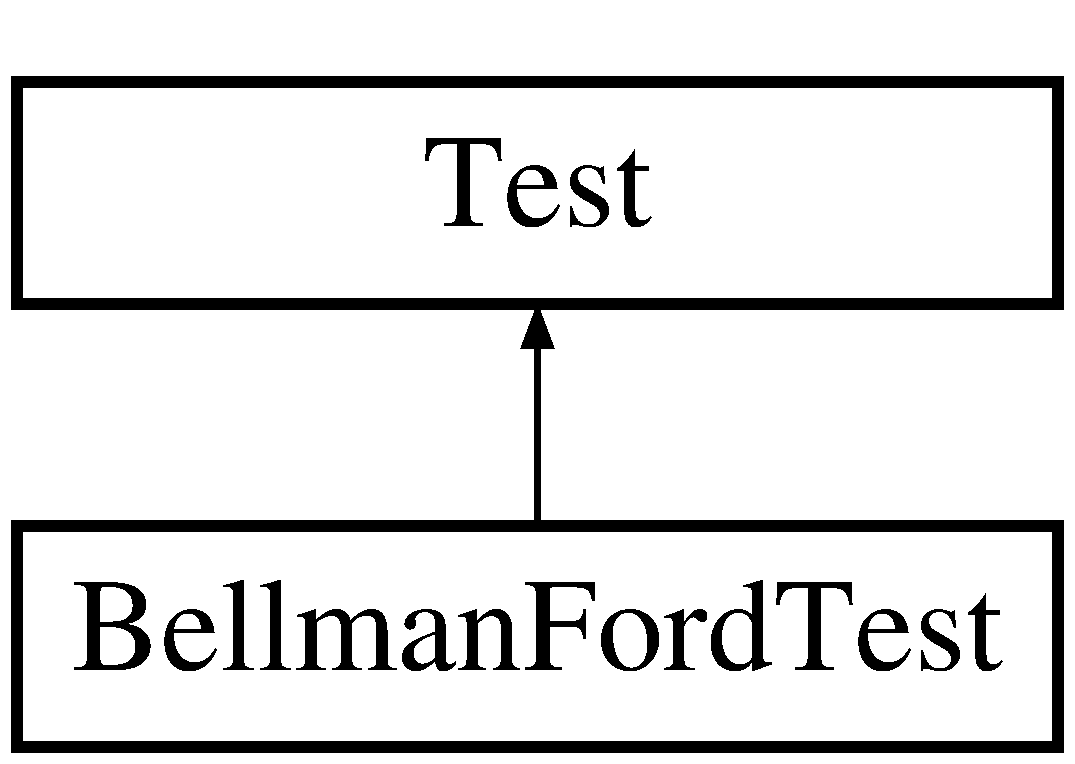
\includegraphics[height=2.000000cm]{class_bellman_ford_test}
\end{center}
\end{figure}
\subsection*{Public Types}
\begin{DoxyCompactItemize}
\item 
typedef \hyperlink{struct_introduction_to_algorithm_1_1_graph_algorithm_1_1_graph}{Graph}$<$ B\+\_\+\+N\+U\+M, \hyperlink{struct_introduction_to_algorithm_1_1_graph_algorithm_1_1_vertex_p}{Vertex\+P}$<$ int $>$ $>$ \hyperlink{class_bellman_ford_test_a81e8794fcae1d04ceb23de43c5944829}{Graph\+Type}
\item 
typedef \hyperlink{struct_introduction_to_algorithm_1_1_graph_algorithm_1_1_vertex_p}{Vertex\+P}$<$ int $>$ \hyperlink{class_bellman_ford_test_a823a571f7e631ee9e4f712440b35159d}{Vertex\+Type}
\end{DoxyCompactItemize}
\subsection*{Protected Member Functions}
\begin{DoxyCompactItemize}
\item 
void \hyperlink{class_bellman_ford_test_a8cb2e8d725e4c06914dafc73c73d94c6}{Set\+Up} ()
\item 
void \hyperlink{class_bellman_ford_test_a16ea847b45d890f27adf9381decdb5c8}{Tear\+Down} ()
\end{DoxyCompactItemize}
\subsection*{Protected Attributes}
\begin{DoxyCompactItemize}
\item 
std\+::shared\+\_\+ptr$<$ \hyperlink{class_bellman_ford_test_a81e8794fcae1d04ceb23de43c5944829}{Graph\+Type} $>$ \hyperlink{class_bellman_ford_test_a1e228fdc8f10f3932dfa93969b22740a}{\+\_\+1v\+\_\+graph}
\item 
std\+::shared\+\_\+ptr$<$ \hyperlink{class_bellman_ford_test_a81e8794fcae1d04ceb23de43c5944829}{Graph\+Type} $>$ \hyperlink{class_bellman_ford_test_a13720ba4e090b0accf73283c15a7f0ec}{\+\_\+1e\+\_\+graph}
\item 
std\+::shared\+\_\+ptr$<$ \hyperlink{class_bellman_ford_test_a81e8794fcae1d04ceb23de43c5944829}{Graph\+Type} $>$ \hyperlink{class_bellman_ford_test_a80eda504410ddbef790a30a0d4049185}{\+\_\+normal\+\_\+graph}
\item 
std\+::shared\+\_\+ptr$<$ \hyperlink{class_bellman_ford_test_a81e8794fcae1d04ceb23de43c5944829}{Graph\+Type} $>$ \hyperlink{class_bellman_ford_test_a179a0a6d2ae9d6a2404ef5e5f9a06869}{\+\_\+minus\+\_\+graph}
\end{DoxyCompactItemize}


\subsection{Detailed Description}
\hyperlink{class_bellman_ford_test}{Bellman\+Ford\+Test}\+:测试类,用于为测试提供基础数据 

{\ttfamily \hyperlink{class_bellman_ford_test}{Bellman\+Ford\+Test}}是 {\ttfamily \+::testing\+::\+Test} 的子类。它主要用于为每一个{\ttfamily T\+E\+S\+T\+\_\+\+F}准备测试环境 

Definition at line 40 of file bellmanford\+\_\+test.\+h.



\subsection{Member Typedef Documentation}
\hypertarget{class_bellman_ford_test_a81e8794fcae1d04ceb23de43c5944829}{}\index{Bellman\+Ford\+Test@{Bellman\+Ford\+Test}!Graph\+Type@{Graph\+Type}}
\index{Graph\+Type@{Graph\+Type}!Bellman\+Ford\+Test@{Bellman\+Ford\+Test}}
\subsubsection[{Graph\+Type}]{\setlength{\rightskip}{0pt plus 5cm}typedef {\bf Graph}$<$B\+\_\+\+N\+U\+M,{\bf Vertex\+P}$<$int$>$ $>$ {\bf Bellman\+Ford\+Test\+::\+Graph\+Type}}\label{class_bellman_ford_test_a81e8794fcae1d04ceb23de43c5944829}
模板实例化的图类型,该图的顶点类型为{\ttfamily Vertex\+P$<$int$>$} 

Definition at line 43 of file bellmanford\+\_\+test.\+h.

\hypertarget{class_bellman_ford_test_a823a571f7e631ee9e4f712440b35159d}{}\index{Bellman\+Ford\+Test@{Bellman\+Ford\+Test}!Vertex\+Type@{Vertex\+Type}}
\index{Vertex\+Type@{Vertex\+Type}!Bellman\+Ford\+Test@{Bellman\+Ford\+Test}}
\subsubsection[{Vertex\+Type}]{\setlength{\rightskip}{0pt plus 5cm}typedef {\bf Vertex\+P}$<$int$>$ {\bf Bellman\+Ford\+Test\+::\+Vertex\+Type}}\label{class_bellman_ford_test_a823a571f7e631ee9e4f712440b35159d}
图的顶点类型为{\ttfamily Vertex\+P$<$int$>$} 

Definition at line 44 of file bellmanford\+\_\+test.\+h.



\subsection{Member Function Documentation}
\hypertarget{class_bellman_ford_test_a8cb2e8d725e4c06914dafc73c73d94c6}{}\index{Bellman\+Ford\+Test@{Bellman\+Ford\+Test}!Set\+Up@{Set\+Up}}
\index{Set\+Up@{Set\+Up}!Bellman\+Ford\+Test@{Bellman\+Ford\+Test}}
\subsubsection[{Set\+Up()}]{\setlength{\rightskip}{0pt plus 5cm}void Bellman\+Ford\+Test\+::\+Set\+Up (
\begin{DoxyParamCaption}
{}
\end{DoxyParamCaption}
)\hspace{0.3cm}{\ttfamily [inline]}, {\ttfamily [protected]}}\label{class_bellman_ford_test_a8cb2e8d725e4c06914dafc73c73d94c6}


Definition at line 46 of file bellmanford\+\_\+test.\+h.

\hypertarget{class_bellman_ford_test_a16ea847b45d890f27adf9381decdb5c8}{}\index{Bellman\+Ford\+Test@{Bellman\+Ford\+Test}!Tear\+Down@{Tear\+Down}}
\index{Tear\+Down@{Tear\+Down}!Bellman\+Ford\+Test@{Bellman\+Ford\+Test}}
\subsubsection[{Tear\+Down()}]{\setlength{\rightskip}{0pt plus 5cm}void Bellman\+Ford\+Test\+::\+Tear\+Down (
\begin{DoxyParamCaption}
{}
\end{DoxyParamCaption}
)\hspace{0.3cm}{\ttfamily [inline]}, {\ttfamily [protected]}}\label{class_bellman_ford_test_a16ea847b45d890f27adf9381decdb5c8}


Definition at line 72 of file bellmanford\+\_\+test.\+h.



\subsection{Member Data Documentation}
\hypertarget{class_bellman_ford_test_a13720ba4e090b0accf73283c15a7f0ec}{}\index{Bellman\+Ford\+Test@{Bellman\+Ford\+Test}!\+\_\+1e\+\_\+graph@{\+\_\+1e\+\_\+graph}}
\index{\+\_\+1e\+\_\+graph@{\+\_\+1e\+\_\+graph}!Bellman\+Ford\+Test@{Bellman\+Ford\+Test}}
\subsubsection[{\+\_\+1e\+\_\+graph}]{\setlength{\rightskip}{0pt plus 5cm}std\+::shared\+\_\+ptr$<${\bf Graph\+Type}$>$ Bellman\+Ford\+Test\+::\+\_\+1e\+\_\+graph\hspace{0.3cm}{\ttfamily [protected]}}\label{class_bellman_ford_test_a13720ba4e090b0accf73283c15a7f0ec}
指向一个图,该图只有一条边 

Definition at line 75 of file bellmanford\+\_\+test.\+h.

\hypertarget{class_bellman_ford_test_a1e228fdc8f10f3932dfa93969b22740a}{}\index{Bellman\+Ford\+Test@{Bellman\+Ford\+Test}!\+\_\+1v\+\_\+graph@{\+\_\+1v\+\_\+graph}}
\index{\+\_\+1v\+\_\+graph@{\+\_\+1v\+\_\+graph}!Bellman\+Ford\+Test@{Bellman\+Ford\+Test}}
\subsubsection[{\+\_\+1v\+\_\+graph}]{\setlength{\rightskip}{0pt plus 5cm}std\+::shared\+\_\+ptr$<${\bf Graph\+Type}$>$ Bellman\+Ford\+Test\+::\+\_\+1v\+\_\+graph\hspace{0.3cm}{\ttfamily [protected]}}\label{class_bellman_ford_test_a1e228fdc8f10f3932dfa93969b22740a}
指向一个图,该图只有一个顶点 

Definition at line 74 of file bellmanford\+\_\+test.\+h.

\hypertarget{class_bellman_ford_test_a179a0a6d2ae9d6a2404ef5e5f9a06869}{}\index{Bellman\+Ford\+Test@{Bellman\+Ford\+Test}!\+\_\+minus\+\_\+graph@{\+\_\+minus\+\_\+graph}}
\index{\+\_\+minus\+\_\+graph@{\+\_\+minus\+\_\+graph}!Bellman\+Ford\+Test@{Bellman\+Ford\+Test}}
\subsubsection[{\+\_\+minus\+\_\+graph}]{\setlength{\rightskip}{0pt plus 5cm}std\+::shared\+\_\+ptr$<${\bf Graph\+Type}$>$ Bellman\+Ford\+Test\+::\+\_\+minus\+\_\+graph\hspace{0.3cm}{\ttfamily [protected]}}\label{class_bellman_ford_test_a179a0a6d2ae9d6a2404ef5e5f9a06869}
指向一个图,该图的边包含负权值回路 

Definition at line 77 of file bellmanford\+\_\+test.\+h.

\hypertarget{class_bellman_ford_test_a80eda504410ddbef790a30a0d4049185}{}\index{Bellman\+Ford\+Test@{Bellman\+Ford\+Test}!\+\_\+normal\+\_\+graph@{\+\_\+normal\+\_\+graph}}
\index{\+\_\+normal\+\_\+graph@{\+\_\+normal\+\_\+graph}!Bellman\+Ford\+Test@{Bellman\+Ford\+Test}}
\subsubsection[{\+\_\+normal\+\_\+graph}]{\setlength{\rightskip}{0pt plus 5cm}std\+::shared\+\_\+ptr$<${\bf Graph\+Type}$>$ Bellman\+Ford\+Test\+::\+\_\+normal\+\_\+graph\hspace{0.3cm}{\ttfamily [protected]}}\label{class_bellman_ford_test_a80eda504410ddbef790a30a0d4049185}
指向一个图,该图的边组成一条链条 

Definition at line 76 of file bellmanford\+\_\+test.\+h.



The documentation for this class was generated from the following file\+:\begin{DoxyCompactItemize}
\item 
src/graph\+\_\+algorithms/single\+\_\+source\+\_\+shortest\+\_\+path/bellman\+\_\+ford/\hyperlink{bellmanford__test_8h}{bellmanford\+\_\+test.\+h}\end{DoxyCompactItemize}

\hypertarget{struct_introduction_to_algorithm_1_1_graph_algorithm_1_1_b_f_s___vertex}{}\section{Introduction\+To\+Algorithm\+:\+:Graph\+Algorithm\+:\+:B\+F\+S\+\_\+\+Vertex$<$ K\+Type $>$ Struct Template Reference}
\label{struct_introduction_to_algorithm_1_1_graph_algorithm_1_1_b_f_s___vertex}\index{Introduction\+To\+Algorithm\+::\+Graph\+Algorithm\+::\+B\+F\+S\+\_\+\+Vertex$<$ K\+Type $>$@{Introduction\+To\+Algorithm\+::\+Graph\+Algorithm\+::\+B\+F\+S\+\_\+\+Vertex$<$ K\+Type $>$}}


B\+F\+S\+\_\+\+Vertex:用于广度优先搜索的顶点类型,算法导论22章22.2节  




{\ttfamily \#include $<$bfs\+\_\+vertex.\+h$>$}

Inheritance diagram for Introduction\+To\+Algorithm\+:\+:Graph\+Algorithm\+:\+:B\+F\+S\+\_\+\+Vertex$<$ K\+Type $>$\+:\begin{figure}[H]
\begin{center}
\leavevmode
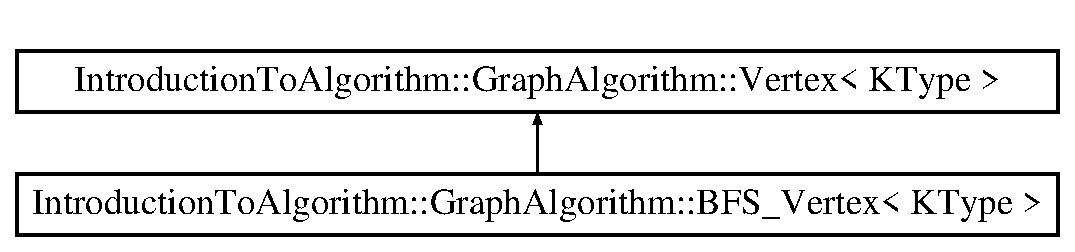
\includegraphics[height=2.000000cm]{struct_introduction_to_algorithm_1_1_graph_algorithm_1_1_b_f_s___vertex}
\end{center}
\end{figure}
\subsection*{Public Types}
\begin{DoxyCompactItemize}
\item 
enum \hyperlink{struct_introduction_to_algorithm_1_1_graph_algorithm_1_1_b_f_s___vertex_a3f00f12565def71750f1f163e0e52305}{C\+O\+L\+O\+R} \{ \hyperlink{struct_introduction_to_algorithm_1_1_graph_algorithm_1_1_b_f_s___vertex_a3f00f12565def71750f1f163e0e52305ab5bf627e448384cf3a4c35121ca6008d}{C\+O\+L\+O\+R\+::\+W\+H\+I\+T\+E}, 
\hyperlink{struct_introduction_to_algorithm_1_1_graph_algorithm_1_1_b_f_s___vertex_a3f00f12565def71750f1f163e0e52305a48bf014c704c9eaae100a98006a37bf7}{C\+O\+L\+O\+R\+::\+G\+R\+A\+Y}, 
\hyperlink{struct_introduction_to_algorithm_1_1_graph_algorithm_1_1_b_f_s___vertex_a3f00f12565def71750f1f163e0e52305a08d0012388564e95c3b4a7407cf04965}{C\+O\+L\+O\+R\+::\+B\+L\+A\+C\+K}
 \}
\item 
typedef int \hyperlink{struct_introduction_to_algorithm_1_1_graph_algorithm_1_1_b_f_s___vertex_a62cef758843cdaeefae2fc196f6bdb46}{V\+I\+D\+Type}
\item 
typedef K\+Type \hyperlink{struct_introduction_to_algorithm_1_1_graph_algorithm_1_1_b_f_s___vertex_a1e47ba34939458c68d7ccee8ebeccad2}{Key\+Type}
\end{DoxyCompactItemize}
\subsection*{Public Member Functions}
\begin{DoxyCompactItemize}
\item 
\hyperlink{struct_introduction_to_algorithm_1_1_graph_algorithm_1_1_b_f_s___vertex_ad9540a9d7487eea8ece6ac1b0bbfcc22}{B\+F\+S\+\_\+\+Vertex} ()
\begin{DoxyCompactList}\small\item\em 默认构造函数,将{\ttfamily color}设为白色 \end{DoxyCompactList}\item 
\hyperlink{struct_introduction_to_algorithm_1_1_graph_algorithm_1_1_b_f_s___vertex_abf41ef42dff5af509e9b42658882f604}{B\+F\+S\+\_\+\+Vertex} (const \hyperlink{struct_introduction_to_algorithm_1_1_graph_algorithm_1_1_b_f_s___vertex_a1e47ba34939458c68d7ccee8ebeccad2}{Key\+Type} \&k)
\begin{DoxyCompactList}\small\item\em 显式构造函数,指定{\ttfamily key} \end{DoxyCompactList}\item 
\hyperlink{struct_introduction_to_algorithm_1_1_graph_algorithm_1_1_b_f_s___vertex_a3765fd695d8452180bafbb42baec744f}{B\+F\+S\+\_\+\+Vertex} (const \hyperlink{struct_introduction_to_algorithm_1_1_graph_algorithm_1_1_b_f_s___vertex_a1e47ba34939458c68d7ccee8ebeccad2}{Key\+Type} \&k, \hyperlink{struct_introduction_to_algorithm_1_1_graph_algorithm_1_1_b_f_s___vertex_a62cef758843cdaeefae2fc196f6bdb46}{V\+I\+D\+Type} d)
\begin{DoxyCompactList}\small\item\em 显式构造函数,指定{\ttfamily key}和编号 \end{DoxyCompactList}\item 
void \hyperlink{struct_introduction_to_algorithm_1_1_graph_algorithm_1_1_b_f_s___vertex_a3f5b9ba686fae02e01cd899261fe6793}{set\+\_\+source} ()
\begin{DoxyCompactList}\small\item\em set\+\_\+source:设本顶点为源点 \end{DoxyCompactList}\item 
void \hyperlink{struct_introduction_to_algorithm_1_1_graph_algorithm_1_1_b_f_s___vertex_a7e523d76f261801c3622f00458333320}{set\+\_\+found} (std\+::shared\+\_\+ptr$<$ \hyperlink{struct_introduction_to_algorithm_1_1_graph_algorithm_1_1_b_f_s___vertex}{B\+F\+S\+\_\+\+Vertex} $>$ v\+\_\+parent)
\begin{DoxyCompactList}\small\item\em set\+\_\+found:发现本顶点 \end{DoxyCompactList}\item 
std\+::string \hyperlink{struct_introduction_to_algorithm_1_1_graph_algorithm_1_1_b_f_s___vertex_a73aa1fb33a2616818b709d04e79a007e}{to\+\_\+string} ()
\begin{DoxyCompactList}\small\item\em to\+\_\+string:返回顶点的字符串描述 \end{DoxyCompactList}\end{DoxyCompactItemize}
\subsection*{Public Attributes}
\begin{DoxyCompactItemize}
\item 
\hyperlink{struct_introduction_to_algorithm_1_1_graph_algorithm_1_1_b_f_s___vertex_a3f00f12565def71750f1f163e0e52305}{C\+O\+L\+O\+R} \hyperlink{struct_introduction_to_algorithm_1_1_graph_algorithm_1_1_b_f_s___vertex_a7ab527ab8514bcb65e56edbe62b28fbb}{color}
\item 
std\+::shared\+\_\+ptr$<$ \hyperlink{struct_introduction_to_algorithm_1_1_graph_algorithm_1_1_b_f_s___vertex}{B\+F\+S\+\_\+\+Vertex} $>$ \hyperlink{struct_introduction_to_algorithm_1_1_graph_algorithm_1_1_b_f_s___vertex_a11202710469656d7fb04635430355c41}{parent}
\end{DoxyCompactItemize}


\subsection{Detailed Description}
\subsubsection*{template$<$typename K\+Type$>$struct Introduction\+To\+Algorithm\+::\+Graph\+Algorithm\+::\+B\+F\+S\+\_\+\+Vertex$<$ K\+Type $>$}

B\+F\+S\+\_\+\+Vertex:用于广度优先搜索的顶点类型,算法导论22章22.2节 

广度优先搜索的顶点类型继承自{\ttfamily \hyperlink{struct_introduction_to_algorithm_1_1_graph_algorithm_1_1_vertex}{Vertex}}模板类型,它比{\ttfamily \hyperlink{struct_introduction_to_algorithm_1_1_graph_algorithm_1_1_vertex}{Vertex}}多了两个数据成员:


\begin{DoxyItemize}
\item {\ttfamily color}:顶点的颜色。顶点可以有三种颜色,分别为{\ttfamily \hyperlink{struct_introduction_to_algorithm_1_1_graph_algorithm_1_1_b_f_s___vertex_a3f00f12565def71750f1f163e0e52305a08d0012388564e95c3b4a7407cf04965}{B\+F\+S\+\_\+\+Vertex\+::\+C\+O\+L\+O\+R\+::\+B\+L\+A\+C\+K}}、{\ttfamily \hyperlink{struct_introduction_to_algorithm_1_1_graph_algorithm_1_1_b_f_s___vertex_a3f00f12565def71750f1f163e0e52305ab5bf627e448384cf3a4c35121ca6008d}{B\+F\+S\+\_\+\+Vertex\+::\+C\+O\+L\+O\+R\+::\+W\+H\+I\+T\+E}}、{\ttfamily \hyperlink{struct_introduction_to_algorithm_1_1_graph_algorithm_1_1_b_f_s___vertex_a3f00f12565def71750f1f163e0e52305a48bf014c704c9eaae100a98006a37bf7}{B\+F\+S\+\_\+\+Vertex\+::\+C\+O\+L\+O\+R\+::\+G\+R\+A\+Y}}
\item {\ttfamily parent}\+: 指向父顶点的强引用
\end{DoxyItemize}

广度优先搜索的顶点类型还支持以下两个操作:


\begin{DoxyItemize}
\item {\ttfamily \hyperlink{struct_introduction_to_algorithm_1_1_graph_algorithm_1_1_b_f_s___vertex_a3f5b9ba686fae02e01cd899261fe6793}{set\+\_\+source()}}:将本顶点设为源点
\item {\ttfamily set\+\_\+found(v\+\_\+parent)}:发现本顶点 
\end{DoxyItemize}

Definition at line 42 of file bfs\+\_\+vertex.\+h.



\subsection{Member Typedef Documentation}
\hypertarget{struct_introduction_to_algorithm_1_1_graph_algorithm_1_1_b_f_s___vertex_a1e47ba34939458c68d7ccee8ebeccad2}{}\index{Introduction\+To\+Algorithm\+::\+Graph\+Algorithm\+::\+B\+F\+S\+\_\+\+Vertex@{Introduction\+To\+Algorithm\+::\+Graph\+Algorithm\+::\+B\+F\+S\+\_\+\+Vertex}!Key\+Type@{Key\+Type}}
\index{Key\+Type@{Key\+Type}!Introduction\+To\+Algorithm\+::\+Graph\+Algorithm\+::\+B\+F\+S\+\_\+\+Vertex@{Introduction\+To\+Algorithm\+::\+Graph\+Algorithm\+::\+B\+F\+S\+\_\+\+Vertex}}
\subsubsection[{Key\+Type}]{\setlength{\rightskip}{0pt plus 5cm}template$<$typename K\+Type $>$ typedef K\+Type {\bf Introduction\+To\+Algorithm\+::\+Graph\+Algorithm\+::\+B\+F\+S\+\_\+\+Vertex}$<$ K\+Type $>$\+::{\bf Key\+Type}}\label{struct_introduction_to_algorithm_1_1_graph_algorithm_1_1_b_f_s___vertex_a1e47ba34939458c68d7ccee8ebeccad2}
顶点存储数据的类型 

Definition at line 46 of file bfs\+\_\+vertex.\+h.

\hypertarget{struct_introduction_to_algorithm_1_1_graph_algorithm_1_1_b_f_s___vertex_a62cef758843cdaeefae2fc196f6bdb46}{}\index{Introduction\+To\+Algorithm\+::\+Graph\+Algorithm\+::\+B\+F\+S\+\_\+\+Vertex@{Introduction\+To\+Algorithm\+::\+Graph\+Algorithm\+::\+B\+F\+S\+\_\+\+Vertex}!V\+I\+D\+Type@{V\+I\+D\+Type}}
\index{V\+I\+D\+Type@{V\+I\+D\+Type}!Introduction\+To\+Algorithm\+::\+Graph\+Algorithm\+::\+B\+F\+S\+\_\+\+Vertex@{Introduction\+To\+Algorithm\+::\+Graph\+Algorithm\+::\+B\+F\+S\+\_\+\+Vertex}}
\subsubsection[{V\+I\+D\+Type}]{\setlength{\rightskip}{0pt plus 5cm}template$<$typename K\+Type $>$ typedef int {\bf Introduction\+To\+Algorithm\+::\+Graph\+Algorithm\+::\+B\+F\+S\+\_\+\+Vertex}$<$ K\+Type $>$\+::{\bf V\+I\+D\+Type}}\label{struct_introduction_to_algorithm_1_1_graph_algorithm_1_1_b_f_s___vertex_a62cef758843cdaeefae2fc196f6bdb46}
顶点编号的数据类型 

Definition at line 45 of file bfs\+\_\+vertex.\+h.



\subsection{Member Enumeration Documentation}
\hypertarget{struct_introduction_to_algorithm_1_1_graph_algorithm_1_1_b_f_s___vertex_a3f00f12565def71750f1f163e0e52305}{}\index{Introduction\+To\+Algorithm\+::\+Graph\+Algorithm\+::\+B\+F\+S\+\_\+\+Vertex@{Introduction\+To\+Algorithm\+::\+Graph\+Algorithm\+::\+B\+F\+S\+\_\+\+Vertex}!C\+O\+L\+O\+R@{C\+O\+L\+O\+R}}
\index{C\+O\+L\+O\+R@{C\+O\+L\+O\+R}!Introduction\+To\+Algorithm\+::\+Graph\+Algorithm\+::\+B\+F\+S\+\_\+\+Vertex@{Introduction\+To\+Algorithm\+::\+Graph\+Algorithm\+::\+B\+F\+S\+\_\+\+Vertex}}
\subsubsection[{C\+O\+L\+O\+R}]{\setlength{\rightskip}{0pt plus 5cm}template$<$typename K\+Type $>$ enum {\bf Introduction\+To\+Algorithm\+::\+Graph\+Algorithm\+::\+B\+F\+S\+\_\+\+Vertex\+::\+C\+O\+L\+O\+R}\hspace{0.3cm}{\ttfamily [strong]}}\label{struct_introduction_to_algorithm_1_1_graph_algorithm_1_1_b_f_s___vertex_a3f00f12565def71750f1f163e0e52305}
\begin{Desc}
\item[Enumerator]\par
\begin{description}
\index{W\+H\+I\+T\+E@{W\+H\+I\+T\+E}!Introduction\+To\+Algorithm\+::\+Graph\+Algorithm\+::\+B\+F\+S\+\_\+\+Vertex@{Introduction\+To\+Algorithm\+::\+Graph\+Algorithm\+::\+B\+F\+S\+\_\+\+Vertex}}\index{Introduction\+To\+Algorithm\+::\+Graph\+Algorithm\+::\+B\+F\+S\+\_\+\+Vertex@{Introduction\+To\+Algorithm\+::\+Graph\+Algorithm\+::\+B\+F\+S\+\_\+\+Vertex}!W\+H\+I\+T\+E@{W\+H\+I\+T\+E}}\item[{\em 
\hypertarget{struct_introduction_to_algorithm_1_1_graph_algorithm_1_1_b_f_s___vertex_a3f00f12565def71750f1f163e0e52305ab5bf627e448384cf3a4c35121ca6008d}{}W\+H\+I\+T\+E\label{struct_introduction_to_algorithm_1_1_graph_algorithm_1_1_b_f_s___vertex_a3f00f12565def71750f1f163e0e52305ab5bf627e448384cf3a4c35121ca6008d}
}]\index{G\+R\+A\+Y@{G\+R\+A\+Y}!Introduction\+To\+Algorithm\+::\+Graph\+Algorithm\+::\+B\+F\+S\+\_\+\+Vertex@{Introduction\+To\+Algorithm\+::\+Graph\+Algorithm\+::\+B\+F\+S\+\_\+\+Vertex}}\index{Introduction\+To\+Algorithm\+::\+Graph\+Algorithm\+::\+B\+F\+S\+\_\+\+Vertex@{Introduction\+To\+Algorithm\+::\+Graph\+Algorithm\+::\+B\+F\+S\+\_\+\+Vertex}!G\+R\+A\+Y@{G\+R\+A\+Y}}\item[{\em 
\hypertarget{struct_introduction_to_algorithm_1_1_graph_algorithm_1_1_b_f_s___vertex_a3f00f12565def71750f1f163e0e52305a48bf014c704c9eaae100a98006a37bf7}{}G\+R\+A\+Y\label{struct_introduction_to_algorithm_1_1_graph_algorithm_1_1_b_f_s___vertex_a3f00f12565def71750f1f163e0e52305a48bf014c704c9eaae100a98006a37bf7}
}]\index{B\+L\+A\+C\+K@{B\+L\+A\+C\+K}!Introduction\+To\+Algorithm\+::\+Graph\+Algorithm\+::\+B\+F\+S\+\_\+\+Vertex@{Introduction\+To\+Algorithm\+::\+Graph\+Algorithm\+::\+B\+F\+S\+\_\+\+Vertex}}\index{Introduction\+To\+Algorithm\+::\+Graph\+Algorithm\+::\+B\+F\+S\+\_\+\+Vertex@{Introduction\+To\+Algorithm\+::\+Graph\+Algorithm\+::\+B\+F\+S\+\_\+\+Vertex}!B\+L\+A\+C\+K@{B\+L\+A\+C\+K}}\item[{\em 
\hypertarget{struct_introduction_to_algorithm_1_1_graph_algorithm_1_1_b_f_s___vertex_a3f00f12565def71750f1f163e0e52305a08d0012388564e95c3b4a7407cf04965}{}B\+L\+A\+C\+K\label{struct_introduction_to_algorithm_1_1_graph_algorithm_1_1_b_f_s___vertex_a3f00f12565def71750f1f163e0e52305a08d0012388564e95c3b4a7407cf04965}
}]\end{description}
\end{Desc}


Definition at line 47 of file bfs\+\_\+vertex.\+h.



\subsection{Constructor \& Destructor Documentation}
\hypertarget{struct_introduction_to_algorithm_1_1_graph_algorithm_1_1_b_f_s___vertex_ad9540a9d7487eea8ece6ac1b0bbfcc22}{}\index{Introduction\+To\+Algorithm\+::\+Graph\+Algorithm\+::\+B\+F\+S\+\_\+\+Vertex@{Introduction\+To\+Algorithm\+::\+Graph\+Algorithm\+::\+B\+F\+S\+\_\+\+Vertex}!B\+F\+S\+\_\+\+Vertex@{B\+F\+S\+\_\+\+Vertex}}
\index{B\+F\+S\+\_\+\+Vertex@{B\+F\+S\+\_\+\+Vertex}!Introduction\+To\+Algorithm\+::\+Graph\+Algorithm\+::\+B\+F\+S\+\_\+\+Vertex@{Introduction\+To\+Algorithm\+::\+Graph\+Algorithm\+::\+B\+F\+S\+\_\+\+Vertex}}
\subsubsection[{B\+F\+S\+\_\+\+Vertex()}]{\setlength{\rightskip}{0pt plus 5cm}template$<$typename K\+Type $>$ {\bf Introduction\+To\+Algorithm\+::\+Graph\+Algorithm\+::\+B\+F\+S\+\_\+\+Vertex}$<$ K\+Type $>$\+::{\bf B\+F\+S\+\_\+\+Vertex} (
\begin{DoxyParamCaption}
{}
\end{DoxyParamCaption}
)\hspace{0.3cm}{\ttfamily [inline]}}\label{struct_introduction_to_algorithm_1_1_graph_algorithm_1_1_b_f_s___vertex_ad9540a9d7487eea8ece6ac1b0bbfcc22}


默认构造函数,将{\ttfamily color}设为白色 



Definition at line 51 of file bfs\+\_\+vertex.\+h.

\hypertarget{struct_introduction_to_algorithm_1_1_graph_algorithm_1_1_b_f_s___vertex_abf41ef42dff5af509e9b42658882f604}{}\index{Introduction\+To\+Algorithm\+::\+Graph\+Algorithm\+::\+B\+F\+S\+\_\+\+Vertex@{Introduction\+To\+Algorithm\+::\+Graph\+Algorithm\+::\+B\+F\+S\+\_\+\+Vertex}!B\+F\+S\+\_\+\+Vertex@{B\+F\+S\+\_\+\+Vertex}}
\index{B\+F\+S\+\_\+\+Vertex@{B\+F\+S\+\_\+\+Vertex}!Introduction\+To\+Algorithm\+::\+Graph\+Algorithm\+::\+B\+F\+S\+\_\+\+Vertex@{Introduction\+To\+Algorithm\+::\+Graph\+Algorithm\+::\+B\+F\+S\+\_\+\+Vertex}}
\subsubsection[{B\+F\+S\+\_\+\+Vertex(const Key\+Type \&k)}]{\setlength{\rightskip}{0pt plus 5cm}template$<$typename K\+Type $>$ {\bf Introduction\+To\+Algorithm\+::\+Graph\+Algorithm\+::\+B\+F\+S\+\_\+\+Vertex}$<$ K\+Type $>$\+::{\bf B\+F\+S\+\_\+\+Vertex} (
\begin{DoxyParamCaption}
\item[{const {\bf Key\+Type} \&}]{k}
\end{DoxyParamCaption}
)\hspace{0.3cm}{\ttfamily [inline]}, {\ttfamily [explicit]}}\label{struct_introduction_to_algorithm_1_1_graph_algorithm_1_1_b_f_s___vertex_abf41ef42dff5af509e9b42658882f604}


显式构造函数,指定{\ttfamily key} 


\begin{DoxyParams}{Parameters}
{\em k\+:顶点存放的数据} & 顶点的颜色默认设为白色 \\
\hline
\end{DoxyParams}


Definition at line 58 of file bfs\+\_\+vertex.\+h.

\hypertarget{struct_introduction_to_algorithm_1_1_graph_algorithm_1_1_b_f_s___vertex_a3765fd695d8452180bafbb42baec744f}{}\index{Introduction\+To\+Algorithm\+::\+Graph\+Algorithm\+::\+B\+F\+S\+\_\+\+Vertex@{Introduction\+To\+Algorithm\+::\+Graph\+Algorithm\+::\+B\+F\+S\+\_\+\+Vertex}!B\+F\+S\+\_\+\+Vertex@{B\+F\+S\+\_\+\+Vertex}}
\index{B\+F\+S\+\_\+\+Vertex@{B\+F\+S\+\_\+\+Vertex}!Introduction\+To\+Algorithm\+::\+Graph\+Algorithm\+::\+B\+F\+S\+\_\+\+Vertex@{Introduction\+To\+Algorithm\+::\+Graph\+Algorithm\+::\+B\+F\+S\+\_\+\+Vertex}}
\subsubsection[{B\+F\+S\+\_\+\+Vertex(const Key\+Type \&k, V\+I\+D\+Type d)}]{\setlength{\rightskip}{0pt plus 5cm}template$<$typename K\+Type $>$ {\bf Introduction\+To\+Algorithm\+::\+Graph\+Algorithm\+::\+B\+F\+S\+\_\+\+Vertex}$<$ K\+Type $>$\+::{\bf B\+F\+S\+\_\+\+Vertex} (
\begin{DoxyParamCaption}
\item[{const {\bf Key\+Type} \&}]{k, }
\item[{{\bf V\+I\+D\+Type}}]{d}
\end{DoxyParamCaption}
)\hspace{0.3cm}{\ttfamily [inline]}}\label{struct_introduction_to_algorithm_1_1_graph_algorithm_1_1_b_f_s___vertex_a3765fd695d8452180bafbb42baec744f}


显式构造函数,指定{\ttfamily key}和编号 


\begin{DoxyParams}{Parameters}
{\em k\+:顶点存放的数据} & \\
\hline
{\em d\+:顶点的编号} & 顶点的颜色默认设为白色 \\
\hline
\end{DoxyParams}


Definition at line 66 of file bfs\+\_\+vertex.\+h.



\subsection{Member Function Documentation}
\hypertarget{struct_introduction_to_algorithm_1_1_graph_algorithm_1_1_b_f_s___vertex_a7e523d76f261801c3622f00458333320}{}\index{Introduction\+To\+Algorithm\+::\+Graph\+Algorithm\+::\+B\+F\+S\+\_\+\+Vertex@{Introduction\+To\+Algorithm\+::\+Graph\+Algorithm\+::\+B\+F\+S\+\_\+\+Vertex}!set\+\_\+found@{set\+\_\+found}}
\index{set\+\_\+found@{set\+\_\+found}!Introduction\+To\+Algorithm\+::\+Graph\+Algorithm\+::\+B\+F\+S\+\_\+\+Vertex@{Introduction\+To\+Algorithm\+::\+Graph\+Algorithm\+::\+B\+F\+S\+\_\+\+Vertex}}
\subsubsection[{set\+\_\+found(std\+::shared\+\_\+ptr$<$ B\+F\+S\+\_\+\+Vertex $>$ v\+\_\+parent)}]{\setlength{\rightskip}{0pt plus 5cm}template$<$typename K\+Type $>$ void {\bf Introduction\+To\+Algorithm\+::\+Graph\+Algorithm\+::\+B\+F\+S\+\_\+\+Vertex}$<$ K\+Type $>$\+::set\+\_\+found (
\begin{DoxyParamCaption}
\item[{std\+::shared\+\_\+ptr$<$ {\bf B\+F\+S\+\_\+\+Vertex}$<$ K\+Type $>$ $>$}]{v\+\_\+parent}
\end{DoxyParamCaption}
)\hspace{0.3cm}{\ttfamily [inline]}}\label{struct_introduction_to_algorithm_1_1_graph_algorithm_1_1_b_f_s___vertex_a7e523d76f261801c3622f00458333320}


set\+\_\+found:发现本顶点 


\begin{DoxyParams}{Parameters}
{\em v\+\_\+parent\+:父顶点的强引用} & 发现本顶点要执行两个操作:\\
\hline
\end{DoxyParams}

\begin{DoxyItemize}
\item 将本顶点的颜色设为灰色
\item 将本顶点的{\ttfamily parent}设为{\ttfamily v\+\_\+parent}
\end{DoxyItemize}

这里要求{\ttfamily v\+\_\+parent}非空。若{\ttfamily v\+\_\+parent}为空则抛出异常 

Definition at line 94 of file bfs\+\_\+vertex.\+h.

\hypertarget{struct_introduction_to_algorithm_1_1_graph_algorithm_1_1_b_f_s___vertex_a3f5b9ba686fae02e01cd899261fe6793}{}\index{Introduction\+To\+Algorithm\+::\+Graph\+Algorithm\+::\+B\+F\+S\+\_\+\+Vertex@{Introduction\+To\+Algorithm\+::\+Graph\+Algorithm\+::\+B\+F\+S\+\_\+\+Vertex}!set\+\_\+source@{set\+\_\+source}}
\index{set\+\_\+source@{set\+\_\+source}!Introduction\+To\+Algorithm\+::\+Graph\+Algorithm\+::\+B\+F\+S\+\_\+\+Vertex@{Introduction\+To\+Algorithm\+::\+Graph\+Algorithm\+::\+B\+F\+S\+\_\+\+Vertex}}
\subsubsection[{set\+\_\+source()}]{\setlength{\rightskip}{0pt plus 5cm}template$<$typename K\+Type $>$ void {\bf Introduction\+To\+Algorithm\+::\+Graph\+Algorithm\+::\+B\+F\+S\+\_\+\+Vertex}$<$ K\+Type $>$\+::set\+\_\+source (
\begin{DoxyParamCaption}
{}
\end{DoxyParamCaption}
)\hspace{0.3cm}{\ttfamily [inline]}}\label{struct_introduction_to_algorithm_1_1_graph_algorithm_1_1_b_f_s___vertex_a3f5b9ba686fae02e01cd899261fe6793}


set\+\_\+source:设本顶点为源点 

将本顶点设为源点要执行两个操作:


\begin{DoxyItemize}
\item 将本顶点的颜色设为灰色
\item 将本顶点的{\ttfamily parent}设为空 
\end{DoxyItemize}

Definition at line 76 of file bfs\+\_\+vertex.\+h.

\hypertarget{struct_introduction_to_algorithm_1_1_graph_algorithm_1_1_b_f_s___vertex_a73aa1fb33a2616818b709d04e79a007e}{}\index{Introduction\+To\+Algorithm\+::\+Graph\+Algorithm\+::\+B\+F\+S\+\_\+\+Vertex@{Introduction\+To\+Algorithm\+::\+Graph\+Algorithm\+::\+B\+F\+S\+\_\+\+Vertex}!to\+\_\+string@{to\+\_\+string}}
\index{to\+\_\+string@{to\+\_\+string}!Introduction\+To\+Algorithm\+::\+Graph\+Algorithm\+::\+B\+F\+S\+\_\+\+Vertex@{Introduction\+To\+Algorithm\+::\+Graph\+Algorithm\+::\+B\+F\+S\+\_\+\+Vertex}}
\subsubsection[{to\+\_\+string()}]{\setlength{\rightskip}{0pt plus 5cm}template$<$typename K\+Type $>$ std\+::string {\bf Introduction\+To\+Algorithm\+::\+Graph\+Algorithm\+::\+B\+F\+S\+\_\+\+Vertex}$<$ K\+Type $>$\+::to\+\_\+string (
\begin{DoxyParamCaption}
{}
\end{DoxyParamCaption}
)\hspace{0.3cm}{\ttfamily [inline]}}\label{struct_introduction_to_algorithm_1_1_graph_algorithm_1_1_b_f_s___vertex_a73aa1fb33a2616818b709d04e79a007e}


to\+\_\+string:返回顶点的字符串描述 

\begin{DoxyReturn}{Returns}
\+:顶点的字符串描述
\end{DoxyReturn}
再{\ttfamily \hyperlink{struct_introduction_to_algorithm_1_1_graph_algorithm_1_1_vertex}{Vertex}}基类的基础上输出{\ttfamily color}以及{\ttfamily parent}信息。 

Definition at line 110 of file bfs\+\_\+vertex.\+h.



\subsection{Member Data Documentation}
\hypertarget{struct_introduction_to_algorithm_1_1_graph_algorithm_1_1_b_f_s___vertex_a7ab527ab8514bcb65e56edbe62b28fbb}{}\index{Introduction\+To\+Algorithm\+::\+Graph\+Algorithm\+::\+B\+F\+S\+\_\+\+Vertex@{Introduction\+To\+Algorithm\+::\+Graph\+Algorithm\+::\+B\+F\+S\+\_\+\+Vertex}!color@{color}}
\index{color@{color}!Introduction\+To\+Algorithm\+::\+Graph\+Algorithm\+::\+B\+F\+S\+\_\+\+Vertex@{Introduction\+To\+Algorithm\+::\+Graph\+Algorithm\+::\+B\+F\+S\+\_\+\+Vertex}}
\subsubsection[{color}]{\setlength{\rightskip}{0pt plus 5cm}template$<$typename K\+Type $>$ {\bf C\+O\+L\+O\+R} {\bf Introduction\+To\+Algorithm\+::\+Graph\+Algorithm\+::\+B\+F\+S\+\_\+\+Vertex}$<$ K\+Type $>$\+::color}\label{struct_introduction_to_algorithm_1_1_graph_algorithm_1_1_b_f_s___vertex_a7ab527ab8514bcb65e56edbe62b28fbb}
顶点颜色 

Definition at line 133 of file bfs\+\_\+vertex.\+h.

\hypertarget{struct_introduction_to_algorithm_1_1_graph_algorithm_1_1_b_f_s___vertex_a11202710469656d7fb04635430355c41}{}\index{Introduction\+To\+Algorithm\+::\+Graph\+Algorithm\+::\+B\+F\+S\+\_\+\+Vertex@{Introduction\+To\+Algorithm\+::\+Graph\+Algorithm\+::\+B\+F\+S\+\_\+\+Vertex}!parent@{parent}}
\index{parent@{parent}!Introduction\+To\+Algorithm\+::\+Graph\+Algorithm\+::\+B\+F\+S\+\_\+\+Vertex@{Introduction\+To\+Algorithm\+::\+Graph\+Algorithm\+::\+B\+F\+S\+\_\+\+Vertex}}
\subsubsection[{parent}]{\setlength{\rightskip}{0pt plus 5cm}template$<$typename K\+Type $>$ std\+::shared\+\_\+ptr$<${\bf B\+F\+S\+\_\+\+Vertex}$>$ {\bf Introduction\+To\+Algorithm\+::\+Graph\+Algorithm\+::\+B\+F\+S\+\_\+\+Vertex}$<$ K\+Type $>$\+::parent}\label{struct_introduction_to_algorithm_1_1_graph_algorithm_1_1_b_f_s___vertex_a11202710469656d7fb04635430355c41}
顶点父顶点的强引用 

Definition at line 134 of file bfs\+\_\+vertex.\+h.



The documentation for this struct was generated from the following file\+:\begin{DoxyCompactItemize}
\item 
src/graph\+\_\+algorithms/basic\+\_\+graph/graph\+\_\+representation/graph\+\_\+vertex/\hyperlink{bfs__vertex_8h}{bfs\+\_\+vertex.\+h}\end{DoxyCompactItemize}

\hypertarget{class_b_f_s_test}{}\section{B\+F\+S\+Test Class Reference}
\label{class_b_f_s_test}\index{B\+F\+S\+Test@{B\+F\+S\+Test}}


\hyperlink{class_b_f_s_test}{B\+F\+S\+Test}\+:测试类,用于为测试提供基础数据  




{\ttfamily \#include $<$bfs\+\_\+test.\+h$>$}

Inheritance diagram for B\+F\+S\+Test\+:\begin{figure}[H]
\begin{center}
\leavevmode
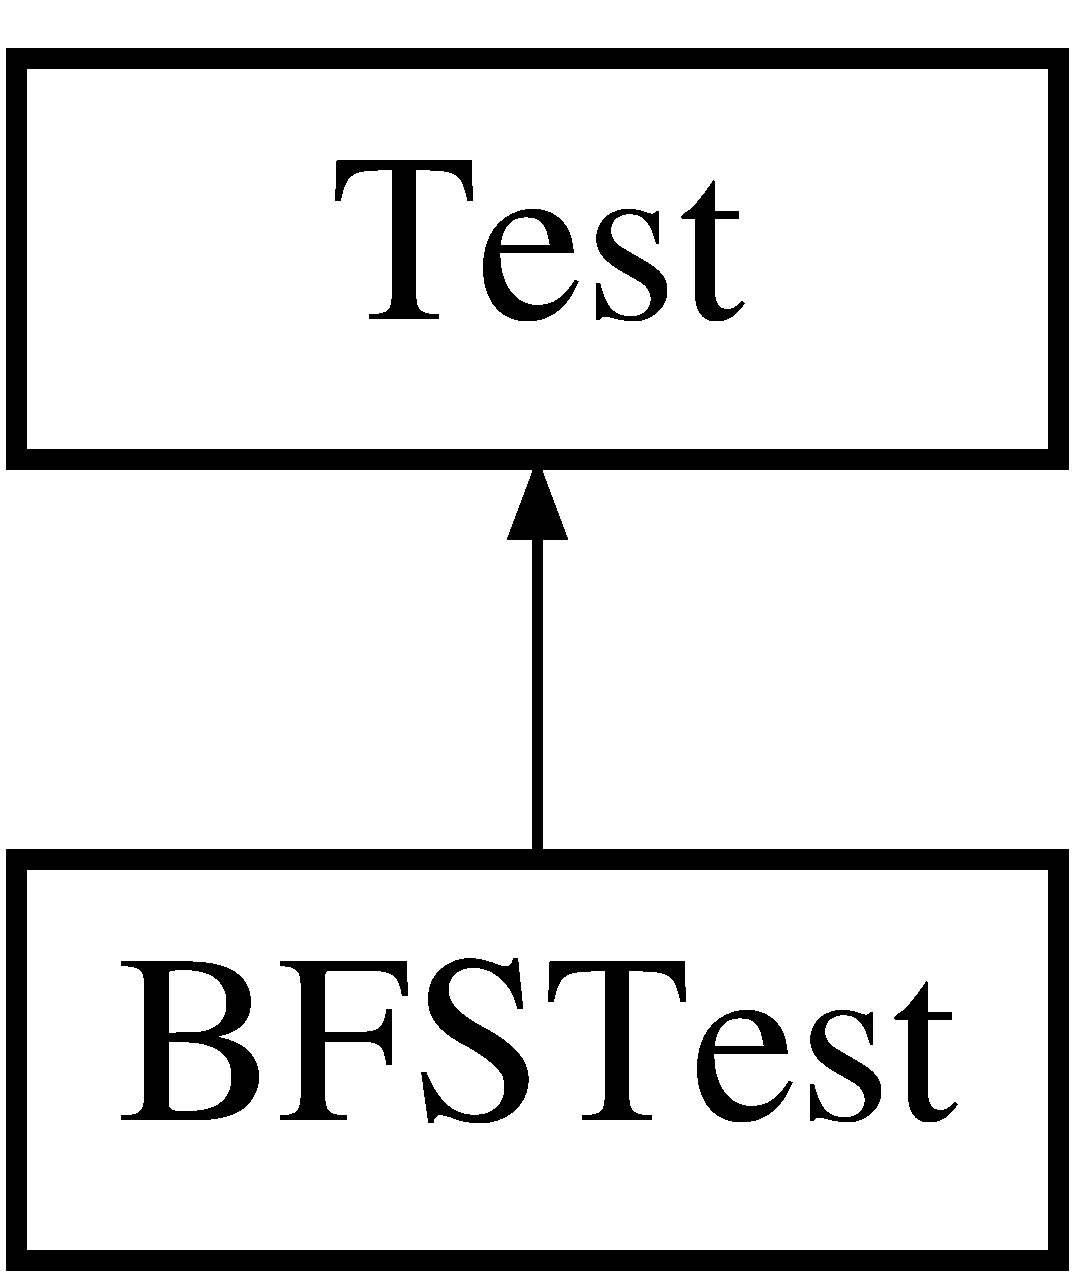
\includegraphics[height=2.000000cm]{class_b_f_s_test}
\end{center}
\end{figure}
\subsection*{Public Types}
\begin{DoxyCompactItemize}
\item 
typedef \hyperlink{struct_introduction_to_algorithm_1_1_graph_algorithm_1_1_graph}{Graph}$<$ B\+F\+S\+\_\+\+N, \hyperlink{struct_introduction_to_algorithm_1_1_graph_algorithm_1_1_b_f_s___vertex}{B\+F\+S\+\_\+\+Vertex}$<$ int $>$ $>$ \hyperlink{class_b_f_s_test_ad38ca5029d5674d467dc71d13f5e5c7c}{G\+Type}
\item 
typedef std\+::function$<$ void(\hyperlink{struct_introduction_to_algorithm_1_1_graph_algorithm_1_1_b_f_s___vertex}{B\+F\+S\+\_\+\+Vertex}$<$ int $>$\+::V\+I\+D\+Type v\+\_\+id)$>$ \hyperlink{class_b_f_s_test_a4012e860a3e78030ef0f4f544a834177}{Action\+Type}
\end{DoxyCompactItemize}
\subsection*{Protected Member Functions}
\begin{DoxyCompactItemize}
\item 
void \hyperlink{class_b_f_s_test_a295164608e7887ea16383eb80e0d2a45}{Set\+Up} ()
\item 
void \hyperlink{class_b_f_s_test_ac160dd8773850140c50cde59c8498764}{Tear\+Down} ()
\end{DoxyCompactItemize}
\subsection*{Protected Attributes}
\begin{DoxyCompactItemize}
\item 
std\+::shared\+\_\+ptr$<$ \hyperlink{class_b_f_s_test_ad38ca5029d5674d467dc71d13f5e5c7c}{G\+Type} $>$ \hyperlink{class_b_f_s_test_a0d7cdb7946902c8d93945a35a222b9d7}{\+\_\+1v\+\_\+graph}
\item 
std\+::shared\+\_\+ptr$<$ \hyperlink{class_b_f_s_test_ad38ca5029d5674d467dc71d13f5e5c7c}{G\+Type} $>$ \hyperlink{class_b_f_s_test_a0158014634e67e6bee3f8f6b1e622ced}{\+\_\+1e\+\_\+graph}
\item 
std\+::shared\+\_\+ptr$<$ \hyperlink{class_b_f_s_test_ad38ca5029d5674d467dc71d13f5e5c7c}{G\+Type} $>$ \hyperlink{class_b_f_s_test_aacf800be44976478c190b2acd338377f}{\+\_\+list\+\_\+graph}
\end{DoxyCompactItemize}


\subsection{Detailed Description}
\hyperlink{class_b_f_s_test}{B\+F\+S\+Test}\+:测试类,用于为测试提供基础数据 

{\ttfamily \hyperlink{class_b_f_s_test}{B\+F\+S\+Test}}是 {\ttfamily \+::testing\+::\+Test} 的子类。它主要用于为每一个{\ttfamily T\+E\+S\+T\+\_\+\+F}准备测试环境 

Definition at line 41 of file bfs\+\_\+test.\+h.



\subsection{Member Typedef Documentation}
\hypertarget{class_b_f_s_test_a4012e860a3e78030ef0f4f544a834177}{}\index{B\+F\+S\+Test@{B\+F\+S\+Test}!Action\+Type@{Action\+Type}}
\index{Action\+Type@{Action\+Type}!B\+F\+S\+Test@{B\+F\+S\+Test}}
\subsubsection[{Action\+Type}]{\setlength{\rightskip}{0pt plus 5cm}typedef std\+::function$<$void({\bf B\+F\+S\+\_\+\+Vertex}$<$int$>$\+::V\+I\+D\+Type v\+\_\+id)$>$ {\bf B\+F\+S\+Test\+::\+Action\+Type}}\label{class_b_f_s_test_a4012e860a3e78030ef0f4f544a834177}
模板实例化的\+Action类型 

Definition at line 45 of file bfs\+\_\+test.\+h.

\hypertarget{class_b_f_s_test_ad38ca5029d5674d467dc71d13f5e5c7c}{}\index{B\+F\+S\+Test@{B\+F\+S\+Test}!G\+Type@{G\+Type}}
\index{G\+Type@{G\+Type}!B\+F\+S\+Test@{B\+F\+S\+Test}}
\subsubsection[{G\+Type}]{\setlength{\rightskip}{0pt plus 5cm}typedef {\bf Graph}$<$B\+F\+S\+\_\+\+N,{\bf B\+F\+S\+\_\+\+Vertex}$<$int$>$ $>$ {\bf B\+F\+S\+Test\+::\+G\+Type}}\label{class_b_f_s_test_ad38ca5029d5674d467dc71d13f5e5c7c}
模板实例化的图类型,该图的顶点类型为{\ttfamily B\+F\+S\+\_\+\+Vertex$<$int$>$} 

Definition at line 44 of file bfs\+\_\+test.\+h.



\subsection{Member Function Documentation}
\hypertarget{class_b_f_s_test_a295164608e7887ea16383eb80e0d2a45}{}\index{B\+F\+S\+Test@{B\+F\+S\+Test}!Set\+Up@{Set\+Up}}
\index{Set\+Up@{Set\+Up}!B\+F\+S\+Test@{B\+F\+S\+Test}}
\subsubsection[{Set\+Up()}]{\setlength{\rightskip}{0pt plus 5cm}void B\+F\+S\+Test\+::\+Set\+Up (
\begin{DoxyParamCaption}
{}
\end{DoxyParamCaption}
)\hspace{0.3cm}{\ttfamily [inline]}, {\ttfamily [protected]}}\label{class_b_f_s_test_a295164608e7887ea16383eb80e0d2a45}


Definition at line 47 of file bfs\+\_\+test.\+h.

\hypertarget{class_b_f_s_test_ac160dd8773850140c50cde59c8498764}{}\index{B\+F\+S\+Test@{B\+F\+S\+Test}!Tear\+Down@{Tear\+Down}}
\index{Tear\+Down@{Tear\+Down}!B\+F\+S\+Test@{B\+F\+S\+Test}}
\subsubsection[{Tear\+Down()}]{\setlength{\rightskip}{0pt plus 5cm}void B\+F\+S\+Test\+::\+Tear\+Down (
\begin{DoxyParamCaption}
{}
\end{DoxyParamCaption}
)\hspace{0.3cm}{\ttfamily [inline]}, {\ttfamily [protected]}}\label{class_b_f_s_test_ac160dd8773850140c50cde59c8498764}


Definition at line 64 of file bfs\+\_\+test.\+h.



\subsection{Member Data Documentation}
\hypertarget{class_b_f_s_test_a0158014634e67e6bee3f8f6b1e622ced}{}\index{B\+F\+S\+Test@{B\+F\+S\+Test}!\+\_\+1e\+\_\+graph@{\+\_\+1e\+\_\+graph}}
\index{\+\_\+1e\+\_\+graph@{\+\_\+1e\+\_\+graph}!B\+F\+S\+Test@{B\+F\+S\+Test}}
\subsubsection[{\+\_\+1e\+\_\+graph}]{\setlength{\rightskip}{0pt plus 5cm}std\+::shared\+\_\+ptr$<${\bf G\+Type}$>$ B\+F\+S\+Test\+::\+\_\+1e\+\_\+graph\hspace{0.3cm}{\ttfamily [protected]}}\label{class_b_f_s_test_a0158014634e67e6bee3f8f6b1e622ced}
指向一个图,该图只有一条边 

Definition at line 66 of file bfs\+\_\+test.\+h.

\hypertarget{class_b_f_s_test_a0d7cdb7946902c8d93945a35a222b9d7}{}\index{B\+F\+S\+Test@{B\+F\+S\+Test}!\+\_\+1v\+\_\+graph@{\+\_\+1v\+\_\+graph}}
\index{\+\_\+1v\+\_\+graph@{\+\_\+1v\+\_\+graph}!B\+F\+S\+Test@{B\+F\+S\+Test}}
\subsubsection[{\+\_\+1v\+\_\+graph}]{\setlength{\rightskip}{0pt plus 5cm}std\+::shared\+\_\+ptr$<${\bf G\+Type}$>$ B\+F\+S\+Test\+::\+\_\+1v\+\_\+graph\hspace{0.3cm}{\ttfamily [protected]}}\label{class_b_f_s_test_a0d7cdb7946902c8d93945a35a222b9d7}
指向一个图,该图只有一个顶点 

Definition at line 65 of file bfs\+\_\+test.\+h.

\hypertarget{class_b_f_s_test_aacf800be44976478c190b2acd338377f}{}\index{B\+F\+S\+Test@{B\+F\+S\+Test}!\+\_\+list\+\_\+graph@{\+\_\+list\+\_\+graph}}
\index{\+\_\+list\+\_\+graph@{\+\_\+list\+\_\+graph}!B\+F\+S\+Test@{B\+F\+S\+Test}}
\subsubsection[{\+\_\+list\+\_\+graph}]{\setlength{\rightskip}{0pt plus 5cm}std\+::shared\+\_\+ptr$<${\bf G\+Type}$>$ B\+F\+S\+Test\+::\+\_\+list\+\_\+graph\hspace{0.3cm}{\ttfamily [protected]}}\label{class_b_f_s_test_aacf800be44976478c190b2acd338377f}
指向一个图,该图的边组成一个链条 

Definition at line 67 of file bfs\+\_\+test.\+h.



The documentation for this class was generated from the following file\+:\begin{DoxyCompactItemize}
\item 
src/graph\+\_\+algorithms/basic\+\_\+graph/graph\+\_\+bfs/\hyperlink{bfs__test_8h}{bfs\+\_\+test.\+h}\end{DoxyCompactItemize}

\hypertarget{class_b_f_s_vertex_test}{}\section{B\+F\+S\+Vertex\+Test Class Reference}
\label{class_b_f_s_vertex_test}\index{B\+F\+S\+Vertex\+Test@{B\+F\+S\+Vertex\+Test}}


\hyperlink{class_b_f_s_vertex_test}{B\+F\+S\+Vertex\+Test}\+:测试类,用于为测试提供基础数据  




{\ttfamily \#include $<$bfs\+\_\+vertex\+\_\+test.\+h$>$}

Inheritance diagram for B\+F\+S\+Vertex\+Test\+:\begin{figure}[H]
\begin{center}
\leavevmode
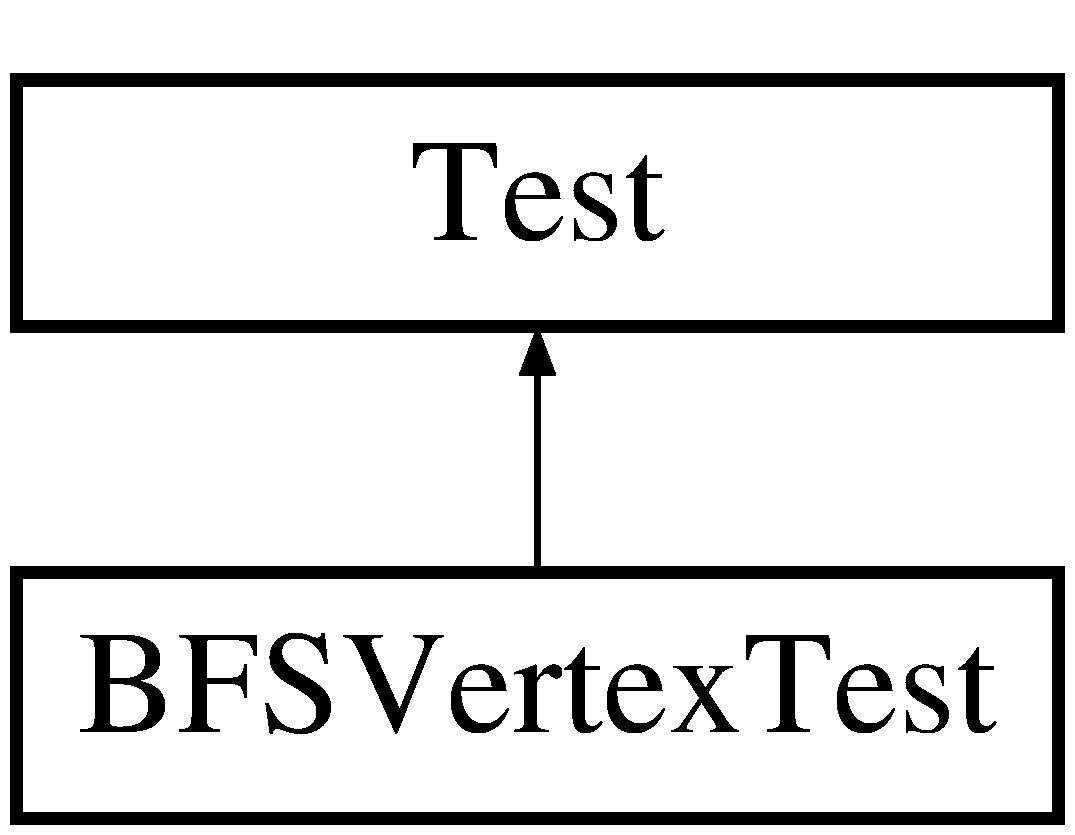
\includegraphics[height=2.000000cm]{class_b_f_s_vertex_test}
\end{center}
\end{figure}
\subsection*{Public Types}
\begin{DoxyCompactItemize}
\item 
typedef \hyperlink{class_b_f_s_vertex_test_a9ff4e5b50fe6468b08ee5e04f0527d7c}{B\+F\+S\+\_\+\+Vertex}$<$ double $>$ \hyperlink{class_b_f_s_vertex_test_a9ff4e5b50fe6468b08ee5e04f0527d7c}{B\+F\+S\+\_\+\+Vertex}
\end{DoxyCompactItemize}
\subsection*{Protected Member Functions}
\begin{DoxyCompactItemize}
\item 
void \hyperlink{class_b_f_s_vertex_test_a3f6d438f93bb897fc216d30a49718ce3}{Set\+Up} ()
\item 
void \hyperlink{class_b_f_s_vertex_test_a199a64fd9255e1f6908bb37da0fce740}{Tear\+Down} ()
\end{DoxyCompactItemize}
\subsection*{Protected Attributes}
\begin{DoxyCompactItemize}
\item 
std\+::shared\+\_\+ptr$<$ \hyperlink{class_b_f_s_vertex_test_a9ff4e5b50fe6468b08ee5e04f0527d7c}{B\+F\+S\+\_\+\+Vertex} $>$ \hyperlink{class_b_f_s_vertex_test_ab78f6c9cb070fe5a8992f61cc5f71920}{\+\_\+default\+\_\+vertex}
\item 
std\+::shared\+\_\+ptr$<$ \hyperlink{class_b_f_s_vertex_test_a9ff4e5b50fe6468b08ee5e04f0527d7c}{B\+F\+S\+\_\+\+Vertex} $>$ \hyperlink{class_b_f_s_vertex_test_aedd37204d4a3723bd78fa72af7caa6e0}{\+\_\+normal\+\_\+vertex}
\end{DoxyCompactItemize}


\subsection{Detailed Description}
\hyperlink{class_b_f_s_vertex_test}{B\+F\+S\+Vertex\+Test}\+:测试类,用于为测试提供基础数据 

{\ttfamily \hyperlink{class_b_f_s_vertex_test}{B\+F\+S\+Vertex\+Test}}是 {\ttfamily \+::testing\+::\+Test} 的子类。它主要用于为每一个{\ttfamily T\+E\+S\+T\+\_\+\+F}准备测试环境 

Definition at line 31 of file bfs\+\_\+vertex\+\_\+test.\+h.



\subsection{Member Typedef Documentation}
\hypertarget{class_b_f_s_vertex_test_a9ff4e5b50fe6468b08ee5e04f0527d7c}{}\index{B\+F\+S\+Vertex\+Test@{B\+F\+S\+Vertex\+Test}!B\+F\+S\+\_\+\+Vertex@{B\+F\+S\+\_\+\+Vertex}}
\index{B\+F\+S\+\_\+\+Vertex@{B\+F\+S\+\_\+\+Vertex}!B\+F\+S\+Vertex\+Test@{B\+F\+S\+Vertex\+Test}}
\subsubsection[{B\+F\+S\+\_\+\+Vertex}]{\setlength{\rightskip}{0pt plus 5cm}typedef {\bf B\+F\+S\+\_\+\+Vertex}$<$double$>$ {\bf B\+F\+S\+Vertex\+Test\+::\+B\+F\+S\+\_\+\+Vertex}}\label{class_b_f_s_vertex_test_a9ff4e5b50fe6468b08ee5e04f0527d7c}
模板实例化的顶点类型为{\ttfamily B\+F\+S\+\_\+\+Vertex$<$double$>$} 

Definition at line 34 of file bfs\+\_\+vertex\+\_\+test.\+h.



\subsection{Member Function Documentation}
\hypertarget{class_b_f_s_vertex_test_a3f6d438f93bb897fc216d30a49718ce3}{}\index{B\+F\+S\+Vertex\+Test@{B\+F\+S\+Vertex\+Test}!Set\+Up@{Set\+Up}}
\index{Set\+Up@{Set\+Up}!B\+F\+S\+Vertex\+Test@{B\+F\+S\+Vertex\+Test}}
\subsubsection[{Set\+Up()}]{\setlength{\rightskip}{0pt plus 5cm}void B\+F\+S\+Vertex\+Test\+::\+Set\+Up (
\begin{DoxyParamCaption}
{}
\end{DoxyParamCaption}
)\hspace{0.3cm}{\ttfamily [inline]}, {\ttfamily [protected]}}\label{class_b_f_s_vertex_test_a3f6d438f93bb897fc216d30a49718ce3}


Definition at line 37 of file bfs\+\_\+vertex\+\_\+test.\+h.

\hypertarget{class_b_f_s_vertex_test_a199a64fd9255e1f6908bb37da0fce740}{}\index{B\+F\+S\+Vertex\+Test@{B\+F\+S\+Vertex\+Test}!Tear\+Down@{Tear\+Down}}
\index{Tear\+Down@{Tear\+Down}!B\+F\+S\+Vertex\+Test@{B\+F\+S\+Vertex\+Test}}
\subsubsection[{Tear\+Down()}]{\setlength{\rightskip}{0pt plus 5cm}void B\+F\+S\+Vertex\+Test\+::\+Tear\+Down (
\begin{DoxyParamCaption}
{}
\end{DoxyParamCaption}
)\hspace{0.3cm}{\ttfamily [inline]}, {\ttfamily [protected]}}\label{class_b_f_s_vertex_test_a199a64fd9255e1f6908bb37da0fce740}


Definition at line 41 of file bfs\+\_\+vertex\+\_\+test.\+h.



\subsection{Member Data Documentation}
\hypertarget{class_b_f_s_vertex_test_ab78f6c9cb070fe5a8992f61cc5f71920}{}\index{B\+F\+S\+Vertex\+Test@{B\+F\+S\+Vertex\+Test}!\+\_\+default\+\_\+vertex@{\+\_\+default\+\_\+vertex}}
\index{\+\_\+default\+\_\+vertex@{\+\_\+default\+\_\+vertex}!B\+F\+S\+Vertex\+Test@{B\+F\+S\+Vertex\+Test}}
\subsubsection[{\+\_\+default\+\_\+vertex}]{\setlength{\rightskip}{0pt plus 5cm}std\+::shared\+\_\+ptr$<${\bf B\+F\+S\+\_\+\+Vertex}$>$ B\+F\+S\+Vertex\+Test\+::\+\_\+default\+\_\+vertex\hspace{0.3cm}{\ttfamily [protected]}}\label{class_b_f_s_vertex_test_ab78f6c9cb070fe5a8992f61cc5f71920}
指向一个默认构造的顶点 

Definition at line 42 of file bfs\+\_\+vertex\+\_\+test.\+h.

\hypertarget{class_b_f_s_vertex_test_aedd37204d4a3723bd78fa72af7caa6e0}{}\index{B\+F\+S\+Vertex\+Test@{B\+F\+S\+Vertex\+Test}!\+\_\+normal\+\_\+vertex@{\+\_\+normal\+\_\+vertex}}
\index{\+\_\+normal\+\_\+vertex@{\+\_\+normal\+\_\+vertex}!B\+F\+S\+Vertex\+Test@{B\+F\+S\+Vertex\+Test}}
\subsubsection[{\+\_\+normal\+\_\+vertex}]{\setlength{\rightskip}{0pt plus 5cm}std\+::shared\+\_\+ptr$<${\bf B\+F\+S\+\_\+\+Vertex}$>$ B\+F\+S\+Vertex\+Test\+::\+\_\+normal\+\_\+vertex\hspace{0.3cm}{\ttfamily [protected]}}\label{class_b_f_s_vertex_test_aedd37204d4a3723bd78fa72af7caa6e0}
指向一个显式构造的顶点 

Definition at line 43 of file bfs\+\_\+vertex\+\_\+test.\+h.



The documentation for this class was generated from the following file\+:\begin{DoxyCompactItemize}
\item 
src/graph\+\_\+algorithms/basic\+\_\+graph/graph\+\_\+representation/graph\+\_\+vertex/\hyperlink{bfs__vertex__test_8h}{bfs\+\_\+vertex\+\_\+test.\+h}\end{DoxyCompactItemize}

\hypertarget{struct_introduction_to_algorithm_1_1_tree_algorithm_1_1_binary_tree}{}\section{Introduction\+To\+Algorithm\+:\+:Tree\+Algorithm\+:\+:Binary\+Tree$<$ Node\+T $>$ Struct Template Reference}
\label{struct_introduction_to_algorithm_1_1_tree_algorithm_1_1_binary_tree}\index{Introduction\+To\+Algorithm\+::\+Tree\+Algorithm\+::\+Binary\+Tree$<$ Node\+T $>$@{Introduction\+To\+Algorithm\+::\+Tree\+Algorithm\+::\+Binary\+Tree$<$ Node\+T $>$}}


Binary\+Tree:二叉树,算法导论10章10.4节  




{\ttfamily \#include $<$binarytree.\+h$>$}

\subsection*{Public Types}
\begin{DoxyCompactItemize}
\item 
typedef Node\+T \hyperlink{struct_introduction_to_algorithm_1_1_tree_algorithm_1_1_binary_tree_a9a441f3f41c5b69758204ba60fe02010}{Node\+Type}
\item 
typedef Node\+T\+::\+Key\+Type \hyperlink{struct_introduction_to_algorithm_1_1_tree_algorithm_1_1_binary_tree_af231d881ec1d08492b2b5b5638e5e373}{Key\+Type}
\end{DoxyCompactItemize}
\subsection*{Public Member Functions}
\begin{DoxyCompactItemize}
\item 
\hyperlink{struct_introduction_to_algorithm_1_1_tree_algorithm_1_1_binary_tree_adc9b1c18fd12ab56de09e92005848abf}{Binary\+Tree} ()
\begin{DoxyCompactList}\small\item\em 默认函数 \end{DoxyCompactList}\item 
std\+::string \hyperlink{struct_introduction_to_algorithm_1_1_tree_algorithm_1_1_binary_tree_a96fa515f1c3b4176a03c37b8ea582339}{to\+\_\+xml} ()
\begin{DoxyCompactList}\small\item\em to\+\_\+xml\+:返回本树的{\ttfamily xml}描述。 \end{DoxyCompactList}\end{DoxyCompactItemize}
\subsection*{Public Attributes}
\begin{DoxyCompactItemize}
\item 
std\+::shared\+\_\+ptr$<$ \hyperlink{struct_introduction_to_algorithm_1_1_tree_algorithm_1_1_binary_tree_a9a441f3f41c5b69758204ba60fe02010}{Node\+Type} $>$ \hyperlink{struct_introduction_to_algorithm_1_1_tree_algorithm_1_1_binary_tree_aa0d43af70ef50ff59740dced2e832074}{root}
\end{DoxyCompactItemize}


\subsection{Detailed Description}
\subsubsection*{template$<$typename Node\+T$>$struct Introduction\+To\+Algorithm\+::\+Tree\+Algorithm\+::\+Binary\+Tree$<$ Node\+T $>$}

Binary\+Tree:二叉树,算法导论10章10.4节 

二叉树通过一个root(若引用)指向一个节点对象。当root为空时,树为空 

Definition at line 32 of file binarytree.\+h.



\subsection{Member Typedef Documentation}
\hypertarget{struct_introduction_to_algorithm_1_1_tree_algorithm_1_1_binary_tree_af231d881ec1d08492b2b5b5638e5e373}{}\index{Introduction\+To\+Algorithm\+::\+Tree\+Algorithm\+::\+Binary\+Tree@{Introduction\+To\+Algorithm\+::\+Tree\+Algorithm\+::\+Binary\+Tree}!Key\+Type@{Key\+Type}}
\index{Key\+Type@{Key\+Type}!Introduction\+To\+Algorithm\+::\+Tree\+Algorithm\+::\+Binary\+Tree@{Introduction\+To\+Algorithm\+::\+Tree\+Algorithm\+::\+Binary\+Tree}}
\subsubsection[{Key\+Type}]{\setlength{\rightskip}{0pt plus 5cm}template$<$typename Node\+T$>$ typedef Node\+T\+::\+Key\+Type {\bf Introduction\+To\+Algorithm\+::\+Tree\+Algorithm\+::\+Binary\+Tree}$<$ Node\+T $>$\+::{\bf Key\+Type}}\label{struct_introduction_to_algorithm_1_1_tree_algorithm_1_1_binary_tree_af231d881ec1d08492b2b5b5638e5e373}
树的节点存储数据的类型 

Definition at line 35 of file binarytree.\+h.

\hypertarget{struct_introduction_to_algorithm_1_1_tree_algorithm_1_1_binary_tree_a9a441f3f41c5b69758204ba60fe02010}{}\index{Introduction\+To\+Algorithm\+::\+Tree\+Algorithm\+::\+Binary\+Tree@{Introduction\+To\+Algorithm\+::\+Tree\+Algorithm\+::\+Binary\+Tree}!Node\+Type@{Node\+Type}}
\index{Node\+Type@{Node\+Type}!Introduction\+To\+Algorithm\+::\+Tree\+Algorithm\+::\+Binary\+Tree@{Introduction\+To\+Algorithm\+::\+Tree\+Algorithm\+::\+Binary\+Tree}}
\subsubsection[{Node\+Type}]{\setlength{\rightskip}{0pt plus 5cm}template$<$typename Node\+T$>$ typedef Node\+T {\bf Introduction\+To\+Algorithm\+::\+Tree\+Algorithm\+::\+Binary\+Tree}$<$ Node\+T $>$\+::{\bf Node\+Type}}\label{struct_introduction_to_algorithm_1_1_tree_algorithm_1_1_binary_tree_a9a441f3f41c5b69758204ba60fe02010}
树的节点类型 

Definition at line 34 of file binarytree.\+h.



\subsection{Constructor \& Destructor Documentation}
\hypertarget{struct_introduction_to_algorithm_1_1_tree_algorithm_1_1_binary_tree_adc9b1c18fd12ab56de09e92005848abf}{}\index{Introduction\+To\+Algorithm\+::\+Tree\+Algorithm\+::\+Binary\+Tree@{Introduction\+To\+Algorithm\+::\+Tree\+Algorithm\+::\+Binary\+Tree}!Binary\+Tree@{Binary\+Tree}}
\index{Binary\+Tree@{Binary\+Tree}!Introduction\+To\+Algorithm\+::\+Tree\+Algorithm\+::\+Binary\+Tree@{Introduction\+To\+Algorithm\+::\+Tree\+Algorithm\+::\+Binary\+Tree}}
\subsubsection[{Binary\+Tree()}]{\setlength{\rightskip}{0pt plus 5cm}template$<$typename Node\+T$>$ {\bf Introduction\+To\+Algorithm\+::\+Tree\+Algorithm\+::\+Binary\+Tree}$<$ Node\+T $>$\+::{\bf Binary\+Tree} (
\begin{DoxyParamCaption}
{}
\end{DoxyParamCaption}
)\hspace{0.3cm}{\ttfamily [inline]}}\label{struct_introduction_to_algorithm_1_1_tree_algorithm_1_1_binary_tree_adc9b1c18fd12ab56de09e92005848abf}


默认函数 

新建的二叉树默认为空 

Definition at line 41 of file binarytree.\+h.



\subsection{Member Function Documentation}
\hypertarget{struct_introduction_to_algorithm_1_1_tree_algorithm_1_1_binary_tree_a96fa515f1c3b4176a03c37b8ea582339}{}\index{Introduction\+To\+Algorithm\+::\+Tree\+Algorithm\+::\+Binary\+Tree@{Introduction\+To\+Algorithm\+::\+Tree\+Algorithm\+::\+Binary\+Tree}!to\+\_\+xml@{to\+\_\+xml}}
\index{to\+\_\+xml@{to\+\_\+xml}!Introduction\+To\+Algorithm\+::\+Tree\+Algorithm\+::\+Binary\+Tree@{Introduction\+To\+Algorithm\+::\+Tree\+Algorithm\+::\+Binary\+Tree}}
\subsubsection[{to\+\_\+xml()}]{\setlength{\rightskip}{0pt plus 5cm}template$<$typename Node\+T$>$ std\+::string {\bf Introduction\+To\+Algorithm\+::\+Tree\+Algorithm\+::\+Binary\+Tree}$<$ Node\+T $>$\+::to\+\_\+xml (
\begin{DoxyParamCaption}
{}
\end{DoxyParamCaption}
)\hspace{0.3cm}{\ttfamily [inline]}}\label{struct_introduction_to_algorithm_1_1_tree_algorithm_1_1_binary_tree_a96fa515f1c3b4176a03c37b8ea582339}


to\+\_\+xml\+:返回本树的{\ttfamily xml}描述。 

\begin{DoxyReturn}{Returns}
\+: 树的{\ttfamily xml}描述的字符串
\end{DoxyReturn}
该函数获取本树的{\ttfamily xml}描述 

Definition at line 51 of file binarytree.\+h.



\subsection{Member Data Documentation}
\hypertarget{struct_introduction_to_algorithm_1_1_tree_algorithm_1_1_binary_tree_aa0d43af70ef50ff59740dced2e832074}{}\index{Introduction\+To\+Algorithm\+::\+Tree\+Algorithm\+::\+Binary\+Tree@{Introduction\+To\+Algorithm\+::\+Tree\+Algorithm\+::\+Binary\+Tree}!root@{root}}
\index{root@{root}!Introduction\+To\+Algorithm\+::\+Tree\+Algorithm\+::\+Binary\+Tree@{Introduction\+To\+Algorithm\+::\+Tree\+Algorithm\+::\+Binary\+Tree}}
\subsubsection[{root}]{\setlength{\rightskip}{0pt plus 5cm}template$<$typename Node\+T$>$ std\+::shared\+\_\+ptr$<${\bf Node\+Type}$>$ {\bf Introduction\+To\+Algorithm\+::\+Tree\+Algorithm\+::\+Binary\+Tree}$<$ Node\+T $>$\+::root}\label{struct_introduction_to_algorithm_1_1_tree_algorithm_1_1_binary_tree_aa0d43af70ef50ff59740dced2e832074}
树的根节点,时一个指向节点对象的强引用 

Definition at line 59 of file binarytree.\+h.



The documentation for this struct was generated from the following file\+:\begin{DoxyCompactItemize}
\item 
src/tree\+\_\+algorithms/binarytree/\hyperlink{binarytree_8h}{binarytree.\+h}\end{DoxyCompactItemize}

\hypertarget{struct_introduction_to_algorithm_1_1_tree_algorithm_1_1_binary_tree_node}{}\section{Introduction\+To\+Algorithm\+:\+:Tree\+Algorithm\+:\+:Binary\+Tree\+Node$<$ K\+Type $>$ Struct Template Reference}
\label{struct_introduction_to_algorithm_1_1_tree_algorithm_1_1_binary_tree_node}\index{Introduction\+To\+Algorithm\+::\+Tree\+Algorithm\+::\+Binary\+Tree\+Node$<$ K\+Type $>$@{Introduction\+To\+Algorithm\+::\+Tree\+Algorithm\+::\+Binary\+Tree\+Node$<$ K\+Type $>$}}


Binary\+Tree\+Node:二叉树的节点,算法导论xx章xx节  




{\ttfamily \#include $<$binarytreenode.\+h$>$}

\subsection*{Public Types}
\begin{DoxyCompactItemize}
\item 
typedef K\+Type \hyperlink{struct_introduction_to_algorithm_1_1_tree_algorithm_1_1_binary_tree_node_adbd8539e7a907c3a8fe7a8b79e7032e8}{Key\+Type}
\end{DoxyCompactItemize}
\subsection*{Public Member Functions}
\begin{DoxyCompactItemize}
\item 
\hyperlink{struct_introduction_to_algorithm_1_1_tree_algorithm_1_1_binary_tree_node_a8e8de673785852b0c091916f5fb64e78}{Binary\+Tree\+Node} ()
\begin{DoxyCompactList}\small\item\em 默认构造函数 \end{DoxyCompactList}\item 
\hyperlink{struct_introduction_to_algorithm_1_1_tree_algorithm_1_1_binary_tree_node_a8382a5ddc6f9c8cbfeacd0f0163d8c4d}{Binary\+Tree\+Node} (const \hyperlink{struct_introduction_to_algorithm_1_1_tree_algorithm_1_1_binary_tree_node_adbd8539e7a907c3a8fe7a8b79e7032e8}{Key\+Type} \&keyvalue)
\begin{DoxyCompactList}\small\item\em 显式构造函数 \end{DoxyCompactList}\item 
virtual std\+::string \hyperlink{struct_introduction_to_algorithm_1_1_tree_algorithm_1_1_binary_tree_node_ae552fb23243e499a60ef73375fabe239}{to\+\_\+string} ()
\begin{DoxyCompactList}\small\item\em to\+\_\+string\+:返回该节点的字符串描述 \end{DoxyCompactList}\item 
virtual std\+::string \hyperlink{struct_introduction_to_algorithm_1_1_tree_algorithm_1_1_binary_tree_node_a694d14f0b33f2f052f11148ecbe1684e}{to\+\_\+xml} ()
\begin{DoxyCompactList}\small\item\em to\+\_\+xml\+:返回以该节点为根的子树的{\ttfamily xml}描述。 \end{DoxyCompactList}\item 
bool \hyperlink{struct_introduction_to_algorithm_1_1_tree_algorithm_1_1_binary_tree_node_a54a90606ceb604a1a4d01056429a8a06}{is\+\_\+left\+\_\+child} ()
\begin{DoxyCompactList}\small\item\em is\+\_\+left\+\_\+child\+:判断本节点是否左子节点。 \end{DoxyCompactList}\item 
bool \hyperlink{struct_introduction_to_algorithm_1_1_tree_algorithm_1_1_binary_tree_node_a34c1912a2a7e9caa7a67354218fd7640}{is\+\_\+right\+\_\+child} ()
\begin{DoxyCompactList}\small\item\em is\+\_\+right\+\_\+child\+:判断本节点是否右子节点。 \end{DoxyCompactList}\end{DoxyCompactItemize}
\subsection*{Public Attributes}
\begin{DoxyCompactItemize}
\item 
std\+::weak\+\_\+ptr$<$ \hyperlink{struct_introduction_to_algorithm_1_1_tree_algorithm_1_1_binary_tree_node}{Binary\+Tree\+Node} $>$ \hyperlink{struct_introduction_to_algorithm_1_1_tree_algorithm_1_1_binary_tree_node_aa94cbc785416ba74505661baac55a9fd}{parent}
\item 
std\+::shared\+\_\+ptr$<$ \hyperlink{struct_introduction_to_algorithm_1_1_tree_algorithm_1_1_binary_tree_node}{Binary\+Tree\+Node} $>$ \hyperlink{struct_introduction_to_algorithm_1_1_tree_algorithm_1_1_binary_tree_node_a3e056b1d34820497ac3a23a16180be2b}{lchild}
\item 
std\+::shared\+\_\+ptr$<$ \hyperlink{struct_introduction_to_algorithm_1_1_tree_algorithm_1_1_binary_tree_node}{Binary\+Tree\+Node} $>$ \hyperlink{struct_introduction_to_algorithm_1_1_tree_algorithm_1_1_binary_tree_node_aaccc444db582ed362bff4e50efbc47c7}{rchild}
\item 
\hyperlink{struct_introduction_to_algorithm_1_1_tree_algorithm_1_1_binary_tree_node_adbd8539e7a907c3a8fe7a8b79e7032e8}{Key\+Type} \hyperlink{struct_introduction_to_algorithm_1_1_tree_algorithm_1_1_binary_tree_node_af3cb8030ab05ccaf1a69a86c9f468b8d}{key}
\end{DoxyCompactItemize}


\subsection{Detailed Description}
\subsubsection*{template$<$typename K\+Type$>$struct Introduction\+To\+Algorithm\+::\+Tree\+Algorithm\+::\+Binary\+Tree\+Node$<$ K\+Type $>$}

Binary\+Tree\+Node:二叉树的节点,算法导论xx章xx节 

任何一个节点都有两个强引用指向左右子节点,以及一个弱引用指向它的父节点。节点还有一个{\ttfamily key}成员包含具体的数据 

Definition at line 31 of file binarytreenode.\+h.



\subsection{Member Typedef Documentation}
\hypertarget{struct_introduction_to_algorithm_1_1_tree_algorithm_1_1_binary_tree_node_adbd8539e7a907c3a8fe7a8b79e7032e8}{}\index{Introduction\+To\+Algorithm\+::\+Tree\+Algorithm\+::\+Binary\+Tree\+Node@{Introduction\+To\+Algorithm\+::\+Tree\+Algorithm\+::\+Binary\+Tree\+Node}!Key\+Type@{Key\+Type}}
\index{Key\+Type@{Key\+Type}!Introduction\+To\+Algorithm\+::\+Tree\+Algorithm\+::\+Binary\+Tree\+Node@{Introduction\+To\+Algorithm\+::\+Tree\+Algorithm\+::\+Binary\+Tree\+Node}}
\subsubsection[{Key\+Type}]{\setlength{\rightskip}{0pt plus 5cm}template$<$typename K\+Type $>$ typedef K\+Type {\bf Introduction\+To\+Algorithm\+::\+Tree\+Algorithm\+::\+Binary\+Tree\+Node}$<$ K\+Type $>$\+::{\bf Key\+Type}}\label{struct_introduction_to_algorithm_1_1_tree_algorithm_1_1_binary_tree_node_adbd8539e7a907c3a8fe7a8b79e7032e8}
节点保存的数据的类型 

Definition at line 34 of file binarytreenode.\+h.



\subsection{Constructor \& Destructor Documentation}
\hypertarget{struct_introduction_to_algorithm_1_1_tree_algorithm_1_1_binary_tree_node_a8e8de673785852b0c091916f5fb64e78}{}\index{Introduction\+To\+Algorithm\+::\+Tree\+Algorithm\+::\+Binary\+Tree\+Node@{Introduction\+To\+Algorithm\+::\+Tree\+Algorithm\+::\+Binary\+Tree\+Node}!Binary\+Tree\+Node@{Binary\+Tree\+Node}}
\index{Binary\+Tree\+Node@{Binary\+Tree\+Node}!Introduction\+To\+Algorithm\+::\+Tree\+Algorithm\+::\+Binary\+Tree\+Node@{Introduction\+To\+Algorithm\+::\+Tree\+Algorithm\+::\+Binary\+Tree\+Node}}
\subsubsection[{Binary\+Tree\+Node()}]{\setlength{\rightskip}{0pt plus 5cm}template$<$typename K\+Type $>$ {\bf Introduction\+To\+Algorithm\+::\+Tree\+Algorithm\+::\+Binary\+Tree\+Node}$<$ K\+Type $>$\+::{\bf Binary\+Tree\+Node} (
\begin{DoxyParamCaption}
{}
\end{DoxyParamCaption}
)\hspace{0.3cm}{\ttfamily [inline]}}\label{struct_introduction_to_algorithm_1_1_tree_algorithm_1_1_binary_tree_node_a8e8de673785852b0c091916f5fb64e78}


默认构造函数 

所有的成员变量都采取默认值 

Definition at line 39 of file binarytreenode.\+h.

\hypertarget{struct_introduction_to_algorithm_1_1_tree_algorithm_1_1_binary_tree_node_a8382a5ddc6f9c8cbfeacd0f0163d8c4d}{}\index{Introduction\+To\+Algorithm\+::\+Tree\+Algorithm\+::\+Binary\+Tree\+Node@{Introduction\+To\+Algorithm\+::\+Tree\+Algorithm\+::\+Binary\+Tree\+Node}!Binary\+Tree\+Node@{Binary\+Tree\+Node}}
\index{Binary\+Tree\+Node@{Binary\+Tree\+Node}!Introduction\+To\+Algorithm\+::\+Tree\+Algorithm\+::\+Binary\+Tree\+Node@{Introduction\+To\+Algorithm\+::\+Tree\+Algorithm\+::\+Binary\+Tree\+Node}}
\subsubsection[{Binary\+Tree\+Node(const Key\+Type \&keyvalue)}]{\setlength{\rightskip}{0pt plus 5cm}template$<$typename K\+Type $>$ {\bf Introduction\+To\+Algorithm\+::\+Tree\+Algorithm\+::\+Binary\+Tree\+Node}$<$ K\+Type $>$\+::{\bf Binary\+Tree\+Node} (
\begin{DoxyParamCaption}
\item[{const {\bf Key\+Type} \&}]{keyvalue}
\end{DoxyParamCaption}
)\hspace{0.3cm}{\ttfamily [inline]}, {\ttfamily [explicit]}}\label{struct_introduction_to_algorithm_1_1_tree_algorithm_1_1_binary_tree_node_a8382a5ddc6f9c8cbfeacd0f0163d8c4d}


显式构造函数 


\begin{DoxyParams}{Parameters}
{\em keyvalue\+:节点要保存的数据内容} & 指定{\ttfamily key}成员需要赋值的数据 \\
\hline
\end{DoxyParams}


Definition at line 48 of file binarytreenode.\+h.



\subsection{Member Function Documentation}
\hypertarget{struct_introduction_to_algorithm_1_1_tree_algorithm_1_1_binary_tree_node_a54a90606ceb604a1a4d01056429a8a06}{}\index{Introduction\+To\+Algorithm\+::\+Tree\+Algorithm\+::\+Binary\+Tree\+Node@{Introduction\+To\+Algorithm\+::\+Tree\+Algorithm\+::\+Binary\+Tree\+Node}!is\+\_\+left\+\_\+child@{is\+\_\+left\+\_\+child}}
\index{is\+\_\+left\+\_\+child@{is\+\_\+left\+\_\+child}!Introduction\+To\+Algorithm\+::\+Tree\+Algorithm\+::\+Binary\+Tree\+Node@{Introduction\+To\+Algorithm\+::\+Tree\+Algorithm\+::\+Binary\+Tree\+Node}}
\subsubsection[{is\+\_\+left\+\_\+child()}]{\setlength{\rightskip}{0pt plus 5cm}template$<$typename K\+Type $>$ bool {\bf Introduction\+To\+Algorithm\+::\+Tree\+Algorithm\+::\+Binary\+Tree\+Node}$<$ K\+Type $>$\+::is\+\_\+left\+\_\+child (
\begin{DoxyParamCaption}
{}
\end{DoxyParamCaption}
)\hspace{0.3cm}{\ttfamily [inline]}}\label{struct_introduction_to_algorithm_1_1_tree_algorithm_1_1_binary_tree_node_a54a90606ceb604a1a4d01056429a8a06}


is\+\_\+left\+\_\+child\+:判断本节点是否左子节点。 

\begin{DoxyReturn}{Returns}
返回{\ttfamily true}或者{\ttfamily false} 该函数判断本节点是否是左子节点。如果本节点的父节点为空,则返回{\ttfamily false};如果本节点的父节点非空且本节点是父节点的左子节点,则返回{\ttfamily true};否则返回{\ttfamily false} 
\end{DoxyReturn}


Definition at line 99 of file binarytreenode.\+h.

\hypertarget{struct_introduction_to_algorithm_1_1_tree_algorithm_1_1_binary_tree_node_a34c1912a2a7e9caa7a67354218fd7640}{}\index{Introduction\+To\+Algorithm\+::\+Tree\+Algorithm\+::\+Binary\+Tree\+Node@{Introduction\+To\+Algorithm\+::\+Tree\+Algorithm\+::\+Binary\+Tree\+Node}!is\+\_\+right\+\_\+child@{is\+\_\+right\+\_\+child}}
\index{is\+\_\+right\+\_\+child@{is\+\_\+right\+\_\+child}!Introduction\+To\+Algorithm\+::\+Tree\+Algorithm\+::\+Binary\+Tree\+Node@{Introduction\+To\+Algorithm\+::\+Tree\+Algorithm\+::\+Binary\+Tree\+Node}}
\subsubsection[{is\+\_\+right\+\_\+child()}]{\setlength{\rightskip}{0pt plus 5cm}template$<$typename K\+Type $>$ bool {\bf Introduction\+To\+Algorithm\+::\+Tree\+Algorithm\+::\+Binary\+Tree\+Node}$<$ K\+Type $>$\+::is\+\_\+right\+\_\+child (
\begin{DoxyParamCaption}
{}
\end{DoxyParamCaption}
)\hspace{0.3cm}{\ttfamily [inline]}}\label{struct_introduction_to_algorithm_1_1_tree_algorithm_1_1_binary_tree_node_a34c1912a2a7e9caa7a67354218fd7640}


is\+\_\+right\+\_\+child\+:判断本节点是否右子节点。 

\begin{DoxyReturn}{Returns}
返回{\ttfamily true}或者{\ttfamily false} 该函数判断本节点是否是右子节点。如果本节点的父节点为空,则返回{\ttfamily false};如果本节点的父节点非空且本节点是父节点的右子节点,则返回{\ttfamily true};否则返回{\ttfamily false} 
\end{DoxyReturn}


Definition at line 113 of file binarytreenode.\+h.

\hypertarget{struct_introduction_to_algorithm_1_1_tree_algorithm_1_1_binary_tree_node_ae552fb23243e499a60ef73375fabe239}{}\index{Introduction\+To\+Algorithm\+::\+Tree\+Algorithm\+::\+Binary\+Tree\+Node@{Introduction\+To\+Algorithm\+::\+Tree\+Algorithm\+::\+Binary\+Tree\+Node}!to\+\_\+string@{to\+\_\+string}}
\index{to\+\_\+string@{to\+\_\+string}!Introduction\+To\+Algorithm\+::\+Tree\+Algorithm\+::\+Binary\+Tree\+Node@{Introduction\+To\+Algorithm\+::\+Tree\+Algorithm\+::\+Binary\+Tree\+Node}}
\subsubsection[{to\+\_\+string()}]{\setlength{\rightskip}{0pt plus 5cm}template$<$typename K\+Type $>$ virtual std\+::string {\bf Introduction\+To\+Algorithm\+::\+Tree\+Algorithm\+::\+Binary\+Tree\+Node}$<$ K\+Type $>$\+::to\+\_\+string (
\begin{DoxyParamCaption}
{}
\end{DoxyParamCaption}
)\hspace{0.3cm}{\ttfamily [inline]}, {\ttfamily [virtual]}}\label{struct_introduction_to_algorithm_1_1_tree_algorithm_1_1_binary_tree_node_ae552fb23243e499a60ef73375fabe239}


to\+\_\+string\+:返回该节点的字符串描述 

\begin{DoxyReturn}{Returns}
\+: 本节点的描述字符串
\end{DoxyReturn}
该函数打印本节点的{\ttfamily key},以及父节点(若存在)、子节点(若存在)的{\ttfamily key} 

Definition at line 58 of file binarytreenode.\+h.

\hypertarget{struct_introduction_to_algorithm_1_1_tree_algorithm_1_1_binary_tree_node_a694d14f0b33f2f052f11148ecbe1684e}{}\index{Introduction\+To\+Algorithm\+::\+Tree\+Algorithm\+::\+Binary\+Tree\+Node@{Introduction\+To\+Algorithm\+::\+Tree\+Algorithm\+::\+Binary\+Tree\+Node}!to\+\_\+xml@{to\+\_\+xml}}
\index{to\+\_\+xml@{to\+\_\+xml}!Introduction\+To\+Algorithm\+::\+Tree\+Algorithm\+::\+Binary\+Tree\+Node@{Introduction\+To\+Algorithm\+::\+Tree\+Algorithm\+::\+Binary\+Tree\+Node}}
\subsubsection[{to\+\_\+xml()}]{\setlength{\rightskip}{0pt plus 5cm}template$<$typename K\+Type $>$ virtual std\+::string {\bf Introduction\+To\+Algorithm\+::\+Tree\+Algorithm\+::\+Binary\+Tree\+Node}$<$ K\+Type $>$\+::to\+\_\+xml (
\begin{DoxyParamCaption}
{}
\end{DoxyParamCaption}
)\hspace{0.3cm}{\ttfamily [inline]}, {\ttfamily [virtual]}}\label{struct_introduction_to_algorithm_1_1_tree_algorithm_1_1_binary_tree_node_a694d14f0b33f2f052f11148ecbe1684e}


to\+\_\+xml\+:返回以该节点为根的子树的{\ttfamily xml}描述。 

\begin{DoxyReturn}{Returns}
\+: 本节点子树的{\ttfamily xml}描述的字符串
\end{DoxyReturn}
该函数返回以本节点为根的子树的{\ttfamily xml}描述。对子节点递归调用从而生成{\ttfamily xml}数据 

Definition at line 79 of file binarytreenode.\+h.



\subsection{Member Data Documentation}
\hypertarget{struct_introduction_to_algorithm_1_1_tree_algorithm_1_1_binary_tree_node_af3cb8030ab05ccaf1a69a86c9f468b8d}{}\index{Introduction\+To\+Algorithm\+::\+Tree\+Algorithm\+::\+Binary\+Tree\+Node@{Introduction\+To\+Algorithm\+::\+Tree\+Algorithm\+::\+Binary\+Tree\+Node}!key@{key}}
\index{key@{key}!Introduction\+To\+Algorithm\+::\+Tree\+Algorithm\+::\+Binary\+Tree\+Node@{Introduction\+To\+Algorithm\+::\+Tree\+Algorithm\+::\+Binary\+Tree\+Node}}
\subsubsection[{key}]{\setlength{\rightskip}{0pt plus 5cm}template$<$typename K\+Type $>$ {\bf Key\+Type} {\bf Introduction\+To\+Algorithm\+::\+Tree\+Algorithm\+::\+Binary\+Tree\+Node}$<$ K\+Type $>$\+::key}\label{struct_introduction_to_algorithm_1_1_tree_algorithm_1_1_binary_tree_node_af3cb8030ab05ccaf1a69a86c9f468b8d}
节点的保存的数据 

Definition at line 125 of file binarytreenode.\+h.

\hypertarget{struct_introduction_to_algorithm_1_1_tree_algorithm_1_1_binary_tree_node_a3e056b1d34820497ac3a23a16180be2b}{}\index{Introduction\+To\+Algorithm\+::\+Tree\+Algorithm\+::\+Binary\+Tree\+Node@{Introduction\+To\+Algorithm\+::\+Tree\+Algorithm\+::\+Binary\+Tree\+Node}!lchild@{lchild}}
\index{lchild@{lchild}!Introduction\+To\+Algorithm\+::\+Tree\+Algorithm\+::\+Binary\+Tree\+Node@{Introduction\+To\+Algorithm\+::\+Tree\+Algorithm\+::\+Binary\+Tree\+Node}}
\subsubsection[{lchild}]{\setlength{\rightskip}{0pt plus 5cm}template$<$typename K\+Type $>$ std\+::shared\+\_\+ptr$<${\bf Binary\+Tree\+Node}$>$ {\bf Introduction\+To\+Algorithm\+::\+Tree\+Algorithm\+::\+Binary\+Tree\+Node}$<$ K\+Type $>$\+::lchild}\label{struct_introduction_to_algorithm_1_1_tree_algorithm_1_1_binary_tree_node_a3e056b1d34820497ac3a23a16180be2b}
节点的左子节点的强引用 

Definition at line 123 of file binarytreenode.\+h.

\hypertarget{struct_introduction_to_algorithm_1_1_tree_algorithm_1_1_binary_tree_node_aa94cbc785416ba74505661baac55a9fd}{}\index{Introduction\+To\+Algorithm\+::\+Tree\+Algorithm\+::\+Binary\+Tree\+Node@{Introduction\+To\+Algorithm\+::\+Tree\+Algorithm\+::\+Binary\+Tree\+Node}!parent@{parent}}
\index{parent@{parent}!Introduction\+To\+Algorithm\+::\+Tree\+Algorithm\+::\+Binary\+Tree\+Node@{Introduction\+To\+Algorithm\+::\+Tree\+Algorithm\+::\+Binary\+Tree\+Node}}
\subsubsection[{parent}]{\setlength{\rightskip}{0pt plus 5cm}template$<$typename K\+Type $>$ std\+::weak\+\_\+ptr$<${\bf Binary\+Tree\+Node}$>$ {\bf Introduction\+To\+Algorithm\+::\+Tree\+Algorithm\+::\+Binary\+Tree\+Node}$<$ K\+Type $>$\+::parent}\label{struct_introduction_to_algorithm_1_1_tree_algorithm_1_1_binary_tree_node_aa94cbc785416ba74505661baac55a9fd}
节点的父节点的弱引用 

Definition at line 122 of file binarytreenode.\+h.

\hypertarget{struct_introduction_to_algorithm_1_1_tree_algorithm_1_1_binary_tree_node_aaccc444db582ed362bff4e50efbc47c7}{}\index{Introduction\+To\+Algorithm\+::\+Tree\+Algorithm\+::\+Binary\+Tree\+Node@{Introduction\+To\+Algorithm\+::\+Tree\+Algorithm\+::\+Binary\+Tree\+Node}!rchild@{rchild}}
\index{rchild@{rchild}!Introduction\+To\+Algorithm\+::\+Tree\+Algorithm\+::\+Binary\+Tree\+Node@{Introduction\+To\+Algorithm\+::\+Tree\+Algorithm\+::\+Binary\+Tree\+Node}}
\subsubsection[{rchild}]{\setlength{\rightskip}{0pt plus 5cm}template$<$typename K\+Type $>$ std\+::shared\+\_\+ptr$<${\bf Binary\+Tree\+Node}$>$ {\bf Introduction\+To\+Algorithm\+::\+Tree\+Algorithm\+::\+Binary\+Tree\+Node}$<$ K\+Type $>$\+::rchild}\label{struct_introduction_to_algorithm_1_1_tree_algorithm_1_1_binary_tree_node_aaccc444db582ed362bff4e50efbc47c7}
节点的右子节点的强引用 

Definition at line 124 of file binarytreenode.\+h.



The documentation for this struct was generated from the following file\+:\begin{DoxyCompactItemize}
\item 
src/tree\+\_\+algorithms/binarytreenode/\hyperlink{binarytreenode_8h}{binarytreenode.\+h}\end{DoxyCompactItemize}

\hypertarget{class_binary_tree_node_test}{}\section{Binary\+Tree\+Node\+Test Class Reference}
\label{class_binary_tree_node_test}\index{Binary\+Tree\+Node\+Test@{Binary\+Tree\+Node\+Test}}


\hyperlink{class_binary_tree_node_test}{Binary\+Tree\+Node\+Test}\+:测试类,用于为测试提供基础数据  




{\ttfamily \#include $<$binarytreenode\+\_\+test.\+h$>$}

Inheritance diagram for Binary\+Tree\+Node\+Test\+:\begin{figure}[H]
\begin{center}
\leavevmode
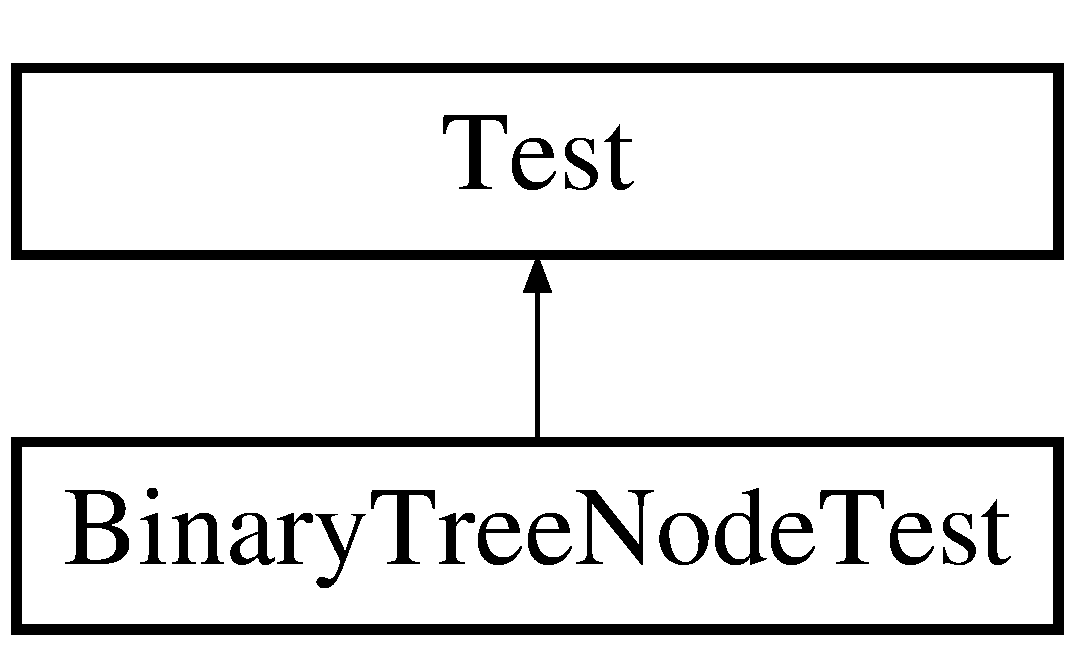
\includegraphics[height=2.000000cm]{class_binary_tree_node_test}
\end{center}
\end{figure}
\subsection*{Public Types}
\begin{DoxyCompactItemize}
\item 
typedef \hyperlink{struct_introduction_to_algorithm_1_1_tree_algorithm_1_1_binary_tree_node}{Binary\+Tree\+Node}$<$ int $>$ \hyperlink{class_binary_tree_node_test_aa8508b87ef3554a5dd1069a460f38679}{Node}
\end{DoxyCompactItemize}
\subsection*{Protected Member Functions}
\begin{DoxyCompactItemize}
\item 
void \hyperlink{class_binary_tree_node_test_a60ff0f181a5e3a45742949b1948b8095}{Set\+Up} ()
\item 
void \hyperlink{class_binary_tree_node_test_a93cbc74d7d46635510578aefa62ceca5}{Tear\+Down} ()
\end{DoxyCompactItemize}
\subsection*{Protected Attributes}
\begin{DoxyCompactItemize}
\item 
std\+::shared\+\_\+ptr$<$ \hyperlink{class_binary_tree_node_test_aa8508b87ef3554a5dd1069a460f38679}{Node} $>$ \hyperlink{class_binary_tree_node_test_af2db7bcee955bff2d4d2aa815a09b329}{default\+\_\+node}
\item 
std\+::shared\+\_\+ptr$<$ \hyperlink{class_binary_tree_node_test_aa8508b87ef3554a5dd1069a460f38679}{Node} $>$ \hyperlink{class_binary_tree_node_test_a07aad40489fc19ed29863c82a6c14863}{root\+\_\+node}
\end{DoxyCompactItemize}


\subsection{Detailed Description}
\hyperlink{class_binary_tree_node_test}{Binary\+Tree\+Node\+Test}\+:测试类,用于为测试提供基础数据 

{\ttfamily \hyperlink{class_binary_tree_node_test}{Binary\+Tree\+Node\+Test}}是 {\ttfamily \+::testing\+::\+Test} 的子类。它主要用于为每一个{\ttfamily T\+E\+S\+T\+\_\+\+F}准备测试环境 

Definition at line 29 of file binarytreenode\+\_\+test.\+h.



\subsection{Member Typedef Documentation}
\hypertarget{class_binary_tree_node_test_aa8508b87ef3554a5dd1069a460f38679}{}\index{Binary\+Tree\+Node\+Test@{Binary\+Tree\+Node\+Test}!Node@{Node}}
\index{Node@{Node}!Binary\+Tree\+Node\+Test@{Binary\+Tree\+Node\+Test}}
\subsubsection[{Node}]{\setlength{\rightskip}{0pt plus 5cm}typedef {\bf Binary\+Tree\+Node}$<$int$>$ {\bf Binary\+Tree\+Node\+Test\+::\+Node}}\label{class_binary_tree_node_test_aa8508b87ef3554a5dd1069a460f38679}


Definition at line 32 of file binarytreenode\+\_\+test.\+h.



\subsection{Member Function Documentation}
\hypertarget{class_binary_tree_node_test_a60ff0f181a5e3a45742949b1948b8095}{}\index{Binary\+Tree\+Node\+Test@{Binary\+Tree\+Node\+Test}!Set\+Up@{Set\+Up}}
\index{Set\+Up@{Set\+Up}!Binary\+Tree\+Node\+Test@{Binary\+Tree\+Node\+Test}}
\subsubsection[{Set\+Up()}]{\setlength{\rightskip}{0pt plus 5cm}void Binary\+Tree\+Node\+Test\+::\+Set\+Up (
\begin{DoxyParamCaption}
{}
\end{DoxyParamCaption}
)\hspace{0.3cm}{\ttfamily [inline]}, {\ttfamily [protected]}}\label{class_binary_tree_node_test_a60ff0f181a5e3a45742949b1948b8095}


Definition at line 34 of file binarytreenode\+\_\+test.\+h.

\hypertarget{class_binary_tree_node_test_a93cbc74d7d46635510578aefa62ceca5}{}\index{Binary\+Tree\+Node\+Test@{Binary\+Tree\+Node\+Test}!Tear\+Down@{Tear\+Down}}
\index{Tear\+Down@{Tear\+Down}!Binary\+Tree\+Node\+Test@{Binary\+Tree\+Node\+Test}}
\subsubsection[{Tear\+Down()}]{\setlength{\rightskip}{0pt plus 5cm}void Binary\+Tree\+Node\+Test\+::\+Tear\+Down (
\begin{DoxyParamCaption}
{}
\end{DoxyParamCaption}
)\hspace{0.3cm}{\ttfamily [inline]}, {\ttfamily [protected]}}\label{class_binary_tree_node_test_a93cbc74d7d46635510578aefa62ceca5}


Definition at line 43 of file binarytreenode\+\_\+test.\+h.



\subsection{Member Data Documentation}
\hypertarget{class_binary_tree_node_test_af2db7bcee955bff2d4d2aa815a09b329}{}\index{Binary\+Tree\+Node\+Test@{Binary\+Tree\+Node\+Test}!default\+\_\+node@{default\+\_\+node}}
\index{default\+\_\+node@{default\+\_\+node}!Binary\+Tree\+Node\+Test@{Binary\+Tree\+Node\+Test}}
\subsubsection[{default\+\_\+node}]{\setlength{\rightskip}{0pt plus 5cm}std\+::shared\+\_\+ptr$<${\bf Node}$>$ Binary\+Tree\+Node\+Test\+::default\+\_\+node\hspace{0.3cm}{\ttfamily [protected]}}\label{class_binary_tree_node_test_af2db7bcee955bff2d4d2aa815a09b329}
指向一个默认构造的结点 

Definition at line 46 of file binarytreenode\+\_\+test.\+h.

\hypertarget{class_binary_tree_node_test_a07aad40489fc19ed29863c82a6c14863}{}\index{Binary\+Tree\+Node\+Test@{Binary\+Tree\+Node\+Test}!root\+\_\+node@{root\+\_\+node}}
\index{root\+\_\+node@{root\+\_\+node}!Binary\+Tree\+Node\+Test@{Binary\+Tree\+Node\+Test}}
\subsubsection[{root\+\_\+node}]{\setlength{\rightskip}{0pt plus 5cm}std\+::shared\+\_\+ptr$<${\bf Node}$>$ Binary\+Tree\+Node\+Test\+::root\+\_\+node\hspace{0.3cm}{\ttfamily [protected]}}\label{class_binary_tree_node_test_a07aad40489fc19ed29863c82a6c14863}
指向一个非默认构造的结点 

Definition at line 47 of file binarytreenode\+\_\+test.\+h.



The documentation for this class was generated from the following file\+:\begin{DoxyCompactItemize}
\item 
src/tree\+\_\+algorithms/binarytreenode/\hyperlink{binarytreenode__test_8h}{binarytreenode\+\_\+test.\+h}\end{DoxyCompactItemize}

\hypertarget{class_binary_tree_test}{}\section{Binary\+Tree\+Test Class Reference}
\label{class_binary_tree_test}\index{Binary\+Tree\+Test@{Binary\+Tree\+Test}}


\hyperlink{class_binary_tree_test}{Binary\+Tree\+Test}\+:测试类,用于为测试提供基础数据  




{\ttfamily \#include $<$binarytree\+\_\+test.\+h$>$}

Inheritance diagram for Binary\+Tree\+Test\+:\begin{figure}[H]
\begin{center}
\leavevmode
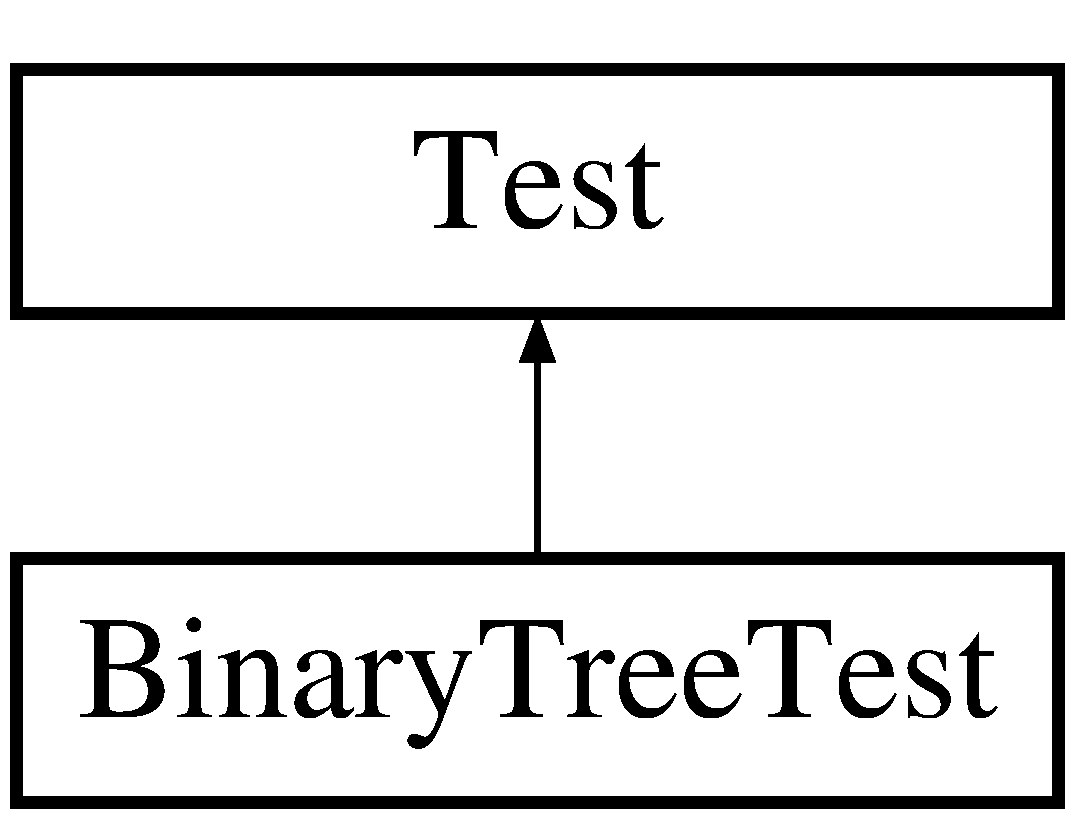
\includegraphics[height=2.000000cm]{class_binary_tree_test}
\end{center}
\end{figure}
\subsection*{Public Types}
\begin{DoxyCompactItemize}
\item 
typedef \hyperlink{struct_introduction_to_algorithm_1_1_tree_algorithm_1_1_binary_tree_node}{Binary\+Tree\+Node}$<$ int $>$ \hyperlink{class_binary_tree_test_ad4aa3d3d01bf0b1b820fffa58e81e15b}{Node}
\end{DoxyCompactItemize}
\subsection*{Protected Member Functions}
\begin{DoxyCompactItemize}
\item 
\hyperlink{class_binary_tree_test_ab650cb6b7b008479f5294b1ed65871e5}{Binary\+Tree\+Test} ()
\item 
void \hyperlink{class_binary_tree_test_ab718ba725e8099dda414f5dbc11e881b}{Set\+Up} ()
\begin{DoxyCompactList}\small\item\em Set\+Up\+:在每一个测试开始之前执行 \end{DoxyCompactList}\item 
void \hyperlink{class_binary_tree_test_ac8daf6a6b88e89733c0ade6da7d4a897}{Tear\+Down} ()
\begin{DoxyCompactList}\small\item\em Tear\+Down\+:在每一个测试结束之后执行 \end{DoxyCompactList}\end{DoxyCompactItemize}
\subsection*{Protected Attributes}
\begin{DoxyCompactItemize}
\item 
\hyperlink{struct_introduction_to_algorithm_1_1_tree_algorithm_1_1_binary_tree}{Binary\+Tree}$<$ \hyperlink{class_binary_tree_test_ad4aa3d3d01bf0b1b820fffa58e81e15b}{Node} $>$ \hyperlink{class_binary_tree_test_a66e48418e5449b663b2608f4914100d5}{\+\_\+empty\+\_\+tree}
\item 
\hyperlink{struct_introduction_to_algorithm_1_1_tree_algorithm_1_1_binary_tree}{Binary\+Tree}$<$ \hyperlink{class_binary_tree_test_ad4aa3d3d01bf0b1b820fffa58e81e15b}{Node} $>$ \hyperlink{class_binary_tree_test_a36a98db1094f92c94b7d7893c8975f57}{\+\_\+normal\+\_\+tree}
\end{DoxyCompactItemize}


\subsection{Detailed Description}
\hyperlink{class_binary_tree_test}{Binary\+Tree\+Test}\+:测试类,用于为测试提供基础数据 

{\ttfamily \hyperlink{class_binary_tree_test}{Binary\+Tree\+Test}}是 {\ttfamily \+::testing\+::\+Test} 的子类。它主要用于为每一个{\ttfamily T\+E\+S\+T\+\_\+\+F}准备测试环境 

Definition at line 37 of file binarytree\+\_\+test.\+h.



\subsection{Member Typedef Documentation}
\hypertarget{class_binary_tree_test_ad4aa3d3d01bf0b1b820fffa58e81e15b}{}\index{Binary\+Tree\+Test@{Binary\+Tree\+Test}!Node@{Node}}
\index{Node@{Node}!Binary\+Tree\+Test@{Binary\+Tree\+Test}}
\subsubsection[{Node}]{\setlength{\rightskip}{0pt plus 5cm}typedef {\bf Binary\+Tree\+Node}$<$int$>$ {\bf Binary\+Tree\+Test\+::\+Node}}\label{class_binary_tree_test_ad4aa3d3d01bf0b1b820fffa58e81e15b}


Definition at line 40 of file binarytree\+\_\+test.\+h.



\subsection{Constructor \& Destructor Documentation}
\hypertarget{class_binary_tree_test_ab650cb6b7b008479f5294b1ed65871e5}{}\index{Binary\+Tree\+Test@{Binary\+Tree\+Test}!Binary\+Tree\+Test@{Binary\+Tree\+Test}}
\index{Binary\+Tree\+Test@{Binary\+Tree\+Test}!Binary\+Tree\+Test@{Binary\+Tree\+Test}}
\subsubsection[{Binary\+Tree\+Test()}]{\setlength{\rightskip}{0pt plus 5cm}Binary\+Tree\+Test\+::\+Binary\+Tree\+Test (
\begin{DoxyParamCaption}
{}
\end{DoxyParamCaption}
)\hspace{0.3cm}{\ttfamily [inline]}, {\ttfamily [protected]}}\label{class_binary_tree_test_ab650cb6b7b008479f5294b1ed65871e5}


Definition at line 42 of file binarytree\+\_\+test.\+h.



\subsection{Member Function Documentation}
\hypertarget{class_binary_tree_test_ab718ba725e8099dda414f5dbc11e881b}{}\index{Binary\+Tree\+Test@{Binary\+Tree\+Test}!Set\+Up@{Set\+Up}}
\index{Set\+Up@{Set\+Up}!Binary\+Tree\+Test@{Binary\+Tree\+Test}}
\subsubsection[{Set\+Up()}]{\setlength{\rightskip}{0pt plus 5cm}void Binary\+Tree\+Test\+::\+Set\+Up (
\begin{DoxyParamCaption}
{}
\end{DoxyParamCaption}
)\hspace{0.3cm}{\ttfamily [inline]}, {\ttfamily [protected]}}\label{class_binary_tree_test_ab718ba725e8099dda414f5dbc11e881b}


Set\+Up\+:在每一个测试开始之前执行 

{\ttfamily Set\+Up}是 {\ttfamily \+::testing\+::\+Test} 的的虚函数。它主要用于为每一个测试提供测试环境 

Definition at line 49 of file binarytree\+\_\+test.\+h.

\hypertarget{class_binary_tree_test_ac8daf6a6b88e89733c0ade6da7d4a897}{}\index{Binary\+Tree\+Test@{Binary\+Tree\+Test}!Tear\+Down@{Tear\+Down}}
\index{Tear\+Down@{Tear\+Down}!Binary\+Tree\+Test@{Binary\+Tree\+Test}}
\subsubsection[{Tear\+Down()}]{\setlength{\rightskip}{0pt plus 5cm}void Binary\+Tree\+Test\+::\+Tear\+Down (
\begin{DoxyParamCaption}
{}
\end{DoxyParamCaption}
)\hspace{0.3cm}{\ttfamily [inline]}, {\ttfamily [protected]}}\label{class_binary_tree_test_ac8daf6a6b88e89733c0ade6da7d4a897}


Tear\+Down\+:在每一个测试结束之后执行 

{\ttfamily Tear\+Down}是 {\ttfamily \+::testing\+::\+Test} 的的虚函数。它主要用于为每个测试销毁测试环境 

Definition at line 89 of file binarytree\+\_\+test.\+h.



\subsection{Member Data Documentation}
\hypertarget{class_binary_tree_test_a66e48418e5449b663b2608f4914100d5}{}\index{Binary\+Tree\+Test@{Binary\+Tree\+Test}!\+\_\+empty\+\_\+tree@{\+\_\+empty\+\_\+tree}}
\index{\+\_\+empty\+\_\+tree@{\+\_\+empty\+\_\+tree}!Binary\+Tree\+Test@{Binary\+Tree\+Test}}
\subsubsection[{\+\_\+empty\+\_\+tree}]{\setlength{\rightskip}{0pt plus 5cm}{\bf Binary\+Tree}$<${\bf Node}$>$ Binary\+Tree\+Test\+::\+\_\+empty\+\_\+tree\hspace{0.3cm}{\ttfamily [protected]}}\label{class_binary_tree_test_a66e48418e5449b663b2608f4914100d5}
一个空的树 

Definition at line 91 of file binarytree\+\_\+test.\+h.

\hypertarget{class_binary_tree_test_a36a98db1094f92c94b7d7893c8975f57}{}\index{Binary\+Tree\+Test@{Binary\+Tree\+Test}!\+\_\+normal\+\_\+tree@{\+\_\+normal\+\_\+tree}}
\index{\+\_\+normal\+\_\+tree@{\+\_\+normal\+\_\+tree}!Binary\+Tree\+Test@{Binary\+Tree\+Test}}
\subsubsection[{\+\_\+normal\+\_\+tree}]{\setlength{\rightskip}{0pt plus 5cm}{\bf Binary\+Tree}$<${\bf Node}$>$ Binary\+Tree\+Test\+::\+\_\+normal\+\_\+tree\hspace{0.3cm}{\ttfamily [protected]}}\label{class_binary_tree_test_a36a98db1094f92c94b7d7893c8975f57}
一个非空的数 

Definition at line 92 of file binarytree\+\_\+test.\+h.



The documentation for this class was generated from the following file\+:\begin{DoxyCompactItemize}
\item 
src/tree\+\_\+algorithms/binarytree/\hyperlink{binarytree__test_8h}{binarytree\+\_\+test.\+h}\end{DoxyCompactItemize}

\hypertarget{class_connected_component_test}{}\section{Connected\+Component\+Test Class Reference}
\label{class_connected_component_test}\index{Connected\+Component\+Test@{Connected\+Component\+Test}}


\hyperlink{class_connected_component_test}{Connected\+Component\+Test}\+:测试类,用于为测试提供基础数据  




{\ttfamily \#include $<$connectedcomponent\+\_\+test.\+h$>$}

Inheritance diagram for Connected\+Component\+Test\+:\begin{figure}[H]
\begin{center}
\leavevmode
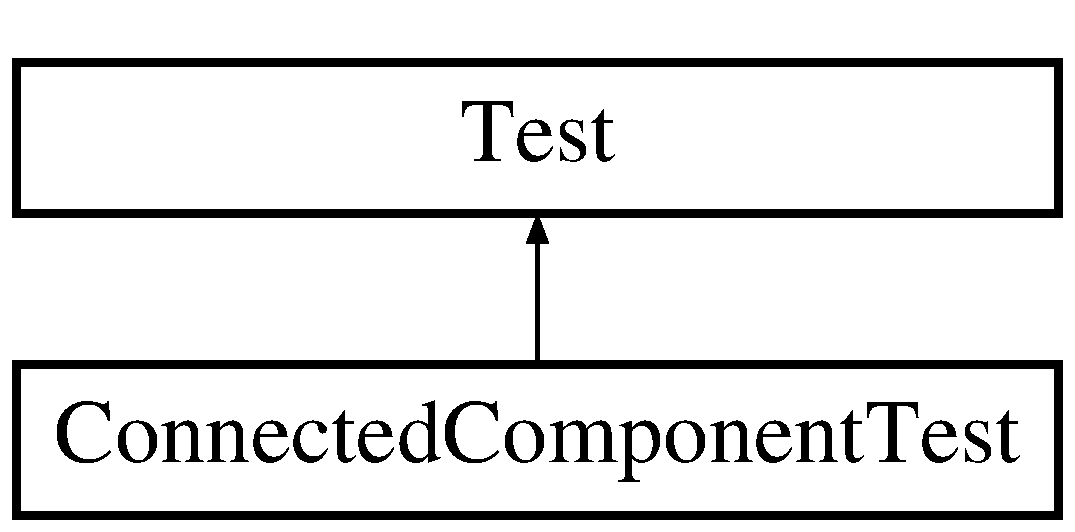
\includegraphics[height=2.000000cm]{class_connected_component_test}
\end{center}
\end{figure}
\subsection*{Public Types}
\begin{DoxyCompactItemize}
\item 
typedef \hyperlink{struct_introduction_to_algorithm_1_1_graph_algorithm_1_1_graph}{Graph}$<$ C\+\_\+\+N\+U\+M, \hyperlink{struct_introduction_to_algorithm_1_1_graph_algorithm_1_1_set_vertex}{Set\+Vertex}$<$ int $>$ $>$ \hyperlink{class_connected_component_test_a819b25542e9db5882ec64edb3bb78ff7}{G\+Type}
\end{DoxyCompactItemize}
\subsection*{Protected Member Functions}
\begin{DoxyCompactItemize}
\item 
void \hyperlink{class_connected_component_test_afd13b98fdaada57ea00e2bbde46144e2}{Set\+Up} ()
\item 
void \hyperlink{class_connected_component_test_a677db9fd4b9c973df7b78b402bf0a0f6}{Tear\+Down} ()
\end{DoxyCompactItemize}
\subsection*{Protected Attributes}
\begin{DoxyCompactItemize}
\item 
std\+::shared\+\_\+ptr$<$ \hyperlink{class_connected_component_test_a819b25542e9db5882ec64edb3bb78ff7}{G\+Type} $>$ \hyperlink{class_connected_component_test_a0f05d0ae37619e84f604aa51aa20cd28}{\+\_\+graph}
\end{DoxyCompactItemize}


\subsection{Detailed Description}
\hyperlink{class_connected_component_test}{Connected\+Component\+Test}\+:测试类,用于为测试提供基础数据 

{\ttfamily \hyperlink{class_connected_component_test}{Connected\+Component\+Test}}是 {\ttfamily \+::testing\+::\+Test} 的子类。它主要用于为每一个{\ttfamily T\+E\+S\+T\+\_\+\+F}准备测试环境 

Definition at line 40 of file connectedcomponent\+\_\+test.\+h.



\subsection{Member Typedef Documentation}
\hypertarget{class_connected_component_test_a819b25542e9db5882ec64edb3bb78ff7}{}\index{Connected\+Component\+Test@{Connected\+Component\+Test}!G\+Type@{G\+Type}}
\index{G\+Type@{G\+Type}!Connected\+Component\+Test@{Connected\+Component\+Test}}
\subsubsection[{G\+Type}]{\setlength{\rightskip}{0pt plus 5cm}typedef {\bf Graph}$<$C\+\_\+\+N\+U\+M,{\bf Set\+Vertex}$<$int$>$ $>$ {\bf Connected\+Component\+Test\+::\+G\+Type}}\label{class_connected_component_test_a819b25542e9db5882ec64edb3bb78ff7}
模板实例化的图类型,该图的顶点类型为{\ttfamily Set\+Vertex$<$int$>$} 

Definition at line 43 of file connectedcomponent\+\_\+test.\+h.



\subsection{Member Function Documentation}
\hypertarget{class_connected_component_test_afd13b98fdaada57ea00e2bbde46144e2}{}\index{Connected\+Component\+Test@{Connected\+Component\+Test}!Set\+Up@{Set\+Up}}
\index{Set\+Up@{Set\+Up}!Connected\+Component\+Test@{Connected\+Component\+Test}}
\subsubsection[{Set\+Up()}]{\setlength{\rightskip}{0pt plus 5cm}void Connected\+Component\+Test\+::\+Set\+Up (
\begin{DoxyParamCaption}
{}
\end{DoxyParamCaption}
)\hspace{0.3cm}{\ttfamily [inline]}, {\ttfamily [protected]}}\label{class_connected_component_test_afd13b98fdaada57ea00e2bbde46144e2}


Definition at line 45 of file connectedcomponent\+\_\+test.\+h.

\hypertarget{class_connected_component_test_a677db9fd4b9c973df7b78b402bf0a0f6}{}\index{Connected\+Component\+Test@{Connected\+Component\+Test}!Tear\+Down@{Tear\+Down}}
\index{Tear\+Down@{Tear\+Down}!Connected\+Component\+Test@{Connected\+Component\+Test}}
\subsubsection[{Tear\+Down()}]{\setlength{\rightskip}{0pt plus 5cm}void Connected\+Component\+Test\+::\+Tear\+Down (
\begin{DoxyParamCaption}
{}
\end{DoxyParamCaption}
)\hspace{0.3cm}{\ttfamily [inline]}, {\ttfamily [protected]}}\label{class_connected_component_test_a677db9fd4b9c973df7b78b402bf0a0f6}


Definition at line 58 of file connectedcomponent\+\_\+test.\+h.



\subsection{Member Data Documentation}
\hypertarget{class_connected_component_test_a0f05d0ae37619e84f604aa51aa20cd28}{}\index{Connected\+Component\+Test@{Connected\+Component\+Test}!\+\_\+graph@{\+\_\+graph}}
\index{\+\_\+graph@{\+\_\+graph}!Connected\+Component\+Test@{Connected\+Component\+Test}}
\subsubsection[{\+\_\+graph}]{\setlength{\rightskip}{0pt plus 5cm}std\+::shared\+\_\+ptr$<${\bf G\+Type}$>$ Connected\+Component\+Test\+::\+\_\+graph\hspace{0.3cm}{\ttfamily [protected]}}\label{class_connected_component_test_a0f05d0ae37619e84f604aa51aa20cd28}
测试连通分量的图的强指针 

Definition at line 60 of file connectedcomponent\+\_\+test.\+h.



The documentation for this class was generated from the following file\+:\begin{DoxyCompactItemize}
\item 
src/graph\+\_\+algorithms/basic\+\_\+graph/connected\+\_\+component/\hyperlink{connectedcomponent__test_8h}{connectedcomponent\+\_\+test.\+h}\end{DoxyCompactItemize}

\hypertarget{class_dag_shortest_path_test}{}\section{Dag\+Shortest\+Path\+Test Class Reference}
\label{class_dag_shortest_path_test}\index{Dag\+Shortest\+Path\+Test@{Dag\+Shortest\+Path\+Test}}


\hyperlink{class_dag_shortest_path_test}{Dag\+Shortest\+Path\+Test}\+:测试类,用于为测试提供基础数据  




{\ttfamily \#include $<$dagshortpath\+\_\+test.\+h$>$}

Inheritance diagram for Dag\+Shortest\+Path\+Test\+:\begin{figure}[H]
\begin{center}
\leavevmode
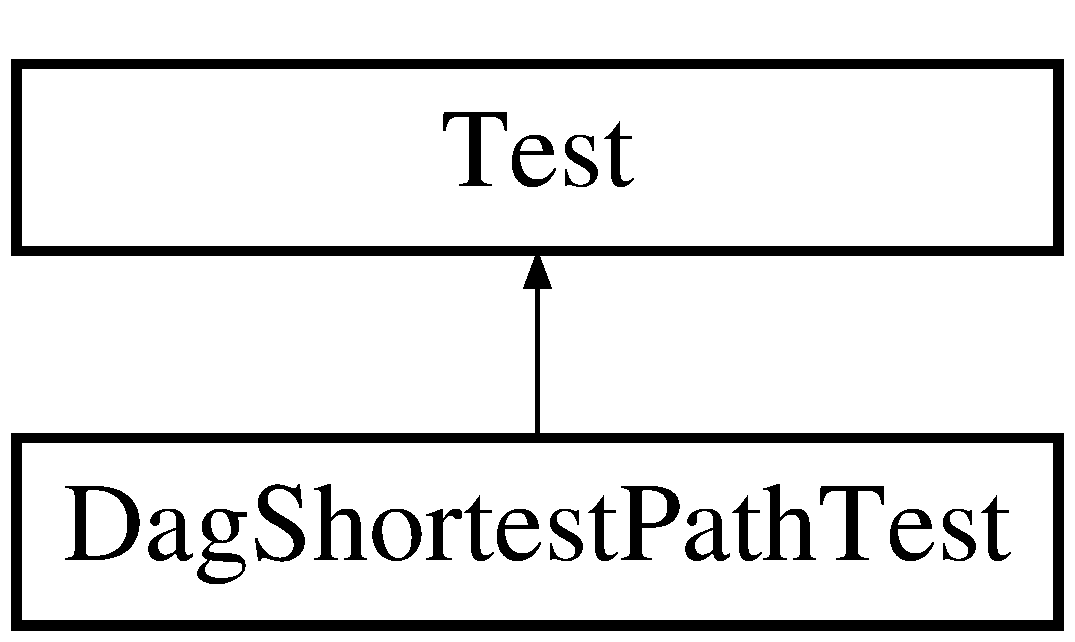
\includegraphics[height=2.000000cm]{class_dag_shortest_path_test}
\end{center}
\end{figure}
\subsection*{Public Types}
\begin{DoxyCompactItemize}
\item 
typedef \hyperlink{struct_introduction_to_algorithm_1_1_graph_algorithm_1_1_graph}{Graph}$<$ D\+S\+P\+\_\+\+N\+U\+M, \hyperlink{struct_introduction_to_algorithm_1_1_graph_algorithm_1_1_d_f_s___vertex}{D\+F\+S\+\_\+\+Vertex}$<$ int $>$ $>$ \hyperlink{class_dag_shortest_path_test_a55e732c7641684c040cf6a6a2a836efe}{G\+Type}
\item 
typedef \hyperlink{struct_introduction_to_algorithm_1_1_graph_algorithm_1_1_d_f_s___vertex}{D\+F\+S\+\_\+\+Vertex}$<$ int $>$ \hyperlink{class_dag_shortest_path_test_ad753154b61e842c086aff729e02b55ba}{Vertex\+Type}
\end{DoxyCompactItemize}
\subsection*{Protected Member Functions}
\begin{DoxyCompactItemize}
\item 
void \hyperlink{class_dag_shortest_path_test_a380ad10219669325d8c5e2ce8842a2ff}{Set\+Up} ()
\item 
void \hyperlink{class_dag_shortest_path_test_a8b59d67cc393896d103723fd6eaa6a96}{Tear\+Down} ()
\end{DoxyCompactItemize}
\subsection*{Protected Attributes}
\begin{DoxyCompactItemize}
\item 
std\+::shared\+\_\+ptr$<$ \hyperlink{class_dag_shortest_path_test_a55e732c7641684c040cf6a6a2a836efe}{G\+Type} $>$ \hyperlink{class_dag_shortest_path_test_a6d07675b5b9714443bdcb1d7da426624}{\+\_\+1v\+\_\+graph}
\item 
std\+::shared\+\_\+ptr$<$ \hyperlink{class_dag_shortest_path_test_a55e732c7641684c040cf6a6a2a836efe}{G\+Type} $>$ \hyperlink{class_dag_shortest_path_test_a63cb4f638b9be6c6f0647775fd2b3419}{\+\_\+1e\+\_\+graph}
\item 
std\+::shared\+\_\+ptr$<$ \hyperlink{class_dag_shortest_path_test_a55e732c7641684c040cf6a6a2a836efe}{G\+Type} $>$ \hyperlink{class_dag_shortest_path_test_ac96676722661c8d7ad6baf5bd4dbf3a7}{\+\_\+normal\+\_\+graph}
\end{DoxyCompactItemize}


\subsection{Detailed Description}
\hyperlink{class_dag_shortest_path_test}{Dag\+Shortest\+Path\+Test}\+:测试类,用于为测试提供基础数据 

{\ttfamily \hyperlink{class_dag_shortest_path_test}{Dag\+Shortest\+Path\+Test}}是 {\ttfamily \+::testing\+::\+Test} 的子类。它主要用于为每一个{\ttfamily T\+E\+S\+T\+\_\+\+F}准备测试环境 

Definition at line 39 of file dagshortpath\+\_\+test.\+h.



\subsection{Member Typedef Documentation}
\hypertarget{class_dag_shortest_path_test_a55e732c7641684c040cf6a6a2a836efe}{}\index{Dag\+Shortest\+Path\+Test@{Dag\+Shortest\+Path\+Test}!G\+Type@{G\+Type}}
\index{G\+Type@{G\+Type}!Dag\+Shortest\+Path\+Test@{Dag\+Shortest\+Path\+Test}}
\subsubsection[{G\+Type}]{\setlength{\rightskip}{0pt plus 5cm}typedef {\bf Graph}$<$D\+S\+P\+\_\+\+N\+U\+M,{\bf D\+F\+S\+\_\+\+Vertex}$<$int$>$ $>$ {\bf Dag\+Shortest\+Path\+Test\+::\+G\+Type}}\label{class_dag_shortest_path_test_a55e732c7641684c040cf6a6a2a836efe}
模板实例化的图类型,该图的顶点类型为{\ttfamily D\+F\+S\+\_\+\+Vertex$<$int$>$} 

Definition at line 42 of file dagshortpath\+\_\+test.\+h.

\hypertarget{class_dag_shortest_path_test_ad753154b61e842c086aff729e02b55ba}{}\index{Dag\+Shortest\+Path\+Test@{Dag\+Shortest\+Path\+Test}!Vertex\+Type@{Vertex\+Type}}
\index{Vertex\+Type@{Vertex\+Type}!Dag\+Shortest\+Path\+Test@{Dag\+Shortest\+Path\+Test}}
\subsubsection[{Vertex\+Type}]{\setlength{\rightskip}{0pt plus 5cm}typedef {\bf D\+F\+S\+\_\+\+Vertex}$<$int$>$ {\bf Dag\+Shortest\+Path\+Test\+::\+Vertex\+Type}}\label{class_dag_shortest_path_test_ad753154b61e842c086aff729e02b55ba}
图的顶点类型为{\ttfamily D\+F\+S\+\_\+\+Vertex$<$int$>$} 

Definition at line 43 of file dagshortpath\+\_\+test.\+h.



\subsection{Member Function Documentation}
\hypertarget{class_dag_shortest_path_test_a380ad10219669325d8c5e2ce8842a2ff}{}\index{Dag\+Shortest\+Path\+Test@{Dag\+Shortest\+Path\+Test}!Set\+Up@{Set\+Up}}
\index{Set\+Up@{Set\+Up}!Dag\+Shortest\+Path\+Test@{Dag\+Shortest\+Path\+Test}}
\subsubsection[{Set\+Up()}]{\setlength{\rightskip}{0pt plus 5cm}void Dag\+Shortest\+Path\+Test\+::\+Set\+Up (
\begin{DoxyParamCaption}
{}
\end{DoxyParamCaption}
)\hspace{0.3cm}{\ttfamily [inline]}, {\ttfamily [protected]}}\label{class_dag_shortest_path_test_a380ad10219669325d8c5e2ce8842a2ff}


Definition at line 45 of file dagshortpath\+\_\+test.\+h.

\hypertarget{class_dag_shortest_path_test_a8b59d67cc393896d103723fd6eaa6a96}{}\index{Dag\+Shortest\+Path\+Test@{Dag\+Shortest\+Path\+Test}!Tear\+Down@{Tear\+Down}}
\index{Tear\+Down@{Tear\+Down}!Dag\+Shortest\+Path\+Test@{Dag\+Shortest\+Path\+Test}}
\subsubsection[{Tear\+Down()}]{\setlength{\rightskip}{0pt plus 5cm}void Dag\+Shortest\+Path\+Test\+::\+Tear\+Down (
\begin{DoxyParamCaption}
{}
\end{DoxyParamCaption}
)\hspace{0.3cm}{\ttfamily [inline]}, {\ttfamily [protected]}}\label{class_dag_shortest_path_test_a8b59d67cc393896d103723fd6eaa6a96}


Definition at line 63 of file dagshortpath\+\_\+test.\+h.



\subsection{Member Data Documentation}
\hypertarget{class_dag_shortest_path_test_a63cb4f638b9be6c6f0647775fd2b3419}{}\index{Dag\+Shortest\+Path\+Test@{Dag\+Shortest\+Path\+Test}!\+\_\+1e\+\_\+graph@{\+\_\+1e\+\_\+graph}}
\index{\+\_\+1e\+\_\+graph@{\+\_\+1e\+\_\+graph}!Dag\+Shortest\+Path\+Test@{Dag\+Shortest\+Path\+Test}}
\subsubsection[{\+\_\+1e\+\_\+graph}]{\setlength{\rightskip}{0pt plus 5cm}std\+::shared\+\_\+ptr$<${\bf G\+Type}$>$ Dag\+Shortest\+Path\+Test\+::\+\_\+1e\+\_\+graph\hspace{0.3cm}{\ttfamily [protected]}}\label{class_dag_shortest_path_test_a63cb4f638b9be6c6f0647775fd2b3419}
指向一个图,该图只有一条边 

Definition at line 66 of file dagshortpath\+\_\+test.\+h.

\hypertarget{class_dag_shortest_path_test_a6d07675b5b9714443bdcb1d7da426624}{}\index{Dag\+Shortest\+Path\+Test@{Dag\+Shortest\+Path\+Test}!\+\_\+1v\+\_\+graph@{\+\_\+1v\+\_\+graph}}
\index{\+\_\+1v\+\_\+graph@{\+\_\+1v\+\_\+graph}!Dag\+Shortest\+Path\+Test@{Dag\+Shortest\+Path\+Test}}
\subsubsection[{\+\_\+1v\+\_\+graph}]{\setlength{\rightskip}{0pt plus 5cm}std\+::shared\+\_\+ptr$<${\bf G\+Type}$>$ Dag\+Shortest\+Path\+Test\+::\+\_\+1v\+\_\+graph\hspace{0.3cm}{\ttfamily [protected]}}\label{class_dag_shortest_path_test_a6d07675b5b9714443bdcb1d7da426624}
指向一个图,该图只有一个顶点 

Definition at line 65 of file dagshortpath\+\_\+test.\+h.

\hypertarget{class_dag_shortest_path_test_ac96676722661c8d7ad6baf5bd4dbf3a7}{}\index{Dag\+Shortest\+Path\+Test@{Dag\+Shortest\+Path\+Test}!\+\_\+normal\+\_\+graph@{\+\_\+normal\+\_\+graph}}
\index{\+\_\+normal\+\_\+graph@{\+\_\+normal\+\_\+graph}!Dag\+Shortest\+Path\+Test@{Dag\+Shortest\+Path\+Test}}
\subsubsection[{\+\_\+normal\+\_\+graph}]{\setlength{\rightskip}{0pt plus 5cm}std\+::shared\+\_\+ptr$<${\bf G\+Type}$>$ Dag\+Shortest\+Path\+Test\+::\+\_\+normal\+\_\+graph\hspace{0.3cm}{\ttfamily [protected]}}\label{class_dag_shortest_path_test_ac96676722661c8d7ad6baf5bd4dbf3a7}
指向一个图,该图的边组成一条链条 

Definition at line 67 of file dagshortpath\+\_\+test.\+h.



The documentation for this class was generated from the following file\+:\begin{DoxyCompactItemize}
\item 
src/graph\+\_\+algorithms/single\+\_\+source\+\_\+shortest\+\_\+path/dag\+\_\+shortest\+\_\+path/\hyperlink{dagshortpath__test_8h}{dagshortpath\+\_\+test.\+h}\end{DoxyCompactItemize}

\hypertarget{struct_introduction_to_algorithm_1_1_graph_algorithm_1_1_d_f_s___vertex}{}\section{Introduction\+To\+Algorithm\+:\+:Graph\+Algorithm\+:\+:D\+F\+S\+\_\+\+Vertex$<$ K\+Type $>$ Struct Template Reference}
\label{struct_introduction_to_algorithm_1_1_graph_algorithm_1_1_d_f_s___vertex}\index{Introduction\+To\+Algorithm\+::\+Graph\+Algorithm\+::\+D\+F\+S\+\_\+\+Vertex$<$ K\+Type $>$@{Introduction\+To\+Algorithm\+::\+Graph\+Algorithm\+::\+D\+F\+S\+\_\+\+Vertex$<$ K\+Type $>$}}


D\+F\+S\+\_\+\+Vertex:用于深度优先搜索的顶点类型,算法导论22章22.3节  




{\ttfamily \#include $<$dfs\+\_\+vertex.\+h$>$}

Inheritance diagram for Introduction\+To\+Algorithm\+:\+:Graph\+Algorithm\+:\+:D\+F\+S\+\_\+\+Vertex$<$ K\+Type $>$\+:\begin{figure}[H]
\begin{center}
\leavevmode
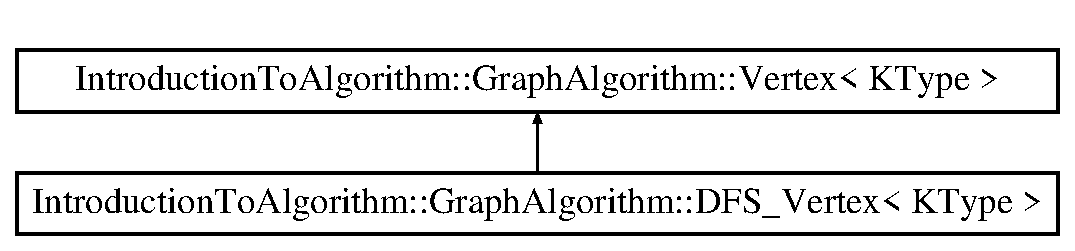
\includegraphics[height=2.000000cm]{struct_introduction_to_algorithm_1_1_graph_algorithm_1_1_d_f_s___vertex}
\end{center}
\end{figure}
\subsection*{Public Types}
\begin{DoxyCompactItemize}
\item 
enum \hyperlink{struct_introduction_to_algorithm_1_1_graph_algorithm_1_1_d_f_s___vertex_a9455444fdfb1b29f24c1d27e74e7c124}{C\+O\+L\+O\+R} \{ \hyperlink{struct_introduction_to_algorithm_1_1_graph_algorithm_1_1_d_f_s___vertex_a9455444fdfb1b29f24c1d27e74e7c124ab5bf627e448384cf3a4c35121ca6008d}{C\+O\+L\+O\+R\+::\+W\+H\+I\+T\+E}, 
\hyperlink{struct_introduction_to_algorithm_1_1_graph_algorithm_1_1_d_f_s___vertex_a9455444fdfb1b29f24c1d27e74e7c124a48bf014c704c9eaae100a98006a37bf7}{C\+O\+L\+O\+R\+::\+G\+R\+A\+Y}, 
\hyperlink{struct_introduction_to_algorithm_1_1_graph_algorithm_1_1_d_f_s___vertex_a9455444fdfb1b29f24c1d27e74e7c124a08d0012388564e95c3b4a7407cf04965}{C\+O\+L\+O\+R\+::\+B\+L\+A\+C\+K}
 \}
\item 
typedef int \hyperlink{struct_introduction_to_algorithm_1_1_graph_algorithm_1_1_d_f_s___vertex_aeb115a10366eb62880d2672d4e1da7a1}{V\+I\+D\+Type}
\item 
typedef K\+Type \hyperlink{struct_introduction_to_algorithm_1_1_graph_algorithm_1_1_d_f_s___vertex_ab53cda3a7d135ed892b298c14d5579fe}{Key\+Type}
\end{DoxyCompactItemize}
\subsection*{Public Member Functions}
\begin{DoxyCompactItemize}
\item 
\hyperlink{struct_introduction_to_algorithm_1_1_graph_algorithm_1_1_d_f_s___vertex_a91c4d3427c469cbb16459f6a34ac1307}{D\+F\+S\+\_\+\+Vertex} ()
\begin{DoxyCompactList}\small\item\em 默认构造函数,将{\ttfamily color}设为白色,发现时间与完成时间默认为-\/1 \end{DoxyCompactList}\item 
\hyperlink{struct_introduction_to_algorithm_1_1_graph_algorithm_1_1_d_f_s___vertex_a2b44ef3bada5ce96e84fbd5e6b8c0e56}{D\+F\+S\+\_\+\+Vertex} (const \hyperlink{struct_introduction_to_algorithm_1_1_graph_algorithm_1_1_d_f_s___vertex_ab53cda3a7d135ed892b298c14d5579fe}{Key\+Type} \&k)
\begin{DoxyCompactList}\small\item\em 显式构造函数,指定{\ttfamily key} \end{DoxyCompactList}\item 
\hyperlink{struct_introduction_to_algorithm_1_1_graph_algorithm_1_1_d_f_s___vertex_adbee712bffa03e88e3624a144528fe54}{D\+F\+S\+\_\+\+Vertex} (const \hyperlink{struct_introduction_to_algorithm_1_1_graph_algorithm_1_1_d_f_s___vertex_ab53cda3a7d135ed892b298c14d5579fe}{Key\+Type} \&k, \hyperlink{struct_introduction_to_algorithm_1_1_graph_algorithm_1_1_d_f_s___vertex_aeb115a10366eb62880d2672d4e1da7a1}{V\+I\+D\+Type} d)
\begin{DoxyCompactList}\small\item\em 显式构造函数,指定{\ttfamily key}和编号 \end{DoxyCompactList}\item 
void \hyperlink{struct_introduction_to_algorithm_1_1_graph_algorithm_1_1_d_f_s___vertex_ab1969489b2a5d73191da5664b127226d}{set\+\_\+disovered} (int discover\+\_\+t)
\begin{DoxyCompactList}\small\item\em set\+\_\+disovered:发现本顶点 \end{DoxyCompactList}\item 
void \hyperlink{struct_introduction_to_algorithm_1_1_graph_algorithm_1_1_d_f_s___vertex_a07353127c56aabb5c411ca7f4d28c553}{set\+\_\+finished} (int finish\+\_\+t)
\begin{DoxyCompactList}\small\item\em set\+\_\+finished:设本顶点为搜索完毕状态 \end{DoxyCompactList}\item 
std\+::string \hyperlink{struct_introduction_to_algorithm_1_1_graph_algorithm_1_1_d_f_s___vertex_a9a8a8c8b2ad1c3b6e90d2c2efb7cbe2e}{to\+\_\+string} ()
\begin{DoxyCompactList}\small\item\em to\+\_\+string:返回顶点的字符串描述 \end{DoxyCompactList}\end{DoxyCompactItemize}
\subsection*{Public Attributes}
\begin{DoxyCompactItemize}
\item 
int \hyperlink{struct_introduction_to_algorithm_1_1_graph_algorithm_1_1_d_f_s___vertex_aab1b292c1d228d57ef3d20af908fe2cf}{discover\+\_\+time}
\item 
int \hyperlink{struct_introduction_to_algorithm_1_1_graph_algorithm_1_1_d_f_s___vertex_aa0f17c70784c1dcc199487e519814e61}{finish\+\_\+time}
\item 
\hyperlink{struct_introduction_to_algorithm_1_1_graph_algorithm_1_1_d_f_s___vertex_a9455444fdfb1b29f24c1d27e74e7c124}{C\+O\+L\+O\+R} \hyperlink{struct_introduction_to_algorithm_1_1_graph_algorithm_1_1_d_f_s___vertex_a9111c3d35ad67867402564643493655f}{color}
\item 
std\+::shared\+\_\+ptr$<$ \hyperlink{struct_introduction_to_algorithm_1_1_graph_algorithm_1_1_d_f_s___vertex}{D\+F\+S\+\_\+\+Vertex} $>$ \hyperlink{struct_introduction_to_algorithm_1_1_graph_algorithm_1_1_d_f_s___vertex_ad243c81b3c0705a136b6a1e5debdb6ed}{parent}
\end{DoxyCompactItemize}


\subsection{Detailed Description}
\subsubsection*{template$<$typename K\+Type$>$struct Introduction\+To\+Algorithm\+::\+Graph\+Algorithm\+::\+D\+F\+S\+\_\+\+Vertex$<$ K\+Type $>$}

D\+F\+S\+\_\+\+Vertex:用于深度优先搜索的顶点类型,算法导论22章22.3节 

深度优先搜索的顶点类型继承自{\ttfamily \hyperlink{struct_introduction_to_algorithm_1_1_graph_algorithm_1_1_vertex}{Vertex}}模板类型,它比{\ttfamily \hyperlink{struct_introduction_to_algorithm_1_1_graph_algorithm_1_1_vertex}{Vertex}}多了四个数据成员:


\begin{DoxyItemize}
\item {\ttfamily color}:顶点的颜色。顶点可以有三种颜色,分别为{\ttfamily \hyperlink{struct_introduction_to_algorithm_1_1_graph_algorithm_1_1_d_f_s___vertex_a9455444fdfb1b29f24c1d27e74e7c124a08d0012388564e95c3b4a7407cf04965}{D\+F\+S\+\_\+\+Vertex\+::\+C\+O\+L\+O\+R\+::\+B\+L\+A\+C\+K}}、{\ttfamily \hyperlink{struct_introduction_to_algorithm_1_1_graph_algorithm_1_1_d_f_s___vertex_a9455444fdfb1b29f24c1d27e74e7c124ab5bf627e448384cf3a4c35121ca6008d}{D\+F\+S\+\_\+\+Vertex\+::\+C\+O\+L\+O\+R\+::\+W\+H\+I\+T\+E}}、{\ttfamily \hyperlink{struct_introduction_to_algorithm_1_1_graph_algorithm_1_1_d_f_s___vertex_a9455444fdfb1b29f24c1d27e74e7c124a48bf014c704c9eaae100a98006a37bf7}{D\+F\+S\+\_\+\+Vertex\+::\+C\+O\+L\+O\+R\+::\+G\+R\+A\+Y}}
\item {\ttfamily parent}\+: 指向父顶点的强引用
\item {\ttfamily discover\+\_\+time}:顶点的发现时间
\item {\ttfamily finish\+\_\+time}:顶点的完成时间
\end{DoxyItemize}

广度优先搜索的顶点类型还支持以下两个操作:


\begin{DoxyItemize}
\item {\ttfamily set\+\_\+disovered(discover\+\_\+t)}:发现本顶点
\item {\ttfamily set\+\_\+finished(finish\+\_\+t)}:本顶点搜索完毕 
\end{DoxyItemize}

Definition at line 42 of file dfs\+\_\+vertex.\+h.



\subsection{Member Typedef Documentation}
\hypertarget{struct_introduction_to_algorithm_1_1_graph_algorithm_1_1_d_f_s___vertex_ab53cda3a7d135ed892b298c14d5579fe}{}\index{Introduction\+To\+Algorithm\+::\+Graph\+Algorithm\+::\+D\+F\+S\+\_\+\+Vertex@{Introduction\+To\+Algorithm\+::\+Graph\+Algorithm\+::\+D\+F\+S\+\_\+\+Vertex}!Key\+Type@{Key\+Type}}
\index{Key\+Type@{Key\+Type}!Introduction\+To\+Algorithm\+::\+Graph\+Algorithm\+::\+D\+F\+S\+\_\+\+Vertex@{Introduction\+To\+Algorithm\+::\+Graph\+Algorithm\+::\+D\+F\+S\+\_\+\+Vertex}}
\subsubsection[{Key\+Type}]{\setlength{\rightskip}{0pt plus 5cm}template$<$typename K\+Type$>$ typedef K\+Type {\bf Introduction\+To\+Algorithm\+::\+Graph\+Algorithm\+::\+D\+F\+S\+\_\+\+Vertex}$<$ K\+Type $>$\+::{\bf Key\+Type}}\label{struct_introduction_to_algorithm_1_1_graph_algorithm_1_1_d_f_s___vertex_ab53cda3a7d135ed892b298c14d5579fe}
顶点存储数据的类型 

Definition at line 46 of file dfs\+\_\+vertex.\+h.

\hypertarget{struct_introduction_to_algorithm_1_1_graph_algorithm_1_1_d_f_s___vertex_aeb115a10366eb62880d2672d4e1da7a1}{}\index{Introduction\+To\+Algorithm\+::\+Graph\+Algorithm\+::\+D\+F\+S\+\_\+\+Vertex@{Introduction\+To\+Algorithm\+::\+Graph\+Algorithm\+::\+D\+F\+S\+\_\+\+Vertex}!V\+I\+D\+Type@{V\+I\+D\+Type}}
\index{V\+I\+D\+Type@{V\+I\+D\+Type}!Introduction\+To\+Algorithm\+::\+Graph\+Algorithm\+::\+D\+F\+S\+\_\+\+Vertex@{Introduction\+To\+Algorithm\+::\+Graph\+Algorithm\+::\+D\+F\+S\+\_\+\+Vertex}}
\subsubsection[{V\+I\+D\+Type}]{\setlength{\rightskip}{0pt plus 5cm}template$<$typename K\+Type$>$ typedef int {\bf Introduction\+To\+Algorithm\+::\+Graph\+Algorithm\+::\+D\+F\+S\+\_\+\+Vertex}$<$ K\+Type $>$\+::{\bf V\+I\+D\+Type}}\label{struct_introduction_to_algorithm_1_1_graph_algorithm_1_1_d_f_s___vertex_aeb115a10366eb62880d2672d4e1da7a1}
顶点编号的数据类型 

Definition at line 45 of file dfs\+\_\+vertex.\+h.



\subsection{Member Enumeration Documentation}
\hypertarget{struct_introduction_to_algorithm_1_1_graph_algorithm_1_1_d_f_s___vertex_a9455444fdfb1b29f24c1d27e74e7c124}{}\index{Introduction\+To\+Algorithm\+::\+Graph\+Algorithm\+::\+D\+F\+S\+\_\+\+Vertex@{Introduction\+To\+Algorithm\+::\+Graph\+Algorithm\+::\+D\+F\+S\+\_\+\+Vertex}!C\+O\+L\+O\+R@{C\+O\+L\+O\+R}}
\index{C\+O\+L\+O\+R@{C\+O\+L\+O\+R}!Introduction\+To\+Algorithm\+::\+Graph\+Algorithm\+::\+D\+F\+S\+\_\+\+Vertex@{Introduction\+To\+Algorithm\+::\+Graph\+Algorithm\+::\+D\+F\+S\+\_\+\+Vertex}}
\subsubsection[{C\+O\+L\+O\+R}]{\setlength{\rightskip}{0pt plus 5cm}template$<$typename K\+Type$>$ enum {\bf Introduction\+To\+Algorithm\+::\+Graph\+Algorithm\+::\+D\+F\+S\+\_\+\+Vertex\+::\+C\+O\+L\+O\+R}\hspace{0.3cm}{\ttfamily [strong]}}\label{struct_introduction_to_algorithm_1_1_graph_algorithm_1_1_d_f_s___vertex_a9455444fdfb1b29f24c1d27e74e7c124}
\begin{Desc}
\item[Enumerator]\par
\begin{description}
\index{W\+H\+I\+T\+E@{W\+H\+I\+T\+E}!Introduction\+To\+Algorithm\+::\+Graph\+Algorithm\+::\+D\+F\+S\+\_\+\+Vertex@{Introduction\+To\+Algorithm\+::\+Graph\+Algorithm\+::\+D\+F\+S\+\_\+\+Vertex}}\index{Introduction\+To\+Algorithm\+::\+Graph\+Algorithm\+::\+D\+F\+S\+\_\+\+Vertex@{Introduction\+To\+Algorithm\+::\+Graph\+Algorithm\+::\+D\+F\+S\+\_\+\+Vertex}!W\+H\+I\+T\+E@{W\+H\+I\+T\+E}}\item[{\em 
\hypertarget{struct_introduction_to_algorithm_1_1_graph_algorithm_1_1_d_f_s___vertex_a9455444fdfb1b29f24c1d27e74e7c124ab5bf627e448384cf3a4c35121ca6008d}{}W\+H\+I\+T\+E\label{struct_introduction_to_algorithm_1_1_graph_algorithm_1_1_d_f_s___vertex_a9455444fdfb1b29f24c1d27e74e7c124ab5bf627e448384cf3a4c35121ca6008d}
}]\index{G\+R\+A\+Y@{G\+R\+A\+Y}!Introduction\+To\+Algorithm\+::\+Graph\+Algorithm\+::\+D\+F\+S\+\_\+\+Vertex@{Introduction\+To\+Algorithm\+::\+Graph\+Algorithm\+::\+D\+F\+S\+\_\+\+Vertex}}\index{Introduction\+To\+Algorithm\+::\+Graph\+Algorithm\+::\+D\+F\+S\+\_\+\+Vertex@{Introduction\+To\+Algorithm\+::\+Graph\+Algorithm\+::\+D\+F\+S\+\_\+\+Vertex}!G\+R\+A\+Y@{G\+R\+A\+Y}}\item[{\em 
\hypertarget{struct_introduction_to_algorithm_1_1_graph_algorithm_1_1_d_f_s___vertex_a9455444fdfb1b29f24c1d27e74e7c124a48bf014c704c9eaae100a98006a37bf7}{}G\+R\+A\+Y\label{struct_introduction_to_algorithm_1_1_graph_algorithm_1_1_d_f_s___vertex_a9455444fdfb1b29f24c1d27e74e7c124a48bf014c704c9eaae100a98006a37bf7}
}]\index{B\+L\+A\+C\+K@{B\+L\+A\+C\+K}!Introduction\+To\+Algorithm\+::\+Graph\+Algorithm\+::\+D\+F\+S\+\_\+\+Vertex@{Introduction\+To\+Algorithm\+::\+Graph\+Algorithm\+::\+D\+F\+S\+\_\+\+Vertex}}\index{Introduction\+To\+Algorithm\+::\+Graph\+Algorithm\+::\+D\+F\+S\+\_\+\+Vertex@{Introduction\+To\+Algorithm\+::\+Graph\+Algorithm\+::\+D\+F\+S\+\_\+\+Vertex}!B\+L\+A\+C\+K@{B\+L\+A\+C\+K}}\item[{\em 
\hypertarget{struct_introduction_to_algorithm_1_1_graph_algorithm_1_1_d_f_s___vertex_a9455444fdfb1b29f24c1d27e74e7c124a08d0012388564e95c3b4a7407cf04965}{}B\+L\+A\+C\+K\label{struct_introduction_to_algorithm_1_1_graph_algorithm_1_1_d_f_s___vertex_a9455444fdfb1b29f24c1d27e74e7c124a08d0012388564e95c3b4a7407cf04965}
}]\end{description}
\end{Desc}


Definition at line 47 of file dfs\+\_\+vertex.\+h.



\subsection{Constructor \& Destructor Documentation}
\hypertarget{struct_introduction_to_algorithm_1_1_graph_algorithm_1_1_d_f_s___vertex_a91c4d3427c469cbb16459f6a34ac1307}{}\index{Introduction\+To\+Algorithm\+::\+Graph\+Algorithm\+::\+D\+F\+S\+\_\+\+Vertex@{Introduction\+To\+Algorithm\+::\+Graph\+Algorithm\+::\+D\+F\+S\+\_\+\+Vertex}!D\+F\+S\+\_\+\+Vertex@{D\+F\+S\+\_\+\+Vertex}}
\index{D\+F\+S\+\_\+\+Vertex@{D\+F\+S\+\_\+\+Vertex}!Introduction\+To\+Algorithm\+::\+Graph\+Algorithm\+::\+D\+F\+S\+\_\+\+Vertex@{Introduction\+To\+Algorithm\+::\+Graph\+Algorithm\+::\+D\+F\+S\+\_\+\+Vertex}}
\subsubsection[{D\+F\+S\+\_\+\+Vertex()}]{\setlength{\rightskip}{0pt plus 5cm}template$<$typename K\+Type$>$ {\bf Introduction\+To\+Algorithm\+::\+Graph\+Algorithm\+::\+D\+F\+S\+\_\+\+Vertex}$<$ K\+Type $>$\+::{\bf D\+F\+S\+\_\+\+Vertex} (
\begin{DoxyParamCaption}
{}
\end{DoxyParamCaption}
)\hspace{0.3cm}{\ttfamily [inline]}}\label{struct_introduction_to_algorithm_1_1_graph_algorithm_1_1_d_f_s___vertex_a91c4d3427c469cbb16459f6a34ac1307}


默认构造函数,将{\ttfamily color}设为白色,发现时间与完成时间默认为-\/1 



Definition at line 51 of file dfs\+\_\+vertex.\+h.

\hypertarget{struct_introduction_to_algorithm_1_1_graph_algorithm_1_1_d_f_s___vertex_a2b44ef3bada5ce96e84fbd5e6b8c0e56}{}\index{Introduction\+To\+Algorithm\+::\+Graph\+Algorithm\+::\+D\+F\+S\+\_\+\+Vertex@{Introduction\+To\+Algorithm\+::\+Graph\+Algorithm\+::\+D\+F\+S\+\_\+\+Vertex}!D\+F\+S\+\_\+\+Vertex@{D\+F\+S\+\_\+\+Vertex}}
\index{D\+F\+S\+\_\+\+Vertex@{D\+F\+S\+\_\+\+Vertex}!Introduction\+To\+Algorithm\+::\+Graph\+Algorithm\+::\+D\+F\+S\+\_\+\+Vertex@{Introduction\+To\+Algorithm\+::\+Graph\+Algorithm\+::\+D\+F\+S\+\_\+\+Vertex}}
\subsubsection[{D\+F\+S\+\_\+\+Vertex(const Key\+Type \&k)}]{\setlength{\rightskip}{0pt plus 5cm}template$<$typename K\+Type$>$ {\bf Introduction\+To\+Algorithm\+::\+Graph\+Algorithm\+::\+D\+F\+S\+\_\+\+Vertex}$<$ K\+Type $>$\+::{\bf D\+F\+S\+\_\+\+Vertex} (
\begin{DoxyParamCaption}
\item[{const {\bf Key\+Type} \&}]{k}
\end{DoxyParamCaption}
)\hspace{0.3cm}{\ttfamily [inline]}, {\ttfamily [explicit]}}\label{struct_introduction_to_algorithm_1_1_graph_algorithm_1_1_d_f_s___vertex_a2b44ef3bada5ce96e84fbd5e6b8c0e56}


显式构造函数,指定{\ttfamily key} 


\begin{DoxyParams}{Parameters}
{\em k\+:顶点存放的数据} & 顶点的颜色默认设为白色,发现时间与完成时间默认为-\/1 \\
\hline
\end{DoxyParams}


Definition at line 58 of file dfs\+\_\+vertex.\+h.

\hypertarget{struct_introduction_to_algorithm_1_1_graph_algorithm_1_1_d_f_s___vertex_adbee712bffa03e88e3624a144528fe54}{}\index{Introduction\+To\+Algorithm\+::\+Graph\+Algorithm\+::\+D\+F\+S\+\_\+\+Vertex@{Introduction\+To\+Algorithm\+::\+Graph\+Algorithm\+::\+D\+F\+S\+\_\+\+Vertex}!D\+F\+S\+\_\+\+Vertex@{D\+F\+S\+\_\+\+Vertex}}
\index{D\+F\+S\+\_\+\+Vertex@{D\+F\+S\+\_\+\+Vertex}!Introduction\+To\+Algorithm\+::\+Graph\+Algorithm\+::\+D\+F\+S\+\_\+\+Vertex@{Introduction\+To\+Algorithm\+::\+Graph\+Algorithm\+::\+D\+F\+S\+\_\+\+Vertex}}
\subsubsection[{D\+F\+S\+\_\+\+Vertex(const Key\+Type \&k, V\+I\+D\+Type d)}]{\setlength{\rightskip}{0pt plus 5cm}template$<$typename K\+Type$>$ {\bf Introduction\+To\+Algorithm\+::\+Graph\+Algorithm\+::\+D\+F\+S\+\_\+\+Vertex}$<$ K\+Type $>$\+::{\bf D\+F\+S\+\_\+\+Vertex} (
\begin{DoxyParamCaption}
\item[{const {\bf Key\+Type} \&}]{k, }
\item[{{\bf V\+I\+D\+Type}}]{d}
\end{DoxyParamCaption}
)\hspace{0.3cm}{\ttfamily [inline]}}\label{struct_introduction_to_algorithm_1_1_graph_algorithm_1_1_d_f_s___vertex_adbee712bffa03e88e3624a144528fe54}


显式构造函数,指定{\ttfamily key}和编号 


\begin{DoxyParams}{Parameters}
{\em k\+:顶点存放的数据} & \\
\hline
{\em d\+:顶点的编号} & 顶点的颜色默认设为白色,发现时间与完成时间默认为-\/1 \\
\hline
\end{DoxyParams}


Definition at line 68 of file dfs\+\_\+vertex.\+h.



\subsection{Member Function Documentation}
\hypertarget{struct_introduction_to_algorithm_1_1_graph_algorithm_1_1_d_f_s___vertex_ab1969489b2a5d73191da5664b127226d}{}\index{Introduction\+To\+Algorithm\+::\+Graph\+Algorithm\+::\+D\+F\+S\+\_\+\+Vertex@{Introduction\+To\+Algorithm\+::\+Graph\+Algorithm\+::\+D\+F\+S\+\_\+\+Vertex}!set\+\_\+disovered@{set\+\_\+disovered}}
\index{set\+\_\+disovered@{set\+\_\+disovered}!Introduction\+To\+Algorithm\+::\+Graph\+Algorithm\+::\+D\+F\+S\+\_\+\+Vertex@{Introduction\+To\+Algorithm\+::\+Graph\+Algorithm\+::\+D\+F\+S\+\_\+\+Vertex}}
\subsubsection[{set\+\_\+disovered(int discover\+\_\+t)}]{\setlength{\rightskip}{0pt plus 5cm}template$<$typename K\+Type$>$ void {\bf Introduction\+To\+Algorithm\+::\+Graph\+Algorithm\+::\+D\+F\+S\+\_\+\+Vertex}$<$ K\+Type $>$\+::set\+\_\+disovered (
\begin{DoxyParamCaption}
\item[{int}]{discover\+\_\+t}
\end{DoxyParamCaption}
)\hspace{0.3cm}{\ttfamily [inline]}}\label{struct_introduction_to_algorithm_1_1_graph_algorithm_1_1_d_f_s___vertex_ab1969489b2a5d73191da5664b127226d}


set\+\_\+disovered:发现本顶点 


\begin{DoxyParams}{Parameters}
{\em discover\+\_\+t\+:发现时间} & 发现本顶点要执行两个操作:\\
\hline
\end{DoxyParams}

\begin{DoxyItemize}
\item 将本顶点的颜色设为灰色
\item 将本顶点的{\ttfamily discover\+\_\+time}设为{\ttfamily discover\+\_\+t} 
\end{DoxyItemize}

Definition at line 81 of file dfs\+\_\+vertex.\+h.

\hypertarget{struct_introduction_to_algorithm_1_1_graph_algorithm_1_1_d_f_s___vertex_a07353127c56aabb5c411ca7f4d28c553}{}\index{Introduction\+To\+Algorithm\+::\+Graph\+Algorithm\+::\+D\+F\+S\+\_\+\+Vertex@{Introduction\+To\+Algorithm\+::\+Graph\+Algorithm\+::\+D\+F\+S\+\_\+\+Vertex}!set\+\_\+finished@{set\+\_\+finished}}
\index{set\+\_\+finished@{set\+\_\+finished}!Introduction\+To\+Algorithm\+::\+Graph\+Algorithm\+::\+D\+F\+S\+\_\+\+Vertex@{Introduction\+To\+Algorithm\+::\+Graph\+Algorithm\+::\+D\+F\+S\+\_\+\+Vertex}}
\subsubsection[{set\+\_\+finished(int finish\+\_\+t)}]{\setlength{\rightskip}{0pt plus 5cm}template$<$typename K\+Type$>$ void {\bf Introduction\+To\+Algorithm\+::\+Graph\+Algorithm\+::\+D\+F\+S\+\_\+\+Vertex}$<$ K\+Type $>$\+::set\+\_\+finished (
\begin{DoxyParamCaption}
\item[{int}]{finish\+\_\+t}
\end{DoxyParamCaption}
)\hspace{0.3cm}{\ttfamily [inline]}}\label{struct_introduction_to_algorithm_1_1_graph_algorithm_1_1_d_f_s___vertex_a07353127c56aabb5c411ca7f4d28c553}


set\+\_\+finished:设本顶点为搜索完毕状态 


\begin{DoxyParams}{Parameters}
{\em finish\+\_\+t\+:完成时间} & 设本顶点为搜索完毕状态要执行两个操作:\\
\hline
\end{DoxyParams}

\begin{DoxyItemize}
\item 将本顶点的颜色设为黑色
\item 将本顶点的{\ttfamily finish\+\_\+time}设为{\ttfamily finish\+\_\+t} 
\end{DoxyItemize}

Definition at line 96 of file dfs\+\_\+vertex.\+h.

\hypertarget{struct_introduction_to_algorithm_1_1_graph_algorithm_1_1_d_f_s___vertex_a9a8a8c8b2ad1c3b6e90d2c2efb7cbe2e}{}\index{Introduction\+To\+Algorithm\+::\+Graph\+Algorithm\+::\+D\+F\+S\+\_\+\+Vertex@{Introduction\+To\+Algorithm\+::\+Graph\+Algorithm\+::\+D\+F\+S\+\_\+\+Vertex}!to\+\_\+string@{to\+\_\+string}}
\index{to\+\_\+string@{to\+\_\+string}!Introduction\+To\+Algorithm\+::\+Graph\+Algorithm\+::\+D\+F\+S\+\_\+\+Vertex@{Introduction\+To\+Algorithm\+::\+Graph\+Algorithm\+::\+D\+F\+S\+\_\+\+Vertex}}
\subsubsection[{to\+\_\+string()}]{\setlength{\rightskip}{0pt plus 5cm}template$<$typename K\+Type$>$ std\+::string {\bf Introduction\+To\+Algorithm\+::\+Graph\+Algorithm\+::\+D\+F\+S\+\_\+\+Vertex}$<$ K\+Type $>$\+::to\+\_\+string (
\begin{DoxyParamCaption}
{}
\end{DoxyParamCaption}
)\hspace{0.3cm}{\ttfamily [inline]}}\label{struct_introduction_to_algorithm_1_1_graph_algorithm_1_1_d_f_s___vertex_a9a8a8c8b2ad1c3b6e90d2c2efb7cbe2e}


to\+\_\+string:返回顶点的字符串描述 

\begin{DoxyReturn}{Returns}
\+:顶点的字符串描述
\end{DoxyReturn}
在{\ttfamily \hyperlink{struct_introduction_to_algorithm_1_1_graph_algorithm_1_1_vertex}{Vertex}}基类的基础上输出{\ttfamily color}以及{\ttfamily parent}、{\ttfamily discover\+\_\+time}以及{\ttfamily finish\+\_\+time}信息。 

Definition at line 107 of file dfs\+\_\+vertex.\+h.



\subsection{Member Data Documentation}
\hypertarget{struct_introduction_to_algorithm_1_1_graph_algorithm_1_1_d_f_s___vertex_a9111c3d35ad67867402564643493655f}{}\index{Introduction\+To\+Algorithm\+::\+Graph\+Algorithm\+::\+D\+F\+S\+\_\+\+Vertex@{Introduction\+To\+Algorithm\+::\+Graph\+Algorithm\+::\+D\+F\+S\+\_\+\+Vertex}!color@{color}}
\index{color@{color}!Introduction\+To\+Algorithm\+::\+Graph\+Algorithm\+::\+D\+F\+S\+\_\+\+Vertex@{Introduction\+To\+Algorithm\+::\+Graph\+Algorithm\+::\+D\+F\+S\+\_\+\+Vertex}}
\subsubsection[{color}]{\setlength{\rightskip}{0pt plus 5cm}template$<$typename K\+Type$>$ {\bf C\+O\+L\+O\+R} {\bf Introduction\+To\+Algorithm\+::\+Graph\+Algorithm\+::\+D\+F\+S\+\_\+\+Vertex}$<$ K\+Type $>$\+::color}\label{struct_introduction_to_algorithm_1_1_graph_algorithm_1_1_d_f_s___vertex_a9111c3d35ad67867402564643493655f}
顶点颜色 

Definition at line 132 of file dfs\+\_\+vertex.\+h.

\hypertarget{struct_introduction_to_algorithm_1_1_graph_algorithm_1_1_d_f_s___vertex_aab1b292c1d228d57ef3d20af908fe2cf}{}\index{Introduction\+To\+Algorithm\+::\+Graph\+Algorithm\+::\+D\+F\+S\+\_\+\+Vertex@{Introduction\+To\+Algorithm\+::\+Graph\+Algorithm\+::\+D\+F\+S\+\_\+\+Vertex}!discover\+\_\+time@{discover\+\_\+time}}
\index{discover\+\_\+time@{discover\+\_\+time}!Introduction\+To\+Algorithm\+::\+Graph\+Algorithm\+::\+D\+F\+S\+\_\+\+Vertex@{Introduction\+To\+Algorithm\+::\+Graph\+Algorithm\+::\+D\+F\+S\+\_\+\+Vertex}}
\subsubsection[{discover\+\_\+time}]{\setlength{\rightskip}{0pt plus 5cm}template$<$typename K\+Type$>$ int {\bf Introduction\+To\+Algorithm\+::\+Graph\+Algorithm\+::\+D\+F\+S\+\_\+\+Vertex}$<$ K\+Type $>$\+::discover\+\_\+time}\label{struct_introduction_to_algorithm_1_1_graph_algorithm_1_1_d_f_s___vertex_aab1b292c1d228d57ef3d20af908fe2cf}
顶点发现时间 

Definition at line 130 of file dfs\+\_\+vertex.\+h.

\hypertarget{struct_introduction_to_algorithm_1_1_graph_algorithm_1_1_d_f_s___vertex_aa0f17c70784c1dcc199487e519814e61}{}\index{Introduction\+To\+Algorithm\+::\+Graph\+Algorithm\+::\+D\+F\+S\+\_\+\+Vertex@{Introduction\+To\+Algorithm\+::\+Graph\+Algorithm\+::\+D\+F\+S\+\_\+\+Vertex}!finish\+\_\+time@{finish\+\_\+time}}
\index{finish\+\_\+time@{finish\+\_\+time}!Introduction\+To\+Algorithm\+::\+Graph\+Algorithm\+::\+D\+F\+S\+\_\+\+Vertex@{Introduction\+To\+Algorithm\+::\+Graph\+Algorithm\+::\+D\+F\+S\+\_\+\+Vertex}}
\subsubsection[{finish\+\_\+time}]{\setlength{\rightskip}{0pt plus 5cm}template$<$typename K\+Type$>$ int {\bf Introduction\+To\+Algorithm\+::\+Graph\+Algorithm\+::\+D\+F\+S\+\_\+\+Vertex}$<$ K\+Type $>$\+::finish\+\_\+time}\label{struct_introduction_to_algorithm_1_1_graph_algorithm_1_1_d_f_s___vertex_aa0f17c70784c1dcc199487e519814e61}
顶点完成时间 

Definition at line 131 of file dfs\+\_\+vertex.\+h.

\hypertarget{struct_introduction_to_algorithm_1_1_graph_algorithm_1_1_d_f_s___vertex_ad243c81b3c0705a136b6a1e5debdb6ed}{}\index{Introduction\+To\+Algorithm\+::\+Graph\+Algorithm\+::\+D\+F\+S\+\_\+\+Vertex@{Introduction\+To\+Algorithm\+::\+Graph\+Algorithm\+::\+D\+F\+S\+\_\+\+Vertex}!parent@{parent}}
\index{parent@{parent}!Introduction\+To\+Algorithm\+::\+Graph\+Algorithm\+::\+D\+F\+S\+\_\+\+Vertex@{Introduction\+To\+Algorithm\+::\+Graph\+Algorithm\+::\+D\+F\+S\+\_\+\+Vertex}}
\subsubsection[{parent}]{\setlength{\rightskip}{0pt plus 5cm}template$<$typename K\+Type$>$ std\+::shared\+\_\+ptr$<${\bf D\+F\+S\+\_\+\+Vertex}$>$ {\bf Introduction\+To\+Algorithm\+::\+Graph\+Algorithm\+::\+D\+F\+S\+\_\+\+Vertex}$<$ K\+Type $>$\+::parent}\label{struct_introduction_to_algorithm_1_1_graph_algorithm_1_1_d_f_s___vertex_ad243c81b3c0705a136b6a1e5debdb6ed}
顶点父顶点的强引用 

Definition at line 133 of file dfs\+\_\+vertex.\+h.



The documentation for this struct was generated from the following file\+:\begin{DoxyCompactItemize}
\item 
src/graph\+\_\+algorithms/basic\+\_\+graph/graph\+\_\+representation/graph\+\_\+vertex/\hyperlink{dfs__vertex_8h}{dfs\+\_\+vertex.\+h}\end{DoxyCompactItemize}

\hypertarget{class_d_f_s_test}{}\section{D\+F\+S\+Test Class Reference}
\label{class_d_f_s_test}\index{D\+F\+S\+Test@{D\+F\+S\+Test}}


\hyperlink{class_d_f_s_test}{D\+F\+S\+Test}\+:测试类,用于为测试提供基础数据  




{\ttfamily \#include $<$dfs\+\_\+test.\+h$>$}

Inheritance diagram for D\+F\+S\+Test\+:\begin{figure}[H]
\begin{center}
\leavevmode
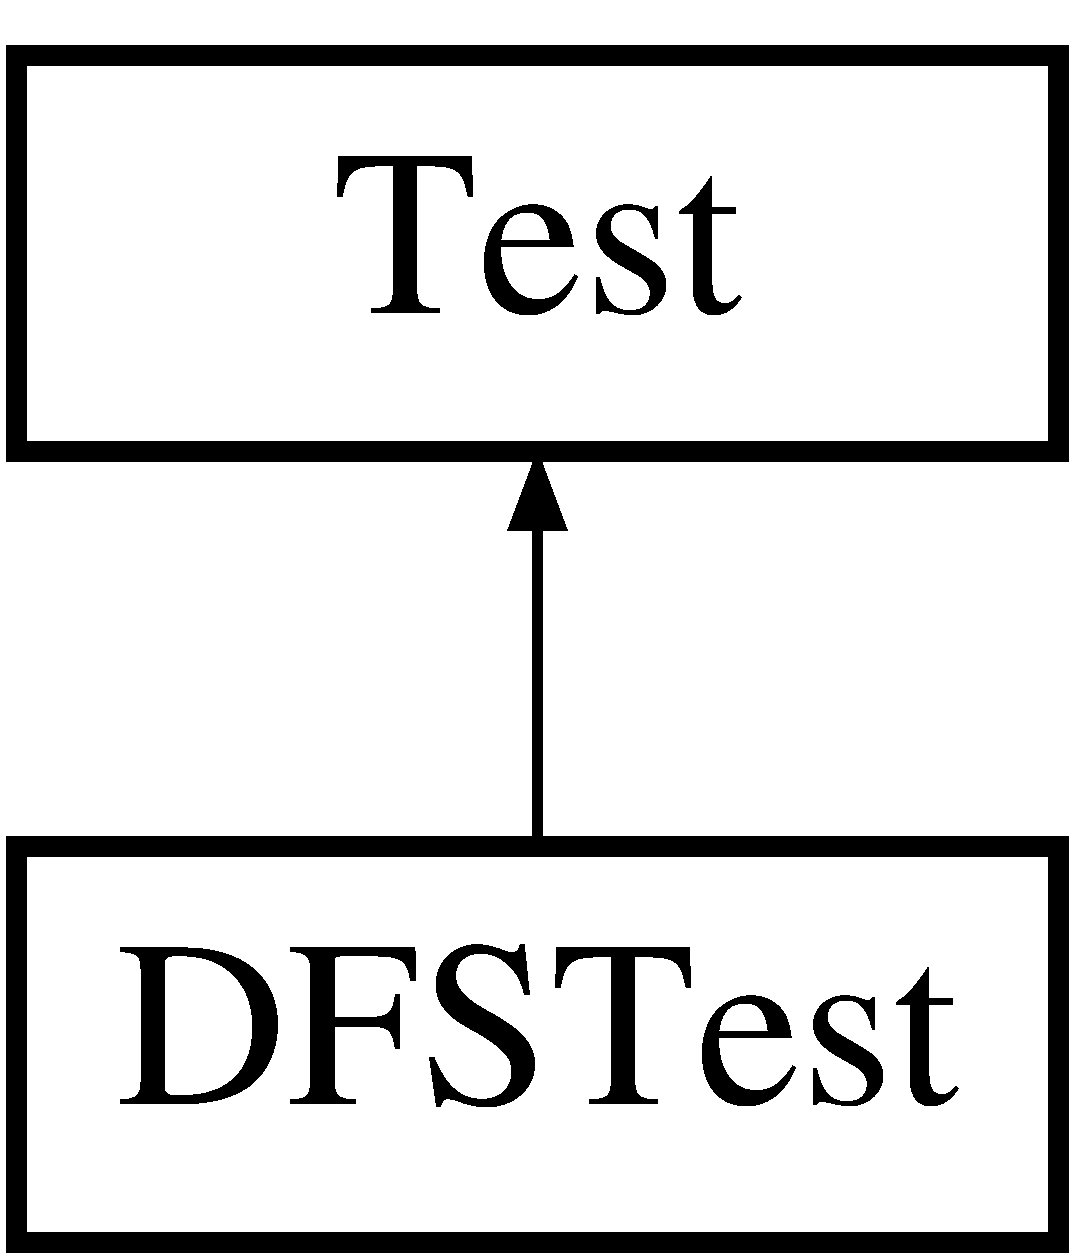
\includegraphics[height=2.000000cm]{class_d_f_s_test}
\end{center}
\end{figure}
\subsection*{Public Types}
\begin{DoxyCompactItemize}
\item 
typedef \hyperlink{struct_introduction_to_algorithm_1_1_graph_algorithm_1_1_graph}{Graph}$<$ D\+F\+S\+\_\+\+N, \hyperlink{struct_introduction_to_algorithm_1_1_graph_algorithm_1_1_d_f_s___vertex}{D\+F\+S\+\_\+\+Vertex}$<$ double $>$ $>$ \hyperlink{class_d_f_s_test_a32b63a9c79f6f7e7021daacf076a1512}{G\+Type}
\item 
typedef std\+::function$<$ void(\hyperlink{struct_introduction_to_algorithm_1_1_graph_algorithm_1_1_d_f_s___vertex}{D\+F\+S\+\_\+\+Vertex}$<$ double $>$\+::V\+I\+D\+Type v\+\_\+id, int time)$>$ \hyperlink{class_d_f_s_test_ac4c131b9b4f9de55192b1c634dc1c37f}{Action\+Type}
\end{DoxyCompactItemize}
\subsection*{Protected Member Functions}
\begin{DoxyCompactItemize}
\item 
void \hyperlink{class_d_f_s_test_aa8af56e0d079eb7c2b0ba7b6535d7d61}{Set\+Up} ()
\item 
void \hyperlink{class_d_f_s_test_afbe32ab6557cbca62368b480e1df593a}{Tear\+Down} ()
\end{DoxyCompactItemize}
\subsection*{Protected Attributes}
\begin{DoxyCompactItemize}
\item 
std\+::shared\+\_\+ptr$<$ \hyperlink{class_d_f_s_test_a32b63a9c79f6f7e7021daacf076a1512}{G\+Type} $>$ \hyperlink{class_d_f_s_test_a4dbae7784992bee522457b53da2141c2}{\+\_\+1v\+\_\+graph}
\item 
std\+::shared\+\_\+ptr$<$ \hyperlink{class_d_f_s_test_a32b63a9c79f6f7e7021daacf076a1512}{G\+Type} $>$ \hyperlink{class_d_f_s_test_ae5351e523345888ffc64aa892d93d3c2}{\+\_\+1e\+\_\+graph}
\item 
std\+::shared\+\_\+ptr$<$ \hyperlink{class_d_f_s_test_a32b63a9c79f6f7e7021daacf076a1512}{G\+Type} $>$ \hyperlink{class_d_f_s_test_a9607eac5350c4cdd449c353fed482efc}{\+\_\+list\+\_\+graph}
\item 
std\+::shared\+\_\+ptr$<$ \hyperlink{class_d_f_s_test_a32b63a9c79f6f7e7021daacf076a1512}{G\+Type} $>$ \hyperlink{class_d_f_s_test_a93a79d0654eb82517990c8f5419148a8}{\+\_\+rlist\+\_\+graph}
\end{DoxyCompactItemize}


\subsection{Detailed Description}
\hyperlink{class_d_f_s_test}{D\+F\+S\+Test}\+:测试类,用于为测试提供基础数据 

{\ttfamily \hyperlink{class_d_f_s_test}{D\+F\+S\+Test}}是 {\ttfamily \+::testing\+::\+Test} 的子类。它主要用于为每一个{\ttfamily T\+E\+S\+T\+\_\+\+F}准备测试环境 

Definition at line 42 of file dfs\+\_\+test.\+h.



\subsection{Member Typedef Documentation}
\hypertarget{class_d_f_s_test_ac4c131b9b4f9de55192b1c634dc1c37f}{}\index{D\+F\+S\+Test@{D\+F\+S\+Test}!Action\+Type@{Action\+Type}}
\index{Action\+Type@{Action\+Type}!D\+F\+S\+Test@{D\+F\+S\+Test}}
\subsubsection[{Action\+Type}]{\setlength{\rightskip}{0pt plus 5cm}typedef std\+::function$<$void({\bf D\+F\+S\+\_\+\+Vertex}$<$double$>$\+::V\+I\+D\+Type v\+\_\+id,int time)$>$ {\bf D\+F\+S\+Test\+::\+Action\+Type}}\label{class_d_f_s_test_ac4c131b9b4f9de55192b1c634dc1c37f}
模板实例化的\+Action类型 

Definition at line 46 of file dfs\+\_\+test.\+h.

\hypertarget{class_d_f_s_test_a32b63a9c79f6f7e7021daacf076a1512}{}\index{D\+F\+S\+Test@{D\+F\+S\+Test}!G\+Type@{G\+Type}}
\index{G\+Type@{G\+Type}!D\+F\+S\+Test@{D\+F\+S\+Test}}
\subsubsection[{G\+Type}]{\setlength{\rightskip}{0pt plus 5cm}typedef {\bf Graph}$<$D\+F\+S\+\_\+\+N,{\bf D\+F\+S\+\_\+\+Vertex}$<$double$>$ $>$ {\bf D\+F\+S\+Test\+::\+G\+Type}}\label{class_d_f_s_test_a32b63a9c79f6f7e7021daacf076a1512}
模板实例化的图类型,该图的顶点类型为{\ttfamily D\+F\+S\+\_\+\+Vertex$<$double$>$} 

Definition at line 45 of file dfs\+\_\+test.\+h.



\subsection{Member Function Documentation}
\hypertarget{class_d_f_s_test_aa8af56e0d079eb7c2b0ba7b6535d7d61}{}\index{D\+F\+S\+Test@{D\+F\+S\+Test}!Set\+Up@{Set\+Up}}
\index{Set\+Up@{Set\+Up}!D\+F\+S\+Test@{D\+F\+S\+Test}}
\subsubsection[{Set\+Up()}]{\setlength{\rightskip}{0pt plus 5cm}void D\+F\+S\+Test\+::\+Set\+Up (
\begin{DoxyParamCaption}
{}
\end{DoxyParamCaption}
)\hspace{0.3cm}{\ttfamily [inline]}, {\ttfamily [protected]}}\label{class_d_f_s_test_aa8af56e0d079eb7c2b0ba7b6535d7d61}


Definition at line 48 of file dfs\+\_\+test.\+h.

\hypertarget{class_d_f_s_test_afbe32ab6557cbca62368b480e1df593a}{}\index{D\+F\+S\+Test@{D\+F\+S\+Test}!Tear\+Down@{Tear\+Down}}
\index{Tear\+Down@{Tear\+Down}!D\+F\+S\+Test@{D\+F\+S\+Test}}
\subsubsection[{Tear\+Down()}]{\setlength{\rightskip}{0pt plus 5cm}void D\+F\+S\+Test\+::\+Tear\+Down (
\begin{DoxyParamCaption}
{}
\end{DoxyParamCaption}
)\hspace{0.3cm}{\ttfamily [inline]}, {\ttfamily [protected]}}\label{class_d_f_s_test_afbe32ab6557cbca62368b480e1df593a}


Definition at line 73 of file dfs\+\_\+test.\+h.



\subsection{Member Data Documentation}
\hypertarget{class_d_f_s_test_ae5351e523345888ffc64aa892d93d3c2}{}\index{D\+F\+S\+Test@{D\+F\+S\+Test}!\+\_\+1e\+\_\+graph@{\+\_\+1e\+\_\+graph}}
\index{\+\_\+1e\+\_\+graph@{\+\_\+1e\+\_\+graph}!D\+F\+S\+Test@{D\+F\+S\+Test}}
\subsubsection[{\+\_\+1e\+\_\+graph}]{\setlength{\rightskip}{0pt plus 5cm}std\+::shared\+\_\+ptr$<${\bf G\+Type}$>$ D\+F\+S\+Test\+::\+\_\+1e\+\_\+graph\hspace{0.3cm}{\ttfamily [protected]}}\label{class_d_f_s_test_ae5351e523345888ffc64aa892d93d3c2}
指向一个图,该图只有一条边 

Definition at line 75 of file dfs\+\_\+test.\+h.

\hypertarget{class_d_f_s_test_a4dbae7784992bee522457b53da2141c2}{}\index{D\+F\+S\+Test@{D\+F\+S\+Test}!\+\_\+1v\+\_\+graph@{\+\_\+1v\+\_\+graph}}
\index{\+\_\+1v\+\_\+graph@{\+\_\+1v\+\_\+graph}!D\+F\+S\+Test@{D\+F\+S\+Test}}
\subsubsection[{\+\_\+1v\+\_\+graph}]{\setlength{\rightskip}{0pt plus 5cm}std\+::shared\+\_\+ptr$<${\bf G\+Type}$>$ D\+F\+S\+Test\+::\+\_\+1v\+\_\+graph\hspace{0.3cm}{\ttfamily [protected]}}\label{class_d_f_s_test_a4dbae7784992bee522457b53da2141c2}
指向一个图,该图只有一个顶点 

Definition at line 74 of file dfs\+\_\+test.\+h.

\hypertarget{class_d_f_s_test_a9607eac5350c4cdd449c353fed482efc}{}\index{D\+F\+S\+Test@{D\+F\+S\+Test}!\+\_\+list\+\_\+graph@{\+\_\+list\+\_\+graph}}
\index{\+\_\+list\+\_\+graph@{\+\_\+list\+\_\+graph}!D\+F\+S\+Test@{D\+F\+S\+Test}}
\subsubsection[{\+\_\+list\+\_\+graph}]{\setlength{\rightskip}{0pt plus 5cm}std\+::shared\+\_\+ptr$<${\bf G\+Type}$>$ D\+F\+S\+Test\+::\+\_\+list\+\_\+graph\hspace{0.3cm}{\ttfamily [protected]}}\label{class_d_f_s_test_a9607eac5350c4cdd449c353fed482efc}
指向一个图,该图的边组成一个链条,该图用顺序搜索 

Definition at line 76 of file dfs\+\_\+test.\+h.

\hypertarget{class_d_f_s_test_a93a79d0654eb82517990c8f5419148a8}{}\index{D\+F\+S\+Test@{D\+F\+S\+Test}!\+\_\+rlist\+\_\+graph@{\+\_\+rlist\+\_\+graph}}
\index{\+\_\+rlist\+\_\+graph@{\+\_\+rlist\+\_\+graph}!D\+F\+S\+Test@{D\+F\+S\+Test}}
\subsubsection[{\+\_\+rlist\+\_\+graph}]{\setlength{\rightskip}{0pt plus 5cm}std\+::shared\+\_\+ptr$<${\bf G\+Type}$>$ D\+F\+S\+Test\+::\+\_\+rlist\+\_\+graph\hspace{0.3cm}{\ttfamily [protected]}}\label{class_d_f_s_test_a93a79d0654eb82517990c8f5419148a8}
指向一个图,该图的边组成一个链条,该图用逆序搜索 

Definition at line 77 of file dfs\+\_\+test.\+h.



The documentation for this class was generated from the following file\+:\begin{DoxyCompactItemize}
\item 
src/graph\+\_\+algorithms/basic\+\_\+graph/graph\+\_\+dfs/\hyperlink{dfs__test_8h}{dfs\+\_\+test.\+h}\end{DoxyCompactItemize}

\hypertarget{class_d_f_s_vertex_test}{}\section{D\+F\+S\+Vertex\+Test Class Reference}
\label{class_d_f_s_vertex_test}\index{D\+F\+S\+Vertex\+Test@{D\+F\+S\+Vertex\+Test}}


\hyperlink{class_d_f_s_vertex_test}{D\+F\+S\+Vertex\+Test}\+:测试类,用于为测试提供基础数据  




{\ttfamily \#include $<$dfs\+\_\+vertex\+\_\+test.\+h$>$}

Inheritance diagram for D\+F\+S\+Vertex\+Test\+:\begin{figure}[H]
\begin{center}
\leavevmode
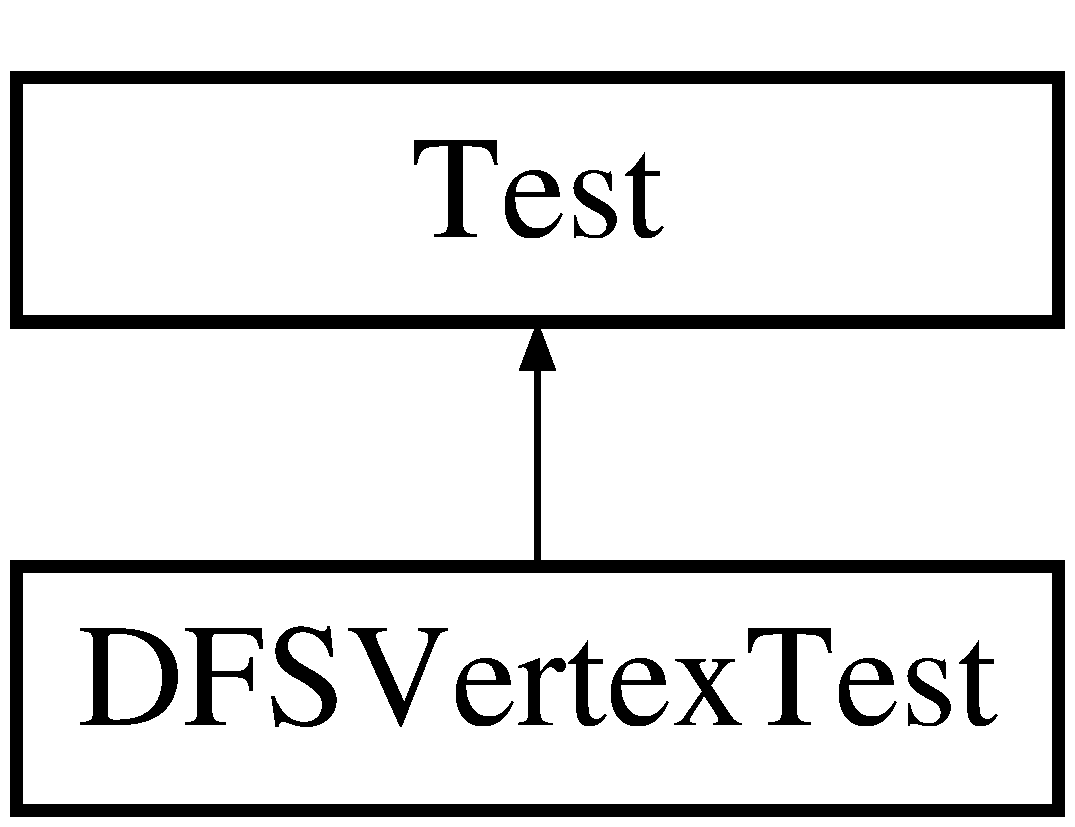
\includegraphics[height=2.000000cm]{class_d_f_s_vertex_test}
\end{center}
\end{figure}
\subsection*{Public Types}
\begin{DoxyCompactItemize}
\item 
typedef \hyperlink{class_d_f_s_vertex_test_aee693bcc01455e6f663b1404ce66e914}{D\+F\+S\+\_\+\+Vertex}$<$ double $>$ \hyperlink{class_d_f_s_vertex_test_aee693bcc01455e6f663b1404ce66e914}{D\+F\+S\+\_\+\+Vertex}
\end{DoxyCompactItemize}
\subsection*{Protected Member Functions}
\begin{DoxyCompactItemize}
\item 
void \hyperlink{class_d_f_s_vertex_test_a2a285e5c1ce500544b5591107e251357}{Set\+Up} ()
\item 
void \hyperlink{class_d_f_s_vertex_test_a3592b0e27fb73147848d2251eb063730}{Tear\+Down} ()
\end{DoxyCompactItemize}
\subsection*{Protected Attributes}
\begin{DoxyCompactItemize}
\item 
std\+::shared\+\_\+ptr$<$ \hyperlink{class_d_f_s_vertex_test_aee693bcc01455e6f663b1404ce66e914}{D\+F\+S\+\_\+\+Vertex} $>$ \hyperlink{class_d_f_s_vertex_test_aeb4886b7d27389066e8ade9c7d5a1b87}{\+\_\+default\+\_\+vertex}
\item 
std\+::shared\+\_\+ptr$<$ \hyperlink{class_d_f_s_vertex_test_aee693bcc01455e6f663b1404ce66e914}{D\+F\+S\+\_\+\+Vertex} $>$ \hyperlink{class_d_f_s_vertex_test_a7c88bbdb6487f913f67ed34f915381e4}{\+\_\+normal\+\_\+vertex}
\end{DoxyCompactItemize}


\subsection{Detailed Description}
\hyperlink{class_d_f_s_vertex_test}{D\+F\+S\+Vertex\+Test}\+:测试类,用于为测试提供基础数据 

{\ttfamily \hyperlink{class_d_f_s_vertex_test}{D\+F\+S\+Vertex\+Test}}是 {\ttfamily \+::testing\+::\+Test} 的子类。它主要用于为每一个{\ttfamily T\+E\+S\+T\+\_\+\+F}准备测试环境 

Definition at line 30 of file dfs\+\_\+vertex\+\_\+test.\+h.



\subsection{Member Typedef Documentation}
\hypertarget{class_d_f_s_vertex_test_aee693bcc01455e6f663b1404ce66e914}{}\index{D\+F\+S\+Vertex\+Test@{D\+F\+S\+Vertex\+Test}!D\+F\+S\+\_\+\+Vertex@{D\+F\+S\+\_\+\+Vertex}}
\index{D\+F\+S\+\_\+\+Vertex@{D\+F\+S\+\_\+\+Vertex}!D\+F\+S\+Vertex\+Test@{D\+F\+S\+Vertex\+Test}}
\subsubsection[{D\+F\+S\+\_\+\+Vertex}]{\setlength{\rightskip}{0pt plus 5cm}typedef {\bf D\+F\+S\+\_\+\+Vertex}$<$double$>$ {\bf D\+F\+S\+Vertex\+Test\+::\+D\+F\+S\+\_\+\+Vertex}}\label{class_d_f_s_vertex_test_aee693bcc01455e6f663b1404ce66e914}
模板实例化的顶点类型为{\ttfamily D\+F\+S\+\_\+\+Vertex$<$double$>$} 

Definition at line 33 of file dfs\+\_\+vertex\+\_\+test.\+h.



\subsection{Member Function Documentation}
\hypertarget{class_d_f_s_vertex_test_a2a285e5c1ce500544b5591107e251357}{}\index{D\+F\+S\+Vertex\+Test@{D\+F\+S\+Vertex\+Test}!Set\+Up@{Set\+Up}}
\index{Set\+Up@{Set\+Up}!D\+F\+S\+Vertex\+Test@{D\+F\+S\+Vertex\+Test}}
\subsubsection[{Set\+Up()}]{\setlength{\rightskip}{0pt plus 5cm}void D\+F\+S\+Vertex\+Test\+::\+Set\+Up (
\begin{DoxyParamCaption}
{}
\end{DoxyParamCaption}
)\hspace{0.3cm}{\ttfamily [inline]}, {\ttfamily [protected]}}\label{class_d_f_s_vertex_test_a2a285e5c1ce500544b5591107e251357}


Definition at line 36 of file dfs\+\_\+vertex\+\_\+test.\+h.

\hypertarget{class_d_f_s_vertex_test_a3592b0e27fb73147848d2251eb063730}{}\index{D\+F\+S\+Vertex\+Test@{D\+F\+S\+Vertex\+Test}!Tear\+Down@{Tear\+Down}}
\index{Tear\+Down@{Tear\+Down}!D\+F\+S\+Vertex\+Test@{D\+F\+S\+Vertex\+Test}}
\subsubsection[{Tear\+Down()}]{\setlength{\rightskip}{0pt plus 5cm}void D\+F\+S\+Vertex\+Test\+::\+Tear\+Down (
\begin{DoxyParamCaption}
{}
\end{DoxyParamCaption}
)\hspace{0.3cm}{\ttfamily [inline]}, {\ttfamily [protected]}}\label{class_d_f_s_vertex_test_a3592b0e27fb73147848d2251eb063730}


Definition at line 41 of file dfs\+\_\+vertex\+\_\+test.\+h.



\subsection{Member Data Documentation}
\hypertarget{class_d_f_s_vertex_test_aeb4886b7d27389066e8ade9c7d5a1b87}{}\index{D\+F\+S\+Vertex\+Test@{D\+F\+S\+Vertex\+Test}!\+\_\+default\+\_\+vertex@{\+\_\+default\+\_\+vertex}}
\index{\+\_\+default\+\_\+vertex@{\+\_\+default\+\_\+vertex}!D\+F\+S\+Vertex\+Test@{D\+F\+S\+Vertex\+Test}}
\subsubsection[{\+\_\+default\+\_\+vertex}]{\setlength{\rightskip}{0pt plus 5cm}std\+::shared\+\_\+ptr$<${\bf D\+F\+S\+\_\+\+Vertex}$>$ D\+F\+S\+Vertex\+Test\+::\+\_\+default\+\_\+vertex\hspace{0.3cm}{\ttfamily [protected]}}\label{class_d_f_s_vertex_test_aeb4886b7d27389066e8ade9c7d5a1b87}
指向一个默认构造的顶点 

Definition at line 42 of file dfs\+\_\+vertex\+\_\+test.\+h.

\hypertarget{class_d_f_s_vertex_test_a7c88bbdb6487f913f67ed34f915381e4}{}\index{D\+F\+S\+Vertex\+Test@{D\+F\+S\+Vertex\+Test}!\+\_\+normal\+\_\+vertex@{\+\_\+normal\+\_\+vertex}}
\index{\+\_\+normal\+\_\+vertex@{\+\_\+normal\+\_\+vertex}!D\+F\+S\+Vertex\+Test@{D\+F\+S\+Vertex\+Test}}
\subsubsection[{\+\_\+normal\+\_\+vertex}]{\setlength{\rightskip}{0pt plus 5cm}std\+::shared\+\_\+ptr$<${\bf D\+F\+S\+\_\+\+Vertex}$>$ D\+F\+S\+Vertex\+Test\+::\+\_\+normal\+\_\+vertex\hspace{0.3cm}{\ttfamily [protected]}}\label{class_d_f_s_vertex_test_a7c88bbdb6487f913f67ed34f915381e4}
指向一个显式构造的顶点 

Definition at line 43 of file dfs\+\_\+vertex\+\_\+test.\+h.



The documentation for this class was generated from the following file\+:\begin{DoxyCompactItemize}
\item 
src/graph\+\_\+algorithms/basic\+\_\+graph/graph\+\_\+representation/graph\+\_\+vertex/\hyperlink{dfs__vertex__test_8h}{dfs\+\_\+vertex\+\_\+test.\+h}\end{DoxyCompactItemize}

\hypertarget{class_dijkstra_test}{}\section{Dijkstra\+Test Class Reference}
\label{class_dijkstra_test}\index{Dijkstra\+Test@{Dijkstra\+Test}}


\hyperlink{class_dijkstra_test}{Dijkstra\+Test}\+:测试类,用于为测试提供基础数据  




{\ttfamily \#include $<$dijkstra\+\_\+test.\+h$>$}

Inheritance diagram for Dijkstra\+Test\+:\begin{figure}[H]
\begin{center}
\leavevmode
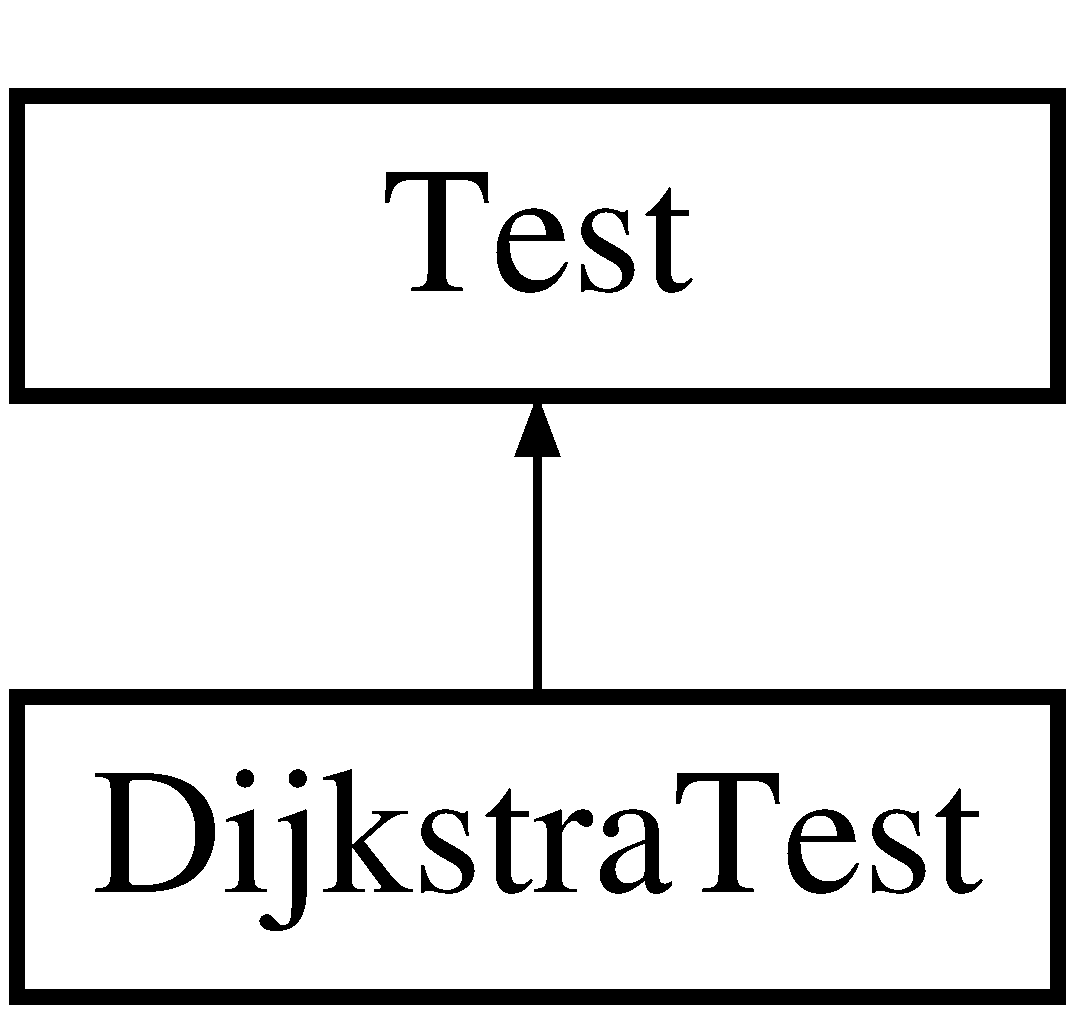
\includegraphics[height=2.000000cm]{class_dijkstra_test}
\end{center}
\end{figure}
\subsection*{Public Types}
\begin{DoxyCompactItemize}
\item 
typedef \hyperlink{struct_introduction_to_algorithm_1_1_graph_algorithm_1_1_graph}{Graph}$<$ D\+I\+J\+K\+\_\+\+N\+U\+M, \hyperlink{struct_introduction_to_algorithm_1_1_graph_algorithm_1_1_vertex_p}{Vertex\+P}$<$ int $>$ $>$ \hyperlink{class_dijkstra_test_af1d630aa34cb90e7bc11e2bcef82a2d7}{Graph\+Type}
\item 
typedef \hyperlink{struct_introduction_to_algorithm_1_1_graph_algorithm_1_1_vertex_p}{Vertex\+P}$<$ int $>$ \hyperlink{class_dijkstra_test_a00c55e6277edc6a0c52fc589df07d586}{Vertex\+Type}
\end{DoxyCompactItemize}
\subsection*{Protected Member Functions}
\begin{DoxyCompactItemize}
\item 
void \hyperlink{class_dijkstra_test_a112fd6757f4daff43c704f7f808a2ba4}{Set\+Up} ()
\item 
void \hyperlink{class_dijkstra_test_a8147e068ecc6561235948c254a4677a5}{Tear\+Down} ()
\end{DoxyCompactItemize}
\subsection*{Protected Attributes}
\begin{DoxyCompactItemize}
\item 
std\+::shared\+\_\+ptr$<$ \hyperlink{class_dijkstra_test_af1d630aa34cb90e7bc11e2bcef82a2d7}{Graph\+Type} $>$ \hyperlink{class_dijkstra_test_ad7c2ba728d52c2265fd629da2c9a383c}{\+\_\+1v\+\_\+graph}
\item 
std\+::shared\+\_\+ptr$<$ \hyperlink{class_dijkstra_test_af1d630aa34cb90e7bc11e2bcef82a2d7}{Graph\+Type} $>$ \hyperlink{class_dijkstra_test_ac99e2d7d0096e66a7abf7f1275b3a39a}{\+\_\+1e\+\_\+graph}
\item 
std\+::shared\+\_\+ptr$<$ \hyperlink{class_dijkstra_test_af1d630aa34cb90e7bc11e2bcef82a2d7}{Graph\+Type} $>$ \hyperlink{class_dijkstra_test_a7cdee342c58a60c71e394fd4c4ebfb94}{\+\_\+normal\+\_\+graph}
\end{DoxyCompactItemize}


\subsection{Detailed Description}
\hyperlink{class_dijkstra_test}{Dijkstra\+Test}\+:测试类,用于为测试提供基础数据 

{\ttfamily \hyperlink{class_dijkstra_test}{Dijkstra\+Test}}是 {\ttfamily \+::testing\+::\+Test} 的子类。它主要用于为每一个{\ttfamily T\+E\+S\+T\+\_\+\+F}准备测试环境 

Definition at line 40 of file dijkstra\+\_\+test.\+h.



\subsection{Member Typedef Documentation}
\hypertarget{class_dijkstra_test_af1d630aa34cb90e7bc11e2bcef82a2d7}{}\index{Dijkstra\+Test@{Dijkstra\+Test}!Graph\+Type@{Graph\+Type}}
\index{Graph\+Type@{Graph\+Type}!Dijkstra\+Test@{Dijkstra\+Test}}
\subsubsection[{Graph\+Type}]{\setlength{\rightskip}{0pt plus 5cm}typedef {\bf Graph}$<$D\+I\+J\+K\+\_\+\+N\+U\+M,{\bf Vertex\+P}$<$int$>$ $>$ {\bf Dijkstra\+Test\+::\+Graph\+Type}}\label{class_dijkstra_test_af1d630aa34cb90e7bc11e2bcef82a2d7}
模板实例化的图类型,该图的顶点类型为{\ttfamily Vertex\+P$<$int$>$} 

Definition at line 43 of file dijkstra\+\_\+test.\+h.

\hypertarget{class_dijkstra_test_a00c55e6277edc6a0c52fc589df07d586}{}\index{Dijkstra\+Test@{Dijkstra\+Test}!Vertex\+Type@{Vertex\+Type}}
\index{Vertex\+Type@{Vertex\+Type}!Dijkstra\+Test@{Dijkstra\+Test}}
\subsubsection[{Vertex\+Type}]{\setlength{\rightskip}{0pt plus 5cm}typedef {\bf Vertex\+P}$<$int$>$ {\bf Dijkstra\+Test\+::\+Vertex\+Type}}\label{class_dijkstra_test_a00c55e6277edc6a0c52fc589df07d586}
图的顶点类型为{\ttfamily Vertex\+P$<$int$>$} 

Definition at line 44 of file dijkstra\+\_\+test.\+h.



\subsection{Member Function Documentation}
\hypertarget{class_dijkstra_test_a112fd6757f4daff43c704f7f808a2ba4}{}\index{Dijkstra\+Test@{Dijkstra\+Test}!Set\+Up@{Set\+Up}}
\index{Set\+Up@{Set\+Up}!Dijkstra\+Test@{Dijkstra\+Test}}
\subsubsection[{Set\+Up()}]{\setlength{\rightskip}{0pt plus 5cm}void Dijkstra\+Test\+::\+Set\+Up (
\begin{DoxyParamCaption}
{}
\end{DoxyParamCaption}
)\hspace{0.3cm}{\ttfamily [inline]}, {\ttfamily [protected]}}\label{class_dijkstra_test_a112fd6757f4daff43c704f7f808a2ba4}


Definition at line 46 of file dijkstra\+\_\+test.\+h.

\hypertarget{class_dijkstra_test_a8147e068ecc6561235948c254a4677a5}{}\index{Dijkstra\+Test@{Dijkstra\+Test}!Tear\+Down@{Tear\+Down}}
\index{Tear\+Down@{Tear\+Down}!Dijkstra\+Test@{Dijkstra\+Test}}
\subsubsection[{Tear\+Down()}]{\setlength{\rightskip}{0pt plus 5cm}void Dijkstra\+Test\+::\+Tear\+Down (
\begin{DoxyParamCaption}
{}
\end{DoxyParamCaption}
)\hspace{0.3cm}{\ttfamily [inline]}, {\ttfamily [protected]}}\label{class_dijkstra_test_a8147e068ecc6561235948c254a4677a5}


Definition at line 64 of file dijkstra\+\_\+test.\+h.



\subsection{Member Data Documentation}
\hypertarget{class_dijkstra_test_ac99e2d7d0096e66a7abf7f1275b3a39a}{}\index{Dijkstra\+Test@{Dijkstra\+Test}!\+\_\+1e\+\_\+graph@{\+\_\+1e\+\_\+graph}}
\index{\+\_\+1e\+\_\+graph@{\+\_\+1e\+\_\+graph}!Dijkstra\+Test@{Dijkstra\+Test}}
\subsubsection[{\+\_\+1e\+\_\+graph}]{\setlength{\rightskip}{0pt plus 5cm}std\+::shared\+\_\+ptr$<${\bf Graph\+Type}$>$ Dijkstra\+Test\+::\+\_\+1e\+\_\+graph\hspace{0.3cm}{\ttfamily [protected]}}\label{class_dijkstra_test_ac99e2d7d0096e66a7abf7f1275b3a39a}
指向一个图,该图只有一条边 

Definition at line 67 of file dijkstra\+\_\+test.\+h.

\hypertarget{class_dijkstra_test_ad7c2ba728d52c2265fd629da2c9a383c}{}\index{Dijkstra\+Test@{Dijkstra\+Test}!\+\_\+1v\+\_\+graph@{\+\_\+1v\+\_\+graph}}
\index{\+\_\+1v\+\_\+graph@{\+\_\+1v\+\_\+graph}!Dijkstra\+Test@{Dijkstra\+Test}}
\subsubsection[{\+\_\+1v\+\_\+graph}]{\setlength{\rightskip}{0pt plus 5cm}std\+::shared\+\_\+ptr$<${\bf Graph\+Type}$>$ Dijkstra\+Test\+::\+\_\+1v\+\_\+graph\hspace{0.3cm}{\ttfamily [protected]}}\label{class_dijkstra_test_ad7c2ba728d52c2265fd629da2c9a383c}
指向一个图,该图只有一个顶点 

Definition at line 66 of file dijkstra\+\_\+test.\+h.

\hypertarget{class_dijkstra_test_a7cdee342c58a60c71e394fd4c4ebfb94}{}\index{Dijkstra\+Test@{Dijkstra\+Test}!\+\_\+normal\+\_\+graph@{\+\_\+normal\+\_\+graph}}
\index{\+\_\+normal\+\_\+graph@{\+\_\+normal\+\_\+graph}!Dijkstra\+Test@{Dijkstra\+Test}}
\subsubsection[{\+\_\+normal\+\_\+graph}]{\setlength{\rightskip}{0pt plus 5cm}std\+::shared\+\_\+ptr$<${\bf Graph\+Type}$>$ Dijkstra\+Test\+::\+\_\+normal\+\_\+graph\hspace{0.3cm}{\ttfamily [protected]}}\label{class_dijkstra_test_a7cdee342c58a60c71e394fd4c4ebfb94}
指向一个图,该图的边组成一条链条 

Definition at line 68 of file dijkstra\+\_\+test.\+h.



The documentation for this class was generated from the following file\+:\begin{DoxyCompactItemize}
\item 
src/graph\+\_\+algorithms/single\+\_\+source\+\_\+shortest\+\_\+path/dijkstra/\hyperlink{dijkstra__test_8h}{dijkstra\+\_\+test.\+h}\end{DoxyCompactItemize}

\hypertarget{struct_introduction_to_algorithm_1_1_set_algorithm_1_1_disjoint_set_node}{}\section{Introduction\+To\+Algorithm\+:\+:Set\+Algorithm\+:\+:Disjoint\+Set\+Node$<$ K\+Type $>$ Struct Template Reference}
\label{struct_introduction_to_algorithm_1_1_set_algorithm_1_1_disjoint_set_node}\index{Introduction\+To\+Algorithm\+::\+Set\+Algorithm\+::\+Disjoint\+Set\+Node$<$ K\+Type $>$@{Introduction\+To\+Algorithm\+::\+Set\+Algorithm\+::\+Disjoint\+Set\+Node$<$ K\+Type $>$}}


Disjoint\+Set\+Node:不相交集合森林的节点,算法导论第21章21.3节  




{\ttfamily \#include $<$disjointset.\+h$>$}

\subsection*{Public Types}
\begin{DoxyCompactItemize}
\item 
typedef K\+Type \hyperlink{struct_introduction_to_algorithm_1_1_set_algorithm_1_1_disjoint_set_node_a8f801679de129d80a99ad683430c534a}{Key\+Type}
\end{DoxyCompactItemize}
\subsection*{Public Member Functions}
\begin{DoxyCompactItemize}
\item 
\hyperlink{struct_introduction_to_algorithm_1_1_set_algorithm_1_1_disjoint_set_node_a579c4ac62902b32c0bd04ccea02536ea}{Disjoint\+Set\+Node} (std\+::shared\+\_\+ptr$<$ \hyperlink{struct_introduction_to_algorithm_1_1_set_algorithm_1_1_disjoint_set_node_a8f801679de129d80a99ad683430c534a}{Key\+Type} $>$v)
\begin{DoxyCompactList}\small\item\em Disjoint\+Set\+Node的显式构造函数 \end{DoxyCompactList}\end{DoxyCompactItemize}
\subsection*{Static Public Member Functions}
\begin{DoxyCompactItemize}
\item 
static std\+::shared\+\_\+ptr$<$ \hyperlink{struct_introduction_to_algorithm_1_1_set_algorithm_1_1_disjoint_set_node}{Disjoint\+Set\+Node} $>$ \hyperlink{struct_introduction_to_algorithm_1_1_set_algorithm_1_1_disjoint_set_node_a85fa0b8f80ba6529936ba2103c68194c}{find\+\_\+set} (std\+::shared\+\_\+ptr$<$ \hyperlink{struct_introduction_to_algorithm_1_1_set_algorithm_1_1_disjoint_set_node}{Disjoint\+Set\+Node} $>$node)
\begin{DoxyCompactList}\small\item\em find\+\_\+set:返回结点所在集合的代表结点 \end{DoxyCompactList}\item 
static void \hyperlink{struct_introduction_to_algorithm_1_1_set_algorithm_1_1_disjoint_set_node_a7346337c6f47bf066844c7101058cd92}{make\+\_\+set} (std\+::shared\+\_\+ptr$<$ \hyperlink{struct_introduction_to_algorithm_1_1_set_algorithm_1_1_disjoint_set_node}{Disjoint\+Set\+Node} $>$node)
\begin{DoxyCompactList}\small\item\em make\+\_\+set:创建集合 \end{DoxyCompactList}\item 
static void \hyperlink{struct_introduction_to_algorithm_1_1_set_algorithm_1_1_disjoint_set_node_ac5fff2fa07d82ed04529aa9159d37efc}{link\+\_\+set} (std\+::shared\+\_\+ptr$<$ \hyperlink{struct_introduction_to_algorithm_1_1_set_algorithm_1_1_disjoint_set_node}{Disjoint\+Set\+Node} $>$node\+X, std\+::shared\+\_\+ptr$<$ \hyperlink{struct_introduction_to_algorithm_1_1_set_algorithm_1_1_disjoint_set_node}{Disjoint\+Set\+Node} $>$node\+Y)
\begin{DoxyCompactList}\small\item\em link\+\_\+set:链接集合 \end{DoxyCompactList}\item 
static void \hyperlink{struct_introduction_to_algorithm_1_1_set_algorithm_1_1_disjoint_set_node_aeb6281c8d6ec20987015fb1d1421b309}{union\+\_\+set} (std\+::shared\+\_\+ptr$<$ \hyperlink{struct_introduction_to_algorithm_1_1_set_algorithm_1_1_disjoint_set_node}{Disjoint\+Set\+Node} $>$node\+X, std\+::shared\+\_\+ptr$<$ \hyperlink{struct_introduction_to_algorithm_1_1_set_algorithm_1_1_disjoint_set_node}{Disjoint\+Set\+Node} $>$node\+Y)
\begin{DoxyCompactList}\small\item\em union\+\_\+set:合并集合 \end{DoxyCompactList}\end{DoxyCompactItemize}
\subsection*{Public Attributes}
\begin{DoxyCompactItemize}
\item 
std\+::weak\+\_\+ptr$<$ \hyperlink{struct_introduction_to_algorithm_1_1_set_algorithm_1_1_disjoint_set_node_a8f801679de129d80a99ad683430c534a}{Key\+Type} $>$ \hyperlink{struct_introduction_to_algorithm_1_1_set_algorithm_1_1_disjoint_set_node_ae01535aa5e8ba05dceedd5c475d61c18}{value}
\item 
int \hyperlink{struct_introduction_to_algorithm_1_1_set_algorithm_1_1_disjoint_set_node_a1fd137f74ca1317bfb02d9e1640ce147}{rank}
\item 
std\+::shared\+\_\+ptr$<$ \hyperlink{struct_introduction_to_algorithm_1_1_set_algorithm_1_1_disjoint_set_node}{Disjoint\+Set\+Node} $>$ \hyperlink{struct_introduction_to_algorithm_1_1_set_algorithm_1_1_disjoint_set_node_ad5cf3f4d739ecd0c1f6d3b3005e21993}{parent}
\end{DoxyCompactItemize}


\subsection{Detailed Description}
\subsubsection*{template$<$typename K\+Type$>$struct Introduction\+To\+Algorithm\+::\+Set\+Algorithm\+::\+Disjoint\+Set\+Node$<$ K\+Type $>$}

Disjoint\+Set\+Node:不相交集合森林的节点,算法导论第21章21.3节 

一个不相交集合数据结构维护了一个不相交动态集的集合\{S1,S2,...Sk\}。我们用一个代表来标识每个集合,它是这个集合的某个成员。 不相交集合支持三个操作:(x,y等都是集合中的对象)


\begin{DoxyItemize}
\item make\+\_\+set(x)\+:建立一个新的集合,它的唯一成员是x
\item unionx(x,y)\+:将包含x和y的两个动态集合(表示为\+Sx和\+Sy)合并成一个新的集合。由于我们要求各个集合不相交,因此这里要消除原有的集合\+Sx和\+Sy。实际操作中, 我们把其中的一个集合的元素并入另一个集合中,来代替删除操作。
\item find\+\_\+set(x)\+:返回一个指针,该指针指向包含x的唯一集合的代表。
\end{DoxyItemize}

在某些图的算法中,图和不相交集数据结构的表示需要相互引用。即一个表示顶点的对象会包含一个指向与之对应的不相交集合对象的指针;反之亦然

不相交集合森林:不相交集合森林是不相交集合的一种更快的实现。用有根数来表示集合,树中的每个结点都包含一个成员,每棵树代表一个集合。 在不相交集合森林中,每个成员仅仅指向它的父节点。每棵树的根就是集合的代表并且它的父节点就是自己。

这里采用了启发式策略改进运行时间,使用了两种启发式策略:
\begin{DoxyItemize}
\item 按秩合并:每个结点x维持一个整数值属性rank,它代表了x的高度(从x到某一后代叶结点的最长简单路径上的结点数目)的一个上界。在按秩合并的union操作中, 我们让具有较小秩的根指向具有较大秩的根
\item 路径压缩:在{\ttfamily find\+\_\+set}操作中,使查找路径中的每个结点直接指向树根
\end{DoxyItemize}

如果单独采用按秩合并或者路径压缩,它们每一个都能改善不相交集合森林上操作的运行时间;而一起使用这两种启发式策略时,这种改善更大。 当同时使用按秩合并和路径压缩时,最坏情况下的运行时间为\+O(m$\ast$alpha$\ast$n)),这里alpha(n)是一个增长非常慢的函数。在任何一个可以想得到的不相交集合数据结构的应用中, alpha(n)$<$=4。其中n为结点个数,m为操作次数(运用了摊还分析) 

Definition at line 54 of file disjointset.\+h.



\subsection{Member Typedef Documentation}
\hypertarget{struct_introduction_to_algorithm_1_1_set_algorithm_1_1_disjoint_set_node_a8f801679de129d80a99ad683430c534a}{}\index{Introduction\+To\+Algorithm\+::\+Set\+Algorithm\+::\+Disjoint\+Set\+Node@{Introduction\+To\+Algorithm\+::\+Set\+Algorithm\+::\+Disjoint\+Set\+Node}!Key\+Type@{Key\+Type}}
\index{Key\+Type@{Key\+Type}!Introduction\+To\+Algorithm\+::\+Set\+Algorithm\+::\+Disjoint\+Set\+Node@{Introduction\+To\+Algorithm\+::\+Set\+Algorithm\+::\+Disjoint\+Set\+Node}}
\subsubsection[{Key\+Type}]{\setlength{\rightskip}{0pt plus 5cm}template$<$typename K\+Type $>$ typedef K\+Type {\bf Introduction\+To\+Algorithm\+::\+Set\+Algorithm\+::\+Disjoint\+Set\+Node}$<$ K\+Type $>$\+::{\bf Key\+Type}}\label{struct_introduction_to_algorithm_1_1_set_algorithm_1_1_disjoint_set_node_a8f801679de129d80a99ad683430c534a}
结点保存的数据类型 

Definition at line 56 of file disjointset.\+h.



\subsection{Constructor \& Destructor Documentation}
\hypertarget{struct_introduction_to_algorithm_1_1_set_algorithm_1_1_disjoint_set_node_a579c4ac62902b32c0bd04ccea02536ea}{}\index{Introduction\+To\+Algorithm\+::\+Set\+Algorithm\+::\+Disjoint\+Set\+Node@{Introduction\+To\+Algorithm\+::\+Set\+Algorithm\+::\+Disjoint\+Set\+Node}!Disjoint\+Set\+Node@{Disjoint\+Set\+Node}}
\index{Disjoint\+Set\+Node@{Disjoint\+Set\+Node}!Introduction\+To\+Algorithm\+::\+Set\+Algorithm\+::\+Disjoint\+Set\+Node@{Introduction\+To\+Algorithm\+::\+Set\+Algorithm\+::\+Disjoint\+Set\+Node}}
\subsubsection[{Disjoint\+Set\+Node(std\+::shared\+\_\+ptr$<$ Key\+Type $>$v)}]{\setlength{\rightskip}{0pt plus 5cm}template$<$typename K\+Type $>$ {\bf Introduction\+To\+Algorithm\+::\+Set\+Algorithm\+::\+Disjoint\+Set\+Node}$<$ K\+Type $>$\+::{\bf Disjoint\+Set\+Node} (
\begin{DoxyParamCaption}
\item[{std\+::shared\+\_\+ptr$<$ {\bf Key\+Type} $>$}]{v}
\end{DoxyParamCaption}
)\hspace{0.3cm}{\ttfamily [inline]}, {\ttfamily [explicit]}}\label{struct_introduction_to_algorithm_1_1_set_algorithm_1_1_disjoint_set_node_a579c4ac62902b32c0bd04ccea02536ea}


Disjoint\+Set\+Node的显式构造函数 


\begin{DoxyParams}{Parameters}
{\em v\+:结点保存的数据的指针} & 将v存入结点的value中 \\
\hline
\end{DoxyParams}


Definition at line 65 of file disjointset.\+h.



\subsection{Member Function Documentation}
\hypertarget{struct_introduction_to_algorithm_1_1_set_algorithm_1_1_disjoint_set_node_a85fa0b8f80ba6529936ba2103c68194c}{}\index{Introduction\+To\+Algorithm\+::\+Set\+Algorithm\+::\+Disjoint\+Set\+Node@{Introduction\+To\+Algorithm\+::\+Set\+Algorithm\+::\+Disjoint\+Set\+Node}!find\+\_\+set@{find\+\_\+set}}
\index{find\+\_\+set@{find\+\_\+set}!Introduction\+To\+Algorithm\+::\+Set\+Algorithm\+::\+Disjoint\+Set\+Node@{Introduction\+To\+Algorithm\+::\+Set\+Algorithm\+::\+Disjoint\+Set\+Node}}
\subsubsection[{find\+\_\+set(std\+::shared\+\_\+ptr$<$ Disjoint\+Set\+Node $>$node)}]{\setlength{\rightskip}{0pt plus 5cm}template$<$typename K\+Type $>$ static std\+::shared\+\_\+ptr$<${\bf Disjoint\+Set\+Node}$>$ {\bf Introduction\+To\+Algorithm\+::\+Set\+Algorithm\+::\+Disjoint\+Set\+Node}$<$ K\+Type $>$\+::find\+\_\+set (
\begin{DoxyParamCaption}
\item[{std\+::shared\+\_\+ptr$<$ {\bf Disjoint\+Set\+Node}$<$ K\+Type $>$ $>$}]{node}
\end{DoxyParamCaption}
)\hspace{0.3cm}{\ttfamily [inline]}, {\ttfamily [static]}}\label{struct_introduction_to_algorithm_1_1_set_algorithm_1_1_disjoint_set_node_a85fa0b8f80ba6529936ba2103c68194c}


find\+\_\+set:返回结点所在集合的代表结点 


\begin{DoxyParams}{Parameters}
{\em node\+:要查找的结点。它必须非空,否则抛出异常} & \\
\hline
\end{DoxyParams}
\begin{DoxyReturn}{Returns}
\+: 结点所在集合的代表结点的强指针
\end{DoxyReturn}
该操作简单沿着指向父节点的指针找到树的根。树的根的特征是:它的父节点就是它本身。 若结点不在不相交集合森林中(当结点的父节点指针为空时),则抛出异常。

find\+\_\+set过程是一个 two\+\_\+pass method,当它递归时,第一趟沿着查找路径向上直到找到树根; 当递归回溯时,第二趟沿着搜索树向下更新每个节点,使其父节点直接指向树根 

Definition at line 84 of file disjointset.\+h.

\hypertarget{struct_introduction_to_algorithm_1_1_set_algorithm_1_1_disjoint_set_node_ac5fff2fa07d82ed04529aa9159d37efc}{}\index{Introduction\+To\+Algorithm\+::\+Set\+Algorithm\+::\+Disjoint\+Set\+Node@{Introduction\+To\+Algorithm\+::\+Set\+Algorithm\+::\+Disjoint\+Set\+Node}!link\+\_\+set@{link\+\_\+set}}
\index{link\+\_\+set@{link\+\_\+set}!Introduction\+To\+Algorithm\+::\+Set\+Algorithm\+::\+Disjoint\+Set\+Node@{Introduction\+To\+Algorithm\+::\+Set\+Algorithm\+::\+Disjoint\+Set\+Node}}
\subsubsection[{link\+\_\+set(std\+::shared\+\_\+ptr$<$ Disjoint\+Set\+Node $>$node\+X, std\+::shared\+\_\+ptr$<$ Disjoint\+Set\+Node $>$node\+Y)}]{\setlength{\rightskip}{0pt plus 5cm}template$<$typename K\+Type $>$ static void {\bf Introduction\+To\+Algorithm\+::\+Set\+Algorithm\+::\+Disjoint\+Set\+Node}$<$ K\+Type $>$\+::link\+\_\+set (
\begin{DoxyParamCaption}
\item[{std\+::shared\+\_\+ptr$<$ {\bf Disjoint\+Set\+Node}$<$ K\+Type $>$ $>$}]{node\+X, }
\item[{std\+::shared\+\_\+ptr$<$ {\bf Disjoint\+Set\+Node}$<$ K\+Type $>$ $>$}]{node\+Y}
\end{DoxyParamCaption}
)\hspace{0.3cm}{\ttfamily [inline]}, {\ttfamily [static]}}\label{struct_introduction_to_algorithm_1_1_set_algorithm_1_1_disjoint_set_node_ac5fff2fa07d82ed04529aa9159d37efc}


link\+\_\+set:链接集合 


\begin{DoxyParams}{Parameters}
{\em node\+X\+:待链接的第一个集合中的根节点。} & \\
\hline
{\em node\+Y\+:待合并的第二个集合中的根节点} & 每个结点x维持一个整数值属性rank,它代表了x的高度(从x到某一后代叶结点的最长简单路径上的结点数目)的一个上界。在链接时我们让具有较小秩的根指向具有较大秩的根.\\
\hline
\end{DoxyParams}

\begin{DoxyItemize}
\item 如果 node\+X或者node\+Y为空,则直接返回
\item 如果 node\+X 和 node\+Y非空,但是node\+X或者node\+Y不是根结点,抛出异常 
\end{DoxyItemize}

Definition at line 124 of file disjointset.\+h.

\hypertarget{struct_introduction_to_algorithm_1_1_set_algorithm_1_1_disjoint_set_node_a7346337c6f47bf066844c7101058cd92}{}\index{Introduction\+To\+Algorithm\+::\+Set\+Algorithm\+::\+Disjoint\+Set\+Node@{Introduction\+To\+Algorithm\+::\+Set\+Algorithm\+::\+Disjoint\+Set\+Node}!make\+\_\+set@{make\+\_\+set}}
\index{make\+\_\+set@{make\+\_\+set}!Introduction\+To\+Algorithm\+::\+Set\+Algorithm\+::\+Disjoint\+Set\+Node@{Introduction\+To\+Algorithm\+::\+Set\+Algorithm\+::\+Disjoint\+Set\+Node}}
\subsubsection[{make\+\_\+set(std\+::shared\+\_\+ptr$<$ Disjoint\+Set\+Node $>$node)}]{\setlength{\rightskip}{0pt plus 5cm}template$<$typename K\+Type $>$ static void {\bf Introduction\+To\+Algorithm\+::\+Set\+Algorithm\+::\+Disjoint\+Set\+Node}$<$ K\+Type $>$\+::make\+\_\+set (
\begin{DoxyParamCaption}
\item[{std\+::shared\+\_\+ptr$<$ {\bf Disjoint\+Set\+Node}$<$ K\+Type $>$ $>$}]{node}
\end{DoxyParamCaption}
)\hspace{0.3cm}{\ttfamily [inline]}, {\ttfamily [static]}}\label{struct_introduction_to_algorithm_1_1_set_algorithm_1_1_disjoint_set_node_a7346337c6f47bf066844c7101058cd92}


make\+\_\+set:创建集合 


\begin{DoxyParams}{Parameters}
{\em node\+:创建集合的结点。它必须非空,否则抛出异常} & 该操作简单地创建一棵只有一个结点的树。它将树根的秩设为0,将树根的父节点指向树根本身 \\
\hline
\end{DoxyParams}


Definition at line 100 of file disjointset.\+h.

\hypertarget{struct_introduction_to_algorithm_1_1_set_algorithm_1_1_disjoint_set_node_aeb6281c8d6ec20987015fb1d1421b309}{}\index{Introduction\+To\+Algorithm\+::\+Set\+Algorithm\+::\+Disjoint\+Set\+Node@{Introduction\+To\+Algorithm\+::\+Set\+Algorithm\+::\+Disjoint\+Set\+Node}!union\+\_\+set@{union\+\_\+set}}
\index{union\+\_\+set@{union\+\_\+set}!Introduction\+To\+Algorithm\+::\+Set\+Algorithm\+::\+Disjoint\+Set\+Node@{Introduction\+To\+Algorithm\+::\+Set\+Algorithm\+::\+Disjoint\+Set\+Node}}
\subsubsection[{union\+\_\+set(std\+::shared\+\_\+ptr$<$ Disjoint\+Set\+Node $>$node\+X, std\+::shared\+\_\+ptr$<$ Disjoint\+Set\+Node $>$node\+Y)}]{\setlength{\rightskip}{0pt plus 5cm}template$<$typename K\+Type $>$ static void {\bf Introduction\+To\+Algorithm\+::\+Set\+Algorithm\+::\+Disjoint\+Set\+Node}$<$ K\+Type $>$\+::union\+\_\+set (
\begin{DoxyParamCaption}
\item[{std\+::shared\+\_\+ptr$<$ {\bf Disjoint\+Set\+Node}$<$ K\+Type $>$ $>$}]{node\+X, }
\item[{std\+::shared\+\_\+ptr$<$ {\bf Disjoint\+Set\+Node}$<$ K\+Type $>$ $>$}]{node\+Y}
\end{DoxyParamCaption}
)\hspace{0.3cm}{\ttfamily [inline]}, {\ttfamily [static]}}\label{struct_introduction_to_algorithm_1_1_set_algorithm_1_1_disjoint_set_node_aeb6281c8d6ec20987015fb1d1421b309}


union\+\_\+set:合并集合 


\begin{DoxyParams}{Parameters}
{\em node\+X\+:待合并的第一个集合中的某个结点} & \\
\hline
{\em node\+Y\+:待合并的第二个集合中的某个结点} & 该操作首先获取每个结点所在集合的代表结点,然后将它们合并起来 \\
\hline
\end{DoxyParams}


Definition at line 151 of file disjointset.\+h.



\subsection{Member Data Documentation}
\hypertarget{struct_introduction_to_algorithm_1_1_set_algorithm_1_1_disjoint_set_node_ad5cf3f4d739ecd0c1f6d3b3005e21993}{}\index{Introduction\+To\+Algorithm\+::\+Set\+Algorithm\+::\+Disjoint\+Set\+Node@{Introduction\+To\+Algorithm\+::\+Set\+Algorithm\+::\+Disjoint\+Set\+Node}!parent@{parent}}
\index{parent@{parent}!Introduction\+To\+Algorithm\+::\+Set\+Algorithm\+::\+Disjoint\+Set\+Node@{Introduction\+To\+Algorithm\+::\+Set\+Algorithm\+::\+Disjoint\+Set\+Node}}
\subsubsection[{parent}]{\setlength{\rightskip}{0pt plus 5cm}template$<$typename K\+Type $>$ std\+::shared\+\_\+ptr$<${\bf Disjoint\+Set\+Node}$>$ {\bf Introduction\+To\+Algorithm\+::\+Set\+Algorithm\+::\+Disjoint\+Set\+Node}$<$ K\+Type $>$\+::parent}\label{struct_introduction_to_algorithm_1_1_set_algorithm_1_1_disjoint_set_node_ad5cf3f4d739ecd0c1f6d3b3005e21993}
结点的父指针 

Definition at line 69 of file disjointset.\+h.

\hypertarget{struct_introduction_to_algorithm_1_1_set_algorithm_1_1_disjoint_set_node_a1fd137f74ca1317bfb02d9e1640ce147}{}\index{Introduction\+To\+Algorithm\+::\+Set\+Algorithm\+::\+Disjoint\+Set\+Node@{Introduction\+To\+Algorithm\+::\+Set\+Algorithm\+::\+Disjoint\+Set\+Node}!rank@{rank}}
\index{rank@{rank}!Introduction\+To\+Algorithm\+::\+Set\+Algorithm\+::\+Disjoint\+Set\+Node@{Introduction\+To\+Algorithm\+::\+Set\+Algorithm\+::\+Disjoint\+Set\+Node}}
\subsubsection[{rank}]{\setlength{\rightskip}{0pt plus 5cm}template$<$typename K\+Type $>$ int {\bf Introduction\+To\+Algorithm\+::\+Set\+Algorithm\+::\+Disjoint\+Set\+Node}$<$ K\+Type $>$\+::rank}\label{struct_introduction_to_algorithm_1_1_set_algorithm_1_1_disjoint_set_node_a1fd137f74ca1317bfb02d9e1640ce147}
结点的秩 

Definition at line 68 of file disjointset.\+h.

\hypertarget{struct_introduction_to_algorithm_1_1_set_algorithm_1_1_disjoint_set_node_ae01535aa5e8ba05dceedd5c475d61c18}{}\index{Introduction\+To\+Algorithm\+::\+Set\+Algorithm\+::\+Disjoint\+Set\+Node@{Introduction\+To\+Algorithm\+::\+Set\+Algorithm\+::\+Disjoint\+Set\+Node}!value@{value}}
\index{value@{value}!Introduction\+To\+Algorithm\+::\+Set\+Algorithm\+::\+Disjoint\+Set\+Node@{Introduction\+To\+Algorithm\+::\+Set\+Algorithm\+::\+Disjoint\+Set\+Node}}
\subsubsection[{value}]{\setlength{\rightskip}{0pt plus 5cm}template$<$typename K\+Type $>$ std\+::weak\+\_\+ptr$<${\bf Key\+Type}$>$ {\bf Introduction\+To\+Algorithm\+::\+Set\+Algorithm\+::\+Disjoint\+Set\+Node}$<$ K\+Type $>$\+::value}\label{struct_introduction_to_algorithm_1_1_set_algorithm_1_1_disjoint_set_node_ae01535aa5e8ba05dceedd5c475d61c18}
结点保存的数据的弱指针 

Definition at line 67 of file disjointset.\+h.



The documentation for this struct was generated from the following file\+:\begin{DoxyCompactItemize}
\item 
src/set\+\_\+algorithms/disjoint\+\_\+set/\hyperlink{disjointset_8h}{disjointset.\+h}\end{DoxyCompactItemize}

\hypertarget{class_disjoint_set_node_test}{}\section{Disjoint\+Set\+Node\+Test Class Reference}
\label{class_disjoint_set_node_test}\index{Disjoint\+Set\+Node\+Test@{Disjoint\+Set\+Node\+Test}}


\hyperlink{class_disjoint_set_node_test}{Disjoint\+Set\+Node\+Test}\+:测试类,用于为测试提供基础数据  




{\ttfamily \#include $<$disjointset\+\_\+test.\+h$>$}

Inheritance diagram for Disjoint\+Set\+Node\+Test\+:\begin{figure}[H]
\begin{center}
\leavevmode
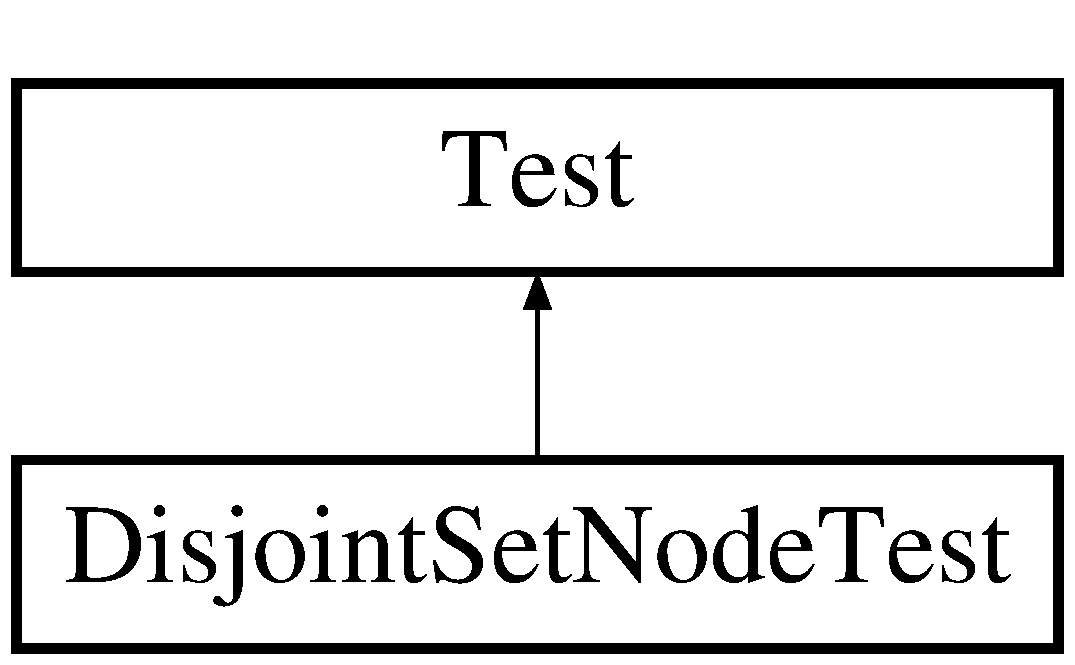
\includegraphics[height=2.000000cm]{class_disjoint_set_node_test}
\end{center}
\end{figure}
\subsection*{Public Types}
\begin{DoxyCompactItemize}
\item 
typedef \hyperlink{struct_introduction_to_algorithm_1_1_set_algorithm_1_1_disjoint_set_node}{Disjoint\+Set\+Node}$<$ int $>$ \hyperlink{class_disjoint_set_node_test_a2f0849289c8020ac6e4ef918b7f2cbde}{Node\+Type}
\end{DoxyCompactItemize}
\subsection*{Protected Member Functions}
\begin{DoxyCompactItemize}
\item 
void \hyperlink{class_disjoint_set_node_test_a6deb2278f038f2fb93f33c9415d757e9}{Set\+Up} ()
\item 
void \hyperlink{class_disjoint_set_node_test_ab6fd5a639f421653273b483a30a3e264}{Tear\+Down} ()
\end{DoxyCompactItemize}
\subsection*{Protected Attributes}
\begin{DoxyCompactItemize}
\item 
std\+::shared\+\_\+ptr$<$ \hyperlink{class_disjoint_set_node_test_a2f0849289c8020ac6e4ef918b7f2cbde}{Node\+Type} $>$ \hyperlink{class_disjoint_set_node_test_ae4bf8c2dd6ec1c63cdef65562fb5a278}{nodes} \mbox{[}S\+\_\+\+N\+U\+M\mbox{]}
\end{DoxyCompactItemize}


\subsection{Detailed Description}
\hyperlink{class_disjoint_set_node_test}{Disjoint\+Set\+Node\+Test}\+:测试类,用于为测试提供基础数据 

{\ttfamily \hyperlink{class_disjoint_set_node_test}{Disjoint\+Set\+Node\+Test}}是 {\ttfamily \+::testing\+::\+Test} 的子类。它主要用于为每一个{\ttfamily T\+E\+S\+T\+\_\+\+F}准备测试环境 

Definition at line 33 of file disjointset\+\_\+test.\+h.



\subsection{Member Typedef Documentation}
\hypertarget{class_disjoint_set_node_test_a2f0849289c8020ac6e4ef918b7f2cbde}{}\index{Disjoint\+Set\+Node\+Test@{Disjoint\+Set\+Node\+Test}!Node\+Type@{Node\+Type}}
\index{Node\+Type@{Node\+Type}!Disjoint\+Set\+Node\+Test@{Disjoint\+Set\+Node\+Test}}
\subsubsection[{Node\+Type}]{\setlength{\rightskip}{0pt plus 5cm}typedef {\bf Disjoint\+Set\+Node}$<$int$>$ {\bf Disjoint\+Set\+Node\+Test\+::\+Node\+Type}}\label{class_disjoint_set_node_test_a2f0849289c8020ac6e4ef918b7f2cbde}


Definition at line 36 of file disjointset\+\_\+test.\+h.



\subsection{Member Function Documentation}
\hypertarget{class_disjoint_set_node_test_a6deb2278f038f2fb93f33c9415d757e9}{}\index{Disjoint\+Set\+Node\+Test@{Disjoint\+Set\+Node\+Test}!Set\+Up@{Set\+Up}}
\index{Set\+Up@{Set\+Up}!Disjoint\+Set\+Node\+Test@{Disjoint\+Set\+Node\+Test}}
\subsubsection[{Set\+Up()}]{\setlength{\rightskip}{0pt plus 5cm}void Disjoint\+Set\+Node\+Test\+::\+Set\+Up (
\begin{DoxyParamCaption}
{}
\end{DoxyParamCaption}
)\hspace{0.3cm}{\ttfamily [inline]}, {\ttfamily [protected]}}\label{class_disjoint_set_node_test_a6deb2278f038f2fb93f33c9415d757e9}


Definition at line 38 of file disjointset\+\_\+test.\+h.

\hypertarget{class_disjoint_set_node_test_ab6fd5a639f421653273b483a30a3e264}{}\index{Disjoint\+Set\+Node\+Test@{Disjoint\+Set\+Node\+Test}!Tear\+Down@{Tear\+Down}}
\index{Tear\+Down@{Tear\+Down}!Disjoint\+Set\+Node\+Test@{Disjoint\+Set\+Node\+Test}}
\subsubsection[{Tear\+Down()}]{\setlength{\rightskip}{0pt plus 5cm}void Disjoint\+Set\+Node\+Test\+::\+Tear\+Down (
\begin{DoxyParamCaption}
{}
\end{DoxyParamCaption}
)\hspace{0.3cm}{\ttfamily [inline]}, {\ttfamily [protected]}}\label{class_disjoint_set_node_test_ab6fd5a639f421653273b483a30a3e264}


Definition at line 43 of file disjointset\+\_\+test.\+h.



\subsection{Member Data Documentation}
\hypertarget{class_disjoint_set_node_test_ae4bf8c2dd6ec1c63cdef65562fb5a278}{}\index{Disjoint\+Set\+Node\+Test@{Disjoint\+Set\+Node\+Test}!nodes@{nodes}}
\index{nodes@{nodes}!Disjoint\+Set\+Node\+Test@{Disjoint\+Set\+Node\+Test}}
\subsubsection[{nodes}]{\setlength{\rightskip}{0pt plus 5cm}std\+::shared\+\_\+ptr$<${\bf Node\+Type}$>$ Disjoint\+Set\+Node\+Test\+::nodes\mbox{[}S\+\_\+\+N\+U\+M\mbox{]}\hspace{0.3cm}{\ttfamily [protected]}}\label{class_disjoint_set_node_test_ae4bf8c2dd6ec1c63cdef65562fb5a278}
指向结点指针的数组 

Definition at line 44 of file disjointset\+\_\+test.\+h.



The documentation for this class was generated from the following file\+:\begin{DoxyCompactItemize}
\item 
src/set\+\_\+algorithms/disjoint\+\_\+set/\hyperlink{disjointset__test_8h}{disjointset\+\_\+test.\+h}\end{DoxyCompactItemize}

\hypertarget{struct_introduction_to_algorithm_1_1_graph_algorithm_1_1_edge}{}\section{Introduction\+To\+Algorithm\+:\+:Graph\+Algorithm\+:\+:Edge$<$ V\+Type $>$ Struct Template Reference}
\label{struct_introduction_to_algorithm_1_1_graph_algorithm_1_1_edge}\index{Introduction\+To\+Algorithm\+::\+Graph\+Algorithm\+::\+Edge$<$ V\+Type $>$@{Introduction\+To\+Algorithm\+::\+Graph\+Algorithm\+::\+Edge$<$ V\+Type $>$}}


Edge:图的边,算法导论22章22.1节  




{\ttfamily \#include $<$edge.\+h$>$}

\subsection*{Public Types}
\begin{DoxyCompactItemize}
\item 
typedef int \hyperlink{struct_introduction_to_algorithm_1_1_graph_algorithm_1_1_edge_a92b817240405b82f23dee4cdbefcb54f}{V\+I\+D\+Type}
\item 
typedef int \hyperlink{struct_introduction_to_algorithm_1_1_graph_algorithm_1_1_edge_a95cf631669c2a0d1bebb58ba2af110de}{E\+Weight\+Type}
\item 
typedef V\+Type \hyperlink{struct_introduction_to_algorithm_1_1_graph_algorithm_1_1_edge_a2a7bb332de66131ed664eb279c7ac1ed}{Vertex\+Type}
\item 
typedef std\+::tuple$<$ \hyperlink{struct_introduction_to_algorithm_1_1_graph_algorithm_1_1_edge_a92b817240405b82f23dee4cdbefcb54f}{V\+I\+D\+Type}, \hyperlink{struct_introduction_to_algorithm_1_1_graph_algorithm_1_1_edge_a92b817240405b82f23dee4cdbefcb54f}{V\+I\+D\+Type}, \hyperlink{struct_introduction_to_algorithm_1_1_graph_algorithm_1_1_edge_a95cf631669c2a0d1bebb58ba2af110de}{E\+Weight\+Type} $>$ \hyperlink{struct_introduction_to_algorithm_1_1_graph_algorithm_1_1_edge_a6cc12c05f7645ce74a6cff13b9ea932c}{Edge\+Tuple\+Type}
\end{DoxyCompactItemize}
\subsection*{Public Member Functions}
\begin{DoxyCompactItemize}
\item 
\hyperlink{struct_introduction_to_algorithm_1_1_graph_algorithm_1_1_edge_adf42723a706c3ff53b1d1bb612dfe03b}{Edge} (std\+::shared\+\_\+ptr$<$ \hyperlink{struct_introduction_to_algorithm_1_1_graph_algorithm_1_1_edge_a2a7bb332de66131ed664eb279c7ac1ed}{Vertex\+Type} $>$v1, std\+::shared\+\_\+ptr$<$ \hyperlink{struct_introduction_to_algorithm_1_1_graph_algorithm_1_1_edge_a2a7bb332de66131ed664eb279c7ac1ed}{Vertex\+Type} $>$v2, \hyperlink{struct_introduction_to_algorithm_1_1_graph_algorithm_1_1_edge_a95cf631669c2a0d1bebb58ba2af110de}{E\+Weight\+Type} w)
\begin{DoxyCompactList}\small\item\em 显式构造函数,必须指定两个顶点和一个权重 \end{DoxyCompactList}\item 
virtual std\+::string \hyperlink{struct_introduction_to_algorithm_1_1_graph_algorithm_1_1_edge_a9f7ecd0678638168991435c8370c8dae}{to\+\_\+string} () const 
\begin{DoxyCompactList}\small\item\em to\+\_\+string:返回边的字符串描述 \end{DoxyCompactList}\item 
const \hyperlink{struct_introduction_to_algorithm_1_1_graph_algorithm_1_1_edge_a6cc12c05f7645ce74a6cff13b9ea932c}{Edge\+Tuple\+Type} \hyperlink{struct_introduction_to_algorithm_1_1_graph_algorithm_1_1_edge_a1068057fa7240467e079d66a1a5edd7a}{edge\+\_\+tuple} () const 
\begin{DoxyCompactList}\small\item\em edge\+\_\+tuple:获取边的三元素元组 \end{DoxyCompactList}\end{DoxyCompactItemize}
\subsection*{Public Attributes}
\begin{DoxyCompactItemize}
\item 
std\+::shared\+\_\+ptr$<$ \hyperlink{struct_introduction_to_algorithm_1_1_graph_algorithm_1_1_edge_a2a7bb332de66131ed664eb279c7ac1ed}{Vertex\+Type} $>$ \hyperlink{struct_introduction_to_algorithm_1_1_graph_algorithm_1_1_edge_a634535a3f12be42c3c6ffb6d3c604fb7}{vertex1}
\item 
std\+::shared\+\_\+ptr$<$ \hyperlink{struct_introduction_to_algorithm_1_1_graph_algorithm_1_1_edge_a2a7bb332de66131ed664eb279c7ac1ed}{Vertex\+Type} $>$ \hyperlink{struct_introduction_to_algorithm_1_1_graph_algorithm_1_1_edge_a762ca9f6ad5abb1adf8b7e1319ea3b52}{vertex2}
\item 
\hyperlink{struct_introduction_to_algorithm_1_1_graph_algorithm_1_1_edge_a95cf631669c2a0d1bebb58ba2af110de}{E\+Weight\+Type} \hyperlink{struct_introduction_to_algorithm_1_1_graph_algorithm_1_1_edge_a139b40cb4524df195804bdce7a117164}{weight}
\end{DoxyCompactItemize}


\subsection{Detailed Description}
\subsubsection*{template$<$typename V\+Type$>$struct Introduction\+To\+Algorithm\+::\+Graph\+Algorithm\+::\+Edge$<$ V\+Type $>$}

Edge:图的边,算法导论22章22.1节 

边主要包含三个数据:


\begin{DoxyItemize}
\item {\ttfamily vertex1}:第一个顶点的强引用:
\item {\ttfamily vertex2}为第二个顶点的强引用。
\item {\ttfamily weight}\+: 边的权重(为int类型,可为正、负值)
\end{DoxyItemize}

为了便于计算,这里定义了一个元组,类型为{\ttfamily std\+::tuple$<$V\+I\+D\+Type,V\+I\+D\+Type,E\+Weight\+Type$>$},元组的第一个元素为第一个顶点的{\ttfamily id};元组的第二个元素为第二个顶点的{\ttfamily id}; 元组的第三个元素为边的权重。 

Definition at line 39 of file edge.\+h.



\subsection{Member Typedef Documentation}
\hypertarget{struct_introduction_to_algorithm_1_1_graph_algorithm_1_1_edge_a6cc12c05f7645ce74a6cff13b9ea932c}{}\index{Introduction\+To\+Algorithm\+::\+Graph\+Algorithm\+::\+Edge@{Introduction\+To\+Algorithm\+::\+Graph\+Algorithm\+::\+Edge}!Edge\+Tuple\+Type@{Edge\+Tuple\+Type}}
\index{Edge\+Tuple\+Type@{Edge\+Tuple\+Type}!Introduction\+To\+Algorithm\+::\+Graph\+Algorithm\+::\+Edge@{Introduction\+To\+Algorithm\+::\+Graph\+Algorithm\+::\+Edge}}
\subsubsection[{Edge\+Tuple\+Type}]{\setlength{\rightskip}{0pt plus 5cm}template$<$typename V\+Type $>$ typedef std\+::tuple$<${\bf V\+I\+D\+Type},{\bf V\+I\+D\+Type},{\bf E\+Weight\+Type}$>$ {\bf Introduction\+To\+Algorithm\+::\+Graph\+Algorithm\+::\+Edge}$<$ V\+Type $>$\+::{\bf Edge\+Tuple\+Type}}\label{struct_introduction_to_algorithm_1_1_graph_algorithm_1_1_edge_a6cc12c05f7645ce74a6cff13b9ea932c}
边的三元素(顶点1编号,顶点2编号,权重)组成的元组 

Definition at line 45 of file edge.\+h.

\hypertarget{struct_introduction_to_algorithm_1_1_graph_algorithm_1_1_edge_a95cf631669c2a0d1bebb58ba2af110de}{}\index{Introduction\+To\+Algorithm\+::\+Graph\+Algorithm\+::\+Edge@{Introduction\+To\+Algorithm\+::\+Graph\+Algorithm\+::\+Edge}!E\+Weight\+Type@{E\+Weight\+Type}}
\index{E\+Weight\+Type@{E\+Weight\+Type}!Introduction\+To\+Algorithm\+::\+Graph\+Algorithm\+::\+Edge@{Introduction\+To\+Algorithm\+::\+Graph\+Algorithm\+::\+Edge}}
\subsubsection[{E\+Weight\+Type}]{\setlength{\rightskip}{0pt plus 5cm}template$<$typename V\+Type $>$ typedef int {\bf Introduction\+To\+Algorithm\+::\+Graph\+Algorithm\+::\+Edge}$<$ V\+Type $>$\+::{\bf E\+Weight\+Type}}\label{struct_introduction_to_algorithm_1_1_graph_algorithm_1_1_edge_a95cf631669c2a0d1bebb58ba2af110de}
权重的类型 

Definition at line 43 of file edge.\+h.

\hypertarget{struct_introduction_to_algorithm_1_1_graph_algorithm_1_1_edge_a2a7bb332de66131ed664eb279c7ac1ed}{}\index{Introduction\+To\+Algorithm\+::\+Graph\+Algorithm\+::\+Edge@{Introduction\+To\+Algorithm\+::\+Graph\+Algorithm\+::\+Edge}!Vertex\+Type@{Vertex\+Type}}
\index{Vertex\+Type@{Vertex\+Type}!Introduction\+To\+Algorithm\+::\+Graph\+Algorithm\+::\+Edge@{Introduction\+To\+Algorithm\+::\+Graph\+Algorithm\+::\+Edge}}
\subsubsection[{Vertex\+Type}]{\setlength{\rightskip}{0pt plus 5cm}template$<$typename V\+Type $>$ typedef V\+Type {\bf Introduction\+To\+Algorithm\+::\+Graph\+Algorithm\+::\+Edge}$<$ V\+Type $>$\+::{\bf Vertex\+Type}}\label{struct_introduction_to_algorithm_1_1_graph_algorithm_1_1_edge_a2a7bb332de66131ed664eb279c7ac1ed}
顶点的类型 

Definition at line 44 of file edge.\+h.

\hypertarget{struct_introduction_to_algorithm_1_1_graph_algorithm_1_1_edge_a92b817240405b82f23dee4cdbefcb54f}{}\index{Introduction\+To\+Algorithm\+::\+Graph\+Algorithm\+::\+Edge@{Introduction\+To\+Algorithm\+::\+Graph\+Algorithm\+::\+Edge}!V\+I\+D\+Type@{V\+I\+D\+Type}}
\index{V\+I\+D\+Type@{V\+I\+D\+Type}!Introduction\+To\+Algorithm\+::\+Graph\+Algorithm\+::\+Edge@{Introduction\+To\+Algorithm\+::\+Graph\+Algorithm\+::\+Edge}}
\subsubsection[{V\+I\+D\+Type}]{\setlength{\rightskip}{0pt plus 5cm}template$<$typename V\+Type $>$ typedef int {\bf Introduction\+To\+Algorithm\+::\+Graph\+Algorithm\+::\+Edge}$<$ V\+Type $>$\+::{\bf V\+I\+D\+Type}}\label{struct_introduction_to_algorithm_1_1_graph_algorithm_1_1_edge_a92b817240405b82f23dee4cdbefcb54f}
顶点编号的类型 

Definition at line 42 of file edge.\+h.



\subsection{Constructor \& Destructor Documentation}
\hypertarget{struct_introduction_to_algorithm_1_1_graph_algorithm_1_1_edge_adf42723a706c3ff53b1d1bb612dfe03b}{}\index{Introduction\+To\+Algorithm\+::\+Graph\+Algorithm\+::\+Edge@{Introduction\+To\+Algorithm\+::\+Graph\+Algorithm\+::\+Edge}!Edge@{Edge}}
\index{Edge@{Edge}!Introduction\+To\+Algorithm\+::\+Graph\+Algorithm\+::\+Edge@{Introduction\+To\+Algorithm\+::\+Graph\+Algorithm\+::\+Edge}}
\subsubsection[{Edge(std\+::shared\+\_\+ptr$<$ Vertex\+Type $>$v1, std\+::shared\+\_\+ptr$<$ Vertex\+Type $>$v2, E\+Weight\+Type w)}]{\setlength{\rightskip}{0pt plus 5cm}template$<$typename V\+Type $>$ {\bf Introduction\+To\+Algorithm\+::\+Graph\+Algorithm\+::\+Edge}$<$ V\+Type $>$\+::{\bf Edge} (
\begin{DoxyParamCaption}
\item[{std\+::shared\+\_\+ptr$<$ {\bf Vertex\+Type} $>$}]{v1, }
\item[{std\+::shared\+\_\+ptr$<$ {\bf Vertex\+Type} $>$}]{v2, }
\item[{{\bf E\+Weight\+Type}}]{w}
\end{DoxyParamCaption}
)\hspace{0.3cm}{\ttfamily [inline]}}\label{struct_introduction_to_algorithm_1_1_graph_algorithm_1_1_edge_adf42723a706c3ff53b1d1bb612dfe03b}


显式构造函数,必须指定两个顶点和一个权重 


\begin{DoxyParams}{Parameters}
{\em v1\+:第一个顶点的强引用} & \\
\hline
{\em v2\+:第二个顶点的强引用} & \\
\hline
{\em w} & 边的权重 \\
\hline
\end{DoxyParams}


Definition at line 52 of file edge.\+h.



\subsection{Member Function Documentation}
\hypertarget{struct_introduction_to_algorithm_1_1_graph_algorithm_1_1_edge_a1068057fa7240467e079d66a1a5edd7a}{}\index{Introduction\+To\+Algorithm\+::\+Graph\+Algorithm\+::\+Edge@{Introduction\+To\+Algorithm\+::\+Graph\+Algorithm\+::\+Edge}!edge\+\_\+tuple@{edge\+\_\+tuple}}
\index{edge\+\_\+tuple@{edge\+\_\+tuple}!Introduction\+To\+Algorithm\+::\+Graph\+Algorithm\+::\+Edge@{Introduction\+To\+Algorithm\+::\+Graph\+Algorithm\+::\+Edge}}
\subsubsection[{edge\+\_\+tuple() const }]{\setlength{\rightskip}{0pt plus 5cm}template$<$typename V\+Type $>$ const {\bf Edge\+Tuple\+Type} {\bf Introduction\+To\+Algorithm\+::\+Graph\+Algorithm\+::\+Edge}$<$ V\+Type $>$\+::edge\+\_\+tuple (
\begin{DoxyParamCaption}
{}
\end{DoxyParamCaption}
) const\hspace{0.3cm}{\ttfamily [inline]}}\label{struct_introduction_to_algorithm_1_1_graph_algorithm_1_1_edge_a1068057fa7240467e079d66a1a5edd7a}


edge\+\_\+tuple:获取边的三元素元组 

\begin{DoxyReturn}{Returns}
\+:边的三元素元组 
\end{DoxyReturn}


Definition at line 72 of file edge.\+h.

\hypertarget{struct_introduction_to_algorithm_1_1_graph_algorithm_1_1_edge_a9f7ecd0678638168991435c8370c8dae}{}\index{Introduction\+To\+Algorithm\+::\+Graph\+Algorithm\+::\+Edge@{Introduction\+To\+Algorithm\+::\+Graph\+Algorithm\+::\+Edge}!to\+\_\+string@{to\+\_\+string}}
\index{to\+\_\+string@{to\+\_\+string}!Introduction\+To\+Algorithm\+::\+Graph\+Algorithm\+::\+Edge@{Introduction\+To\+Algorithm\+::\+Graph\+Algorithm\+::\+Edge}}
\subsubsection[{to\+\_\+string() const }]{\setlength{\rightskip}{0pt plus 5cm}template$<$typename V\+Type $>$ virtual std\+::string {\bf Introduction\+To\+Algorithm\+::\+Graph\+Algorithm\+::\+Edge}$<$ V\+Type $>$\+::to\+\_\+string (
\begin{DoxyParamCaption}
{}
\end{DoxyParamCaption}
) const\hspace{0.3cm}{\ttfamily [inline]}, {\ttfamily [virtual]}}\label{struct_introduction_to_algorithm_1_1_graph_algorithm_1_1_edge_a9f7ecd0678638168991435c8370c8dae}


to\+\_\+string:返回边的字符串描述 

\begin{DoxyReturn}{Returns}
\+:边的字符串描述 
\end{DoxyReturn}


Definition at line 62 of file edge.\+h.



\subsection{Member Data Documentation}
\hypertarget{struct_introduction_to_algorithm_1_1_graph_algorithm_1_1_edge_a634535a3f12be42c3c6ffb6d3c604fb7}{}\index{Introduction\+To\+Algorithm\+::\+Graph\+Algorithm\+::\+Edge@{Introduction\+To\+Algorithm\+::\+Graph\+Algorithm\+::\+Edge}!vertex1@{vertex1}}
\index{vertex1@{vertex1}!Introduction\+To\+Algorithm\+::\+Graph\+Algorithm\+::\+Edge@{Introduction\+To\+Algorithm\+::\+Graph\+Algorithm\+::\+Edge}}
\subsubsection[{vertex1}]{\setlength{\rightskip}{0pt plus 5cm}template$<$typename V\+Type $>$ std\+::shared\+\_\+ptr$<${\bf Vertex\+Type}$>$ {\bf Introduction\+To\+Algorithm\+::\+Graph\+Algorithm\+::\+Edge}$<$ V\+Type $>$\+::vertex1}\label{struct_introduction_to_algorithm_1_1_graph_algorithm_1_1_edge_a634535a3f12be42c3c6ffb6d3c604fb7}
边的第一个顶点 

Definition at line 76 of file edge.\+h.

\hypertarget{struct_introduction_to_algorithm_1_1_graph_algorithm_1_1_edge_a762ca9f6ad5abb1adf8b7e1319ea3b52}{}\index{Introduction\+To\+Algorithm\+::\+Graph\+Algorithm\+::\+Edge@{Introduction\+To\+Algorithm\+::\+Graph\+Algorithm\+::\+Edge}!vertex2@{vertex2}}
\index{vertex2@{vertex2}!Introduction\+To\+Algorithm\+::\+Graph\+Algorithm\+::\+Edge@{Introduction\+To\+Algorithm\+::\+Graph\+Algorithm\+::\+Edge}}
\subsubsection[{vertex2}]{\setlength{\rightskip}{0pt plus 5cm}template$<$typename V\+Type $>$ std\+::shared\+\_\+ptr$<${\bf Vertex\+Type}$>$ {\bf Introduction\+To\+Algorithm\+::\+Graph\+Algorithm\+::\+Edge}$<$ V\+Type $>$\+::vertex2}\label{struct_introduction_to_algorithm_1_1_graph_algorithm_1_1_edge_a762ca9f6ad5abb1adf8b7e1319ea3b52}
边的第二个顶点 

Definition at line 77 of file edge.\+h.

\hypertarget{struct_introduction_to_algorithm_1_1_graph_algorithm_1_1_edge_a139b40cb4524df195804bdce7a117164}{}\index{Introduction\+To\+Algorithm\+::\+Graph\+Algorithm\+::\+Edge@{Introduction\+To\+Algorithm\+::\+Graph\+Algorithm\+::\+Edge}!weight@{weight}}
\index{weight@{weight}!Introduction\+To\+Algorithm\+::\+Graph\+Algorithm\+::\+Edge@{Introduction\+To\+Algorithm\+::\+Graph\+Algorithm\+::\+Edge}}
\subsubsection[{weight}]{\setlength{\rightskip}{0pt plus 5cm}template$<$typename V\+Type $>$ {\bf E\+Weight\+Type} {\bf Introduction\+To\+Algorithm\+::\+Graph\+Algorithm\+::\+Edge}$<$ V\+Type $>$\+::weight}\label{struct_introduction_to_algorithm_1_1_graph_algorithm_1_1_edge_a139b40cb4524df195804bdce7a117164}
边的权重 

Definition at line 78 of file edge.\+h.



The documentation for this struct was generated from the following file\+:\begin{DoxyCompactItemize}
\item 
src/graph\+\_\+algorithms/basic\+\_\+graph/graph\+\_\+representation/graph\+\_\+edge/\hyperlink{edge_8h}{edge.\+h}\end{DoxyCompactItemize}

\hypertarget{class_edge_test}{}\section{Edge\+Test Class Reference}
\label{class_edge_test}\index{Edge\+Test@{Edge\+Test}}


\hyperlink{class_edge_test}{Edge\+Test}\+:测试类,用于为测试{\ttfamily Edge}提供基础数据  




{\ttfamily \#include $<$edge\+\_\+test.\+h$>$}

Inheritance diagram for Edge\+Test\+:\begin{figure}[H]
\begin{center}
\leavevmode
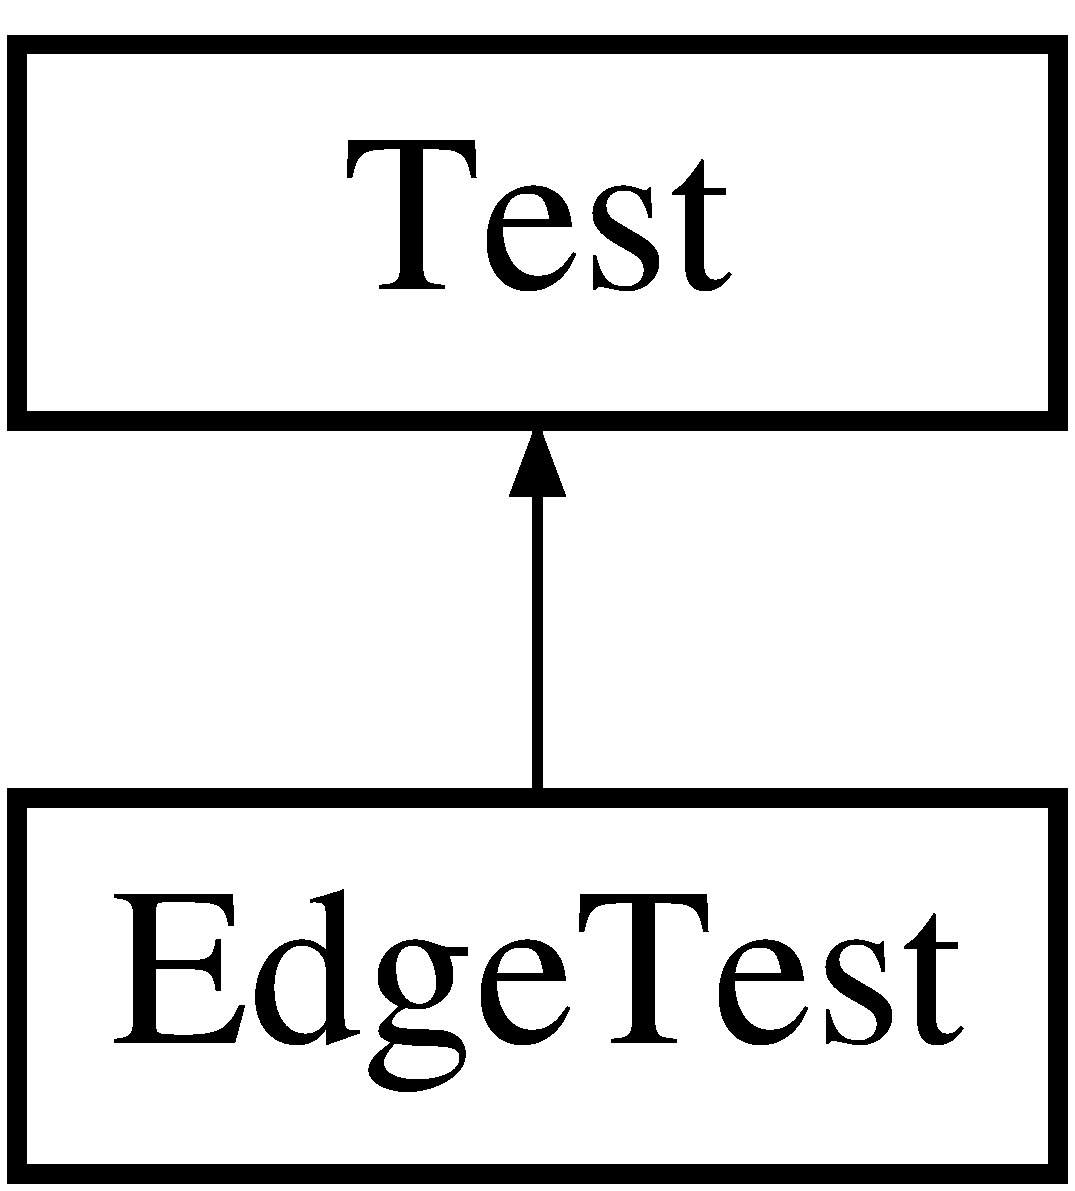
\includegraphics[height=2.000000cm]{class_edge_test}
\end{center}
\end{figure}
\subsection*{Public Types}
\begin{DoxyCompactItemize}
\item 
typedef \hyperlink{struct_introduction_to_algorithm_1_1_graph_algorithm_1_1_vertex}{Vertex}$<$ double $>$ \hyperlink{class_edge_test_a983bfc4e56ab07fc54c55f71815d39e6}{Node}
\end{DoxyCompactItemize}
\subsection*{Protected Member Functions}
\begin{DoxyCompactItemize}
\item 
void \hyperlink{class_edge_test_af1f1a79b9cc810c2548e1d2d0071f1bc}{Set\+Up} ()
\item 
void \hyperlink{class_edge_test_a14e4e78eddefbfedeebeb075fa74cbad}{Tear\+Down} ()
\end{DoxyCompactItemize}
\subsection*{Protected Attributes}
\begin{DoxyCompactItemize}
\item 
std\+::shared\+\_\+ptr$<$ \hyperlink{struct_introduction_to_algorithm_1_1_graph_algorithm_1_1_edge}{Edge}$<$ \hyperlink{class_edge_test_a983bfc4e56ab07fc54c55f71815d39e6}{Node} $>$ $>$ \hyperlink{class_edge_test_a8ab903577f2907ee1110d5f5f4d16b83}{\+\_\+edge}
\end{DoxyCompactItemize}


\subsection{Detailed Description}
\hyperlink{class_edge_test}{Edge\+Test}\+:测试类,用于为测试{\ttfamily Edge}提供基础数据 

{\ttfamily \hyperlink{class_edge_test}{Edge\+Test}}是 {\ttfamily \+::testing\+::\+Test} 的子类。它主要用于为每一个{\ttfamily T\+E\+S\+T\+\_\+\+F}准备测试环境 

Definition at line 32 of file edge\+\_\+test.\+h.



\subsection{Member Typedef Documentation}
\hypertarget{class_edge_test_a983bfc4e56ab07fc54c55f71815d39e6}{}\index{Edge\+Test@{Edge\+Test}!Node@{Node}}
\index{Node@{Node}!Edge\+Test@{Edge\+Test}}
\subsubsection[{Node}]{\setlength{\rightskip}{0pt plus 5cm}typedef {\bf Vertex}$<$double$>$ {\bf Edge\+Test\+::\+Node}}\label{class_edge_test_a983bfc4e56ab07fc54c55f71815d39e6}


Definition at line 35 of file edge\+\_\+test.\+h.



\subsection{Member Function Documentation}
\hypertarget{class_edge_test_af1f1a79b9cc810c2548e1d2d0071f1bc}{}\index{Edge\+Test@{Edge\+Test}!Set\+Up@{Set\+Up}}
\index{Set\+Up@{Set\+Up}!Edge\+Test@{Edge\+Test}}
\subsubsection[{Set\+Up()}]{\setlength{\rightskip}{0pt plus 5cm}void Edge\+Test\+::\+Set\+Up (
\begin{DoxyParamCaption}
{}
\end{DoxyParamCaption}
)\hspace{0.3cm}{\ttfamily [inline]}, {\ttfamily [protected]}}\label{class_edge_test_af1f1a79b9cc810c2548e1d2d0071f1bc}


Definition at line 37 of file edge\+\_\+test.\+h.

\hypertarget{class_edge_test_a14e4e78eddefbfedeebeb075fa74cbad}{}\index{Edge\+Test@{Edge\+Test}!Tear\+Down@{Tear\+Down}}
\index{Tear\+Down@{Tear\+Down}!Edge\+Test@{Edge\+Test}}
\subsubsection[{Tear\+Down()}]{\setlength{\rightskip}{0pt plus 5cm}void Edge\+Test\+::\+Tear\+Down (
\begin{DoxyParamCaption}
{}
\end{DoxyParamCaption}
)\hspace{0.3cm}{\ttfamily [inline]}, {\ttfamily [protected]}}\label{class_edge_test_a14e4e78eddefbfedeebeb075fa74cbad}


Definition at line 40 of file edge\+\_\+test.\+h.



\subsection{Member Data Documentation}
\hypertarget{class_edge_test_a8ab903577f2907ee1110d5f5f4d16b83}{}\index{Edge\+Test@{Edge\+Test}!\+\_\+edge@{\+\_\+edge}}
\index{\+\_\+edge@{\+\_\+edge}!Edge\+Test@{Edge\+Test}}
\subsubsection[{\+\_\+edge}]{\setlength{\rightskip}{0pt plus 5cm}std\+::shared\+\_\+ptr$<${\bf Edge}$<${\bf Node}$>$ $>$ Edge\+Test\+::\+\_\+edge\hspace{0.3cm}{\ttfamily [protected]}}\label{class_edge_test_a8ab903577f2907ee1110d5f5f4d16b83}
指向一条边 

Definition at line 42 of file edge\+\_\+test.\+h.



The documentation for this class was generated from the following file\+:\begin{DoxyCompactItemize}
\item 
src/graph\+\_\+algorithms/basic\+\_\+graph/graph\+\_\+representation/graph\+\_\+edge/\hyperlink{edge__test_8h}{edge\+\_\+test.\+h}\end{DoxyCompactItemize}

\hypertarget{struct_introduction_to_algorithm_1_1_graph_algorithm_1_1_flow_vertex}{}\section{Introduction\+To\+Algorithm\+:\+:Graph\+Algorithm\+:\+:Flow\+Vertex$<$ K\+Type $>$ Struct Template Reference}
\label{struct_introduction_to_algorithm_1_1_graph_algorithm_1_1_flow_vertex}\index{Introduction\+To\+Algorithm\+::\+Graph\+Algorithm\+::\+Flow\+Vertex$<$ K\+Type $>$@{Introduction\+To\+Algorithm\+::\+Graph\+Algorithm\+::\+Flow\+Vertex$<$ K\+Type $>$}}


Flow\+Vertex:推送-\/重贴标签算法图的顶点,算法导论26章26.4节  




{\ttfamily \#include $<$flow\+\_\+vertex.\+h$>$}

Inheritance diagram for Introduction\+To\+Algorithm\+:\+:Graph\+Algorithm\+:\+:Flow\+Vertex$<$ K\+Type $>$\+:\begin{figure}[H]
\begin{center}
\leavevmode
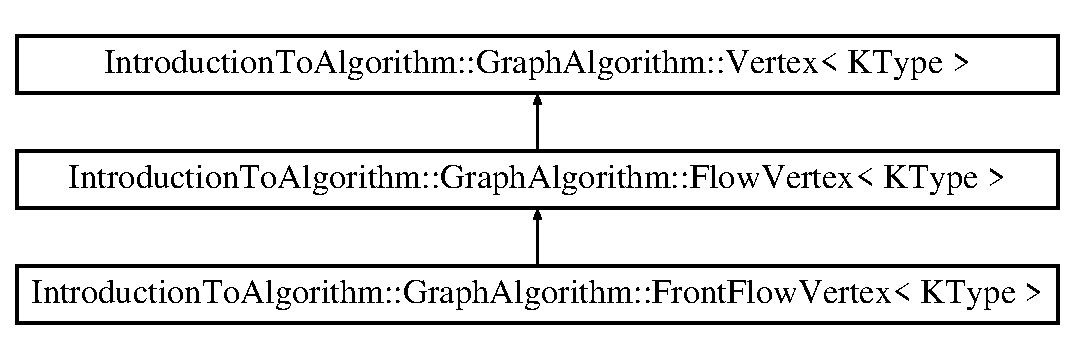
\includegraphics[height=3.000000cm]{struct_introduction_to_algorithm_1_1_graph_algorithm_1_1_flow_vertex}
\end{center}
\end{figure}
\subsection*{Public Types}
\begin{DoxyCompactItemize}
\item 
typedef K\+Type \hyperlink{struct_introduction_to_algorithm_1_1_graph_algorithm_1_1_flow_vertex_a014b25c20124a24525ef7db0588466b9}{Key\+Type}
\item 
typedef int \hyperlink{struct_introduction_to_algorithm_1_1_graph_algorithm_1_1_flow_vertex_ae48ab0918590bd6a6763d007694ff161}{V\+I\+D\+Type}
\end{DoxyCompactItemize}
\subsection*{Public Member Functions}
\begin{DoxyCompactItemize}
\item 
\hyperlink{struct_introduction_to_algorithm_1_1_graph_algorithm_1_1_flow_vertex_a19355adc725984f1ae28f254b6ba9bd7}{Flow\+Vertex} ()
\begin{DoxyCompactList}\small\item\em 默认构造函数 \end{DoxyCompactList}\item 
\hyperlink{struct_introduction_to_algorithm_1_1_graph_algorithm_1_1_flow_vertex_a4593a33cdfec0ecf40f9908d4fee5e00}{Flow\+Vertex} (const \hyperlink{struct_introduction_to_algorithm_1_1_graph_algorithm_1_1_flow_vertex_a014b25c20124a24525ef7db0588466b9}{Key\+Type} \&k)
\begin{DoxyCompactList}\small\item\em 显式构造函数,指定{\ttfamily key} \end{DoxyCompactList}\item 
\hyperlink{struct_introduction_to_algorithm_1_1_graph_algorithm_1_1_flow_vertex_a49bbf9ed3ed8769337403d455c383a4f}{Flow\+Vertex} (const \hyperlink{struct_introduction_to_algorithm_1_1_graph_algorithm_1_1_flow_vertex_a014b25c20124a24525ef7db0588466b9}{Key\+Type} \&k, \hyperlink{struct_introduction_to_algorithm_1_1_graph_algorithm_1_1_flow_vertex_ae48ab0918590bd6a6763d007694ff161}{V\+I\+D\+Type} d)
\begin{DoxyCompactList}\small\item\em 显式构造函数,指定{\ttfamily key}和编号 \end{DoxyCompactList}\item 
virtual std\+::string \hyperlink{struct_introduction_to_algorithm_1_1_graph_algorithm_1_1_flow_vertex_aa373a13a1fdee1fdcdbd0b55eaa1d1fb}{to\+\_\+string} () const 
\begin{DoxyCompactList}\small\item\em to\+\_\+string:返回顶点的字符串描述 \end{DoxyCompactList}\end{DoxyCompactItemize}
\subsection*{Public Attributes}
\begin{DoxyCompactItemize}
\item 
int \hyperlink{struct_introduction_to_algorithm_1_1_graph_algorithm_1_1_flow_vertex_a05f50003725449bbc9f4ee929c9ea87a}{h}
\end{DoxyCompactItemize}


\subsection{Detailed Description}
\subsubsection*{template$<$typename K\+Type$>$struct Introduction\+To\+Algorithm\+::\+Graph\+Algorithm\+::\+Flow\+Vertex$<$ K\+Type $>$}

Flow\+Vertex:推送-\/重贴标签算法图的顶点,算法导论26章26.4节 

\hyperlink{struct_introduction_to_algorithm_1_1_graph_algorithm_1_1_flow_vertex}{Flow\+Vertex} 是 Vertex的子类。它比\+Vertex多了一个{\ttfamily int h} 成员变量。其中:


\begin{DoxyItemize}
\item {\ttfamily K\+Type key}:表示顶点的超额流量
\item {\ttfamily int h}:表示顶点的高度 
\end{DoxyItemize}

Definition at line 34 of file flow\+\_\+vertex.\+h.



\subsection{Member Typedef Documentation}
\hypertarget{struct_introduction_to_algorithm_1_1_graph_algorithm_1_1_flow_vertex_a014b25c20124a24525ef7db0588466b9}{}\index{Introduction\+To\+Algorithm\+::\+Graph\+Algorithm\+::\+Flow\+Vertex@{Introduction\+To\+Algorithm\+::\+Graph\+Algorithm\+::\+Flow\+Vertex}!Key\+Type@{Key\+Type}}
\index{Key\+Type@{Key\+Type}!Introduction\+To\+Algorithm\+::\+Graph\+Algorithm\+::\+Flow\+Vertex@{Introduction\+To\+Algorithm\+::\+Graph\+Algorithm\+::\+Flow\+Vertex}}
\subsubsection[{Key\+Type}]{\setlength{\rightskip}{0pt plus 5cm}template$<$typename K\+Type$>$ typedef K\+Type {\bf Introduction\+To\+Algorithm\+::\+Graph\+Algorithm\+::\+Flow\+Vertex}$<$ K\+Type $>$\+::{\bf Key\+Type}}\label{struct_introduction_to_algorithm_1_1_graph_algorithm_1_1_flow_vertex_a014b25c20124a24525ef7db0588466b9}
顶点存储数据的类型 

Definition at line 36 of file flow\+\_\+vertex.\+h.

\hypertarget{struct_introduction_to_algorithm_1_1_graph_algorithm_1_1_flow_vertex_ae48ab0918590bd6a6763d007694ff161}{}\index{Introduction\+To\+Algorithm\+::\+Graph\+Algorithm\+::\+Flow\+Vertex@{Introduction\+To\+Algorithm\+::\+Graph\+Algorithm\+::\+Flow\+Vertex}!V\+I\+D\+Type@{V\+I\+D\+Type}}
\index{V\+I\+D\+Type@{V\+I\+D\+Type}!Introduction\+To\+Algorithm\+::\+Graph\+Algorithm\+::\+Flow\+Vertex@{Introduction\+To\+Algorithm\+::\+Graph\+Algorithm\+::\+Flow\+Vertex}}
\subsubsection[{V\+I\+D\+Type}]{\setlength{\rightskip}{0pt plus 5cm}template$<$typename K\+Type$>$ typedef int {\bf Introduction\+To\+Algorithm\+::\+Graph\+Algorithm\+::\+Flow\+Vertex}$<$ K\+Type $>$\+::{\bf V\+I\+D\+Type}}\label{struct_introduction_to_algorithm_1_1_graph_algorithm_1_1_flow_vertex_ae48ab0918590bd6a6763d007694ff161}
顶点编号的数据类型 

Definition at line 37 of file flow\+\_\+vertex.\+h.



\subsection{Constructor \& Destructor Documentation}
\hypertarget{struct_introduction_to_algorithm_1_1_graph_algorithm_1_1_flow_vertex_a19355adc725984f1ae28f254b6ba9bd7}{}\index{Introduction\+To\+Algorithm\+::\+Graph\+Algorithm\+::\+Flow\+Vertex@{Introduction\+To\+Algorithm\+::\+Graph\+Algorithm\+::\+Flow\+Vertex}!Flow\+Vertex@{Flow\+Vertex}}
\index{Flow\+Vertex@{Flow\+Vertex}!Introduction\+To\+Algorithm\+::\+Graph\+Algorithm\+::\+Flow\+Vertex@{Introduction\+To\+Algorithm\+::\+Graph\+Algorithm\+::\+Flow\+Vertex}}
\subsubsection[{Flow\+Vertex()}]{\setlength{\rightskip}{0pt plus 5cm}template$<$typename K\+Type$>$ {\bf Introduction\+To\+Algorithm\+::\+Graph\+Algorithm\+::\+Flow\+Vertex}$<$ K\+Type $>$\+::{\bf Flow\+Vertex} (
\begin{DoxyParamCaption}
{}
\end{DoxyParamCaption}
)\hspace{0.3cm}{\ttfamily [inline]}}\label{struct_introduction_to_algorithm_1_1_graph_algorithm_1_1_flow_vertex_a19355adc725984f1ae28f254b6ba9bd7}


默认构造函数 



Definition at line 40 of file flow\+\_\+vertex.\+h.

\hypertarget{struct_introduction_to_algorithm_1_1_graph_algorithm_1_1_flow_vertex_a4593a33cdfec0ecf40f9908d4fee5e00}{}\index{Introduction\+To\+Algorithm\+::\+Graph\+Algorithm\+::\+Flow\+Vertex@{Introduction\+To\+Algorithm\+::\+Graph\+Algorithm\+::\+Flow\+Vertex}!Flow\+Vertex@{Flow\+Vertex}}
\index{Flow\+Vertex@{Flow\+Vertex}!Introduction\+To\+Algorithm\+::\+Graph\+Algorithm\+::\+Flow\+Vertex@{Introduction\+To\+Algorithm\+::\+Graph\+Algorithm\+::\+Flow\+Vertex}}
\subsubsection[{Flow\+Vertex(const Key\+Type \&k)}]{\setlength{\rightskip}{0pt plus 5cm}template$<$typename K\+Type$>$ {\bf Introduction\+To\+Algorithm\+::\+Graph\+Algorithm\+::\+Flow\+Vertex}$<$ K\+Type $>$\+::{\bf Flow\+Vertex} (
\begin{DoxyParamCaption}
\item[{const {\bf Key\+Type} \&}]{k}
\end{DoxyParamCaption}
)\hspace{0.3cm}{\ttfamily [inline]}, {\ttfamily [explicit]}}\label{struct_introduction_to_algorithm_1_1_graph_algorithm_1_1_flow_vertex_a4593a33cdfec0ecf40f9908d4fee5e00}


显式构造函数,指定{\ttfamily key} 


\begin{DoxyParams}{Parameters}
{\em k\+:顶点存放的数据} & \\
\hline
\end{DoxyParams}


Definition at line 45 of file flow\+\_\+vertex.\+h.

\hypertarget{struct_introduction_to_algorithm_1_1_graph_algorithm_1_1_flow_vertex_a49bbf9ed3ed8769337403d455c383a4f}{}\index{Introduction\+To\+Algorithm\+::\+Graph\+Algorithm\+::\+Flow\+Vertex@{Introduction\+To\+Algorithm\+::\+Graph\+Algorithm\+::\+Flow\+Vertex}!Flow\+Vertex@{Flow\+Vertex}}
\index{Flow\+Vertex@{Flow\+Vertex}!Introduction\+To\+Algorithm\+::\+Graph\+Algorithm\+::\+Flow\+Vertex@{Introduction\+To\+Algorithm\+::\+Graph\+Algorithm\+::\+Flow\+Vertex}}
\subsubsection[{Flow\+Vertex(const Key\+Type \&k, V\+I\+D\+Type d)}]{\setlength{\rightskip}{0pt plus 5cm}template$<$typename K\+Type$>$ {\bf Introduction\+To\+Algorithm\+::\+Graph\+Algorithm\+::\+Flow\+Vertex}$<$ K\+Type $>$\+::{\bf Flow\+Vertex} (
\begin{DoxyParamCaption}
\item[{const {\bf Key\+Type} \&}]{k, }
\item[{{\bf V\+I\+D\+Type}}]{d}
\end{DoxyParamCaption}
)\hspace{0.3cm}{\ttfamily [inline]}}\label{struct_introduction_to_algorithm_1_1_graph_algorithm_1_1_flow_vertex_a49bbf9ed3ed8769337403d455c383a4f}


显式构造函数,指定{\ttfamily key}和编号 


\begin{DoxyParams}{Parameters}
{\em k\+:顶点存放的数据} & \\
\hline
{\em d\+:顶点的编号} & \\
\hline
\end{DoxyParams}


Definition at line 51 of file flow\+\_\+vertex.\+h.



\subsection{Member Function Documentation}
\hypertarget{struct_introduction_to_algorithm_1_1_graph_algorithm_1_1_flow_vertex_aa373a13a1fdee1fdcdbd0b55eaa1d1fb}{}\index{Introduction\+To\+Algorithm\+::\+Graph\+Algorithm\+::\+Flow\+Vertex@{Introduction\+To\+Algorithm\+::\+Graph\+Algorithm\+::\+Flow\+Vertex}!to\+\_\+string@{to\+\_\+string}}
\index{to\+\_\+string@{to\+\_\+string}!Introduction\+To\+Algorithm\+::\+Graph\+Algorithm\+::\+Flow\+Vertex@{Introduction\+To\+Algorithm\+::\+Graph\+Algorithm\+::\+Flow\+Vertex}}
\subsubsection[{to\+\_\+string() const }]{\setlength{\rightskip}{0pt plus 5cm}template$<$typename K\+Type$>$ virtual std\+::string {\bf Introduction\+To\+Algorithm\+::\+Graph\+Algorithm\+::\+Flow\+Vertex}$<$ K\+Type $>$\+::to\+\_\+string (
\begin{DoxyParamCaption}
{}
\end{DoxyParamCaption}
) const\hspace{0.3cm}{\ttfamily [inline]}, {\ttfamily [virtual]}}\label{struct_introduction_to_algorithm_1_1_graph_algorithm_1_1_flow_vertex_aa373a13a1fdee1fdcdbd0b55eaa1d1fb}


to\+\_\+string:返回顶点的字符串描述 

\begin{DoxyReturn}{Returns}
\+:顶点的字符串描述
\end{DoxyReturn}
在{\ttfamily \hyperlink{struct_introduction_to_algorithm_1_1_graph_algorithm_1_1_vertex}{Vertex}}基类的基础上输出{\ttfamily h}信息 

Reimplemented from \hyperlink{struct_introduction_to_algorithm_1_1_graph_algorithm_1_1_vertex_aa8b0ab227cd3945eace9ef55f8837925}{Introduction\+To\+Algorithm\+::\+Graph\+Algorithm\+::\+Vertex$<$ K\+Type $>$}.



Reimplemented in \hyperlink{struct_introduction_to_algorithm_1_1_graph_algorithm_1_1_front_flow_vertex_a3edfb3a6f29475f338340291ad71eab9}{Introduction\+To\+Algorithm\+::\+Graph\+Algorithm\+::\+Front\+Flow\+Vertex$<$ K\+Type $>$}.



Definition at line 59 of file flow\+\_\+vertex.\+h.



\subsection{Member Data Documentation}
\hypertarget{struct_introduction_to_algorithm_1_1_graph_algorithm_1_1_flow_vertex_a05f50003725449bbc9f4ee929c9ea87a}{}\index{Introduction\+To\+Algorithm\+::\+Graph\+Algorithm\+::\+Flow\+Vertex@{Introduction\+To\+Algorithm\+::\+Graph\+Algorithm\+::\+Flow\+Vertex}!h@{h}}
\index{h@{h}!Introduction\+To\+Algorithm\+::\+Graph\+Algorithm\+::\+Flow\+Vertex@{Introduction\+To\+Algorithm\+::\+Graph\+Algorithm\+::\+Flow\+Vertex}}
\subsubsection[{h}]{\setlength{\rightskip}{0pt plus 5cm}template$<$typename K\+Type$>$ int {\bf Introduction\+To\+Algorithm\+::\+Graph\+Algorithm\+::\+Flow\+Vertex}$<$ K\+Type $>$\+::h}\label{struct_introduction_to_algorithm_1_1_graph_algorithm_1_1_flow_vertex_a05f50003725449bbc9f4ee929c9ea87a}
顶点高度 

Definition at line 65 of file flow\+\_\+vertex.\+h.



The documentation for this struct was generated from the following file\+:\begin{DoxyCompactItemize}
\item 
src/graph\+\_\+algorithms/basic\+\_\+graph/graph\+\_\+representation/graph\+\_\+vertex/\hyperlink{flow__vertex_8h}{flow\+\_\+vertex.\+h}\end{DoxyCompactItemize}

\hypertarget{class_floyd_warshall_test}{}\section{Floyd\+Warshall\+Test Class Reference}
\label{class_floyd_warshall_test}\index{Floyd\+Warshall\+Test@{Floyd\+Warshall\+Test}}


\hyperlink{class_floyd_warshall_test}{Floyd\+Warshall\+Test}\+:测试类,用于为测试提供基础数据  




{\ttfamily \#include $<$floyd\+\_\+warshall\+\_\+test.\+h$>$}

Inheritance diagram for Floyd\+Warshall\+Test\+:\begin{figure}[H]
\begin{center}
\leavevmode
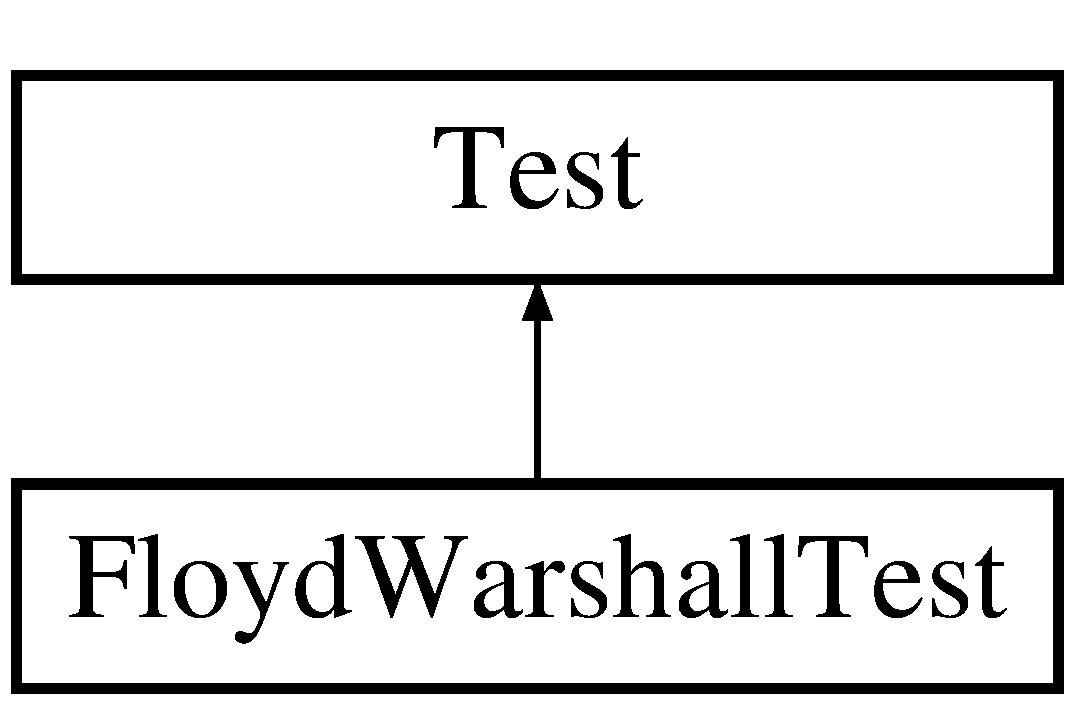
\includegraphics[height=2.000000cm]{class_floyd_warshall_test}
\end{center}
\end{figure}
\subsection*{Public Types}
\begin{DoxyCompactItemize}
\item 
typedef \hyperlink{struct_introduction_to_algorithm_1_1_graph_algorithm_1_1_graph}{Graph}$<$ F\+W\+\_\+\+N, \hyperlink{struct_introduction_to_algorithm_1_1_graph_algorithm_1_1_vertex}{Vertex}$<$ int $>$ $>$ \hyperlink{class_floyd_warshall_test_a4a5605ca735a94fb6f556aed58c83551}{G\+Type}
\end{DoxyCompactItemize}
\subsection*{Protected Member Functions}
\begin{DoxyCompactItemize}
\item 
void \hyperlink{class_floyd_warshall_test_af9de5944653730e05650280fa124d7c6}{Set\+Up} ()
\item 
void \hyperlink{class_floyd_warshall_test_aa1c5bddcfc5bea6a9882b6a56b2ee37f}{Tear\+Down} ()
\end{DoxyCompactItemize}
\subsection*{Protected Attributes}
\begin{DoxyCompactItemize}
\item 
std\+::shared\+\_\+ptr$<$ \hyperlink{class_floyd_warshall_test_a4a5605ca735a94fb6f556aed58c83551}{G\+Type} $>$ \hyperlink{class_floyd_warshall_test_a040517767832bad0943c797e4ef2c5ab}{\+\_\+graph}
\end{DoxyCompactItemize}


\subsection{Detailed Description}
\hyperlink{class_floyd_warshall_test}{Floyd\+Warshall\+Test}\+:测试类,用于为测试提供基础数据 

{\ttfamily \hyperlink{class_floyd_warshall_test}{Floyd\+Warshall\+Test}}是 {\ttfamily \+::testing\+::\+Test} 的子类。它主要用于为每一个{\ttfamily T\+E\+S\+T\+\_\+\+F}准备测试环境 

Definition at line 40 of file floyd\+\_\+warshall\+\_\+test.\+h.



\subsection{Member Typedef Documentation}
\hypertarget{class_floyd_warshall_test_a4a5605ca735a94fb6f556aed58c83551}{}\index{Floyd\+Warshall\+Test@{Floyd\+Warshall\+Test}!G\+Type@{G\+Type}}
\index{G\+Type@{G\+Type}!Floyd\+Warshall\+Test@{Floyd\+Warshall\+Test}}
\subsubsection[{G\+Type}]{\setlength{\rightskip}{0pt plus 5cm}typedef {\bf Graph}$<$F\+W\+\_\+\+N,{\bf Vertex}$<$int$>$ $>$ {\bf Floyd\+Warshall\+Test\+::\+G\+Type}}\label{class_floyd_warshall_test_a4a5605ca735a94fb6f556aed58c83551}
模板实例化的图类型,该图的顶点类型为{\ttfamily Vertex$<$int$>$} 

Definition at line 43 of file floyd\+\_\+warshall\+\_\+test.\+h.



\subsection{Member Function Documentation}
\hypertarget{class_floyd_warshall_test_af9de5944653730e05650280fa124d7c6}{}\index{Floyd\+Warshall\+Test@{Floyd\+Warshall\+Test}!Set\+Up@{Set\+Up}}
\index{Set\+Up@{Set\+Up}!Floyd\+Warshall\+Test@{Floyd\+Warshall\+Test}}
\subsubsection[{Set\+Up()}]{\setlength{\rightskip}{0pt plus 5cm}void Floyd\+Warshall\+Test\+::\+Set\+Up (
\begin{DoxyParamCaption}
{}
\end{DoxyParamCaption}
)\hspace{0.3cm}{\ttfamily [inline]}, {\ttfamily [protected]}}\label{class_floyd_warshall_test_af9de5944653730e05650280fa124d7c6}


Definition at line 46 of file floyd\+\_\+warshall\+\_\+test.\+h.

\hypertarget{class_floyd_warshall_test_aa1c5bddcfc5bea6a9882b6a56b2ee37f}{}\index{Floyd\+Warshall\+Test@{Floyd\+Warshall\+Test}!Tear\+Down@{Tear\+Down}}
\index{Tear\+Down@{Tear\+Down}!Floyd\+Warshall\+Test@{Floyd\+Warshall\+Test}}
\subsubsection[{Tear\+Down()}]{\setlength{\rightskip}{0pt plus 5cm}void Floyd\+Warshall\+Test\+::\+Tear\+Down (
\begin{DoxyParamCaption}
{}
\end{DoxyParamCaption}
)\hspace{0.3cm}{\ttfamily [inline]}, {\ttfamily [protected]}}\label{class_floyd_warshall_test_aa1c5bddcfc5bea6a9882b6a56b2ee37f}


Definition at line 64 of file floyd\+\_\+warshall\+\_\+test.\+h.



\subsection{Member Data Documentation}
\hypertarget{class_floyd_warshall_test_a040517767832bad0943c797e4ef2c5ab}{}\index{Floyd\+Warshall\+Test@{Floyd\+Warshall\+Test}!\+\_\+graph@{\+\_\+graph}}
\index{\+\_\+graph@{\+\_\+graph}!Floyd\+Warshall\+Test@{Floyd\+Warshall\+Test}}
\subsubsection[{\+\_\+graph}]{\setlength{\rightskip}{0pt plus 5cm}std\+::shared\+\_\+ptr$<${\bf G\+Type}$>$ Floyd\+Warshall\+Test\+::\+\_\+graph\hspace{0.3cm}{\ttfamily [protected]}}\label{class_floyd_warshall_test_a040517767832bad0943c797e4ef2c5ab}
指向一个图,算法导论图25-\/1 

Definition at line 65 of file floyd\+\_\+warshall\+\_\+test.\+h.



The documentation for this class was generated from the following file\+:\begin{DoxyCompactItemize}
\item 
src/graph\+\_\+algorithms/all\+\_\+node\+\_\+pair\+\_\+shortest\+\_\+path/floyd\+\_\+warshall/\hyperlink{floyd__warshall__test_8h}{floyd\+\_\+warshall\+\_\+test.\+h}\end{DoxyCompactItemize}

\hypertarget{class_ford_fulkerson_test}{}\section{Ford\+Fulkerson\+Test Class Reference}
\label{class_ford_fulkerson_test}\index{Ford\+Fulkerson\+Test@{Ford\+Fulkerson\+Test}}


\hyperlink{class_ford_fulkerson_test}{Ford\+Fulkerson\+Test}\+:测试类,用于为测试提供基础数据  




{\ttfamily \#include $<$fordfulkerson\+\_\+test.\+h$>$}

Inheritance diagram for Ford\+Fulkerson\+Test\+:\begin{figure}[H]
\begin{center}
\leavevmode
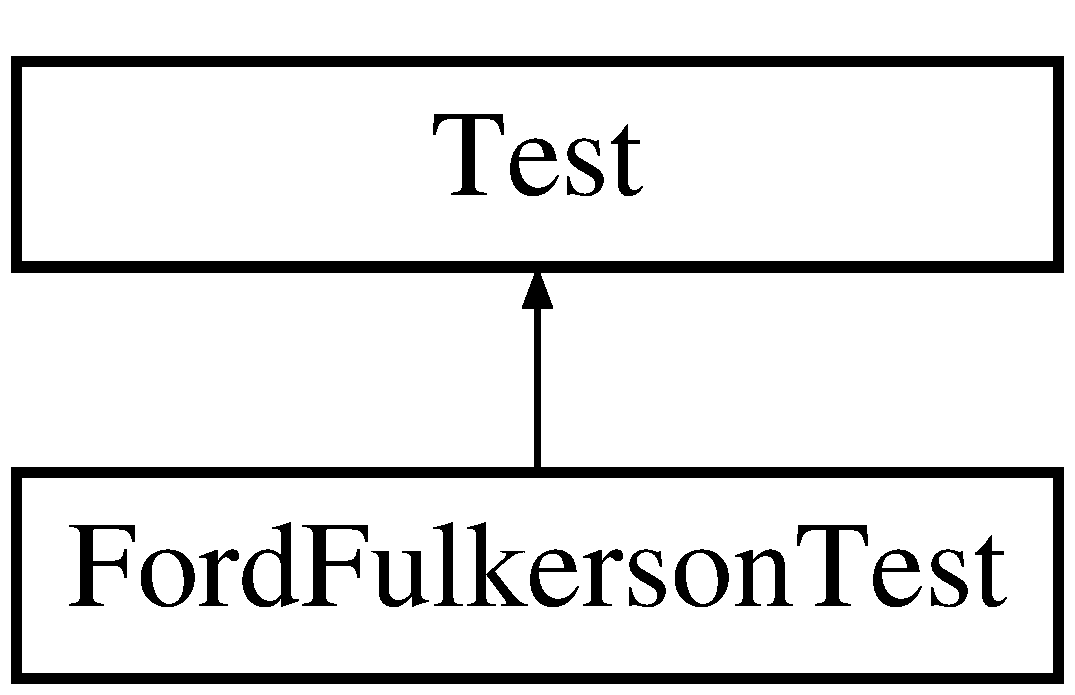
\includegraphics[height=2.000000cm]{class_ford_fulkerson_test}
\end{center}
\end{figure}
\subsection*{Public Types}
\begin{DoxyCompactItemize}
\item 
typedef \hyperlink{struct_introduction_to_algorithm_1_1_graph_algorithm_1_1_graph}{Graph}$<$ F\+F\+\_\+\+N, \hyperlink{struct_introduction_to_algorithm_1_1_graph_algorithm_1_1_b_f_s___vertex}{B\+F\+S\+\_\+\+Vertex}$<$ int $>$ $>$ \hyperlink{class_ford_fulkerson_test_a58e2f6af86c26eced9f7b316c5fa5d88}{G\+Type}
\end{DoxyCompactItemize}
\subsection*{Protected Member Functions}
\begin{DoxyCompactItemize}
\item 
void \hyperlink{class_ford_fulkerson_test_af70f0b88d1d16cd50c76df0f98f706b0}{Set\+Up} ()
\item 
void \hyperlink{class_ford_fulkerson_test_afcbc3160890661b9ae6d18a3a15bf6a6}{Tear\+Down} ()
\end{DoxyCompactItemize}
\subsection*{Protected Attributes}
\begin{DoxyCompactItemize}
\item 
std\+::shared\+\_\+ptr$<$ \hyperlink{class_ford_fulkerson_test_a58e2f6af86c26eced9f7b316c5fa5d88}{G\+Type} $>$ \hyperlink{class_ford_fulkerson_test_a4c5c58e3ebc1d2d324c67a8a9afe19e3}{\+\_\+graph}
\end{DoxyCompactItemize}


\subsection{Detailed Description}
\hyperlink{class_ford_fulkerson_test}{Ford\+Fulkerson\+Test}\+:测试类,用于为测试提供基础数据 

{\ttfamily \hyperlink{class_ford_fulkerson_test}{Ford\+Fulkerson\+Test}}是 {\ttfamily \+::testing\+::\+Test} 的子类。它主要用于为每一个{\ttfamily T\+E\+S\+T\+\_\+\+F}准备测试环境 

Definition at line 39 of file fordfulkerson\+\_\+test.\+h.



\subsection{Member Typedef Documentation}
\hypertarget{class_ford_fulkerson_test_a58e2f6af86c26eced9f7b316c5fa5d88}{}\index{Ford\+Fulkerson\+Test@{Ford\+Fulkerson\+Test}!G\+Type@{G\+Type}}
\index{G\+Type@{G\+Type}!Ford\+Fulkerson\+Test@{Ford\+Fulkerson\+Test}}
\subsubsection[{G\+Type}]{\setlength{\rightskip}{0pt plus 5cm}typedef {\bf Graph}$<$F\+F\+\_\+\+N,{\bf B\+F\+S\+\_\+\+Vertex}$<$int$>$ $>$ {\bf Ford\+Fulkerson\+Test\+::\+G\+Type}}\label{class_ford_fulkerson_test_a58e2f6af86c26eced9f7b316c5fa5d88}
模板实例化的图类型,该图的顶点类型为{\ttfamily B\+F\+S\+\_\+\+Vertex$<$int$>$} 

Definition at line 42 of file fordfulkerson\+\_\+test.\+h.



\subsection{Member Function Documentation}
\hypertarget{class_ford_fulkerson_test_af70f0b88d1d16cd50c76df0f98f706b0}{}\index{Ford\+Fulkerson\+Test@{Ford\+Fulkerson\+Test}!Set\+Up@{Set\+Up}}
\index{Set\+Up@{Set\+Up}!Ford\+Fulkerson\+Test@{Ford\+Fulkerson\+Test}}
\subsubsection[{Set\+Up()}]{\setlength{\rightskip}{0pt plus 5cm}void Ford\+Fulkerson\+Test\+::\+Set\+Up (
\begin{DoxyParamCaption}
{}
\end{DoxyParamCaption}
)\hspace{0.3cm}{\ttfamily [inline]}, {\ttfamily [protected]}}\label{class_ford_fulkerson_test_af70f0b88d1d16cd50c76df0f98f706b0}


Definition at line 45 of file fordfulkerson\+\_\+test.\+h.

\hypertarget{class_ford_fulkerson_test_afcbc3160890661b9ae6d18a3a15bf6a6}{}\index{Ford\+Fulkerson\+Test@{Ford\+Fulkerson\+Test}!Tear\+Down@{Tear\+Down}}
\index{Tear\+Down@{Tear\+Down}!Ford\+Fulkerson\+Test@{Ford\+Fulkerson\+Test}}
\subsubsection[{Tear\+Down()}]{\setlength{\rightskip}{0pt plus 5cm}void Ford\+Fulkerson\+Test\+::\+Tear\+Down (
\begin{DoxyParamCaption}
{}
\end{DoxyParamCaption}
)\hspace{0.3cm}{\ttfamily [inline]}, {\ttfamily [protected]}}\label{class_ford_fulkerson_test_afcbc3160890661b9ae6d18a3a15bf6a6}


Definition at line 63 of file fordfulkerson\+\_\+test.\+h.



\subsection{Member Data Documentation}
\hypertarget{class_ford_fulkerson_test_a4c5c58e3ebc1d2d324c67a8a9afe19e3}{}\index{Ford\+Fulkerson\+Test@{Ford\+Fulkerson\+Test}!\+\_\+graph@{\+\_\+graph}}
\index{\+\_\+graph@{\+\_\+graph}!Ford\+Fulkerson\+Test@{Ford\+Fulkerson\+Test}}
\subsubsection[{\+\_\+graph}]{\setlength{\rightskip}{0pt plus 5cm}std\+::shared\+\_\+ptr$<${\bf G\+Type}$>$ Ford\+Fulkerson\+Test\+::\+\_\+graph\hspace{0.3cm}{\ttfamily [protected]}}\label{class_ford_fulkerson_test_a4c5c58e3ebc1d2d324c67a8a9afe19e3}
指向一个图,算法导论图26-\/6 

Definition at line 64 of file fordfulkerson\+\_\+test.\+h.



The documentation for this class was generated from the following file\+:\begin{DoxyCompactItemize}
\item 
src/graph\+\_\+algorithms/max\+\_\+flow/ford\+\_\+fulkerson/\hyperlink{fordfulkerson__test_8h}{fordfulkerson\+\_\+test.\+h}\end{DoxyCompactItemize}

\hypertarget{struct_introduction_to_algorithm_1_1_graph_algorithm_1_1_front_flow_vertex}{}\section{Introduction\+To\+Algorithm\+:\+:Graph\+Algorithm\+:\+:Front\+Flow\+Vertex$<$ K\+Type $>$ Struct Template Reference}
\label{struct_introduction_to_algorithm_1_1_graph_algorithm_1_1_front_flow_vertex}\index{Introduction\+To\+Algorithm\+::\+Graph\+Algorithm\+::\+Front\+Flow\+Vertex$<$ K\+Type $>$@{Introduction\+To\+Algorithm\+::\+Graph\+Algorithm\+::\+Front\+Flow\+Vertex$<$ K\+Type $>$}}


Front\+Flow\+Vertex:relabel\+\_\+to\+\_\+front算法的图的结点的数据结构,算法导论26章26.4节  




{\ttfamily \#include $<$front\+\_\+flow\+\_\+vertex.\+h$>$}

Inheritance diagram for Introduction\+To\+Algorithm\+:\+:Graph\+Algorithm\+:\+:Front\+Flow\+Vertex$<$ K\+Type $>$\+:\begin{figure}[H]
\begin{center}
\leavevmode
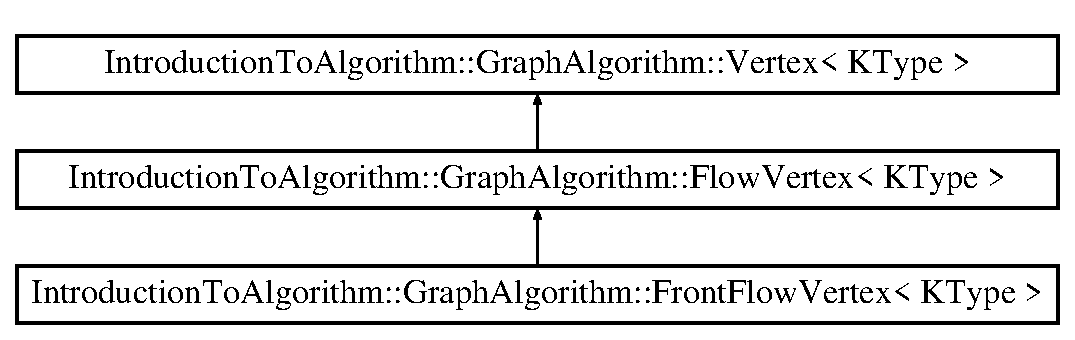
\includegraphics[height=3.000000cm]{struct_introduction_to_algorithm_1_1_graph_algorithm_1_1_front_flow_vertex}
\end{center}
\end{figure}
\subsection*{Public Types}
\begin{DoxyCompactItemize}
\item 
typedef K\+Type \hyperlink{struct_introduction_to_algorithm_1_1_graph_algorithm_1_1_front_flow_vertex_a76ed9e9d0c0da5c60c4a004eeda192ad}{Key\+Type}
\item 
typedef int \hyperlink{struct_introduction_to_algorithm_1_1_graph_algorithm_1_1_front_flow_vertex_ab1973e8ed99c2e213532fabbee1a66b8}{V\+I\+D\+Type}
\end{DoxyCompactItemize}
\subsection*{Public Member Functions}
\begin{DoxyCompactItemize}
\item 
\hyperlink{struct_introduction_to_algorithm_1_1_graph_algorithm_1_1_front_flow_vertex_a9890efaa1818c914f138ac063b679fe2}{Front\+Flow\+Vertex} ()
\begin{DoxyCompactList}\small\item\em 默认构造函数 \end{DoxyCompactList}\item 
\hyperlink{struct_introduction_to_algorithm_1_1_graph_algorithm_1_1_front_flow_vertex_af6c0dd18f309fdc4f6cd475a3f629f70}{Front\+Flow\+Vertex} (const \hyperlink{struct_introduction_to_algorithm_1_1_graph_algorithm_1_1_flow_vertex_a014b25c20124a24525ef7db0588466b9}{Key\+Type} \&k)
\begin{DoxyCompactList}\small\item\em 显式构造函数,指定{\ttfamily key} \end{DoxyCompactList}\item 
\hyperlink{struct_introduction_to_algorithm_1_1_graph_algorithm_1_1_front_flow_vertex_ae9af6850fbdfa4c8a192ea66778e6b59}{Front\+Flow\+Vertex} (const \hyperlink{struct_introduction_to_algorithm_1_1_graph_algorithm_1_1_flow_vertex_a014b25c20124a24525ef7db0588466b9}{Key\+Type} \&k, \hyperlink{struct_introduction_to_algorithm_1_1_graph_algorithm_1_1_flow_vertex_ae48ab0918590bd6a6763d007694ff161}{V\+I\+D\+Type} d)
\begin{DoxyCompactList}\small\item\em 显式构造函数,指定{\ttfamily key}和编号 \end{DoxyCompactList}\item 
virtual std\+::string \hyperlink{struct_introduction_to_algorithm_1_1_graph_algorithm_1_1_front_flow_vertex_a3edfb3a6f29475f338340291ad71eab9}{to\+\_\+string} () const 
\begin{DoxyCompactList}\small\item\em to\+\_\+string:返回顶点的字符串描述 \end{DoxyCompactList}\end{DoxyCompactItemize}
\subsection*{Public Attributes}
\begin{DoxyCompactItemize}
\item 
\hyperlink{struct_introduction_to_algorithm_1_1_graph_algorithm_1_1_list}{List}$<$ \hyperlink{struct_introduction_to_algorithm_1_1_graph_algorithm_1_1_list_node}{List\+Node}$<$ \hyperlink{struct_introduction_to_algorithm_1_1_graph_algorithm_1_1_front_flow_vertex}{Front\+Flow\+Vertex} $>$ $>$ \hyperlink{struct_introduction_to_algorithm_1_1_graph_algorithm_1_1_front_flow_vertex_ad66fead451e2af4756f0fd7a644e1319}{N\+\_\+\+List}
\end{DoxyCompactItemize}


\subsection{Detailed Description}
\subsubsection*{template$<$typename K\+Type$>$struct Introduction\+To\+Algorithm\+::\+Graph\+Algorithm\+::\+Front\+Flow\+Vertex$<$ K\+Type $>$}

Front\+Flow\+Vertex:relabel\+\_\+to\+\_\+front算法的图的结点的数据结构,算法导论26章26.4节 

\hyperlink{struct_introduction_to_algorithm_1_1_graph_algorithm_1_1_front_flow_vertex}{Front\+Flow\+Vertex} 继承自 Flow\+Vertex,它比\+Flow\+Vertex顶点多了一个{\ttfamily N\+\_\+\+List}数据成员,表示邻接链表

relabel\+\_\+to\+\_\+front 算法中,每一个\+Front\+Flow\+Vertex顶点位于两个级别的链表中:


\begin{DoxyItemize}
\item L 链表:最顶层的链表,\+L包含了所有的非源、非汇顶点
\item u.\+N 链表:某个顶点u的邻接链表 
\end{DoxyItemize}

Definition at line 175 of file front\+\_\+flow\+\_\+vertex.\+h.



\subsection{Member Typedef Documentation}
\hypertarget{struct_introduction_to_algorithm_1_1_graph_algorithm_1_1_front_flow_vertex_a76ed9e9d0c0da5c60c4a004eeda192ad}{}\index{Introduction\+To\+Algorithm\+::\+Graph\+Algorithm\+::\+Front\+Flow\+Vertex@{Introduction\+To\+Algorithm\+::\+Graph\+Algorithm\+::\+Front\+Flow\+Vertex}!Key\+Type@{Key\+Type}}
\index{Key\+Type@{Key\+Type}!Introduction\+To\+Algorithm\+::\+Graph\+Algorithm\+::\+Front\+Flow\+Vertex@{Introduction\+To\+Algorithm\+::\+Graph\+Algorithm\+::\+Front\+Flow\+Vertex}}
\subsubsection[{Key\+Type}]{\setlength{\rightskip}{0pt plus 5cm}template$<$typename K\+Type $>$ typedef K\+Type {\bf Introduction\+To\+Algorithm\+::\+Graph\+Algorithm\+::\+Front\+Flow\+Vertex}$<$ K\+Type $>$\+::{\bf Key\+Type}}\label{struct_introduction_to_algorithm_1_1_graph_algorithm_1_1_front_flow_vertex_a76ed9e9d0c0da5c60c4a004eeda192ad}
顶点存储数据的类型 

Definition at line 177 of file front\+\_\+flow\+\_\+vertex.\+h.

\hypertarget{struct_introduction_to_algorithm_1_1_graph_algorithm_1_1_front_flow_vertex_ab1973e8ed99c2e213532fabbee1a66b8}{}\index{Introduction\+To\+Algorithm\+::\+Graph\+Algorithm\+::\+Front\+Flow\+Vertex@{Introduction\+To\+Algorithm\+::\+Graph\+Algorithm\+::\+Front\+Flow\+Vertex}!V\+I\+D\+Type@{V\+I\+D\+Type}}
\index{V\+I\+D\+Type@{V\+I\+D\+Type}!Introduction\+To\+Algorithm\+::\+Graph\+Algorithm\+::\+Front\+Flow\+Vertex@{Introduction\+To\+Algorithm\+::\+Graph\+Algorithm\+::\+Front\+Flow\+Vertex}}
\subsubsection[{V\+I\+D\+Type}]{\setlength{\rightskip}{0pt plus 5cm}template$<$typename K\+Type $>$ typedef int {\bf Introduction\+To\+Algorithm\+::\+Graph\+Algorithm\+::\+Front\+Flow\+Vertex}$<$ K\+Type $>$\+::{\bf V\+I\+D\+Type}}\label{struct_introduction_to_algorithm_1_1_graph_algorithm_1_1_front_flow_vertex_ab1973e8ed99c2e213532fabbee1a66b8}
顶点编号的数据类型 

Definition at line 178 of file front\+\_\+flow\+\_\+vertex.\+h.



\subsection{Constructor \& Destructor Documentation}
\hypertarget{struct_introduction_to_algorithm_1_1_graph_algorithm_1_1_front_flow_vertex_a9890efaa1818c914f138ac063b679fe2}{}\index{Introduction\+To\+Algorithm\+::\+Graph\+Algorithm\+::\+Front\+Flow\+Vertex@{Introduction\+To\+Algorithm\+::\+Graph\+Algorithm\+::\+Front\+Flow\+Vertex}!Front\+Flow\+Vertex@{Front\+Flow\+Vertex}}
\index{Front\+Flow\+Vertex@{Front\+Flow\+Vertex}!Introduction\+To\+Algorithm\+::\+Graph\+Algorithm\+::\+Front\+Flow\+Vertex@{Introduction\+To\+Algorithm\+::\+Graph\+Algorithm\+::\+Front\+Flow\+Vertex}}
\subsubsection[{Front\+Flow\+Vertex()}]{\setlength{\rightskip}{0pt plus 5cm}template$<$typename K\+Type $>$ {\bf Introduction\+To\+Algorithm\+::\+Graph\+Algorithm\+::\+Front\+Flow\+Vertex}$<$ K\+Type $>$\+::{\bf Front\+Flow\+Vertex} (
\begin{DoxyParamCaption}
{}
\end{DoxyParamCaption}
)\hspace{0.3cm}{\ttfamily [inline]}}\label{struct_introduction_to_algorithm_1_1_graph_algorithm_1_1_front_flow_vertex_a9890efaa1818c914f138ac063b679fe2}


默认构造函数 



Definition at line 183 of file front\+\_\+flow\+\_\+vertex.\+h.

\hypertarget{struct_introduction_to_algorithm_1_1_graph_algorithm_1_1_front_flow_vertex_af6c0dd18f309fdc4f6cd475a3f629f70}{}\index{Introduction\+To\+Algorithm\+::\+Graph\+Algorithm\+::\+Front\+Flow\+Vertex@{Introduction\+To\+Algorithm\+::\+Graph\+Algorithm\+::\+Front\+Flow\+Vertex}!Front\+Flow\+Vertex@{Front\+Flow\+Vertex}}
\index{Front\+Flow\+Vertex@{Front\+Flow\+Vertex}!Introduction\+To\+Algorithm\+::\+Graph\+Algorithm\+::\+Front\+Flow\+Vertex@{Introduction\+To\+Algorithm\+::\+Graph\+Algorithm\+::\+Front\+Flow\+Vertex}}
\subsubsection[{Front\+Flow\+Vertex(const Key\+Type \&k)}]{\setlength{\rightskip}{0pt plus 5cm}template$<$typename K\+Type $>$ {\bf Introduction\+To\+Algorithm\+::\+Graph\+Algorithm\+::\+Front\+Flow\+Vertex}$<$ K\+Type $>$\+::{\bf Front\+Flow\+Vertex} (
\begin{DoxyParamCaption}
\item[{const {\bf Key\+Type} \&}]{k}
\end{DoxyParamCaption}
)\hspace{0.3cm}{\ttfamily [inline]}, {\ttfamily [explicit]}}\label{struct_introduction_to_algorithm_1_1_graph_algorithm_1_1_front_flow_vertex_af6c0dd18f309fdc4f6cd475a3f629f70}


显式构造函数,指定{\ttfamily key} 


\begin{DoxyParams}{Parameters}
{\em k\+:顶点存放的数据} & \\
\hline
\end{DoxyParams}


Definition at line 188 of file front\+\_\+flow\+\_\+vertex.\+h.

\hypertarget{struct_introduction_to_algorithm_1_1_graph_algorithm_1_1_front_flow_vertex_ae9af6850fbdfa4c8a192ea66778e6b59}{}\index{Introduction\+To\+Algorithm\+::\+Graph\+Algorithm\+::\+Front\+Flow\+Vertex@{Introduction\+To\+Algorithm\+::\+Graph\+Algorithm\+::\+Front\+Flow\+Vertex}!Front\+Flow\+Vertex@{Front\+Flow\+Vertex}}
\index{Front\+Flow\+Vertex@{Front\+Flow\+Vertex}!Introduction\+To\+Algorithm\+::\+Graph\+Algorithm\+::\+Front\+Flow\+Vertex@{Introduction\+To\+Algorithm\+::\+Graph\+Algorithm\+::\+Front\+Flow\+Vertex}}
\subsubsection[{Front\+Flow\+Vertex(const Key\+Type \&k, V\+I\+D\+Type d)}]{\setlength{\rightskip}{0pt plus 5cm}template$<$typename K\+Type $>$ {\bf Introduction\+To\+Algorithm\+::\+Graph\+Algorithm\+::\+Front\+Flow\+Vertex}$<$ K\+Type $>$\+::{\bf Front\+Flow\+Vertex} (
\begin{DoxyParamCaption}
\item[{const {\bf Key\+Type} \&}]{k, }
\item[{{\bf V\+I\+D\+Type}}]{d}
\end{DoxyParamCaption}
)\hspace{0.3cm}{\ttfamily [inline]}}\label{struct_introduction_to_algorithm_1_1_graph_algorithm_1_1_front_flow_vertex_ae9af6850fbdfa4c8a192ea66778e6b59}


显式构造函数,指定{\ttfamily key}和编号 


\begin{DoxyParams}{Parameters}
{\em k\+:顶点存放的数据} & \\
\hline
{\em d\+:顶点的编号} & \\
\hline
\end{DoxyParams}


Definition at line 194 of file front\+\_\+flow\+\_\+vertex.\+h.



\subsection{Member Function Documentation}
\hypertarget{struct_introduction_to_algorithm_1_1_graph_algorithm_1_1_front_flow_vertex_a3edfb3a6f29475f338340291ad71eab9}{}\index{Introduction\+To\+Algorithm\+::\+Graph\+Algorithm\+::\+Front\+Flow\+Vertex@{Introduction\+To\+Algorithm\+::\+Graph\+Algorithm\+::\+Front\+Flow\+Vertex}!to\+\_\+string@{to\+\_\+string}}
\index{to\+\_\+string@{to\+\_\+string}!Introduction\+To\+Algorithm\+::\+Graph\+Algorithm\+::\+Front\+Flow\+Vertex@{Introduction\+To\+Algorithm\+::\+Graph\+Algorithm\+::\+Front\+Flow\+Vertex}}
\subsubsection[{to\+\_\+string() const }]{\setlength{\rightskip}{0pt plus 5cm}template$<$typename K\+Type $>$ virtual std\+::string {\bf Introduction\+To\+Algorithm\+::\+Graph\+Algorithm\+::\+Front\+Flow\+Vertex}$<$ K\+Type $>$\+::to\+\_\+string (
\begin{DoxyParamCaption}
{}
\end{DoxyParamCaption}
) const\hspace{0.3cm}{\ttfamily [inline]}, {\ttfamily [virtual]}}\label{struct_introduction_to_algorithm_1_1_graph_algorithm_1_1_front_flow_vertex_a3edfb3a6f29475f338340291ad71eab9}


to\+\_\+string:返回顶点的字符串描述 

\begin{DoxyReturn}{Returns}
\+:顶点的字符串描述
\end{DoxyReturn}
在{\ttfamily \hyperlink{struct_introduction_to_algorithm_1_1_graph_algorithm_1_1_flow_vertex}{Flow\+Vertex}}基类的基础上输出{\ttfamily N\+\_\+\+List}信息 

Reimplemented from \hyperlink{struct_introduction_to_algorithm_1_1_graph_algorithm_1_1_flow_vertex_aa373a13a1fdee1fdcdbd0b55eaa1d1fb}{Introduction\+To\+Algorithm\+::\+Graph\+Algorithm\+::\+Flow\+Vertex$<$ K\+Type $>$}.



Definition at line 202 of file front\+\_\+flow\+\_\+vertex.\+h.



\subsection{Member Data Documentation}
\hypertarget{struct_introduction_to_algorithm_1_1_graph_algorithm_1_1_front_flow_vertex_ad66fead451e2af4756f0fd7a644e1319}{}\index{Introduction\+To\+Algorithm\+::\+Graph\+Algorithm\+::\+Front\+Flow\+Vertex@{Introduction\+To\+Algorithm\+::\+Graph\+Algorithm\+::\+Front\+Flow\+Vertex}!N\+\_\+\+List@{N\+\_\+\+List}}
\index{N\+\_\+\+List@{N\+\_\+\+List}!Introduction\+To\+Algorithm\+::\+Graph\+Algorithm\+::\+Front\+Flow\+Vertex@{Introduction\+To\+Algorithm\+::\+Graph\+Algorithm\+::\+Front\+Flow\+Vertex}}
\subsubsection[{N\+\_\+\+List}]{\setlength{\rightskip}{0pt plus 5cm}template$<$typename K\+Type $>$ {\bf List}$<${\bf List\+Node}$<${\bf Front\+Flow\+Vertex}$>$ $>$ {\bf Introduction\+To\+Algorithm\+::\+Graph\+Algorithm\+::\+Front\+Flow\+Vertex}$<$ K\+Type $>$\+::N\+\_\+\+List}\label{struct_introduction_to_algorithm_1_1_graph_algorithm_1_1_front_flow_vertex_ad66fead451e2af4756f0fd7a644e1319}
顶点的邻接链表 

Definition at line 180 of file front\+\_\+flow\+\_\+vertex.\+h.



The documentation for this struct was generated from the following file\+:\begin{DoxyCompactItemize}
\item 
src/graph\+\_\+algorithms/basic\+\_\+graph/graph\+\_\+representation/graph\+\_\+vertex/\hyperlink{front__flow__vertex_8h}{front\+\_\+flow\+\_\+vertex.\+h}\end{DoxyCompactItemize}

\hypertarget{class_front_flow_vertex_test}{}\section{Front\+Flow\+Vertex\+Test Class Reference}
\label{class_front_flow_vertex_test}\index{Front\+Flow\+Vertex\+Test@{Front\+Flow\+Vertex\+Test}}


{\ttfamily \#include $<$front\+\_\+flow\+\_\+vertex\+\_\+test.\+h$>$}

Inheritance diagram for Front\+Flow\+Vertex\+Test\+:\begin{figure}[H]
\begin{center}
\leavevmode
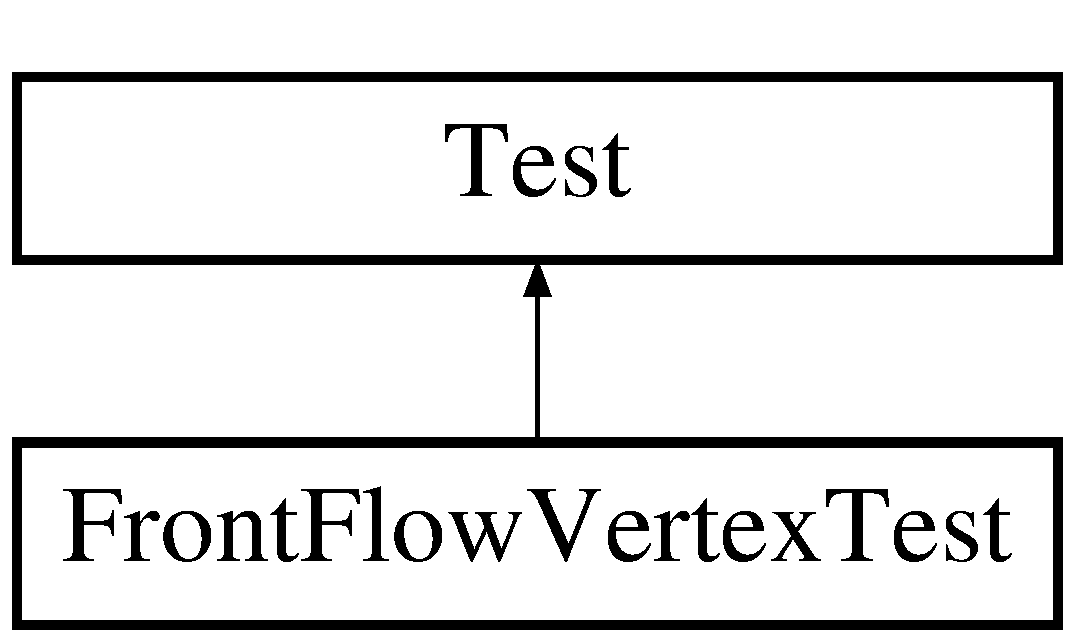
\includegraphics[height=2.000000cm]{class_front_flow_vertex_test}
\end{center}
\end{figure}
\subsection*{Public Types}
\begin{DoxyCompactItemize}
\item 
typedef \hyperlink{struct_introduction_to_algorithm_1_1_graph_algorithm_1_1_front_flow_vertex}{Front\+Flow\+Vertex}$<$ int $>$ \hyperlink{class_front_flow_vertex_test_a0eefc91d4672952fe46aafe55b41d195}{Vertex\+Type}
\item 
typedef \hyperlink{struct_introduction_to_algorithm_1_1_graph_algorithm_1_1_list_node}{List\+Node}$<$ \hyperlink{class_front_flow_vertex_test_a0eefc91d4672952fe46aafe55b41d195}{Vertex\+Type} $>$ \hyperlink{class_front_flow_vertex_test_a80f3e381f6911872f7a4359ceff966bf}{Node\+Type}
\item 
typedef \hyperlink{struct_introduction_to_algorithm_1_1_graph_algorithm_1_1_list}{List}$<$ \hyperlink{class_front_flow_vertex_test_a80f3e381f6911872f7a4359ceff966bf}{Node\+Type} $>$ \hyperlink{class_front_flow_vertex_test_ac30f272d98796ffce519f894f111fcaa}{List\+Type}
\end{DoxyCompactItemize}
\subsection*{Protected Member Functions}
\begin{DoxyCompactItemize}
\item 
void \hyperlink{class_front_flow_vertex_test_a8dfe07d5a92c681dcaa64ecc7dab5e2f}{Set\+Up} ()
\item 
void \hyperlink{class_front_flow_vertex_test_a653d242a450fdfd6eed74c6540154681}{Tear\+Down} ()
\end{DoxyCompactItemize}
\subsection*{Protected Attributes}
\begin{DoxyCompactItemize}
\item 
std\+::shared\+\_\+ptr$<$ \hyperlink{class_front_flow_vertex_test_a0eefc91d4672952fe46aafe55b41d195}{Vertex\+Type} $>$ \hyperlink{class_front_flow_vertex_test_a457ca07d1faf2d24e8bf7ab0116e822f}{\+\_\+default\+\_\+vertex}
\item 
std\+::shared\+\_\+ptr$<$ \hyperlink{class_front_flow_vertex_test_a0eefc91d4672952fe46aafe55b41d195}{Vertex\+Type} $>$ \hyperlink{class_front_flow_vertex_test_a5f8a63b2d218d2e733e27ca598e9b864}{\+\_\+normal\+\_\+vertex}
\item 
std\+::shared\+\_\+ptr$<$ \hyperlink{class_front_flow_vertex_test_ac30f272d98796ffce519f894f111fcaa}{List\+Type} $>$ \hyperlink{class_front_flow_vertex_test_a646ef544a16221c204d71d777c76b17b}{\+\_\+list}
\item 
std\+::shared\+\_\+ptr$<$ \hyperlink{class_front_flow_vertex_test_a80f3e381f6911872f7a4359ceff966bf}{Node\+Type} $>$ \hyperlink{class_front_flow_vertex_test_a87ecf1ffdaa2b7c78ba360b2deb4cfd1}{\+\_\+nodes} \mbox{[}F\+F\+V\+\_\+\+N\+U\+M\mbox{]}
\end{DoxyCompactItemize}


\subsection{Detailed Description}


Definition at line 30 of file front\+\_\+flow\+\_\+vertex\+\_\+test.\+h.



\subsection{Member Typedef Documentation}
\hypertarget{class_front_flow_vertex_test_ac30f272d98796ffce519f894f111fcaa}{}\index{Front\+Flow\+Vertex\+Test@{Front\+Flow\+Vertex\+Test}!List\+Type@{List\+Type}}
\index{List\+Type@{List\+Type}!Front\+Flow\+Vertex\+Test@{Front\+Flow\+Vertex\+Test}}
\subsubsection[{List\+Type}]{\setlength{\rightskip}{0pt plus 5cm}typedef {\bf List}$<${\bf Node\+Type}$>$ {\bf Front\+Flow\+Vertex\+Test\+::\+List\+Type}}\label{class_front_flow_vertex_test_ac30f272d98796ffce519f894f111fcaa}
模板实例化的链表类型 

Definition at line 35 of file front\+\_\+flow\+\_\+vertex\+\_\+test.\+h.

\hypertarget{class_front_flow_vertex_test_a80f3e381f6911872f7a4359ceff966bf}{}\index{Front\+Flow\+Vertex\+Test@{Front\+Flow\+Vertex\+Test}!Node\+Type@{Node\+Type}}
\index{Node\+Type@{Node\+Type}!Front\+Flow\+Vertex\+Test@{Front\+Flow\+Vertex\+Test}}
\subsubsection[{Node\+Type}]{\setlength{\rightskip}{0pt plus 5cm}typedef {\bf List\+Node}$<${\bf Vertex\+Type}$>$ {\bf Front\+Flow\+Vertex\+Test\+::\+Node\+Type}}\label{class_front_flow_vertex_test_a80f3e381f6911872f7a4359ceff966bf}
模板实例化的\+Node类型 

Definition at line 34 of file front\+\_\+flow\+\_\+vertex\+\_\+test.\+h.

\hypertarget{class_front_flow_vertex_test_a0eefc91d4672952fe46aafe55b41d195}{}\index{Front\+Flow\+Vertex\+Test@{Front\+Flow\+Vertex\+Test}!Vertex\+Type@{Vertex\+Type}}
\index{Vertex\+Type@{Vertex\+Type}!Front\+Flow\+Vertex\+Test@{Front\+Flow\+Vertex\+Test}}
\subsubsection[{Vertex\+Type}]{\setlength{\rightskip}{0pt plus 5cm}typedef {\bf Front\+Flow\+Vertex}$<$int$>$ {\bf Front\+Flow\+Vertex\+Test\+::\+Vertex\+Type}}\label{class_front_flow_vertex_test_a0eefc91d4672952fe46aafe55b41d195}
模板实例化的顶点类型 

Definition at line 33 of file front\+\_\+flow\+\_\+vertex\+\_\+test.\+h.



\subsection{Member Function Documentation}
\hypertarget{class_front_flow_vertex_test_a8dfe07d5a92c681dcaa64ecc7dab5e2f}{}\index{Front\+Flow\+Vertex\+Test@{Front\+Flow\+Vertex\+Test}!Set\+Up@{Set\+Up}}
\index{Set\+Up@{Set\+Up}!Front\+Flow\+Vertex\+Test@{Front\+Flow\+Vertex\+Test}}
\subsubsection[{Set\+Up()}]{\setlength{\rightskip}{0pt plus 5cm}void Front\+Flow\+Vertex\+Test\+::\+Set\+Up (
\begin{DoxyParamCaption}
{}
\end{DoxyParamCaption}
)\hspace{0.3cm}{\ttfamily [inline]}, {\ttfamily [protected]}}\label{class_front_flow_vertex_test_a8dfe07d5a92c681dcaa64ecc7dab5e2f}


Definition at line 38 of file front\+\_\+flow\+\_\+vertex\+\_\+test.\+h.

\hypertarget{class_front_flow_vertex_test_a653d242a450fdfd6eed74c6540154681}{}\index{Front\+Flow\+Vertex\+Test@{Front\+Flow\+Vertex\+Test}!Tear\+Down@{Tear\+Down}}
\index{Tear\+Down@{Tear\+Down}!Front\+Flow\+Vertex\+Test@{Front\+Flow\+Vertex\+Test}}
\subsubsection[{Tear\+Down()}]{\setlength{\rightskip}{0pt plus 5cm}void Front\+Flow\+Vertex\+Test\+::\+Tear\+Down (
\begin{DoxyParamCaption}
{}
\end{DoxyParamCaption}
)\hspace{0.3cm}{\ttfamily [inline]}, {\ttfamily [protected]}}\label{class_front_flow_vertex_test_a653d242a450fdfd6eed74c6540154681}


Definition at line 49 of file front\+\_\+flow\+\_\+vertex\+\_\+test.\+h.



\subsection{Member Data Documentation}
\hypertarget{class_front_flow_vertex_test_a457ca07d1faf2d24e8bf7ab0116e822f}{}\index{Front\+Flow\+Vertex\+Test@{Front\+Flow\+Vertex\+Test}!\+\_\+default\+\_\+vertex@{\+\_\+default\+\_\+vertex}}
\index{\+\_\+default\+\_\+vertex@{\+\_\+default\+\_\+vertex}!Front\+Flow\+Vertex\+Test@{Front\+Flow\+Vertex\+Test}}
\subsubsection[{\+\_\+default\+\_\+vertex}]{\setlength{\rightskip}{0pt plus 5cm}std\+::shared\+\_\+ptr$<${\bf Vertex\+Type}$>$ Front\+Flow\+Vertex\+Test\+::\+\_\+default\+\_\+vertex\hspace{0.3cm}{\ttfamily [protected]}}\label{class_front_flow_vertex_test_a457ca07d1faf2d24e8bf7ab0116e822f}
默认构造的顶点 

Definition at line 51 of file front\+\_\+flow\+\_\+vertex\+\_\+test.\+h.

\hypertarget{class_front_flow_vertex_test_a646ef544a16221c204d71d777c76b17b}{}\index{Front\+Flow\+Vertex\+Test@{Front\+Flow\+Vertex\+Test}!\+\_\+list@{\+\_\+list}}
\index{\+\_\+list@{\+\_\+list}!Front\+Flow\+Vertex\+Test@{Front\+Flow\+Vertex\+Test}}
\subsubsection[{\+\_\+list}]{\setlength{\rightskip}{0pt plus 5cm}std\+::shared\+\_\+ptr$<${\bf List\+Type}$>$ Front\+Flow\+Vertex\+Test\+::\+\_\+list\hspace{0.3cm}{\ttfamily [protected]}}\label{class_front_flow_vertex_test_a646ef544a16221c204d71d777c76b17b}
列表顶点 

Definition at line 54 of file front\+\_\+flow\+\_\+vertex\+\_\+test.\+h.

\hypertarget{class_front_flow_vertex_test_a87ecf1ffdaa2b7c78ba360b2deb4cfd1}{}\index{Front\+Flow\+Vertex\+Test@{Front\+Flow\+Vertex\+Test}!\+\_\+nodes@{\+\_\+nodes}}
\index{\+\_\+nodes@{\+\_\+nodes}!Front\+Flow\+Vertex\+Test@{Front\+Flow\+Vertex\+Test}}
\subsubsection[{\+\_\+nodes}]{\setlength{\rightskip}{0pt plus 5cm}std\+::shared\+\_\+ptr$<${\bf Node\+Type}$>$ Front\+Flow\+Vertex\+Test\+::\+\_\+nodes\mbox{[}F\+F\+V\+\_\+\+N\+U\+M\mbox{]}\hspace{0.3cm}{\ttfamily [protected]}}\label{class_front_flow_vertex_test_a87ecf1ffdaa2b7c78ba360b2deb4cfd1}
顶点 

Definition at line 55 of file front\+\_\+flow\+\_\+vertex\+\_\+test.\+h.

\hypertarget{class_front_flow_vertex_test_a5f8a63b2d218d2e733e27ca598e9b864}{}\index{Front\+Flow\+Vertex\+Test@{Front\+Flow\+Vertex\+Test}!\+\_\+normal\+\_\+vertex@{\+\_\+normal\+\_\+vertex}}
\index{\+\_\+normal\+\_\+vertex@{\+\_\+normal\+\_\+vertex}!Front\+Flow\+Vertex\+Test@{Front\+Flow\+Vertex\+Test}}
\subsubsection[{\+\_\+normal\+\_\+vertex}]{\setlength{\rightskip}{0pt plus 5cm}std\+::shared\+\_\+ptr$<${\bf Vertex\+Type}$>$ Front\+Flow\+Vertex\+Test\+::\+\_\+normal\+\_\+vertex\hspace{0.3cm}{\ttfamily [protected]}}\label{class_front_flow_vertex_test_a5f8a63b2d218d2e733e27ca598e9b864}
正常构造的顶点 

Definition at line 52 of file front\+\_\+flow\+\_\+vertex\+\_\+test.\+h.



The documentation for this class was generated from the following file\+:\begin{DoxyCompactItemize}
\item 
src/graph\+\_\+algorithms/basic\+\_\+graph/graph\+\_\+representation/graph\+\_\+vertex/\hyperlink{front__flow__vertex__test_8h}{front\+\_\+flow\+\_\+vertex\+\_\+test.\+h}\end{DoxyCompactItemize}

\hypertarget{class_generic_push_relabel_test}{}\section{Generic\+Push\+Relabel\+Test Class Reference}
\label{class_generic_push_relabel_test}\index{Generic\+Push\+Relabel\+Test@{Generic\+Push\+Relabel\+Test}}


\hyperlink{class_generic_push_relabel_test}{Generic\+Push\+Relabel\+Test}\+:测试类,用于为测试提供基础数据  




{\ttfamily \#include $<$genericpushrelabel\+\_\+test.\+h$>$}

Inheritance diagram for Generic\+Push\+Relabel\+Test\+:\begin{figure}[H]
\begin{center}
\leavevmode
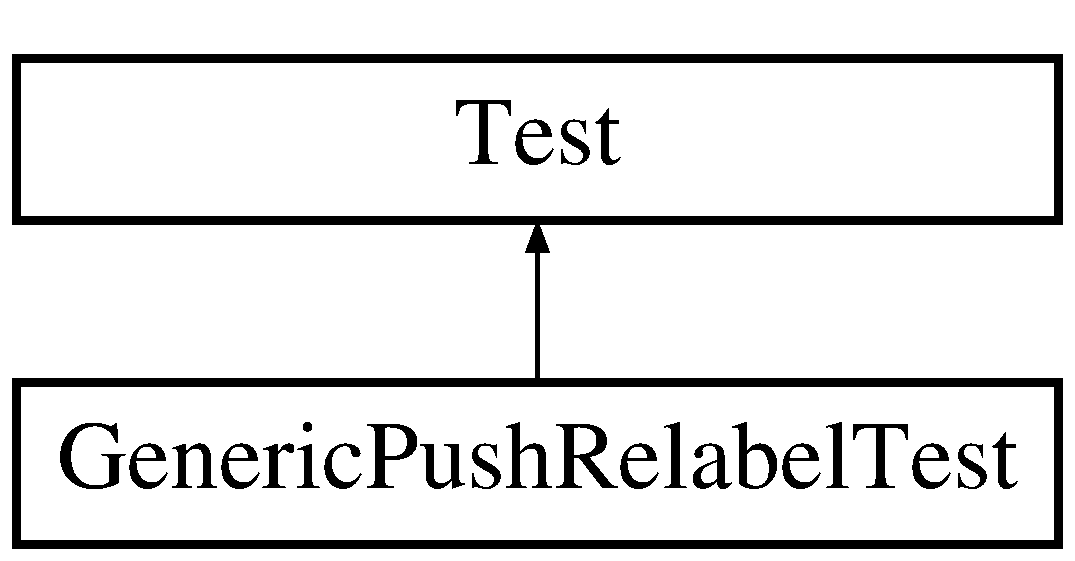
\includegraphics[height=2.000000cm]{class_generic_push_relabel_test}
\end{center}
\end{figure}
\subsection*{Public Types}
\begin{DoxyCompactItemize}
\item 
typedef \hyperlink{struct_introduction_to_algorithm_1_1_graph_algorithm_1_1_graph}{Graph}$<$ P\+R\+\_\+\+N, \hyperlink{struct_introduction_to_algorithm_1_1_graph_algorithm_1_1_flow_vertex}{Flow\+Vertex}$<$ int $>$ $>$ \hyperlink{class_generic_push_relabel_test_af6684144e5419944b2fe025117401bbc}{G\+Type}
\end{DoxyCompactItemize}
\subsection*{Protected Member Functions}
\begin{DoxyCompactItemize}
\item 
void \hyperlink{class_generic_push_relabel_test_ad6fe14069d4f8edf4718c55f23b2e0d8}{Set\+Up} ()
\item 
void \hyperlink{class_generic_push_relabel_test_a90c573a2500d5dda0243d429a606aa6b}{Tear\+Down} ()
\end{DoxyCompactItemize}
\subsection*{Protected Attributes}
\begin{DoxyCompactItemize}
\item 
std\+::shared\+\_\+ptr$<$ \hyperlink{class_generic_push_relabel_test_af6684144e5419944b2fe025117401bbc}{G\+Type} $>$ \hyperlink{class_generic_push_relabel_test_aa363ed3e48e55d7f5451797f3432554c}{\+\_\+graph}
\end{DoxyCompactItemize}


\subsection{Detailed Description}
\hyperlink{class_generic_push_relabel_test}{Generic\+Push\+Relabel\+Test}\+:测试类,用于为测试提供基础数据 

{\ttfamily \hyperlink{class_generic_push_relabel_test}{Generic\+Push\+Relabel\+Test}}是 {\ttfamily \+::testing\+::\+Test} 的子类。它主要用于为每一个{\ttfamily T\+E\+S\+T\+\_\+\+F}准备测试环境 

Definition at line 43 of file genericpushrelabel\+\_\+test.\+h.



\subsection{Member Typedef Documentation}
\hypertarget{class_generic_push_relabel_test_af6684144e5419944b2fe025117401bbc}{}\index{Generic\+Push\+Relabel\+Test@{Generic\+Push\+Relabel\+Test}!G\+Type@{G\+Type}}
\index{G\+Type@{G\+Type}!Generic\+Push\+Relabel\+Test@{Generic\+Push\+Relabel\+Test}}
\subsubsection[{G\+Type}]{\setlength{\rightskip}{0pt plus 5cm}typedef {\bf Graph}$<$P\+R\+\_\+\+N,{\bf Flow\+Vertex}$<$int$>$ $>$ {\bf Generic\+Push\+Relabel\+Test\+::\+G\+Type}}\label{class_generic_push_relabel_test_af6684144e5419944b2fe025117401bbc}
模板实例化的图类型,该图的顶点类型为{\ttfamily Flow\+Vertex$<$int$>$} 

Definition at line 46 of file genericpushrelabel\+\_\+test.\+h.



\subsection{Member Function Documentation}
\hypertarget{class_generic_push_relabel_test_ad6fe14069d4f8edf4718c55f23b2e0d8}{}\index{Generic\+Push\+Relabel\+Test@{Generic\+Push\+Relabel\+Test}!Set\+Up@{Set\+Up}}
\index{Set\+Up@{Set\+Up}!Generic\+Push\+Relabel\+Test@{Generic\+Push\+Relabel\+Test}}
\subsubsection[{Set\+Up()}]{\setlength{\rightskip}{0pt plus 5cm}void Generic\+Push\+Relabel\+Test\+::\+Set\+Up (
\begin{DoxyParamCaption}
{}
\end{DoxyParamCaption}
)\hspace{0.3cm}{\ttfamily [inline]}, {\ttfamily [protected]}}\label{class_generic_push_relabel_test_ad6fe14069d4f8edf4718c55f23b2e0d8}


Definition at line 49 of file genericpushrelabel\+\_\+test.\+h.

\hypertarget{class_generic_push_relabel_test_a90c573a2500d5dda0243d429a606aa6b}{}\index{Generic\+Push\+Relabel\+Test@{Generic\+Push\+Relabel\+Test}!Tear\+Down@{Tear\+Down}}
\index{Tear\+Down@{Tear\+Down}!Generic\+Push\+Relabel\+Test@{Generic\+Push\+Relabel\+Test}}
\subsubsection[{Tear\+Down()}]{\setlength{\rightskip}{0pt plus 5cm}void Generic\+Push\+Relabel\+Test\+::\+Tear\+Down (
\begin{DoxyParamCaption}
{}
\end{DoxyParamCaption}
)\hspace{0.3cm}{\ttfamily [inline]}, {\ttfamily [protected]}}\label{class_generic_push_relabel_test_a90c573a2500d5dda0243d429a606aa6b}


Definition at line 67 of file genericpushrelabel\+\_\+test.\+h.



\subsection{Member Data Documentation}
\hypertarget{class_generic_push_relabel_test_aa363ed3e48e55d7f5451797f3432554c}{}\index{Generic\+Push\+Relabel\+Test@{Generic\+Push\+Relabel\+Test}!\+\_\+graph@{\+\_\+graph}}
\index{\+\_\+graph@{\+\_\+graph}!Generic\+Push\+Relabel\+Test@{Generic\+Push\+Relabel\+Test}}
\subsubsection[{\+\_\+graph}]{\setlength{\rightskip}{0pt plus 5cm}std\+::shared\+\_\+ptr$<${\bf G\+Type}$>$ Generic\+Push\+Relabel\+Test\+::\+\_\+graph\hspace{0.3cm}{\ttfamily [protected]}}\label{class_generic_push_relabel_test_aa363ed3e48e55d7f5451797f3432554c}
指向一个图,算法导论图26-\/6 

Definition at line 68 of file genericpushrelabel\+\_\+test.\+h.



The documentation for this class was generated from the following file\+:\begin{DoxyCompactItemize}
\item 
src/graph\+\_\+algorithms/max\+\_\+flow/generic\+\_\+push\+\_\+relabel/\hyperlink{genericpushrelabel__test_8h}{genericpushrelabel\+\_\+test.\+h}\end{DoxyCompactItemize}

\hypertarget{struct_introduction_to_algorithm_1_1_graph_algorithm_1_1_graph}{}\section{Introduction\+To\+Algorithm\+:\+:Graph\+Algorithm\+:\+:Graph$<$ N, V\+Type $>$ Struct Template Reference}
\label{struct_introduction_to_algorithm_1_1_graph_algorithm_1_1_graph}\index{Introduction\+To\+Algorithm\+::\+Graph\+Algorithm\+::\+Graph$<$ N, V\+Type $>$@{Introduction\+To\+Algorithm\+::\+Graph\+Algorithm\+::\+Graph$<$ N, V\+Type $>$}}


Graph:图,算法导论22章22.1节  




{\ttfamily \#include $<$graph.\+h$>$}

\subsection*{Public Types}
\begin{DoxyCompactItemize}
\item 
typedef int \hyperlink{struct_introduction_to_algorithm_1_1_graph_algorithm_1_1_graph_a507632614d13e91d29acbf8acb0b0f0f}{V\+I\+D\+Type}
\item 
typedef int \hyperlink{struct_introduction_to_algorithm_1_1_graph_algorithm_1_1_graph_a77f6d3ef31203e0d6ebd2ed87928978a}{E\+Weight\+Type}
\item 
typedef std\+::tuple$<$ \hyperlink{struct_introduction_to_algorithm_1_1_graph_algorithm_1_1_graph_a507632614d13e91d29acbf8acb0b0f0f}{V\+I\+D\+Type}, \hyperlink{struct_introduction_to_algorithm_1_1_graph_algorithm_1_1_graph_a507632614d13e91d29acbf8acb0b0f0f}{V\+I\+D\+Type}, \hyperlink{struct_introduction_to_algorithm_1_1_graph_algorithm_1_1_graph_a77f6d3ef31203e0d6ebd2ed87928978a}{E\+Weight\+Type} $>$ \hyperlink{struct_introduction_to_algorithm_1_1_graph_algorithm_1_1_graph_ad1eb485d135eb8076a44b00904ae2f5a}{Edge\+Tuple\+Type}
\item 
typedef V\+Type \hyperlink{struct_introduction_to_algorithm_1_1_graph_algorithm_1_1_graph_a95fc613ee7f50f11c84d56c19dc6d321}{Vertex\+Type}
\end{DoxyCompactItemize}
\subsection*{Public Member Functions}
\begin{DoxyCompactItemize}
\item 
\hyperlink{struct_introduction_to_algorithm_1_1_graph_algorithm_1_1_graph_a1effb22f7cc51898e54bbb3a5f549c95}{Graph} (\hyperlink{struct_introduction_to_algorithm_1_1_graph_algorithm_1_1_graph_a77f6d3ef31203e0d6ebd2ed87928978a}{E\+Weight\+Type} val)
\begin{DoxyCompactList}\small\item\em 显式构造函数,为图的矩阵指定{\ttfamily invalid\+\_\+weight} \end{DoxyCompactList}\item 
\hyperlink{struct_introduction_to_algorithm_1_1_graph_algorithm_1_1_graph_a554fe807fb375fe4e56e5b0a0ac21477}{Graph} ()
\begin{DoxyCompactList}\small\item\em 默认构造函数 \end{DoxyCompactList}\item 
\hyperlink{struct_introduction_to_algorithm_1_1_graph_algorithm_1_1_graph_a507632614d13e91d29acbf8acb0b0f0f}{V\+I\+D\+Type} \hyperlink{struct_introduction_to_algorithm_1_1_graph_algorithm_1_1_graph_a172f460e7f689fa42dcb3f1130d3fa64}{add\+\_\+vertex} (const typename Vertex\+Type\+::\+Key\+Type \&key)
\begin{DoxyCompactList}\small\item\em add\+\_\+vertex\+:添加一个顶点 \end{DoxyCompactList}\item 
\hyperlink{struct_introduction_to_algorithm_1_1_graph_algorithm_1_1_graph_a507632614d13e91d29acbf8acb0b0f0f}{V\+I\+D\+Type} \hyperlink{struct_introduction_to_algorithm_1_1_graph_algorithm_1_1_graph_ad22898c16f9f614c0826bd62500317de}{add\+\_\+vertex} (const typename Vertex\+Type\+::\+Key\+Type \&key, \hyperlink{struct_introduction_to_algorithm_1_1_graph_algorithm_1_1_graph_a507632614d13e91d29acbf8acb0b0f0f}{V\+I\+D\+Type} id)
\begin{DoxyCompactList}\small\item\em add\+\_\+vertex\+:添加一个顶点 \end{DoxyCompactList}\item 
void \hyperlink{struct_introduction_to_algorithm_1_1_graph_algorithm_1_1_graph_ae36e2ef188da844f75a673516a6c7225}{modify\+\_\+vertex} (const typename Vertex\+Type\+::\+Key\+Type \&newkey, \hyperlink{struct_introduction_to_algorithm_1_1_graph_algorithm_1_1_graph_a507632614d13e91d29acbf8acb0b0f0f}{V\+I\+D\+Type} id)
\begin{DoxyCompactList}\small\item\em modify\+\_\+vertex\+:修改一个顶点的数据 \end{DoxyCompactList}\item 
void \hyperlink{struct_introduction_to_algorithm_1_1_graph_algorithm_1_1_graph_a3ddca71ba690d09471a7de78bcaa6fea}{add\+\_\+edge} (const \hyperlink{struct_introduction_to_algorithm_1_1_graph_algorithm_1_1_graph_ad1eb485d135eb8076a44b00904ae2f5a}{Edge\+Tuple\+Type} \&edge\+\_\+tuple)
\begin{DoxyCompactList}\small\item\em add\+\_\+edge\+:添加一条边 \end{DoxyCompactList}\item 
{\footnotesize template$<$typename Iterator $>$ }\\void \hyperlink{struct_introduction_to_algorithm_1_1_graph_algorithm_1_1_graph_abda82467495ef0109b14061a6bbe84b9}{add\+\_\+edges} (const Iterator \&begin, const Iterator \&end)
\begin{DoxyCompactList}\small\item\em add\+\_\+edges\+:添加一组边 \end{DoxyCompactList}\item 
void \hyperlink{struct_introduction_to_algorithm_1_1_graph_algorithm_1_1_graph_abfbc7f8a38017fd1422b5c6f1e8b6594}{adjust\+\_\+edge} (\hyperlink{struct_introduction_to_algorithm_1_1_graph_algorithm_1_1_graph_a507632614d13e91d29acbf8acb0b0f0f}{V\+I\+D\+Type} id1, \hyperlink{struct_introduction_to_algorithm_1_1_graph_algorithm_1_1_graph_a507632614d13e91d29acbf8acb0b0f0f}{V\+I\+D\+Type} id2, \hyperlink{struct_introduction_to_algorithm_1_1_graph_algorithm_1_1_graph_a77f6d3ef31203e0d6ebd2ed87928978a}{E\+Weight\+Type} wt)
\begin{DoxyCompactList}\small\item\em adjust\+\_\+edge\+:修改一条边的权重 \end{DoxyCompactList}\item 
const std\+::vector$<$ \hyperlink{struct_introduction_to_algorithm_1_1_graph_algorithm_1_1_graph_ad1eb485d135eb8076a44b00904ae2f5a}{Edge\+Tuple\+Type} $>$ \hyperlink{struct_introduction_to_algorithm_1_1_graph_algorithm_1_1_graph_a0cadf10557297a2cb10aec457eb70b3f}{edge\+\_\+tuples} () const 
\begin{DoxyCompactList}\small\item\em edge\+\_\+tuples\+:返回图中所有边的三元素元组集合,这里集合采用{\ttfamily std\+::vector$<$std\+::tuple$<$V\+I\+D\+Type,V\+I\+D\+Type,E\+Weight\+Type$>$$>$} \end{DoxyCompactList}\item 
const std\+::vector$<$ \hyperlink{struct_introduction_to_algorithm_1_1_graph_algorithm_1_1_graph_ad1eb485d135eb8076a44b00904ae2f5a}{Edge\+Tuple\+Type} $>$ \hyperlink{struct_introduction_to_algorithm_1_1_graph_algorithm_1_1_graph_a1a36b41adf54b242ff40610eae219eda}{vertex\+\_\+edge\+\_\+tuples} (\hyperlink{struct_introduction_to_algorithm_1_1_graph_algorithm_1_1_graph_a507632614d13e91d29acbf8acb0b0f0f}{V\+I\+D\+Type} id) const 
\begin{DoxyCompactList}\small\item\em vertex\+\_\+edge\+\_\+tuples\+:返回图中从指定顶点出发的边的三元素元组集合,这里集合采用{\ttfamily std\+::vector$<$std\+::tuple$<$V\+I\+D\+Type,V\+I\+D\+Type,E\+Weight\+Type$>$$>$} \end{DoxyCompactList}\item 
bool \hyperlink{struct_introduction_to_algorithm_1_1_graph_algorithm_1_1_graph_ac6f3559ac73a84a45285d2906b9f7557}{has\+\_\+edge} (\hyperlink{struct_introduction_to_algorithm_1_1_graph_algorithm_1_1_graph_a507632614d13e91d29acbf8acb0b0f0f}{V\+I\+D\+Type} id\+\_\+from, \hyperlink{struct_introduction_to_algorithm_1_1_graph_algorithm_1_1_graph_a507632614d13e91d29acbf8acb0b0f0f}{V\+I\+D\+Type} id\+\_\+to) const 
\begin{DoxyCompactList}\small\item\em has\+\_\+edge\+:返回图中指定顶点之间是否存在边 \end{DoxyCompactList}\item 
\hyperlink{struct_introduction_to_algorithm_1_1_graph_algorithm_1_1_graph_a77f6d3ef31203e0d6ebd2ed87928978a}{E\+Weight\+Type} \hyperlink{struct_introduction_to_algorithm_1_1_graph_algorithm_1_1_graph_a9736f238bdedf0d6fccc064e6acea65d}{weight} (\hyperlink{struct_introduction_to_algorithm_1_1_graph_algorithm_1_1_graph_a507632614d13e91d29acbf8acb0b0f0f}{V\+I\+D\+Type} id\+\_\+from, \hyperlink{struct_introduction_to_algorithm_1_1_graph_algorithm_1_1_graph_a507632614d13e91d29acbf8acb0b0f0f}{V\+I\+D\+Type} id\+\_\+to) const 
\begin{DoxyCompactList}\small\item\em weight\+:返回图中指定顶点之间的边的权重 \end{DoxyCompactList}\item 
std\+::shared\+\_\+ptr$<$ \hyperlink{struct_introduction_to_algorithm_1_1_graph_algorithm_1_1_graph}{Graph} $>$ \hyperlink{struct_introduction_to_algorithm_1_1_graph_algorithm_1_1_graph_aec06e55b6164700f65dcc08dafe79666}{inverse} ()
\begin{DoxyCompactList}\small\item\em inverse\+:返回图的一个镜像 \end{DoxyCompactList}\end{DoxyCompactItemize}
\subsection*{Public Attributes}
\begin{DoxyCompactItemize}
\item 
std\+::array$<$ std\+::shared\+\_\+ptr$<$ \hyperlink{struct_introduction_to_algorithm_1_1_graph_algorithm_1_1_graph_a95fc613ee7f50f11c84d56c19dc6d321}{Vertex\+Type} $>$, N $>$ \hyperlink{struct_introduction_to_algorithm_1_1_graph_algorithm_1_1_graph_aea254564996a6a172f001ebf7f3c5f65}{vertexes}
\item 
std\+::size\+\_\+t \hyperlink{struct_introduction_to_algorithm_1_1_graph_algorithm_1_1_graph_a07a8f2eafc8175787a6ce1f26f1252d0}{next\+\_\+empty\+\_\+vertex}
\item 
\hyperlink{struct_introduction_to_algorithm_1_1_graph_algorithm_1_1_matrix_graph}{Matrix\+Graph}$<$ N $>$ \hyperlink{struct_introduction_to_algorithm_1_1_graph_algorithm_1_1_graph_a498323460ec613f12e1039afdca6c10a}{matrix}
\item 
\hyperlink{struct_introduction_to_algorithm_1_1_graph_algorithm_1_1_a_d_j_list_graph}{A\+D\+J\+List\+Graph}$<$ N $>$ \hyperlink{struct_introduction_to_algorithm_1_1_graph_algorithm_1_1_graph_a4442db9dd1bbb7fe543353df4fa1ba9f}{adj\+List}
\end{DoxyCompactItemize}
\subsection*{Static Public Attributes}
\begin{DoxyCompactItemize}
\item 
static const unsigned \hyperlink{struct_introduction_to_algorithm_1_1_graph_algorithm_1_1_graph_aba53db2c8cade306553fc1e03f138aa2}{N\+U\+M} =N
\end{DoxyCompactItemize}


\subsection{Detailed Description}
\subsubsection*{template$<$unsigned N, typename V\+Type$>$struct Introduction\+To\+Algorithm\+::\+Graph\+Algorithm\+::\+Graph$<$ N, V\+Type $>$}

Graph:图,算法导论22章22.1节 

图的矩阵主要包含四个数据:


\begin{DoxyItemize}
\item {\ttfamily matrix}:图的矩阵表示,类型为{\ttfamily \hyperlink{struct_introduction_to_algorithm_1_1_graph_algorithm_1_1_matrix_graph}{Matrix\+Graph}$<$N$>$}
\item {\ttfamily adj\+List}:图的邻接表表示,类型为{\ttfamily \hyperlink{struct_introduction_to_algorithm_1_1_graph_algorithm_1_1_a_d_j_list_graph}{A\+D\+J\+List\+Graph}$<$N$>$}
\item {\ttfamily vertexes}:顶点集合,类型为{\ttfamily std\+::array$<$std\+::shared\+\_\+ptr$<$Vertex\+Type$>$,N$>$}。它是一个{\ttfamily std\+::array},其元素类型为指向顶点的强引用
\item {\ttfamily next\+\_\+empty\+\_\+vertex}:顶点集合中,下一个为空的位置,类型为{\ttfamily std\+::size\+\_\+t}。它用于添加顶点。
\end{DoxyItemize}

图支持插入、修改顶点操作,插入、修改边操作(由图的矩阵以及图的邻接表来代理),以及返回边、返回权重(由图的矩阵以及图的邻接表来代理)。 

Definition at line 42 of file graph.\+h.



\subsection{Member Typedef Documentation}
\hypertarget{struct_introduction_to_algorithm_1_1_graph_algorithm_1_1_graph_ad1eb485d135eb8076a44b00904ae2f5a}{}\index{Introduction\+To\+Algorithm\+::\+Graph\+Algorithm\+::\+Graph@{Introduction\+To\+Algorithm\+::\+Graph\+Algorithm\+::\+Graph}!Edge\+Tuple\+Type@{Edge\+Tuple\+Type}}
\index{Edge\+Tuple\+Type@{Edge\+Tuple\+Type}!Introduction\+To\+Algorithm\+::\+Graph\+Algorithm\+::\+Graph@{Introduction\+To\+Algorithm\+::\+Graph\+Algorithm\+::\+Graph}}
\subsubsection[{Edge\+Tuple\+Type}]{\setlength{\rightskip}{0pt plus 5cm}template$<$unsigned N, typename V\+Type $>$ typedef std\+::tuple$<${\bf V\+I\+D\+Type},{\bf V\+I\+D\+Type},{\bf E\+Weight\+Type}$>$ {\bf Introduction\+To\+Algorithm\+::\+Graph\+Algorithm\+::\+Graph}$<$ N, V\+Type $>$\+::{\bf Edge\+Tuple\+Type}}\label{struct_introduction_to_algorithm_1_1_graph_algorithm_1_1_graph_ad1eb485d135eb8076a44b00904ae2f5a}
边的三元素(顶点1编号,顶点2编号,权重)组成的元组 

Definition at line 46 of file graph.\+h.

\hypertarget{struct_introduction_to_algorithm_1_1_graph_algorithm_1_1_graph_a77f6d3ef31203e0d6ebd2ed87928978a}{}\index{Introduction\+To\+Algorithm\+::\+Graph\+Algorithm\+::\+Graph@{Introduction\+To\+Algorithm\+::\+Graph\+Algorithm\+::\+Graph}!E\+Weight\+Type@{E\+Weight\+Type}}
\index{E\+Weight\+Type@{E\+Weight\+Type}!Introduction\+To\+Algorithm\+::\+Graph\+Algorithm\+::\+Graph@{Introduction\+To\+Algorithm\+::\+Graph\+Algorithm\+::\+Graph}}
\subsubsection[{E\+Weight\+Type}]{\setlength{\rightskip}{0pt plus 5cm}template$<$unsigned N, typename V\+Type $>$ typedef int {\bf Introduction\+To\+Algorithm\+::\+Graph\+Algorithm\+::\+Graph}$<$ N, V\+Type $>$\+::{\bf E\+Weight\+Type}}\label{struct_introduction_to_algorithm_1_1_graph_algorithm_1_1_graph_a77f6d3ef31203e0d6ebd2ed87928978a}
权重的类型 

Definition at line 45 of file graph.\+h.

\hypertarget{struct_introduction_to_algorithm_1_1_graph_algorithm_1_1_graph_a95fc613ee7f50f11c84d56c19dc6d321}{}\index{Introduction\+To\+Algorithm\+::\+Graph\+Algorithm\+::\+Graph@{Introduction\+To\+Algorithm\+::\+Graph\+Algorithm\+::\+Graph}!Vertex\+Type@{Vertex\+Type}}
\index{Vertex\+Type@{Vertex\+Type}!Introduction\+To\+Algorithm\+::\+Graph\+Algorithm\+::\+Graph@{Introduction\+To\+Algorithm\+::\+Graph\+Algorithm\+::\+Graph}}
\subsubsection[{Vertex\+Type}]{\setlength{\rightskip}{0pt plus 5cm}template$<$unsigned N, typename V\+Type $>$ typedef V\+Type {\bf Introduction\+To\+Algorithm\+::\+Graph\+Algorithm\+::\+Graph}$<$ N, V\+Type $>$\+::{\bf Vertex\+Type}}\label{struct_introduction_to_algorithm_1_1_graph_algorithm_1_1_graph_a95fc613ee7f50f11c84d56c19dc6d321}
顶点的类型 

Definition at line 47 of file graph.\+h.

\hypertarget{struct_introduction_to_algorithm_1_1_graph_algorithm_1_1_graph_a507632614d13e91d29acbf8acb0b0f0f}{}\index{Introduction\+To\+Algorithm\+::\+Graph\+Algorithm\+::\+Graph@{Introduction\+To\+Algorithm\+::\+Graph\+Algorithm\+::\+Graph}!V\+I\+D\+Type@{V\+I\+D\+Type}}
\index{V\+I\+D\+Type@{V\+I\+D\+Type}!Introduction\+To\+Algorithm\+::\+Graph\+Algorithm\+::\+Graph@{Introduction\+To\+Algorithm\+::\+Graph\+Algorithm\+::\+Graph}}
\subsubsection[{V\+I\+D\+Type}]{\setlength{\rightskip}{0pt plus 5cm}template$<$unsigned N, typename V\+Type $>$ typedef int {\bf Introduction\+To\+Algorithm\+::\+Graph\+Algorithm\+::\+Graph}$<$ N, V\+Type $>$\+::{\bf V\+I\+D\+Type}}\label{struct_introduction_to_algorithm_1_1_graph_algorithm_1_1_graph_a507632614d13e91d29acbf8acb0b0f0f}
顶点编号的类型 

Definition at line 44 of file graph.\+h.



\subsection{Constructor \& Destructor Documentation}
\hypertarget{struct_introduction_to_algorithm_1_1_graph_algorithm_1_1_graph_a1effb22f7cc51898e54bbb3a5f549c95}{}\index{Introduction\+To\+Algorithm\+::\+Graph\+Algorithm\+::\+Graph@{Introduction\+To\+Algorithm\+::\+Graph\+Algorithm\+::\+Graph}!Graph@{Graph}}
\index{Graph@{Graph}!Introduction\+To\+Algorithm\+::\+Graph\+Algorithm\+::\+Graph@{Introduction\+To\+Algorithm\+::\+Graph\+Algorithm\+::\+Graph}}
\subsubsection[{Graph(\+E\+Weight\+Type val)}]{\setlength{\rightskip}{0pt plus 5cm}template$<$unsigned N, typename V\+Type $>$ {\bf Introduction\+To\+Algorithm\+::\+Graph\+Algorithm\+::\+Graph}$<$ N, V\+Type $>$\+::{\bf Graph} (
\begin{DoxyParamCaption}
\item[{{\bf E\+Weight\+Type}}]{val}
\end{DoxyParamCaption}
)\hspace{0.3cm}{\ttfamily [inline]}, {\ttfamily [explicit]}}\label{struct_introduction_to_algorithm_1_1_graph_algorithm_1_1_graph_a1effb22f7cc51898e54bbb3a5f549c95}


显式构造函数,为图的矩阵指定{\ttfamily invalid\+\_\+weight} 


\begin{DoxyParams}{Parameters}
{\em val\+:无效权重值} & \\
\hline
\end{DoxyParams}


Definition at line 54 of file graph.\+h.

\hypertarget{struct_introduction_to_algorithm_1_1_graph_algorithm_1_1_graph_a554fe807fb375fe4e56e5b0a0ac21477}{}\index{Introduction\+To\+Algorithm\+::\+Graph\+Algorithm\+::\+Graph@{Introduction\+To\+Algorithm\+::\+Graph\+Algorithm\+::\+Graph}!Graph@{Graph}}
\index{Graph@{Graph}!Introduction\+To\+Algorithm\+::\+Graph\+Algorithm\+::\+Graph@{Introduction\+To\+Algorithm\+::\+Graph\+Algorithm\+::\+Graph}}
\subsubsection[{Graph()}]{\setlength{\rightskip}{0pt plus 5cm}template$<$unsigned N, typename V\+Type $>$ {\bf Introduction\+To\+Algorithm\+::\+Graph\+Algorithm\+::\+Graph}$<$ N, V\+Type $>$\+::{\bf Graph} (
\begin{DoxyParamCaption}
{}
\end{DoxyParamCaption}
)\hspace{0.3cm}{\ttfamily [inline]}}\label{struct_introduction_to_algorithm_1_1_graph_algorithm_1_1_graph_a554fe807fb375fe4e56e5b0a0ac21477}


默认构造函数 



Definition at line 57 of file graph.\+h.



\subsection{Member Function Documentation}
\hypertarget{struct_introduction_to_algorithm_1_1_graph_algorithm_1_1_graph_a3ddca71ba690d09471a7de78bcaa6fea}{}\index{Introduction\+To\+Algorithm\+::\+Graph\+Algorithm\+::\+Graph@{Introduction\+To\+Algorithm\+::\+Graph\+Algorithm\+::\+Graph}!add\+\_\+edge@{add\+\_\+edge}}
\index{add\+\_\+edge@{add\+\_\+edge}!Introduction\+To\+Algorithm\+::\+Graph\+Algorithm\+::\+Graph@{Introduction\+To\+Algorithm\+::\+Graph\+Algorithm\+::\+Graph}}
\subsubsection[{add\+\_\+edge(const Edge\+Tuple\+Type \&edge\+\_\+tuple)}]{\setlength{\rightskip}{0pt plus 5cm}template$<$unsigned N, typename V\+Type $>$ void {\bf Introduction\+To\+Algorithm\+::\+Graph\+Algorithm\+::\+Graph}$<$ N, V\+Type $>$\+::add\+\_\+edge (
\begin{DoxyParamCaption}
\item[{const {\bf Edge\+Tuple\+Type} \&}]{edge\+\_\+tuple}
\end{DoxyParamCaption}
)\hspace{0.3cm}{\ttfamily [inline]}}\label{struct_introduction_to_algorithm_1_1_graph_algorithm_1_1_graph_a3ddca71ba690d09471a7de78bcaa6fea}


add\+\_\+edge\+:添加一条边 


\begin{DoxyParams}{Parameters}
{\em edge\+\_\+tuple\+:一条边的三元素元组} & 为了便于计算,添加边时并不是添加{\ttfamily \hyperlink{struct_introduction_to_algorithm_1_1_graph_algorithm_1_1_edge}{Edge}}类型,而是{\ttfamily std\+::tuple$<$V\+I\+D\+Type,V\+I\+D\+Type,E\+Weight\+Type$>$}类型的值。\\
\hline
\end{DoxyParams}
添加边之前如果边指定的任何一个顶点无效,则抛出异常:


\begin{DoxyItemize}
\item 如果指定的顶点{\ttfamily id}不在{\ttfamily \mbox{[}0,N)}之间,则无效
\item 如果不存在某个顶点与指定的顶点{\ttfamily id}相同,则无效
\end{DoxyItemize}

在添加边时,同时向图的矩阵、图的邻接表中添加边

如果添加的边是无效权重,则直接返回而不添加 

Definition at line 129 of file graph.\+h.

\hypertarget{struct_introduction_to_algorithm_1_1_graph_algorithm_1_1_graph_abda82467495ef0109b14061a6bbe84b9}{}\index{Introduction\+To\+Algorithm\+::\+Graph\+Algorithm\+::\+Graph@{Introduction\+To\+Algorithm\+::\+Graph\+Algorithm\+::\+Graph}!add\+\_\+edges@{add\+\_\+edges}}
\index{add\+\_\+edges@{add\+\_\+edges}!Introduction\+To\+Algorithm\+::\+Graph\+Algorithm\+::\+Graph@{Introduction\+To\+Algorithm\+::\+Graph\+Algorithm\+::\+Graph}}
\subsubsection[{add\+\_\+edges(const Iterator \&begin, const Iterator \&end)}]{\setlength{\rightskip}{0pt plus 5cm}template$<$unsigned N, typename V\+Type $>$ template$<$typename Iterator $>$ void {\bf Introduction\+To\+Algorithm\+::\+Graph\+Algorithm\+::\+Graph}$<$ N, V\+Type $>$\+::add\+\_\+edges (
\begin{DoxyParamCaption}
\item[{const Iterator \&}]{begin, }
\item[{const Iterator \&}]{end}
\end{DoxyParamCaption}
)\hspace{0.3cm}{\ttfamily [inline]}}\label{struct_introduction_to_algorithm_1_1_graph_algorithm_1_1_graph_abda82467495ef0109b14061a6bbe84b9}


add\+\_\+edges\+:添加一组边 


\begin{DoxyParams}{Parameters}
{\em begin\+:边容器的起始迭代器} & \\
\hline
{\em end\+:边容器的终止迭代器} & 为了便于计算,添加边时并不是添加{\ttfamily \hyperlink{struct_introduction_to_algorithm_1_1_graph_algorithm_1_1_edge}{Edge}}类型,而是{\ttfamily std\+::tuple$<$V\+I\+D\+Type,V\+I\+D\+Type,E\+Weight\+Type$>$}类型的值\\
\hline
\end{DoxyParams}
在添加边时,同时向图的矩阵、图的邻接表中添加边 

Definition at line 151 of file graph.\+h.

\hypertarget{struct_introduction_to_algorithm_1_1_graph_algorithm_1_1_graph_a172f460e7f689fa42dcb3f1130d3fa64}{}\index{Introduction\+To\+Algorithm\+::\+Graph\+Algorithm\+::\+Graph@{Introduction\+To\+Algorithm\+::\+Graph\+Algorithm\+::\+Graph}!add\+\_\+vertex@{add\+\_\+vertex}}
\index{add\+\_\+vertex@{add\+\_\+vertex}!Introduction\+To\+Algorithm\+::\+Graph\+Algorithm\+::\+Graph@{Introduction\+To\+Algorithm\+::\+Graph\+Algorithm\+::\+Graph}}
\subsubsection[{add\+\_\+vertex(const typename Vertex\+Type\+::\+Key\+Type \&key)}]{\setlength{\rightskip}{0pt plus 5cm}template$<$unsigned N, typename V\+Type $>$ {\bf V\+I\+D\+Type} {\bf Introduction\+To\+Algorithm\+::\+Graph\+Algorithm\+::\+Graph}$<$ N, V\+Type $>$\+::add\+\_\+vertex (
\begin{DoxyParamCaption}
\item[{const typename Vertex\+Type\+::\+Key\+Type \&}]{key}
\end{DoxyParamCaption}
)\hspace{0.3cm}{\ttfamily [inline]}}\label{struct_introduction_to_algorithm_1_1_graph_algorithm_1_1_graph_a172f460e7f689fa42dcb3f1130d3fa64}


add\+\_\+vertex\+:添加一个顶点 


\begin{DoxyParams}{Parameters}
{\em key\+:顶点存放的数据} & \\
\hline
\end{DoxyParams}
\begin{DoxyReturn}{Returns}
\+: 顶点的id
\end{DoxyReturn}
如果已经有了\+N个顶点,则图的顶点已满,则抛出{\ttfamily std\+::invalid\+\_\+argument}异常.

在每一次添加顶点之前会从{\ttfamily next\+\_\+empty\+\_\+vertex·指定的位置处开始寻找可以添加顶点的地方。如果找不到可以添加顶点的地方,则抛出}std\+::invalid\+\_\+argument`异常 

Definition at line 68 of file graph.\+h.

\hypertarget{struct_introduction_to_algorithm_1_1_graph_algorithm_1_1_graph_ad22898c16f9f614c0826bd62500317de}{}\index{Introduction\+To\+Algorithm\+::\+Graph\+Algorithm\+::\+Graph@{Introduction\+To\+Algorithm\+::\+Graph\+Algorithm\+::\+Graph}!add\+\_\+vertex@{add\+\_\+vertex}}
\index{add\+\_\+vertex@{add\+\_\+vertex}!Introduction\+To\+Algorithm\+::\+Graph\+Algorithm\+::\+Graph@{Introduction\+To\+Algorithm\+::\+Graph\+Algorithm\+::\+Graph}}
\subsubsection[{add\+\_\+vertex(const typename Vertex\+Type\+::\+Key\+Type \&key, V\+I\+D\+Type id)}]{\setlength{\rightskip}{0pt plus 5cm}template$<$unsigned N, typename V\+Type $>$ {\bf V\+I\+D\+Type} {\bf Introduction\+To\+Algorithm\+::\+Graph\+Algorithm\+::\+Graph}$<$ N, V\+Type $>$\+::add\+\_\+vertex (
\begin{DoxyParamCaption}
\item[{const typename Vertex\+Type\+::\+Key\+Type \&}]{key, }
\item[{{\bf V\+I\+D\+Type}}]{id}
\end{DoxyParamCaption}
)\hspace{0.3cm}{\ttfamily [inline]}}\label{struct_introduction_to_algorithm_1_1_graph_algorithm_1_1_graph_ad22898c16f9f614c0826bd62500317de}


add\+\_\+vertex\+:添加一个顶点 


\begin{DoxyParams}{Parameters}
{\em key\+:顶点存放的数据} & \\
\hline
{\em id\+:指定该顶点的$<$tt$>$id$<$/tt$>$} & \\
\hline
\end{DoxyParams}
\begin{DoxyReturn}{Returns}
\+: 顶点的id
\end{DoxyReturn}

\begin{DoxyItemize}
\item 如果{\ttfamily id$<$0}或者{\ttfamily id$>$=N},则抛出异常。因为正常的顶点{\ttfamily id}在{\ttfamily \mbox{[}0,N)}之间
\item 如果已经存在某个顶点的{\ttfamily id}为指定的{\ttfamily id},则抛出异常 
\end{DoxyItemize}

Definition at line 88 of file graph.\+h.

\hypertarget{struct_introduction_to_algorithm_1_1_graph_algorithm_1_1_graph_abfbc7f8a38017fd1422b5c6f1e8b6594}{}\index{Introduction\+To\+Algorithm\+::\+Graph\+Algorithm\+::\+Graph@{Introduction\+To\+Algorithm\+::\+Graph\+Algorithm\+::\+Graph}!adjust\+\_\+edge@{adjust\+\_\+edge}}
\index{adjust\+\_\+edge@{adjust\+\_\+edge}!Introduction\+To\+Algorithm\+::\+Graph\+Algorithm\+::\+Graph@{Introduction\+To\+Algorithm\+::\+Graph\+Algorithm\+::\+Graph}}
\subsubsection[{adjust\+\_\+edge(\+V\+I\+D\+Type id1, V\+I\+D\+Type id2, E\+Weight\+Type wt)}]{\setlength{\rightskip}{0pt plus 5cm}template$<$unsigned N, typename V\+Type $>$ void {\bf Introduction\+To\+Algorithm\+::\+Graph\+Algorithm\+::\+Graph}$<$ N, V\+Type $>$\+::adjust\+\_\+edge (
\begin{DoxyParamCaption}
\item[{{\bf V\+I\+D\+Type}}]{id1, }
\item[{{\bf V\+I\+D\+Type}}]{id2, }
\item[{{\bf E\+Weight\+Type}}]{wt}
\end{DoxyParamCaption}
)\hspace{0.3cm}{\ttfamily [inline]}}\label{struct_introduction_to_algorithm_1_1_graph_algorithm_1_1_graph_abfbc7f8a38017fd1422b5c6f1e8b6594}


adjust\+\_\+edge\+:修改一条边的权重 


\begin{DoxyParams}{Parameters}
{\em id1\+:待修改边的第一个顶点} & \\
\hline
{\em id2\+:待修改边的第二个顶点} & \\
\hline
{\em wt\+:新的权重} & 修改边权重之前如果边指定的任何一个顶点无效,则抛出异常:\\
\hline
\end{DoxyParams}

\begin{DoxyItemize}
\item 如果指定的顶点{\ttfamily id}不在{\ttfamily \mbox{[}0,N)}之间,则无效
\item 如果不存在某个顶点与指定的顶点{\ttfamily id}相同,则无效 
\end{DoxyItemize}

Definition at line 174 of file graph.\+h.

\hypertarget{struct_introduction_to_algorithm_1_1_graph_algorithm_1_1_graph_a0cadf10557297a2cb10aec457eb70b3f}{}\index{Introduction\+To\+Algorithm\+::\+Graph\+Algorithm\+::\+Graph@{Introduction\+To\+Algorithm\+::\+Graph\+Algorithm\+::\+Graph}!edge\+\_\+tuples@{edge\+\_\+tuples}}
\index{edge\+\_\+tuples@{edge\+\_\+tuples}!Introduction\+To\+Algorithm\+::\+Graph\+Algorithm\+::\+Graph@{Introduction\+To\+Algorithm\+::\+Graph\+Algorithm\+::\+Graph}}
\subsubsection[{edge\+\_\+tuples() const }]{\setlength{\rightskip}{0pt plus 5cm}template$<$unsigned N, typename V\+Type $>$ const std\+::vector$<${\bf Edge\+Tuple\+Type}$>$ {\bf Introduction\+To\+Algorithm\+::\+Graph\+Algorithm\+::\+Graph}$<$ N, V\+Type $>$\+::edge\+\_\+tuples (
\begin{DoxyParamCaption}
{}
\end{DoxyParamCaption}
) const\hspace{0.3cm}{\ttfamily [inline]}}\label{struct_introduction_to_algorithm_1_1_graph_algorithm_1_1_graph_a0cadf10557297a2cb10aec457eb70b3f}


edge\+\_\+tuples\+:返回图中所有边的三元素元组集合,这里集合采用{\ttfamily std\+::vector$<$std\+::tuple$<$V\+I\+D\+Type,V\+I\+D\+Type,E\+Weight\+Type$>$$>$} 

\begin{DoxyReturn}{Returns}
\+:图中所有边的三元素元组集合
\end{DoxyReturn}
要求图的矩阵和图的邻接表都返回同样的结果 

Definition at line 189 of file graph.\+h.

\hypertarget{struct_introduction_to_algorithm_1_1_graph_algorithm_1_1_graph_ac6f3559ac73a84a45285d2906b9f7557}{}\index{Introduction\+To\+Algorithm\+::\+Graph\+Algorithm\+::\+Graph@{Introduction\+To\+Algorithm\+::\+Graph\+Algorithm\+::\+Graph}!has\+\_\+edge@{has\+\_\+edge}}
\index{has\+\_\+edge@{has\+\_\+edge}!Introduction\+To\+Algorithm\+::\+Graph\+Algorithm\+::\+Graph@{Introduction\+To\+Algorithm\+::\+Graph\+Algorithm\+::\+Graph}}
\subsubsection[{has\+\_\+edge(\+V\+I\+D\+Type id\+\_\+from, V\+I\+D\+Type id\+\_\+to) const }]{\setlength{\rightskip}{0pt plus 5cm}template$<$unsigned N, typename V\+Type $>$ bool {\bf Introduction\+To\+Algorithm\+::\+Graph\+Algorithm\+::\+Graph}$<$ N, V\+Type $>$\+::has\+\_\+edge (
\begin{DoxyParamCaption}
\item[{{\bf V\+I\+D\+Type}}]{id\+\_\+from, }
\item[{{\bf V\+I\+D\+Type}}]{id\+\_\+to}
\end{DoxyParamCaption}
) const\hspace{0.3cm}{\ttfamily [inline]}}\label{struct_introduction_to_algorithm_1_1_graph_algorithm_1_1_graph_ac6f3559ac73a84a45285d2906b9f7557}


has\+\_\+edge\+:返回图中指定顶点之间是否存在边 


\begin{DoxyParams}{Parameters}
{\em id\+\_\+from} & 第一个顶点的{\ttfamily id} \\
\hline
{\em id\+\_\+to} & 第二个顶点的{\ttfamily id} \\
\hline
\end{DoxyParams}
\begin{DoxyReturn}{Returns}
\+:第一个顶点和第二个顶点之间是否存在边
\end{DoxyReturn}
要求图的矩阵和图的邻接表都返回同样的结果

如果边指定的任何一个顶点无效,则抛出异常:


\begin{DoxyItemize}
\item 如果指定的顶点{\ttfamily id}不在{\ttfamily \mbox{[}0,N)}之间,则无效
\item 如果不存在某个顶点与指定的顶点{\ttfamily id}相同,则无效 
\end{DoxyItemize}

Definition at line 253 of file graph.\+h.

\hypertarget{struct_introduction_to_algorithm_1_1_graph_algorithm_1_1_graph_aec06e55b6164700f65dcc08dafe79666}{}\index{Introduction\+To\+Algorithm\+::\+Graph\+Algorithm\+::\+Graph@{Introduction\+To\+Algorithm\+::\+Graph\+Algorithm\+::\+Graph}!inverse@{inverse}}
\index{inverse@{inverse}!Introduction\+To\+Algorithm\+::\+Graph\+Algorithm\+::\+Graph@{Introduction\+To\+Algorithm\+::\+Graph\+Algorithm\+::\+Graph}}
\subsubsection[{inverse()}]{\setlength{\rightskip}{0pt plus 5cm}template$<$unsigned N, typename V\+Type $>$ std\+::shared\+\_\+ptr$<${\bf Graph}$>$ {\bf Introduction\+To\+Algorithm\+::\+Graph\+Algorithm\+::\+Graph}$<$ N, V\+Type $>$\+::inverse (
\begin{DoxyParamCaption}
{}
\end{DoxyParamCaption}
)\hspace{0.3cm}{\ttfamily [inline]}}\label{struct_introduction_to_algorithm_1_1_graph_algorithm_1_1_graph_aec06e55b6164700f65dcc08dafe79666}


inverse\+:返回图的一个镜像 

\begin{DoxyReturn}{Returns}
\+:图的一个镜像的一个强引用
\end{DoxyReturn}
图的一个镜像也是一个图,它与原图有以下关系:


\begin{DoxyItemize}
\item 图的镜像的顶点与原图的顶点相同
\item 图的镜像的边是原图的边的反向
\end{DoxyItemize}

{\ttfamily inverse}方法首先新建一个图,再根据原图的顶点来执行顶点的深拷贝。然后再获取原图的边的反向边,将该反向边作为镜像图的边 

Definition at line 299 of file graph.\+h.

\hypertarget{struct_introduction_to_algorithm_1_1_graph_algorithm_1_1_graph_ae36e2ef188da844f75a673516a6c7225}{}\index{Introduction\+To\+Algorithm\+::\+Graph\+Algorithm\+::\+Graph@{Introduction\+To\+Algorithm\+::\+Graph\+Algorithm\+::\+Graph}!modify\+\_\+vertex@{modify\+\_\+vertex}}
\index{modify\+\_\+vertex@{modify\+\_\+vertex}!Introduction\+To\+Algorithm\+::\+Graph\+Algorithm\+::\+Graph@{Introduction\+To\+Algorithm\+::\+Graph\+Algorithm\+::\+Graph}}
\subsubsection[{modify\+\_\+vertex(const typename Vertex\+Type\+::\+Key\+Type \&newkey, V\+I\+D\+Type id)}]{\setlength{\rightskip}{0pt plus 5cm}template$<$unsigned N, typename V\+Type $>$ void {\bf Introduction\+To\+Algorithm\+::\+Graph\+Algorithm\+::\+Graph}$<$ N, V\+Type $>$\+::modify\+\_\+vertex (
\begin{DoxyParamCaption}
\item[{const typename Vertex\+Type\+::\+Key\+Type \&}]{newkey, }
\item[{{\bf V\+I\+D\+Type}}]{id}
\end{DoxyParamCaption}
)\hspace{0.3cm}{\ttfamily [inline]}}\label{struct_introduction_to_algorithm_1_1_graph_algorithm_1_1_graph_ae36e2ef188da844f75a673516a6c7225}


modify\+\_\+vertex\+:修改一个顶点的数据 


\begin{DoxyParams}{Parameters}
{\em newkey\+:新的数据} & \\
\hline
{\em id\+:指定该顶点的$<$tt$>$id$<$/tt$>$} & 
\begin{DoxyItemize}
\item 如果{\ttfamily id$<$0}或者{\ttfamily id$>$=N},则抛出异常。因为正常的顶点{\ttfamily id}在{\ttfamily \mbox{[}0,N)}之间
\item 如果不存在某个顶点的{\ttfamily id}为指定的{\ttfamily id},则抛出异常 
\end{DoxyItemize}\\
\hline
\end{DoxyParams}


Definition at line 105 of file graph.\+h.

\hypertarget{struct_introduction_to_algorithm_1_1_graph_algorithm_1_1_graph_a1a36b41adf54b242ff40610eae219eda}{}\index{Introduction\+To\+Algorithm\+::\+Graph\+Algorithm\+::\+Graph@{Introduction\+To\+Algorithm\+::\+Graph\+Algorithm\+::\+Graph}!vertex\+\_\+edge\+\_\+tuples@{vertex\+\_\+edge\+\_\+tuples}}
\index{vertex\+\_\+edge\+\_\+tuples@{vertex\+\_\+edge\+\_\+tuples}!Introduction\+To\+Algorithm\+::\+Graph\+Algorithm\+::\+Graph@{Introduction\+To\+Algorithm\+::\+Graph\+Algorithm\+::\+Graph}}
\subsubsection[{vertex\+\_\+edge\+\_\+tuples(\+V\+I\+D\+Type id) const }]{\setlength{\rightskip}{0pt plus 5cm}template$<$unsigned N, typename V\+Type $>$ const std\+::vector$<${\bf Edge\+Tuple\+Type}$>$ {\bf Introduction\+To\+Algorithm\+::\+Graph\+Algorithm\+::\+Graph}$<$ N, V\+Type $>$\+::vertex\+\_\+edge\+\_\+tuples (
\begin{DoxyParamCaption}
\item[{{\bf V\+I\+D\+Type}}]{id}
\end{DoxyParamCaption}
) const\hspace{0.3cm}{\ttfamily [inline]}}\label{struct_introduction_to_algorithm_1_1_graph_algorithm_1_1_graph_a1a36b41adf54b242ff40610eae219eda}


vertex\+\_\+edge\+\_\+tuples\+:返回图中从指定顶点出发的边的三元素元组集合,这里集合采用{\ttfamily std\+::vector$<$std\+::tuple$<$V\+I\+D\+Type,V\+I\+D\+Type,E\+Weight\+Type$>$$>$} 


\begin{DoxyParams}{Parameters}
{\em id} & 指定顶点{\ttfamily id} \\
\hline
\end{DoxyParams}
\begin{DoxyReturn}{Returns}
\+:图中指定顶点出发的边的三元素元组集合
\end{DoxyReturn}
要求图的矩阵和图的邻接表都返回同样的结果


\begin{DoxyItemize}
\item 如果指定的顶点{\ttfamily id}不在{\ttfamily \mbox{[}0,N)}之间,则无效
\item 如果不存在某个顶点与指定的顶点{\ttfamily id}相同,则无效 
\end{DoxyItemize}

Definition at line 217 of file graph.\+h.

\hypertarget{struct_introduction_to_algorithm_1_1_graph_algorithm_1_1_graph_a9736f238bdedf0d6fccc064e6acea65d}{}\index{Introduction\+To\+Algorithm\+::\+Graph\+Algorithm\+::\+Graph@{Introduction\+To\+Algorithm\+::\+Graph\+Algorithm\+::\+Graph}!weight@{weight}}
\index{weight@{weight}!Introduction\+To\+Algorithm\+::\+Graph\+Algorithm\+::\+Graph@{Introduction\+To\+Algorithm\+::\+Graph\+Algorithm\+::\+Graph}}
\subsubsection[{weight(\+V\+I\+D\+Type id\+\_\+from, V\+I\+D\+Type id\+\_\+to) const }]{\setlength{\rightskip}{0pt plus 5cm}template$<$unsigned N, typename V\+Type $>$ {\bf E\+Weight\+Type} {\bf Introduction\+To\+Algorithm\+::\+Graph\+Algorithm\+::\+Graph}$<$ N, V\+Type $>$\+::weight (
\begin{DoxyParamCaption}
\item[{{\bf V\+I\+D\+Type}}]{id\+\_\+from, }
\item[{{\bf V\+I\+D\+Type}}]{id\+\_\+to}
\end{DoxyParamCaption}
) const\hspace{0.3cm}{\ttfamily [inline]}}\label{struct_introduction_to_algorithm_1_1_graph_algorithm_1_1_graph_a9736f238bdedf0d6fccc064e6acea65d}


weight\+:返回图中指定顶点之间的边的权重 


\begin{DoxyParams}{Parameters}
{\em id\+\_\+from} & 第一个顶点的{\ttfamily id} \\
\hline
{\em id\+\_\+to} & 第二个顶点的{\ttfamily id} \\
\hline
\end{DoxyParams}
\begin{DoxyReturn}{Returns}
\+:第一个顶点和第二个顶点之间的边的权重
\end{DoxyReturn}
要求图的矩阵和图的邻接表都返回同样的结果

如果边指定的任何一个顶点无效,则抛出异常:


\begin{DoxyItemize}
\item 如果指定的顶点{\ttfamily id}不在{\ttfamily \mbox{[}0,N)}之间,则无效
\item 如果不存在某个顶点与指定的顶点{\ttfamily id}相同,则无效 
\end{DoxyItemize}

Definition at line 278 of file graph.\+h.



\subsection{Member Data Documentation}
\hypertarget{struct_introduction_to_algorithm_1_1_graph_algorithm_1_1_graph_a4442db9dd1bbb7fe543353df4fa1ba9f}{}\index{Introduction\+To\+Algorithm\+::\+Graph\+Algorithm\+::\+Graph@{Introduction\+To\+Algorithm\+::\+Graph\+Algorithm\+::\+Graph}!adj\+List@{adj\+List}}
\index{adj\+List@{adj\+List}!Introduction\+To\+Algorithm\+::\+Graph\+Algorithm\+::\+Graph@{Introduction\+To\+Algorithm\+::\+Graph\+Algorithm\+::\+Graph}}
\subsubsection[{adj\+List}]{\setlength{\rightskip}{0pt plus 5cm}template$<$unsigned N, typename V\+Type $>$ {\bf A\+D\+J\+List\+Graph}$<$N$>$ {\bf Introduction\+To\+Algorithm\+::\+Graph\+Algorithm\+::\+Graph}$<$ N, V\+Type $>$\+::adj\+List}\label{struct_introduction_to_algorithm_1_1_graph_algorithm_1_1_graph_a4442db9dd1bbb7fe543353df4fa1ba9f}


Definition at line 319 of file graph.\+h.

\hypertarget{struct_introduction_to_algorithm_1_1_graph_algorithm_1_1_graph_a498323460ec613f12e1039afdca6c10a}{}\index{Introduction\+To\+Algorithm\+::\+Graph\+Algorithm\+::\+Graph@{Introduction\+To\+Algorithm\+::\+Graph\+Algorithm\+::\+Graph}!matrix@{matrix}}
\index{matrix@{matrix}!Introduction\+To\+Algorithm\+::\+Graph\+Algorithm\+::\+Graph@{Introduction\+To\+Algorithm\+::\+Graph\+Algorithm\+::\+Graph}}
\subsubsection[{matrix}]{\setlength{\rightskip}{0pt plus 5cm}template$<$unsigned N, typename V\+Type $>$ {\bf Matrix\+Graph}$<$N$>$ {\bf Introduction\+To\+Algorithm\+::\+Graph\+Algorithm\+::\+Graph}$<$ N, V\+Type $>$\+::matrix}\label{struct_introduction_to_algorithm_1_1_graph_algorithm_1_1_graph_a498323460ec613f12e1039afdca6c10a}


Definition at line 318 of file graph.\+h.

\hypertarget{struct_introduction_to_algorithm_1_1_graph_algorithm_1_1_graph_a07a8f2eafc8175787a6ce1f26f1252d0}{}\index{Introduction\+To\+Algorithm\+::\+Graph\+Algorithm\+::\+Graph@{Introduction\+To\+Algorithm\+::\+Graph\+Algorithm\+::\+Graph}!next\+\_\+empty\+\_\+vertex@{next\+\_\+empty\+\_\+vertex}}
\index{next\+\_\+empty\+\_\+vertex@{next\+\_\+empty\+\_\+vertex}!Introduction\+To\+Algorithm\+::\+Graph\+Algorithm\+::\+Graph@{Introduction\+To\+Algorithm\+::\+Graph\+Algorithm\+::\+Graph}}
\subsubsection[{next\+\_\+empty\+\_\+vertex}]{\setlength{\rightskip}{0pt plus 5cm}template$<$unsigned N, typename V\+Type $>$ std\+::size\+\_\+t {\bf Introduction\+To\+Algorithm\+::\+Graph\+Algorithm\+::\+Graph}$<$ N, V\+Type $>$\+::next\+\_\+empty\+\_\+vertex}\label{struct_introduction_to_algorithm_1_1_graph_algorithm_1_1_graph_a07a8f2eafc8175787a6ce1f26f1252d0}


Definition at line 317 of file graph.\+h.

\hypertarget{struct_introduction_to_algorithm_1_1_graph_algorithm_1_1_graph_aba53db2c8cade306553fc1e03f138aa2}{}\index{Introduction\+To\+Algorithm\+::\+Graph\+Algorithm\+::\+Graph@{Introduction\+To\+Algorithm\+::\+Graph\+Algorithm\+::\+Graph}!N\+U\+M@{N\+U\+M}}
\index{N\+U\+M@{N\+U\+M}!Introduction\+To\+Algorithm\+::\+Graph\+Algorithm\+::\+Graph@{Introduction\+To\+Algorithm\+::\+Graph\+Algorithm\+::\+Graph}}
\subsubsection[{N\+U\+M}]{\setlength{\rightskip}{0pt plus 5cm}template$<$unsigned N, typename V\+Type $>$ const unsigned {\bf Introduction\+To\+Algorithm\+::\+Graph\+Algorithm\+::\+Graph}$<$ N, V\+Type $>$\+::N\+U\+M =N\hspace{0.3cm}{\ttfamily [static]}}\label{struct_introduction_to_algorithm_1_1_graph_algorithm_1_1_graph_aba53db2c8cade306553fc1e03f138aa2}
顶点的最大容量 

Definition at line 48 of file graph.\+h.

\hypertarget{struct_introduction_to_algorithm_1_1_graph_algorithm_1_1_graph_aea254564996a6a172f001ebf7f3c5f65}{}\index{Introduction\+To\+Algorithm\+::\+Graph\+Algorithm\+::\+Graph@{Introduction\+To\+Algorithm\+::\+Graph\+Algorithm\+::\+Graph}!vertexes@{vertexes}}
\index{vertexes@{vertexes}!Introduction\+To\+Algorithm\+::\+Graph\+Algorithm\+::\+Graph@{Introduction\+To\+Algorithm\+::\+Graph\+Algorithm\+::\+Graph}}
\subsubsection[{vertexes}]{\setlength{\rightskip}{0pt plus 5cm}template$<$unsigned N, typename V\+Type $>$ std\+::array$<$std\+::shared\+\_\+ptr$<${\bf Vertex\+Type}$>$,N$>$ {\bf Introduction\+To\+Algorithm\+::\+Graph\+Algorithm\+::\+Graph}$<$ N, V\+Type $>$\+::vertexes}\label{struct_introduction_to_algorithm_1_1_graph_algorithm_1_1_graph_aea254564996a6a172f001ebf7f3c5f65}


Definition at line 316 of file graph.\+h.



The documentation for this struct was generated from the following file\+:\begin{DoxyCompactItemize}
\item 
src/graph\+\_\+algorithms/basic\+\_\+graph/graph\+\_\+representation/graph/\hyperlink{graph_8h}{graph.\+h}\end{DoxyCompactItemize}

\hypertarget{class_graph_a_d_j_list_test}{}\section{Graph\+A\+D\+J\+List\+Test Class Reference}
\label{class_graph_a_d_j_list_test}\index{Graph\+A\+D\+J\+List\+Test@{Graph\+A\+D\+J\+List\+Test}}


\hyperlink{class_graph_a_d_j_list_test}{Graph\+A\+D\+J\+List\+Test}\+:测试类,用于为测试提供基础数据  




{\ttfamily \#include $<$adjlistgraph\+\_\+test.\+h$>$}

Inheritance diagram for Graph\+A\+D\+J\+List\+Test\+:\begin{figure}[H]
\begin{center}
\leavevmode
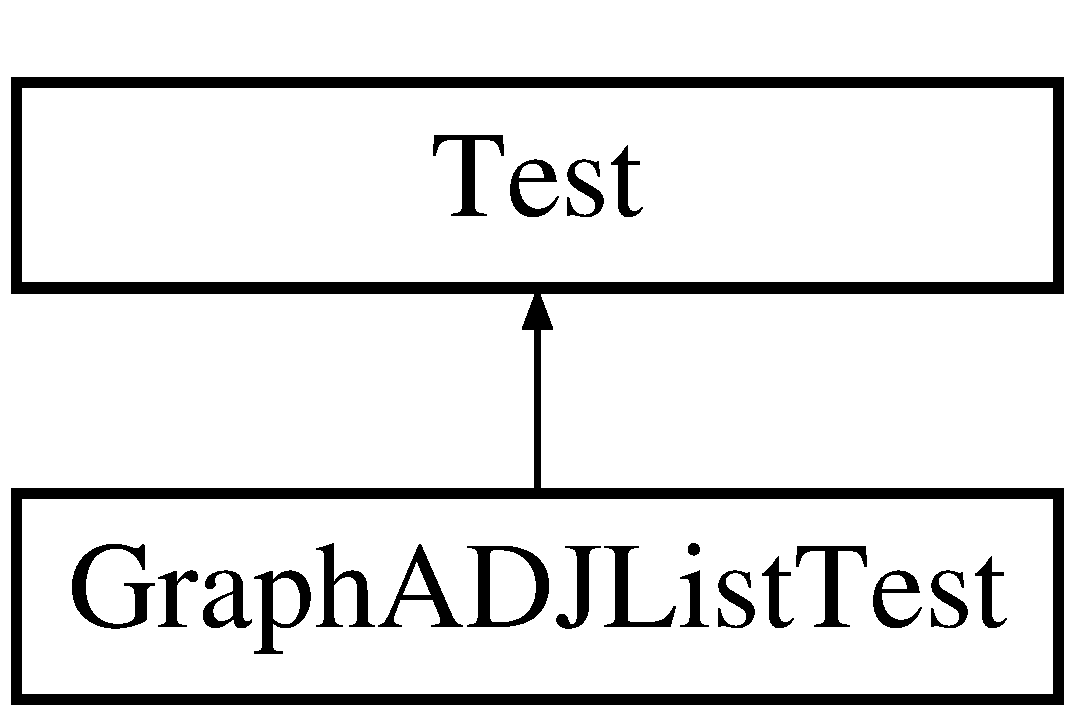
\includegraphics[height=2.000000cm]{class_graph_a_d_j_list_test}
\end{center}
\end{figure}
\subsection*{Protected Member Functions}
\begin{DoxyCompactItemize}
\item 
void \hyperlink{class_graph_a_d_j_list_test_a72021ff735af11b1db48290ea0fa8a6b}{Set\+Up} ()
\item 
void \hyperlink{class_graph_a_d_j_list_test_a79dc8e149913c35045b362c44a5fed46}{Tear\+Down} ()
\end{DoxyCompactItemize}
\subsection*{Protected Attributes}
\begin{DoxyCompactItemize}
\item 
std\+::shared\+\_\+ptr$<$ \hyperlink{struct_introduction_to_algorithm_1_1_graph_algorithm_1_1_a_d_j_list_graph}{A\+D\+J\+List\+Graph}$<$ A\+D\+J\+\_\+\+N\+U\+M $>$ $>$ \hyperlink{class_graph_a_d_j_list_test_afcd2f035a4957685bc697f296bb2b4b5}{graph}
\end{DoxyCompactItemize}


\subsection{Detailed Description}
\hyperlink{class_graph_a_d_j_list_test}{Graph\+A\+D\+J\+List\+Test}\+:测试类,用于为测试提供基础数据 

{\ttfamily \hyperlink{class_graph_a_d_j_list_test}{Graph\+A\+D\+J\+List\+Test}}是 {\ttfamily \+::testing\+::\+Test} 的子类。它主要用于为每一个{\ttfamily T\+E\+S\+T\+\_\+\+F}准备测试环境 

Definition at line 34 of file adjlistgraph\+\_\+test.\+h.



\subsection{Member Function Documentation}
\hypertarget{class_graph_a_d_j_list_test_a72021ff735af11b1db48290ea0fa8a6b}{}\index{Graph\+A\+D\+J\+List\+Test@{Graph\+A\+D\+J\+List\+Test}!Set\+Up@{Set\+Up}}
\index{Set\+Up@{Set\+Up}!Graph\+A\+D\+J\+List\+Test@{Graph\+A\+D\+J\+List\+Test}}
\subsubsection[{Set\+Up()}]{\setlength{\rightskip}{0pt plus 5cm}void Graph\+A\+D\+J\+List\+Test\+::\+Set\+Up (
\begin{DoxyParamCaption}
{}
\end{DoxyParamCaption}
)\hspace{0.3cm}{\ttfamily [inline]}, {\ttfamily [protected]}}\label{class_graph_a_d_j_list_test_a72021ff735af11b1db48290ea0fa8a6b}


Definition at line 39 of file adjlistgraph\+\_\+test.\+h.

\hypertarget{class_graph_a_d_j_list_test_a79dc8e149913c35045b362c44a5fed46}{}\index{Graph\+A\+D\+J\+List\+Test@{Graph\+A\+D\+J\+List\+Test}!Tear\+Down@{Tear\+Down}}
\index{Tear\+Down@{Tear\+Down}!Graph\+A\+D\+J\+List\+Test@{Graph\+A\+D\+J\+List\+Test}}
\subsubsection[{Tear\+Down()}]{\setlength{\rightskip}{0pt plus 5cm}void Graph\+A\+D\+J\+List\+Test\+::\+Tear\+Down (
\begin{DoxyParamCaption}
{}
\end{DoxyParamCaption}
)\hspace{0.3cm}{\ttfamily [inline]}, {\ttfamily [protected]}}\label{class_graph_a_d_j_list_test_a79dc8e149913c35045b362c44a5fed46}


Definition at line 42 of file adjlistgraph\+\_\+test.\+h.



\subsection{Member Data Documentation}
\hypertarget{class_graph_a_d_j_list_test_afcd2f035a4957685bc697f296bb2b4b5}{}\index{Graph\+A\+D\+J\+List\+Test@{Graph\+A\+D\+J\+List\+Test}!graph@{graph}}
\index{graph@{graph}!Graph\+A\+D\+J\+List\+Test@{Graph\+A\+D\+J\+List\+Test}}
\subsubsection[{graph}]{\setlength{\rightskip}{0pt plus 5cm}std\+::shared\+\_\+ptr$<${\bf A\+D\+J\+List\+Graph}$<$A\+D\+J\+\_\+\+N\+U\+M$>$ $>$ Graph\+A\+D\+J\+List\+Test\+::graph\hspace{0.3cm}{\ttfamily [protected]}}\label{class_graph_a_d_j_list_test_afcd2f035a4957685bc697f296bb2b4b5}
指向一个图 

Definition at line 44 of file adjlistgraph\+\_\+test.\+h.



The documentation for this class was generated from the following file\+:\begin{DoxyCompactItemize}
\item 
src/graph\+\_\+algorithms/basic\+\_\+graph/graph\+\_\+representation/adjlist\+\_\+graph/\hyperlink{adjlistgraph__test_8h}{adjlistgraph\+\_\+test.\+h}\end{DoxyCompactItemize}

\hypertarget{class_graph_matrix_test}{}\section{Graph\+Matrix\+Test Class Reference}
\label{class_graph_matrix_test}\index{Graph\+Matrix\+Test@{Graph\+Matrix\+Test}}


\hyperlink{class_graph_matrix_test}{Graph\+Matrix\+Test}\+:测试类,用于为测试提供基础数据  




{\ttfamily \#include $<$matrixgraph\+\_\+test.\+h$>$}

Inheritance diagram for Graph\+Matrix\+Test\+:\begin{figure}[H]
\begin{center}
\leavevmode
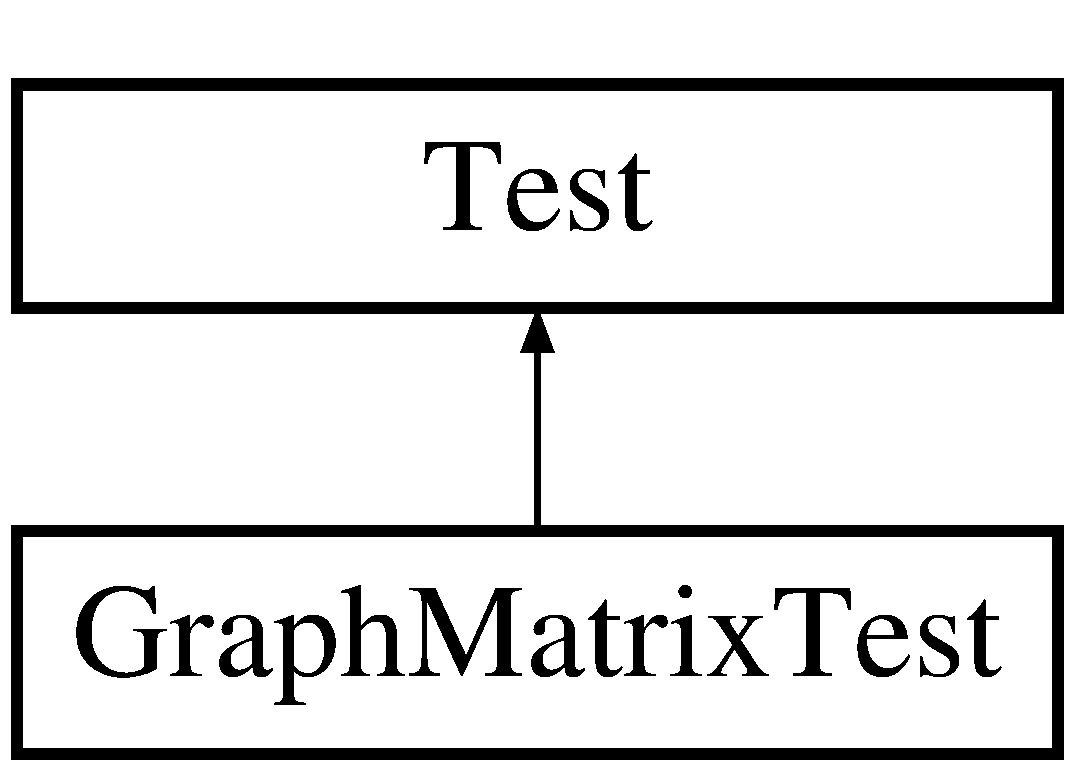
\includegraphics[height=2.000000cm]{class_graph_matrix_test}
\end{center}
\end{figure}
\subsection*{Protected Member Functions}
\begin{DoxyCompactItemize}
\item 
void \hyperlink{class_graph_matrix_test_a0bf059febd79340f3fd0a07998b86084}{Set\+Up} ()
\item 
void \hyperlink{class_graph_matrix_test_a6ecc6a16df121b02fd29a278f38083c9}{Tear\+Down} ()
\end{DoxyCompactItemize}
\subsection*{Protected Attributes}
\begin{DoxyCompactItemize}
\item 
std\+::shared\+\_\+ptr$<$ \hyperlink{struct_introduction_to_algorithm_1_1_graph_algorithm_1_1_matrix_graph}{Matrix\+Graph}$<$ M\+T\+X\+N\+U\+M $>$ $>$ \hyperlink{class_graph_matrix_test_a466258802e52f0a5408f78e809cd6d7c}{graph}
\end{DoxyCompactItemize}


\subsection{Detailed Description}
\hyperlink{class_graph_matrix_test}{Graph\+Matrix\+Test}\+:测试类,用于为测试提供基础数据 

{\ttfamily \hyperlink{class_graph_matrix_test}{Graph\+Matrix\+Test}}是 {\ttfamily \+::testing\+::\+Test} 的子类。它主要用于为每一个{\ttfamily T\+E\+S\+T\+\_\+\+F}准备测试环境 

Definition at line 34 of file matrixgraph\+\_\+test.\+h.



\subsection{Member Function Documentation}
\hypertarget{class_graph_matrix_test_a0bf059febd79340f3fd0a07998b86084}{}\index{Graph\+Matrix\+Test@{Graph\+Matrix\+Test}!Set\+Up@{Set\+Up}}
\index{Set\+Up@{Set\+Up}!Graph\+Matrix\+Test@{Graph\+Matrix\+Test}}
\subsubsection[{Set\+Up()}]{\setlength{\rightskip}{0pt plus 5cm}void Graph\+Matrix\+Test\+::\+Set\+Up (
\begin{DoxyParamCaption}
{}
\end{DoxyParamCaption}
)\hspace{0.3cm}{\ttfamily [inline]}, {\ttfamily [protected]}}\label{class_graph_matrix_test_a0bf059febd79340f3fd0a07998b86084}


Definition at line 37 of file matrixgraph\+\_\+test.\+h.

\hypertarget{class_graph_matrix_test_a6ecc6a16df121b02fd29a278f38083c9}{}\index{Graph\+Matrix\+Test@{Graph\+Matrix\+Test}!Tear\+Down@{Tear\+Down}}
\index{Tear\+Down@{Tear\+Down}!Graph\+Matrix\+Test@{Graph\+Matrix\+Test}}
\subsubsection[{Tear\+Down()}]{\setlength{\rightskip}{0pt plus 5cm}void Graph\+Matrix\+Test\+::\+Tear\+Down (
\begin{DoxyParamCaption}
{}
\end{DoxyParamCaption}
)\hspace{0.3cm}{\ttfamily [inline]}, {\ttfamily [protected]}}\label{class_graph_matrix_test_a6ecc6a16df121b02fd29a278f38083c9}


Definition at line 40 of file matrixgraph\+\_\+test.\+h.



\subsection{Member Data Documentation}
\hypertarget{class_graph_matrix_test_a466258802e52f0a5408f78e809cd6d7c}{}\index{Graph\+Matrix\+Test@{Graph\+Matrix\+Test}!graph@{graph}}
\index{graph@{graph}!Graph\+Matrix\+Test@{Graph\+Matrix\+Test}}
\subsubsection[{graph}]{\setlength{\rightskip}{0pt plus 5cm}std\+::shared\+\_\+ptr$<${\bf Matrix\+Graph}$<$M\+T\+X\+N\+U\+M$>$ $>$ Graph\+Matrix\+Test\+::graph\hspace{0.3cm}{\ttfamily [protected]}}\label{class_graph_matrix_test_a466258802e52f0a5408f78e809cd6d7c}
指向一个图 

Definition at line 42 of file matrixgraph\+\_\+test.\+h.



The documentation for this class was generated from the following file\+:\begin{DoxyCompactItemize}
\item 
src/graph\+\_\+algorithms/basic\+\_\+graph/graph\+\_\+representation/matrix\+\_\+graph/\hyperlink{matrixgraph__test_8h}{matrixgraph\+\_\+test.\+h}\end{DoxyCompactItemize}

\hypertarget{class_graph_test}{}\section{Graph\+Test Class Reference}
\label{class_graph_test}\index{Graph\+Test@{Graph\+Test}}


\hyperlink{class_graph_test}{Graph\+Test}\+:测试类,用于为测试提供基础数据  




{\ttfamily \#include $<$graph\+\_\+test.\+h$>$}

Inheritance diagram for Graph\+Test\+:\begin{figure}[H]
\begin{center}
\leavevmode
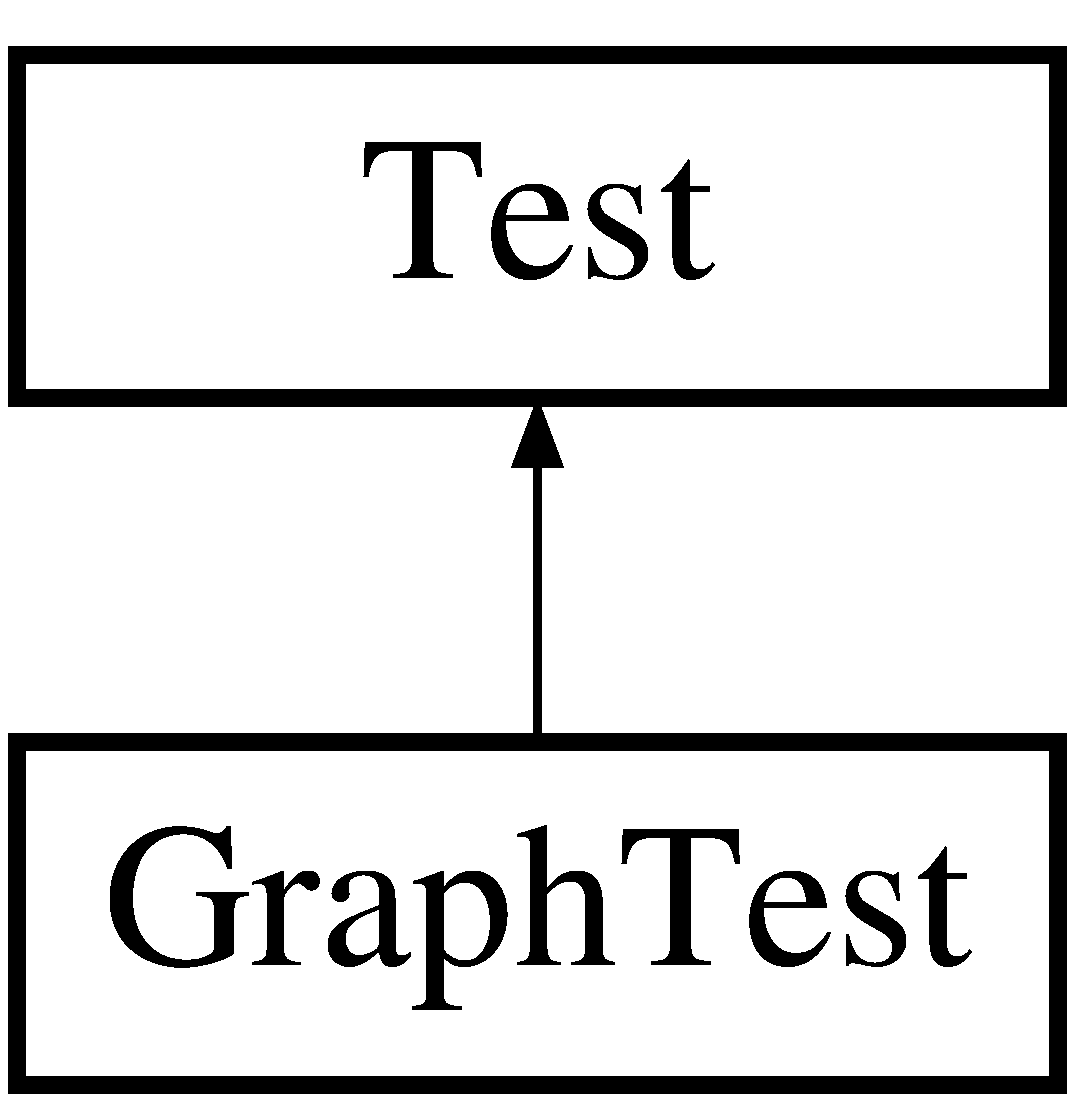
\includegraphics[height=2.000000cm]{class_graph_test}
\end{center}
\end{figure}
\subsection*{Public Types}
\begin{DoxyCompactItemize}
\item 
typedef \hyperlink{struct_introduction_to_algorithm_1_1_graph_algorithm_1_1_graph}{Graph}$<$ G\+\_\+\+N, \hyperlink{struct_introduction_to_algorithm_1_1_graph_algorithm_1_1_vertex}{Vertex}$<$ double $>$ $>$ \hyperlink{class_graph_test_a35200ea3d08690769c40550cba2ecd5a}{G\+Type}
\end{DoxyCompactItemize}
\subsection*{Protected Member Functions}
\begin{DoxyCompactItemize}
\item 
void \hyperlink{class_graph_test_a2f0d213d11ea0b8245c526379674b91b}{Set\+Up} ()
\item 
void \hyperlink{class_graph_test_a53c606b64363a694f425a844dfabc08e}{Tear\+Down} ()
\end{DoxyCompactItemize}
\subsection*{Protected Attributes}
\begin{DoxyCompactItemize}
\item 
std\+::shared\+\_\+ptr$<$ \hyperlink{class_graph_test_a35200ea3d08690769c40550cba2ecd5a}{G\+Type} $>$ \hyperlink{class_graph_test_a1dbaf4ba93fa17246e6fef78b5dd678c}{\+\_\+empty\+\_\+graph}
\item 
std\+::shared\+\_\+ptr$<$ \hyperlink{class_graph_test_a35200ea3d08690769c40550cba2ecd5a}{G\+Type} $>$ \hyperlink{class_graph_test_a2dac828599509e577b5406d06f613a16}{\+\_\+n\+\_\+vertexes\+\_\+graph}
\item 
std\+::shared\+\_\+ptr$<$ \hyperlink{class_graph_test_a35200ea3d08690769c40550cba2ecd5a}{G\+Type} $>$ \hyperlink{class_graph_test_aaa662e57a6eb46a91c59464871b4907f}{\+\_\+n\+\_\+vertexes\+\_\+m\+\_\+edges\+\_\+graph}
\end{DoxyCompactItemize}


\subsection{Detailed Description}
\hyperlink{class_graph_test}{Graph\+Test}\+:测试类,用于为测试提供基础数据 

{\ttfamily \hyperlink{class_graph_test}{Graph\+Test}}是 {\ttfamily \+::testing\+::\+Test} 的子类。它主要用于为每一个{\ttfamily T\+E\+S\+T\+\_\+\+F}准备测试环境 

Definition at line 36 of file graph\+\_\+test.\+h.



\subsection{Member Typedef Documentation}
\hypertarget{class_graph_test_a35200ea3d08690769c40550cba2ecd5a}{}\index{Graph\+Test@{Graph\+Test}!G\+Type@{G\+Type}}
\index{G\+Type@{G\+Type}!Graph\+Test@{Graph\+Test}}
\subsubsection[{G\+Type}]{\setlength{\rightskip}{0pt plus 5cm}typedef {\bf Graph}$<$G\+\_\+\+N,{\bf Vertex}$<$double$>$ $>$ {\bf Graph\+Test\+::\+G\+Type}}\label{class_graph_test_a35200ea3d08690769c40550cba2ecd5a}
模板实例化的图类型,该图的顶点类型为{\ttfamily Vertex$<$double$>$} 

Definition at line 39 of file graph\+\_\+test.\+h.



\subsection{Member Function Documentation}
\hypertarget{class_graph_test_a2f0d213d11ea0b8245c526379674b91b}{}\index{Graph\+Test@{Graph\+Test}!Set\+Up@{Set\+Up}}
\index{Set\+Up@{Set\+Up}!Graph\+Test@{Graph\+Test}}
\subsubsection[{Set\+Up()}]{\setlength{\rightskip}{0pt plus 5cm}void Graph\+Test\+::\+Set\+Up (
\begin{DoxyParamCaption}
{}
\end{DoxyParamCaption}
)\hspace{0.3cm}{\ttfamily [inline]}, {\ttfamily [protected]}}\label{class_graph_test_a2f0d213d11ea0b8245c526379674b91b}


Definition at line 42 of file graph\+\_\+test.\+h.

\hypertarget{class_graph_test_a53c606b64363a694f425a844dfabc08e}{}\index{Graph\+Test@{Graph\+Test}!Tear\+Down@{Tear\+Down}}
\index{Tear\+Down@{Tear\+Down}!Graph\+Test@{Graph\+Test}}
\subsubsection[{Tear\+Down()}]{\setlength{\rightskip}{0pt plus 5cm}void Graph\+Test\+::\+Tear\+Down (
\begin{DoxyParamCaption}
{}
\end{DoxyParamCaption}
)\hspace{0.3cm}{\ttfamily [inline]}, {\ttfamily [protected]}}\label{class_graph_test_a53c606b64363a694f425a844dfabc08e}


Definition at line 58 of file graph\+\_\+test.\+h.



\subsection{Member Data Documentation}
\hypertarget{class_graph_test_a1dbaf4ba93fa17246e6fef78b5dd678c}{}\index{Graph\+Test@{Graph\+Test}!\+\_\+empty\+\_\+graph@{\+\_\+empty\+\_\+graph}}
\index{\+\_\+empty\+\_\+graph@{\+\_\+empty\+\_\+graph}!Graph\+Test@{Graph\+Test}}
\subsubsection[{\+\_\+empty\+\_\+graph}]{\setlength{\rightskip}{0pt plus 5cm}std\+::shared\+\_\+ptr$<${\bf G\+Type}$>$ Graph\+Test\+::\+\_\+empty\+\_\+graph\hspace{0.3cm}{\ttfamily [protected]}}\label{class_graph_test_a1dbaf4ba93fa17246e6fef78b5dd678c}
指向一个空图 

Definition at line 60 of file graph\+\_\+test.\+h.

\hypertarget{class_graph_test_a2dac828599509e577b5406d06f613a16}{}\index{Graph\+Test@{Graph\+Test}!\+\_\+n\+\_\+vertexes\+\_\+graph@{\+\_\+n\+\_\+vertexes\+\_\+graph}}
\index{\+\_\+n\+\_\+vertexes\+\_\+graph@{\+\_\+n\+\_\+vertexes\+\_\+graph}!Graph\+Test@{Graph\+Test}}
\subsubsection[{\+\_\+n\+\_\+vertexes\+\_\+graph}]{\setlength{\rightskip}{0pt plus 5cm}std\+::shared\+\_\+ptr$<${\bf G\+Type}$>$ Graph\+Test\+::\+\_\+n\+\_\+vertexes\+\_\+graph\hspace{0.3cm}{\ttfamily [protected]}}\label{class_graph_test_a2dac828599509e577b5406d06f613a16}
指向一个含有n结点,0条边的图 

Definition at line 61 of file graph\+\_\+test.\+h.

\hypertarget{class_graph_test_aaa662e57a6eb46a91c59464871b4907f}{}\index{Graph\+Test@{Graph\+Test}!\+\_\+n\+\_\+vertexes\+\_\+m\+\_\+edges\+\_\+graph@{\+\_\+n\+\_\+vertexes\+\_\+m\+\_\+edges\+\_\+graph}}
\index{\+\_\+n\+\_\+vertexes\+\_\+m\+\_\+edges\+\_\+graph@{\+\_\+n\+\_\+vertexes\+\_\+m\+\_\+edges\+\_\+graph}!Graph\+Test@{Graph\+Test}}
\subsubsection[{\+\_\+n\+\_\+vertexes\+\_\+m\+\_\+edges\+\_\+graph}]{\setlength{\rightskip}{0pt plus 5cm}std\+::shared\+\_\+ptr$<${\bf G\+Type}$>$ Graph\+Test\+::\+\_\+n\+\_\+vertexes\+\_\+m\+\_\+edges\+\_\+graph\hspace{0.3cm}{\ttfamily [protected]}}\label{class_graph_test_aaa662e57a6eb46a91c59464871b4907f}
指向一个含有n结点,m条边的图 

Definition at line 62 of file graph\+\_\+test.\+h.



The documentation for this class was generated from the following file\+:\begin{DoxyCompactItemize}
\item 
src/graph\+\_\+algorithms/basic\+\_\+graph/graph\+\_\+representation/graph/\hyperlink{graph__test_8h}{graph\+\_\+test.\+h}\end{DoxyCompactItemize}

\hypertarget{class_johnson_test}{}\section{Johnson\+Test Class Reference}
\label{class_johnson_test}\index{Johnson\+Test@{Johnson\+Test}}


\hyperlink{class_johnson_test}{Johnson\+Test}\+:测试类,用于为测试提供基础数据  




{\ttfamily \#include $<$johnson\+\_\+test.\+h$>$}

Inheritance diagram for Johnson\+Test\+:\begin{figure}[H]
\begin{center}
\leavevmode
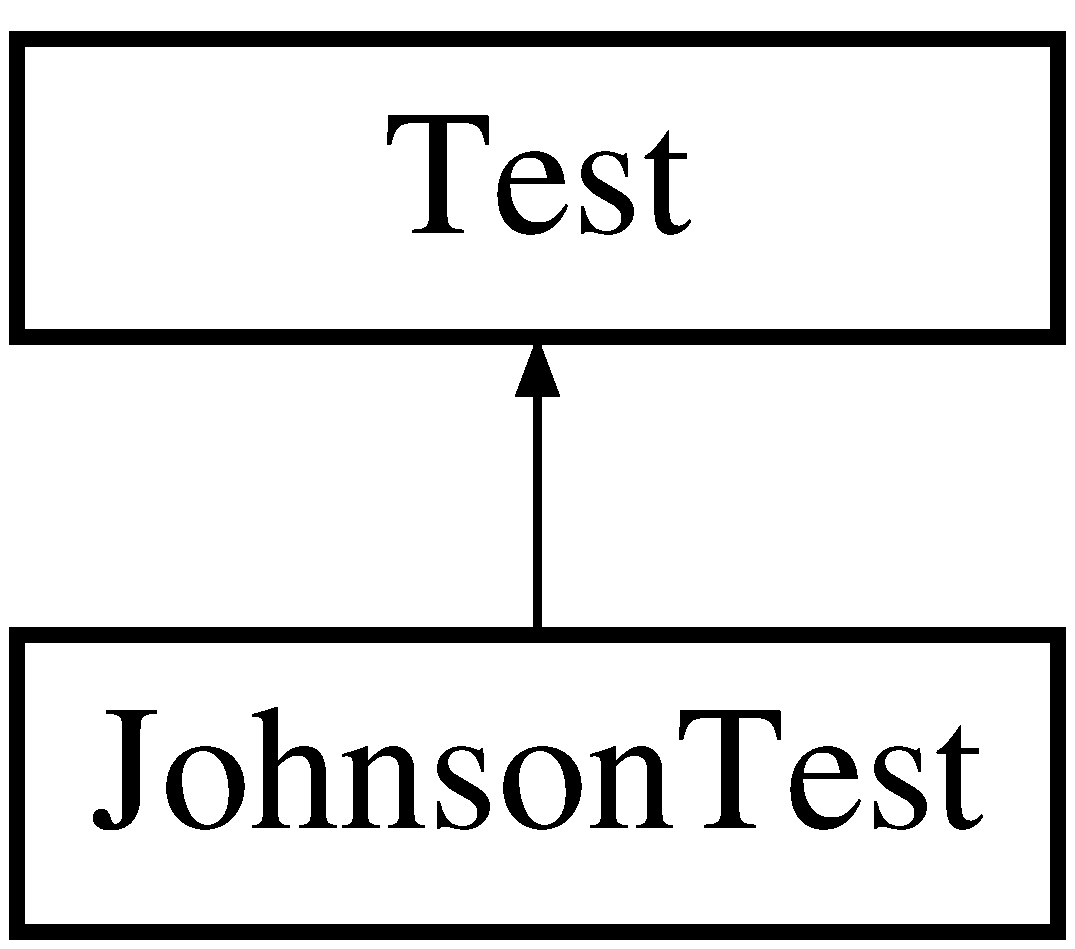
\includegraphics[height=2.000000cm]{class_johnson_test}
\end{center}
\end{figure}
\subsection*{Public Types}
\begin{DoxyCompactItemize}
\item 
typedef \hyperlink{struct_introduction_to_algorithm_1_1_graph_algorithm_1_1_graph}{Graph}$<$ J\+S\+\_\+\+N, \hyperlink{struct_introduction_to_algorithm_1_1_graph_algorithm_1_1_vertex_p}{Vertex\+P}$<$ int $>$ $>$ \hyperlink{class_johnson_test_ac738b463d046ce889761224801f56372}{G\+Type}
\end{DoxyCompactItemize}
\subsection*{Protected Member Functions}
\begin{DoxyCompactItemize}
\item 
void \hyperlink{class_johnson_test_a5bcc9c920ffcb948a3c3262e33824743}{Set\+Up} ()
\item 
void \hyperlink{class_johnson_test_a19afeaec81c858f848cabc90c64e52b8}{Tear\+Down} ()
\end{DoxyCompactItemize}
\subsection*{Protected Attributes}
\begin{DoxyCompactItemize}
\item 
std\+::shared\+\_\+ptr$<$ \hyperlink{class_johnson_test_ac738b463d046ce889761224801f56372}{G\+Type} $>$ \hyperlink{class_johnson_test_ae571863596ab15d90ed03c7f192030a3}{\+\_\+graph}
\end{DoxyCompactItemize}


\subsection{Detailed Description}
\hyperlink{class_johnson_test}{Johnson\+Test}\+:测试类,用于为测试提供基础数据 

{\ttfamily \hyperlink{class_johnson_test}{Johnson\+Test}}是 {\ttfamily \+::testing\+::\+Test} 的子类。它主要用于为每一个{\ttfamily T\+E\+S\+T\+\_\+\+F}准备测试环境 

Definition at line 40 of file johnson\+\_\+test.\+h.



\subsection{Member Typedef Documentation}
\hypertarget{class_johnson_test_ac738b463d046ce889761224801f56372}{}\index{Johnson\+Test@{Johnson\+Test}!G\+Type@{G\+Type}}
\index{G\+Type@{G\+Type}!Johnson\+Test@{Johnson\+Test}}
\subsubsection[{G\+Type}]{\setlength{\rightskip}{0pt plus 5cm}typedef {\bf Graph}$<$J\+S\+\_\+\+N,{\bf Vertex\+P}$<$int$>$ $>$ {\bf Johnson\+Test\+::\+G\+Type}}\label{class_johnson_test_ac738b463d046ce889761224801f56372}
模板实例化的图类型,该图的顶点类型为{\ttfamily Vertex\+P$<$int$>$} 

Definition at line 43 of file johnson\+\_\+test.\+h.



\subsection{Member Function Documentation}
\hypertarget{class_johnson_test_a5bcc9c920ffcb948a3c3262e33824743}{}\index{Johnson\+Test@{Johnson\+Test}!Set\+Up@{Set\+Up}}
\index{Set\+Up@{Set\+Up}!Johnson\+Test@{Johnson\+Test}}
\subsubsection[{Set\+Up()}]{\setlength{\rightskip}{0pt plus 5cm}void Johnson\+Test\+::\+Set\+Up (
\begin{DoxyParamCaption}
{}
\end{DoxyParamCaption}
)\hspace{0.3cm}{\ttfamily [inline]}, {\ttfamily [protected]}}\label{class_johnson_test_a5bcc9c920ffcb948a3c3262e33824743}


Definition at line 46 of file johnson\+\_\+test.\+h.

\hypertarget{class_johnson_test_a19afeaec81c858f848cabc90c64e52b8}{}\index{Johnson\+Test@{Johnson\+Test}!Tear\+Down@{Tear\+Down}}
\index{Tear\+Down@{Tear\+Down}!Johnson\+Test@{Johnson\+Test}}
\subsubsection[{Tear\+Down()}]{\setlength{\rightskip}{0pt plus 5cm}void Johnson\+Test\+::\+Tear\+Down (
\begin{DoxyParamCaption}
{}
\end{DoxyParamCaption}
)\hspace{0.3cm}{\ttfamily [inline]}, {\ttfamily [protected]}}\label{class_johnson_test_a19afeaec81c858f848cabc90c64e52b8}


Definition at line 64 of file johnson\+\_\+test.\+h.



\subsection{Member Data Documentation}
\hypertarget{class_johnson_test_ae571863596ab15d90ed03c7f192030a3}{}\index{Johnson\+Test@{Johnson\+Test}!\+\_\+graph@{\+\_\+graph}}
\index{\+\_\+graph@{\+\_\+graph}!Johnson\+Test@{Johnson\+Test}}
\subsubsection[{\+\_\+graph}]{\setlength{\rightskip}{0pt plus 5cm}std\+::shared\+\_\+ptr$<${\bf G\+Type}$>$ Johnson\+Test\+::\+\_\+graph\hspace{0.3cm}{\ttfamily [protected]}}\label{class_johnson_test_ae571863596ab15d90ed03c7f192030a3}
指向一个图,算法导论图25-\/1 

Definition at line 65 of file johnson\+\_\+test.\+h.



The documentation for this class was generated from the following file\+:\begin{DoxyCompactItemize}
\item 
src/graph\+\_\+algorithms/all\+\_\+node\+\_\+pair\+\_\+shortest\+\_\+path/johnson/\hyperlink{johnson__test_8h}{johnson\+\_\+test.\+h}\end{DoxyCompactItemize}

\hypertarget{class_kruskal_test}{}\section{Kruskal\+Test Class Reference}
\label{class_kruskal_test}\index{Kruskal\+Test@{Kruskal\+Test}}


\hyperlink{class_kruskal_test}{Kruskal\+Test}\+:测试类,用于为测试提供基础数据  




{\ttfamily \#include $<$kruskal\+\_\+test.\+h$>$}

Inheritance diagram for Kruskal\+Test\+:\begin{figure}[H]
\begin{center}
\leavevmode
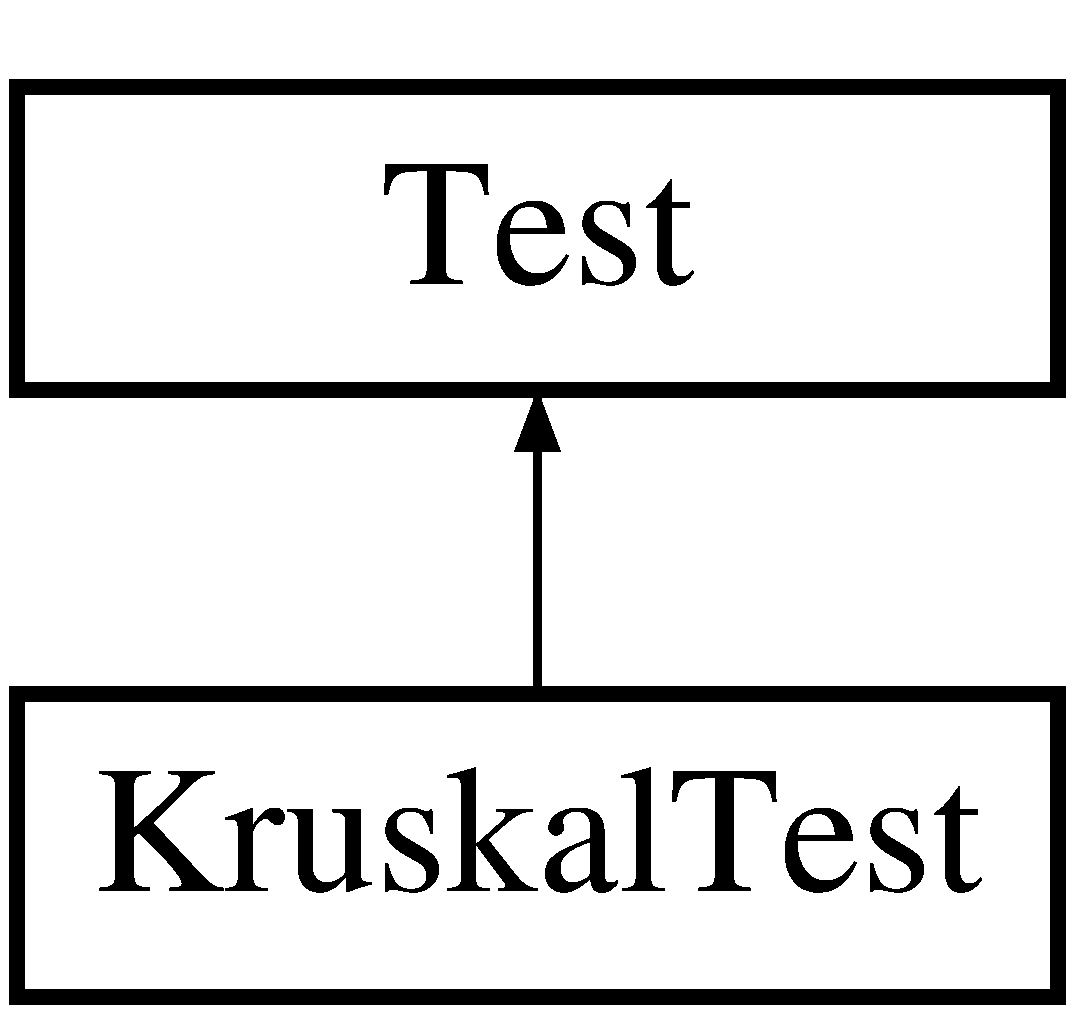
\includegraphics[height=2.000000cm]{class_kruskal_test}
\end{center}
\end{figure}
\subsection*{Public Types}
\begin{DoxyCompactItemize}
\item 
typedef \hyperlink{struct_introduction_to_algorithm_1_1_graph_algorithm_1_1_graph}{Graph}$<$ K\+\_\+\+N\+U\+M, \hyperlink{struct_introduction_to_algorithm_1_1_graph_algorithm_1_1_set_vertex}{Set\+Vertex}$<$ int $>$ $>$ \hyperlink{class_kruskal_test_a4cf4187bb360392a6e5829dacdf6fd6c}{G\+Type}
\item 
typedef std\+::function$<$ void(\hyperlink{struct_introduction_to_algorithm_1_1_graph_algorithm_1_1_set_vertex}{Set\+Vertex}$<$ int $>$\+::V\+I\+D\+Type,\hyperlink{struct_introduction_to_algorithm_1_1_graph_algorithm_1_1_set_vertex}{Set\+Vertex}$<$ int $>$\+::V\+I\+D\+Type)$>$ \hyperlink{class_kruskal_test_aa93c0a0f0cb0efdaeb56ea76b6861bef}{Action\+Type}
\end{DoxyCompactItemize}
\subsection*{Protected Member Functions}
\begin{DoxyCompactItemize}
\item 
void \hyperlink{class_kruskal_test_a8dec8e2cc34987a27862ce70a4557a39}{Set\+Up} ()
\item 
void \hyperlink{class_kruskal_test_afd7bb087cf8a63329181fc7a34b81625}{Tear\+Down} ()
\end{DoxyCompactItemize}
\subsection*{Protected Attributes}
\begin{DoxyCompactItemize}
\item 
std\+::shared\+\_\+ptr$<$ \hyperlink{class_kruskal_test_a4cf4187bb360392a6e5829dacdf6fd6c}{G\+Type} $>$ \hyperlink{class_kruskal_test_a10424b1b5e9d63288d1751ee0e6115b4}{\+\_\+1v\+\_\+graph}
\item 
std\+::shared\+\_\+ptr$<$ \hyperlink{class_kruskal_test_a4cf4187bb360392a6e5829dacdf6fd6c}{G\+Type} $>$ \hyperlink{class_kruskal_test_ac4ef5fe84afa9d1774edd0f0d8e31e48}{\+\_\+1e\+\_\+graph}
\item 
std\+::shared\+\_\+ptr$<$ \hyperlink{class_kruskal_test_a4cf4187bb360392a6e5829dacdf6fd6c}{G\+Type} $>$ \hyperlink{class_kruskal_test_ac63161fae446d5ec15c82562d81b0d45}{\+\_\+list\+\_\+graph}
\item 
std\+::shared\+\_\+ptr$<$ \hyperlink{class_kruskal_test_a4cf4187bb360392a6e5829dacdf6fd6c}{G\+Type} $>$ \hyperlink{class_kruskal_test_a70183c9dedc39d09d71da4b3cecb59a4}{\+\_\+all\+\_\+edges\+\_\+graph}
\end{DoxyCompactItemize}


\subsection{Detailed Description}
\hyperlink{class_kruskal_test}{Kruskal\+Test}\+:测试类,用于为测试提供基础数据 

{\ttfamily \hyperlink{class_kruskal_test}{Kruskal\+Test}}是 {\ttfamily \+::testing\+::\+Test} 的子类。它主要用于为每一个{\ttfamily T\+E\+S\+T\+\_\+\+F}准备测试环境 

Definition at line 38 of file kruskal\+\_\+test.\+h.



\subsection{Member Typedef Documentation}
\hypertarget{class_kruskal_test_aa93c0a0f0cb0efdaeb56ea76b6861bef}{}\index{Kruskal\+Test@{Kruskal\+Test}!Action\+Type@{Action\+Type}}
\index{Action\+Type@{Action\+Type}!Kruskal\+Test@{Kruskal\+Test}}
\subsubsection[{Action\+Type}]{\setlength{\rightskip}{0pt plus 5cm}typedef std\+::function$<$void({\bf Set\+Vertex}$<$int$>$\+::V\+I\+D\+Type ,{\bf Set\+Vertex}$<$int$>$\+::V\+I\+D\+Type)$>$ {\bf Kruskal\+Test\+::\+Action\+Type}}\label{class_kruskal_test_aa93c0a0f0cb0efdaeb56ea76b6861bef}
模板实例化的\+Action类型 

Definition at line 42 of file kruskal\+\_\+test.\+h.

\hypertarget{class_kruskal_test_a4cf4187bb360392a6e5829dacdf6fd6c}{}\index{Kruskal\+Test@{Kruskal\+Test}!G\+Type@{G\+Type}}
\index{G\+Type@{G\+Type}!Kruskal\+Test@{Kruskal\+Test}}
\subsubsection[{G\+Type}]{\setlength{\rightskip}{0pt plus 5cm}typedef {\bf Graph}$<$K\+\_\+\+N\+U\+M,{\bf Set\+Vertex}$<$int$>$ $>$ {\bf Kruskal\+Test\+::\+G\+Type}}\label{class_kruskal_test_a4cf4187bb360392a6e5829dacdf6fd6c}
模板实例化的图类型,该图的顶点类型为{\ttfamily Set\+Vertex$<$int$>$} 

Definition at line 41 of file kruskal\+\_\+test.\+h.



\subsection{Member Function Documentation}
\hypertarget{class_kruskal_test_a8dec8e2cc34987a27862ce70a4557a39}{}\index{Kruskal\+Test@{Kruskal\+Test}!Set\+Up@{Set\+Up}}
\index{Set\+Up@{Set\+Up}!Kruskal\+Test@{Kruskal\+Test}}
\subsubsection[{Set\+Up()}]{\setlength{\rightskip}{0pt plus 5cm}void Kruskal\+Test\+::\+Set\+Up (
\begin{DoxyParamCaption}
{}
\end{DoxyParamCaption}
)\hspace{0.3cm}{\ttfamily [inline]}, {\ttfamily [protected]}}\label{class_kruskal_test_a8dec8e2cc34987a27862ce70a4557a39}


Definition at line 44 of file kruskal\+\_\+test.\+h.

\hypertarget{class_kruskal_test_afd7bb087cf8a63329181fc7a34b81625}{}\index{Kruskal\+Test@{Kruskal\+Test}!Tear\+Down@{Tear\+Down}}
\index{Tear\+Down@{Tear\+Down}!Kruskal\+Test@{Kruskal\+Test}}
\subsubsection[{Tear\+Down()}]{\setlength{\rightskip}{0pt plus 5cm}void Kruskal\+Test\+::\+Tear\+Down (
\begin{DoxyParamCaption}
{}
\end{DoxyParamCaption}
)\hspace{0.3cm}{\ttfamily [inline]}, {\ttfamily [protected]}}\label{class_kruskal_test_afd7bb087cf8a63329181fc7a34b81625}


Definition at line 72 of file kruskal\+\_\+test.\+h.



\subsection{Member Data Documentation}
\hypertarget{class_kruskal_test_ac4ef5fe84afa9d1774edd0f0d8e31e48}{}\index{Kruskal\+Test@{Kruskal\+Test}!\+\_\+1e\+\_\+graph@{\+\_\+1e\+\_\+graph}}
\index{\+\_\+1e\+\_\+graph@{\+\_\+1e\+\_\+graph}!Kruskal\+Test@{Kruskal\+Test}}
\subsubsection[{\+\_\+1e\+\_\+graph}]{\setlength{\rightskip}{0pt plus 5cm}std\+::shared\+\_\+ptr$<${\bf G\+Type}$>$ Kruskal\+Test\+::\+\_\+1e\+\_\+graph\hspace{0.3cm}{\ttfamily [protected]}}\label{class_kruskal_test_ac4ef5fe84afa9d1774edd0f0d8e31e48}
指向一个图,该图只有一条边 

Definition at line 74 of file kruskal\+\_\+test.\+h.

\hypertarget{class_kruskal_test_a10424b1b5e9d63288d1751ee0e6115b4}{}\index{Kruskal\+Test@{Kruskal\+Test}!\+\_\+1v\+\_\+graph@{\+\_\+1v\+\_\+graph}}
\index{\+\_\+1v\+\_\+graph@{\+\_\+1v\+\_\+graph}!Kruskal\+Test@{Kruskal\+Test}}
\subsubsection[{\+\_\+1v\+\_\+graph}]{\setlength{\rightskip}{0pt plus 5cm}std\+::shared\+\_\+ptr$<${\bf G\+Type}$>$ Kruskal\+Test\+::\+\_\+1v\+\_\+graph\hspace{0.3cm}{\ttfamily [protected]}}\label{class_kruskal_test_a10424b1b5e9d63288d1751ee0e6115b4}
指向一个图,该图只有一个顶点 

Definition at line 73 of file kruskal\+\_\+test.\+h.

\hypertarget{class_kruskal_test_a70183c9dedc39d09d71da4b3cecb59a4}{}\index{Kruskal\+Test@{Kruskal\+Test}!\+\_\+all\+\_\+edges\+\_\+graph@{\+\_\+all\+\_\+edges\+\_\+graph}}
\index{\+\_\+all\+\_\+edges\+\_\+graph@{\+\_\+all\+\_\+edges\+\_\+graph}!Kruskal\+Test@{Kruskal\+Test}}
\subsubsection[{\+\_\+all\+\_\+edges\+\_\+graph}]{\setlength{\rightskip}{0pt plus 5cm}std\+::shared\+\_\+ptr$<${\bf G\+Type}$>$ Kruskal\+Test\+::\+\_\+all\+\_\+edges\+\_\+graph\hspace{0.3cm}{\ttfamily [protected]}}\label{class_kruskal_test_a70183c9dedc39d09d71da4b3cecb59a4}
指向一个图,该图中任意一对顶点之间都有边 

Definition at line 76 of file kruskal\+\_\+test.\+h.

\hypertarget{class_kruskal_test_ac63161fae446d5ec15c82562d81b0d45}{}\index{Kruskal\+Test@{Kruskal\+Test}!\+\_\+list\+\_\+graph@{\+\_\+list\+\_\+graph}}
\index{\+\_\+list\+\_\+graph@{\+\_\+list\+\_\+graph}!Kruskal\+Test@{Kruskal\+Test}}
\subsubsection[{\+\_\+list\+\_\+graph}]{\setlength{\rightskip}{0pt plus 5cm}std\+::shared\+\_\+ptr$<${\bf G\+Type}$>$ Kruskal\+Test\+::\+\_\+list\+\_\+graph\hspace{0.3cm}{\ttfamily [protected]}}\label{class_kruskal_test_ac63161fae446d5ec15c82562d81b0d45}
指向一个图,该图的边组成一个链条 

Definition at line 75 of file kruskal\+\_\+test.\+h.



The documentation for this class was generated from the following file\+:\begin{DoxyCompactItemize}
\item 
src/graph\+\_\+algorithms/minimum\+\_\+spanning\+\_\+tree/kruskal/\hyperlink{kruskal__test_8h}{kruskal\+\_\+test.\+h}\end{DoxyCompactItemize}

\hypertarget{struct_introduction_to_algorithm_1_1_graph_algorithm_1_1_list}{}\section{Introduction\+To\+Algorithm\+:\+:Graph\+Algorithm\+:\+:List$<$ Node\+Type $>$ Struct Template Reference}
\label{struct_introduction_to_algorithm_1_1_graph_algorithm_1_1_list}\index{Introduction\+To\+Algorithm\+::\+Graph\+Algorithm\+::\+List$<$ Node\+Type $>$@{Introduction\+To\+Algorithm\+::\+Graph\+Algorithm\+::\+List$<$ Node\+Type $>$}}


List:链表数据结构  




{\ttfamily \#include $<$front\+\_\+flow\+\_\+vertex.\+h$>$}

\subsection*{Public Member Functions}
\begin{DoxyCompactItemize}
\item 
\hyperlink{struct_introduction_to_algorithm_1_1_graph_algorithm_1_1_list_a286b76ddec66a739312a2f5cef3ae544}{List} ()
\begin{DoxyCompactList}\small\item\em List默认构造函数 \end{DoxyCompactList}\item 
void \hyperlink{struct_introduction_to_algorithm_1_1_graph_algorithm_1_1_list_a03267a13e44d42586d44460d04138cc1}{add} (std\+::shared\+\_\+ptr$<$ Node\+Type $>$ element)
\begin{DoxyCompactList}\small\item\em add\+:添加元素 \end{DoxyCompactList}\item 
std\+::shared\+\_\+ptr$<$ Node\+Type $>$ \hyperlink{struct_introduction_to_algorithm_1_1_graph_algorithm_1_1_list_abd886aeac60fbdfa0290cafd7d67b718}{front\+\_\+of} (std\+::shared\+\_\+ptr$<$ Node\+Type $>$ element) const 
\begin{DoxyCompactList}\small\item\em front\+\_\+of\+:链表指定元素前面的元素 \end{DoxyCompactList}\item 
std\+::string \hyperlink{struct_introduction_to_algorithm_1_1_graph_algorithm_1_1_list_a7a75e61d7a61923e5b185e1b4781d29f}{to\+\_\+string} () const 
\begin{DoxyCompactList}\small\item\em to\+\_\+string:返回链表的字符串描述 \end{DoxyCompactList}\end{DoxyCompactItemize}
\subsection*{Public Attributes}
\begin{DoxyCompactItemize}
\item 
std\+::shared\+\_\+ptr$<$ Node\+Type $>$ \hyperlink{struct_introduction_to_algorithm_1_1_graph_algorithm_1_1_list_a78a07f79c1c8133b74f23ec794e0557e}{head}
\item 
std\+::shared\+\_\+ptr$<$ Node\+Type $>$ \hyperlink{struct_introduction_to_algorithm_1_1_graph_algorithm_1_1_list_ad321a5c55f1f58c6054b7925ea007f89}{current}
\end{DoxyCompactItemize}


\subsection{Detailed Description}
\subsubsection*{template$<$typename Node\+Type$>$struct Introduction\+To\+Algorithm\+::\+Graph\+Algorithm\+::\+List$<$ Node\+Type $>$}

List:链表数据结构 

链表包含两个数据成员:


\begin{DoxyItemize}
\item head:指向链表头部的元素的强指针
\item current\+:指向链表当前处理元素的强指针 
\end{DoxyItemize}

Definition at line 37 of file front\+\_\+flow\+\_\+vertex.\+h.



\subsection{Constructor \& Destructor Documentation}
\hypertarget{struct_introduction_to_algorithm_1_1_graph_algorithm_1_1_list_a286b76ddec66a739312a2f5cef3ae544}{}\index{Introduction\+To\+Algorithm\+::\+Graph\+Algorithm\+::\+List@{Introduction\+To\+Algorithm\+::\+Graph\+Algorithm\+::\+List}!List@{List}}
\index{List@{List}!Introduction\+To\+Algorithm\+::\+Graph\+Algorithm\+::\+List@{Introduction\+To\+Algorithm\+::\+Graph\+Algorithm\+::\+List}}
\subsubsection[{List()}]{\setlength{\rightskip}{0pt plus 5cm}template$<$typename Node\+Type$>$ {\bf Introduction\+To\+Algorithm\+::\+Graph\+Algorithm\+::\+List}$<$ Node\+Type $>$\+::{\bf List} (
\begin{DoxyParamCaption}
{}
\end{DoxyParamCaption}
)\hspace{0.3cm}{\ttfamily [inline]}}\label{struct_introduction_to_algorithm_1_1_graph_algorithm_1_1_list_a286b76ddec66a739312a2f5cef3ae544}


List默认构造函数 

默认构造函数完成两个设置:head设为空指针,current设为空指针 

Definition at line 48 of file front\+\_\+flow\+\_\+vertex.\+h.



\subsection{Member Function Documentation}
\hypertarget{struct_introduction_to_algorithm_1_1_graph_algorithm_1_1_list_a03267a13e44d42586d44460d04138cc1}{}\index{Introduction\+To\+Algorithm\+::\+Graph\+Algorithm\+::\+List@{Introduction\+To\+Algorithm\+::\+Graph\+Algorithm\+::\+List}!add@{add}}
\index{add@{add}!Introduction\+To\+Algorithm\+::\+Graph\+Algorithm\+::\+List@{Introduction\+To\+Algorithm\+::\+Graph\+Algorithm\+::\+List}}
\subsubsection[{add(std\+::shared\+\_\+ptr$<$ Node\+Type $>$ element)}]{\setlength{\rightskip}{0pt plus 5cm}template$<$typename Node\+Type$>$ void {\bf Introduction\+To\+Algorithm\+::\+Graph\+Algorithm\+::\+List}$<$ Node\+Type $>$\+::add (
\begin{DoxyParamCaption}
\item[{std\+::shared\+\_\+ptr$<$ Node\+Type $>$}]{element}
\end{DoxyParamCaption}
)\hspace{0.3cm}{\ttfamily [inline]}}\label{struct_introduction_to_algorithm_1_1_graph_algorithm_1_1_list_a03267a13e44d42586d44460d04138cc1}


add\+:添加元素 


\begin{DoxyParams}{Parameters}
{\em element\+:被添加元素的强指针} & 若element为空指针则直接返回;否则将element添加到表头 \\
\hline
\end{DoxyParams}


Definition at line 58 of file front\+\_\+flow\+\_\+vertex.\+h.

\hypertarget{struct_introduction_to_algorithm_1_1_graph_algorithm_1_1_list_abd886aeac60fbdfa0290cafd7d67b718}{}\index{Introduction\+To\+Algorithm\+::\+Graph\+Algorithm\+::\+List@{Introduction\+To\+Algorithm\+::\+Graph\+Algorithm\+::\+List}!front\+\_\+of@{front\+\_\+of}}
\index{front\+\_\+of@{front\+\_\+of}!Introduction\+To\+Algorithm\+::\+Graph\+Algorithm\+::\+List@{Introduction\+To\+Algorithm\+::\+Graph\+Algorithm\+::\+List}}
\subsubsection[{front\+\_\+of(std\+::shared\+\_\+ptr$<$ Node\+Type $>$ element) const }]{\setlength{\rightskip}{0pt plus 5cm}template$<$typename Node\+Type$>$ std\+::shared\+\_\+ptr$<$Node\+Type$>$ {\bf Introduction\+To\+Algorithm\+::\+Graph\+Algorithm\+::\+List}$<$ Node\+Type $>$\+::front\+\_\+of (
\begin{DoxyParamCaption}
\item[{std\+::shared\+\_\+ptr$<$ Node\+Type $>$}]{element}
\end{DoxyParamCaption}
) const\hspace{0.3cm}{\ttfamily [inline]}}\label{struct_introduction_to_algorithm_1_1_graph_algorithm_1_1_list_abd886aeac60fbdfa0290cafd7d67b718}


front\+\_\+of\+:链表指定元素前面的元素 


\begin{DoxyParams}{Parameters}
{\em element\+:指定的元素} & \\
\hline
\end{DoxyParams}
\begin{DoxyReturn}{Returns}
\+:指定元素前面元素的强指针
\end{DoxyReturn}
若element为空指针则抛出异常。否则遍历列表。若找到指定元素,则返回其前面元素的指针;若找不到指定元素, 则抛出异常 

Definition at line 81 of file front\+\_\+flow\+\_\+vertex.\+h.

\hypertarget{struct_introduction_to_algorithm_1_1_graph_algorithm_1_1_list_a7a75e61d7a61923e5b185e1b4781d29f}{}\index{Introduction\+To\+Algorithm\+::\+Graph\+Algorithm\+::\+List@{Introduction\+To\+Algorithm\+::\+Graph\+Algorithm\+::\+List}!to\+\_\+string@{to\+\_\+string}}
\index{to\+\_\+string@{to\+\_\+string}!Introduction\+To\+Algorithm\+::\+Graph\+Algorithm\+::\+List@{Introduction\+To\+Algorithm\+::\+Graph\+Algorithm\+::\+List}}
\subsubsection[{to\+\_\+string() const }]{\setlength{\rightskip}{0pt plus 5cm}template$<$typename Node\+Type$>$ std\+::string {\bf Introduction\+To\+Algorithm\+::\+Graph\+Algorithm\+::\+List}$<$ Node\+Type $>$\+::to\+\_\+string (
\begin{DoxyParamCaption}
{}
\end{DoxyParamCaption}
) const\hspace{0.3cm}{\ttfamily [inline]}}\label{struct_introduction_to_algorithm_1_1_graph_algorithm_1_1_list_a7a75e61d7a61923e5b185e1b4781d29f}


to\+\_\+string:返回链表的字符串描述 

\begin{DoxyReturn}{Returns}
\+:链表的字符串描述
\end{DoxyReturn}
依次拼接各结点的字符串描述 

Definition at line 106 of file front\+\_\+flow\+\_\+vertex.\+h.



\subsection{Member Data Documentation}
\hypertarget{struct_introduction_to_algorithm_1_1_graph_algorithm_1_1_list_ad321a5c55f1f58c6054b7925ea007f89}{}\index{Introduction\+To\+Algorithm\+::\+Graph\+Algorithm\+::\+List@{Introduction\+To\+Algorithm\+::\+Graph\+Algorithm\+::\+List}!current@{current}}
\index{current@{current}!Introduction\+To\+Algorithm\+::\+Graph\+Algorithm\+::\+List@{Introduction\+To\+Algorithm\+::\+Graph\+Algorithm\+::\+List}}
\subsubsection[{current}]{\setlength{\rightskip}{0pt plus 5cm}template$<$typename Node\+Type$>$ std\+::shared\+\_\+ptr$<$Node\+Type$>$ {\bf Introduction\+To\+Algorithm\+::\+Graph\+Algorithm\+::\+List}$<$ Node\+Type $>$\+::current}\label{struct_introduction_to_algorithm_1_1_graph_algorithm_1_1_list_ad321a5c55f1f58c6054b7925ea007f89}
指向链表当前处理元素的强指针 

Definition at line 40 of file front\+\_\+flow\+\_\+vertex.\+h.

\hypertarget{struct_introduction_to_algorithm_1_1_graph_algorithm_1_1_list_a78a07f79c1c8133b74f23ec794e0557e}{}\index{Introduction\+To\+Algorithm\+::\+Graph\+Algorithm\+::\+List@{Introduction\+To\+Algorithm\+::\+Graph\+Algorithm\+::\+List}!head@{head}}
\index{head@{head}!Introduction\+To\+Algorithm\+::\+Graph\+Algorithm\+::\+List@{Introduction\+To\+Algorithm\+::\+Graph\+Algorithm\+::\+List}}
\subsubsection[{head}]{\setlength{\rightskip}{0pt plus 5cm}template$<$typename Node\+Type$>$ std\+::shared\+\_\+ptr$<$Node\+Type$>$ {\bf Introduction\+To\+Algorithm\+::\+Graph\+Algorithm\+::\+List}$<$ Node\+Type $>$\+::head}\label{struct_introduction_to_algorithm_1_1_graph_algorithm_1_1_list_a78a07f79c1c8133b74f23ec794e0557e}
指向链表头部的元素的强指针 

Definition at line 39 of file front\+\_\+flow\+\_\+vertex.\+h.



The documentation for this struct was generated from the following file\+:\begin{DoxyCompactItemize}
\item 
src/graph\+\_\+algorithms/basic\+\_\+graph/graph\+\_\+representation/graph\+\_\+vertex/\hyperlink{front__flow__vertex_8h}{front\+\_\+flow\+\_\+vertex.\+h}\end{DoxyCompactItemize}

\hypertarget{struct_introduction_to_algorithm_1_1_graph_algorithm_1_1_list_node}{}\section{Introduction\+To\+Algorithm\+:\+:Graph\+Algorithm\+:\+:List\+Node$<$ Value\+Type $>$ Struct Template Reference}
\label{struct_introduction_to_algorithm_1_1_graph_algorithm_1_1_list_node}\index{Introduction\+To\+Algorithm\+::\+Graph\+Algorithm\+::\+List\+Node$<$ Value\+Type $>$@{Introduction\+To\+Algorithm\+::\+Graph\+Algorithm\+::\+List\+Node$<$ Value\+Type $>$}}


List\+Node:链表结点的数据结构  




{\ttfamily \#include $<$front\+\_\+flow\+\_\+vertex.\+h$>$}

\subsection*{Public Member Functions}
\begin{DoxyCompactItemize}
\item 
\hyperlink{struct_introduction_to_algorithm_1_1_graph_algorithm_1_1_list_node_a28a10edc3e4414f2b3f41945bb886be4}{List\+Node} ()
\begin{DoxyCompactList}\small\item\em List\+Node默认构造函数 \end{DoxyCompactList}\item 
std\+::string \hyperlink{struct_introduction_to_algorithm_1_1_graph_algorithm_1_1_list_node_a09b7805e42547e2cf808e6be7b202be5}{to\+\_\+string} () const 
\begin{DoxyCompactList}\small\item\em to\+\_\+string:返回结点的字符串描述 \end{DoxyCompactList}\end{DoxyCompactItemize}
\subsection*{Public Attributes}
\begin{DoxyCompactItemize}
\item 
std\+::weak\+\_\+ptr$<$ Value\+Type $>$ \hyperlink{struct_introduction_to_algorithm_1_1_graph_algorithm_1_1_list_node_a77c644bba4a2996906d1d5b5be300b00}{value}
\item 
std\+::shared\+\_\+ptr$<$ \hyperlink{struct_introduction_to_algorithm_1_1_graph_algorithm_1_1_list_node}{List\+Node} $>$ \hyperlink{struct_introduction_to_algorithm_1_1_graph_algorithm_1_1_list_node_a78e88960b96014607258bf721c2023d1}{next}
\end{DoxyCompactItemize}


\subsection{Detailed Description}
\subsubsection*{template$<$typename Value\+Type$>$struct Introduction\+To\+Algorithm\+::\+Graph\+Algorithm\+::\+List\+Node$<$ Value\+Type $>$}

List\+Node:链表结点的数据结构 

链表结点包含两个数据成员:


\begin{DoxyItemize}
\item value:链表结点保存数据的弱指针(因为该保存数据有个强指针指向本结点)
\item next\+:指向本链表中当前结点的下一个结点的强指针 
\end{DoxyItemize}

Definition at line 133 of file front\+\_\+flow\+\_\+vertex.\+h.



\subsection{Constructor \& Destructor Documentation}
\hypertarget{struct_introduction_to_algorithm_1_1_graph_algorithm_1_1_list_node_a28a10edc3e4414f2b3f41945bb886be4}{}\index{Introduction\+To\+Algorithm\+::\+Graph\+Algorithm\+::\+List\+Node@{Introduction\+To\+Algorithm\+::\+Graph\+Algorithm\+::\+List\+Node}!List\+Node@{List\+Node}}
\index{List\+Node@{List\+Node}!Introduction\+To\+Algorithm\+::\+Graph\+Algorithm\+::\+List\+Node@{Introduction\+To\+Algorithm\+::\+Graph\+Algorithm\+::\+List\+Node}}
\subsubsection[{List\+Node()}]{\setlength{\rightskip}{0pt plus 5cm}template$<$typename Value\+Type $>$ {\bf Introduction\+To\+Algorithm\+::\+Graph\+Algorithm\+::\+List\+Node}$<$ Value\+Type $>$\+::{\bf List\+Node} (
\begin{DoxyParamCaption}
{}
\end{DoxyParamCaption}
)\hspace{0.3cm}{\ttfamily [inline]}}\label{struct_introduction_to_algorithm_1_1_graph_algorithm_1_1_list_node_a28a10edc3e4414f2b3f41945bb886be4}


List\+Node默认构造函数 

默认构造函数完成两个设置:value设为空指针,next设为空指针 

Definition at line 141 of file front\+\_\+flow\+\_\+vertex.\+h.



\subsection{Member Function Documentation}
\hypertarget{struct_introduction_to_algorithm_1_1_graph_algorithm_1_1_list_node_a09b7805e42547e2cf808e6be7b202be5}{}\index{Introduction\+To\+Algorithm\+::\+Graph\+Algorithm\+::\+List\+Node@{Introduction\+To\+Algorithm\+::\+Graph\+Algorithm\+::\+List\+Node}!to\+\_\+string@{to\+\_\+string}}
\index{to\+\_\+string@{to\+\_\+string}!Introduction\+To\+Algorithm\+::\+Graph\+Algorithm\+::\+List\+Node@{Introduction\+To\+Algorithm\+::\+Graph\+Algorithm\+::\+List\+Node}}
\subsubsection[{to\+\_\+string() const }]{\setlength{\rightskip}{0pt plus 5cm}template$<$typename Value\+Type $>$ std\+::string {\bf Introduction\+To\+Algorithm\+::\+Graph\+Algorithm\+::\+List\+Node}$<$ Value\+Type $>$\+::to\+\_\+string (
\begin{DoxyParamCaption}
{}
\end{DoxyParamCaption}
) const\hspace{0.3cm}{\ttfamily [inline]}}\label{struct_introduction_to_algorithm_1_1_graph_algorithm_1_1_list_node_a09b7805e42547e2cf808e6be7b202be5}


to\+\_\+string:返回结点的字符串描述 

\begin{DoxyReturn}{Returns}
\+:顶点的字符串描述
\end{DoxyReturn}
主要是返回 {\ttfamily value}成员的字符串描述 

Definition at line 150 of file front\+\_\+flow\+\_\+vertex.\+h.



\subsection{Member Data Documentation}
\hypertarget{struct_introduction_to_algorithm_1_1_graph_algorithm_1_1_list_node_a78e88960b96014607258bf721c2023d1}{}\index{Introduction\+To\+Algorithm\+::\+Graph\+Algorithm\+::\+List\+Node@{Introduction\+To\+Algorithm\+::\+Graph\+Algorithm\+::\+List\+Node}!next@{next}}
\index{next@{next}!Introduction\+To\+Algorithm\+::\+Graph\+Algorithm\+::\+List\+Node@{Introduction\+To\+Algorithm\+::\+Graph\+Algorithm\+::\+List\+Node}}
\subsubsection[{next}]{\setlength{\rightskip}{0pt plus 5cm}template$<$typename Value\+Type $>$ std\+::shared\+\_\+ptr$<${\bf List\+Node}$>$ {\bf Introduction\+To\+Algorithm\+::\+Graph\+Algorithm\+::\+List\+Node}$<$ Value\+Type $>$\+::next}\label{struct_introduction_to_algorithm_1_1_graph_algorithm_1_1_list_node_a78e88960b96014607258bf721c2023d1}
指向本链表中当前结点的下一个结点的强指针 

Definition at line 143 of file front\+\_\+flow\+\_\+vertex.\+h.

\hypertarget{struct_introduction_to_algorithm_1_1_graph_algorithm_1_1_list_node_a77c644bba4a2996906d1d5b5be300b00}{}\index{Introduction\+To\+Algorithm\+::\+Graph\+Algorithm\+::\+List\+Node@{Introduction\+To\+Algorithm\+::\+Graph\+Algorithm\+::\+List\+Node}!value@{value}}
\index{value@{value}!Introduction\+To\+Algorithm\+::\+Graph\+Algorithm\+::\+List\+Node@{Introduction\+To\+Algorithm\+::\+Graph\+Algorithm\+::\+List\+Node}}
\subsubsection[{value}]{\setlength{\rightskip}{0pt plus 5cm}template$<$typename Value\+Type $>$ std\+::weak\+\_\+ptr$<$Value\+Type$>$ {\bf Introduction\+To\+Algorithm\+::\+Graph\+Algorithm\+::\+List\+Node}$<$ Value\+Type $>$\+::value}\label{struct_introduction_to_algorithm_1_1_graph_algorithm_1_1_list_node_a77c644bba4a2996906d1d5b5be300b00}
链表结点保存数据的弱指针 

Definition at line 142 of file front\+\_\+flow\+\_\+vertex.\+h.



The documentation for this struct was generated from the following file\+:\begin{DoxyCompactItemize}
\item 
src/graph\+\_\+algorithms/basic\+\_\+graph/graph\+\_\+representation/graph\+\_\+vertex/\hyperlink{front__flow__vertex_8h}{front\+\_\+flow\+\_\+vertex.\+h}\end{DoxyCompactItemize}

\hypertarget{struct_introduction_to_algorithm_1_1_graph_algorithm_1_1_matrix_graph}{}\section{Introduction\+To\+Algorithm\+:\+:Graph\+Algorithm\+:\+:Matrix\+Graph$<$ N $>$ Struct Template Reference}
\label{struct_introduction_to_algorithm_1_1_graph_algorithm_1_1_matrix_graph}\index{Introduction\+To\+Algorithm\+::\+Graph\+Algorithm\+::\+Matrix\+Graph$<$ N $>$@{Introduction\+To\+Algorithm\+::\+Graph\+Algorithm\+::\+Matrix\+Graph$<$ N $>$}}


Matrix\+Graph:图的矩阵表示,算法导论22章22.1节  




{\ttfamily \#include $<$matrixgraph.\+h$>$}

\subsection*{Public Types}
\begin{DoxyCompactItemize}
\item 
typedef int \hyperlink{struct_introduction_to_algorithm_1_1_graph_algorithm_1_1_matrix_graph_ae97378c88e8d65a880334f31a352e71d}{V\+I\+D\+Type}
\item 
typedef int \hyperlink{struct_introduction_to_algorithm_1_1_graph_algorithm_1_1_matrix_graph_af54dbf6d171b89b81b490de13f1fb02f}{E\+Weight\+Type}
\item 
typedef std\+::tuple$<$ \hyperlink{struct_introduction_to_algorithm_1_1_graph_algorithm_1_1_matrix_graph_ae97378c88e8d65a880334f31a352e71d}{V\+I\+D\+Type}, \hyperlink{struct_introduction_to_algorithm_1_1_graph_algorithm_1_1_matrix_graph_ae97378c88e8d65a880334f31a352e71d}{V\+I\+D\+Type}, \hyperlink{struct_introduction_to_algorithm_1_1_graph_algorithm_1_1_matrix_graph_af54dbf6d171b89b81b490de13f1fb02f}{E\+Weight\+Type} $>$ \hyperlink{struct_introduction_to_algorithm_1_1_graph_algorithm_1_1_matrix_graph_ad698e07bacdb3f332c4f5d34bdb49463}{Edge\+Tuple\+Type}
\end{DoxyCompactItemize}
\subsection*{Public Member Functions}
\begin{DoxyCompactItemize}
\item 
\hyperlink{struct_introduction_to_algorithm_1_1_graph_algorithm_1_1_matrix_graph_abe357f589d4b46be1cbb8b36d7434681}{Matrix\+Graph} (\hyperlink{struct_introduction_to_algorithm_1_1_graph_algorithm_1_1_matrix_graph_af54dbf6d171b89b81b490de13f1fb02f}{E\+Weight\+Type} val)
\begin{DoxyCompactList}\small\item\em 显式构造函数,指定{\ttfamily invalid\+\_\+weight} \end{DoxyCompactList}\item 
\hyperlink{struct_introduction_to_algorithm_1_1_graph_algorithm_1_1_matrix_graph_a5e0154a5eed096fe10a03519022fd24d}{Matrix\+Graph} ()
\begin{DoxyCompactList}\small\item\em 默认构造函数,指定{\ttfamily invalid\+\_\+weight}为0 \end{DoxyCompactList}\item 
void \hyperlink{struct_introduction_to_algorithm_1_1_graph_algorithm_1_1_matrix_graph_a91283bb66d4daa938cd521d348e00984}{add\+\_\+edge} (const \hyperlink{struct_introduction_to_algorithm_1_1_graph_algorithm_1_1_matrix_graph_ad698e07bacdb3f332c4f5d34bdb49463}{Edge\+Tuple\+Type} \&edge\+\_\+tuple)
\begin{DoxyCompactList}\small\item\em add\+\_\+edge\+:添加一条边 \end{DoxyCompactList}\item 
{\footnotesize template$<$typename Iteator $>$ }\\void \hyperlink{struct_introduction_to_algorithm_1_1_graph_algorithm_1_1_matrix_graph_a0fac196d4c47c2855267eb2cf888ef14}{add\+\_\+edges} (const Iteator \&begin, const Iteator \&end)
\begin{DoxyCompactList}\small\item\em add\+\_\+edges\+:添加一组边 \end{DoxyCompactList}\item 
void \hyperlink{struct_introduction_to_algorithm_1_1_graph_algorithm_1_1_matrix_graph_aa16d1f2e6949d0adccc30b0704013e6d}{adjust\+\_\+edge} (\hyperlink{struct_introduction_to_algorithm_1_1_graph_algorithm_1_1_matrix_graph_ae97378c88e8d65a880334f31a352e71d}{V\+I\+D\+Type} id1, \hyperlink{struct_introduction_to_algorithm_1_1_graph_algorithm_1_1_matrix_graph_ae97378c88e8d65a880334f31a352e71d}{V\+I\+D\+Type} id2, \hyperlink{struct_introduction_to_algorithm_1_1_graph_algorithm_1_1_matrix_graph_af54dbf6d171b89b81b490de13f1fb02f}{E\+Weight\+Type} wt)
\begin{DoxyCompactList}\small\item\em adjust\+\_\+edge\+:修改一条边的权重 \end{DoxyCompactList}\item 
const std\+::vector$<$ \hyperlink{struct_introduction_to_algorithm_1_1_graph_algorithm_1_1_matrix_graph_ad698e07bacdb3f332c4f5d34bdb49463}{Edge\+Tuple\+Type} $>$ \hyperlink{struct_introduction_to_algorithm_1_1_graph_algorithm_1_1_matrix_graph_a2bad3638c9ecb614f65b19fe155f5cd7}{edge\+\_\+tuples} () const 
\begin{DoxyCompactList}\small\item\em edge\+\_\+tuples\+:返回图中所有边的三元素元组集合,这里集合采用{\ttfamily std\+::vector$<$std\+::tuple$<$V\+I\+D\+Type,V\+I\+D\+Type,E\+Weight\+Type$>$$>$} \end{DoxyCompactList}\item 
const std\+::vector$<$ \hyperlink{struct_introduction_to_algorithm_1_1_graph_algorithm_1_1_matrix_graph_ad698e07bacdb3f332c4f5d34bdb49463}{Edge\+Tuple\+Type} $>$ \hyperlink{struct_introduction_to_algorithm_1_1_graph_algorithm_1_1_matrix_graph_a906d21b803bfae5095066df1e31c891c}{vertex\+\_\+edge\+\_\+tuples} (\hyperlink{struct_introduction_to_algorithm_1_1_graph_algorithm_1_1_matrix_graph_ae97378c88e8d65a880334f31a352e71d}{V\+I\+D\+Type} id) const 
\begin{DoxyCompactList}\small\item\em vertex\+\_\+edge\+\_\+tuples\+:返回图中从指定顶点出发的边的三元素元组集合,这里集合采用{\ttfamily std\+::vector$<$std\+::tuple$<$V\+I\+D\+Type,V\+I\+D\+Type,E\+Weight\+Type$>$$>$} \end{DoxyCompactList}\item 
bool \hyperlink{struct_introduction_to_algorithm_1_1_graph_algorithm_1_1_matrix_graph_ab5eb0a563c39a088d16e349cb3d73a2d}{has\+\_\+edge} (\hyperlink{struct_introduction_to_algorithm_1_1_graph_algorithm_1_1_matrix_graph_ae97378c88e8d65a880334f31a352e71d}{V\+I\+D\+Type} id\+\_\+from, \hyperlink{struct_introduction_to_algorithm_1_1_graph_algorithm_1_1_matrix_graph_ae97378c88e8d65a880334f31a352e71d}{V\+I\+D\+Type} id\+\_\+to) const 
\begin{DoxyCompactList}\small\item\em has\+\_\+edge\+:返回图中指定顶点之间是否存在边 \end{DoxyCompactList}\item 
\hyperlink{struct_introduction_to_algorithm_1_1_graph_algorithm_1_1_matrix_graph_af54dbf6d171b89b81b490de13f1fb02f}{E\+Weight\+Type} \hyperlink{struct_introduction_to_algorithm_1_1_graph_algorithm_1_1_matrix_graph_a9304b6a4c45f368452f6ff9065334536}{weight} (\hyperlink{struct_introduction_to_algorithm_1_1_graph_algorithm_1_1_matrix_graph_ae97378c88e8d65a880334f31a352e71d}{V\+I\+D\+Type} id\+\_\+from, \hyperlink{struct_introduction_to_algorithm_1_1_graph_algorithm_1_1_matrix_graph_ae97378c88e8d65a880334f31a352e71d}{V\+I\+D\+Type} id\+\_\+to) const 
\begin{DoxyCompactList}\small\item\em weight\+:返回图中指定顶点之间的边的权重 \end{DoxyCompactList}\end{DoxyCompactItemize}
\subsection*{Public Attributes}
\begin{DoxyCompactItemize}
\item 
std\+::array$<$ std\+::array$<$ \hyperlink{struct_introduction_to_algorithm_1_1_graph_algorithm_1_1_matrix_graph_af54dbf6d171b89b81b490de13f1fb02f}{E\+Weight\+Type}, N $>$, N $>$ \hyperlink{struct_introduction_to_algorithm_1_1_graph_algorithm_1_1_matrix_graph_ae1febbc0e4a86c325a16a942947a03bf}{matrix}
\item 
const \hyperlink{struct_introduction_to_algorithm_1_1_graph_algorithm_1_1_matrix_graph_af54dbf6d171b89b81b490de13f1fb02f}{E\+Weight\+Type} \hyperlink{struct_introduction_to_algorithm_1_1_graph_algorithm_1_1_matrix_graph_accc79376e509d7ffa016ef5003512976}{invalid\+\_\+weight}
\end{DoxyCompactItemize}
\subsection*{Static Public Attributes}
\begin{DoxyCompactItemize}
\item 
static const unsigned \hyperlink{struct_introduction_to_algorithm_1_1_graph_algorithm_1_1_matrix_graph_a68d153cb2714464d5c432d667e29f28f}{N\+U\+M} =N
\end{DoxyCompactItemize}


\subsection{Detailed Description}
\subsubsection*{template$<$unsigned N$>$struct Introduction\+To\+Algorithm\+::\+Graph\+Algorithm\+::\+Matrix\+Graph$<$ N $>$}

Matrix\+Graph:图的矩阵表示,算法导论22章22.1节 

图的矩阵主要包含两个数据:


\begin{DoxyItemize}
\item {\ttfamily matrix}:一个矩阵,类型为{\ttfamily std\+::array$<$std\+::array$<$E\+Weight\+Type,N$>$, N$>$},为{\ttfamily N$\ast$\+N}大小:
\item {\ttfamily invalid\+\_\+weight}:无效权重。当矩阵中{\ttfamily r}行{\ttfamily c}列数据为该值时,表示编号为{\ttfamily r}与{\ttfamily c}的顶点之间没有连接
\end{DoxyItemize}

为了便于计算,这里并不管理边和顶点,只是维护矩阵。边、顶点与矩阵的同步由使用者确保。 

Definition at line 37 of file matrixgraph.\+h.



\subsection{Member Typedef Documentation}
\hypertarget{struct_introduction_to_algorithm_1_1_graph_algorithm_1_1_matrix_graph_ad698e07bacdb3f332c4f5d34bdb49463}{}\index{Introduction\+To\+Algorithm\+::\+Graph\+Algorithm\+::\+Matrix\+Graph@{Introduction\+To\+Algorithm\+::\+Graph\+Algorithm\+::\+Matrix\+Graph}!Edge\+Tuple\+Type@{Edge\+Tuple\+Type}}
\index{Edge\+Tuple\+Type@{Edge\+Tuple\+Type}!Introduction\+To\+Algorithm\+::\+Graph\+Algorithm\+::\+Matrix\+Graph@{Introduction\+To\+Algorithm\+::\+Graph\+Algorithm\+::\+Matrix\+Graph}}
\subsubsection[{Edge\+Tuple\+Type}]{\setlength{\rightskip}{0pt plus 5cm}template$<$unsigned N$>$ typedef std\+::tuple$<${\bf V\+I\+D\+Type},{\bf V\+I\+D\+Type},{\bf E\+Weight\+Type}$>$ {\bf Introduction\+To\+Algorithm\+::\+Graph\+Algorithm\+::\+Matrix\+Graph}$<$ N $>$\+::{\bf Edge\+Tuple\+Type}}\label{struct_introduction_to_algorithm_1_1_graph_algorithm_1_1_matrix_graph_ad698e07bacdb3f332c4f5d34bdb49463}
边的三元素(顶点1编号,顶点2编号,权重)组成的元组 

Definition at line 41 of file matrixgraph.\+h.

\hypertarget{struct_introduction_to_algorithm_1_1_graph_algorithm_1_1_matrix_graph_af54dbf6d171b89b81b490de13f1fb02f}{}\index{Introduction\+To\+Algorithm\+::\+Graph\+Algorithm\+::\+Matrix\+Graph@{Introduction\+To\+Algorithm\+::\+Graph\+Algorithm\+::\+Matrix\+Graph}!E\+Weight\+Type@{E\+Weight\+Type}}
\index{E\+Weight\+Type@{E\+Weight\+Type}!Introduction\+To\+Algorithm\+::\+Graph\+Algorithm\+::\+Matrix\+Graph@{Introduction\+To\+Algorithm\+::\+Graph\+Algorithm\+::\+Matrix\+Graph}}
\subsubsection[{E\+Weight\+Type}]{\setlength{\rightskip}{0pt plus 5cm}template$<$unsigned N$>$ typedef int {\bf Introduction\+To\+Algorithm\+::\+Graph\+Algorithm\+::\+Matrix\+Graph}$<$ N $>$\+::{\bf E\+Weight\+Type}}\label{struct_introduction_to_algorithm_1_1_graph_algorithm_1_1_matrix_graph_af54dbf6d171b89b81b490de13f1fb02f}
权重的类型 

Definition at line 40 of file matrixgraph.\+h.

\hypertarget{struct_introduction_to_algorithm_1_1_graph_algorithm_1_1_matrix_graph_ae97378c88e8d65a880334f31a352e71d}{}\index{Introduction\+To\+Algorithm\+::\+Graph\+Algorithm\+::\+Matrix\+Graph@{Introduction\+To\+Algorithm\+::\+Graph\+Algorithm\+::\+Matrix\+Graph}!V\+I\+D\+Type@{V\+I\+D\+Type}}
\index{V\+I\+D\+Type@{V\+I\+D\+Type}!Introduction\+To\+Algorithm\+::\+Graph\+Algorithm\+::\+Matrix\+Graph@{Introduction\+To\+Algorithm\+::\+Graph\+Algorithm\+::\+Matrix\+Graph}}
\subsubsection[{V\+I\+D\+Type}]{\setlength{\rightskip}{0pt plus 5cm}template$<$unsigned N$>$ typedef int {\bf Introduction\+To\+Algorithm\+::\+Graph\+Algorithm\+::\+Matrix\+Graph}$<$ N $>$\+::{\bf V\+I\+D\+Type}}\label{struct_introduction_to_algorithm_1_1_graph_algorithm_1_1_matrix_graph_ae97378c88e8d65a880334f31a352e71d}
顶点编号的类型 

Definition at line 39 of file matrixgraph.\+h.



\subsection{Constructor \& Destructor Documentation}
\hypertarget{struct_introduction_to_algorithm_1_1_graph_algorithm_1_1_matrix_graph_abe357f589d4b46be1cbb8b36d7434681}{}\index{Introduction\+To\+Algorithm\+::\+Graph\+Algorithm\+::\+Matrix\+Graph@{Introduction\+To\+Algorithm\+::\+Graph\+Algorithm\+::\+Matrix\+Graph}!Matrix\+Graph@{Matrix\+Graph}}
\index{Matrix\+Graph@{Matrix\+Graph}!Introduction\+To\+Algorithm\+::\+Graph\+Algorithm\+::\+Matrix\+Graph@{Introduction\+To\+Algorithm\+::\+Graph\+Algorithm\+::\+Matrix\+Graph}}
\subsubsection[{Matrix\+Graph(\+E\+Weight\+Type val)}]{\setlength{\rightskip}{0pt plus 5cm}template$<$unsigned N$>$ {\bf Introduction\+To\+Algorithm\+::\+Graph\+Algorithm\+::\+Matrix\+Graph}$<$ N $>$\+::{\bf Matrix\+Graph} (
\begin{DoxyParamCaption}
\item[{{\bf E\+Weight\+Type}}]{val}
\end{DoxyParamCaption}
)\hspace{0.3cm}{\ttfamily [inline]}, {\ttfamily [explicit]}}\label{struct_introduction_to_algorithm_1_1_graph_algorithm_1_1_matrix_graph_abe357f589d4b46be1cbb8b36d7434681}


显式构造函数,指定{\ttfamily invalid\+\_\+weight} 


\begin{DoxyParams}{Parameters}
{\em val\+:无效权重值} & \\
\hline
\end{DoxyParams}


Definition at line 47 of file matrixgraph.\+h.

\hypertarget{struct_introduction_to_algorithm_1_1_graph_algorithm_1_1_matrix_graph_a5e0154a5eed096fe10a03519022fd24d}{}\index{Introduction\+To\+Algorithm\+::\+Graph\+Algorithm\+::\+Matrix\+Graph@{Introduction\+To\+Algorithm\+::\+Graph\+Algorithm\+::\+Matrix\+Graph}!Matrix\+Graph@{Matrix\+Graph}}
\index{Matrix\+Graph@{Matrix\+Graph}!Introduction\+To\+Algorithm\+::\+Graph\+Algorithm\+::\+Matrix\+Graph@{Introduction\+To\+Algorithm\+::\+Graph\+Algorithm\+::\+Matrix\+Graph}}
\subsubsection[{Matrix\+Graph()}]{\setlength{\rightskip}{0pt plus 5cm}template$<$unsigned N$>$ {\bf Introduction\+To\+Algorithm\+::\+Graph\+Algorithm\+::\+Matrix\+Graph}$<$ N $>$\+::{\bf Matrix\+Graph} (
\begin{DoxyParamCaption}
{}
\end{DoxyParamCaption}
)\hspace{0.3cm}{\ttfamily [inline]}}\label{struct_introduction_to_algorithm_1_1_graph_algorithm_1_1_matrix_graph_a5e0154a5eed096fe10a03519022fd24d}


默认构造函数,指定{\ttfamily invalid\+\_\+weight}为0 



Definition at line 54 of file matrixgraph.\+h.



\subsection{Member Function Documentation}
\hypertarget{struct_introduction_to_algorithm_1_1_graph_algorithm_1_1_matrix_graph_a91283bb66d4daa938cd521d348e00984}{}\index{Introduction\+To\+Algorithm\+::\+Graph\+Algorithm\+::\+Matrix\+Graph@{Introduction\+To\+Algorithm\+::\+Graph\+Algorithm\+::\+Matrix\+Graph}!add\+\_\+edge@{add\+\_\+edge}}
\index{add\+\_\+edge@{add\+\_\+edge}!Introduction\+To\+Algorithm\+::\+Graph\+Algorithm\+::\+Matrix\+Graph@{Introduction\+To\+Algorithm\+::\+Graph\+Algorithm\+::\+Matrix\+Graph}}
\subsubsection[{add\+\_\+edge(const Edge\+Tuple\+Type \&edge\+\_\+tuple)}]{\setlength{\rightskip}{0pt plus 5cm}template$<$unsigned N$>$ void {\bf Introduction\+To\+Algorithm\+::\+Graph\+Algorithm\+::\+Matrix\+Graph}$<$ N $>$\+::add\+\_\+edge (
\begin{DoxyParamCaption}
\item[{const {\bf Edge\+Tuple\+Type} \&}]{edge\+\_\+tuple}
\end{DoxyParamCaption}
)\hspace{0.3cm}{\ttfamily [inline]}}\label{struct_introduction_to_algorithm_1_1_graph_algorithm_1_1_matrix_graph_a91283bb66d4daa938cd521d348e00984}


add\+\_\+edge\+:添加一条边 


\begin{DoxyParams}{Parameters}
{\em edge\+\_\+tuple\+:一条边的三元素元组} & 为了便于计算,添加边时并不是添加{\ttfamily \hyperlink{struct_introduction_to_algorithm_1_1_graph_algorithm_1_1_edge}{Edge}}类型,而是{\ttfamily std\+::tuple$<$V\+I\+D\+Type,V\+I\+D\+Type,E\+Weight\+Type$>$}类型的值。\\
\hline
\end{DoxyParams}
如果指定节点之间的边已经存在,则抛出{\ttfamily std\+::invalid\+\_\+argument}异常 \begin{quote}
要求边的顶点均在{\ttfamily \mbox{[}0,N)}这个半闭半开区间。如果任何一个值超过该区间则认为顶点{\ttfamily id}无效,直接返回而不作添加\end{quote}


Definition at line 66 of file matrixgraph.\+h.

\hypertarget{struct_introduction_to_algorithm_1_1_graph_algorithm_1_1_matrix_graph_a0fac196d4c47c2855267eb2cf888ef14}{}\index{Introduction\+To\+Algorithm\+::\+Graph\+Algorithm\+::\+Matrix\+Graph@{Introduction\+To\+Algorithm\+::\+Graph\+Algorithm\+::\+Matrix\+Graph}!add\+\_\+edges@{add\+\_\+edges}}
\index{add\+\_\+edges@{add\+\_\+edges}!Introduction\+To\+Algorithm\+::\+Graph\+Algorithm\+::\+Matrix\+Graph@{Introduction\+To\+Algorithm\+::\+Graph\+Algorithm\+::\+Matrix\+Graph}}
\subsubsection[{add\+\_\+edges(const Iteator \&begin, const Iteator \&end)}]{\setlength{\rightskip}{0pt plus 5cm}template$<$unsigned N$>$ template$<$typename Iteator $>$ void {\bf Introduction\+To\+Algorithm\+::\+Graph\+Algorithm\+::\+Matrix\+Graph}$<$ N $>$\+::add\+\_\+edges (
\begin{DoxyParamCaption}
\item[{const Iteator \&}]{begin, }
\item[{const Iteator \&}]{end}
\end{DoxyParamCaption}
)\hspace{0.3cm}{\ttfamily [inline]}}\label{struct_introduction_to_algorithm_1_1_graph_algorithm_1_1_matrix_graph_a0fac196d4c47c2855267eb2cf888ef14}


add\+\_\+edges\+:添加一组边 


\begin{DoxyParams}{Parameters}
{\em begin\+:边容器的起始迭代器} & \\
\hline
{\em end\+:边容器的终止迭代器} & 为了便于计算,添加边时并不是添加{\ttfamily \hyperlink{struct_introduction_to_algorithm_1_1_graph_algorithm_1_1_edge}{Edge}}类型,而是{\ttfamily std\+::tuple$<$V\+I\+D\+Type,V\+I\+D\+Type,E\+Weight\+Type$>$}类型的值\\
\hline
\end{DoxyParams}
如果指定节点之间的边已经存在,则抛出{\ttfamily std\+::invalid\+\_\+argument}异常 \begin{quote}
要求边的顶点均在{\ttfamily \mbox{[}0,N)}这个半闭半开区间。如果任何一个值超过该区间则认为顶点{\ttfamily id}无效,直接返回而不作添加\end{quote}


Definition at line 87 of file matrixgraph.\+h.

\hypertarget{struct_introduction_to_algorithm_1_1_graph_algorithm_1_1_matrix_graph_aa16d1f2e6949d0adccc30b0704013e6d}{}\index{Introduction\+To\+Algorithm\+::\+Graph\+Algorithm\+::\+Matrix\+Graph@{Introduction\+To\+Algorithm\+::\+Graph\+Algorithm\+::\+Matrix\+Graph}!adjust\+\_\+edge@{adjust\+\_\+edge}}
\index{adjust\+\_\+edge@{adjust\+\_\+edge}!Introduction\+To\+Algorithm\+::\+Graph\+Algorithm\+::\+Matrix\+Graph@{Introduction\+To\+Algorithm\+::\+Graph\+Algorithm\+::\+Matrix\+Graph}}
\subsubsection[{adjust\+\_\+edge(\+V\+I\+D\+Type id1, V\+I\+D\+Type id2, E\+Weight\+Type wt)}]{\setlength{\rightskip}{0pt plus 5cm}template$<$unsigned N$>$ void {\bf Introduction\+To\+Algorithm\+::\+Graph\+Algorithm\+::\+Matrix\+Graph}$<$ N $>$\+::adjust\+\_\+edge (
\begin{DoxyParamCaption}
\item[{{\bf V\+I\+D\+Type}}]{id1, }
\item[{{\bf V\+I\+D\+Type}}]{id2, }
\item[{{\bf E\+Weight\+Type}}]{wt}
\end{DoxyParamCaption}
)\hspace{0.3cm}{\ttfamily [inline]}}\label{struct_introduction_to_algorithm_1_1_graph_algorithm_1_1_matrix_graph_aa16d1f2e6949d0adccc30b0704013e6d}


adjust\+\_\+edge\+:修改一条边的权重 


\begin{DoxyParams}{Parameters}
{\em id1\+:待修改边的第一个顶点} & \\
\hline
{\em id2\+:待修改边的第二个顶点} & \\
\hline
{\em wt\+:新的权重} & 修改顶点{\ttfamily id1}和{\ttfamily id2}直接的边的权重为{\ttfamily wt}。如果指定结点之间的边不存在,则抛出{\ttfamily std\+::invalid\+\_\+argument}异常。 \begin{quote}
要求{\ttfamily id1}和{\ttfamily id2}均在{\ttfamily \mbox{[}0,N)}这个半闭半开区间。如果任何一个值超过该区间则认为顶点{\ttfamily id}无效,直接返回而不作权重修改\end{quote}
\\
\hline
\end{DoxyParams}


Definition at line 108 of file matrixgraph.\+h.

\hypertarget{struct_introduction_to_algorithm_1_1_graph_algorithm_1_1_matrix_graph_a2bad3638c9ecb614f65b19fe155f5cd7}{}\index{Introduction\+To\+Algorithm\+::\+Graph\+Algorithm\+::\+Matrix\+Graph@{Introduction\+To\+Algorithm\+::\+Graph\+Algorithm\+::\+Matrix\+Graph}!edge\+\_\+tuples@{edge\+\_\+tuples}}
\index{edge\+\_\+tuples@{edge\+\_\+tuples}!Introduction\+To\+Algorithm\+::\+Graph\+Algorithm\+::\+Matrix\+Graph@{Introduction\+To\+Algorithm\+::\+Graph\+Algorithm\+::\+Matrix\+Graph}}
\subsubsection[{edge\+\_\+tuples() const }]{\setlength{\rightskip}{0pt plus 5cm}template$<$unsigned N$>$ const std\+::vector$<${\bf Edge\+Tuple\+Type}$>$ {\bf Introduction\+To\+Algorithm\+::\+Graph\+Algorithm\+::\+Matrix\+Graph}$<$ N $>$\+::edge\+\_\+tuples (
\begin{DoxyParamCaption}
{}
\end{DoxyParamCaption}
) const\hspace{0.3cm}{\ttfamily [inline]}}\label{struct_introduction_to_algorithm_1_1_graph_algorithm_1_1_matrix_graph_a2bad3638c9ecb614f65b19fe155f5cd7}


edge\+\_\+tuples\+:返回图中所有边的三元素元组集合,这里集合采用{\ttfamily std\+::vector$<$std\+::tuple$<$V\+I\+D\+Type,V\+I\+D\+Type,E\+Weight\+Type$>$$>$} 

\begin{DoxyReturn}{Returns}
\+:图中所有边的三元素元组集合 
\end{DoxyReturn}


Definition at line 121 of file matrixgraph.\+h.

\hypertarget{struct_introduction_to_algorithm_1_1_graph_algorithm_1_1_matrix_graph_ab5eb0a563c39a088d16e349cb3d73a2d}{}\index{Introduction\+To\+Algorithm\+::\+Graph\+Algorithm\+::\+Matrix\+Graph@{Introduction\+To\+Algorithm\+::\+Graph\+Algorithm\+::\+Matrix\+Graph}!has\+\_\+edge@{has\+\_\+edge}}
\index{has\+\_\+edge@{has\+\_\+edge}!Introduction\+To\+Algorithm\+::\+Graph\+Algorithm\+::\+Matrix\+Graph@{Introduction\+To\+Algorithm\+::\+Graph\+Algorithm\+::\+Matrix\+Graph}}
\subsubsection[{has\+\_\+edge(\+V\+I\+D\+Type id\+\_\+from, V\+I\+D\+Type id\+\_\+to) const }]{\setlength{\rightskip}{0pt plus 5cm}template$<$unsigned N$>$ bool {\bf Introduction\+To\+Algorithm\+::\+Graph\+Algorithm\+::\+Matrix\+Graph}$<$ N $>$\+::has\+\_\+edge (
\begin{DoxyParamCaption}
\item[{{\bf V\+I\+D\+Type}}]{id\+\_\+from, }
\item[{{\bf V\+I\+D\+Type}}]{id\+\_\+to}
\end{DoxyParamCaption}
) const\hspace{0.3cm}{\ttfamily [inline]}}\label{struct_introduction_to_algorithm_1_1_graph_algorithm_1_1_matrix_graph_ab5eb0a563c39a088d16e349cb3d73a2d}


has\+\_\+edge\+:返回图中指定顶点之间是否存在边 


\begin{DoxyParams}{Parameters}
{\em id\+\_\+from} & 第一个顶点的{\ttfamily id} \\
\hline
{\em id\+\_\+to} & 第二个顶点的{\ttfamily id} \\
\hline
\end{DoxyParams}
\begin{DoxyReturn}{Returns}
\+:第一个顶点和第二个顶点之间是否存在边
\end{DoxyReturn}

\begin{DoxyItemize}
\item 当{\ttfamily id\+\_\+from}与{\ttfamily id\+\_\+to}无效时,抛出异常 $>$这里的无效值得是{\ttfamily id\+\_\+from}、{\ttfamily id\+\_\+to}不在区间{\ttfamily \mbox{[}0,N)}之间
\item 当{\ttfamily id\+\_\+from}与{\ttfamily id\+\_\+to}之间有边时,返回{\ttfamily true}
\item 当{\ttfamily id\+\_\+from}与{\ttfamily id\+\_\+to}之间没有边时,返回{\ttfamily false} 
\end{DoxyItemize}

Definition at line 168 of file matrixgraph.\+h.

\hypertarget{struct_introduction_to_algorithm_1_1_graph_algorithm_1_1_matrix_graph_a906d21b803bfae5095066df1e31c891c}{}\index{Introduction\+To\+Algorithm\+::\+Graph\+Algorithm\+::\+Matrix\+Graph@{Introduction\+To\+Algorithm\+::\+Graph\+Algorithm\+::\+Matrix\+Graph}!vertex\+\_\+edge\+\_\+tuples@{vertex\+\_\+edge\+\_\+tuples}}
\index{vertex\+\_\+edge\+\_\+tuples@{vertex\+\_\+edge\+\_\+tuples}!Introduction\+To\+Algorithm\+::\+Graph\+Algorithm\+::\+Matrix\+Graph@{Introduction\+To\+Algorithm\+::\+Graph\+Algorithm\+::\+Matrix\+Graph}}
\subsubsection[{vertex\+\_\+edge\+\_\+tuples(\+V\+I\+D\+Type id) const }]{\setlength{\rightskip}{0pt plus 5cm}template$<$unsigned N$>$ const std\+::vector$<${\bf Edge\+Tuple\+Type}$>$ {\bf Introduction\+To\+Algorithm\+::\+Graph\+Algorithm\+::\+Matrix\+Graph}$<$ N $>$\+::vertex\+\_\+edge\+\_\+tuples (
\begin{DoxyParamCaption}
\item[{{\bf V\+I\+D\+Type}}]{id}
\end{DoxyParamCaption}
) const\hspace{0.3cm}{\ttfamily [inline]}}\label{struct_introduction_to_algorithm_1_1_graph_algorithm_1_1_matrix_graph_a906d21b803bfae5095066df1e31c891c}


vertex\+\_\+edge\+\_\+tuples\+:返回图中从指定顶点出发的边的三元素元组集合,这里集合采用{\ttfamily std\+::vector$<$std\+::tuple$<$V\+I\+D\+Type,V\+I\+D\+Type,E\+Weight\+Type$>$$>$} 


\begin{DoxyParams}{Parameters}
{\em id} & 指定顶点{\ttfamily id} \\
\hline
\end{DoxyParams}
\begin{DoxyReturn}{Returns}
\+:图中指定顶点出发的边的三元素元组集合
\end{DoxyReturn}

\begin{DoxyItemize}
\item 如果指定的顶点{\ttfamily id}不在{\ttfamily \mbox{[}0,N)}之间,则无效 
\end{DoxyItemize}

Definition at line 141 of file matrixgraph.\+h.

\hypertarget{struct_introduction_to_algorithm_1_1_graph_algorithm_1_1_matrix_graph_a9304b6a4c45f368452f6ff9065334536}{}\index{Introduction\+To\+Algorithm\+::\+Graph\+Algorithm\+::\+Matrix\+Graph@{Introduction\+To\+Algorithm\+::\+Graph\+Algorithm\+::\+Matrix\+Graph}!weight@{weight}}
\index{weight@{weight}!Introduction\+To\+Algorithm\+::\+Graph\+Algorithm\+::\+Matrix\+Graph@{Introduction\+To\+Algorithm\+::\+Graph\+Algorithm\+::\+Matrix\+Graph}}
\subsubsection[{weight(\+V\+I\+D\+Type id\+\_\+from, V\+I\+D\+Type id\+\_\+to) const }]{\setlength{\rightskip}{0pt plus 5cm}template$<$unsigned N$>$ {\bf E\+Weight\+Type} {\bf Introduction\+To\+Algorithm\+::\+Graph\+Algorithm\+::\+Matrix\+Graph}$<$ N $>$\+::weight (
\begin{DoxyParamCaption}
\item[{{\bf V\+I\+D\+Type}}]{id\+\_\+from, }
\item[{{\bf V\+I\+D\+Type}}]{id\+\_\+to}
\end{DoxyParamCaption}
) const\hspace{0.3cm}{\ttfamily [inline]}}\label{struct_introduction_to_algorithm_1_1_graph_algorithm_1_1_matrix_graph_a9304b6a4c45f368452f6ff9065334536}


weight\+:返回图中指定顶点之间的边的权重 


\begin{DoxyParams}{Parameters}
{\em id\+\_\+from} & 第一个顶点的{\ttfamily id} \\
\hline
{\em id\+\_\+to} & 第二个顶点的{\ttfamily id} \\
\hline
\end{DoxyParams}
\begin{DoxyReturn}{Returns}
\+:第一个顶点和第二个顶点之间的边的权重
\end{DoxyReturn}
当且仅当{\ttfamily id\+\_\+from}与{\ttfamily id\+\_\+to}之间存在边时返回该边的权重。其他情况下都会抛出{\ttfamily std\+::invalid\+\_\+argument}异常


\begin{DoxyItemize}
\item 当{\ttfamily id\+\_\+from}与{\ttfamily id\+\_\+to}无效时,抛出异常 $>$这里的无效值得是{\ttfamily id\+\_\+from}、{\ttfamily id\+\_\+to}不在区间{\ttfamily \mbox{[}0,N)}之间
\item 当{\ttfamily id\+\_\+from}与{\ttfamily id\+\_\+to}之间无边时,抛出异常 
\end{DoxyItemize}

Definition at line 189 of file matrixgraph.\+h.



\subsection{Member Data Documentation}
\hypertarget{struct_introduction_to_algorithm_1_1_graph_algorithm_1_1_matrix_graph_accc79376e509d7ffa016ef5003512976}{}\index{Introduction\+To\+Algorithm\+::\+Graph\+Algorithm\+::\+Matrix\+Graph@{Introduction\+To\+Algorithm\+::\+Graph\+Algorithm\+::\+Matrix\+Graph}!invalid\+\_\+weight@{invalid\+\_\+weight}}
\index{invalid\+\_\+weight@{invalid\+\_\+weight}!Introduction\+To\+Algorithm\+::\+Graph\+Algorithm\+::\+Matrix\+Graph@{Introduction\+To\+Algorithm\+::\+Graph\+Algorithm\+::\+Matrix\+Graph}}
\subsubsection[{invalid\+\_\+weight}]{\setlength{\rightskip}{0pt plus 5cm}template$<$unsigned N$>$ const {\bf E\+Weight\+Type} {\bf Introduction\+To\+Algorithm\+::\+Graph\+Algorithm\+::\+Matrix\+Graph}$<$ N $>$\+::invalid\+\_\+weight}\label{struct_introduction_to_algorithm_1_1_graph_algorithm_1_1_matrix_graph_accc79376e509d7ffa016ef5003512976}
无效权重,是一个const值,一旦图被初始化之后就无法改变 

Definition at line 201 of file matrixgraph.\+h.

\hypertarget{struct_introduction_to_algorithm_1_1_graph_algorithm_1_1_matrix_graph_ae1febbc0e4a86c325a16a942947a03bf}{}\index{Introduction\+To\+Algorithm\+::\+Graph\+Algorithm\+::\+Matrix\+Graph@{Introduction\+To\+Algorithm\+::\+Graph\+Algorithm\+::\+Matrix\+Graph}!matrix@{matrix}}
\index{matrix@{matrix}!Introduction\+To\+Algorithm\+::\+Graph\+Algorithm\+::\+Matrix\+Graph@{Introduction\+To\+Algorithm\+::\+Graph\+Algorithm\+::\+Matrix\+Graph}}
\subsubsection[{matrix}]{\setlength{\rightskip}{0pt plus 5cm}template$<$unsigned N$>$ std\+::array$<$std\+::array$<${\bf E\+Weight\+Type},N$>$, N$>$ {\bf Introduction\+To\+Algorithm\+::\+Graph\+Algorithm\+::\+Matrix\+Graph}$<$ N $>$\+::matrix}\label{struct_introduction_to_algorithm_1_1_graph_algorithm_1_1_matrix_graph_ae1febbc0e4a86c325a16a942947a03bf}
图的矩阵 

Definition at line 200 of file matrixgraph.\+h.

\hypertarget{struct_introduction_to_algorithm_1_1_graph_algorithm_1_1_matrix_graph_a68d153cb2714464d5c432d667e29f28f}{}\index{Introduction\+To\+Algorithm\+::\+Graph\+Algorithm\+::\+Matrix\+Graph@{Introduction\+To\+Algorithm\+::\+Graph\+Algorithm\+::\+Matrix\+Graph}!N\+U\+M@{N\+U\+M}}
\index{N\+U\+M@{N\+U\+M}!Introduction\+To\+Algorithm\+::\+Graph\+Algorithm\+::\+Matrix\+Graph@{Introduction\+To\+Algorithm\+::\+Graph\+Algorithm\+::\+Matrix\+Graph}}
\subsubsection[{N\+U\+M}]{\setlength{\rightskip}{0pt plus 5cm}template$<$unsigned N$>$ const unsigned {\bf Introduction\+To\+Algorithm\+::\+Graph\+Algorithm\+::\+Matrix\+Graph}$<$ N $>$\+::N\+U\+M =N\hspace{0.3cm}{\ttfamily [static]}}\label{struct_introduction_to_algorithm_1_1_graph_algorithm_1_1_matrix_graph_a68d153cb2714464d5c432d667e29f28f}
顶点的最大容量 

Definition at line 42 of file matrixgraph.\+h.



The documentation for this struct was generated from the following file\+:\begin{DoxyCompactItemize}
\item 
src/graph\+\_\+algorithms/basic\+\_\+graph/graph\+\_\+representation/matrix\+\_\+graph/\hyperlink{matrixgraph_8h}{matrixgraph.\+h}\end{DoxyCompactItemize}

\hypertarget{class_matrix_shortest_path_test}{}\section{Matrix\+Shortest\+Path\+Test Class Reference}
\label{class_matrix_shortest_path_test}\index{Matrix\+Shortest\+Path\+Test@{Matrix\+Shortest\+Path\+Test}}


\hyperlink{class_matrix_shortest_path_test}{Matrix\+Shortest\+Path\+Test}\+:测试类,用于为测试提供基础数据  




{\ttfamily \#include $<$matrix\+\_\+shortest\+\_\+path\+\_\+test.\+h$>$}

Inheritance diagram for Matrix\+Shortest\+Path\+Test\+:\begin{figure}[H]
\begin{center}
\leavevmode
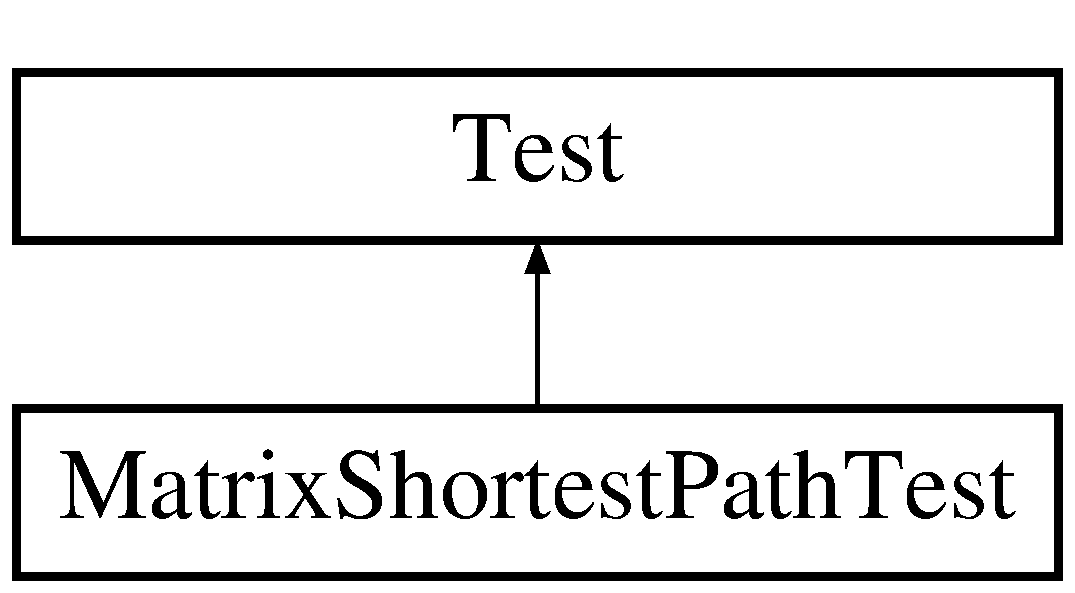
\includegraphics[height=2.000000cm]{class_matrix_shortest_path_test}
\end{center}
\end{figure}
\subsection*{Public Types}
\begin{DoxyCompactItemize}
\item 
typedef \hyperlink{struct_introduction_to_algorithm_1_1_graph_algorithm_1_1_graph}{Graph}$<$ M\+T\+\_\+\+N, \hyperlink{struct_introduction_to_algorithm_1_1_graph_algorithm_1_1_vertex}{Vertex}$<$ int $>$ $>$ \hyperlink{class_matrix_shortest_path_test_afa4c36c0b2a1b6974b44ba02e91f82ef}{G\+Type}
\end{DoxyCompactItemize}
\subsection*{Protected Member Functions}
\begin{DoxyCompactItemize}
\item 
void \hyperlink{class_matrix_shortest_path_test_ac368aa3abba1f53406aca6232ad3b45f}{Set\+Up} ()
\item 
void \hyperlink{class_matrix_shortest_path_test_a9087eff691e1d93e11c16b9ad0ed3a5d}{Tear\+Down} ()
\end{DoxyCompactItemize}
\subsection*{Protected Attributes}
\begin{DoxyCompactItemize}
\item 
std\+::shared\+\_\+ptr$<$ \hyperlink{class_matrix_shortest_path_test_afa4c36c0b2a1b6974b44ba02e91f82ef}{G\+Type} $>$ \hyperlink{class_matrix_shortest_path_test_ab574b85fb02ec6e3c737277385073a2e}{\+\_\+graph}
\end{DoxyCompactItemize}


\subsection{Detailed Description}
\hyperlink{class_matrix_shortest_path_test}{Matrix\+Shortest\+Path\+Test}\+:测试类,用于为测试提供基础数据 

{\ttfamily \hyperlink{class_matrix_shortest_path_test}{Matrix\+Shortest\+Path\+Test}}是 {\ttfamily \+::testing\+::\+Test} 的子类。它主要用于为每一个{\ttfamily T\+E\+S\+T\+\_\+\+F}准备测试环境 

Definition at line 42 of file matrix\+\_\+shortest\+\_\+path\+\_\+test.\+h.



\subsection{Member Typedef Documentation}
\hypertarget{class_matrix_shortest_path_test_afa4c36c0b2a1b6974b44ba02e91f82ef}{}\index{Matrix\+Shortest\+Path\+Test@{Matrix\+Shortest\+Path\+Test}!G\+Type@{G\+Type}}
\index{G\+Type@{G\+Type}!Matrix\+Shortest\+Path\+Test@{Matrix\+Shortest\+Path\+Test}}
\subsubsection[{G\+Type}]{\setlength{\rightskip}{0pt plus 5cm}typedef {\bf Graph}$<$M\+T\+\_\+\+N,{\bf Vertex}$<$int$>$ $>$ {\bf Matrix\+Shortest\+Path\+Test\+::\+G\+Type}}\label{class_matrix_shortest_path_test_afa4c36c0b2a1b6974b44ba02e91f82ef}
模板实例化的图类型,该图的顶点类型为{\ttfamily Vertex$<$int$>$} 

Definition at line 45 of file matrix\+\_\+shortest\+\_\+path\+\_\+test.\+h.



\subsection{Member Function Documentation}
\hypertarget{class_matrix_shortest_path_test_ac368aa3abba1f53406aca6232ad3b45f}{}\index{Matrix\+Shortest\+Path\+Test@{Matrix\+Shortest\+Path\+Test}!Set\+Up@{Set\+Up}}
\index{Set\+Up@{Set\+Up}!Matrix\+Shortest\+Path\+Test@{Matrix\+Shortest\+Path\+Test}}
\subsubsection[{Set\+Up()}]{\setlength{\rightskip}{0pt plus 5cm}void Matrix\+Shortest\+Path\+Test\+::\+Set\+Up (
\begin{DoxyParamCaption}
{}
\end{DoxyParamCaption}
)\hspace{0.3cm}{\ttfamily [inline]}, {\ttfamily [protected]}}\label{class_matrix_shortest_path_test_ac368aa3abba1f53406aca6232ad3b45f}


Definition at line 48 of file matrix\+\_\+shortest\+\_\+path\+\_\+test.\+h.

\hypertarget{class_matrix_shortest_path_test_a9087eff691e1d93e11c16b9ad0ed3a5d}{}\index{Matrix\+Shortest\+Path\+Test@{Matrix\+Shortest\+Path\+Test}!Tear\+Down@{Tear\+Down}}
\index{Tear\+Down@{Tear\+Down}!Matrix\+Shortest\+Path\+Test@{Matrix\+Shortest\+Path\+Test}}
\subsubsection[{Tear\+Down()}]{\setlength{\rightskip}{0pt plus 5cm}void Matrix\+Shortest\+Path\+Test\+::\+Tear\+Down (
\begin{DoxyParamCaption}
{}
\end{DoxyParamCaption}
)\hspace{0.3cm}{\ttfamily [inline]}, {\ttfamily [protected]}}\label{class_matrix_shortest_path_test_a9087eff691e1d93e11c16b9ad0ed3a5d}


Definition at line 66 of file matrix\+\_\+shortest\+\_\+path\+\_\+test.\+h.



\subsection{Member Data Documentation}
\hypertarget{class_matrix_shortest_path_test_ab574b85fb02ec6e3c737277385073a2e}{}\index{Matrix\+Shortest\+Path\+Test@{Matrix\+Shortest\+Path\+Test}!\+\_\+graph@{\+\_\+graph}}
\index{\+\_\+graph@{\+\_\+graph}!Matrix\+Shortest\+Path\+Test@{Matrix\+Shortest\+Path\+Test}}
\subsubsection[{\+\_\+graph}]{\setlength{\rightskip}{0pt plus 5cm}std\+::shared\+\_\+ptr$<${\bf G\+Type}$>$ Matrix\+Shortest\+Path\+Test\+::\+\_\+graph\hspace{0.3cm}{\ttfamily [protected]}}\label{class_matrix_shortest_path_test_ab574b85fb02ec6e3c737277385073a2e}
指向一个图,算法导论图25-\/1 

Definition at line 67 of file matrix\+\_\+shortest\+\_\+path\+\_\+test.\+h.



The documentation for this class was generated from the following file\+:\begin{DoxyCompactItemize}
\item 
src/graph\+\_\+algorithms/all\+\_\+node\+\_\+pair\+\_\+shortest\+\_\+path/matrix\+\_\+shortest\+\_\+path/\hyperlink{matrix__shortest__path__test_8h}{matrix\+\_\+shortest\+\_\+path\+\_\+test.\+h}\end{DoxyCompactItemize}

\hypertarget{class_introduction_to_algorithm_1_1_queue_algorithm_1_1_min_queue}{}\section{Introduction\+To\+Algorithm\+:\+:Queue\+Algorithm\+:\+:Min\+Queue$<$ T, T\+Key\+Type $>$ Class Template Reference}
\label{class_introduction_to_algorithm_1_1_queue_algorithm_1_1_min_queue}\index{Introduction\+To\+Algorithm\+::\+Queue\+Algorithm\+::\+Min\+Queue$<$ T, T\+Key\+Type $>$@{Introduction\+To\+Algorithm\+::\+Queue\+Algorithm\+::\+Min\+Queue$<$ T, T\+Key\+Type $>$}}


Min\+Queue:最小优先级队列,算法导论第6章6.5节  




{\ttfamily \#include $<$minqueue.\+h$>$}

\subsection*{Public Types}
\begin{DoxyCompactItemize}
\item 
typedef std\+::function$<$ bool(std\+::shared\+\_\+ptr$<$ T $>$, std\+::shared\+\_\+ptr$<$ T $>$)$>$ \hyperlink{class_introduction_to_algorithm_1_1_queue_algorithm_1_1_min_queue_a8f2f5b5d2b7097bbc6edda7b9c9228a6}{Compare\+Type}
\item 
typedef std\+::function$<$ T\+Key\+Type \&(std\+::shared\+\_\+ptr$<$ T $>$)$>$ \hyperlink{class_introduction_to_algorithm_1_1_queue_algorithm_1_1_min_queue_a391cb754ab172d1d4cdefd34130b917c}{Get\+Key\+Type}
\end{DoxyCompactItemize}
\subsection*{Public Member Functions}
\begin{DoxyCompactItemize}
\item 
\hyperlink{class_introduction_to_algorithm_1_1_queue_algorithm_1_1_min_queue_a98e54e4e2c19918032b09e23e79a25e5}{Min\+Queue} (\hyperlink{class_introduction_to_algorithm_1_1_queue_algorithm_1_1_min_queue_a8f2f5b5d2b7097bbc6edda7b9c9228a6}{Compare\+Type} compare, \hyperlink{class_introduction_to_algorithm_1_1_queue_algorithm_1_1_min_queue_a391cb754ab172d1d4cdefd34130b917c}{Get\+Key\+Type} get\+Key)
\begin{DoxyCompactList}\small\item\em 显式构造函数 \end{DoxyCompactList}\item 
\hyperlink{class_introduction_to_algorithm_1_1_queue_algorithm_1_1_min_queue_a770243b2227a15bdc2105dde6549c745}{Min\+Queue} (std\+::size\+\_\+t reseve\+\_\+size, \hyperlink{class_introduction_to_algorithm_1_1_queue_algorithm_1_1_min_queue_a8f2f5b5d2b7097bbc6edda7b9c9228a6}{Compare\+Type} compare, \hyperlink{class_introduction_to_algorithm_1_1_queue_algorithm_1_1_min_queue_a391cb754ab172d1d4cdefd34130b917c}{Get\+Key\+Type} get\+Key)
\begin{DoxyCompactList}\small\item\em 显式构造函数 \end{DoxyCompactList}\item 
std\+::shared\+\_\+ptr$<$ T $>$ \hyperlink{class_introduction_to_algorithm_1_1_queue_algorithm_1_1_min_queue_a96293074ee6adef713e9e47059958ea2}{min} ()
\begin{DoxyCompactList}\small\item\em min\+:返回最小值 \end{DoxyCompactList}\item 
std\+::shared\+\_\+ptr$<$ T $>$ \hyperlink{class_introduction_to_algorithm_1_1_queue_algorithm_1_1_min_queue_a71022b9e1e9993ec5c5876da9e6e6eee}{extract\+\_\+min} ()
\begin{DoxyCompactList}\small\item\em extract\+\_\+min\+:删除队列中最小值,并返回最小值 \end{DoxyCompactList}\item 
int \hyperlink{class_introduction_to_algorithm_1_1_queue_algorithm_1_1_min_queue_a0992696959d7300082654529becd1765}{insert} (std\+::shared\+\_\+ptr$<$ T $>$ element)
\begin{DoxyCompactList}\small\item\em insert\+:向队列中插入一个元素 \end{DoxyCompactList}\item 
bool \hyperlink{class_introduction_to_algorithm_1_1_queue_algorithm_1_1_min_queue_a1b484baf6cd011a4b91aa77a644e5a44}{is\+\_\+empty} ()
\begin{DoxyCompactList}\small\item\em is\+\_\+empty\+:返回队列是否为空 \end{DoxyCompactList}\item 
int \hyperlink{class_introduction_to_algorithm_1_1_queue_algorithm_1_1_min_queue_a545dbdb76e0b6e9c4227e558ab9b1239}{index\+\_\+inqueue} (std\+::shared\+\_\+ptr$<$ T $>$ element)
\begin{DoxyCompactList}\small\item\em is\+\_\+inqueue\+:返回指定元素是否在队列中 \end{DoxyCompactList}\item 
void \hyperlink{class_introduction_to_algorithm_1_1_queue_algorithm_1_1_min_queue_aa934049abcfedd59fa9ffe6d91fea30c}{decreate\+\_\+key} (std\+::size\+\_\+t element\+\_\+index, T\+Key\+Type new\+\_\+key)
\begin{DoxyCompactList}\small\item\em decreate\+\_\+key\+:缩减队列中某个元素的{\ttfamily key} \end{DoxyCompactList}\item 
void \hyperlink{class_introduction_to_algorithm_1_1_queue_algorithm_1_1_min_queue_a9a432c7c167a4f9a56c2988cfdc04620}{setup\+Heap} ()
\begin{DoxyCompactList}\small\item\em setup\+Heap\+:建堆 \end{DoxyCompactList}\item 
void \hyperlink{class_introduction_to_algorithm_1_1_queue_algorithm_1_1_min_queue_a4ddfab80f781d5b5f7544164bf266f82}{heapify} (std\+::size\+\_\+t element\+Index)
\begin{DoxyCompactList}\small\item\em heapify:维持堆性质 \end{DoxyCompactList}\end{DoxyCompactItemize}
\subsection*{Protected Member Functions}
\begin{DoxyCompactItemize}
\item 
std\+::size\+\_\+t \hyperlink{class_introduction_to_algorithm_1_1_queue_algorithm_1_1_min_queue_a3b7cac401c8cf45806e61aad3799eda0}{\+\_\+parent\+Index} (std\+::size\+\_\+t element\+Index, bool \&valid)
\begin{DoxyCompactList}\small\item\em \+\_\+parent\+Index\+:返回一个节点的父节点位置 \end{DoxyCompactList}\item 
std\+::size\+\_\+t \hyperlink{class_introduction_to_algorithm_1_1_queue_algorithm_1_1_min_queue_a0d2a517cd63fc33c0403a4d4c83c7e9d}{\+\_\+lchild\+Index} (std\+::size\+\_\+t element\+Index, bool \&valid)
\begin{DoxyCompactList}\small\item\em \+\_\+lchild\+Index\+:返回一个节点的左子节点位置 \end{DoxyCompactList}\item 
std\+::size\+\_\+t \hyperlink{class_introduction_to_algorithm_1_1_queue_algorithm_1_1_min_queue_a7129becd0fd74b5d2c17702e65f32300}{\+\_\+rchild\+Index} (std\+::size\+\_\+t element\+Index, bool \&valid)
\begin{DoxyCompactList}\small\item\em \+\_\+rchild\+Index\+:返回一个节点的右子节点位置 \end{DoxyCompactList}\end{DoxyCompactItemize}
\subsection*{Private Attributes}
\begin{DoxyCompactItemize}
\item 
std\+::vector$<$ std\+::shared\+\_\+ptr$<$ T $>$ $>$ \hyperlink{class_introduction_to_algorithm_1_1_queue_algorithm_1_1_min_queue_ad463395cef741624e6d078e4e4fc624f}{\+\_\+data}
\item 
std\+::size\+\_\+t \hyperlink{class_introduction_to_algorithm_1_1_queue_algorithm_1_1_min_queue_a0de92802e37516dda2c01de776aba641}{\+\_\+size}
\item 
\hyperlink{class_introduction_to_algorithm_1_1_queue_algorithm_1_1_min_queue_a8f2f5b5d2b7097bbc6edda7b9c9228a6}{Compare\+Type} \hyperlink{class_introduction_to_algorithm_1_1_queue_algorithm_1_1_min_queue_a5de60762d317fc92c18e882dd50f8dfa}{\+\_\+compare}
\item 
\hyperlink{class_introduction_to_algorithm_1_1_queue_algorithm_1_1_min_queue_a391cb754ab172d1d4cdefd34130b917c}{Get\+Key\+Type} \hyperlink{class_introduction_to_algorithm_1_1_queue_algorithm_1_1_min_queue_a3f791f9dd9d61dc2caf1d6b2b354f4c4}{\+\_\+get\+Key}
\end{DoxyCompactItemize}


\subsection{Detailed Description}
\subsubsection*{template$<$typename T, typename T\+Key\+Type$>$class Introduction\+To\+Algorithm\+::\+Queue\+Algorithm\+::\+Min\+Queue$<$ T, T\+Key\+Type $>$}

Min\+Queue:最小优先级队列,算法导论第6章6.5节 

优先级队列是一种用来维护由一组元素构成集合\+S的数据结构,其中每个元素都有一个相关的值,称之为关键字。一个最小优先级队列支持以下操作:


\begin{DoxyItemize}
\item insert(\+S,x)\+:将元素x插入到集合\+S中。
\item min(\+S)\+:返回\+S中具有最小关键字的元素
\item extract\+\_\+min(\+S)\+:去掉并返回\+S中具有最小关键字的元素
\item decrease\+\_\+key(\+S,x,k)\+:将元素x的关键字值减小到k,这里要求k的值小于x的原始关键字
\end{DoxyItemize}

本算法的实现时,有以下几种变化:


\begin{DoxyItemize}
\item 增加了以下的接口:
\begin{DoxyItemize}
\item is\+\_\+empty(\+S)\+: 返回\+S是否为空
\item is\+\_\+inqueue(\+S,x)\+:判断元素x是否在\+S中
\item setup\+Heap(\+S)\+:建立最小堆(由堆的接口遗留而来)
\item heapify(\+S,index)\+:操作堆的指定结点使得它符合最小堆条件(由堆的接口遗留下来)
\end{DoxyItemize}
\item 增加了队列容量属性。队列容量由{\ttfamily \+\_\+data}的大小来表征。默认将{\ttfamily \+\_\+data}大小设为0;可以显式提供{\ttfamily reseve\+\_\+size}参数来设置{\ttfamily \+\_\+data}的大小。 队列容量用于限制队列大小。一旦队列已满,则下一次插入之前会将队列容量增加一倍;一旦队列不足队列的1/4,则一旦执行{\ttfamily extract\+\_\+min}操作则将队列容量缩减至一半
\item 增加了两个特殊的可调用对象,这两个方法的引入使得最小优先级队列不仅可以应用于class和struct类型,也可以应用于int,double等非类的类型
\begin{DoxyItemize}
\item \+\_\+get\+Key\+:是一个std\+:\+:function$<$T\+Key\+Type\&(std\+::shared\+\_\+ptr$<$\+T$>$)$>$类型的对象,它可以接收std\+::shared\+\_\+ptr$<$\+T$>$类型的参数,返回\+T\+Key\+Type类型的引用。 其中队列保存的是\+T类型数据的强引用,\+T\+Key\+Type是\+T类型数据的关键字类型。通过\+\_\+get\+Key可以获取队列数据的关键字的引用。
\begin{DoxyItemize}
\item 对于class类型,\+T\+Key\+Type就是\+T对象的关键字类型,\+\_\+get\+Key就是返回关键字的引用
\item 对于int等内置类型,\+T\+Key\+Type就是\+T本身。\+\_\+get\+Key就是返回它自身的引用
\end{DoxyItemize}
\item \+\_\+compare\+:是一个std\+:\+:function$<$bool (std\+::shared\+\_\+ptr$<$\+T$>$,std\+::shared\+\_\+ptr$<$\+T$>$)$>$类型的对象,它用于队列中两个数据的大小比较。 
\end{DoxyItemize}
\end{DoxyItemize}

Definition at line 60 of file minqueue.\+h.



\subsection{Member Typedef Documentation}
\hypertarget{class_introduction_to_algorithm_1_1_queue_algorithm_1_1_min_queue_a8f2f5b5d2b7097bbc6edda7b9c9228a6}{}\index{Introduction\+To\+Algorithm\+::\+Queue\+Algorithm\+::\+Min\+Queue@{Introduction\+To\+Algorithm\+::\+Queue\+Algorithm\+::\+Min\+Queue}!Compare\+Type@{Compare\+Type}}
\index{Compare\+Type@{Compare\+Type}!Introduction\+To\+Algorithm\+::\+Queue\+Algorithm\+::\+Min\+Queue@{Introduction\+To\+Algorithm\+::\+Queue\+Algorithm\+::\+Min\+Queue}}
\subsubsection[{Compare\+Type}]{\setlength{\rightskip}{0pt plus 5cm}template$<$typename T, typename T\+Key\+Type$>$ typedef std\+::function$<$bool (std\+::shared\+\_\+ptr$<$T$>$,std\+::shared\+\_\+ptr$<$T$>$)$>$ {\bf Introduction\+To\+Algorithm\+::\+Queue\+Algorithm\+::\+Min\+Queue}$<$ T, T\+Key\+Type $>$\+::{\bf Compare\+Type}}\label{class_introduction_to_algorithm_1_1_queue_algorithm_1_1_min_queue_a8f2f5b5d2b7097bbc6edda7b9c9228a6}
一个可调用对象类型,该类型的对象可用于比较两个std\+::shared\+\_\+ptr$<$\+T$>$的小于比较 

Definition at line 63 of file minqueue.\+h.

\hypertarget{class_introduction_to_algorithm_1_1_queue_algorithm_1_1_min_queue_a391cb754ab172d1d4cdefd34130b917c}{}\index{Introduction\+To\+Algorithm\+::\+Queue\+Algorithm\+::\+Min\+Queue@{Introduction\+To\+Algorithm\+::\+Queue\+Algorithm\+::\+Min\+Queue}!Get\+Key\+Type@{Get\+Key\+Type}}
\index{Get\+Key\+Type@{Get\+Key\+Type}!Introduction\+To\+Algorithm\+::\+Queue\+Algorithm\+::\+Min\+Queue@{Introduction\+To\+Algorithm\+::\+Queue\+Algorithm\+::\+Min\+Queue}}
\subsubsection[{Get\+Key\+Type}]{\setlength{\rightskip}{0pt plus 5cm}template$<$typename T, typename T\+Key\+Type$>$ typedef std\+::function$<$T\+Key\+Type\&(std\+::shared\+\_\+ptr$<$T$>$)$>$ {\bf Introduction\+To\+Algorithm\+::\+Queue\+Algorithm\+::\+Min\+Queue}$<$ T, T\+Key\+Type $>$\+::{\bf Get\+Key\+Type}}\label{class_introduction_to_algorithm_1_1_queue_algorithm_1_1_min_queue_a391cb754ab172d1d4cdefd34130b917c}
一个可调用对象,该类型的对象可用于获取std\+::shared\+\_\+ptr$<$\+T$>$的关键字,并修改该关键字(返回的是关键字的引用) 

Definition at line 64 of file minqueue.\+h.



\subsection{Constructor \& Destructor Documentation}
\hypertarget{class_introduction_to_algorithm_1_1_queue_algorithm_1_1_min_queue_a98e54e4e2c19918032b09e23e79a25e5}{}\index{Introduction\+To\+Algorithm\+::\+Queue\+Algorithm\+::\+Min\+Queue@{Introduction\+To\+Algorithm\+::\+Queue\+Algorithm\+::\+Min\+Queue}!Min\+Queue@{Min\+Queue}}
\index{Min\+Queue@{Min\+Queue}!Introduction\+To\+Algorithm\+::\+Queue\+Algorithm\+::\+Min\+Queue@{Introduction\+To\+Algorithm\+::\+Queue\+Algorithm\+::\+Min\+Queue}}
\subsubsection[{Min\+Queue(\+Compare\+Type compare, Get\+Key\+Type get\+Key)}]{\setlength{\rightskip}{0pt plus 5cm}template$<$typename T, typename T\+Key\+Type$>$ {\bf Introduction\+To\+Algorithm\+::\+Queue\+Algorithm\+::\+Min\+Queue}$<$ T, T\+Key\+Type $>$\+::{\bf Min\+Queue} (
\begin{DoxyParamCaption}
\item[{{\bf Compare\+Type}}]{compare, }
\item[{{\bf Get\+Key\+Type}}]{get\+Key}
\end{DoxyParamCaption}
)\hspace{0.3cm}{\ttfamily [inline]}}\label{class_introduction_to_algorithm_1_1_queue_algorithm_1_1_min_queue_a98e54e4e2c19918032b09e23e79a25e5}


显式构造函数 


\begin{DoxyParams}{Parameters}
{\em compare\+:一个可调用对象,可用于比较两个std\+::shared\+\_\+ptr$<$\+T$>$对象的小于比较} & \\
\hline
{\em get\+Key:一个可调用对象,它的参数为std\+::shared\+\_\+ptr$<$\+T$>$,返回\+T\+Key\&。通过它的返回值可以获取\+T的key,也可以修改\+T的key} & \\
\hline
\end{DoxyParams}


Definition at line 71 of file minqueue.\+h.

\hypertarget{class_introduction_to_algorithm_1_1_queue_algorithm_1_1_min_queue_a770243b2227a15bdc2105dde6549c745}{}\index{Introduction\+To\+Algorithm\+::\+Queue\+Algorithm\+::\+Min\+Queue@{Introduction\+To\+Algorithm\+::\+Queue\+Algorithm\+::\+Min\+Queue}!Min\+Queue@{Min\+Queue}}
\index{Min\+Queue@{Min\+Queue}!Introduction\+To\+Algorithm\+::\+Queue\+Algorithm\+::\+Min\+Queue@{Introduction\+To\+Algorithm\+::\+Queue\+Algorithm\+::\+Min\+Queue}}
\subsubsection[{Min\+Queue(std\+::size\+\_\+t reseve\+\_\+size, Compare\+Type compare, Get\+Key\+Type get\+Key)}]{\setlength{\rightskip}{0pt plus 5cm}template$<$typename T, typename T\+Key\+Type$>$ {\bf Introduction\+To\+Algorithm\+::\+Queue\+Algorithm\+::\+Min\+Queue}$<$ T, T\+Key\+Type $>$\+::{\bf Min\+Queue} (
\begin{DoxyParamCaption}
\item[{std\+::size\+\_\+t}]{reseve\+\_\+size, }
\item[{{\bf Compare\+Type}}]{compare, }
\item[{{\bf Get\+Key\+Type}}]{get\+Key}
\end{DoxyParamCaption}
)\hspace{0.3cm}{\ttfamily [inline]}}\label{class_introduction_to_algorithm_1_1_queue_algorithm_1_1_min_queue_a770243b2227a15bdc2105dde6549c745}


显式构造函数 


\begin{DoxyParams}{Parameters}
{\em reseve\+\_\+size\+:指定队列的初始容量} & \\
\hline
{\em compare\+:一个可调用对象,可用于比较两个std\+::shared\+\_\+ptr$<$\+T$>$对象的小于比较} & \\
\hline
{\em get\+Key:一个可调用对象,它的参数为std\+::shared\+\_\+ptr$<$\+T$>$,返回\+T\+Key\&。通过它的返回值可以获取\+T的key,也可以修改\+T的key} & \\
\hline
\end{DoxyParams}


Definition at line 79 of file minqueue.\+h.



\subsection{Member Function Documentation}
\hypertarget{class_introduction_to_algorithm_1_1_queue_algorithm_1_1_min_queue_a0d2a517cd63fc33c0403a4d4c83c7e9d}{}\index{Introduction\+To\+Algorithm\+::\+Queue\+Algorithm\+::\+Min\+Queue@{Introduction\+To\+Algorithm\+::\+Queue\+Algorithm\+::\+Min\+Queue}!\+\_\+lchild\+Index@{\+\_\+lchild\+Index}}
\index{\+\_\+lchild\+Index@{\+\_\+lchild\+Index}!Introduction\+To\+Algorithm\+::\+Queue\+Algorithm\+::\+Min\+Queue@{Introduction\+To\+Algorithm\+::\+Queue\+Algorithm\+::\+Min\+Queue}}
\subsubsection[{\+\_\+lchild\+Index(std\+::size\+\_\+t element\+Index, bool \&valid)}]{\setlength{\rightskip}{0pt plus 5cm}template$<$typename T, typename T\+Key\+Type$>$ std\+::size\+\_\+t {\bf Introduction\+To\+Algorithm\+::\+Queue\+Algorithm\+::\+Min\+Queue}$<$ T, T\+Key\+Type $>$\+::\+\_\+lchild\+Index (
\begin{DoxyParamCaption}
\item[{std\+::size\+\_\+t}]{element\+Index, }
\item[{bool \&}]{valid}
\end{DoxyParamCaption}
)\hspace{0.3cm}{\ttfamily [inline]}, {\ttfamily [protected]}}\label{class_introduction_to_algorithm_1_1_queue_algorithm_1_1_min_queue_a0d2a517cd63fc33c0403a4d4c83c7e9d}


\+\_\+lchild\+Index\+:返回一个节点的左子节点位置 


\begin{DoxyParams}{Parameters}
{\em element\+Index} & \+: 节点位置 \\
\hline
{\em valid} & 一个bool\&值,用于返回,指示子节点是否有效 \\
\hline
\end{DoxyParams}
\begin{DoxyReturn}{Returns}
左子节点位置(std\+::size\+\_\+t)
\end{DoxyReturn}
根据最小堆的性质,一个节点element\+Index的左子节点是它的位置(element\+Index/2)+1


\begin{DoxyItemize}
\item 当最小堆大小为0、1时,它没有左子节点,左子节点无效
\item 当左子节点超过堆大小时,它无效 
\end{DoxyItemize}

Definition at line 326 of file minqueue.\+h.

\hypertarget{class_introduction_to_algorithm_1_1_queue_algorithm_1_1_min_queue_a3b7cac401c8cf45806e61aad3799eda0}{}\index{Introduction\+To\+Algorithm\+::\+Queue\+Algorithm\+::\+Min\+Queue@{Introduction\+To\+Algorithm\+::\+Queue\+Algorithm\+::\+Min\+Queue}!\+\_\+parent\+Index@{\+\_\+parent\+Index}}
\index{\+\_\+parent\+Index@{\+\_\+parent\+Index}!Introduction\+To\+Algorithm\+::\+Queue\+Algorithm\+::\+Min\+Queue@{Introduction\+To\+Algorithm\+::\+Queue\+Algorithm\+::\+Min\+Queue}}
\subsubsection[{\+\_\+parent\+Index(std\+::size\+\_\+t element\+Index, bool \&valid)}]{\setlength{\rightskip}{0pt plus 5cm}template$<$typename T, typename T\+Key\+Type$>$ std\+::size\+\_\+t {\bf Introduction\+To\+Algorithm\+::\+Queue\+Algorithm\+::\+Min\+Queue}$<$ T, T\+Key\+Type $>$\+::\+\_\+parent\+Index (
\begin{DoxyParamCaption}
\item[{std\+::size\+\_\+t}]{element\+Index, }
\item[{bool \&}]{valid}
\end{DoxyParamCaption}
)\hspace{0.3cm}{\ttfamily [inline]}, {\ttfamily [protected]}}\label{class_introduction_to_algorithm_1_1_queue_algorithm_1_1_min_queue_a3b7cac401c8cf45806e61aad3799eda0}


\+\_\+parent\+Index\+:返回一个节点的父节点位置 


\begin{DoxyParams}{Parameters}
{\em element\+Index} & \+: 子节点位置 \\
\hline
{\em valid} & 一个bool\&值,用于返回,指示父节点是否有效 \\
\hline
\end{DoxyParams}
\begin{DoxyReturn}{Returns}
父节点位置(std\+::size\+\_\+t)
\end{DoxyReturn}
根据最小堆的性质,一个子节点element\+Index的父节点是它的位置(element\+Index-\/1)/2。


\begin{DoxyItemize}
\item 超出堆大小的节点,其父节点无效 
\end{DoxyItemize}

Definition at line 303 of file minqueue.\+h.

\hypertarget{class_introduction_to_algorithm_1_1_queue_algorithm_1_1_min_queue_a7129becd0fd74b5d2c17702e65f32300}{}\index{Introduction\+To\+Algorithm\+::\+Queue\+Algorithm\+::\+Min\+Queue@{Introduction\+To\+Algorithm\+::\+Queue\+Algorithm\+::\+Min\+Queue}!\+\_\+rchild\+Index@{\+\_\+rchild\+Index}}
\index{\+\_\+rchild\+Index@{\+\_\+rchild\+Index}!Introduction\+To\+Algorithm\+::\+Queue\+Algorithm\+::\+Min\+Queue@{Introduction\+To\+Algorithm\+::\+Queue\+Algorithm\+::\+Min\+Queue}}
\subsubsection[{\+\_\+rchild\+Index(std\+::size\+\_\+t element\+Index, bool \&valid)}]{\setlength{\rightskip}{0pt plus 5cm}template$<$typename T, typename T\+Key\+Type$>$ std\+::size\+\_\+t {\bf Introduction\+To\+Algorithm\+::\+Queue\+Algorithm\+::\+Min\+Queue}$<$ T, T\+Key\+Type $>$\+::\+\_\+rchild\+Index (
\begin{DoxyParamCaption}
\item[{std\+::size\+\_\+t}]{element\+Index, }
\item[{bool \&}]{valid}
\end{DoxyParamCaption}
)\hspace{0.3cm}{\ttfamily [inline]}, {\ttfamily [protected]}}\label{class_introduction_to_algorithm_1_1_queue_algorithm_1_1_min_queue_a7129becd0fd74b5d2c17702e65f32300}


\+\_\+rchild\+Index\+:返回一个节点的右子节点位置 


\begin{DoxyParams}{Parameters}
{\em element\+Index} & \+: 节点位置 \\
\hline
{\em valid} & 一个bool\&值,用于返回,指示子节点是否有效 \\
\hline
\end{DoxyParams}
\begin{DoxyReturn}{Returns}
右子节点位置(std\+::size\+\_\+t)
\end{DoxyReturn}
根据最小堆的性质,一个节点element\+Index的右子节点是它的位置(element\+Index/2)+2


\begin{DoxyItemize}
\item 当最小堆大小为0、、1、2时,它没有右子节点,右子节点无效
\item 当右子节点超过堆大小时,它无效 
\end{DoxyItemize}

Definition at line 353 of file minqueue.\+h.

\hypertarget{class_introduction_to_algorithm_1_1_queue_algorithm_1_1_min_queue_aa934049abcfedd59fa9ffe6d91fea30c}{}\index{Introduction\+To\+Algorithm\+::\+Queue\+Algorithm\+::\+Min\+Queue@{Introduction\+To\+Algorithm\+::\+Queue\+Algorithm\+::\+Min\+Queue}!decreate\+\_\+key@{decreate\+\_\+key}}
\index{decreate\+\_\+key@{decreate\+\_\+key}!Introduction\+To\+Algorithm\+::\+Queue\+Algorithm\+::\+Min\+Queue@{Introduction\+To\+Algorithm\+::\+Queue\+Algorithm\+::\+Min\+Queue}}
\subsubsection[{decreate\+\_\+key(std\+::size\+\_\+t element\+\_\+index, T\+Key\+Type new\+\_\+key)}]{\setlength{\rightskip}{0pt plus 5cm}template$<$typename T, typename T\+Key\+Type$>$ void {\bf Introduction\+To\+Algorithm\+::\+Queue\+Algorithm\+::\+Min\+Queue}$<$ T, T\+Key\+Type $>$\+::decreate\+\_\+key (
\begin{DoxyParamCaption}
\item[{std\+::size\+\_\+t}]{element\+\_\+index, }
\item[{T\+Key\+Type}]{new\+\_\+key}
\end{DoxyParamCaption}
)\hspace{0.3cm}{\ttfamily [inline]}}\label{class_introduction_to_algorithm_1_1_queue_algorithm_1_1_min_queue_aa934049abcfedd59fa9ffe6d91fea30c}


decreate\+\_\+key\+:缩减队列中某个元素的{\ttfamily key} 


\begin{DoxyParams}{Parameters}
{\em element\+\_\+index} & 待缩减元素的下标 \\
\hline
{\em new\+\_\+key:待缩减元素的新$<$tt$>$key$<$/tt$>$,类型为\+T\+Key} & 缩减之前先判断缩减是否有效,若无效则抛出异常。\\
\hline
\end{DoxyParams}

\begin{DoxyItemize}
\item 若{\ttfamily element\+\_\+index}超过了队列大小,则抛出异常
\item 若{\ttfamily new\+\_\+key}大于等于待缩减元素的{\ttfamily key},则抛出异常
\end{DoxyItemize}

缩减过程为:


\begin{DoxyItemize}
\item 将待缩减元素的{\ttfamily key}赋值为新值
\item 不断的将该元素向父节点比较:
\begin{DoxyItemize}
\item 若父节点较小,则终止比较过程
\item 若父节点较大,则交换当前节点与父节点,并将当前节点指向父节点进行下一轮比较
\item 若当前节点已经是队列首个元素,则终止比较过程
\end{DoxyItemize}
\item 时间复杂度 O(h)
\item 原地操作 
\end{DoxyItemize}

Definition at line 216 of file minqueue.\+h.

\hypertarget{class_introduction_to_algorithm_1_1_queue_algorithm_1_1_min_queue_a71022b9e1e9993ec5c5876da9e6e6eee}{}\index{Introduction\+To\+Algorithm\+::\+Queue\+Algorithm\+::\+Min\+Queue@{Introduction\+To\+Algorithm\+::\+Queue\+Algorithm\+::\+Min\+Queue}!extract\+\_\+min@{extract\+\_\+min}}
\index{extract\+\_\+min@{extract\+\_\+min}!Introduction\+To\+Algorithm\+::\+Queue\+Algorithm\+::\+Min\+Queue@{Introduction\+To\+Algorithm\+::\+Queue\+Algorithm\+::\+Min\+Queue}}
\subsubsection[{extract\+\_\+min()}]{\setlength{\rightskip}{0pt plus 5cm}template$<$typename T, typename T\+Key\+Type$>$ std\+::shared\+\_\+ptr$<$T$>$ {\bf Introduction\+To\+Algorithm\+::\+Queue\+Algorithm\+::\+Min\+Queue}$<$ T, T\+Key\+Type $>$\+::extract\+\_\+min (
\begin{DoxyParamCaption}
{}
\end{DoxyParamCaption}
)\hspace{0.3cm}{\ttfamily [inline]}}\label{class_introduction_to_algorithm_1_1_queue_algorithm_1_1_min_queue_a71022b9e1e9993ec5c5876da9e6e6eee}


extract\+\_\+min\+:删除队列中最小值,并返回最小值 

\begin{DoxyReturn}{Returns}
最小值的强引用
\end{DoxyReturn}
根据最小堆的性质,队列的第一个值就是最小值的强引用。


\begin{DoxyItemize}
\item 如果队列为空,则返回一个空引用
\item 如果队列非空,则执行以下操作:
\begin{DoxyItemize}
\item 交换队列的第一个元素和最后一个元素
\item 队列的{\ttfamily \+\_\+size}自减
\item 此时队列的首个元素违反了最小堆性质,因此执行{\ttfamily heapify(0)}保持性质
\item 返回旧的首个元素
\end{DoxyItemize}
\end{DoxyItemize}

一旦队列长度不足容量的1/4,则将队列容量设置为队列长度的一倍(为了防止极端情况,如\+\_\+size=0,此时将队列容量设为队列长度的一倍加上2)


\begin{DoxyItemize}
\item 时间复杂度 O(h),h为堆的高度
\item 原地操作 
\end{DoxyItemize}

Definition at line 116 of file minqueue.\+h.

\hypertarget{class_introduction_to_algorithm_1_1_queue_algorithm_1_1_min_queue_a4ddfab80f781d5b5f7544164bf266f82}{}\index{Introduction\+To\+Algorithm\+::\+Queue\+Algorithm\+::\+Min\+Queue@{Introduction\+To\+Algorithm\+::\+Queue\+Algorithm\+::\+Min\+Queue}!heapify@{heapify}}
\index{heapify@{heapify}!Introduction\+To\+Algorithm\+::\+Queue\+Algorithm\+::\+Min\+Queue@{Introduction\+To\+Algorithm\+::\+Queue\+Algorithm\+::\+Min\+Queue}}
\subsubsection[{heapify(std\+::size\+\_\+t element\+Index)}]{\setlength{\rightskip}{0pt plus 5cm}template$<$typename T, typename T\+Key\+Type$>$ void {\bf Introduction\+To\+Algorithm\+::\+Queue\+Algorithm\+::\+Min\+Queue}$<$ T, T\+Key\+Type $>$\+::heapify (
\begin{DoxyParamCaption}
\item[{std\+::size\+\_\+t}]{element\+Index}
\end{DoxyParamCaption}
)\hspace{0.3cm}{\ttfamily [inline]}}\label{class_introduction_to_algorithm_1_1_queue_algorithm_1_1_min_queue_a4ddfab80f781d5b5f7544164bf266f82}


heapify:维持堆性质 


\begin{DoxyParams}{Parameters}
{\em element\+Index} & \+: 要维持以该节点为根节点的子堆的堆性质 \\
\hline
\end{DoxyParams}
\begin{DoxyReturn}{Returns}
void
\end{DoxyReturn}
首先调用比较该节点与左右子节点的最小值。如果最小值为它本身,则维持了性质,返回;如果最小值不是它本身,那么必然为左、右子节点之一。 将该最小节点(假设为左子节点)交换到根节点,然后以左子节点递归调用heapify操作


\begin{DoxyItemize}
\item 时间复杂度 O(n)
\item 原地操作 
\end{DoxyItemize}

Definition at line 265 of file minqueue.\+h.

\hypertarget{class_introduction_to_algorithm_1_1_queue_algorithm_1_1_min_queue_a545dbdb76e0b6e9c4227e558ab9b1239}{}\index{Introduction\+To\+Algorithm\+::\+Queue\+Algorithm\+::\+Min\+Queue@{Introduction\+To\+Algorithm\+::\+Queue\+Algorithm\+::\+Min\+Queue}!index\+\_\+inqueue@{index\+\_\+inqueue}}
\index{index\+\_\+inqueue@{index\+\_\+inqueue}!Introduction\+To\+Algorithm\+::\+Queue\+Algorithm\+::\+Min\+Queue@{Introduction\+To\+Algorithm\+::\+Queue\+Algorithm\+::\+Min\+Queue}}
\subsubsection[{index\+\_\+inqueue(std\+::shared\+\_\+ptr$<$ T $>$ element)}]{\setlength{\rightskip}{0pt plus 5cm}template$<$typename T, typename T\+Key\+Type$>$ int {\bf Introduction\+To\+Algorithm\+::\+Queue\+Algorithm\+::\+Min\+Queue}$<$ T, T\+Key\+Type $>$\+::index\+\_\+inqueue (
\begin{DoxyParamCaption}
\item[{std\+::shared\+\_\+ptr$<$ T $>$}]{element}
\end{DoxyParamCaption}
)\hspace{0.3cm}{\ttfamily [inline]}}\label{class_introduction_to_algorithm_1_1_queue_algorithm_1_1_min_queue_a545dbdb76e0b6e9c4227e558ab9b1239}


is\+\_\+inqueue\+:返回指定元素是否在队列中 


\begin{DoxyParams}{Parameters}
{\em element\+:待判定的元素,要求非空。若它为空引用则抛出异常} & \\
\hline
\end{DoxyParams}
\begin{DoxyReturn}{Returns}
指定元素在队列中的下标
\end{DoxyReturn}
从前到后依次遍历队列,如果队列中某个元素等于{\ttfamily element},则返回非负整数值, 代表它在队列的std\+::vector中的位置;否则返回-\/1


\begin{DoxyItemize}
\item 时间复杂度 O(h) 
\end{DoxyItemize}

Definition at line 185 of file minqueue.\+h.

\hypertarget{class_introduction_to_algorithm_1_1_queue_algorithm_1_1_min_queue_a0992696959d7300082654529becd1765}{}\index{Introduction\+To\+Algorithm\+::\+Queue\+Algorithm\+::\+Min\+Queue@{Introduction\+To\+Algorithm\+::\+Queue\+Algorithm\+::\+Min\+Queue}!insert@{insert}}
\index{insert@{insert}!Introduction\+To\+Algorithm\+::\+Queue\+Algorithm\+::\+Min\+Queue@{Introduction\+To\+Algorithm\+::\+Queue\+Algorithm\+::\+Min\+Queue}}
\subsubsection[{insert(std\+::shared\+\_\+ptr$<$ T $>$ element)}]{\setlength{\rightskip}{0pt plus 5cm}template$<$typename T, typename T\+Key\+Type$>$ int {\bf Introduction\+To\+Algorithm\+::\+Queue\+Algorithm\+::\+Min\+Queue}$<$ T, T\+Key\+Type $>$\+::insert (
\begin{DoxyParamCaption}
\item[{std\+::shared\+\_\+ptr$<$ T $>$}]{element}
\end{DoxyParamCaption}
)\hspace{0.3cm}{\ttfamily [inline]}}\label{class_introduction_to_algorithm_1_1_queue_algorithm_1_1_min_queue_a0992696959d7300082654529becd1765}


insert\+:向队列中插入一个元素 


\begin{DoxyParams}{Parameters}
{\em element} & 待插入元素,如果元素为空引用则直接返回 \\
\hline
\end{DoxyParams}
\begin{DoxyReturn}{Returns}
\+: 插入的元素在队列中的位置。若元素为空指针则返回-\/1
\end{DoxyReturn}
插入之前首先判断队列是否已满。若队列已满,则将{\ttfamily \+\_\+data}扩容为大小{\ttfamily \+\_\+size$\ast$2+2}。


\begin{DoxyItemize}
\item 若{\ttfamily \+\_\+size==\+\_\+data.\+size()}则说明队列已满
\end{DoxyItemize}

插入过程为:


\begin{DoxyItemize}
\item 保留待插入元素的{\ttfamily key},同时将待插入语元素的{\ttfamily key}设置为无穷大,并将待插入元素插入到队尾
\item 执行{\ttfamily decreate\+\_\+key(..)}操作
\end{DoxyItemize}

一旦队列已满,则将队列容量设置为队列长度的一倍(为了防止极端情况,如\+\_\+size=0,此时将队列容量设为队列长度的一倍加上2)


\begin{DoxyItemize}
\item 时间复杂度 O(h)
\item 原地操作 
\end{DoxyItemize}

Definition at line 148 of file minqueue.\+h.

\hypertarget{class_introduction_to_algorithm_1_1_queue_algorithm_1_1_min_queue_a1b484baf6cd011a4b91aa77a644e5a44}{}\index{Introduction\+To\+Algorithm\+::\+Queue\+Algorithm\+::\+Min\+Queue@{Introduction\+To\+Algorithm\+::\+Queue\+Algorithm\+::\+Min\+Queue}!is\+\_\+empty@{is\+\_\+empty}}
\index{is\+\_\+empty@{is\+\_\+empty}!Introduction\+To\+Algorithm\+::\+Queue\+Algorithm\+::\+Min\+Queue@{Introduction\+To\+Algorithm\+::\+Queue\+Algorithm\+::\+Min\+Queue}}
\subsubsection[{is\+\_\+empty()}]{\setlength{\rightskip}{0pt plus 5cm}template$<$typename T, typename T\+Key\+Type$>$ bool {\bf Introduction\+To\+Algorithm\+::\+Queue\+Algorithm\+::\+Min\+Queue}$<$ T, T\+Key\+Type $>$\+::is\+\_\+empty (
\begin{DoxyParamCaption}
{}
\end{DoxyParamCaption}
)\hspace{0.3cm}{\ttfamily [inline]}}\label{class_introduction_to_algorithm_1_1_queue_algorithm_1_1_min_queue_a1b484baf6cd011a4b91aa77a644e5a44}


is\+\_\+empty\+:返回队列是否为空 

\begin{DoxyReturn}{Returns}
队列是否为空
\end{DoxyReturn}
若队列的{\ttfamily \+\_\+size}为0,则队列为空;否则队列不为空


\begin{DoxyItemize}
\item 时间复杂度 O(1) 
\end{DoxyItemize}

Definition at line 170 of file minqueue.\+h.

\hypertarget{class_introduction_to_algorithm_1_1_queue_algorithm_1_1_min_queue_a96293074ee6adef713e9e47059958ea2}{}\index{Introduction\+To\+Algorithm\+::\+Queue\+Algorithm\+::\+Min\+Queue@{Introduction\+To\+Algorithm\+::\+Queue\+Algorithm\+::\+Min\+Queue}!min@{min}}
\index{min@{min}!Introduction\+To\+Algorithm\+::\+Queue\+Algorithm\+::\+Min\+Queue@{Introduction\+To\+Algorithm\+::\+Queue\+Algorithm\+::\+Min\+Queue}}
\subsubsection[{min()}]{\setlength{\rightskip}{0pt plus 5cm}template$<$typename T, typename T\+Key\+Type$>$ std\+::shared\+\_\+ptr$<$T$>$ {\bf Introduction\+To\+Algorithm\+::\+Queue\+Algorithm\+::\+Min\+Queue}$<$ T, T\+Key\+Type $>$\+::min (
\begin{DoxyParamCaption}
{}
\end{DoxyParamCaption}
)\hspace{0.3cm}{\ttfamily [inline]}}\label{class_introduction_to_algorithm_1_1_queue_algorithm_1_1_min_queue_a96293074ee6adef713e9e47059958ea2}


min\+:返回最小值 

\begin{DoxyReturn}{Returns}
最小值的强引用
\end{DoxyReturn}
根据最小堆的性质,队列的第一个值就是最小值的强引用。如果队列为空,则返回一个空引用


\begin{DoxyItemize}
\item 时间复杂度 O(1) 
\end{DoxyItemize}

Definition at line 92 of file minqueue.\+h.

\hypertarget{class_introduction_to_algorithm_1_1_queue_algorithm_1_1_min_queue_a9a432c7c167a4f9a56c2988cfdc04620}{}\index{Introduction\+To\+Algorithm\+::\+Queue\+Algorithm\+::\+Min\+Queue@{Introduction\+To\+Algorithm\+::\+Queue\+Algorithm\+::\+Min\+Queue}!setup\+Heap@{setup\+Heap}}
\index{setup\+Heap@{setup\+Heap}!Introduction\+To\+Algorithm\+::\+Queue\+Algorithm\+::\+Min\+Queue@{Introduction\+To\+Algorithm\+::\+Queue\+Algorithm\+::\+Min\+Queue}}
\subsubsection[{setup\+Heap()}]{\setlength{\rightskip}{0pt plus 5cm}template$<$typename T, typename T\+Key\+Type$>$ void {\bf Introduction\+To\+Algorithm\+::\+Queue\+Algorithm\+::\+Min\+Queue}$<$ T, T\+Key\+Type $>$\+::setup\+Heap (
\begin{DoxyParamCaption}
{}
\end{DoxyParamCaption}
)\hspace{0.3cm}{\ttfamily [inline]}}\label{class_introduction_to_algorithm_1_1_queue_algorithm_1_1_min_queue_a9a432c7c167a4f9a56c2988cfdc04620}


setup\+Heap\+:建堆 

\begin{DoxyReturn}{Returns}
void
\end{DoxyReturn}
从后一半的元素开始依次向前调用heapify操作(根据最小堆性质,除了最底层它是完全充满的)


\begin{DoxyItemize}
\item 时间复杂度 O(nlogn)
\item 原地操作 
\end{DoxyItemize}

Definition at line 243 of file minqueue.\+h.



\subsection{Member Data Documentation}
\hypertarget{class_introduction_to_algorithm_1_1_queue_algorithm_1_1_min_queue_a5de60762d317fc92c18e882dd50f8dfa}{}\index{Introduction\+To\+Algorithm\+::\+Queue\+Algorithm\+::\+Min\+Queue@{Introduction\+To\+Algorithm\+::\+Queue\+Algorithm\+::\+Min\+Queue}!\+\_\+compare@{\+\_\+compare}}
\index{\+\_\+compare@{\+\_\+compare}!Introduction\+To\+Algorithm\+::\+Queue\+Algorithm\+::\+Min\+Queue@{Introduction\+To\+Algorithm\+::\+Queue\+Algorithm\+::\+Min\+Queue}}
\subsubsection[{\+\_\+compare}]{\setlength{\rightskip}{0pt plus 5cm}template$<$typename T, typename T\+Key\+Type$>$ {\bf Compare\+Type} {\bf Introduction\+To\+Algorithm\+::\+Queue\+Algorithm\+::\+Min\+Queue}$<$ T, T\+Key\+Type $>$\+::\+\_\+compare\hspace{0.3cm}{\ttfamily [private]}}\label{class_introduction_to_algorithm_1_1_queue_algorithm_1_1_min_queue_a5de60762d317fc92c18e882dd50f8dfa}
一个可调用对象,可用于比较两个std\+::shared\+\_\+ptr$<$\+T$>$的小于比较 

Definition at line 371 of file minqueue.\+h.

\hypertarget{class_introduction_to_algorithm_1_1_queue_algorithm_1_1_min_queue_ad463395cef741624e6d078e4e4fc624f}{}\index{Introduction\+To\+Algorithm\+::\+Queue\+Algorithm\+::\+Min\+Queue@{Introduction\+To\+Algorithm\+::\+Queue\+Algorithm\+::\+Min\+Queue}!\+\_\+data@{\+\_\+data}}
\index{\+\_\+data@{\+\_\+data}!Introduction\+To\+Algorithm\+::\+Queue\+Algorithm\+::\+Min\+Queue@{Introduction\+To\+Algorithm\+::\+Queue\+Algorithm\+::\+Min\+Queue}}
\subsubsection[{\+\_\+data}]{\setlength{\rightskip}{0pt plus 5cm}template$<$typename T, typename T\+Key\+Type$>$ std\+::vector$<$std\+::shared\+\_\+ptr$<$T$>$ $>$ {\bf Introduction\+To\+Algorithm\+::\+Queue\+Algorithm\+::\+Min\+Queue}$<$ T, T\+Key\+Type $>$\+::\+\_\+data\hspace{0.3cm}{\ttfamily [private]}}\label{class_introduction_to_algorithm_1_1_queue_algorithm_1_1_min_queue_ad463395cef741624e6d078e4e4fc624f}
最小优先级队列的数据 

Definition at line 369 of file minqueue.\+h.

\hypertarget{class_introduction_to_algorithm_1_1_queue_algorithm_1_1_min_queue_a3f791f9dd9d61dc2caf1d6b2b354f4c4}{}\index{Introduction\+To\+Algorithm\+::\+Queue\+Algorithm\+::\+Min\+Queue@{Introduction\+To\+Algorithm\+::\+Queue\+Algorithm\+::\+Min\+Queue}!\+\_\+get\+Key@{\+\_\+get\+Key}}
\index{\+\_\+get\+Key@{\+\_\+get\+Key}!Introduction\+To\+Algorithm\+::\+Queue\+Algorithm\+::\+Min\+Queue@{Introduction\+To\+Algorithm\+::\+Queue\+Algorithm\+::\+Min\+Queue}}
\subsubsection[{\+\_\+get\+Key}]{\setlength{\rightskip}{0pt plus 5cm}template$<$typename T, typename T\+Key\+Type$>$ {\bf Get\+Key\+Type} {\bf Introduction\+To\+Algorithm\+::\+Queue\+Algorithm\+::\+Min\+Queue}$<$ T, T\+Key\+Type $>$\+::\+\_\+get\+Key\hspace{0.3cm}{\ttfamily [private]}}\label{class_introduction_to_algorithm_1_1_queue_algorithm_1_1_min_queue_a3f791f9dd9d61dc2caf1d6b2b354f4c4}
一个可调用对象,可用于获取std\+::shared\+\_\+ptr$<$\+T$>$的关键字,并修改该关键字(返回的是关键字的引用) 

Definition at line 372 of file minqueue.\+h.

\hypertarget{class_introduction_to_algorithm_1_1_queue_algorithm_1_1_min_queue_a0de92802e37516dda2c01de776aba641}{}\index{Introduction\+To\+Algorithm\+::\+Queue\+Algorithm\+::\+Min\+Queue@{Introduction\+To\+Algorithm\+::\+Queue\+Algorithm\+::\+Min\+Queue}!\+\_\+size@{\+\_\+size}}
\index{\+\_\+size@{\+\_\+size}!Introduction\+To\+Algorithm\+::\+Queue\+Algorithm\+::\+Min\+Queue@{Introduction\+To\+Algorithm\+::\+Queue\+Algorithm\+::\+Min\+Queue}}
\subsubsection[{\+\_\+size}]{\setlength{\rightskip}{0pt plus 5cm}template$<$typename T, typename T\+Key\+Type$>$ std\+::size\+\_\+t {\bf Introduction\+To\+Algorithm\+::\+Queue\+Algorithm\+::\+Min\+Queue}$<$ T, T\+Key\+Type $>$\+::\+\_\+size\hspace{0.3cm}{\ttfamily [private]}}\label{class_introduction_to_algorithm_1_1_queue_algorithm_1_1_min_queue_a0de92802e37516dda2c01de776aba641}
堆大小 

Definition at line 370 of file minqueue.\+h.



The documentation for this class was generated from the following file\+:\begin{DoxyCompactItemize}
\item 
src/queue\+\_\+algorithms/min\+\_\+queue/\hyperlink{minqueue_8h}{minqueue.\+h}\end{DoxyCompactItemize}

\hypertarget{class_min_queue_test}{}\section{Min\+Queue\+Test Class Reference}
\label{class_min_queue_test}\index{Min\+Queue\+Test@{Min\+Queue\+Test}}


\hyperlink{class_min_queue_test}{Min\+Queue\+Test}\+:测试类,用于为测试提供基础数据  




{\ttfamily \#include $<$minqueue\+\_\+test.\+h$>$}

Inheritance diagram for Min\+Queue\+Test\+:\begin{figure}[H]
\begin{center}
\leavevmode
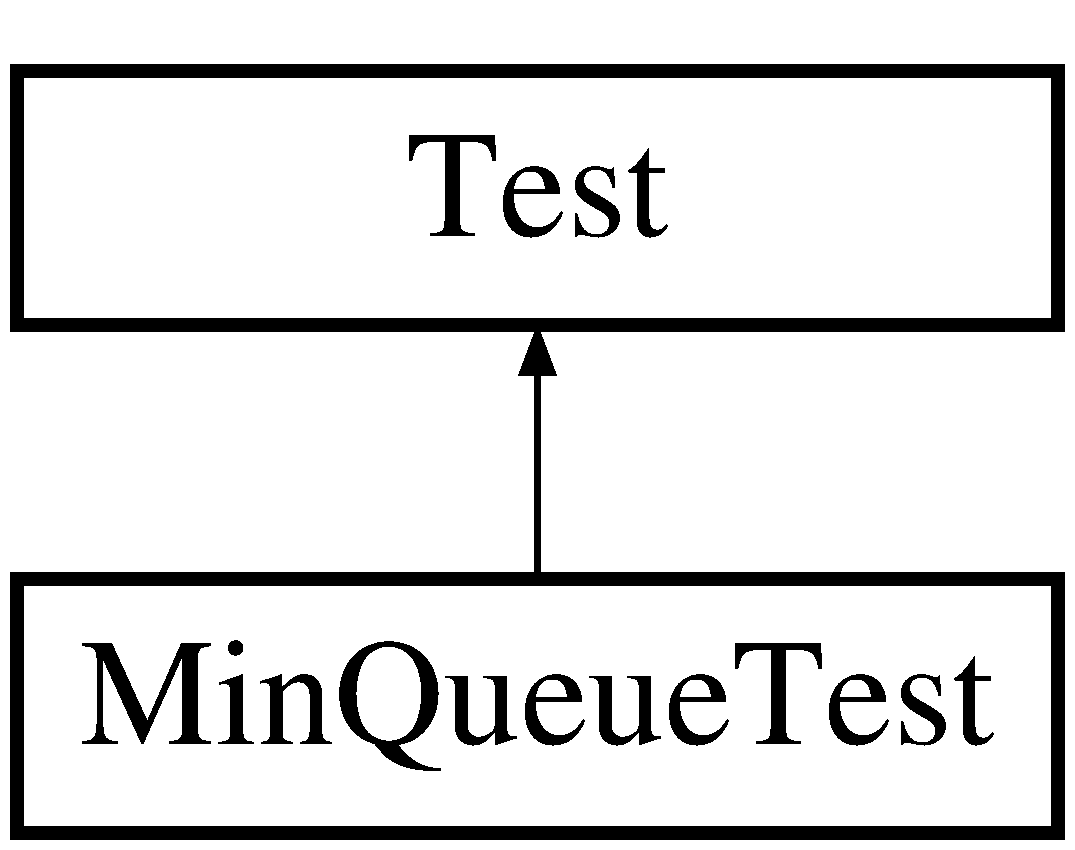
\includegraphics[height=2.000000cm]{class_min_queue_test}
\end{center}
\end{figure}
\subsection*{Public Types}
\begin{DoxyCompactItemize}
\item 
typedef std\+::function$<$ bool(std\+::shared\+\_\+ptr$<$ int $>$, std\+::shared\+\_\+ptr$<$ int $>$)$>$ \hyperlink{class_min_queue_test_a627ceae9e25205d70955137bbfc863fd}{Int\+\_\+\+Compare\+\_\+\+Type}
\item 
typedef std\+::function$<$ int \&(std\+::shared\+\_\+ptr$<$ int $>$)$>$ \hyperlink{class_min_queue_test_a40648c6c5c338387bda62519dc99fc79}{Int\+\_\+\+Get\+\_\+\+Type}
\item 
typedef std\+::function$<$ bool(std\+::shared\+\_\+ptr$<$ \hyperlink{struct_node}{Node} $>$, std\+::shared\+\_\+ptr$<$ \hyperlink{struct_node}{Node} $>$)$>$ \hyperlink{class_min_queue_test_a25bfd5b74968c587db57133f107a5f61}{Struct\+\_\+\+Compare\+\_\+\+Type}
\item 
typedef std\+::function$<$ double \&(std\+::shared\+\_\+ptr$<$ \hyperlink{struct_node}{Node} $>$)$>$ \hyperlink{class_min_queue_test_aebcf6172ed7e9dd6f821fb1043f1cd6f}{Struct\+\_\+\+Get\+\_\+\+Type}
\item 
typedef \hyperlink{class_introduction_to_algorithm_1_1_queue_algorithm_1_1_min_queue}{Min\+Queue}$<$ \hyperlink{struct_node}{Node}, double $>$ \hyperlink{class_min_queue_test_a9b7e5e987d5e856adc5beb6986dd96a3}{Struct\+\_\+\+Min\+Queue\+\_\+\+Type}
\item 
typedef \hyperlink{class_introduction_to_algorithm_1_1_queue_algorithm_1_1_min_queue}{Min\+Queue}$<$ int, int $>$ \hyperlink{class_min_queue_test_ad81df38acc845934accb320c4dbdd582}{Int\+\_\+\+Min\+Queue\+\_\+\+Type}
\end{DoxyCompactItemize}
\subsection*{Protected Member Functions}
\begin{DoxyCompactItemize}
\item 
void \hyperlink{class_min_queue_test_ae801d45bf78b7bb80b278264d3a8e96a}{Set\+Up} ()
\item 
void \hyperlink{class_min_queue_test_a3e949d54ecada54f713ff47d80eb513c}{Tear\+Down} ()
\end{DoxyCompactItemize}
\subsection*{Protected Attributes}
\begin{DoxyCompactItemize}
\item 
std\+::shared\+\_\+ptr$<$ \hyperlink{class_min_queue_test_a9b7e5e987d5e856adc5beb6986dd96a3}{Struct\+\_\+\+Min\+Queue\+\_\+\+Type} $>$ \hyperlink{class_min_queue_test_aed079eb9c6dd8460cc785b0fc6088a97}{\+\_\+strcut\+\_\+minqueue}
\item 
std\+::shared\+\_\+ptr$<$ \hyperlink{class_min_queue_test_ad81df38acc845934accb320c4dbdd582}{Int\+\_\+\+Min\+Queue\+\_\+\+Type} $>$ \hyperlink{class_min_queue_test_a03f9ea0fcc4b820a539d32d6539c2df9}{\+\_\+int\+\_\+minqueue}
\end{DoxyCompactItemize}


\subsection{Detailed Description}
\hyperlink{class_min_queue_test}{Min\+Queue\+Test}\+:测试类,用于为测试提供基础数据 

{\ttfamily \hyperlink{class_min_queue_test}{Min\+Queue\+Test}}是 {\ttfamily \+::testing\+::\+Test} 的子类。它主要用于为每一个{\ttfamily T\+E\+S\+T\+\_\+\+F}准备测试环境 

Definition at line 42 of file minqueue\+\_\+test.\+h.



\subsection{Member Typedef Documentation}
\hypertarget{class_min_queue_test_a627ceae9e25205d70955137bbfc863fd}{}\index{Min\+Queue\+Test@{Min\+Queue\+Test}!Int\+\_\+\+Compare\+\_\+\+Type@{Int\+\_\+\+Compare\+\_\+\+Type}}
\index{Int\+\_\+\+Compare\+\_\+\+Type@{Int\+\_\+\+Compare\+\_\+\+Type}!Min\+Queue\+Test@{Min\+Queue\+Test}}
\subsubsection[{Int\+\_\+\+Compare\+\_\+\+Type}]{\setlength{\rightskip}{0pt plus 5cm}typedef std\+::function$<$bool (std\+::shared\+\_\+ptr$<$int$>$,std\+::shared\+\_\+ptr$<$int$>$)$>$ {\bf Min\+Queue\+Test\+::\+Int\+\_\+\+Compare\+\_\+\+Type}}\label{class_min_queue_test_a627ceae9e25205d70955137bbfc863fd}
当最小优先级队列存放的是int$\ast$数据时,相应的比较函数对象 

Definition at line 45 of file minqueue\+\_\+test.\+h.

\hypertarget{class_min_queue_test_a40648c6c5c338387bda62519dc99fc79}{}\index{Min\+Queue\+Test@{Min\+Queue\+Test}!Int\+\_\+\+Get\+\_\+\+Type@{Int\+\_\+\+Get\+\_\+\+Type}}
\index{Int\+\_\+\+Get\+\_\+\+Type@{Int\+\_\+\+Get\+\_\+\+Type}!Min\+Queue\+Test@{Min\+Queue\+Test}}
\subsubsection[{Int\+\_\+\+Get\+\_\+\+Type}]{\setlength{\rightskip}{0pt plus 5cm}typedef std\+::function$<$int\&(std\+::shared\+\_\+ptr$<$int$>$)$>$ {\bf Min\+Queue\+Test\+::\+Int\+\_\+\+Get\+\_\+\+Type}}\label{class_min_queue_test_a40648c6c5c338387bda62519dc99fc79}
当最小优先级队列存放的是int$\ast$数据时,获取key的函数对象 

Definition at line 46 of file minqueue\+\_\+test.\+h.

\hypertarget{class_min_queue_test_ad81df38acc845934accb320c4dbdd582}{}\index{Min\+Queue\+Test@{Min\+Queue\+Test}!Int\+\_\+\+Min\+Queue\+\_\+\+Type@{Int\+\_\+\+Min\+Queue\+\_\+\+Type}}
\index{Int\+\_\+\+Min\+Queue\+\_\+\+Type@{Int\+\_\+\+Min\+Queue\+\_\+\+Type}!Min\+Queue\+Test@{Min\+Queue\+Test}}
\subsubsection[{Int\+\_\+\+Min\+Queue\+\_\+\+Type}]{\setlength{\rightskip}{0pt plus 5cm}typedef {\bf Min\+Queue}$<$int,int$>$ {\bf Min\+Queue\+Test\+::\+Int\+\_\+\+Min\+Queue\+\_\+\+Type}}\label{class_min_queue_test_ad81df38acc845934accb320c4dbdd582}
存放的是\+Node$\ast$数据的最小优先级队列,\+Node的关键字是double类型 

Definition at line 50 of file minqueue\+\_\+test.\+h.

\hypertarget{class_min_queue_test_a25bfd5b74968c587db57133f107a5f61}{}\index{Min\+Queue\+Test@{Min\+Queue\+Test}!Struct\+\_\+\+Compare\+\_\+\+Type@{Struct\+\_\+\+Compare\+\_\+\+Type}}
\index{Struct\+\_\+\+Compare\+\_\+\+Type@{Struct\+\_\+\+Compare\+\_\+\+Type}!Min\+Queue\+Test@{Min\+Queue\+Test}}
\subsubsection[{Struct\+\_\+\+Compare\+\_\+\+Type}]{\setlength{\rightskip}{0pt plus 5cm}typedef std\+::function$<$bool (std\+::shared\+\_\+ptr$<${\bf Node}$>$,std\+::shared\+\_\+ptr$<${\bf Node}$>$)$>$ {\bf Min\+Queue\+Test\+::\+Struct\+\_\+\+Compare\+\_\+\+Type}}\label{class_min_queue_test_a25bfd5b74968c587db57133f107a5f61}
当最小优先级队列存放的是\+Node$\ast$数据时,相应的比较函数对象 

Definition at line 47 of file minqueue\+\_\+test.\+h.

\hypertarget{class_min_queue_test_aebcf6172ed7e9dd6f821fb1043f1cd6f}{}\index{Min\+Queue\+Test@{Min\+Queue\+Test}!Struct\+\_\+\+Get\+\_\+\+Type@{Struct\+\_\+\+Get\+\_\+\+Type}}
\index{Struct\+\_\+\+Get\+\_\+\+Type@{Struct\+\_\+\+Get\+\_\+\+Type}!Min\+Queue\+Test@{Min\+Queue\+Test}}
\subsubsection[{Struct\+\_\+\+Get\+\_\+\+Type}]{\setlength{\rightskip}{0pt plus 5cm}typedef std\+::function$<$double\&(std\+::shared\+\_\+ptr$<${\bf Node}$>$)$>$ {\bf Min\+Queue\+Test\+::\+Struct\+\_\+\+Get\+\_\+\+Type}}\label{class_min_queue_test_aebcf6172ed7e9dd6f821fb1043f1cd6f}
当最小优先级队列存放的是\+Node$\ast$数据时,获取key的函数对象 

Definition at line 48 of file minqueue\+\_\+test.\+h.

\hypertarget{class_min_queue_test_a9b7e5e987d5e856adc5beb6986dd96a3}{}\index{Min\+Queue\+Test@{Min\+Queue\+Test}!Struct\+\_\+\+Min\+Queue\+\_\+\+Type@{Struct\+\_\+\+Min\+Queue\+\_\+\+Type}}
\index{Struct\+\_\+\+Min\+Queue\+\_\+\+Type@{Struct\+\_\+\+Min\+Queue\+\_\+\+Type}!Min\+Queue\+Test@{Min\+Queue\+Test}}
\subsubsection[{Struct\+\_\+\+Min\+Queue\+\_\+\+Type}]{\setlength{\rightskip}{0pt plus 5cm}typedef {\bf Min\+Queue}$<${\bf Node},double$>$ {\bf Min\+Queue\+Test\+::\+Struct\+\_\+\+Min\+Queue\+\_\+\+Type}}\label{class_min_queue_test_a9b7e5e987d5e856adc5beb6986dd96a3}
存放的是int$\ast$数据的最小优先级队列,其关键字就是int本身 

Definition at line 49 of file minqueue\+\_\+test.\+h.



\subsection{Member Function Documentation}
\hypertarget{class_min_queue_test_ae801d45bf78b7bb80b278264d3a8e96a}{}\index{Min\+Queue\+Test@{Min\+Queue\+Test}!Set\+Up@{Set\+Up}}
\index{Set\+Up@{Set\+Up}!Min\+Queue\+Test@{Min\+Queue\+Test}}
\subsubsection[{Set\+Up()}]{\setlength{\rightskip}{0pt plus 5cm}void Min\+Queue\+Test\+::\+Set\+Up (
\begin{DoxyParamCaption}
{}
\end{DoxyParamCaption}
)\hspace{0.3cm}{\ttfamily [inline]}, {\ttfamily [protected]}}\label{class_min_queue_test_ae801d45bf78b7bb80b278264d3a8e96a}


Definition at line 52 of file minqueue\+\_\+test.\+h.

\hypertarget{class_min_queue_test_a3e949d54ecada54f713ff47d80eb513c}{}\index{Min\+Queue\+Test@{Min\+Queue\+Test}!Tear\+Down@{Tear\+Down}}
\index{Tear\+Down@{Tear\+Down}!Min\+Queue\+Test@{Min\+Queue\+Test}}
\subsubsection[{Tear\+Down()}]{\setlength{\rightskip}{0pt plus 5cm}void Min\+Queue\+Test\+::\+Tear\+Down (
\begin{DoxyParamCaption}
{}
\end{DoxyParamCaption}
)\hspace{0.3cm}{\ttfamily [inline]}, {\ttfamily [protected]}}\label{class_min_queue_test_a3e949d54ecada54f713ff47d80eb513c}


Definition at line 62 of file minqueue\+\_\+test.\+h.



\subsection{Member Data Documentation}
\hypertarget{class_min_queue_test_a03f9ea0fcc4b820a539d32d6539c2df9}{}\index{Min\+Queue\+Test@{Min\+Queue\+Test}!\+\_\+int\+\_\+minqueue@{\+\_\+int\+\_\+minqueue}}
\index{\+\_\+int\+\_\+minqueue@{\+\_\+int\+\_\+minqueue}!Min\+Queue\+Test@{Min\+Queue\+Test}}
\subsubsection[{\+\_\+int\+\_\+minqueue}]{\setlength{\rightskip}{0pt plus 5cm}std\+::shared\+\_\+ptr$<${\bf Int\+\_\+\+Min\+Queue\+\_\+\+Type}$>$ Min\+Queue\+Test\+::\+\_\+int\+\_\+minqueue\hspace{0.3cm}{\ttfamily [protected]}}\label{class_min_queue_test_a03f9ea0fcc4b820a539d32d6539c2df9}
指向一个最小优先级队列 

Definition at line 64 of file minqueue\+\_\+test.\+h.

\hypertarget{class_min_queue_test_aed079eb9c6dd8460cc785b0fc6088a97}{}\index{Min\+Queue\+Test@{Min\+Queue\+Test}!\+\_\+strcut\+\_\+minqueue@{\+\_\+strcut\+\_\+minqueue}}
\index{\+\_\+strcut\+\_\+minqueue@{\+\_\+strcut\+\_\+minqueue}!Min\+Queue\+Test@{Min\+Queue\+Test}}
\subsubsection[{\+\_\+strcut\+\_\+minqueue}]{\setlength{\rightskip}{0pt plus 5cm}std\+::shared\+\_\+ptr$<${\bf Struct\+\_\+\+Min\+Queue\+\_\+\+Type}$>$ Min\+Queue\+Test\+::\+\_\+strcut\+\_\+minqueue\hspace{0.3cm}{\ttfamily [protected]}}\label{class_min_queue_test_aed079eb9c6dd8460cc785b0fc6088a97}
指向一个最小优先级队列 

Definition at line 63 of file minqueue\+\_\+test.\+h.



The documentation for this class was generated from the following file\+:\begin{DoxyCompactItemize}
\item 
src/queue\+\_\+algorithms/min\+\_\+queue/\hyperlink{minqueue__test_8h}{minqueue\+\_\+test.\+h}\end{DoxyCompactItemize}

\hypertarget{struct_node}{}\section{Node Struct Reference}
\label{struct_node}\index{Node@{Node}}


\hyperlink{struct_node}{Node}\+:用于测试的类型  




{\ttfamily \#include $<$minqueue\+\_\+test.\+h$>$}

\subsection*{Public Member Functions}
\begin{DoxyCompactItemize}
\item 
\hyperlink{struct_node_a3c69606b98be4c0fe6cc2abbe554948e}{Node} (int k)
\end{DoxyCompactItemize}
\subsection*{Public Attributes}
\begin{DoxyCompactItemize}
\item 
double \hyperlink{struct_node_afcabbedc2b739455060451607c6344e4}{key}
\end{DoxyCompactItemize}


\subsection{Detailed Description}
\hyperlink{struct_node}{Node}\+:用于测试的类型 

Definition at line 31 of file minqueue\+\_\+test.\+h.



\subsection{Constructor \& Destructor Documentation}
\hypertarget{struct_node_a3c69606b98be4c0fe6cc2abbe554948e}{}\index{Node@{Node}!Node@{Node}}
\index{Node@{Node}!Node@{Node}}
\subsubsection[{Node(int k)}]{\setlength{\rightskip}{0pt plus 5cm}Node\+::\+Node (
\begin{DoxyParamCaption}
\item[{int}]{k}
\end{DoxyParamCaption}
)\hspace{0.3cm}{\ttfamily [inline]}}\label{struct_node_a3c69606b98be4c0fe6cc2abbe554948e}


Definition at line 33 of file minqueue\+\_\+test.\+h.



\subsection{Member Data Documentation}
\hypertarget{struct_node_afcabbedc2b739455060451607c6344e4}{}\index{Node@{Node}!key@{key}}
\index{key@{key}!Node@{Node}}
\subsubsection[{key}]{\setlength{\rightskip}{0pt plus 5cm}double Node\+::key}\label{struct_node_afcabbedc2b739455060451607c6344e4}
key存放数据 

Definition at line 34 of file minqueue\+\_\+test.\+h.



The documentation for this struct was generated from the following file\+:\begin{DoxyCompactItemize}
\item 
src/queue\+\_\+algorithms/min\+\_\+queue/\hyperlink{minqueue__test_8h}{minqueue\+\_\+test.\+h}\end{DoxyCompactItemize}

\hypertarget{class_prim_test}{}\section{Prim\+Test Class Reference}
\label{class_prim_test}\index{Prim\+Test@{Prim\+Test}}


\hyperlink{class_prim_test}{Prim\+Test}\+:测试类,用于为测试提供基础数据  




{\ttfamily \#include $<$prim\+\_\+test.\+h$>$}

Inheritance diagram for Prim\+Test\+:\begin{figure}[H]
\begin{center}
\leavevmode
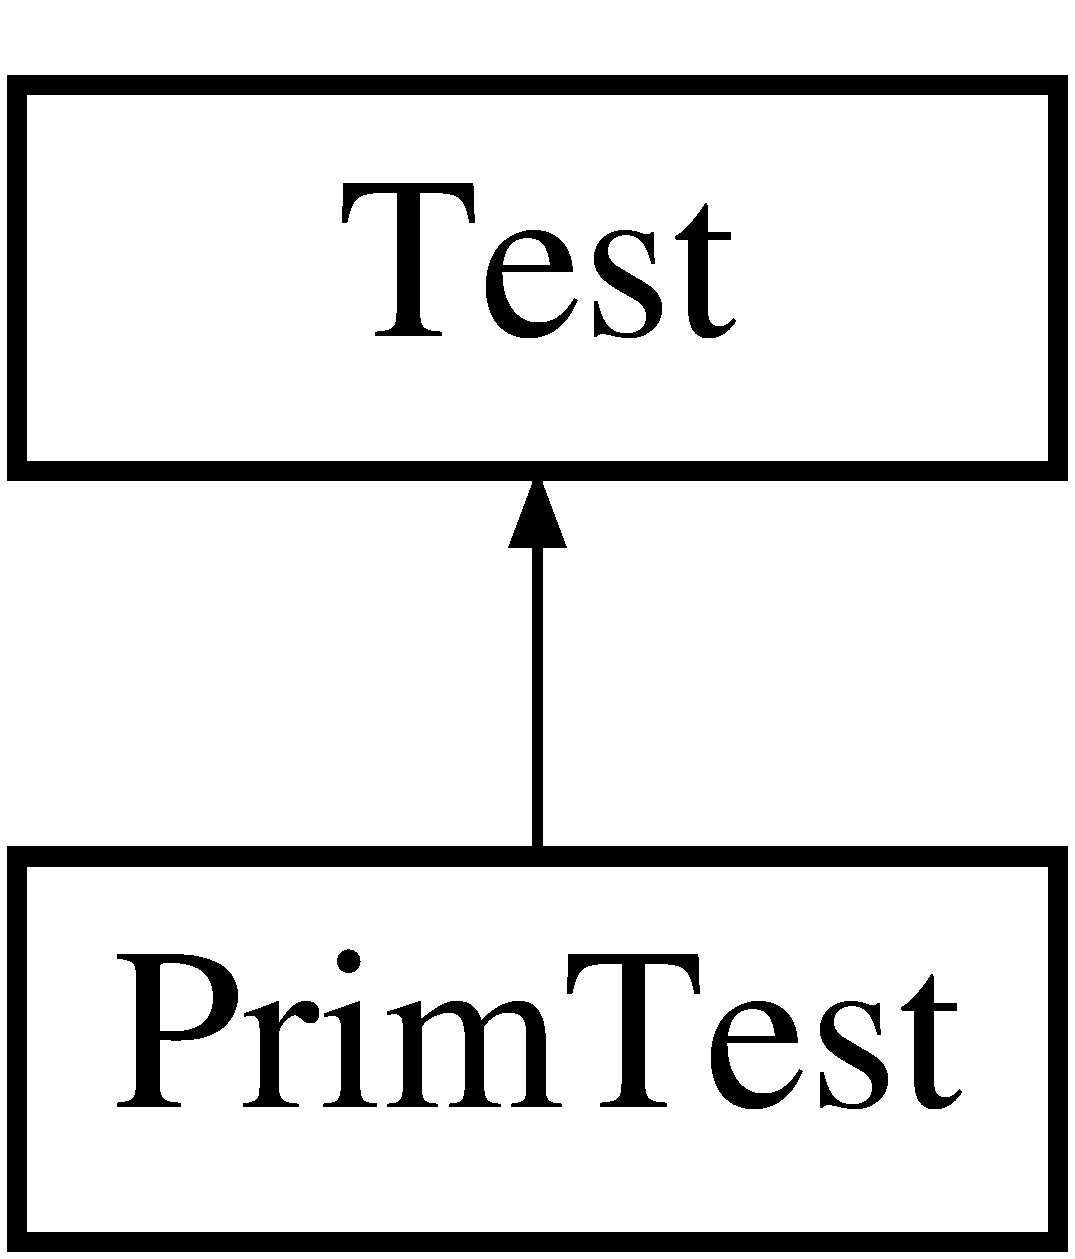
\includegraphics[height=2.000000cm]{class_prim_test}
\end{center}
\end{figure}
\subsection*{Public Types}
\begin{DoxyCompactItemize}
\item 
typedef \hyperlink{struct_introduction_to_algorithm_1_1_graph_algorithm_1_1_graph}{Graph}$<$ P\+R\+I\+M\+\_\+\+N, \hyperlink{struct_introduction_to_algorithm_1_1_graph_algorithm_1_1_vertex_p}{Vertex\+P}$<$ int $>$ $>$ \hyperlink{class_prim_test_a007bd8e1bdac3f8548d0a4bebce87881}{G\+Type}
\item 
typedef std\+::function$<$ void(\hyperlink{struct_introduction_to_algorithm_1_1_graph_algorithm_1_1_vertex_p}{Vertex\+P}$<$ int $>$\+::V\+I\+D\+Type v\+\_\+id)$>$ \hyperlink{class_prim_test_a834237db99fdb38480aa6ba46b509e9e}{Action\+Type}
\end{DoxyCompactItemize}
\subsection*{Protected Member Functions}
\begin{DoxyCompactItemize}
\item 
void \hyperlink{class_prim_test_a9f2e77a9785f9ae04e8c3ea72fb6b127}{Set\+Up} ()
\item 
void \hyperlink{class_prim_test_a5894c9275a0bfda59f7b5661ece6b984}{Tear\+Down} ()
\end{DoxyCompactItemize}
\subsection*{Protected Attributes}
\begin{DoxyCompactItemize}
\item 
std\+::shared\+\_\+ptr$<$ \hyperlink{class_prim_test_a007bd8e1bdac3f8548d0a4bebce87881}{G\+Type} $>$ \hyperlink{class_prim_test_a7ff7449d84167db478a33a4dbb1b2e78}{\+\_\+1v\+\_\+graph}
\item 
std\+::shared\+\_\+ptr$<$ \hyperlink{class_prim_test_a007bd8e1bdac3f8548d0a4bebce87881}{G\+Type} $>$ \hyperlink{class_prim_test_a256859b15df61e1cd0c96065bf19dc71}{\+\_\+1e\+\_\+graph}
\item 
std\+::shared\+\_\+ptr$<$ \hyperlink{class_prim_test_a007bd8e1bdac3f8548d0a4bebce87881}{G\+Type} $>$ \hyperlink{class_prim_test_aeac490b81dfcef56b2a8b656942b012a}{\+\_\+list\+\_\+graph}
\item 
std\+::shared\+\_\+ptr$<$ \hyperlink{class_prim_test_a007bd8e1bdac3f8548d0a4bebce87881}{G\+Type} $>$ \hyperlink{class_prim_test_a25281c926fc389770548b0f035e41615}{\+\_\+all\+\_\+edges\+\_\+graph}
\end{DoxyCompactItemize}


\subsection{Detailed Description}
\hyperlink{class_prim_test}{Prim\+Test}\+:测试类,用于为测试提供基础数据 

{\ttfamily \hyperlink{class_prim_test}{Prim\+Test}}是 {\ttfamily \+::testing\+::\+Test} 的子类。它主要用于为每一个{\ttfamily T\+E\+S\+T\+\_\+\+F}准备测试环境 

Definition at line 38 of file prim\+\_\+test.\+h.



\subsection{Member Typedef Documentation}
\hypertarget{class_prim_test_a834237db99fdb38480aa6ba46b509e9e}{}\index{Prim\+Test@{Prim\+Test}!Action\+Type@{Action\+Type}}
\index{Action\+Type@{Action\+Type}!Prim\+Test@{Prim\+Test}}
\subsubsection[{Action\+Type}]{\setlength{\rightskip}{0pt plus 5cm}typedef std\+::function$<$void({\bf Vertex\+P}$<$int$>$\+::V\+I\+D\+Type v\+\_\+id)$>$ {\bf Prim\+Test\+::\+Action\+Type}}\label{class_prim_test_a834237db99fdb38480aa6ba46b509e9e}
模板实例化的\+Action类型 

Definition at line 42 of file prim\+\_\+test.\+h.

\hypertarget{class_prim_test_a007bd8e1bdac3f8548d0a4bebce87881}{}\index{Prim\+Test@{Prim\+Test}!G\+Type@{G\+Type}}
\index{G\+Type@{G\+Type}!Prim\+Test@{Prim\+Test}}
\subsubsection[{G\+Type}]{\setlength{\rightskip}{0pt plus 5cm}typedef {\bf Graph}$<$P\+R\+I\+M\+\_\+\+N,{\bf Vertex\+P}$<$int$>$ $>$ {\bf Prim\+Test\+::\+G\+Type}}\label{class_prim_test_a007bd8e1bdac3f8548d0a4bebce87881}
模板实例化的图类型,该图的顶点类型为{\ttfamily Vertex\+P$<$int$>$} 

Definition at line 41 of file prim\+\_\+test.\+h.



\subsection{Member Function Documentation}
\hypertarget{class_prim_test_a9f2e77a9785f9ae04e8c3ea72fb6b127}{}\index{Prim\+Test@{Prim\+Test}!Set\+Up@{Set\+Up}}
\index{Set\+Up@{Set\+Up}!Prim\+Test@{Prim\+Test}}
\subsubsection[{Set\+Up()}]{\setlength{\rightskip}{0pt plus 5cm}void Prim\+Test\+::\+Set\+Up (
\begin{DoxyParamCaption}
{}
\end{DoxyParamCaption}
)\hspace{0.3cm}{\ttfamily [inline]}, {\ttfamily [protected]}}\label{class_prim_test_a9f2e77a9785f9ae04e8c3ea72fb6b127}


Definition at line 44 of file prim\+\_\+test.\+h.

\hypertarget{class_prim_test_a5894c9275a0bfda59f7b5661ece6b984}{}\index{Prim\+Test@{Prim\+Test}!Tear\+Down@{Tear\+Down}}
\index{Tear\+Down@{Tear\+Down}!Prim\+Test@{Prim\+Test}}
\subsubsection[{Tear\+Down()}]{\setlength{\rightskip}{0pt plus 5cm}void Prim\+Test\+::\+Tear\+Down (
\begin{DoxyParamCaption}
{}
\end{DoxyParamCaption}
)\hspace{0.3cm}{\ttfamily [inline]}, {\ttfamily [protected]}}\label{class_prim_test_a5894c9275a0bfda59f7b5661ece6b984}


Definition at line 71 of file prim\+\_\+test.\+h.



\subsection{Member Data Documentation}
\hypertarget{class_prim_test_a256859b15df61e1cd0c96065bf19dc71}{}\index{Prim\+Test@{Prim\+Test}!\+\_\+1e\+\_\+graph@{\+\_\+1e\+\_\+graph}}
\index{\+\_\+1e\+\_\+graph@{\+\_\+1e\+\_\+graph}!Prim\+Test@{Prim\+Test}}
\subsubsection[{\+\_\+1e\+\_\+graph}]{\setlength{\rightskip}{0pt plus 5cm}std\+::shared\+\_\+ptr$<${\bf G\+Type}$>$ Prim\+Test\+::\+\_\+1e\+\_\+graph\hspace{0.3cm}{\ttfamily [protected]}}\label{class_prim_test_a256859b15df61e1cd0c96065bf19dc71}
指向一个图,该图只有一条边 

Definition at line 73 of file prim\+\_\+test.\+h.

\hypertarget{class_prim_test_a7ff7449d84167db478a33a4dbb1b2e78}{}\index{Prim\+Test@{Prim\+Test}!\+\_\+1v\+\_\+graph@{\+\_\+1v\+\_\+graph}}
\index{\+\_\+1v\+\_\+graph@{\+\_\+1v\+\_\+graph}!Prim\+Test@{Prim\+Test}}
\subsubsection[{\+\_\+1v\+\_\+graph}]{\setlength{\rightskip}{0pt plus 5cm}std\+::shared\+\_\+ptr$<${\bf G\+Type}$>$ Prim\+Test\+::\+\_\+1v\+\_\+graph\hspace{0.3cm}{\ttfamily [protected]}}\label{class_prim_test_a7ff7449d84167db478a33a4dbb1b2e78}
指向一个图,该图只有一个顶点 

Definition at line 72 of file prim\+\_\+test.\+h.

\hypertarget{class_prim_test_a25281c926fc389770548b0f035e41615}{}\index{Prim\+Test@{Prim\+Test}!\+\_\+all\+\_\+edges\+\_\+graph@{\+\_\+all\+\_\+edges\+\_\+graph}}
\index{\+\_\+all\+\_\+edges\+\_\+graph@{\+\_\+all\+\_\+edges\+\_\+graph}!Prim\+Test@{Prim\+Test}}
\subsubsection[{\+\_\+all\+\_\+edges\+\_\+graph}]{\setlength{\rightskip}{0pt plus 5cm}std\+::shared\+\_\+ptr$<${\bf G\+Type}$>$ Prim\+Test\+::\+\_\+all\+\_\+edges\+\_\+graph\hspace{0.3cm}{\ttfamily [protected]}}\label{class_prim_test_a25281c926fc389770548b0f035e41615}
指向一个图,该图中任意一对顶点之间都有边 

Definition at line 75 of file prim\+\_\+test.\+h.

\hypertarget{class_prim_test_aeac490b81dfcef56b2a8b656942b012a}{}\index{Prim\+Test@{Prim\+Test}!\+\_\+list\+\_\+graph@{\+\_\+list\+\_\+graph}}
\index{\+\_\+list\+\_\+graph@{\+\_\+list\+\_\+graph}!Prim\+Test@{Prim\+Test}}
\subsubsection[{\+\_\+list\+\_\+graph}]{\setlength{\rightskip}{0pt plus 5cm}std\+::shared\+\_\+ptr$<${\bf G\+Type}$>$ Prim\+Test\+::\+\_\+list\+\_\+graph\hspace{0.3cm}{\ttfamily [protected]}}\label{class_prim_test_aeac490b81dfcef56b2a8b656942b012a}
指向一个图,该图的边组成一个链条 

Definition at line 74 of file prim\+\_\+test.\+h.



The documentation for this class was generated from the following file\+:\begin{DoxyCompactItemize}
\item 
src/graph\+\_\+algorithms/minimum\+\_\+spanning\+\_\+tree/prim/\hyperlink{prim__test_8h}{prim\+\_\+test.\+h}\end{DoxyCompactItemize}

\hypertarget{class_relabel_to_front_test}{}\section{Relabel\+To\+Front\+Test Class Reference}
\label{class_relabel_to_front_test}\index{Relabel\+To\+Front\+Test@{Relabel\+To\+Front\+Test}}


\hyperlink{class_relabel_to_front_test}{Relabel\+To\+Front\+Test}\+:测试类,用于为测试提供基础数据  




{\ttfamily \#include $<$relabeltofront\+\_\+test.\+h$>$}

Inheritance diagram for Relabel\+To\+Front\+Test\+:\begin{figure}[H]
\begin{center}
\leavevmode
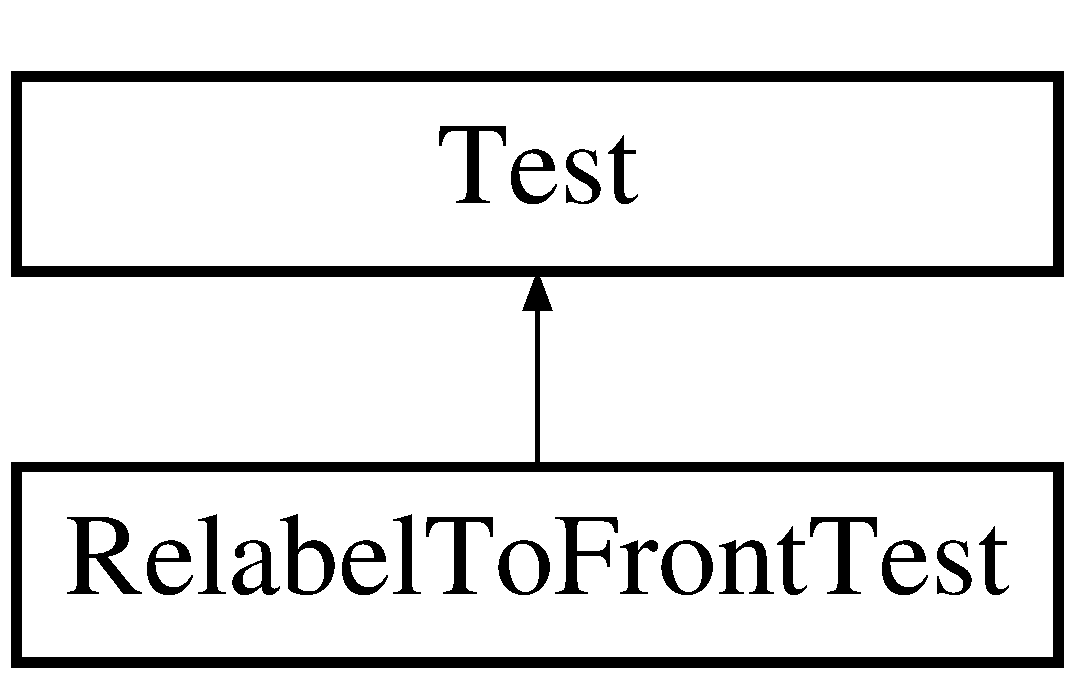
\includegraphics[height=2.000000cm]{class_relabel_to_front_test}
\end{center}
\end{figure}
\subsection*{Public Types}
\begin{DoxyCompactItemize}
\item 
typedef \hyperlink{struct_introduction_to_algorithm_1_1_graph_algorithm_1_1_graph}{Graph}$<$ R\+T\+F\+\_\+\+N, \hyperlink{struct_introduction_to_algorithm_1_1_graph_algorithm_1_1_front_flow_vertex}{Front\+Flow\+Vertex}$<$ int $>$ $>$ \hyperlink{class_relabel_to_front_test_a50ca1a0a59136fe999254bdfb2b21a7b}{G\+Type}
\end{DoxyCompactItemize}
\subsection*{Protected Member Functions}
\begin{DoxyCompactItemize}
\item 
void \hyperlink{class_relabel_to_front_test_a52350917cedfacccb9fe544ce86e13e0}{Set\+Up} ()
\item 
void \hyperlink{class_relabel_to_front_test_a8ee298a2969fd037af9b263d127c1a06}{Tear\+Down} ()
\end{DoxyCompactItemize}
\subsection*{Protected Attributes}
\begin{DoxyCompactItemize}
\item 
std\+::shared\+\_\+ptr$<$ \hyperlink{class_relabel_to_front_test_a50ca1a0a59136fe999254bdfb2b21a7b}{G\+Type} $>$ \hyperlink{class_relabel_to_front_test_a3eecd133a6421543cc88cff1b7ffa6f2}{\+\_\+graph}
\end{DoxyCompactItemize}


\subsection{Detailed Description}
\hyperlink{class_relabel_to_front_test}{Relabel\+To\+Front\+Test}\+:测试类,用于为测试提供基础数据 

{\ttfamily \hyperlink{class_relabel_to_front_test}{Relabel\+To\+Front\+Test}}是 {\ttfamily \+::testing\+::\+Test} 的子类。它主要用于为每一个{\ttfamily T\+E\+S\+T\+\_\+\+F}准备测试环境 

Definition at line 38 of file relabeltofront\+\_\+test.\+h.



\subsection{Member Typedef Documentation}
\hypertarget{class_relabel_to_front_test_a50ca1a0a59136fe999254bdfb2b21a7b}{}\index{Relabel\+To\+Front\+Test@{Relabel\+To\+Front\+Test}!G\+Type@{G\+Type}}
\index{G\+Type@{G\+Type}!Relabel\+To\+Front\+Test@{Relabel\+To\+Front\+Test}}
\subsubsection[{G\+Type}]{\setlength{\rightskip}{0pt plus 5cm}typedef {\bf Graph}$<$R\+T\+F\+\_\+\+N,{\bf Front\+Flow\+Vertex}$<$int$>$ $>$ {\bf Relabel\+To\+Front\+Test\+::\+G\+Type}}\label{class_relabel_to_front_test_a50ca1a0a59136fe999254bdfb2b21a7b}
模板实例化的图类型,该图的顶点类型为{\ttfamily Front\+Flow\+Vertex$<$int$>$} 

Definition at line 41 of file relabeltofront\+\_\+test.\+h.



\subsection{Member Function Documentation}
\hypertarget{class_relabel_to_front_test_a52350917cedfacccb9fe544ce86e13e0}{}\index{Relabel\+To\+Front\+Test@{Relabel\+To\+Front\+Test}!Set\+Up@{Set\+Up}}
\index{Set\+Up@{Set\+Up}!Relabel\+To\+Front\+Test@{Relabel\+To\+Front\+Test}}
\subsubsection[{Set\+Up()}]{\setlength{\rightskip}{0pt plus 5cm}void Relabel\+To\+Front\+Test\+::\+Set\+Up (
\begin{DoxyParamCaption}
{}
\end{DoxyParamCaption}
)\hspace{0.3cm}{\ttfamily [inline]}, {\ttfamily [protected]}}\label{class_relabel_to_front_test_a52350917cedfacccb9fe544ce86e13e0}


Definition at line 44 of file relabeltofront\+\_\+test.\+h.

\hypertarget{class_relabel_to_front_test_a8ee298a2969fd037af9b263d127c1a06}{}\index{Relabel\+To\+Front\+Test@{Relabel\+To\+Front\+Test}!Tear\+Down@{Tear\+Down}}
\index{Tear\+Down@{Tear\+Down}!Relabel\+To\+Front\+Test@{Relabel\+To\+Front\+Test}}
\subsubsection[{Tear\+Down()}]{\setlength{\rightskip}{0pt plus 5cm}void Relabel\+To\+Front\+Test\+::\+Tear\+Down (
\begin{DoxyParamCaption}
{}
\end{DoxyParamCaption}
)\hspace{0.3cm}{\ttfamily [inline]}, {\ttfamily [protected]}}\label{class_relabel_to_front_test_a8ee298a2969fd037af9b263d127c1a06}


Definition at line 62 of file relabeltofront\+\_\+test.\+h.



\subsection{Member Data Documentation}
\hypertarget{class_relabel_to_front_test_a3eecd133a6421543cc88cff1b7ffa6f2}{}\index{Relabel\+To\+Front\+Test@{Relabel\+To\+Front\+Test}!\+\_\+graph@{\+\_\+graph}}
\index{\+\_\+graph@{\+\_\+graph}!Relabel\+To\+Front\+Test@{Relabel\+To\+Front\+Test}}
\subsubsection[{\+\_\+graph}]{\setlength{\rightskip}{0pt plus 5cm}std\+::shared\+\_\+ptr$<${\bf G\+Type}$>$ Relabel\+To\+Front\+Test\+::\+\_\+graph\hspace{0.3cm}{\ttfamily [protected]}}\label{class_relabel_to_front_test_a3eecd133a6421543cc88cff1b7ffa6f2}
指向一个图,算法导论图26-\/6 

Definition at line 63 of file relabeltofront\+\_\+test.\+h.



The documentation for this class was generated from the following file\+:\begin{DoxyCompactItemize}
\item 
src/graph\+\_\+algorithms/max\+\_\+flow/relabel\+\_\+to\+\_\+front/\hyperlink{relabeltofront__test_8h}{relabeltofront\+\_\+test.\+h}\end{DoxyCompactItemize}

\hypertarget{class_s_c_c_test}{}\section{S\+C\+C\+Test Class Reference}
\label{class_s_c_c_test}\index{S\+C\+C\+Test@{S\+C\+C\+Test}}


\hyperlink{class_s_c_c_test}{S\+C\+C\+Test}\+:测试类,用于为测试提供基础数据  




{\ttfamily \#include $<$strongconnectedcomponent\+\_\+test.\+h$>$}

Inheritance diagram for S\+C\+C\+Test\+:\begin{figure}[H]
\begin{center}
\leavevmode
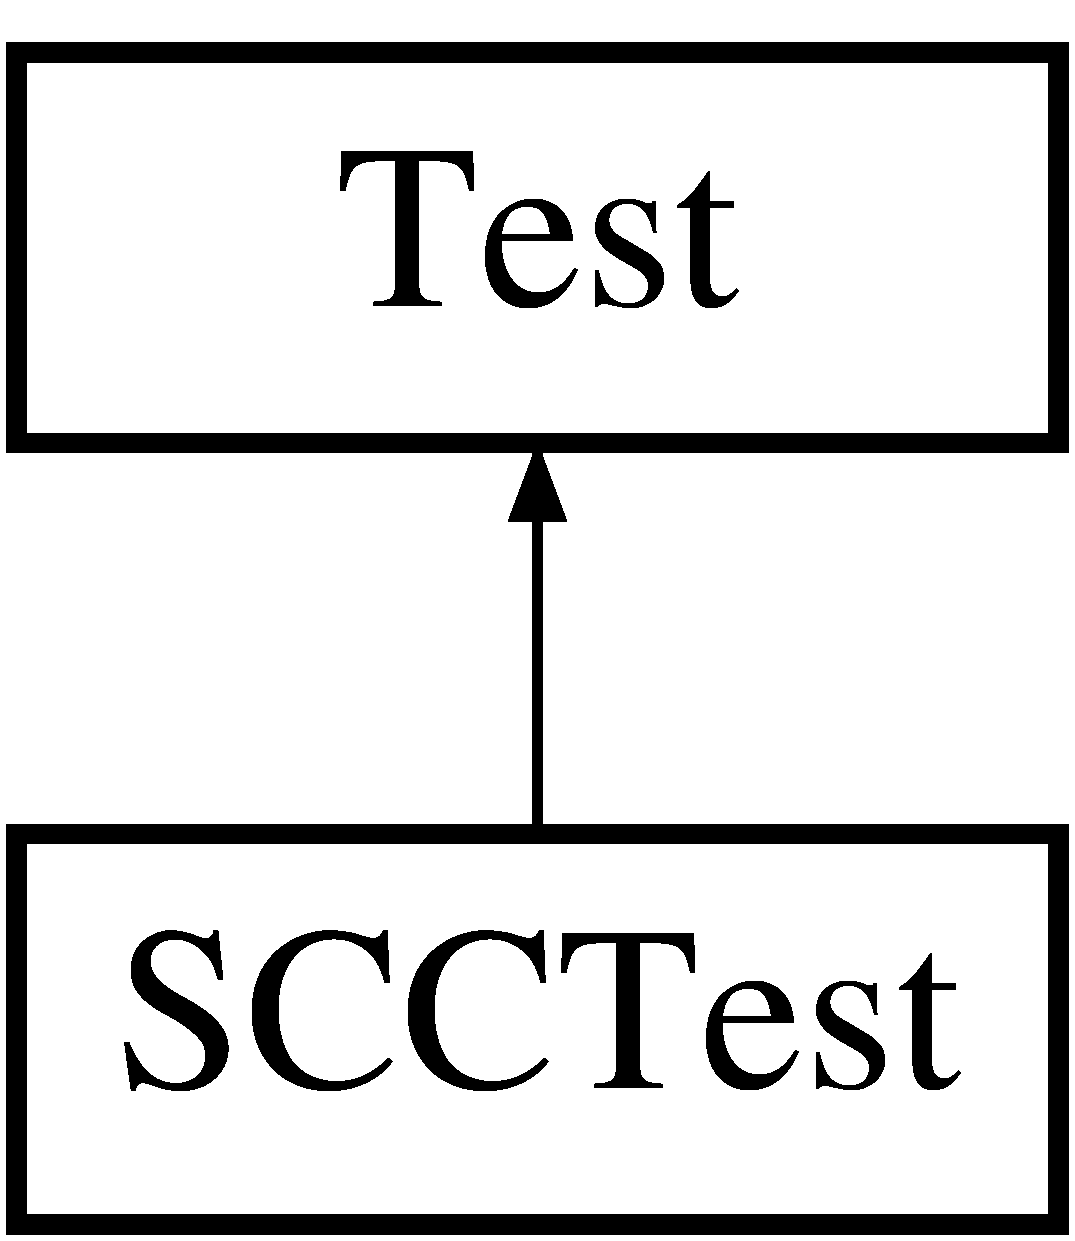
\includegraphics[height=2.000000cm]{class_s_c_c_test}
\end{center}
\end{figure}
\subsection*{Public Types}
\begin{DoxyCompactItemize}
\item 
typedef \hyperlink{struct_introduction_to_algorithm_1_1_graph_algorithm_1_1_graph}{Graph}$<$ S\+C\+C\+\_\+\+N, \hyperlink{struct_introduction_to_algorithm_1_1_graph_algorithm_1_1_d_f_s___vertex}{D\+F\+S\+\_\+\+Vertex}$<$ double $>$ $>$ \hyperlink{class_s_c_c_test_abb59a4d30b8d2bb5c08e09e902745824}{G\+Type}
\end{DoxyCompactItemize}
\subsection*{Protected Member Functions}
\begin{DoxyCompactItemize}
\item 
void \hyperlink{class_s_c_c_test_a840b86482e67f9b7e483645eea64d950}{Set\+Up} ()
\item 
void \hyperlink{class_s_c_c_test_a9de4301f4841fd61853a61399f6f9bfc}{Tear\+Down} ()
\end{DoxyCompactItemize}
\subsection*{Protected Attributes}
\begin{DoxyCompactItemize}
\item 
std\+::shared\+\_\+ptr$<$ \hyperlink{class_s_c_c_test_abb59a4d30b8d2bb5c08e09e902745824}{G\+Type} $>$ \hyperlink{class_s_c_c_test_a45ded9e0483b0f9c25bbbe8b058c8b77}{\+\_\+list\+\_\+graph}
\item 
std\+::shared\+\_\+ptr$<$ \hyperlink{class_s_c_c_test_abb59a4d30b8d2bb5c08e09e902745824}{G\+Type} $>$ \hyperlink{class_s_c_c_test_a4752a3091b185c9f5e5beddb842211e5}{\+\_\+scc\+\_\+graph}
\end{DoxyCompactItemize}


\subsection{Detailed Description}
\hyperlink{class_s_c_c_test}{S\+C\+C\+Test}\+:测试类,用于为测试提供基础数据 

{\ttfamily \hyperlink{class_s_c_c_test}{S\+C\+C\+Test}}是 {\ttfamily \+::testing\+::\+Test} 的子类。它主要用于为每一个{\ttfamily T\+E\+S\+T\+\_\+\+F}准备测试环境 

Definition at line 39 of file strongconnectedcomponent\+\_\+test.\+h.



\subsection{Member Typedef Documentation}
\hypertarget{class_s_c_c_test_abb59a4d30b8d2bb5c08e09e902745824}{}\index{S\+C\+C\+Test@{S\+C\+C\+Test}!G\+Type@{G\+Type}}
\index{G\+Type@{G\+Type}!S\+C\+C\+Test@{S\+C\+C\+Test}}
\subsubsection[{G\+Type}]{\setlength{\rightskip}{0pt plus 5cm}typedef {\bf Graph}$<$S\+C\+C\+\_\+\+N,{\bf D\+F\+S\+\_\+\+Vertex}$<$double$>$ $>$ {\bf S\+C\+C\+Test\+::\+G\+Type}}\label{class_s_c_c_test_abb59a4d30b8d2bb5c08e09e902745824}
模板实例化的图类型,该图的顶点类型为{\ttfamily D\+F\+S\+\_\+\+Vertex$<$double$>$} 

Definition at line 42 of file strongconnectedcomponent\+\_\+test.\+h.



\subsection{Member Function Documentation}
\hypertarget{class_s_c_c_test_a840b86482e67f9b7e483645eea64d950}{}\index{S\+C\+C\+Test@{S\+C\+C\+Test}!Set\+Up@{Set\+Up}}
\index{Set\+Up@{Set\+Up}!S\+C\+C\+Test@{S\+C\+C\+Test}}
\subsubsection[{Set\+Up()}]{\setlength{\rightskip}{0pt plus 5cm}void S\+C\+C\+Test\+::\+Set\+Up (
\begin{DoxyParamCaption}
{}
\end{DoxyParamCaption}
)\hspace{0.3cm}{\ttfamily [inline]}, {\ttfamily [protected]}}\label{class_s_c_c_test_a840b86482e67f9b7e483645eea64d950}


Definition at line 45 of file strongconnectedcomponent\+\_\+test.\+h.

\hypertarget{class_s_c_c_test_a9de4301f4841fd61853a61399f6f9bfc}{}\index{S\+C\+C\+Test@{S\+C\+C\+Test}!Tear\+Down@{Tear\+Down}}
\index{Tear\+Down@{Tear\+Down}!S\+C\+C\+Test@{S\+C\+C\+Test}}
\subsubsection[{Tear\+Down()}]{\setlength{\rightskip}{0pt plus 5cm}void S\+C\+C\+Test\+::\+Tear\+Down (
\begin{DoxyParamCaption}
{}
\end{DoxyParamCaption}
)\hspace{0.3cm}{\ttfamily [inline]}, {\ttfamily [protected]}}\label{class_s_c_c_test_a9de4301f4841fd61853a61399f6f9bfc}


Definition at line 65 of file strongconnectedcomponent\+\_\+test.\+h.



\subsection{Member Data Documentation}
\hypertarget{class_s_c_c_test_a45ded9e0483b0f9c25bbbe8b058c8b77}{}\index{S\+C\+C\+Test@{S\+C\+C\+Test}!\+\_\+list\+\_\+graph@{\+\_\+list\+\_\+graph}}
\index{\+\_\+list\+\_\+graph@{\+\_\+list\+\_\+graph}!S\+C\+C\+Test@{S\+C\+C\+Test}}
\subsubsection[{\+\_\+list\+\_\+graph}]{\setlength{\rightskip}{0pt plus 5cm}std\+::shared\+\_\+ptr$<${\bf G\+Type}$>$ S\+C\+C\+Test\+::\+\_\+list\+\_\+graph\hspace{0.3cm}{\ttfamily [protected]}}\label{class_s_c_c_test_a45ded9e0483b0f9c25bbbe8b058c8b77}
指向一个图,该图的边组成一个链条 

Definition at line 66 of file strongconnectedcomponent\+\_\+test.\+h.

\hypertarget{class_s_c_c_test_a4752a3091b185c9f5e5beddb842211e5}{}\index{S\+C\+C\+Test@{S\+C\+C\+Test}!\+\_\+scc\+\_\+graph@{\+\_\+scc\+\_\+graph}}
\index{\+\_\+scc\+\_\+graph@{\+\_\+scc\+\_\+graph}!S\+C\+C\+Test@{S\+C\+C\+Test}}
\subsubsection[{\+\_\+scc\+\_\+graph}]{\setlength{\rightskip}{0pt plus 5cm}std\+::shared\+\_\+ptr$<${\bf G\+Type}$>$ S\+C\+C\+Test\+::\+\_\+scc\+\_\+graph\hspace{0.3cm}{\ttfamily [protected]}}\label{class_s_c_c_test_a4752a3091b185c9f5e5beddb842211e5}
指向一个图,该图的边组成一个环 

Definition at line 67 of file strongconnectedcomponent\+\_\+test.\+h.



The documentation for this class was generated from the following file\+:\begin{DoxyCompactItemize}
\item 
src/graph\+\_\+algorithms/basic\+\_\+graph/strong\+\_\+connected\+\_\+component/\hyperlink{strongconnectedcomponent__test_8h}{strongconnectedcomponent\+\_\+test.\+h}\end{DoxyCompactItemize}

\hypertarget{class_introduction_to_algorithm_1_1_tree_algorithm_1_1_search_tree}{}\section{Introduction\+To\+Algorithm\+:\+:Tree\+Algorithm\+:\+:Search\+Tree$<$ Node\+Type $>$ Class Template Reference}
\label{class_introduction_to_algorithm_1_1_tree_algorithm_1_1_search_tree}\index{Introduction\+To\+Algorithm\+::\+Tree\+Algorithm\+::\+Search\+Tree$<$ Node\+Type $>$@{Introduction\+To\+Algorithm\+::\+Tree\+Algorithm\+::\+Search\+Tree$<$ Node\+Type $>$}}


Search\+Tree:二叉搜索树,算法导论12章  




{\ttfamily \#include $<$searchtree.\+h$>$}

Inheritance diagram for Introduction\+To\+Algorithm\+:\+:Tree\+Algorithm\+:\+:Search\+Tree$<$ Node\+Type $>$\+:\begin{figure}[H]
\begin{center}
\leavevmode
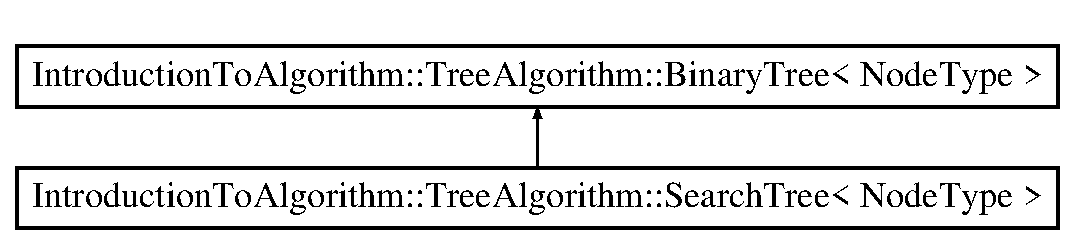
\includegraphics[height=2.000000cm]{class_introduction_to_algorithm_1_1_tree_algorithm_1_1_search_tree}
\end{center}
\end{figure}
\subsection*{Public Types}
\begin{DoxyCompactItemize}
\item 
typedef Node\+Type\+::\+Key\+Type \hyperlink{class_introduction_to_algorithm_1_1_tree_algorithm_1_1_search_tree_a0a9b2de6326042f2a1fa8a3a0def67ab}{T}
\end{DoxyCompactItemize}
\subsection*{Public Member Functions}
\begin{DoxyCompactItemize}
\item 
std\+::shared\+\_\+ptr$<$ \hyperlink{struct_introduction_to_algorithm_1_1_tree_algorithm_1_1_binary_tree_a9a441f3f41c5b69758204ba60fe02010}{Node\+Type} $>$ \hyperlink{class_introduction_to_algorithm_1_1_tree_algorithm_1_1_search_tree_affaf44d28dc2180f93669cb8d6c09c84}{search} (const \hyperlink{class_introduction_to_algorithm_1_1_tree_algorithm_1_1_search_tree_a0a9b2de6326042f2a1fa8a3a0def67ab}{T} \&value, std\+::shared\+\_\+ptr$<$ \hyperlink{struct_introduction_to_algorithm_1_1_tree_algorithm_1_1_binary_tree_a9a441f3f41c5b69758204ba60fe02010}{Node\+Type} $>$ node=std\+::shared\+\_\+ptr$<$ \hyperlink{struct_introduction_to_algorithm_1_1_tree_algorithm_1_1_binary_tree_a9a441f3f41c5b69758204ba60fe02010}{Node\+Type} $>$())
\begin{DoxyCompactList}\small\item\em search\+:在二叉搜索树中搜索指定内容的节点。 \end{DoxyCompactList}\item 
std\+::shared\+\_\+ptr$<$ \hyperlink{struct_introduction_to_algorithm_1_1_tree_algorithm_1_1_binary_tree_a9a441f3f41c5b69758204ba60fe02010}{Node\+Type} $>$ \hyperlink{class_introduction_to_algorithm_1_1_tree_algorithm_1_1_search_tree_af0bb418896808f72bb1edee55d238d55}{min} (std\+::shared\+\_\+ptr$<$ \hyperlink{struct_introduction_to_algorithm_1_1_tree_algorithm_1_1_binary_tree_a9a441f3f41c5b69758204ba60fe02010}{Node\+Type} $>$ node)
\begin{DoxyCompactList}\small\item\em min\+:在二叉搜索树中最小值的节点。 \end{DoxyCompactList}\item 
std\+::shared\+\_\+ptr$<$ \hyperlink{struct_introduction_to_algorithm_1_1_tree_algorithm_1_1_binary_tree_a9a441f3f41c5b69758204ba60fe02010}{Node\+Type} $>$ \hyperlink{class_introduction_to_algorithm_1_1_tree_algorithm_1_1_search_tree_a2dfe32f3914b03ccdb22f88f24a6afdd}{max} (std\+::shared\+\_\+ptr$<$ \hyperlink{struct_introduction_to_algorithm_1_1_tree_algorithm_1_1_binary_tree_a9a441f3f41c5b69758204ba60fe02010}{Node\+Type} $>$ node)
\begin{DoxyCompactList}\small\item\em max\+:在二叉搜索树中最大值的节点。 \end{DoxyCompactList}\item 
std\+::shared\+\_\+ptr$<$ \hyperlink{struct_introduction_to_algorithm_1_1_tree_algorithm_1_1_binary_tree_a9a441f3f41c5b69758204ba60fe02010}{Node\+Type} $>$ \hyperlink{class_introduction_to_algorithm_1_1_tree_algorithm_1_1_search_tree_a9d53e1f0b130263f2974dced515aa1f1}{successor} (std\+::shared\+\_\+ptr$<$ \hyperlink{struct_introduction_to_algorithm_1_1_tree_algorithm_1_1_binary_tree_a9a441f3f41c5b69758204ba60fe02010}{Node\+Type} $>$ node)
\begin{DoxyCompactList}\small\item\em successor\+:二叉搜索树指定节点的后继节点。 \end{DoxyCompactList}\item 
std\+::shared\+\_\+ptr$<$ \hyperlink{struct_introduction_to_algorithm_1_1_tree_algorithm_1_1_binary_tree_a9a441f3f41c5b69758204ba60fe02010}{Node\+Type} $>$ \hyperlink{class_introduction_to_algorithm_1_1_tree_algorithm_1_1_search_tree_a0e767d97590d19c97d595708d4419fe1}{predecesor} (std\+::shared\+\_\+ptr$<$ \hyperlink{struct_introduction_to_algorithm_1_1_tree_algorithm_1_1_binary_tree_a9a441f3f41c5b69758204ba60fe02010}{Node\+Type} $>$ node)
\begin{DoxyCompactList}\small\item\em predecesor\+:二叉搜索树指定节点的前驱。 \end{DoxyCompactList}\item 
void \hyperlink{class_introduction_to_algorithm_1_1_tree_algorithm_1_1_search_tree_a83724f0079d16419d4cceba74602cee1}{insert} (std\+::shared\+\_\+ptr$<$ \hyperlink{struct_introduction_to_algorithm_1_1_tree_algorithm_1_1_binary_tree_a9a441f3f41c5b69758204ba60fe02010}{Node\+Type} $>$ node)
\begin{DoxyCompactList}\small\item\em insert\+:向二叉搜索树中插入节点。 \end{DoxyCompactList}\item 
void \hyperlink{class_introduction_to_algorithm_1_1_tree_algorithm_1_1_search_tree_a3b59a0c117766590f7f01027ad0fbfff}{remove} (std\+::shared\+\_\+ptr$<$ \hyperlink{struct_introduction_to_algorithm_1_1_tree_algorithm_1_1_binary_tree_a9a441f3f41c5b69758204ba60fe02010}{Node\+Type} $>$ node)
\begin{DoxyCompactList}\small\item\em remove\+:从二叉搜索树中删除节点。 \end{DoxyCompactList}\end{DoxyCompactItemize}
\subsection*{Additional Inherited Members}


\subsection{Detailed Description}
\subsubsection*{template$<$typename Node\+Type$>$class Introduction\+To\+Algorithm\+::\+Tree\+Algorithm\+::\+Search\+Tree$<$ Node\+Type $>$}

Search\+Tree:二叉搜索树,算法导论12章 

二叉搜索树是一种特殊的二叉树。在二叉树中的任何一个节点,该节点的左子节点值小于它;该节点的右子节点值大于它。

\begin{quote}
这里节点值指的是节点存储的数据的值\end{quote}


Definition at line 33 of file searchtree.\+h.



\subsection{Member Typedef Documentation}
\hypertarget{class_introduction_to_algorithm_1_1_tree_algorithm_1_1_search_tree_a0a9b2de6326042f2a1fa8a3a0def67ab}{}\index{Introduction\+To\+Algorithm\+::\+Tree\+Algorithm\+::\+Search\+Tree@{Introduction\+To\+Algorithm\+::\+Tree\+Algorithm\+::\+Search\+Tree}!T@{T}}
\index{T@{T}!Introduction\+To\+Algorithm\+::\+Tree\+Algorithm\+::\+Search\+Tree@{Introduction\+To\+Algorithm\+::\+Tree\+Algorithm\+::\+Search\+Tree}}
\subsubsection[{T}]{\setlength{\rightskip}{0pt plus 5cm}template$<$typename Node\+Type$>$ typedef Node\+Type\+::\+Key\+Type {\bf Introduction\+To\+Algorithm\+::\+Tree\+Algorithm\+::\+Search\+Tree}$<$ {\bf Node\+Type} $>$\+::{\bf T}}\label{class_introduction_to_algorithm_1_1_tree_algorithm_1_1_search_tree_a0a9b2de6326042f2a1fa8a3a0def67ab}
树的节点存储数据的类型 

Definition at line 36 of file searchtree.\+h.



\subsection{Member Function Documentation}
\hypertarget{class_introduction_to_algorithm_1_1_tree_algorithm_1_1_search_tree_a83724f0079d16419d4cceba74602cee1}{}\index{Introduction\+To\+Algorithm\+::\+Tree\+Algorithm\+::\+Search\+Tree@{Introduction\+To\+Algorithm\+::\+Tree\+Algorithm\+::\+Search\+Tree}!insert@{insert}}
\index{insert@{insert}!Introduction\+To\+Algorithm\+::\+Tree\+Algorithm\+::\+Search\+Tree@{Introduction\+To\+Algorithm\+::\+Tree\+Algorithm\+::\+Search\+Tree}}
\subsubsection[{insert(std\+::shared\+\_\+ptr$<$ Node\+Type $>$ node)}]{\setlength{\rightskip}{0pt plus 5cm}template$<$typename Node\+Type$>$ void {\bf Introduction\+To\+Algorithm\+::\+Tree\+Algorithm\+::\+Search\+Tree}$<$ {\bf Node\+Type} $>$\+::insert (
\begin{DoxyParamCaption}
\item[{std\+::shared\+\_\+ptr$<$ {\bf Node\+Type} $>$}]{node}
\end{DoxyParamCaption}
)\hspace{0.3cm}{\ttfamily [inline]}}\label{class_introduction_to_algorithm_1_1_tree_algorithm_1_1_search_tree_a83724f0079d16419d4cceba74602cee1}


insert\+:向二叉搜索树中插入节点。 


\begin{DoxyParams}{Parameters}
{\em node\+:要插入的节点} & \\
\hline
\end{DoxyParams}
\begin{DoxyReturn}{Returns}
\+: void
\end{DoxyReturn}
给定新节点{\ttfamily node},将该节点插入到二叉搜索树中。

算法:遍历二叉搜索树,若当前节点的值大于{\ttfamily node}的值,则向左侧遍历;若当前节点值小于{\ttfamily node}的值,则向右侧遍历。直到碰到{\ttfamily nullptr}则挂载该节点

算法时间复杂度\+O(h),空间复杂度\+O(1)。其中h为树的高度 

Definition at line 191 of file searchtree.\+h.

\hypertarget{class_introduction_to_algorithm_1_1_tree_algorithm_1_1_search_tree_a2dfe32f3914b03ccdb22f88f24a6afdd}{}\index{Introduction\+To\+Algorithm\+::\+Tree\+Algorithm\+::\+Search\+Tree@{Introduction\+To\+Algorithm\+::\+Tree\+Algorithm\+::\+Search\+Tree}!max@{max}}
\index{max@{max}!Introduction\+To\+Algorithm\+::\+Tree\+Algorithm\+::\+Search\+Tree@{Introduction\+To\+Algorithm\+::\+Tree\+Algorithm\+::\+Search\+Tree}}
\subsubsection[{max(std\+::shared\+\_\+ptr$<$ Node\+Type $>$ node)}]{\setlength{\rightskip}{0pt plus 5cm}template$<$typename Node\+Type$>$ std\+::shared\+\_\+ptr$<${\bf Node\+Type}$>$ {\bf Introduction\+To\+Algorithm\+::\+Tree\+Algorithm\+::\+Search\+Tree}$<$ {\bf Node\+Type} $>$\+::max (
\begin{DoxyParamCaption}
\item[{std\+::shared\+\_\+ptr$<$ {\bf Node\+Type} $>$}]{node}
\end{DoxyParamCaption}
)\hspace{0.3cm}{\ttfamily [inline]}}\label{class_introduction_to_algorithm_1_1_tree_algorithm_1_1_search_tree_a2dfe32f3914b03ccdb22f88f24a6afdd}


max\+:在二叉搜索树中最大值的节点。 


\begin{DoxyParams}{Parameters}
{\em node\+:从指定节点开始搜索(默认为树的根节点)} & \\
\hline
\end{DoxyParams}
\begin{DoxyReturn}{Returns}
\+: 二叉树种的最大节点的强引用
\end{DoxyReturn}
在二叉搜索树中搜索最小值的节点。其中可以指定从哪个节点开始搜索。若不指定搜索节点,则默认为树的根节点

算法:由于二叉树的性质,搜索最大值很简单。从指定节点沿着右子节点一路向下遍历,最右下方的节点即为最小值节点

算法时间复杂度\+O(h),空间复杂度\+O(1)。其中h为树的高度 

Definition at line 99 of file searchtree.\+h.

\hypertarget{class_introduction_to_algorithm_1_1_tree_algorithm_1_1_search_tree_af0bb418896808f72bb1edee55d238d55}{}\index{Introduction\+To\+Algorithm\+::\+Tree\+Algorithm\+::\+Search\+Tree@{Introduction\+To\+Algorithm\+::\+Tree\+Algorithm\+::\+Search\+Tree}!min@{min}}
\index{min@{min}!Introduction\+To\+Algorithm\+::\+Tree\+Algorithm\+::\+Search\+Tree@{Introduction\+To\+Algorithm\+::\+Tree\+Algorithm\+::\+Search\+Tree}}
\subsubsection[{min(std\+::shared\+\_\+ptr$<$ Node\+Type $>$ node)}]{\setlength{\rightskip}{0pt plus 5cm}template$<$typename Node\+Type$>$ std\+::shared\+\_\+ptr$<${\bf Node\+Type}$>$ {\bf Introduction\+To\+Algorithm\+::\+Tree\+Algorithm\+::\+Search\+Tree}$<$ {\bf Node\+Type} $>$\+::min (
\begin{DoxyParamCaption}
\item[{std\+::shared\+\_\+ptr$<$ {\bf Node\+Type} $>$}]{node}
\end{DoxyParamCaption}
)\hspace{0.3cm}{\ttfamily [inline]}}\label{class_introduction_to_algorithm_1_1_tree_algorithm_1_1_search_tree_af0bb418896808f72bb1edee55d238d55}


min\+:在二叉搜索树中最小值的节点。 


\begin{DoxyParams}{Parameters}
{\em node\+:从指定节点开始搜索(默认为树的根节点)} & \\
\hline
\end{DoxyParams}
\begin{DoxyReturn}{Returns}
\+: 二叉树种的最小节点的强引用
\end{DoxyReturn}
在二叉搜索树中搜索最小值的节点。其中可以指定从哪个节点开始搜索。若不指定搜索节点,则默认为树的根节点。

算法:由于二叉树的性质,搜索最小值很简单。从指定节点沿着左子节点一路向下遍历,最左下方的节点即为最小值节点

算法时间复杂度\+O(h),空间复杂度\+O(1)。其中h为树的高度 

Definition at line 75 of file searchtree.\+h.

\hypertarget{class_introduction_to_algorithm_1_1_tree_algorithm_1_1_search_tree_a0e767d97590d19c97d595708d4419fe1}{}\index{Introduction\+To\+Algorithm\+::\+Tree\+Algorithm\+::\+Search\+Tree@{Introduction\+To\+Algorithm\+::\+Tree\+Algorithm\+::\+Search\+Tree}!predecesor@{predecesor}}
\index{predecesor@{predecesor}!Introduction\+To\+Algorithm\+::\+Tree\+Algorithm\+::\+Search\+Tree@{Introduction\+To\+Algorithm\+::\+Tree\+Algorithm\+::\+Search\+Tree}}
\subsubsection[{predecesor(std\+::shared\+\_\+ptr$<$ Node\+Type $>$ node)}]{\setlength{\rightskip}{0pt plus 5cm}template$<$typename Node\+Type$>$ std\+::shared\+\_\+ptr$<${\bf Node\+Type}$>$ {\bf Introduction\+To\+Algorithm\+::\+Tree\+Algorithm\+::\+Search\+Tree}$<$ {\bf Node\+Type} $>$\+::predecesor (
\begin{DoxyParamCaption}
\item[{std\+::shared\+\_\+ptr$<$ {\bf Node\+Type} $>$}]{node}
\end{DoxyParamCaption}
)\hspace{0.3cm}{\ttfamily [inline]}}\label{class_introduction_to_algorithm_1_1_tree_algorithm_1_1_search_tree_a0e767d97590d19c97d595708d4419fe1}


predecesor\+:二叉搜索树指定节点的前驱。 


\begin{DoxyParams}{Parameters}
{\em node\+:要搜索前驱的节点} & \\
\hline
\end{DoxyParams}
\begin{DoxyReturn}{Returns}
\+: 该节点的前驱节点的强引用或者空
\end{DoxyReturn}
给定二叉搜索树的某个节点,搜索其前驱节点。所谓的某节点{\ttfamily node}的前驱节点就是在二叉搜索树中,值小于{\ttfamily node}的所有节点中最大的那一个。

一个节点{\ttfamily node}的前驱有以下情况:


\begin{DoxyItemize}
\item 如果{\ttfamily node}有左子节点,则以左子节点为根的子树中的最大值节点就是{\ttfamily node}的前驱节点
\item 如果{\ttfamily node}没有左子节点,则查看父节点
\begin{DoxyItemize}
\item 若{\ttfamily node}是父节点的右子节点;则{\ttfamily node}的前驱节点是{\ttfamily node}的父节点
\item 若{\ttfamily node}是父节点的左子节点;则{\ttfamily node}设置为{\ttfamily node-\/$>$parent},递归向直到{\ttfamily node}是它父亲的右子节点;此时{\ttfamily node}的前驱节点是{\ttfamily node}的父节点
\end{DoxyItemize}
\end{DoxyItemize}

算法时间复杂度\+O(h),空间复杂度\+O(1)。其中h为树的高度 

Definition at line 161 of file searchtree.\+h.

\hypertarget{class_introduction_to_algorithm_1_1_tree_algorithm_1_1_search_tree_a3b59a0c117766590f7f01027ad0fbfff}{}\index{Introduction\+To\+Algorithm\+::\+Tree\+Algorithm\+::\+Search\+Tree@{Introduction\+To\+Algorithm\+::\+Tree\+Algorithm\+::\+Search\+Tree}!remove@{remove}}
\index{remove@{remove}!Introduction\+To\+Algorithm\+::\+Tree\+Algorithm\+::\+Search\+Tree@{Introduction\+To\+Algorithm\+::\+Tree\+Algorithm\+::\+Search\+Tree}}
\subsubsection[{remove(std\+::shared\+\_\+ptr$<$ Node\+Type $>$ node)}]{\setlength{\rightskip}{0pt plus 5cm}template$<$typename Node\+Type$>$ void {\bf Introduction\+To\+Algorithm\+::\+Tree\+Algorithm\+::\+Search\+Tree}$<$ {\bf Node\+Type} $>$\+::remove (
\begin{DoxyParamCaption}
\item[{std\+::shared\+\_\+ptr$<$ {\bf Node\+Type} $>$}]{node}
\end{DoxyParamCaption}
)\hspace{0.3cm}{\ttfamily [inline]}}\label{class_introduction_to_algorithm_1_1_tree_algorithm_1_1_search_tree_a3b59a0c117766590f7f01027ad0fbfff}


remove\+:从二叉搜索树中删除节点。 


\begin{DoxyParams}{Parameters}
{\em node\+:要删除的节点} & \\
\hline
\end{DoxyParams}
\begin{DoxyReturn}{Returns}
\+: void
\end{DoxyReturn}
给定节点{\ttfamily node},从二叉搜索树中删除它。如果{\ttfamily node}不在二叉搜索树中则抛出异常。

算法:


\begin{DoxyItemize}
\item 如果{\ttfamily node}是一个叶子节点:则直接删除它
\item 如果{\ttfamily node}有左子节点,但是没有右子节点:将左子剪切到{\ttfamily node}所在位置
\item 如果{\ttfamily node}有右子节点,但是没有左子节点:将右子剪切到{\ttfamily node}所在位置
\item 如果{\ttfamily node}既有左子节点,又有右子节点:首先获取{\ttfamily node}的后继节点{\ttfamily next\+\_\+node}
\begin{DoxyItemize}
\item 如果{\ttfamily next\+\_\+node}就是{\ttfamily node}的右子节点,则证明{\ttfamily next\+\_\+node}没有左子(如果{\ttfamily next\+\_\+node}有左子,则{\ttfamily node}的后继节点必然不是{\ttfamily next\+\_\+node})。 此时将{\ttfamily next\+\_\+node}剪切到{\ttfamily node}所在位置,并且将{\ttfamily node}的左子挂载到{\ttfamily next\+\_\+node}的左子
\item 如果{\ttfamily next\+\_\+node}不是{\ttfamily node}的右子节点,则{\ttfamily next\+\_\+node}必然位于{\ttfamily node}右子为根的子树中。且{\ttfamily next\+\_\+node}必然没有左子(否则{\ttfamily node}的后继节点必然不是{\ttfamily next\+\_\+node})
\begin{DoxyItemize}
\item 把{\ttfamily next\+\_\+node}的右子节点剪切到{\ttfamily next\+\_\+node}的位置
\item 将{\ttfamily next\+\_\+node}剪切到{\ttfamily node}的右子位置
\item 执行{\ttfamily next\+\_\+node}就是{\ttfamily node}的右子节点的操作
\end{DoxyItemize}
\end{DoxyItemize}
\end{DoxyItemize}

算法时间复杂度\+O(h),空间复杂度\+O(1)。其中h为树的高度 

Definition at line 250 of file searchtree.\+h.

\hypertarget{class_introduction_to_algorithm_1_1_tree_algorithm_1_1_search_tree_affaf44d28dc2180f93669cb8d6c09c84}{}\index{Introduction\+To\+Algorithm\+::\+Tree\+Algorithm\+::\+Search\+Tree@{Introduction\+To\+Algorithm\+::\+Tree\+Algorithm\+::\+Search\+Tree}!search@{search}}
\index{search@{search}!Introduction\+To\+Algorithm\+::\+Tree\+Algorithm\+::\+Search\+Tree@{Introduction\+To\+Algorithm\+::\+Tree\+Algorithm\+::\+Search\+Tree}}
\subsubsection[{search(const T \&value, std\+::shared\+\_\+ptr$<$ Node\+Type $>$ node=std\+::shared\+\_\+ptr$<$ Node\+Type $>$())}]{\setlength{\rightskip}{0pt plus 5cm}template$<$typename Node\+Type$>$ std\+::shared\+\_\+ptr$<${\bf Node\+Type}$>$ {\bf Introduction\+To\+Algorithm\+::\+Tree\+Algorithm\+::\+Search\+Tree}$<$ {\bf Node\+Type} $>$\+::search (
\begin{DoxyParamCaption}
\item[{const {\bf T} \&}]{value, }
\item[{std\+::shared\+\_\+ptr$<$ {\bf Node\+Type} $>$}]{node = {\ttfamily std\+:\+:shared\+\_\+ptr$<${\bf Node\+Type}$>$()}}
\end{DoxyParamCaption}
)\hspace{0.3cm}{\ttfamily [inline]}}\label{class_introduction_to_algorithm_1_1_tree_algorithm_1_1_search_tree_affaf44d28dc2180f93669cb8d6c09c84}


search\+:在二叉搜索树中搜索指定内容的节点。 


\begin{DoxyParams}{Parameters}
{\em value} & 搜索指定的内容 \\
\hline
{\em node\+:从指定节点开始搜索(默认为树的根节点)} & \\
\hline
\end{DoxyParams}
\begin{DoxyReturn}{Returns}
\+: 存储内容等于value的节点的强引用或者空
\end{DoxyReturn}
在二叉搜索树中搜索指定内容的节点。其中可以指定从哪个节点开始搜索。若不指定搜索节点,则默认为树的根节点.

算法时间复杂度\+O(h),空间复杂度\+O(1)。其中h为树的高度 

Definition at line 48 of file searchtree.\+h.

\hypertarget{class_introduction_to_algorithm_1_1_tree_algorithm_1_1_search_tree_a9d53e1f0b130263f2974dced515aa1f1}{}\index{Introduction\+To\+Algorithm\+::\+Tree\+Algorithm\+::\+Search\+Tree@{Introduction\+To\+Algorithm\+::\+Tree\+Algorithm\+::\+Search\+Tree}!successor@{successor}}
\index{successor@{successor}!Introduction\+To\+Algorithm\+::\+Tree\+Algorithm\+::\+Search\+Tree@{Introduction\+To\+Algorithm\+::\+Tree\+Algorithm\+::\+Search\+Tree}}
\subsubsection[{successor(std\+::shared\+\_\+ptr$<$ Node\+Type $>$ node)}]{\setlength{\rightskip}{0pt plus 5cm}template$<$typename Node\+Type$>$ std\+::shared\+\_\+ptr$<${\bf Node\+Type}$>$ {\bf Introduction\+To\+Algorithm\+::\+Tree\+Algorithm\+::\+Search\+Tree}$<$ {\bf Node\+Type} $>$\+::successor (
\begin{DoxyParamCaption}
\item[{std\+::shared\+\_\+ptr$<$ {\bf Node\+Type} $>$}]{node}
\end{DoxyParamCaption}
)\hspace{0.3cm}{\ttfamily [inline]}}\label{class_introduction_to_algorithm_1_1_tree_algorithm_1_1_search_tree_a9d53e1f0b130263f2974dced515aa1f1}


successor\+:二叉搜索树指定节点的后继节点。 


\begin{DoxyParams}{Parameters}
{\em node\+:要搜索后继的节点} & \\
\hline
\end{DoxyParams}
\begin{DoxyReturn}{Returns}
\+: 该节点的后继节点的强引用或者空
\end{DoxyReturn}
给定二叉搜索树的某个节点,搜索其后继节点。所谓的某节点{\ttfamily node}的后继节点就是在二叉搜索树中,值大于等于{\ttfamily node}的所有节点中最小的那一个(排除它自身)。

一个节点{\ttfamily node}的后继有以下情况:


\begin{DoxyItemize}
\item 如果{\ttfamily node}有右子节点,则以右子节点为根的子树中的最小值节点就是{\ttfamily node}的后继节点
\item 如果{\ttfamily node}没有右子节点,则查看父节点
\begin{DoxyItemize}
\item 若{\ttfamily node}是父节点的左子节点;则{\ttfamily node}的后继节点是{\ttfamily node}的父节点
\item 若{\ttfamily node}是父节点的右子节点;则{\ttfamily node}设置为{\ttfamily node-\/$>$parent},递归向直到{\ttfamily node}是它父亲的左子节点;此时{\ttfamily node}的后继节点是{\ttfamily node}的父节点
\end{DoxyItemize}
\end{DoxyItemize}

算法时间复杂度\+O(h),空间复杂度\+O(1)。其中h为树的高度 

Definition at line 127 of file searchtree.\+h.



The documentation for this class was generated from the following file\+:\begin{DoxyCompactItemize}
\item 
src/tree\+\_\+algorithms/searchtree/\hyperlink{searchtree_8h}{searchtree.\+h}\end{DoxyCompactItemize}

\hypertarget{class_search_tree_test}{}\section{Search\+Tree\+Test Class Reference}
\label{class_search_tree_test}\index{Search\+Tree\+Test@{Search\+Tree\+Test}}


\hyperlink{class_search_tree_test}{Search\+Tree\+Test}\+:测试类,用于为测试提供基础数据  




{\ttfamily \#include $<$searchtree\+\_\+test.\+h$>$}

Inheritance diagram for Search\+Tree\+Test\+:\begin{figure}[H]
\begin{center}
\leavevmode
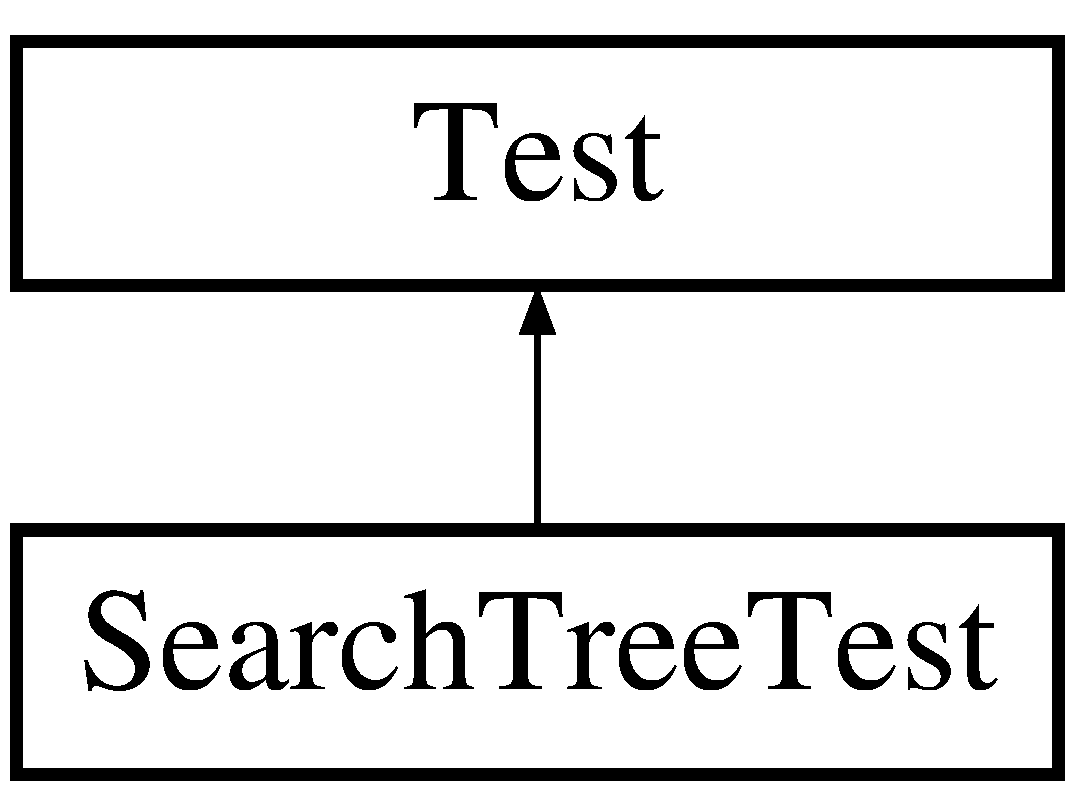
\includegraphics[height=2.000000cm]{class_search_tree_test}
\end{center}
\end{figure}
\subsection*{Public Types}
\begin{DoxyCompactItemize}
\item 
typedef \hyperlink{struct_introduction_to_algorithm_1_1_tree_algorithm_1_1_binary_tree_node}{Binary\+Tree\+Node}$<$ int $>$ \hyperlink{class_search_tree_test_a921d5813f947eb9b70417b69722bc050}{Node}
\end{DoxyCompactItemize}
\subsection*{Protected Member Functions}
\begin{DoxyCompactItemize}
\item 
\hyperlink{class_search_tree_test_a8499bee6e18b14298bb210e067d04e99}{Search\+Tree\+Test} ()
\item 
void \hyperlink{class_search_tree_test_a90a211d1322c06e96bee25849525c77f}{Set\+Up} ()
\begin{DoxyCompactList}\small\item\em Set\+Up\+:在每一个测试开始之前执行 \end{DoxyCompactList}\item 
void \hyperlink{class_search_tree_test_a2fff7db7a798909e087a66ce890f4f49}{Tear\+Down} ()
\begin{DoxyCompactList}\small\item\em Tear\+Down\+:在每一个测试结束之后执行 \end{DoxyCompactList}\end{DoxyCompactItemize}
\subsection*{Protected Attributes}
\begin{DoxyCompactItemize}
\item 
\hyperlink{class_introduction_to_algorithm_1_1_tree_algorithm_1_1_search_tree}{Search\+Tree}$<$ \hyperlink{class_search_tree_test_a921d5813f947eb9b70417b69722bc050}{Node} $>$ \hyperlink{class_search_tree_test_a08832932ab11e000dcd1ba60da8bad5f}{\+\_\+empty\+\_\+tree}
\item 
\hyperlink{class_introduction_to_algorithm_1_1_tree_algorithm_1_1_search_tree}{Search\+Tree}$<$ \hyperlink{class_search_tree_test_a921d5813f947eb9b70417b69722bc050}{Node} $>$ \hyperlink{class_search_tree_test_a9982df0c932b171ff29dfe7abcebdc05}{\+\_\+normal\+\_\+tree}
\end{DoxyCompactItemize}


\subsection{Detailed Description}
\hyperlink{class_search_tree_test}{Search\+Tree\+Test}\+:测试类,用于为测试提供基础数据 

{\ttfamily \hyperlink{class_search_tree_test}{Search\+Tree\+Test}}是 {\ttfamily \+::testing\+::\+Test} 的子类。它主要用于为每一个{\ttfamily T\+E\+S\+T\+\_\+\+F}准备测试环境 

Definition at line 45 of file searchtree\+\_\+test.\+h.



\subsection{Member Typedef Documentation}
\hypertarget{class_search_tree_test_a921d5813f947eb9b70417b69722bc050}{}\index{Search\+Tree\+Test@{Search\+Tree\+Test}!Node@{Node}}
\index{Node@{Node}!Search\+Tree\+Test@{Search\+Tree\+Test}}
\subsubsection[{Node}]{\setlength{\rightskip}{0pt plus 5cm}typedef {\bf Binary\+Tree\+Node}$<$int$>$ {\bf Search\+Tree\+Test\+::\+Node}}\label{class_search_tree_test_a921d5813f947eb9b70417b69722bc050}


Definition at line 48 of file searchtree\+\_\+test.\+h.



\subsection{Constructor \& Destructor Documentation}
\hypertarget{class_search_tree_test_a8499bee6e18b14298bb210e067d04e99}{}\index{Search\+Tree\+Test@{Search\+Tree\+Test}!Search\+Tree\+Test@{Search\+Tree\+Test}}
\index{Search\+Tree\+Test@{Search\+Tree\+Test}!Search\+Tree\+Test@{Search\+Tree\+Test}}
\subsubsection[{Search\+Tree\+Test()}]{\setlength{\rightskip}{0pt plus 5cm}Search\+Tree\+Test\+::\+Search\+Tree\+Test (
\begin{DoxyParamCaption}
{}
\end{DoxyParamCaption}
)\hspace{0.3cm}{\ttfamily [inline]}, {\ttfamily [protected]}}\label{class_search_tree_test_a8499bee6e18b14298bb210e067d04e99}


Definition at line 50 of file searchtree\+\_\+test.\+h.



\subsection{Member Function Documentation}
\hypertarget{class_search_tree_test_a90a211d1322c06e96bee25849525c77f}{}\index{Search\+Tree\+Test@{Search\+Tree\+Test}!Set\+Up@{Set\+Up}}
\index{Set\+Up@{Set\+Up}!Search\+Tree\+Test@{Search\+Tree\+Test}}
\subsubsection[{Set\+Up()}]{\setlength{\rightskip}{0pt plus 5cm}void Search\+Tree\+Test\+::\+Set\+Up (
\begin{DoxyParamCaption}
{}
\end{DoxyParamCaption}
)\hspace{0.3cm}{\ttfamily [inline]}, {\ttfamily [protected]}}\label{class_search_tree_test_a90a211d1322c06e96bee25849525c77f}


Set\+Up\+:在每一个测试开始之前执行 

{\ttfamily Set\+Up}是 {\ttfamily \+::testing\+::\+Test} 的的虚函数。它主要用于为每一个测试提供测试环境 

Definition at line 57 of file searchtree\+\_\+test.\+h.

\hypertarget{class_search_tree_test_a2fff7db7a798909e087a66ce890f4f49}{}\index{Search\+Tree\+Test@{Search\+Tree\+Test}!Tear\+Down@{Tear\+Down}}
\index{Tear\+Down@{Tear\+Down}!Search\+Tree\+Test@{Search\+Tree\+Test}}
\subsubsection[{Tear\+Down()}]{\setlength{\rightskip}{0pt plus 5cm}void Search\+Tree\+Test\+::\+Tear\+Down (
\begin{DoxyParamCaption}
{}
\end{DoxyParamCaption}
)\hspace{0.3cm}{\ttfamily [inline]}, {\ttfamily [protected]}}\label{class_search_tree_test_a2fff7db7a798909e087a66ce890f4f49}


Tear\+Down\+:在每一个测试结束之后执行 

{\ttfamily Tear\+Down}是 {\ttfamily \+::testing\+::\+Test} 的的虚函数。它主要用于为每个测试销毁测试环境 

Definition at line 97 of file searchtree\+\_\+test.\+h.



\subsection{Member Data Documentation}
\hypertarget{class_search_tree_test_a08832932ab11e000dcd1ba60da8bad5f}{}\index{Search\+Tree\+Test@{Search\+Tree\+Test}!\+\_\+empty\+\_\+tree@{\+\_\+empty\+\_\+tree}}
\index{\+\_\+empty\+\_\+tree@{\+\_\+empty\+\_\+tree}!Search\+Tree\+Test@{Search\+Tree\+Test}}
\subsubsection[{\+\_\+empty\+\_\+tree}]{\setlength{\rightskip}{0pt plus 5cm}{\bf Search\+Tree}$<${\bf Node}$>$ Search\+Tree\+Test\+::\+\_\+empty\+\_\+tree\hspace{0.3cm}{\ttfamily [protected]}}\label{class_search_tree_test_a08832932ab11e000dcd1ba60da8bad5f}
一个空的树 

Definition at line 99 of file searchtree\+\_\+test.\+h.

\hypertarget{class_search_tree_test_a9982df0c932b171ff29dfe7abcebdc05}{}\index{Search\+Tree\+Test@{Search\+Tree\+Test}!\+\_\+normal\+\_\+tree@{\+\_\+normal\+\_\+tree}}
\index{\+\_\+normal\+\_\+tree@{\+\_\+normal\+\_\+tree}!Search\+Tree\+Test@{Search\+Tree\+Test}}
\subsubsection[{\+\_\+normal\+\_\+tree}]{\setlength{\rightskip}{0pt plus 5cm}{\bf Search\+Tree}$<${\bf Node}$>$ Search\+Tree\+Test\+::\+\_\+normal\+\_\+tree\hspace{0.3cm}{\ttfamily [protected]}}\label{class_search_tree_test_a9982df0c932b171ff29dfe7abcebdc05}
一个非空的数 

Definition at line 100 of file searchtree\+\_\+test.\+h.



The documentation for this class was generated from the following file\+:\begin{DoxyCompactItemize}
\item 
src/tree\+\_\+algorithms/searchtree/\hyperlink{searchtree__test_8h}{searchtree\+\_\+test.\+h}\end{DoxyCompactItemize}

\hypertarget{struct_introduction_to_algorithm_1_1_graph_algorithm_1_1_set_vertex}{}\section{Introduction\+To\+Algorithm\+:\+:Graph\+Algorithm\+:\+:Set\+Vertex$<$ K\+Type $>$ Struct Template Reference}
\label{struct_introduction_to_algorithm_1_1_graph_algorithm_1_1_set_vertex}\index{Introduction\+To\+Algorithm\+::\+Graph\+Algorithm\+::\+Set\+Vertex$<$ K\+Type $>$@{Introduction\+To\+Algorithm\+::\+Graph\+Algorithm\+::\+Set\+Vertex$<$ K\+Type $>$}}


Set\+Vertex:图的顶点,它带一个node属性,算法导论22章22.1节  




{\ttfamily \#include $<$set\+\_\+vertex.\+h$>$}

Inheritance diagram for Introduction\+To\+Algorithm\+:\+:Graph\+Algorithm\+:\+:Set\+Vertex$<$ K\+Type $>$\+:\begin{figure}[H]
\begin{center}
\leavevmode
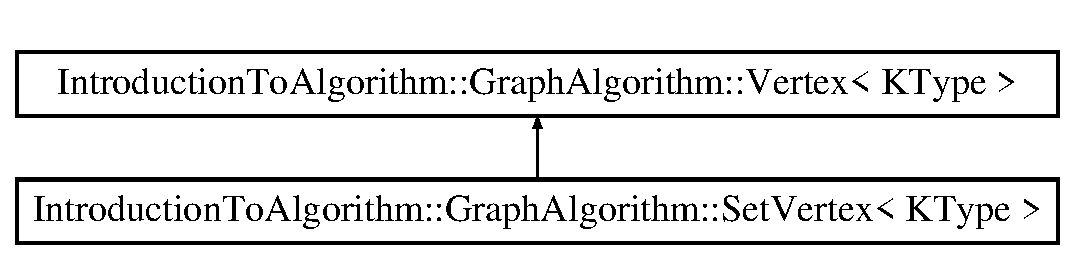
\includegraphics[height=2.000000cm]{struct_introduction_to_algorithm_1_1_graph_algorithm_1_1_set_vertex}
\end{center}
\end{figure}
\subsection*{Public Types}
\begin{DoxyCompactItemize}
\item 
typedef K\+Type \hyperlink{struct_introduction_to_algorithm_1_1_graph_algorithm_1_1_set_vertex_a0cfdcd9af991198be63495f7fb60965d}{Key\+Type}
\item 
typedef int \hyperlink{struct_introduction_to_algorithm_1_1_graph_algorithm_1_1_set_vertex_ae69791a589d95b0f4f378e08b75b041c}{V\+I\+D\+Type}
\end{DoxyCompactItemize}
\subsection*{Public Member Functions}
\begin{DoxyCompactItemize}
\item 
\hyperlink{struct_introduction_to_algorithm_1_1_graph_algorithm_1_1_set_vertex_a7a0dde758217623dbfb55598f677a4d7}{Set\+Vertex} ()
\begin{DoxyCompactList}\small\item\em 默认构造函数 \end{DoxyCompactList}\item 
\hyperlink{struct_introduction_to_algorithm_1_1_graph_algorithm_1_1_set_vertex_ae06d5b123f6a035074d270e1424ad7ec}{Set\+Vertex} (const \hyperlink{struct_introduction_to_algorithm_1_1_graph_algorithm_1_1_set_vertex_a0cfdcd9af991198be63495f7fb60965d}{Key\+Type} \&k)
\begin{DoxyCompactList}\small\item\em 显式构造函数,指定{\ttfamily key} \end{DoxyCompactList}\item 
\hyperlink{struct_introduction_to_algorithm_1_1_graph_algorithm_1_1_set_vertex_a86fd87e5d48a1b1f94ba643bd05bcc1f}{Set\+Vertex} (const \hyperlink{struct_introduction_to_algorithm_1_1_graph_algorithm_1_1_set_vertex_a0cfdcd9af991198be63495f7fb60965d}{Key\+Type} \&k, \hyperlink{struct_introduction_to_algorithm_1_1_graph_algorithm_1_1_set_vertex_ae69791a589d95b0f4f378e08b75b041c}{V\+I\+D\+Type} d)
\begin{DoxyCompactList}\small\item\em 显式构造函数,指定{\ttfamily key}和编号 \end{DoxyCompactList}\item 
virtual std\+::string \hyperlink{struct_introduction_to_algorithm_1_1_graph_algorithm_1_1_set_vertex_adb2f006ec656e2ca7c125191c601e307}{to\+\_\+string} () const 
\begin{DoxyCompactList}\small\item\em to\+\_\+string:返回顶点的字符串描述 \end{DoxyCompactList}\end{DoxyCompactItemize}
\subsection*{Public Attributes}
\begin{DoxyCompactItemize}
\item 
std\+::shared\+\_\+ptr$<$ \hyperlink{struct_introduction_to_algorithm_1_1_set_algorithm_1_1_disjoint_set_node}{Disjoint\+Set\+Node}$<$ \hyperlink{struct_introduction_to_algorithm_1_1_graph_algorithm_1_1_set_vertex}{Set\+Vertex} $>$ $>$ \hyperlink{struct_introduction_to_algorithm_1_1_graph_algorithm_1_1_set_vertex_aa01ac00440b97a31134559be597fe772}{node}
\end{DoxyCompactItemize}


\subsection{Detailed Description}
\subsubsection*{template$<$typename K\+Type$>$struct Introduction\+To\+Algorithm\+::\+Graph\+Algorithm\+::\+Set\+Vertex$<$ K\+Type $>$}

Set\+Vertex:图的顶点,它带一个node属性,算法导论22章22.1节 

它继承自\+Vertex,区别在于多了一个node成员变量,这个node是指向\+Disjoint\+Set\+Node$<$\+Set\+Vertex$>$对象的强指针。 而\+Disjoint\+Set\+Node$<$\+Set\+Vertex$>$的value成员变量是指向\+Set\+Vertex的弱指针,二者可以相互访问。 $>$Set\+Vertex没有父结点指针。要想访问\+Set\+Vertex的父结点,首先要取得它对应的\+Disjoint\+Set\+Node结点。然后获取该\+Disjoint\+Set\+Node结点的父结点。 然后通过该父结点获取value指向的\+Set\+Vertex即可。 

Definition at line 36 of file set\+\_\+vertex.\+h.



\subsection{Member Typedef Documentation}
\hypertarget{struct_introduction_to_algorithm_1_1_graph_algorithm_1_1_set_vertex_a0cfdcd9af991198be63495f7fb60965d}{}\index{Introduction\+To\+Algorithm\+::\+Graph\+Algorithm\+::\+Set\+Vertex@{Introduction\+To\+Algorithm\+::\+Graph\+Algorithm\+::\+Set\+Vertex}!Key\+Type@{Key\+Type}}
\index{Key\+Type@{Key\+Type}!Introduction\+To\+Algorithm\+::\+Graph\+Algorithm\+::\+Set\+Vertex@{Introduction\+To\+Algorithm\+::\+Graph\+Algorithm\+::\+Set\+Vertex}}
\subsubsection[{Key\+Type}]{\setlength{\rightskip}{0pt plus 5cm}template$<$typename K\+Type $>$ typedef K\+Type {\bf Introduction\+To\+Algorithm\+::\+Graph\+Algorithm\+::\+Set\+Vertex}$<$ K\+Type $>$\+::{\bf Key\+Type}}\label{struct_introduction_to_algorithm_1_1_graph_algorithm_1_1_set_vertex_a0cfdcd9af991198be63495f7fb60965d}
顶点存储数据的类型 

Definition at line 38 of file set\+\_\+vertex.\+h.

\hypertarget{struct_introduction_to_algorithm_1_1_graph_algorithm_1_1_set_vertex_ae69791a589d95b0f4f378e08b75b041c}{}\index{Introduction\+To\+Algorithm\+::\+Graph\+Algorithm\+::\+Set\+Vertex@{Introduction\+To\+Algorithm\+::\+Graph\+Algorithm\+::\+Set\+Vertex}!V\+I\+D\+Type@{V\+I\+D\+Type}}
\index{V\+I\+D\+Type@{V\+I\+D\+Type}!Introduction\+To\+Algorithm\+::\+Graph\+Algorithm\+::\+Set\+Vertex@{Introduction\+To\+Algorithm\+::\+Graph\+Algorithm\+::\+Set\+Vertex}}
\subsubsection[{V\+I\+D\+Type}]{\setlength{\rightskip}{0pt plus 5cm}template$<$typename K\+Type $>$ typedef int {\bf Introduction\+To\+Algorithm\+::\+Graph\+Algorithm\+::\+Set\+Vertex}$<$ K\+Type $>$\+::{\bf V\+I\+D\+Type}}\label{struct_introduction_to_algorithm_1_1_graph_algorithm_1_1_set_vertex_ae69791a589d95b0f4f378e08b75b041c}
顶点编号的数据类型 

Definition at line 39 of file set\+\_\+vertex.\+h.



\subsection{Constructor \& Destructor Documentation}
\hypertarget{struct_introduction_to_algorithm_1_1_graph_algorithm_1_1_set_vertex_a7a0dde758217623dbfb55598f677a4d7}{}\index{Introduction\+To\+Algorithm\+::\+Graph\+Algorithm\+::\+Set\+Vertex@{Introduction\+To\+Algorithm\+::\+Graph\+Algorithm\+::\+Set\+Vertex}!Set\+Vertex@{Set\+Vertex}}
\index{Set\+Vertex@{Set\+Vertex}!Introduction\+To\+Algorithm\+::\+Graph\+Algorithm\+::\+Set\+Vertex@{Introduction\+To\+Algorithm\+::\+Graph\+Algorithm\+::\+Set\+Vertex}}
\subsubsection[{Set\+Vertex()}]{\setlength{\rightskip}{0pt plus 5cm}template$<$typename K\+Type $>$ {\bf Introduction\+To\+Algorithm\+::\+Graph\+Algorithm\+::\+Set\+Vertex}$<$ K\+Type $>$\+::{\bf Set\+Vertex} (
\begin{DoxyParamCaption}
{}
\end{DoxyParamCaption}
)\hspace{0.3cm}{\ttfamily [inline]}}\label{struct_introduction_to_algorithm_1_1_graph_algorithm_1_1_set_vertex_a7a0dde758217623dbfb55598f677a4d7}


默认构造函数 



Definition at line 43 of file set\+\_\+vertex.\+h.

\hypertarget{struct_introduction_to_algorithm_1_1_graph_algorithm_1_1_set_vertex_ae06d5b123f6a035074d270e1424ad7ec}{}\index{Introduction\+To\+Algorithm\+::\+Graph\+Algorithm\+::\+Set\+Vertex@{Introduction\+To\+Algorithm\+::\+Graph\+Algorithm\+::\+Set\+Vertex}!Set\+Vertex@{Set\+Vertex}}
\index{Set\+Vertex@{Set\+Vertex}!Introduction\+To\+Algorithm\+::\+Graph\+Algorithm\+::\+Set\+Vertex@{Introduction\+To\+Algorithm\+::\+Graph\+Algorithm\+::\+Set\+Vertex}}
\subsubsection[{Set\+Vertex(const Key\+Type \&k)}]{\setlength{\rightskip}{0pt plus 5cm}template$<$typename K\+Type $>$ {\bf Introduction\+To\+Algorithm\+::\+Graph\+Algorithm\+::\+Set\+Vertex}$<$ K\+Type $>$\+::{\bf Set\+Vertex} (
\begin{DoxyParamCaption}
\item[{const {\bf Key\+Type} \&}]{k}
\end{DoxyParamCaption}
)\hspace{0.3cm}{\ttfamily [inline]}, {\ttfamily [explicit]}}\label{struct_introduction_to_algorithm_1_1_graph_algorithm_1_1_set_vertex_ae06d5b123f6a035074d270e1424ad7ec}


显式构造函数,指定{\ttfamily key} 


\begin{DoxyParams}{Parameters}
{\em k\+:顶点存放的数据} & \\
\hline
\end{DoxyParams}


Definition at line 48 of file set\+\_\+vertex.\+h.

\hypertarget{struct_introduction_to_algorithm_1_1_graph_algorithm_1_1_set_vertex_a86fd87e5d48a1b1f94ba643bd05bcc1f}{}\index{Introduction\+To\+Algorithm\+::\+Graph\+Algorithm\+::\+Set\+Vertex@{Introduction\+To\+Algorithm\+::\+Graph\+Algorithm\+::\+Set\+Vertex}!Set\+Vertex@{Set\+Vertex}}
\index{Set\+Vertex@{Set\+Vertex}!Introduction\+To\+Algorithm\+::\+Graph\+Algorithm\+::\+Set\+Vertex@{Introduction\+To\+Algorithm\+::\+Graph\+Algorithm\+::\+Set\+Vertex}}
\subsubsection[{Set\+Vertex(const Key\+Type \&k, V\+I\+D\+Type d)}]{\setlength{\rightskip}{0pt plus 5cm}template$<$typename K\+Type $>$ {\bf Introduction\+To\+Algorithm\+::\+Graph\+Algorithm\+::\+Set\+Vertex}$<$ K\+Type $>$\+::{\bf Set\+Vertex} (
\begin{DoxyParamCaption}
\item[{const {\bf Key\+Type} \&}]{k, }
\item[{{\bf V\+I\+D\+Type}}]{d}
\end{DoxyParamCaption}
)\hspace{0.3cm}{\ttfamily [inline]}}\label{struct_introduction_to_algorithm_1_1_graph_algorithm_1_1_set_vertex_a86fd87e5d48a1b1f94ba643bd05bcc1f}


显式构造函数,指定{\ttfamily key}和编号 


\begin{DoxyParams}{Parameters}
{\em k\+:顶点存放的数据} & \\
\hline
{\em d\+:顶点的编号} & \\
\hline
\end{DoxyParams}


Definition at line 54 of file set\+\_\+vertex.\+h.



\subsection{Member Function Documentation}
\hypertarget{struct_introduction_to_algorithm_1_1_graph_algorithm_1_1_set_vertex_adb2f006ec656e2ca7c125191c601e307}{}\index{Introduction\+To\+Algorithm\+::\+Graph\+Algorithm\+::\+Set\+Vertex@{Introduction\+To\+Algorithm\+::\+Graph\+Algorithm\+::\+Set\+Vertex}!to\+\_\+string@{to\+\_\+string}}
\index{to\+\_\+string@{to\+\_\+string}!Introduction\+To\+Algorithm\+::\+Graph\+Algorithm\+::\+Set\+Vertex@{Introduction\+To\+Algorithm\+::\+Graph\+Algorithm\+::\+Set\+Vertex}}
\subsubsection[{to\+\_\+string() const }]{\setlength{\rightskip}{0pt plus 5cm}template$<$typename K\+Type $>$ virtual std\+::string {\bf Introduction\+To\+Algorithm\+::\+Graph\+Algorithm\+::\+Set\+Vertex}$<$ K\+Type $>$\+::to\+\_\+string (
\begin{DoxyParamCaption}
{}
\end{DoxyParamCaption}
) const\hspace{0.3cm}{\ttfamily [inline]}, {\ttfamily [virtual]}}\label{struct_introduction_to_algorithm_1_1_graph_algorithm_1_1_set_vertex_adb2f006ec656e2ca7c125191c601e307}


to\+\_\+string:返回顶点的字符串描述 

\begin{DoxyReturn}{Returns}
\+:顶点的字符串描述
\end{DoxyReturn}
依次输出顶点的{\ttfamily id}、{\ttfamily key}、{\ttfamily parent}信息。 

Reimplemented from \hyperlink{struct_introduction_to_algorithm_1_1_graph_algorithm_1_1_vertex_aa8b0ab227cd3945eace9ef55f8837925}{Introduction\+To\+Algorithm\+::\+Graph\+Algorithm\+::\+Vertex$<$ K\+Type $>$}.



Definition at line 62 of file set\+\_\+vertex.\+h.



\subsection{Member Data Documentation}
\hypertarget{struct_introduction_to_algorithm_1_1_graph_algorithm_1_1_set_vertex_aa01ac00440b97a31134559be597fe772}{}\index{Introduction\+To\+Algorithm\+::\+Graph\+Algorithm\+::\+Set\+Vertex@{Introduction\+To\+Algorithm\+::\+Graph\+Algorithm\+::\+Set\+Vertex}!node@{node}}
\index{node@{node}!Introduction\+To\+Algorithm\+::\+Graph\+Algorithm\+::\+Set\+Vertex@{Introduction\+To\+Algorithm\+::\+Graph\+Algorithm\+::\+Set\+Vertex}}
\subsubsection[{node}]{\setlength{\rightskip}{0pt plus 5cm}template$<$typename K\+Type $>$ std\+::shared\+\_\+ptr$<${\bf Disjoint\+Set\+Node}$<${\bf Set\+Vertex}$>$ $>$ {\bf Introduction\+To\+Algorithm\+::\+Graph\+Algorithm\+::\+Set\+Vertex}$<$ K\+Type $>$\+::node}\label{struct_introduction_to_algorithm_1_1_graph_algorithm_1_1_set_vertex_aa01ac00440b97a31134559be597fe772}
顶点对应的\+Disjoint\+Set\+Node的强指针 

Definition at line 75 of file set\+\_\+vertex.\+h.



The documentation for this struct was generated from the following file\+:\begin{DoxyCompactItemize}
\item 
src/graph\+\_\+algorithms/basic\+\_\+graph/graph\+\_\+representation/graph\+\_\+vertex/\hyperlink{set__vertex_8h}{set\+\_\+vertex.\+h}\end{DoxyCompactItemize}

\hypertarget{class_set_vertex_test}{}\section{Set\+Vertex\+Test Class Reference}
\label{class_set_vertex_test}\index{Set\+Vertex\+Test@{Set\+Vertex\+Test}}


\hyperlink{class_set_vertex_test}{Set\+Vertex\+Test}\+:测试类,用于为测试提供基础数据  




{\ttfamily \#include $<$set\+\_\+vertex\+\_\+test.\+h$>$}

Inheritance diagram for Set\+Vertex\+Test\+:\begin{figure}[H]
\begin{center}
\leavevmode
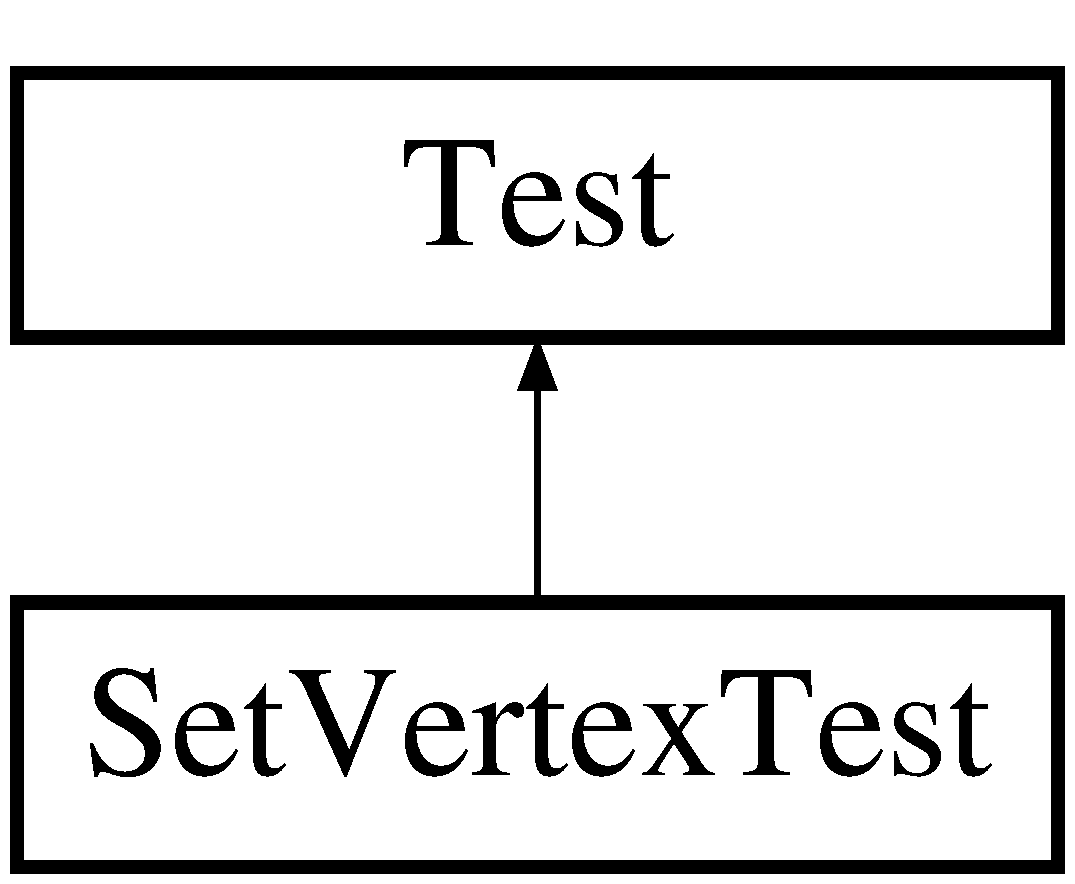
\includegraphics[height=2.000000cm]{class_set_vertex_test}
\end{center}
\end{figure}
\subsection*{Protected Member Functions}
\begin{DoxyCompactItemize}
\item 
void \hyperlink{class_set_vertex_test_a69651499454a1fea72d3ec2c4c1db15c}{Set\+Up} ()
\item 
void \hyperlink{class_set_vertex_test_a0c1de08f51a7ce42aa7cdc321715afaa}{Tear\+Down} ()
\end{DoxyCompactItemize}
\subsection*{Protected Attributes}
\begin{DoxyCompactItemize}
\item 
std\+::shared\+\_\+ptr$<$ \hyperlink{struct_introduction_to_algorithm_1_1_graph_algorithm_1_1_set_vertex}{Set\+Vertex}$<$ double $>$ $>$ \hyperlink{class_set_vertex_test_a886fbbe6fd5a4e4c954f2ff38951f90b}{\+\_\+default\+\_\+vertex}
\item 
std\+::shared\+\_\+ptr$<$ \hyperlink{struct_introduction_to_algorithm_1_1_graph_algorithm_1_1_set_vertex}{Set\+Vertex}$<$ double $>$ $>$ \hyperlink{class_set_vertex_test_af78af1aa633b65214ed39e8956beee39}{\+\_\+normal\+\_\+vertex}
\end{DoxyCompactItemize}


\subsection{Detailed Description}
\hyperlink{class_set_vertex_test}{Set\+Vertex\+Test}\+:测试类,用于为测试提供基础数据 

{\ttfamily \hyperlink{class_set_vertex_test}{Set\+Vertex\+Test}}是 {\ttfamily \+::testing\+::\+Test} 的子类。它主要用于为每一个{\ttfamily T\+E\+S\+T\+\_\+\+F}准备测试环境 

Definition at line 31 of file set\+\_\+vertex\+\_\+test.\+h.



\subsection{Member Function Documentation}
\hypertarget{class_set_vertex_test_a69651499454a1fea72d3ec2c4c1db15c}{}\index{Set\+Vertex\+Test@{Set\+Vertex\+Test}!Set\+Up@{Set\+Up}}
\index{Set\+Up@{Set\+Up}!Set\+Vertex\+Test@{Set\+Vertex\+Test}}
\subsubsection[{Set\+Up()}]{\setlength{\rightskip}{0pt plus 5cm}void Set\+Vertex\+Test\+::\+Set\+Up (
\begin{DoxyParamCaption}
{}
\end{DoxyParamCaption}
)\hspace{0.3cm}{\ttfamily [inline]}, {\ttfamily [protected]}}\label{class_set_vertex_test_a69651499454a1fea72d3ec2c4c1db15c}


Definition at line 36 of file set\+\_\+vertex\+\_\+test.\+h.

\hypertarget{class_set_vertex_test_a0c1de08f51a7ce42aa7cdc321715afaa}{}\index{Set\+Vertex\+Test@{Set\+Vertex\+Test}!Tear\+Down@{Tear\+Down}}
\index{Tear\+Down@{Tear\+Down}!Set\+Vertex\+Test@{Set\+Vertex\+Test}}
\subsubsection[{Tear\+Down()}]{\setlength{\rightskip}{0pt plus 5cm}void Set\+Vertex\+Test\+::\+Tear\+Down (
\begin{DoxyParamCaption}
{}
\end{DoxyParamCaption}
)\hspace{0.3cm}{\ttfamily [inline]}, {\ttfamily [protected]}}\label{class_set_vertex_test_a0c1de08f51a7ce42aa7cdc321715afaa}


Definition at line 41 of file set\+\_\+vertex\+\_\+test.\+h.



\subsection{Member Data Documentation}
\hypertarget{class_set_vertex_test_a886fbbe6fd5a4e4c954f2ff38951f90b}{}\index{Set\+Vertex\+Test@{Set\+Vertex\+Test}!\+\_\+default\+\_\+vertex@{\+\_\+default\+\_\+vertex}}
\index{\+\_\+default\+\_\+vertex@{\+\_\+default\+\_\+vertex}!Set\+Vertex\+Test@{Set\+Vertex\+Test}}
\subsubsection[{\+\_\+default\+\_\+vertex}]{\setlength{\rightskip}{0pt plus 5cm}std\+::shared\+\_\+ptr$<${\bf Set\+Vertex}$<$double$>$ $>$ Set\+Vertex\+Test\+::\+\_\+default\+\_\+vertex\hspace{0.3cm}{\ttfamily [protected]}}\label{class_set_vertex_test_a886fbbe6fd5a4e4c954f2ff38951f90b}
指向顶点,默认构造 

Definition at line 42 of file set\+\_\+vertex\+\_\+test.\+h.

\hypertarget{class_set_vertex_test_af78af1aa633b65214ed39e8956beee39}{}\index{Set\+Vertex\+Test@{Set\+Vertex\+Test}!\+\_\+normal\+\_\+vertex@{\+\_\+normal\+\_\+vertex}}
\index{\+\_\+normal\+\_\+vertex@{\+\_\+normal\+\_\+vertex}!Set\+Vertex\+Test@{Set\+Vertex\+Test}}
\subsubsection[{\+\_\+normal\+\_\+vertex}]{\setlength{\rightskip}{0pt plus 5cm}std\+::shared\+\_\+ptr$<${\bf Set\+Vertex}$<$double$>$ $>$ Set\+Vertex\+Test\+::\+\_\+normal\+\_\+vertex\hspace{0.3cm}{\ttfamily [protected]}}\label{class_set_vertex_test_af78af1aa633b65214ed39e8956beee39}
指向顶点,显式构造 

Definition at line 43 of file set\+\_\+vertex\+\_\+test.\+h.



The documentation for this class was generated from the following file\+:\begin{DoxyCompactItemize}
\item 
src/graph\+\_\+algorithms/basic\+\_\+graph/graph\+\_\+representation/graph\+\_\+vertex/\hyperlink{set__vertex__test_8h}{set\+\_\+vertex\+\_\+test.\+h}\end{DoxyCompactItemize}

\hypertarget{class_introduction_to_algorithm_1_1_sort_algorithm_1_1_sort___heap}{}\section{Introduction\+To\+Algorithm\+:\+:Sort\+Algorithm\+:\+:Sort\+\_\+\+Heap$<$ Iterator, Compare\+Type $>$ Class Template Reference}
\label{class_introduction_to_algorithm_1_1_sort_algorithm_1_1_sort___heap}\index{Introduction\+To\+Algorithm\+::\+Sort\+Algorithm\+::\+Sort\+\_\+\+Heap$<$ Iterator, Compare\+Type $>$@{Introduction\+To\+Algorithm\+::\+Sort\+Algorithm\+::\+Sort\+\_\+\+Heap$<$ Iterator, Compare\+Type $>$}}


Sort\+\_\+\+Heap:用于堆排序的堆,算法导论第6章  




{\ttfamily \#include $<$heapsort.\+h$>$}

\subsection*{Public Types}
\begin{DoxyCompactItemize}
\item 
typedef std\+::iterator\+\_\+traits$<$ Iterator $>$\+::value\+\_\+type \hyperlink{class_introduction_to_algorithm_1_1_sort_algorithm_1_1_sort___heap_a5af910656f5d3c65d47f992dbf380c61}{T}
\end{DoxyCompactItemize}
\subsection*{Public Member Functions}
\begin{DoxyCompactItemize}
\item 
void \hyperlink{class_introduction_to_algorithm_1_1_sort_algorithm_1_1_sort___heap_adfaf638a6fd27c6295f7ac0a07484a00}{operator()} (const Iterator from, std\+::size\+\_\+t size, Compare\+Type compare=Compare\+Type())
\begin{DoxyCompactList}\small\item\em operator() \end{DoxyCompactList}\end{DoxyCompactItemize}
\subsection*{Protected Member Functions}
\begin{DoxyCompactItemize}
\item 
void \hyperlink{class_introduction_to_algorithm_1_1_sort_algorithm_1_1_sort___heap_a64c05fac6da6e6e0d63e733640d0cf97}{\+\_\+setup\+Heap} (Compare\+Type compare=Compare\+Type())
\begin{DoxyCompactList}\small\item\em \+\_\+setup\+Heap\+:建堆 \end{DoxyCompactList}\item 
void \hyperlink{class_introduction_to_algorithm_1_1_sort_algorithm_1_1_sort___heap_a0535910130c6c750faf7801059e4a9fa}{\+\_\+heapify} (std\+::size\+\_\+t element\+Index, Compare\+Type compare=Compare\+Type())
\begin{DoxyCompactList}\small\item\em \+\_\+heapify:维持堆性质 \end{DoxyCompactList}\item 
std\+::size\+\_\+t \hyperlink{class_introduction_to_algorithm_1_1_sort_algorithm_1_1_sort___heap_a72f5fa2e41901a80fdb9a3bcece8a33f}{\+\_\+parent\+Index} (std\+::size\+\_\+t element\+Index, bool \&valid)
\begin{DoxyCompactList}\small\item\em \+\_\+parent\+Index\+:返回一个节点的父节点位置 \end{DoxyCompactList}\item 
std\+::size\+\_\+t \hyperlink{class_introduction_to_algorithm_1_1_sort_algorithm_1_1_sort___heap_af4033a3e0cd7dab78cb1081f3dece165}{\+\_\+lchild\+Index} (std\+::size\+\_\+t element\+Index, bool \&valid)
\begin{DoxyCompactList}\small\item\em \+\_\+lchild\+Index\+:返回一个节点的左子节点位置 \end{DoxyCompactList}\item 
std\+::size\+\_\+t \hyperlink{class_introduction_to_algorithm_1_1_sort_algorithm_1_1_sort___heap_a71532dbfd31fdb854aa46dbca6e411ac}{\+\_\+rchild\+Index} (std\+::size\+\_\+t element\+Index, bool \&valid)
\begin{DoxyCompactList}\small\item\em \+\_\+rchild\+Index\+:返回一个节点的右子节点位置 \end{DoxyCompactList}\end{DoxyCompactItemize}
\subsection*{Private Attributes}
\begin{DoxyCompactItemize}
\item 
Iterator \hyperlink{class_introduction_to_algorithm_1_1_sort_algorithm_1_1_sort___heap_a484d28581bfe39a387d90852e38ac36c}{\+\_\+from}
\item 
std\+::size\+\_\+t \hyperlink{class_introduction_to_algorithm_1_1_sort_algorithm_1_1_sort___heap_a57a42830d3b52d60d2ec1dfd11e2bda6}{\+\_\+size}
\end{DoxyCompactItemize}


\subsection{Detailed Description}
\subsubsection*{template$<$typename Iterator, typename Compare\+Type = std\+::less$<$typename std\+::iterator\+\_\+traits$<$\+Iterator$>$\+::value\+\_\+type$>$$>$class Introduction\+To\+Algorithm\+::\+Sort\+Algorithm\+::\+Sort\+\_\+\+Heap$<$ Iterator, Compare\+Type $>$}

Sort\+\_\+\+Heap:用于堆排序的堆,算法导论第6章 


\begin{DoxyItemize}
\item 堆排序思想:假设对数组\+A\mbox{[}p...r\mbox{]}排序:首先将数组构建成一个最大堆(或者最小堆,这里的实现采用最大堆)。然后第一个元素就是堆中最大的元素。 将第一个元素与最后一个元素交换,同时堆的规模缩减1,再将堆维持最大堆性质。不断循环最后得到一个排序好的序列
\item 时间复杂度 O(nlogn)
\item 原地排序
\end{DoxyItemize}

堆排序有两个重要操作:


\begin{DoxyItemize}
\item heapify(index)操作:维持以index为根节点的子堆的性质。它比较index与其左右子节点的值,选取其最大的那个提升到index节点上。同时递归向下。具体见\+\_\+heapify()方法说明
\item setup\+Heap()操作: 建堆操作。它从堆的最低层向上层反复调用heapify操作进行建堆。 
\end{DoxyItemize}

Definition at line 40 of file heapsort.\+h.



\subsection{Member Typedef Documentation}
\hypertarget{class_introduction_to_algorithm_1_1_sort_algorithm_1_1_sort___heap_a5af910656f5d3c65d47f992dbf380c61}{}\index{Introduction\+To\+Algorithm\+::\+Sort\+Algorithm\+::\+Sort\+\_\+\+Heap@{Introduction\+To\+Algorithm\+::\+Sort\+Algorithm\+::\+Sort\+\_\+\+Heap}!T@{T}}
\index{T@{T}!Introduction\+To\+Algorithm\+::\+Sort\+Algorithm\+::\+Sort\+\_\+\+Heap@{Introduction\+To\+Algorithm\+::\+Sort\+Algorithm\+::\+Sort\+\_\+\+Heap}}
\subsubsection[{T}]{\setlength{\rightskip}{0pt plus 5cm}template$<$typename Iterator, typename Compare\+Type = std\+::less$<$typename std\+::iterator\+\_\+traits$<$\+Iterator$>$\+::value\+\_\+type$>$$>$ typedef std\+::iterator\+\_\+traits$<$Iterator$>$\+::value\+\_\+type {\bf Introduction\+To\+Algorithm\+::\+Sort\+Algorithm\+::\+Sort\+\_\+\+Heap}$<$ Iterator, Compare\+Type $>$\+::{\bf T}}\label{class_introduction_to_algorithm_1_1_sort_algorithm_1_1_sort___heap_a5af910656f5d3c65d47f992dbf380c61}
迭代器指向对象的值类型 

Definition at line 43 of file heapsort.\+h.



\subsection{Member Function Documentation}
\hypertarget{class_introduction_to_algorithm_1_1_sort_algorithm_1_1_sort___heap_a0535910130c6c750faf7801059e4a9fa}{}\index{Introduction\+To\+Algorithm\+::\+Sort\+Algorithm\+::\+Sort\+\_\+\+Heap@{Introduction\+To\+Algorithm\+::\+Sort\+Algorithm\+::\+Sort\+\_\+\+Heap}!\+\_\+heapify@{\+\_\+heapify}}
\index{\+\_\+heapify@{\+\_\+heapify}!Introduction\+To\+Algorithm\+::\+Sort\+Algorithm\+::\+Sort\+\_\+\+Heap@{Introduction\+To\+Algorithm\+::\+Sort\+Algorithm\+::\+Sort\+\_\+\+Heap}}
\subsubsection[{\+\_\+heapify(std\+::size\+\_\+t element\+Index, Compare\+Type compare=\+Compare\+Type())}]{\setlength{\rightskip}{0pt plus 5cm}template$<$typename Iterator, typename Compare\+Type = std\+::less$<$typename std\+::iterator\+\_\+traits$<$\+Iterator$>$\+::value\+\_\+type$>$$>$ void {\bf Introduction\+To\+Algorithm\+::\+Sort\+Algorithm\+::\+Sort\+\_\+\+Heap}$<$ Iterator, Compare\+Type $>$\+::\+\_\+heapify (
\begin{DoxyParamCaption}
\item[{std\+::size\+\_\+t}]{element\+Index, }
\item[{Compare\+Type}]{compare = {\ttfamily CompareType()}}
\end{DoxyParamCaption}
)\hspace{0.3cm}{\ttfamily [inline]}, {\ttfamily [protected]}}\label{class_introduction_to_algorithm_1_1_sort_algorithm_1_1_sort___heap_a0535910130c6c750faf7801059e4a9fa}


\+\_\+heapify:维持堆性质 


\begin{DoxyParams}{Parameters}
{\em element\+Index} & \+: 要维持以该节点为根节点的子堆的堆性质 \\
\hline
{\em compare} & 一个可调用对象,可用于比较两个对象的小于比较,默认为std\+::less$<$\+T$>$ \\
\hline
\end{DoxyParams}
\begin{DoxyReturn}{Returns}
void
\end{DoxyReturn}
首先调用比较该节点与左右子节点的最大值。如果最大值为它本身,则维持了性质,返回;如果最大值不是它本身,那么必然为左、右子节点之一。 将该最大节点(假设为左子节点)交换到根节点,然后以左子节点递归调用heapify操作


\begin{DoxyItemize}
\item 时间复杂度 O(n)
\item 原地操作 
\end{DoxyItemize}

Definition at line 102 of file heapsort.\+h.

\hypertarget{class_introduction_to_algorithm_1_1_sort_algorithm_1_1_sort___heap_af4033a3e0cd7dab78cb1081f3dece165}{}\index{Introduction\+To\+Algorithm\+::\+Sort\+Algorithm\+::\+Sort\+\_\+\+Heap@{Introduction\+To\+Algorithm\+::\+Sort\+Algorithm\+::\+Sort\+\_\+\+Heap}!\+\_\+lchild\+Index@{\+\_\+lchild\+Index}}
\index{\+\_\+lchild\+Index@{\+\_\+lchild\+Index}!Introduction\+To\+Algorithm\+::\+Sort\+Algorithm\+::\+Sort\+\_\+\+Heap@{Introduction\+To\+Algorithm\+::\+Sort\+Algorithm\+::\+Sort\+\_\+\+Heap}}
\subsubsection[{\+\_\+lchild\+Index(std\+::size\+\_\+t element\+Index, bool \&valid)}]{\setlength{\rightskip}{0pt plus 5cm}template$<$typename Iterator, typename Compare\+Type = std\+::less$<$typename std\+::iterator\+\_\+traits$<$\+Iterator$>$\+::value\+\_\+type$>$$>$ std\+::size\+\_\+t {\bf Introduction\+To\+Algorithm\+::\+Sort\+Algorithm\+::\+Sort\+\_\+\+Heap}$<$ Iterator, Compare\+Type $>$\+::\+\_\+lchild\+Index (
\begin{DoxyParamCaption}
\item[{std\+::size\+\_\+t}]{element\+Index, }
\item[{bool \&}]{valid}
\end{DoxyParamCaption}
)\hspace{0.3cm}{\ttfamily [inline]}, {\ttfamily [protected]}}\label{class_introduction_to_algorithm_1_1_sort_algorithm_1_1_sort___heap_af4033a3e0cd7dab78cb1081f3dece165}


\+\_\+lchild\+Index\+:返回一个节点的左子节点位置 


\begin{DoxyParams}{Parameters}
{\em element\+Index} & \+: 节点位置 \\
\hline
{\em valid} & 一个bool\&值,用于返回,指示子节点是否有效 \\
\hline
\end{DoxyParams}
\begin{DoxyReturn}{Returns}
左子节点位置(std\+::size\+\_\+t)
\end{DoxyReturn}
根据最大堆的性质,一个节点element\+Index的左子节点是它的位置(element\+Index/2)+1


\begin{DoxyItemize}
\item 当最大堆大小为0、1时,它没有左子节点,左子节点无效
\item 当左子节点超过堆大小时,它无效 
\end{DoxyItemize}

Definition at line 162 of file heapsort.\+h.

\hypertarget{class_introduction_to_algorithm_1_1_sort_algorithm_1_1_sort___heap_a72f5fa2e41901a80fdb9a3bcece8a33f}{}\index{Introduction\+To\+Algorithm\+::\+Sort\+Algorithm\+::\+Sort\+\_\+\+Heap@{Introduction\+To\+Algorithm\+::\+Sort\+Algorithm\+::\+Sort\+\_\+\+Heap}!\+\_\+parent\+Index@{\+\_\+parent\+Index}}
\index{\+\_\+parent\+Index@{\+\_\+parent\+Index}!Introduction\+To\+Algorithm\+::\+Sort\+Algorithm\+::\+Sort\+\_\+\+Heap@{Introduction\+To\+Algorithm\+::\+Sort\+Algorithm\+::\+Sort\+\_\+\+Heap}}
\subsubsection[{\+\_\+parent\+Index(std\+::size\+\_\+t element\+Index, bool \&valid)}]{\setlength{\rightskip}{0pt plus 5cm}template$<$typename Iterator, typename Compare\+Type = std\+::less$<$typename std\+::iterator\+\_\+traits$<$\+Iterator$>$\+::value\+\_\+type$>$$>$ std\+::size\+\_\+t {\bf Introduction\+To\+Algorithm\+::\+Sort\+Algorithm\+::\+Sort\+\_\+\+Heap}$<$ Iterator, Compare\+Type $>$\+::\+\_\+parent\+Index (
\begin{DoxyParamCaption}
\item[{std\+::size\+\_\+t}]{element\+Index, }
\item[{bool \&}]{valid}
\end{DoxyParamCaption}
)\hspace{0.3cm}{\ttfamily [inline]}, {\ttfamily [protected]}}\label{class_introduction_to_algorithm_1_1_sort_algorithm_1_1_sort___heap_a72f5fa2e41901a80fdb9a3bcece8a33f}


\+\_\+parent\+Index\+:返回一个节点的父节点位置 


\begin{DoxyParams}{Parameters}
{\em element\+Index} & \+: 子节点位置 \\
\hline
{\em valid} & 一个bool\&值,用于返回,指示父节点是否有效 \\
\hline
\end{DoxyParams}
\begin{DoxyReturn}{Returns}
父节点位置(std\+::size\+\_\+t)
\end{DoxyReturn}
根据最大堆的性质,一个子节点element\+Index的父节点是它的位置(element\+Index-\/1)/2。


\begin{DoxyItemize}
\item 超出堆大小的节点,其父节点无效 
\end{DoxyItemize}

Definition at line 139 of file heapsort.\+h.

\hypertarget{class_introduction_to_algorithm_1_1_sort_algorithm_1_1_sort___heap_a71532dbfd31fdb854aa46dbca6e411ac}{}\index{Introduction\+To\+Algorithm\+::\+Sort\+Algorithm\+::\+Sort\+\_\+\+Heap@{Introduction\+To\+Algorithm\+::\+Sort\+Algorithm\+::\+Sort\+\_\+\+Heap}!\+\_\+rchild\+Index@{\+\_\+rchild\+Index}}
\index{\+\_\+rchild\+Index@{\+\_\+rchild\+Index}!Introduction\+To\+Algorithm\+::\+Sort\+Algorithm\+::\+Sort\+\_\+\+Heap@{Introduction\+To\+Algorithm\+::\+Sort\+Algorithm\+::\+Sort\+\_\+\+Heap}}
\subsubsection[{\+\_\+rchild\+Index(std\+::size\+\_\+t element\+Index, bool \&valid)}]{\setlength{\rightskip}{0pt plus 5cm}template$<$typename Iterator, typename Compare\+Type = std\+::less$<$typename std\+::iterator\+\_\+traits$<$\+Iterator$>$\+::value\+\_\+type$>$$>$ std\+::size\+\_\+t {\bf Introduction\+To\+Algorithm\+::\+Sort\+Algorithm\+::\+Sort\+\_\+\+Heap}$<$ Iterator, Compare\+Type $>$\+::\+\_\+rchild\+Index (
\begin{DoxyParamCaption}
\item[{std\+::size\+\_\+t}]{element\+Index, }
\item[{bool \&}]{valid}
\end{DoxyParamCaption}
)\hspace{0.3cm}{\ttfamily [inline]}, {\ttfamily [protected]}}\label{class_introduction_to_algorithm_1_1_sort_algorithm_1_1_sort___heap_a71532dbfd31fdb854aa46dbca6e411ac}


\+\_\+rchild\+Index\+:返回一个节点的右子节点位置 


\begin{DoxyParams}{Parameters}
{\em element\+Index} & \+: 节点位置 \\
\hline
{\em valid} & 一个bool\&值,用于返回,指示子节点是否有效 \\
\hline
\end{DoxyParams}
\begin{DoxyReturn}{Returns}
右子节点位置(std\+::size\+\_\+t)
\end{DoxyReturn}
根据最大堆的性质,一个节点element\+Index的右子节点是它的位置(element\+Index/2)+2


\begin{DoxyItemize}
\item 当最大堆大小为0、、1、2时,它没有右子节点,右子节点无效
\item 当右子节点超过堆大小时,它无效 
\end{DoxyItemize}

Definition at line 190 of file heapsort.\+h.

\hypertarget{class_introduction_to_algorithm_1_1_sort_algorithm_1_1_sort___heap_a64c05fac6da6e6e0d63e733640d0cf97}{}\index{Introduction\+To\+Algorithm\+::\+Sort\+Algorithm\+::\+Sort\+\_\+\+Heap@{Introduction\+To\+Algorithm\+::\+Sort\+Algorithm\+::\+Sort\+\_\+\+Heap}!\+\_\+setup\+Heap@{\+\_\+setup\+Heap}}
\index{\+\_\+setup\+Heap@{\+\_\+setup\+Heap}!Introduction\+To\+Algorithm\+::\+Sort\+Algorithm\+::\+Sort\+\_\+\+Heap@{Introduction\+To\+Algorithm\+::\+Sort\+Algorithm\+::\+Sort\+\_\+\+Heap}}
\subsubsection[{\+\_\+setup\+Heap(\+Compare\+Type compare=\+Compare\+Type())}]{\setlength{\rightskip}{0pt plus 5cm}template$<$typename Iterator, typename Compare\+Type = std\+::less$<$typename std\+::iterator\+\_\+traits$<$\+Iterator$>$\+::value\+\_\+type$>$$>$ void {\bf Introduction\+To\+Algorithm\+::\+Sort\+Algorithm\+::\+Sort\+\_\+\+Heap}$<$ Iterator, Compare\+Type $>$\+::\+\_\+setup\+Heap (
\begin{DoxyParamCaption}
\item[{Compare\+Type}]{compare = {\ttfamily CompareType()}}
\end{DoxyParamCaption}
)\hspace{0.3cm}{\ttfamily [inline]}, {\ttfamily [protected]}}\label{class_introduction_to_algorithm_1_1_sort_algorithm_1_1_sort___heap_a64c05fac6da6e6e0d63e733640d0cf97}


\+\_\+setup\+Heap\+:建堆 


\begin{DoxyParams}{Parameters}
{\em compare} & 一个可调用对象,可用于比较两个对象的小于比较,默认为std\+::less$<$\+T$>$ \\
\hline
\end{DoxyParams}
\begin{DoxyReturn}{Returns}
void
\end{DoxyReturn}
从后一半的元素开始依次向前调用heapify操作(根据最大堆性质,除了最底层它是完全充满的)


\begin{DoxyItemize}
\item 时间复杂度 O(nlogn)
\item 原地操作 
\end{DoxyItemize}

Definition at line 79 of file heapsort.\+h.

\hypertarget{class_introduction_to_algorithm_1_1_sort_algorithm_1_1_sort___heap_adfaf638a6fd27c6295f7ac0a07484a00}{}\index{Introduction\+To\+Algorithm\+::\+Sort\+Algorithm\+::\+Sort\+\_\+\+Heap@{Introduction\+To\+Algorithm\+::\+Sort\+Algorithm\+::\+Sort\+\_\+\+Heap}!operator()@{operator()}}
\index{operator()@{operator()}!Introduction\+To\+Algorithm\+::\+Sort\+Algorithm\+::\+Sort\+\_\+\+Heap@{Introduction\+To\+Algorithm\+::\+Sort\+Algorithm\+::\+Sort\+\_\+\+Heap}}
\subsubsection[{operator()(const Iterator from, std\+::size\+\_\+t size, Compare\+Type compare=\+Compare\+Type())}]{\setlength{\rightskip}{0pt plus 5cm}template$<$typename Iterator, typename Compare\+Type = std\+::less$<$typename std\+::iterator\+\_\+traits$<$\+Iterator$>$\+::value\+\_\+type$>$$>$ void {\bf Introduction\+To\+Algorithm\+::\+Sort\+Algorithm\+::\+Sort\+\_\+\+Heap}$<$ Iterator, Compare\+Type $>$\+::operator() (
\begin{DoxyParamCaption}
\item[{const Iterator}]{from, }
\item[{std\+::size\+\_\+t}]{size, }
\item[{Compare\+Type}]{compare = {\ttfamily CompareType()}}
\end{DoxyParamCaption}
)\hspace{0.3cm}{\ttfamily [inline]}}\label{class_introduction_to_algorithm_1_1_sort_algorithm_1_1_sort___heap_adfaf638a6fd27c6295f7ac0a07484a00}


operator() 


\begin{DoxyParams}{Parameters}
{\em from} & \+: 待排序序列的起始迭代器(也可以是指向数组中某元素的指针) \\
\hline
{\em size} & 待排序序列的长度 \\
\hline
{\em compare} & 一个可调用对象,可用于比较两个对象的小于比较,默认为std\+::less$<$\+T$>$ \\
\hline
\end{DoxyParams}
\begin{DoxyReturn}{Returns}
void
\end{DoxyReturn}
首先调用 \hyperlink{class_introduction_to_algorithm_1_1_sort_algorithm_1_1_sort___heap_a64c05fac6da6e6e0d63e733640d0cf97}{\+\_\+setup\+Heap()}建堆。然后再反复抽取最大值到堆尾部,然后维持堆的性质。


\begin{DoxyItemize}
\item 时间复杂度 O(nlogn)
\item 原地排序 
\end{DoxyItemize}

Definition at line 56 of file heapsort.\+h.



\subsection{Member Data Documentation}
\hypertarget{class_introduction_to_algorithm_1_1_sort_algorithm_1_1_sort___heap_a484d28581bfe39a387d90852e38ac36c}{}\index{Introduction\+To\+Algorithm\+::\+Sort\+Algorithm\+::\+Sort\+\_\+\+Heap@{Introduction\+To\+Algorithm\+::\+Sort\+Algorithm\+::\+Sort\+\_\+\+Heap}!\+\_\+from@{\+\_\+from}}
\index{\+\_\+from@{\+\_\+from}!Introduction\+To\+Algorithm\+::\+Sort\+Algorithm\+::\+Sort\+\_\+\+Heap@{Introduction\+To\+Algorithm\+::\+Sort\+Algorithm\+::\+Sort\+\_\+\+Heap}}
\subsubsection[{\+\_\+from}]{\setlength{\rightskip}{0pt plus 5cm}template$<$typename Iterator, typename Compare\+Type = std\+::less$<$typename std\+::iterator\+\_\+traits$<$\+Iterator$>$\+::value\+\_\+type$>$$>$ Iterator {\bf Introduction\+To\+Algorithm\+::\+Sort\+Algorithm\+::\+Sort\+\_\+\+Heap}$<$ Iterator, Compare\+Type $>$\+::\+\_\+from\hspace{0.3cm}{\ttfamily [private]}}\label{class_introduction_to_algorithm_1_1_sort_algorithm_1_1_sort___heap_a484d28581bfe39a387d90852e38ac36c}
堆根节点位置 

Definition at line 206 of file heapsort.\+h.

\hypertarget{class_introduction_to_algorithm_1_1_sort_algorithm_1_1_sort___heap_a57a42830d3b52d60d2ec1dfd11e2bda6}{}\index{Introduction\+To\+Algorithm\+::\+Sort\+Algorithm\+::\+Sort\+\_\+\+Heap@{Introduction\+To\+Algorithm\+::\+Sort\+Algorithm\+::\+Sort\+\_\+\+Heap}!\+\_\+size@{\+\_\+size}}
\index{\+\_\+size@{\+\_\+size}!Introduction\+To\+Algorithm\+::\+Sort\+Algorithm\+::\+Sort\+\_\+\+Heap@{Introduction\+To\+Algorithm\+::\+Sort\+Algorithm\+::\+Sort\+\_\+\+Heap}}
\subsubsection[{\+\_\+size}]{\setlength{\rightskip}{0pt plus 5cm}template$<$typename Iterator, typename Compare\+Type = std\+::less$<$typename std\+::iterator\+\_\+traits$<$\+Iterator$>$\+::value\+\_\+type$>$$>$ std\+::size\+\_\+t {\bf Introduction\+To\+Algorithm\+::\+Sort\+Algorithm\+::\+Sort\+\_\+\+Heap}$<$ Iterator, Compare\+Type $>$\+::\+\_\+size\hspace{0.3cm}{\ttfamily [private]}}\label{class_introduction_to_algorithm_1_1_sort_algorithm_1_1_sort___heap_a57a42830d3b52d60d2ec1dfd11e2bda6}
堆大小 

Definition at line 207 of file heapsort.\+h.



The documentation for this class was generated from the following file\+:\begin{DoxyCompactItemize}
\item 
src/sort\+\_\+algorithms/heap\+\_\+sort/\hyperlink{heapsort_8h}{heapsort.\+h}\end{DoxyCompactItemize}

\hypertarget{class_topology_sort_test}{}\section{Topology\+Sort\+Test Class Reference}
\label{class_topology_sort_test}\index{Topology\+Sort\+Test@{Topology\+Sort\+Test}}


\hyperlink{class_topology_sort_test}{Topology\+Sort\+Test}\+:测试类,用于为测试提供基础数据  




{\ttfamily \#include $<$topologysort\+\_\+test.\+h$>$}

Inheritance diagram for Topology\+Sort\+Test\+:\begin{figure}[H]
\begin{center}
\leavevmode
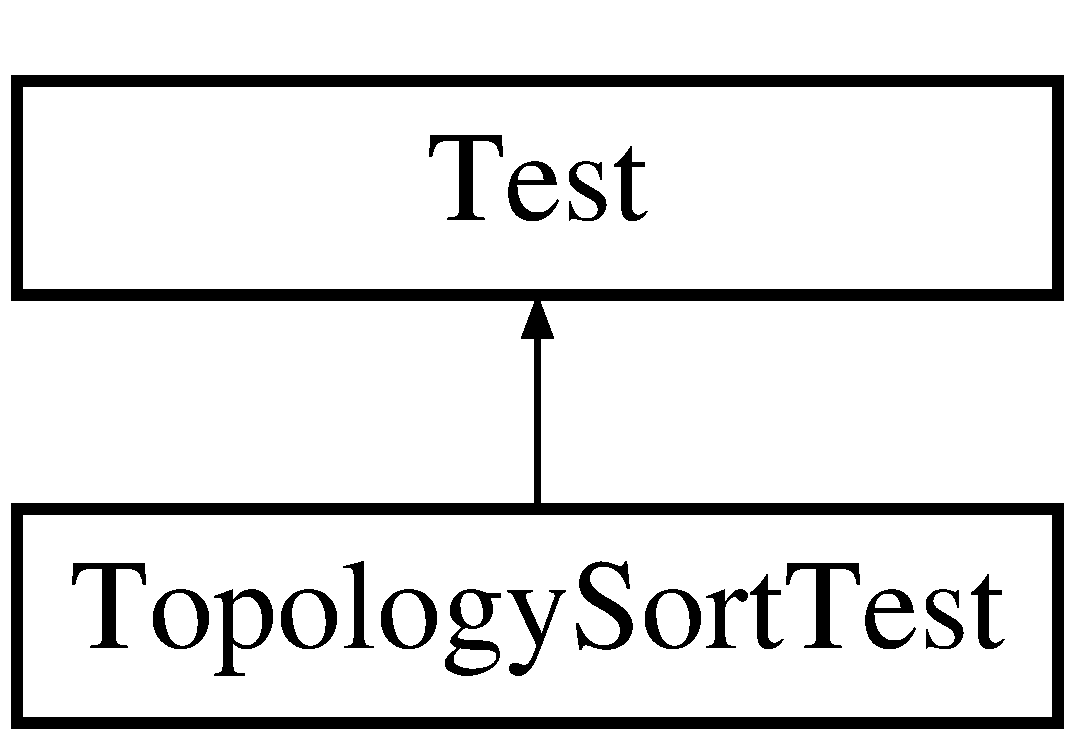
\includegraphics[height=2.000000cm]{class_topology_sort_test}
\end{center}
\end{figure}
\subsection*{Public Types}
\begin{DoxyCompactItemize}
\item 
typedef \hyperlink{struct_introduction_to_algorithm_1_1_graph_algorithm_1_1_graph}{Graph}$<$ T\+P\+S\+\_\+\+N, \hyperlink{struct_introduction_to_algorithm_1_1_graph_algorithm_1_1_d_f_s___vertex}{D\+F\+S\+\_\+\+Vertex}$<$ double $>$ $>$ \hyperlink{class_topology_sort_test_aa530f6f774d1b97dbb3968d9e445ce21}{G\+Type}
\end{DoxyCompactItemize}
\subsection*{Protected Member Functions}
\begin{DoxyCompactItemize}
\item 
void \hyperlink{class_topology_sort_test_aa1b6dad41e9cbf8b6633a355ac743957}{Set\+Up} ()
\item 
void \hyperlink{class_topology_sort_test_a1195b18b412ae18f9011d4821b50eb1f}{Tear\+Down} ()
\end{DoxyCompactItemize}
\subsection*{Protected Attributes}
\begin{DoxyCompactItemize}
\item 
std\+::shared\+\_\+ptr$<$ \hyperlink{class_topology_sort_test_aa530f6f774d1b97dbb3968d9e445ce21}{G\+Type} $>$ \hyperlink{class_topology_sort_test_a087401853f564307534465e2ac59c0ef}{\+\_\+1v\+\_\+graph}
\item 
std\+::shared\+\_\+ptr$<$ \hyperlink{class_topology_sort_test_aa530f6f774d1b97dbb3968d9e445ce21}{G\+Type} $>$ \hyperlink{class_topology_sort_test_af1fe553500cfb175b236a0302d9044af}{\+\_\+1e\+\_\+graph}
\item 
std\+::shared\+\_\+ptr$<$ \hyperlink{class_topology_sort_test_aa530f6f774d1b97dbb3968d9e445ce21}{G\+Type} $>$ \hyperlink{class_topology_sort_test_ac664dd33d2aa257a993c1835caa0d5ad}{\+\_\+list\+\_\+graph}
\end{DoxyCompactItemize}


\subsection{Detailed Description}
\hyperlink{class_topology_sort_test}{Topology\+Sort\+Test}\+:测试类,用于为测试提供基础数据 

{\ttfamily \hyperlink{class_topology_sort_test}{Topology\+Sort\+Test}}是 {\ttfamily \+::testing\+::\+Test} 的子类。它主要用于为每一个{\ttfamily T\+E\+S\+T\+\_\+\+F}准备测试环境 

Definition at line 40 of file topologysort\+\_\+test.\+h.



\subsection{Member Typedef Documentation}
\hypertarget{class_topology_sort_test_aa530f6f774d1b97dbb3968d9e445ce21}{}\index{Topology\+Sort\+Test@{Topology\+Sort\+Test}!G\+Type@{G\+Type}}
\index{G\+Type@{G\+Type}!Topology\+Sort\+Test@{Topology\+Sort\+Test}}
\subsubsection[{G\+Type}]{\setlength{\rightskip}{0pt plus 5cm}typedef {\bf Graph}$<$T\+P\+S\+\_\+\+N,{\bf D\+F\+S\+\_\+\+Vertex}$<$double$>$ $>$ {\bf Topology\+Sort\+Test\+::\+G\+Type}}\label{class_topology_sort_test_aa530f6f774d1b97dbb3968d9e445ce21}
模板实例化的图类型,该图的顶点类型为{\ttfamily D\+F\+S\+\_\+\+Vertex$<$double$>$} 

Definition at line 43 of file topologysort\+\_\+test.\+h.



\subsection{Member Function Documentation}
\hypertarget{class_topology_sort_test_aa1b6dad41e9cbf8b6633a355ac743957}{}\index{Topology\+Sort\+Test@{Topology\+Sort\+Test}!Set\+Up@{Set\+Up}}
\index{Set\+Up@{Set\+Up}!Topology\+Sort\+Test@{Topology\+Sort\+Test}}
\subsubsection[{Set\+Up()}]{\setlength{\rightskip}{0pt plus 5cm}void Topology\+Sort\+Test\+::\+Set\+Up (
\begin{DoxyParamCaption}
{}
\end{DoxyParamCaption}
)\hspace{0.3cm}{\ttfamily [inline]}, {\ttfamily [protected]}}\label{class_topology_sort_test_aa1b6dad41e9cbf8b6633a355ac743957}


Definition at line 46 of file topologysort\+\_\+test.\+h.

\hypertarget{class_topology_sort_test_a1195b18b412ae18f9011d4821b50eb1f}{}\index{Topology\+Sort\+Test@{Topology\+Sort\+Test}!Tear\+Down@{Tear\+Down}}
\index{Tear\+Down@{Tear\+Down}!Topology\+Sort\+Test@{Topology\+Sort\+Test}}
\subsubsection[{Tear\+Down()}]{\setlength{\rightskip}{0pt plus 5cm}void Topology\+Sort\+Test\+::\+Tear\+Down (
\begin{DoxyParamCaption}
{}
\end{DoxyParamCaption}
)\hspace{0.3cm}{\ttfamily [inline]}, {\ttfamily [protected]}}\label{class_topology_sort_test_a1195b18b412ae18f9011d4821b50eb1f}


Definition at line 64 of file topologysort\+\_\+test.\+h.



\subsection{Member Data Documentation}
\hypertarget{class_topology_sort_test_af1fe553500cfb175b236a0302d9044af}{}\index{Topology\+Sort\+Test@{Topology\+Sort\+Test}!\+\_\+1e\+\_\+graph@{\+\_\+1e\+\_\+graph}}
\index{\+\_\+1e\+\_\+graph@{\+\_\+1e\+\_\+graph}!Topology\+Sort\+Test@{Topology\+Sort\+Test}}
\subsubsection[{\+\_\+1e\+\_\+graph}]{\setlength{\rightskip}{0pt plus 5cm}std\+::shared\+\_\+ptr$<${\bf G\+Type}$>$ Topology\+Sort\+Test\+::\+\_\+1e\+\_\+graph\hspace{0.3cm}{\ttfamily [protected]}}\label{class_topology_sort_test_af1fe553500cfb175b236a0302d9044af}
指向一个图,该图只有一条边 

Definition at line 66 of file topologysort\+\_\+test.\+h.

\hypertarget{class_topology_sort_test_a087401853f564307534465e2ac59c0ef}{}\index{Topology\+Sort\+Test@{Topology\+Sort\+Test}!\+\_\+1v\+\_\+graph@{\+\_\+1v\+\_\+graph}}
\index{\+\_\+1v\+\_\+graph@{\+\_\+1v\+\_\+graph}!Topology\+Sort\+Test@{Topology\+Sort\+Test}}
\subsubsection[{\+\_\+1v\+\_\+graph}]{\setlength{\rightskip}{0pt plus 5cm}std\+::shared\+\_\+ptr$<${\bf G\+Type}$>$ Topology\+Sort\+Test\+::\+\_\+1v\+\_\+graph\hspace{0.3cm}{\ttfamily [protected]}}\label{class_topology_sort_test_a087401853f564307534465e2ac59c0ef}
指向一个图,该图只有一个顶点 

Definition at line 65 of file topologysort\+\_\+test.\+h.

\hypertarget{class_topology_sort_test_ac664dd33d2aa257a993c1835caa0d5ad}{}\index{Topology\+Sort\+Test@{Topology\+Sort\+Test}!\+\_\+list\+\_\+graph@{\+\_\+list\+\_\+graph}}
\index{\+\_\+list\+\_\+graph@{\+\_\+list\+\_\+graph}!Topology\+Sort\+Test@{Topology\+Sort\+Test}}
\subsubsection[{\+\_\+list\+\_\+graph}]{\setlength{\rightskip}{0pt plus 5cm}std\+::shared\+\_\+ptr$<${\bf G\+Type}$>$ Topology\+Sort\+Test\+::\+\_\+list\+\_\+graph\hspace{0.3cm}{\ttfamily [protected]}}\label{class_topology_sort_test_ac664dd33d2aa257a993c1835caa0d5ad}
指向一个图,该图的边组成一个链条 

Definition at line 67 of file topologysort\+\_\+test.\+h.



The documentation for this class was generated from the following file\+:\begin{DoxyCompactItemize}
\item 
src/graph\+\_\+algorithms/basic\+\_\+graph/topology\+\_\+sort/\hyperlink{topologysort__test_8h}{topologysort\+\_\+test.\+h}\end{DoxyCompactItemize}

\hypertarget{struct_introduction_to_algorithm_1_1_graph_algorithm_1_1_vertex}{}\section{Introduction\+To\+Algorithm\+:\+:Graph\+Algorithm\+:\+:Vertex$<$ K\+Type $>$ Struct Template Reference}
\label{struct_introduction_to_algorithm_1_1_graph_algorithm_1_1_vertex}\index{Introduction\+To\+Algorithm\+::\+Graph\+Algorithm\+::\+Vertex$<$ K\+Type $>$@{Introduction\+To\+Algorithm\+::\+Graph\+Algorithm\+::\+Vertex$<$ K\+Type $>$}}


Vertex:图的顶点,算法导论22章22.1节  




{\ttfamily \#include $<$vertex.\+h$>$}

Inheritance diagram for Introduction\+To\+Algorithm\+:\+:Graph\+Algorithm\+:\+:Vertex$<$ K\+Type $>$\+:\begin{figure}[H]
\begin{center}
\leavevmode
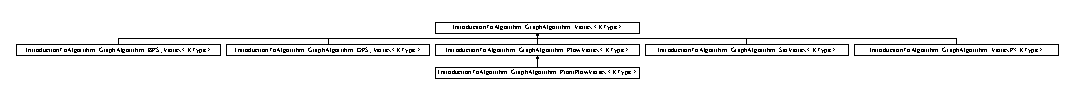
\includegraphics[height=0.825553cm]{struct_introduction_to_algorithm_1_1_graph_algorithm_1_1_vertex}
\end{center}
\end{figure}
\subsection*{Public Types}
\begin{DoxyCompactItemize}
\item 
typedef K\+Type \hyperlink{struct_introduction_to_algorithm_1_1_graph_algorithm_1_1_vertex_a14e958c58a404474853491eb811954cc}{Key\+Type}
\item 
typedef int \hyperlink{struct_introduction_to_algorithm_1_1_graph_algorithm_1_1_vertex_a290c84c0dcf159f833c72c47a2d4d44a}{V\+I\+D\+Type}
\end{DoxyCompactItemize}
\subsection*{Public Member Functions}
\begin{DoxyCompactItemize}
\item 
\hyperlink{struct_introduction_to_algorithm_1_1_graph_algorithm_1_1_vertex_a6a0b0403db78f786443e8827e6bb6af9}{Vertex} ()
\begin{DoxyCompactList}\small\item\em 默认构造函数,将{\ttfamily key}设为{\ttfamily K\+Type()},编号设为-\/1 \end{DoxyCompactList}\item 
\hyperlink{struct_introduction_to_algorithm_1_1_graph_algorithm_1_1_vertex_a047edb0a5351588129aad113a93eba54}{Vertex} (const \hyperlink{struct_introduction_to_algorithm_1_1_graph_algorithm_1_1_vertex_a14e958c58a404474853491eb811954cc}{Key\+Type} \&k)
\begin{DoxyCompactList}\small\item\em 显式构造函数,指定{\ttfamily key} \end{DoxyCompactList}\item 
\hyperlink{struct_introduction_to_algorithm_1_1_graph_algorithm_1_1_vertex_a9ed1eda4a4b48a8329acc8bd4b58150f}{Vertex} (const \hyperlink{struct_introduction_to_algorithm_1_1_graph_algorithm_1_1_vertex_a14e958c58a404474853491eb811954cc}{Key\+Type} \&k, \hyperlink{struct_introduction_to_algorithm_1_1_graph_algorithm_1_1_vertex_a290c84c0dcf159f833c72c47a2d4d44a}{V\+I\+D\+Type} d)
\begin{DoxyCompactList}\small\item\em 显式构造函数,指定{\ttfamily key}和编号 \end{DoxyCompactList}\item 
virtual std\+::string \hyperlink{struct_introduction_to_algorithm_1_1_graph_algorithm_1_1_vertex_aa8b0ab227cd3945eace9ef55f8837925}{to\+\_\+string} () const 
\begin{DoxyCompactList}\small\item\em to\+\_\+string:返回顶点的字符串描述 \end{DoxyCompactList}\end{DoxyCompactItemize}
\subsection*{Public Attributes}
\begin{DoxyCompactItemize}
\item 
\hyperlink{struct_introduction_to_algorithm_1_1_graph_algorithm_1_1_vertex_a14e958c58a404474853491eb811954cc}{Key\+Type} \hyperlink{struct_introduction_to_algorithm_1_1_graph_algorithm_1_1_vertex_a5bcfb4e0ba9450b8ebb2543069772d1f}{key}
\item 
const \hyperlink{struct_introduction_to_algorithm_1_1_graph_algorithm_1_1_vertex_a290c84c0dcf159f833c72c47a2d4d44a}{V\+I\+D\+Type} \hyperlink{struct_introduction_to_algorithm_1_1_graph_algorithm_1_1_vertex_a76668b285452856d184a245b7b35b7c1}{id}
\end{DoxyCompactItemize}


\subsection{Detailed Description}
\subsubsection*{template$<$typename K\+Type$>$struct Introduction\+To\+Algorithm\+::\+Graph\+Algorithm\+::\+Vertex$<$ K\+Type $>$}

Vertex:图的顶点,算法导论22章22.1节 

顶点是一个结构体的模板,模板类型为它存储的数据的类型。它主要包含两个数据:


\begin{DoxyItemize}
\item {\ttfamily key}\+:顶点存放的数据
\item {\ttfamily id}\+:顶点的编号(从0开始,负编号的节点为无效节点)。它是一个{\ttfamily const int},一旦顶点初始化完毕就不可更改。
\end{DoxyItemize}

默认情况下:{\ttfamily id}为-\/1,{\ttfamily key}为{\ttfamily T()}。 

Definition at line 38 of file vertex.\+h.



\subsection{Member Typedef Documentation}
\hypertarget{struct_introduction_to_algorithm_1_1_graph_algorithm_1_1_vertex_a14e958c58a404474853491eb811954cc}{}\index{Introduction\+To\+Algorithm\+::\+Graph\+Algorithm\+::\+Vertex@{Introduction\+To\+Algorithm\+::\+Graph\+Algorithm\+::\+Vertex}!Key\+Type@{Key\+Type}}
\index{Key\+Type@{Key\+Type}!Introduction\+To\+Algorithm\+::\+Graph\+Algorithm\+::\+Vertex@{Introduction\+To\+Algorithm\+::\+Graph\+Algorithm\+::\+Vertex}}
\subsubsection[{Key\+Type}]{\setlength{\rightskip}{0pt plus 5cm}template$<$typename K\+Type$>$ typedef K\+Type {\bf Introduction\+To\+Algorithm\+::\+Graph\+Algorithm\+::\+Vertex}$<$ K\+Type $>$\+::{\bf Key\+Type}}\label{struct_introduction_to_algorithm_1_1_graph_algorithm_1_1_vertex_a14e958c58a404474853491eb811954cc}
顶点存储数据的类型 

Definition at line 40 of file vertex.\+h.

\hypertarget{struct_introduction_to_algorithm_1_1_graph_algorithm_1_1_vertex_a290c84c0dcf159f833c72c47a2d4d44a}{}\index{Introduction\+To\+Algorithm\+::\+Graph\+Algorithm\+::\+Vertex@{Introduction\+To\+Algorithm\+::\+Graph\+Algorithm\+::\+Vertex}!V\+I\+D\+Type@{V\+I\+D\+Type}}
\index{V\+I\+D\+Type@{V\+I\+D\+Type}!Introduction\+To\+Algorithm\+::\+Graph\+Algorithm\+::\+Vertex@{Introduction\+To\+Algorithm\+::\+Graph\+Algorithm\+::\+Vertex}}
\subsubsection[{V\+I\+D\+Type}]{\setlength{\rightskip}{0pt plus 5cm}template$<$typename K\+Type$>$ typedef int {\bf Introduction\+To\+Algorithm\+::\+Graph\+Algorithm\+::\+Vertex}$<$ K\+Type $>$\+::{\bf V\+I\+D\+Type}}\label{struct_introduction_to_algorithm_1_1_graph_algorithm_1_1_vertex_a290c84c0dcf159f833c72c47a2d4d44a}
顶点编号的数据类型 

Definition at line 41 of file vertex.\+h.



\subsection{Constructor \& Destructor Documentation}
\hypertarget{struct_introduction_to_algorithm_1_1_graph_algorithm_1_1_vertex_a6a0b0403db78f786443e8827e6bb6af9}{}\index{Introduction\+To\+Algorithm\+::\+Graph\+Algorithm\+::\+Vertex@{Introduction\+To\+Algorithm\+::\+Graph\+Algorithm\+::\+Vertex}!Vertex@{Vertex}}
\index{Vertex@{Vertex}!Introduction\+To\+Algorithm\+::\+Graph\+Algorithm\+::\+Vertex@{Introduction\+To\+Algorithm\+::\+Graph\+Algorithm\+::\+Vertex}}
\subsubsection[{Vertex()}]{\setlength{\rightskip}{0pt plus 5cm}template$<$typename K\+Type$>$ {\bf Introduction\+To\+Algorithm\+::\+Graph\+Algorithm\+::\+Vertex}$<$ K\+Type $>$\+::{\bf Vertex} (
\begin{DoxyParamCaption}
{}
\end{DoxyParamCaption}
)\hspace{0.3cm}{\ttfamily [inline]}}\label{struct_introduction_to_algorithm_1_1_graph_algorithm_1_1_vertex_a6a0b0403db78f786443e8827e6bb6af9}


默认构造函数,将{\ttfamily key}设为{\ttfamily K\+Type()},编号设为-\/1 



Definition at line 44 of file vertex.\+h.

\hypertarget{struct_introduction_to_algorithm_1_1_graph_algorithm_1_1_vertex_a047edb0a5351588129aad113a93eba54}{}\index{Introduction\+To\+Algorithm\+::\+Graph\+Algorithm\+::\+Vertex@{Introduction\+To\+Algorithm\+::\+Graph\+Algorithm\+::\+Vertex}!Vertex@{Vertex}}
\index{Vertex@{Vertex}!Introduction\+To\+Algorithm\+::\+Graph\+Algorithm\+::\+Vertex@{Introduction\+To\+Algorithm\+::\+Graph\+Algorithm\+::\+Vertex}}
\subsubsection[{Vertex(const Key\+Type \&k)}]{\setlength{\rightskip}{0pt plus 5cm}template$<$typename K\+Type$>$ {\bf Introduction\+To\+Algorithm\+::\+Graph\+Algorithm\+::\+Vertex}$<$ K\+Type $>$\+::{\bf Vertex} (
\begin{DoxyParamCaption}
\item[{const {\bf Key\+Type} \&}]{k}
\end{DoxyParamCaption}
)\hspace{0.3cm}{\ttfamily [inline]}, {\ttfamily [explicit]}}\label{struct_introduction_to_algorithm_1_1_graph_algorithm_1_1_vertex_a047edb0a5351588129aad113a93eba54}


显式构造函数,指定{\ttfamily key} 


\begin{DoxyParams}{Parameters}
{\em k\+:顶点存放的数据} & \\
\hline
\end{DoxyParams}


Definition at line 49 of file vertex.\+h.

\hypertarget{struct_introduction_to_algorithm_1_1_graph_algorithm_1_1_vertex_a9ed1eda4a4b48a8329acc8bd4b58150f}{}\index{Introduction\+To\+Algorithm\+::\+Graph\+Algorithm\+::\+Vertex@{Introduction\+To\+Algorithm\+::\+Graph\+Algorithm\+::\+Vertex}!Vertex@{Vertex}}
\index{Vertex@{Vertex}!Introduction\+To\+Algorithm\+::\+Graph\+Algorithm\+::\+Vertex@{Introduction\+To\+Algorithm\+::\+Graph\+Algorithm\+::\+Vertex}}
\subsubsection[{Vertex(const Key\+Type \&k, V\+I\+D\+Type d)}]{\setlength{\rightskip}{0pt plus 5cm}template$<$typename K\+Type$>$ {\bf Introduction\+To\+Algorithm\+::\+Graph\+Algorithm\+::\+Vertex}$<$ K\+Type $>$\+::{\bf Vertex} (
\begin{DoxyParamCaption}
\item[{const {\bf Key\+Type} \&}]{k, }
\item[{{\bf V\+I\+D\+Type}}]{d}
\end{DoxyParamCaption}
)\hspace{0.3cm}{\ttfamily [inline]}}\label{struct_introduction_to_algorithm_1_1_graph_algorithm_1_1_vertex_a9ed1eda4a4b48a8329acc8bd4b58150f}


显式构造函数,指定{\ttfamily key}和编号 


\begin{DoxyParams}{Parameters}
{\em k\+:顶点存放的数据} & \\
\hline
{\em d\+:顶点的编号} & \\
\hline
\end{DoxyParams}


Definition at line 55 of file vertex.\+h.



\subsection{Member Function Documentation}
\hypertarget{struct_introduction_to_algorithm_1_1_graph_algorithm_1_1_vertex_aa8b0ab227cd3945eace9ef55f8837925}{}\index{Introduction\+To\+Algorithm\+::\+Graph\+Algorithm\+::\+Vertex@{Introduction\+To\+Algorithm\+::\+Graph\+Algorithm\+::\+Vertex}!to\+\_\+string@{to\+\_\+string}}
\index{to\+\_\+string@{to\+\_\+string}!Introduction\+To\+Algorithm\+::\+Graph\+Algorithm\+::\+Vertex@{Introduction\+To\+Algorithm\+::\+Graph\+Algorithm\+::\+Vertex}}
\subsubsection[{to\+\_\+string() const }]{\setlength{\rightskip}{0pt plus 5cm}template$<$typename K\+Type$>$ virtual std\+::string {\bf Introduction\+To\+Algorithm\+::\+Graph\+Algorithm\+::\+Vertex}$<$ K\+Type $>$\+::to\+\_\+string (
\begin{DoxyParamCaption}
{}
\end{DoxyParamCaption}
) const\hspace{0.3cm}{\ttfamily [inline]}, {\ttfamily [virtual]}}\label{struct_introduction_to_algorithm_1_1_graph_algorithm_1_1_vertex_aa8b0ab227cd3945eace9ef55f8837925}


to\+\_\+string:返回顶点的字符串描述 

\begin{DoxyReturn}{Returns}
\+:顶点的字符串描述
\end{DoxyReturn}
依次输出顶点的{\ttfamily id}、{\ttfamily key}信息。 

Reimplemented in \hyperlink{struct_introduction_to_algorithm_1_1_graph_algorithm_1_1_front_flow_vertex_a3edfb3a6f29475f338340291ad71eab9}{Introduction\+To\+Algorithm\+::\+Graph\+Algorithm\+::\+Front\+Flow\+Vertex$<$ K\+Type $>$}, \hyperlink{struct_introduction_to_algorithm_1_1_graph_algorithm_1_1_set_vertex_adb2f006ec656e2ca7c125191c601e307}{Introduction\+To\+Algorithm\+::\+Graph\+Algorithm\+::\+Set\+Vertex$<$ K\+Type $>$}, \hyperlink{struct_introduction_to_algorithm_1_1_graph_algorithm_1_1_flow_vertex_aa373a13a1fdee1fdcdbd0b55eaa1d1fb}{Introduction\+To\+Algorithm\+::\+Graph\+Algorithm\+::\+Flow\+Vertex$<$ K\+Type $>$}, and \hyperlink{struct_introduction_to_algorithm_1_1_graph_algorithm_1_1_vertex_p_a86c8284b603498264ea040ddb0a7065f}{Introduction\+To\+Algorithm\+::\+Graph\+Algorithm\+::\+Vertex\+P$<$ K\+Type $>$}.



Definition at line 63 of file vertex.\+h.



\subsection{Member Data Documentation}
\hypertarget{struct_introduction_to_algorithm_1_1_graph_algorithm_1_1_vertex_a76668b285452856d184a245b7b35b7c1}{}\index{Introduction\+To\+Algorithm\+::\+Graph\+Algorithm\+::\+Vertex@{Introduction\+To\+Algorithm\+::\+Graph\+Algorithm\+::\+Vertex}!id@{id}}
\index{id@{id}!Introduction\+To\+Algorithm\+::\+Graph\+Algorithm\+::\+Vertex@{Introduction\+To\+Algorithm\+::\+Graph\+Algorithm\+::\+Vertex}}
\subsubsection[{id}]{\setlength{\rightskip}{0pt plus 5cm}template$<$typename K\+Type$>$ const {\bf V\+I\+D\+Type} {\bf Introduction\+To\+Algorithm\+::\+Graph\+Algorithm\+::\+Vertex}$<$ K\+Type $>$\+::id}\label{struct_introduction_to_algorithm_1_1_graph_algorithm_1_1_vertex_a76668b285452856d184a245b7b35b7c1}
顶点id,一旦顶点生成则id不可变 

Definition at line 70 of file vertex.\+h.

\hypertarget{struct_introduction_to_algorithm_1_1_graph_algorithm_1_1_vertex_a5bcfb4e0ba9450b8ebb2543069772d1f}{}\index{Introduction\+To\+Algorithm\+::\+Graph\+Algorithm\+::\+Vertex@{Introduction\+To\+Algorithm\+::\+Graph\+Algorithm\+::\+Vertex}!key@{key}}
\index{key@{key}!Introduction\+To\+Algorithm\+::\+Graph\+Algorithm\+::\+Vertex@{Introduction\+To\+Algorithm\+::\+Graph\+Algorithm\+::\+Vertex}}
\subsubsection[{key}]{\setlength{\rightskip}{0pt plus 5cm}template$<$typename K\+Type$>$ {\bf Key\+Type} {\bf Introduction\+To\+Algorithm\+::\+Graph\+Algorithm\+::\+Vertex}$<$ K\+Type $>$\+::key}\label{struct_introduction_to_algorithm_1_1_graph_algorithm_1_1_vertex_a5bcfb4e0ba9450b8ebb2543069772d1f}
顶点存储数据 

Definition at line 69 of file vertex.\+h.



The documentation for this struct was generated from the following file\+:\begin{DoxyCompactItemize}
\item 
src/graph\+\_\+algorithms/basic\+\_\+graph/graph\+\_\+representation/graph\+\_\+vertex/\hyperlink{vertex_8h}{vertex.\+h}\end{DoxyCompactItemize}

\hypertarget{struct_introduction_to_algorithm_1_1_graph_algorithm_1_1_vertex_p}{}\section{Introduction\+To\+Algorithm\+:\+:Graph\+Algorithm\+:\+:Vertex\+P$<$ K\+Type $>$ Struct Template Reference}
\label{struct_introduction_to_algorithm_1_1_graph_algorithm_1_1_vertex_p}\index{Introduction\+To\+Algorithm\+::\+Graph\+Algorithm\+::\+Vertex\+P$<$ K\+Type $>$@{Introduction\+To\+Algorithm\+::\+Graph\+Algorithm\+::\+Vertex\+P$<$ K\+Type $>$}}


Vertex\+P:图的顶点,它带一个parent属性,算法导论22章22.1节  




{\ttfamily \#include $<$vertexp.\+h$>$}

Inheritance diagram for Introduction\+To\+Algorithm\+:\+:Graph\+Algorithm\+:\+:Vertex\+P$<$ K\+Type $>$\+:\begin{figure}[H]
\begin{center}
\leavevmode
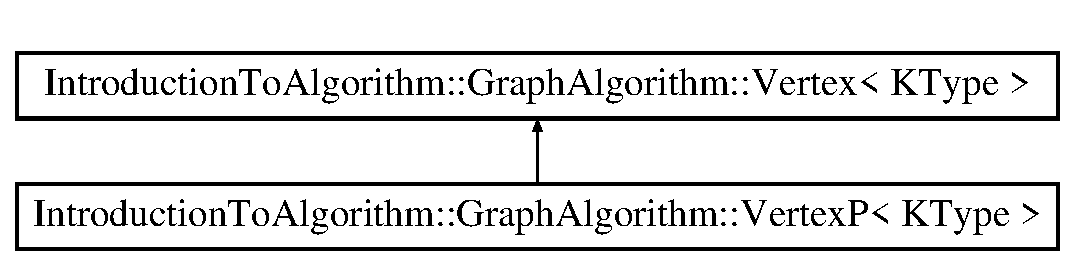
\includegraphics[height=2.000000cm]{struct_introduction_to_algorithm_1_1_graph_algorithm_1_1_vertex_p}
\end{center}
\end{figure}
\subsection*{Public Types}
\begin{DoxyCompactItemize}
\item 
typedef K\+Type \hyperlink{struct_introduction_to_algorithm_1_1_graph_algorithm_1_1_vertex_p_aa48c040b6a076ae4e1cbd5cd51f42241}{Key\+Type}
\item 
typedef int \hyperlink{struct_introduction_to_algorithm_1_1_graph_algorithm_1_1_vertex_p_aa15e0b509772ea84c9b5a211079d641b}{V\+I\+D\+Type}
\end{DoxyCompactItemize}
\subsection*{Public Member Functions}
\begin{DoxyCompactItemize}
\item 
\hyperlink{struct_introduction_to_algorithm_1_1_graph_algorithm_1_1_vertex_p_a695048962ddb2a044ff450dc17b7001e}{Vertex\+P} ()
\begin{DoxyCompactList}\small\item\em 默认构造函数 \end{DoxyCompactList}\item 
\hyperlink{struct_introduction_to_algorithm_1_1_graph_algorithm_1_1_vertex_p_afc46e0e4db66ca6dbabd85ea872d7239}{Vertex\+P} (const \hyperlink{struct_introduction_to_algorithm_1_1_graph_algorithm_1_1_vertex_a14e958c58a404474853491eb811954cc}{Key\+Type} \&k)
\begin{DoxyCompactList}\small\item\em 显式构造函数,指定{\ttfamily key} \end{DoxyCompactList}\item 
\hyperlink{struct_introduction_to_algorithm_1_1_graph_algorithm_1_1_vertex_p_aa170e385f494f36442888addfadbc711}{Vertex\+P} (const \hyperlink{struct_introduction_to_algorithm_1_1_graph_algorithm_1_1_vertex_a14e958c58a404474853491eb811954cc}{Key\+Type} \&k, \hyperlink{struct_introduction_to_algorithm_1_1_graph_algorithm_1_1_vertex_a290c84c0dcf159f833c72c47a2d4d44a}{V\+I\+D\+Type} d)
\begin{DoxyCompactList}\small\item\em 显式构造函数,指定{\ttfamily key}和编号 \end{DoxyCompactList}\item 
virtual std\+::string \hyperlink{struct_introduction_to_algorithm_1_1_graph_algorithm_1_1_vertex_p_a86c8284b603498264ea040ddb0a7065f}{to\+\_\+string} () const 
\begin{DoxyCompactList}\small\item\em to\+\_\+string:返回顶点的字符串描述 \end{DoxyCompactList}\end{DoxyCompactItemize}
\subsection*{Public Attributes}
\begin{DoxyCompactItemize}
\item 
std\+::shared\+\_\+ptr$<$ \hyperlink{struct_introduction_to_algorithm_1_1_graph_algorithm_1_1_vertex_p}{Vertex\+P} $>$ \hyperlink{struct_introduction_to_algorithm_1_1_graph_algorithm_1_1_vertex_p_ad7af59de5b07b0f26de28e9085b710ea}{parent}
\end{DoxyCompactItemize}


\subsection{Detailed Description}
\subsubsection*{template$<$typename K\+Type$>$struct Introduction\+To\+Algorithm\+::\+Graph\+Algorithm\+::\+Vertex\+P$<$ K\+Type $>$}

Vertex\+P:图的顶点,它带一个parent属性,算法导论22章22.1节 

它继承自\+Vertex,区别在于多了一个parent成员变量 

Definition at line 31 of file vertexp.\+h.



\subsection{Member Typedef Documentation}
\hypertarget{struct_introduction_to_algorithm_1_1_graph_algorithm_1_1_vertex_p_aa48c040b6a076ae4e1cbd5cd51f42241}{}\index{Introduction\+To\+Algorithm\+::\+Graph\+Algorithm\+::\+Vertex\+P@{Introduction\+To\+Algorithm\+::\+Graph\+Algorithm\+::\+Vertex\+P}!Key\+Type@{Key\+Type}}
\index{Key\+Type@{Key\+Type}!Introduction\+To\+Algorithm\+::\+Graph\+Algorithm\+::\+Vertex\+P@{Introduction\+To\+Algorithm\+::\+Graph\+Algorithm\+::\+Vertex\+P}}
\subsubsection[{Key\+Type}]{\setlength{\rightskip}{0pt plus 5cm}template$<$typename K\+Type$>$ typedef K\+Type {\bf Introduction\+To\+Algorithm\+::\+Graph\+Algorithm\+::\+Vertex\+P}$<$ K\+Type $>$\+::{\bf Key\+Type}}\label{struct_introduction_to_algorithm_1_1_graph_algorithm_1_1_vertex_p_aa48c040b6a076ae4e1cbd5cd51f42241}
顶点存储数据的类型 

Definition at line 33 of file vertexp.\+h.

\hypertarget{struct_introduction_to_algorithm_1_1_graph_algorithm_1_1_vertex_p_aa15e0b509772ea84c9b5a211079d641b}{}\index{Introduction\+To\+Algorithm\+::\+Graph\+Algorithm\+::\+Vertex\+P@{Introduction\+To\+Algorithm\+::\+Graph\+Algorithm\+::\+Vertex\+P}!V\+I\+D\+Type@{V\+I\+D\+Type}}
\index{V\+I\+D\+Type@{V\+I\+D\+Type}!Introduction\+To\+Algorithm\+::\+Graph\+Algorithm\+::\+Vertex\+P@{Introduction\+To\+Algorithm\+::\+Graph\+Algorithm\+::\+Vertex\+P}}
\subsubsection[{V\+I\+D\+Type}]{\setlength{\rightskip}{0pt plus 5cm}template$<$typename K\+Type$>$ typedef int {\bf Introduction\+To\+Algorithm\+::\+Graph\+Algorithm\+::\+Vertex\+P}$<$ K\+Type $>$\+::{\bf V\+I\+D\+Type}}\label{struct_introduction_to_algorithm_1_1_graph_algorithm_1_1_vertex_p_aa15e0b509772ea84c9b5a211079d641b}
顶点编号的数据类型 

Definition at line 34 of file vertexp.\+h.



\subsection{Constructor \& Destructor Documentation}
\hypertarget{struct_introduction_to_algorithm_1_1_graph_algorithm_1_1_vertex_p_a695048962ddb2a044ff450dc17b7001e}{}\index{Introduction\+To\+Algorithm\+::\+Graph\+Algorithm\+::\+Vertex\+P@{Introduction\+To\+Algorithm\+::\+Graph\+Algorithm\+::\+Vertex\+P}!Vertex\+P@{Vertex\+P}}
\index{Vertex\+P@{Vertex\+P}!Introduction\+To\+Algorithm\+::\+Graph\+Algorithm\+::\+Vertex\+P@{Introduction\+To\+Algorithm\+::\+Graph\+Algorithm\+::\+Vertex\+P}}
\subsubsection[{Vertex\+P()}]{\setlength{\rightskip}{0pt plus 5cm}template$<$typename K\+Type$>$ {\bf Introduction\+To\+Algorithm\+::\+Graph\+Algorithm\+::\+Vertex\+P}$<$ K\+Type $>$\+::{\bf Vertex\+P} (
\begin{DoxyParamCaption}
{}
\end{DoxyParamCaption}
)\hspace{0.3cm}{\ttfamily [inline]}}\label{struct_introduction_to_algorithm_1_1_graph_algorithm_1_1_vertex_p_a695048962ddb2a044ff450dc17b7001e}


默认构造函数 



Definition at line 37 of file vertexp.\+h.

\hypertarget{struct_introduction_to_algorithm_1_1_graph_algorithm_1_1_vertex_p_afc46e0e4db66ca6dbabd85ea872d7239}{}\index{Introduction\+To\+Algorithm\+::\+Graph\+Algorithm\+::\+Vertex\+P@{Introduction\+To\+Algorithm\+::\+Graph\+Algorithm\+::\+Vertex\+P}!Vertex\+P@{Vertex\+P}}
\index{Vertex\+P@{Vertex\+P}!Introduction\+To\+Algorithm\+::\+Graph\+Algorithm\+::\+Vertex\+P@{Introduction\+To\+Algorithm\+::\+Graph\+Algorithm\+::\+Vertex\+P}}
\subsubsection[{Vertex\+P(const Key\+Type \&k)}]{\setlength{\rightskip}{0pt plus 5cm}template$<$typename K\+Type$>$ {\bf Introduction\+To\+Algorithm\+::\+Graph\+Algorithm\+::\+Vertex\+P}$<$ K\+Type $>$\+::{\bf Vertex\+P} (
\begin{DoxyParamCaption}
\item[{const {\bf Key\+Type} \&}]{k}
\end{DoxyParamCaption}
)\hspace{0.3cm}{\ttfamily [inline]}, {\ttfamily [explicit]}}\label{struct_introduction_to_algorithm_1_1_graph_algorithm_1_1_vertex_p_afc46e0e4db66ca6dbabd85ea872d7239}


显式构造函数,指定{\ttfamily key} 


\begin{DoxyParams}{Parameters}
{\em k\+:顶点存放的数据} & \\
\hline
\end{DoxyParams}


Definition at line 42 of file vertexp.\+h.

\hypertarget{struct_introduction_to_algorithm_1_1_graph_algorithm_1_1_vertex_p_aa170e385f494f36442888addfadbc711}{}\index{Introduction\+To\+Algorithm\+::\+Graph\+Algorithm\+::\+Vertex\+P@{Introduction\+To\+Algorithm\+::\+Graph\+Algorithm\+::\+Vertex\+P}!Vertex\+P@{Vertex\+P}}
\index{Vertex\+P@{Vertex\+P}!Introduction\+To\+Algorithm\+::\+Graph\+Algorithm\+::\+Vertex\+P@{Introduction\+To\+Algorithm\+::\+Graph\+Algorithm\+::\+Vertex\+P}}
\subsubsection[{Vertex\+P(const Key\+Type \&k, V\+I\+D\+Type d)}]{\setlength{\rightskip}{0pt plus 5cm}template$<$typename K\+Type$>$ {\bf Introduction\+To\+Algorithm\+::\+Graph\+Algorithm\+::\+Vertex\+P}$<$ K\+Type $>$\+::{\bf Vertex\+P} (
\begin{DoxyParamCaption}
\item[{const {\bf Key\+Type} \&}]{k, }
\item[{{\bf V\+I\+D\+Type}}]{d}
\end{DoxyParamCaption}
)\hspace{0.3cm}{\ttfamily [inline]}}\label{struct_introduction_to_algorithm_1_1_graph_algorithm_1_1_vertex_p_aa170e385f494f36442888addfadbc711}


显式构造函数,指定{\ttfamily key}和编号 


\begin{DoxyParams}{Parameters}
{\em k\+:顶点存放的数据} & \\
\hline
{\em d\+:顶点的编号} & \\
\hline
\end{DoxyParams}


Definition at line 48 of file vertexp.\+h.



\subsection{Member Function Documentation}
\hypertarget{struct_introduction_to_algorithm_1_1_graph_algorithm_1_1_vertex_p_a86c8284b603498264ea040ddb0a7065f}{}\index{Introduction\+To\+Algorithm\+::\+Graph\+Algorithm\+::\+Vertex\+P@{Introduction\+To\+Algorithm\+::\+Graph\+Algorithm\+::\+Vertex\+P}!to\+\_\+string@{to\+\_\+string}}
\index{to\+\_\+string@{to\+\_\+string}!Introduction\+To\+Algorithm\+::\+Graph\+Algorithm\+::\+Vertex\+P@{Introduction\+To\+Algorithm\+::\+Graph\+Algorithm\+::\+Vertex\+P}}
\subsubsection[{to\+\_\+string() const }]{\setlength{\rightskip}{0pt plus 5cm}template$<$typename K\+Type$>$ virtual std\+::string {\bf Introduction\+To\+Algorithm\+::\+Graph\+Algorithm\+::\+Vertex\+P}$<$ K\+Type $>$\+::to\+\_\+string (
\begin{DoxyParamCaption}
{}
\end{DoxyParamCaption}
) const\hspace{0.3cm}{\ttfamily [inline]}, {\ttfamily [virtual]}}\label{struct_introduction_to_algorithm_1_1_graph_algorithm_1_1_vertex_p_a86c8284b603498264ea040ddb0a7065f}


to\+\_\+string:返回顶点的字符串描述 

\begin{DoxyReturn}{Returns}
\+:顶点的字符串描述
\end{DoxyReturn}
依次输出顶点的{\ttfamily id}、{\ttfamily key}、{\ttfamily parent}信息。 

Reimplemented from \hyperlink{struct_introduction_to_algorithm_1_1_graph_algorithm_1_1_vertex_aa8b0ab227cd3945eace9ef55f8837925}{Introduction\+To\+Algorithm\+::\+Graph\+Algorithm\+::\+Vertex$<$ K\+Type $>$}.



Definition at line 56 of file vertexp.\+h.



\subsection{Member Data Documentation}
\hypertarget{struct_introduction_to_algorithm_1_1_graph_algorithm_1_1_vertex_p_ad7af59de5b07b0f26de28e9085b710ea}{}\index{Introduction\+To\+Algorithm\+::\+Graph\+Algorithm\+::\+Vertex\+P@{Introduction\+To\+Algorithm\+::\+Graph\+Algorithm\+::\+Vertex\+P}!parent@{parent}}
\index{parent@{parent}!Introduction\+To\+Algorithm\+::\+Graph\+Algorithm\+::\+Vertex\+P@{Introduction\+To\+Algorithm\+::\+Graph\+Algorithm\+::\+Vertex\+P}}
\subsubsection[{parent}]{\setlength{\rightskip}{0pt plus 5cm}template$<$typename K\+Type$>$ std\+::shared\+\_\+ptr$<${\bf Vertex\+P}$>$ {\bf Introduction\+To\+Algorithm\+::\+Graph\+Algorithm\+::\+Vertex\+P}$<$ K\+Type $>$\+::parent}\label{struct_introduction_to_algorithm_1_1_graph_algorithm_1_1_vertex_p_ad7af59de5b07b0f26de28e9085b710ea}
顶点的父顶点的强指针 

Definition at line 64 of file vertexp.\+h.



The documentation for this struct was generated from the following file\+:\begin{DoxyCompactItemize}
\item 
src/graph\+\_\+algorithms/basic\+\_\+graph/graph\+\_\+representation/graph\+\_\+vertex/\hyperlink{vertexp_8h}{vertexp.\+h}\end{DoxyCompactItemize}

\chapter{File Documentation}
\hypertarget{longest__common__subsequence_8h}{}\section{src/dynamic\+\_\+programming\+\_\+algorithms/lcs/longest\+\_\+common\+\_\+subsequence.h File Reference}
\label{longest__common__subsequence_8h}\index{src/dynamic\+\_\+programming\+\_\+algorithms/lcs/longest\+\_\+common\+\_\+subsequence.\+h@{src/dynamic\+\_\+programming\+\_\+algorithms/lcs/longest\+\_\+common\+\_\+subsequence.\+h}}
{\ttfamily \#include $<$type\+\_\+traits$>$}\\*
{\ttfamily \#include $<$vector$>$}\\*
{\ttfamily \#include $<$iostream$>$}\\*
\subsection*{Namespaces}
\begin{DoxyCompactItemize}
\item 
 \hyperlink{namespace_introduction_to_algorithm}{Introduction\+To\+Algorithm}
\begin{DoxyCompactList}\small\item\em Namespace of Introdunction\+To\+Algorithm. \end{DoxyCompactList}\item 
 \hyperlink{namespace_introduction_to_algorithm_1_1_dynamic_programming_algorithm}{Introduction\+To\+Algorithm\+::\+Dynamic\+Programming\+Algorithm}
\begin{DoxyCompactList}\small\item\em Namespace of \hyperlink{namespace_introduction_to_algorithm_1_1_dynamic_programming_algorithm}{Dynamic\+Programming\+Algorithm}. \end{DoxyCompactList}\end{DoxyCompactItemize}
\subsection*{Functions}
\begin{DoxyCompactItemize}
\item 
{\footnotesize template$<$typename Iterator , typename Out\+Iterator $>$ }\\std\+::size\+\_\+t \hyperlink{namespace_introduction_to_algorithm_1_1_dynamic_programming_algorithm_a377ef4206d4814024272c15c51051f09}{Introduction\+To\+Algorithm\+::\+Dynamic\+Programming\+Algorithm\+::make\+\_\+\+L\+C\+S} (const Iterator begin, const Iterator end, const std\+::vector$<$ std\+::vector$<$ int $>$$>$ \&flag\+\_\+matrix, typename std\+::iterator\+\_\+traits$<$ Iterator $>$\+::difference\+\_\+type seq1\+\_\+index, typename std\+::iterator\+\_\+traits$<$ Iterator $>$\+::difference\+\_\+type seq2\+\_\+index, Out\+Iterator \&out\+\_\+begin)
\begin{DoxyCompactList}\small\item\em make\+\_\+\+L\+C\+S 最长公共子序列的子算法:已知标记矩阵,求最长公共子序列 \end{DoxyCompactList}\item 
{\footnotesize template$<$typename Iterator1 , typename Iterator2 , typename Out\+Iterator $>$ }\\std\+::size\+\_\+t \hyperlink{namespace_introduction_to_algorithm_1_1_dynamic_programming_algorithm_a02edd40c3c2dd3ce1b514284dd42e99c}{Introduction\+To\+Algorithm\+::\+Dynamic\+Programming\+Algorithm\+::longest\+\_\+common\+\_\+subsequence} (const Iterator1 first\+\_\+begin, const Iterator1 first\+\_\+end, const Iterator2 second\+\_\+begin, const Iterator2 second\+\_\+end, Out\+Iterator out\+\_\+begin)
\begin{DoxyCompactList}\small\item\em longest\+\_\+common\+\_\+subsequence 算法导论第15章9.4 最长公共子序列 \end{DoxyCompactList}\end{DoxyCompactItemize}

\hypertarget{longest__common__subsequence__test_8h}{}\section{src/dynamic\+\_\+programming\+\_\+algorithms/lcs/longest\+\_\+common\+\_\+subsequence\+\_\+test.h File Reference}
\label{longest__common__subsequence__test_8h}\index{src/dynamic\+\_\+programming\+\_\+algorithms/lcs/longest\+\_\+common\+\_\+subsequence\+\_\+test.\+h@{src/dynamic\+\_\+programming\+\_\+algorithms/lcs/longest\+\_\+common\+\_\+subsequence\+\_\+test.\+h}}
{\ttfamily \#include \char`\"{}src/google\+\_\+test/gtest.\+h\char`\"{}}\\*
{\ttfamily \#include \char`\"{}longest\+\_\+common\+\_\+subsequence.\+h\char`\"{}}\\*
\subsection*{Functions}
\begin{DoxyCompactItemize}
\item 
\hyperlink{longest__common__subsequence__test_8h_af6d25933a23afb7fa7f99323fe0808ea}{T\+E\+S\+T} (test\+\_\+longest\+\_\+common\+\_\+subsequence, test1)
\begin{DoxyCompactList}\small\item\em longest\+\_\+common\+\_\+subsequence\+\_\+test:测试最长公共子数组 \end{DoxyCompactList}\end{DoxyCompactItemize}


\subsection{Function Documentation}
\hypertarget{longest__common__subsequence__test_8h_af6d25933a23afb7fa7f99323fe0808ea}{}\index{longest\+\_\+common\+\_\+subsequence\+\_\+test.\+h@{longest\+\_\+common\+\_\+subsequence\+\_\+test.\+h}!T\+E\+S\+T@{T\+E\+S\+T}}
\index{T\+E\+S\+T@{T\+E\+S\+T}!longest\+\_\+common\+\_\+subsequence\+\_\+test.\+h@{longest\+\_\+common\+\_\+subsequence\+\_\+test.\+h}}
\subsubsection[{T\+E\+S\+T(test\+\_\+longest\+\_\+common\+\_\+subsequence, test1)}]{\setlength{\rightskip}{0pt plus 5cm}T\+E\+S\+T (
\begin{DoxyParamCaption}
\item[{test\+\_\+longest\+\_\+common\+\_\+subsequence}]{, }
\item[{test1}]{}
\end{DoxyParamCaption}
)}\label{longest__common__subsequence__test_8h_af6d25933a23afb7fa7f99323fe0808ea}


longest\+\_\+common\+\_\+subsequence\+\_\+test:测试最长公共子数组 

三组数据: s1为空字符串s2为非空字符串、s1和s2为常规字符串且二者内容不等、s1和s2为常规字符串且二者内容相等 

Definition at line 30 of file longest\+\_\+common\+\_\+subsequence\+\_\+test.\+h.


\hypertarget{floyd__warshall_8h}{}\section{src/graph\+\_\+algorithms/all\+\_\+node\+\_\+pair\+\_\+shortest\+\_\+path/floyd\+\_\+warshall/floyd\+\_\+warshall.h File Reference}
\label{floyd__warshall_8h}\index{src/graph\+\_\+algorithms/all\+\_\+node\+\_\+pair\+\_\+shortest\+\_\+path/floyd\+\_\+warshall/floyd\+\_\+warshall.\+h@{src/graph\+\_\+algorithms/all\+\_\+node\+\_\+pair\+\_\+shortest\+\_\+path/floyd\+\_\+warshall/floyd\+\_\+warshall.\+h}}
{\ttfamily \#include $<$memory$>$}\\*
{\ttfamily \#include \char`\"{}src/header.\+h\char`\"{}}\\*
\subsection*{Namespaces}
\begin{DoxyCompactItemize}
\item 
 \hyperlink{namespace_introduction_to_algorithm}{Introduction\+To\+Algorithm}
\begin{DoxyCompactList}\small\item\em Namespace of Introdunction\+To\+Algorithm. \end{DoxyCompactList}\item 
 \hyperlink{namespace_introduction_to_algorithm_1_1_graph_algorithm}{Introduction\+To\+Algorithm\+::\+Graph\+Algorithm}
\begin{DoxyCompactList}\small\item\em Namespace of \hyperlink{namespace_introduction_to_algorithm_1_1_graph_algorithm}{Graph\+Algorithm}. \end{DoxyCompactList}\end{DoxyCompactItemize}
\subsection*{Functions}
\begin{DoxyCompactItemize}
\item 
{\footnotesize template$<$typename Graph\+Type $>$ }\\std\+::pair$<$ std\+::array$<$ std\+::array$<$ typename Graph\+Type\+::\+E\+Weight\+Type,Graph\+Type\+::\+N\+U\+M $>$, Graph\+Type\+::\+N\+U\+M $>$, std\+::array$<$ std\+::array$<$ typename Graph\+Type\+::\+E\+Weight\+Type,Graph\+Type\+::\+N\+U\+M $>$, Graph\+Type\+::\+N\+U\+M $>$ $>$ \hyperlink{namespace_introduction_to_algorithm_1_1_graph_algorithm_ab951caca0797ff2907a180fe81609c70}{Introduction\+To\+Algorithm\+::\+Graph\+Algorithm\+::floyd\+\_\+warshall} (std\+::shared\+\_\+ptr$<$ Graph\+Type $>$ graph)
\begin{DoxyCompactList}\small\item\em floyd\+\_\+warshall:返回所有节点对的最短路径的floyd\+\_\+warshall算法。算法导论25章25.2节 \end{DoxyCompactList}\end{DoxyCompactItemize}

\hypertarget{floyd__warshall__test_8h}{}\section{src/graph\+\_\+algorithms/all\+\_\+node\+\_\+pair\+\_\+shortest\+\_\+path/floyd\+\_\+warshall/floyd\+\_\+warshall\+\_\+test.h File Reference}
\label{floyd__warshall__test_8h}\index{src/graph\+\_\+algorithms/all\+\_\+node\+\_\+pair\+\_\+shortest\+\_\+path/floyd\+\_\+warshall/floyd\+\_\+warshall\+\_\+test.\+h@{src/graph\+\_\+algorithms/all\+\_\+node\+\_\+pair\+\_\+shortest\+\_\+path/floyd\+\_\+warshall/floyd\+\_\+warshall\+\_\+test.\+h}}
{\ttfamily \#include \char`\"{}src/google\+\_\+test/gtest.\+h\char`\"{}}\\*
{\ttfamily \#include \char`\"{}floyd\+\_\+warshall.\+h\char`\"{}}\\*
{\ttfamily \#include \char`\"{}../../basic\+\_\+graph/graph\+\_\+representation/graph\+\_\+vertex/vertex.\+h\char`\"{}}\\*
{\ttfamily \#include \char`\"{}../../basic\+\_\+graph/graph\+\_\+representation/graph/graph.\+h\char`\"{}}\\*
\subsection*{Classes}
\begin{DoxyCompactItemize}
\item 
class \hyperlink{class_floyd_warshall_test}{Floyd\+Warshall\+Test}
\begin{DoxyCompactList}\small\item\em \hyperlink{class_floyd_warshall_test}{Floyd\+Warshall\+Test}\+:测试类,用于为测试提供基础数据 \end{DoxyCompactList}\end{DoxyCompactItemize}
\subsection*{Namespaces}
\begin{DoxyCompactItemize}
\item 
 \hyperlink{namespaceanonymous__namespace_02floyd__warshall__test_8h_03}{anonymous\+\_\+namespace\{floyd\+\_\+warshall\+\_\+test.\+h\}}
\end{DoxyCompactItemize}
\subsection*{Functions}
\begin{DoxyCompactItemize}
\item 
\hyperlink{floyd__warshall__test_8h_ae0e3087f4d610bbb065551e710f0357b}{T\+E\+S\+T\+\_\+\+F} (\hyperlink{class_floyd_warshall_test}{Floyd\+Warshall\+Test}, test\+\_\+floyd\+\_\+warshall)
\begin{DoxyCompactList}\small\item\em \hyperlink{class_floyd_warshall_test}{Floyd\+Warshall\+Test}\+:测试 floyd\+\_\+warshall 算法 \end{DoxyCompactList}\end{DoxyCompactItemize}
\subsection*{Variables}
\begin{DoxyCompactItemize}
\item 
const int \hyperlink{namespaceanonymous__namespace_02floyd__warshall__test_8h_03_afd219e5bb38e268423c836f2943fdc13}{anonymous\+\_\+namespace\{floyd\+\_\+warshall\+\_\+test.\+h\}\+::\+F\+W\+\_\+\+N} = 5
\end{DoxyCompactItemize}


\subsection{Function Documentation}
\hypertarget{floyd__warshall__test_8h_ae0e3087f4d610bbb065551e710f0357b}{}\index{floyd\+\_\+warshall\+\_\+test.\+h@{floyd\+\_\+warshall\+\_\+test.\+h}!T\+E\+S\+T\+\_\+\+F@{T\+E\+S\+T\+\_\+\+F}}
\index{T\+E\+S\+T\+\_\+\+F@{T\+E\+S\+T\+\_\+\+F}!floyd\+\_\+warshall\+\_\+test.\+h@{floyd\+\_\+warshall\+\_\+test.\+h}}
\subsubsection[{T\+E\+S\+T\+\_\+\+F(\+Floyd\+Warshall\+Test, test\+\_\+floyd\+\_\+warshall)}]{\setlength{\rightskip}{0pt plus 5cm}T\+E\+S\+T\+\_\+\+F (
\begin{DoxyParamCaption}
\item[{{\bf Floyd\+Warshall\+Test}}]{, }
\item[{test\+\_\+floyd\+\_\+warshall}]{}
\end{DoxyParamCaption}
)}\label{floyd__warshall__test_8h_ae0e3087f4d610bbb065551e710f0357b}


\hyperlink{class_floyd_warshall_test}{Floyd\+Warshall\+Test}\+:测试 floyd\+\_\+warshall 算法 

{\ttfamily test\+\_\+floyd\+\_\+warshall}:测试 floyd\+\_\+warshall 算法 

Definition at line 73 of file floyd\+\_\+warshall\+\_\+test.\+h.


\hypertarget{johnson_8h}{}\section{src/graph\+\_\+algorithms/all\+\_\+node\+\_\+pair\+\_\+shortest\+\_\+path/johnson/johnson.h File Reference}
\label{johnson_8h}\index{src/graph\+\_\+algorithms/all\+\_\+node\+\_\+pair\+\_\+shortest\+\_\+path/johnson/johnson.\+h@{src/graph\+\_\+algorithms/all\+\_\+node\+\_\+pair\+\_\+shortest\+\_\+path/johnson/johnson.\+h}}
{\ttfamily \#include $<$memory$>$}\\*
{\ttfamily \#include \char`\"{}src/header.\+h\char`\"{}}\\*
{\ttfamily \#include \char`\"{}../../basic\+\_\+graph/graph\+\_\+representation/graph/graph.\+h\char`\"{}}\\*
{\ttfamily \#include \char`\"{}../../single\+\_\+source\+\_\+shortest\+\_\+path/bellman\+\_\+ford/bellmanford.\+h\char`\"{}}\\*
{\ttfamily \#include \char`\"{}../../single\+\_\+source\+\_\+shortest\+\_\+path/dijkstra/dijkstra.\+h\char`\"{}}\\*
\subsection*{Namespaces}
\begin{DoxyCompactItemize}
\item 
 \hyperlink{namespace_introduction_to_algorithm}{Introduction\+To\+Algorithm}
\begin{DoxyCompactList}\small\item\em Namespace of Introdunction\+To\+Algorithm. \end{DoxyCompactList}\item 
 \hyperlink{namespace_introduction_to_algorithm_1_1_graph_algorithm}{Introduction\+To\+Algorithm\+::\+Graph\+Algorithm}
\begin{DoxyCompactList}\small\item\em Namespace of \hyperlink{namespace_introduction_to_algorithm_1_1_graph_algorithm}{Graph\+Algorithm}. \end{DoxyCompactList}\end{DoxyCompactItemize}
\subsection*{Functions}
\begin{DoxyCompactItemize}
\item 
{\footnotesize template$<$typename Graph\+Type $>$ }\\std\+::shared\+\_\+ptr$<$ Graph$<$ Graph\+Type\+::\+N\+U\+M+1, typename Graph\+Type\+::\+Vertex\+Type $>$ $>$ \hyperlink{namespace_introduction_to_algorithm_1_1_graph_algorithm_a267d39a5bb09200f37a1cd2f0ad4f69f}{Introduction\+To\+Algorithm\+::\+Graph\+Algorithm\+::graph\+\_\+plus\+\_\+1v} (std\+::shared\+\_\+ptr$<$ Graph\+Type $>$ graph)
\begin{DoxyCompactList}\small\item\em graph\+\_\+plus\+\_\+1v:根据图graph生成一个新图。算法导论25章25.2节 \end{DoxyCompactList}\item 
{\footnotesize template$<$typename Graph\+Type $>$ }\\std\+::array$<$ std\+::array$<$ typename Graph\+Type\+::\+E\+Weight\+Type,Graph\+Type\+::\+N\+U\+M $>$, Graph\+Type\+::\+N\+U\+M $>$ \hyperlink{namespace_introduction_to_algorithm_1_1_graph_algorithm_a856b132d068d0553355203a16cdec97d}{Introduction\+To\+Algorithm\+::\+Graph\+Algorithm\+::johnson} (std\+::shared\+\_\+ptr$<$ Graph\+Type $>$ graph)
\begin{DoxyCompactList}\small\item\em johnson:返回所有节点对的最短路径的johnson算法。算法导论25章25.3节 \end{DoxyCompactList}\end{DoxyCompactItemize}

\hypertarget{johnson__test_8h}{}\section{src/graph\+\_\+algorithms/all\+\_\+node\+\_\+pair\+\_\+shortest\+\_\+path/johnson/johnson\+\_\+test.h File Reference}
\label{johnson__test_8h}\index{src/graph\+\_\+algorithms/all\+\_\+node\+\_\+pair\+\_\+shortest\+\_\+path/johnson/johnson\+\_\+test.\+h@{src/graph\+\_\+algorithms/all\+\_\+node\+\_\+pair\+\_\+shortest\+\_\+path/johnson/johnson\+\_\+test.\+h}}
{\ttfamily \#include \char`\"{}src/google\+\_\+test/gtest.\+h\char`\"{}}\\*
{\ttfamily \#include \char`\"{}johnson.\+h\char`\"{}}\\*
{\ttfamily \#include \char`\"{}../../basic\+\_\+graph/graph\+\_\+representation/graph\+\_\+vertex/vertexp.\+h\char`\"{}}\\*
{\ttfamily \#include \char`\"{}../../basic\+\_\+graph/graph\+\_\+representation/graph/graph.\+h\char`\"{}}\\*
\subsection*{Classes}
\begin{DoxyCompactItemize}
\item 
class \hyperlink{class_johnson_test}{Johnson\+Test}
\begin{DoxyCompactList}\small\item\em \hyperlink{class_johnson_test}{Johnson\+Test}\+:测试类,用于为测试提供基础数据 \end{DoxyCompactList}\end{DoxyCompactItemize}
\subsection*{Namespaces}
\begin{DoxyCompactItemize}
\item 
 \hyperlink{namespaceanonymous__namespace_02johnson__test_8h_03}{anonymous\+\_\+namespace\{johnson\+\_\+test.\+h\}}
\end{DoxyCompactItemize}
\subsection*{Functions}
\begin{DoxyCompactItemize}
\item 
\hyperlink{johnson__test_8h_a68e48f399f83056cacd3c201f0481fd5}{T\+E\+S\+T\+\_\+\+F} (\hyperlink{class_johnson_test}{Johnson\+Test}, test\+\_\+johnson)
\begin{DoxyCompactList}\small\item\em \hyperlink{class_johnson_test}{Johnson\+Test}\+:测试 johnson 算法 \end{DoxyCompactList}\end{DoxyCompactItemize}
\subsection*{Variables}
\begin{DoxyCompactItemize}
\item 
const int \hyperlink{namespaceanonymous__namespace_02johnson__test_8h_03_af983544471b3fa0fe87629414331424d}{anonymous\+\_\+namespace\{johnson\+\_\+test.\+h\}\+::\+J\+S\+\_\+\+N} = 5
\end{DoxyCompactItemize}


\subsection{Function Documentation}
\hypertarget{johnson__test_8h_a68e48f399f83056cacd3c201f0481fd5}{}\index{johnson\+\_\+test.\+h@{johnson\+\_\+test.\+h}!T\+E\+S\+T\+\_\+\+F@{T\+E\+S\+T\+\_\+\+F}}
\index{T\+E\+S\+T\+\_\+\+F@{T\+E\+S\+T\+\_\+\+F}!johnson\+\_\+test.\+h@{johnson\+\_\+test.\+h}}
\subsubsection[{T\+E\+S\+T\+\_\+\+F(\+Johnson\+Test, test\+\_\+johnson)}]{\setlength{\rightskip}{0pt plus 5cm}T\+E\+S\+T\+\_\+\+F (
\begin{DoxyParamCaption}
\item[{{\bf Johnson\+Test}}]{, }
\item[{test\+\_\+johnson}]{}
\end{DoxyParamCaption}
)}\label{johnson__test_8h_a68e48f399f83056cacd3c201f0481fd5}


\hyperlink{class_johnson_test}{Johnson\+Test}\+:测试 johnson 算法 

{\ttfamily test\+\_\+johnson}:测试 johnson 算法 

Definition at line 73 of file johnson\+\_\+test.\+h.


\hypertarget{matrix__shortest__path_8h}{}\section{src/graph\+\_\+algorithms/all\+\_\+node\+\_\+pair\+\_\+shortest\+\_\+path/matrix\+\_\+shortest\+\_\+path/matrix\+\_\+shortest\+\_\+path.h File Reference}
\label{matrix__shortest__path_8h}\index{src/graph\+\_\+algorithms/all\+\_\+node\+\_\+pair\+\_\+shortest\+\_\+path/matrix\+\_\+shortest\+\_\+path/matrix\+\_\+shortest\+\_\+path.\+h@{src/graph\+\_\+algorithms/all\+\_\+node\+\_\+pair\+\_\+shortest\+\_\+path/matrix\+\_\+shortest\+\_\+path/matrix\+\_\+shortest\+\_\+path.\+h}}
{\ttfamily \#include $<$memory$>$}\\*
{\ttfamily \#include $<$array$>$}\\*
{\ttfamily \#include \char`\"{}src/header.\+h\char`\"{}}\\*
\subsection*{Namespaces}
\begin{DoxyCompactItemize}
\item 
 \hyperlink{namespace_introduction_to_algorithm}{Introduction\+To\+Algorithm}
\begin{DoxyCompactList}\small\item\em Namespace of Introdunction\+To\+Algorithm. \end{DoxyCompactList}\item 
 \hyperlink{namespace_introduction_to_algorithm_1_1_graph_algorithm}{Introduction\+To\+Algorithm\+::\+Graph\+Algorithm}
\begin{DoxyCompactList}\small\item\em Namespace of \hyperlink{namespace_introduction_to_algorithm_1_1_graph_algorithm}{Graph\+Algorithm}. \end{DoxyCompactList}\end{DoxyCompactItemize}
\subsection*{Functions}
\begin{DoxyCompactItemize}
\item 
{\footnotesize template$<$typename Matrix\+Type $>$ }\\Matrix\+Type \hyperlink{namespace_introduction_to_algorithm_1_1_graph_algorithm_a680307505286ae3230d1843c342e874e}{Introduction\+To\+Algorithm\+::\+Graph\+Algorithm\+::extend\+\_\+path} (const Matrix\+Type \&L, const Matrix\+Type \&W)
\begin{DoxyCompactList}\small\item\em extend\+\_\+path:扩展一条边,算法导论25章25.1节 \end{DoxyCompactList}\item 
{\footnotesize template$<$typename Graph\+Type $>$ }\\std\+::array$<$ std\+::array$<$ typename Graph\+Type\+::\+E\+Weight\+Type,Graph\+Type\+::\+N\+U\+M $>$, Graph\+Type\+::\+N\+U\+M $>$ \hyperlink{namespace_introduction_to_algorithm_1_1_graph_algorithm_ab9dcca59a42c708c137571d194c45bd9}{Introduction\+To\+Algorithm\+::\+Graph\+Algorithm\+::matrix\+\_\+shortest\+\_\+path} (std\+::shared\+\_\+ptr$<$ Graph\+Type $>$ graph)
\begin{DoxyCompactList}\small\item\em matrix\+\_\+shortest\+\_\+path:返回所有节点对的最短路径的矩阵乘法算法。算法导论25章25.1节 \end{DoxyCompactList}\item 
{\footnotesize template$<$typename Graph\+Type $>$ }\\std\+::array$<$ std\+::array$<$ typename Graph\+Type\+::\+E\+Weight\+Type,Graph\+Type\+::\+N\+U\+M $>$, Graph\+Type\+::\+N\+U\+M $>$ \hyperlink{namespace_introduction_to_algorithm_1_1_graph_algorithm_a6eb979447eeb937df4158f9646e20dde}{Introduction\+To\+Algorithm\+::\+Graph\+Algorithm\+::matrix\+\_\+shortest\+\_\+path\+\_\+fast} (std\+::shared\+\_\+ptr$<$ Graph\+Type $>$ graph)
\begin{DoxyCompactList}\small\item\em matrix\+\_\+shortest\+\_\+path:返回所有节点对的最短路径的矩阵乘法复平方算法。算法导论25章25.1节 \end{DoxyCompactList}\end{DoxyCompactItemize}

\hypertarget{matrix__shortest__path__test_8h}{}\section{src/graph\+\_\+algorithms/all\+\_\+node\+\_\+pair\+\_\+shortest\+\_\+path/matrix\+\_\+shortest\+\_\+path/matrix\+\_\+shortest\+\_\+path\+\_\+test.h File Reference}
\label{matrix__shortest__path__test_8h}\index{src/graph\+\_\+algorithms/all\+\_\+node\+\_\+pair\+\_\+shortest\+\_\+path/matrix\+\_\+shortest\+\_\+path/matrix\+\_\+shortest\+\_\+path\+\_\+test.\+h@{src/graph\+\_\+algorithms/all\+\_\+node\+\_\+pair\+\_\+shortest\+\_\+path/matrix\+\_\+shortest\+\_\+path/matrix\+\_\+shortest\+\_\+path\+\_\+test.\+h}}
{\ttfamily \#include \char`\"{}src/google\+\_\+test/gtest.\+h\char`\"{}}\\*
{\ttfamily \#include \char`\"{}matrix\+\_\+shortest\+\_\+path.\+h\char`\"{}}\\*
{\ttfamily \#include \char`\"{}../../basic\+\_\+graph/graph\+\_\+representation/graph\+\_\+vertex/vertex.\+h\char`\"{}}\\*
{\ttfamily \#include \char`\"{}../../basic\+\_\+graph/graph\+\_\+representation/graph/graph.\+h\char`\"{}}\\*
\subsection*{Classes}
\begin{DoxyCompactItemize}
\item 
class \hyperlink{class_matrix_shortest_path_test}{Matrix\+Shortest\+Path\+Test}
\begin{DoxyCompactList}\small\item\em \hyperlink{class_matrix_shortest_path_test}{Matrix\+Shortest\+Path\+Test}\+:测试类,用于为测试提供基础数据 \end{DoxyCompactList}\end{DoxyCompactItemize}
\subsection*{Namespaces}
\begin{DoxyCompactItemize}
\item 
 \hyperlink{namespaceanonymous__namespace_02matrix__shortest__path__test_8h_03}{anonymous\+\_\+namespace\{matrix\+\_\+shortest\+\_\+path\+\_\+test.\+h\}}
\end{DoxyCompactItemize}
\subsection*{Functions}
\begin{DoxyCompactItemize}
\item 
\hyperlink{matrix__shortest__path__test_8h_a02ae8c68b300cea7b1c6dbb856da96f0}{T\+E\+S\+T\+\_\+\+F} (\hyperlink{class_matrix_shortest_path_test}{Matrix\+Shortest\+Path\+Test}, test\+\_\+matrix\+\_\+shortest\+\_\+path)
\begin{DoxyCompactList}\small\item\em \hyperlink{class_matrix_shortest_path_test}{Matrix\+Shortest\+Path\+Test}\+:测试 matrix\+\_\+shortest\+\_\+path算法 \end{DoxyCompactList}\item 
\hyperlink{matrix__shortest__path__test_8h_a1858415362a4cbe47ec2c9d9884d5bf6}{T\+E\+S\+T\+\_\+\+F} (\hyperlink{class_matrix_shortest_path_test}{Matrix\+Shortest\+Path\+Test}, test\+\_\+matrix\+\_\+shortest\+\_\+path\+\_\+fast)
\begin{DoxyCompactList}\small\item\em \hyperlink{class_matrix_shortest_path_test}{Matrix\+Shortest\+Path\+Test}\+:测试 matrix\+\_\+shortest\+\_\+path\+\_\+fast算法 \end{DoxyCompactList}\end{DoxyCompactItemize}
\subsection*{Variables}
\begin{DoxyCompactItemize}
\item 
const int \hyperlink{namespaceanonymous__namespace_02matrix__shortest__path__test_8h_03_a096f90a47bd823d2dac8e4e35b2e7eed}{anonymous\+\_\+namespace\{matrix\+\_\+shortest\+\_\+path\+\_\+test.\+h\}\+::\+M\+T\+\_\+\+N} = 5
\end{DoxyCompactItemize}


\subsection{Function Documentation}
\hypertarget{matrix__shortest__path__test_8h_a02ae8c68b300cea7b1c6dbb856da96f0}{}\index{matrix\+\_\+shortest\+\_\+path\+\_\+test.\+h@{matrix\+\_\+shortest\+\_\+path\+\_\+test.\+h}!T\+E\+S\+T\+\_\+\+F@{T\+E\+S\+T\+\_\+\+F}}
\index{T\+E\+S\+T\+\_\+\+F@{T\+E\+S\+T\+\_\+\+F}!matrix\+\_\+shortest\+\_\+path\+\_\+test.\+h@{matrix\+\_\+shortest\+\_\+path\+\_\+test.\+h}}
\subsubsection[{T\+E\+S\+T\+\_\+\+F(\+Matrix\+Shortest\+Path\+Test, test\+\_\+matrix\+\_\+shortest\+\_\+path)}]{\setlength{\rightskip}{0pt plus 5cm}T\+E\+S\+T\+\_\+\+F (
\begin{DoxyParamCaption}
\item[{{\bf Matrix\+Shortest\+Path\+Test}}]{, }
\item[{test\+\_\+matrix\+\_\+shortest\+\_\+path}]{}
\end{DoxyParamCaption}
)}\label{matrix__shortest__path__test_8h_a02ae8c68b300cea7b1c6dbb856da96f0}


\hyperlink{class_matrix_shortest_path_test}{Matrix\+Shortest\+Path\+Test}\+:测试 matrix\+\_\+shortest\+\_\+path算法 

{\ttfamily test\+\_\+matrix\+\_\+shortest\+\_\+path}:测试 matrix\+\_\+shortest\+\_\+path算法 

Definition at line 75 of file matrix\+\_\+shortest\+\_\+path\+\_\+test.\+h.

\hypertarget{matrix__shortest__path__test_8h_a1858415362a4cbe47ec2c9d9884d5bf6}{}\index{matrix\+\_\+shortest\+\_\+path\+\_\+test.\+h@{matrix\+\_\+shortest\+\_\+path\+\_\+test.\+h}!T\+E\+S\+T\+\_\+\+F@{T\+E\+S\+T\+\_\+\+F}}
\index{T\+E\+S\+T\+\_\+\+F@{T\+E\+S\+T\+\_\+\+F}!matrix\+\_\+shortest\+\_\+path\+\_\+test.\+h@{matrix\+\_\+shortest\+\_\+path\+\_\+test.\+h}}
\subsubsection[{T\+E\+S\+T\+\_\+\+F(\+Matrix\+Shortest\+Path\+Test, test\+\_\+matrix\+\_\+shortest\+\_\+path\+\_\+fast)}]{\setlength{\rightskip}{0pt plus 5cm}T\+E\+S\+T\+\_\+\+F (
\begin{DoxyParamCaption}
\item[{{\bf Matrix\+Shortest\+Path\+Test}}]{, }
\item[{test\+\_\+matrix\+\_\+shortest\+\_\+path\+\_\+fast}]{}
\end{DoxyParamCaption}
)}\label{matrix__shortest__path__test_8h_a1858415362a4cbe47ec2c9d9884d5bf6}


\hyperlink{class_matrix_shortest_path_test}{Matrix\+Shortest\+Path\+Test}\+:测试 matrix\+\_\+shortest\+\_\+path\+\_\+fast算法 

{\ttfamily test\+\_\+matrix\+\_\+shortest\+\_\+path\+\_\+fast}:测试 matrix\+\_\+shortest\+\_\+path\+\_\+fast算法 

Definition at line 91 of file matrix\+\_\+shortest\+\_\+path\+\_\+test.\+h.


\hypertarget{connectedcomponent_8h}{}\section{src/graph\+\_\+algorithms/basic\+\_\+graph/connected\+\_\+component/connectedcomponent.h File Reference}
\label{connectedcomponent_8h}\index{src/graph\+\_\+algorithms/basic\+\_\+graph/connected\+\_\+component/connectedcomponent.\+h@{src/graph\+\_\+algorithms/basic\+\_\+graph/connected\+\_\+component/connectedcomponent.\+h}}
{\ttfamily \#include \char`\"{}src/set\+\_\+algorithms/disjoint\+\_\+set/disjointset.\+h\char`\"{}}\\*
\subsection*{Namespaces}
\begin{DoxyCompactItemize}
\item 
 \hyperlink{namespace_introduction_to_algorithm}{Introduction\+To\+Algorithm}
\begin{DoxyCompactList}\small\item\em Namespace of Introdunction\+To\+Algorithm. \end{DoxyCompactList}\item 
 \hyperlink{namespace_introduction_to_algorithm_1_1_graph_algorithm}{Introduction\+To\+Algorithm\+::\+Graph\+Algorithm}
\begin{DoxyCompactList}\small\item\em Namespace of \hyperlink{namespace_introduction_to_algorithm_1_1_graph_algorithm}{Graph\+Algorithm}. \end{DoxyCompactList}\end{DoxyCompactItemize}
\subsection*{Functions}
\begin{DoxyCompactItemize}
\item 
{\footnotesize template$<$typename Graph\+Type $>$ }\\void \hyperlink{namespace_introduction_to_algorithm_1_1_graph_algorithm_a31fe8fc6f732112632c51221e739a7d4}{Introduction\+To\+Algorithm\+::\+Graph\+Algorithm\+::connected\+\_\+component} (std\+::shared\+\_\+ptr$<$ Graph\+Type $>$ graph)
\begin{DoxyCompactList}\small\item\em connected\+\_\+component:无向图的连通分量,算法导论21章21.1节 \end{DoxyCompactList}\item 
{\footnotesize template$<$typename Graph\+Type $>$ }\\bool \hyperlink{namespace_introduction_to_algorithm_1_1_graph_algorithm_ac368f242de9f06c7d936cba4aa0ab40b}{Introduction\+To\+Algorithm\+::\+Graph\+Algorithm\+::same\+\_\+component} (std\+::shared\+\_\+ptr$<$ Graph\+Type $>$ graph, typename Graph\+Type\+::\+V\+I\+D\+Type id1, typename Graph\+Type\+::\+V\+I\+D\+Type id2)
\begin{DoxyCompactList}\small\item\em same\+\_\+component:返回无向图的两个顶点是否位于同一个连通分量中。算法导论21章21.1节 \end{DoxyCompactList}\end{DoxyCompactItemize}

\hypertarget{connectedcomponent__test_8h}{}\section{src/graph\+\_\+algorithms/basic\+\_\+graph/connected\+\_\+component/connectedcomponent\+\_\+test.h File Reference}
\label{connectedcomponent__test_8h}\index{src/graph\+\_\+algorithms/basic\+\_\+graph/connected\+\_\+component/connectedcomponent\+\_\+test.\+h@{src/graph\+\_\+algorithms/basic\+\_\+graph/connected\+\_\+component/connectedcomponent\+\_\+test.\+h}}
{\ttfamily \#include \char`\"{}src/google\+\_\+test/gtest.\+h\char`\"{}}\\*
{\ttfamily \#include \char`\"{}connectedcomponent.\+h\char`\"{}}\\*
{\ttfamily \#include \char`\"{}../../basic\+\_\+graph/graph\+\_\+representation/graph/graph.\+h\char`\"{}}\\*
{\ttfamily \#include \char`\"{}../../basic\+\_\+graph/graph\+\_\+representation/graph\+\_\+vertex/set\+\_\+vertex.\+h\char`\"{}}\\*
\subsection*{Classes}
\begin{DoxyCompactItemize}
\item 
class \hyperlink{class_connected_component_test}{Connected\+Component\+Test}
\begin{DoxyCompactList}\small\item\em \hyperlink{class_connected_component_test}{Connected\+Component\+Test}\+:测试类,用于为测试提供基础数据 \end{DoxyCompactList}\end{DoxyCompactItemize}
\subsection*{Namespaces}
\begin{DoxyCompactItemize}
\item 
 \hyperlink{namespaceanonymous__namespace_02connectedcomponent__test_8h_03}{anonymous\+\_\+namespace\{connectedcomponent\+\_\+test.\+h\}}
\end{DoxyCompactItemize}
\subsection*{Functions}
\begin{DoxyCompactItemize}
\item 
\hyperlink{connectedcomponent__test_8h_aa9793507e28e359b27a15582ccfd9fb2}{T\+E\+S\+T\+\_\+\+F} (\hyperlink{class_connected_component_test}{Connected\+Component\+Test}, test\+\_\+connected\+\_\+component)
\begin{DoxyCompactList}\small\item\em test\+\_\+connected\+\_\+component:测试connected\+\_\+component \end{DoxyCompactList}\item 
\hyperlink{connectedcomponent__test_8h_ac1a0eb53edcc9c03fd57db4bde30c59f}{T\+E\+S\+T\+\_\+\+F} (\hyperlink{class_connected_component_test}{Connected\+Component\+Test}, test\+\_\+same\+\_\+component)
\begin{DoxyCompactList}\small\item\em test\+\_\+same\+\_\+component:测试same\+\_\+component \end{DoxyCompactList}\end{DoxyCompactItemize}
\subsection*{Variables}
\begin{DoxyCompactItemize}
\item 
const int \hyperlink{namespaceanonymous__namespace_02connectedcomponent__test_8h_03_a7b2ff10fde75f8ca30157d6bd9c9444a}{anonymous\+\_\+namespace\{connectedcomponent\+\_\+test.\+h\}\+::\+C\+\_\+\+N\+U\+M} =10
\end{DoxyCompactItemize}


\subsection{Function Documentation}
\hypertarget{connectedcomponent__test_8h_aa9793507e28e359b27a15582ccfd9fb2}{}\index{connectedcomponent\+\_\+test.\+h@{connectedcomponent\+\_\+test.\+h}!T\+E\+S\+T\+\_\+\+F@{T\+E\+S\+T\+\_\+\+F}}
\index{T\+E\+S\+T\+\_\+\+F@{T\+E\+S\+T\+\_\+\+F}!connectedcomponent\+\_\+test.\+h@{connectedcomponent\+\_\+test.\+h}}
\subsubsection[{T\+E\+S\+T\+\_\+\+F(\+Connected\+Component\+Test, test\+\_\+connected\+\_\+component)}]{\setlength{\rightskip}{0pt plus 5cm}T\+E\+S\+T\+\_\+\+F (
\begin{DoxyParamCaption}
\item[{{\bf Connected\+Component\+Test}}]{, }
\item[{test\+\_\+connected\+\_\+component}]{}
\end{DoxyParamCaption}
)}\label{connectedcomponent__test_8h_aa9793507e28e359b27a15582ccfd9fb2}


test\+\_\+connected\+\_\+component:测试connected\+\_\+component 

{\ttfamily test\+\_\+connected\+\_\+component}:测试{\ttfamily \hyperlink{namespace_introduction_to_algorithm_1_1_graph_algorithm_a31fe8fc6f732112632c51221e739a7d4}{connected\+\_\+component()}}函数 

Definition at line 68 of file connectedcomponent\+\_\+test.\+h.

\hypertarget{connectedcomponent__test_8h_ac1a0eb53edcc9c03fd57db4bde30c59f}{}\index{connectedcomponent\+\_\+test.\+h@{connectedcomponent\+\_\+test.\+h}!T\+E\+S\+T\+\_\+\+F@{T\+E\+S\+T\+\_\+\+F}}
\index{T\+E\+S\+T\+\_\+\+F@{T\+E\+S\+T\+\_\+\+F}!connectedcomponent\+\_\+test.\+h@{connectedcomponent\+\_\+test.\+h}}
\subsubsection[{T\+E\+S\+T\+\_\+\+F(\+Connected\+Component\+Test, test\+\_\+same\+\_\+component)}]{\setlength{\rightskip}{0pt plus 5cm}T\+E\+S\+T\+\_\+\+F (
\begin{DoxyParamCaption}
\item[{{\bf Connected\+Component\+Test}}]{, }
\item[{test\+\_\+same\+\_\+component}]{}
\end{DoxyParamCaption}
)}\label{connectedcomponent__test_8h_ac1a0eb53edcc9c03fd57db4bde30c59f}


test\+\_\+same\+\_\+component:测试same\+\_\+component 

{\ttfamily test\+\_\+same\+\_\+component}:测试{\ttfamily \hyperlink{namespace_introduction_to_algorithm_1_1_graph_algorithm_ac368f242de9f06c7d936cba4aa0ab40b}{same\+\_\+component()}}函数 

Definition at line 83 of file connectedcomponent\+\_\+test.\+h.


\hypertarget{bfs_8h}{}\section{src/graph\+\_\+algorithms/basic\+\_\+graph/graph\+\_\+bfs/bfs.h File Reference}
\label{bfs_8h}\index{src/graph\+\_\+algorithms/basic\+\_\+graph/graph\+\_\+bfs/bfs.\+h@{src/graph\+\_\+algorithms/basic\+\_\+graph/graph\+\_\+bfs/bfs.\+h}}
{\ttfamily \#include $<$memory$>$}\\*
{\ttfamily \#include $<$queue$>$}\\*
{\ttfamily \#include $<$functional$>$}\\*
{\ttfamily \#include \char`\"{}src/header.\+h\char`\"{}}\\*
\subsection*{Namespaces}
\begin{DoxyCompactItemize}
\item 
 \hyperlink{namespace_introduction_to_algorithm}{Introduction\+To\+Algorithm}
\begin{DoxyCompactList}\small\item\em Namespace of Introdunction\+To\+Algorithm. \end{DoxyCompactList}\item 
 \hyperlink{namespace_introduction_to_algorithm_1_1_graph_algorithm}{Introduction\+To\+Algorithm\+::\+Graph\+Algorithm}
\begin{DoxyCompactList}\small\item\em Namespace of \hyperlink{namespace_introduction_to_algorithm_1_1_graph_algorithm}{Graph\+Algorithm}. \end{DoxyCompactList}\end{DoxyCompactItemize}
\subsection*{Functions}
\begin{DoxyCompactItemize}
\item 
{\footnotesize template$<$typename Graph\+Type $>$ }\\void \hyperlink{namespace_introduction_to_algorithm_1_1_graph_algorithm_a8839165b9e3d4c8c2ccac4cdc28aadd5}{Introduction\+To\+Algorithm\+::\+Graph\+Algorithm\+::breadth\+\_\+first\+\_\+search} (std\+::shared\+\_\+ptr$<$ Graph\+Type $>$ graph, typename Graph\+Type\+::\+V\+I\+D\+Type source\+\_\+id, std\+::function$<$ void(typename Graph\+Type\+::\+V\+I\+D\+Type)$>$ pre\+\_\+action=\mbox{[}$\,$\mbox{]}(typename Graph\+Type\+::\+V\+I\+D\+Type)\{\}, std\+::function$<$ void(typename Graph\+Type\+::\+V\+I\+D\+Type)$>$ post\+\_\+action=\mbox{[}$\,$\mbox{]}(typename Graph\+Type\+::\+V\+I\+D\+Type)\{\})
\begin{DoxyCompactList}\small\item\em breadth\+\_\+first\+\_\+search:广度优先搜索,算法导论22章22.2节 \end{DoxyCompactList}\end{DoxyCompactItemize}

\hypertarget{bfs__test_8h}{}\section{src/graph\+\_\+algorithms/basic\+\_\+graph/graph\+\_\+bfs/bfs\+\_\+test.h File Reference}
\label{bfs__test_8h}\index{src/graph\+\_\+algorithms/basic\+\_\+graph/graph\+\_\+bfs/bfs\+\_\+test.\+h@{src/graph\+\_\+algorithms/basic\+\_\+graph/graph\+\_\+bfs/bfs\+\_\+test.\+h}}
{\ttfamily \#include \char`\"{}src/google\+\_\+test/gtest.\+h\char`\"{}}\\*
{\ttfamily \#include \char`\"{}bfs.\+h\char`\"{}}\\*
{\ttfamily \#include \char`\"{}../graph\+\_\+representation/graph/graph.\+h\char`\"{}}\\*
{\ttfamily \#include \char`\"{}../graph\+\_\+representation/graph\+\_\+vertex/bfs\+\_\+vertex.\+h\char`\"{}}\\*
\subsection*{Classes}
\begin{DoxyCompactItemize}
\item 
class \hyperlink{class_b_f_s_test}{B\+F\+S\+Test}
\begin{DoxyCompactList}\small\item\em \hyperlink{class_b_f_s_test}{B\+F\+S\+Test}\+:测试类,用于为测试提供基础数据 \end{DoxyCompactList}\end{DoxyCompactItemize}
\subsection*{Namespaces}
\begin{DoxyCompactItemize}
\item 
 \hyperlink{namespaceanonymous__namespace_02bfs__test_8h_03}{anonymous\+\_\+namespace\{bfs\+\_\+test.\+h\}}
\end{DoxyCompactItemize}
\subsection*{Functions}
\begin{DoxyCompactItemize}
\item 
\hyperlink{bfs__test_8h_aae6dae424159e6c34db10d7e2e86a808}{T\+E\+S\+T\+\_\+\+F} (\hyperlink{class_b_f_s_test}{B\+F\+S\+Test}, test\+\_\+bfs)
\begin{DoxyCompactList}\small\item\em test\+\_\+bfs\+:测试breadth\+\_\+first\+\_\+search方法 \end{DoxyCompactList}\item 
\hyperlink{bfs__test_8h_a92afb083c64a0576b07befc8aa74b342}{T\+E\+S\+T\+\_\+\+F} (\hyperlink{class_b_f_s_test}{B\+F\+S\+Test}, test\+\_\+get\+\_\+path)
\begin{DoxyCompactList}\small\item\em test\+\_\+get\+\_\+path\+:测试get\+\_\+path方法 \end{DoxyCompactList}\end{DoxyCompactItemize}
\subsection*{Variables}
\begin{DoxyCompactItemize}
\item 
const int \hyperlink{namespaceanonymous__namespace_02bfs__test_8h_03_a7ef7694f8bba52249972564b4086098c}{anonymous\+\_\+namespace\{bfs\+\_\+test.\+h\}\+::\+B\+F\+S\+\_\+\+N} = 10
\end{DoxyCompactItemize}


\subsection{Function Documentation}
\hypertarget{bfs__test_8h_aae6dae424159e6c34db10d7e2e86a808}{}\index{bfs\+\_\+test.\+h@{bfs\+\_\+test.\+h}!T\+E\+S\+T\+\_\+\+F@{T\+E\+S\+T\+\_\+\+F}}
\index{T\+E\+S\+T\+\_\+\+F@{T\+E\+S\+T\+\_\+\+F}!bfs\+\_\+test.\+h@{bfs\+\_\+test.\+h}}
\subsubsection[{T\+E\+S\+T\+\_\+\+F(\+B\+F\+S\+Test, test\+\_\+bfs)}]{\setlength{\rightskip}{0pt plus 5cm}T\+E\+S\+T\+\_\+\+F (
\begin{DoxyParamCaption}
\item[{{\bf B\+F\+S\+Test}}]{, }
\item[{test\+\_\+bfs}]{}
\end{DoxyParamCaption}
)}\label{bfs__test_8h_aae6dae424159e6c34db10d7e2e86a808}


test\+\_\+bfs\+:测试breadth\+\_\+first\+\_\+search方法 

测试{\ttfamily breadth\+\_\+first\+\_\+search}方法 

Definition at line 74 of file bfs\+\_\+test.\+h.

\hypertarget{bfs__test_8h_a92afb083c64a0576b07befc8aa74b342}{}\index{bfs\+\_\+test.\+h@{bfs\+\_\+test.\+h}!T\+E\+S\+T\+\_\+\+F@{T\+E\+S\+T\+\_\+\+F}}
\index{T\+E\+S\+T\+\_\+\+F@{T\+E\+S\+T\+\_\+\+F}!bfs\+\_\+test.\+h@{bfs\+\_\+test.\+h}}
\subsubsection[{T\+E\+S\+T\+\_\+\+F(\+B\+F\+S\+Test, test\+\_\+get\+\_\+path)}]{\setlength{\rightskip}{0pt plus 5cm}T\+E\+S\+T\+\_\+\+F (
\begin{DoxyParamCaption}
\item[{{\bf B\+F\+S\+Test}}]{, }
\item[{test\+\_\+get\+\_\+path}]{}
\end{DoxyParamCaption}
)}\label{bfs__test_8h_a92afb083c64a0576b07befc8aa74b342}


test\+\_\+get\+\_\+path\+:测试get\+\_\+path方法 

测试{\ttfamily get\+\_\+path}方法 

Definition at line 119 of file bfs\+\_\+test.\+h.


\hypertarget{dfs_8h}{}\section{src/graph\+\_\+algorithms/basic\+\_\+graph/graph\+\_\+dfs/dfs.h File Reference}
\label{dfs_8h}\index{src/graph\+\_\+algorithms/basic\+\_\+graph/graph\+\_\+dfs/dfs.\+h@{src/graph\+\_\+algorithms/basic\+\_\+graph/graph\+\_\+dfs/dfs.\+h}}
{\ttfamily \#include $<$memory$>$}\\*
{\ttfamily \#include $<$functional$>$}\\*
\subsection*{Namespaces}
\begin{DoxyCompactItemize}
\item 
 \hyperlink{namespace_introduction_to_algorithm}{Introduction\+To\+Algorithm}
\begin{DoxyCompactList}\small\item\em Namespace of Introdunction\+To\+Algorithm. \end{DoxyCompactList}\item 
 \hyperlink{namespace_introduction_to_algorithm_1_1_graph_algorithm}{Introduction\+To\+Algorithm\+::\+Graph\+Algorithm}
\begin{DoxyCompactList}\small\item\em Namespace of \hyperlink{namespace_introduction_to_algorithm_1_1_graph_algorithm}{Graph\+Algorithm}. \end{DoxyCompactList}\end{DoxyCompactItemize}
\subsection*{Functions}
\begin{DoxyCompactItemize}
\item 
{\footnotesize template$<$typename Graph\+Type $>$ }\\void \hyperlink{namespace_introduction_to_algorithm_1_1_graph_algorithm_a5fbba98b1c6a8b55f026158acc815768}{Introduction\+To\+Algorithm\+::\+Graph\+Algorithm\+::visit} (std\+::shared\+\_\+ptr$<$ Graph\+Type $>$ graph, typename Graph\+Type\+::\+V\+I\+D\+Type v\+\_\+id, int \&time, std\+::function$<$ void(typename Graph\+Type\+::\+V\+I\+D\+Type, int)$>$ pre\+\_\+action=\mbox{[}$\,$\mbox{]}(typename Graph\+Type\+::\+V\+I\+D\+Type, int)\{\}, std\+::function$<$ void(typename Graph\+Type\+::\+V\+I\+D\+Type, int)$>$ post\+\_\+action=\mbox{[}$\,$\mbox{]}(typename Graph\+Type\+::\+V\+I\+D\+Type, int)\{\})
\begin{DoxyCompactList}\small\item\em visit:深度优先搜索的辅助函数,用于访问顶点,算法导论22章22.3节 \end{DoxyCompactList}\item 
{\footnotesize template$<$typename Graph\+Type $>$ }\\void \hyperlink{namespace_introduction_to_algorithm_1_1_graph_algorithm_a9f44099f26242f50087b3cc16dff965f}{Introduction\+To\+Algorithm\+::\+Graph\+Algorithm\+::depth\+\_\+first\+\_\+search} (std\+::shared\+\_\+ptr$<$ Graph\+Type $>$ graph, std\+::function$<$ void(typename Graph\+Type\+::\+V\+I\+D\+Type, int)$>$ pre\+\_\+action=\mbox{[}$\,$\mbox{]}(typename Graph\+Type\+::\+V\+I\+D\+Type, int)\{\}, std\+::function$<$ void(typename Graph\+Type\+::\+V\+I\+D\+Type, int)$>$ post\+\_\+action=\mbox{[}$\,$\mbox{]}(typename Graph\+Type\+::\+V\+I\+D\+Type, int)\{\}, std\+::function$<$ void(typename Graph\+Type\+::\+V\+I\+D\+Type, int)$>$ pre\+\_\+root\+\_\+action=\mbox{[}$\,$\mbox{]}(typename Graph\+Type\+::\+V\+I\+D\+Type, int)\{\}, std\+::function$<$ void(typename Graph\+Type\+::\+V\+I\+D\+Type, int)$>$ post\+\_\+root\+\_\+action=\mbox{[}$\,$\mbox{]}(typename Graph\+Type\+::\+V\+I\+D\+Type, int)\{\}, const std\+::vector$<$ typename Graph\+Type\+::\+V\+I\+D\+Type $>$ \&search\+\_\+order=std\+::vector$<$ typename Graph\+Type\+::\+V\+I\+D\+Type $>$())
\begin{DoxyCompactList}\small\item\em depth\+\_\+first\+\_\+search:深度优先搜索,算法导论22章22.3节 \end{DoxyCompactList}\end{DoxyCompactItemize}

\hypertarget{dfs__test_8h}{}\section{src/graph\+\_\+algorithms/basic\+\_\+graph/graph\+\_\+dfs/dfs\+\_\+test.h File Reference}
\label{dfs__test_8h}\index{src/graph\+\_\+algorithms/basic\+\_\+graph/graph\+\_\+dfs/dfs\+\_\+test.\+h@{src/graph\+\_\+algorithms/basic\+\_\+graph/graph\+\_\+dfs/dfs\+\_\+test.\+h}}
{\ttfamily \#include \char`\"{}src/google\+\_\+test/gtest.\+h\char`\"{}}\\*
{\ttfamily \#include \char`\"{}dfs.\+h\char`\"{}}\\*
{\ttfamily \#include \char`\"{}src/header.\+h\char`\"{}}\\*
{\ttfamily \#include \char`\"{}../graph\+\_\+representation/graph/graph.\+h\char`\"{}}\\*
{\ttfamily \#include \char`\"{}../graph\+\_\+representation/graph\+\_\+vertex/dfs\+\_\+vertex.\+h\char`\"{}}\\*
\subsection*{Classes}
\begin{DoxyCompactItemize}
\item 
class \hyperlink{class_d_f_s_test}{D\+F\+S\+Test}
\begin{DoxyCompactList}\small\item\em \hyperlink{class_d_f_s_test}{D\+F\+S\+Test}\+:测试类,用于为测试提供基础数据 \end{DoxyCompactList}\end{DoxyCompactItemize}
\subsection*{Namespaces}
\begin{DoxyCompactItemize}
\item 
 \hyperlink{namespaceanonymous__namespace_02dfs__test_8h_03}{anonymous\+\_\+namespace\{dfs\+\_\+test.\+h\}}
\end{DoxyCompactItemize}
\subsection*{Functions}
\begin{DoxyCompactItemize}
\item 
\hyperlink{dfs__test_8h_a96ff24953353177d4929ba0e3cea3450}{T\+E\+S\+T\+\_\+\+F} (\hyperlink{class_d_f_s_test}{D\+F\+S\+Test}, test\+\_\+dfs)
\begin{DoxyCompactList}\small\item\em test\+\_\+dfs\+:测试depth\+\_\+first\+\_\+search方法 \end{DoxyCompactList}\item 
\hyperlink{dfs__test_8h_a6b86467f9b279500cd432392849a36e6}{T\+E\+S\+T\+\_\+\+F} (\hyperlink{class_d_f_s_test}{D\+F\+S\+Test}, test\+\_\+get\+\_\+path)
\begin{DoxyCompactList}\small\item\em test\+\_\+get\+\_\+path\+:测试get\+\_\+path方法 \end{DoxyCompactList}\end{DoxyCompactItemize}
\subsection*{Variables}
\begin{DoxyCompactItemize}
\item 
const int \hyperlink{namespaceanonymous__namespace_02dfs__test_8h_03_a37ec41bc82ae94b1f3736e26c9754ffb}{anonymous\+\_\+namespace\{dfs\+\_\+test.\+h\}\+::\+D\+F\+S\+\_\+\+N} = 10
\end{DoxyCompactItemize}


\subsection{Function Documentation}
\hypertarget{dfs__test_8h_a96ff24953353177d4929ba0e3cea3450}{}\index{dfs\+\_\+test.\+h@{dfs\+\_\+test.\+h}!T\+E\+S\+T\+\_\+\+F@{T\+E\+S\+T\+\_\+\+F}}
\index{T\+E\+S\+T\+\_\+\+F@{T\+E\+S\+T\+\_\+\+F}!dfs\+\_\+test.\+h@{dfs\+\_\+test.\+h}}
\subsubsection[{T\+E\+S\+T\+\_\+\+F(\+D\+F\+S\+Test, test\+\_\+dfs)}]{\setlength{\rightskip}{0pt plus 5cm}T\+E\+S\+T\+\_\+\+F (
\begin{DoxyParamCaption}
\item[{{\bf D\+F\+S\+Test}}]{, }
\item[{test\+\_\+dfs}]{}
\end{DoxyParamCaption}
)}\label{dfs__test_8h_a96ff24953353177d4929ba0e3cea3450}


test\+\_\+dfs\+:测试depth\+\_\+first\+\_\+search方法 

测试{\ttfamily depth\+\_\+first\+\_\+search}方法 

Definition at line 84 of file dfs\+\_\+test.\+h.

\hypertarget{dfs__test_8h_a6b86467f9b279500cd432392849a36e6}{}\index{dfs\+\_\+test.\+h@{dfs\+\_\+test.\+h}!T\+E\+S\+T\+\_\+\+F@{T\+E\+S\+T\+\_\+\+F}}
\index{T\+E\+S\+T\+\_\+\+F@{T\+E\+S\+T\+\_\+\+F}!dfs\+\_\+test.\+h@{dfs\+\_\+test.\+h}}
\subsubsection[{T\+E\+S\+T\+\_\+\+F(\+D\+F\+S\+Test, test\+\_\+get\+\_\+path)}]{\setlength{\rightskip}{0pt plus 5cm}T\+E\+S\+T\+\_\+\+F (
\begin{DoxyParamCaption}
\item[{{\bf D\+F\+S\+Test}}]{, }
\item[{test\+\_\+get\+\_\+path}]{}
\end{DoxyParamCaption}
)}\label{dfs__test_8h_a6b86467f9b279500cd432392849a36e6}


test\+\_\+get\+\_\+path\+:测试get\+\_\+path方法 

测试{\ttfamily get\+\_\+path}方法 

Definition at line 155 of file dfs\+\_\+test.\+h.


\hypertarget{adjlistgraph_8h}{}\section{src/graph\+\_\+algorithms/basic\+\_\+graph/graph\+\_\+representation/adjlist\+\_\+graph/adjlistgraph.h File Reference}
\label{adjlistgraph_8h}\index{src/graph\+\_\+algorithms/basic\+\_\+graph/graph\+\_\+representation/adjlist\+\_\+graph/adjlistgraph.\+h@{src/graph\+\_\+algorithms/basic\+\_\+graph/graph\+\_\+representation/adjlist\+\_\+graph/adjlistgraph.\+h}}
{\ttfamily \#include $<$vector$>$}\\*
{\ttfamily \#include $<$array$>$}\\*
\subsection*{Classes}
\begin{DoxyCompactItemize}
\item 
struct \hyperlink{struct_introduction_to_algorithm_1_1_graph_algorithm_1_1_a_d_j_list_graph}{Introduction\+To\+Algorithm\+::\+Graph\+Algorithm\+::\+A\+D\+J\+List\+Graph$<$ N $>$}
\begin{DoxyCompactList}\small\item\em A\+D\+J\+List\+Graph:图的邻接表表示,算法导论22章22.1节 \end{DoxyCompactList}\end{DoxyCompactItemize}
\subsection*{Namespaces}
\begin{DoxyCompactItemize}
\item 
 \hyperlink{namespace_introduction_to_algorithm}{Introduction\+To\+Algorithm}
\begin{DoxyCompactList}\small\item\em Namespace of Introdunction\+To\+Algorithm. \end{DoxyCompactList}\item 
 \hyperlink{namespace_introduction_to_algorithm_1_1_graph_algorithm}{Introduction\+To\+Algorithm\+::\+Graph\+Algorithm}
\begin{DoxyCompactList}\small\item\em Namespace of \hyperlink{namespace_introduction_to_algorithm_1_1_graph_algorithm}{Graph\+Algorithm}. \end{DoxyCompactList}\end{DoxyCompactItemize}

\hypertarget{adjlistgraph__test_8h}{}\section{src/graph\+\_\+algorithms/basic\+\_\+graph/graph\+\_\+representation/adjlist\+\_\+graph/adjlistgraph\+\_\+test.h File Reference}
\label{adjlistgraph__test_8h}\index{src/graph\+\_\+algorithms/basic\+\_\+graph/graph\+\_\+representation/adjlist\+\_\+graph/adjlistgraph\+\_\+test.\+h@{src/graph\+\_\+algorithms/basic\+\_\+graph/graph\+\_\+representation/adjlist\+\_\+graph/adjlistgraph\+\_\+test.\+h}}
{\ttfamily \#include \char`\"{}src/google\+\_\+test/gtest.\+h\char`\"{}}\\*
{\ttfamily \#include \char`\"{}adjlistgraph.\+h\char`\"{}}\\*
{\ttfamily \#include $<$memory$>$}\\*
\subsection*{Classes}
\begin{DoxyCompactItemize}
\item 
class \hyperlink{class_graph_a_d_j_list_test}{Graph\+A\+D\+J\+List\+Test}
\begin{DoxyCompactList}\small\item\em \hyperlink{class_graph_a_d_j_list_test}{Graph\+A\+D\+J\+List\+Test}\+:测试类,用于为测试提供基础数据 \end{DoxyCompactList}\end{DoxyCompactItemize}
\subsection*{Namespaces}
\begin{DoxyCompactItemize}
\item 
 \hyperlink{namespaceanonymous__namespace_02adjlistgraph__test_8h_03}{anonymous\+\_\+namespace\{adjlistgraph\+\_\+test.\+h\}}
\end{DoxyCompactItemize}
\subsection*{Functions}
\begin{DoxyCompactItemize}
\item 
\hyperlink{adjlistgraph__test_8h_a28b81e39dcdcd1b8a9d1d3127b635b68}{T\+E\+S\+T\+\_\+\+F} (\hyperlink{class_graph_a_d_j_list_test}{Graph\+A\+D\+J\+List\+Test}, test\+\_\+weight)
\begin{DoxyCompactList}\small\item\em adjlist\+\_\+graph\+\_\+test\+:测试\+A\+D\+J\+List\+Graph \end{DoxyCompactList}\item 
\hyperlink{adjlistgraph__test_8h_adffd83a26d2960a12f51e6b93c734c46}{T\+E\+S\+T\+\_\+\+F} (\hyperlink{class_graph_a_d_j_list_test}{Graph\+A\+D\+J\+List\+Test}, test\+\_\+has\+\_\+edge)
\begin{DoxyCompactList}\small\item\em adjlist\+\_\+graph\+\_\+test\+:测试\+A\+D\+J\+List\+Graph \end{DoxyCompactList}\item 
\hyperlink{adjlistgraph__test_8h_ab40ba8fbda34fb88e38fe419ee0fc705}{T\+E\+S\+T\+\_\+\+F} (\hyperlink{class_graph_a_d_j_list_test}{Graph\+A\+D\+J\+List\+Test}, test\+\_\+add\+\_\+edge)
\begin{DoxyCompactList}\small\item\em adjlist\+\_\+graph\+\_\+test\+:测试\+A\+D\+J\+List\+Graph \end{DoxyCompactList}\item 
\hyperlink{adjlistgraph__test_8h_a36f4e52ba65c2e5bc501e631687de66e}{T\+E\+S\+T\+\_\+\+F} (\hyperlink{class_graph_a_d_j_list_test}{Graph\+A\+D\+J\+List\+Test}, test\+\_\+add\+\_\+edges)
\begin{DoxyCompactList}\small\item\em adjlist\+\_\+graph\+\_\+test\+:测试\+A\+D\+J\+List\+Graph \end{DoxyCompactList}\item 
\hyperlink{adjlistgraph__test_8h_a5c2d014221c2625aa6658f2c059ea7dc}{T\+E\+S\+T\+\_\+\+F} (\hyperlink{class_graph_a_d_j_list_test}{Graph\+A\+D\+J\+List\+Test}, test\+\_\+adjust\+\_\+edge)
\begin{DoxyCompactList}\small\item\em adjlist\+\_\+graph\+\_\+test\+:测试\+A\+D\+J\+List\+Graph \end{DoxyCompactList}\item 
\hyperlink{adjlistgraph__test_8h_a8060f1785ccafa43adb7cc6a12cc20cd}{T\+E\+S\+T\+\_\+\+F} (\hyperlink{class_graph_a_d_j_list_test}{Graph\+A\+D\+J\+List\+Test}, test\+\_\+edge\+\_\+tuples)
\begin{DoxyCompactList}\small\item\em adjlist\+\_\+graph\+\_\+test\+:测试\+A\+D\+J\+List\+Graph \end{DoxyCompactList}\item 
\hyperlink{adjlistgraph__test_8h_acb9b9fedae51da94a0e9ca57b7457e28}{T\+E\+S\+T\+\_\+\+F} (\hyperlink{class_graph_a_d_j_list_test}{Graph\+A\+D\+J\+List\+Test}, test\+\_\+vertex\+\_\+edge\+\_\+tuples)
\begin{DoxyCompactList}\small\item\em adjlist\+\_\+graph\+\_\+test\+:测试\+A\+D\+J\+List\+Graph \end{DoxyCompactList}\end{DoxyCompactItemize}
\subsection*{Variables}
\begin{DoxyCompactItemize}
\item 
const int \hyperlink{namespaceanonymous__namespace_02adjlistgraph__test_8h_03_a398e679d6fa790bc3ff7d6a7c92a7d74}{anonymous\+\_\+namespace\{adjlistgraph\+\_\+test.\+h\}\+::\+A\+D\+J\+\_\+\+N\+U\+M} =10
\end{DoxyCompactItemize}


\subsection{Function Documentation}
\hypertarget{adjlistgraph__test_8h_a28b81e39dcdcd1b8a9d1d3127b635b68}{}\index{adjlistgraph\+\_\+test.\+h@{adjlistgraph\+\_\+test.\+h}!T\+E\+S\+T\+\_\+\+F@{T\+E\+S\+T\+\_\+\+F}}
\index{T\+E\+S\+T\+\_\+\+F@{T\+E\+S\+T\+\_\+\+F}!adjlistgraph\+\_\+test.\+h@{adjlistgraph\+\_\+test.\+h}}
\subsubsection[{T\+E\+S\+T\+\_\+\+F(\+Graph\+A\+D\+J\+List\+Test, test\+\_\+weight)}]{\setlength{\rightskip}{0pt plus 5cm}T\+E\+S\+T\+\_\+\+F (
\begin{DoxyParamCaption}
\item[{{\bf Graph\+A\+D\+J\+List\+Test}}]{, }
\item[{test\+\_\+weight}]{}
\end{DoxyParamCaption}
)}\label{adjlistgraph__test_8h_a28b81e39dcdcd1b8a9d1d3127b635b68}


adjlist\+\_\+graph\+\_\+test\+:测试\+A\+D\+J\+List\+Graph 

测试{\ttfamily weight}方法成员。 

Definition at line 51 of file adjlistgraph\+\_\+test.\+h.

\hypertarget{adjlistgraph__test_8h_adffd83a26d2960a12f51e6b93c734c46}{}\index{adjlistgraph\+\_\+test.\+h@{adjlistgraph\+\_\+test.\+h}!T\+E\+S\+T\+\_\+\+F@{T\+E\+S\+T\+\_\+\+F}}
\index{T\+E\+S\+T\+\_\+\+F@{T\+E\+S\+T\+\_\+\+F}!adjlistgraph\+\_\+test.\+h@{adjlistgraph\+\_\+test.\+h}}
\subsubsection[{T\+E\+S\+T\+\_\+\+F(\+Graph\+A\+D\+J\+List\+Test, test\+\_\+has\+\_\+edge)}]{\setlength{\rightskip}{0pt plus 5cm}T\+E\+S\+T\+\_\+\+F (
\begin{DoxyParamCaption}
\item[{{\bf Graph\+A\+D\+J\+List\+Test}}]{, }
\item[{test\+\_\+has\+\_\+edge}]{}
\end{DoxyParamCaption}
)}\label{adjlistgraph__test_8h_adffd83a26d2960a12f51e6b93c734c46}


adjlist\+\_\+graph\+\_\+test\+:测试\+A\+D\+J\+List\+Graph 

测试{\ttfamily has\+\_\+edge}方法成员。 

Definition at line 63 of file adjlistgraph\+\_\+test.\+h.

\hypertarget{adjlistgraph__test_8h_ab40ba8fbda34fb88e38fe419ee0fc705}{}\index{adjlistgraph\+\_\+test.\+h@{adjlistgraph\+\_\+test.\+h}!T\+E\+S\+T\+\_\+\+F@{T\+E\+S\+T\+\_\+\+F}}
\index{T\+E\+S\+T\+\_\+\+F@{T\+E\+S\+T\+\_\+\+F}!adjlistgraph\+\_\+test.\+h@{adjlistgraph\+\_\+test.\+h}}
\subsubsection[{T\+E\+S\+T\+\_\+\+F(\+Graph\+A\+D\+J\+List\+Test, test\+\_\+add\+\_\+edge)}]{\setlength{\rightskip}{0pt plus 5cm}T\+E\+S\+T\+\_\+\+F (
\begin{DoxyParamCaption}
\item[{{\bf Graph\+A\+D\+J\+List\+Test}}]{, }
\item[{test\+\_\+add\+\_\+edge}]{}
\end{DoxyParamCaption}
)}\label{adjlistgraph__test_8h_ab40ba8fbda34fb88e38fe419ee0fc705}


adjlist\+\_\+graph\+\_\+test\+:测试\+A\+D\+J\+List\+Graph 

测试{\ttfamily add\+\_\+edge}方法成员。 

Definition at line 78 of file adjlistgraph\+\_\+test.\+h.

\hypertarget{adjlistgraph__test_8h_a36f4e52ba65c2e5bc501e631687de66e}{}\index{adjlistgraph\+\_\+test.\+h@{adjlistgraph\+\_\+test.\+h}!T\+E\+S\+T\+\_\+\+F@{T\+E\+S\+T\+\_\+\+F}}
\index{T\+E\+S\+T\+\_\+\+F@{T\+E\+S\+T\+\_\+\+F}!adjlistgraph\+\_\+test.\+h@{adjlistgraph\+\_\+test.\+h}}
\subsubsection[{T\+E\+S\+T\+\_\+\+F(\+Graph\+A\+D\+J\+List\+Test, test\+\_\+add\+\_\+edges)}]{\setlength{\rightskip}{0pt plus 5cm}T\+E\+S\+T\+\_\+\+F (
\begin{DoxyParamCaption}
\item[{{\bf Graph\+A\+D\+J\+List\+Test}}]{, }
\item[{test\+\_\+add\+\_\+edges}]{}
\end{DoxyParamCaption}
)}\label{adjlistgraph__test_8h_a36f4e52ba65c2e5bc501e631687de66e}


adjlist\+\_\+graph\+\_\+test\+:测试\+A\+D\+J\+List\+Graph 

测试{\ttfamily add\+\_\+edges}方法成员。 

Definition at line 98 of file adjlistgraph\+\_\+test.\+h.

\hypertarget{adjlistgraph__test_8h_a5c2d014221c2625aa6658f2c059ea7dc}{}\index{adjlistgraph\+\_\+test.\+h@{adjlistgraph\+\_\+test.\+h}!T\+E\+S\+T\+\_\+\+F@{T\+E\+S\+T\+\_\+\+F}}
\index{T\+E\+S\+T\+\_\+\+F@{T\+E\+S\+T\+\_\+\+F}!adjlistgraph\+\_\+test.\+h@{adjlistgraph\+\_\+test.\+h}}
\subsubsection[{T\+E\+S\+T\+\_\+\+F(\+Graph\+A\+D\+J\+List\+Test, test\+\_\+adjust\+\_\+edge)}]{\setlength{\rightskip}{0pt plus 5cm}T\+E\+S\+T\+\_\+\+F (
\begin{DoxyParamCaption}
\item[{{\bf Graph\+A\+D\+J\+List\+Test}}]{, }
\item[{test\+\_\+adjust\+\_\+edge}]{}
\end{DoxyParamCaption}
)}\label{adjlistgraph__test_8h_a5c2d014221c2625aa6658f2c059ea7dc}


adjlist\+\_\+graph\+\_\+test\+:测试\+A\+D\+J\+List\+Graph 

测试{\ttfamily adjust\+\_\+edge}方法成员。 

Definition at line 117 of file adjlistgraph\+\_\+test.\+h.

\hypertarget{adjlistgraph__test_8h_a8060f1785ccafa43adb7cc6a12cc20cd}{}\index{adjlistgraph\+\_\+test.\+h@{adjlistgraph\+\_\+test.\+h}!T\+E\+S\+T\+\_\+\+F@{T\+E\+S\+T\+\_\+\+F}}
\index{T\+E\+S\+T\+\_\+\+F@{T\+E\+S\+T\+\_\+\+F}!adjlistgraph\+\_\+test.\+h@{adjlistgraph\+\_\+test.\+h}}
\subsubsection[{T\+E\+S\+T\+\_\+\+F(\+Graph\+A\+D\+J\+List\+Test, test\+\_\+edge\+\_\+tuples)}]{\setlength{\rightskip}{0pt plus 5cm}T\+E\+S\+T\+\_\+\+F (
\begin{DoxyParamCaption}
\item[{{\bf Graph\+A\+D\+J\+List\+Test}}]{, }
\item[{test\+\_\+edge\+\_\+tuples}]{}
\end{DoxyParamCaption}
)}\label{adjlistgraph__test_8h_a8060f1785ccafa43adb7cc6a12cc20cd}


adjlist\+\_\+graph\+\_\+test\+:测试\+A\+D\+J\+List\+Graph 

测试{\ttfamily edge\+\_\+tuples}方法成员。 

Definition at line 139 of file adjlistgraph\+\_\+test.\+h.

\hypertarget{adjlistgraph__test_8h_acb9b9fedae51da94a0e9ca57b7457e28}{}\index{adjlistgraph\+\_\+test.\+h@{adjlistgraph\+\_\+test.\+h}!T\+E\+S\+T\+\_\+\+F@{T\+E\+S\+T\+\_\+\+F}}
\index{T\+E\+S\+T\+\_\+\+F@{T\+E\+S\+T\+\_\+\+F}!adjlistgraph\+\_\+test.\+h@{adjlistgraph\+\_\+test.\+h}}
\subsubsection[{T\+E\+S\+T\+\_\+\+F(\+Graph\+A\+D\+J\+List\+Test, test\+\_\+vertex\+\_\+edge\+\_\+tuples)}]{\setlength{\rightskip}{0pt plus 5cm}T\+E\+S\+T\+\_\+\+F (
\begin{DoxyParamCaption}
\item[{{\bf Graph\+A\+D\+J\+List\+Test}}]{, }
\item[{test\+\_\+vertex\+\_\+edge\+\_\+tuples}]{}
\end{DoxyParamCaption}
)}\label{adjlistgraph__test_8h_acb9b9fedae51da94a0e9ca57b7457e28}


adjlist\+\_\+graph\+\_\+test\+:测试\+A\+D\+J\+List\+Graph 

测试{\ttfamily vertex\+\_\+edge\+\_\+tuples}方法成员。 

Definition at line 156 of file adjlistgraph\+\_\+test.\+h.


\hypertarget{graph_8h}{}\section{src/graph\+\_\+algorithms/basic\+\_\+graph/graph\+\_\+representation/graph/graph.h File Reference}
\label{graph_8h}\index{src/graph\+\_\+algorithms/basic\+\_\+graph/graph\+\_\+representation/graph/graph.\+h@{src/graph\+\_\+algorithms/basic\+\_\+graph/graph\+\_\+representation/graph/graph.\+h}}
{\ttfamily \#include \char`\"{}../matrix\+\_\+graph/matrixgraph.\+h\char`\"{}}\\*
{\ttfamily \#include \char`\"{}../adjlist\+\_\+graph/adjlistgraph.\+h\char`\"{}}\\*
{\ttfamily \#include $<$array$>$}\\*
{\ttfamily \#include $<$memory$>$}\\*
{\ttfamily \#include $<$assert.\+h$>$}\\*
\subsection*{Classes}
\begin{DoxyCompactItemize}
\item 
struct \hyperlink{struct_introduction_to_algorithm_1_1_graph_algorithm_1_1_graph}{Introduction\+To\+Algorithm\+::\+Graph\+Algorithm\+::\+Graph$<$ N, V\+Type $>$}
\begin{DoxyCompactList}\small\item\em Graph:图,算法导论22章22.1节 \end{DoxyCompactList}\end{DoxyCompactItemize}
\subsection*{Namespaces}
\begin{DoxyCompactItemize}
\item 
 \hyperlink{namespace_introduction_to_algorithm}{Introduction\+To\+Algorithm}
\begin{DoxyCompactList}\small\item\em Namespace of Introdunction\+To\+Algorithm. \end{DoxyCompactList}\item 
 \hyperlink{namespace_introduction_to_algorithm_1_1_graph_algorithm}{Introduction\+To\+Algorithm\+::\+Graph\+Algorithm}
\begin{DoxyCompactList}\small\item\em Namespace of \hyperlink{namespace_introduction_to_algorithm_1_1_graph_algorithm}{Graph\+Algorithm}. \end{DoxyCompactList}\end{DoxyCompactItemize}

\hypertarget{graph__test_8h}{}\section{src/graph\+\_\+algorithms/basic\+\_\+graph/graph\+\_\+representation/graph/graph\+\_\+test.h File Reference}
\label{graph__test_8h}\index{src/graph\+\_\+algorithms/basic\+\_\+graph/graph\+\_\+representation/graph/graph\+\_\+test.\+h@{src/graph\+\_\+algorithms/basic\+\_\+graph/graph\+\_\+representation/graph/graph\+\_\+test.\+h}}
{\ttfamily \#include \char`\"{}src/google\+\_\+test/gtest.\+h\char`\"{}}\\*
{\ttfamily \#include \char`\"{}../graph\+\_\+vertex/vertex.\+h\char`\"{}}\\*
{\ttfamily \#include \char`\"{}graph.\+h\char`\"{}}\\*
\subsection*{Classes}
\begin{DoxyCompactItemize}
\item 
class \hyperlink{class_graph_test}{Graph\+Test}
\begin{DoxyCompactList}\small\item\em \hyperlink{class_graph_test}{Graph\+Test}\+:测试类,用于为测试提供基础数据 \end{DoxyCompactList}\end{DoxyCompactItemize}
\subsection*{Namespaces}
\begin{DoxyCompactItemize}
\item 
 \hyperlink{namespaceanonymous__namespace_02graph__test_8h_03}{anonymous\+\_\+namespace\{graph\+\_\+test.\+h\}}
\end{DoxyCompactItemize}
\subsection*{Functions}
\begin{DoxyCompactItemize}
\item 
\hyperlink{graph__test_8h_a26bd955cb44c452c6e74e2e29b630cd7}{T\+E\+S\+T\+\_\+\+F} (\hyperlink{class_graph_test}{Graph\+Test}, test\+\_\+add\+\_\+vertex)
\begin{DoxyCompactList}\small\item\em graph\+\_\+test\+:Graph \end{DoxyCompactList}\item 
\hyperlink{graph__test_8h_a9611084dd0e7dde18e30311a1f1c0525}{T\+E\+S\+T\+\_\+\+F} (\hyperlink{class_graph_test}{Graph\+Test}, test\+\_\+add\+\_\+vertex\+\_\+with\+\_\+id)
\begin{DoxyCompactList}\small\item\em graph\+\_\+test\+:Graph \end{DoxyCompactList}\item 
\hyperlink{graph__test_8h_a5166743e2230390ac96f5e287b763589}{T\+E\+S\+T\+\_\+\+F} (\hyperlink{class_graph_test}{Graph\+Test}, test\+\_\+modify\+\_\+vertex)
\begin{DoxyCompactList}\small\item\em graph\+\_\+test\+:Graph \end{DoxyCompactList}\item 
\hyperlink{graph__test_8h_af9f41b341d4e5b5b93fe1d0ba371d6c4}{T\+E\+S\+T\+\_\+\+F} (\hyperlink{class_graph_test}{Graph\+Test}, test\+\_\+weight)
\begin{DoxyCompactList}\small\item\em graph\+\_\+test\+:Graph \end{DoxyCompactList}\item 
\hyperlink{graph__test_8h_ae2ffbd20a0a67c03c7bb4cc00df88154}{T\+E\+S\+T\+\_\+\+F} (\hyperlink{class_graph_test}{Graph\+Test}, test\+\_\+has\+\_\+edge)
\begin{DoxyCompactList}\small\item\em graph\+\_\+test\+:Graph \end{DoxyCompactList}\item 
\hyperlink{graph__test_8h_af018dbd6c870fba57fac5e0995db6790}{T\+E\+S\+T\+\_\+\+F} (\hyperlink{class_graph_test}{Graph\+Test}, test\+\_\+add\+\_\+edge)
\begin{DoxyCompactList}\small\item\em graph\+\_\+test\+:Graph \end{DoxyCompactList}\item 
\hyperlink{graph__test_8h_a5a11c06b4be631854ad876ee82280ba0}{T\+E\+S\+T\+\_\+\+F} (\hyperlink{class_graph_test}{Graph\+Test}, test\+\_\+add\+\_\+edges)
\begin{DoxyCompactList}\small\item\em graph\+\_\+test\+:Graph \end{DoxyCompactList}\item 
\hyperlink{graph__test_8h_adcb79e1f23c2e7f6a3dd20abd2db92c2}{T\+E\+S\+T\+\_\+\+F} (\hyperlink{class_graph_test}{Graph\+Test}, test\+\_\+adjust\+\_\+edge)
\begin{DoxyCompactList}\small\item\em graph\+\_\+test\+:Graph \end{DoxyCompactList}\item 
\hyperlink{graph__test_8h_ad1c11dd442ecc55efe66f47431a5d871}{T\+E\+S\+T\+\_\+\+F} (\hyperlink{class_graph_test}{Graph\+Test}, test\+\_\+edge\+\_\+tuples)
\begin{DoxyCompactList}\small\item\em graph\+\_\+test\+:Graph \end{DoxyCompactList}\item 
\hyperlink{graph__test_8h_ae5016dbe2662a83d84a25fea160b3540}{T\+E\+S\+T\+\_\+\+F} (\hyperlink{class_graph_test}{Graph\+Test}, test\+\_\+vertex\+\_\+edge\+\_\+tuples)
\begin{DoxyCompactList}\small\item\em graph\+\_\+test\+:Graph \end{DoxyCompactList}\item 
\hyperlink{graph__test_8h_afc5787e371a4cbb391cfd9a40e7a627e}{T\+E\+S\+T\+\_\+\+F} (\hyperlink{class_graph_test}{Graph\+Test}, test\+\_\+inverse)
\begin{DoxyCompactList}\small\item\em graph\+\_\+test\+:Graph \end{DoxyCompactList}\end{DoxyCompactItemize}
\subsection*{Variables}
\begin{DoxyCompactItemize}
\item 
const int \hyperlink{namespaceanonymous__namespace_02graph__test_8h_03_ad767d40dd9cf8d521b2bba3b9bd71061}{anonymous\+\_\+namespace\{graph\+\_\+test.\+h\}\+::\+G\+\_\+\+N} = 10
\end{DoxyCompactItemize}


\subsection{Function Documentation}
\hypertarget{graph__test_8h_a26bd955cb44c452c6e74e2e29b630cd7}{}\index{graph\+\_\+test.\+h@{graph\+\_\+test.\+h}!T\+E\+S\+T\+\_\+\+F@{T\+E\+S\+T\+\_\+\+F}}
\index{T\+E\+S\+T\+\_\+\+F@{T\+E\+S\+T\+\_\+\+F}!graph\+\_\+test.\+h@{graph\+\_\+test.\+h}}
\subsubsection[{T\+E\+S\+T\+\_\+\+F(\+Graph\+Test, test\+\_\+add\+\_\+vertex)}]{\setlength{\rightskip}{0pt plus 5cm}T\+E\+S\+T\+\_\+\+F (
\begin{DoxyParamCaption}
\item[{{\bf Graph\+Test}}]{, }
\item[{test\+\_\+add\+\_\+vertex}]{}
\end{DoxyParamCaption}
)}\label{graph__test_8h_a26bd955cb44c452c6e74e2e29b630cd7}


graph\+\_\+test\+:Graph 

测试{\ttfamily add\+\_\+vertex}方法成员。 

Definition at line 70 of file graph\+\_\+test.\+h.

\hypertarget{graph__test_8h_a9611084dd0e7dde18e30311a1f1c0525}{}\index{graph\+\_\+test.\+h@{graph\+\_\+test.\+h}!T\+E\+S\+T\+\_\+\+F@{T\+E\+S\+T\+\_\+\+F}}
\index{T\+E\+S\+T\+\_\+\+F@{T\+E\+S\+T\+\_\+\+F}!graph\+\_\+test.\+h@{graph\+\_\+test.\+h}}
\subsubsection[{T\+E\+S\+T\+\_\+\+F(\+Graph\+Test, test\+\_\+add\+\_\+vertex\+\_\+with\+\_\+id)}]{\setlength{\rightskip}{0pt plus 5cm}T\+E\+S\+T\+\_\+\+F (
\begin{DoxyParamCaption}
\item[{{\bf Graph\+Test}}]{, }
\item[{test\+\_\+add\+\_\+vertex\+\_\+with\+\_\+id}]{}
\end{DoxyParamCaption}
)}\label{graph__test_8h_a9611084dd0e7dde18e30311a1f1c0525}


graph\+\_\+test\+:Graph 

测试另一个{\ttfamily add\+\_\+vertex}方法成员,该{\ttfamily add\+\_\+vertex}添加了{\ttfamily id}信息。 

Definition at line 90 of file graph\+\_\+test.\+h.

\hypertarget{graph__test_8h_a5166743e2230390ac96f5e287b763589}{}\index{graph\+\_\+test.\+h@{graph\+\_\+test.\+h}!T\+E\+S\+T\+\_\+\+F@{T\+E\+S\+T\+\_\+\+F}}
\index{T\+E\+S\+T\+\_\+\+F@{T\+E\+S\+T\+\_\+\+F}!graph\+\_\+test.\+h@{graph\+\_\+test.\+h}}
\subsubsection[{T\+E\+S\+T\+\_\+\+F(\+Graph\+Test, test\+\_\+modify\+\_\+vertex)}]{\setlength{\rightskip}{0pt plus 5cm}T\+E\+S\+T\+\_\+\+F (
\begin{DoxyParamCaption}
\item[{{\bf Graph\+Test}}]{, }
\item[{test\+\_\+modify\+\_\+vertex}]{}
\end{DoxyParamCaption}
)}\label{graph__test_8h_a5166743e2230390ac96f5e287b763589}


graph\+\_\+test\+:Graph 

测试{\ttfamily modify\+\_\+vertex}方法成员。 

Definition at line 113 of file graph\+\_\+test.\+h.

\hypertarget{graph__test_8h_af9f41b341d4e5b5b93fe1d0ba371d6c4}{}\index{graph\+\_\+test.\+h@{graph\+\_\+test.\+h}!T\+E\+S\+T\+\_\+\+F@{T\+E\+S\+T\+\_\+\+F}}
\index{T\+E\+S\+T\+\_\+\+F@{T\+E\+S\+T\+\_\+\+F}!graph\+\_\+test.\+h@{graph\+\_\+test.\+h}}
\subsubsection[{T\+E\+S\+T\+\_\+\+F(\+Graph\+Test, test\+\_\+weight)}]{\setlength{\rightskip}{0pt plus 5cm}T\+E\+S\+T\+\_\+\+F (
\begin{DoxyParamCaption}
\item[{{\bf Graph\+Test}}]{, }
\item[{test\+\_\+weight}]{}
\end{DoxyParamCaption}
)}\label{graph__test_8h_af9f41b341d4e5b5b93fe1d0ba371d6c4}


graph\+\_\+test\+:Graph 

测试{\ttfamily weight}方法成员。 

Definition at line 135 of file graph\+\_\+test.\+h.

\hypertarget{graph__test_8h_ae2ffbd20a0a67c03c7bb4cc00df88154}{}\index{graph\+\_\+test.\+h@{graph\+\_\+test.\+h}!T\+E\+S\+T\+\_\+\+F@{T\+E\+S\+T\+\_\+\+F}}
\index{T\+E\+S\+T\+\_\+\+F@{T\+E\+S\+T\+\_\+\+F}!graph\+\_\+test.\+h@{graph\+\_\+test.\+h}}
\subsubsection[{T\+E\+S\+T\+\_\+\+F(\+Graph\+Test, test\+\_\+has\+\_\+edge)}]{\setlength{\rightskip}{0pt plus 5cm}T\+E\+S\+T\+\_\+\+F (
\begin{DoxyParamCaption}
\item[{{\bf Graph\+Test}}]{, }
\item[{test\+\_\+has\+\_\+edge}]{}
\end{DoxyParamCaption}
)}\label{graph__test_8h_ae2ffbd20a0a67c03c7bb4cc00df88154}


graph\+\_\+test\+:Graph 

测试{\ttfamily has\+\_\+edge}方法成员。 

Definition at line 153 of file graph\+\_\+test.\+h.

\hypertarget{graph__test_8h_af018dbd6c870fba57fac5e0995db6790}{}\index{graph\+\_\+test.\+h@{graph\+\_\+test.\+h}!T\+E\+S\+T\+\_\+\+F@{T\+E\+S\+T\+\_\+\+F}}
\index{T\+E\+S\+T\+\_\+\+F@{T\+E\+S\+T\+\_\+\+F}!graph\+\_\+test.\+h@{graph\+\_\+test.\+h}}
\subsubsection[{T\+E\+S\+T\+\_\+\+F(\+Graph\+Test, test\+\_\+add\+\_\+edge)}]{\setlength{\rightskip}{0pt plus 5cm}T\+E\+S\+T\+\_\+\+F (
\begin{DoxyParamCaption}
\item[{{\bf Graph\+Test}}]{, }
\item[{test\+\_\+add\+\_\+edge}]{}
\end{DoxyParamCaption}
)}\label{graph__test_8h_af018dbd6c870fba57fac5e0995db6790}


graph\+\_\+test\+:Graph 

测试{\ttfamily add\+\_\+edge}方法成员。 

Definition at line 171 of file graph\+\_\+test.\+h.

\hypertarget{graph__test_8h_a5a11c06b4be631854ad876ee82280ba0}{}\index{graph\+\_\+test.\+h@{graph\+\_\+test.\+h}!T\+E\+S\+T\+\_\+\+F@{T\+E\+S\+T\+\_\+\+F}}
\index{T\+E\+S\+T\+\_\+\+F@{T\+E\+S\+T\+\_\+\+F}!graph\+\_\+test.\+h@{graph\+\_\+test.\+h}}
\subsubsection[{T\+E\+S\+T\+\_\+\+F(\+Graph\+Test, test\+\_\+add\+\_\+edges)}]{\setlength{\rightskip}{0pt plus 5cm}T\+E\+S\+T\+\_\+\+F (
\begin{DoxyParamCaption}
\item[{{\bf Graph\+Test}}]{, }
\item[{test\+\_\+add\+\_\+edges}]{}
\end{DoxyParamCaption}
)}\label{graph__test_8h_a5a11c06b4be631854ad876ee82280ba0}


graph\+\_\+test\+:Graph 

测试{\ttfamily add\+\_\+edges}方法成员。 

Definition at line 194 of file graph\+\_\+test.\+h.

\hypertarget{graph__test_8h_adcb79e1f23c2e7f6a3dd20abd2db92c2}{}\index{graph\+\_\+test.\+h@{graph\+\_\+test.\+h}!T\+E\+S\+T\+\_\+\+F@{T\+E\+S\+T\+\_\+\+F}}
\index{T\+E\+S\+T\+\_\+\+F@{T\+E\+S\+T\+\_\+\+F}!graph\+\_\+test.\+h@{graph\+\_\+test.\+h}}
\subsubsection[{T\+E\+S\+T\+\_\+\+F(\+Graph\+Test, test\+\_\+adjust\+\_\+edge)}]{\setlength{\rightskip}{0pt plus 5cm}T\+E\+S\+T\+\_\+\+F (
\begin{DoxyParamCaption}
\item[{{\bf Graph\+Test}}]{, }
\item[{test\+\_\+adjust\+\_\+edge}]{}
\end{DoxyParamCaption}
)}\label{graph__test_8h_adcb79e1f23c2e7f6a3dd20abd2db92c2}


graph\+\_\+test\+:Graph 

测试{\ttfamily adjust\+\_\+edge}方法成员。 

Definition at line 212 of file graph\+\_\+test.\+h.

\hypertarget{graph__test_8h_ad1c11dd442ecc55efe66f47431a5d871}{}\index{graph\+\_\+test.\+h@{graph\+\_\+test.\+h}!T\+E\+S\+T\+\_\+\+F@{T\+E\+S\+T\+\_\+\+F}}
\index{T\+E\+S\+T\+\_\+\+F@{T\+E\+S\+T\+\_\+\+F}!graph\+\_\+test.\+h@{graph\+\_\+test.\+h}}
\subsubsection[{T\+E\+S\+T\+\_\+\+F(\+Graph\+Test, test\+\_\+edge\+\_\+tuples)}]{\setlength{\rightskip}{0pt plus 5cm}T\+E\+S\+T\+\_\+\+F (
\begin{DoxyParamCaption}
\item[{{\bf Graph\+Test}}]{, }
\item[{test\+\_\+edge\+\_\+tuples}]{}
\end{DoxyParamCaption}
)}\label{graph__test_8h_ad1c11dd442ecc55efe66f47431a5d871}


graph\+\_\+test\+:Graph 

测试{\ttfamily edge\+\_\+tuples}方法成员。 

Definition at line 234 of file graph\+\_\+test.\+h.

\hypertarget{graph__test_8h_ae5016dbe2662a83d84a25fea160b3540}{}\index{graph\+\_\+test.\+h@{graph\+\_\+test.\+h}!T\+E\+S\+T\+\_\+\+F@{T\+E\+S\+T\+\_\+\+F}}
\index{T\+E\+S\+T\+\_\+\+F@{T\+E\+S\+T\+\_\+\+F}!graph\+\_\+test.\+h@{graph\+\_\+test.\+h}}
\subsubsection[{T\+E\+S\+T\+\_\+\+F(\+Graph\+Test, test\+\_\+vertex\+\_\+edge\+\_\+tuples)}]{\setlength{\rightskip}{0pt plus 5cm}T\+E\+S\+T\+\_\+\+F (
\begin{DoxyParamCaption}
\item[{{\bf Graph\+Test}}]{, }
\item[{test\+\_\+vertex\+\_\+edge\+\_\+tuples}]{}
\end{DoxyParamCaption}
)}\label{graph__test_8h_ae5016dbe2662a83d84a25fea160b3540}


graph\+\_\+test\+:Graph 

测试{\ttfamily vertex\+\_\+edge\+\_\+tuples}方法成员。 

Definition at line 250 of file graph\+\_\+test.\+h.

\hypertarget{graph__test_8h_afc5787e371a4cbb391cfd9a40e7a627e}{}\index{graph\+\_\+test.\+h@{graph\+\_\+test.\+h}!T\+E\+S\+T\+\_\+\+F@{T\+E\+S\+T\+\_\+\+F}}
\index{T\+E\+S\+T\+\_\+\+F@{T\+E\+S\+T\+\_\+\+F}!graph\+\_\+test.\+h@{graph\+\_\+test.\+h}}
\subsubsection[{T\+E\+S\+T\+\_\+\+F(\+Graph\+Test, test\+\_\+inverse)}]{\setlength{\rightskip}{0pt plus 5cm}T\+E\+S\+T\+\_\+\+F (
\begin{DoxyParamCaption}
\item[{{\bf Graph\+Test}}]{, }
\item[{test\+\_\+inverse}]{}
\end{DoxyParamCaption}
)}\label{graph__test_8h_afc5787e371a4cbb391cfd9a40e7a627e}


graph\+\_\+test\+:Graph 

测试{\ttfamily inverse}方法成员。 

Definition at line 271 of file graph\+\_\+test.\+h.


\hypertarget{edge_8h}{}\section{src/graph\+\_\+algorithms/basic\+\_\+graph/graph\+\_\+representation/graph\+\_\+edge/edge.h File Reference}
\label{edge_8h}\index{src/graph\+\_\+algorithms/basic\+\_\+graph/graph\+\_\+representation/graph\+\_\+edge/edge.\+h@{src/graph\+\_\+algorithms/basic\+\_\+graph/graph\+\_\+representation/graph\+\_\+edge/edge.\+h}}
{\ttfamily \#include $<$tuple$>$}\\*
{\ttfamily \#include $<$memory$>$}\\*
\subsection*{Classes}
\begin{DoxyCompactItemize}
\item 
struct \hyperlink{struct_introduction_to_algorithm_1_1_graph_algorithm_1_1_edge}{Introduction\+To\+Algorithm\+::\+Graph\+Algorithm\+::\+Edge$<$ V\+Type $>$}
\begin{DoxyCompactList}\small\item\em Edge:图的边,算法导论22章22.1节 \end{DoxyCompactList}\end{DoxyCompactItemize}
\subsection*{Namespaces}
\begin{DoxyCompactItemize}
\item 
 \hyperlink{namespace_introduction_to_algorithm}{Introduction\+To\+Algorithm}
\begin{DoxyCompactList}\small\item\em Namespace of Introdunction\+To\+Algorithm. \end{DoxyCompactList}\item 
 \hyperlink{namespace_introduction_to_algorithm_1_1_graph_algorithm}{Introduction\+To\+Algorithm\+::\+Graph\+Algorithm}
\begin{DoxyCompactList}\small\item\em Namespace of \hyperlink{namespace_introduction_to_algorithm_1_1_graph_algorithm}{Graph\+Algorithm}. \end{DoxyCompactList}\end{DoxyCompactItemize}

\hypertarget{edge__test_8h}{}\section{src/graph\+\_\+algorithms/basic\+\_\+graph/graph\+\_\+representation/graph\+\_\+edge/edge\+\_\+test.h File Reference}
\label{edge__test_8h}\index{src/graph\+\_\+algorithms/basic\+\_\+graph/graph\+\_\+representation/graph\+\_\+edge/edge\+\_\+test.\+h@{src/graph\+\_\+algorithms/basic\+\_\+graph/graph\+\_\+representation/graph\+\_\+edge/edge\+\_\+test.\+h}}
{\ttfamily \#include \char`\"{}src/google\+\_\+test/gtest.\+h\char`\"{}}\\*
{\ttfamily \#include \char`\"{}edge.\+h\char`\"{}}\\*
{\ttfamily \#include \char`\"{}../graph\+\_\+vertex/vertex.\+h\char`\"{}}\\*
\subsection*{Classes}
\begin{DoxyCompactItemize}
\item 
class \hyperlink{class_edge_test}{Edge\+Test}
\begin{DoxyCompactList}\small\item\em \hyperlink{class_edge_test}{Edge\+Test}\+:测试类,用于为测试{\ttfamily Edge}提供基础数据 \end{DoxyCompactList}\end{DoxyCompactItemize}
\subsection*{Functions}
\begin{DoxyCompactItemize}
\item 
\hyperlink{edge__test_8h_a786cb1db88a0b2f11d1857db41c9da5b}{T\+E\+S\+T\+\_\+\+F} (\hyperlink{class_edge_test}{Edge\+Test}, test\+\_\+data\+\_\+member)
\begin{DoxyCompactList}\small\item\em test\+\_\+edge:测试边 \end{DoxyCompactList}\item 
\hyperlink{edge__test_8h_aa005e61674db2460dbc999243b9e247f}{T\+E\+S\+T\+\_\+\+F} (\hyperlink{class_edge_test}{Edge\+Test}, test\+\_\+to\+\_\+string)
\begin{DoxyCompactList}\small\item\em test\+\_\+edge:测试边 \end{DoxyCompactList}\item 
\hyperlink{edge__test_8h_a4a5b29e9f004de6baa67d01e2c7d0a74}{T\+E\+S\+T\+\_\+\+F} (\hyperlink{class_edge_test}{Edge\+Test}, test\+\_\+edge\+\_\+tuple)
\begin{DoxyCompactList}\small\item\em test\+\_\+edge:测试边 \end{DoxyCompactList}\end{DoxyCompactItemize}


\subsection{Function Documentation}
\hypertarget{edge__test_8h_a786cb1db88a0b2f11d1857db41c9da5b}{}\index{edge\+\_\+test.\+h@{edge\+\_\+test.\+h}!T\+E\+S\+T\+\_\+\+F@{T\+E\+S\+T\+\_\+\+F}}
\index{T\+E\+S\+T\+\_\+\+F@{T\+E\+S\+T\+\_\+\+F}!edge\+\_\+test.\+h@{edge\+\_\+test.\+h}}
\subsubsection[{T\+E\+S\+T\+\_\+\+F(\+Edge\+Test, test\+\_\+data\+\_\+member)}]{\setlength{\rightskip}{0pt plus 5cm}T\+E\+S\+T\+\_\+\+F (
\begin{DoxyParamCaption}
\item[{{\bf Edge\+Test}}]{, }
\item[{test\+\_\+data\+\_\+member}]{}
\end{DoxyParamCaption}
)}\label{edge__test_8h_a786cb1db88a0b2f11d1857db41c9da5b}


test\+\_\+edge:测试边 

依次测试测试边的各数据成员。 

Definition at line 49 of file edge\+\_\+test.\+h.

\hypertarget{edge__test_8h_aa005e61674db2460dbc999243b9e247f}{}\index{edge\+\_\+test.\+h@{edge\+\_\+test.\+h}!T\+E\+S\+T\+\_\+\+F@{T\+E\+S\+T\+\_\+\+F}}
\index{T\+E\+S\+T\+\_\+\+F@{T\+E\+S\+T\+\_\+\+F}!edge\+\_\+test.\+h@{edge\+\_\+test.\+h}}
\subsubsection[{T\+E\+S\+T\+\_\+\+F(\+Edge\+Test, test\+\_\+to\+\_\+string)}]{\setlength{\rightskip}{0pt plus 5cm}T\+E\+S\+T\+\_\+\+F (
\begin{DoxyParamCaption}
\item[{{\bf Edge\+Test}}]{, }
\item[{test\+\_\+to\+\_\+string}]{}
\end{DoxyParamCaption}
)}\label{edge__test_8h_aa005e61674db2460dbc999243b9e247f}


test\+\_\+edge:测试边 

测试边的{\ttfamily to\+\_\+string}成员方法。 

Definition at line 58 of file edge\+\_\+test.\+h.

\hypertarget{edge__test_8h_a4a5b29e9f004de6baa67d01e2c7d0a74}{}\index{edge\+\_\+test.\+h@{edge\+\_\+test.\+h}!T\+E\+S\+T\+\_\+\+F@{T\+E\+S\+T\+\_\+\+F}}
\index{T\+E\+S\+T\+\_\+\+F@{T\+E\+S\+T\+\_\+\+F}!edge\+\_\+test.\+h@{edge\+\_\+test.\+h}}
\subsubsection[{T\+E\+S\+T\+\_\+\+F(\+Edge\+Test, test\+\_\+edge\+\_\+tuple)}]{\setlength{\rightskip}{0pt plus 5cm}T\+E\+S\+T\+\_\+\+F (
\begin{DoxyParamCaption}
\item[{{\bf Edge\+Test}}]{, }
\item[{test\+\_\+edge\+\_\+tuple}]{}
\end{DoxyParamCaption}
)}\label{edge__test_8h_a4a5b29e9f004de6baa67d01e2c7d0a74}


test\+\_\+edge:测试边 

测试边的{\ttfamily edge\+\_\+tuple}成员方法。 

Definition at line 66 of file edge\+\_\+test.\+h.


\hypertarget{bfs__vertex_8h}{}\section{src/graph\+\_\+algorithms/basic\+\_\+graph/graph\+\_\+representation/graph\+\_\+vertex/bfs\+\_\+vertex.h File Reference}
\label{bfs__vertex_8h}\index{src/graph\+\_\+algorithms/basic\+\_\+graph/graph\+\_\+representation/graph\+\_\+vertex/bfs\+\_\+vertex.\+h@{src/graph\+\_\+algorithms/basic\+\_\+graph/graph\+\_\+representation/graph\+\_\+vertex/bfs\+\_\+vertex.\+h}}
{\ttfamily \#include \char`\"{}vertex.\+h\char`\"{}}\\*
{\ttfamily \#include \char`\"{}src/header.\+h\char`\"{}}\\*
\subsection*{Classes}
\begin{DoxyCompactItemize}
\item 
struct \hyperlink{struct_introduction_to_algorithm_1_1_graph_algorithm_1_1_b_f_s___vertex}{Introduction\+To\+Algorithm\+::\+Graph\+Algorithm\+::\+B\+F\+S\+\_\+\+Vertex$<$ K\+Type $>$}
\begin{DoxyCompactList}\small\item\em B\+F\+S\+\_\+\+Vertex:用于广度优先搜索的顶点类型,算法导论22章22.2节 \end{DoxyCompactList}\end{DoxyCompactItemize}
\subsection*{Namespaces}
\begin{DoxyCompactItemize}
\item 
 \hyperlink{namespace_introduction_to_algorithm}{Introduction\+To\+Algorithm}
\begin{DoxyCompactList}\small\item\em Namespace of Introdunction\+To\+Algorithm. \end{DoxyCompactList}\item 
 \hyperlink{namespace_introduction_to_algorithm_1_1_graph_algorithm}{Introduction\+To\+Algorithm\+::\+Graph\+Algorithm}
\begin{DoxyCompactList}\small\item\em Namespace of \hyperlink{namespace_introduction_to_algorithm_1_1_graph_algorithm}{Graph\+Algorithm}. \end{DoxyCompactList}\end{DoxyCompactItemize}

\hypertarget{bfs__vertex__test_8h}{}\section{src/graph\+\_\+algorithms/basic\+\_\+graph/graph\+\_\+representation/graph\+\_\+vertex/bfs\+\_\+vertex\+\_\+test.h File Reference}
\label{bfs__vertex__test_8h}\index{src/graph\+\_\+algorithms/basic\+\_\+graph/graph\+\_\+representation/graph\+\_\+vertex/bfs\+\_\+vertex\+\_\+test.\+h@{src/graph\+\_\+algorithms/basic\+\_\+graph/graph\+\_\+representation/graph\+\_\+vertex/bfs\+\_\+vertex\+\_\+test.\+h}}
{\ttfamily \#include \char`\"{}src/google\+\_\+test/gtest.\+h\char`\"{}}\\*
{\ttfamily \#include \char`\"{}bfs\+\_\+vertex.\+h\char`\"{}}\\*
\subsection*{Classes}
\begin{DoxyCompactItemize}
\item 
class \hyperlink{class_b_f_s_vertex_test}{B\+F\+S\+Vertex\+Test}
\begin{DoxyCompactList}\small\item\em \hyperlink{class_b_f_s_vertex_test}{B\+F\+S\+Vertex\+Test}\+:测试类,用于为测试提供基础数据 \end{DoxyCompactList}\end{DoxyCompactItemize}
\subsection*{Functions}
\begin{DoxyCompactItemize}
\item 
\hyperlink{bfs__vertex__test_8h_a19e35d7b2cadcb398f4ac14a06ffb72d}{T\+E\+S\+T\+\_\+\+F} (\hyperlink{class_b_f_s_vertex_test}{B\+F\+S\+Vertex\+Test}, test\+\_\+data\+\_\+member)
\begin{DoxyCompactList}\small\item\em bfs\+\_\+vertex\+\_\+test\+:测试\+B\+F\+S\+Vertex \end{DoxyCompactList}\item 
\hyperlink{bfs__vertex__test_8h_a79e6757d146d8c48c12396398535f52d}{T\+E\+S\+T\+\_\+\+F} (\hyperlink{class_b_f_s_vertex_test}{B\+F\+S\+Vertex\+Test}, test\+\_\+set\+\_\+source)
\begin{DoxyCompactList}\small\item\em bfs\+\_\+vertex\+\_\+test\+:测试\+B\+F\+S\+Vertex \end{DoxyCompactList}\item 
\hyperlink{bfs__vertex__test_8h_a1d0a0df334bdc5fcd9faad7a9dba7fcd}{T\+E\+S\+T\+\_\+\+F} (\hyperlink{class_b_f_s_vertex_test}{B\+F\+S\+Vertex\+Test}, test\+\_\+set\+\_\+found)
\begin{DoxyCompactList}\small\item\em bfs\+\_\+vertex\+\_\+test\+:测试\+B\+F\+S\+Vertex \end{DoxyCompactList}\item 
\hyperlink{bfs__vertex__test_8h_a59fff68a64eead9fa4c520e8bc260dd4}{T\+E\+S\+T\+\_\+\+F} (\hyperlink{class_b_f_s_vertex_test}{B\+F\+S\+Vertex\+Test}, test\+\_\+to\+\_\+string)
\begin{DoxyCompactList}\small\item\em bfs\+\_\+vertex\+\_\+test\+:测试\+B\+F\+S\+Vertex \end{DoxyCompactList}\end{DoxyCompactItemize}


\subsection{Function Documentation}
\hypertarget{bfs__vertex__test_8h_a19e35d7b2cadcb398f4ac14a06ffb72d}{}\index{bfs\+\_\+vertex\+\_\+test.\+h@{bfs\+\_\+vertex\+\_\+test.\+h}!T\+E\+S\+T\+\_\+\+F@{T\+E\+S\+T\+\_\+\+F}}
\index{T\+E\+S\+T\+\_\+\+F@{T\+E\+S\+T\+\_\+\+F}!bfs\+\_\+vertex\+\_\+test.\+h@{bfs\+\_\+vertex\+\_\+test.\+h}}
\subsubsection[{T\+E\+S\+T\+\_\+\+F(\+B\+F\+S\+Vertex\+Test, test\+\_\+data\+\_\+member)}]{\setlength{\rightskip}{0pt plus 5cm}T\+E\+S\+T\+\_\+\+F (
\begin{DoxyParamCaption}
\item[{{\bf B\+F\+S\+Vertex\+Test}}]{, }
\item[{test\+\_\+data\+\_\+member}]{}
\end{DoxyParamCaption}
)}\label{bfs__vertex__test_8h_a19e35d7b2cadcb398f4ac14a06ffb72d}


bfs\+\_\+vertex\+\_\+test\+:测试\+B\+F\+S\+Vertex 

测试{\ttfamily B\+F\+S\+Vertex}的数据成员 

Definition at line 50 of file bfs\+\_\+vertex\+\_\+test.\+h.

\hypertarget{bfs__vertex__test_8h_a79e6757d146d8c48c12396398535f52d}{}\index{bfs\+\_\+vertex\+\_\+test.\+h@{bfs\+\_\+vertex\+\_\+test.\+h}!T\+E\+S\+T\+\_\+\+F@{T\+E\+S\+T\+\_\+\+F}}
\index{T\+E\+S\+T\+\_\+\+F@{T\+E\+S\+T\+\_\+\+F}!bfs\+\_\+vertex\+\_\+test.\+h@{bfs\+\_\+vertex\+\_\+test.\+h}}
\subsubsection[{T\+E\+S\+T\+\_\+\+F(\+B\+F\+S\+Vertex\+Test, test\+\_\+set\+\_\+source)}]{\setlength{\rightskip}{0pt plus 5cm}T\+E\+S\+T\+\_\+\+F (
\begin{DoxyParamCaption}
\item[{{\bf B\+F\+S\+Vertex\+Test}}]{, }
\item[{test\+\_\+set\+\_\+source}]{}
\end{DoxyParamCaption}
)}\label{bfs__vertex__test_8h_a79e6757d146d8c48c12396398535f52d}


bfs\+\_\+vertex\+\_\+test\+:测试\+B\+F\+S\+Vertex 

测试{\ttfamily B\+F\+S\+Vertex}的{\ttfamily set\+\_\+source}方法 

Definition at line 68 of file bfs\+\_\+vertex\+\_\+test.\+h.

\hypertarget{bfs__vertex__test_8h_a1d0a0df334bdc5fcd9faad7a9dba7fcd}{}\index{bfs\+\_\+vertex\+\_\+test.\+h@{bfs\+\_\+vertex\+\_\+test.\+h}!T\+E\+S\+T\+\_\+\+F@{T\+E\+S\+T\+\_\+\+F}}
\index{T\+E\+S\+T\+\_\+\+F@{T\+E\+S\+T\+\_\+\+F}!bfs\+\_\+vertex\+\_\+test.\+h@{bfs\+\_\+vertex\+\_\+test.\+h}}
\subsubsection[{T\+E\+S\+T\+\_\+\+F(\+B\+F\+S\+Vertex\+Test, test\+\_\+set\+\_\+found)}]{\setlength{\rightskip}{0pt plus 5cm}T\+E\+S\+T\+\_\+\+F (
\begin{DoxyParamCaption}
\item[{{\bf B\+F\+S\+Vertex\+Test}}]{, }
\item[{test\+\_\+set\+\_\+found}]{}
\end{DoxyParamCaption}
)}\label{bfs__vertex__test_8h_a1d0a0df334bdc5fcd9faad7a9dba7fcd}


bfs\+\_\+vertex\+\_\+test\+:测试\+B\+F\+S\+Vertex 

测试{\ttfamily B\+F\+S\+Vertex}的{\ttfamily set\+\_\+found}方法 

Definition at line 83 of file bfs\+\_\+vertex\+\_\+test.\+h.

\hypertarget{bfs__vertex__test_8h_a59fff68a64eead9fa4c520e8bc260dd4}{}\index{bfs\+\_\+vertex\+\_\+test.\+h@{bfs\+\_\+vertex\+\_\+test.\+h}!T\+E\+S\+T\+\_\+\+F@{T\+E\+S\+T\+\_\+\+F}}
\index{T\+E\+S\+T\+\_\+\+F@{T\+E\+S\+T\+\_\+\+F}!bfs\+\_\+vertex\+\_\+test.\+h@{bfs\+\_\+vertex\+\_\+test.\+h}}
\subsubsection[{T\+E\+S\+T\+\_\+\+F(\+B\+F\+S\+Vertex\+Test, test\+\_\+to\+\_\+string)}]{\setlength{\rightskip}{0pt plus 5cm}T\+E\+S\+T\+\_\+\+F (
\begin{DoxyParamCaption}
\item[{{\bf B\+F\+S\+Vertex\+Test}}]{, }
\item[{test\+\_\+to\+\_\+string}]{}
\end{DoxyParamCaption}
)}\label{bfs__vertex__test_8h_a59fff68a64eead9fa4c520e8bc260dd4}


bfs\+\_\+vertex\+\_\+test\+:测试\+B\+F\+S\+Vertex 

测试{\ttfamily B\+F\+S\+Vertex}的{\ttfamily to\+\_\+string}方法 

Definition at line 98 of file bfs\+\_\+vertex\+\_\+test.\+h.


\hypertarget{dfs__vertex_8h}{}\section{src/graph\+\_\+algorithms/basic\+\_\+graph/graph\+\_\+representation/graph\+\_\+vertex/dfs\+\_\+vertex.h File Reference}
\label{dfs__vertex_8h}\index{src/graph\+\_\+algorithms/basic\+\_\+graph/graph\+\_\+representation/graph\+\_\+vertex/dfs\+\_\+vertex.\+h@{src/graph\+\_\+algorithms/basic\+\_\+graph/graph\+\_\+representation/graph\+\_\+vertex/dfs\+\_\+vertex.\+h}}
{\ttfamily \#include \char`\"{}vertex.\+h\char`\"{}}\\*
\subsection*{Classes}
\begin{DoxyCompactItemize}
\item 
struct \hyperlink{struct_introduction_to_algorithm_1_1_graph_algorithm_1_1_d_f_s___vertex}{Introduction\+To\+Algorithm\+::\+Graph\+Algorithm\+::\+D\+F\+S\+\_\+\+Vertex$<$ K\+Type $>$}
\begin{DoxyCompactList}\small\item\em D\+F\+S\+\_\+\+Vertex:用于深度优先搜索的顶点类型,算法导论22章22.3节 \end{DoxyCompactList}\end{DoxyCompactItemize}
\subsection*{Namespaces}
\begin{DoxyCompactItemize}
\item 
 \hyperlink{namespace_introduction_to_algorithm}{Introduction\+To\+Algorithm}
\begin{DoxyCompactList}\small\item\em Namespace of Introdunction\+To\+Algorithm. \end{DoxyCompactList}\item 
 \hyperlink{namespace_introduction_to_algorithm_1_1_graph_algorithm}{Introduction\+To\+Algorithm\+::\+Graph\+Algorithm}
\begin{DoxyCompactList}\small\item\em Namespace of \hyperlink{namespace_introduction_to_algorithm_1_1_graph_algorithm}{Graph\+Algorithm}. \end{DoxyCompactList}\end{DoxyCompactItemize}

\hypertarget{dfs__vertex__test_8h}{}\section{src/graph\+\_\+algorithms/basic\+\_\+graph/graph\+\_\+representation/graph\+\_\+vertex/dfs\+\_\+vertex\+\_\+test.h File Reference}
\label{dfs__vertex__test_8h}\index{src/graph\+\_\+algorithms/basic\+\_\+graph/graph\+\_\+representation/graph\+\_\+vertex/dfs\+\_\+vertex\+\_\+test.\+h@{src/graph\+\_\+algorithms/basic\+\_\+graph/graph\+\_\+representation/graph\+\_\+vertex/dfs\+\_\+vertex\+\_\+test.\+h}}
{\ttfamily \#include \char`\"{}src/google\+\_\+test/gtest.\+h\char`\"{}}\\*
{\ttfamily \#include \char`\"{}dfs\+\_\+vertex.\+h\char`\"{}}\\*
\subsection*{Classes}
\begin{DoxyCompactItemize}
\item 
class \hyperlink{class_d_f_s_vertex_test}{D\+F\+S\+Vertex\+Test}
\begin{DoxyCompactList}\small\item\em \hyperlink{class_d_f_s_vertex_test}{D\+F\+S\+Vertex\+Test}\+:测试类,用于为测试提供基础数据 \end{DoxyCompactList}\end{DoxyCompactItemize}
\subsection*{Functions}
\begin{DoxyCompactItemize}
\item 
\hyperlink{dfs__vertex__test_8h_a5cf2df9ac47543d6aa930eb8c19d7c48}{T\+E\+S\+T\+\_\+\+F} (\hyperlink{class_d_f_s_vertex_test}{D\+F\+S\+Vertex\+Test}, test\+\_\+data\+\_\+member)
\begin{DoxyCompactList}\small\item\em dfs\+\_\+vertex\+\_\+test\+:测试\+D\+F\+S\+Vertex \end{DoxyCompactList}\item 
\hyperlink{dfs__vertex__test_8h_a27436e426d2db9abdbabe36eebbfa758}{T\+E\+S\+T\+\_\+\+F} (\hyperlink{class_d_f_s_vertex_test}{D\+F\+S\+Vertex\+Test}, test\+\_\+set\+\_\+disovered)
\begin{DoxyCompactList}\small\item\em dfs\+\_\+vertex\+\_\+test\+:测试\+D\+F\+S\+Vertex \end{DoxyCompactList}\item 
\hyperlink{dfs__vertex__test_8h_a8e98c074bad4e938e8f2855e2da277da}{T\+E\+S\+T\+\_\+\+F} (\hyperlink{class_d_f_s_vertex_test}{D\+F\+S\+Vertex\+Test}, test\+\_\+set\+\_\+finished)
\begin{DoxyCompactList}\small\item\em dfs\+\_\+vertex\+\_\+test\+:测试\+D\+F\+S\+Vertex \end{DoxyCompactList}\item 
\hyperlink{dfs__vertex__test_8h_a386488a37ab9fe7f6eb0b1a2ae54fa48}{T\+E\+S\+T\+\_\+\+F} (\hyperlink{class_d_f_s_vertex_test}{D\+F\+S\+Vertex\+Test}, test\+\_\+to\+\_\+string)
\begin{DoxyCompactList}\small\item\em dfs\+\_\+vertex\+\_\+test\+:测试测试\+D\+F\+S\+Vertex \end{DoxyCompactList}\end{DoxyCompactItemize}


\subsection{Function Documentation}
\hypertarget{dfs__vertex__test_8h_a5cf2df9ac47543d6aa930eb8c19d7c48}{}\index{dfs\+\_\+vertex\+\_\+test.\+h@{dfs\+\_\+vertex\+\_\+test.\+h}!T\+E\+S\+T\+\_\+\+F@{T\+E\+S\+T\+\_\+\+F}}
\index{T\+E\+S\+T\+\_\+\+F@{T\+E\+S\+T\+\_\+\+F}!dfs\+\_\+vertex\+\_\+test.\+h@{dfs\+\_\+vertex\+\_\+test.\+h}}
\subsubsection[{T\+E\+S\+T\+\_\+\+F(\+D\+F\+S\+Vertex\+Test, test\+\_\+data\+\_\+member)}]{\setlength{\rightskip}{0pt plus 5cm}T\+E\+S\+T\+\_\+\+F (
\begin{DoxyParamCaption}
\item[{{\bf D\+F\+S\+Vertex\+Test}}]{, }
\item[{test\+\_\+data\+\_\+member}]{}
\end{DoxyParamCaption}
)}\label{dfs__vertex__test_8h_a5cf2df9ac47543d6aa930eb8c19d7c48}


dfs\+\_\+vertex\+\_\+test\+:测试\+D\+F\+S\+Vertex 

测试{\ttfamily D\+F\+S\+Vertex}的数据成员 

Definition at line 50 of file dfs\+\_\+vertex\+\_\+test.\+h.

\hypertarget{dfs__vertex__test_8h_a27436e426d2db9abdbabe36eebbfa758}{}\index{dfs\+\_\+vertex\+\_\+test.\+h@{dfs\+\_\+vertex\+\_\+test.\+h}!T\+E\+S\+T\+\_\+\+F@{T\+E\+S\+T\+\_\+\+F}}
\index{T\+E\+S\+T\+\_\+\+F@{T\+E\+S\+T\+\_\+\+F}!dfs\+\_\+vertex\+\_\+test.\+h@{dfs\+\_\+vertex\+\_\+test.\+h}}
\subsubsection[{T\+E\+S\+T\+\_\+\+F(\+D\+F\+S\+Vertex\+Test, test\+\_\+set\+\_\+disovered)}]{\setlength{\rightskip}{0pt plus 5cm}T\+E\+S\+T\+\_\+\+F (
\begin{DoxyParamCaption}
\item[{{\bf D\+F\+S\+Vertex\+Test}}]{, }
\item[{test\+\_\+set\+\_\+disovered}]{}
\end{DoxyParamCaption}
)}\label{dfs__vertex__test_8h_a27436e426d2db9abdbabe36eebbfa758}


dfs\+\_\+vertex\+\_\+test\+:测试\+D\+F\+S\+Vertex 

测试{\ttfamily D\+F\+S\+Vertex}的{\ttfamily set\+\_\+disovered}方法 

Definition at line 72 of file dfs\+\_\+vertex\+\_\+test.\+h.

\hypertarget{dfs__vertex__test_8h_a8e98c074bad4e938e8f2855e2da277da}{}\index{dfs\+\_\+vertex\+\_\+test.\+h@{dfs\+\_\+vertex\+\_\+test.\+h}!T\+E\+S\+T\+\_\+\+F@{T\+E\+S\+T\+\_\+\+F}}
\index{T\+E\+S\+T\+\_\+\+F@{T\+E\+S\+T\+\_\+\+F}!dfs\+\_\+vertex\+\_\+test.\+h@{dfs\+\_\+vertex\+\_\+test.\+h}}
\subsubsection[{T\+E\+S\+T\+\_\+\+F(\+D\+F\+S\+Vertex\+Test, test\+\_\+set\+\_\+finished)}]{\setlength{\rightskip}{0pt plus 5cm}T\+E\+S\+T\+\_\+\+F (
\begin{DoxyParamCaption}
\item[{{\bf D\+F\+S\+Vertex\+Test}}]{, }
\item[{test\+\_\+set\+\_\+finished}]{}
\end{DoxyParamCaption}
)}\label{dfs__vertex__test_8h_a8e98c074bad4e938e8f2855e2da277da}


dfs\+\_\+vertex\+\_\+test\+:测试\+D\+F\+S\+Vertex 

测试{\ttfamily D\+F\+S\+Vertex}的{\ttfamily set\+\_\+finished}方法 

Definition at line 85 of file dfs\+\_\+vertex\+\_\+test.\+h.

\hypertarget{dfs__vertex__test_8h_a386488a37ab9fe7f6eb0b1a2ae54fa48}{}\index{dfs\+\_\+vertex\+\_\+test.\+h@{dfs\+\_\+vertex\+\_\+test.\+h}!T\+E\+S\+T\+\_\+\+F@{T\+E\+S\+T\+\_\+\+F}}
\index{T\+E\+S\+T\+\_\+\+F@{T\+E\+S\+T\+\_\+\+F}!dfs\+\_\+vertex\+\_\+test.\+h@{dfs\+\_\+vertex\+\_\+test.\+h}}
\subsubsection[{T\+E\+S\+T\+\_\+\+F(\+D\+F\+S\+Vertex\+Test, test\+\_\+to\+\_\+string)}]{\setlength{\rightskip}{0pt plus 5cm}T\+E\+S\+T\+\_\+\+F (
\begin{DoxyParamCaption}
\item[{{\bf D\+F\+S\+Vertex\+Test}}]{, }
\item[{test\+\_\+to\+\_\+string}]{}
\end{DoxyParamCaption}
)}\label{dfs__vertex__test_8h_a386488a37ab9fe7f6eb0b1a2ae54fa48}


dfs\+\_\+vertex\+\_\+test\+:测试测试\+D\+F\+S\+Vertex 

测试{\ttfamily 测试\+D\+F\+S\+Vertex}的{\ttfamily to\+\_\+string}方法 

Definition at line 98 of file dfs\+\_\+vertex\+\_\+test.\+h.


\hypertarget{flow__vertex_8h}{}\section{src/graph\+\_\+algorithms/basic\+\_\+graph/graph\+\_\+representation/graph\+\_\+vertex/flow\+\_\+vertex.h File Reference}
\label{flow__vertex_8h}\index{src/graph\+\_\+algorithms/basic\+\_\+graph/graph\+\_\+representation/graph\+\_\+vertex/flow\+\_\+vertex.\+h@{src/graph\+\_\+algorithms/basic\+\_\+graph/graph\+\_\+representation/graph\+\_\+vertex/flow\+\_\+vertex.\+h}}
{\ttfamily \#include \char`\"{}vertex.\+h\char`\"{}}\\*
\subsection*{Classes}
\begin{DoxyCompactItemize}
\item 
struct \hyperlink{struct_introduction_to_algorithm_1_1_graph_algorithm_1_1_flow_vertex}{Introduction\+To\+Algorithm\+::\+Graph\+Algorithm\+::\+Flow\+Vertex$<$ K\+Type $>$}
\begin{DoxyCompactList}\small\item\em Flow\+Vertex:推送-\/重贴标签算法图的顶点,算法导论26章26.4节 \end{DoxyCompactList}\end{DoxyCompactItemize}
\subsection*{Namespaces}
\begin{DoxyCompactItemize}
\item 
 \hyperlink{namespace_introduction_to_algorithm}{Introduction\+To\+Algorithm}
\begin{DoxyCompactList}\small\item\em Namespace of Introdunction\+To\+Algorithm. \end{DoxyCompactList}\item 
 \hyperlink{namespace_introduction_to_algorithm_1_1_graph_algorithm}{Introduction\+To\+Algorithm\+::\+Graph\+Algorithm}
\begin{DoxyCompactList}\small\item\em Namespace of \hyperlink{namespace_introduction_to_algorithm_1_1_graph_algorithm}{Graph\+Algorithm}. \end{DoxyCompactList}\end{DoxyCompactItemize}

\hypertarget{flow__vertex__test_8h}{}\section{src/graph\+\_\+algorithms/basic\+\_\+graph/graph\+\_\+representation/graph\+\_\+vertex/flow\+\_\+vertex\+\_\+test.h File Reference}
\label{flow__vertex__test_8h}\index{src/graph\+\_\+algorithms/basic\+\_\+graph/graph\+\_\+representation/graph\+\_\+vertex/flow\+\_\+vertex\+\_\+test.\+h@{src/graph\+\_\+algorithms/basic\+\_\+graph/graph\+\_\+representation/graph\+\_\+vertex/flow\+\_\+vertex\+\_\+test.\+h}}
{\ttfamily \#include \char`\"{}src/google\+\_\+test/gtest.\+h\char`\"{}}\\*
{\ttfamily \#include \char`\"{}flow\+\_\+vertex.\+h\char`\"{}}\\*
\subsection*{Functions}
\begin{DoxyCompactItemize}
\item 
\hyperlink{flow__vertex__test_8h_af9c820a314f66be385d3d9518a48e036}{T\+E\+S\+T} (test\+\_\+flowvertex, flowvertex\+\_\+test)
\begin{DoxyCompactList}\small\item\em flowvertex\+\_\+test:测试 Flow\+Vertex \end{DoxyCompactList}\end{DoxyCompactItemize}


\subsection{Function Documentation}
\hypertarget{flow__vertex__test_8h_af9c820a314f66be385d3d9518a48e036}{}\index{flow\+\_\+vertex\+\_\+test.\+h@{flow\+\_\+vertex\+\_\+test.\+h}!T\+E\+S\+T@{T\+E\+S\+T}}
\index{T\+E\+S\+T@{T\+E\+S\+T}!flow\+\_\+vertex\+\_\+test.\+h@{flow\+\_\+vertex\+\_\+test.\+h}}
\subsubsection[{T\+E\+S\+T(test\+\_\+flowvertex, flowvertex\+\_\+test)}]{\setlength{\rightskip}{0pt plus 5cm}T\+E\+S\+T (
\begin{DoxyParamCaption}
\item[{test\+\_\+flowvertex}]{, }
\item[{flowvertex\+\_\+test}]{}
\end{DoxyParamCaption}
)}\label{flow__vertex__test_8h_af9c820a314f66be385d3d9518a48e036}


flowvertex\+\_\+test:测试 Flow\+Vertex 

测试\+Flow\+Vertex的构造、以及方法 

Definition at line 30 of file flow\+\_\+vertex\+\_\+test.\+h.


\hypertarget{front__flow__vertex_8h}{}\section{src/graph\+\_\+algorithms/basic\+\_\+graph/graph\+\_\+representation/graph\+\_\+vertex/front\+\_\+flow\+\_\+vertex.h File Reference}
\label{front__flow__vertex_8h}\index{src/graph\+\_\+algorithms/basic\+\_\+graph/graph\+\_\+representation/graph\+\_\+vertex/front\+\_\+flow\+\_\+vertex.\+h@{src/graph\+\_\+algorithms/basic\+\_\+graph/graph\+\_\+representation/graph\+\_\+vertex/front\+\_\+flow\+\_\+vertex.\+h}}
{\ttfamily \#include \char`\"{}flow\+\_\+vertex.\+h\char`\"{}}\\*
\subsection*{Classes}
\begin{DoxyCompactItemize}
\item 
struct \hyperlink{struct_introduction_to_algorithm_1_1_graph_algorithm_1_1_list}{Introduction\+To\+Algorithm\+::\+Graph\+Algorithm\+::\+List$<$ Node\+Type $>$}
\begin{DoxyCompactList}\small\item\em List:链表数据结构 \end{DoxyCompactList}\item 
struct \hyperlink{struct_introduction_to_algorithm_1_1_graph_algorithm_1_1_list_node}{Introduction\+To\+Algorithm\+::\+Graph\+Algorithm\+::\+List\+Node$<$ Value\+Type $>$}
\begin{DoxyCompactList}\small\item\em List\+Node:链表结点的数据结构 \end{DoxyCompactList}\item 
struct \hyperlink{struct_introduction_to_algorithm_1_1_graph_algorithm_1_1_front_flow_vertex}{Introduction\+To\+Algorithm\+::\+Graph\+Algorithm\+::\+Front\+Flow\+Vertex$<$ K\+Type $>$}
\begin{DoxyCompactList}\small\item\em Front\+Flow\+Vertex:relabel\+\_\+to\+\_\+front算法的图的结点的数据结构,算法导论26章26.4节 \end{DoxyCompactList}\end{DoxyCompactItemize}
\subsection*{Namespaces}
\begin{DoxyCompactItemize}
\item 
 \hyperlink{namespace_introduction_to_algorithm}{Introduction\+To\+Algorithm}
\begin{DoxyCompactList}\small\item\em Namespace of Introdunction\+To\+Algorithm. \end{DoxyCompactList}\item 
 \hyperlink{namespace_introduction_to_algorithm_1_1_graph_algorithm}{Introduction\+To\+Algorithm\+::\+Graph\+Algorithm}
\begin{DoxyCompactList}\small\item\em Namespace of \hyperlink{namespace_introduction_to_algorithm_1_1_graph_algorithm}{Graph\+Algorithm}. \end{DoxyCompactList}\end{DoxyCompactItemize}

\hypertarget{front__flow__vertex__test_8h}{}\section{src/graph\+\_\+algorithms/basic\+\_\+graph/graph\+\_\+representation/graph\+\_\+vertex/front\+\_\+flow\+\_\+vertex\+\_\+test.h File Reference}
\label{front__flow__vertex__test_8h}\index{src/graph\+\_\+algorithms/basic\+\_\+graph/graph\+\_\+representation/graph\+\_\+vertex/front\+\_\+flow\+\_\+vertex\+\_\+test.\+h@{src/graph\+\_\+algorithms/basic\+\_\+graph/graph\+\_\+representation/graph\+\_\+vertex/front\+\_\+flow\+\_\+vertex\+\_\+test.\+h}}
{\ttfamily \#include \char`\"{}src/google\+\_\+test/gtest.\+h\char`\"{}}\\*
{\ttfamily \#include \char`\"{}front\+\_\+flow\+\_\+vertex.\+h\char`\"{}}\\*
\subsection*{Classes}
\begin{DoxyCompactItemize}
\item 
class \hyperlink{class_front_flow_vertex_test}{Front\+Flow\+Vertex\+Test}
\end{DoxyCompactItemize}
\subsection*{Namespaces}
\begin{DoxyCompactItemize}
\item 
 \hyperlink{namespaceanonymous__namespace_02front__flow__vertex__test_8h_03}{anonymous\+\_\+namespace\{front\+\_\+flow\+\_\+vertex\+\_\+test.\+h\}}
\end{DoxyCompactItemize}
\subsection*{Functions}
\begin{DoxyCompactItemize}
\item 
\hyperlink{front__flow__vertex__test_8h_a60894ac86e13516ec5842ac98fbd9433}{T\+E\+S\+T\+\_\+\+F} (\hyperlink{class_front_flow_vertex_test}{Front\+Flow\+Vertex\+Test}, test\+\_\+\+Front\+Flow\+Vertex\+\_\+member)
\begin{DoxyCompactList}\small\item\em Front\+Flow\+Vertex\+Test:测试 Front\+Flow\+Vertex. \end{DoxyCompactList}\item 
\hyperlink{front__flow__vertex__test_8h_a4ff706ae4943bf1b9ccad81ae05e059c}{T\+E\+S\+T\+\_\+\+F} (\hyperlink{class_front_flow_vertex_test}{Front\+Flow\+Vertex\+Test}, test\+\_\+node)
\begin{DoxyCompactList}\small\item\em Front\+Flow\+Vertex\+Test:测试 Front\+Flow\+Vertex. \end{DoxyCompactList}\item 
\hyperlink{front__flow__vertex__test_8h_a39b90643d2be1b35699299eea2764922}{T\+E\+S\+T\+\_\+\+F} (\hyperlink{class_front_flow_vertex_test}{Front\+Flow\+Vertex\+Test}, test\+\_\+list)
\begin{DoxyCompactList}\small\item\em Front\+Flow\+Vertex\+Test:测试 Front\+Flow\+Vertex. \end{DoxyCompactList}\end{DoxyCompactItemize}
\subsection*{Variables}
\begin{DoxyCompactItemize}
\item 
const int \hyperlink{namespaceanonymous__namespace_02front__flow__vertex__test_8h_03_a376671144fcb4496d4ad27b14998ed8a}{anonymous\+\_\+namespace\{front\+\_\+flow\+\_\+vertex\+\_\+test.\+h\}\+::\+F\+F\+V\+\_\+\+N\+U\+M} =5
\end{DoxyCompactItemize}


\subsection{Function Documentation}
\hypertarget{front__flow__vertex__test_8h_a60894ac86e13516ec5842ac98fbd9433}{}\index{front\+\_\+flow\+\_\+vertex\+\_\+test.\+h@{front\+\_\+flow\+\_\+vertex\+\_\+test.\+h}!T\+E\+S\+T\+\_\+\+F@{T\+E\+S\+T\+\_\+\+F}}
\index{T\+E\+S\+T\+\_\+\+F@{T\+E\+S\+T\+\_\+\+F}!front\+\_\+flow\+\_\+vertex\+\_\+test.\+h@{front\+\_\+flow\+\_\+vertex\+\_\+test.\+h}}
\subsubsection[{T\+E\+S\+T\+\_\+\+F(\+Front\+Flow\+Vertex\+Test, test\+\_\+\+Front\+Flow\+Vertex\+\_\+member)}]{\setlength{\rightskip}{0pt plus 5cm}T\+E\+S\+T\+\_\+\+F (
\begin{DoxyParamCaption}
\item[{{\bf Front\+Flow\+Vertex\+Test}}]{, }
\item[{test\+\_\+\+Front\+Flow\+Vertex\+\_\+member}]{}
\end{DoxyParamCaption}
)}\label{front__flow__vertex__test_8h_a60894ac86e13516ec5842ac98fbd9433}


Front\+Flow\+Vertex\+Test:测试 Front\+Flow\+Vertex. 

测试\+Front\+Flow\+Vertex的构造、以及方法 

Definition at line 63 of file front\+\_\+flow\+\_\+vertex\+\_\+test.\+h.

\hypertarget{front__flow__vertex__test_8h_a4ff706ae4943bf1b9ccad81ae05e059c}{}\index{front\+\_\+flow\+\_\+vertex\+\_\+test.\+h@{front\+\_\+flow\+\_\+vertex\+\_\+test.\+h}!T\+E\+S\+T\+\_\+\+F@{T\+E\+S\+T\+\_\+\+F}}
\index{T\+E\+S\+T\+\_\+\+F@{T\+E\+S\+T\+\_\+\+F}!front\+\_\+flow\+\_\+vertex\+\_\+test.\+h@{front\+\_\+flow\+\_\+vertex\+\_\+test.\+h}}
\subsubsection[{T\+E\+S\+T\+\_\+\+F(\+Front\+Flow\+Vertex\+Test, test\+\_\+node)}]{\setlength{\rightskip}{0pt plus 5cm}T\+E\+S\+T\+\_\+\+F (
\begin{DoxyParamCaption}
\item[{{\bf Front\+Flow\+Vertex\+Test}}]{, }
\item[{test\+\_\+node}]{}
\end{DoxyParamCaption}
)}\label{front__flow__vertex__test_8h_a4ff706ae4943bf1b9ccad81ae05e059c}


Front\+Flow\+Vertex\+Test:测试 Front\+Flow\+Vertex. 

测试\+List\+Node的构造、以及方法 

Definition at line 82 of file front\+\_\+flow\+\_\+vertex\+\_\+test.\+h.

\hypertarget{front__flow__vertex__test_8h_a39b90643d2be1b35699299eea2764922}{}\index{front\+\_\+flow\+\_\+vertex\+\_\+test.\+h@{front\+\_\+flow\+\_\+vertex\+\_\+test.\+h}!T\+E\+S\+T\+\_\+\+F@{T\+E\+S\+T\+\_\+\+F}}
\index{T\+E\+S\+T\+\_\+\+F@{T\+E\+S\+T\+\_\+\+F}!front\+\_\+flow\+\_\+vertex\+\_\+test.\+h@{front\+\_\+flow\+\_\+vertex\+\_\+test.\+h}}
\subsubsection[{T\+E\+S\+T\+\_\+\+F(\+Front\+Flow\+Vertex\+Test, test\+\_\+list)}]{\setlength{\rightskip}{0pt plus 5cm}T\+E\+S\+T\+\_\+\+F (
\begin{DoxyParamCaption}
\item[{{\bf Front\+Flow\+Vertex\+Test}}]{, }
\item[{test\+\_\+list}]{}
\end{DoxyParamCaption}
)}\label{front__flow__vertex__test_8h_a39b90643d2be1b35699299eea2764922}


Front\+Flow\+Vertex\+Test:测试 Front\+Flow\+Vertex. 

测试\+List的构造、以及方法 

Definition at line 96 of file front\+\_\+flow\+\_\+vertex\+\_\+test.\+h.


\hypertarget{set__vertex_8h}{}\section{src/graph\+\_\+algorithms/basic\+\_\+graph/graph\+\_\+representation/graph\+\_\+vertex/set\+\_\+vertex.h File Reference}
\label{set__vertex_8h}\index{src/graph\+\_\+algorithms/basic\+\_\+graph/graph\+\_\+representation/graph\+\_\+vertex/set\+\_\+vertex.\+h@{src/graph\+\_\+algorithms/basic\+\_\+graph/graph\+\_\+representation/graph\+\_\+vertex/set\+\_\+vertex.\+h}}
{\ttfamily \#include \char`\"{}vertex.\+h\char`\"{}}\\*
{\ttfamily \#include \char`\"{}src/set\+\_\+algorithms/disjoint\+\_\+set/disjointset.\+h\char`\"{}}\\*
\subsection*{Classes}
\begin{DoxyCompactItemize}
\item 
struct \hyperlink{struct_introduction_to_algorithm_1_1_graph_algorithm_1_1_set_vertex}{Introduction\+To\+Algorithm\+::\+Graph\+Algorithm\+::\+Set\+Vertex$<$ K\+Type $>$}
\begin{DoxyCompactList}\small\item\em Set\+Vertex:图的顶点,它带一个node属性,算法导论22章22.1节 \end{DoxyCompactList}\end{DoxyCompactItemize}
\subsection*{Namespaces}
\begin{DoxyCompactItemize}
\item 
 \hyperlink{namespace_introduction_to_algorithm}{Introduction\+To\+Algorithm}
\begin{DoxyCompactList}\small\item\em Namespace of Introdunction\+To\+Algorithm. \end{DoxyCompactList}\item 
 \hyperlink{namespace_introduction_to_algorithm_1_1_graph_algorithm}{Introduction\+To\+Algorithm\+::\+Graph\+Algorithm}
\begin{DoxyCompactList}\small\item\em Namespace of \hyperlink{namespace_introduction_to_algorithm_1_1_graph_algorithm}{Graph\+Algorithm}. \end{DoxyCompactList}\end{DoxyCompactItemize}

\hypertarget{set__vertex__test_8h}{}\section{src/graph\+\_\+algorithms/basic\+\_\+graph/graph\+\_\+representation/graph\+\_\+vertex/set\+\_\+vertex\+\_\+test.h File Reference}
\label{set__vertex__test_8h}\index{src/graph\+\_\+algorithms/basic\+\_\+graph/graph\+\_\+representation/graph\+\_\+vertex/set\+\_\+vertex\+\_\+test.\+h@{src/graph\+\_\+algorithms/basic\+\_\+graph/graph\+\_\+representation/graph\+\_\+vertex/set\+\_\+vertex\+\_\+test.\+h}}
{\ttfamily \#include \char`\"{}src/google\+\_\+test/gtest.\+h\char`\"{}}\\*
{\ttfamily \#include \char`\"{}set\+\_\+vertex.\+h\char`\"{}}\\*
\subsection*{Classes}
\begin{DoxyCompactItemize}
\item 
class \hyperlink{class_set_vertex_test}{Set\+Vertex\+Test}
\begin{DoxyCompactList}\small\item\em \hyperlink{class_set_vertex_test}{Set\+Vertex\+Test}\+:测试类,用于为测试提供基础数据 \end{DoxyCompactList}\end{DoxyCompactItemize}
\subsection*{Functions}
\begin{DoxyCompactItemize}
\item 
\hyperlink{set__vertex__test_8h_a1eaf34b72e1b629f7662b9e806cc6ea2}{T\+E\+S\+T\+\_\+\+F} (\hyperlink{class_set_vertex_test}{Set\+Vertex\+Test}, test\+\_\+data\+\_\+member)
\begin{DoxyCompactList}\small\item\em test\+\_\+data\+\_\+member:测试\+Set\+Vertex \end{DoxyCompactList}\item 
\hyperlink{set__vertex__test_8h_a4d00998de9304decc31d161ebfcb10ca}{T\+E\+S\+T\+\_\+\+F} (\hyperlink{class_set_vertex_test}{Set\+Vertex\+Test}, test\+\_\+to\+\_\+string)
\begin{DoxyCompactList}\small\item\em test\+\_\+to\+\_\+string:测试\+Set\+Vertex \end{DoxyCompactList}\end{DoxyCompactItemize}


\subsection{Function Documentation}
\hypertarget{set__vertex__test_8h_a1eaf34b72e1b629f7662b9e806cc6ea2}{}\index{set\+\_\+vertex\+\_\+test.\+h@{set\+\_\+vertex\+\_\+test.\+h}!T\+E\+S\+T\+\_\+\+F@{T\+E\+S\+T\+\_\+\+F}}
\index{T\+E\+S\+T\+\_\+\+F@{T\+E\+S\+T\+\_\+\+F}!set\+\_\+vertex\+\_\+test.\+h@{set\+\_\+vertex\+\_\+test.\+h}}
\subsubsection[{T\+E\+S\+T\+\_\+\+F(\+Set\+Vertex\+Test, test\+\_\+data\+\_\+member)}]{\setlength{\rightskip}{0pt plus 5cm}T\+E\+S\+T\+\_\+\+F (
\begin{DoxyParamCaption}
\item[{{\bf Set\+Vertex\+Test}}]{, }
\item[{test\+\_\+data\+\_\+member}]{}
\end{DoxyParamCaption}
)}\label{set__vertex__test_8h_a1eaf34b72e1b629f7662b9e806cc6ea2}


test\+\_\+data\+\_\+member:测试\+Set\+Vertex 

{\ttfamily test\+\_\+data\+\_\+member}:测试\+Set\+Vertex的成员变量 

Definition at line 50 of file set\+\_\+vertex\+\_\+test.\+h.

\hypertarget{set__vertex__test_8h_a4d00998de9304decc31d161ebfcb10ca}{}\index{set\+\_\+vertex\+\_\+test.\+h@{set\+\_\+vertex\+\_\+test.\+h}!T\+E\+S\+T\+\_\+\+F@{T\+E\+S\+T\+\_\+\+F}}
\index{T\+E\+S\+T\+\_\+\+F@{T\+E\+S\+T\+\_\+\+F}!set\+\_\+vertex\+\_\+test.\+h@{set\+\_\+vertex\+\_\+test.\+h}}
\subsubsection[{T\+E\+S\+T\+\_\+\+F(\+Set\+Vertex\+Test, test\+\_\+to\+\_\+string)}]{\setlength{\rightskip}{0pt plus 5cm}T\+E\+S\+T\+\_\+\+F (
\begin{DoxyParamCaption}
\item[{{\bf Set\+Vertex\+Test}}]{, }
\item[{test\+\_\+to\+\_\+string}]{}
\end{DoxyParamCaption}
)}\label{set__vertex__test_8h_a4d00998de9304decc31d161ebfcb10ca}


test\+\_\+to\+\_\+string:测试\+Set\+Vertex 

{\ttfamily test\+\_\+to\+\_\+string}:测试\+Set\+Vertex的{\ttfamily to\+\_\+string()}方法 

Definition at line 65 of file set\+\_\+vertex\+\_\+test.\+h.


\hypertarget{vertex_8h}{}\section{src/graph\+\_\+algorithms/basic\+\_\+graph/graph\+\_\+representation/graph\+\_\+vertex/vertex.h File Reference}
\label{vertex_8h}\index{src/graph\+\_\+algorithms/basic\+\_\+graph/graph\+\_\+representation/graph\+\_\+vertex/vertex.\+h@{src/graph\+\_\+algorithms/basic\+\_\+graph/graph\+\_\+representation/graph\+\_\+vertex/vertex.\+h}}
{\ttfamily \#include $<$memory$>$}\\*
{\ttfamily \#include $<$sstream$>$}\\*
\subsection*{Classes}
\begin{DoxyCompactItemize}
\item 
struct \hyperlink{struct_introduction_to_algorithm_1_1_graph_algorithm_1_1_vertex}{Introduction\+To\+Algorithm\+::\+Graph\+Algorithm\+::\+Vertex$<$ K\+Type $>$}
\begin{DoxyCompactList}\small\item\em Vertex:图的顶点,算法导论22章22.1节 \end{DoxyCompactList}\end{DoxyCompactItemize}
\subsection*{Namespaces}
\begin{DoxyCompactItemize}
\item 
 \hyperlink{namespace_introduction_to_algorithm}{Introduction\+To\+Algorithm}
\begin{DoxyCompactList}\small\item\em Namespace of Introdunction\+To\+Algorithm. \end{DoxyCompactList}\item 
 \hyperlink{namespace_introduction_to_algorithm_1_1_graph_algorithm}{Introduction\+To\+Algorithm\+::\+Graph\+Algorithm}
\begin{DoxyCompactList}\small\item\em Namespace of \hyperlink{namespace_introduction_to_algorithm_1_1_graph_algorithm}{Graph\+Algorithm}. \end{DoxyCompactList}\end{DoxyCompactItemize}

\hypertarget{vertex__test_8h}{}\section{src/graph\+\_\+algorithms/basic\+\_\+graph/graph\+\_\+representation/graph\+\_\+vertex/vertex\+\_\+test.h File Reference}
\label{vertex__test_8h}\index{src/graph\+\_\+algorithms/basic\+\_\+graph/graph\+\_\+representation/graph\+\_\+vertex/vertex\+\_\+test.\+h@{src/graph\+\_\+algorithms/basic\+\_\+graph/graph\+\_\+representation/graph\+\_\+vertex/vertex\+\_\+test.\+h}}
{\ttfamily \#include \char`\"{}src/google\+\_\+test/gtest.\+h\char`\"{}}\\*
{\ttfamily \#include \char`\"{}vertex.\+h\char`\"{}}\\*
{\ttfamily \#include \char`\"{}src/header.\+h\char`\"{}}\\*
\subsection*{Functions}
\begin{DoxyCompactItemize}
\item 
\hyperlink{vertex__test_8h_a19ff62f5073264d7c6a6ddd84be57d26}{T\+E\+S\+T} (test\+\_\+unlimit, unlimit\+\_\+is\+\_\+unlimit\+\_\+test)
\begin{DoxyCompactList}\small\item\em test\+\_\+unlimit:测试 unlimit和is\+\_\+unlimit函数 \end{DoxyCompactList}\item 
\hyperlink{vertex__test_8h_a498c8d4ebf10a32e9bcfbfc9170e5953}{T\+E\+S\+T} (test\+\_\+vertex, vertex\+\_\+test)
\begin{DoxyCompactList}\small\item\em test\+\_\+vertex:测试\+Vertex \end{DoxyCompactList}\end{DoxyCompactItemize}


\subsection{Function Documentation}
\hypertarget{vertex__test_8h_a19ff62f5073264d7c6a6ddd84be57d26}{}\index{vertex\+\_\+test.\+h@{vertex\+\_\+test.\+h}!T\+E\+S\+T@{T\+E\+S\+T}}
\index{T\+E\+S\+T@{T\+E\+S\+T}!vertex\+\_\+test.\+h@{vertex\+\_\+test.\+h}}
\subsubsection[{T\+E\+S\+T(test\+\_\+unlimit, unlimit\+\_\+is\+\_\+unlimit\+\_\+test)}]{\setlength{\rightskip}{0pt plus 5cm}T\+E\+S\+T (
\begin{DoxyParamCaption}
\item[{test\+\_\+unlimit}]{, }
\item[{unlimit\+\_\+is\+\_\+unlimit\+\_\+test}]{}
\end{DoxyParamCaption}
)}\label{vertex__test_8h_a19ff62f5073264d7c6a6ddd84be57d26}


test\+\_\+unlimit:测试 unlimit和is\+\_\+unlimit函数 

通过测试正无穷本身、正无穷加小整数、正无穷减小整数,验证正无穷的实现算法。 

Definition at line 32 of file vertex\+\_\+test.\+h.

\hypertarget{vertex__test_8h_a498c8d4ebf10a32e9bcfbfc9170e5953}{}\index{vertex\+\_\+test.\+h@{vertex\+\_\+test.\+h}!T\+E\+S\+T@{T\+E\+S\+T}}
\index{T\+E\+S\+T@{T\+E\+S\+T}!vertex\+\_\+test.\+h@{vertex\+\_\+test.\+h}}
\subsubsection[{T\+E\+S\+T(test\+\_\+vertex, vertex\+\_\+test)}]{\setlength{\rightskip}{0pt plus 5cm}T\+E\+S\+T (
\begin{DoxyParamCaption}
\item[{test\+\_\+vertex}]{, }
\item[{vertex\+\_\+test}]{}
\end{DoxyParamCaption}
)}\label{vertex__test_8h_a498c8d4ebf10a32e9bcfbfc9170e5953}


test\+\_\+vertex:测试\+Vertex 

测试\+Vertex的构造、以及方法 

Definition at line 51 of file vertex\+\_\+test.\+h.


\hypertarget{vertexp_8h}{}\section{src/graph\+\_\+algorithms/basic\+\_\+graph/graph\+\_\+representation/graph\+\_\+vertex/vertexp.h File Reference}
\label{vertexp_8h}\index{src/graph\+\_\+algorithms/basic\+\_\+graph/graph\+\_\+representation/graph\+\_\+vertex/vertexp.\+h@{src/graph\+\_\+algorithms/basic\+\_\+graph/graph\+\_\+representation/graph\+\_\+vertex/vertexp.\+h}}
{\ttfamily \#include \char`\"{}vertex.\+h\char`\"{}}\\*
\subsection*{Classes}
\begin{DoxyCompactItemize}
\item 
struct \hyperlink{struct_introduction_to_algorithm_1_1_graph_algorithm_1_1_vertex_p}{Introduction\+To\+Algorithm\+::\+Graph\+Algorithm\+::\+Vertex\+P$<$ K\+Type $>$}
\begin{DoxyCompactList}\small\item\em Vertex\+P:图的顶点,它带一个parent属性,算法导论22章22.1节 \end{DoxyCompactList}\end{DoxyCompactItemize}
\subsection*{Namespaces}
\begin{DoxyCompactItemize}
\item 
 \hyperlink{namespace_introduction_to_algorithm}{Introduction\+To\+Algorithm}
\begin{DoxyCompactList}\small\item\em Namespace of Introdunction\+To\+Algorithm. \end{DoxyCompactList}\item 
 \hyperlink{namespace_introduction_to_algorithm_1_1_graph_algorithm}{Introduction\+To\+Algorithm\+::\+Graph\+Algorithm}
\begin{DoxyCompactList}\small\item\em Namespace of \hyperlink{namespace_introduction_to_algorithm_1_1_graph_algorithm}{Graph\+Algorithm}. \end{DoxyCompactList}\end{DoxyCompactItemize}

\hypertarget{vertexp__test_8h}{}\section{src/graph\+\_\+algorithms/basic\+\_\+graph/graph\+\_\+representation/graph\+\_\+vertex/vertexp\+\_\+test.h File Reference}
\label{vertexp__test_8h}\index{src/graph\+\_\+algorithms/basic\+\_\+graph/graph\+\_\+representation/graph\+\_\+vertex/vertexp\+\_\+test.\+h@{src/graph\+\_\+algorithms/basic\+\_\+graph/graph\+\_\+representation/graph\+\_\+vertex/vertexp\+\_\+test.\+h}}
{\ttfamily \#include \char`\"{}src/google\+\_\+test/gtest.\+h\char`\"{}}\\*
{\ttfamily \#include \char`\"{}vertexp.\+h\char`\"{}}\\*
\subsection*{Functions}
\begin{DoxyCompactItemize}
\item 
\hyperlink{vertexp__test_8h_aa30779a98d484d2a9b56d24d64c4f604}{T\+E\+S\+T} (test\+\_\+vertex\+\_\+p, vertexp\+\_\+test)
\begin{DoxyCompactList}\small\item\em test\+\_\+vertex\+\_\+p:测试\+Vertex\+P \end{DoxyCompactList}\end{DoxyCompactItemize}


\subsection{Function Documentation}
\hypertarget{vertexp__test_8h_aa30779a98d484d2a9b56d24d64c4f604}{}\index{vertexp\+\_\+test.\+h@{vertexp\+\_\+test.\+h}!T\+E\+S\+T@{T\+E\+S\+T}}
\index{T\+E\+S\+T@{T\+E\+S\+T}!vertexp\+\_\+test.\+h@{vertexp\+\_\+test.\+h}}
\subsubsection[{T\+E\+S\+T(test\+\_\+vertex\+\_\+p, vertexp\+\_\+test)}]{\setlength{\rightskip}{0pt plus 5cm}T\+E\+S\+T (
\begin{DoxyParamCaption}
\item[{test\+\_\+vertex\+\_\+p}]{, }
\item[{vertexp\+\_\+test}]{}
\end{DoxyParamCaption}
)}\label{vertexp__test_8h_aa30779a98d484d2a9b56d24d64c4f604}


test\+\_\+vertex\+\_\+p:测试\+Vertex\+P 

测试\+Vertex\+P的构造、以及方法 

Definition at line 29 of file vertexp\+\_\+test.\+h.


\hypertarget{matrixgraph_8h}{}\section{src/graph\+\_\+algorithms/basic\+\_\+graph/graph\+\_\+representation/matrix\+\_\+graph/matrixgraph.h File Reference}
\label{matrixgraph_8h}\index{src/graph\+\_\+algorithms/basic\+\_\+graph/graph\+\_\+representation/matrix\+\_\+graph/matrixgraph.\+h@{src/graph\+\_\+algorithms/basic\+\_\+graph/graph\+\_\+representation/matrix\+\_\+graph/matrixgraph.\+h}}
{\ttfamily \#include $<$array$>$}\\*
{\ttfamily \#include $<$map$>$}\\*
\subsection*{Classes}
\begin{DoxyCompactItemize}
\item 
struct \hyperlink{struct_introduction_to_algorithm_1_1_graph_algorithm_1_1_matrix_graph}{Introduction\+To\+Algorithm\+::\+Graph\+Algorithm\+::\+Matrix\+Graph$<$ N $>$}
\begin{DoxyCompactList}\small\item\em Matrix\+Graph:图的矩阵表示,算法导论22章22.1节 \end{DoxyCompactList}\end{DoxyCompactItemize}
\subsection*{Namespaces}
\begin{DoxyCompactItemize}
\item 
 \hyperlink{namespace_introduction_to_algorithm}{Introduction\+To\+Algorithm}
\begin{DoxyCompactList}\small\item\em Namespace of Introdunction\+To\+Algorithm. \end{DoxyCompactList}\item 
 \hyperlink{namespace_introduction_to_algorithm_1_1_graph_algorithm}{Introduction\+To\+Algorithm\+::\+Graph\+Algorithm}
\begin{DoxyCompactList}\small\item\em Namespace of \hyperlink{namespace_introduction_to_algorithm_1_1_graph_algorithm}{Graph\+Algorithm}. \end{DoxyCompactList}\end{DoxyCompactItemize}

\hypertarget{matrixgraph__test_8h}{}\section{src/graph\+\_\+algorithms/basic\+\_\+graph/graph\+\_\+representation/matrix\+\_\+graph/matrixgraph\+\_\+test.h File Reference}
\label{matrixgraph__test_8h}\index{src/graph\+\_\+algorithms/basic\+\_\+graph/graph\+\_\+representation/matrix\+\_\+graph/matrixgraph\+\_\+test.\+h@{src/graph\+\_\+algorithms/basic\+\_\+graph/graph\+\_\+representation/matrix\+\_\+graph/matrixgraph\+\_\+test.\+h}}
{\ttfamily \#include \char`\"{}src/google\+\_\+test/gtest.\+h\char`\"{}}\\*
{\ttfamily \#include \char`\"{}matrixgraph.\+h\char`\"{}}\\*
{\ttfamily \#include $<$memory$>$}\\*
\subsection*{Classes}
\begin{DoxyCompactItemize}
\item 
class \hyperlink{class_graph_matrix_test}{Graph\+Matrix\+Test}
\begin{DoxyCompactList}\small\item\em \hyperlink{class_graph_matrix_test}{Graph\+Matrix\+Test}\+:测试类,用于为测试提供基础数据 \end{DoxyCompactList}\end{DoxyCompactItemize}
\subsection*{Namespaces}
\begin{DoxyCompactItemize}
\item 
 \hyperlink{namespaceanonymous__namespace_02matrixgraph__test_8h_03}{anonymous\+\_\+namespace\{matrixgraph\+\_\+test.\+h\}}
\end{DoxyCompactItemize}
\subsection*{Functions}
\begin{DoxyCompactItemize}
\item 
\hyperlink{matrixgraph__test_8h_a3bc9fc5de7d07aff1e20e9b4685a929e}{T\+E\+S\+T\+\_\+\+F} (\hyperlink{class_graph_matrix_test}{Graph\+Matrix\+Test}, test\+\_\+weight)
\begin{DoxyCompactList}\small\item\em matrix\+\_\+graph\+\_\+test\+:Matrix\+Graph \end{DoxyCompactList}\item 
\hyperlink{matrixgraph__test_8h_aacdf46fc520c84d4fbeac4d93b204236}{T\+E\+S\+T\+\_\+\+F} (\hyperlink{class_graph_matrix_test}{Graph\+Matrix\+Test}, test\+\_\+has\+\_\+edge)
\begin{DoxyCompactList}\small\item\em matrix\+\_\+graph\+\_\+test\+:Matrix\+Graph \end{DoxyCompactList}\item 
\hyperlink{matrixgraph__test_8h_a82d04aa9b6ed1171406fd77e409254c7}{T\+E\+S\+T\+\_\+\+F} (\hyperlink{class_graph_matrix_test}{Graph\+Matrix\+Test}, test\+\_\+add\+\_\+edge)
\begin{DoxyCompactList}\small\item\em matrix\+\_\+graph\+\_\+test\+:Matrix\+Graph \end{DoxyCompactList}\item 
\hyperlink{matrixgraph__test_8h_ac018e5cb42e2b0073c0688dd0da5ad48}{T\+E\+S\+T\+\_\+\+F} (\hyperlink{class_graph_matrix_test}{Graph\+Matrix\+Test}, test\+\_\+add\+\_\+edges)
\begin{DoxyCompactList}\small\item\em matrix\+\_\+graph\+\_\+test\+:Matrix\+Graph \end{DoxyCompactList}\item 
\hyperlink{matrixgraph__test_8h_a8cf9450df4b7c364f7f8a93410275af3}{T\+E\+S\+T\+\_\+\+F} (\hyperlink{class_graph_matrix_test}{Graph\+Matrix\+Test}, test\+\_\+adjust\+\_\+edge)
\begin{DoxyCompactList}\small\item\em matrix\+\_\+graph\+\_\+test\+:Matrix\+Graph \end{DoxyCompactList}\item 
\hyperlink{matrixgraph__test_8h_a0049e68f82126b1bcfb4e391e36c1f4f}{T\+E\+S\+T\+\_\+\+F} (\hyperlink{class_graph_matrix_test}{Graph\+Matrix\+Test}, test\+\_\+edge\+\_\+tuples)
\begin{DoxyCompactList}\small\item\em matrix\+\_\+graph\+\_\+test\+:Matrix\+Graph \end{DoxyCompactList}\item 
\hyperlink{matrixgraph__test_8h_adc32fd089231e0fc26bdc54fb89a67aa}{T\+E\+S\+T\+\_\+\+F} (\hyperlink{class_graph_matrix_test}{Graph\+Matrix\+Test}, test\+\_\+vertex\+\_\+edge\+\_\+tuples)
\begin{DoxyCompactList}\small\item\em matrix\+\_\+graph\+\_\+test\+:Matrix\+Graph \end{DoxyCompactList}\end{DoxyCompactItemize}
\subsection*{Variables}
\begin{DoxyCompactItemize}
\item 
const int \hyperlink{namespaceanonymous__namespace_02matrixgraph__test_8h_03_a07b3c20a610653281d3f91b60f576e05}{anonymous\+\_\+namespace\{matrixgraph\+\_\+test.\+h\}\+::\+M\+T\+X\+N\+U\+M} =10
\end{DoxyCompactItemize}


\subsection{Function Documentation}
\hypertarget{matrixgraph__test_8h_a3bc9fc5de7d07aff1e20e9b4685a929e}{}\index{matrixgraph\+\_\+test.\+h@{matrixgraph\+\_\+test.\+h}!T\+E\+S\+T\+\_\+\+F@{T\+E\+S\+T\+\_\+\+F}}
\index{T\+E\+S\+T\+\_\+\+F@{T\+E\+S\+T\+\_\+\+F}!matrixgraph\+\_\+test.\+h@{matrixgraph\+\_\+test.\+h}}
\subsubsection[{T\+E\+S\+T\+\_\+\+F(\+Graph\+Matrix\+Test, test\+\_\+weight)}]{\setlength{\rightskip}{0pt plus 5cm}T\+E\+S\+T\+\_\+\+F (
\begin{DoxyParamCaption}
\item[{{\bf Graph\+Matrix\+Test}}]{, }
\item[{test\+\_\+weight}]{}
\end{DoxyParamCaption}
)}\label{matrixgraph__test_8h_a3bc9fc5de7d07aff1e20e9b4685a929e}


matrix\+\_\+graph\+\_\+test\+:Matrix\+Graph 

测试{\ttfamily weight}方法成员。 

Definition at line 50 of file matrixgraph\+\_\+test.\+h.

\hypertarget{matrixgraph__test_8h_aacdf46fc520c84d4fbeac4d93b204236}{}\index{matrixgraph\+\_\+test.\+h@{matrixgraph\+\_\+test.\+h}!T\+E\+S\+T\+\_\+\+F@{T\+E\+S\+T\+\_\+\+F}}
\index{T\+E\+S\+T\+\_\+\+F@{T\+E\+S\+T\+\_\+\+F}!matrixgraph\+\_\+test.\+h@{matrixgraph\+\_\+test.\+h}}
\subsubsection[{T\+E\+S\+T\+\_\+\+F(\+Graph\+Matrix\+Test, test\+\_\+has\+\_\+edge)}]{\setlength{\rightskip}{0pt plus 5cm}T\+E\+S\+T\+\_\+\+F (
\begin{DoxyParamCaption}
\item[{{\bf Graph\+Matrix\+Test}}]{, }
\item[{test\+\_\+has\+\_\+edge}]{}
\end{DoxyParamCaption}
)}\label{matrixgraph__test_8h_aacdf46fc520c84d4fbeac4d93b204236}


matrix\+\_\+graph\+\_\+test\+:Matrix\+Graph 

测试{\ttfamily has\+\_\+edge}方法成员。 

Definition at line 61 of file matrixgraph\+\_\+test.\+h.

\hypertarget{matrixgraph__test_8h_a82d04aa9b6ed1171406fd77e409254c7}{}\index{matrixgraph\+\_\+test.\+h@{matrixgraph\+\_\+test.\+h}!T\+E\+S\+T\+\_\+\+F@{T\+E\+S\+T\+\_\+\+F}}
\index{T\+E\+S\+T\+\_\+\+F@{T\+E\+S\+T\+\_\+\+F}!matrixgraph\+\_\+test.\+h@{matrixgraph\+\_\+test.\+h}}
\subsubsection[{T\+E\+S\+T\+\_\+\+F(\+Graph\+Matrix\+Test, test\+\_\+add\+\_\+edge)}]{\setlength{\rightskip}{0pt plus 5cm}T\+E\+S\+T\+\_\+\+F (
\begin{DoxyParamCaption}
\item[{{\bf Graph\+Matrix\+Test}}]{, }
\item[{test\+\_\+add\+\_\+edge}]{}
\end{DoxyParamCaption}
)}\label{matrixgraph__test_8h_a82d04aa9b6ed1171406fd77e409254c7}


matrix\+\_\+graph\+\_\+test\+:Matrix\+Graph 

测试{\ttfamily add\+\_\+edge}方法成员。 

Definition at line 76 of file matrixgraph\+\_\+test.\+h.

\hypertarget{matrixgraph__test_8h_ac018e5cb42e2b0073c0688dd0da5ad48}{}\index{matrixgraph\+\_\+test.\+h@{matrixgraph\+\_\+test.\+h}!T\+E\+S\+T\+\_\+\+F@{T\+E\+S\+T\+\_\+\+F}}
\index{T\+E\+S\+T\+\_\+\+F@{T\+E\+S\+T\+\_\+\+F}!matrixgraph\+\_\+test.\+h@{matrixgraph\+\_\+test.\+h}}
\subsubsection[{T\+E\+S\+T\+\_\+\+F(\+Graph\+Matrix\+Test, test\+\_\+add\+\_\+edges)}]{\setlength{\rightskip}{0pt plus 5cm}T\+E\+S\+T\+\_\+\+F (
\begin{DoxyParamCaption}
\item[{{\bf Graph\+Matrix\+Test}}]{, }
\item[{test\+\_\+add\+\_\+edges}]{}
\end{DoxyParamCaption}
)}\label{matrixgraph__test_8h_ac018e5cb42e2b0073c0688dd0da5ad48}


matrix\+\_\+graph\+\_\+test\+:Matrix\+Graph 

测试{\ttfamily add\+\_\+edges}方法成员。 

Definition at line 95 of file matrixgraph\+\_\+test.\+h.

\hypertarget{matrixgraph__test_8h_a8cf9450df4b7c364f7f8a93410275af3}{}\index{matrixgraph\+\_\+test.\+h@{matrixgraph\+\_\+test.\+h}!T\+E\+S\+T\+\_\+\+F@{T\+E\+S\+T\+\_\+\+F}}
\index{T\+E\+S\+T\+\_\+\+F@{T\+E\+S\+T\+\_\+\+F}!matrixgraph\+\_\+test.\+h@{matrixgraph\+\_\+test.\+h}}
\subsubsection[{T\+E\+S\+T\+\_\+\+F(\+Graph\+Matrix\+Test, test\+\_\+adjust\+\_\+edge)}]{\setlength{\rightskip}{0pt plus 5cm}T\+E\+S\+T\+\_\+\+F (
\begin{DoxyParamCaption}
\item[{{\bf Graph\+Matrix\+Test}}]{, }
\item[{test\+\_\+adjust\+\_\+edge}]{}
\end{DoxyParamCaption}
)}\label{matrixgraph__test_8h_a8cf9450df4b7c364f7f8a93410275af3}


matrix\+\_\+graph\+\_\+test\+:Matrix\+Graph 

测试{\ttfamily adjust\+\_\+edge}方法成员。 

Definition at line 114 of file matrixgraph\+\_\+test.\+h.

\hypertarget{matrixgraph__test_8h_a0049e68f82126b1bcfb4e391e36c1f4f}{}\index{matrixgraph\+\_\+test.\+h@{matrixgraph\+\_\+test.\+h}!T\+E\+S\+T\+\_\+\+F@{T\+E\+S\+T\+\_\+\+F}}
\index{T\+E\+S\+T\+\_\+\+F@{T\+E\+S\+T\+\_\+\+F}!matrixgraph\+\_\+test.\+h@{matrixgraph\+\_\+test.\+h}}
\subsubsection[{T\+E\+S\+T\+\_\+\+F(\+Graph\+Matrix\+Test, test\+\_\+edge\+\_\+tuples)}]{\setlength{\rightskip}{0pt plus 5cm}T\+E\+S\+T\+\_\+\+F (
\begin{DoxyParamCaption}
\item[{{\bf Graph\+Matrix\+Test}}]{, }
\item[{test\+\_\+edge\+\_\+tuples}]{}
\end{DoxyParamCaption}
)}\label{matrixgraph__test_8h_a0049e68f82126b1bcfb4e391e36c1f4f}


matrix\+\_\+graph\+\_\+test\+:Matrix\+Graph 

测试{\ttfamily edge\+\_\+tuples}方法成员。 

Definition at line 136 of file matrixgraph\+\_\+test.\+h.

\hypertarget{matrixgraph__test_8h_adc32fd089231e0fc26bdc54fb89a67aa}{}\index{matrixgraph\+\_\+test.\+h@{matrixgraph\+\_\+test.\+h}!T\+E\+S\+T\+\_\+\+F@{T\+E\+S\+T\+\_\+\+F}}
\index{T\+E\+S\+T\+\_\+\+F@{T\+E\+S\+T\+\_\+\+F}!matrixgraph\+\_\+test.\+h@{matrixgraph\+\_\+test.\+h}}
\subsubsection[{T\+E\+S\+T\+\_\+\+F(\+Graph\+Matrix\+Test, test\+\_\+vertex\+\_\+edge\+\_\+tuples)}]{\setlength{\rightskip}{0pt plus 5cm}T\+E\+S\+T\+\_\+\+F (
\begin{DoxyParamCaption}
\item[{{\bf Graph\+Matrix\+Test}}]{, }
\item[{test\+\_\+vertex\+\_\+edge\+\_\+tuples}]{}
\end{DoxyParamCaption}
)}\label{matrixgraph__test_8h_adc32fd089231e0fc26bdc54fb89a67aa}


matrix\+\_\+graph\+\_\+test\+:Matrix\+Graph 

测试{\ttfamily vertex\+\_\+edge\+\_\+tuples}方法成员。 

Definition at line 154 of file matrixgraph\+\_\+test.\+h.


\hypertarget{strongconnectedcomponent_8h}{}\section{src/graph\+\_\+algorithms/basic\+\_\+graph/strong\+\_\+connected\+\_\+component/strongconnectedcomponent.h File Reference}
\label{strongconnectedcomponent_8h}\index{src/graph\+\_\+algorithms/basic\+\_\+graph/strong\+\_\+connected\+\_\+component/strongconnectedcomponent.\+h@{src/graph\+\_\+algorithms/basic\+\_\+graph/strong\+\_\+connected\+\_\+component/strongconnectedcomponent.\+h}}
{\ttfamily \#include \char`\"{}../graph\+\_\+dfs/dfs.\+h\char`\"{}}\\*
{\ttfamily \#include $<$set$>$}\\*
\subsection*{Namespaces}
\begin{DoxyCompactItemize}
\item 
 \hyperlink{namespace_introduction_to_algorithm}{Introduction\+To\+Algorithm}
\begin{DoxyCompactList}\small\item\em Namespace of Introdunction\+To\+Algorithm. \end{DoxyCompactList}\item 
 \hyperlink{namespace_introduction_to_algorithm_1_1_graph_algorithm}{Introduction\+To\+Algorithm\+::\+Graph\+Algorithm}
\begin{DoxyCompactList}\small\item\em Namespace of \hyperlink{namespace_introduction_to_algorithm_1_1_graph_algorithm}{Graph\+Algorithm}. \end{DoxyCompactList}\end{DoxyCompactItemize}
\subsection*{Functions}
\begin{DoxyCompactItemize}
\item 
{\footnotesize template$<$typename Graph\+Type $>$ }\\const std\+::vector$<$ std\+::vector$<$ typename Graph\+Type\+::\+V\+I\+D\+Type $>$ $>$ \hyperlink{namespace_introduction_to_algorithm_1_1_graph_algorithm_a6d058c2aaa8714778b3f2ab8a24ff232}{Introduction\+To\+Algorithm\+::\+Graph\+Algorithm\+::scc} (std\+::shared\+\_\+ptr$<$ Graph\+Type $>$ graph)
\begin{DoxyCompactList}\small\item\em scc:强连通分量,算法导论22章22.5节 \end{DoxyCompactList}\end{DoxyCompactItemize}

\hypertarget{strongconnectedcomponent__test_8h}{}\section{src/graph\+\_\+algorithms/basic\+\_\+graph/strong\+\_\+connected\+\_\+component/strongconnectedcomponent\+\_\+test.h File Reference}
\label{strongconnectedcomponent__test_8h}\index{src/graph\+\_\+algorithms/basic\+\_\+graph/strong\+\_\+connected\+\_\+component/strongconnectedcomponent\+\_\+test.\+h@{src/graph\+\_\+algorithms/basic\+\_\+graph/strong\+\_\+connected\+\_\+component/strongconnectedcomponent\+\_\+test.\+h}}
{\ttfamily \#include \char`\"{}src/google\+\_\+test/gtest.\+h\char`\"{}}\\*
{\ttfamily \#include \char`\"{}strongconnectedcomponent.\+h\char`\"{}}\\*
{\ttfamily \#include \char`\"{}src/graph\+\_\+algorithms/basic\+\_\+graph/graph\+\_\+representation/graph/graph.\+h\char`\"{}}\\*
{\ttfamily \#include \char`\"{}src/graph\+\_\+algorithms/basic\+\_\+graph/graph\+\_\+representation/graph\+\_\+vertex/dfs\+\_\+vertex.\+h\char`\"{}}\\*
\subsection*{Classes}
\begin{DoxyCompactItemize}
\item 
class \hyperlink{class_s_c_c_test}{S\+C\+C\+Test}
\begin{DoxyCompactList}\small\item\em \hyperlink{class_s_c_c_test}{S\+C\+C\+Test}\+:测试类,用于为测试提供基础数据 \end{DoxyCompactList}\end{DoxyCompactItemize}
\subsection*{Namespaces}
\begin{DoxyCompactItemize}
\item 
 \hyperlink{namespaceanonymous__namespace_02strongconnectedcomponent__test_8h_03}{anonymous\+\_\+namespace\{strongconnectedcomponent\+\_\+test.\+h\}}
\end{DoxyCompactItemize}
\subsection*{Functions}
\begin{DoxyCompactItemize}
\item 
\hyperlink{strongconnectedcomponent__test_8h_a91da45b85b734b2e5f46579ede22750a}{T\+E\+S\+T\+\_\+\+F} (\hyperlink{class_s_c_c_test}{S\+C\+C\+Test}, test\+\_\+scc)
\begin{DoxyCompactList}\small\item\em test\+\_\+scc\+:测试scc方法 \end{DoxyCompactList}\end{DoxyCompactItemize}
\subsection*{Variables}
\begin{DoxyCompactItemize}
\item 
const int \hyperlink{namespaceanonymous__namespace_02strongconnectedcomponent__test_8h_03_a16ade4f6cba9de3ca5ace5a83ba72457}{anonymous\+\_\+namespace\{strongconnectedcomponent\+\_\+test.\+h\}\+::\+S\+C\+C\+\_\+\+N} = 10
\end{DoxyCompactItemize}


\subsection{Function Documentation}
\hypertarget{strongconnectedcomponent__test_8h_a91da45b85b734b2e5f46579ede22750a}{}\index{strongconnectedcomponent\+\_\+test.\+h@{strongconnectedcomponent\+\_\+test.\+h}!T\+E\+S\+T\+\_\+\+F@{T\+E\+S\+T\+\_\+\+F}}
\index{T\+E\+S\+T\+\_\+\+F@{T\+E\+S\+T\+\_\+\+F}!strongconnectedcomponent\+\_\+test.\+h@{strongconnectedcomponent\+\_\+test.\+h}}
\subsubsection[{T\+E\+S\+T\+\_\+\+F(\+S\+C\+C\+Test, test\+\_\+scc)}]{\setlength{\rightskip}{0pt plus 5cm}T\+E\+S\+T\+\_\+\+F (
\begin{DoxyParamCaption}
\item[{{\bf S\+C\+C\+Test}}]{, }
\item[{test\+\_\+scc}]{}
\end{DoxyParamCaption}
)}\label{strongconnectedcomponent__test_8h_a91da45b85b734b2e5f46579ede22750a}


test\+\_\+scc\+:测试scc方法 

测试{\ttfamily scc}方法 

Definition at line 76 of file strongconnectedcomponent\+\_\+test.\+h.


\hypertarget{topologysort_8h}{}\section{src/graph\+\_\+algorithms/basic\+\_\+graph/topology\+\_\+sort/topologysort.h File Reference}
\label{topologysort_8h}\index{src/graph\+\_\+algorithms/basic\+\_\+graph/topology\+\_\+sort/topologysort.\+h@{src/graph\+\_\+algorithms/basic\+\_\+graph/topology\+\_\+sort/topologysort.\+h}}
{\ttfamily \#include \char`\"{}../graph\+\_\+dfs/dfs.\+h\char`\"{}}\\*
{\ttfamily \#include $<$vector$>$}\\*
{\ttfamily \#include $<$functional$>$}\\*
\subsection*{Namespaces}
\begin{DoxyCompactItemize}
\item 
 \hyperlink{namespace_introduction_to_algorithm}{Introduction\+To\+Algorithm}
\begin{DoxyCompactList}\small\item\em Namespace of Introdunction\+To\+Algorithm. \end{DoxyCompactList}\item 
 \hyperlink{namespace_introduction_to_algorithm_1_1_graph_algorithm}{Introduction\+To\+Algorithm\+::\+Graph\+Algorithm}
\begin{DoxyCompactList}\small\item\em Namespace of \hyperlink{namespace_introduction_to_algorithm_1_1_graph_algorithm}{Graph\+Algorithm}. \end{DoxyCompactList}\end{DoxyCompactItemize}
\subsection*{Functions}
\begin{DoxyCompactItemize}
\item 
{\footnotesize template$<$typename Graph\+Type $>$ }\\std\+::vector$<$ typename Graph\+Type\+::\+V\+I\+D\+Type $>$ \hyperlink{namespace_introduction_to_algorithm_1_1_graph_algorithm_a804241e72be5f4c031190bc12a6b73a2}{Introduction\+To\+Algorithm\+::\+Graph\+Algorithm\+::topology\+\_\+sort} (std\+::shared\+\_\+ptr$<$ Graph\+Type $>$ graph)
\begin{DoxyCompactList}\small\item\em topology\+\_\+sort:拓扑排序,算法导论22章22.4节 \end{DoxyCompactList}\end{DoxyCompactItemize}

\hypertarget{topologysort__test_8h}{}\section{src/graph\+\_\+algorithms/basic\+\_\+graph/topology\+\_\+sort/topologysort\+\_\+test.h File Reference}
\label{topologysort__test_8h}\index{src/graph\+\_\+algorithms/basic\+\_\+graph/topology\+\_\+sort/topologysort\+\_\+test.\+h@{src/graph\+\_\+algorithms/basic\+\_\+graph/topology\+\_\+sort/topologysort\+\_\+test.\+h}}
{\ttfamily \#include \char`\"{}src/google\+\_\+test/gtest.\+h\char`\"{}}\\*
{\ttfamily \#include \char`\"{}topologysort.\+h\char`\"{}}\\*
{\ttfamily \#include \char`\"{}../../basic\+\_\+graph/graph\+\_\+representation/graph\+\_\+vertex/dfs\+\_\+vertex.\+h\char`\"{}}\\*
{\ttfamily \#include \char`\"{}../../basic\+\_\+graph/graph\+\_\+representation/graph/graph.\+h\char`\"{}}\\*
\subsection*{Classes}
\begin{DoxyCompactItemize}
\item 
class \hyperlink{class_topology_sort_test}{Topology\+Sort\+Test}
\begin{DoxyCompactList}\small\item\em \hyperlink{class_topology_sort_test}{Topology\+Sort\+Test}\+:测试类,用于为测试提供基础数据 \end{DoxyCompactList}\end{DoxyCompactItemize}
\subsection*{Namespaces}
\begin{DoxyCompactItemize}
\item 
 \hyperlink{namespaceanonymous__namespace_02topologysort__test_8h_03}{anonymous\+\_\+namespace\{topologysort\+\_\+test.\+h\}}
\end{DoxyCompactItemize}
\subsection*{Functions}
\begin{DoxyCompactItemize}
\item 
\hyperlink{topologysort__test_8h_a8fb2ed0ad2718fe2eead5451cfe64354}{T\+E\+S\+T\+\_\+\+F} (\hyperlink{class_topology_sort_test}{Topology\+Sort\+Test}, test\+\_\+topology\+\_\+sort)
\begin{DoxyCompactList}\small\item\em test\+\_\+topology\+\_\+sort\+:测试topology\+\_\+sort方法 \end{DoxyCompactList}\end{DoxyCompactItemize}
\subsection*{Variables}
\begin{DoxyCompactItemize}
\item 
const int \hyperlink{namespaceanonymous__namespace_02topologysort__test_8h_03_a2fd3a3f56c40d84a7330ad41b2620485}{anonymous\+\_\+namespace\{topologysort\+\_\+test.\+h\}\+::\+T\+P\+S\+\_\+\+N} = 10
\end{DoxyCompactItemize}


\subsection{Function Documentation}
\hypertarget{topologysort__test_8h_a8fb2ed0ad2718fe2eead5451cfe64354}{}\index{topologysort\+\_\+test.\+h@{topologysort\+\_\+test.\+h}!T\+E\+S\+T\+\_\+\+F@{T\+E\+S\+T\+\_\+\+F}}
\index{T\+E\+S\+T\+\_\+\+F@{T\+E\+S\+T\+\_\+\+F}!topologysort\+\_\+test.\+h@{topologysort\+\_\+test.\+h}}
\subsubsection[{T\+E\+S\+T\+\_\+\+F(\+Topology\+Sort\+Test, test\+\_\+topology\+\_\+sort)}]{\setlength{\rightskip}{0pt plus 5cm}T\+E\+S\+T\+\_\+\+F (
\begin{DoxyParamCaption}
\item[{{\bf Topology\+Sort\+Test}}]{, }
\item[{test\+\_\+topology\+\_\+sort}]{}
\end{DoxyParamCaption}
)}\label{topologysort__test_8h_a8fb2ed0ad2718fe2eead5451cfe64354}


test\+\_\+topology\+\_\+sort\+:测试topology\+\_\+sort方法 

测试{\ttfamily topology\+\_\+sort}方法 

Definition at line 76 of file topologysort\+\_\+test.\+h.


\hypertarget{fordfulkerson_8h}{}\section{src/graph\+\_\+algorithms/max\+\_\+flow/ford\+\_\+fulkerson/fordfulkerson.h File Reference}
\label{fordfulkerson_8h}\index{src/graph\+\_\+algorithms/max\+\_\+flow/ford\+\_\+fulkerson/fordfulkerson.\+h@{src/graph\+\_\+algorithms/max\+\_\+flow/ford\+\_\+fulkerson/fordfulkerson.\+h}}
{\ttfamily \#include $<$memory$>$}\\*
{\ttfamily \#include $<$array$>$}\\*
{\ttfamily \#include $<$vector$>$}\\*
{\ttfamily \#include $<$functional$>$}\\*
{\ttfamily \#include \char`\"{}src/header.\+h\char`\"{}}\\*
{\ttfamily \#include \char`\"{}../../basic\+\_\+graph/graph\+\_\+bfs/bfs.\+h\char`\"{}}\\*
\subsection*{Namespaces}
\begin{DoxyCompactItemize}
\item 
 \hyperlink{namespace_introduction_to_algorithm}{Introduction\+To\+Algorithm}
\begin{DoxyCompactList}\small\item\em Namespace of Introdunction\+To\+Algorithm. \end{DoxyCompactList}\item 
 \hyperlink{namespace_introduction_to_algorithm_1_1_graph_algorithm}{Introduction\+To\+Algorithm\+::\+Graph\+Algorithm}
\begin{DoxyCompactList}\small\item\em Namespace of \hyperlink{namespace_introduction_to_algorithm_1_1_graph_algorithm}{Graph\+Algorithm}. \end{DoxyCompactList}\end{DoxyCompactItemize}
\subsection*{Functions}
\begin{DoxyCompactItemize}
\item 
{\footnotesize template$<$typename Graph\+Type $>$ }\\std\+::shared\+\_\+ptr$<$ Graph\+Type $>$ \hyperlink{namespace_introduction_to_algorithm_1_1_graph_algorithm_acc8cd65d7cf2d584f86cfd92494bdbf4}{Introduction\+To\+Algorithm\+::\+Graph\+Algorithm\+::create\+\_\+\+Gf} (const std\+::shared\+\_\+ptr$<$ Graph\+Type $>$ graph, std\+::array$<$ std\+::array$<$ typename Graph\+Type\+::\+E\+Weight\+Type, Graph\+Type\+::\+N\+U\+M $>$, Graph\+Type\+::\+N\+U\+M $>$ \&flow)
\begin{DoxyCompactList}\small\item\em create\+\_\+\+Gf:根据指定流网络生成一个残余网络。算法导论26章26.2节 \end{DoxyCompactList}\item 
{\footnotesize template$<$typename Graph\+Type $>$ }\\std\+::array$<$ std\+::array$<$ typename Graph\+Type\+::\+E\+Weight\+Type, Graph\+Type\+::\+N\+U\+M $>$, Graph\+Type\+::\+N\+U\+M $>$ \hyperlink{namespace_introduction_to_algorithm_1_1_graph_algorithm_a23a29754883e1edd7bd95a76634444a2}{Introduction\+To\+Algorithm\+::\+Graph\+Algorithm\+::ford\+\_\+fulkerson} (const std\+::shared\+\_\+ptr$<$ Graph\+Type $>$ graph, typename Graph\+Type\+::\+V\+I\+D\+Type src, typename Graph\+Type\+::\+V\+I\+D\+Type dst)
\begin{DoxyCompactList}\small\item\em ford\+\_\+fulkerson:最大流的ford\+\_\+fulkerson算法。算法导论26章26.2节 \end{DoxyCompactList}\end{DoxyCompactItemize}

\hypertarget{fordfulkerson__test_8h}{}\section{src/graph\+\_\+algorithms/max\+\_\+flow/ford\+\_\+fulkerson/fordfulkerson\+\_\+test.h File Reference}
\label{fordfulkerson__test_8h}\index{src/graph\+\_\+algorithms/max\+\_\+flow/ford\+\_\+fulkerson/fordfulkerson\+\_\+test.\+h@{src/graph\+\_\+algorithms/max\+\_\+flow/ford\+\_\+fulkerson/fordfulkerson\+\_\+test.\+h}}
{\ttfamily \#include \char`\"{}src/google\+\_\+test/gtest.\+h\char`\"{}}\\*
{\ttfamily \#include \char`\"{}fordfulkerson.\+h\char`\"{}}\\*
{\ttfamily \#include \char`\"{}src/graph\+\_\+algorithms/basic\+\_\+graph/graph\+\_\+representation/graph/graph.\+h\char`\"{}}\\*
{\ttfamily \#include \char`\"{}src/graph\+\_\+algorithms/basic\+\_\+graph/graph\+\_\+representation/graph\+\_\+vertex/bfs\+\_\+vertex.\+h\char`\"{}}\\*
\subsection*{Classes}
\begin{DoxyCompactItemize}
\item 
class \hyperlink{class_ford_fulkerson_test}{Ford\+Fulkerson\+Test}
\begin{DoxyCompactList}\small\item\em \hyperlink{class_ford_fulkerson_test}{Ford\+Fulkerson\+Test}\+:测试类,用于为测试提供基础数据 \end{DoxyCompactList}\end{DoxyCompactItemize}
\subsection*{Namespaces}
\begin{DoxyCompactItemize}
\item 
 \hyperlink{namespaceanonymous__namespace_02fordfulkerson__test_8h_03}{anonymous\+\_\+namespace\{fordfulkerson\+\_\+test.\+h\}}
\end{DoxyCompactItemize}
\subsection*{Functions}
\begin{DoxyCompactItemize}
\item 
\hyperlink{fordfulkerson__test_8h_a4b9a48a6529d902fbcd316e4405d45f4}{T\+E\+S\+T\+\_\+\+F} (\hyperlink{class_ford_fulkerson_test}{Ford\+Fulkerson\+Test}, test\+\_\+ford\+\_\+fulkerson)
\begin{DoxyCompactList}\small\item\em \hyperlink{class_ford_fulkerson_test}{Ford\+Fulkerson\+Test}\+:测试 ford\+\_\+fulkerson 算法 \end{DoxyCompactList}\end{DoxyCompactItemize}
\subsection*{Variables}
\begin{DoxyCompactItemize}
\item 
const int \hyperlink{namespaceanonymous__namespace_02fordfulkerson__test_8h_03_aa80d7900226e7b387ace836fd821709e}{anonymous\+\_\+namespace\{fordfulkerson\+\_\+test.\+h\}\+::\+F\+F\+\_\+\+N} = 6
\end{DoxyCompactItemize}


\subsection{Function Documentation}
\hypertarget{fordfulkerson__test_8h_a4b9a48a6529d902fbcd316e4405d45f4}{}\index{fordfulkerson\+\_\+test.\+h@{fordfulkerson\+\_\+test.\+h}!T\+E\+S\+T\+\_\+\+F@{T\+E\+S\+T\+\_\+\+F}}
\index{T\+E\+S\+T\+\_\+\+F@{T\+E\+S\+T\+\_\+\+F}!fordfulkerson\+\_\+test.\+h@{fordfulkerson\+\_\+test.\+h}}
\subsubsection[{T\+E\+S\+T\+\_\+\+F(\+Ford\+Fulkerson\+Test, test\+\_\+ford\+\_\+fulkerson)}]{\setlength{\rightskip}{0pt plus 5cm}T\+E\+S\+T\+\_\+\+F (
\begin{DoxyParamCaption}
\item[{{\bf Ford\+Fulkerson\+Test}}]{, }
\item[{test\+\_\+ford\+\_\+fulkerson}]{}
\end{DoxyParamCaption}
)}\label{fordfulkerson__test_8h_a4b9a48a6529d902fbcd316e4405d45f4}


\hyperlink{class_ford_fulkerson_test}{Ford\+Fulkerson\+Test}\+:测试 ford\+\_\+fulkerson 算法 

{\ttfamily test\+\_\+ford\+\_\+fulkerson}:测试 ford\+\_\+fulkerson 算法 

Definition at line 72 of file fordfulkerson\+\_\+test.\+h.


\hypertarget{genericpushrelabel_8h}{}\section{src/graph\+\_\+algorithms/max\+\_\+flow/generic\+\_\+push\+\_\+relabel/genericpushrelabel.h File Reference}
\label{genericpushrelabel_8h}\index{src/graph\+\_\+algorithms/max\+\_\+flow/generic\+\_\+push\+\_\+relabel/genericpushrelabel.\+h@{src/graph\+\_\+algorithms/max\+\_\+flow/generic\+\_\+push\+\_\+relabel/genericpushrelabel.\+h}}
{\ttfamily \#include $<$memory$>$}\\*
{\ttfamily \#include $<$array$>$}\\*
{\ttfamily \#include $<$vector$>$}\\*
{\ttfamily \#include \char`\"{}src/header.\+h\char`\"{}}\\*
\subsection*{Namespaces}
\begin{DoxyCompactItemize}
\item 
 \hyperlink{namespace_introduction_to_algorithm}{Introduction\+To\+Algorithm}
\begin{DoxyCompactList}\small\item\em Namespace of Introdunction\+To\+Algorithm. \end{DoxyCompactList}\item 
 \hyperlink{namespace_introduction_to_algorithm_1_1_graph_algorithm}{Introduction\+To\+Algorithm\+::\+Graph\+Algorithm}
\begin{DoxyCompactList}\small\item\em Namespace of \hyperlink{namespace_introduction_to_algorithm_1_1_graph_algorithm}{Graph\+Algorithm}. \end{DoxyCompactList}\end{DoxyCompactItemize}
\subsection*{Functions}
\begin{DoxyCompactItemize}
\item 
{\footnotesize template$<$typename Graph\+Type $>$ }\\void \hyperlink{namespace_introduction_to_algorithm_1_1_graph_algorithm_abd520b7e33d8c1e72b05210d784ac258}{Introduction\+To\+Algorithm\+::\+Graph\+Algorithm\+::push} (std\+::shared\+\_\+ptr$<$ Graph\+Type $>$ graph, typename Graph\+Type\+::\+V\+I\+D\+Type u\+\_\+id, typename Graph\+Type\+::\+V\+I\+D\+Type v\+\_\+id, std\+::array$<$ std\+::array$<$ typename Graph\+Type\+::\+E\+Weight\+Type, Graph\+Type\+::\+N\+U\+M $>$, Graph\+Type\+::\+N\+U\+M $>$ \&flow)
\begin{DoxyCompactList}\small\item\em push:generic\+\_\+push\+\_\+relabel算法的push操作。算法导论26章26.4节 \end{DoxyCompactList}\item 
{\footnotesize template$<$typename Graph\+Type $>$ }\\Graph\+Type\+::\+V\+I\+D\+Type \hyperlink{namespace_introduction_to_algorithm_1_1_graph_algorithm_a27dfe859312abba6639bca7b232d4bd6}{Introduction\+To\+Algorithm\+::\+Graph\+Algorithm\+::min\+\_\+v\+\_\+at\+\_\+\+Ef} (std\+::shared\+\_\+ptr$<$ Graph\+Type $>$ graph, typename Graph\+Type\+::\+V\+I\+D\+Type u\+\_\+id, const std\+::array$<$ std\+::array$<$ typename Graph\+Type\+::\+E\+Weight\+Type, Graph\+Type\+::\+N\+U\+M $>$, Graph\+Type\+::\+N\+U\+M $>$ \&flow)
\begin{DoxyCompactList}\small\item\em min\+\_\+v\+\_\+at\+\_\+\+Ef:relabel操作中的min\+\_\+v\+\_\+at\+\_\+\+Ef操作。算法导论26章26.4节 \end{DoxyCompactList}\item 
{\footnotesize template$<$typename Graph\+Type $>$ }\\void \hyperlink{namespace_introduction_to_algorithm_1_1_graph_algorithm_a143924362cc9f23ca452c3ca0e292ff3}{Introduction\+To\+Algorithm\+::\+Graph\+Algorithm\+::relabel} (std\+::shared\+\_\+ptr$<$ Graph\+Type $>$ graph, typename Graph\+Type\+::\+V\+I\+D\+Type u\+\_\+id, const std\+::array$<$ std\+::array$<$ typename Graph\+Type\+::\+E\+Weight\+Type, Graph\+Type\+::\+N\+U\+M $>$, Graph\+Type\+::\+N\+U\+M $>$ \&flow)
\begin{DoxyCompactList}\small\item\em relabel:generic\+\_\+push\+\_\+relabel算法的relabel操作。算法导论26章26.4节 \end{DoxyCompactList}\item 
{\footnotesize template$<$typename Graph\+Type $>$ }\\void \hyperlink{namespace_introduction_to_algorithm_1_1_graph_algorithm_aeaf3e258f5ae9aed76158255fa603c00}{Introduction\+To\+Algorithm\+::\+Graph\+Algorithm\+::initialize\+\_\+preflow} (std\+::shared\+\_\+ptr$<$ Graph\+Type $>$ graph, typename Graph\+Type\+::\+V\+I\+D\+Type src, std\+::array$<$ std\+::array$<$ typename Graph\+Type\+::\+E\+Weight\+Type, Graph\+Type\+::\+N\+U\+M $>$, Graph\+Type\+::\+N\+U\+M $>$ \&flow)
\begin{DoxyCompactList}\small\item\em initialize\+\_\+preflow:generic\+\_\+push\+\_\+relabel算法的初始化操作。算法导论26章26.4节 \end{DoxyCompactList}\item 
{\footnotesize template$<$typename Graph\+Type $>$ }\\std\+::array$<$ std\+::array$<$ typename Graph\+Type\+::\+E\+Weight\+Type, Graph\+Type\+::\+N\+U\+M $>$, Graph\+Type\+::\+N\+U\+M $>$ \hyperlink{namespace_introduction_to_algorithm_1_1_graph_algorithm_ab134ec014d01e25ec2ed7d2c97babe23}{Introduction\+To\+Algorithm\+::\+Graph\+Algorithm\+::generic\+\_\+push\+\_\+relabel} (std\+::shared\+\_\+ptr$<$ Graph\+Type $>$ graph, typename Graph\+Type\+::\+V\+I\+D\+Type src, typename Graph\+Type\+::\+V\+I\+D\+Type dst)
\begin{DoxyCompactList}\small\item\em generic\+\_\+push\+\_\+relabel:最大流的推送-\/重贴标签算法。算法导论26章26.4节 \end{DoxyCompactList}\end{DoxyCompactItemize}

\hypertarget{genericpushrelabel__test_8h}{}\section{src/graph\+\_\+algorithms/max\+\_\+flow/generic\+\_\+push\+\_\+relabel/genericpushrelabel\+\_\+test.h File Reference}
\label{genericpushrelabel__test_8h}\index{src/graph\+\_\+algorithms/max\+\_\+flow/generic\+\_\+push\+\_\+relabel/genericpushrelabel\+\_\+test.\+h@{src/graph\+\_\+algorithms/max\+\_\+flow/generic\+\_\+push\+\_\+relabel/genericpushrelabel\+\_\+test.\+h}}
{\ttfamily \#include \char`\"{}src/google\+\_\+test/gtest.\+h\char`\"{}}\\*
{\ttfamily \#include \char`\"{}genericpushrelabel.\+h\char`\"{}}\\*
{\ttfamily \#include \char`\"{}src/graph\+\_\+algorithms/basic\+\_\+graph/graph\+\_\+representation/graph/graph.\+h\char`\"{}}\\*
{\ttfamily \#include \char`\"{}src/graph\+\_\+algorithms/basic\+\_\+graph/graph\+\_\+representation/graph\+\_\+vertex/flow\+\_\+vertex.\+h\char`\"{}}\\*
\subsection*{Classes}
\begin{DoxyCompactItemize}
\item 
class \hyperlink{class_generic_push_relabel_test}{Generic\+Push\+Relabel\+Test}
\begin{DoxyCompactList}\small\item\em \hyperlink{class_generic_push_relabel_test}{Generic\+Push\+Relabel\+Test}\+:测试类,用于为测试提供基础数据 \end{DoxyCompactList}\end{DoxyCompactItemize}
\subsection*{Namespaces}
\begin{DoxyCompactItemize}
\item 
 \hyperlink{namespaceanonymous__namespace_02genericpushrelabel__test_8h_03}{anonymous\+\_\+namespace\{genericpushrelabel\+\_\+test.\+h\}}
\end{DoxyCompactItemize}
\subsection*{Functions}
\begin{DoxyCompactItemize}
\item 
\hyperlink{genericpushrelabel__test_8h_aa0e1f3664f0cf6275cd01055233625b9}{T\+E\+S\+T\+\_\+\+F} (\hyperlink{class_generic_push_relabel_test}{Generic\+Push\+Relabel\+Test}, test\+\_\+initialize\+\_\+preflow)
\begin{DoxyCompactList}\small\item\em \hyperlink{class_generic_push_relabel_test}{Generic\+Push\+Relabel\+Test}\+:测试 initialize\+\_\+preflow 函数 \end{DoxyCompactList}\item 
\hyperlink{genericpushrelabel__test_8h_ab11154e73e06a624088cb6d51b275446}{T\+E\+S\+T\+\_\+\+F} (\hyperlink{class_generic_push_relabel_test}{Generic\+Push\+Relabel\+Test}, test\+\_\+min\+\_\+v\+\_\+at\+\_\+\+Ef)
\begin{DoxyCompactList}\small\item\em \hyperlink{class_generic_push_relabel_test}{Generic\+Push\+Relabel\+Test}\+:测试 min\+\_\+v\+\_\+at\+\_\+\+Ef 函数 \end{DoxyCompactList}\item 
\hyperlink{genericpushrelabel__test_8h_a91aca535b3a8705a66296208ab0e532c}{T\+E\+S\+T\+\_\+\+F} (\hyperlink{class_generic_push_relabel_test}{Generic\+Push\+Relabel\+Test}, test\+\_\+push)
\begin{DoxyCompactList}\small\item\em \hyperlink{class_generic_push_relabel_test}{Generic\+Push\+Relabel\+Test}\+:测试 push 函数 \end{DoxyCompactList}\item 
\hyperlink{genericpushrelabel__test_8h_a82b877b0ad9adf1b35c190a10bef44c0}{T\+E\+S\+T\+\_\+\+F} (\hyperlink{class_generic_push_relabel_test}{Generic\+Push\+Relabel\+Test}, test\+\_\+relabel)
\begin{DoxyCompactList}\small\item\em \hyperlink{class_generic_push_relabel_test}{Generic\+Push\+Relabel\+Test}\+:测试 relabel 函数 \end{DoxyCompactList}\item 
\hyperlink{genericpushrelabel__test_8h_a761c730f565613fcb2d8c64ff8309899}{T\+E\+S\+T\+\_\+\+F} (\hyperlink{class_generic_push_relabel_test}{Generic\+Push\+Relabel\+Test}, test\+\_\+generic\+\_\+push\+\_\+relabel)
\begin{DoxyCompactList}\small\item\em \hyperlink{class_generic_push_relabel_test}{Generic\+Push\+Relabel\+Test}\+:测试 generic\+\_\+push\+\_\+relabel 算法 \end{DoxyCompactList}\end{DoxyCompactItemize}
\subsection*{Variables}
\begin{DoxyCompactItemize}
\item 
const int \hyperlink{namespaceanonymous__namespace_02genericpushrelabel__test_8h_03_af519cdaca560a53a83d9d1ec43fdb834}{anonymous\+\_\+namespace\{genericpushrelabel\+\_\+test.\+h\}\+::\+P\+R\+\_\+\+N} = 6
\end{DoxyCompactItemize}


\subsection{Function Documentation}
\hypertarget{genericpushrelabel__test_8h_aa0e1f3664f0cf6275cd01055233625b9}{}\index{genericpushrelabel\+\_\+test.\+h@{genericpushrelabel\+\_\+test.\+h}!T\+E\+S\+T\+\_\+\+F@{T\+E\+S\+T\+\_\+\+F}}
\index{T\+E\+S\+T\+\_\+\+F@{T\+E\+S\+T\+\_\+\+F}!genericpushrelabel\+\_\+test.\+h@{genericpushrelabel\+\_\+test.\+h}}
\subsubsection[{T\+E\+S\+T\+\_\+\+F(\+Generic\+Push\+Relabel\+Test, test\+\_\+initialize\+\_\+preflow)}]{\setlength{\rightskip}{0pt plus 5cm}T\+E\+S\+T\+\_\+\+F (
\begin{DoxyParamCaption}
\item[{{\bf Generic\+Push\+Relabel\+Test}}]{, }
\item[{test\+\_\+initialize\+\_\+preflow}]{}
\end{DoxyParamCaption}
)}\label{genericpushrelabel__test_8h_aa0e1f3664f0cf6275cd01055233625b9}


\hyperlink{class_generic_push_relabel_test}{Generic\+Push\+Relabel\+Test}\+:测试 initialize\+\_\+preflow 函数 

{\ttfamily test\+\_\+initialize\+\_\+preflow}:测试 initialize\+\_\+preflow 函数 

Definition at line 77 of file genericpushrelabel\+\_\+test.\+h.

\hypertarget{genericpushrelabel__test_8h_ab11154e73e06a624088cb6d51b275446}{}\index{genericpushrelabel\+\_\+test.\+h@{genericpushrelabel\+\_\+test.\+h}!T\+E\+S\+T\+\_\+\+F@{T\+E\+S\+T\+\_\+\+F}}
\index{T\+E\+S\+T\+\_\+\+F@{T\+E\+S\+T\+\_\+\+F}!genericpushrelabel\+\_\+test.\+h@{genericpushrelabel\+\_\+test.\+h}}
\subsubsection[{T\+E\+S\+T\+\_\+\+F(\+Generic\+Push\+Relabel\+Test, test\+\_\+min\+\_\+v\+\_\+at\+\_\+\+Ef)}]{\setlength{\rightskip}{0pt plus 5cm}T\+E\+S\+T\+\_\+\+F (
\begin{DoxyParamCaption}
\item[{{\bf Generic\+Push\+Relabel\+Test}}]{, }
\item[{test\+\_\+min\+\_\+v\+\_\+at\+\_\+\+Ef}]{}
\end{DoxyParamCaption}
)}\label{genericpushrelabel__test_8h_ab11154e73e06a624088cb6d51b275446}


\hyperlink{class_generic_push_relabel_test}{Generic\+Push\+Relabel\+Test}\+:测试 min\+\_\+v\+\_\+at\+\_\+\+Ef 函数 

{\ttfamily test\+\_\+min\+\_\+v\+\_\+at\+\_\+\+Ef}:测试 min\+\_\+v\+\_\+at\+\_\+\+Ef 函数 

Definition at line 110 of file genericpushrelabel\+\_\+test.\+h.

\hypertarget{genericpushrelabel__test_8h_a91aca535b3a8705a66296208ab0e532c}{}\index{genericpushrelabel\+\_\+test.\+h@{genericpushrelabel\+\_\+test.\+h}!T\+E\+S\+T\+\_\+\+F@{T\+E\+S\+T\+\_\+\+F}}
\index{T\+E\+S\+T\+\_\+\+F@{T\+E\+S\+T\+\_\+\+F}!genericpushrelabel\+\_\+test.\+h@{genericpushrelabel\+\_\+test.\+h}}
\subsubsection[{T\+E\+S\+T\+\_\+\+F(\+Generic\+Push\+Relabel\+Test, test\+\_\+push)}]{\setlength{\rightskip}{0pt plus 5cm}T\+E\+S\+T\+\_\+\+F (
\begin{DoxyParamCaption}
\item[{{\bf Generic\+Push\+Relabel\+Test}}]{, }
\item[{test\+\_\+push}]{}
\end{DoxyParamCaption}
)}\label{genericpushrelabel__test_8h_a91aca535b3a8705a66296208ab0e532c}


\hyperlink{class_generic_push_relabel_test}{Generic\+Push\+Relabel\+Test}\+:测试 push 函数 

{\ttfamily test\+\_\+push}:测试 push 函数 

Definition at line 125 of file genericpushrelabel\+\_\+test.\+h.

\hypertarget{genericpushrelabel__test_8h_a82b877b0ad9adf1b35c190a10bef44c0}{}\index{genericpushrelabel\+\_\+test.\+h@{genericpushrelabel\+\_\+test.\+h}!T\+E\+S\+T\+\_\+\+F@{T\+E\+S\+T\+\_\+\+F}}
\index{T\+E\+S\+T\+\_\+\+F@{T\+E\+S\+T\+\_\+\+F}!genericpushrelabel\+\_\+test.\+h@{genericpushrelabel\+\_\+test.\+h}}
\subsubsection[{T\+E\+S\+T\+\_\+\+F(\+Generic\+Push\+Relabel\+Test, test\+\_\+relabel)}]{\setlength{\rightskip}{0pt plus 5cm}T\+E\+S\+T\+\_\+\+F (
\begin{DoxyParamCaption}
\item[{{\bf Generic\+Push\+Relabel\+Test}}]{, }
\item[{test\+\_\+relabel}]{}
\end{DoxyParamCaption}
)}\label{genericpushrelabel__test_8h_a82b877b0ad9adf1b35c190a10bef44c0}


\hyperlink{class_generic_push_relabel_test}{Generic\+Push\+Relabel\+Test}\+:测试 relabel 函数 

{\ttfamily test\+\_\+relabel}:测试 relabel 函数 

Definition at line 164 of file genericpushrelabel\+\_\+test.\+h.

\hypertarget{genericpushrelabel__test_8h_a761c730f565613fcb2d8c64ff8309899}{}\index{genericpushrelabel\+\_\+test.\+h@{genericpushrelabel\+\_\+test.\+h}!T\+E\+S\+T\+\_\+\+F@{T\+E\+S\+T\+\_\+\+F}}
\index{T\+E\+S\+T\+\_\+\+F@{T\+E\+S\+T\+\_\+\+F}!genericpushrelabel\+\_\+test.\+h@{genericpushrelabel\+\_\+test.\+h}}
\subsubsection[{T\+E\+S\+T\+\_\+\+F(\+Generic\+Push\+Relabel\+Test, test\+\_\+generic\+\_\+push\+\_\+relabel)}]{\setlength{\rightskip}{0pt plus 5cm}T\+E\+S\+T\+\_\+\+F (
\begin{DoxyParamCaption}
\item[{{\bf Generic\+Push\+Relabel\+Test}}]{, }
\item[{test\+\_\+generic\+\_\+push\+\_\+relabel}]{}
\end{DoxyParamCaption}
)}\label{genericpushrelabel__test_8h_a761c730f565613fcb2d8c64ff8309899}


\hyperlink{class_generic_push_relabel_test}{Generic\+Push\+Relabel\+Test}\+:测试 generic\+\_\+push\+\_\+relabel 算法 

{\ttfamily test\+\_\+generic\+\_\+push\+\_\+relabel}:测试 generic\+\_\+push\+\_\+relabel 算法 

Definition at line 197 of file genericpushrelabel\+\_\+test.\+h.


\hypertarget{relabeltofront_8h}{}\section{src/graph\+\_\+algorithms/max\+\_\+flow/relabel\+\_\+to\+\_\+front/relabeltofront.h File Reference}
\label{relabeltofront_8h}\index{src/graph\+\_\+algorithms/max\+\_\+flow/relabel\+\_\+to\+\_\+front/relabeltofront.\+h@{src/graph\+\_\+algorithms/max\+\_\+flow/relabel\+\_\+to\+\_\+front/relabeltofront.\+h}}
{\ttfamily \#include $<$memory$>$}\\*
{\ttfamily \#include \char`\"{}../generic\+\_\+push\+\_\+relabel/genericpushrelabel.\+h\char`\"{}}\\*
{\ttfamily \#include \char`\"{}../../basic\+\_\+graph/graph\+\_\+representation/graph\+\_\+vertex/front\+\_\+flow\+\_\+vertex.\+h\char`\"{}}\\*
\subsection*{Namespaces}
\begin{DoxyCompactItemize}
\item 
 \hyperlink{namespace_introduction_to_algorithm}{Introduction\+To\+Algorithm}
\begin{DoxyCompactList}\small\item\em Namespace of Introdunction\+To\+Algorithm. \end{DoxyCompactList}\item 
 \hyperlink{namespace_introduction_to_algorithm_1_1_graph_algorithm}{Introduction\+To\+Algorithm\+::\+Graph\+Algorithm}
\begin{DoxyCompactList}\small\item\em Namespace of \hyperlink{namespace_introduction_to_algorithm_1_1_graph_algorithm}{Graph\+Algorithm}. \end{DoxyCompactList}\end{DoxyCompactItemize}
\subsection*{Functions}
\begin{DoxyCompactItemize}
\item 
{\footnotesize template$<$typename Graph\+Type $>$ }\\void \hyperlink{namespace_introduction_to_algorithm_1_1_graph_algorithm_a2ae42c12c93664d94b5a6f9980fe8540}{Introduction\+To\+Algorithm\+::\+Graph\+Algorithm\+::discharge} (std\+::shared\+\_\+ptr$<$ Graph\+Type $>$ graph, typename Graph\+Type\+::\+V\+I\+D\+Type u\+\_\+id, std\+::array$<$ std\+::array$<$ typename Graph\+Type\+::\+E\+Weight\+Type, Graph\+Type\+::\+N\+U\+M $>$, Graph\+Type\+::\+N\+U\+M $>$ \&flow)
\begin{DoxyCompactList}\small\item\em discharge:最大流的前置重贴标签算法中的释放操作。算法导论26章26.5节 \end{DoxyCompactList}\item 
{\footnotesize template$<$typename Graph\+Type $>$ }\\List$<$ List\+Node$<$ typename Graph\+Type\+::\+Vertex\+Type $>$ $>$ \hyperlink{namespace_introduction_to_algorithm_1_1_graph_algorithm_ad6a1917551c87991625d8402593ec863}{Introduction\+To\+Algorithm\+::\+Graph\+Algorithm\+::create\+\_\+\+L} (std\+::shared\+\_\+ptr$<$ Graph\+Type $>$ graph, typename Graph\+Type\+::\+V\+I\+D\+Type src, typename Graph\+Type\+::\+V\+I\+D\+Type dst)
\begin{DoxyCompactList}\small\item\em create\+\_\+\+L:前置重贴标签算法中的创建\+L链表操作 \end{DoxyCompactList}\item 
{\footnotesize template$<$typename Graph\+Type $>$ }\\void \hyperlink{namespace_introduction_to_algorithm_1_1_graph_algorithm_af1dfc9c1874850fb1415db3644497777}{Introduction\+To\+Algorithm\+::\+Graph\+Algorithm\+::initial\+\_\+vertex\+\_\+\+N\+List} (std\+::shared\+\_\+ptr$<$ Graph\+Type $>$ graph, typename Graph\+Type\+::\+V\+I\+D\+Type src, typename Graph\+Type\+::\+V\+I\+D\+Type dst)
\begin{DoxyCompactList}\small\item\em initial\+\_\+vertex\+\_\+\+N\+List:前置重贴标签算法中的初始化邻接链表操作 \end{DoxyCompactList}\item 
{\footnotesize template$<$typename Graph\+Type $>$ }\\std\+::array$<$ std\+::array$<$ typename Graph\+Type\+::\+E\+Weight\+Type, Graph\+Type\+::\+N\+U\+M $>$, Graph\+Type\+::\+N\+U\+M $>$ \hyperlink{namespace_introduction_to_algorithm_1_1_graph_algorithm_abafb73bda29c4e389edb048a5e5d8d2b}{Introduction\+To\+Algorithm\+::\+Graph\+Algorithm\+::relabel\+\_\+to\+\_\+front} (std\+::shared\+\_\+ptr$<$ Graph\+Type $>$ graph, typename Graph\+Type\+::\+V\+I\+D\+Type src, typename Graph\+Type\+::\+V\+I\+D\+Type dst)
\begin{DoxyCompactList}\small\item\em relabel\+\_\+to\+\_\+front:最大流的前置重贴标签算法。算法导论26章26.5节 \end{DoxyCompactList}\end{DoxyCompactItemize}

\hypertarget{relabeltofront__test_8h}{}\section{src/graph\+\_\+algorithms/max\+\_\+flow/relabel\+\_\+to\+\_\+front/relabeltofront\+\_\+test.h File Reference}
\label{relabeltofront__test_8h}\index{src/graph\+\_\+algorithms/max\+\_\+flow/relabel\+\_\+to\+\_\+front/relabeltofront\+\_\+test.\+h@{src/graph\+\_\+algorithms/max\+\_\+flow/relabel\+\_\+to\+\_\+front/relabeltofront\+\_\+test.\+h}}
{\ttfamily \#include \char`\"{}src/google\+\_\+test/gtest.\+h\char`\"{}}\\*
{\ttfamily \#include \char`\"{}relabeltofront.\+h\char`\"{}}\\*
{\ttfamily \#include \char`\"{}src/graph\+\_\+algorithms/basic\+\_\+graph/graph\+\_\+representation/graph/graph.\+h\char`\"{}}\\*
\subsection*{Classes}
\begin{DoxyCompactItemize}
\item 
class \hyperlink{class_relabel_to_front_test}{Relabel\+To\+Front\+Test}
\begin{DoxyCompactList}\small\item\em \hyperlink{class_relabel_to_front_test}{Relabel\+To\+Front\+Test}\+:测试类,用于为测试提供基础数据 \end{DoxyCompactList}\end{DoxyCompactItemize}
\subsection*{Namespaces}
\begin{DoxyCompactItemize}
\item 
 \hyperlink{namespaceanonymous__namespace_02relabeltofront__test_8h_03}{anonymous\+\_\+namespace\{relabeltofront\+\_\+test.\+h\}}
\end{DoxyCompactItemize}
\subsection*{Functions}
\begin{DoxyCompactItemize}
\item 
\hyperlink{relabeltofront__test_8h_aa6c87111f9f70c53a74361db9321b92a}{T\+E\+S\+T\+\_\+\+F} (\hyperlink{class_relabel_to_front_test}{Relabel\+To\+Front\+Test}, test\+\_\+relabel\+\_\+to\+\_\+front)
\begin{DoxyCompactList}\small\item\em \hyperlink{class_relabel_to_front_test}{Relabel\+To\+Front\+Test}\+:测试 relabel\+\_\+to\+\_\+front 算法 \end{DoxyCompactList}\end{DoxyCompactItemize}
\subsection*{Variables}
\begin{DoxyCompactItemize}
\item 
const int \hyperlink{namespaceanonymous__namespace_02relabeltofront__test_8h_03_a05b071cdd5828fa4549bc99ce04c68c4}{anonymous\+\_\+namespace\{relabeltofront\+\_\+test.\+h\}\+::\+R\+T\+F\+\_\+\+N} = 6
\end{DoxyCompactItemize}


\subsection{Function Documentation}
\hypertarget{relabeltofront__test_8h_aa6c87111f9f70c53a74361db9321b92a}{}\index{relabeltofront\+\_\+test.\+h@{relabeltofront\+\_\+test.\+h}!T\+E\+S\+T\+\_\+\+F@{T\+E\+S\+T\+\_\+\+F}}
\index{T\+E\+S\+T\+\_\+\+F@{T\+E\+S\+T\+\_\+\+F}!relabeltofront\+\_\+test.\+h@{relabeltofront\+\_\+test.\+h}}
\subsubsection[{T\+E\+S\+T\+\_\+\+F(\+Relabel\+To\+Front\+Test, test\+\_\+relabel\+\_\+to\+\_\+front)}]{\setlength{\rightskip}{0pt plus 5cm}T\+E\+S\+T\+\_\+\+F (
\begin{DoxyParamCaption}
\item[{{\bf Relabel\+To\+Front\+Test}}]{, }
\item[{test\+\_\+relabel\+\_\+to\+\_\+front}]{}
\end{DoxyParamCaption}
)}\label{relabeltofront__test_8h_aa6c87111f9f70c53a74361db9321b92a}


\hyperlink{class_relabel_to_front_test}{Relabel\+To\+Front\+Test}\+:测试 relabel\+\_\+to\+\_\+front 算法 

{\ttfamily test\+\_\+relabel\+\_\+to\+\_\+front}:测试 relabel\+\_\+to\+\_\+front 算法 

Definition at line 71 of file relabeltofront\+\_\+test.\+h.


\hypertarget{kruskal_8h}{}\section{src/graph\+\_\+algorithms/minimum\+\_\+spanning\+\_\+tree/kruskal/kruskal.h File Reference}
\label{kruskal_8h}\index{src/graph\+\_\+algorithms/minimum\+\_\+spanning\+\_\+tree/kruskal/kruskal.\+h@{src/graph\+\_\+algorithms/minimum\+\_\+spanning\+\_\+tree/kruskal/kruskal.\+h}}
{\ttfamily \#include \char`\"{}src/set\+\_\+algorithms/disjoint\+\_\+set/disjointset.\+h\char`\"{}}\\*
\subsection*{Namespaces}
\begin{DoxyCompactItemize}
\item 
 \hyperlink{namespace_introduction_to_algorithm}{Introduction\+To\+Algorithm}
\begin{DoxyCompactList}\small\item\em Namespace of Introdunction\+To\+Algorithm. \end{DoxyCompactList}\item 
 \hyperlink{namespace_introduction_to_algorithm_1_1_graph_algorithm}{Introduction\+To\+Algorithm\+::\+Graph\+Algorithm}
\begin{DoxyCompactList}\small\item\em Namespace of \hyperlink{namespace_introduction_to_algorithm_1_1_graph_algorithm}{Graph\+Algorithm}. \end{DoxyCompactList}\end{DoxyCompactItemize}
\subsection*{Functions}
\begin{DoxyCompactItemize}
\item 
{\footnotesize template$<$typename Graph\+Type , typename Action\+Type  = std\+::function$<$ void(typename Graph\+Type\+::\+V\+I\+D\+Type,typename Graph\+Type\+::\+V\+I\+D\+Type)$>$$>$ }\\Graph\+Type\+::\+E\+Weight\+Type \hyperlink{namespace_introduction_to_algorithm_1_1_graph_algorithm_a2575c09c42d0b30b57702c9379d2fbfb}{Introduction\+To\+Algorithm\+::\+Graph\+Algorithm\+::kruskal} (std\+::shared\+\_\+ptr$<$ Graph\+Type $>$ graph, Action\+Type pre\+\_\+action=\mbox{[}$\,$\mbox{]}(typename Graph\+Type\+::\+V\+I\+D\+Type, typename Graph\+Type\+::\+V\+I\+D\+Type)\{\}, Action\+Type post\+\_\+action=\mbox{[}$\,$\mbox{]}(typename Graph\+Type\+::\+V\+I\+D\+Type, typename Graph\+Type\+::\+V\+I\+D\+Type)\{\})
\begin{DoxyCompactList}\small\item\em kruskal:最小生成树的\+Kruskal算法,算法导论23章23.2节 \end{DoxyCompactList}\end{DoxyCompactItemize}

\hypertarget{kruskal__test_8h}{}\section{src/graph\+\_\+algorithms/minimum\+\_\+spanning\+\_\+tree/kruskal/kruskal\+\_\+test.h File Reference}
\label{kruskal__test_8h}\index{src/graph\+\_\+algorithms/minimum\+\_\+spanning\+\_\+tree/kruskal/kruskal\+\_\+test.\+h@{src/graph\+\_\+algorithms/minimum\+\_\+spanning\+\_\+tree/kruskal/kruskal\+\_\+test.\+h}}
{\ttfamily \#include \char`\"{}src/google\+\_\+test/gtest.\+h\char`\"{}}\\*
{\ttfamily \#include \char`\"{}kruskal.\+h\char`\"{}}\\*
{\ttfamily \#include \char`\"{}../../basic\+\_\+graph/graph\+\_\+representation/graph/graph.\+h\char`\"{}}\\*
{\ttfamily \#include \char`\"{}src/graph\+\_\+algorithms/basic\+\_\+graph/graph\+\_\+representation/graph\+\_\+vertex/set\+\_\+vertex.\+h\char`\"{}}\\*
\subsection*{Classes}
\begin{DoxyCompactItemize}
\item 
class \hyperlink{class_kruskal_test}{Kruskal\+Test}
\begin{DoxyCompactList}\small\item\em \hyperlink{class_kruskal_test}{Kruskal\+Test}\+:测试类,用于为测试提供基础数据 \end{DoxyCompactList}\end{DoxyCompactItemize}
\subsection*{Namespaces}
\begin{DoxyCompactItemize}
\item 
 \hyperlink{namespaceanonymous__namespace_02kruskal__test_8h_03}{anonymous\+\_\+namespace\{kruskal\+\_\+test.\+h\}}
\end{DoxyCompactItemize}
\subsection*{Functions}
\begin{DoxyCompactItemize}
\item 
\hyperlink{kruskal__test_8h_adb2caf78eff0964dc5c420ea69b57172}{T\+E\+S\+T\+\_\+\+F} (\hyperlink{class_kruskal_test}{Kruskal\+Test}, test\+\_\+kruskal)
\begin{DoxyCompactList}\small\item\em \hyperlink{class_kruskal_test}{Kruskal\+Test}\+:测试最小生成树的kruskal方法 \end{DoxyCompactList}\end{DoxyCompactItemize}
\subsection*{Variables}
\begin{DoxyCompactItemize}
\item 
const int \hyperlink{namespaceanonymous__namespace_02kruskal__test_8h_03_afc19c14ae25a06637d837a7cd7cd902a}{anonymous\+\_\+namespace\{kruskal\+\_\+test.\+h\}\+::\+K\+\_\+\+N\+U\+M} =10
\end{DoxyCompactItemize}


\subsection{Function Documentation}
\hypertarget{kruskal__test_8h_adb2caf78eff0964dc5c420ea69b57172}{}\index{kruskal\+\_\+test.\+h@{kruskal\+\_\+test.\+h}!T\+E\+S\+T\+\_\+\+F@{T\+E\+S\+T\+\_\+\+F}}
\index{T\+E\+S\+T\+\_\+\+F@{T\+E\+S\+T\+\_\+\+F}!kruskal\+\_\+test.\+h@{kruskal\+\_\+test.\+h}}
\subsubsection[{T\+E\+S\+T\+\_\+\+F(\+Kruskal\+Test, test\+\_\+kruskal)}]{\setlength{\rightskip}{0pt plus 5cm}T\+E\+S\+T\+\_\+\+F (
\begin{DoxyParamCaption}
\item[{{\bf Kruskal\+Test}}]{, }
\item[{test\+\_\+kruskal}]{}
\end{DoxyParamCaption}
)}\label{kruskal__test_8h_adb2caf78eff0964dc5c420ea69b57172}


\hyperlink{class_kruskal_test}{Kruskal\+Test}\+:测试最小生成树的kruskal方法 

{\ttfamily test\+\_\+kruskal}\+:测试最小生成树的kruskal方法 

Definition at line 83 of file kruskal\+\_\+test.\+h.


\hypertarget{prim_8h}{}\section{src/graph\+\_\+algorithms/minimum\+\_\+spanning\+\_\+tree/prim/prim.h File Reference}
\label{prim_8h}\index{src/graph\+\_\+algorithms/minimum\+\_\+spanning\+\_\+tree/prim/prim.\+h@{src/graph\+\_\+algorithms/minimum\+\_\+spanning\+\_\+tree/prim/prim.\+h}}
{\ttfamily \#include $<$functional$>$}\\*
{\ttfamily \#include \char`\"{}src/queue\+\_\+algorithms/min\+\_\+queue/minqueue.\+h\char`\"{}}\\*
{\ttfamily \#include \char`\"{}src/header.\+h\char`\"{}}\\*
\subsection*{Namespaces}
\begin{DoxyCompactItemize}
\item 
 \hyperlink{namespace_introduction_to_algorithm}{Introduction\+To\+Algorithm}
\begin{DoxyCompactList}\small\item\em Namespace of Introdunction\+To\+Algorithm. \end{DoxyCompactList}\item 
 \hyperlink{namespace_introduction_to_algorithm_1_1_graph_algorithm}{Introduction\+To\+Algorithm\+::\+Graph\+Algorithm}
\begin{DoxyCompactList}\small\item\em Namespace of \hyperlink{namespace_introduction_to_algorithm_1_1_graph_algorithm}{Graph\+Algorithm}. \end{DoxyCompactList}\end{DoxyCompactItemize}
\subsection*{Functions}
\begin{DoxyCompactItemize}
\item 
{\footnotesize template$<$typename Graph\+Type , typename Action\+Type  = std\+::function$<$ void(typename Graph\+Type\+::\+V\+I\+D\+Type)$>$$>$ }\\Graph\+Type\+::\+E\+Weight\+Type \hyperlink{namespace_introduction_to_algorithm_1_1_graph_algorithm_aba1581358d79ba82dc4fd0c15bc987e6}{Introduction\+To\+Algorithm\+::\+Graph\+Algorithm\+::prim} (std\+::shared\+\_\+ptr$<$ Graph\+Type $>$ graph, typename Graph\+Type\+::\+V\+I\+D\+Type source\+\_\+id, Action\+Type pre\+\_\+action=\mbox{[}$\,$\mbox{]}(typename Graph\+Type\+::\+V\+I\+D\+Type)\{\}, Action\+Type post\+\_\+action=\mbox{[}$\,$\mbox{]}(typename Graph\+Type\+::\+V\+I\+D\+Type)\{\})
\begin{DoxyCompactList}\small\item\em prim:最小生成树的\+Prim算法,算法导论23章23.2节 \end{DoxyCompactList}\end{DoxyCompactItemize}

\hypertarget{prim__test_8h}{}\section{src/graph\+\_\+algorithms/minimum\+\_\+spanning\+\_\+tree/prim/prim\+\_\+test.h File Reference}
\label{prim__test_8h}\index{src/graph\+\_\+algorithms/minimum\+\_\+spanning\+\_\+tree/prim/prim\+\_\+test.\+h@{src/graph\+\_\+algorithms/minimum\+\_\+spanning\+\_\+tree/prim/prim\+\_\+test.\+h}}
{\ttfamily \#include \char`\"{}src/google\+\_\+test/gtest.\+h\char`\"{}}\\*
{\ttfamily \#include \char`\"{}prim.\+h\char`\"{}}\\*
{\ttfamily \#include \char`\"{}../../basic\+\_\+graph/graph\+\_\+representation/graph\+\_\+vertex/vertexp.\+h\char`\"{}}\\*
{\ttfamily \#include \char`\"{}../../basic\+\_\+graph/graph\+\_\+representation/graph/graph.\+h\char`\"{}}\\*
\subsection*{Classes}
\begin{DoxyCompactItemize}
\item 
class \hyperlink{class_prim_test}{Prim\+Test}
\begin{DoxyCompactList}\small\item\em \hyperlink{class_prim_test}{Prim\+Test}\+:测试类,用于为测试提供基础数据 \end{DoxyCompactList}\end{DoxyCompactItemize}
\subsection*{Namespaces}
\begin{DoxyCompactItemize}
\item 
 \hyperlink{namespaceanonymous__namespace_02prim__test_8h_03}{anonymous\+\_\+namespace\{prim\+\_\+test.\+h\}}
\end{DoxyCompactItemize}
\subsection*{Functions}
\begin{DoxyCompactItemize}
\item 
\hyperlink{prim__test_8h_a871c5204ed4313995140ed3efe211c90}{T\+E\+S\+T\+\_\+\+F} (\hyperlink{class_prim_test}{Prim\+Test}, test\+\_\+prim)
\begin{DoxyCompactList}\small\item\em \hyperlink{class_prim_test}{Prim\+Test}\+:测试最小生成树的prim方法 \end{DoxyCompactList}\end{DoxyCompactItemize}
\subsection*{Variables}
\begin{DoxyCompactItemize}
\item 
const int \hyperlink{namespaceanonymous__namespace_02prim__test_8h_03_acd86cf553b1e2d6a5422054e595a4ea5}{anonymous\+\_\+namespace\{prim\+\_\+test.\+h\}\+::\+P\+R\+I\+M\+\_\+\+N} = 10
\end{DoxyCompactItemize}


\subsection{Function Documentation}
\hypertarget{prim__test_8h_a871c5204ed4313995140ed3efe211c90}{}\index{prim\+\_\+test.\+h@{prim\+\_\+test.\+h}!T\+E\+S\+T\+\_\+\+F@{T\+E\+S\+T\+\_\+\+F}}
\index{T\+E\+S\+T\+\_\+\+F@{T\+E\+S\+T\+\_\+\+F}!prim\+\_\+test.\+h@{prim\+\_\+test.\+h}}
\subsubsection[{T\+E\+S\+T\+\_\+\+F(\+Prim\+Test, test\+\_\+prim)}]{\setlength{\rightskip}{0pt plus 5cm}T\+E\+S\+T\+\_\+\+F (
\begin{DoxyParamCaption}
\item[{{\bf Prim\+Test}}]{, }
\item[{test\+\_\+prim}]{}
\end{DoxyParamCaption}
)}\label{prim__test_8h_a871c5204ed4313995140ed3efe211c90}


\hyperlink{class_prim_test}{Prim\+Test}\+:测试最小生成树的prim方法 

{\ttfamily test\+\_\+prim}\+:测试最小生成树的prim方法 

Definition at line 81 of file prim\+\_\+test.\+h.


\hypertarget{bellmanford_8h}{}\section{src/graph\+\_\+algorithms/single\+\_\+source\+\_\+shortest\+\_\+path/bellman\+\_\+ford/bellmanford.h File Reference}
\label{bellmanford_8h}\index{src/graph\+\_\+algorithms/single\+\_\+source\+\_\+shortest\+\_\+path/bellman\+\_\+ford/bellmanford.\+h@{src/graph\+\_\+algorithms/single\+\_\+source\+\_\+shortest\+\_\+path/bellman\+\_\+ford/bellmanford.\+h}}
{\ttfamily \#include $<$memory$>$}\\*
{\ttfamily \#include \char`\"{}src/header.\+h\char`\"{}}\\*
\subsection*{Namespaces}
\begin{DoxyCompactItemize}
\item 
 \hyperlink{namespace_introduction_to_algorithm}{Introduction\+To\+Algorithm}
\begin{DoxyCompactList}\small\item\em Namespace of Introdunction\+To\+Algorithm. \end{DoxyCompactList}\item 
 \hyperlink{namespace_introduction_to_algorithm_1_1_graph_algorithm}{Introduction\+To\+Algorithm\+::\+Graph\+Algorithm}
\begin{DoxyCompactList}\small\item\em Namespace of \hyperlink{namespace_introduction_to_algorithm_1_1_graph_algorithm}{Graph\+Algorithm}. \end{DoxyCompactList}\end{DoxyCompactItemize}
\subsection*{Functions}
\begin{DoxyCompactItemize}
\item 
{\footnotesize template$<$typename Graph\+Type $>$ }\\void \hyperlink{namespace_introduction_to_algorithm_1_1_graph_algorithm_a5ed496e8825564d0f9fcfe3b0ac41dec}{Introduction\+To\+Algorithm\+::\+Graph\+Algorithm\+::initialize\+\_\+single\+\_\+source} (std\+::shared\+\_\+ptr$<$ Graph\+Type $>$ graph, typename Graph\+Type\+::\+V\+I\+D\+Type source\+\_\+id)
\begin{DoxyCompactList}\small\item\em initialize\+\_\+single\+\_\+source:单源最短路径的初始化操作,算法导论24章24.1节 \end{DoxyCompactList}\item 
{\footnotesize template$<$typename Vertex\+Type $>$ }\\void \hyperlink{namespace_introduction_to_algorithm_1_1_graph_algorithm_afe2bd83fca7df7e07ece9a59b8e7f5a6}{Introduction\+To\+Algorithm\+::\+Graph\+Algorithm\+::relax} (std\+::shared\+\_\+ptr$<$ Vertex\+Type $>$ from, std\+::shared\+\_\+ptr$<$ Vertex\+Type $>$ to, typename Vertex\+Type\+::\+Key\+Type weight)
\begin{DoxyCompactList}\small\item\em relax:单源最短路径的松弛操作,算法导论24章24.1节 \end{DoxyCompactList}\item 
{\footnotesize template$<$typename Graph\+Type $>$ }\\bool \hyperlink{namespace_introduction_to_algorithm_1_1_graph_algorithm_ae96d9b844260ee3ce9225055040c631b}{Introduction\+To\+Algorithm\+::\+Graph\+Algorithm\+::bellman\+\_\+ford} (std\+::shared\+\_\+ptr$<$ Graph\+Type $>$ graph, typename Graph\+Type\+::\+V\+I\+D\+Type source\+\_\+id)
\begin{DoxyCompactList}\small\item\em bellman\+\_\+ford:单源最短路径的bellman\+\_\+ford算法,算法导论24章24.1节 \end{DoxyCompactList}\end{DoxyCompactItemize}

\hypertarget{bellmanford__test_8h}{}\section{src/graph\+\_\+algorithms/single\+\_\+source\+\_\+shortest\+\_\+path/bellman\+\_\+ford/bellmanford\+\_\+test.h File Reference}
\label{bellmanford__test_8h}\index{src/graph\+\_\+algorithms/single\+\_\+source\+\_\+shortest\+\_\+path/bellman\+\_\+ford/bellmanford\+\_\+test.\+h@{src/graph\+\_\+algorithms/single\+\_\+source\+\_\+shortest\+\_\+path/bellman\+\_\+ford/bellmanford\+\_\+test.\+h}}
{\ttfamily \#include \char`\"{}src/google\+\_\+test/gtest.\+h\char`\"{}}\\*
{\ttfamily \#include \char`\"{}bellmanford.\+h\char`\"{}}\\*
{\ttfamily \#include \char`\"{}../../basic\+\_\+graph/graph\+\_\+representation/graph/graph.\+h\char`\"{}}\\*
{\ttfamily \#include \char`\"{}../../basic\+\_\+graph/graph\+\_\+representation/graph\+\_\+vertex/vertexp.\+h\char`\"{}}\\*
\subsection*{Classes}
\begin{DoxyCompactItemize}
\item 
class \hyperlink{class_bellman_ford_test}{Bellman\+Ford\+Test}
\begin{DoxyCompactList}\small\item\em \hyperlink{class_bellman_ford_test}{Bellman\+Ford\+Test}\+:测试类,用于为测试提供基础数据 \end{DoxyCompactList}\end{DoxyCompactItemize}
\subsection*{Namespaces}
\begin{DoxyCompactItemize}
\item 
 \hyperlink{namespaceanonymous__namespace_02bellmanford__test_8h_03}{anonymous\+\_\+namespace\{bellmanford\+\_\+test.\+h\}}
\end{DoxyCompactItemize}
\subsection*{Functions}
\begin{DoxyCompactItemize}
\item 
\hyperlink{bellmanford__test_8h_af7443f54257d582ee9699fb23e93e4b5}{T\+E\+S\+T\+\_\+\+F} (\hyperlink{class_bellman_ford_test}{Bellman\+Ford\+Test}, test\+\_\+initialize\+\_\+single\+\_\+source)
\begin{DoxyCompactList}\small\item\em \hyperlink{class_bellman_ford_test}{Bellman\+Ford\+Test}\+:测试单源最短路径的的initialize\+\_\+single\+\_\+source函数 \end{DoxyCompactList}\item 
\hyperlink{bellmanford__test_8h_a0b3ee25ec3c5620243a59b5a2d593813}{T\+E\+S\+T\+\_\+\+F} (\hyperlink{class_bellman_ford_test}{Bellman\+Ford\+Test}, test\+\_\+relax)
\begin{DoxyCompactList}\small\item\em \hyperlink{class_bellman_ford_test}{Bellman\+Ford\+Test}\+:测试单源最短路径的的relax函数 \end{DoxyCompactList}\item 
\hyperlink{bellmanford__test_8h_a4e5952919bbb5a4696b91237432045aa}{T\+E\+S\+T\+\_\+\+F} (\hyperlink{class_bellman_ford_test}{Bellman\+Ford\+Test}, test\+\_\+bellman\+\_\+ford)
\begin{DoxyCompactList}\small\item\em \hyperlink{class_bellman_ford_test}{Bellman\+Ford\+Test}\+:测试单源最短路径的的bellman\+\_\+ford算法 \end{DoxyCompactList}\end{DoxyCompactItemize}
\subsection*{Variables}
\begin{DoxyCompactItemize}
\item 
const int \hyperlink{namespaceanonymous__namespace_02bellmanford__test_8h_03_a2f96b50fa494ea2335e252edc99f0a48}{anonymous\+\_\+namespace\{bellmanford\+\_\+test.\+h\}\+::\+B\+\_\+\+N\+U\+M} =10
\end{DoxyCompactItemize}


\subsection{Function Documentation}
\hypertarget{bellmanford__test_8h_af7443f54257d582ee9699fb23e93e4b5}{}\index{bellmanford\+\_\+test.\+h@{bellmanford\+\_\+test.\+h}!T\+E\+S\+T\+\_\+\+F@{T\+E\+S\+T\+\_\+\+F}}
\index{T\+E\+S\+T\+\_\+\+F@{T\+E\+S\+T\+\_\+\+F}!bellmanford\+\_\+test.\+h@{bellmanford\+\_\+test.\+h}}
\subsubsection[{T\+E\+S\+T\+\_\+\+F(\+Bellman\+Ford\+Test, test\+\_\+initialize\+\_\+single\+\_\+source)}]{\setlength{\rightskip}{0pt plus 5cm}T\+E\+S\+T\+\_\+\+F (
\begin{DoxyParamCaption}
\item[{{\bf Bellman\+Ford\+Test}}]{, }
\item[{test\+\_\+initialize\+\_\+single\+\_\+source}]{}
\end{DoxyParamCaption}
)}\label{bellmanford__test_8h_af7443f54257d582ee9699fb23e93e4b5}


\hyperlink{class_bellman_ford_test}{Bellman\+Ford\+Test}\+:测试单源最短路径的的initialize\+\_\+single\+\_\+source函数 

{\ttfamily test\+\_\+initialize\+\_\+single\+\_\+source}\+:测试单源最短路径的的initialize\+\_\+single\+\_\+source函数 

Definition at line 84 of file bellmanford\+\_\+test.\+h.

\hypertarget{bellmanford__test_8h_a0b3ee25ec3c5620243a59b5a2d593813}{}\index{bellmanford\+\_\+test.\+h@{bellmanford\+\_\+test.\+h}!T\+E\+S\+T\+\_\+\+F@{T\+E\+S\+T\+\_\+\+F}}
\index{T\+E\+S\+T\+\_\+\+F@{T\+E\+S\+T\+\_\+\+F}!bellmanford\+\_\+test.\+h@{bellmanford\+\_\+test.\+h}}
\subsubsection[{T\+E\+S\+T\+\_\+\+F(\+Bellman\+Ford\+Test, test\+\_\+relax)}]{\setlength{\rightskip}{0pt plus 5cm}T\+E\+S\+T\+\_\+\+F (
\begin{DoxyParamCaption}
\item[{{\bf Bellman\+Ford\+Test}}]{, }
\item[{test\+\_\+relax}]{}
\end{DoxyParamCaption}
)}\label{bellmanford__test_8h_a0b3ee25ec3c5620243a59b5a2d593813}


\hyperlink{class_bellman_ford_test}{Bellman\+Ford\+Test}\+:测试单源最短路径的的relax函数 

{\ttfamily test\+\_\+relax}\+:测试单源最短路径的的relax函数 

Definition at line 102 of file bellmanford\+\_\+test.\+h.

\hypertarget{bellmanford__test_8h_a4e5952919bbb5a4696b91237432045aa}{}\index{bellmanford\+\_\+test.\+h@{bellmanford\+\_\+test.\+h}!T\+E\+S\+T\+\_\+\+F@{T\+E\+S\+T\+\_\+\+F}}
\index{T\+E\+S\+T\+\_\+\+F@{T\+E\+S\+T\+\_\+\+F}!bellmanford\+\_\+test.\+h@{bellmanford\+\_\+test.\+h}}
\subsubsection[{T\+E\+S\+T\+\_\+\+F(\+Bellman\+Ford\+Test, test\+\_\+bellman\+\_\+ford)}]{\setlength{\rightskip}{0pt plus 5cm}T\+E\+S\+T\+\_\+\+F (
\begin{DoxyParamCaption}
\item[{{\bf Bellman\+Ford\+Test}}]{, }
\item[{test\+\_\+bellman\+\_\+ford}]{}
\end{DoxyParamCaption}
)}\label{bellmanford__test_8h_a4e5952919bbb5a4696b91237432045aa}


\hyperlink{class_bellman_ford_test}{Bellman\+Ford\+Test}\+:测试单源最短路径的的bellman\+\_\+ford算法 

{\ttfamily test\+\_\+bellman\+\_\+ford}\+:测试单源最短路径的的bellman\+\_\+ford算法 

Definition at line 116 of file bellmanford\+\_\+test.\+h.


\hypertarget{dagshortpath_8h}{}\section{src/graph\+\_\+algorithms/single\+\_\+source\+\_\+shortest\+\_\+path/dag\+\_\+shortest\+\_\+path/dagshortpath.h File Reference}
\label{dagshortpath_8h}\index{src/graph\+\_\+algorithms/single\+\_\+source\+\_\+shortest\+\_\+path/dag\+\_\+shortest\+\_\+path/dagshortpath.\+h@{src/graph\+\_\+algorithms/single\+\_\+source\+\_\+shortest\+\_\+path/dag\+\_\+shortest\+\_\+path/dagshortpath.\+h}}
{\ttfamily \#include $<$memory$>$}\\*
{\ttfamily \#include $<$functional$>$}\\*
{\ttfamily \#include \char`\"{}../bellman\+\_\+ford/bellmanford.\+h\char`\"{}}\\*
{\ttfamily \#include \char`\"{}../../basic\+\_\+graph/topology\+\_\+sort/topologysort.\+h\char`\"{}}\\*
\subsection*{Namespaces}
\begin{DoxyCompactItemize}
\item 
 \hyperlink{namespace_introduction_to_algorithm}{Introduction\+To\+Algorithm}
\begin{DoxyCompactList}\small\item\em Namespace of Introdunction\+To\+Algorithm. \end{DoxyCompactList}\item 
 \hyperlink{namespace_introduction_to_algorithm_1_1_graph_algorithm}{Introduction\+To\+Algorithm\+::\+Graph\+Algorithm}
\begin{DoxyCompactList}\small\item\em Namespace of \hyperlink{namespace_introduction_to_algorithm_1_1_graph_algorithm}{Graph\+Algorithm}. \end{DoxyCompactList}\end{DoxyCompactItemize}
\subsection*{Functions}
\begin{DoxyCompactItemize}
\item 
{\footnotesize template$<$typename Graph\+Type $>$ }\\void \hyperlink{namespace_introduction_to_algorithm_1_1_graph_algorithm_aec7fe196e6aee4c8e6004a05495c8813}{Introduction\+To\+Algorithm\+::\+Graph\+Algorithm\+::dag\+\_\+shortest\+\_\+path} (std\+::shared\+\_\+ptr$<$ Graph\+Type $>$ graph, typename Graph\+Type\+::\+V\+I\+D\+Type source\+\_\+id)
\begin{DoxyCompactList}\small\item\em dag\+\_\+shortest\+\_\+path:有向无环图的单源最短路径的dag\+\_\+shortest\+\_\+path算法,算法导论24章24.2节 \end{DoxyCompactList}\end{DoxyCompactItemize}

\hypertarget{dagshortpath__test_8h}{}\section{src/graph\+\_\+algorithms/single\+\_\+source\+\_\+shortest\+\_\+path/dag\+\_\+shortest\+\_\+path/dagshortpath\+\_\+test.h File Reference}
\label{dagshortpath__test_8h}\index{src/graph\+\_\+algorithms/single\+\_\+source\+\_\+shortest\+\_\+path/dag\+\_\+shortest\+\_\+path/dagshortpath\+\_\+test.\+h@{src/graph\+\_\+algorithms/single\+\_\+source\+\_\+shortest\+\_\+path/dag\+\_\+shortest\+\_\+path/dagshortpath\+\_\+test.\+h}}
{\ttfamily \#include \char`\"{}src/google\+\_\+test/gtest.\+h\char`\"{}}\\*
{\ttfamily \#include \char`\"{}dagshortpath.\+h\char`\"{}}\\*
{\ttfamily \#include \char`\"{}../../basic\+\_\+graph/graph\+\_\+representation/graph/graph.\+h\char`\"{}}\\*
{\ttfamily \#include \char`\"{}../../basic\+\_\+graph/graph\+\_\+representation/graph\+\_\+vertex/dfs\+\_\+vertex.\+h\char`\"{}}\\*
\subsection*{Classes}
\begin{DoxyCompactItemize}
\item 
class \hyperlink{class_dag_shortest_path_test}{Dag\+Shortest\+Path\+Test}
\begin{DoxyCompactList}\small\item\em \hyperlink{class_dag_shortest_path_test}{Dag\+Shortest\+Path\+Test}\+:测试类,用于为测试提供基础数据 \end{DoxyCompactList}\end{DoxyCompactItemize}
\subsection*{Namespaces}
\begin{DoxyCompactItemize}
\item 
 \hyperlink{namespaceanonymous__namespace_02dagshortpath__test_8h_03}{anonymous\+\_\+namespace\{dagshortpath\+\_\+test.\+h\}}
\end{DoxyCompactItemize}
\subsection*{Functions}
\begin{DoxyCompactItemize}
\item 
\hyperlink{dagshortpath__test_8h_a7f7f00a7f67ea31524475b3fb690d053}{T\+E\+S\+T\+\_\+\+F} (\hyperlink{class_dag_shortest_path_test}{Dag\+Shortest\+Path\+Test}, test\+\_\+dag\+\_\+shortest\+\_\+path)
\begin{DoxyCompactList}\small\item\em \hyperlink{class_dag_shortest_path_test}{Dag\+Shortest\+Path\+Test}\+:测试有向无环图的单源最短路径的的dag\+\_\+shortest\+\_\+path算法 \end{DoxyCompactList}\end{DoxyCompactItemize}
\subsection*{Variables}
\begin{DoxyCompactItemize}
\item 
const int \hyperlink{namespaceanonymous__namespace_02dagshortpath__test_8h_03_ae634f10497308a5f39bfb00eed214a21}{anonymous\+\_\+namespace\{dagshortpath\+\_\+test.\+h\}\+::\+D\+S\+P\+\_\+\+N\+U\+M} =10
\end{DoxyCompactItemize}


\subsection{Function Documentation}
\hypertarget{dagshortpath__test_8h_a7f7f00a7f67ea31524475b3fb690d053}{}\index{dagshortpath\+\_\+test.\+h@{dagshortpath\+\_\+test.\+h}!T\+E\+S\+T\+\_\+\+F@{T\+E\+S\+T\+\_\+\+F}}
\index{T\+E\+S\+T\+\_\+\+F@{T\+E\+S\+T\+\_\+\+F}!dagshortpath\+\_\+test.\+h@{dagshortpath\+\_\+test.\+h}}
\subsubsection[{T\+E\+S\+T\+\_\+\+F(\+Dag\+Shortest\+Path\+Test, test\+\_\+dag\+\_\+shortest\+\_\+path)}]{\setlength{\rightskip}{0pt plus 5cm}T\+E\+S\+T\+\_\+\+F (
\begin{DoxyParamCaption}
\item[{{\bf Dag\+Shortest\+Path\+Test}}]{, }
\item[{test\+\_\+dag\+\_\+shortest\+\_\+path}]{}
\end{DoxyParamCaption}
)}\label{dagshortpath__test_8h_a7f7f00a7f67ea31524475b3fb690d053}


\hyperlink{class_dag_shortest_path_test}{Dag\+Shortest\+Path\+Test}\+:测试有向无环图的单源最短路径的的dag\+\_\+shortest\+\_\+path算法 

{\ttfamily test\+\_\+dag\+\_\+shortest\+\_\+path}\+:测试有向无环图的单源最短路径的的dag\+\_\+shortest\+\_\+path算法 

Definition at line 74 of file dagshortpath\+\_\+test.\+h.


\hypertarget{dijkstra_8h}{}\section{src/graph\+\_\+algorithms/single\+\_\+source\+\_\+shortest\+\_\+path/dijkstra/dijkstra.h File Reference}
\label{dijkstra_8h}\index{src/graph\+\_\+algorithms/single\+\_\+source\+\_\+shortest\+\_\+path/dijkstra/dijkstra.\+h@{src/graph\+\_\+algorithms/single\+\_\+source\+\_\+shortest\+\_\+path/dijkstra/dijkstra.\+h}}
{\ttfamily \#include $<$vector$>$}\\*
{\ttfamily \#include \char`\"{}../bellman\+\_\+ford/bellmanford.\+h\char`\"{}}\\*
{\ttfamily \#include \char`\"{}src/queue\+\_\+algorithms/min\+\_\+queue/minqueue.\+h\char`\"{}}\\*
\subsection*{Namespaces}
\begin{DoxyCompactItemize}
\item 
 \hyperlink{namespace_introduction_to_algorithm}{Introduction\+To\+Algorithm}
\begin{DoxyCompactList}\small\item\em Namespace of Introdunction\+To\+Algorithm. \end{DoxyCompactList}\item 
 \hyperlink{namespace_introduction_to_algorithm_1_1_graph_algorithm}{Introduction\+To\+Algorithm\+::\+Graph\+Algorithm}
\begin{DoxyCompactList}\small\item\em Namespace of \hyperlink{namespace_introduction_to_algorithm_1_1_graph_algorithm}{Graph\+Algorithm}. \end{DoxyCompactList}\end{DoxyCompactItemize}
\subsection*{Functions}
\begin{DoxyCompactItemize}
\item 
{\footnotesize template$<$typename Graph\+Type $>$ }\\void \hyperlink{namespace_introduction_to_algorithm_1_1_graph_algorithm_acac554e111d6377c630865258dd6aa19}{Introduction\+To\+Algorithm\+::\+Graph\+Algorithm\+::dijkstra} (std\+::shared\+\_\+ptr$<$ Graph\+Type $>$ graph, typename Graph\+Type\+::\+V\+I\+D\+Type source\+\_\+id)
\begin{DoxyCompactList}\small\item\em dijkstra:单源最短路径的dijkstra算法,算法导论24章24.3节 \end{DoxyCompactList}\end{DoxyCompactItemize}

\hypertarget{dijkstra__test_8h}{}\section{src/graph\+\_\+algorithms/single\+\_\+source\+\_\+shortest\+\_\+path/dijkstra/dijkstra\+\_\+test.h File Reference}
\label{dijkstra__test_8h}\index{src/graph\+\_\+algorithms/single\+\_\+source\+\_\+shortest\+\_\+path/dijkstra/dijkstra\+\_\+test.\+h@{src/graph\+\_\+algorithms/single\+\_\+source\+\_\+shortest\+\_\+path/dijkstra/dijkstra\+\_\+test.\+h}}
{\ttfamily \#include \char`\"{}src/google\+\_\+test/gtest.\+h\char`\"{}}\\*
{\ttfamily \#include \char`\"{}dijkstra.\+h\char`\"{}}\\*
{\ttfamily \#include \char`\"{}../../basic\+\_\+graph/graph\+\_\+representation/graph/graph.\+h\char`\"{}}\\*
{\ttfamily \#include \char`\"{}../../basic\+\_\+graph/graph\+\_\+representation/graph\+\_\+vertex/vertexp.\+h\char`\"{}}\\*
\subsection*{Classes}
\begin{DoxyCompactItemize}
\item 
class \hyperlink{class_dijkstra_test}{Dijkstra\+Test}
\begin{DoxyCompactList}\small\item\em \hyperlink{class_dijkstra_test}{Dijkstra\+Test}\+:测试类,用于为测试提供基础数据 \end{DoxyCompactList}\end{DoxyCompactItemize}
\subsection*{Namespaces}
\begin{DoxyCompactItemize}
\item 
 \hyperlink{namespaceanonymous__namespace_02dijkstra__test_8h_03}{anonymous\+\_\+namespace\{dijkstra\+\_\+test.\+h\}}
\end{DoxyCompactItemize}
\subsection*{Functions}
\begin{DoxyCompactItemize}
\item 
\hyperlink{dijkstra__test_8h_a0bf1c6d5f2701ca4a8968c88edcc7110}{T\+E\+S\+T\+\_\+\+F} (\hyperlink{class_dijkstra_test}{Dijkstra\+Test}, test\+\_\+dijkstra)
\begin{DoxyCompactList}\small\item\em \hyperlink{class_dijkstra_test}{Dijkstra\+Test}\+:测试单源最短路径的的dijkstra算法 \end{DoxyCompactList}\end{DoxyCompactItemize}
\subsection*{Variables}
\begin{DoxyCompactItemize}
\item 
const int \hyperlink{namespaceanonymous__namespace_02dijkstra__test_8h_03_a2cccdbeba19d23851ebd1edad58701de}{anonymous\+\_\+namespace\{dijkstra\+\_\+test.\+h\}\+::\+D\+I\+J\+K\+\_\+\+N\+U\+M} =10
\end{DoxyCompactItemize}


\subsection{Function Documentation}
\hypertarget{dijkstra__test_8h_a0bf1c6d5f2701ca4a8968c88edcc7110}{}\index{dijkstra\+\_\+test.\+h@{dijkstra\+\_\+test.\+h}!T\+E\+S\+T\+\_\+\+F@{T\+E\+S\+T\+\_\+\+F}}
\index{T\+E\+S\+T\+\_\+\+F@{T\+E\+S\+T\+\_\+\+F}!dijkstra\+\_\+test.\+h@{dijkstra\+\_\+test.\+h}}
\subsubsection[{T\+E\+S\+T\+\_\+\+F(\+Dijkstra\+Test, test\+\_\+dijkstra)}]{\setlength{\rightskip}{0pt plus 5cm}T\+E\+S\+T\+\_\+\+F (
\begin{DoxyParamCaption}
\item[{{\bf Dijkstra\+Test}}]{, }
\item[{test\+\_\+dijkstra}]{}
\end{DoxyParamCaption}
)}\label{dijkstra__test_8h_a0bf1c6d5f2701ca4a8968c88edcc7110}


\hyperlink{class_dijkstra_test}{Dijkstra\+Test}\+:测试单源最短路径的的dijkstra算法 

{\ttfamily test\+\_\+dijkstra}\+:测试单源最短路径的的dijkstra算法 

Definition at line 75 of file dijkstra\+\_\+test.\+h.


\hypertarget{header_8h}{}\section{src/header.h File Reference}
\label{header_8h}\index{src/header.\+h@{src/header.\+h}}
{\ttfamily \#include $<$algorithm$>$}\\*
{\ttfamily \#include $<$memory$>$}\\*
{\ttfamily \#include $<$vector$>$}\\*
{\ttfamily \#include $<$ostream$>$}\\*
\subsection*{Namespaces}
\begin{DoxyCompactItemize}
\item 
 \hyperlink{namespace_introduction_to_algorithm}{Introduction\+To\+Algorithm}
\begin{DoxyCompactList}\small\item\em Namespace of Introdunction\+To\+Algorithm. \end{DoxyCompactList}\item 
 \hyperlink{namespace_introduction_to_algorithm_1_1_sort_algorithm}{Introduction\+To\+Algorithm\+::\+Sort\+Algorithm}
\begin{DoxyCompactList}\small\item\em Namespace of \hyperlink{namespace_introduction_to_algorithm_1_1_sort_algorithm}{Sort\+Algorithm}. \end{DoxyCompactList}\item 
 \hyperlink{namespace_introduction_to_algorithm_1_1_select_algorithm}{Introduction\+To\+Algorithm\+::\+Select\+Algorithm}
\begin{DoxyCompactList}\small\item\em Namespace of \hyperlink{namespace_introduction_to_algorithm_1_1_select_algorithm}{Select\+Algorithm}. \end{DoxyCompactList}\item 
 \hyperlink{namespace_introduction_to_algorithm_1_1_dynamic_programming_algorithm}{Introduction\+To\+Algorithm\+::\+Dynamic\+Programming\+Algorithm}
\begin{DoxyCompactList}\small\item\em Namespace of \hyperlink{namespace_introduction_to_algorithm_1_1_dynamic_programming_algorithm}{Dynamic\+Programming\+Algorithm}. \end{DoxyCompactList}\item 
 \hyperlink{namespace_introduction_to_algorithm_1_1_tree_algorithm}{Introduction\+To\+Algorithm\+::\+Tree\+Algorithm}
\begin{DoxyCompactList}\small\item\em Namespace of \hyperlink{namespace_introduction_to_algorithm_1_1_tree_algorithm}{Tree\+Algorithm}. \end{DoxyCompactList}\item 
 \hyperlink{namespace_introduction_to_algorithm_1_1_queue_algorithm}{Introduction\+To\+Algorithm\+::\+Queue\+Algorithm}
\begin{DoxyCompactList}\small\item\em Namespace of \hyperlink{namespace_introduction_to_algorithm_1_1_queue_algorithm}{Queue\+Algorithm}. \end{DoxyCompactList}\item 
 \hyperlink{namespace_introduction_to_algorithm_1_1_set_algorithm}{Introduction\+To\+Algorithm\+::\+Set\+Algorithm}
\begin{DoxyCompactList}\small\item\em Namespace of \hyperlink{namespace_introduction_to_algorithm_1_1_set_algorithm}{Set\+Algorithm}. \end{DoxyCompactList}\item 
 \hyperlink{namespace_introduction_to_algorithm_1_1_graph_algorithm}{Introduction\+To\+Algorithm\+::\+Graph\+Algorithm}
\begin{DoxyCompactList}\small\item\em Namespace of \hyperlink{namespace_introduction_to_algorithm_1_1_graph_algorithm}{Graph\+Algorithm}. \end{DoxyCompactList}\item 
 \hyperlink{namespace_introduction_to_algorithm_1_1_string_matching_algorithm}{Introduction\+To\+Algorithm\+::\+String\+Matching\+Algorithm}
\begin{DoxyCompactList}\small\item\em Namespace of \hyperlink{namespace_introduction_to_algorithm_1_1_string_matching_algorithm}{String\+Matching\+Algorithm}. \end{DoxyCompactList}\end{DoxyCompactItemize}
\subsection*{Functions}
\begin{DoxyCompactItemize}
\item 
{\footnotesize template$<$typename T $>$ }\\T \hyperlink{namespace_introduction_to_algorithm_1_1_graph_algorithm_a19237111c3b1ec2717c5e1aefe2f6d9b}{Introduction\+To\+Algorithm\+::\+Graph\+Algorithm\+::unlimit} ()
\begin{DoxyCompactList}\small\item\em unlimit:返回正无穷的函数 \end{DoxyCompactList}\item 
{\footnotesize template$<$typename T $>$ }\\bool \hyperlink{namespace_introduction_to_algorithm_1_1_graph_algorithm_a4f664c13605fc87ca8d26f4aad5a9fa2}{Introduction\+To\+Algorithm\+::\+Graph\+Algorithm\+::is\+\_\+unlimit} (T t)
\begin{DoxyCompactList}\small\item\em is\+\_\+unlimit:判断是否正无穷 \end{DoxyCompactList}\item 
{\footnotesize template$<$typename Vertex\+Type $>$ }\\std\+::vector$<$ typename Vertex\+Type\+::\+V\+I\+D\+Type $>$ \hyperlink{namespace_introduction_to_algorithm_1_1_graph_algorithm_a1581960f77507024b39572aeb6d1fbd6}{Introduction\+To\+Algorithm\+::\+Graph\+Algorithm\+::get\+\_\+path} (const std\+::shared\+\_\+ptr$<$ Vertex\+Type $>$ v\+\_\+from, const std\+::shared\+\_\+ptr$<$ Vertex\+Type $>$ v\+\_\+to)
\begin{DoxyCompactList}\small\item\em get\+\_\+path:获取两个顶点之间的路径 \end{DoxyCompactList}\item 
{\footnotesize template$<$typename Matrix\+Type $>$ }\\std\+::string \hyperlink{namespace_introduction_to_algorithm_1_1_graph_algorithm_a97d248a07f1b31df52be3de3b5570237}{Introduction\+To\+Algorithm\+::\+Graph\+Algorithm\+::matrix\+\_\+string} (const Matrix\+Type \&matrix)
\begin{DoxyCompactList}\small\item\em matrix\+\_\+string:获取矩阵的字符串描述 \end{DoxyCompactList}\end{DoxyCompactItemize}

\hypertarget{minqueue_8h}{}\section{src/queue\+\_\+algorithms/min\+\_\+queue/minqueue.h File Reference}
\label{minqueue_8h}\index{src/queue\+\_\+algorithms/min\+\_\+queue/minqueue.\+h@{src/queue\+\_\+algorithms/min\+\_\+queue/minqueue.\+h}}
{\ttfamily \#include $<$vector$>$}\\*
{\ttfamily \#include $<$memory$>$}\\*
{\ttfamily \#include $<$functional$>$}\\*
{\ttfamily \#include \char`\"{}src/header.\+h\char`\"{}}\\*
\subsection*{Classes}
\begin{DoxyCompactItemize}
\item 
class \hyperlink{class_introduction_to_algorithm_1_1_queue_algorithm_1_1_min_queue}{Introduction\+To\+Algorithm\+::\+Queue\+Algorithm\+::\+Min\+Queue$<$ T, T\+Key\+Type $>$}
\begin{DoxyCompactList}\small\item\em Min\+Queue:最小优先级队列,算法导论第6章6.5节 \end{DoxyCompactList}\end{DoxyCompactItemize}
\subsection*{Namespaces}
\begin{DoxyCompactItemize}
\item 
 \hyperlink{namespace_introduction_to_algorithm}{Introduction\+To\+Algorithm}
\begin{DoxyCompactList}\small\item\em Namespace of Introdunction\+To\+Algorithm. \end{DoxyCompactList}\item 
 \hyperlink{namespace_introduction_to_algorithm_1_1_queue_algorithm}{Introduction\+To\+Algorithm\+::\+Queue\+Algorithm}
\begin{DoxyCompactList}\small\item\em Namespace of \hyperlink{namespace_introduction_to_algorithm_1_1_queue_algorithm}{Queue\+Algorithm}. \end{DoxyCompactList}\end{DoxyCompactItemize}

\hypertarget{minqueue__test_8h}{}\section{src/queue\+\_\+algorithms/min\+\_\+queue/minqueue\+\_\+test.h File Reference}
\label{minqueue__test_8h}\index{src/queue\+\_\+algorithms/min\+\_\+queue/minqueue\+\_\+test.\+h@{src/queue\+\_\+algorithms/min\+\_\+queue/minqueue\+\_\+test.\+h}}
{\ttfamily \#include \char`\"{}src/google\+\_\+test/gtest.\+h\char`\"{}}\\*
{\ttfamily \#include \char`\"{}minqueue.\+h\char`\"{}}\\*
\subsection*{Classes}
\begin{DoxyCompactItemize}
\item 
struct \hyperlink{struct_node}{Node}
\begin{DoxyCompactList}\small\item\em \hyperlink{struct_node}{Node}\+:用于测试的类型 \end{DoxyCompactList}\item 
class \hyperlink{class_min_queue_test}{Min\+Queue\+Test}
\begin{DoxyCompactList}\small\item\em \hyperlink{class_min_queue_test}{Min\+Queue\+Test}\+:测试类,用于为测试提供基础数据 \end{DoxyCompactList}\end{DoxyCompactItemize}
\subsection*{Namespaces}
\begin{DoxyCompactItemize}
\item 
 \hyperlink{namespaceanonymous__namespace_02minqueue__test_8h_03}{anonymous\+\_\+namespace\{minqueue\+\_\+test.\+h\}}
\end{DoxyCompactItemize}
\subsection*{Functions}
\begin{DoxyCompactItemize}
\item 
\hyperlink{minqueue__test_8h_a7d7e9ad0b2c53dda93300e9da2009fd0}{T\+E\+S\+T\+\_\+\+F} (\hyperlink{class_min_queue_test}{Min\+Queue\+Test}, test\+\_\+min)
\begin{DoxyCompactList}\small\item\em \hyperlink{class_min_queue_test}{Min\+Queue\+Test}\+:测试最小优先级队列 \end{DoxyCompactList}\item 
\hyperlink{minqueue__test_8h_a23b427e2a4b19b649fe2470df53d129b}{T\+E\+S\+T\+\_\+\+F} (\hyperlink{class_min_queue_test}{Min\+Queue\+Test}, test\+\_\+extract\+\_\+min)
\begin{DoxyCompactList}\small\item\em \hyperlink{class_min_queue_test}{Min\+Queue\+Test}\+:测试最小优先级队列 \end{DoxyCompactList}\item 
\hyperlink{minqueue__test_8h_ad8f979c4a970d6da46dce5fc51ad9be0}{T\+E\+S\+T\+\_\+\+F} (\hyperlink{class_min_queue_test}{Min\+Queue\+Test}, test\+\_\+insert)
\begin{DoxyCompactList}\small\item\em \hyperlink{class_min_queue_test}{Min\+Queue\+Test}\+:测试最小优先级队列 \end{DoxyCompactList}\item 
\hyperlink{minqueue__test_8h_abb112e00f9190db01bd4a0f1b5b0a614}{T\+E\+S\+T\+\_\+\+F} (\hyperlink{class_min_queue_test}{Min\+Queue\+Test}, test\+\_\+is\+\_\+empty)
\begin{DoxyCompactList}\small\item\em \hyperlink{class_min_queue_test}{Min\+Queue\+Test}\+:测试最小优先级队列 \end{DoxyCompactList}\item 
\hyperlink{minqueue__test_8h_a0d1b31cc45a5c0bc93e1af85b15972bb}{T\+E\+S\+T\+\_\+\+F} (\hyperlink{class_min_queue_test}{Min\+Queue\+Test}, test\+\_\+index\+\_\+inqueue)
\begin{DoxyCompactList}\small\item\em \hyperlink{class_min_queue_test}{Min\+Queue\+Test}\+:测试最小优先级队列 \end{DoxyCompactList}\item 
\hyperlink{minqueue__test_8h_aef5f2ca4ac17ec851b45200adfeb46ec}{T\+E\+S\+T\+\_\+\+F} (\hyperlink{class_min_queue_test}{Min\+Queue\+Test}, test\+\_\+decreate\+\_\+key)
\begin{DoxyCompactList}\small\item\em \hyperlink{class_min_queue_test}{Min\+Queue\+Test}\+:测试最小优先级队列 \end{DoxyCompactList}\item 
\hyperlink{minqueue__test_8h_a06d0f0b537e5e33c402fd59bdc22a40e}{T\+E\+S\+T\+\_\+\+F} (\hyperlink{class_min_queue_test}{Min\+Queue\+Test}, test\+\_\+setup\+Heap)
\begin{DoxyCompactList}\small\item\em \hyperlink{class_min_queue_test}{Min\+Queue\+Test}\+:测试最小优先级队列 \end{DoxyCompactList}\item 
\hyperlink{minqueue__test_8h_a90ff801f1417c5ee3336bb73ded2f7f2}{T\+E\+S\+T\+\_\+\+F} (\hyperlink{class_min_queue_test}{Min\+Queue\+Test}, test\+\_\+heapify)
\begin{DoxyCompactList}\small\item\em \hyperlink{class_min_queue_test}{Min\+Queue\+Test}\+:测试最小优先级队列 \end{DoxyCompactList}\end{DoxyCompactItemize}
\subsection*{Variables}
\begin{DoxyCompactItemize}
\item 
const int \hyperlink{namespaceanonymous__namespace_02minqueue__test_8h_03_abe2fd10b52615354013b4d2480133959}{anonymous\+\_\+namespace\{minqueue\+\_\+test.\+h\}\+::\+Q\+\_\+\+N\+U\+M} =10
\end{DoxyCompactItemize}


\subsection{Function Documentation}
\hypertarget{minqueue__test_8h_a7d7e9ad0b2c53dda93300e9da2009fd0}{}\index{minqueue\+\_\+test.\+h@{minqueue\+\_\+test.\+h}!T\+E\+S\+T\+\_\+\+F@{T\+E\+S\+T\+\_\+\+F}}
\index{T\+E\+S\+T\+\_\+\+F@{T\+E\+S\+T\+\_\+\+F}!minqueue\+\_\+test.\+h@{minqueue\+\_\+test.\+h}}
\subsubsection[{T\+E\+S\+T\+\_\+\+F(\+Min\+Queue\+Test, test\+\_\+min)}]{\setlength{\rightskip}{0pt plus 5cm}T\+E\+S\+T\+\_\+\+F (
\begin{DoxyParamCaption}
\item[{{\bf Min\+Queue\+Test}}]{, }
\item[{test\+\_\+min}]{}
\end{DoxyParamCaption}
)}\label{minqueue__test_8h_a7d7e9ad0b2c53dda93300e9da2009fd0}


\hyperlink{class_min_queue_test}{Min\+Queue\+Test}\+:测试最小优先级队列 

{\ttfamily test\+\_\+min}:测试{\ttfamily min()}成员方法 

Definition at line 72 of file minqueue\+\_\+test.\+h.

\hypertarget{minqueue__test_8h_a23b427e2a4b19b649fe2470df53d129b}{}\index{minqueue\+\_\+test.\+h@{minqueue\+\_\+test.\+h}!T\+E\+S\+T\+\_\+\+F@{T\+E\+S\+T\+\_\+\+F}}
\index{T\+E\+S\+T\+\_\+\+F@{T\+E\+S\+T\+\_\+\+F}!minqueue\+\_\+test.\+h@{minqueue\+\_\+test.\+h}}
\subsubsection[{T\+E\+S\+T\+\_\+\+F(\+Min\+Queue\+Test, test\+\_\+extract\+\_\+min)}]{\setlength{\rightskip}{0pt plus 5cm}T\+E\+S\+T\+\_\+\+F (
\begin{DoxyParamCaption}
\item[{{\bf Min\+Queue\+Test}}]{, }
\item[{test\+\_\+extract\+\_\+min}]{}
\end{DoxyParamCaption}
)}\label{minqueue__test_8h_a23b427e2a4b19b649fe2470df53d129b}


\hyperlink{class_min_queue_test}{Min\+Queue\+Test}\+:测试最小优先级队列 

{\ttfamily test\+\_\+extract\+\_\+min}:测试{\ttfamily extract\+\_\+min()}成员方法 

Definition at line 82 of file minqueue\+\_\+test.\+h.

\hypertarget{minqueue__test_8h_ad8f979c4a970d6da46dce5fc51ad9be0}{}\index{minqueue\+\_\+test.\+h@{minqueue\+\_\+test.\+h}!T\+E\+S\+T\+\_\+\+F@{T\+E\+S\+T\+\_\+\+F}}
\index{T\+E\+S\+T\+\_\+\+F@{T\+E\+S\+T\+\_\+\+F}!minqueue\+\_\+test.\+h@{minqueue\+\_\+test.\+h}}
\subsubsection[{T\+E\+S\+T\+\_\+\+F(\+Min\+Queue\+Test, test\+\_\+insert)}]{\setlength{\rightskip}{0pt plus 5cm}T\+E\+S\+T\+\_\+\+F (
\begin{DoxyParamCaption}
\item[{{\bf Min\+Queue\+Test}}]{, }
\item[{test\+\_\+insert}]{}
\end{DoxyParamCaption}
)}\label{minqueue__test_8h_ad8f979c4a970d6da46dce5fc51ad9be0}


\hyperlink{class_min_queue_test}{Min\+Queue\+Test}\+:测试最小优先级队列 

{\ttfamily test\+\_\+insert}:测试{\ttfamily insert(...)}成员方法 

Definition at line 92 of file minqueue\+\_\+test.\+h.

\hypertarget{minqueue__test_8h_abb112e00f9190db01bd4a0f1b5b0a614}{}\index{minqueue\+\_\+test.\+h@{minqueue\+\_\+test.\+h}!T\+E\+S\+T\+\_\+\+F@{T\+E\+S\+T\+\_\+\+F}}
\index{T\+E\+S\+T\+\_\+\+F@{T\+E\+S\+T\+\_\+\+F}!minqueue\+\_\+test.\+h@{minqueue\+\_\+test.\+h}}
\subsubsection[{T\+E\+S\+T\+\_\+\+F(\+Min\+Queue\+Test, test\+\_\+is\+\_\+empty)}]{\setlength{\rightskip}{0pt plus 5cm}T\+E\+S\+T\+\_\+\+F (
\begin{DoxyParamCaption}
\item[{{\bf Min\+Queue\+Test}}]{, }
\item[{test\+\_\+is\+\_\+empty}]{}
\end{DoxyParamCaption}
)}\label{minqueue__test_8h_abb112e00f9190db01bd4a0f1b5b0a614}


\hyperlink{class_min_queue_test}{Min\+Queue\+Test}\+:测试最小优先级队列 

{\ttfamily test\+\_\+is\+\_\+empty}:测试{\ttfamily is\+\_\+empty()}成员方法 

Definition at line 121 of file minqueue\+\_\+test.\+h.

\hypertarget{minqueue__test_8h_a0d1b31cc45a5c0bc93e1af85b15972bb}{}\index{minqueue\+\_\+test.\+h@{minqueue\+\_\+test.\+h}!T\+E\+S\+T\+\_\+\+F@{T\+E\+S\+T\+\_\+\+F}}
\index{T\+E\+S\+T\+\_\+\+F@{T\+E\+S\+T\+\_\+\+F}!minqueue\+\_\+test.\+h@{minqueue\+\_\+test.\+h}}
\subsubsection[{T\+E\+S\+T\+\_\+\+F(\+Min\+Queue\+Test, test\+\_\+index\+\_\+inqueue)}]{\setlength{\rightskip}{0pt plus 5cm}T\+E\+S\+T\+\_\+\+F (
\begin{DoxyParamCaption}
\item[{{\bf Min\+Queue\+Test}}]{, }
\item[{test\+\_\+index\+\_\+inqueue}]{}
\end{DoxyParamCaption}
)}\label{minqueue__test_8h_a0d1b31cc45a5c0bc93e1af85b15972bb}


\hyperlink{class_min_queue_test}{Min\+Queue\+Test}\+:测试最小优先级队列 

{\ttfamily test\+\_\+index\+\_\+inqueue}:测试{\ttfamily index\+\_\+inqueue(...)}成员方法 

Definition at line 135 of file minqueue\+\_\+test.\+h.

\hypertarget{minqueue__test_8h_aef5f2ca4ac17ec851b45200adfeb46ec}{}\index{minqueue\+\_\+test.\+h@{minqueue\+\_\+test.\+h}!T\+E\+S\+T\+\_\+\+F@{T\+E\+S\+T\+\_\+\+F}}
\index{T\+E\+S\+T\+\_\+\+F@{T\+E\+S\+T\+\_\+\+F}!minqueue\+\_\+test.\+h@{minqueue\+\_\+test.\+h}}
\subsubsection[{T\+E\+S\+T\+\_\+\+F(\+Min\+Queue\+Test, test\+\_\+decreate\+\_\+key)}]{\setlength{\rightskip}{0pt plus 5cm}T\+E\+S\+T\+\_\+\+F (
\begin{DoxyParamCaption}
\item[{{\bf Min\+Queue\+Test}}]{, }
\item[{test\+\_\+decreate\+\_\+key}]{}
\end{DoxyParamCaption}
)}\label{minqueue__test_8h_aef5f2ca4ac17ec851b45200adfeb46ec}


\hyperlink{class_min_queue_test}{Min\+Queue\+Test}\+:测试最小优先级队列 

{\ttfamily test\+\_\+decreate\+\_\+key}:测试{\ttfamily decreate\+\_\+key(...)}成员方法。当{\ttfamily test\+\_\+insert}测试通过时隐含着{\ttfamily test\+\_\+decreate\+\_\+key}测试通过 

Definition at line 164 of file minqueue\+\_\+test.\+h.

\hypertarget{minqueue__test_8h_a06d0f0b537e5e33c402fd59bdc22a40e}{}\index{minqueue\+\_\+test.\+h@{minqueue\+\_\+test.\+h}!T\+E\+S\+T\+\_\+\+F@{T\+E\+S\+T\+\_\+\+F}}
\index{T\+E\+S\+T\+\_\+\+F@{T\+E\+S\+T\+\_\+\+F}!minqueue\+\_\+test.\+h@{minqueue\+\_\+test.\+h}}
\subsubsection[{T\+E\+S\+T\+\_\+\+F(\+Min\+Queue\+Test, test\+\_\+setup\+Heap)}]{\setlength{\rightskip}{0pt plus 5cm}T\+E\+S\+T\+\_\+\+F (
\begin{DoxyParamCaption}
\item[{{\bf Min\+Queue\+Test}}]{, }
\item[{test\+\_\+setup\+Heap}]{}
\end{DoxyParamCaption}
)}\label{minqueue__test_8h_a06d0f0b537e5e33c402fd59bdc22a40e}


\hyperlink{class_min_queue_test}{Min\+Queue\+Test}\+:测试最小优先级队列 

{\ttfamily test\+\_\+setup\+Heap}:测试{\ttfamily setup\+Heap()}成员方法。该接口是堆排序中最大堆的遗留方法,因此这里不再测试 

Definition at line 173 of file minqueue\+\_\+test.\+h.

\hypertarget{minqueue__test_8h_a90ff801f1417c5ee3336bb73ded2f7f2}{}\index{minqueue\+\_\+test.\+h@{minqueue\+\_\+test.\+h}!T\+E\+S\+T\+\_\+\+F@{T\+E\+S\+T\+\_\+\+F}}
\index{T\+E\+S\+T\+\_\+\+F@{T\+E\+S\+T\+\_\+\+F}!minqueue\+\_\+test.\+h@{minqueue\+\_\+test.\+h}}
\subsubsection[{T\+E\+S\+T\+\_\+\+F(\+Min\+Queue\+Test, test\+\_\+heapify)}]{\setlength{\rightskip}{0pt plus 5cm}T\+E\+S\+T\+\_\+\+F (
\begin{DoxyParamCaption}
\item[{{\bf Min\+Queue\+Test}}]{, }
\item[{test\+\_\+heapify}]{}
\end{DoxyParamCaption}
)}\label{minqueue__test_8h_a90ff801f1417c5ee3336bb73ded2f7f2}


\hyperlink{class_min_queue_test}{Min\+Queue\+Test}\+:测试最小优先级队列 

{\ttfamily test\+\_\+heapify}:测试{\ttfamily heapify(...)}成员方法。当{\ttfamily extract\+\_\+min}测试通过时隐含着{\ttfamily test\+\_\+heapify}测试通过 

Definition at line 182 of file minqueue\+\_\+test.\+h.


\hypertarget{goodselect_8h}{}\section{src/select\+\_\+algorithms/good\+\_\+select/goodselect.h File Reference}
\label{goodselect_8h}\index{src/select\+\_\+algorithms/good\+\_\+select/goodselect.\+h@{src/select\+\_\+algorithms/good\+\_\+select/goodselect.\+h}}
{\ttfamily \#include $<$vector$>$}\\*
{\ttfamily \#include \char`\"{}src/sort\+\_\+algorithms/quick\+\_\+sort/quicksort.\+h\char`\"{}}\\*
\subsection*{Namespaces}
\begin{DoxyCompactItemize}
\item 
 \hyperlink{namespace_introduction_to_algorithm}{Introduction\+To\+Algorithm}
\begin{DoxyCompactList}\small\item\em Namespace of Introdunction\+To\+Algorithm. \end{DoxyCompactList}\item 
 \hyperlink{namespace_introduction_to_algorithm_1_1_select_algorithm}{Introduction\+To\+Algorithm\+::\+Select\+Algorithm}
\begin{DoxyCompactList}\small\item\em Namespace of \hyperlink{namespace_introduction_to_algorithm_1_1_select_algorithm}{Select\+Algorithm}. \end{DoxyCompactList}\end{DoxyCompactItemize}
\subsection*{Functions}
\begin{DoxyCompactItemize}
\item 
{\footnotesize template$<$typename Iterator , typename Compare\+Type  = std\+::less$<$typename std\+::iterator\+\_\+traits$<$\+Iterator$>$\+::value\+\_\+type$>$$>$ }\\std\+::iterator\+\_\+traits$<$ Iterator $>$\+::value\+\_\+type \hyperlink{namespace_introduction_to_algorithm_1_1_select_algorithm_af7d1f100ddee11d1de6bde2cd86d8be3}{Introduction\+To\+Algorithm\+::\+Select\+Algorithm\+::good\+\_\+select} (const Iterator begin, const Iterator end, typename std\+::iterator\+\_\+traits$<$ Iterator $>$\+::difference\+\_\+type rank, Compare\+Type compare=Compare\+Type())
\begin{DoxyCompactList}\small\item\em good\+\_\+select: 算法导论第9章9.3 最坏时间为\+O(n)的顺序统计量选择算法 \end{DoxyCompactList}\end{DoxyCompactItemize}

\hypertarget{goodselect__test_8h}{}\section{src/select\+\_\+algorithms/good\+\_\+select/goodselect\+\_\+test.h File Reference}
\label{goodselect__test_8h}\index{src/select\+\_\+algorithms/good\+\_\+select/goodselect\+\_\+test.\+h@{src/select\+\_\+algorithms/good\+\_\+select/goodselect\+\_\+test.\+h}}
{\ttfamily \#include \char`\"{}src/google\+\_\+test/gtest.\+h\char`\"{}}\\*
{\ttfamily \#include \char`\"{}goodselect.\+h\char`\"{}}\\*
\subsection*{Functions}
\begin{DoxyCompactItemize}
\item 
\hyperlink{goodselect__test_8h_a8a288d2a03049b97c95b8643d48ea455}{T\+E\+S\+T} (test\+\_\+good\+\_\+select, test\+\_\+\+C\+\_\+array)
\begin{DoxyCompactList}\small\item\em good\+\_\+select\+\_\+test:测试\+C数组的顺序统计量 \end{DoxyCompactList}\end{DoxyCompactItemize}


\subsection{Function Documentation}
\hypertarget{goodselect__test_8h_a8a288d2a03049b97c95b8643d48ea455}{}\index{goodselect\+\_\+test.\+h@{goodselect\+\_\+test.\+h}!T\+E\+S\+T@{T\+E\+S\+T}}
\index{T\+E\+S\+T@{T\+E\+S\+T}!goodselect\+\_\+test.\+h@{goodselect\+\_\+test.\+h}}
\subsubsection[{T\+E\+S\+T(test\+\_\+good\+\_\+select, test\+\_\+\+C\+\_\+array)}]{\setlength{\rightskip}{0pt plus 5cm}T\+E\+S\+T (
\begin{DoxyParamCaption}
\item[{test\+\_\+good\+\_\+select}]{, }
\item[{test\+\_\+\+C\+\_\+array}]{}
\end{DoxyParamCaption}
)}\label{goodselect__test_8h_a8a288d2a03049b97c95b8643d48ea455}


good\+\_\+select\+\_\+test:测试\+C数组的顺序统计量 

四组数组: 增序排列、降序排列、有重复数字、单元素的数组 

Definition at line 29 of file goodselect\+\_\+test.\+h.


\hypertarget{randomizedselect_8h}{}\section{src/select\+\_\+algorithms/randomized\+\_\+select/randomizedselect.h File Reference}
\label{randomizedselect_8h}\index{src/select\+\_\+algorithms/randomized\+\_\+select/randomizedselect.\+h@{src/select\+\_\+algorithms/randomized\+\_\+select/randomizedselect.\+h}}
{\ttfamily \#include $<$src/sort\+\_\+algorithms/quick\+\_\+sort/quicksort.\+h$>$}\\*
{\ttfamily \#include $<$random$>$}\\*
\subsection*{Namespaces}
\begin{DoxyCompactItemize}
\item 
 \hyperlink{namespace_introduction_to_algorithm}{Introduction\+To\+Algorithm}
\begin{DoxyCompactList}\small\item\em Namespace of Introdunction\+To\+Algorithm. \end{DoxyCompactList}\item 
 \hyperlink{namespace_introduction_to_algorithm_1_1_select_algorithm}{Introduction\+To\+Algorithm\+::\+Select\+Algorithm}
\begin{DoxyCompactList}\small\item\em Namespace of \hyperlink{namespace_introduction_to_algorithm_1_1_select_algorithm}{Select\+Algorithm}. \end{DoxyCompactList}\end{DoxyCompactItemize}
\subsection*{Functions}
\begin{DoxyCompactItemize}
\item 
{\footnotesize template$<$typename Int\+Type $>$ }\\Int\+Type \hyperlink{namespace_introduction_to_algorithm_1_1_select_algorithm_a117ee8d5d70d91c5be1d412f9fbad1cd}{Introduction\+To\+Algorithm\+::\+Select\+Algorithm\+::radom\+\_\+index} (Int\+Type begin, Int\+Type end)
\begin{DoxyCompactList}\small\item\em radom\+\_\+index: 生成随机整数 \end{DoxyCompactList}\item 
{\footnotesize template$<$typename Iterator , typename Compare\+Type  = std\+::less$<$typename std\+::iterator\+\_\+traits$<$\+Iterator$>$\+::value\+\_\+type$>$$>$ }\\std\+::iterator\+\_\+traits$<$ Iterator $>$\+::value\+\_\+type \hyperlink{namespace_introduction_to_algorithm_1_1_select_algorithm_ae742d2848ba12d8cc796668091e469aa}{Introduction\+To\+Algorithm\+::\+Select\+Algorithm\+::randomized\+\_\+select} (const Iterator begin, const Iterator end, typename std\+::iterator\+\_\+traits$<$ Iterator $>$\+::difference\+\_\+type rank, Compare\+Type compare=Compare\+Type())
\begin{DoxyCompactList}\small\item\em randomized\+\_\+select: 算法导论第9章9.2 顺序统计量的随机选择算法 \end{DoxyCompactList}\end{DoxyCompactItemize}

\hypertarget{randomizedselect__test_8h}{}\section{src/select\+\_\+algorithms/randomized\+\_\+select/randomizedselect\+\_\+test.h File Reference}
\label{randomizedselect__test_8h}\index{src/select\+\_\+algorithms/randomized\+\_\+select/randomizedselect\+\_\+test.\+h@{src/select\+\_\+algorithms/randomized\+\_\+select/randomizedselect\+\_\+test.\+h}}
{\ttfamily \#include \char`\"{}src/google\+\_\+test/gtest.\+h\char`\"{}}\\*
{\ttfamily \#include \char`\"{}randomizedselect.\+h\char`\"{}}\\*
\subsection*{Functions}
\begin{DoxyCompactItemize}
\item 
\hyperlink{randomizedselect__test_8h_af8d5a5d3864ec075ec89009a819bf7ed}{T\+E\+S\+T} (test\+\_\+radom\+\_\+index, test\+\_\+random)
\begin{DoxyCompactList}\small\item\em radom\+\_\+index\+\_\+test:测试随机数的生成 \end{DoxyCompactList}\item 
\hyperlink{randomizedselect__test_8h_a9c7f8340d8feca1ae36c86ac11f8ba29}{T\+E\+S\+T} (test\+\_\+randomized\+\_\+select, test\+\_\+\+C\+\_\+array)
\begin{DoxyCompactList}\small\item\em randomized\+\_\+select\+\_\+test:测试\+C数组的顺序统计量 \end{DoxyCompactList}\end{DoxyCompactItemize}


\subsection{Function Documentation}
\hypertarget{randomizedselect__test_8h_af8d5a5d3864ec075ec89009a819bf7ed}{}\index{randomizedselect\+\_\+test.\+h@{randomizedselect\+\_\+test.\+h}!T\+E\+S\+T@{T\+E\+S\+T}}
\index{T\+E\+S\+T@{T\+E\+S\+T}!randomizedselect\+\_\+test.\+h@{randomizedselect\+\_\+test.\+h}}
\subsubsection[{T\+E\+S\+T(test\+\_\+radom\+\_\+index, test\+\_\+random)}]{\setlength{\rightskip}{0pt plus 5cm}T\+E\+S\+T (
\begin{DoxyParamCaption}
\item[{test\+\_\+radom\+\_\+index}]{, }
\item[{test\+\_\+random}]{}
\end{DoxyParamCaption}
)}\label{randomizedselect__test_8h_af8d5a5d3864ec075ec89009a819bf7ed}


radom\+\_\+index\+\_\+test:测试随机数的生成 

测试10次生成的数,如果这是个随机数全部相同,则有问题 

Definition at line 12 of file randomizedselect\+\_\+test.\+h.

\hypertarget{randomizedselect__test_8h_a9c7f8340d8feca1ae36c86ac11f8ba29}{}\index{randomizedselect\+\_\+test.\+h@{randomizedselect\+\_\+test.\+h}!T\+E\+S\+T@{T\+E\+S\+T}}
\index{T\+E\+S\+T@{T\+E\+S\+T}!randomizedselect\+\_\+test.\+h@{randomizedselect\+\_\+test.\+h}}
\subsubsection[{T\+E\+S\+T(test\+\_\+randomized\+\_\+select, test\+\_\+\+C\+\_\+array)}]{\setlength{\rightskip}{0pt plus 5cm}T\+E\+S\+T (
\begin{DoxyParamCaption}
\item[{test\+\_\+randomized\+\_\+select}]{, }
\item[{test\+\_\+\+C\+\_\+array}]{}
\end{DoxyParamCaption}
)}\label{randomizedselect__test_8h_a9c7f8340d8feca1ae36c86ac11f8ba29}


randomized\+\_\+select\+\_\+test:测试\+C数组的顺序统计量 

四组数组: 增序排列、降序排列、有重复数字、单元素的数组 

Definition at line 31 of file randomizedselect\+\_\+test.\+h.


\hypertarget{disjointset_8h}{}\section{src/set\+\_\+algorithms/disjoint\+\_\+set/disjointset.h File Reference}
\label{disjointset_8h}\index{src/set\+\_\+algorithms/disjoint\+\_\+set/disjointset.\+h@{src/set\+\_\+algorithms/disjoint\+\_\+set/disjointset.\+h}}
{\ttfamily \#include $<$memory$>$}\\*
{\ttfamily \#include $<$vector$>$}\\*
\subsection*{Classes}
\begin{DoxyCompactItemize}
\item 
struct \hyperlink{struct_introduction_to_algorithm_1_1_set_algorithm_1_1_disjoint_set_node}{Introduction\+To\+Algorithm\+::\+Set\+Algorithm\+::\+Disjoint\+Set\+Node$<$ K\+Type $>$}
\begin{DoxyCompactList}\small\item\em Disjoint\+Set\+Node:不相交集合森林的节点,算法导论第21章21.3节 \end{DoxyCompactList}\end{DoxyCompactItemize}
\subsection*{Namespaces}
\begin{DoxyCompactItemize}
\item 
 \hyperlink{namespace_introduction_to_algorithm}{Introduction\+To\+Algorithm}
\begin{DoxyCompactList}\small\item\em Namespace of Introdunction\+To\+Algorithm. \end{DoxyCompactList}\item 
 \hyperlink{namespace_introduction_to_algorithm_1_1_set_algorithm}{Introduction\+To\+Algorithm\+::\+Set\+Algorithm}
\begin{DoxyCompactList}\small\item\em Namespace of \hyperlink{namespace_introduction_to_algorithm_1_1_set_algorithm}{Set\+Algorithm}. \end{DoxyCompactList}\end{DoxyCompactItemize}

\hypertarget{disjointset__test_8h}{}\section{src/set\+\_\+algorithms/disjoint\+\_\+set/disjointset\+\_\+test.h File Reference}
\label{disjointset__test_8h}\index{src/set\+\_\+algorithms/disjoint\+\_\+set/disjointset\+\_\+test.\+h@{src/set\+\_\+algorithms/disjoint\+\_\+set/disjointset\+\_\+test.\+h}}
{\ttfamily \#include \char`\"{}src/google\+\_\+test/gtest.\+h\char`\"{}}\\*
{\ttfamily \#include \char`\"{}disjointset.\+h\char`\"{}}\\*
\subsection*{Classes}
\begin{DoxyCompactItemize}
\item 
class \hyperlink{class_disjoint_set_node_test}{Disjoint\+Set\+Node\+Test}
\begin{DoxyCompactList}\small\item\em \hyperlink{class_disjoint_set_node_test}{Disjoint\+Set\+Node\+Test}\+:测试类,用于为测试提供基础数据 \end{DoxyCompactList}\end{DoxyCompactItemize}
\subsection*{Namespaces}
\begin{DoxyCompactItemize}
\item 
 \hyperlink{namespaceanonymous__namespace_02disjointset__test_8h_03}{anonymous\+\_\+namespace\{disjointset\+\_\+test.\+h\}}
\end{DoxyCompactItemize}
\subsection*{Functions}
\begin{DoxyCompactItemize}
\item 
\hyperlink{disjointset__test_8h_a05878d55a75a4d42bfb30e0e7102750c}{T\+E\+S\+T\+\_\+\+F} (\hyperlink{class_disjoint_set_node_test}{Disjoint\+Set\+Node\+Test}, test\+\_\+make\+\_\+set)
\begin{DoxyCompactList}\small\item\em \hyperlink{class_disjoint_set_node_test}{Disjoint\+Set\+Node\+Test}\+:测试\+Disjoint\+Set\+Node\+Test. \end{DoxyCompactList}\item 
\hyperlink{disjointset__test_8h_a84ca41c74c28df7548d2cce2c1e40ddb}{T\+E\+S\+T\+\_\+\+F} (\hyperlink{class_disjoint_set_node_test}{Disjoint\+Set\+Node\+Test}, test\+\_\+find\+\_\+set)
\begin{DoxyCompactList}\small\item\em \hyperlink{class_disjoint_set_node_test}{Disjoint\+Set\+Node\+Test}\+:测试\+Disjoint\+Set\+Node\+Test. \end{DoxyCompactList}\item 
\hyperlink{disjointset__test_8h_a58e773a7982757e03bde335d94a053d2}{T\+E\+S\+T\+\_\+\+F} (\hyperlink{class_disjoint_set_node_test}{Disjoint\+Set\+Node\+Test}, test\+\_\+link)
\begin{DoxyCompactList}\small\item\em \hyperlink{class_disjoint_set_node_test}{Disjoint\+Set\+Node\+Test}\+:测试\+Disjoint\+Set\+Node\+Test. \end{DoxyCompactList}\item 
\hyperlink{disjointset__test_8h_ae8efc2347c50e7173d77d7132bb6d0f3}{T\+E\+S\+T\+\_\+\+F} (\hyperlink{class_disjoint_set_node_test}{Disjoint\+Set\+Node\+Test}, test\+\_\+union)
\begin{DoxyCompactList}\small\item\em \hyperlink{class_disjoint_set_node_test}{Disjoint\+Set\+Node\+Test}\+:测试\+Disjoint\+Set\+Node\+Test. \end{DoxyCompactList}\end{DoxyCompactItemize}
\subsection*{Variables}
\begin{DoxyCompactItemize}
\item 
const int \hyperlink{namespaceanonymous__namespace_02disjointset__test_8h_03_a9fd4f77b008da8d9816385f53c064001}{anonymous\+\_\+namespace\{disjointset\+\_\+test.\+h\}\+::\+S\+\_\+\+N\+U\+M} =20
\end{DoxyCompactItemize}


\subsection{Function Documentation}
\hypertarget{disjointset__test_8h_a05878d55a75a4d42bfb30e0e7102750c}{}\index{disjointset\+\_\+test.\+h@{disjointset\+\_\+test.\+h}!T\+E\+S\+T\+\_\+\+F@{T\+E\+S\+T\+\_\+\+F}}
\index{T\+E\+S\+T\+\_\+\+F@{T\+E\+S\+T\+\_\+\+F}!disjointset\+\_\+test.\+h@{disjointset\+\_\+test.\+h}}
\subsubsection[{T\+E\+S\+T\+\_\+\+F(\+Disjoint\+Set\+Node\+Test, test\+\_\+make\+\_\+set)}]{\setlength{\rightskip}{0pt plus 5cm}T\+E\+S\+T\+\_\+\+F (
\begin{DoxyParamCaption}
\item[{{\bf Disjoint\+Set\+Node\+Test}}]{, }
\item[{test\+\_\+make\+\_\+set}]{}
\end{DoxyParamCaption}
)}\label{disjointset__test_8h_a05878d55a75a4d42bfb30e0e7102750c}


\hyperlink{class_disjoint_set_node_test}{Disjoint\+Set\+Node\+Test}\+:测试\+Disjoint\+Set\+Node\+Test. 

{\ttfamily test\+\_\+make\+\_\+set}\+:测试 make\+\_\+set方法 

Definition at line 53 of file disjointset\+\_\+test.\+h.

\hypertarget{disjointset__test_8h_a84ca41c74c28df7548d2cce2c1e40ddb}{}\index{disjointset\+\_\+test.\+h@{disjointset\+\_\+test.\+h}!T\+E\+S\+T\+\_\+\+F@{T\+E\+S\+T\+\_\+\+F}}
\index{T\+E\+S\+T\+\_\+\+F@{T\+E\+S\+T\+\_\+\+F}!disjointset\+\_\+test.\+h@{disjointset\+\_\+test.\+h}}
\subsubsection[{T\+E\+S\+T\+\_\+\+F(\+Disjoint\+Set\+Node\+Test, test\+\_\+find\+\_\+set)}]{\setlength{\rightskip}{0pt plus 5cm}T\+E\+S\+T\+\_\+\+F (
\begin{DoxyParamCaption}
\item[{{\bf Disjoint\+Set\+Node\+Test}}]{, }
\item[{test\+\_\+find\+\_\+set}]{}
\end{DoxyParamCaption}
)}\label{disjointset__test_8h_a84ca41c74c28df7548d2cce2c1e40ddb}


\hyperlink{class_disjoint_set_node_test}{Disjoint\+Set\+Node\+Test}\+:测试\+Disjoint\+Set\+Node\+Test. 

{\ttfamily test\+\_\+find\+\_\+set}\+:测试 find\+\_\+set 方法 

Definition at line 68 of file disjointset\+\_\+test.\+h.

\hypertarget{disjointset__test_8h_a58e773a7982757e03bde335d94a053d2}{}\index{disjointset\+\_\+test.\+h@{disjointset\+\_\+test.\+h}!T\+E\+S\+T\+\_\+\+F@{T\+E\+S\+T\+\_\+\+F}}
\index{T\+E\+S\+T\+\_\+\+F@{T\+E\+S\+T\+\_\+\+F}!disjointset\+\_\+test.\+h@{disjointset\+\_\+test.\+h}}
\subsubsection[{T\+E\+S\+T\+\_\+\+F(\+Disjoint\+Set\+Node\+Test, test\+\_\+link)}]{\setlength{\rightskip}{0pt plus 5cm}T\+E\+S\+T\+\_\+\+F (
\begin{DoxyParamCaption}
\item[{{\bf Disjoint\+Set\+Node\+Test}}]{, }
\item[{test\+\_\+link}]{}
\end{DoxyParamCaption}
)}\label{disjointset__test_8h_a58e773a7982757e03bde335d94a053d2}


\hyperlink{class_disjoint_set_node_test}{Disjoint\+Set\+Node\+Test}\+:测试\+Disjoint\+Set\+Node\+Test. 

{\ttfamily test\+\_\+link}\+:测试 link 方法 

Definition at line 82 of file disjointset\+\_\+test.\+h.

\hypertarget{disjointset__test_8h_ae8efc2347c50e7173d77d7132bb6d0f3}{}\index{disjointset\+\_\+test.\+h@{disjointset\+\_\+test.\+h}!T\+E\+S\+T\+\_\+\+F@{T\+E\+S\+T\+\_\+\+F}}
\index{T\+E\+S\+T\+\_\+\+F@{T\+E\+S\+T\+\_\+\+F}!disjointset\+\_\+test.\+h@{disjointset\+\_\+test.\+h}}
\subsubsection[{T\+E\+S\+T\+\_\+\+F(\+Disjoint\+Set\+Node\+Test, test\+\_\+union)}]{\setlength{\rightskip}{0pt plus 5cm}T\+E\+S\+T\+\_\+\+F (
\begin{DoxyParamCaption}
\item[{{\bf Disjoint\+Set\+Node\+Test}}]{, }
\item[{test\+\_\+union}]{}
\end{DoxyParamCaption}
)}\label{disjointset__test_8h_ae8efc2347c50e7173d77d7132bb6d0f3}


\hyperlink{class_disjoint_set_node_test}{Disjoint\+Set\+Node\+Test}\+:测试\+Disjoint\+Set\+Node\+Test. 

{\ttfamily test\+\_\+union}\+:测试 union 方法 

Definition at line 112 of file disjointset\+\_\+test.\+h.


\hypertarget{bucketsort_8h}{}\section{src/sort\+\_\+algorithms/bucket\+\_\+sort/bucketsort.h File Reference}
\label{bucketsort_8h}\index{src/sort\+\_\+algorithms/bucket\+\_\+sort/bucketsort.\+h@{src/sort\+\_\+algorithms/bucket\+\_\+sort/bucketsort.\+h}}
{\ttfamily \#include \char`\"{}../quick\+\_\+sort/quicksort.\+h\char`\"{}}\\*
{\ttfamily \#include $<$vector$>$}\\*
{\ttfamily \#include $<$cassert$>$}\\*
\subsection*{Namespaces}
\begin{DoxyCompactItemize}
\item 
 \hyperlink{namespace_introduction_to_algorithm}{Introduction\+To\+Algorithm}
\begin{DoxyCompactList}\small\item\em Namespace of Introdunction\+To\+Algorithm. \end{DoxyCompactList}\item 
 \hyperlink{namespace_introduction_to_algorithm_1_1_sort_algorithm}{Introduction\+To\+Algorithm\+::\+Sort\+Algorithm}
\begin{DoxyCompactList}\small\item\em Namespace of \hyperlink{namespace_introduction_to_algorithm_1_1_sort_algorithm}{Sort\+Algorithm}. \end{DoxyCompactList}\end{DoxyCompactItemize}
\subsection*{Functions}
\begin{DoxyCompactItemize}
\item 
{\footnotesize template$<$typename Iterator $>$ }\\void \hyperlink{namespace_introduction_to_algorithm_1_1_sort_algorithm_a1c3f0138b22c1e0c0bbfa67490ec51f1}{Introduction\+To\+Algorithm\+::\+Sort\+Algorithm\+::bucket\+\_\+sort} (const Iterator begin, const Iterator end, const typename std\+::iterator\+\_\+traits$<$ Iterator $>$\+::value\+\_\+type \&min\+\_\+val, const typename std\+::iterator\+\_\+traits$<$ Iterator $>$\+::value\+\_\+type \&max\+\_\+val)
\begin{DoxyCompactList}\small\item\em bucket\+\_\+sort:算法导论第8章 8.\+4 \end{DoxyCompactList}\end{DoxyCompactItemize}

\hypertarget{bucketsort__test_8h}{}\section{src/sort\+\_\+algorithms/bucket\+\_\+sort/bucketsort\+\_\+test.h File Reference}
\label{bucketsort__test_8h}\index{src/sort\+\_\+algorithms/bucket\+\_\+sort/bucketsort\+\_\+test.\+h@{src/sort\+\_\+algorithms/bucket\+\_\+sort/bucketsort\+\_\+test.\+h}}
{\ttfamily \#include \char`\"{}src/google\+\_\+test/gtest.\+h\char`\"{}}\\*
{\ttfamily \#include \char`\"{}bucketsort.\+h\char`\"{}}\\*
\subsection*{Functions}
\begin{DoxyCompactItemize}
\item 
\hyperlink{bucketsort__test_8h_af6e506cf0eeff16b4efba511f8960ccd}{T\+E\+S\+T} (test\+\_\+bucket\+\_\+sort, test\+\_\+\+C\+\_\+array)
\begin{DoxyCompactList}\small\item\em bucket\+\_\+sort\+\_\+test:测试\+C数组的桶排序 \end{DoxyCompactList}\item 
\hyperlink{bucketsort__test_8h_af430595094d617479fc46fcb2c312dce}{T\+E\+S\+T} (test\+\_\+bucket\+\_\+sort, test\+\_\+std\+\_\+container)
\begin{DoxyCompactList}\small\item\em bucket\+\_\+sort\+\_\+test:测试std\+::array的桶排序 \end{DoxyCompactList}\end{DoxyCompactItemize}


\subsection{Function Documentation}
\hypertarget{bucketsort__test_8h_af6e506cf0eeff16b4efba511f8960ccd}{}\index{bucketsort\+\_\+test.\+h@{bucketsort\+\_\+test.\+h}!T\+E\+S\+T@{T\+E\+S\+T}}
\index{T\+E\+S\+T@{T\+E\+S\+T}!bucketsort\+\_\+test.\+h@{bucketsort\+\_\+test.\+h}}
\subsubsection[{T\+E\+S\+T(test\+\_\+bucket\+\_\+sort, test\+\_\+\+C\+\_\+array)}]{\setlength{\rightskip}{0pt plus 5cm}T\+E\+S\+T (
\begin{DoxyParamCaption}
\item[{test\+\_\+bucket\+\_\+sort}]{, }
\item[{test\+\_\+\+C\+\_\+array}]{}
\end{DoxyParamCaption}
)}\label{bucketsort__test_8h_af6e506cf0eeff16b4efba511f8960ccd}


bucket\+\_\+sort\+\_\+test:测试\+C数组的桶排序 

四组数组: 增序排列、降序排列、有重复数字、单元素的数组 参考函数: std\+::sort()函数 

Definition at line 30 of file bucketsort\+\_\+test.\+h.

\hypertarget{bucketsort__test_8h_af430595094d617479fc46fcb2c312dce}{}\index{bucketsort\+\_\+test.\+h@{bucketsort\+\_\+test.\+h}!T\+E\+S\+T@{T\+E\+S\+T}}
\index{T\+E\+S\+T@{T\+E\+S\+T}!bucketsort\+\_\+test.\+h@{bucketsort\+\_\+test.\+h}}
\subsubsection[{T\+E\+S\+T(test\+\_\+bucket\+\_\+sort, test\+\_\+std\+\_\+container)}]{\setlength{\rightskip}{0pt plus 5cm}T\+E\+S\+T (
\begin{DoxyParamCaption}
\item[{test\+\_\+bucket\+\_\+sort}]{, }
\item[{test\+\_\+std\+\_\+container}]{}
\end{DoxyParamCaption}
)}\label{bucketsort__test_8h_af430595094d617479fc46fcb2c312dce}


bucket\+\_\+sort\+\_\+test:测试std\+::array的桶排序 

四组std\+::array: 增序排列、降序排列、有重复数字、单元素的std\+::array 参考函数: std\+::sort()函数 

Definition at line 61 of file bucketsort\+\_\+test.\+h.


\hypertarget{countsort_8h}{}\section{src/sort\+\_\+algorithms/count\+\_\+sort/countsort.h File Reference}
\label{countsort_8h}\index{src/sort\+\_\+algorithms/count\+\_\+sort/countsort.\+h@{src/sort\+\_\+algorithms/count\+\_\+sort/countsort.\+h}}
{\ttfamily \#include $<$vector$>$}\\*
\subsection*{Namespaces}
\begin{DoxyCompactItemize}
\item 
 \hyperlink{namespace_introduction_to_algorithm}{Introduction\+To\+Algorithm}
\begin{DoxyCompactList}\small\item\em Namespace of Introdunction\+To\+Algorithm. \end{DoxyCompactList}\item 
 \hyperlink{namespace_introduction_to_algorithm_1_1_sort_algorithm}{Introduction\+To\+Algorithm\+::\+Sort\+Algorithm}
\begin{DoxyCompactList}\small\item\em Namespace of \hyperlink{namespace_introduction_to_algorithm_1_1_sort_algorithm}{Sort\+Algorithm}. \end{DoxyCompactList}\end{DoxyCompactItemize}
\subsection*{Functions}
\begin{DoxyCompactItemize}
\item 
{\footnotesize template$<$typename Iterator $>$ }\\void \hyperlink{namespace_introduction_to_algorithm_1_1_sort_algorithm_af51ff6ca75d6dccb1add1ad92a5d32fb}{Introduction\+To\+Algorithm\+::\+Sort\+Algorithm\+::count\+\_\+sort} (const Iterator begin, const Iterator end, const typename std\+::iterator\+\_\+traits$<$ Iterator $>$\+::value\+\_\+type \&max\+\_\+val)
\begin{DoxyCompactList}\small\item\em count\+\_\+sort:算法导论第8章 8.\+2 \end{DoxyCompactList}\end{DoxyCompactItemize}

\hypertarget{countsort__test_8h}{}\section{src/sort\+\_\+algorithms/count\+\_\+sort/countsort\+\_\+test.h File Reference}
\label{countsort__test_8h}\index{src/sort\+\_\+algorithms/count\+\_\+sort/countsort\+\_\+test.\+h@{src/sort\+\_\+algorithms/count\+\_\+sort/countsort\+\_\+test.\+h}}
{\ttfamily \#include \char`\"{}src/google\+\_\+test/gtest.\+h\char`\"{}}\\*
{\ttfamily \#include \char`\"{}countsort.\+h\char`\"{}}\\*
\subsection*{Functions}
\begin{DoxyCompactItemize}
\item 
\hyperlink{countsort__test_8h_a3b1eca31f821accbd2651d91ce66066d}{T\+E\+S\+T} (test\+\_\+count\+\_\+sort, test\+\_\+\+C\+\_\+array)
\begin{DoxyCompactList}\small\item\em count\+\_\+sort\+\_\+test:测试\+C数组的计数排序 \end{DoxyCompactList}\item 
\hyperlink{countsort__test_8h_a4a4e4a6a913fe120c5449348eacfbe18}{T\+E\+S\+T} (test\+\_\+count\+\_\+sort, test\+\_\+std\+\_\+container)
\begin{DoxyCompactList}\small\item\em count\+\_\+sort\+\_\+test:测试std\+::array的计数排序 \end{DoxyCompactList}\end{DoxyCompactItemize}


\subsection{Function Documentation}
\hypertarget{countsort__test_8h_a3b1eca31f821accbd2651d91ce66066d}{}\index{countsort\+\_\+test.\+h@{countsort\+\_\+test.\+h}!T\+E\+S\+T@{T\+E\+S\+T}}
\index{T\+E\+S\+T@{T\+E\+S\+T}!countsort\+\_\+test.\+h@{countsort\+\_\+test.\+h}}
\subsubsection[{T\+E\+S\+T(test\+\_\+count\+\_\+sort, test\+\_\+\+C\+\_\+array)}]{\setlength{\rightskip}{0pt plus 5cm}T\+E\+S\+T (
\begin{DoxyParamCaption}
\item[{test\+\_\+count\+\_\+sort}]{, }
\item[{test\+\_\+\+C\+\_\+array}]{}
\end{DoxyParamCaption}
)}\label{countsort__test_8h_a3b1eca31f821accbd2651d91ce66066d}


count\+\_\+sort\+\_\+test:测试\+C数组的计数排序 

四组数组: 增序排列、降序排列、有重复数字、单元素的数组 参考函数: std\+::sort()函数 

Definition at line 30 of file countsort\+\_\+test.\+h.

\hypertarget{countsort__test_8h_a4a4e4a6a913fe120c5449348eacfbe18}{}\index{countsort\+\_\+test.\+h@{countsort\+\_\+test.\+h}!T\+E\+S\+T@{T\+E\+S\+T}}
\index{T\+E\+S\+T@{T\+E\+S\+T}!countsort\+\_\+test.\+h@{countsort\+\_\+test.\+h}}
\subsubsection[{T\+E\+S\+T(test\+\_\+count\+\_\+sort, test\+\_\+std\+\_\+container)}]{\setlength{\rightskip}{0pt plus 5cm}T\+E\+S\+T (
\begin{DoxyParamCaption}
\item[{test\+\_\+count\+\_\+sort}]{, }
\item[{test\+\_\+std\+\_\+container}]{}
\end{DoxyParamCaption}
)}\label{countsort__test_8h_a4a4e4a6a913fe120c5449348eacfbe18}


count\+\_\+sort\+\_\+test:测试std\+::array的计数排序 

四组std\+::array: 增序排列、降序排列、有重复数字、单元素的std\+::array 参考函数: std\+::sort()函数 

Definition at line 61 of file countsort\+\_\+test.\+h.


\hypertarget{heapsort_8h}{}\section{src/sort\+\_\+algorithms/heap\+\_\+sort/heapsort.h File Reference}
\label{heapsort_8h}\index{src/sort\+\_\+algorithms/heap\+\_\+sort/heapsort.\+h@{src/sort\+\_\+algorithms/heap\+\_\+sort/heapsort.\+h}}
\subsection*{Classes}
\begin{DoxyCompactItemize}
\item 
class \hyperlink{class_introduction_to_algorithm_1_1_sort_algorithm_1_1_sort___heap}{Introduction\+To\+Algorithm\+::\+Sort\+Algorithm\+::\+Sort\+\_\+\+Heap$<$ Iterator, Compare\+Type $>$}
\begin{DoxyCompactList}\small\item\em Sort\+\_\+\+Heap:用于堆排序的堆,算法导论第6章 \end{DoxyCompactList}\end{DoxyCompactItemize}
\subsection*{Namespaces}
\begin{DoxyCompactItemize}
\item 
 \hyperlink{namespace_introduction_to_algorithm}{Introduction\+To\+Algorithm}
\begin{DoxyCompactList}\small\item\em Namespace of Introdunction\+To\+Algorithm. \end{DoxyCompactList}\item 
 \hyperlink{namespace_introduction_to_algorithm_1_1_sort_algorithm}{Introduction\+To\+Algorithm\+::\+Sort\+Algorithm}
\begin{DoxyCompactList}\small\item\em Namespace of \hyperlink{namespace_introduction_to_algorithm_1_1_sort_algorithm}{Sort\+Algorithm}. \end{DoxyCompactList}\end{DoxyCompactItemize}

\hypertarget{heapsort__test_8h}{}\section{src/sort\+\_\+algorithms/heap\+\_\+sort/heapsort\+\_\+test.h File Reference}
\label{heapsort__test_8h}\index{src/sort\+\_\+algorithms/heap\+\_\+sort/heapsort\+\_\+test.\+h@{src/sort\+\_\+algorithms/heap\+\_\+sort/heapsort\+\_\+test.\+h}}
{\ttfamily \#include \char`\"{}src/google\+\_\+test/gtest.\+h\char`\"{}}\\*
{\ttfamily \#include \char`\"{}heapsort.\+h\char`\"{}}\\*
\subsection*{Functions}
\begin{DoxyCompactItemize}
\item 
\hyperlink{heapsort__test_8h_a10481ad33e7c85da476966670cfa0678}{T\+E\+S\+T} (test\+\_\+heap\+\_\+sort, test\+\_\+\+C\+\_\+array)
\begin{DoxyCompactList}\small\item\em heap\+\_\+sort\+\_\+test:测试\+C数组的堆排序 \end{DoxyCompactList}\item 
\hyperlink{heapsort__test_8h_a4e2330d922ca788ee6ccec177396c767}{T\+E\+S\+T} (test\+\_\+heap\+\_\+sort, test\+\_\+std\+\_\+container)
\begin{DoxyCompactList}\small\item\em heap\+\_\+sort\+\_\+test:测试std\+::array的堆排序 \end{DoxyCompactList}\end{DoxyCompactItemize}


\subsection{Function Documentation}
\hypertarget{heapsort__test_8h_a10481ad33e7c85da476966670cfa0678}{}\index{heapsort\+\_\+test.\+h@{heapsort\+\_\+test.\+h}!T\+E\+S\+T@{T\+E\+S\+T}}
\index{T\+E\+S\+T@{T\+E\+S\+T}!heapsort\+\_\+test.\+h@{heapsort\+\_\+test.\+h}}
\subsubsection[{T\+E\+S\+T(test\+\_\+heap\+\_\+sort, test\+\_\+\+C\+\_\+array)}]{\setlength{\rightskip}{0pt plus 5cm}T\+E\+S\+T (
\begin{DoxyParamCaption}
\item[{test\+\_\+heap\+\_\+sort}]{, }
\item[{test\+\_\+\+C\+\_\+array}]{}
\end{DoxyParamCaption}
)}\label{heapsort__test_8h_a10481ad33e7c85da476966670cfa0678}


heap\+\_\+sort\+\_\+test:测试\+C数组的堆排序 

四组数组: 增序排列、降序排列、有重复数字、单元素的数组 参考函数: std\+::sort()函数 

Definition at line 30 of file heapsort\+\_\+test.\+h.

\hypertarget{heapsort__test_8h_a4e2330d922ca788ee6ccec177396c767}{}\index{heapsort\+\_\+test.\+h@{heapsort\+\_\+test.\+h}!T\+E\+S\+T@{T\+E\+S\+T}}
\index{T\+E\+S\+T@{T\+E\+S\+T}!heapsort\+\_\+test.\+h@{heapsort\+\_\+test.\+h}}
\subsubsection[{T\+E\+S\+T(test\+\_\+heap\+\_\+sort, test\+\_\+std\+\_\+container)}]{\setlength{\rightskip}{0pt plus 5cm}T\+E\+S\+T (
\begin{DoxyParamCaption}
\item[{test\+\_\+heap\+\_\+sort}]{, }
\item[{test\+\_\+std\+\_\+container}]{}
\end{DoxyParamCaption}
)}\label{heapsort__test_8h_a4e2330d922ca788ee6ccec177396c767}


heap\+\_\+sort\+\_\+test:测试std\+::array的堆排序 

四组std\+::array: 增序排列、降序排列、有重复数字、单元素的std\+::array 参考函数: std\+::sort()函数 

Definition at line 62 of file heapsort\+\_\+test.\+h.


\hypertarget{insertsort_8h}{}\section{src/sort\+\_\+algorithms/insert\+\_\+sort/insertsort.h File Reference}
\label{insertsort_8h}\index{src/sort\+\_\+algorithms/insert\+\_\+sort/insertsort.\+h@{src/sort\+\_\+algorithms/insert\+\_\+sort/insertsort.\+h}}
\subsection*{Namespaces}
\begin{DoxyCompactItemize}
\item 
 \hyperlink{namespace_introduction_to_algorithm}{Introduction\+To\+Algorithm}
\begin{DoxyCompactList}\small\item\em Namespace of Introdunction\+To\+Algorithm. \end{DoxyCompactList}\item 
 \hyperlink{namespace_introduction_to_algorithm_1_1_sort_algorithm}{Introduction\+To\+Algorithm\+::\+Sort\+Algorithm}
\begin{DoxyCompactList}\small\item\em Namespace of \hyperlink{namespace_introduction_to_algorithm_1_1_sort_algorithm}{Sort\+Algorithm}. \end{DoxyCompactList}\end{DoxyCompactItemize}
\subsection*{Functions}
\begin{DoxyCompactItemize}
\item 
{\footnotesize template$<$typename Iterator , typename Compare\+Type  = std\+::less$<$typename std\+::iterator\+\_\+traits$<$\+Iterator$>$\+::value\+\_\+type$>$$>$ }\\void \hyperlink{namespace_introduction_to_algorithm_1_1_sort_algorithm_a363c47d6d0dad2f1217b08d355e81126}{Introduction\+To\+Algorithm\+::\+Sort\+Algorithm\+::insert\+\_\+sort} (const Iterator begin, const Iterator end, Compare\+Type compare=Compare\+Type())
\begin{DoxyCompactList}\small\item\em insert\+\_\+sort:算法导论第二章 2.\+1 \end{DoxyCompactList}\end{DoxyCompactItemize}

\hypertarget{insertsort__test_8h}{}\section{src/sort\+\_\+algorithms/insert\+\_\+sort/insertsort\+\_\+test.h File Reference}
\label{insertsort__test_8h}\index{src/sort\+\_\+algorithms/insert\+\_\+sort/insertsort\+\_\+test.\+h@{src/sort\+\_\+algorithms/insert\+\_\+sort/insertsort\+\_\+test.\+h}}
{\ttfamily \#include \char`\"{}src/google\+\_\+test/gtest.\+h\char`\"{}}\\*
{\ttfamily \#include \char`\"{}insertsort.\+h\char`\"{}}\\*
\subsection*{Functions}
\begin{DoxyCompactItemize}
\item 
\hyperlink{insertsort__test_8h_aa858271919e4d6d34db6ba0270696968}{T\+E\+S\+T} (test\+\_\+insert\+\_\+sort, test\+\_\+\+C\+\_\+array)
\begin{DoxyCompactList}\small\item\em insert\+\_\+sort\+\_\+test:测试\+C数组的插入排序 \end{DoxyCompactList}\item 
\hyperlink{insertsort__test_8h_a0835daebbb56be11c5583f38ca5f9adc}{T\+E\+S\+T} (test\+\_\+insert\+\_\+sort, test\+\_\+std\+\_\+container)
\begin{DoxyCompactList}\small\item\em insert\+\_\+sort\+\_\+test:测试std\+::array的插入排序 \end{DoxyCompactList}\end{DoxyCompactItemize}


\subsection{Function Documentation}
\hypertarget{insertsort__test_8h_aa858271919e4d6d34db6ba0270696968}{}\index{insertsort\+\_\+test.\+h@{insertsort\+\_\+test.\+h}!T\+E\+S\+T@{T\+E\+S\+T}}
\index{T\+E\+S\+T@{T\+E\+S\+T}!insertsort\+\_\+test.\+h@{insertsort\+\_\+test.\+h}}
\subsubsection[{T\+E\+S\+T(test\+\_\+insert\+\_\+sort, test\+\_\+\+C\+\_\+array)}]{\setlength{\rightskip}{0pt plus 5cm}T\+E\+S\+T (
\begin{DoxyParamCaption}
\item[{test\+\_\+insert\+\_\+sort}]{, }
\item[{test\+\_\+\+C\+\_\+array}]{}
\end{DoxyParamCaption}
)}\label{insertsort__test_8h_aa858271919e4d6d34db6ba0270696968}


insert\+\_\+sort\+\_\+test:测试\+C数组的插入排序 

四组数组: 增序排列、降序排列、有重复数字、单元素的数组 参考函数: std\+::sort()函数 

Definition at line 30 of file insertsort\+\_\+test.\+h.

\hypertarget{insertsort__test_8h_a0835daebbb56be11c5583f38ca5f9adc}{}\index{insertsort\+\_\+test.\+h@{insertsort\+\_\+test.\+h}!T\+E\+S\+T@{T\+E\+S\+T}}
\index{T\+E\+S\+T@{T\+E\+S\+T}!insertsort\+\_\+test.\+h@{insertsort\+\_\+test.\+h}}
\subsubsection[{T\+E\+S\+T(test\+\_\+insert\+\_\+sort, test\+\_\+std\+\_\+container)}]{\setlength{\rightskip}{0pt plus 5cm}T\+E\+S\+T (
\begin{DoxyParamCaption}
\item[{test\+\_\+insert\+\_\+sort}]{, }
\item[{test\+\_\+std\+\_\+container}]{}
\end{DoxyParamCaption}
)}\label{insertsort__test_8h_a0835daebbb56be11c5583f38ca5f9adc}


insert\+\_\+sort\+\_\+test:测试std\+::array的插入排序 

四组std\+::array: 增序排列、降序排列、有重复数字、单元素的std\+::array 参考函数: std\+::sort()函数 

Definition at line 61 of file insertsort\+\_\+test.\+h.


\hypertarget{mergesort_8h}{}\section{src/sort\+\_\+algorithms/merge\+\_\+sort/mergesort.h File Reference}
\label{mergesort_8h}\index{src/sort\+\_\+algorithms/merge\+\_\+sort/mergesort.\+h@{src/sort\+\_\+algorithms/merge\+\_\+sort/mergesort.\+h}}
{\ttfamily \#include $<$vector$>$}\\*
\subsection*{Namespaces}
\begin{DoxyCompactItemize}
\item 
 \hyperlink{namespace_introduction_to_algorithm}{Introduction\+To\+Algorithm}
\begin{DoxyCompactList}\small\item\em Namespace of Introdunction\+To\+Algorithm. \end{DoxyCompactList}\item 
 \hyperlink{namespace_introduction_to_algorithm_1_1_sort_algorithm}{Introduction\+To\+Algorithm\+::\+Sort\+Algorithm}
\begin{DoxyCompactList}\small\item\em Namespace of \hyperlink{namespace_introduction_to_algorithm_1_1_sort_algorithm}{Sort\+Algorithm}. \end{DoxyCompactList}\end{DoxyCompactItemize}
\subsection*{Functions}
\begin{DoxyCompactItemize}
\item 
{\footnotesize template$<$typename Iterator , typename Compare\+Type  = std\+::less$<$typename std\+::iterator\+\_\+traits$<$\+Iterator$>$\+::value\+\_\+type$>$$>$ }\\void \hyperlink{namespace_introduction_to_algorithm_1_1_sort_algorithm_a4806cf41bd25ff1d1344d858a7a5b577}{Introduction\+To\+Algorithm\+::\+Sort\+Algorithm\+::merge} (const Iterator begin, const Iterator end, const Iterator middle, Compare\+Type compare=Compare\+Type())
\begin{DoxyCompactList}\small\item\em merge:算法导论第二章 2.\+3.\+1 \end{DoxyCompactList}\item 
{\footnotesize template$<$typename Iterator , typename Compare\+Type  = std\+::less$<$typename std\+::iterator\+\_\+traits$<$\+Iterator$>$\+::value\+\_\+type$>$$>$ }\\void \hyperlink{namespace_introduction_to_algorithm_1_1_sort_algorithm_a38dce6f6996c858aef1096d75bb785db}{Introduction\+To\+Algorithm\+::\+Sort\+Algorithm\+::merge\+\_\+sort} (const Iterator begin, const Iterator end, Compare\+Type compare=Compare\+Type())
\begin{DoxyCompactList}\small\item\em merge\+\_\+sort:算法导论第二章 2.\+3.\+1 \end{DoxyCompactList}\end{DoxyCompactItemize}

\hypertarget{mergesort__test_8h}{}\section{src/sort\+\_\+algorithms/merge\+\_\+sort/mergesort\+\_\+test.h File Reference}
\label{mergesort__test_8h}\index{src/sort\+\_\+algorithms/merge\+\_\+sort/mergesort\+\_\+test.\+h@{src/sort\+\_\+algorithms/merge\+\_\+sort/mergesort\+\_\+test.\+h}}
{\ttfamily \#include \char`\"{}src/google\+\_\+test/gtest.\+h\char`\"{}}\\*
{\ttfamily \#include \char`\"{}mergesort.\+h\char`\"{}}\\*
\subsection*{Functions}
\begin{DoxyCompactItemize}
\item 
\hyperlink{mergesort__test_8h_aaa0692399fb3f538feb04053f36a2978}{T\+E\+S\+T} (test\+\_\+merge\+\_\+sort, test\+\_\+\+C\+\_\+array)
\begin{DoxyCompactList}\small\item\em merge\+\_\+sort\+\_\+test:测试\+C数组的归并排序 \end{DoxyCompactList}\item 
\hyperlink{mergesort__test_8h_a3ba4120b2fc820c85807a87fa724b4c8}{T\+E\+S\+T} (test\+\_\+merge\+\_\+sort, test\+\_\+std\+\_\+container)
\begin{DoxyCompactList}\small\item\em merge\+\_\+sort\+\_\+test:测试std\+::array的归并排序 \end{DoxyCompactList}\item 
\hyperlink{mergesort__test_8h_a624f7bd45f730204baf874014d774e02}{T\+E\+S\+T} (test\+\_\+merge, test\+\_\+\+C\+\_\+array)
\begin{DoxyCompactList}\small\item\em merge\+\_\+test:测试\+C数组的归并 \end{DoxyCompactList}\item 
\hyperlink{mergesort__test_8h_a5806959cff92a4e6c979d4fa47902325}{T\+E\+S\+T} (test\+\_\+merge, test\+\_\+std\+\_\+container)
\begin{DoxyCompactList}\small\item\em merge\+\_\+test:测试std\+::array的归并 \end{DoxyCompactList}\end{DoxyCompactItemize}


\subsection{Function Documentation}
\hypertarget{mergesort__test_8h_aaa0692399fb3f538feb04053f36a2978}{}\index{mergesort\+\_\+test.\+h@{mergesort\+\_\+test.\+h}!T\+E\+S\+T@{T\+E\+S\+T}}
\index{T\+E\+S\+T@{T\+E\+S\+T}!mergesort\+\_\+test.\+h@{mergesort\+\_\+test.\+h}}
\subsubsection[{T\+E\+S\+T(test\+\_\+merge\+\_\+sort, test\+\_\+\+C\+\_\+array)}]{\setlength{\rightskip}{0pt plus 5cm}T\+E\+S\+T (
\begin{DoxyParamCaption}
\item[{test\+\_\+merge\+\_\+sort}]{, }
\item[{test\+\_\+\+C\+\_\+array}]{}
\end{DoxyParamCaption}
)}\label{mergesort__test_8h_aaa0692399fb3f538feb04053f36a2978}


merge\+\_\+sort\+\_\+test:测试\+C数组的归并排序 

四组数组: 增序排列、降序排列、有重复数字、单元素的数组 参考函数: std\+::sort()函数 

Definition at line 31 of file mergesort\+\_\+test.\+h.

\hypertarget{mergesort__test_8h_a3ba4120b2fc820c85807a87fa724b4c8}{}\index{mergesort\+\_\+test.\+h@{mergesort\+\_\+test.\+h}!T\+E\+S\+T@{T\+E\+S\+T}}
\index{T\+E\+S\+T@{T\+E\+S\+T}!mergesort\+\_\+test.\+h@{mergesort\+\_\+test.\+h}}
\subsubsection[{T\+E\+S\+T(test\+\_\+merge\+\_\+sort, test\+\_\+std\+\_\+container)}]{\setlength{\rightskip}{0pt plus 5cm}T\+E\+S\+T (
\begin{DoxyParamCaption}
\item[{test\+\_\+merge\+\_\+sort}]{, }
\item[{test\+\_\+std\+\_\+container}]{}
\end{DoxyParamCaption}
)}\label{mergesort__test_8h_a3ba4120b2fc820c85807a87fa724b4c8}


merge\+\_\+sort\+\_\+test:测试std\+::array的归并排序 

四组std\+::array: 增序排列、降序排列、有重复数字、单元素的std\+::array 参考函数: std\+::sort()函数 

Definition at line 62 of file mergesort\+\_\+test.\+h.

\hypertarget{mergesort__test_8h_a624f7bd45f730204baf874014d774e02}{}\index{mergesort\+\_\+test.\+h@{mergesort\+\_\+test.\+h}!T\+E\+S\+T@{T\+E\+S\+T}}
\index{T\+E\+S\+T@{T\+E\+S\+T}!mergesort\+\_\+test.\+h@{mergesort\+\_\+test.\+h}}
\subsubsection[{T\+E\+S\+T(test\+\_\+merge, test\+\_\+\+C\+\_\+array)}]{\setlength{\rightskip}{0pt plus 5cm}T\+E\+S\+T (
\begin{DoxyParamCaption}
\item[{test\+\_\+merge}]{, }
\item[{test\+\_\+\+C\+\_\+array}]{}
\end{DoxyParamCaption}
)}\label{mergesort__test_8h_a624f7bd45f730204baf874014d774e02}


merge\+\_\+test:测试\+C数组的归并 

五组数组: 左右对半、左边只有1个元素、右边只有一个1元素、左边只有0个元素、右边只有一个0元素 参考函数: std\+::sort()函数 

Definition at line 92 of file mergesort\+\_\+test.\+h.

\hypertarget{mergesort__test_8h_a5806959cff92a4e6c979d4fa47902325}{}\index{mergesort\+\_\+test.\+h@{mergesort\+\_\+test.\+h}!T\+E\+S\+T@{T\+E\+S\+T}}
\index{T\+E\+S\+T@{T\+E\+S\+T}!mergesort\+\_\+test.\+h@{mergesort\+\_\+test.\+h}}
\subsubsection[{T\+E\+S\+T(test\+\_\+merge, test\+\_\+std\+\_\+container)}]{\setlength{\rightskip}{0pt plus 5cm}T\+E\+S\+T (
\begin{DoxyParamCaption}
\item[{test\+\_\+merge}]{, }
\item[{test\+\_\+std\+\_\+container}]{}
\end{DoxyParamCaption}
)}\label{mergesort__test_8h_a5806959cff92a4e6c979d4fa47902325}


merge\+\_\+test:测试std\+::array的归并 

五组std\+::array: 左右对半、左边只有1个元素、右边只有一个1元素、左边只有0个元素、右边只有一个0元素 参考函数: std\+::sort()函数 

Definition at line 128 of file mergesort\+\_\+test.\+h.


\hypertarget{quicksort_8h}{}\section{src/sort\+\_\+algorithms/quick\+\_\+sort/quicksort.h File Reference}
\label{quicksort_8h}\index{src/sort\+\_\+algorithms/quick\+\_\+sort/quicksort.\+h@{src/sort\+\_\+algorithms/quick\+\_\+sort/quicksort.\+h}}
{\ttfamily \#include $<$assert.\+h$>$}\\*
\subsection*{Namespaces}
\begin{DoxyCompactItemize}
\item 
 \hyperlink{namespace_introduction_to_algorithm}{Introduction\+To\+Algorithm}
\begin{DoxyCompactList}\small\item\em Namespace of Introdunction\+To\+Algorithm. \end{DoxyCompactList}\item 
 \hyperlink{namespace_introduction_to_algorithm_1_1_sort_algorithm}{Introduction\+To\+Algorithm\+::\+Sort\+Algorithm}
\begin{DoxyCompactList}\small\item\em Namespace of \hyperlink{namespace_introduction_to_algorithm_1_1_sort_algorithm}{Sort\+Algorithm}. \end{DoxyCompactList}\end{DoxyCompactItemize}
\subsection*{Functions}
\begin{DoxyCompactItemize}
\item 
{\footnotesize template$<$typename Iterator , typename Compare\+Type  = std\+::less$<$typename std\+::iterator\+\_\+traits$<$\+Iterator$>$\+::value\+\_\+type$>$$>$ }\\Iterator \hyperlink{namespace_introduction_to_algorithm_1_1_sort_algorithm_a3a2d13a83cd168d9a10df0ed8c39f9ee}{Introduction\+To\+Algorithm\+::\+Sort\+Algorithm\+::partition} (const Iterator begin, const Iterator end, const Iterator partition\+\_\+iter, Compare\+Type compare=Compare\+Type())
\begin{DoxyCompactList}\small\item\em partition: 算法导论第7章快速排序中的划分算法 \end{DoxyCompactList}\item 
{\footnotesize template$<$typename Iterator , typename Compare\+Type  = std\+::less$<$typename std\+::iterator\+\_\+traits$<$\+Iterator$>$\+::value\+\_\+type$>$$>$ }\\void \hyperlink{namespace_introduction_to_algorithm_1_1_sort_algorithm_aa304e98b87d7ec1c17bd5cae534fb666}{Introduction\+To\+Algorithm\+::\+Sort\+Algorithm\+::quick\+\_\+sort} (const Iterator begin, const Iterator end, Compare\+Type compare=Compare\+Type())
\begin{DoxyCompactList}\small\item\em quick\+\_\+sort: 算法导论第7章 \end{DoxyCompactList}\end{DoxyCompactItemize}

\hypertarget{quicksort__test_8h}{}\section{src/sort\+\_\+algorithms/quick\+\_\+sort/quicksort\+\_\+test.h File Reference}
\label{quicksort__test_8h}\index{src/sort\+\_\+algorithms/quick\+\_\+sort/quicksort\+\_\+test.\+h@{src/sort\+\_\+algorithms/quick\+\_\+sort/quicksort\+\_\+test.\+h}}
{\ttfamily \#include \char`\"{}src/google\+\_\+test/gtest.\+h\char`\"{}}\\*
{\ttfamily \#include \char`\"{}quicksort.\+h\char`\"{}}\\*
\subsection*{Functions}
\begin{DoxyCompactItemize}
\item 
\hyperlink{quicksort__test_8h_a5f198552589fc8ce425f837c3a1e62c9}{T\+E\+S\+T} (test\+\_\+partition, test\+\_\+\+C\+\_\+array)
\begin{DoxyCompactList}\small\item\em partition\+\_\+test:测试\+C数组的划分 \end{DoxyCompactList}\item 
\hyperlink{quicksort__test_8h_a7f6bd0f33c8b432d83d3de8d16a1adb8}{T\+E\+S\+T} (test\+\_\+partition, test\+\_\+std\+\_\+container)
\begin{DoxyCompactList}\small\item\em partition\+\_\+test:测试std\+::array的划分 \end{DoxyCompactList}\item 
\hyperlink{quicksort__test_8h_aad5c860493c3d221a13ae051aa2299a0}{T\+E\+S\+T} (test\+\_\+quick\+\_\+sort, test\+\_\+\+C\+\_\+array)
\begin{DoxyCompactList}\small\item\em quick\+\_\+sort\+\_\+test:测试\+C数组的快速排序 \end{DoxyCompactList}\item 
\hyperlink{quicksort__test_8h_ada80c5d901e0a99bf3bac044dcb853c4}{T\+E\+S\+T} (test\+\_\+quick\+\_\+sort, test\+\_\+std\+\_\+container)
\begin{DoxyCompactList}\small\item\em quick\+\_\+sort\+\_\+test:测试std\+::array的快速排序 \end{DoxyCompactList}\end{DoxyCompactItemize}


\subsection{Function Documentation}
\hypertarget{quicksort__test_8h_a5f198552589fc8ce425f837c3a1e62c9}{}\index{quicksort\+\_\+test.\+h@{quicksort\+\_\+test.\+h}!T\+E\+S\+T@{T\+E\+S\+T}}
\index{T\+E\+S\+T@{T\+E\+S\+T}!quicksort\+\_\+test.\+h@{quicksort\+\_\+test.\+h}}
\subsubsection[{T\+E\+S\+T(test\+\_\+partition, test\+\_\+\+C\+\_\+array)}]{\setlength{\rightskip}{0pt plus 5cm}T\+E\+S\+T (
\begin{DoxyParamCaption}
\item[{test\+\_\+partition}]{, }
\item[{test\+\_\+\+C\+\_\+array}]{}
\end{DoxyParamCaption}
)}\label{quicksort__test_8h_a5f198552589fc8ce425f837c3a1e62c9}


partition\+\_\+test:测试\+C数组的划分 

四组数组: 增序排列、降序排列、有重复数字、单元素的数组 

Definition at line 30 of file quicksort\+\_\+test.\+h.

\hypertarget{quicksort__test_8h_a7f6bd0f33c8b432d83d3de8d16a1adb8}{}\index{quicksort\+\_\+test.\+h@{quicksort\+\_\+test.\+h}!T\+E\+S\+T@{T\+E\+S\+T}}
\index{T\+E\+S\+T@{T\+E\+S\+T}!quicksort\+\_\+test.\+h@{quicksort\+\_\+test.\+h}}
\subsubsection[{T\+E\+S\+T(test\+\_\+partition, test\+\_\+std\+\_\+container)}]{\setlength{\rightskip}{0pt plus 5cm}T\+E\+S\+T (
\begin{DoxyParamCaption}
\item[{test\+\_\+partition}]{, }
\item[{test\+\_\+std\+\_\+container}]{}
\end{DoxyParamCaption}
)}\label{quicksort__test_8h_a7f6bd0f33c8b432d83d3de8d16a1adb8}


partition\+\_\+test:测试std\+::array的划分 

四组std\+::array: 增序排列、降序排列、有重复数字、单元素的std\+::array 

Definition at line 115 of file quicksort\+\_\+test.\+h.

\hypertarget{quicksort__test_8h_aad5c860493c3d221a13ae051aa2299a0}{}\index{quicksort\+\_\+test.\+h@{quicksort\+\_\+test.\+h}!T\+E\+S\+T@{T\+E\+S\+T}}
\index{T\+E\+S\+T@{T\+E\+S\+T}!quicksort\+\_\+test.\+h@{quicksort\+\_\+test.\+h}}
\subsubsection[{T\+E\+S\+T(test\+\_\+quick\+\_\+sort, test\+\_\+\+C\+\_\+array)}]{\setlength{\rightskip}{0pt plus 5cm}T\+E\+S\+T (
\begin{DoxyParamCaption}
\item[{test\+\_\+quick\+\_\+sort}]{, }
\item[{test\+\_\+\+C\+\_\+array}]{}
\end{DoxyParamCaption}
)}\label{quicksort__test_8h_aad5c860493c3d221a13ae051aa2299a0}


quick\+\_\+sort\+\_\+test:测试\+C数组的快速排序 

四组数组: 增序排列、降序排列、有重复数字、单元素的数组 参考函数: std\+::sort()函数 

Definition at line 145 of file quicksort\+\_\+test.\+h.

\hypertarget{quicksort__test_8h_ada80c5d901e0a99bf3bac044dcb853c4}{}\index{quicksort\+\_\+test.\+h@{quicksort\+\_\+test.\+h}!T\+E\+S\+T@{T\+E\+S\+T}}
\index{T\+E\+S\+T@{T\+E\+S\+T}!quicksort\+\_\+test.\+h@{quicksort\+\_\+test.\+h}}
\subsubsection[{T\+E\+S\+T(test\+\_\+quick\+\_\+sort, test\+\_\+std\+\_\+container)}]{\setlength{\rightskip}{0pt plus 5cm}T\+E\+S\+T (
\begin{DoxyParamCaption}
\item[{test\+\_\+quick\+\_\+sort}]{, }
\item[{test\+\_\+std\+\_\+container}]{}
\end{DoxyParamCaption}
)}\label{quicksort__test_8h_ada80c5d901e0a99bf3bac044dcb853c4}


quick\+\_\+sort\+\_\+test:测试std\+::array的快速排序 

四组std\+::array: 增序排列、降序排列、有重复数字、单元素的std\+::array 参考函数: std\+::sort()函数 

Definition at line 176 of file quicksort\+\_\+test.\+h.


\hypertarget{radixsort_8h}{}\section{src/sort\+\_\+algorithms/radix\+\_\+sort/radixsort.h File Reference}
\label{radixsort_8h}\index{src/sort\+\_\+algorithms/radix\+\_\+sort/radixsort.\+h@{src/sort\+\_\+algorithms/radix\+\_\+sort/radixsort.\+h}}
{\ttfamily \#include \char`\"{}../insert\+\_\+sort/insertsort.\+h\char`\"{}}\\*
{\ttfamily \#include $<$cmath$>$}\\*
{\ttfamily \#include $<$iostream$>$}\\*
{\ttfamily \#include $<$cassert$>$}\\*
\subsection*{Namespaces}
\begin{DoxyCompactItemize}
\item 
 \hyperlink{namespace_introduction_to_algorithm}{Introduction\+To\+Algorithm}
\begin{DoxyCompactList}\small\item\em Namespace of Introdunction\+To\+Algorithm. \end{DoxyCompactList}\item 
 \hyperlink{namespace_introduction_to_algorithm_1_1_sort_algorithm}{Introduction\+To\+Algorithm\+::\+Sort\+Algorithm}
\begin{DoxyCompactList}\small\item\em Namespace of \hyperlink{namespace_introduction_to_algorithm_1_1_sort_algorithm}{Sort\+Algorithm}. \end{DoxyCompactList}\end{DoxyCompactItemize}
\subsection*{Functions}
\begin{DoxyCompactItemize}
\item 
{\footnotesize template$<$typename T $>$ }\\T \hyperlink{namespace_introduction_to_algorithm_1_1_sort_algorithm_a563e87041fc859e7bafe4a11a790dec2}{Introduction\+To\+Algorithm\+::\+Sort\+Algorithm\+::digi\+\_\+on\+\_\+\+N} (T num, std\+::size\+\_\+t n)
\begin{DoxyCompactList}\small\item\em digi\+\_\+on\+\_\+\+N : 获取正整数指定位数上的数字 \end{DoxyCompactList}\item 
{\footnotesize template$<$typename Iterator $>$ }\\void \hyperlink{namespace_introduction_to_algorithm_1_1_sort_algorithm_ad16d57510168e93b3d7439bf8ba48352}{Introduction\+To\+Algorithm\+::\+Sort\+Algorithm\+::radix\+\_\+sort} (const Iterator begin, const Iterator end, std\+::size\+\_\+t radix\+\_\+width)
\begin{DoxyCompactList}\small\item\em radix\+\_\+sort:算法导论第8章 8.\+3 \end{DoxyCompactList}\end{DoxyCompactItemize}

\hypertarget{radixsort__test_8h}{}\section{src/sort\+\_\+algorithms/radix\+\_\+sort/radixsort\+\_\+test.h File Reference}
\label{radixsort__test_8h}\index{src/sort\+\_\+algorithms/radix\+\_\+sort/radixsort\+\_\+test.\+h@{src/sort\+\_\+algorithms/radix\+\_\+sort/radixsort\+\_\+test.\+h}}
{\ttfamily \#include \char`\"{}src/google\+\_\+test/gtest.\+h\char`\"{}}\\*
{\ttfamily \#include \char`\"{}radixsort.\+h\char`\"{}}\\*
\subsection*{Functions}
\begin{DoxyCompactItemize}
\item 
\hyperlink{radixsort__test_8h_ab9b0d94426194596b3e878140a5ccec2}{T\+E\+S\+T} (test\+\_\+radix\+\_\+sort, test\+\_\+digi\+\_\+on\+\_\+\+N)
\begin{DoxyCompactList}\small\item\em radix\+\_\+sort\+\_\+test:测试test\+\_\+digi\+\_\+on\+\_\+\+N\+:获取指定自然数某个位数上的数字(个位为第0位) \end{DoxyCompactList}\item 
\hyperlink{radixsort__test_8h_a56b2ede2991ae42ac79ea0ff1f8ecd0c}{T\+E\+S\+T} (test\+\_\+radix\+\_\+sort, test\+\_\+\+C\+\_\+array)
\begin{DoxyCompactList}\small\item\em radix\+\_\+sort\+\_\+test:测试\+C数组的基数排序 \end{DoxyCompactList}\item 
\hyperlink{radixsort__test_8h_a5ee58cb8c71d9df9551eb6525ef8b149}{T\+E\+S\+T} (test\+\_\+radix\+\_\+sort, test\+\_\+std\+\_\+container)
\begin{DoxyCompactList}\small\item\em radix\+\_\+sort\+\_\+test:测试std\+::array的基数排序 \end{DoxyCompactList}\end{DoxyCompactItemize}


\subsection{Function Documentation}
\hypertarget{radixsort__test_8h_ab9b0d94426194596b3e878140a5ccec2}{}\index{radixsort\+\_\+test.\+h@{radixsort\+\_\+test.\+h}!T\+E\+S\+T@{T\+E\+S\+T}}
\index{T\+E\+S\+T@{T\+E\+S\+T}!radixsort\+\_\+test.\+h@{radixsort\+\_\+test.\+h}}
\subsubsection[{T\+E\+S\+T(test\+\_\+radix\+\_\+sort, test\+\_\+digi\+\_\+on\+\_\+\+N)}]{\setlength{\rightskip}{0pt plus 5cm}T\+E\+S\+T (
\begin{DoxyParamCaption}
\item[{test\+\_\+radix\+\_\+sort}]{, }
\item[{test\+\_\+digi\+\_\+on\+\_\+\+N}]{}
\end{DoxyParamCaption}
)}\label{radixsort__test_8h_ab9b0d94426194596b3e878140a5ccec2}


radix\+\_\+sort\+\_\+test:测试test\+\_\+digi\+\_\+on\+\_\+\+N\+:获取指定自然数某个位数上的数字(个位为第0位) 

自然数 123456789: 依次测试每一位 

Definition at line 30 of file radixsort\+\_\+test.\+h.

\hypertarget{radixsort__test_8h_a56b2ede2991ae42ac79ea0ff1f8ecd0c}{}\index{radixsort\+\_\+test.\+h@{radixsort\+\_\+test.\+h}!T\+E\+S\+T@{T\+E\+S\+T}}
\index{T\+E\+S\+T@{T\+E\+S\+T}!radixsort\+\_\+test.\+h@{radixsort\+\_\+test.\+h}}
\subsubsection[{T\+E\+S\+T(test\+\_\+radix\+\_\+sort, test\+\_\+\+C\+\_\+array)}]{\setlength{\rightskip}{0pt plus 5cm}T\+E\+S\+T (
\begin{DoxyParamCaption}
\item[{test\+\_\+radix\+\_\+sort}]{, }
\item[{test\+\_\+\+C\+\_\+array}]{}
\end{DoxyParamCaption}
)}\label{radixsort__test_8h_a56b2ede2991ae42ac79ea0ff1f8ecd0c}


radix\+\_\+sort\+\_\+test:测试\+C数组的基数排序 

四组数组: 增序排列、降序排列、有重复数字、单元素的数组 参考函数: std\+::sort()函数 

Definition at line 42 of file radixsort\+\_\+test.\+h.

\hypertarget{radixsort__test_8h_a5ee58cb8c71d9df9551eb6525ef8b149}{}\index{radixsort\+\_\+test.\+h@{radixsort\+\_\+test.\+h}!T\+E\+S\+T@{T\+E\+S\+T}}
\index{T\+E\+S\+T@{T\+E\+S\+T}!radixsort\+\_\+test.\+h@{radixsort\+\_\+test.\+h}}
\subsubsection[{T\+E\+S\+T(test\+\_\+radix\+\_\+sort, test\+\_\+std\+\_\+container)}]{\setlength{\rightskip}{0pt plus 5cm}T\+E\+S\+T (
\begin{DoxyParamCaption}
\item[{test\+\_\+radix\+\_\+sort}]{, }
\item[{test\+\_\+std\+\_\+container}]{}
\end{DoxyParamCaption}
)}\label{radixsort__test_8h_a5ee58cb8c71d9df9551eb6525ef8b149}


radix\+\_\+sort\+\_\+test:测试std\+::array的基数排序 

四组std\+::array: 增序排列、降序排列、有重复数字、单元素的std\+::array 参考函数: std\+::sort()函数 

Definition at line 73 of file radixsort\+\_\+test.\+h.


\hypertarget{finiteautomatonmatch_8h}{}\section{src/string\+\_\+matching\+\_\+algorithms/finite\+\_\+automaton\+\_\+match/finiteautomatonmatch.h File Reference}
\label{finiteautomatonmatch_8h}\index{src/string\+\_\+matching\+\_\+algorithms/finite\+\_\+automaton\+\_\+match/finiteautomatonmatch.\+h@{src/string\+\_\+matching\+\_\+algorithms/finite\+\_\+automaton\+\_\+match/finiteautomatonmatch.\+h}}
{\ttfamily \#include $<$vector$>$}\\*
{\ttfamily \#include $<$ostream$>$}\\*
\subsection*{Namespaces}
\begin{DoxyCompactItemize}
\item 
 \hyperlink{namespace_introduction_to_algorithm}{Introduction\+To\+Algorithm}
\begin{DoxyCompactList}\small\item\em Namespace of Introdunction\+To\+Algorithm. \end{DoxyCompactList}\item 
 \hyperlink{namespace_introduction_to_algorithm_1_1_string_matching_algorithm}{Introduction\+To\+Algorithm\+::\+String\+Matching\+Algorithm}
\begin{DoxyCompactList}\small\item\em Namespace of \hyperlink{namespace_introduction_to_algorithm_1_1_string_matching_algorithm}{String\+Matching\+Algorithm}. \end{DoxyCompactList}\end{DoxyCompactItemize}
\subsection*{Functions}
\begin{DoxyCompactItemize}
\item 
{\footnotesize template$<$typename Iterator $>$ }\\std\+::iterator\+\_\+traits$<$ Iterator $>$\+::difference\+\_\+type \hyperlink{namespace_introduction_to_algorithm_1_1_string_matching_algorithm_acf5d8c82dffae3894905d8091defb315}{Introduction\+To\+Algorithm\+::\+String\+Matching\+Algorithm\+::index\+\_\+of\+\_\+\+M} (Iterator begin\+M, Iterator end\+M, typename std\+::iterator\+\_\+traits$<$ Iterator $>$\+::value\+\_\+type a)
\begin{DoxyCompactList}\small\item\em index\+\_\+of\+\_\+\+M : 返回返回字符a,算法导论第32章32.3节 \end{DoxyCompactList}\item 
{\footnotesize template$<$typename Iterator $>$ }\\bool \hyperlink{namespace_introduction_to_algorithm_1_1_string_matching_algorithm_a4267339182491a371210d73c3be57ba1}{Introduction\+To\+Algorithm\+::\+String\+Matching\+Algorithm\+::is\+\_\+end\+\_\+with} (Iterator begin, Iterator k\+\_\+iter, Iterator q\+\_\+iter, typename std\+::iterator\+\_\+traits$<$ Iterator $>$\+::value\+\_\+type a)
\begin{DoxyCompactList}\small\item\em is\+\_\+end\+\_\+with: 返回\+Pk是否是( Pq a)的后缀,算法导论第32章32.3节 \end{DoxyCompactList}\item 
{\footnotesize template$<$typename P\+Iterator , typename M\+Iterator $>$ }\\void \hyperlink{namespace_introduction_to_algorithm_1_1_string_matching_algorithm_a2096b4363b80c224193aee054d71cf97}{Introduction\+To\+Algorithm\+::\+String\+Matching\+Algorithm\+::get\+\_\+delta} (const P\+Iterator P\+\_\+begin, const P\+Iterator P\+\_\+end, const M\+Iterator M\+\_\+begin, const M\+Iterator M\+\_\+end, std\+::vector$<$ std\+::vector$<$ int $>$$>$ \&delta)
\begin{DoxyCompactList}\small\item\em get\+\_\+delt: 获取模式字符串的转移函数,算法导论第32章32.3节 \end{DoxyCompactList}\item 
{\footnotesize template$<$typename Iterator\+T , typename Iterator\+P , typename Iterator\+M $>$ }\\std\+::vector$<$ int $>$ \hyperlink{namespace_introduction_to_algorithm_1_1_string_matching_algorithm_aa156c6aecec5459b601ae0069725330e}{Introduction\+To\+Algorithm\+::\+String\+Matching\+Algorithm\+::finite\+\_\+automaton\+\_\+match} (const Iterator\+T iter\+T\+\_\+begin, const Iterator\+T iter\+T\+\_\+end, const Iterator\+P iter\+P\+\_\+begin, const Iterator\+P iter\+P\+\_\+end, const Iterator\+M iter\+M\+\_\+begin, const Iterator\+M iter\+M\+\_\+end)
\begin{DoxyCompactList}\small\item\em finite\+\_\+automaton\+\_\+match: 有限自动机字符串匹配算法,算法导论第32章32.3节 \end{DoxyCompactList}\end{DoxyCompactItemize}

\hypertarget{finiteautomatonmatch__test_8h}{}\section{src/string\+\_\+matching\+\_\+algorithms/finite\+\_\+automaton\+\_\+match/finiteautomatonmatch\+\_\+test.h File Reference}
\label{finiteautomatonmatch__test_8h}\index{src/string\+\_\+matching\+\_\+algorithms/finite\+\_\+automaton\+\_\+match/finiteautomatonmatch\+\_\+test.\+h@{src/string\+\_\+matching\+\_\+algorithms/finite\+\_\+automaton\+\_\+match/finiteautomatonmatch\+\_\+test.\+h}}
{\ttfamily \#include \char`\"{}src/google\+\_\+test/gtest.\+h\char`\"{}}\\*
{\ttfamily \#include \char`\"{}finiteautomatonmatch.\+h\char`\"{}}\\*
\subsection*{Functions}
\begin{DoxyCompactItemize}
\item 
\hyperlink{finiteautomatonmatch__test_8h_acf996d199cf44cee910d4931b502676d}{T\+E\+S\+T} (Match\+Test, test\+\_\+index\+\_\+of\+\_\+\+M)
\begin{DoxyCompactList}\small\item\em test\+\_\+index\+\_\+of\+\_\+\+M:测试 index\+\_\+of\+\_\+\+M 函数 \end{DoxyCompactList}\item 
\hyperlink{finiteautomatonmatch__test_8h_a88d5e57b4fa862f181a8a1be2bef65c0}{T\+E\+S\+T} (Match\+Test, test\+\_\+is\+\_\+end\+\_\+with)
\begin{DoxyCompactList}\small\item\em test\+\_\+is\+\_\+end\+\_\+with:测试 is\+\_\+end\+\_\+with 函数 \end{DoxyCompactList}\item 
\hyperlink{finiteautomatonmatch__test_8h_a281bb11aa3cad536598dd27898b8b6fe}{T\+E\+S\+T} (Match\+Test, test\+\_\+get\+\_\+delta)
\begin{DoxyCompactList}\small\item\em test\+\_\+get\+\_\+delta:测试 get\+\_\+delta 函数 \end{DoxyCompactList}\item 
\hyperlink{finiteautomatonmatch__test_8h_acba53a807008cead8c9e9b486e4d8c84}{T\+E\+S\+T} (Match\+Test, test\+\_\+finite\+\_\+automaton\+\_\+match)
\begin{DoxyCompactList}\small\item\em test\+\_\+finite\+\_\+automaton\+\_\+match:测试有限状态机字符串匹配算法 \end{DoxyCompactList}\end{DoxyCompactItemize}


\subsection{Function Documentation}
\hypertarget{finiteautomatonmatch__test_8h_acf996d199cf44cee910d4931b502676d}{}\index{finiteautomatonmatch\+\_\+test.\+h@{finiteautomatonmatch\+\_\+test.\+h}!T\+E\+S\+T@{T\+E\+S\+T}}
\index{T\+E\+S\+T@{T\+E\+S\+T}!finiteautomatonmatch\+\_\+test.\+h@{finiteautomatonmatch\+\_\+test.\+h}}
\subsubsection[{T\+E\+S\+T(\+Match\+Test, test\+\_\+index\+\_\+of\+\_\+\+M)}]{\setlength{\rightskip}{0pt plus 5cm}T\+E\+S\+T (
\begin{DoxyParamCaption}
\item[{Match\+Test}]{, }
\item[{test\+\_\+index\+\_\+of\+\_\+\+M}]{}
\end{DoxyParamCaption}
)}\label{finiteautomatonmatch__test_8h_acf996d199cf44cee910d4931b502676d}


test\+\_\+index\+\_\+of\+\_\+\+M:测试 index\+\_\+of\+\_\+\+M 函数 



Definition at line 29 of file finiteautomatonmatch\+\_\+test.\+h.

\hypertarget{finiteautomatonmatch__test_8h_a88d5e57b4fa862f181a8a1be2bef65c0}{}\index{finiteautomatonmatch\+\_\+test.\+h@{finiteautomatonmatch\+\_\+test.\+h}!T\+E\+S\+T@{T\+E\+S\+T}}
\index{T\+E\+S\+T@{T\+E\+S\+T}!finiteautomatonmatch\+\_\+test.\+h@{finiteautomatonmatch\+\_\+test.\+h}}
\subsubsection[{T\+E\+S\+T(\+Match\+Test, test\+\_\+is\+\_\+end\+\_\+with)}]{\setlength{\rightskip}{0pt plus 5cm}T\+E\+S\+T (
\begin{DoxyParamCaption}
\item[{Match\+Test}]{, }
\item[{test\+\_\+is\+\_\+end\+\_\+with}]{}
\end{DoxyParamCaption}
)}\label{finiteautomatonmatch__test_8h_a88d5e57b4fa862f181a8a1be2bef65c0}


test\+\_\+is\+\_\+end\+\_\+with:测试 is\+\_\+end\+\_\+with 函数 



Definition at line 47 of file finiteautomatonmatch\+\_\+test.\+h.

\hypertarget{finiteautomatonmatch__test_8h_a281bb11aa3cad536598dd27898b8b6fe}{}\index{finiteautomatonmatch\+\_\+test.\+h@{finiteautomatonmatch\+\_\+test.\+h}!T\+E\+S\+T@{T\+E\+S\+T}}
\index{T\+E\+S\+T@{T\+E\+S\+T}!finiteautomatonmatch\+\_\+test.\+h@{finiteautomatonmatch\+\_\+test.\+h}}
\subsubsection[{T\+E\+S\+T(\+Match\+Test, test\+\_\+get\+\_\+delta)}]{\setlength{\rightskip}{0pt plus 5cm}T\+E\+S\+T (
\begin{DoxyParamCaption}
\item[{Match\+Test}]{, }
\item[{test\+\_\+get\+\_\+delta}]{}
\end{DoxyParamCaption}
)}\label{finiteautomatonmatch__test_8h_a281bb11aa3cad536598dd27898b8b6fe}


test\+\_\+get\+\_\+delta:测试 get\+\_\+delta 函数 



Definition at line 61 of file finiteautomatonmatch\+\_\+test.\+h.

\hypertarget{finiteautomatonmatch__test_8h_acba53a807008cead8c9e9b486e4d8c84}{}\index{finiteautomatonmatch\+\_\+test.\+h@{finiteautomatonmatch\+\_\+test.\+h}!T\+E\+S\+T@{T\+E\+S\+T}}
\index{T\+E\+S\+T@{T\+E\+S\+T}!finiteautomatonmatch\+\_\+test.\+h@{finiteautomatonmatch\+\_\+test.\+h}}
\subsubsection[{T\+E\+S\+T(\+Match\+Test, test\+\_\+finite\+\_\+automaton\+\_\+match)}]{\setlength{\rightskip}{0pt plus 5cm}T\+E\+S\+T (
\begin{DoxyParamCaption}
\item[{Match\+Test}]{, }
\item[{test\+\_\+finite\+\_\+automaton\+\_\+match}]{}
\end{DoxyParamCaption}
)}\label{finiteautomatonmatch__test_8h_acba53a807008cead8c9e9b486e4d8c84}


test\+\_\+finite\+\_\+automaton\+\_\+match:测试有限状态机字符串匹配算法 

三组数据: 匹配字符串\+T为空字符串、匹配字符串\+T为非空字符串(同一个字符)、匹配字符串\+T为非空字符串(不同字符) 

Definition at line 81 of file finiteautomatonmatch\+\_\+test.\+h.


\hypertarget{kmp_8h}{}\section{src/string\+\_\+matching\+\_\+algorithms/kmp\+\_\+match/kmp.h File Reference}
\label{kmp_8h}\index{src/string\+\_\+matching\+\_\+algorithms/kmp\+\_\+match/kmp.\+h@{src/string\+\_\+matching\+\_\+algorithms/kmp\+\_\+match/kmp.\+h}}
{\ttfamily \#include $<$vector$>$}\\*
\subsection*{Namespaces}
\begin{DoxyCompactItemize}
\item 
 \hyperlink{namespace_introduction_to_algorithm}{Introduction\+To\+Algorithm}
\begin{DoxyCompactList}\small\item\em Namespace of Introdunction\+To\+Algorithm. \end{DoxyCompactList}\item 
 \hyperlink{namespace_introduction_to_algorithm_1_1_string_matching_algorithm}{Introduction\+To\+Algorithm\+::\+String\+Matching\+Algorithm}
\begin{DoxyCompactList}\small\item\em Namespace of \hyperlink{namespace_introduction_to_algorithm_1_1_string_matching_algorithm}{String\+Matching\+Algorithm}. \end{DoxyCompactList}\end{DoxyCompactItemize}
\subsection*{Functions}
\begin{DoxyCompactItemize}
\item 
{\footnotesize template$<$typename Iterator\+P $>$ }\\std\+::vector$<$ int $>$ \hyperlink{namespace_introduction_to_algorithm_1_1_string_matching_algorithm_ae7dac7381b40ef7857b4595cd23e640e}{Introduction\+To\+Algorithm\+::\+String\+Matching\+Algorithm\+::get\+\_\+pai} (const Iterator\+P iter\+P\+\_\+begin, const Iterator\+P iter\+P\+\_\+end)
\begin{DoxyCompactList}\small\item\em get\+\_\+pai: K\+M\+P字符串匹配算法的预处理操作,算法导论第32章32.4节 \end{DoxyCompactList}\item 
{\footnotesize template$<$typename Iterator\+T , typename Iterator\+P $>$ }\\std\+::vector$<$ int $>$ \hyperlink{namespace_introduction_to_algorithm_1_1_string_matching_algorithm_a6df2ed0bb28a7908f9559f114eeab05e}{Introduction\+To\+Algorithm\+::\+String\+Matching\+Algorithm\+::kmp\+\_\+match} (const Iterator\+T iter\+T\+\_\+begin, const Iterator\+T iter\+T\+\_\+end, const Iterator\+P iter\+P\+\_\+begin, const Iterator\+P iter\+P\+\_\+end)
\begin{DoxyCompactList}\small\item\em kmp\+\_\+match: K\+M\+P字符串匹配算法,算法导论第32章32.4节 \end{DoxyCompactList}\end{DoxyCompactItemize}

\hypertarget{kmp__test_8h}{}\section{src/string\+\_\+matching\+\_\+algorithms/kmp\+\_\+match/kmp\+\_\+test.h File Reference}
\label{kmp__test_8h}\index{src/string\+\_\+matching\+\_\+algorithms/kmp\+\_\+match/kmp\+\_\+test.\+h@{src/string\+\_\+matching\+\_\+algorithms/kmp\+\_\+match/kmp\+\_\+test.\+h}}
{\ttfamily \#include \char`\"{}src/google\+\_\+test/gtest.\+h\char`\"{}}\\*
{\ttfamily \#include \char`\"{}kmp.\+h\char`\"{}}\\*
\subsection*{Functions}
\begin{DoxyCompactItemize}
\item 
\hyperlink{kmp__test_8h_ac0aee405b6d241d0325d9494191c6fe6}{T\+E\+S\+T} (Match\+Test, test\+\_\+get\+\_\+pai)
\begin{DoxyCompactList}\small\item\em test\+\_\+get\+\_\+pai:测试 get\+\_\+pai 函数 \end{DoxyCompactList}\item 
\hyperlink{kmp__test_8h_a5a484b030d929c76a1e5d8b1677e8eb8}{T\+E\+S\+T} (Match\+Test, test\+\_\+kmp\+\_\+match)
\begin{DoxyCompactList}\small\item\em test\+\_\+kmp\+\_\+match:测试\+K\+M\+P字符串匹配算法 \end{DoxyCompactList}\end{DoxyCompactItemize}


\subsection{Function Documentation}
\hypertarget{kmp__test_8h_ac0aee405b6d241d0325d9494191c6fe6}{}\index{kmp\+\_\+test.\+h@{kmp\+\_\+test.\+h}!T\+E\+S\+T@{T\+E\+S\+T}}
\index{T\+E\+S\+T@{T\+E\+S\+T}!kmp\+\_\+test.\+h@{kmp\+\_\+test.\+h}}
\subsubsection[{T\+E\+S\+T(\+Match\+Test, test\+\_\+get\+\_\+pai)}]{\setlength{\rightskip}{0pt plus 5cm}T\+E\+S\+T (
\begin{DoxyParamCaption}
\item[{Match\+Test}]{, }
\item[{test\+\_\+get\+\_\+pai}]{}
\end{DoxyParamCaption}
)}\label{kmp__test_8h_ac0aee405b6d241d0325d9494191c6fe6}


test\+\_\+get\+\_\+pai:测试 get\+\_\+pai 函数 



Definition at line 27 of file kmp\+\_\+test.\+h.

\hypertarget{kmp__test_8h_a5a484b030d929c76a1e5d8b1677e8eb8}{}\index{kmp\+\_\+test.\+h@{kmp\+\_\+test.\+h}!T\+E\+S\+T@{T\+E\+S\+T}}
\index{T\+E\+S\+T@{T\+E\+S\+T}!kmp\+\_\+test.\+h@{kmp\+\_\+test.\+h}}
\subsubsection[{T\+E\+S\+T(\+Match\+Test, test\+\_\+kmp\+\_\+match)}]{\setlength{\rightskip}{0pt plus 5cm}T\+E\+S\+T (
\begin{DoxyParamCaption}
\item[{Match\+Test}]{, }
\item[{test\+\_\+kmp\+\_\+match}]{}
\end{DoxyParamCaption}
)}\label{kmp__test_8h_a5a484b030d929c76a1e5d8b1677e8eb8}


test\+\_\+kmp\+\_\+match:测试\+K\+M\+P字符串匹配算法 

三组数据: 匹配字符串\+T为空字符串、匹配字符串\+T为非空字符串(同一个字符)、匹配字符串\+T为非空字符串(不同字符) 

Definition at line 40 of file kmp\+\_\+test.\+h.


\hypertarget{rabinkarpmatch_8h}{}\section{src/string\+\_\+matching\+\_\+algorithms/rabin\+\_\+karp\+\_\+match/rabinkarpmatch.h File Reference}
\label{rabinkarpmatch_8h}\index{src/string\+\_\+matching\+\_\+algorithms/rabin\+\_\+karp\+\_\+match/rabinkarpmatch.\+h@{src/string\+\_\+matching\+\_\+algorithms/rabin\+\_\+karp\+\_\+match/rabinkarpmatch.\+h}}
{\ttfamily \#include $<$type\+\_\+traits$>$}\\*
{\ttfamily \#include $<$vector$>$}\\*
\subsection*{Namespaces}
\begin{DoxyCompactItemize}
\item 
 \hyperlink{namespace_introduction_to_algorithm}{Introduction\+To\+Algorithm}
\begin{DoxyCompactList}\small\item\em Namespace of Introdunction\+To\+Algorithm. \end{DoxyCompactList}\item 
 \hyperlink{namespace_introduction_to_algorithm_1_1_string_matching_algorithm}{Introduction\+To\+Algorithm\+::\+String\+Matching\+Algorithm}
\begin{DoxyCompactList}\small\item\em Namespace of \hyperlink{namespace_introduction_to_algorithm_1_1_string_matching_algorithm}{String\+Matching\+Algorithm}. \end{DoxyCompactList}\end{DoxyCompactItemize}
\subsection*{Functions}
\begin{DoxyCompactItemize}
\item 
{\footnotesize template$<$typename T $>$ }\\T \hyperlink{namespace_introduction_to_algorithm_1_1_string_matching_algorithm_a3d629ff62f74286e022a4fde86298897}{Introduction\+To\+Algorithm\+::\+String\+Matching\+Algorithm\+::get\+\_\+h} (T radix\+\_\+d, T len\+\_\+m, T mod\+\_\+q)
\begin{DoxyCompactList}\small\item\em get\+\_\+h: rabin\+\_\+karp匹配算法的 get\+\_\+h 操作,算法导论第32章32.2节 \end{DoxyCompactList}\item 
{\footnotesize template$<$typename Iterator\+T , typename Iterator\+P $>$ }\\std\+::vector$<$ int $>$ \hyperlink{namespace_introduction_to_algorithm_1_1_string_matching_algorithm_a0da01d98fde1373885bc623135b09256}{Introduction\+To\+Algorithm\+::\+String\+Matching\+Algorithm\+::rabin\+\_\+karp\+\_\+match} (const Iterator\+T iter\+T\+\_\+begin, const Iterator\+T iter\+T\+\_\+end, const Iterator\+P iter\+P\+\_\+begin, const Iterator\+P iter\+P\+\_\+end, unsigned radix\+\_\+d, unsigned mod\+\_\+q)
\begin{DoxyCompactList}\small\item\em rabin\+\_\+karp\+\_\+match: rabin\+\_\+karp字符串匹配算法,算法导论第32章32.2节 \end{DoxyCompactList}\end{DoxyCompactItemize}

\hypertarget{rabinkarpmatch__test_8h}{}\section{src/string\+\_\+matching\+\_\+algorithms/rabin\+\_\+karp\+\_\+match/rabinkarpmatch\+\_\+test.h File Reference}
\label{rabinkarpmatch__test_8h}\index{src/string\+\_\+matching\+\_\+algorithms/rabin\+\_\+karp\+\_\+match/rabinkarpmatch\+\_\+test.\+h@{src/string\+\_\+matching\+\_\+algorithms/rabin\+\_\+karp\+\_\+match/rabinkarpmatch\+\_\+test.\+h}}
{\ttfamily \#include \char`\"{}src/google\+\_\+test/gtest.\+h\char`\"{}}\\*
{\ttfamily \#include \char`\"{}rabinkarpmatch.\+h\char`\"{}}\\*
\subsection*{Functions}
\begin{DoxyCompactItemize}
\item 
\hyperlink{rabinkarpmatch__test_8h_a411ce29e8c1eec0960d01c7a4c1ed3b0}{T\+E\+S\+T} (Match\+Test, test\+\_\+get\+\_\+h)
\begin{DoxyCompactList}\small\item\em test\+\_\+get\+\_\+h:测试 get\+\_\+h 函数 \end{DoxyCompactList}\item 
\hyperlink{rabinkarpmatch__test_8h_a2598be57e05d23a12c9c4a31f5ada6df}{T\+E\+S\+T} (Match\+Test, test\+\_\+rabin\+\_\+karp\+\_\+match)
\begin{DoxyCompactList}\small\item\em test\+\_\+rabin\+\_\+karp\+\_\+match:测试rabin\+\_\+karp\+\_\+match字符串匹配算法 \end{DoxyCompactList}\end{DoxyCompactItemize}


\subsection{Function Documentation}
\hypertarget{rabinkarpmatch__test_8h_a411ce29e8c1eec0960d01c7a4c1ed3b0}{}\index{rabinkarpmatch\+\_\+test.\+h@{rabinkarpmatch\+\_\+test.\+h}!T\+E\+S\+T@{T\+E\+S\+T}}
\index{T\+E\+S\+T@{T\+E\+S\+T}!rabinkarpmatch\+\_\+test.\+h@{rabinkarpmatch\+\_\+test.\+h}}
\subsubsection[{T\+E\+S\+T(\+Match\+Test, test\+\_\+get\+\_\+h)}]{\setlength{\rightskip}{0pt plus 5cm}T\+E\+S\+T (
\begin{DoxyParamCaption}
\item[{Match\+Test}]{, }
\item[{test\+\_\+get\+\_\+h}]{}
\end{DoxyParamCaption}
)}\label{rabinkarpmatch__test_8h_a411ce29e8c1eec0960d01c7a4c1ed3b0}


test\+\_\+get\+\_\+h:测试 get\+\_\+h 函数 



Definition at line 28 of file rabinkarpmatch\+\_\+test.\+h.

\hypertarget{rabinkarpmatch__test_8h_a2598be57e05d23a12c9c4a31f5ada6df}{}\index{rabinkarpmatch\+\_\+test.\+h@{rabinkarpmatch\+\_\+test.\+h}!T\+E\+S\+T@{T\+E\+S\+T}}
\index{T\+E\+S\+T@{T\+E\+S\+T}!rabinkarpmatch\+\_\+test.\+h@{rabinkarpmatch\+\_\+test.\+h}}
\subsubsection[{T\+E\+S\+T(\+Match\+Test, test\+\_\+rabin\+\_\+karp\+\_\+match)}]{\setlength{\rightskip}{0pt plus 5cm}T\+E\+S\+T (
\begin{DoxyParamCaption}
\item[{Match\+Test}]{, }
\item[{test\+\_\+rabin\+\_\+karp\+\_\+match}]{}
\end{DoxyParamCaption}
)}\label{rabinkarpmatch__test_8h_a2598be57e05d23a12c9c4a31f5ada6df}


test\+\_\+rabin\+\_\+karp\+\_\+match:测试rabin\+\_\+karp\+\_\+match字符串匹配算法 

两组数据: 匹配字符串\+T为空字符串、匹配字符串\+T为非空字符串 

Definition at line 42 of file rabinkarpmatch\+\_\+test.\+h.


\hypertarget{match_8h}{}\section{src/string\+\_\+matching\+\_\+algorithms/regular\+\_\+match/match.h File Reference}
\label{match_8h}\index{src/string\+\_\+matching\+\_\+algorithms/regular\+\_\+match/match.\+h@{src/string\+\_\+matching\+\_\+algorithms/regular\+\_\+match/match.\+h}}
{\ttfamily \#include $<$vector$>$}\\*
\subsection*{Namespaces}
\begin{DoxyCompactItemize}
\item 
 \hyperlink{namespace_introduction_to_algorithm}{Introduction\+To\+Algorithm}
\begin{DoxyCompactList}\small\item\em Namespace of Introdunction\+To\+Algorithm. \end{DoxyCompactList}\item 
 \hyperlink{namespace_introduction_to_algorithm_1_1_string_matching_algorithm}{Introduction\+To\+Algorithm\+::\+String\+Matching\+Algorithm}
\begin{DoxyCompactList}\small\item\em Namespace of \hyperlink{namespace_introduction_to_algorithm_1_1_string_matching_algorithm}{String\+Matching\+Algorithm}. \end{DoxyCompactList}\end{DoxyCompactItemize}
\subsection*{Functions}
\begin{DoxyCompactItemize}
\item 
{\footnotesize template$<$typename Iterator\+T , typename Iterator\+P $>$ }\\std\+::vector$<$ int $>$ \hyperlink{namespace_introduction_to_algorithm_1_1_string_matching_algorithm_a29321686220ba69d91c4ecb2df67fe79}{Introduction\+To\+Algorithm\+::\+String\+Matching\+Algorithm\+::match} (const Iterator\+T iter\+T\+\_\+begin, const Iterator\+T iter\+T\+\_\+end, const Iterator\+P iter\+P\+\_\+begin, const Iterator\+P iter\+P\+\_\+end)
\begin{DoxyCompactList}\small\item\em match: 朴素字符串匹配算法,算法导论第32章,32.\+1节 \end{DoxyCompactList}\end{DoxyCompactItemize}

\hypertarget{match__test_8h}{}\section{src/string\+\_\+matching\+\_\+algorithms/regular\+\_\+match/match\+\_\+test.h File Reference}
\label{match__test_8h}\index{src/string\+\_\+matching\+\_\+algorithms/regular\+\_\+match/match\+\_\+test.\+h@{src/string\+\_\+matching\+\_\+algorithms/regular\+\_\+match/match\+\_\+test.\+h}}
{\ttfamily \#include \char`\"{}src/google\+\_\+test/gtest.\+h\char`\"{}}\\*
{\ttfamily \#include \char`\"{}match.\+h\char`\"{}}\\*
\subsection*{Functions}
\begin{DoxyCompactItemize}
\item 
\hyperlink{match__test_8h_ad791cbedc1c044cc9bea94f651a9a9ec}{T\+E\+S\+T} (Match\+Test, test\+\_\+regular\+\_\+match)
\begin{DoxyCompactList}\small\item\em test\+\_\+regular\+\_\+match:测试常规的字符串匹配算法 \end{DoxyCompactList}\end{DoxyCompactItemize}


\subsection{Function Documentation}
\hypertarget{match__test_8h_ad791cbedc1c044cc9bea94f651a9a9ec}{}\index{match\+\_\+test.\+h@{match\+\_\+test.\+h}!T\+E\+S\+T@{T\+E\+S\+T}}
\index{T\+E\+S\+T@{T\+E\+S\+T}!match\+\_\+test.\+h@{match\+\_\+test.\+h}}
\subsubsection[{T\+E\+S\+T(\+Match\+Test, test\+\_\+regular\+\_\+match)}]{\setlength{\rightskip}{0pt plus 5cm}T\+E\+S\+T (
\begin{DoxyParamCaption}
\item[{Match\+Test}]{, }
\item[{test\+\_\+regular\+\_\+match}]{}
\end{DoxyParamCaption}
)}\label{match__test_8h_ad791cbedc1c044cc9bea94f651a9a9ec}


test\+\_\+regular\+\_\+match:测试常规的字符串匹配算法 

两组数据: 匹配字符串\+T为空字符串、匹配字符串\+T为非空字符串 

Definition at line 31 of file match\+\_\+test.\+h.


\hypertarget{binarytree_8h}{}\section{src/tree\+\_\+algorithms/binarytree/binarytree.h File Reference}
\label{binarytree_8h}\index{src/tree\+\_\+algorithms/binarytree/binarytree.\+h@{src/tree\+\_\+algorithms/binarytree/binarytree.\+h}}
{\ttfamily \#include $<$memory$>$}\\*
{\ttfamily \#include $<$functional$>$}\\*
\subsection*{Classes}
\begin{DoxyCompactItemize}
\item 
struct \hyperlink{struct_introduction_to_algorithm_1_1_tree_algorithm_1_1_binary_tree}{Introduction\+To\+Algorithm\+::\+Tree\+Algorithm\+::\+Binary\+Tree$<$ Node\+T $>$}
\begin{DoxyCompactList}\small\item\em Binary\+Tree:二叉树,算法导论10章10.4节 \end{DoxyCompactList}\end{DoxyCompactItemize}
\subsection*{Namespaces}
\begin{DoxyCompactItemize}
\item 
 \hyperlink{namespace_introduction_to_algorithm}{Introduction\+To\+Algorithm}
\begin{DoxyCompactList}\small\item\em Namespace of Introdunction\+To\+Algorithm. \end{DoxyCompactList}\item 
 \hyperlink{namespace_introduction_to_algorithm_1_1_tree_algorithm}{Introduction\+To\+Algorithm\+::\+Tree\+Algorithm}
\begin{DoxyCompactList}\small\item\em Namespace of \hyperlink{namespace_introduction_to_algorithm_1_1_tree_algorithm}{Tree\+Algorithm}. \end{DoxyCompactList}\end{DoxyCompactItemize}
\subsection*{Functions}
\begin{DoxyCompactItemize}
\item 
{\footnotesize template$<$typename Node\+Type , typename Action\+Type  = std\+::function$<$void (typename Node\+Type\+::\+T)$>$$>$ }\\void \hyperlink{namespace_introduction_to_algorithm_1_1_tree_algorithm_abd9431ca8d1a40f70b6c72c732fc5892}{Introduction\+To\+Algorithm\+::\+Tree\+Algorithm\+::inorder\+\_\+walk} (std\+::shared\+\_\+ptr$<$ Node\+Type $>$ root, Action\+Type action=\mbox{[}$\,$\mbox{]}(typename Node\+Type\+::\+T)\{\})
\begin{DoxyCompactList}\small\item\em inorder\+\_\+walk:二叉树的中序遍历 \end{DoxyCompactList}\item 
{\footnotesize template$<$typename Node\+Type , typename Action\+Type  = std\+::function$<$void (typename Node\+Type\+::\+T)$>$$>$ }\\void \hyperlink{namespace_introduction_to_algorithm_1_1_tree_algorithm_a3d57267cd5fea456f6e001dc22d07c85}{Introduction\+To\+Algorithm\+::\+Tree\+Algorithm\+::preorder\+\_\+walk} (std\+::shared\+\_\+ptr$<$ Node\+Type $>$ root, Action\+Type action=\mbox{[}$\,$\mbox{]}(typename Node\+Type\+::\+T)\{\})
\begin{DoxyCompactList}\small\item\em preorder\+\_\+walk:二叉树的前序遍历 \end{DoxyCompactList}\item 
{\footnotesize template$<$typename Node\+Type , typename Action\+Type  = std\+::function$<$void (typename Node\+Type\+::\+T)$>$$>$ }\\void \hyperlink{namespace_introduction_to_algorithm_1_1_tree_algorithm_a49b5467191bd51c25ad7e7bfbed51339}{Introduction\+To\+Algorithm\+::\+Tree\+Algorithm\+::postorder\+\_\+walk} (std\+::shared\+\_\+ptr$<$ Node\+Type $>$ root, Action\+Type action=\mbox{[}$\,$\mbox{]}(typename Node\+Type\+::\+T)\{\})
\begin{DoxyCompactList}\small\item\em postorder\+\_\+walk:二叉树的后序遍历 \end{DoxyCompactList}\item 
{\footnotesize template$<$typename Node\+Type $>$ }\\void \hyperlink{namespace_introduction_to_algorithm_1_1_tree_algorithm_a96be2938a006ec461c1b0a59d6bee3b5}{Introduction\+To\+Algorithm\+::\+Tree\+Algorithm\+::left\+\_\+rotate} (std\+::shared\+\_\+ptr$<$ Node\+Type $>$ node, std\+::shared\+\_\+ptr$<$ Node\+Type $>$ \&root)
\begin{DoxyCompactList}\small\item\em left\+\_\+rotate:二叉树的左旋转操作 \end{DoxyCompactList}\item 
{\footnotesize template$<$typename Node\+Type $>$ }\\void \hyperlink{namespace_introduction_to_algorithm_1_1_tree_algorithm_adeb83a10f8daa65c5cf5921737a04da0}{Introduction\+To\+Algorithm\+::\+Tree\+Algorithm\+::right\+\_\+rotate} (std\+::shared\+\_\+ptr$<$ Node\+Type $>$ node, std\+::shared\+\_\+ptr$<$ Node\+Type $>$ \&root)
\begin{DoxyCompactList}\small\item\em right\+\_\+rotate:二叉树的右旋转操作 \end{DoxyCompactList}\item 
{\footnotesize template$<$typename Node\+Type $>$ }\\void \hyperlink{namespace_introduction_to_algorithm_1_1_tree_algorithm_a4fb6d9c7d8b75a8d6ec4ee79fc0b1de5}{Introduction\+To\+Algorithm\+::\+Tree\+Algorithm\+::transplant} (std\+::shared\+\_\+ptr$<$ Node\+Type $>$ node\+\_\+src, std\+::shared\+\_\+ptr$<$ Node\+Type $>$node\+\_\+dst, std\+::shared\+\_\+ptr$<$ Node\+Type $>$ \&root)
\begin{DoxyCompactList}\small\item\em transplant:二叉树的剪切操作 \end{DoxyCompactList}\end{DoxyCompactItemize}

\hypertarget{binarytree__test_8h}{}\section{src/tree\+\_\+algorithms/binarytree/binarytree\+\_\+test.h File Reference}
\label{binarytree__test_8h}\index{src/tree\+\_\+algorithms/binarytree/binarytree\+\_\+test.\+h@{src/tree\+\_\+algorithms/binarytree/binarytree\+\_\+test.\+h}}
{\ttfamily \#include \char`\"{}src/google\+\_\+test/gtest.\+h\char`\"{}}\\*
{\ttfamily \#include \char`\"{}binarytree.\+h\char`\"{}}\\*
{\ttfamily \#include \char`\"{}../binarytreenode/binarytreenode.\+h\char`\"{}}\\*
{\ttfamily \#include $<$sstream$>$}\\*
\subsection*{Classes}
\begin{DoxyCompactItemize}
\item 
class \hyperlink{class_binary_tree_test}{Binary\+Tree\+Test}
\begin{DoxyCompactList}\small\item\em \hyperlink{class_binary_tree_test}{Binary\+Tree\+Test}\+:测试类,用于为测试提供基础数据 \end{DoxyCompactList}\end{DoxyCompactItemize}
\subsection*{Functions}
\begin{DoxyCompactItemize}
\item 
\hyperlink{binarytree__test_8h_ad232823b4358b06935529fab1c600de3}{T\+E\+S\+T\+\_\+\+F} (\hyperlink{class_binary_tree_test}{Binary\+Tree\+Test}, test\+\_\+tree)
\begin{DoxyCompactList}\small\item\em test\+\_\+tree\+:测试空树、非空树 \end{DoxyCompactList}\item 
\hyperlink{binarytree__test_8h_a22cc40ea8db4f5d34805f511619dfff3}{T\+E\+S\+T\+\_\+\+F} (\hyperlink{class_binary_tree_test}{Binary\+Tree\+Test}, test\+\_\+inorder\+\_\+walk)
\begin{DoxyCompactList}\small\item\em test\+\_\+inorder\+\_\+walk\+:测试树的中序遍历 \end{DoxyCompactList}\item 
\hyperlink{binarytree__test_8h_a440e046ae8fac09ca881f3a9e80c4e71}{T\+E\+S\+T\+\_\+\+F} (\hyperlink{class_binary_tree_test}{Binary\+Tree\+Test}, test\+\_\+preorder\+\_\+walk)
\begin{DoxyCompactList}\small\item\em test\+\_\+preorder\+\_\+walk\+:测试树的前序遍历 \end{DoxyCompactList}\item 
\hyperlink{binarytree__test_8h_ac5df656308412011ed795e761c0ba7ab}{T\+E\+S\+T\+\_\+\+F} (\hyperlink{class_binary_tree_test}{Binary\+Tree\+Test}, test\+\_\+postorder\+\_\+walk)
\begin{DoxyCompactList}\small\item\em test\+\_\+postorder\+\_\+walk\+:测试树的后序遍历 \end{DoxyCompactList}\item 
\hyperlink{binarytree__test_8h_a93344246964f08775c477e99df8e0213}{T\+E\+S\+T\+\_\+\+F} (\hyperlink{class_binary_tree_test}{Binary\+Tree\+Test}, test\+\_\+left\+\_\+rotate)
\begin{DoxyCompactList}\small\item\em test\+\_\+left\+\_\+rotate\+:测试树的左旋 \end{DoxyCompactList}\item 
\hyperlink{binarytree__test_8h_a5377352f5bcd00c7fe8c30c9bac3cd91}{T\+E\+S\+T\+\_\+\+F} (\hyperlink{class_binary_tree_test}{Binary\+Tree\+Test}, test\+\_\+right\+\_\+rotate)
\begin{DoxyCompactList}\small\item\em test\+\_\+right\+\_\+rotate\+:测试树的右旋 \end{DoxyCompactList}\item 
\hyperlink{binarytree__test_8h_ad4f004637e8414b0d1ae2736dc4156ac}{T\+E\+S\+T\+\_\+\+F} (\hyperlink{class_binary_tree_test}{Binary\+Tree\+Test}, test\+\_\+right\+\_\+transplant)
\begin{DoxyCompactList}\small\item\em test\+\_\+right\+\_\+transplant\+:测试树的剪切 \end{DoxyCompactList}\end{DoxyCompactItemize}


\subsection{Function Documentation}
\hypertarget{binarytree__test_8h_ad232823b4358b06935529fab1c600de3}{}\index{binarytree\+\_\+test.\+h@{binarytree\+\_\+test.\+h}!T\+E\+S\+T\+\_\+\+F@{T\+E\+S\+T\+\_\+\+F}}
\index{T\+E\+S\+T\+\_\+\+F@{T\+E\+S\+T\+\_\+\+F}!binarytree\+\_\+test.\+h@{binarytree\+\_\+test.\+h}}
\subsubsection[{T\+E\+S\+T\+\_\+\+F(\+Binary\+Tree\+Test, test\+\_\+tree)}]{\setlength{\rightskip}{0pt plus 5cm}T\+E\+S\+T\+\_\+\+F (
\begin{DoxyParamCaption}
\item[{{\bf Binary\+Tree\+Test}}]{, }
\item[{test\+\_\+tree}]{}
\end{DoxyParamCaption}
)}\label{binarytree__test_8h_ad232823b4358b06935529fab1c600de3}


test\+\_\+tree\+:测试空树、非空树 



Definition at line 96 of file binarytree\+\_\+test.\+h.

\hypertarget{binarytree__test_8h_a22cc40ea8db4f5d34805f511619dfff3}{}\index{binarytree\+\_\+test.\+h@{binarytree\+\_\+test.\+h}!T\+E\+S\+T\+\_\+\+F@{T\+E\+S\+T\+\_\+\+F}}
\index{T\+E\+S\+T\+\_\+\+F@{T\+E\+S\+T\+\_\+\+F}!binarytree\+\_\+test.\+h@{binarytree\+\_\+test.\+h}}
\subsubsection[{T\+E\+S\+T\+\_\+\+F(\+Binary\+Tree\+Test, test\+\_\+inorder\+\_\+walk)}]{\setlength{\rightskip}{0pt plus 5cm}T\+E\+S\+T\+\_\+\+F (
\begin{DoxyParamCaption}
\item[{{\bf Binary\+Tree\+Test}}]{, }
\item[{test\+\_\+inorder\+\_\+walk}]{}
\end{DoxyParamCaption}
)}\label{binarytree__test_8h_a22cc40ea8db4f5d34805f511619dfff3}


test\+\_\+inorder\+\_\+walk\+:测试树的中序遍历 

测试空树、非空树的中序遍历 

Definition at line 106 of file binarytree\+\_\+test.\+h.

\hypertarget{binarytree__test_8h_a440e046ae8fac09ca881f3a9e80c4e71}{}\index{binarytree\+\_\+test.\+h@{binarytree\+\_\+test.\+h}!T\+E\+S\+T\+\_\+\+F@{T\+E\+S\+T\+\_\+\+F}}
\index{T\+E\+S\+T\+\_\+\+F@{T\+E\+S\+T\+\_\+\+F}!binarytree\+\_\+test.\+h@{binarytree\+\_\+test.\+h}}
\subsubsection[{T\+E\+S\+T\+\_\+\+F(\+Binary\+Tree\+Test, test\+\_\+preorder\+\_\+walk)}]{\setlength{\rightskip}{0pt plus 5cm}T\+E\+S\+T\+\_\+\+F (
\begin{DoxyParamCaption}
\item[{{\bf Binary\+Tree\+Test}}]{, }
\item[{test\+\_\+preorder\+\_\+walk}]{}
\end{DoxyParamCaption}
)}\label{binarytree__test_8h_a440e046ae8fac09ca881f3a9e80c4e71}


test\+\_\+preorder\+\_\+walk\+:测试树的前序遍历 

测试空树、非空树的前序遍历 

Definition at line 129 of file binarytree\+\_\+test.\+h.

\hypertarget{binarytree__test_8h_ac5df656308412011ed795e761c0ba7ab}{}\index{binarytree\+\_\+test.\+h@{binarytree\+\_\+test.\+h}!T\+E\+S\+T\+\_\+\+F@{T\+E\+S\+T\+\_\+\+F}}
\index{T\+E\+S\+T\+\_\+\+F@{T\+E\+S\+T\+\_\+\+F}!binarytree\+\_\+test.\+h@{binarytree\+\_\+test.\+h}}
\subsubsection[{T\+E\+S\+T\+\_\+\+F(\+Binary\+Tree\+Test, test\+\_\+postorder\+\_\+walk)}]{\setlength{\rightskip}{0pt plus 5cm}T\+E\+S\+T\+\_\+\+F (
\begin{DoxyParamCaption}
\item[{{\bf Binary\+Tree\+Test}}]{, }
\item[{test\+\_\+postorder\+\_\+walk}]{}
\end{DoxyParamCaption}
)}\label{binarytree__test_8h_ac5df656308412011ed795e761c0ba7ab}


test\+\_\+postorder\+\_\+walk\+:测试树的后序遍历 

测试空树、非空树的后序遍历 

Definition at line 152 of file binarytree\+\_\+test.\+h.

\hypertarget{binarytree__test_8h_a93344246964f08775c477e99df8e0213}{}\index{binarytree\+\_\+test.\+h@{binarytree\+\_\+test.\+h}!T\+E\+S\+T\+\_\+\+F@{T\+E\+S\+T\+\_\+\+F}}
\index{T\+E\+S\+T\+\_\+\+F@{T\+E\+S\+T\+\_\+\+F}!binarytree\+\_\+test.\+h@{binarytree\+\_\+test.\+h}}
\subsubsection[{T\+E\+S\+T\+\_\+\+F(\+Binary\+Tree\+Test, test\+\_\+left\+\_\+rotate)}]{\setlength{\rightskip}{0pt plus 5cm}T\+E\+S\+T\+\_\+\+F (
\begin{DoxyParamCaption}
\item[{{\bf Binary\+Tree\+Test}}]{, }
\item[{test\+\_\+left\+\_\+rotate}]{}
\end{DoxyParamCaption}
)}\label{binarytree__test_8h_a93344246964f08775c477e99df8e0213}


test\+\_\+left\+\_\+rotate\+:测试树的左旋 

测试空树、非空树的左旋 

Definition at line 175 of file binarytree\+\_\+test.\+h.

\hypertarget{binarytree__test_8h_a5377352f5bcd00c7fe8c30c9bac3cd91}{}\index{binarytree\+\_\+test.\+h@{binarytree\+\_\+test.\+h}!T\+E\+S\+T\+\_\+\+F@{T\+E\+S\+T\+\_\+\+F}}
\index{T\+E\+S\+T\+\_\+\+F@{T\+E\+S\+T\+\_\+\+F}!binarytree\+\_\+test.\+h@{binarytree\+\_\+test.\+h}}
\subsubsection[{T\+E\+S\+T\+\_\+\+F(\+Binary\+Tree\+Test, test\+\_\+right\+\_\+rotate)}]{\setlength{\rightskip}{0pt plus 5cm}T\+E\+S\+T\+\_\+\+F (
\begin{DoxyParamCaption}
\item[{{\bf Binary\+Tree\+Test}}]{, }
\item[{test\+\_\+right\+\_\+rotate}]{}
\end{DoxyParamCaption}
)}\label{binarytree__test_8h_a5377352f5bcd00c7fe8c30c9bac3cd91}


test\+\_\+right\+\_\+rotate\+:测试树的右旋 

测试空树、非空树的右旋 

Definition at line 207 of file binarytree\+\_\+test.\+h.

\hypertarget{binarytree__test_8h_ad4f004637e8414b0d1ae2736dc4156ac}{}\index{binarytree\+\_\+test.\+h@{binarytree\+\_\+test.\+h}!T\+E\+S\+T\+\_\+\+F@{T\+E\+S\+T\+\_\+\+F}}
\index{T\+E\+S\+T\+\_\+\+F@{T\+E\+S\+T\+\_\+\+F}!binarytree\+\_\+test.\+h@{binarytree\+\_\+test.\+h}}
\subsubsection[{T\+E\+S\+T\+\_\+\+F(\+Binary\+Tree\+Test, test\+\_\+right\+\_\+transplant)}]{\setlength{\rightskip}{0pt plus 5cm}T\+E\+S\+T\+\_\+\+F (
\begin{DoxyParamCaption}
\item[{{\bf Binary\+Tree\+Test}}]{, }
\item[{test\+\_\+right\+\_\+transplant}]{}
\end{DoxyParamCaption}
)}\label{binarytree__test_8h_ad4f004637e8414b0d1ae2736dc4156ac}


test\+\_\+right\+\_\+transplant\+:测试树的剪切 

测试空树、非空树的剪切 

Definition at line 238 of file binarytree\+\_\+test.\+h.


\hypertarget{binarytreenode_8h}{}\section{src/tree\+\_\+algorithms/binarytreenode/binarytreenode.h File Reference}
\label{binarytreenode_8h}\index{src/tree\+\_\+algorithms/binarytreenode/binarytreenode.\+h@{src/tree\+\_\+algorithms/binarytreenode/binarytreenode.\+h}}
{\ttfamily \#include $<$memory$>$}\\*
{\ttfamily \#include $<$string$>$}\\*
{\ttfamily \#include $<$sstream$>$}\\*
\subsection*{Classes}
\begin{DoxyCompactItemize}
\item 
struct \hyperlink{struct_introduction_to_algorithm_1_1_tree_algorithm_1_1_binary_tree_node}{Introduction\+To\+Algorithm\+::\+Tree\+Algorithm\+::\+Binary\+Tree\+Node$<$ K\+Type $>$}
\begin{DoxyCompactList}\small\item\em Binary\+Tree\+Node:二叉树的节点,算法导论xx章xx节 \end{DoxyCompactList}\end{DoxyCompactItemize}
\subsection*{Namespaces}
\begin{DoxyCompactItemize}
\item 
 \hyperlink{namespace_introduction_to_algorithm}{Introduction\+To\+Algorithm}
\begin{DoxyCompactList}\small\item\em Namespace of Introdunction\+To\+Algorithm. \end{DoxyCompactList}\item 
 \hyperlink{namespace_introduction_to_algorithm_1_1_tree_algorithm}{Introduction\+To\+Algorithm\+::\+Tree\+Algorithm}
\begin{DoxyCompactList}\small\item\em Namespace of \hyperlink{namespace_introduction_to_algorithm_1_1_tree_algorithm}{Tree\+Algorithm}. \end{DoxyCompactList}\end{DoxyCompactItemize}

\hypertarget{binarytreenode__test_8h}{}\section{src/tree\+\_\+algorithms/binarytreenode/binarytreenode\+\_\+test.h File Reference}
\label{binarytreenode__test_8h}\index{src/tree\+\_\+algorithms/binarytreenode/binarytreenode\+\_\+test.\+h@{src/tree\+\_\+algorithms/binarytreenode/binarytreenode\+\_\+test.\+h}}
{\ttfamily \#include \char`\"{}src/google\+\_\+test/gtest.\+h\char`\"{}}\\*
{\ttfamily \#include \char`\"{}binarytreenode.\+h\char`\"{}}\\*
\subsection*{Classes}
\begin{DoxyCompactItemize}
\item 
class \hyperlink{class_binary_tree_node_test}{Binary\+Tree\+Node\+Test}
\begin{DoxyCompactList}\small\item\em \hyperlink{class_binary_tree_node_test}{Binary\+Tree\+Node\+Test}\+:测试类,用于为测试提供基础数据 \end{DoxyCompactList}\end{DoxyCompactItemize}
\subsection*{Functions}
\begin{DoxyCompactItemize}
\item 
\hyperlink{binarytreenode__test_8h_a5e60721fa0b0b3e063e4deeb6d6adde4}{T\+E\+S\+T\+\_\+\+F} (\hyperlink{class_binary_tree_node_test}{Binary\+Tree\+Node\+Test}, test\+\_\+default\+\_\+node)
\begin{DoxyCompactList}\small\item\em binary\+\_\+tree\+\_\+node\+\_\+test:测试二叉树节点 \end{DoxyCompactList}\item 
\hyperlink{binarytreenode__test_8h_a47c27eb6ebf09ff66a60171c8595d2be}{T\+E\+S\+T\+\_\+\+F} (\hyperlink{class_binary_tree_node_test}{Binary\+Tree\+Node\+Test}, test\+\_\+to\+\_\+string)
\begin{DoxyCompactList}\small\item\em binary\+\_\+tree\+\_\+node\+\_\+test:测试二叉树节点 \end{DoxyCompactList}\item 
\hyperlink{binarytreenode__test_8h_ab52f5722d4b86ec248400222aca3088b}{T\+E\+S\+T\+\_\+\+F} (\hyperlink{class_binary_tree_node_test}{Binary\+Tree\+Node\+Test}, test\+\_\+to\+\_\+xml)
\begin{DoxyCompactList}\small\item\em binary\+\_\+tree\+\_\+node\+\_\+test:测试二叉树节点 \end{DoxyCompactList}\item 
\hyperlink{binarytreenode__test_8h_a28341da48ac03f4c9840714ab356c7c9}{T\+E\+S\+T\+\_\+\+F} (\hyperlink{class_binary_tree_node_test}{Binary\+Tree\+Node\+Test}, test\+\_\+is\+\_\+left\+\_\+child)
\begin{DoxyCompactList}\small\item\em binary\+\_\+tree\+\_\+node\+\_\+test:测试二叉树节点 \end{DoxyCompactList}\item 
\hyperlink{binarytreenode__test_8h_a521f0066be61aeadfe17bbf7dec7855f}{T\+E\+S\+T\+\_\+\+F} (\hyperlink{class_binary_tree_node_test}{Binary\+Tree\+Node\+Test}, test\+\_\+is\+\_\+right\+\_\+child)
\begin{DoxyCompactList}\small\item\em binary\+\_\+tree\+\_\+node\+\_\+test:测试二叉树节点 \end{DoxyCompactList}\end{DoxyCompactItemize}


\subsection{Function Documentation}
\hypertarget{binarytreenode__test_8h_a5e60721fa0b0b3e063e4deeb6d6adde4}{}\index{binarytreenode\+\_\+test.\+h@{binarytreenode\+\_\+test.\+h}!T\+E\+S\+T\+\_\+\+F@{T\+E\+S\+T\+\_\+\+F}}
\index{T\+E\+S\+T\+\_\+\+F@{T\+E\+S\+T\+\_\+\+F}!binarytreenode\+\_\+test.\+h@{binarytreenode\+\_\+test.\+h}}
\subsubsection[{T\+E\+S\+T\+\_\+\+F(\+Binary\+Tree\+Node\+Test, test\+\_\+default\+\_\+node)}]{\setlength{\rightskip}{0pt plus 5cm}T\+E\+S\+T\+\_\+\+F (
\begin{DoxyParamCaption}
\item[{{\bf Binary\+Tree\+Node\+Test}}]{, }
\item[{test\+\_\+default\+\_\+node}]{}
\end{DoxyParamCaption}
)}\label{binarytreenode__test_8h_a5e60721fa0b0b3e063e4deeb6d6adde4}


binary\+\_\+tree\+\_\+node\+\_\+test:测试二叉树节点 

当创建默认节点时,节点应该满足的特征 

Definition at line 55 of file binarytreenode\+\_\+test.\+h.

\hypertarget{binarytreenode__test_8h_a47c27eb6ebf09ff66a60171c8595d2be}{}\index{binarytreenode\+\_\+test.\+h@{binarytreenode\+\_\+test.\+h}!T\+E\+S\+T\+\_\+\+F@{T\+E\+S\+T\+\_\+\+F}}
\index{T\+E\+S\+T\+\_\+\+F@{T\+E\+S\+T\+\_\+\+F}!binarytreenode\+\_\+test.\+h@{binarytreenode\+\_\+test.\+h}}
\subsubsection[{T\+E\+S\+T\+\_\+\+F(\+Binary\+Tree\+Node\+Test, test\+\_\+to\+\_\+string)}]{\setlength{\rightskip}{0pt plus 5cm}T\+E\+S\+T\+\_\+\+F (
\begin{DoxyParamCaption}
\item[{{\bf Binary\+Tree\+Node\+Test}}]{, }
\item[{test\+\_\+to\+\_\+string}]{}
\end{DoxyParamCaption}
)}\label{binarytreenode__test_8h_a47c27eb6ebf09ff66a60171c8595d2be}


binary\+\_\+tree\+\_\+node\+\_\+test:测试二叉树节点 

测试{\ttfamily to\+\_\+string()}方法正确执行 

Definition at line 67 of file binarytreenode\+\_\+test.\+h.

\hypertarget{binarytreenode__test_8h_ab52f5722d4b86ec248400222aca3088b}{}\index{binarytreenode\+\_\+test.\+h@{binarytreenode\+\_\+test.\+h}!T\+E\+S\+T\+\_\+\+F@{T\+E\+S\+T\+\_\+\+F}}
\index{T\+E\+S\+T\+\_\+\+F@{T\+E\+S\+T\+\_\+\+F}!binarytreenode\+\_\+test.\+h@{binarytreenode\+\_\+test.\+h}}
\subsubsection[{T\+E\+S\+T\+\_\+\+F(\+Binary\+Tree\+Node\+Test, test\+\_\+to\+\_\+xml)}]{\setlength{\rightskip}{0pt plus 5cm}T\+E\+S\+T\+\_\+\+F (
\begin{DoxyParamCaption}
\item[{{\bf Binary\+Tree\+Node\+Test}}]{, }
\item[{test\+\_\+to\+\_\+xml}]{}
\end{DoxyParamCaption}
)}\label{binarytreenode__test_8h_ab52f5722d4b86ec248400222aca3088b}


binary\+\_\+tree\+\_\+node\+\_\+test:测试二叉树节点 

测试{\ttfamily to\+\_\+xml()}方法正确执行 

Definition at line 77 of file binarytreenode\+\_\+test.\+h.

\hypertarget{binarytreenode__test_8h_a28341da48ac03f4c9840714ab356c7c9}{}\index{binarytreenode\+\_\+test.\+h@{binarytreenode\+\_\+test.\+h}!T\+E\+S\+T\+\_\+\+F@{T\+E\+S\+T\+\_\+\+F}}
\index{T\+E\+S\+T\+\_\+\+F@{T\+E\+S\+T\+\_\+\+F}!binarytreenode\+\_\+test.\+h@{binarytreenode\+\_\+test.\+h}}
\subsubsection[{T\+E\+S\+T\+\_\+\+F(\+Binary\+Tree\+Node\+Test, test\+\_\+is\+\_\+left\+\_\+child)}]{\setlength{\rightskip}{0pt plus 5cm}T\+E\+S\+T\+\_\+\+F (
\begin{DoxyParamCaption}
\item[{{\bf Binary\+Tree\+Node\+Test}}]{, }
\item[{test\+\_\+is\+\_\+left\+\_\+child}]{}
\end{DoxyParamCaption}
)}\label{binarytreenode__test_8h_a28341da48ac03f4c9840714ab356c7c9}


binary\+\_\+tree\+\_\+node\+\_\+test:测试二叉树节点 

测试 {\ttfamily is\+\_\+left\+\_\+child()}方法执行正确 

Definition at line 87 of file binarytreenode\+\_\+test.\+h.

\hypertarget{binarytreenode__test_8h_a521f0066be61aeadfe17bbf7dec7855f}{}\index{binarytreenode\+\_\+test.\+h@{binarytreenode\+\_\+test.\+h}!T\+E\+S\+T\+\_\+\+F@{T\+E\+S\+T\+\_\+\+F}}
\index{T\+E\+S\+T\+\_\+\+F@{T\+E\+S\+T\+\_\+\+F}!binarytreenode\+\_\+test.\+h@{binarytreenode\+\_\+test.\+h}}
\subsubsection[{T\+E\+S\+T\+\_\+\+F(\+Binary\+Tree\+Node\+Test, test\+\_\+is\+\_\+right\+\_\+child)}]{\setlength{\rightskip}{0pt plus 5cm}T\+E\+S\+T\+\_\+\+F (
\begin{DoxyParamCaption}
\item[{{\bf Binary\+Tree\+Node\+Test}}]{, }
\item[{test\+\_\+is\+\_\+right\+\_\+child}]{}
\end{DoxyParamCaption}
)}\label{binarytreenode__test_8h_a521f0066be61aeadfe17bbf7dec7855f}


binary\+\_\+tree\+\_\+node\+\_\+test:测试二叉树节点 

测试 {\ttfamily is\+\_\+right\+\_\+child()}方法执行正确 

Definition at line 98 of file binarytreenode\+\_\+test.\+h.


\hypertarget{searchtree_8h}{}\section{src/tree\+\_\+algorithms/searchtree/searchtree.h File Reference}
\label{searchtree_8h}\index{src/tree\+\_\+algorithms/searchtree/searchtree.\+h@{src/tree\+\_\+algorithms/searchtree/searchtree.\+h}}
{\ttfamily \#include \char`\"{}../binarytree/binarytree.\+h\char`\"{}}\\*
\subsection*{Classes}
\begin{DoxyCompactItemize}
\item 
class \hyperlink{class_introduction_to_algorithm_1_1_tree_algorithm_1_1_search_tree}{Introduction\+To\+Algorithm\+::\+Tree\+Algorithm\+::\+Search\+Tree$<$ Node\+Type $>$}
\begin{DoxyCompactList}\small\item\em Search\+Tree:二叉搜索树,算法导论12章 \end{DoxyCompactList}\end{DoxyCompactItemize}
\subsection*{Namespaces}
\begin{DoxyCompactItemize}
\item 
 \hyperlink{namespace_introduction_to_algorithm}{Introduction\+To\+Algorithm}
\begin{DoxyCompactList}\small\item\em Namespace of Introdunction\+To\+Algorithm. \end{DoxyCompactList}\item 
 \hyperlink{namespace_introduction_to_algorithm_1_1_tree_algorithm}{Introduction\+To\+Algorithm\+::\+Tree\+Algorithm}
\begin{DoxyCompactList}\small\item\em Namespace of \hyperlink{namespace_introduction_to_algorithm_1_1_tree_algorithm}{Tree\+Algorithm}. \end{DoxyCompactList}\end{DoxyCompactItemize}

\hypertarget{searchtree__test_8h}{}\section{src/tree\+\_\+algorithms/searchtree/searchtree\+\_\+test.h File Reference}
\label{searchtree__test_8h}\index{src/tree\+\_\+algorithms/searchtree/searchtree\+\_\+test.\+h@{src/tree\+\_\+algorithms/searchtree/searchtree\+\_\+test.\+h}}
{\ttfamily \#include \char`\"{}src/google\+\_\+test/gtest.\+h\char`\"{}}\\*
{\ttfamily \#include \char`\"{}searchtree.\+h\char`\"{}}\\*
{\ttfamily \#include \char`\"{}../binarytreenode/binarytreenode.\+h\char`\"{}}\\*
{\ttfamily \#include \char`\"{}../binarytree/binarytree.\+h\char`\"{}}\\*
{\ttfamily \#include $<$sstream$>$}\\*
\subsection*{Classes}
\begin{DoxyCompactItemize}
\item 
class \hyperlink{class_search_tree_test}{Search\+Tree\+Test}
\begin{DoxyCompactList}\small\item\em \hyperlink{class_search_tree_test}{Search\+Tree\+Test}\+:测试类,用于为测试提供基础数据 \end{DoxyCompactList}\end{DoxyCompactItemize}
\subsection*{Namespaces}
\begin{DoxyCompactItemize}
\item 
 \hyperlink{namespaceanonymous__namespace_02searchtree__test_8h_03}{anonymous\+\_\+namespace\{searchtree\+\_\+test.\+h\}}
\end{DoxyCompactItemize}
\subsection*{Functions}
\begin{DoxyCompactItemize}
\item 
\hyperlink{searchtree__test_8h_a0fe9da8e6c53f661978841622b26f43c}{T\+E\+S\+T\+\_\+\+F} (\hyperlink{class_search_tree_test}{Search\+Tree\+Test}, search\+\_\+test)
\begin{DoxyCompactList}\small\item\em search\+\_\+test\+:测试二叉搜索树的搜索 \end{DoxyCompactList}\item 
\hyperlink{searchtree__test_8h_a810377c2abb5b2e2c5158812e87f752e}{T\+E\+S\+T\+\_\+\+F} (\hyperlink{class_search_tree_test}{Search\+Tree\+Test}, min\+\_\+test)
\begin{DoxyCompactList}\small\item\em min\+\_\+test\+:测试二叉搜索树的最小值 \end{DoxyCompactList}\item 
\hyperlink{searchtree__test_8h_aabbbb1e32184a6ebccd002f78a7b1092}{T\+E\+S\+T\+\_\+\+F} (\hyperlink{class_search_tree_test}{Search\+Tree\+Test}, max\+\_\+test)
\begin{DoxyCompactList}\small\item\em max\+\_\+test\+:测试二叉搜索树的最大值 \end{DoxyCompactList}\item 
\hyperlink{searchtree__test_8h_a2ea51a3ab8d806281630845e6491fc63}{T\+E\+S\+T\+\_\+\+F} (\hyperlink{class_search_tree_test}{Search\+Tree\+Test}, predecesor\+\_\+test)
\begin{DoxyCompactList}\small\item\em predecesor\+\_\+test\+:测试二叉搜索树的前驱 \end{DoxyCompactList}\item 
\hyperlink{searchtree__test_8h_ae2e2f8518465d9801762763620625514}{T\+E\+S\+T\+\_\+\+F} (\hyperlink{class_search_tree_test}{Search\+Tree\+Test}, successor\+\_\+test)
\begin{DoxyCompactList}\small\item\em successor\+\_\+test\+:测试二叉搜索树的后继 \end{DoxyCompactList}\item 
\hyperlink{searchtree__test_8h_aab034a0279366ae00e507984c354ca91}{T\+E\+S\+T\+\_\+\+F} (\hyperlink{class_search_tree_test}{Search\+Tree\+Test}, insert\+\_\+test)
\begin{DoxyCompactList}\small\item\em successor\+\_\+test\+:测试二叉搜索树的插入 \end{DoxyCompactList}\item 
\hyperlink{searchtree__test_8h_a5a3f74b6f963604381b73006a950eb3d}{T\+E\+S\+T\+\_\+\+F} (\hyperlink{class_search_tree_test}{Search\+Tree\+Test}, remove\+\_\+test)
\begin{DoxyCompactList}\small\item\em successor\+\_\+test\+:测试二叉搜索树的删除 \end{DoxyCompactList}\end{DoxyCompactItemize}
\subsection*{Variables}
\begin{DoxyCompactItemize}
\item 
const int \hyperlink{namespaceanonymous__namespace_02searchtree__test_8h_03_ac386a90cf11eb333ec452e8b3f1fcac4}{anonymous\+\_\+namespace\{searchtree\+\_\+test.\+h\}\+::\+N\+O\+D\+E\+\_\+\+N\+U\+M} =9
\end{DoxyCompactItemize}


\subsection{Function Documentation}
\hypertarget{searchtree__test_8h_a0fe9da8e6c53f661978841622b26f43c}{}\index{searchtree\+\_\+test.\+h@{searchtree\+\_\+test.\+h}!T\+E\+S\+T\+\_\+\+F@{T\+E\+S\+T\+\_\+\+F}}
\index{T\+E\+S\+T\+\_\+\+F@{T\+E\+S\+T\+\_\+\+F}!searchtree\+\_\+test.\+h@{searchtree\+\_\+test.\+h}}
\subsubsection[{T\+E\+S\+T\+\_\+\+F(\+Search\+Tree\+Test, search\+\_\+test)}]{\setlength{\rightskip}{0pt plus 5cm}T\+E\+S\+T\+\_\+\+F (
\begin{DoxyParamCaption}
\item[{{\bf Search\+Tree\+Test}}]{, }
\item[{search\+\_\+test}]{}
\end{DoxyParamCaption}
)}\label{searchtree__test_8h_a0fe9da8e6c53f661978841622b26f43c}


search\+\_\+test\+:测试二叉搜索树的搜索 

测试空二叉搜索树、非空二叉搜索树的搜索 

Definition at line 108 of file searchtree\+\_\+test.\+h.

\hypertarget{searchtree__test_8h_a810377c2abb5b2e2c5158812e87f752e}{}\index{searchtree\+\_\+test.\+h@{searchtree\+\_\+test.\+h}!T\+E\+S\+T\+\_\+\+F@{T\+E\+S\+T\+\_\+\+F}}
\index{T\+E\+S\+T\+\_\+\+F@{T\+E\+S\+T\+\_\+\+F}!searchtree\+\_\+test.\+h@{searchtree\+\_\+test.\+h}}
\subsubsection[{T\+E\+S\+T\+\_\+\+F(\+Search\+Tree\+Test, min\+\_\+test)}]{\setlength{\rightskip}{0pt plus 5cm}T\+E\+S\+T\+\_\+\+F (
\begin{DoxyParamCaption}
\item[{{\bf Search\+Tree\+Test}}]{, }
\item[{min\+\_\+test}]{}
\end{DoxyParamCaption}
)}\label{searchtree__test_8h_a810377c2abb5b2e2c5158812e87f752e}


min\+\_\+test\+:测试二叉搜索树的最小值 

测试空二叉搜索树、非空二叉搜索树的最小值 

Definition at line 130 of file searchtree\+\_\+test.\+h.

\hypertarget{searchtree__test_8h_aabbbb1e32184a6ebccd002f78a7b1092}{}\index{searchtree\+\_\+test.\+h@{searchtree\+\_\+test.\+h}!T\+E\+S\+T\+\_\+\+F@{T\+E\+S\+T\+\_\+\+F}}
\index{T\+E\+S\+T\+\_\+\+F@{T\+E\+S\+T\+\_\+\+F}!searchtree\+\_\+test.\+h@{searchtree\+\_\+test.\+h}}
\subsubsection[{T\+E\+S\+T\+\_\+\+F(\+Search\+Tree\+Test, max\+\_\+test)}]{\setlength{\rightskip}{0pt plus 5cm}T\+E\+S\+T\+\_\+\+F (
\begin{DoxyParamCaption}
\item[{{\bf Search\+Tree\+Test}}]{, }
\item[{max\+\_\+test}]{}
\end{DoxyParamCaption}
)}\label{searchtree__test_8h_aabbbb1e32184a6ebccd002f78a7b1092}


max\+\_\+test\+:测试二叉搜索树的最大值 

测试空二叉搜索树、非空二叉搜索树的最大值 

Definition at line 145 of file searchtree\+\_\+test.\+h.

\hypertarget{searchtree__test_8h_a2ea51a3ab8d806281630845e6491fc63}{}\index{searchtree\+\_\+test.\+h@{searchtree\+\_\+test.\+h}!T\+E\+S\+T\+\_\+\+F@{T\+E\+S\+T\+\_\+\+F}}
\index{T\+E\+S\+T\+\_\+\+F@{T\+E\+S\+T\+\_\+\+F}!searchtree\+\_\+test.\+h@{searchtree\+\_\+test.\+h}}
\subsubsection[{T\+E\+S\+T\+\_\+\+F(\+Search\+Tree\+Test, predecesor\+\_\+test)}]{\setlength{\rightskip}{0pt plus 5cm}T\+E\+S\+T\+\_\+\+F (
\begin{DoxyParamCaption}
\item[{{\bf Search\+Tree\+Test}}]{, }
\item[{predecesor\+\_\+test}]{}
\end{DoxyParamCaption}
)}\label{searchtree__test_8h_a2ea51a3ab8d806281630845e6491fc63}


predecesor\+\_\+test\+:测试二叉搜索树的前驱 

测试空二叉搜索树、非空二叉搜索树的前驱 

Definition at line 160 of file searchtree\+\_\+test.\+h.

\hypertarget{searchtree__test_8h_ae2e2f8518465d9801762763620625514}{}\index{searchtree\+\_\+test.\+h@{searchtree\+\_\+test.\+h}!T\+E\+S\+T\+\_\+\+F@{T\+E\+S\+T\+\_\+\+F}}
\index{T\+E\+S\+T\+\_\+\+F@{T\+E\+S\+T\+\_\+\+F}!searchtree\+\_\+test.\+h@{searchtree\+\_\+test.\+h}}
\subsubsection[{T\+E\+S\+T\+\_\+\+F(\+Search\+Tree\+Test, successor\+\_\+test)}]{\setlength{\rightskip}{0pt plus 5cm}T\+E\+S\+T\+\_\+\+F (
\begin{DoxyParamCaption}
\item[{{\bf Search\+Tree\+Test}}]{, }
\item[{successor\+\_\+test}]{}
\end{DoxyParamCaption}
)}\label{searchtree__test_8h_ae2e2f8518465d9801762763620625514}


successor\+\_\+test\+:测试二叉搜索树的后继 

测试空二叉搜索树、非空二叉搜索树的后继 

Definition at line 179 of file searchtree\+\_\+test.\+h.

\hypertarget{searchtree__test_8h_aab034a0279366ae00e507984c354ca91}{}\index{searchtree\+\_\+test.\+h@{searchtree\+\_\+test.\+h}!T\+E\+S\+T\+\_\+\+F@{T\+E\+S\+T\+\_\+\+F}}
\index{T\+E\+S\+T\+\_\+\+F@{T\+E\+S\+T\+\_\+\+F}!searchtree\+\_\+test.\+h@{searchtree\+\_\+test.\+h}}
\subsubsection[{T\+E\+S\+T\+\_\+\+F(\+Search\+Tree\+Test, insert\+\_\+test)}]{\setlength{\rightskip}{0pt plus 5cm}T\+E\+S\+T\+\_\+\+F (
\begin{DoxyParamCaption}
\item[{{\bf Search\+Tree\+Test}}]{, }
\item[{insert\+\_\+test}]{}
\end{DoxyParamCaption}
)}\label{searchtree__test_8h_aab034a0279366ae00e507984c354ca91}


successor\+\_\+test\+:测试二叉搜索树的插入 

测试空二叉搜索树、非空二叉搜索树的插入 

Definition at line 199 of file searchtree\+\_\+test.\+h.

\hypertarget{searchtree__test_8h_a5a3f74b6f963604381b73006a950eb3d}{}\index{searchtree\+\_\+test.\+h@{searchtree\+\_\+test.\+h}!T\+E\+S\+T\+\_\+\+F@{T\+E\+S\+T\+\_\+\+F}}
\index{T\+E\+S\+T\+\_\+\+F@{T\+E\+S\+T\+\_\+\+F}!searchtree\+\_\+test.\+h@{searchtree\+\_\+test.\+h}}
\subsubsection[{T\+E\+S\+T\+\_\+\+F(\+Search\+Tree\+Test, remove\+\_\+test)}]{\setlength{\rightskip}{0pt plus 5cm}T\+E\+S\+T\+\_\+\+F (
\begin{DoxyParamCaption}
\item[{{\bf Search\+Tree\+Test}}]{, }
\item[{remove\+\_\+test}]{}
\end{DoxyParamCaption}
)}\label{searchtree__test_8h_a5a3f74b6f963604381b73006a950eb3d}


successor\+\_\+test\+:测试二叉搜索树的删除 

测试空二叉搜索树、非空二叉搜索树的删除 

Definition at line 267 of file searchtree\+\_\+test.\+h.


%--- End generated contents ---

% Index
\backmatter
\newpage
\phantomsection
\clearemptydoublepage
\addcontentsline{toc}{chapter}{Index}
\printindex

\end{document}
